\documentclass[a5paper,10pt,openany]{book}

\usepackage[top=2cm,bottom=2cm,bindingoffset=0cm]{geometry}

\usepackage[svgnames]{xcolor} % Required to specify font color

%\documentclass[a4paper,12pt,openany]{scrbook}

%\usepackage{glossaries}
%\usepackage[xindy]{glossaries}
%\makeglossaries

%\usepackage{odsfile,lmodern}

%\usepackage{luacode}

\usepackage{multicol}

\usepackage{mathtext}
\usepackage{makeidx}
%\usepackage{imakeidx}
\usepackage{longtable}
\usepackage[tc]{titlepic}

\usepackage{fontspec}

\usepackage[protrusion=true,expansion,
tracking=true,letterspace=50]{microtype}

%\SetTracking[ spacing = {25*,166, } ]{ encoding = *, shape = sc }{ 25 }


%\usepackage{soulutf8}
%\usepackage{letterspace}

%\usepackage[toc]{appendix}
\usepackage[toc,titletoc]{appendix}
\renewcommand\appendixtocname{Приложения}
\renewcommand\appendixpagename{Приложения}

%\usepackage{xunicode}
\usepackage{xltxtra}

\usepackage[normalem]{ulem}
\usepackage{adjustbox}

\usepackage{polyglossia}
\setmainlanguage{russian}
\setotherlanguage{ukrainian}
\setotherlanguage{english}
\setotherlanguage{greek}
\setotherlanguage{latin}
\setotherlanguage{polish}

%\setromanfont{URW Palladio L}
%\newfontfamily{\cyrillicfonttt}{URW Palladio L}

%\setromanfont{DejaVu Serif}
%\setsansfont{DejaVu Sans}
%\setmonofont{DejaVu Sans Mono}

%\setmainfont{DejaVuSerif.ttf}
%\setromanfont{DejaVuSerif.ttf}
%\setsansfont{DejaVuSans.ttf}
%\setmonofont{DejaVuSansMono.ttf}

\setmainfont[BoldFont={DejaVuSerif-Bold.ttf},
ItalicFont={DejaVuSerif-Italic.ttf},
 BoldItalicFont={DejaVuSerif-BoldItalic.ttf}]{DejaVuSerif.ttf}

\setromanfont[BoldFont={DejaVuSerif-Bold.ttf},
ItalicFont={DejaVuSerif-Italic.ttf},
 BoldItalicFont={DejaVuSerif-BoldItalic.ttf}]{DejaVuSerif.ttf}

\setsansfont[BoldFont={DejaVuSans-Bold.ttf},
ItalicFont={DejaVuSans-Oblique.ttf},
 BoldItalicFont={DejaVuSans-Oblique.ttf}]
{DejaVuSans.ttf}


\setmonofont[BoldFont={DejaVuSansMono-Bold.ttf},
ItalicFont={DejaVuSansMono-Oblique.ttf},
 BoldItalicFont={DejaVuSansMono-BoldOblique.ttf}]
{DejaVuSansMono.ttf}


%\addfontfeature{LetterSpace=15,WordSpace=10}
%\setromanfont{Linux Libertine}


%\setromanfont{Liberation Serif}
%\setsansfont{Liberation Sans}
%\setmonofont{Liberation Mono}

%\newfontfamily{\cyrillicfonttt}{Liberation Serif}
%\newfontfamily{\cyrillicfonttt}{Liberation Sans}
%\newfontfamily{\cyrillicfonttt}{Liberation Mono}

%\setromanfont{Linux Libertine}


%\usepackage{showframe}

\usepackage{enumitem}
\usepackage{indentfirst} 

\usepackage{verse}

\usepackage{graphicx}
%\usepackage{listings}
%\usepackage[unicode,pdfpagelabels,plainpages=false]{hyperref}
%\usepackage[pdfpagelabels,pdfusetitle,unicode,plainpages=false]{hyperref}

\usepackage[pdfpagelabels,unicode,plainpages=false]{hyperref}

\hypersetup{pdftitle=Ересь о Киеве. Петр Семилетов.}

%\hypersetup{  
%  pdfinfo={  
%    Title={Ересь о Киеве},  
%    Subject={Киев},  
%  }  
%} 


%\usepackage{cmap}
%\usepackage{float}
\usepackage{bookmark} 
\usepackage{relsize}

\usepackage{tocloft,calc}
\usepackage[nottoc,numbib]{tocbibind}

%\usepackage{multicol}


%\usepackage[nottoc,notlot,notlof]{tocbibind}

%\usepackage{etoolbox}
%\apptocmd{\thebibliography}{\csname phantomsection\endcsname\addcontentsline{toc}{chapter}{\bibname}}{}{}

\renewcommand{\cftchappresnum}{Глава }
\AtBeginDocument{\addtolength\cftchapnumwidth{\widthof{\bfseries Глава XX}}}

%\renewcommand{\cftpartpresnum}{Часть }
%\AtBeginDocument{\addtolength
%\cftpartnumwidth{\widthof{\bfseries Часть }}}


%\newcommand{ - }{ – } 

%\renewcommand{\cftchappresnum}{Глава }

\frenchspacing
\righthyphenmin=2

%\sloppy

%\hyphenation{ва-ря-ги}

%\tolerance 1414
%\hbadness 1414
%\emergencystretch 1.5em
%\hfuzz 0.3pt
%\widowpenalty=10000
%\vfuzz \hfuzz
%\raggedbottom

%\sloppy
%\usepackage{appendix}
%\usepackage{csquotes} 
%\pretolerance=1150
%\tolerance=1753
%\hbadness=1752

%\renewcommand{\rmdefault}{ptm}


%\luaexec{
%    semiletov_gv_imgprefix = "s-"
%}

%\newcommand\myimgprefix{%
%\directlua{
%     tex.sprint(semiletov_gv_imgprefix);
% }}

%\makeindex

\makeatletter
\@addtoreset{chapter}{part}
\makeatother  

\newcommand\myimgprefix{s-}

%\titlepic{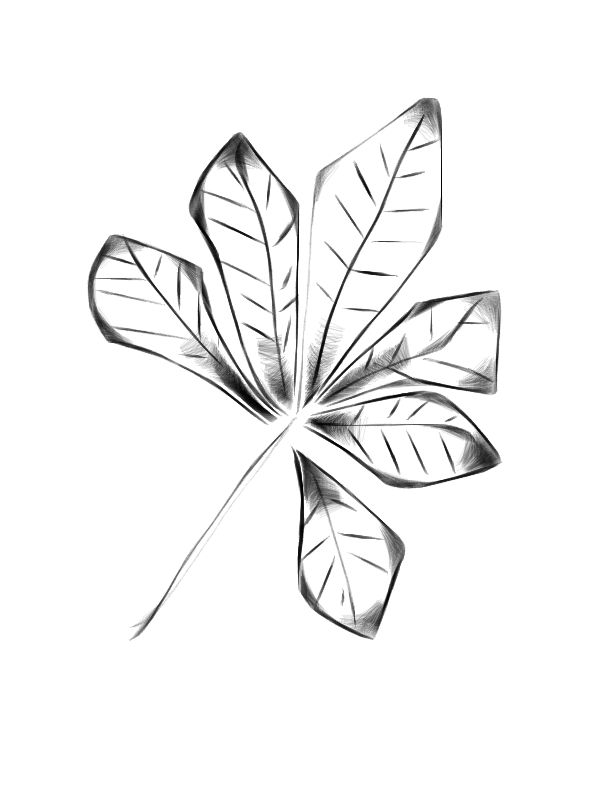
\includegraphics[width=0.50\textwidth]{cover/04.jpg}}

\title{Ересь о Киеве \\ \textsmaller[2]{редакция 10.0}}
\author{Петр Семилетов}
\date{12/03/2022}



\newcommand*{\plogo}{\fbox{$\mathcal{PL}$}} % Generic publisher logo

%----------------------------------------------------------------------------------------
%	TITLE PAGE
%----------------------------------------------------------------------------------------

\newcommand*{\titleAT}{\begingroup % Create the command for including the title page in the document
\newlength{\drop} % Command for generating a specific amount of whitespace
\drop=0.1\textheight % Define the command as 10% of the total text height

\rule{\textwidth}{1pt}\par % Thick horizontal line
\vspace{2pt}\vspace{-\baselineskip} % Whitespace between lines
\rule{\textwidth}{0.4pt}\par % Thin horizontal line

\vspace{\drop} % Whitespace between the top lines and title
\centering
\textcolor{Red}{
{\Huge ЕРЕСЬ О КИЕВЕ}\\[0.5\baselineskip] % Title line 1
%{\Large}\mbox{}\\[0.75\baselineskip] % Title line 2
%{\Huge четвертая редакция}} % Title line 3
}

\vspace{0.25\drop} 
\rule{0.3\textwidth}{0.4pt}\par 

\mbox{ }\\
редакция 10.0\\

\mbox{ }\\
Том 1\\



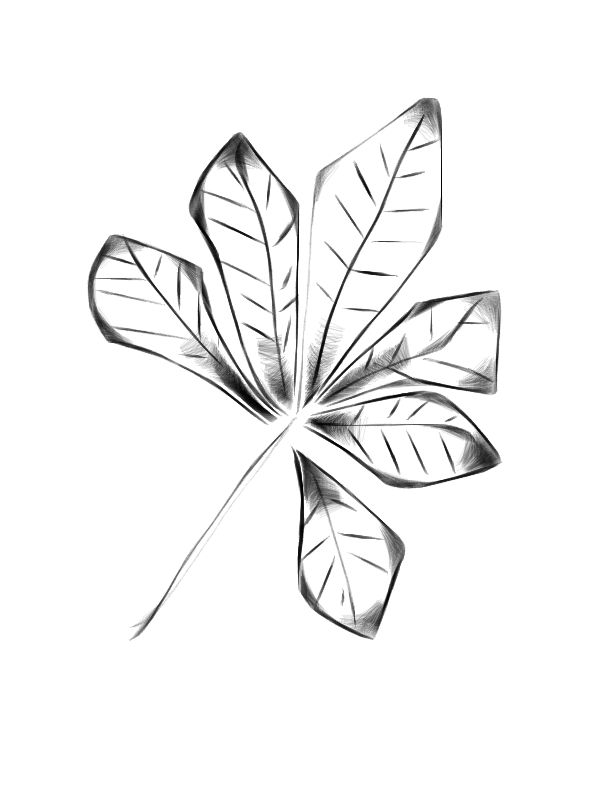
\includegraphics[width=0.40\textwidth]{cover/04.jpg}

\vspace{\drop} 

{\Large \textsc{Петр Семилетов}}\par 


\vfill
%{\large \textcolor{Red}{\plogo}}\\[0.5\baselineskip] % Publisher logo
{\large \textsc{Самиздат 2023}}\par % Publisher

\vspace*{\drop} 

\rule{\textwidth}{0.4pt}\par
\vspace{2pt}\vspace{-\baselineskip} 

\rule{\textwidth}{1pt}\par 

\endgroup}


\begin{document}

\pagestyle{empty}

\titleAT

\newpage

\pagestyle{plain}

\tableofcontents

\chapter*{Предисловие}
\markboth{\MakeUppercase{Предисловие}}{}
\addcontentsline{toc}{chapter}{Предисловие}

\section*{Се начнем повесть сию} 

Никогда не думал, что напишу такую здоровенную книгу. Потуги были. В юности я был ударенный в изучение фольклора, и раздобыл такую амбарную книгу – листы в мелкую клетку, броневая зеленая обложка, вес несколько килограммов. Начал писать в ней энциклопедию славянской демонологии, да застрял. Хотя прежде того сил хватило на четыре рукописных тома народного календаря – «Месяцеслова» – сведенного из множества источников. Приметы, поверья на каждый день.

Так вот сам по себе человек только прозу пишет, а в краеведческих книгах всегда прямо или косвенно участвуют другие люди.

Посему благодарю тех, кто так или иначе способствовали появлению и развитию книги.

Особое спасибо родителям, с которыми обсуждал свои изыскания сразу, как только оные возникали. Коле Арестову за долголетнее краеведческое сотрудничество. Сколько хожено троп, сколько преодолено склонов! Насте, часами выслушивавшей мои исторические выкладки – за некоторые фотки и ценные сведения. Свете Семеновой, Марине Чуприне – за нужные в работе книжки. Неле Арестовой, Андрею Савченко, Саше Ураловой и снова Свете за тонкости перевода с языков, в которых я не силен. Однако не всегда я прислушивался к вашим советам. Алине – за решимость лезть со мной через бурелом всё дальше. Любе – за книжки и сведения о подземле. Зое Колзуновой за некоторые сведения про кости и черепа. Даше Кононюк за совместные краеведческие вылазки.

%Всем кого я не упомянул, дабы ересью не бросать на них тень!
Также и тем, чьими работами я пользовался как источниками.

\section*{С чего вдруг}

Долгое время я не считал себя краеведом, но кажется постепенно стал им. Как увлекся?

С 2005 года мы с друзьями, объединившись под названием «студия Дрымба», снимали любительское кино – вначале на купленную в ломбарде VHS-камеру, затем на MiniDV. В 2009-м стали делать полнометражную фантастическую картину «Сваха», и по ходу запечатлели на видео много краеведческого материала. Брали интервью у местных жителей подле озера Глинка, делали кадры по течению реки Лыбеди, включая тот короткий отрезок, где воды ея бурно протекают в естественном русле под Лысой горой.

«Сваха» зависла, а накопившийся по Киеву материал сподвиг нас к созданию, частью на его основе, большого документального фильма «Киевская сюита», выложенного в сеть в 2010 году сразу после монтажа. Когда мы снимали «Сюиту», пришлось копнуть историю да краеведение на уровне несколько более глубоком, чем листание справочника. Статьи из справочников, как правило – нечто вроде слюны, которую глотаешь, когда очень хочется пить, а никакой газировки под рукой нету и купить негде. Вроде и жидкость, но жажду знания не удовлетворяет.

Спустя год после «Сюиты», весной 2011-го, меня осенило вдохновение писать краеведческую книгу. Я еще не погрузился в предмет целиком, не нырнул в него с головой, а так – опустил туда лицо и пытался открыть в мутной воде глаза. Задумал осветить спорные и загадочные сведения о городе, отчасти поэтому и название выбрал – «Ересь о Киеве», впрочем созвучное другой моей книге, про звукорежиссуру – «Ересь звукозаписи».

«Ересь о Киеве» сначала была сделана как сайт. Это позволяло мне всё время быстро вносить в книгу правки. Читатели спрашивали меня, а нельзя ли выложить её одним файлом? Я неизменно отвечал – нет, ибо мне больше подходит HTML, так удобнее верстать.

Я пользовался множеством книг, большей частью дореволюционных, и прежде выкладывал их в отдельном разделе книги-сайта. То же касалось карт. В конце 2012 года я запустил проект \href{http://semiletov.org/kievograd}{Киевоград}, куда перенес накопленную библиотеку, карты, и также завел там фотоархив и рубрику для фильмов про Киев. Задача Киевограда – предоставление краеведческих материалов по Киеву в свободном доступе.

Медленно пришел я к мысли, что надо таки сверстать электронную книгу, ибо сайт, как ни крути, штука временная. А книгу можно куда-то зафитюлить в сеть, и пойдет гулять. Поэтому в третьей редакции, «Ересь о Киеве» превратилась из книги-сайта в полноценную книгу формата PDF.

Третья редакция стала совершенно новым произведением, от старого сохранившим только название. Это не дополненный вариант прежней книги, превзошедший ее объемом в десятки раз, а именно другое содержимое, выражение иных взглядов.

Началось всё снова с кино. Весной 2013 года мы принялись снимать цикл краеведческих фильмов «Киевская амплитуда». Осенью, параллельно, я стал делать еще один цикл – «Планету Киев». Оба смотрите на Киевограде либо онлайн в Ютубе. 

Съемки расширили мой круг интересов. Я побывал в Змиевой пещере. С Колей Арестовым мы облазили все окрестные склоны. Кирилловские высоты, Логово Змиево захватили меня и привели к открытиям, ставшими стержнем новой «Ереси». Кирилловской пещере посвящаю в книге отдельную часть. Что до видео из пещеры – смотрите «Киевскую амплитуду».

Тогда, в 2013-м, я собирался завершить книгу одновременно с монтажом серии «Логово Змиево», но вот фильм уже был готов, выложен в сеть, а «Ересь» всё писалась, писалась, раскручиваясь по спирали и пуская ветки во все стороны.

Местами она получилась очень подробной, но хотелось поделиться не просто итогом размышлений, но самими размышлениями с исходными данными, источниками. Поэтому, если я в чем-то ошибаюсь, у вас есть всё для проверки или построения каких-то своих выводов.

А работа над четвертой редакцией началась сразу после выпуска третьей, осенью 2015-го. Поначалу это было исправление ошибок (отдельное спасибо за указания на них Александру Петруку) и попутно шероховатостей слога. Вообще я хотел отдохнуть от «Ереси» и стал писать совсем другую краеведческую книгу, легче, меньше.

Но вышло иначе – и появилась новая редакция, еще больше предыдущей, да еще основательно переписанная. Я даже хотел переименовать ее, но кажется, от единожды принятого названия не уйти. 

Хотя по моим ощущениям, получилась совсем другая книга, лишь сохраняющая подобие прежней. Или – книга, более ставшая собой, чем была.

Сразу по выходу четвертой редакции к «Ереси» стал притягиваться новый материал, и дополненная им книга выходит уже в этой, пятой редакции осенью 2017 года. Существенно увеличились и были переделаны главы про Зверинец, Иорданскую церковь и Лысые горы. Точечных изменений претерпели и некоторые другие главы, я уж и забыл какие.

По февраль 2018 года я время от времени вносил в книгу кое-какие изменения и сразу заливал обновленную версию в сеть, но под номером прежней версии.

В конце февраля, добавив еще разные уточнения, мне приходится как бы утвердить их уже шестой редакцией. Отличия от пятой – в точности сообщаемых сведений. 

В седьмой версии были убраны полдесятка фотографий. Иллюстративный ряд теряет в освещении местности, зато книга приобретает первозданную «лицензионную» чистоту. Зарекался использовать чужие снимки, не попавшие в общественное достояние.

К лету 2018 года седьмая редакция обновилась новыми сведениями о болоте Ковпыте и ручье Омелютинке, однако нового в книге не так много, чтобы увеличивать номер основной редакции, посему явилась версия 7.1.

В декабре 2018 года была существенно подправлена глава о летосчислении, что дало повод к выпуску редакции 7.1. В 2019 году была продолжена работа по исправлению, уточнению и дополнению текста. В 2020 оная работа продолжилась, к тому же надо было лучше синхронизировать книгу с другим моим трудом, «Словарем киеведа». 

Так рождалась редакция 8.0, которая дополнилась затем новыми материалами по Зверинецким пещерам и вообще Зверинцу. В восьмой редакции много чего я исправил, проверил приведенные координаты, а также привел их к одному только формату – градусы и минуты, причем не в «правильном» типографском виде, а с обычными двойными и одинарными кавычками, чтобы обеспечить совместимость не только с геодезическими программами, но и популярными электронными картами. 

Девятая редакция книги возникла опять же в ходе согласования с материалами "Словаря киеведа", однако простое согласование обернулось основательным пересмотром некоторых вещей и сверкой летописей по светописным копиям, если они были доступны. Например, я, кажется, таки вычислил место урочища Курган в Бабьем яру. Добавились впечатления от новых краеведческих вылазок. Мне окончательно стало понятно, что пещеру из дела Бейлиса в наше время найти уже невозможно.

Перечитывая старые главы, с горечью убедился, что описанное в них всё более приобретает историческое значение, более не существуя в природе.

Работа над десятой редакцией закрутилась опять же в связи с большой правкой Словаря, а в 2022 году затянулась на, казалось, неопределенное время, пока весной 2023 я неожиданно не вырулил к свету в конце тоннеля. В десятую редакцию добавились две новые большие главы – про Копырев конец и капище Волоса, а поднятые темы затронули, так или иначе, некоторые другие части книги. Вообще про язычество много чего добавилось. Конечно же весь текст так или иначе подвергнулся правке – иногда это касалось буквально поправке на мое текущее мировоззрение, иногда относилось к неточностям в цитировании летописей, краеведческие сведения также уточнялись сообразно развитию моих представлений.

Десятая редакция также ознаменовалась долгими, огромными трудами по упорядочиванию исходника книги. За более чем десятилетие структура книги на жестком диске, в виде файлов и каталогов, развивалась естественным неряшливым образом, например все иллюстрации к такой-то части могли лежать в одном каталоге, а не чтобы на каждую главу по каталогу, куда и текст главы, и картинки. Накопилось множество неиспользованных иллюстраций, их вариантов, и копий в большем разрешении – изначально была мысль выпускать две версии Ереси, с качественными картинками и обычными. Но Ересь до того распухла, что я давно не думал о втором варианте. Весь этот отработанный материал надо было вычленить из исходника, и заново упорядочить структуру, на что и ушло между прочим много месяцев. Если бы не мой редактор TEA и некоторые функции рабочей среды Plasma, то наверное потратил бы и год, а то и несколько.

Одиннадцатая редакция должна была включать в себя дополнительную часть, если не главу – новое важное исследование, однако в ходе правки уже наработанного материала я зацепился за часть про Кирилловские высоты и основательно ее переработал, более строго отнесясь к умозаключениям. Так, я ввел во всю книгу два четко определенных топонима, Хоривица (отождествив ее с отрогом Щекавицы со Старообрядческим кладбищем) и Лысая-Юрковица (указав этим названием на современную гору Юрковицу и предваряя ее прежним названием). Отдельно идет урочище Юрковица. Предполагаемая модель развития именований – именование Хоривицы сползло с исконной такой горы в овраг, со временем исказившись в урочище Юрковицу, и позже переползло на соседнюю с оным урочищем Лысую гору на Кирилловских высотах. Хотя именно на Лысой горе располагался (почему так считаю смотрите в части про Высоты) град Киев, крепость, построенная тремя братьями и названная так в честь старшего Кия, у которого однако уже была своя гора, Киевица.

В одиннадцатой редакции были также заменены некоторые иллюстрации на более качественные, переделаны карты, а еще текст подвергся общей правке.

В редакции 11.2 весьма исправлена последняя глава про Зверинец.

\section*{Электронное издание} 

Я выкладываю «Ересь о Киеве» в сеть как общественное достояние (public domain). Это значит, что вы можете использовать книгу как угодно, в рамках приличий. Проще говоря, вот существует допустим классическое произведение, у него есть сочинитель, но произведение принадлежит человечеству. Так и с этой книгой.

Хотя у электронных книг есть минус. Они имеют судьбу чисто информационную, не привязанную к печатному экземпляру.

У меня на полке стоит книжка «Киев. Справочник-пут\-еводи\-тель» 1954 года издания, небольшая такая, в коричневой обложке, а бумага до сих пор белая. На одной из последних, пустых страниц я нашел карандашные записи:

\begin{quotation}
Справочная \textbf{0-0-9}

Оперный театр

\sout{4-71-84}
\end{quotation}

и под углом:

\begin{quotation}
5-51-34

Оперный театр
\end{quotation}

Эта заметки, судя по телефонным номерам, сделаны примерно во время, когда книга увидела свет – пятидесятые. Кто писал эти строки, чья рука, какая судьба у этого человека? 

Ведь на одной странице развернулась целая история. Сначала человек узнал номер справочной – вероятно, телефон был внове, появился в семье впервые. Затем человек получил один номер Оперного театра. И записал его спокойно, ровно. Позже (насколько?) он получил взамен неправильного номера (который поэтому был перечеркнут) новый, и записал его в спешке, в неудобном положении, наискось!

Книга побывала и в некой библиотеке, чей штамп наполовину стерся, либо был плохо проставлен. А как потом книга попала на букинистическую раскладку – в коробку на асфальте, где среди водорослей можно найти перлы, и всё по одной цене?

В том же чудесном месте – любимом читающими киевлянами и не только ими книжном рынке Петровке – я приобрел еще пару замечательных книг со следами чужих судеб.

Первая – неказистый на вид томик очерка «Киев» Шулькевича. Приехал я домой, рассматриваю – ба, да  этой книжкой владел археолог Дмитрий Яковлевич Телегин. Вот он написал год покупки – «1963». Карандашные пометки на полях, черновой набросок схемы давнего Киева, подчеркнутые строки. И я понял – раз книга Телегина попала на Петровку, сам археолог умер.


\section*{Источники} 

Конечно же, источники, приведенные мною в конце книги – лишь малая доля общего их объема, туда я поместил лишь цитируемое. Выдержки, если они на старославянском либо «роськой мове» Великого княжества Литовского, даю в подлиннике. Важнейшие цитаты на латыни или греческом стараюсь приводить в своем, по возможности точном переводе, а также в подлиннике. При цитировании летописей, для удобочитаемости помещаю из обработанных учеными текстов Полного Собрания Русских Летописей, где подлинник трактован и потому несколько искажен. Наиболее важные выдержки, однако, беру из светописных копий подлинников.

\section*{Об иллюстрациях} 

В качестве иллюстраций я использую много старинных фотографий и изображений, за давностью лет перешедших в общественное достояние. Существует много фоток, которые я хотел бы показать в этой книге, да не могу из-за авторского права и всяческих связанных с ним ограничений.

Современные снимки в этой книге сделаны, за редкими исключениями, мною и отдаются в общественное достояние.

Увы – изображения, полученные со спутниковых карт, сурово защищены всевозможными коммерческими лицензиями, поэтому я вынужден был, несмотря на всю заманчивость, отказаться от них, за редкими исключениями и с указанием копирайта. Из лицензионных соображений я использую лишь старые карты, которым больше 70 лет – они перешли в общественное достояние. Иногда я помещаю советские карты, да немецкие аэрофотоснимки 1918 и 1943 годов.

\section*{О координатах}

Поелику книгу я пишу для вечности, а городские адреса бренны да изменчивы, буду частенько давать координаты, в геодезической системе WGS-84, которая сейчас используется в GPS и большинстве электронных карт. В СССР была другая система координат, СК-42. Есть еще СК-63. Существуют формулы пересчета из одной системы в другую, программы, онлайн-конвертеры, различные макросы и тому подобное. 

Я привожу координаты в формате градусов и минут. Пример: "50°28'6.66"N 30°29'56.42"E". Буква N означает «North», или северная широта. E – «East», восточная долгота.

В старых редакциях книги я давал еще координаты в десятичных градусах. Пример: 50.468517°, 30.499005° либо без знака градуса. Сначала идет широта, потом долгота. 

\section*{Программное обеспечение} 

В работе над этой книгой мне помогало разнообразное программное обеспечение, о чем я не могу умолчать.

Вся работа уютно происходила под операционной системой Linux, в дистрибутиве Mageia и рабочей среде KDE, а с лета 2017 года – в среде Mate. С 2019 года работаю уже в Manjaro Linux, а в 2020 перебрался в Arch, а затем сменил Mate на KDE/Plasma. 

Текст я набираю и верстаю в редакторе \href{http://semiletov.org/tea}{TEA}, собственной разработки. Программа Okular всегда под рукой для чтения сканов в форматах PDF и DjView. Вёрстка подготовлена при помощи удивительного средства вёрстки \href{http://www.latex-project.org/}{\LaTeX} с движком Lua\TeX~ – с ними я могу одновременно сочинять книгу и верстать её, не разделяя текст и макет. Я использовал семейство свободных шрифтов DejaVu. Иллюстрации подготовлены в растровом редакторе GIMP и векторном Inkscape.

%Оно не только выглядит так, как мне нравится, но и позволило, наряду с поддержкой кодировки UTF-8 в Lua\TeX, сочетать на страницах текст на кириллице, греческом и других языках. 

%При этом я подключил следующие пакеты функций – не могу умолчать оные, ведь от них зависит многое, что повлияло на вид книги: protrusion, polyglossia, verse, graphicx, pdfpagelabels, bookmark, relsize, tocloft, calc, multicol, longtable.


\section*{Ересь в Сети. Пишите письма}

Новые редакции книги, по мере их выхода, будут выкладываться по следующим адресам:\\ 

\noindent
\href{http://semiletov.org/kiev}{http://semiletov.org/kiev} (мой сайт)\\
\href{https://www.facebook.com/groups/213781655750601/}{www.facebook.com/groups/213781655750601} (группа Киевоград в ФБ)\\
\href{https://t.me/kievograd}{t.me/kievograd} (группа Киевоград в Телеге)\\

Также можете написать мне письмо по электронной почте: \href{peter.semiletov@gmail.com}{peter.semiletov@gmail.com}, 
в телегу: @petersemiletov или ФБ/Мессенджер \href{https://www.facebook.com/peter.semiletov}{www.facebook.com/peter.semiletov}. Буду рад отзывам, указаниям на ошибки, дополнениям.


\part{Колебание основ}

\chapter{Начало}

Как возник Киев? Долгое время меня не заботил этот вопрос. Ведь ученые, следом за Нестором-летописцем, всё давно пояснили. Еще дошкольником в начале восьмидесятых я знал, что город основали Кий, Хорив, Щек и сестра их Лыбедь. Я представлял их себе именно такими, как потом увидел в 1982 году, когда город отмечал 1500-летие – медными  скульптурами на лодье, у свежего Днепра в парке Примакова, что раскинулся вдоль каменной набережной Днепра от моста Патона до Моста метро. 

Благообразные, похожие на первопечатника Ивана Федорова славяне-бородачи – кроме Лыбеди, конечно – с долгими волосами, взятыми в обручи. Двое с копьями, один с луком, и ни у кого нет вёсел. Поначалу это была железобетонная скульптура, обшитая медными листами. С 2010 года материал заменили на бронзу, а лодью уменьшили. К ней любят приезжать фотографироваться молодожены.

Небольшая модель этого памятника в промежутках между похищениями стоит во дворе Художественной академии на Вознесенском спуске (улица Смирнова-Ласточкина). Она же Вознесенский спуск. Улицы переименовывают туда-сюда, не уследишь. Здесь и далее придерживаюсь привычных мне названий. 

Там же в усадьбе академии, многие здания разукрашены замечательными граффити – надо лишь завернуть за само здание с правой его стороны, к склону холма, и пройти вдоль главного корпуса. А еще можно найти на задворках мусорник со скульптурами. Но про ту, весьма историческую местность – позже!

Лодья, набережная... Почему пишу здесь и далее «лодья»? Так правильно. Так в летописях. Так говорили – л\'одья. Производное – лодка. Вы же не говорите – ладка. Посему – лодья. Ученые-языковеды возразят, что с буквой «о» это северный говор. Нет, это давнее произношение, позже в некоторых местностях изменившееся на «а». Ученые могут почитать летописи и убедиться, как было прежде.

\begin{center}
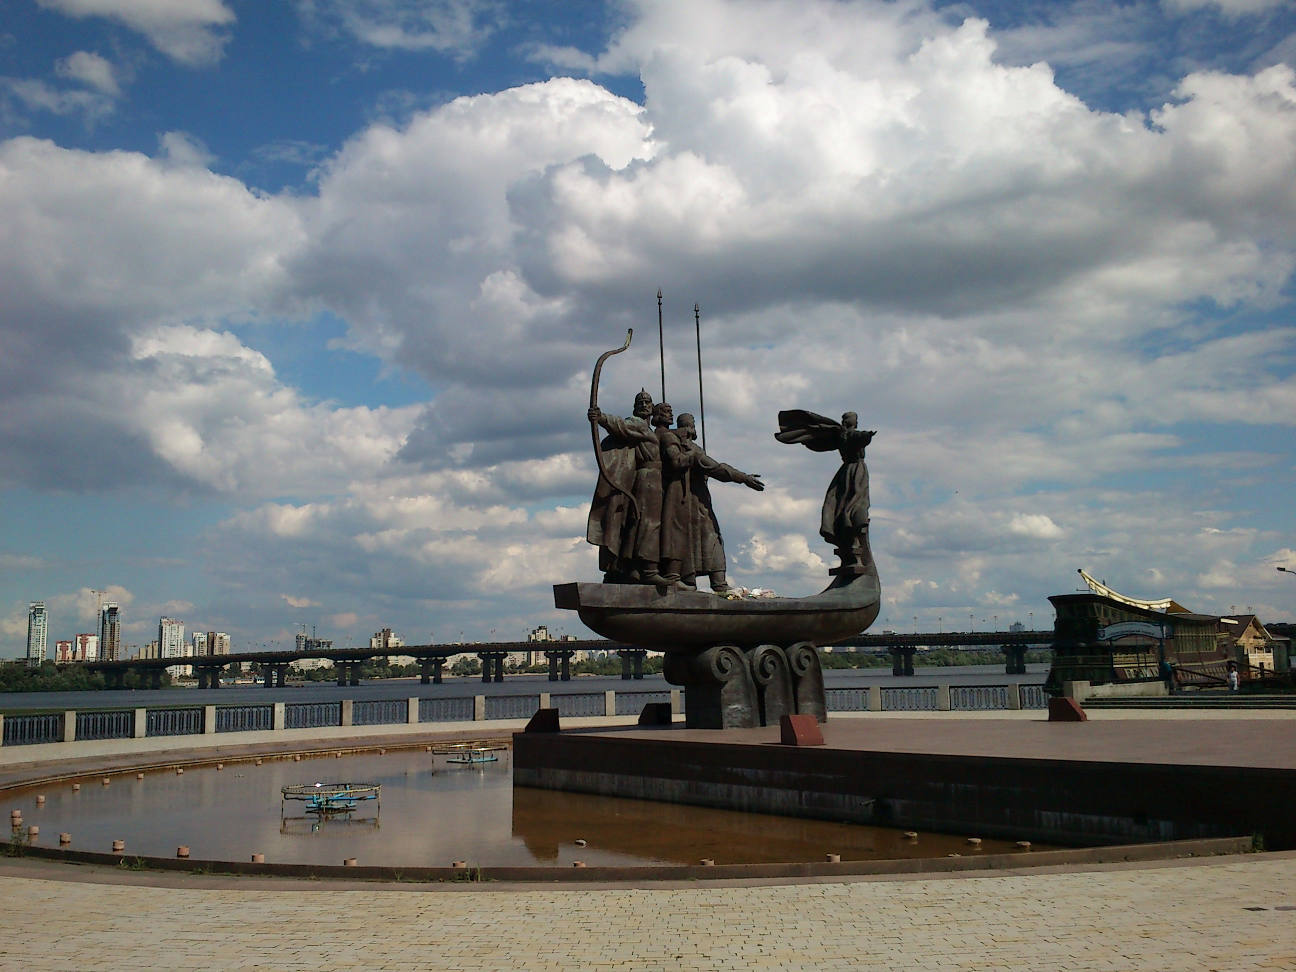
\includegraphics[width=\linewidth]{chast-colebanie-osnov/nachalo/ladiya.jpg}
\end{center}

%Небольшая модель этого памятника в промежутках между похищениями стоит во дворе Художественной академии на улице Смирнова-Ласточкина. Она же Вознесенский спуск. Нынче трудно писать книги – улицы переименовывают туда-сюда, не уследишь. Здесь и далее придерживаюсь старых, привычных мне названий., %ибо не могу переписывать книгу согласно каждому новому решению городского совета!% За исключением, когда новое название нравится мне больше.


%Там же в усадьбе академии, многие хозяйственные постройки разукрашены замечательными граффити – надо лишь завернуть за само здание с правой его стороны, к склону холма, и пройти вдоль корпуса. Пишу по памяти, может уже закрасили.

Я смутно помню время, когда лодьи со скульптурами и каменной набережной не существовало. До конца восьмидесятых, в парке Примакова был песчаный пляж, у пляжа пристань-понтон, и плавал катер на противоположный берег – южную часть острова Гидропарка, тоже с пляжем.

А под горой напротив парка Примакова разворачивался у моста Патона трамвай, что ходил вдоль древних, изрытых пещерами и сочащихся рыжими родниками холмов с Лаврой и Аскольдовой могилой, по набережной до Красной, ныне Контр\'актовой, площади. Этот чудесный маршрут упразднили. Печатно обещали – временно, оказалось – навсегда. Рельсы продержались, ржавея, дольше трамвая. На моей памяти он был одновагонный, красный.

\begin{center}
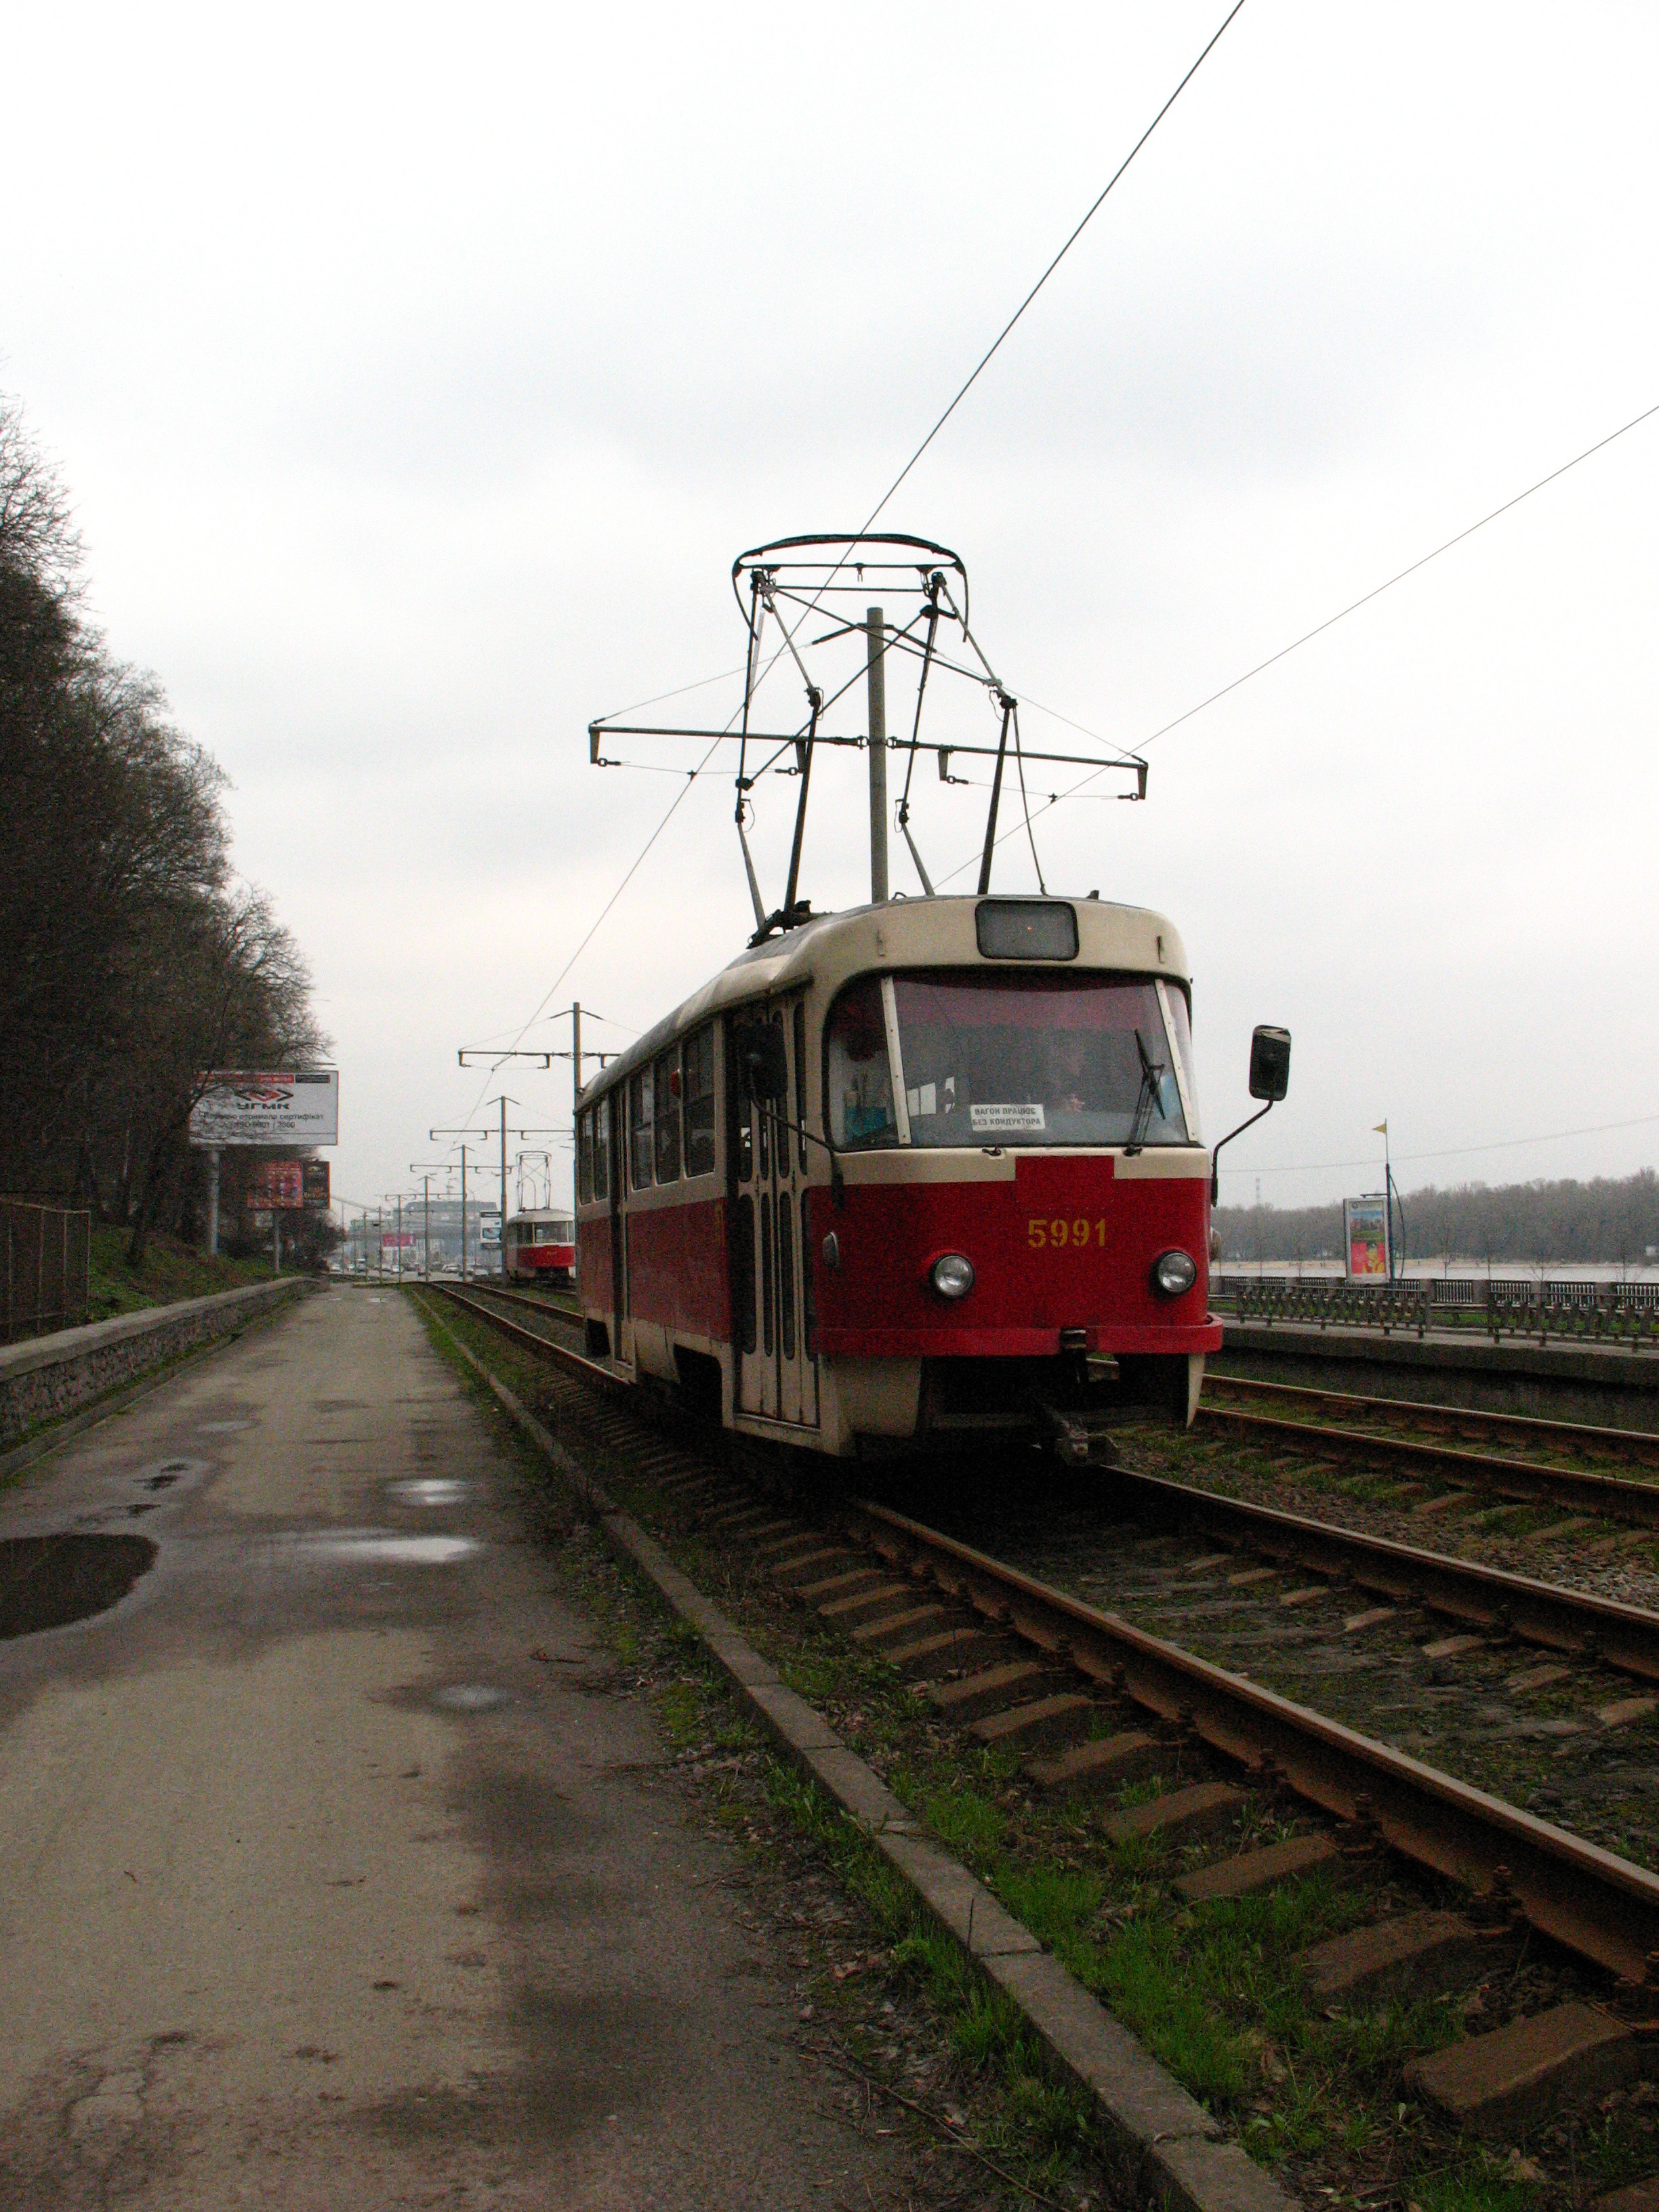
\includegraphics[width=0.70\linewidth]{chast-colebanie-osnov/nachalo/tramvay-no-5.jpg}

\textit{2008 год, на пятом маршруте трамвай «Татра» модели T3 или T4SU.} 
\end{center}

Кто не в курсе – трамвай ходил и по мосту Патона. Маршрут номер 27\index{Трамвай №27} длился от бульвара Перова до Дворца спорта, это 17,4 километра, что проезжалось чуть больше чем за час. А 35-й\index{Трамвай №35} маршрут начинался на Березняках, был разворот там где сейчас высотки возле Русановского канала, ближе к железной дороге – и заканчивался у Центрального вокзала на правом берегу. Под горой со статуей Родины-матери, около моста Патона, был большой пересадочный узел. Одна ветка шла по набережной Днепра, другая по мосту, и дальше тянулась мимо холма с музеем ВОВ и по улице Старонаводницкой, Клову и дальше в центр.

Сидишь себе да глядишь в окошко, а колеса гремят по рельсам. Печка греется. В тех старых трамваях хорошо думалось. Нынче не то, и огурцы уже не те, и пупырышки на них фуфло против давнишних.

%Но что делает капитализм с удобными и длинными маршрутами трамвая? Он их отменяет и разбивает путь на мелкие отрезки, чтобы вы делали больше пересадок. Готовь деньги! Кроме того, упраздняется сам трамвай и людям предлагается ездить в маршрутных такси. В свою очередь длинные маршруты и этих передвижных иконостасов отменяют в пользу коротких – теперь уже коммунального транспорта. Та же хитрость на новый лад.


\begin{center}
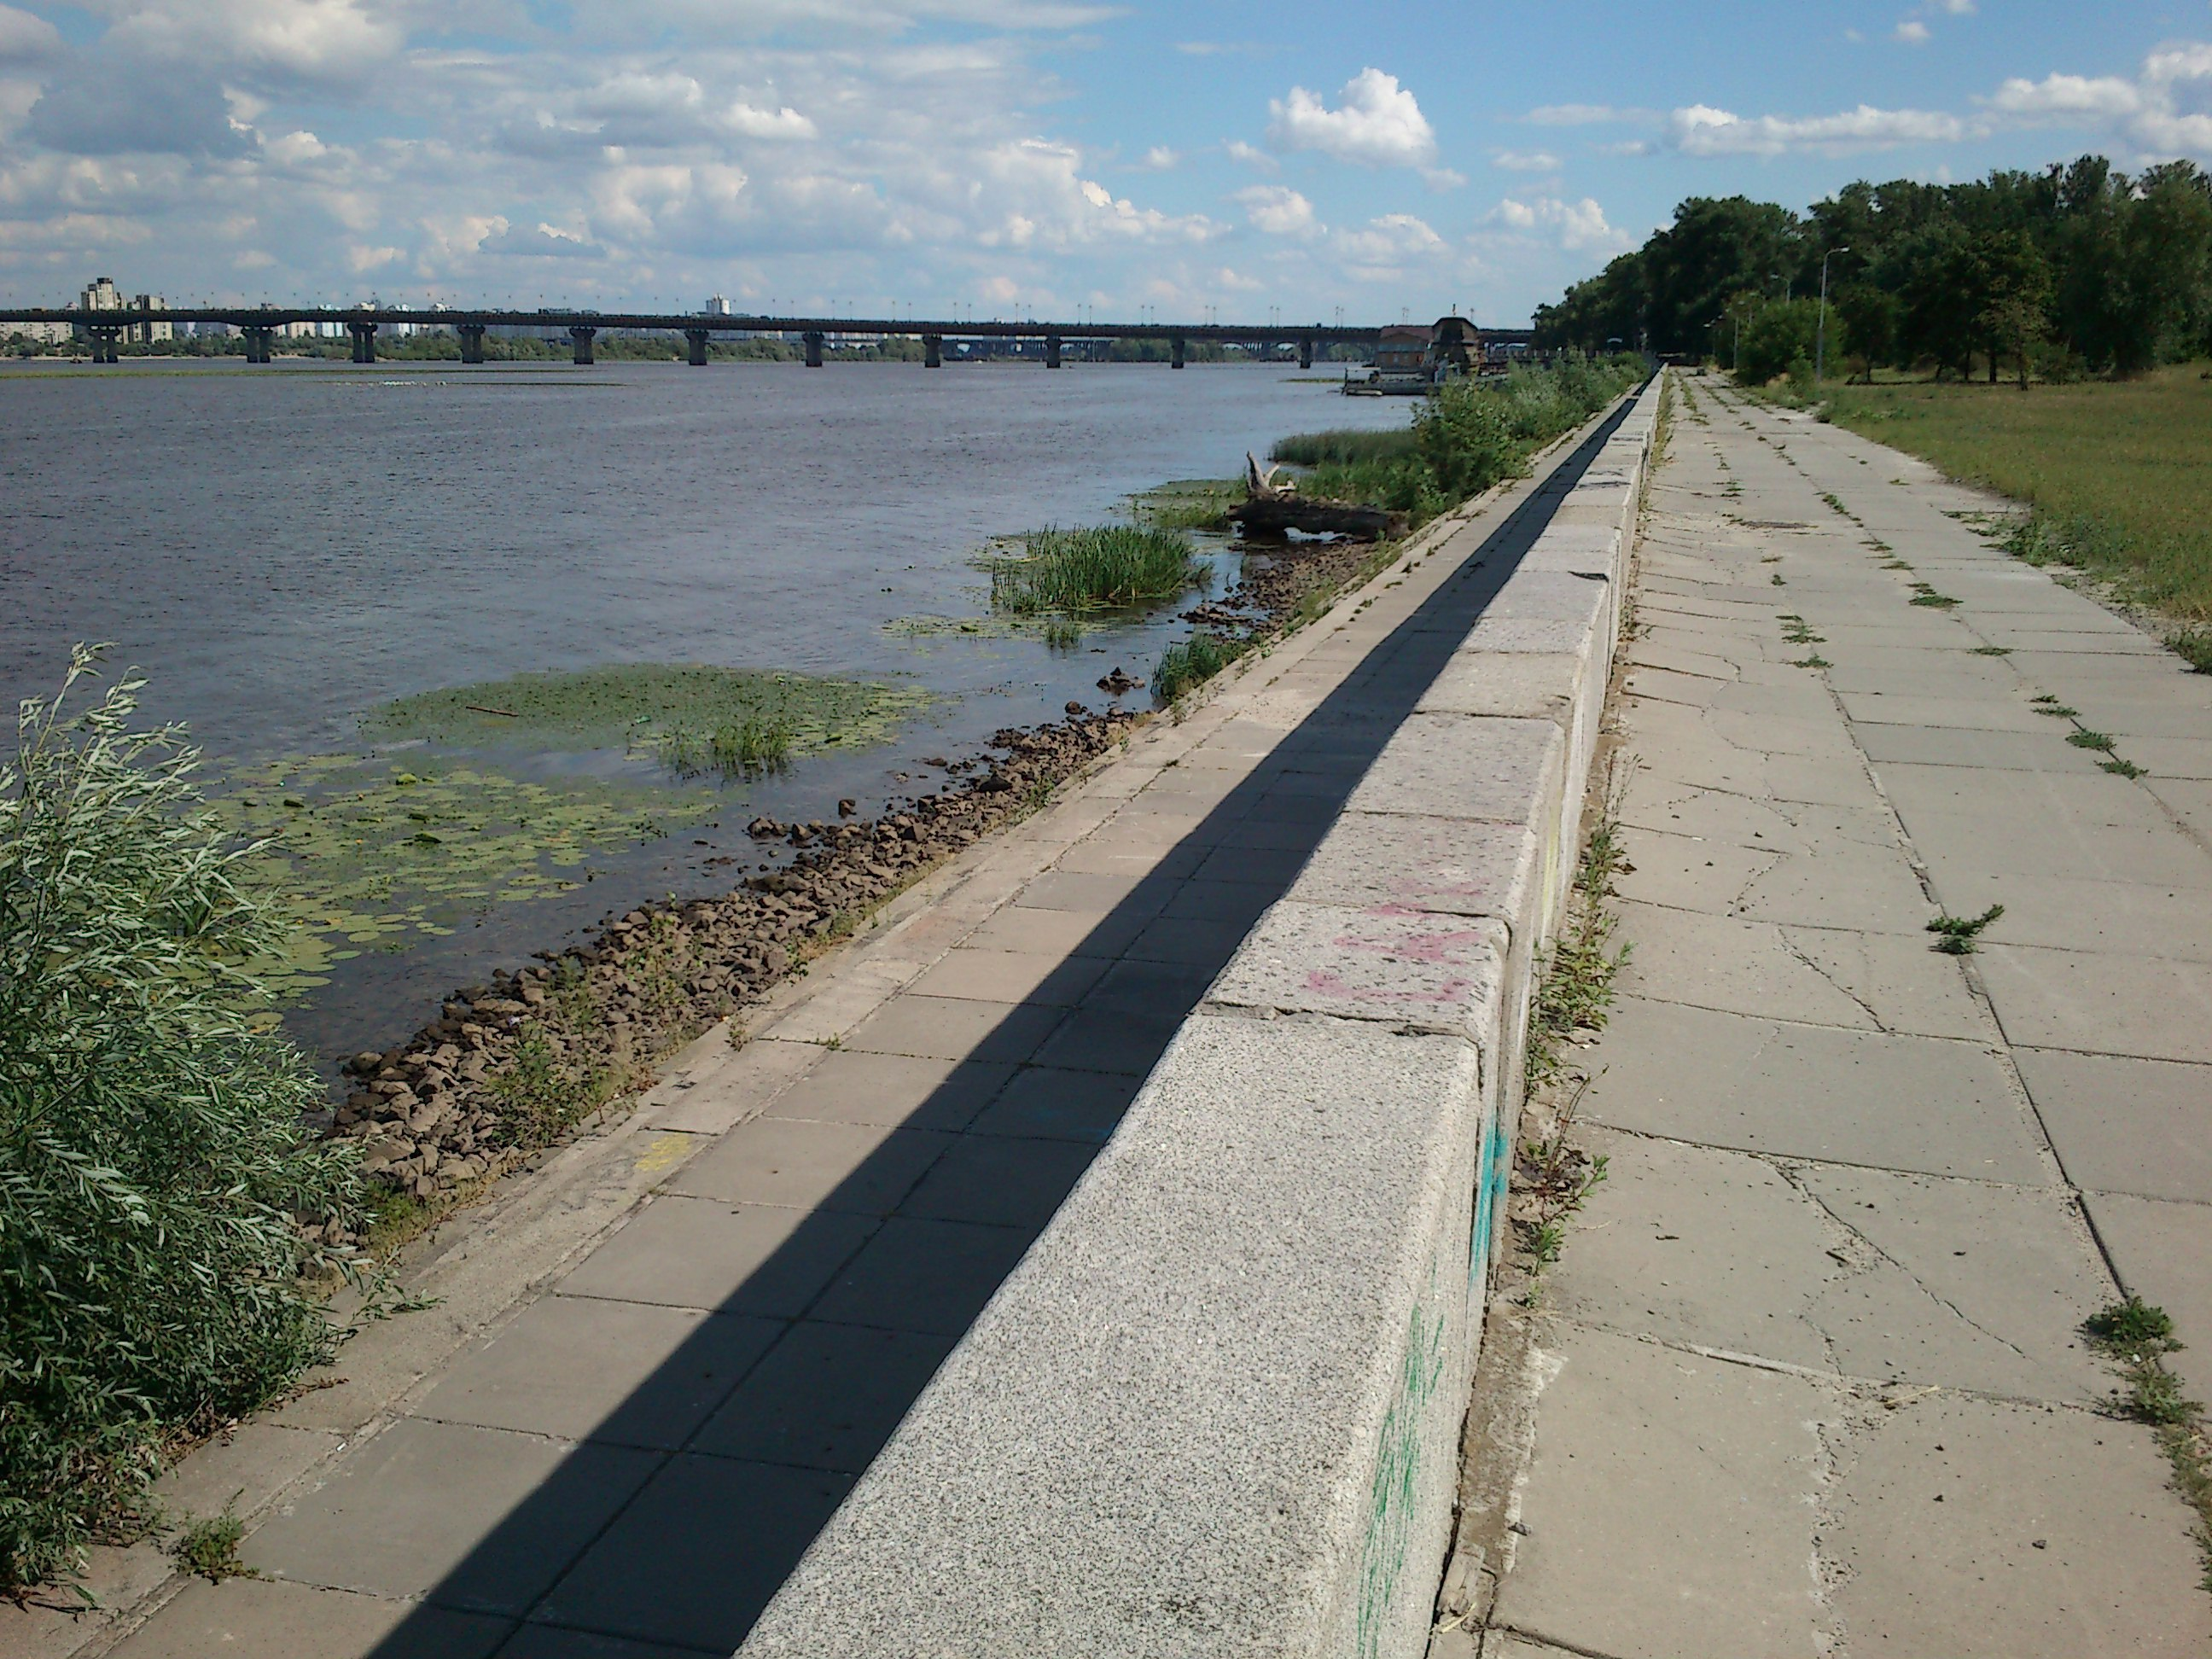
\includegraphics[width=\linewidth]{chast-colebanie-osnov/nachalo/primakova-01.jpg}

\textit{Парк Примакова, лето 2012 года.} 
\end{center}

В первом десятилетии нашего века, парк Примакова переименовали в Наводницкий и отчекрыжили от него кусок под аллею Славы миротворцев ООН. Некогда тихий парк вдоль реки, с высокими тополями и яркими цветочными клумбами, ныне застроен культовыми сооружениями, а у берегов стоят плавучие рестораны. И едут, едут машины по аллеям.

В девяностых я часто гулял там с Бобиком, моей собакой. Мы спускались туда с холмов Зверинца, от Бастионной улицы\index{Бастионная улица}.

Вот так выходишь утром из дому, а во дворе ни души, а тишина, и тепло – потому что весна и май начался. Проходишь через Собачку\index{Собачка} – крутой, продавленный глубокими ярами склон горы, весь поросший одичалыми садами. Вишня в белом цвету. Налево от Собачки, к Бастионному переулку – обрыв с бетонной подпорной стеной, за нею топорщится из ямы белопанельный Дом художников.

Там обитали художники, а их мастерские глядели широкими окнами в самое небо на высотах последних этажей. Кроме прочих жил в доме том странный человек. Он бросал с балкона вещественные плоды раздумий в пакетах из плотной бумаги, перевязанных шпагатом, эдакие бандерольки случайным прохожим.

Так уродство соседствовало с прекрасным – с сосредоточенными творцами, цветущими деревьями, и той сладковатой душистой смолой, которая сочится из узловищ в стволах вишен. Всё время забываю, как эта смола называется, а это вдруг вспомнил – камедь.

На Собачке есть две главные тропинки. Верхняя вдоль забора ботсада (мы его называли «ботаника» или «боташа»), а нижняя примыкает к опорной стене. Еще две сохранившиеся служат для подъема, в начале и конце Собачки. По ним, особенно той, что близ родного двора, я любил кататься на санках.

Нижняя тропа сейчас совсем запущена – ее перегораживает бурелом, а когда-то там свободно гоняли на велике. Посередке тропы был пятачок, широкое место, и оттуда лесенка наверх, к спортплощадке. Лесенка из деревянных, вбитых в землю дощечек. Ее делал художник Михаил Фомич, фамилию не помню. Он жил прямо напротив этого пятачка. На 2024 год и след той лестнички простыл...

Словом, по нижней тропке, кажется, никто больше не ходит, это трудно. Полагаю запустение оттого, что улица Мичурина, к которой, по сути, добирались по нижней тропе жители верховий Бастионной улицы, претерпела смену населения – давний частный сектор застроили теремами новые здесь люди.

А вот верхняя тропа осталась, утоптанная, по ней и к ней ходят в поисках дырок в ботсадовском заборе.

\begin{center}
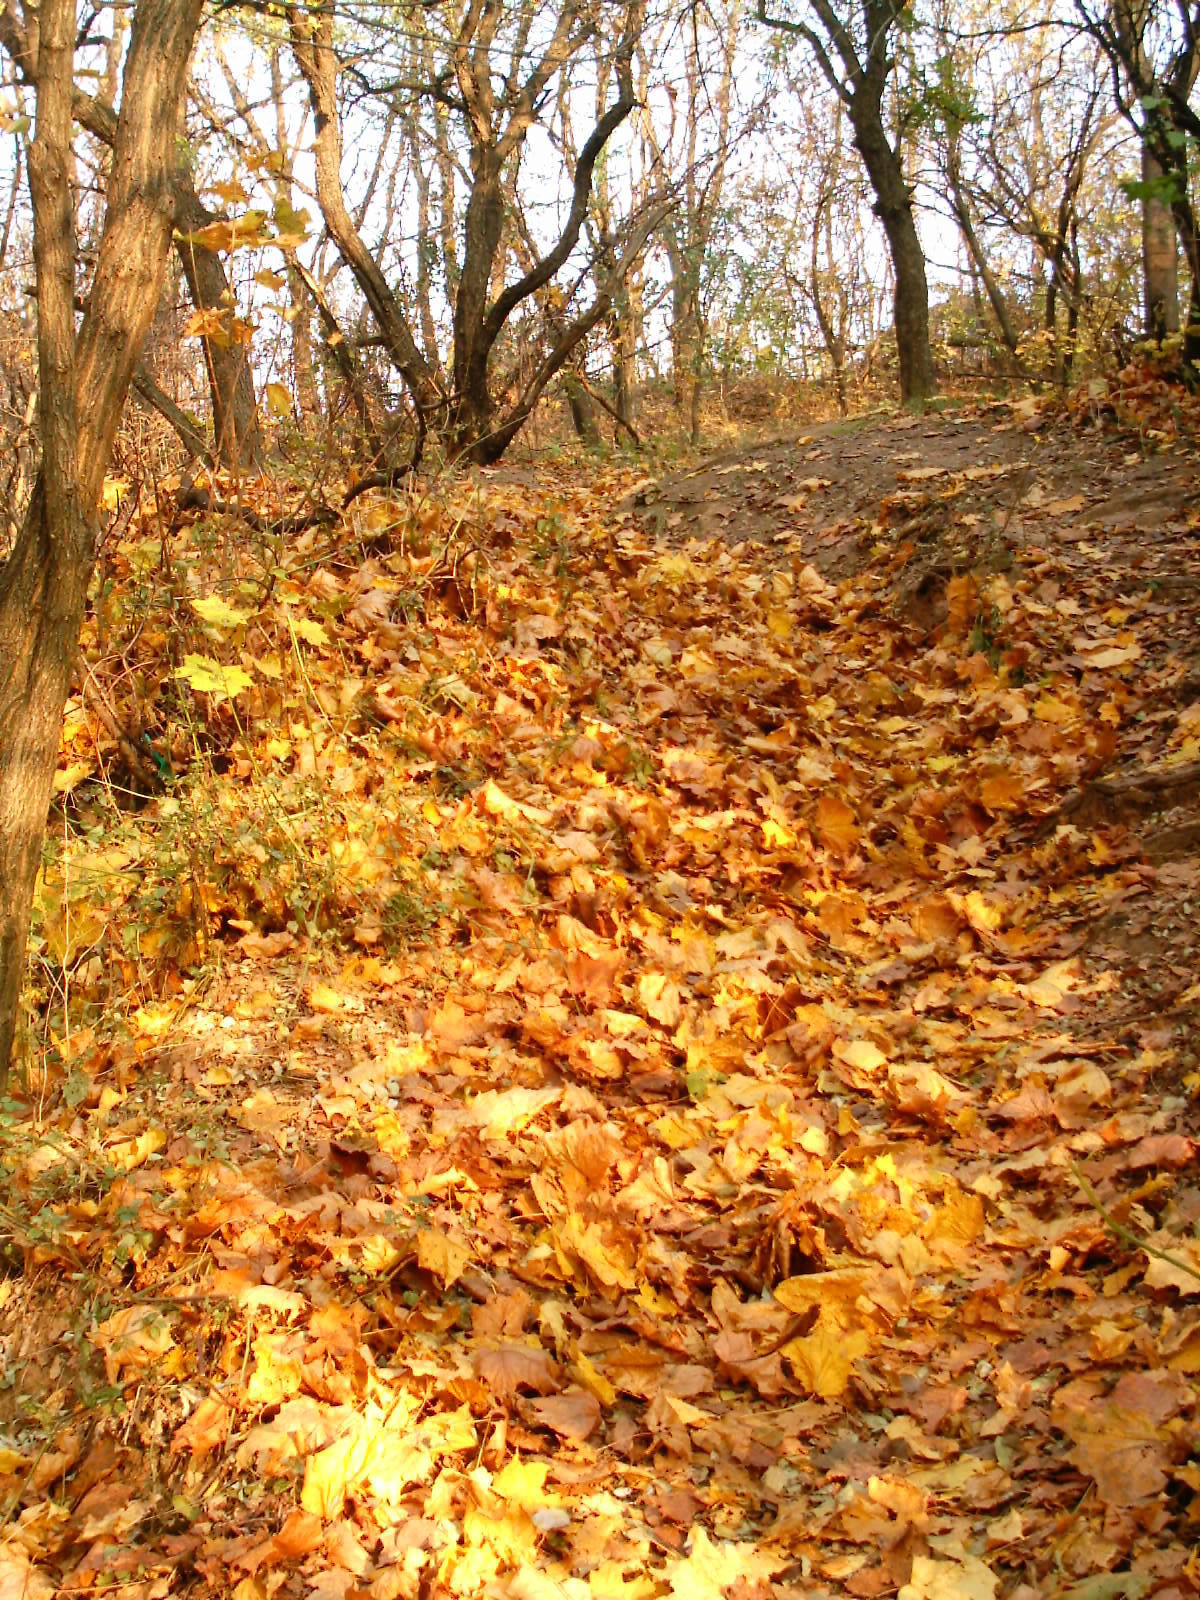
\includegraphics[width=0.85\linewidth]{chast-colebanie-osnov/nachalo/sob-imag0038.jpg}

\textit{Собачка, путь наверх, 26/10/2005.} 
\end{center}

А тогда! Зимой, вечером уже, когда тишина стоит и небо светлое от снежных туч, а фиолетовый снег искрится золотом, летят санки вниз накатанным по тропе желобом, повторяя все изгибы обрыва, и не надо рулить и тормозить, только в конце ежели не успеваешь повернуть левее, продолжая ход в желобе, то выбрасывает тебя в приземистые вишни, почти кусты, и санки в них застревают, а ты проваливаешься через ветки дальше. На верхней, посадочной площадке, у забора ботсада, растут орехи. Потом проезжаешь под грушами. И наконец – вишни!

А вот летом идешь по нижней тропинке, а из кустов высовывается сумасшедший с отверткой-заточкой. И потом исчезает, собаку увидав. А то еще находишь там же здоровенный разводной ключ, который по сей день исправно служит.

На Собачке было ровное место со спортивной площадкой с оградой из сетки. Туда, по террасам среди диких вишень, поднималась лестничка Михаила Фомича, переходившая в грунтовую дорожку. На площадке стояли даже тяжелые металлические футбольные ворота, а на возвышении в рост человека, таилась под сиренью скамейка. Местные играли тут в футбол, выгуливали собак, а на лавке заседали любители поиграть на гитаре.

Еще в конце девяностых, со спортплощадки украли ворота. Сначала одни, потом вторые. Затем, по мере удаления от социализма, исчезали покрывшиеся ржавчиной части ограды, глинистая полянка зарастала травой, ползла вниз зелень с пригорка, уже не сирень, а нечто совсем дикое.

Северная сторона Собачки выходит ко глубокому яру. На противоположном его берегу – остатки погребов. В начале 21 века в них жили беспризорные дети. Затем погреба пришли в совсем удручающее состояние, а яр усеялся мусором. Выше погребов начинается частный сектор на улице Мичурина.

От Собачки мы с Бобиком, пройдя мимо нескольких «гостинок» и сойдя по лестничке у некогда единственной в районе шестнадцатиэтажки, сворачивали на эту улицу. Она тогда была очень мирная, с гнилыми, косой гармошкой, деревянными заборами, за них лезла лапами наружу сирень. В гуще садов прятались домики. Летом на ходу вишню в рот отправил, водную колонку близ обочины покачал, горстью выпил студеной воды – и дальше. Редкий прохожий встретится.

Нынче там – современные терема и бетон, и должен вжиматься пеший человек в новокрепостную стену, чтобы не быть смазанным в месиво не то машиной, не то танком, принявшим облик автомобильный. Раньше название улицы вполне оправдывалось её зеленью – и наверное, были в садах сорта, выведенные самим Мичуриным. А рядом с теремами садов нет. Поставят эти кусты-пудели и наймут садовника, чтоб их подстригал. Барскому глазу приятно смотреть.

\begin{center}
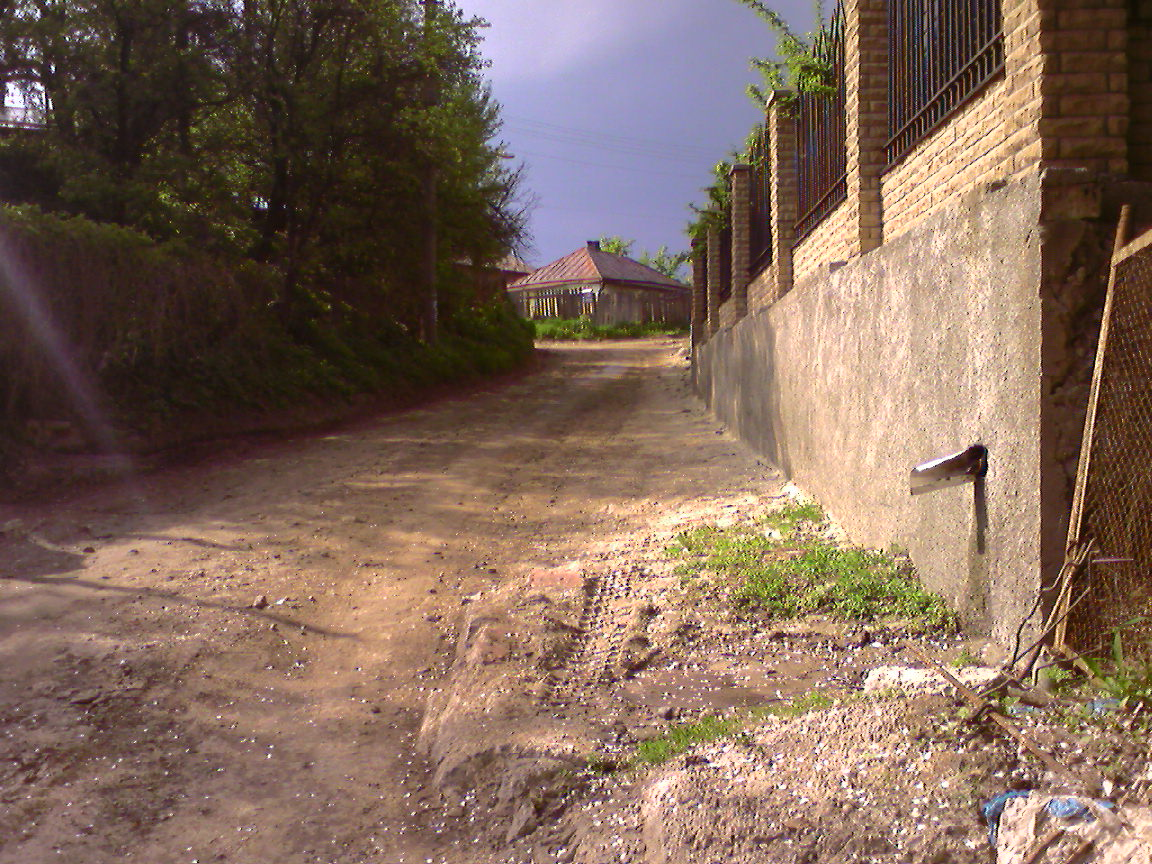
\includegraphics[width=\linewidth]{chast-colebanie-osnov/nachalo/lomakovskaya01.jpg}

\textit{2006 год, улица Мичурина, впереди – перекресток с Пирятинским переулком.} 
\end{center}

Улица Мичурина, бывшая Ломаковская, по крайней мере с 18 века
идет в устроявшихся пределах по всему склону северного Зверинецкого холма, посередке его ската, вбирая в себя узкие улочки и переулки, лестницы и лестнички. Одинокая скамейка ближе к перекрестку с Пирятинской улицей наводила на мысль о каком-то редком автобусике, что мог здесь курсировать в давние времена, как 76-й маршрут\index{Автобус №76} по Зверинецкой, хотя крутизну гор на Мичурина, кажется, не сможет преодолеть ни один автобус.

На моей памяти, не было там и магазина, а лишь частные усадьбы, водяные колонки, просмоленные деревянные столбы, синие почтовые ящики на множество дверок, да две таксофонные будки. Одна, почти в начале Мичурина, около лестнички под шестнадцатиэтажкой, прославилась тем, что в ней укрылась от разозлившегося козла какая-то бабка. Козел всё же проник внутрь и бабка сдерживала его, ухватив за рога. Другая будка стояла подле перекрестка с Пирятинской. 

\begin{center}
\includegraphics[width=\linewidth]{chast-colebanie-osnov/nachalo/\myimgprefix 13092009653.jpg}

\textit{2009 год, улица Пирятинская, впереди – перекресток с Мичурина.} 
\end{center}

Оттуда можно было свернуть на север, в сторону бульвара Дружбы Народов. Спускаешься в тени деревьев по громадной лестнице – теперь так нельзя, улица Пирятинская прерывается посольством, и лестница прикреплена уже к нему. Внизу же, правее, в сырой ложбине холма журчал вкусный родник\footnote{50°25'25.7"N 30°33'46.9"E}, слывший целебным. Возможно, в давние времена он назывался Рожницей. Сюда в восьмидесятых-девяностых издалека приезжали с бидонами люди. И там построили автозаправку. Существа из карбона и металла хотят пить горючее. Иди дальше, зверь из плоти. Купи себе воду в баночке.

Лестницей я возвращался, домой, а в парк Примакова двигался дальше по улице Мичурина, до самого ее конца, где очень крутой спуск. Однажды я съехал с него, полностью заледеневшего, на санках. Здесь застройка новоделами началась раньше всего.

\begin{center}
\includegraphics[width=0.80\linewidth]{chast-colebanie-osnov/nachalo/\myimgprefix IMG_20150601_133144.jpg}

\textit{2015. Спуск на Мичурина. Прежде, слева были сады за деревянными заборами, а справа – поле с подсолнухами.} 
\end{center}

И вечно до половины этого спуска доходили, темня треснутый асфальт и камни, ручьи – то ли родники, выбивающиеся из-под люков, то ли вода, накачанная из колонок.

Вообще этот отрезок улицы Мичурина держится за нею больше на бумаге, ибо там по прямой как бы продолжается улица Землянская. Она же прежде, взобравшись на гору, лежала и по другую сторону забора ботсада, через нынешний участок хвойных растений, отмежевывая его от сирингария. Там поныне есть аллея, но мало кто знает, что это бывшая улица.

Землянская улица вливалась в Выдубицкую, что еще начале сороковых годов двадцатого века пересекала всю местность будущего ботсада примерно от Бастионной улицы и до Выдубицкого монастыря. И перекресток Землянской и Выдубицкой был там, где сейчас перекресток у верха Сиреневой аллеи, с поворотом к хвойным, сирени, Ионовской церкви да назад к выходу из ботсада.

Старые домики на Мичурина держалась долго. Я ходил по улице из года в год – ничего не менялось.

Но вот одна из усадеб обезлюдела. Пустые висели меж яблонь качели. Стала врастать в землю калитка, за несколько лет одичал сад, хотя соседи еще пользовались его плодами. Сам домик вначале сохранял жилой вид, а потом просела над входом крыша, треснули, принялись осыпаться стены – через отвалившуюся штукатуру проглядывала дранка, косая решетка из досочек. 

Этот единственный на улице выбывший из строя дом оказался предвестником грядущей волны таких угасаний с последующим пришествием новых хозяев. А те выкорчевывали сады, срывали части склона для умещения огромных фундаментов строящихся жилищ.

Не люблю больше бывать на Мичурина. Пусть остается в моей памяти какой была. До соединения с Землянской, улица поворачивала и круто спускалась, там еще на пригорке справа стоял деревянный дом – номер сорок? Всё это срыто, даже сама улица теперь смещена.

Землянская и одноименный переулок напоминают о местности Землянке, прозванной так по близости к Зверинецким пещерам, либо от земляных укреплений Зверинецкой же крепости, что некогда покрывала многоугольником валов половину нынешнего ботсада и сгинула окончательно при его строительстве в 1940-х.

Пещеры на моей памяти сначала были закрыты для посещений. Не стояли рядом две церкви, всё выглядело иначе. Вход располагался в обычной частной усадьбе на Мичурина. В шестидесятые к нему приладили будку туалета, которую потом передвинули по просьбе археологов. А в конце девяностых в пещеры начали водить паломников, сверху горы, через проем в стальном, из ребристых прутьев, заборе ботсада.

Там рядом с плантацией кормовых культур был плоский участок, куда свозили торф – как понимаю, место дореволюционной церкви над пещерами – и вот за торфом пропилили в ограде большую дырку, может даже с калиткой, не помню. Потом уже подключился близлежащий Ионинский Святотроицкий монастырь и в нулевых на месте нескольких частных усадеб возвели Архангело-Михайловский Зверинецкий монастырь. Сами же пещеры утратили свой исконный вид еще в начале 20 века, будучи приспособленными для паломников. Сейчас это еще более облагороженное подземелье.

Назову основополагающие работы про эти пещеры, тоже начала 20 века.

Полная чудес брошюра иеромонаха Серапиона «Новооткрывающиеся древние пещеры в Киеве, на Зверинце», вышедшая в Киеве в 1914 году. 

Банковский служащий и одновременно опытный археолог Александр Дмитриевич Эртель\footnote{Много изучал киевские курганы, пещеры, валы и городища, в том числе пещеры в Китаево, курганы в Совках, могильник около Проневщины. К слову, брат Эртеля, Леонид, с 1914 года проживал на Ломаковской (или по Ломаковскому переулку), 37-А.}, крайне правый монархист, написал в 1913 году брошюру «Древние пещеры на Зверинце в Киеве».

Киевский историк Иван Каманин\footnote{Каманин оглох после болезни, что повлияло на выбор рода деятельности – работу в Киевском центральном архиве древних актов. Много печатался в дореволюционных околоисторических изданиях под своей фамилией и псевдонимом А. Щуровский. Каманина, согласно завещанию, в 1921 году похоронили в тех же Зверинецких пещерах – одна из стен его склепа, кирпичная, граничит с концом «Алтарной улицы».} год спустя выпустил более объемный труд «Зверинецкие пещеры в Киеве»\cite{kamanin01}.

И в 1918 году профессор Киевской Духовной Академии Николай Петров подытожил работы Эртеля и Каманина, добавив кое-какие источники, книжечкой «Ученые труды по исследованию ново-открытых в Киеве Зверинецких пещер».

%Везде, где рассуждений больше, чем описания, возможно искажение сути, возникающее в мыслях сочинителя. Логические ошибки, невнимательность, наконец личное мнение, окрашивающее любые рассуждения и зачастую отсекающее ряд доводов – всё это вносит путаницу, а путаница, в отличие от кругов по воде от камешка, не угасает, но увеличивается – чем дальше от источника, тем она сильнее. Но хуже всего, когда пытаются исправить первоисточники, полагая в них ошибку – это приводит к ошибке еще большей.
 
Многократное открытие древних Зверинецких пещер в конце 19 и начале 20 веков – дело весьма запутанное, обросшее искажениями и домыслами, возможно порой намеренными, а иногда случайными, по недостатку сведений – ведь кроме упомянутых мною источников, притом довольно редких, данные о пещерах, по большому счету, отрывочны и порой не заслуживают доверия.

%Кратко сведу воедино самое важное. Не буду принимать по внимание голословные сведения из статей, вроде того, что в пещерах были найдены какие-то кожаные и деревянные маски – я не знаю, откуда это взяли. Можно еще услышать версию, что в пещерах обитали монахи Выдубицкого монастыря еще до его наземного устроения. На это нет никаких указаний. 

Кратко сведу воедино самое важное, чтобы дать представление о том, какими были Зверинецкие пещеры на стыке 19-20 веков, а не какими их теперь показывают.

Летописи и другие давние письменные источники про эти пещеры загадочно молчат. Вообще. Тут несколько вариантов. Например, пещеры относилсь к дохристианским временам и при летописцах и сочинителях житий были уже засыпаны, неизвестны, не обжиты позднейшими монахами. Или – летописцы знали о пещерах, но молчали о них, считая нехристианскими или не совсем христианскими. В том и другом случае христианская атрибутика могла попасть туда позже, с умыслом доказательства религиозной принадлежности пещер. Наконец возможно, о пещерах, пусть даже там был монастырь, не упоминали из-за их незначительности. Но последнее кажется мне натянутым, ведь летописи пестрят сообщениями о помощи того или иного князя в устроении церкви или монастыря. А про Зверинецкие пещеры – глухо.

В обозримом прошлом о них узнали, по большому счету, только в 19 веке. По словам Каманина, весной 1882 или 1883 года в склоне горы, при обвале, открылся ход. Подробности всплыли уже в начале 20 века, когда о событии тридцатилетней давности поведала восьмидесятилетняя местная жительница, повитуха Феодосия Матвеенкова\footnote{Справочник «Весь Киев» за 1911 год снабдит нас её адресом: «Ломаковская, 10. Матвеенко Федосья Вас.». В 1913 году обвалилась земля и в усадьбе Юлиании Хмелько по адресу Ломаковская, 12 – там был проход в подземелье, раскапываемое археологом Эртелем.}. Каманин пересказывает старожилку, пользуясь книжечкой 1914 года иеромонаха Серапиона «Новооткрывающиеся древния пещеры в Киеве, на Зверинце»:

\begin{quotation}
на рассвете одного дня, ровно 32 года назад\footnote{Т.е. в 1879-м.}, слышала гул провала земли и видела светлую радугу, которая упала на месте провала. В полдень того же дня сосед Матвеенковой, живописец Дмитрий Зайченко\footnote{Усадьба на имя «Зайченко Мар. Владимир» на 1911 год обозначена по адресу Ломаковская, 9.}, с своим товарищем, возвращаясь из Свято-Троицкого монастыря, заметил провал. Они разрыли отверстие провала, и Зайченко спустился в образовавшуюся яму, где пробыл около 15 минут; при свете восковой свечи он обнаружил длинную пещеру, в которой, по его словам, было много человеческих голов, костей, неистлевших остатков монашеских поясов, четок, обуви и т.п.
\end{quotation}

У Серапиона про радугу более подробно:

\begin{quotation}
Явление радуги во сне

В 1878 или 9-м году весною, будучи восприемницею младенца в доме №6 по Ломаковской улице у Ксении Лобановой, Феодосия, после приема мальчика, на рассвете легла отдохнуть в комнате на кушетке против северного окна. В легкой дремоте ей представилось, что с северо-запада идет очень низко над домами большая и широкая радуга и страшно гудит: гугу, гугу!... И прошла по направлению к ея дому и, спустившись, пала за забором ея усадьбы на склоне горы, где впервые потом обнаружились пещеры.

С этого ужаса она пробудилась и стала собираться домой, чтобы удостовериться, не случилось ли пожара, или другого несчастья в ее доме, или усадьбе. Но Лобанова уговорила ее остаться у ней до полного рассвета и не тревожиться зря сновидениями. Когда же развиднелось, она пошла и осмотрела дом и усадьбу и нашла всё благополучным.
\end{quotation}

Некоторое время спустя после обнаружения пещер, Матвеенкова видела еще такой сон – в ее усадьбе, около входа в пещеру, под большим орехом стояло человек пятнадцать монахов, в белой одежде, с непокрытыми головами и распущенными, стало быть длинными, волосами. Это противоречит внешности монахов вообще – те одеваются в черное и носят головные уборы. Но, пусть будут монахи. Они стояли, стонали и просили: «Покормите нас».

Матвеенкова хотела заказать в своем саду панихиду, говорила об этом с приходским священником Иоанном Вышатой и знакомой своей, Сиклитией Николаевской. Что-то такое было в разговорах и вообще людской молве вокруг, и Матвеенкова отступилась от мыслей от панихиде. Создается впечатление, что тогда, в то время, обнаруженные останки, да и пещеры тоже, не считались христианскими.

Спустя много лет, в 1902, Матвеенкову снова посетило видение – опять же, на грани сна и яви она увидела женщину с дитятей на правой руке, склонившим голову ей на плечо, и подумала, что это женщина из пещер. Серапион пишет: «видела покойницу ясно в лицо – волосы у нее не то седые, не то цвелые и прилипшие к телу, и вид ее тощий, худой и мертвый, будто бы только что из гроба вставши». Гостья напомнила, что Матвеенкова обещала покормить их, но не исполнила обещанное. Матвеенкова пошла в чулан за молоком, оглянулась, но «покойница» исчезла. А Матвеенкова таки заказала в Троицком монастыре панихиду.

Далее в книге мы еще коснемся странных видений на грани сна, бывающих у повитух всех народов, пока же вернемся к событиям на Зверинце. Да – конечно сказанное далее уместнее будет разместить в главе, где речь пойдет о Святотроицком монастыре более подробно, но поскольку речь зашла об аномальщине, то... К тому же Зверинецкие пещеры по многим прикидкам тянулись и к этому монастырю.

Расположен он от пещер всего в шестиста с гаком метрах на юго-восток, в ботсаду. Ионинский Святотроиций монастырь, известный также как Ионинская церковь. Иона, основатель оного в 19 веке, поведал в воспоминаниях своих о месте, где позже возник монастырь:

\begin{quotation}
Строения здесь никакого не было, одна земля и заросли. Отец Иларион сделал себе куренёк из хвороста, нарванного здесь же, из дикого бурьяна сделал крышу и жил  в нем целое лето, а потом Бог благословил, и появилась маленькая келлейка на чистом, не заросшем месте. 

Купив барочного леса, я поставил из толстых бревен столбы в углах, а стены из досок длиною и шириною 7 аршин, она и теперь стоит\footnote{Была позже разобрана.}. 

В этой келлии мы жили двое. Я вышел из Греческого монастыря и до поступления в Выдубецкий жил в этой келлии с о. Иларионом.

Здесь был сад, в котором росли разные фруктовые деревья: груши, яблоки, сливы, вишни, орехи. Место это было отгорожено от Выдубецкого монастыря забором и по уличке внизу шириною 7 сажень.

Когда о. Иларион здесь жил один, он видел выходящее из земли пламя, охватившее всю местность, где ныне стоит малая церковь. Видел огненный столп огромный, доходящий до небес, столп виден был даже на горе, где ныне собор.

Много ему было страхов от диавола. Диавол гнал его отсюда. К нему приходили неоднократно  воры и грозили убить его, но Бог его во всем хранил и укреплял. Диавол поносил его и говорил, зачем он здесь живет, лучше жить в монастыре, чем здесь. Диавол рыдал всю осень, зиму и весну, ходя по переулку и кляня о. Илариона, Николая и Романа, которые жили втроем, приговаривал: «Проклятые черноголовые, длинноволосые калугеры зудят мне, гонят меня и покою мне не дают, из наследия моего древнего и давнего гонят меня». Все это слышали братия и терпели.
\end{quotation}

Малая церковь – это старая, почти кубическая, двухэтажная колокольня\footnote{50°24'57.9"N 30°33'47.2"E}. Она стоит почти на краю холма позади своей копии, новой колокольни. От старинной, вниз на другой уступ холма ведет бетонная лестница, упираясь в тыл полуразрушенного на 2020 год, добротного дома в три этажа.

\begin{center}
\includegraphics[width=\linewidth]{chast-colebanie-osnov/nachalo/\myimgprefix IMG_20200202_133135.jpg}
\end{center}

До революции он принадлежал монастырю, а в советское время там была школа, а затем один из научных корпусов ботсада, со столовой на первом этаже. Если встать лицом к переду дома, то справа будет виден округлый проем в холме\footnote{50.416287836193135, 30.56328794279714}. А от лестницы, как спуститься, он будет слева.

Это вход в некое монастырское подземелье вроде погреба. Обложен кирпичом, внутри просторно, от основного серединного помещения отделяются дополнительные по бокам. На 2020 год там лежит разный бесхозный хлам. А вот около самого входа любопытное. Под аркой, в левой стене зияет проем высотой чуть поболе человеческого роста. Он ведет в пещеру с низким потолком, где идти надо сильно пригнувшись.

Вырыта она в плотном суглинке. Близ входа, справа, есть ниша, где может поместиться человек. Длина пещеры метров шесть. Поначалу – а от входа высота сразу уменьшается – в ней можно стоять согнувшись. Затем высота потолка резко понижается на треть. И после понижения приходится идти на корточках. В месте понижения получается как бы обод арки, и на нем ровно отпечатан крест без диагональной перекладины. Других надписей или рисунков я не заметил. Далее по ходу еще одна такая арка, но без креста.

Стены и потолок пещеры очень гладкие, кроме самого начала, где, как видно, старый ход грубо расчищали лопатами. Поверхность стен вообще не несет на себе следов работы, ее будто отшлифовали. Потолок закруглен.

Не знаю, когда возникла эта пещера, кто ее стал раскапывать (вероятно долгое время вход был засыпан и закрыт кирпичами арки погреба), когда и как в суглинке сделали крест – создатели пещеры или ее последующие обитатели. Для жизни там человека она крайне неудобна из-за низких потолков и узости своей. Возможно, ход продолжается далее, но засыпан – в конце пещеры снова грубая обработка стен, слишком отличная от общей изящной и продуманной.

Не об этой ли пещере писал археолог Александр Эртель в статье 1920 года «Новые данные по истории Выдубицкого монастыря» следующее:

\begin{quotation}
Затем в усадьбе Троицкого монастыря вблизи церкви мы с И. Я. Стеллецким нашли весьма подозрительный ход, часть коего обращена монахами в погреб для хранения овощей.
\end{quotation}

\vspace*{\fill}
\begin{center}
\includegraphics[width=\linewidth]{chast-colebanie-osnov/nachalo/\myimgprefix IMG_20200202_132529.jpg}
\textit{Внутри пещеры, 2020 год.}
\end{center}
\vspace*{\fill}

\newpage
\vspace*{\fill}
\begin{center}
\includegraphics[width=\linewidth]{chast-colebanie-osnov/nachalo/\myimgprefix IMG_20200202_132538.jpg}
\textit{Внутри пещеры, 2020 год. Вид на ту же арку, но ближе.}
\end{center}
\vspace*{\fill}
\newpage

Так вот Илларион наблюдал аномальщину как раз на горе точно над пещерой, что рядом с описанным мною домом. Откуда наблюдал? Очевидно, не около места часовни, не с места наблюдаемого явления. А назвать то место горой можно только с двух точек – будучи около упомянутой пещерки либо с другой стороны, где сейчас сад магнолий.

Вернемся теперь в 1880-е годы и снова к Зверинецким пещерам. 

Матвеенкова была свидетельницей, как художник Зайченко исследовал пещеру – сначала он тыкал в провал палкой, потом повитуха принесла ему длинный шест, но и тот не достал до дна, наконец провал разрыли больше, и художник полез вниз с огарком свечи. Шарил там минут пятнадцать, после чего выбрался и рассказал, что видел человеческие головы, кости, да, по словам Серапиона, недоистлевшие остатки монашеских поясов, обуви, четки.

%Без ссылки на источник иногда пишут, что художник нашел также кожаные и деревянные маски. Выдумка?

Кроме Зайченко, посетили пещеры и монахи Ионинского монастыря, которые, как пишет Каманин, «кое-что оттуда вынесли» – а что именно и в каком количестве, точно неизвестно. Сам архимандрит Иона взял, по крайней мере, два черепа. Над обнаруженными в пещере останками почему-то не провели заупокойный молебен, оставили лежать как есть.

Матвеенкова со своей знакомой тоже отправились в пещеру и вспоминала потом, что

\begin{quotation}
видела там около 50 истлевших гробов в отдельных пещерках в правой стене; в каждой пещерке лежало по двое покойников головами к ея устью;

Матвеенкова насчитала 99 черепов; доходила она и до какой-то двери, постучала рукой, но отзвука почти не было, потому что снизу дверь оказалась засыпанной почти до половины землей; глядя сверху, за дверью виднелась пустота.

Дверь деревянная, покрыта толстыми листами железа, которые прибиты железными же гвоздями головками в копейку. Высота пещеры – аршина в три\footnote{2,1 метра.}, а ширина чуть уже. От двери идут еще проходы в три стороны, самая же дверь стоит на летний восток.
\end{quotation}

\begin{center}
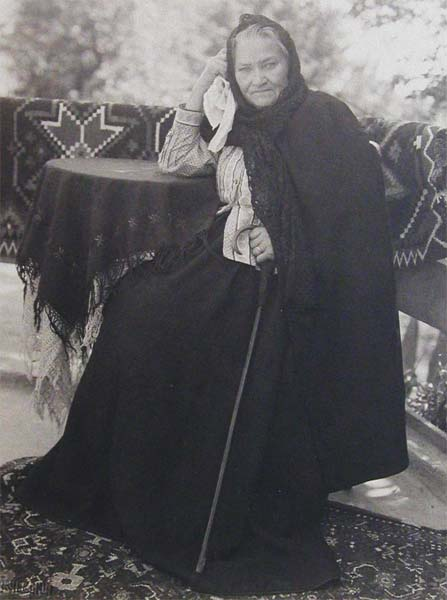
\includegraphics[width=0.98\linewidth]{chast-colebanie-osnov/nachalo/matvienko.jpg}

\textit{На снимке: Феодосия Матвеенкова.}
\end{center}

Между тем в подземелье повалили любопытствующие. Ребятня вытащила несколько черепов, катала по земли – кстати, когда в 1970-х строили крематорий на Байковом и разрушили часть погребений, тоже появились дети, игравшие черепами в футбол.

В пещеру на Ломаковской лазали все кому ни лень, а потом местным это надоело. Каманин пишет, что после заявления в комендатуру жителей усадеб, близких к пещерам, прислали рабочих с лопатами, и те засыпали вход.

По словам Матвеенковой, среди наплыва людей в пещеры был некий профессор Иванов со студентами. Каманин припоминает, что в 80-90 годах 19 века в газете «Киевлянин» проскользнула заметка о том, что неутомимый исследователь древностей и пещер профессор Владимир Бонифатьевич Антонович посетил Зверинецкие пещеры и обнаружил пояса и четки. И что обстоятельному изучению пещер профессором помешало Инженерное ведомство, ибо пещеры находились на территории Зверинецкой крепости. 

Думаю, память подвела Каманина. В 1895 году Антонович выпустил свою знаменитую «Археологическую карту Киевской губернии»\cite{antonovich01}, где по Зверинцу написано ровно следующее:

\begin{quotation}
Предместье Зверинец. Вблизи церкви в 1888 году открыта пещера, служившая вероятно монастырскою усыпальницей. Она представляла широкий коридор в 32 саженя\footnote{68,3 метров.} длиною; в стенах его сделано 48 нишей и в каждой лежало по 2 скелета, у них найдены 2 серебряные креста, несколько бронзовых, кресты плетеные из ремешков, скуфия и остатки обуви.

Киевское слово 1888 г. № 509. Коллекция Хойновского.
\end{quotation}

Как видим, Антонович использует в качестве источника статью из «Киевского слова». Никаких планов пещеры, как кое-кто пишет, в «Археологической карте» нет. Только эта коротенькая заметка.

%Думаю, дело было просто. Когда открыли пещеры, оттуда вытащили всё ценное, что успели – до того, как рабочие пришли и закопали вход. 

Указанные в ней предметы попали в коллекцию археолога Иосифа Адамовича Хойновского (сочинителя очерка «Раскопки великокняжеского двора древнего града Киева, произведенные весной 1892 года»).

В редакции «Киевлянина», где Каманин пытался разы\-скать нужный номер, никто про заметку о пещерах не помнил. А статья в самом деле была, в номере за 12 октября 1888 года – к сожалению, я не смог ее достать. Знаю кратко, что речь шла о провале в земле, возникшем при раскопке склона, где местные брали глину. И дескать открылись «громадные подземные пещеры, напоминающие лаврские».

Каманин много лет сотрудничал с Антоновичем в разных областях, например в создании историко-топографи\-ческих словарей. Но Антонович умер прежде, нежели Каманин начал работу над книгой про Зверинецкие пещеры. Иначе Каманин узнал бы сведения у самого профессора, не прибегая к поискам статьи.

Вы заметили, что Матвеенкова говорила о весне 1882-\-83 годов, а сведения Антоновича относятся к 1888-му?

Николай Петров тоже это заметил в своей брошюре, и нашел другие публикации про пещеры за 1888 год. Он решил, что старенькая Матвеенкова перепутала годы, да вот упустил – Матвеенкова говорила о весне, а вход в пещеры в 1888 году открылся осенью. Матвеенкова перепутала и год, и пору года? Или это два разных «открытия» пещер в северной части Зверинецкого холма?

Петров приводит заметку из «Киевского слова» за 15 октября 1888 года (№ 509) – на которую ссылался Антонович. Петров полагал, что корреспондентом «Слова» был художник Димитрий Зайченко, хотя, даже если не принимать во внимание разницу лет, описания посещения пещеры отличны. В 1882-м лезут двое, в 1888-м трое. Зайченко сам, в полдень, нашел провал, а в 1888-м – сочинителю заметки в 4 часа дня рассказывает о провале знакомый. Судите впрочем сами:

\begin{quotation}
В 4 часа пополудни, 13 октября, до меня дошло известие, что на Зверинце, недалеко от того места, где я живу, открыта новая пещера, и в ней покоятся кости мертвецов. Кем открыта эта пещера и при каких обстоятельствах, никто мне сообщить не мог.

Ко мне подошел живущий на Зверинце К-н и предложил мне идти с ним. Втроем, я, г. К-н и еще один незнакомый мне мужчина, решились спуститься в пещеру, конечно, зажегши предварительно свечи...

При свете свечей, по бокам этой пещеры, в стенах ея с двух сторон мы увидели полукруглые углубленные могилы, где лежали груды человеческих костей, и по два черепа в каждой могиле, причем в некоторых могилах отчетливо видны два человеческих скелета, положенных головой внутрь, а ногами к пещере, так что безошибочно можно заключить,что в каждой могиле находится по два человека.

Пещера оканчивается вертикальной стеной, и в ней находится такая же углубленная могила с двумя человеческими скелетами. Во всей пещере мы насчитали 48 могил, и считая в каждой могиле по два человека, всего будет похороненных 96 человек.

Вся пещера имеет длины приблизительно 96 аршин\footnote{68,28 метров.}. В пещере этой мы нашли два красных кирпича, шириной примерно 1,5 аршина\footnote{1,07 метра.} и толщиной 1 вершок\footnote{4,5 сантиметра.} (длина неизвестная, так как кирпич по длине сломан), уже довольно выветренных, так что рассыпаются, и формой совершенно не похожих на кирпич теперешних образцов, а также нашли кусочки ветхой кожи от обуви.

Больше ничего не оказалось; гробов и следа нет; но в толпе ходят слухи, что будто бы какие-то люди осматривали пещеру раньше и на костях видели уже истлевшее духовное облачение и нашли золотой крестик. 

Болтают также, что будто бы лет 80 тому назад здесь случился обвал и завалил покоющихся здесь. Но это совершенно неправильно.
\end{quotation}

Матвеенкова в 1882 году видела ниши только в правой стене, гробы (хотя бы истлевшие), обитую железом дверь, и трупы головами к выходу из камер. В 1888-м у корреспондента – ниши по обе стороны коридора, никаких гробов и двери, трупы ногами к выходу.

Кажется, в 1882-83 и 1888 году открывались входы в две разные части пещерного комплекса, возможно даже не соединенные между собой.

Петров пишет\footnote{Ссылаясь на «Киевское слово» от 8 ноября 1888, номер 242.}, что прочитав заметку в «Киевском слове», 16 октября 1888 года к пещерам отправились профессор университета Св. Владимира Адриан Викторович Прахов
\footnote{Руководитель росписи Владимирского собора и реставрации Кирилловской церкви.}, художник Т. А. Сведомский да исследователь древностей В. И. Гошкевич.

\begin{quotation}
Профессор Прахов остался на страже у входа в пещеры, а остальные двое отправились в самую пещеру, захватив с собой длинный шнур для сигнализации и для того, чтобы не заблудиться в лабиринте пещерных ходов.

По описанию г. Гошкевича, влево от найденной пещеры виднелась другая пещера, устье которой выходило в нескольких шагах от первого отверстия. Вся длина пещеры около 30 метров. 

К сожалению, за 4 дня со времени ея открытия успело перебывать множество «варваров», окончательно нарушивших первоначальное положение скелетов, так что теперь весьма трудно его определить.

Разрушительная работа велась, по-видимому, таким образом, что не только в самых пещерах все предметы разбросаны, но и содержимое ниш выгребено в пещерный коридор.

В самой пещере Сведомский и Гошкевич встретились с каким-то субъектом, предлагавшим им свои услуги по отысканию могильных предметов.

Но не успели исследователи осмотреть пещеру надлежащим образом, как получили от профессора Прахова предупредительную записочку об угрожаемой им опасности от обвала пещеры, так как над пещерами, в которых находились исследователи, собралась громадная толпа любопытствующих зрителей.

Исследователи благополучно выбрались из пещеры и уже когда двинулись в обратный путь домой, то встретили полицейского, спешившего к месту скопления толпы.
\end{quotation}

Сравним числа. Тут длина пещеры – около 30 метров. А в заметке от 15 октября 1888 года – как мы помним, около 68 метров. Разница слишком велика, чтобы быть ошибкой. В ту ли самую пещеру лазали Гошкевич со Сведомским?

Киевское Военное ведомство отправило в пещеру, посещенную последними, инженера Червинова 2-го. Гошкевич в начале ноября сообщал:

\begin{quotation}
Военным инженером Червиновым 2-м совершена на днях экскурсия в новооткрытую на Зверинце пещеру. Исследование затруднено теперь еще больше по причине происшедшаго в последние дни внутреннего обвала.

Червинову удалось начертить правильный план этого подземелья, с обозначением на нем всех погребальных ниш. Количество их определено им в 36. Так как в каждой нише находится по два скелета (в одной, впрочем, найдено нами 3 скелета), то число всех покойников, погребенных в этой усыпальнице, должно быть не менее 72. Кроме значительного количества лоскутков кожи, других предметов при скелетах г. Червиновым не найдено.

План пещеры, вместе с одним из лучше сохранившихся черепов, будет отправлен в С.-Пе\-тербургский Археологический Институт\footnote{Петров добавляет, что на деле отправили в Императорскую Археологическую Комиссию, а та в 1891 году переслала в Церковно-Археологическое общество при Киевской Духовной Академии, для музея, сандалию из Зверинецких пещер.}.
\end{quotation}

36 ниш против 48 из заметки за 15 октября. Спишем на обвал, или – таки другая пещера?

Затем Зверинецкие пещеры выпадают из поля зрения ученых и общественности до 1911 года,  когда снова провалилась земля и открылось два новых входа. Каманин пишет, что 30 лет эти пещеры «находились без охраны», Эртель говорит про 20 лет – однако если в 1911 году пещеры вновь «открылись», значит, старые входы были завалены (нет и точных сведений об их месте). О каких же 20 или 30 годах разорения пещер идет речь? Вход 1882-го, по сведениям Каманина, закопали власти. Судьба входа 1888 года теряется в истории.

%Тогда-то и началось масштабное изучение пещеры Эртелем при содействии князя Жевахова.

Каманин (совмещая, как я считаю, два обнаружения пещер 1882 и 1888 годов в одно событие) полагал, что Матвеенкова попадала в какую-то другую пещеру (или часть), не ту, где рыл Эртель и примкнувший к нему позже Вельмин. Так можно судить по описаниям, оставленным последним, и показаниям самой Матвеенковой, которая уже при Эртеле, когда ее повели под землю, не узнала пещеру. Найденные тридцать лет назад ею пещеры – «это не те пещеры, которые теперь раскопаны – это другие пещеры, до которых еще не докопались. Надо копать в правую сторону, более под мою усадьбу».

По Сети бродят сведения без источника, что георадиолокация показывает еще около километра неизвестных пещер. В одном из коридоров Зверинецких пещер – «Погребальной улице» – есть завал, где через десять метров прощупывается пустота – и вот что за этим завалом, пока неведомо. Вероятно это те самые исследования, которые производились Институтом прикладных проблем экологии, геофизики и геохимии в 2001 году, из коих мне известно следующее – в ботсаду и по Мичурина 10, 12 и 14\footnote{Мичурина 10 – это не Ломаковская 10, нумерация сильно сдвинулась. У меня нет уточняющих данных, но как я понимаю, участок ботсада с пустотами примыкает к упомянутым усадьбам. В ботсаду там растут огромные акации.} показали на площади 65x115 метров наличие там «аномальных зон», которые трактовали как подземные пустоты. Проверяли ли дальше на юг, номер 8 и местность Собачку, я не знаю. Но от жителей усадьбы номер восемь я слышал только историю о живущем на чердаке домовом, а про пещеры ничего не слышал, равно как не замечал их на Собачке, прожив рядом добрые двадцать лет.

Эртель во время раскопок 1912 года увидел, что от Зверинецких пещер в сторону Ионинского монастыря идет подземный ход, и предположил, что всё пространство между монастырем и Зверинецкими пещерами изрыто ходами, но там находился Зверинецкий форт, под который копать было невозможно\footnote{К слову, когда в ботсадовском Розарии (лежит в пределах бывшей крепости) вместо нынешнего центрального бассейна было озеро с земляными берегами и фонтанами (по плану ландшафтного архитектора Рубцова), вода просто уходила в какие-то подземные пустоты. Даже когда в 1970-х забетонировали дно и построили каменные бортики, вода продолжала уходить.}. Эртель также нашел провалы в несколько отдаленной от раскопок усадьбе зубного лекаря В. Шмигельского и подумал, что под ними тоже части пещерной сети. К слову, по северной и западной возвышенной части горы Эртель заметил древний вал и сопоставил его с упоминаемым в летописи Красным двором Всеволода Ярославича. Там где сейчас в ботсаду воссоздан «Красный двор» в самом деле кромка склона издревле несет следы земляных работ, а под тамошним обрывом я находил плинфу – древнерусский кирпич. Мыс с обрывом именуется «мыс Чайка». Название, по одной версии, от бывшей тут дачи профессора-уролога Андроника Архиповича Чайки, а по другой версии - от фамилии капитана красноармейcкой батареи, стоявшей здесь во время Великой Отечественной войны.

В 11 номере «Киевской мысли» за 1913 проскользнули упоминания о втором ярусе пещер (их же повторил в виде предположения Шероцкий в газете «Рада», №2 за 1913 год), над открытыми, и о провалах возле Ионинского монастыря\footnote{Около монастырской ограды археолог Стеллецкий позже нашел некий подземный лабиринт, и выразил мысль что всё это часть единой со Зверинецкими пещерами подземной системы ходов.}, и что один такой провал забирает всю весеннюю воду. В 29 номере «Киевлянина» за 1913 тоже есть про второй ярус пещер, причем если Шероцкий полагал что он находится над уже раскопанными ходами, в «Киевлянине» речь идет о нижележащем этаже:

\begin{quotation}
Недавно в галерее, соединявшей старый и новый выходы из пещер, приблизительно в средней ее части обнаружена небольшая лазейка, за которой замечена круглой формы небольшая комната. В ней имеются ясные признаки заваленного хода – спуска. Возможно, что это спуск во второй ярус пещер, о котором местное население давно говорит и куда некоторые местные старожилы уже проникали несколько лет тому назад и по их описанию эти пещеры имеют иной вид, нежели открытие пещеры. Там были сравнительно большие комнаты, находились части облачений, ручные кресты и другие предметы.

Рассказы о существовании второго нижнего ряда галерей и пещеры находят себе некоторое подтверждение в существовании провалов на поверхности всей площади, направление которых не совпадает с открытыми уже галереями, но почти тождественно с направлением пещер, о которых говорят местные жители. Между тем на этой площади, как мы слышали, предполагается постройка больших воинских казарм.
\end{quotation}

...Как известно, поныне раскопан только один ярус.

В 1911 году набожный князь Владимир Жевахов (будущий Иоасаф, архиепископ Могилевский) взял в аренду на 6 лет участок земли в 350 квадратных сажень (746,8 кв. метров) с новооткрытыми пещерами и организовал там раскопки. Позже Жевахов ходатайствовал о передаче этого участка и окрестностей духовному ведомству, но военное ведомство отказало, ибо собиралось строить там казармы для частей Киевского гарнизона, и посоветовало арендовать взамен соседнюю частную усадьбу.

\begin{center}
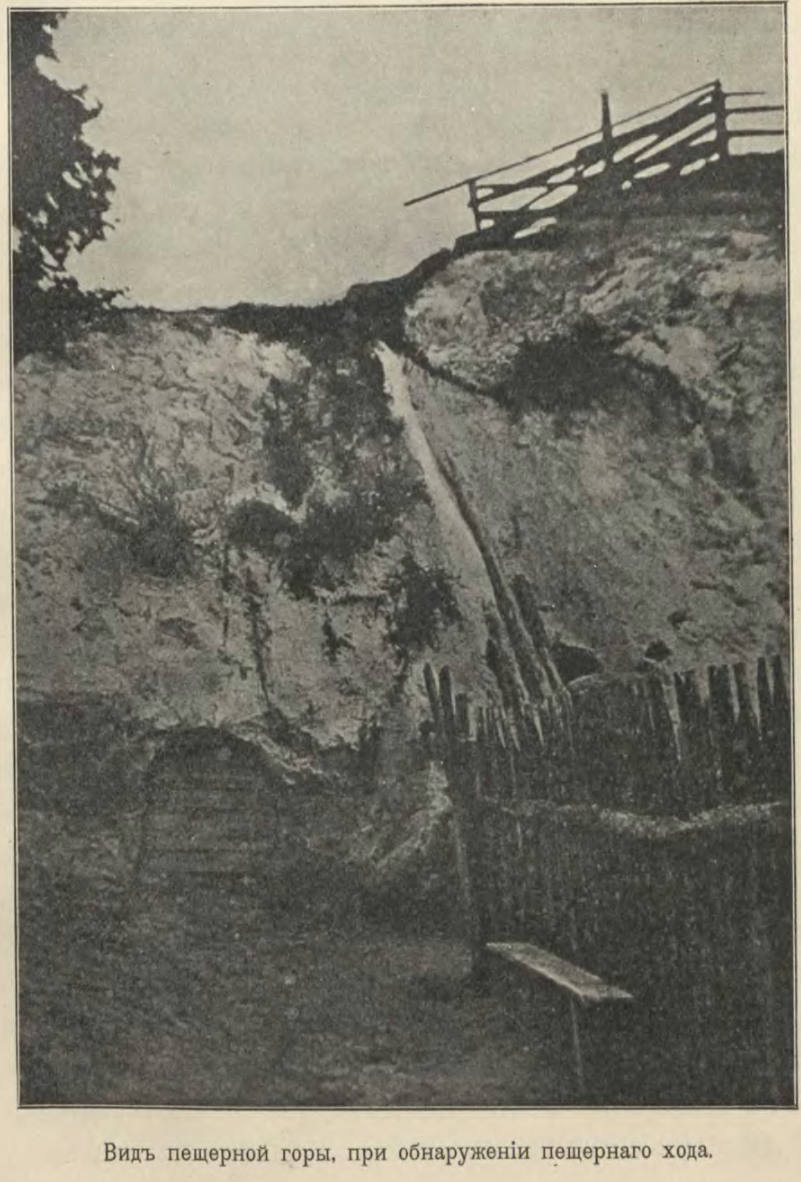
\includegraphics[width=0.90\linewidth]{chast-colebanie-osnov/nachalo/zverp-02.jpg}

\textit{Снимок 1911 года.}
\end{center}

\newpage

Петров осторожно пишет:

\begin{quotation}
О новооткрытых пещерах узнал проживавший тогда в Киеве князь Вл. Д. Жевахов, тот самый, который, вместе с братом своим Николаем, так сильно хлопотал об открытии нетленных мощей и канонизации своего родственника по женской линии, святителя Иоасафа Горленка, епископа Белгородского.

Князь задумал открыть Зверинецкие пещеры не столько как памятник глубокой древности, сколько как народную святыню, и сделать их доступными для народного поклонения и чествования. Этою религиозною целию забот князя Жевахова нужно объяснить то обстоятельство, что он обратился за разрешением работ не к Императорской Археологической Комиссии, ведающей все находки и раскопки древностей, а к духовному начальству, хотя не пренебрегал совершенно и научными интересами. Осенью 1911 года он взял в аренду у Инженерного ведомства тот участок земли, на котором находились Зверинецкие пещеры, и попросил благословение на открытие пещер у Киевского Митрополита Флавиана, которому князь сообщил о пещерах письмом. Наместник Киевопечерской лавры архимандрит Амвросий предложил заняться раскопкою этих пещер секретарю Киевского Общества Взаимного Кредита А. Д. Эртелю.
\end{quotation}

Раскопки начались только в июле 1912, поначалу даже без Эртеля – тот был занят в Китаевских пещерах, полагая в последних начало древнего Киева.

Копия рапорта Киевского полицмейстера от 28 июля 1912 года за № 9951 на имя Киевского Губернатора.

\begin{quotation}
На арендуемом князем Жеваховым от инженерного ведомства участке земли, находящемся сзади № 10 по Ломаковской улице производится богомольцами-охотниками\footnote{Т.е. желающими, добровольцами.} под руководством рабочаго крестьянина Семена Гончарова раскопки в целях открытия древних пещер-усыпальниц. 

%В настоящее время под горой Печерскаго укрепления открыт вход в пещеру, оказавшуюся в измерении 3 1/2 аршина\footnote{2,5 метра.} в квадрате, а из нея в глубь горы имеется ход в виде корридора шириною 2 арш. 2 вершк.\footnote{1,48 метра.}, вышиной 1 арш. 2 вер.\footnote{0,8 метра.} и длиною 41 аршин\footnote{29,2 метра.}, в нем обнаружено 32 места, где, повидимому, находились гробы с телами, на что указывают найденные остатки человеческих костей.

В настоящее время под горой Печерскаго укрепления открыт вход в пещеру, оказавшуюся в измерении 3 1/2 аршина в квадрате, а из нея в глубь горы имеется ход в виде корридора шириною 2 арш. 2 вершк., вышиной 1 арш. 2 вер. и длиною 41 аршин\footnote{2,5 метра в квадрате, 1,48 метра ширина, 0,8 метра высота. 29,2 метра длина.}, в нем обнаружено 32 места, где, повидимому, находились гробы с телами, на что указывают найденные остатки человеческих костей.

Раскопками заведует игумен Свято-Троицко\-го монастыря о. Валентин. 

Об этом доношу Вашему Превосходительству. Подлинное за надлежащими подписями.

С подлинным верно: Правитель Канцелярии Киевскаго Губернатора (подпись)

Сверял: Помощник Правителя (подпись)\end{quotation}

Мысленно потираю руки – обсудим! Вот у нас появился адрес пещер – участок земли позади усадьбы номер 10. Как мы знаем, на самой Ломаковской, 10 жила Матвеенкова. Ломаковская теперь называется Мичурина, и 10-й номер по Мичурина это, на 2016 год, частный дом, стоящий под горкой на той же стороне улицы, где и Зверинецкие пещеры, которые ныне имеют адрес Мичурина, 20-22 (в 1998-м: 18-22). От номера 10 до 20 около 150 метров. Значит, старая и новая нумерация не совпадают. Сравним теперь числа «от Матвеенковой» 1882 года, 1888-го и 1912-го.

У Матвеенковой – 50 гробов в отдельных пещерках по правой стене, по два тела в каждой могиле. И значит, 50 ниш в одной только стене. А другая, стало быть, без ниш.

1888 год, в первой заметке от неизвестного корреспондента – «по бокам пещеры» 48 могил с двойными погребениями. В одной из последующих заметок, уже в пещере, где побывали Прахов, Сведомский, Гошкевич и Червинов 2-й – 48 могил, при этом неясно, по одной стороне коридора или обеим.

Наконец 1912 год, первые раскопки – 32 ниши, и согласно позднейшим планам пещер – в каждом коридоре ниши были по обе стороны.

Затем раскопками стал руководить Эртель, поставив дело на научную основу. Кроме прочего он составил план расчищенного им участка пещер, несколько позже другой план начертил В. В. Кузнецов, сотрудник покойного к тому времени археолога Д. В. Милеева.

Перед разбором планов опишу рельеф местности. Северо-восточный, клиноподобный угол Зверинецкого холма. Сверху вниз – крутой склон (со входом в пещеру у его подножия), терраса с Ломаковской улицей, затем более пологий склон. Вдоль улицы, с течением времени, верхний крутой склон террасировался для разбивки там садов и огородов частного сектора.

\begin{center}
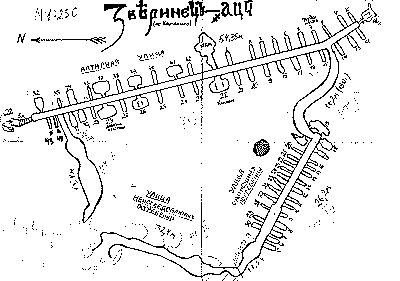
\includegraphics[width=0.90\linewidth]{chast-colebanie-osnov/nachalo/zverp-plan01.jpg}

\textit{Один из планов пещер, открытых в 1911 – еще не прорыт соединительный коридор для удобства паломников.}
\end{center}

\newpage
\vspace*{\fill}

\begin{center}
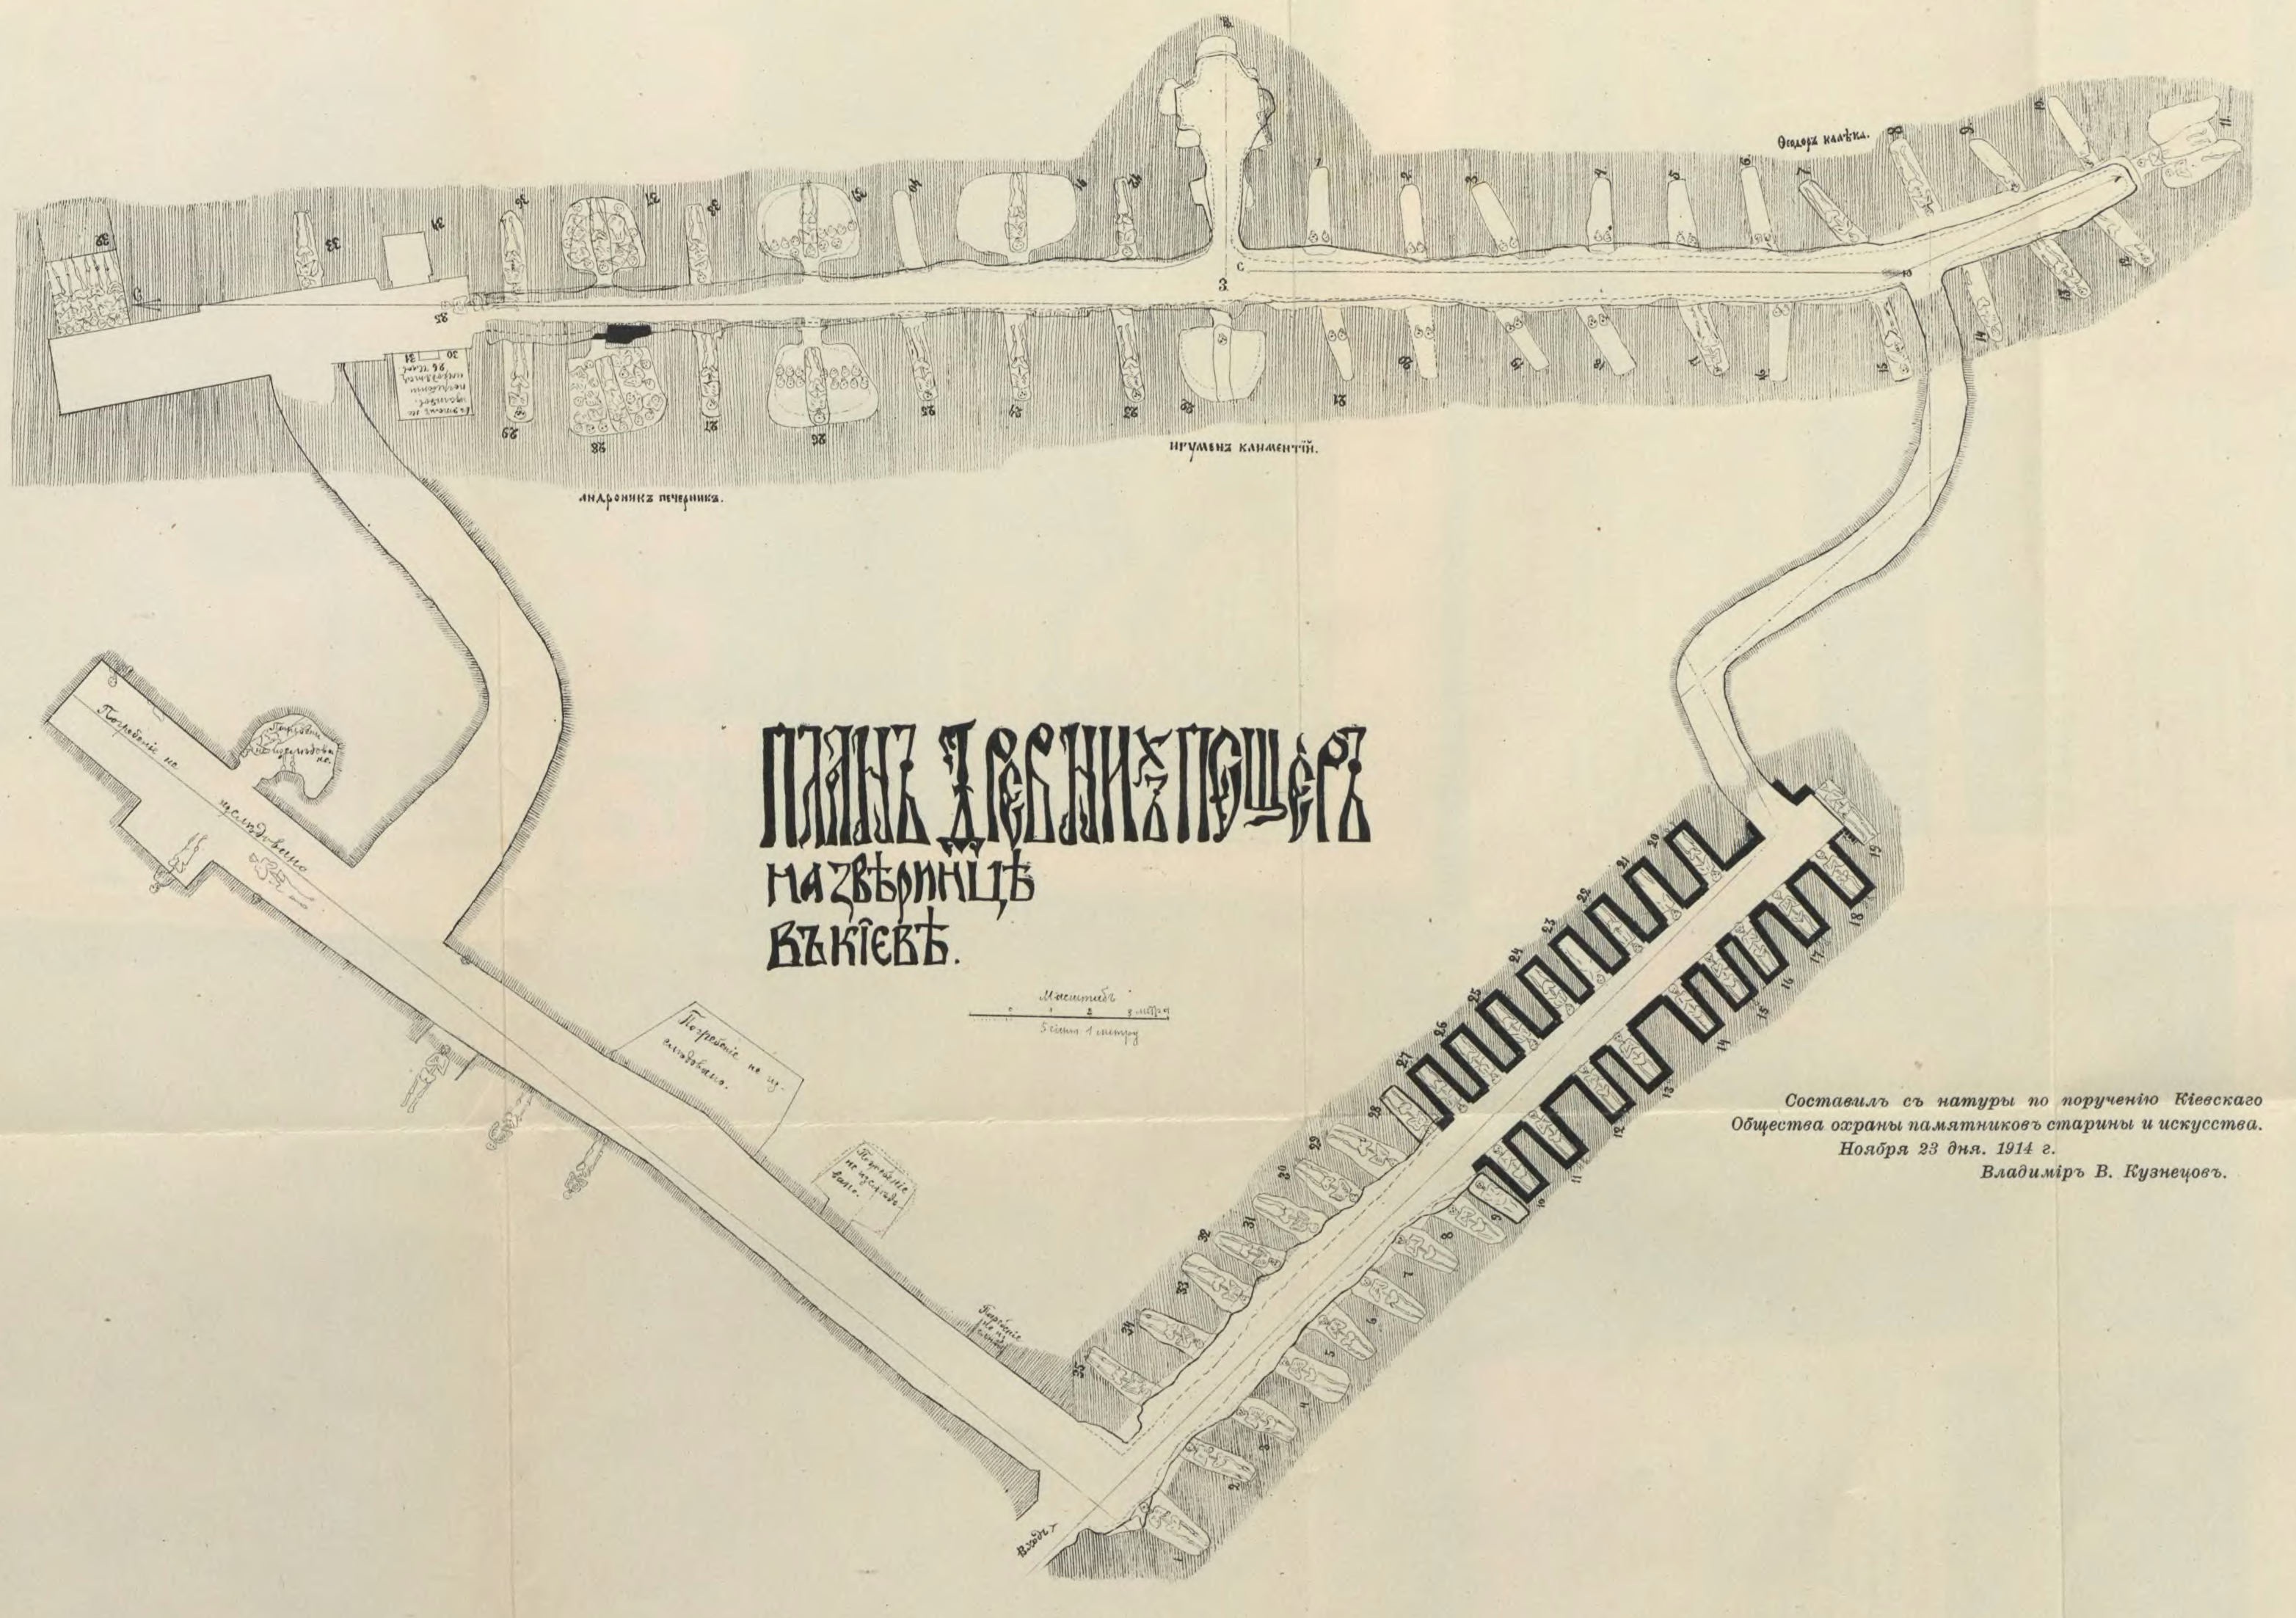
\includegraphics[width=\linewidth]{chast-colebanie-osnov/nachalo/zverp-plan02.jpg}

\textit{План Кузнецова. Современный вход – слева сверху.}
\end{center}

\begin{center}
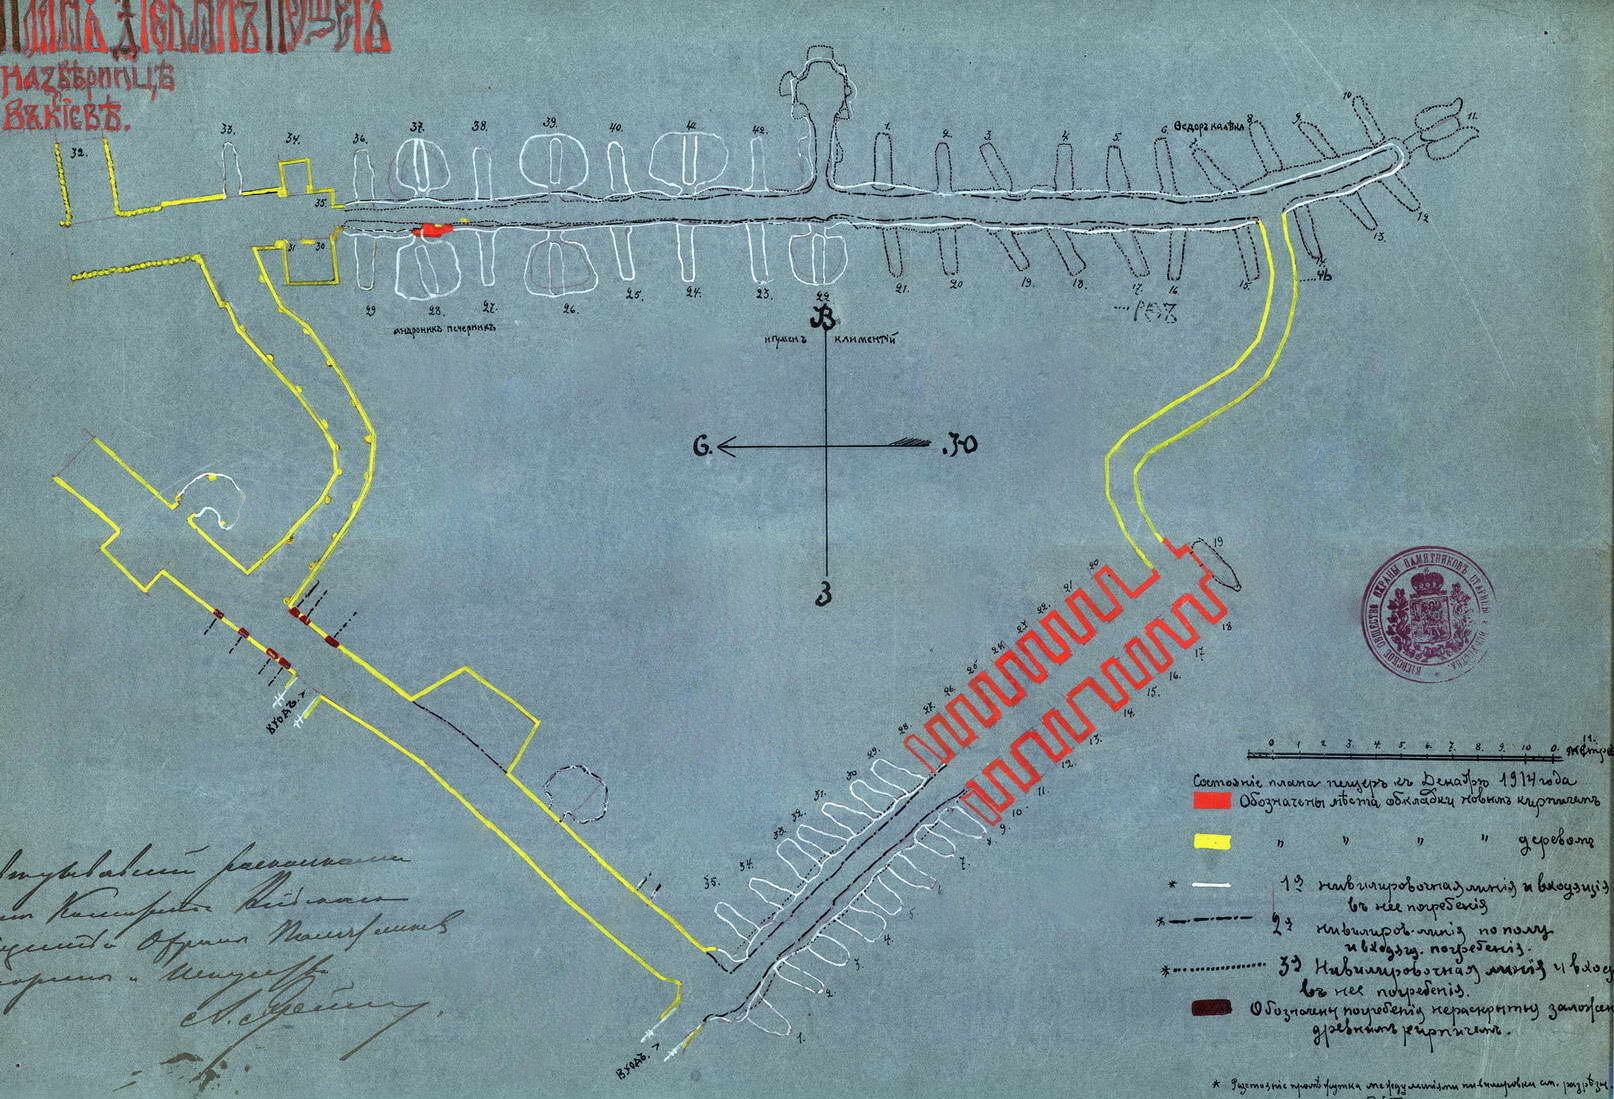
\includegraphics[width=\linewidth]{chast-colebanie-osnov/nachalo/1914-ertel.jpg}

\textit{1914. План с подписью Эртеля.}
\end{center}

\vspace*{\fill}
\newpage

Пять коридоров («улиц»), взаимное расположение которых образует треугольник. Разница между планами – пара лет, однако на втором видно, что прорыли коридор, соединивший северные части двух улиц.

Где находился изначальный вход 1911 года, не вполне ясно, однако на плане Кузнецова вход – посередине внизу плана, и на другом плане 1914 года появляется второй вход едва не на месте погребений. Современный же, 21 века вход – в верхнем левом углу.

%Очевидно, что подземелье было вырыто по начертанному ранее проекту, и в ходе работ использовались какие-то измерительные средства, позволившие придерживаться начального чертежа.

Обмеры коридоров, по Кузнецову, таковы. Правый от тогдашнего входа («улица одиночных погребений») – длина 26,20 метров (13 сажень), на одной стороне 18 ниш, на другой 16, одна в тупике, всего 35, погребения одиночные. Левый («улица неисследованных погребений») – 32,40 метра (19 сажень). Поперечный коридор («алтарная улица») – 54,35 метра (27 сажень), по стенам расположены комнаты с массовыми погребениями (останки более двух людей в одной келье), и около трех десятков двойных (скелеты лежали друг на друге) и одиночных погребений.

Говоря о кельях, которых на Алтарной улице насчитали три, Каманин сообщает, что «высота всех келлий общая с высотой пещер, от 1,80 до 2 метров». Пещеры, куда лазала Матвеенкова, имели высоту 2,1 метра.

Но вот газета «Киевлянин» в № 55 за 24 февраля 1913 года поместила заметку про доклад Эртеля и Каманина в феврале 1913 года на заседании Исторического общества Нестора-летописца. Выдержки оттуда, касаемо доклада Эртеля:

\begin{quotation}
На первых порах при зверинецких раскопках пришлось преодолеть некоторые затруднения: пещеры привлекли огромные массы паломников со всех концов Руси; своим любопытством они мешали работам, которые и без того требовали большого внимания и осмотрительности: возможен был обвал и за рабочими приходилось тщательно наблюдать.

Все это осложнялось еще спором о казармах, которые предполагалось строить на месте производства работ, по раскопкам. Сейчас раскопки далеко еще не закончены, но в некоторых местах подошли уже к границам частных усадеб.

Пока отрыты несколько низких (в них нельзя выпрямиться) длинных галерей со множеством усыпальниц, из которых большинство разрушено.
\end{quotation}

А почему Каманин в своей книге пишет о высоких потолках? Где же эти галереи, в которых нельзя выпрямиться? Читаем «Киевлянина» дальше:

\begin{quotation}
Кирпич, найденный здесь, относится к XI и позднейшим векам. Встречаются кирпичи, бывшие, очевидно, уже в употреблении и принесенные сюда из других построек. 

В конце одного хода обнаружены несколько скелетов, расположение которых наводит на мысль о какой-то драме, быть может, времен татарщины.

В центре открытой системы галерей (система незаконченная, неясная, что заставляет предполагать существование 2-го яруса подземных ходов) находится низкая четырехугольная камера, с нишами в северной и восточной стенах, где, предполагает докладчик, находились жертвенник и престол этой подземной церкви. вмещавшей не более шести человек.
\end{quotation}

Заметим предположение о втором ярусе пещер, краткие сведения о «драме», и указание на низкую камеру с жертвенником. Это же помещение по обмерам из книги Каманина становится если не просторнее, то по крайней мере несколько выше – два метра.

Посмотрим на выполненный Кузнецовым план Алтарной улицы в разрезе, 1914 года – все обмеры указаны в сажнях, а сажень это примерно 2,1 метра. Вид с востока:

\newpage

\vspace*{\fill}

\begin{center}
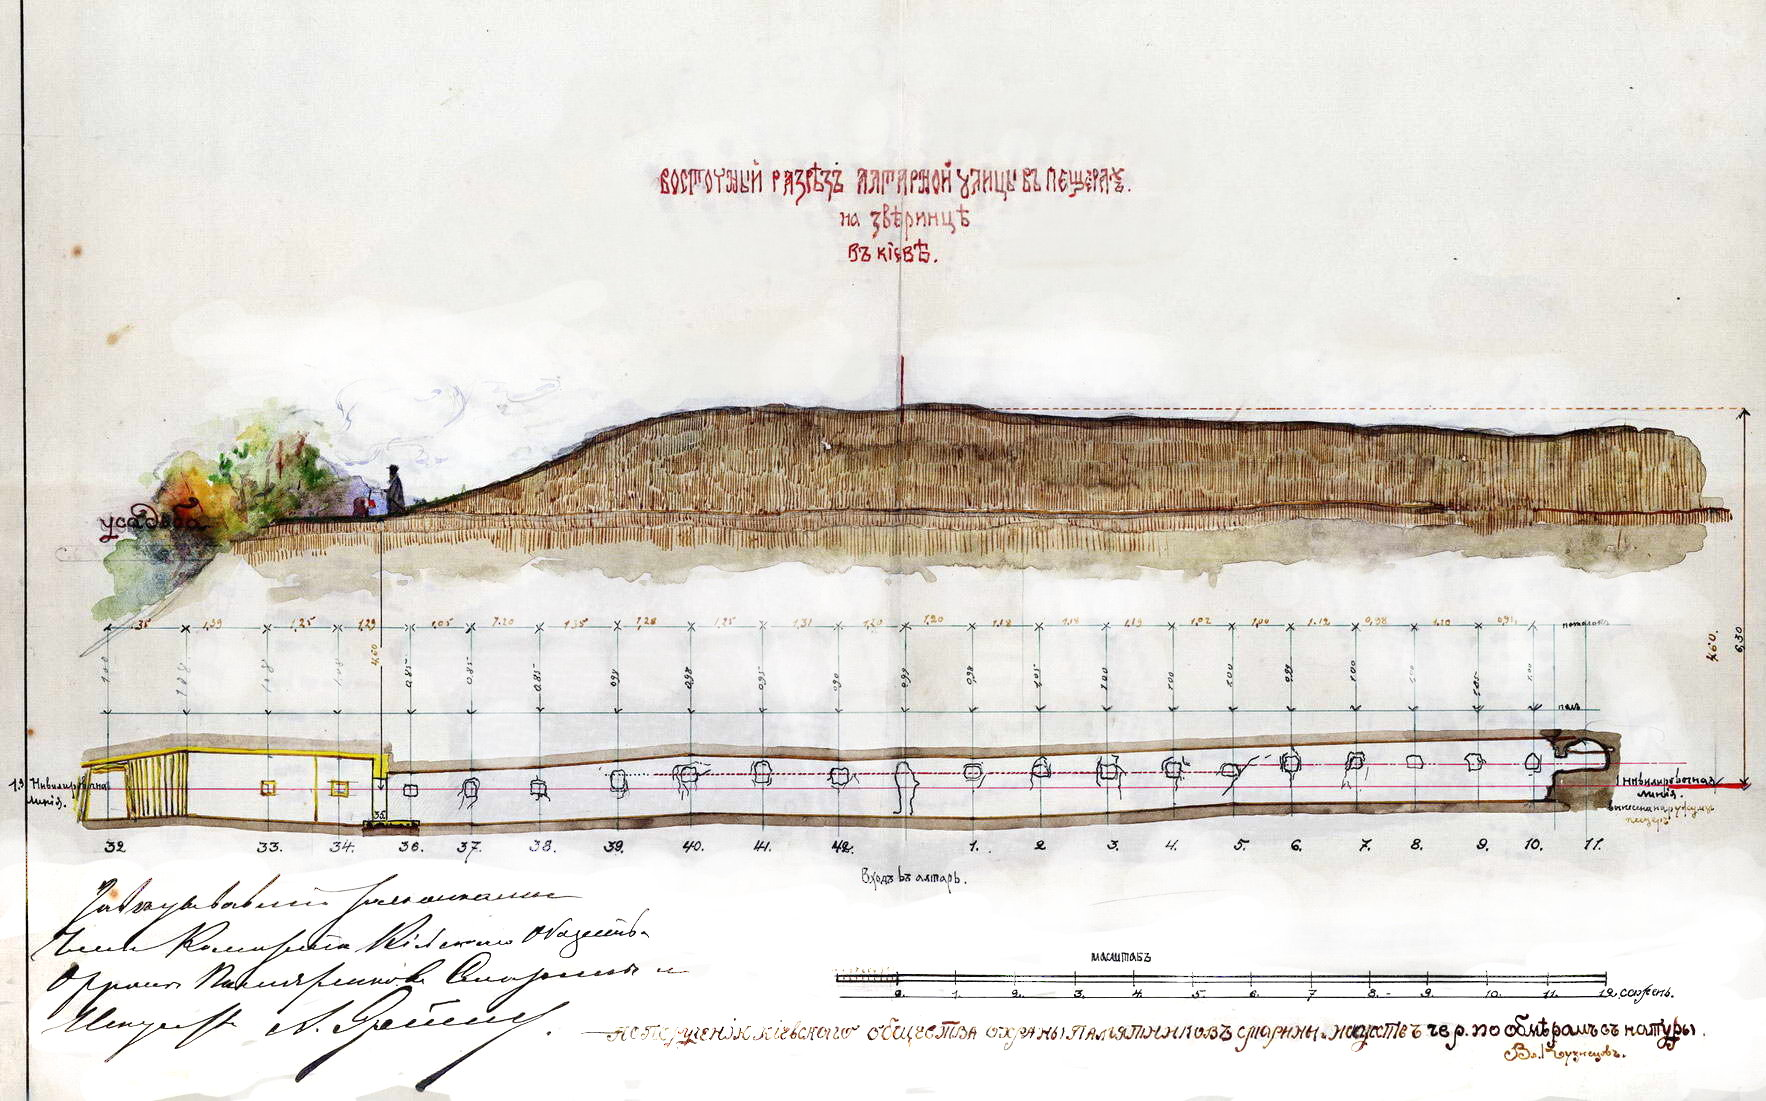
\includegraphics[width=\linewidth]{chast-colebanie-osnov/nachalo/1914-01.jpg}
\end{center}

\vspace*{\fill}

Над коридором изображена шкала, где для каждого участка по оси X отмечена его длина, а по оси Y – высота потолка.

Посередке обозначен «Вход в алтарь». Какая высота потолка? 0,99 сажени – это таки около двух метров.

Со времени доклада Эртеля потолок подрос? Судя по данным высот с этого же «разрезного» плана, нигде в Алтарной улице не нужно идти пригнувшись.

Что кстати еще полезного можно узнать из плана? Видите две фигуры на пригорке – черную и в красной шапке? Эти люди пробурили в коридор шахточку, и высота ее составила 4,60 сажни, это 9,66 метра. Ниши в коридоре пронумерованы до 42.

Познакомимся с разрезом «Второй улицы» («одиночных погребений») с запада, причем на плане отмечены только ниши, находящиеся по правую руку, если смотреть от обозначенного на нем входа (тоже справа). Всего же ниш – 35.

Масштаб указан уже не в сажнях, а в метрах – вероятно, обмеры тоже в метрах.

\begin{center}
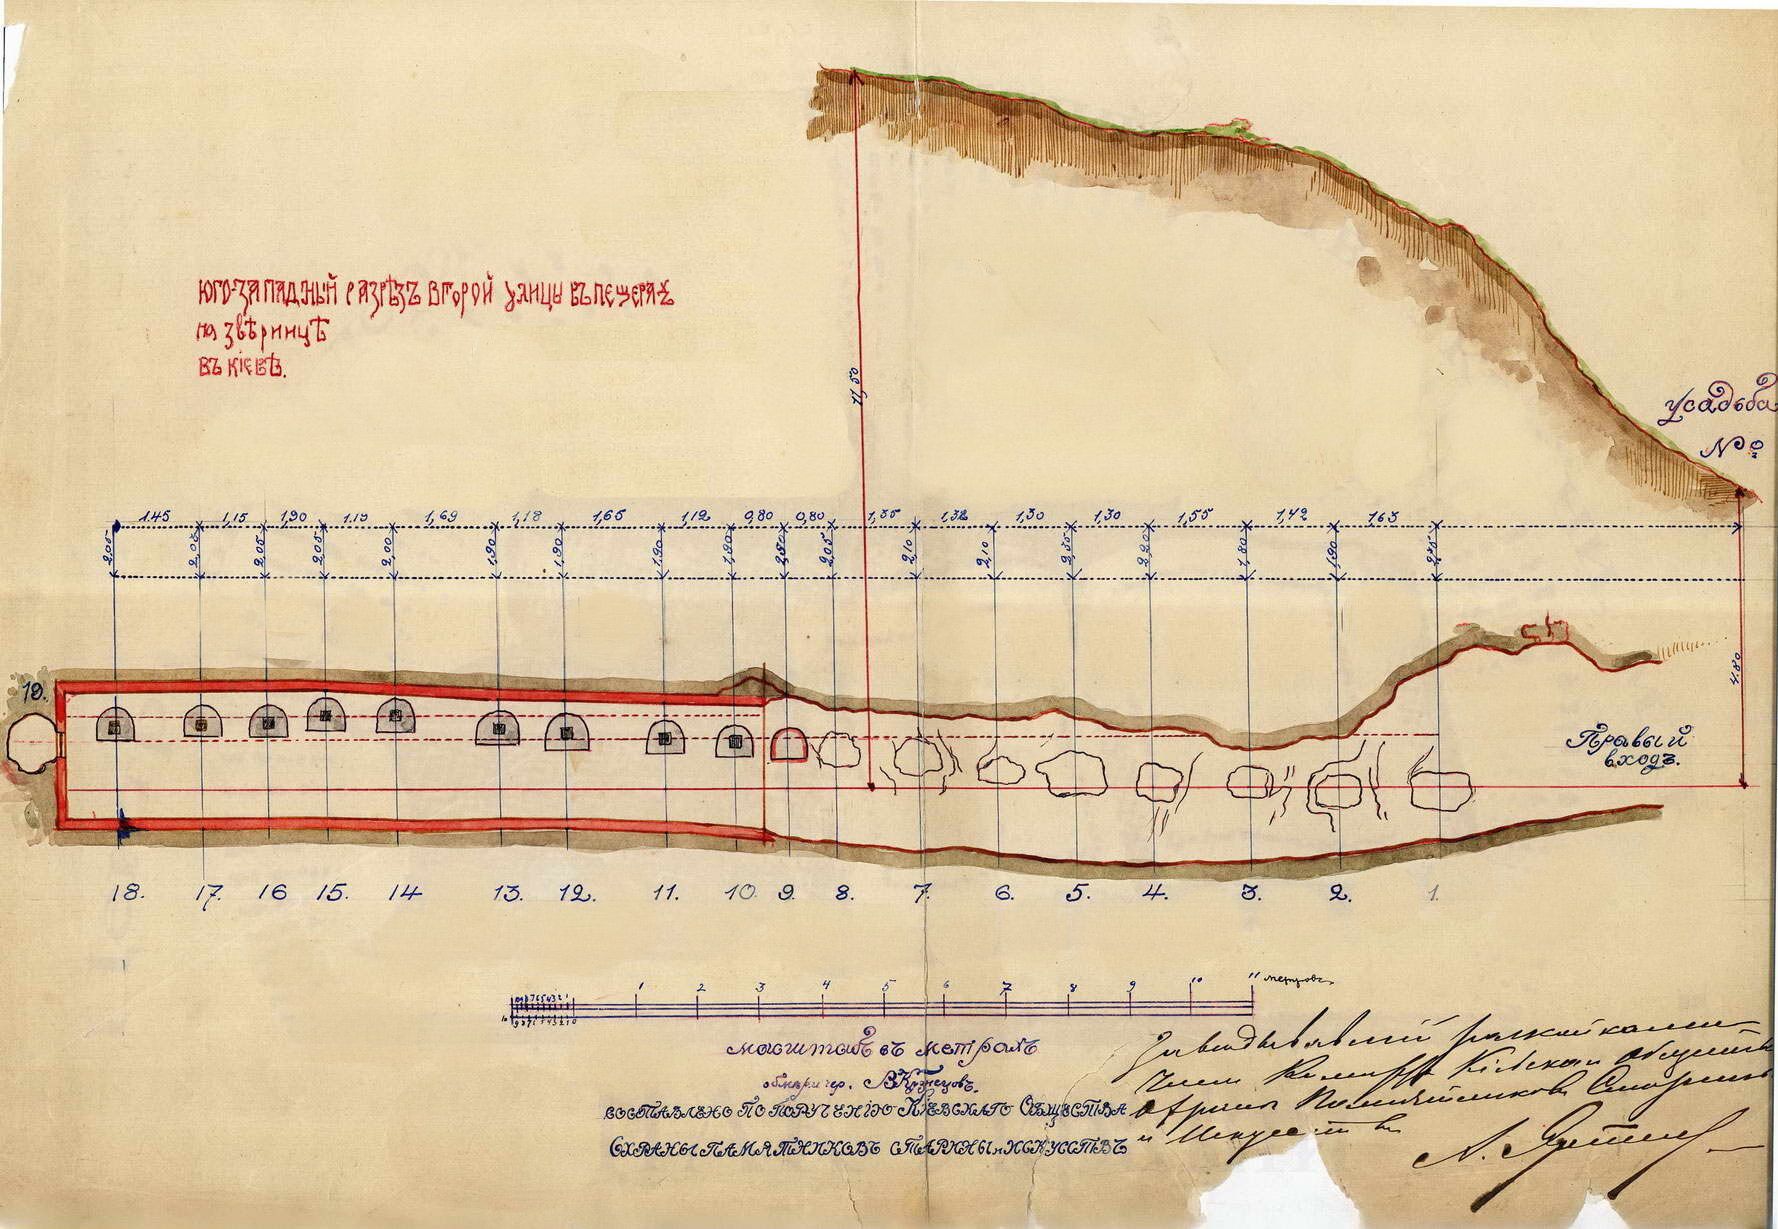
\includegraphics[width=\linewidth]{chast-colebanie-osnov/nachalo/1914-02.jpg}
\end{center}

То, что числа выражают метры, подтверждается указанной глубиной залегания коридора – 11,50 от поверхности. Если Алтарная улица лежала в 9,66 метрах, то 11,50 – сопоставимая величина, ведь если бы 11,50 было в сажнях, это даст нам глубину более 20 метров. А поскольку оба коридора лежат примерно на одном уровне, значит, 11,50 – именно метры.

Может быть это низкий коридор, где нельзя разогнуться? Да вроде бы нет, один только участок 1,80 метра, остальные 1,90 и даже более 2 метров. 

А как же данные самого начала раскопок? Когда

\begin{quotation}
а из нея в глубь горы имеется ход в виде корридора шириною 2 арш. 2 вершк., вышиной 1 арш. 2 вер. и длиною 41 аршин, в нем обнаружено 32 места, где, по-видимому, находились гробы с телами
\end{quotation}

Здесь высота потолка – 0,8 метра, длина около 30-ти. 32 ниши против «официальных» 35 с плана Кузнецова. Будто тот же самый коридор, да вот только высота потолка снова стала много выше. 

Воистину чудесны киевские пещеры! 

Из подземного хода, где надо ползти на карачках, всего за пару лет образуется удобный для пешего хождения коридор.

Сам Эртель в книге 1913 года писал про «улицу одиночных погребений» следующее:

\begin{quotation}
Правый ход (А) ведет в длинный коридор, в котором по обе стороны расположены одиночные и двойные усыпальницы, к сожалению, все разрушенные и разграбленные. В них остались только разбросанные в беспорядке кости, часть которых, по-видимому, унесена или перенесена в другое место. Кости – плохой сохранности, и некоторые совершенно рассыпаются.

Усыпальницы расположены так густо, что промежутки между ними занимают не более полуаршина. Местами сохранились обломки почти совершенно истлевших деревянных досок (по-видимому дуб), но были ли тут гробы, определить с уверенностью нельзя.

Ход в общем широкий, но низкий, так что почти везде нужно идти согнувшись.
\end{quotation}

Низкий ход... Идти согнувшись... А согласно плану – средняя высота потолка около двух метров!

В докладе на заседании общества Нестора-Летописца говорилось, что останки, вид которых намекал на некую трагедию, лежали в конце коридора. Каманин же сообщает в книге, как свидетельство внезапной гибели людей, что часть скелетов, лежала на полу коридоров, и много ближе ко входу, в беспорядочном положении.

Как бы ни было, это можно толковать двояко – люди погибли и остались на месте смерти, либо же их останки переместили уже после, например при разграблении пещер.

Некоторые ниши-усыпальницы были заложены кирпичом (датированным 11 веком, однако вроде были и позднейшие). Эртель нашел также кирпичные плиты, похожие на части круглых колонн. Предметы из кожи – плетеные кресты, остатки обуви, а также поясов с названиями либо оттисками изображений христианских праздников (в прямоугольных рамках до трех сантиметров в ширину, около двух в высоту, видны распятие Христа, въезд его в Иерусалим на «жребяти осли», воскресение Лазаря, и тому подобное), несколько черепков.

\begin{center}
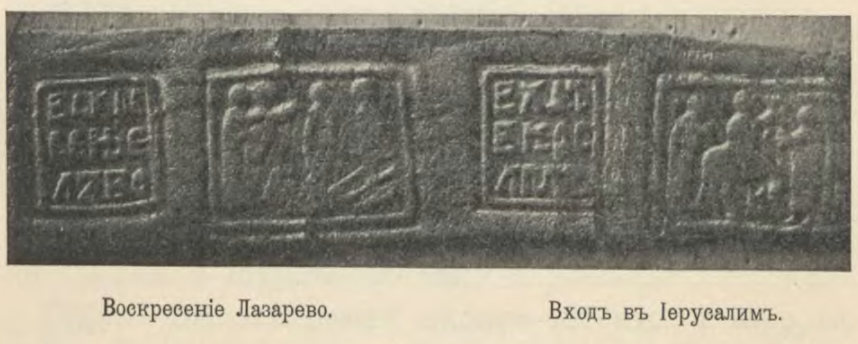
\includegraphics[width=\linewidth]{chast-colebanie-osnov/nachalo/poyasa.jpg}
\end{center}

%\begin{center}
%\includegraphics[width=\linewidth]{osn-kiev/poyasa02.jpg}
%\end{center}

По находкам Эртель судил, что подземный монастырь существовал в 12, 13 и 17 веках. Непрерывно или временами?

Описание пещер 1911 года открытия кажутся мне отличными от пещер открытия 1882 и 1888 годов, на что указывают хотя бы числа – длины коридоров и связанные с ними количество и виды захоронений (одиночные, двойные, массовые), наконец сведения о нишах только справа – у Матвеенковой.

%В статье про Зверинецкие пещеры из сборника «Звід пам'яток історії та культури України. Київ» 1999 года издания, где все местные подземелья смешали в одну кучу, упоминаются еще некие исследования 1990-х, 

Насколько я знаю, в пещерах допустим Лавры – лишь одно «двойное» захоронение, Паисия и Меркурия, кои, будучи дружны при жизни, были по их же просьбе положены в одном гробу посмертно, как повествует «Патерик Печерский».

Что за странные похоронные обряды в Зверинецких пещерах? И чьи скелеты найдены в коридорах?

По 1980-е укрепилось мнение, что это был обычный пещерный монастырь со своими захоронениями и вполне живой братией, где случилась какая-то трагедия. Десятилетие спустя, после исследований пещер под руководством Елены Воронцовой, возглавлявшей тогда отдел «Киев подземный» Музея Истории Киева, предположение науки о «трагедии» вроде бы пошатнулось и эта шаткость даже проникла в поверхностную статью из сборника «Звід пам'яток історії та культури України. Київ» 1999 года издания, однако я не знаком с итогами этих исследований в полной мере, и доводами против того, что лежащие на полу скелеты не могут свидетельствовать о насильственной смерти.

По какой-то же причине Зверинецкие пещеры были заброшены на века.

%Каманин пишет о монахах, хотя предполагает, что это могли быть и кости каких-то укрывшихся в пещерах местных жителей. 

%Ежели первое, то – произошло нечто страшное, и в пещерах все погибли, никто не вышел. От чего погибли? Исследования не проводились.

Есть домыслы – мол, на окрестности напали враги (обычно Половцы), а местное население укрылось вместе с монахами в пещерах и крепко держало оборону в узких коридорах, поэтому лиходеи просто засыпали вход. Тогда почему погребенных заживо не раскопали современники?

Выходит, все, кто знал о пещерах, в них и погибли? А может, по некой причине, пещеры никто не хотел раскапывать на протяжении веков.

И неведомо же, когда именно умерли люди, и спустя какое время вход или входы оказались засыпаны, а также как засыпаны – людьми ли, либо случился естественный обвал.

Во время раскопок пещер в начале 1990-х, заказали изучение останков группе медиков. В нее вошли профессор кафедры рентгенорадиологии Национального Медицинского Университета Татьяна Топчий и студенты Р. Л. Новакович, С. В. Дудник, В. В. Столяров.

Они исследовали останки из 78 раскопанных ниш. 1721 целая кость, 5000 кусков костей – всё, что уцелело, по прикидкам, от 200 человек, из коих взрослых было 145, и 53 детей до 15 лет (в том числе 3 – новорожденные, 2 – младенцы до 1 года, 7 – 1-2 лет). 5 захоронений оказались женскими. За числами стоят живые когда-то люди, они разговаривали, ходили, смеялись.

Целых черепов не сохранилось, и медики не смогли определить расы погребенных. О возрасте судили по стёртости зубов (таковых пригодных черепов оказалось 11) и костям, вычислили средний возраст – 45-55 лет, наибольший – 80 и старше. Средний рост составил 116,33 сантиметров, плюс-минус 7,3. Хотя некоторые мужчины были по два метра.

Кости датировались по виду. Часть отнесли даже к 20 веку, а старейшие – к домонгольскому периоду. Каким образом? А вот, в Лавре есть мощи летописца Нестора. Он ведь до «монгольского нашествия» жил? Давайте, говорят эксперты, сравним цвет и степень сохранности «зверинецких» костей с костями Нестора. Если похожи, значит они тоже домонгольского периода.

Некоторые кости имели необычный вид, а также наросты, что исследователи пояснили тяжелой жизнью в пещерах. Удивила дугоподобная грудина. Сие, по мнению медиков, означало наличие стеноза устья аорты – «сердечный горб».

Смешанность погребений – разных полов и возрастов – пояснили тем, что местные жители знали о пещерах и использовали их в качестве кладбища.

К сожалению, я не обладаю подробностями б\'ольшими, чем изложил (опустил лишь сведения о сросшихся переломах и остеохондрозе у некоторых покойников).

Теперь обсудим. Начну с конца. 

В народе всегда придерживаются традиций погребения. В обозримом прошлом, на Киевщине, простые люди хоронили своих умерших в земле или сжигали, а прах в глиняных сосудах опять-таки закапывали. Пещерные же захоронения совершались служителями культа для своих собратьев, и в Киеве погребальных пещер было не столь уж много.

В христианское время, вне кладбища хоронили только некрещеных детей, самоубийц, колдунов, опойц и умерших насильственной смертью – относительно последних этот обычай к 19 столетию отжил.

С 18 века, а может быть и раньше, напротив Зверинецких пещер, в трехста с копейками метрах на север, по склону соседней горы существует Зверинецкое кладбище. Впервые я вижу его на карте 1803 года около тамошней церкви.

Делаю вывод – местное население скорее всего не хоронило своих мертвецов в пещерах, разве что какие-нибудь злодеи сбрасывали туда трупы. Но ведь останки вроде бы с почетом лежали в нишах, ведь так? И некоторые по двое в нише, а то и больше. У кого такой погребальный обычай – у крестьян Зверинца? В документированном прошлом на Зверинце были слободки Лавры и Выдубицкого монастырей.

О черепах. В пещерах 1882 года открытия, черепа – были. В пещерах 1888-го тоже. И в 1911 году также видели черепа – Эртель даже отмечал, что некоторые были «необычайной белизны». А в 1990 году все черепа оказались разломанными! Что это? После закрытия скита над пещерами в 1934-м большевики, корчась от приступов атеизма, проникли в пещеры и сокрушали черепа? Сами по себе они треснуть не могли, череп довольно крепкая штука, значит, кто-то целенаправленно их уничтожил. Зачем?

Изображения двух черепов, одного найденного в пещерах, другого – даже не черепа, а головы, с иконы отсюда же – мы рассмотрим чуть позже.

Покамест о возрасте. 145 взрослых, и 53 детей до 15 лет. От последних отнимаем совсем маленьких, остается 41.

Несомненно, дети выглядят иначе, чем взрослые – и кости у них выглядят иначе, ибо дети это не уменьшенные копии взрослых. Итак, кости детей не просто меньше, но и выглядят иначе.

Но первым делом на что обращают внимание? На размер. Маленькая кость – значит ребенок. А кто еще может быть? Вот же, и выглядит как-то иначе, не как у взрослого человека.

Ну а вот есть карлики и лилипуты. Последние пропорциями и ростом более подобны «полноразмерным» детям.

%Ну а вот есть карлики и лилипуты (в англоязычной среде их обозначают словами dwarf и midget) – последние пропорциями и ростом более похожи на «полноразмерных» детей.

Карлики похожи на других карликов, а лилипуты на других лилипутов. В сообществе карликов их внешность – норма. Что такое норма? Нормой в давнем Риме называли измерительный инструмент плотников, нечто вроде угольника. А ведь шкалу на угольнике можно рисовать разную – в сантиметрах, в дюймах. Меняешь измерительную основу – меняется норма. Так оказывается, норма изменчива и зависит от того, кто ее применяет.

Про карликов и лилипутов наука говорит – это больные люди, и корни их болезни в генах, в наследственности. А почему не предположить, что они имели предков, которые от природы имели малый рост?

Известны группы народов невысоких людей – это пигмеи в Африке и негрито в Южной Азии. Они выглядят просто как уменьшенные «полноразмерные». Ученые, исходя из своих представлений о норме (нормальный для них значит полноразмерный), гадают – наверное пигмеям не хватает витамина Д! Или – пигмеи так приспособились для жизни в своей среде обитания. Изначальная предпосылка науки – пигмеи это бывшие полноразмерные.

На севере Японии проживал и живет народ Айну (ныне почти растворившийся среди населения), предания коего говорят о невысоком большеголовом народе Коропоккуру (Коропок-ун-гуру, «живущие под землей»), обитавшем в тех краях прежде Айну. Последние, по их собственным представлениям, пришли с Камчатки через Курилы.

В 19 веке, в Японии, некоторые ямы слыли остатками жилищ Коропоккуру, точно как на Урале народ знал «чудские ямы», оставшиеся после сгинувшего куда-то таинственного низкорослого народа Чуди Белоглазой.

В 1877 году американский зоолог Эдвард Морс (Ed\-ward S. Morse) провел раскопки в Токио (место известно ныне как Omori Shell Mound) и нашел следы неолитической культуры, предшествующей Айну и отличной от нее по крайней мере в двух вещах. Предшественники были людоедами и искусными гончарами.

С течением времени, гончарное мастерство каждой культуры не утрачивается, а совершенствуется. У народа Айну же гончарство существенно проигрывало уровнем в сравнении с находками Морса.

Кроме того, в «ямах Коропоккуру» выкапывали орудия труда размера слишком маленького, чтобы быть пригодным для «полноразмерных» людей. С подобным знакомы и наши археологи, такие предметы многократно обнаруживались на Киевщине. В Шотландии же махонькие кремневые орудия называли «fairie dart» (дротик фэйри) «elf shots» и «elf arrows» (эльфийские стрелы), и носили их с собой, полагая, что эльфы не властны над теми, кто имеет при себе такую штуку.

Ученик Морса, Тсубо Шогоро (Tsuboi Shogoro), профессор антропологии Токийского Императорского Университета, хорошо подкованный по части этнографических записей 19 века о Коропоккуру, связывал древние черепки и маленькие орудия именно с этой расой, утверждая, что она действительно жила на Хоккайдо перед Айну и даже при них. Ведь в преданиях отразились встречи (обычно ночные) с этим странным народом. Айну иногда торговали и разговаривали с его представителями, но Коропоккуру в целом стремились, дабы их никто не видел.

На стыке 19-20 веков в Японии боролись два научных мнения о давнем населении северных островов – Коропоккуру или первобытные Айну? Главным противником Тсубо был Коганеи Йошикиё (Koganei Youshikiyo, 1858-1944). «Дебаты Коропоккуру» заглохли со смертью Тсубо в Санкт-Петербурге в 1913 году, зеленый свет получила другая теория относительно древнего населения севера Японии, а Коропоккуру нынче прочно заселили бесконечные серии анимэ в образе эдаких веселых гномиков.

%Отмечу, что первым из ученых, кто за древнее население северных островов считал Коропоккуру, был английский инженер и геологи Джон Милн (Johm Milne, 1850-1913), полагавший, что сначала там жили Коро-пок-гуру, затем Аину, затем Японцы.

Теперь представьте, что археологи нашли кости кого-то подобного, а хоть даже лилипута, неполный скелет, да еще с разбитым черепом. Первая мысль – это ребенок! А медики, не археологи, способны отличить кости лилипута от костей ребенка? Если перед человеком будет много небольших костей из пещеры, он скорей решит, что это кости детские, а не представителей живущей в пещере общины лилипутов, и будет толковать находки, держа в голове представление именно о детях.

Вы спросите – что, я полагаю, будто в Зверинецких пещерах жили едва не гномы?

Отвечу так – если это был именно монастырь, то захоронения в нишах сорока детей-подростков кажутся мне менее вероятными, чем захоронения сорока взрослых людей маленького роста.

На последнее указывают и сведения о невысоких потолках, столь стремительно выросших за время раскопок при Эртеле.

Можно возразить – потолки изначально были высокими, потом осыпались, Эртель же просто всё расчистил. Ну а вот в Киеве есть Змиева пещера на Смородинском спуске, там Эртель ничего не расчищал. Некоторые коридоры в ней ниже метра. Пол ровный, потолок древний. Да, очень неудобно для «полноразмерных».

Другое возражение против моих рассуждений – а как быть с останками «полноразмерных» в Зверинецких пещерах? А я не знаю. Может быть они на четвереньках передвигались, может  часть коридоров была таки высокой, может маленькие останки более древние. Ничего определенного, я лишь указал на изменение высоты потолков при раскопках и на более вероятную принадлежность маленьких останков взрослым маленького роста, нежели детям – учитывая погребальные традиции как мирские, так и монашеские.

Еще одна непонятка – в пещерах 1911 года открытия не сыскали ни одного металлического предмета, кроме иконы, о которой мы поговорим далее. А как же обитая железом дверь, описанная Матвеенковой? А кресты из собрания Хойновского? Научное объяснение, что «за 30 лет» металл растащило местное население, опровергается соображением – как туда попадали эти воры, если вход в пещеру снова открылся только в 1911?

%Однако забывают, что 30 лет растаскивания быть не могло по простой причине, если пещера одна и та же. Ведь рабочие, как мы помним, закопали вход 1882 года. Даже археологи не могли туда более попасть, не говоря уже о местных жителях. Еще один довод в пользу того, что в восьмидесятых открывался вход в совсем другую пещеру. Там было железо, тут нет.

%Какие предметы нашли в пещере начиная с 1911 года? Искусно плетеные из кожи кресты, пояса с тисненными изображениями, надписи на стенах. 

Во время раскопок, начавшихся в 1912 году, был обнародован весь тот небогатый набор вещественных доказательств, по которым с тех пор судят об их древности. Если Эртель говорил о 12, 13 и 17 веках, то Каманин свёл все находки к 10-11, считая Зверинецкий монастырь начальной стадией Выдубицкого, и полагая Зверинецкий старше Печерского, Лавры. Надписей, выцарапанных на суглинных стенах – немного. Помимо двух крестов с «IС ХС NИ КА» (Иисус Христос Ника (Победитель)), Каманин упоминает следующие.

Список семи игуменов «Звериньского» монастыря – Левонтий, Маркьян, Михаил, Софрон (предположение), Мина, Климент, Мануил – нечитаемые буквы заменяю знаками вопроса: 

\begin{quotation}
игоумени звериньнсьци левоньтья марькьяна михаила ???он? мины клименьтья мануила\end{quotation}

Надпись над усыпальницей: 

\begin{quotation}
помяни ги дшю своего ???мянь?ья ???мена.\end{quotation}

Что Каманин, дополняя, читает как 

\begin{quotation}
Помяни господи душу раба своего Климяньтья игумена.
\end{quotation}

Рядом еще одна: 

\begin{quotation}
Климянь ньтьтии игумен звериньськии.\end{quotation}

Две надписи над другими усыпальницами говорят, при прочтении с догадкой, об некоем Андронике Печернике или Чернце, да о Федоре Калеке.

На основании всего этого, а более по списку игуменов, Каманин обосновывает датировку основания «пещерного монастыря» 10-11 веками и пробует перебросить мостки от него к летописям. Так, в Ипатьевской за 1091 (6599 от сотворения мира) год Нестор в рассказе о перенесении мощей святого Феодосия упоминает некоего «Климянта», коего Стефан поставил после себя игуменом в монастыре Стефаниче, что находился «на Клове».

Каманин считал, что зверинецкий игумен Климянт и этот летописный Климянт – одно лицо и вероятно был другом Стефана, и последний, умирая, 

\begin{quotation}
можно думать передает на память о себе Клименту самые дорогие для себя предметы: свою келейную икону Божией Матери, Одигитрии, перед которой он всегда молился, превосходной работы копию чудотворной Владимиро-Волынской иконы Богоматери, и свою панагию, которую постоянно носил на груди. Климент игумен высоко ценил память своего друга [...]
\end{quotation}

На нехитром приеме – «можно думать» –  построено множество рассуждений Каманина, которые он развивает и затем опирается на итоги развития уже как на твердую почву. 

\begin{quotation}
Мы позволяем себе даже думать, что преподобные Антоний и Феодосий именно в Зверинецких пещерах учились подвигам пещерно-по\-движничес\-тва.
\end{quotation}

И так далее.

Путем подобных логических выкладок Каманин вывел, что Зверинецкий монастырь был, как и Выдубицкий, посвящением связан со святым Михаилом, и что Выдубицкий это наземное продолжение пещерного Зверинецкого. Такое отождествление позволило Каманину причислять некоторых летописных церковных деятелей к деятелям именно Зверинецкого монастыря.

\vspace*{\fill}
\begin{center}
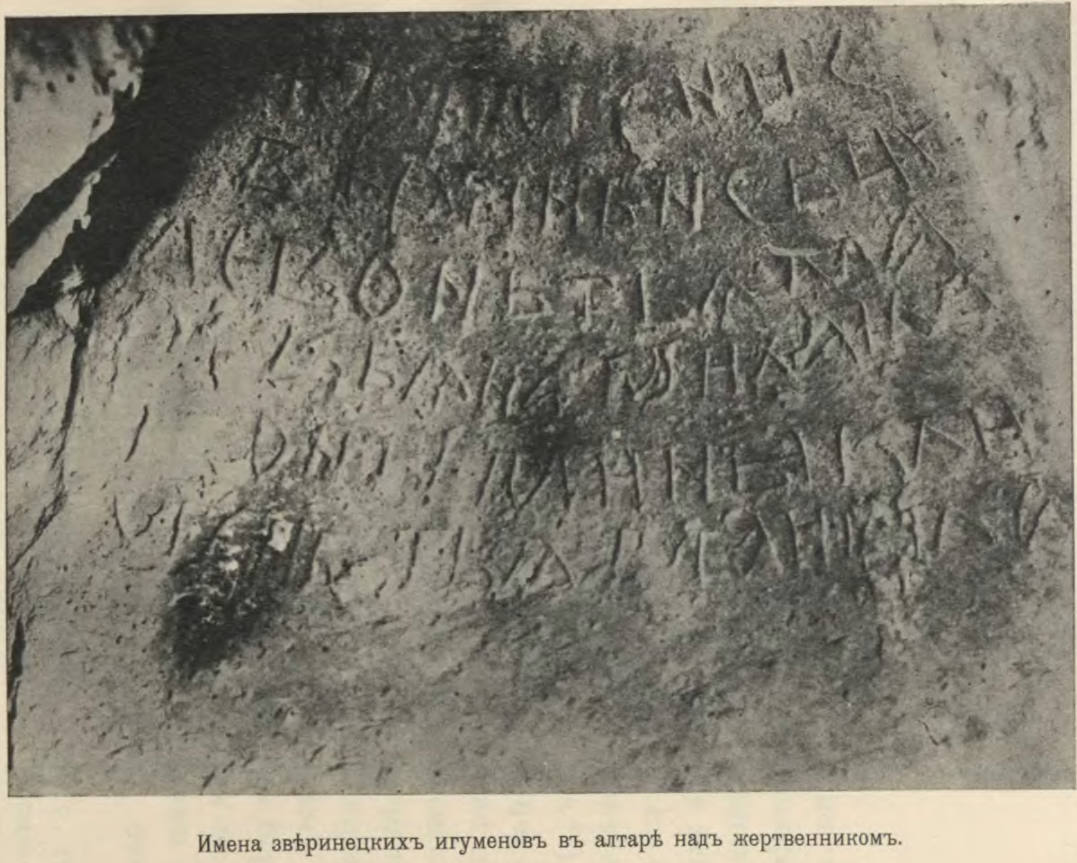
\includegraphics[width=\linewidth]{chast-colebanie-osnov/nachalo/zverp-04.jpg}
\end{center}

\vspace*{\fill}

\newpage

\begin{center}
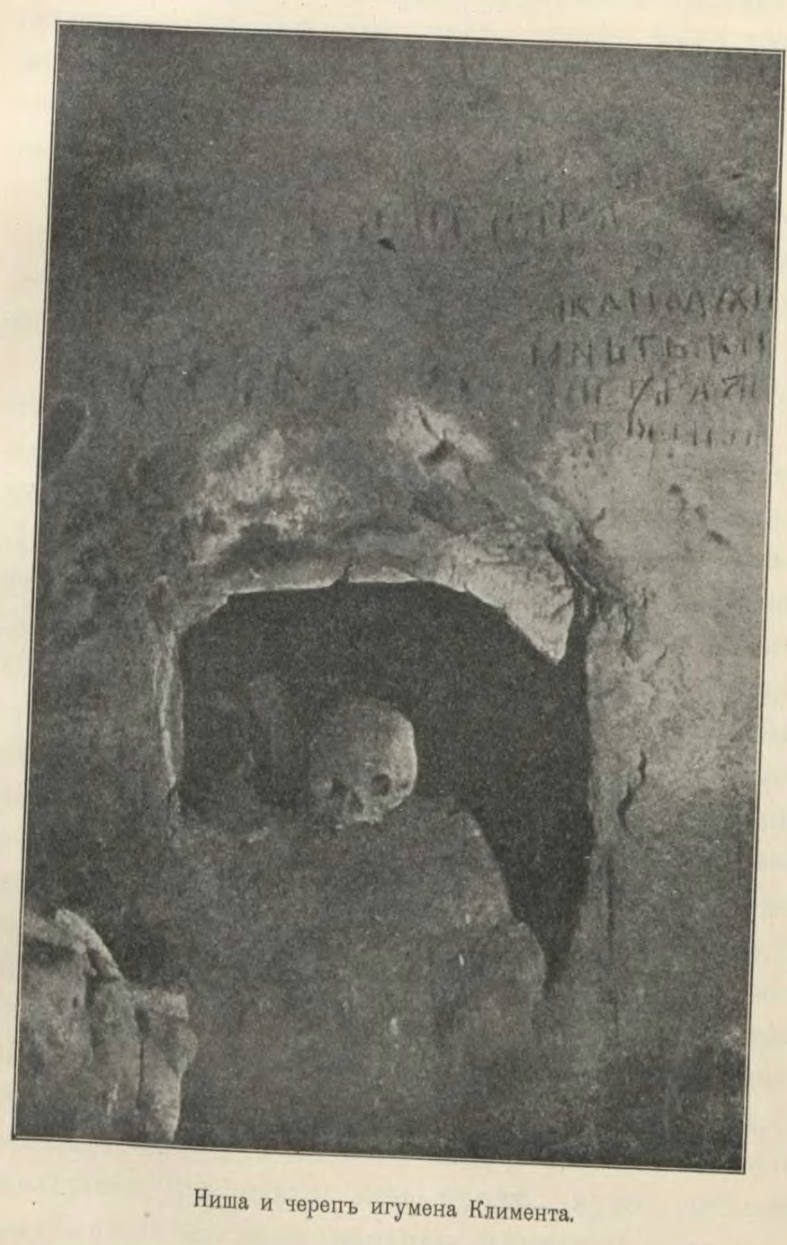
\includegraphics[width=0.95\linewidth]{chast-colebanie-osnov/nachalo/zverp-05.jpg}

\textit{Обратите внимание на соотношение глазных впадин к черепной коробке. У взрослого обычного человека черепная коробка – меньше.}
\end{center}

Что же, мы рассмотрели все надписи в пещерах. Негусто, ежели пещера использовалась людьми по крайней мере в 10, 11 и 17 веках, и если допустить, что пещера 30 лет посещалась досужими людьми, а также была наводнена зеваками в 1882 и 1888 годах.

Николай Петров задался вопросом – а так ли стары надписи на стенах?

\begin{quotation}
Некоторые из этих надписей появились, так сказать, на наших глазах, и появлялись они как бы по мере надобности в них. [...]

Далее, все подписи в новооткрытых Зверинецких пещерах начертаны одинаково, как бы рукой одного человека, – как признают это и Эртель, и г. Каманин.
\end{quotation}

Я опускаю доводы Петрова в пользу подделки надписей – желающие прочтут сами в его книжке. Не могу судить, насколько они справедливы, их нельзя однозначно ни подтвердить, ни опровергнуть. Если у нас есть выцарапанная на суглинной стене надпись, невозможно точно судить о времени ее создания, разве что по сохранности и другим надписям получится распознать, какие сделаны раньше, а какие позже.

Так что же думать? 

Все надписи были подлинно старинными, допустим 11 века? Подлинными была часть надписей, а остальные – поддельными? Все надписи, упомянутые Каманиным – подделки? Если да, то разве стены могли быть чистыми? Может, на них существовали какие-то другие граффити, а их уничтожили и написали новые, придумав для пещер историю?

А как датировать другие найденные там предметы, те же пояса?

Кожаный пояс с точно такими, как на зверинецких поясах, тиснёными иконками и надписями был в саркофаге княгини Евдокии Донской (вдовы Дмитрия Донского) в основанном ею Вознесенском монастыре московского Кремля. Княгиня была похоронена в 1407 году, но ведь могла носить пояс, уже в то время считавшийся древним.

Вот часть этого пояса – посередине изображены сцены Воскресения и Вознесения, с подписями (тоже в рамках) слева от каждой иконки:

\begin{center}
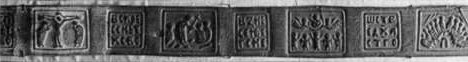
\includegraphics[width=\linewidth]{chast-colebanie-osnov/nachalo/tis02.jpg}
\end{center}

А вот часть зверинецкого – те же самые сцены:

\begin{center}
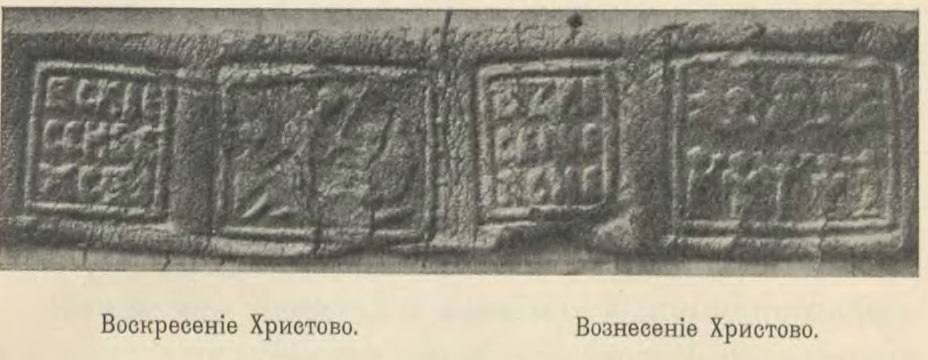
\includegraphics[width=\linewidth]{chast-colebanie-osnov/nachalo/tis01.jpg}
\end{center}

Такие же иконки (я говорю о точном подобии) тиснились на параманды – прямоугольные кожаные штуковины, носимые монахами на груди. Параманд с иконками как на «зверинецких» поясах был найден в княжеском саркофаге захоронения 14 века в 1836 году при ремонте Спасо-Преображенского на Бору собора Московского Кремля. Там же был и кожаный пояс.

Значит, по крайней мере на рубеже 14-15 веков люди носили религиозные изделия с тиснением, выполняемым одинаковым штампом. Не знаю, в разных ли местах делали эти пояса и параманды, или в одном и потом распространяли по Руси, и с какого века по какой. Определение нижней временной границы позволило бы понять, с какого времени эти пояса могли попасть в Зверинецкие пещеры.

\begin{center}
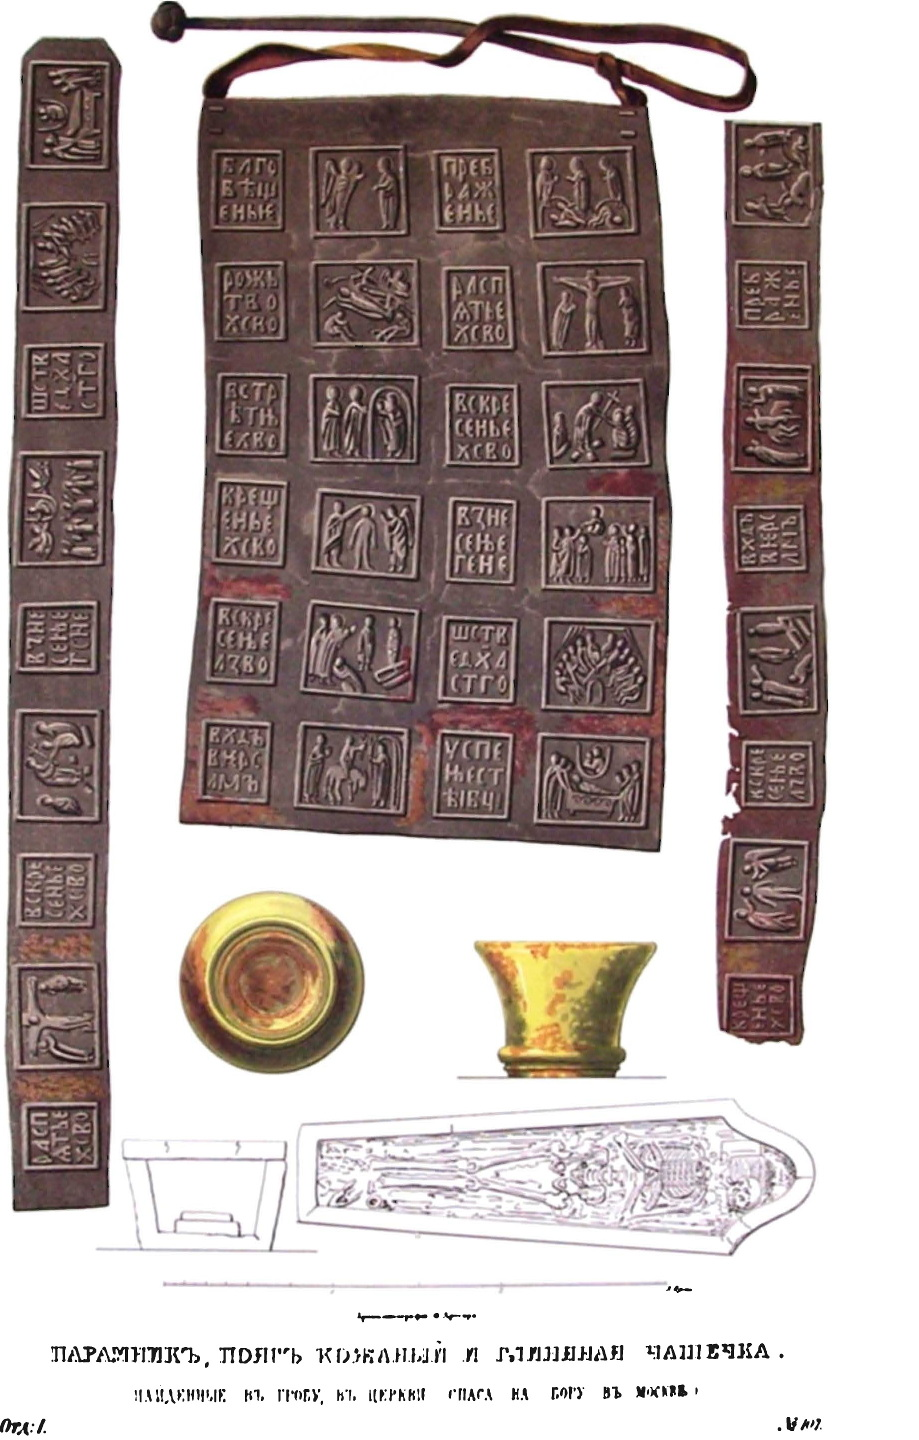
\includegraphics[width=0.94\linewidth]{chast-colebanie-osnov/nachalo/s-Drevnosti_RG_v1_ill108.jpg}
\end{center}

\textit{Из Спасо-Преображенского собора на Бору. Рисунок Фёдора Григорьевича Солнцева из книги «Древности Российскаго государства», отделение II, 1851 год.}

\newpage

%zver-pred.jpg

%Достаточно хорошо сохранились плетеные из кожаных ремешков кресты, и части поясов с выдавленными на них библейскими сценами. 

А на груди «игумена звериньского» Климентия, а точнее тела, лежащего в его поименованной нише, нашли кипарисовую (по словам Каманина) панагию – образ Богоматери с изображениями на обеих сторонах. Но панагию носили архимандриты, не игумены. Сана архимандрита вроде не было во время, к которому относят Зверинецкие пещеры.

Каманин, разбирая надпись на панагии, пришел к выводу, будто принадлежала она «Михаилу-сирину», первому киевскому митрополиту Михаилу, который, по Никоновой летописи и Степенной книге, пришел вместе с Владимиром крестить Русь и коему многие историки отказывают в существовании – мол, не было такого митрополита. Каманин же считал, что Михаил похоронен именно в Зверинецких пещерах, вероятно в «первых», открытых в 1882 году.

Николай Петров осматривал панагию и пришел к выводу, что она вовсе не кипарисовая, а оттиснута штемпелем на куске распаренного воловьего рога, и прочитал на ней первые две строчки стиха, составленного, по словам профессора, не ранее 17 века и написанные гражданским шрифтом не ранее 18 века. «Ни о каком митрополите Михаиле Сирине не может быть и речи», – заключил Петров.
\vspace*{\fill}
\begin{center}
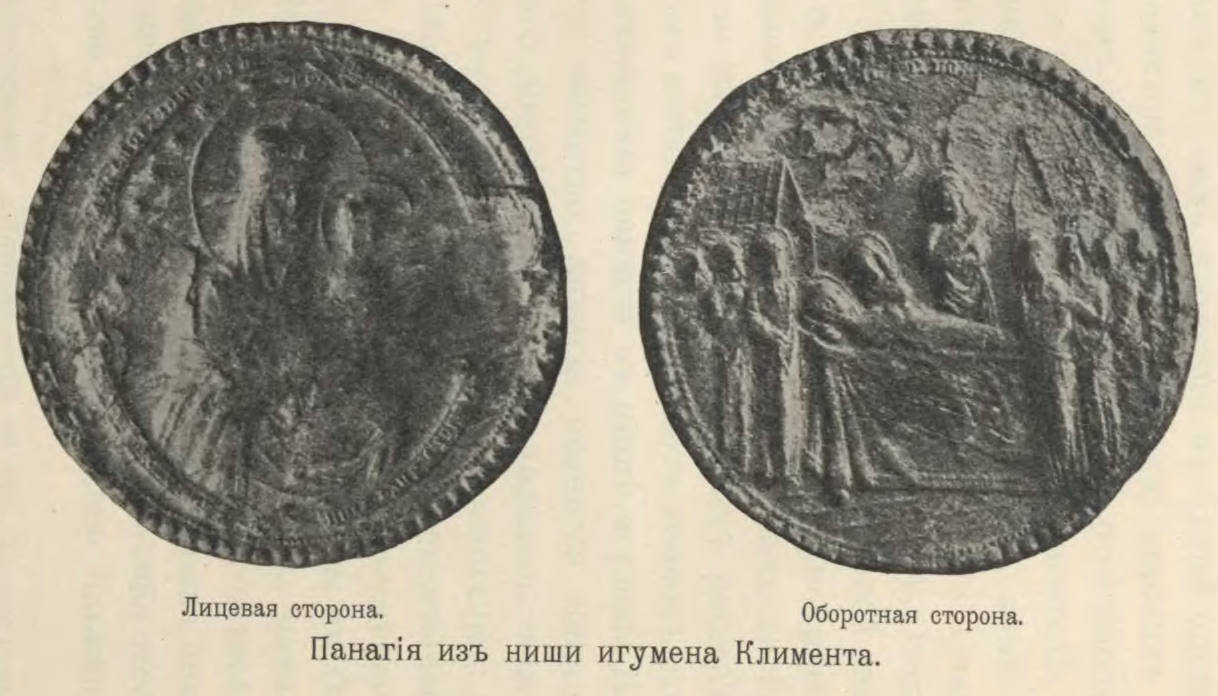
\includegraphics[width=\linewidth]{chast-colebanie-osnov/nachalo/panagia.jpg}
\end{center}
\vspace*{\fill}
\newpage

\begin{center}
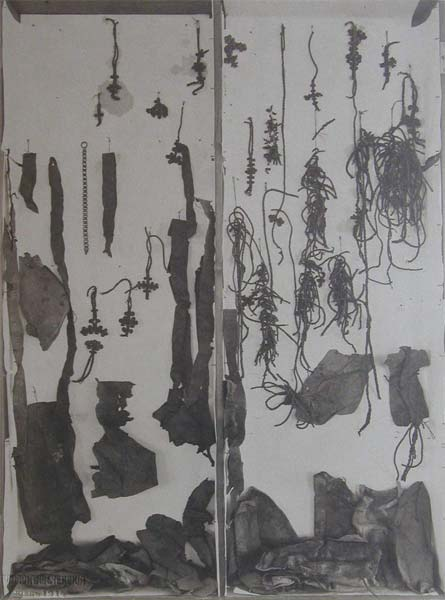
\includegraphics[width=\linewidth]{chast-colebanie-osnov/nachalo/zver-pred.jpg}
\end{center}

\textit{1914 год. Выставленные для паломников, как находки из пещер, предметы старины.}

Сомневался Петров и в древности главной находки, иконы, которую обнаружили в нише Климентия. Икона овальная, на толстой железной пластинке, покрытой эмалью, поверх которой уже писалось красками.

%У Каманина в книге, на фотографии икона выглядит иначе. 

Со времен тех дореволюционных считается, что это Одигитрия («Путеводительница») – изображение Богородицы с младенцем Христом на левой руке. Вот только нарисованное здесь далеко отлично от большинства подобных икон. Нет присущей Одигитрии сокращенной подписи «Митир Фэу Иисус Христос» («Матерь Божья Иисус Христос»). Нет нимбов. Реалистичная манера в изображении фигуры и одежды маленького. И у него странное лицо! Течение времени, повреждения краски? Да не так уж она и повреждена. Вот дореволюционный снимок:

\begin{center}
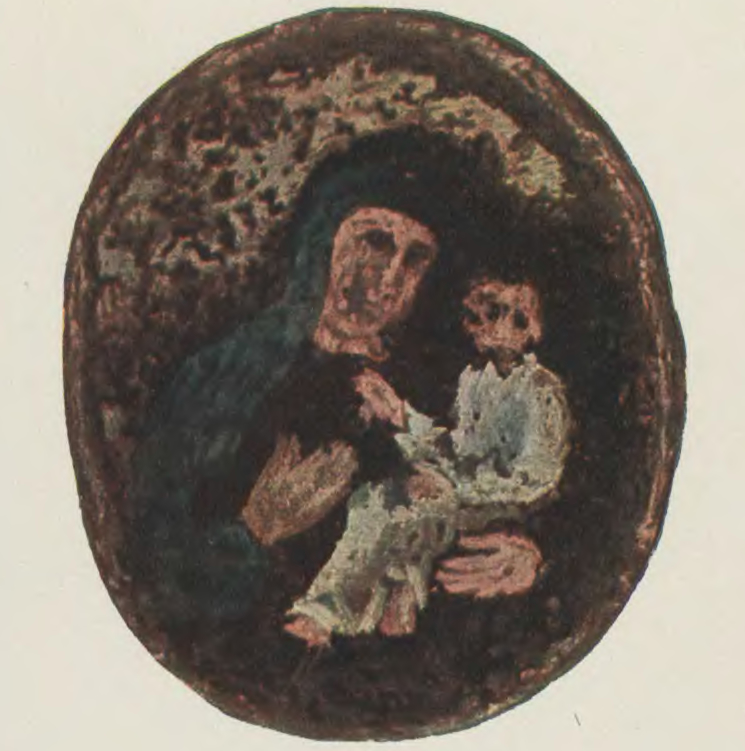
\includegraphics[width=\linewidth]{chast-colebanie-osnov/nachalo/zver-ikon.jpg}
\end{center}

Не послужит ли загадочная икона ключом к разгадке тайны Зверинецких пещер? А ведь эта икона была, коли прав Каманин, одной из древнейших славянских икон, дошедших до 20 века. Если не самой древней. 

%Нет на ней и присущей Одигитрии надписи вида: 

%\begin{center}
%\includegraphics{osn-kiev/odigitria-nadpis.png}
%\end{center}

В 1934 году, когда скит над пещерами (имевший адрес Ломаковская, 12) закрыли, икона исчезла. В разных источниках можно прочитать, что эта же икона была «чудесно обретена» в 2000-м году. Однако нашли, в 1999 году, в церкви села Селище Барышевского района, только серебряный оклад от иконы, подаренный в свое время Жеваховым.

А новую икону нарисовал в 2000 году художник А. Вовченко по дореволюционному снимку, причем с отличиями от него. Эту-то современную икону в окладе начала 20 века показывают теперь в Святотроицкой церкви Ионинского монастыря.
  
\begin{center}
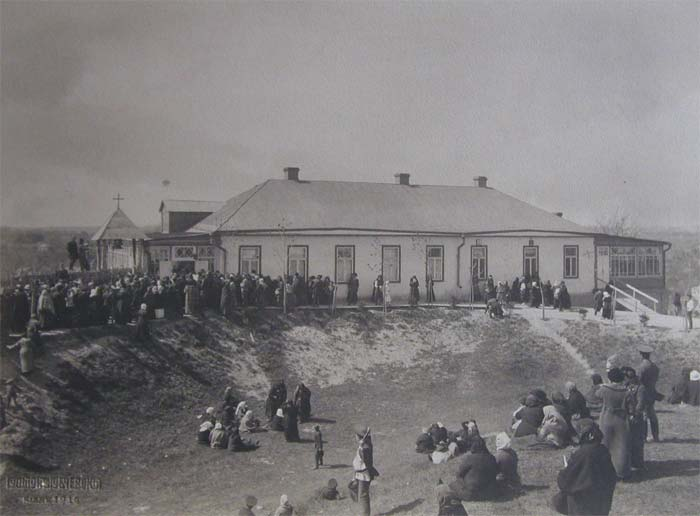
\includegraphics[width=\linewidth]{chast-colebanie-osnov/nachalo/1914-kresthod.jpg}

\textit{Окрестности Зверинецких пещер в 1914 году во время крестного хода сюда из Лавры. Возможно, фотограф стоит спиной к склону с пещерой, лицом к улице Ломаковской (Мичурина).}
\end{center}

%Пишу «Климента», а ведь надобно принять во внимание, что мы судим по найденным в пещерах надписях – а время их обнародования совпадает с раскопками Эртеля. Там был список игуменов, некоторые другие надписи, в частности две около ниши, которую сопоставили с Климентом. Надписи, по мнению Эртеля и Каманина, были древними, эдак 11 века – собственно Каманин в книге своей пытается навести мосты между летописями и списком зверинских игуменов. 

%Подвергая сомнению давность панагии и образа Богородицы, 

После открытия Зверинецких пещер 1911 года, около них создали подчиненный Лавре скит на 40 монахов и возвели церковь во имя Рождества Пресвятой Богородицы с боковым пределом, посвященным св. Иоасафу, чудотворцу Белгородскому – тому самому родичу князя Жевахова.

Предводительствовал отец Валентин (Коротенко), перешедший сюда игумен Ионинского монастыря. Валентин одолжил у Жевахова подъемные деньги, 1700 рублей и стал принимать вклады от желавших поселиться при строящейся обители. Доход приносили и паломники.

Деятельность братии и богомольцев привела к тому, что пещеры начали осыпаться. В 1913 году раскопки приостановили. Между тем продолжали впускать паломников. 

\begin{center}
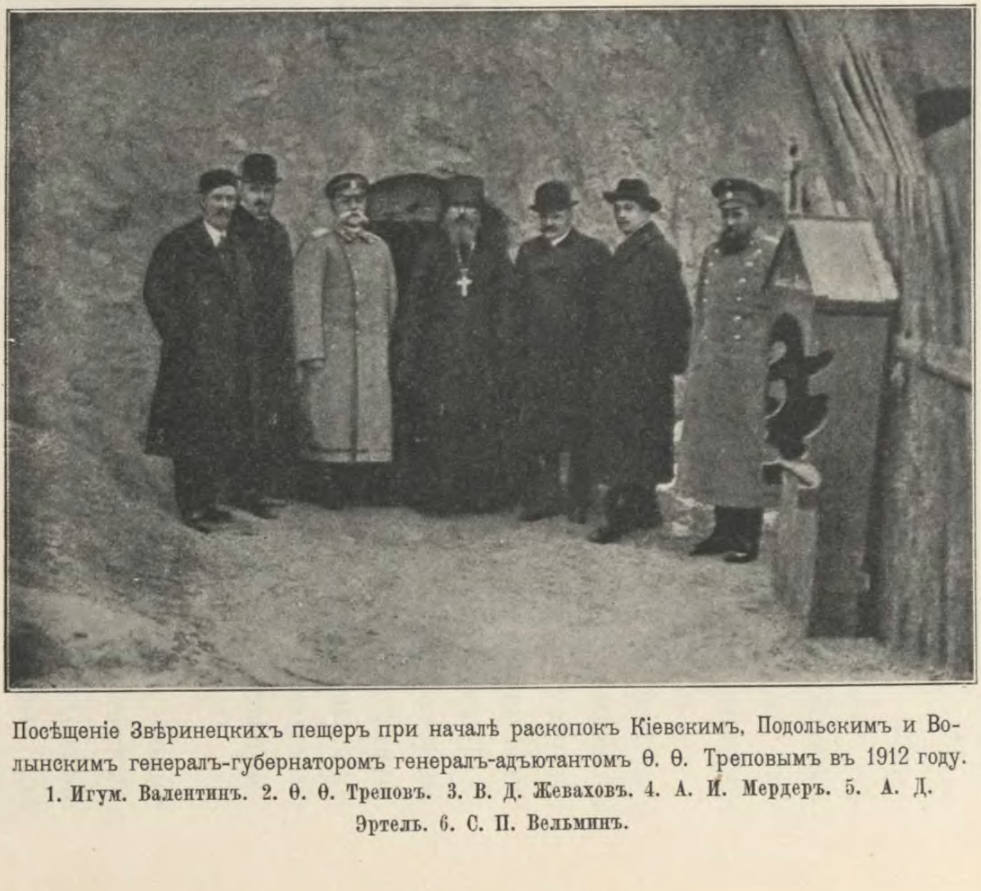
\includegraphics[width=\linewidth]{chast-colebanie-osnov/nachalo/zverp-06.jpg}
\end{center}

В 1914 году Эртель настаивал на закрытии пещер для паломников, чтобы не усугублять. И казалось бы настоял, да вышло иначе. Валентина отстранили, что, впрочем, не могло вернуть пещеры в первоначальное состояние. 

\newpage
\vspace*{\fill}
\begin{center}
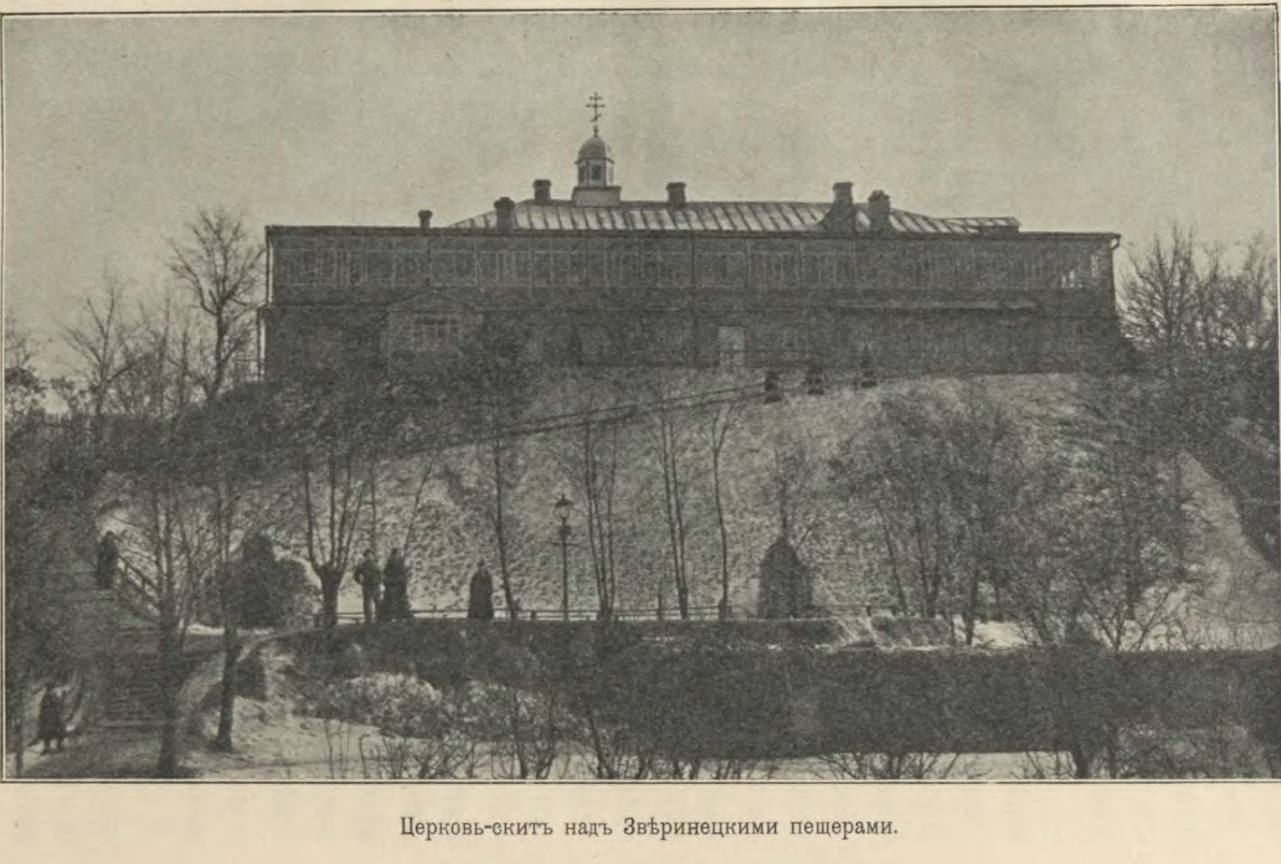
\includegraphics[width=\linewidth]{chast-colebanie-osnov/nachalo/zverp-01.jpg}
\end{center}

\begin{center}
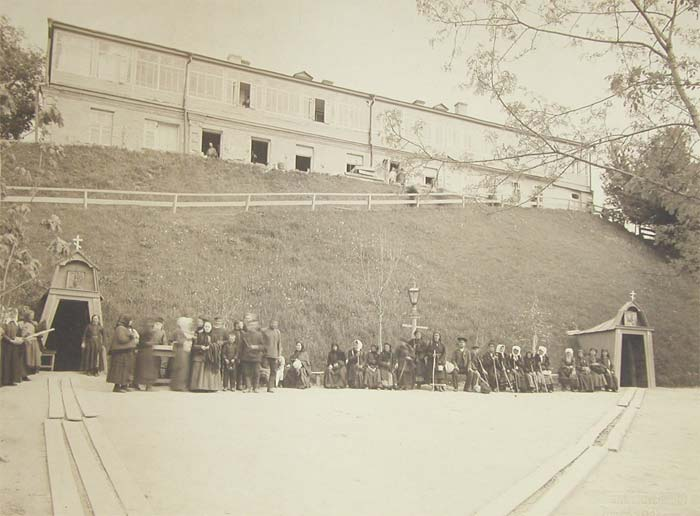
\includegraphics[width=\linewidth]{chast-colebanie-osnov/nachalo/1914-szap.jpg}

\textit{Там же, тоже вид с запада. Наверху нынче ботсад.}
\end{center}
\vspace*{\fill}
\newpage

При временном духовном безначалии – читай, при Жевахове – в 1915 году, по причине возведенного сверху подземелья храма, часть пещерных ходов укрепили оштукатуренным кирпичом, другую часть – досками. Затем скит перешел под управление иеромонаха Никанора, с которым даже Жевахов не сумел договориться о продолжении археологических работ и ремонте пещер. 

\begin{center}
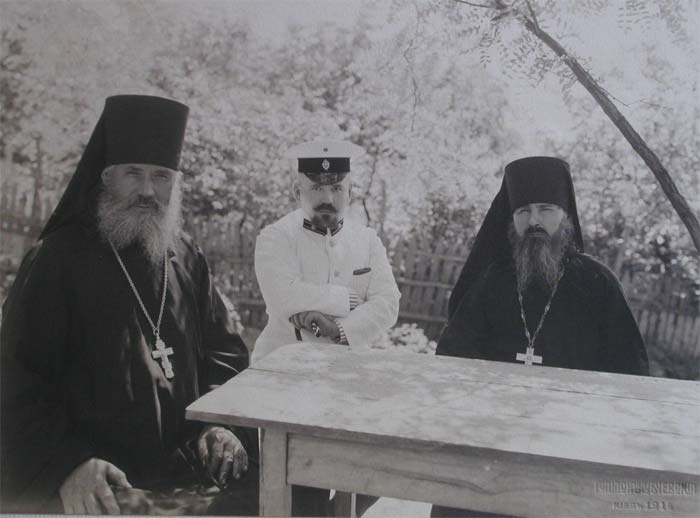
\includegraphics[width=0.90\linewidth]{chast-colebanie-osnov/nachalo/1914-nikanor.jpg}

\textit{1914. Слева направо: Никанор, Жевахов, Валентин.}
\end{center}

Разве что в 1917 году, когда очередной участок пещер стал совсем уж аварийным, Никанор разрешил позаботиться о подземельи, но с пользой для скита, дабы впридачу починили крышу надпещерной церкви. В том же году в Зверинецких пещерах похоронили отца Валентина.

Еще один удар по пещерам нанес в 1918-м\footnote{В 1918 году скит вышел из ведомства Лавры и перешел к монастырю в Церковщине (куда в марте, опасаясь большевиков, с братом Николаем скрылся Владимир Жевахов, к августу того же года впрочем ставший чиновником по особым поручениям при Министерстве внутренних дел правительства гетмана Скоропадского), а в 1925-м обрел самостоятельность.} взрыв летом пороховых складов Зверинецкой крепости, обваливший часть коридоров. Скит на поверхности тоже потерпел разрушения. Несколько позже взамен прежней церкви построили новую, в честь иконы Богоматери «Всех скорбящих радость». В окрестностях при взрыве открылись еще два пещерных хода.

В то время Киев был под немцами и гетмане Скоропадском. Его правительство сразу после взрыва объявило, что построит на разрушенном Зверинце свой центр, состоящий из Сейма, Сената, Генштаба, зданий 12 министерств.

Осенью 1918 года известному спелеологу и археологу, кстати выпускнику Киевской Духовной Академии, Игнатию Яковлевичу Стеллецкому\footnote{Большую книгу Стеллецкого «Подземный СССР» так и не издали. Впрочем опубликованы другие его работы о подземельях, среди них книга, посвященная поискам библиотеки Ивана Грозного.} поручили провести исследование подземных пустот Зверинца – выдержат ли навалившуюся власть? Стеллецкий подбирался к здешним пещерам еще в 1913 году, но Эртель не захотел тогда сотрудничать. И вот в январе 1919 года Стеллецкий приступил к работе. В марте привлек к раскопке и Эртеля, которого год назад завалило под землей на Ломаковской, с повреждением таза, руки и переломом ноги. Кажется, Стеллецкого больше заботила не застройка Зверинца, а сами пещеры. Он писал:

\begin{quotation}
В археологическом отношении встала передо мной тяжелая, значительная и в полной мере интересная задача – доказать, что открытые уже пещеры на Зверинце есть только продолжение катакомб старинного пещерного Выдубицкого монастыря непосредственно соединенного подземными нитками – соединениями с современным наземным Выдубицким в такой же мере, как так называемые Ближние или Дальние пещеры с Печерской Лаврой.
\end{quotation}

Также, Стеллецкий считал, что все эти пещеры были вырыты еще в неолит, а монахи лишь приспособили их под свои нужды.

Дневники раскопок и статьи Стеллецкого хранятся в Российском государственном архиве литературы и искусства, 208 листов, посмотреть их у меня нет возможности. Сведения о них черпаю только из сторонних, зачастую отрывочных источников.

%Стеллецкий взялся исследовать один из возникших после взрыва провалов, что вёл в древнюю пещеру с шаровидной комнаткой, где было «детское погребение» и лежали плиты сланца, древние плоские кирпичи – плинфы, еще какие-то предметы будто великокняжеских времен. Наверх от комнатки, в сторону Зверинецких пещер шел коридор с боковыми нишами, в коих тоже были захоронения. Получается, этот провал был ниже по склону, чем Зверинецкие пещеры 1911 года.

%Другой провал, около Экономических ворот Троицкого монастыря\footnote{Я не знаю, где они находились. Экономические ворота в монастыре обычно ведут к экономическому двору, и приспособлены для проезда через них с возами. О прошлом монастыря приходится судить лишь по фотографиям, ибо документация его сгорела при памятном взрыве Зверинецкой крепости.}, явил подземелье со стенами, обшитыми истлевшими досками. Его расчистили на 21 метр. Вход туда был размыт водой. Назначение сего помещения не определили. Ни среди обычных монашеских пещер, ни крепостных подземных коридоров – потерн, с таким не сталкивались.

Вот в заметке «К истории раскопок пещер
на Зверинце в Киеве (по поводу застройки Зверинца)» Стеллецкий писал (примечания по ходу мои):

\begin{quotation}
А раз так, то окончательно загадочным является подземелье, обнаруженное котлованом возле
Экономических ворот Троицкого монастыря\footnote{Я не знаю, где они находились. Экономические ворота в монастыре обычно ведут к экономическому двору, и приспособлены для проезда через них с возами. О прошлом монастыря приходится судить лишь по фотографиям, ибо документация его сгорела при памятном взрыве Зверинецкой крепости.}.
Раскопки его дают пока такую картину.

Провал образовался в своде какого-то высокого\footnote{Какова же высота?} подземного помещения, может быть, имевшего здесь входной люк. На глубине 12–13 арш\footnote{8,53-9,26 м.}.
обозначился широкий, до 3 арш.\footnote{2,1 м.}, коридор, направлением к югу, суживающийся к полу, подобно зверинецкой пещерной церкви и расширяющийся в боках. 

Самый коридор постепенно суживается вперед и опускается вглубь. Затянут он плотно илом от стремительно затекавшей сюда воды, срывавшей разной величины доски\footnote{Обшитый досками подземный ход Стеллецкий раскапывал и за 5-й гимназией, это сейчас Суворова, 1.} и бревна, которыми был обшит ход, то и дело попадающихся в разных слоях и на разной высоте намула.

Собственно над полом нанос не добирается
вершка на два, с целью не натаптывать, а доследовать пол особо. Свод коробовый, обработан небрежно и грубо.

Может быть, в дальнейшем ход примет нормальную ширину, но пока в этом отношении он выходит из рамок всего, что мне до сих пор приходилось встречать.

А. Д. Эртель склоняется к мысли, что это -
«паттерна» – стратегический ход. Я лично этого не думаю, так как считаю, что он для этого без нужды глубокий.

Я наблюдал в Пернове кавалерийский подземный ход: он, высокий, обложенный камнем, шел сквозь вал и, не выходя из последнего, поворачивал под прямым углом вправо, шел несколько вдоль вала и затем выходил в овраг с противоположной стороны.

Образчик стратегического пехотного хода
представляет выложенный местным камнем ход вокруг крепостной стены в Пскове. Внутри этого хода характерны слухи – углубления в своде, через которые слышен наружный разговор. Само собою разумеется, что и самый ход для этого был заложен не глубоко от поверхности, всего на 1 сажень. Типичные же образчики собственно «паттерн» имеем в укреплениях на Лысой Горе, где «паттерны» проходят в валах, почти не углубляясь в материк.

Зверинецкий новооткрытый ход как нельзя
более далек от этих образчиков стратегических ходов. Он есть какая-то новая разновидность в категории таинственных подземных памятников и потому вдвойне интересным представляется его дальнейшее исследование.

Другой котлован, на противоположном конце
«Укрепления»\footnote{Как понимаю, речь идет о Зверинецкой крепости и той ее части, что от современного Розария протянулась к перекрестку, где спуск в Сиреневую аллею и дорога к Ионинской церкви. Возможно, где-то в окрестностях этой точки – 50°25'02.6"N 30°33'41.2"E.}, близ разрушенной церкви скита, на глубине около 13–14 арш. дал погребение младенца с инвентарем X–XII вв.\footnote{В другом источнике упомянута – пещера с шаровидной комнаткой, где было «детское погребение» и лежали плиты сланца, древние плоские кирпичи – плинфы, еще какие-то предметы будто великокняжеских времен.}, а вслед затем, в с.с. углу стены найдены были признаки обрушившейся пустоты, другими словами, опадающий глыбами свод какого-то подземелья.

Прокопаться в это подземелье будет легче первого, потому что оно совершенно сухое и не затянуто илом; пустота должна открыться немедленно.

Открыто на днях и еще одно подземелье,
вернее, целый лабиринт, пока, однако, не исследованный – в Троицком монастыре.
В свое время оно раскапывалось любителем-иноком, но потом засыпанная часть коридора была заложена кирпичом, а вычищенная обращена под монастырский погреб\footnote{Не о пещере ли под склоном с колокольней идет речь? Так значит, там был целый лабиринт?}.

Наконец, в Выдубицком монастыре, на подворье, соединяющем Выдубицкий монастырь через Троицкий со Зверинецким акрополем, старик-монах, правда безуспешно, пытался показать место хода, который он наблюдал здесь лет 40 тому назад.

Эти данные еще более утверждают меня в
мысли, что Выдубицкий монастырь связан подземными артериями со Зверинецкими катакомбами. 

Киев. 1919.IV.12. Игн. Стеллецкий
\end{quotation}

Стеллецкий собирался продолжать археологические работы. Застройка Зверинца тормозилась, а потом власть переменилась и вопрос отпал. Чем завершились исследования Стеллецкого, я не осведомлен.

Скит на Зверинце продолжал существовать и паломники посещали пещеры. В 1924 году Жевахов принял в скитской церкви монашество как Иоасаф, два года жил в близлежащем Ионинском монастыре, а в 1926 перебрался в Зверинецкий скит и получил сан епископа. Последующие 11 лет, с перерывами – лагерь, ссылка, тюрьма – и так до расстрельного приговора тройки при УНКВД по Курской обл. 04/12/1937 по обвинению в «руководстве контрреволюционной фашистской организацией церковников». Приговор был исполнен в тот же день.

В 1934 году скит закрыли, постройки со временем разобрали. В 1980-х я нашел на его месте дореволюционный кирпич, кажется с клеймом «Х.ВОЛКОВЪ».

В 1965-м в Зверинецких пещерах провели археологическую разведку, о которой я знаю только, что исследователи установили, будто во время фашистской оккупации в пещерах прятались люди. В том же 65-м исторический памятник получил охранный паспорт\footnote{
\begin{quotation}
Взято під охорону згідно постанови Ради Міністрів УРСР № 711 від 21.07.1965 р.

Охоронний №: 139

Межі охоронної зони і зони регулювання забудови: згідно рішення виконкому Київської міської Ради народних депутатів № 920 (додаток І, п. 1, 2, 3) Звіринецькі печери входять в зону археологічного заповідника (р-н Видубицького монастиря та Звіринецькі печери). 
\end{quotation}

В указанном постановлении 711 в разделе III «ПАМ'ЯТНИКИ АРХЕОЛОГІЇ», под номером 
139 указаны «Звіриницькі печери, Печерський район, Звіринець» – с примечанием «з настінними написами (XI-XIII ст. ст.)». Постановление было отменено 03 сентября «Постановой КМ № 928 (928-2009-п)», и тогда же пещеры занесли в новый реестр, Государственных недвижимых памятников Украины, как объект культурного наследия под номером 260034-Н – археологический памятник 11-17 веков, по адресу Мичурина 18-22.}, переоформленный в 2009 уже для нового реестра.

В 1979 году пещеры посетили археологи из Киевской лаборатории спелеологических исследований. Тогда-то, надо полагать, и передвинули будку нужника в сторону от входа в подземелье.

На сегодня определены – их приводят в книгах\footnote{Например, «Историко-градостроительные исследования Киева» под редакцией В. Вечерского, Киев, Феникс, 2012.} – границы зоны охраны культурного слоя первой категории вокруг памятника «Зверинецкие пещеры»:

%На сегодня определены границы зоны охраны культурного слоя первой категории вокруг памятника «Зверинецкие пещеры»:

\begin{quotation}
от пересечения ул. Мичурина и переулка Мичурина по правой стороне улицы Мичурина в юго-восточном направлении (до усадьбы № 28), оттуда в юго-восточном, юго-западном и северо-западном направлениях (территория Центрального ботанического сада им. М. Гришко НАН Украины) до пересечения с ул. Мичурина.
\end{quotation}

Попытайтесь наложить это описание на карту, и у вас ничего не получится, поскольку от пересечения улицы Мичурина с переулком можно двигаться по правой стороне только на северо-восток, а не на юго-восток.

В конце 20 столетия паломничество в пещеры возродилось, Музей Киева провел реставрационные работы, одновременно добиваясь отселения жителей из усадеб на Мичурина с номера 18 по 24, на четной, подгорной стороне.

В начале 21 века в усадьбе с пещерами, при созданном монастыре, возвели собор, а окрестности постигла тяжелая перестройка. На месте скромных стареньких домиков, белеющих через листву садов, огороженных кривыми заборами, вдруг возникли терема за крепостными стенами, коих устрашился бы сам Батый.

Летом 2017 года мы с Дашей Кононюк посетили Зверинецкие пещеры, побывали там впервые. За толстой, обложенной камнем стеной усадьбы – церковные здания, соединенные друг с другом и покрывающие склон. Двери, лестницы. Всё построено добротно и основательно. В церковной лавке мы разговорились со служителем церкви, который познакомил нас со священником. Тот любезно проводил нас в пещеру и рассказал много полезного. Если о нераскопанном ходе в сторону Ионинской церкви мы знали, то сведения про нераскопанный же ход в направлении Выдубицкого монастыря был новостью.

Дойдя с нами до половины пещеры, священник оставил нас одних и мы продолжили осмотр. Несмотря на жару снаружи, внизу было столь холодно, что изо рта шел пар.

Пещера основательно укреплена, местами оштукатурена. Высота потолков в коридорах, кроме одного места, более чем достаточна для прохождения посетителей, еще с запасом. Освещения не было, кроме взятого с собой – священник и Даша держали в руках свечи, а я фонарик.

Пустые комнатки (я избегаю слова келья, указывающее на место жительства монаха) по обеим сторонам коридоров ничем не защищены, а вот наполненные костями закрыты черными коваными решетками. Некоторые имеют длину явно меньшую, чтобы там лежа мог поместиться взрослый человек обычного роста. Даже если это чисто погребальные ниши, то для тела детского или подросткового роста.

Среди комнаток были такие, где можно находиться сидя. В одной по бокам было два «лежака», а между ними выемка.

Современные Зверинецкие пещеры я могу назвать, скорее, пещерами созданными недавно на основе древних пещер, поскольку от седой старины в нетронутом виде не осталось ничего. Да и сама окружающая местность преобразилась.

\vspace*{\fill}

\begin{center}
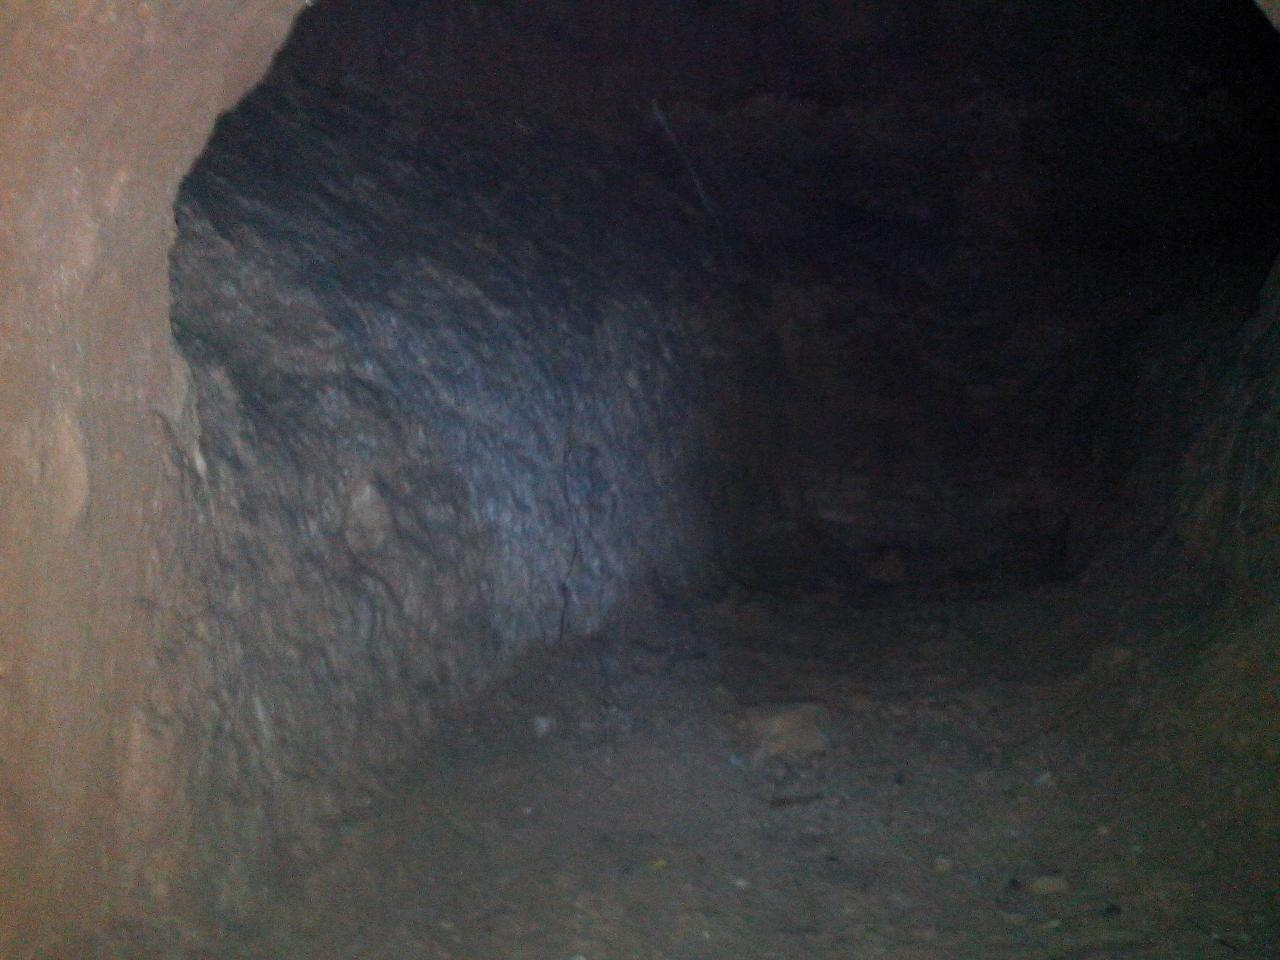
\includegraphics[width=0.98\linewidth]{chast-colebanie-osnov/nachalo/IMG_20170626_135030.jpg}

\textit{Комнатка с лежаками.}
\end{center}

\vspace*{\fill}


\newpage

\begin{center}
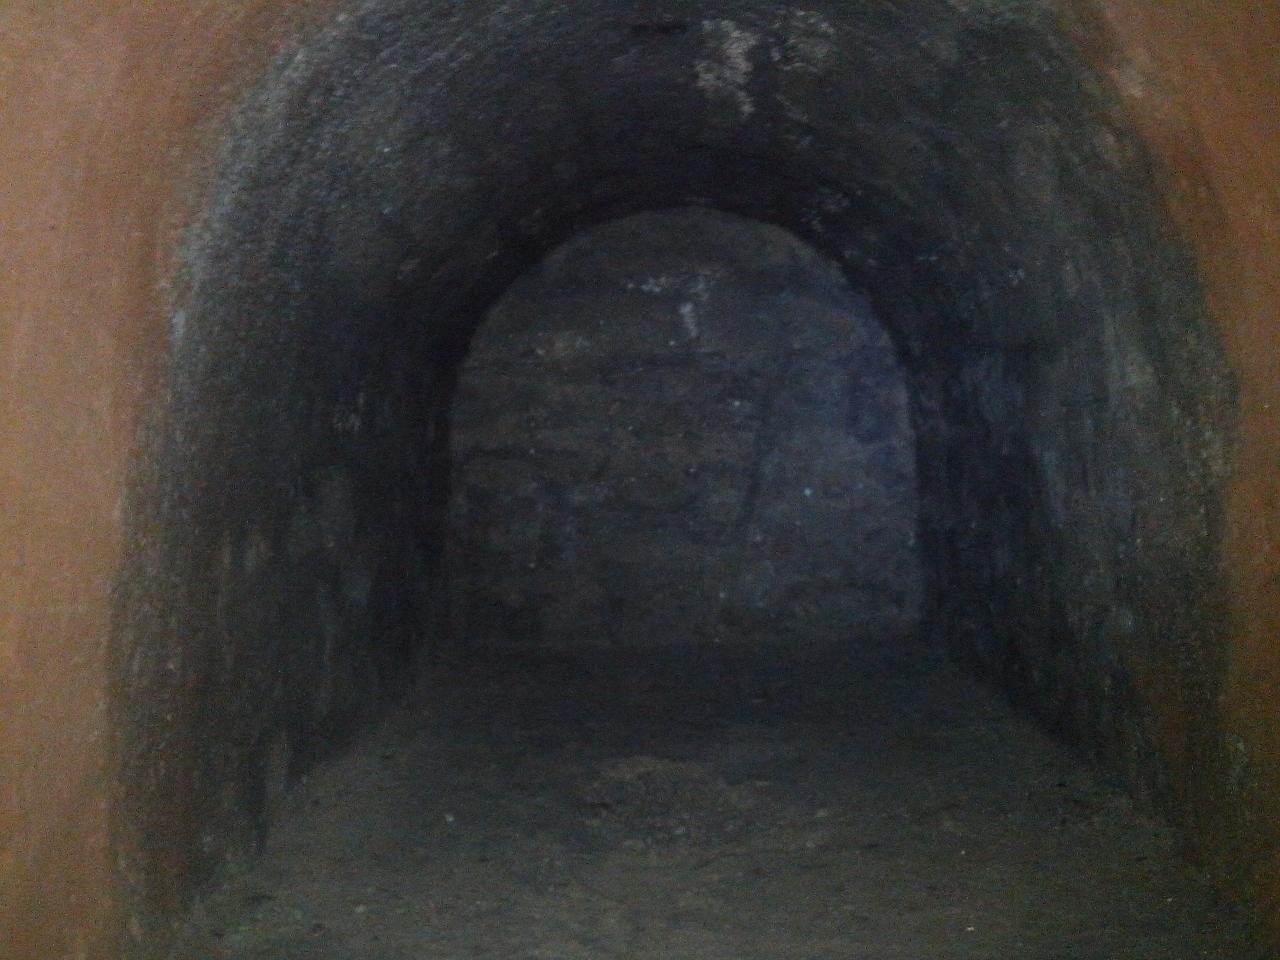
\includegraphics[width=0.98\linewidth]{chast-colebanie-osnov/nachalo/IMG_20170626_135106.jpg}

\textit{Одна из многочисленных «погребальных ниш» малой длины.}
\end{center}

\begin{center}
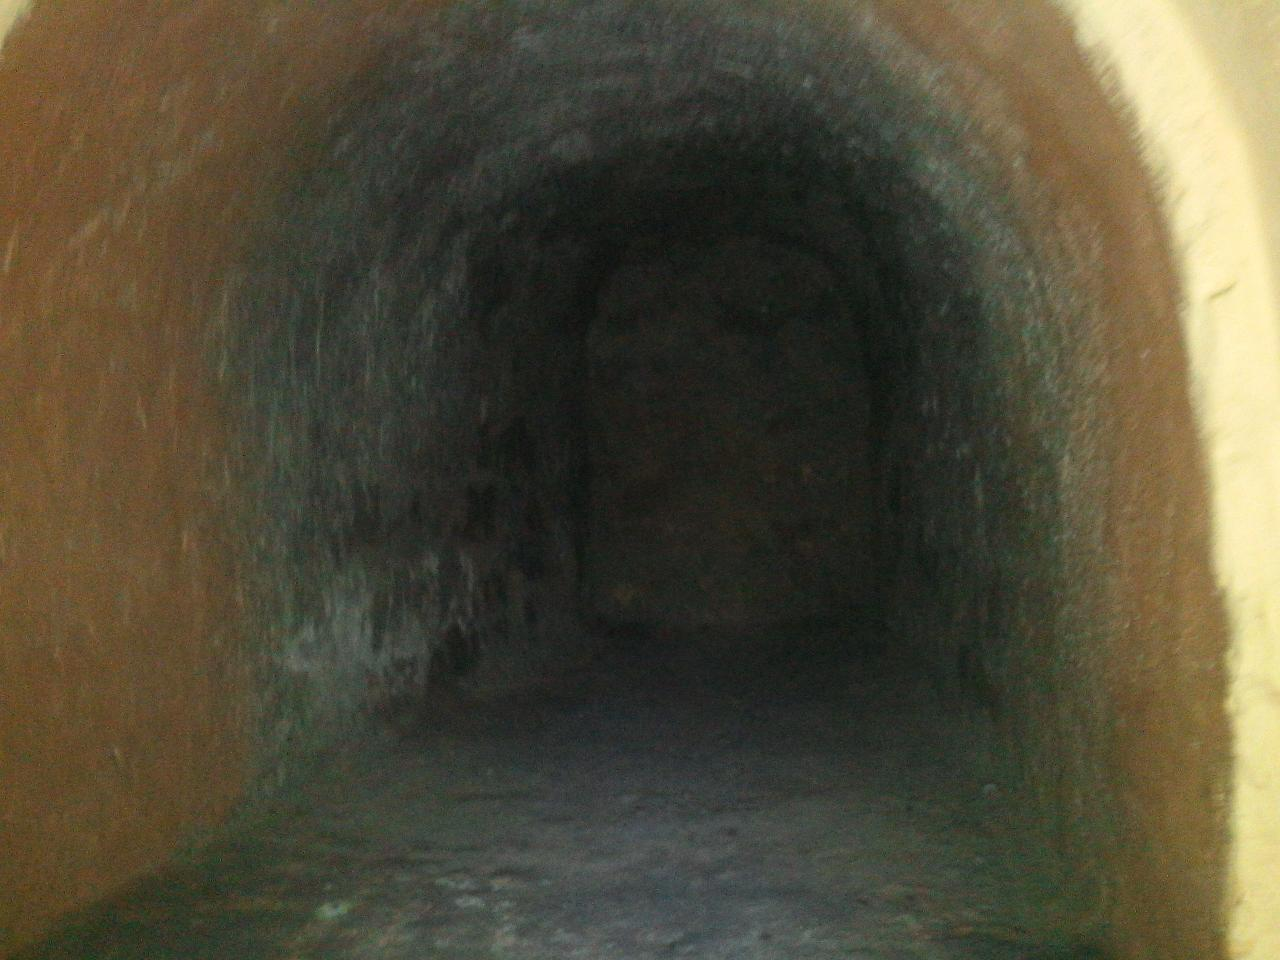
\includegraphics[width=0.96\linewidth]{chast-colebanie-osnov/nachalo/IMG_20170626_135152.jpg}

\textit{Еще одна.}
\end{center}

\newpage
\vspace*{\fill}
\begin{center}
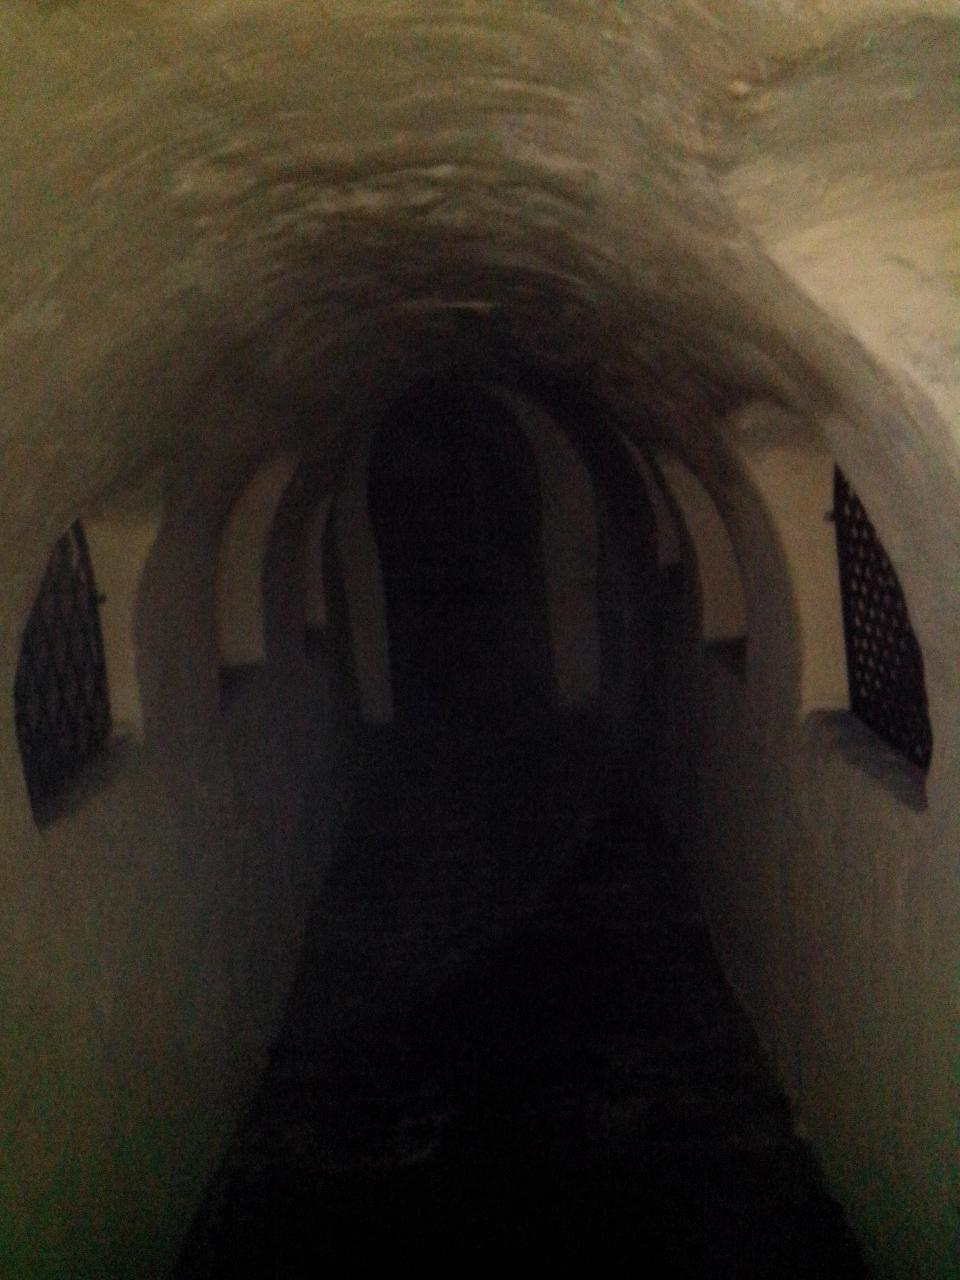
\includegraphics[width=\linewidth]{chast-colebanie-osnov/nachalo/IMG_20170626_135248.jpg}

\textit{Коридор с «погребальными нишами».}
\end{center}
\vspace*{\fill}

\newpage

\vspace*{\fill}
\begin{center}
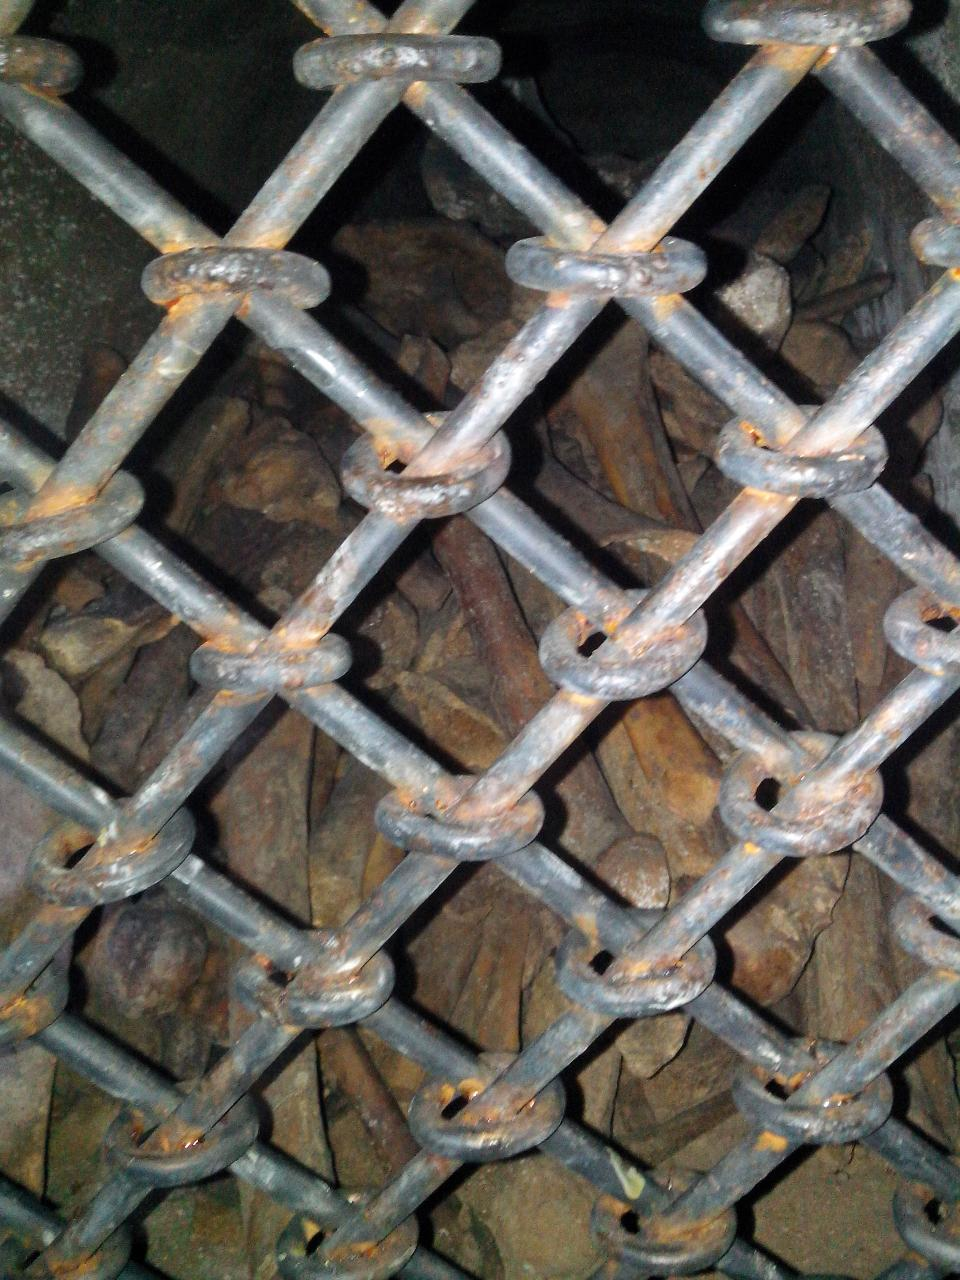
\includegraphics[width=\linewidth]{chast-colebanie-osnov/nachalo/IMG_20170626_135243.jpg}

\textit{Прах к праху. Чьи вы руки и ноги, как выглядели целыми во плоти?}
\end{center}
\vspace*{\fill}
\newpage
\vspace*{\fill}
\begin{center}
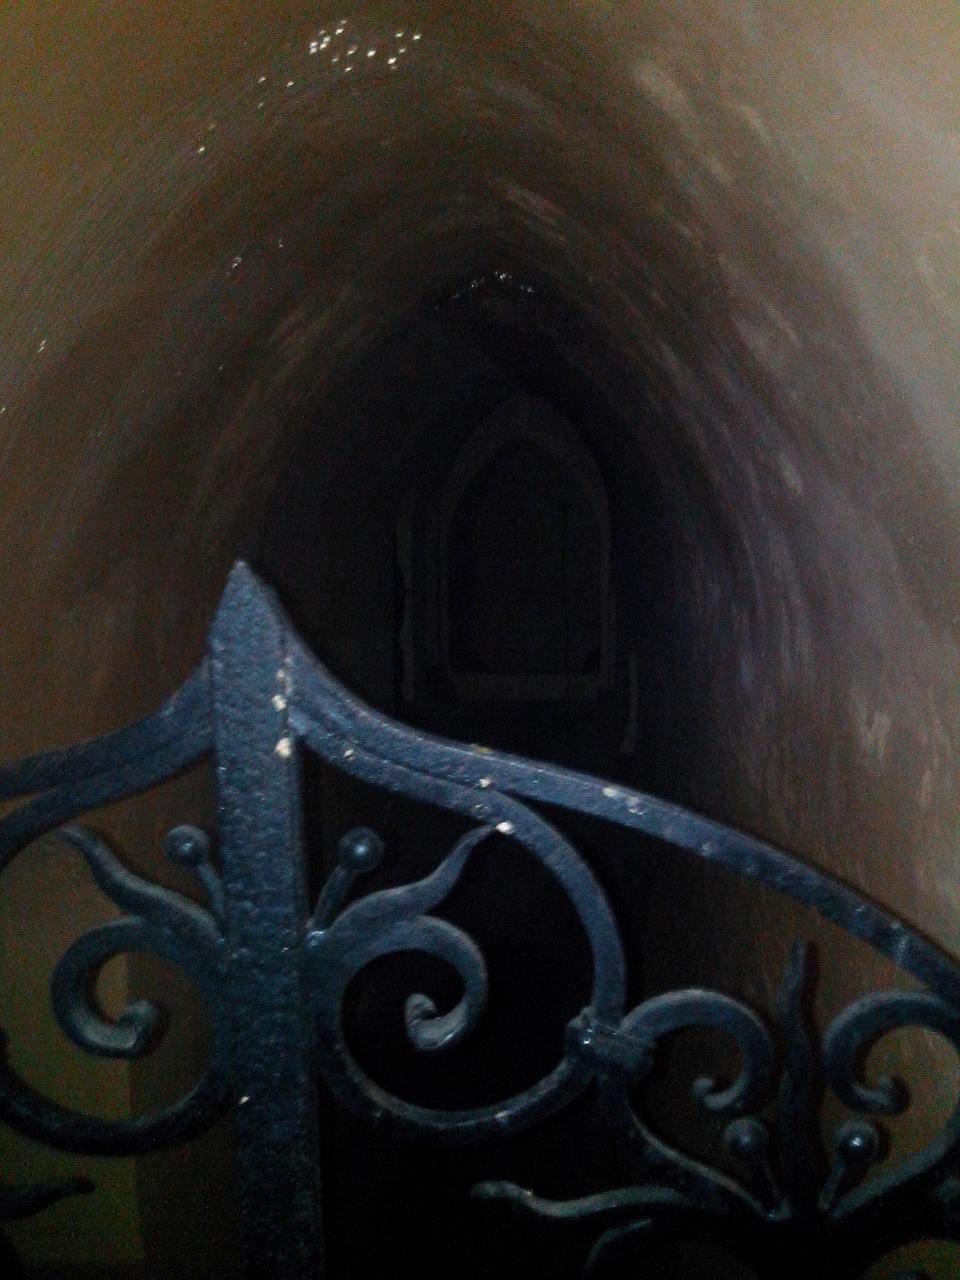
\includegraphics[width=\linewidth]{chast-colebanie-osnov/nachalo/IMG_20170626_135548.jpg}

\textit{Коридор ведет к нераскопанной части пещер. Что там дальше?}
\end{center}
\vspace*{\fill}
\newpage

Но я помню тот еще прежний, в зелени садов поворот на Мичурина, под пещерами, с домом некой бабы Даши напротив – у нее козы жили, а хатка пряталась за кустами сирени. Про пещеры я знал тогда очень смутно, мне они были до лампочки. А ведь ходил мимо почти каждый день.

Я мало увлекался этим всем, живя около ботсада и окруженный древностью со всех сторон. Не говорю об Ионинской церкви, это сравнительный новодел, а во время моего детства она была еще просто государственным зданием, там вечно происходила реставрация, я заходил внутрь, кроме строительных лесов было пусто, а вне стен, на траве валялись куски мозаики – я подобрал несколько больших кусков и хранил дома. Напротив церкви, двухэтажная старенькая колокольня с круглыми часами, на всю округу отбивала каждый час. Я слышал ее даже дома.

Ботанический сад имени Гришко расположился на буквально летописных холмах Зверинца. В глубокой ложбине спрятался монастырь Выдубичи, с его заметными куполами – на колокольне синий в звездах, а другие зеленые. На одном из окрестных склонов в седую старину был Всеволож Красный двор. Вроде бы именно его остатки нашли советские археологи в семидесятых годах на соседствующем с Выдубами, к северу, углу горы – хотя понятно, что никакой таблички с названием при раскопках не обнаружили.% Как по мне, князю выгоднее было строиться там, где в ботсаду перекресток у верха сиреневой аллеи, хвойных и дороги к Ионинской церкви.

Сейчас Красный двор, что называется, возродили – поставили на холме (в 700 метрах от Зверинецких пещер), известном как мыс Чайка,  ограду из бревен, бревенчатую же башню о двух этажах\footnote{50.421302634400284, 30.56695182662565}, и памятный камень с фамилиями тех, кто сему способствовал. В той же местности находилась гончарная слобода, эдак в столетии 13-14. Археологи нашли полные готовой посуды печи, а что случилось, почему всё бросили, неясно.

Напротив основной Зверинецкой горы, к северу – другая гора, со Зверинецким кладбищем, а за нею в удольи – Наводницкий ручей. Он бежит в коллекторе, однако до 2014 года в пойменном овраге сохранялось и поверхностное его течение, питаемое сочащимися со склона кладбища родниками. Затем на уцелевшем отрезке ручья развернули строительство и всё пропало. 

%Прежде там, на перекрестке бульвара Дружбы Народов и улицы Старонаводницкой, у подножия трех холмов – Зверинецкого, кладбищенского и с Родиной-матерью – была конечная остановка троллейбуса. 

%А еще ранее там же Неводницкий ручей, купно со стоком лежащего к юго-западу озеру Святому (о нем читайте в отдельной главе про Зверинец) образовывал озеро Проклятое, соединяющееся с Днепром. 

В восьмидесятые годы прямо рядом с кладбищем, на Верхней улице возвели больницу Четвертого управления. А вместо близлежащей высотки по третьему номеру, был частный сектор – пал жертвой строительства. Маленьким, однажды я бродил там в саду около развалин и нашел игрушки: фиолетовую уточку на колесиках, со ржавой осью, да печального резинового пёсика с пищалкой. Хорошо это запомнил, ибо тогда я впервые увидел разрушенный, снесенный дом.

Западный из южных отрогов Зверинца называется Бусовой горой, а напротив нее, через железную дорогу и летописную речку Лыбедь – Лысая, она же Девич-гора, с остатками крепости. У низовья ботсада, перед железной дорогой, возле ручья под склоном, мы с мамой опять-таки в начале восьмидесятых нашли доисторическую штуку из гладкого камня. До сих пор не знаю, что это. 

Тогда в Выдубицком монастыре помещался Институт археологии. Мы понесли штуку туда – «показать специалистам». Специалистам она оказалась пофиг, и с тех пор занимает дома почетное место на книжной полке рядом с окаменевшей ракушкой.

Смутно помню, как зашли мы в один из корпусов института, бывшее монастырское здание. Потолки высокие, стены толстые. Тихо, темновато, прохладно. Обратились к тетеньке-ученой. Она покрутила предмет в руках. Еще голову так наклоняла, сбоку набок. Потом скучно сказала, что это наверное дети баловались и вылепили из глины. Ученым такое не нужно. С тем мы и ушли.

%Уже в 2013 году я обратился за помощью с определением штуковины к археологам, в одно из сетевых сообществ. Без толку. 

Но штуковина – из кремня, а не глины. Орудия труда «каменного века» обычно лишены такой шлифовки. Поверхность нашей находки гладкая, камень удобно лежит в руке и будто, в самом деле, под нее вылеплен. А с одного конца есть ровная каёмка. Быть может, в этом месте предмет к чему-то крепился и, вращаясь (что и послужило шлифовке) был частью некоего приспособления?

%В 2013 году я наступил на грабли, попросив археологов о помощи в определении. Пошла потеха! Что же, плачевно состояние той науки, чьей представителям насмешка служит средством к познанию.

\newpage
\vspace*{\fill}
\begin{center}
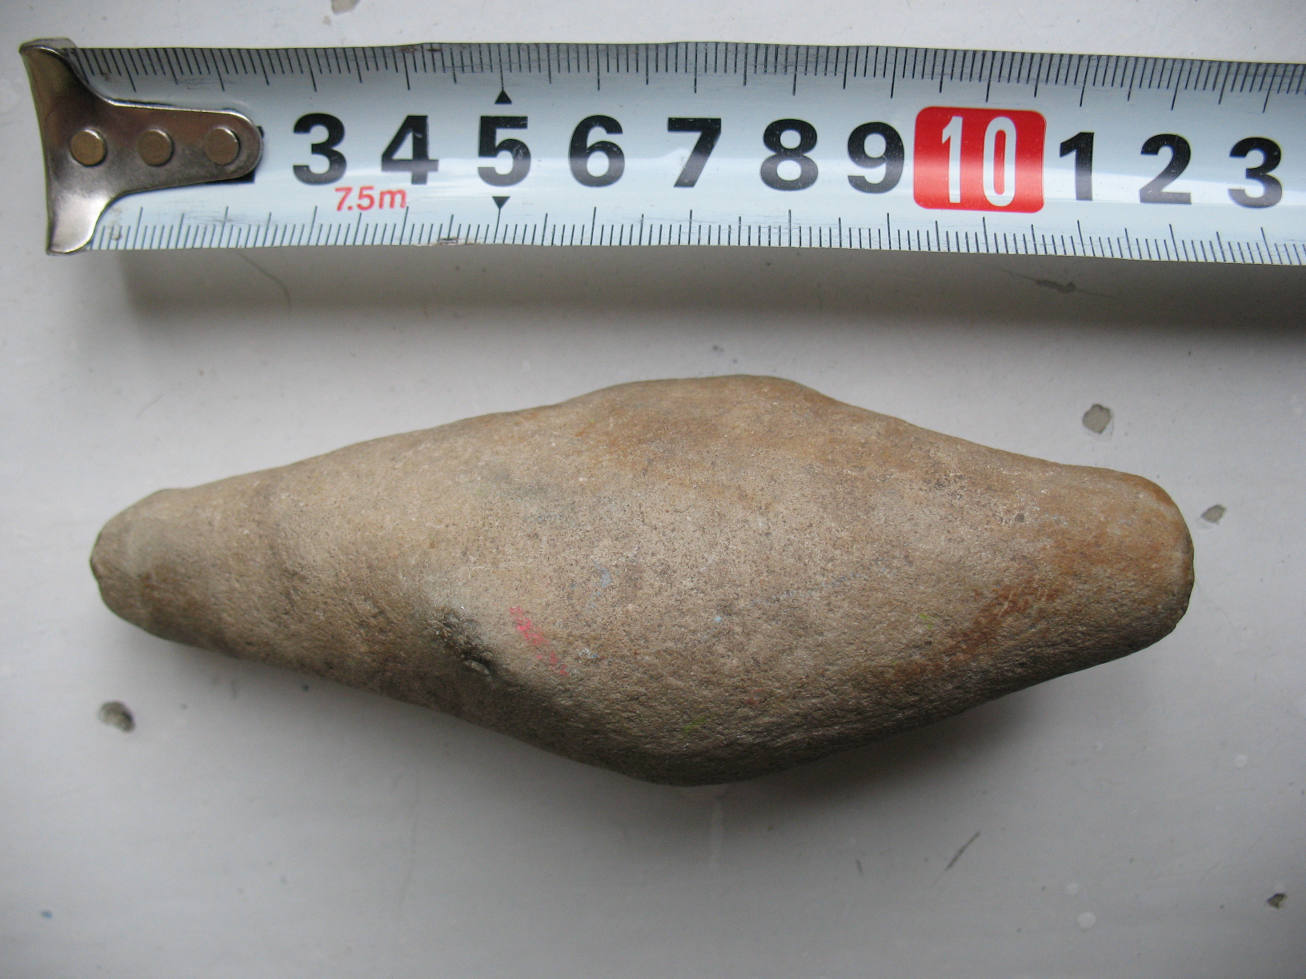
\includegraphics[width=\linewidth]{chast-colebanie-osnov/nachalo/s_figovina-01.jpg}
\end{center}

\begin{center}
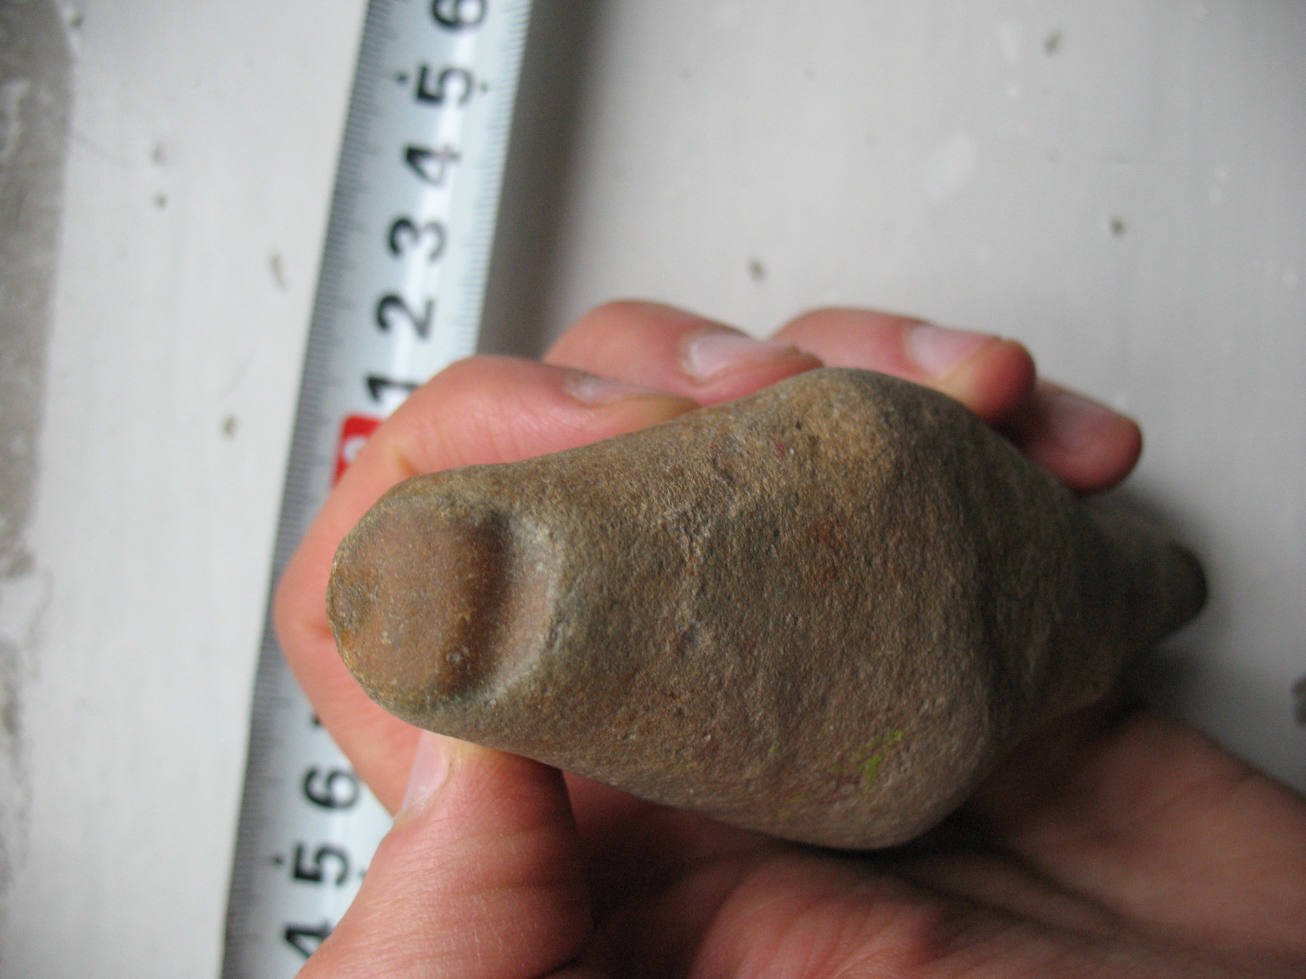
\includegraphics[width=\linewidth]{chast-colebanie-osnov/nachalo/s_figovina-02.jpg}
\end{center}
\vspace*{\fill}
\newpage

%Еще о Выдубах! В Выдубицком монастыре меня привлекала глыба базальта, черная. И глубокий колодец, могила Ушинского и прочие могилы менее именитых людей, да еще огромная ива на пригорке вне монастырских стен. Я хватался за её ветки и катался.

Расскажу подробнее, где был найден этот предмет. Мы часто гуляли «мимо ботаники», по улице Тимирязевской. С одной стороны там был бесконечный забор ботсада, увитый светло-зеленым хмелем, а с другой – захолустные усадьбы частного сектора, прорезанные сбегающими с холма проулками такими узкими, что два человека едва могли разойтись. Ниже хоздвора ботанического сада, за забором, в овраге течет ручей Омелютинка. Левый берег его, слывущий среди старожилов горой Караваевкой, высок и крут. Низовье ручья взято в коллектор. Он примерно повторяет прежний отрезок естественного русла, образовавшегося в суше после отступления вод Днепра от Зверинецкого холма.

Русло это поворачивало на север, северо-восток в сторону железнодорожной платформы Ботанической – она была на отрезке примерно между северной частью улицы Беренбойма и Деревообрабатывающей. Когда построили платформу Выдубичи, то Ботаническая загнулась и теперь о ней напоминает лишь остановка автобуса 54, и та – по требованию. Это местный маршрут, обслуживающий промзону Телички и соединяющий её с окрестностями музея Великой Отечественной войны.

На аэрофотоснимках 1943 года ручей, чуть огибая холм, впадает затем в озеро, которое было ниже Выдубицкого, отделенного от него насыпью железной дороги. Оба озера – старицы, части некогда проходившего здесь русла Днепра, рукава, что подступал под самый берег. Теперь озеро поглощено промзоной. В начале 20 века оно дотягивалось до широты конца Тимирязевской улицы, и на картах того времени обозначено как «Старик» и «Теличка», по названию местности. 

%между Зверинецкой горой и ДОКом (дерево-обрабатывающим комбинатом), и теперь поглощено промзоной. Современные границы исчезнувшего озера можно обозначить – между улицами Стройиндустрии на юге и улицей Баренбойма на севере. На одной карте Киева 1914 года озеро обозначено как «озеро Старик», на другой – как «озеро Теличка» по названии местности (деревня Теличко), причем озеро было растянуто на юг до теперешнего уровня низа улицы Тимирязевской. Стариком оно именовалось потому, что было остатками большого рукава Днепра, старым его руслом.

 %Баренбойма очень каверзная, она начинается на севере, а потом прерывается и телепортируется к метро Выдубичи!

По снимкам 1943 года видно, что от юго-восточной части озера ручей шел через пустыри и за мостом насыпи соединялся с нынешним Днепровским заливом. Сейчас ботанический отрезок ручья примечателен тем, что окрестности его кишат клещами. Некоторые участки берега, в труднодоступных местах, укреплены маленькими колышками, забота о чем прослеживается десятилетиями. Мы сняли эти укрепления в фильме «Киевская сюита», стоит посмотреть! Кто, зачем, почему?

В восьмидесятых, у самого низа улицы Тимирязевской – там сейчас сооружения тепличного хозяйства Киевзеленстроя – ручей еще не был в коллекторе, а образовывал эдакую дельту, обнятую пригорком суглинного берега. На высоте, с него гирляндами свисали засохшие ракушки нескольких видов – вроде мидий и еще каких-то длинных. Около ракушек склон казался светлым, почти белым. Встречались участки и рыжей глины – местные её копали. В небольшой пещерке невесть какого происхождения мы и нашли каменную фиговину.

Удолье у подножия холма. Островки между разветвлений ручья. Мы скакали по мягкой земле. К небу поднимались давние, громадные деревья. Из-под корней пробивался родник. Виднелись развалины частного дома, среди остатков сада росли вишни. Весной, едва пригревало солнце, появлялись цветы – фиалки, мускарики. Теплилось, веяло нерешительной свежестью. Первобытное чудесное место!

На снимке ниже, начало двухтысячных годов, может быть 2003, в дельте ручья ведется строительство. Холм частично срыт и крутизна его умерена, деревья срублены, вода загоняется в коллектор.

\vspace*{\fill}

\begin{center}
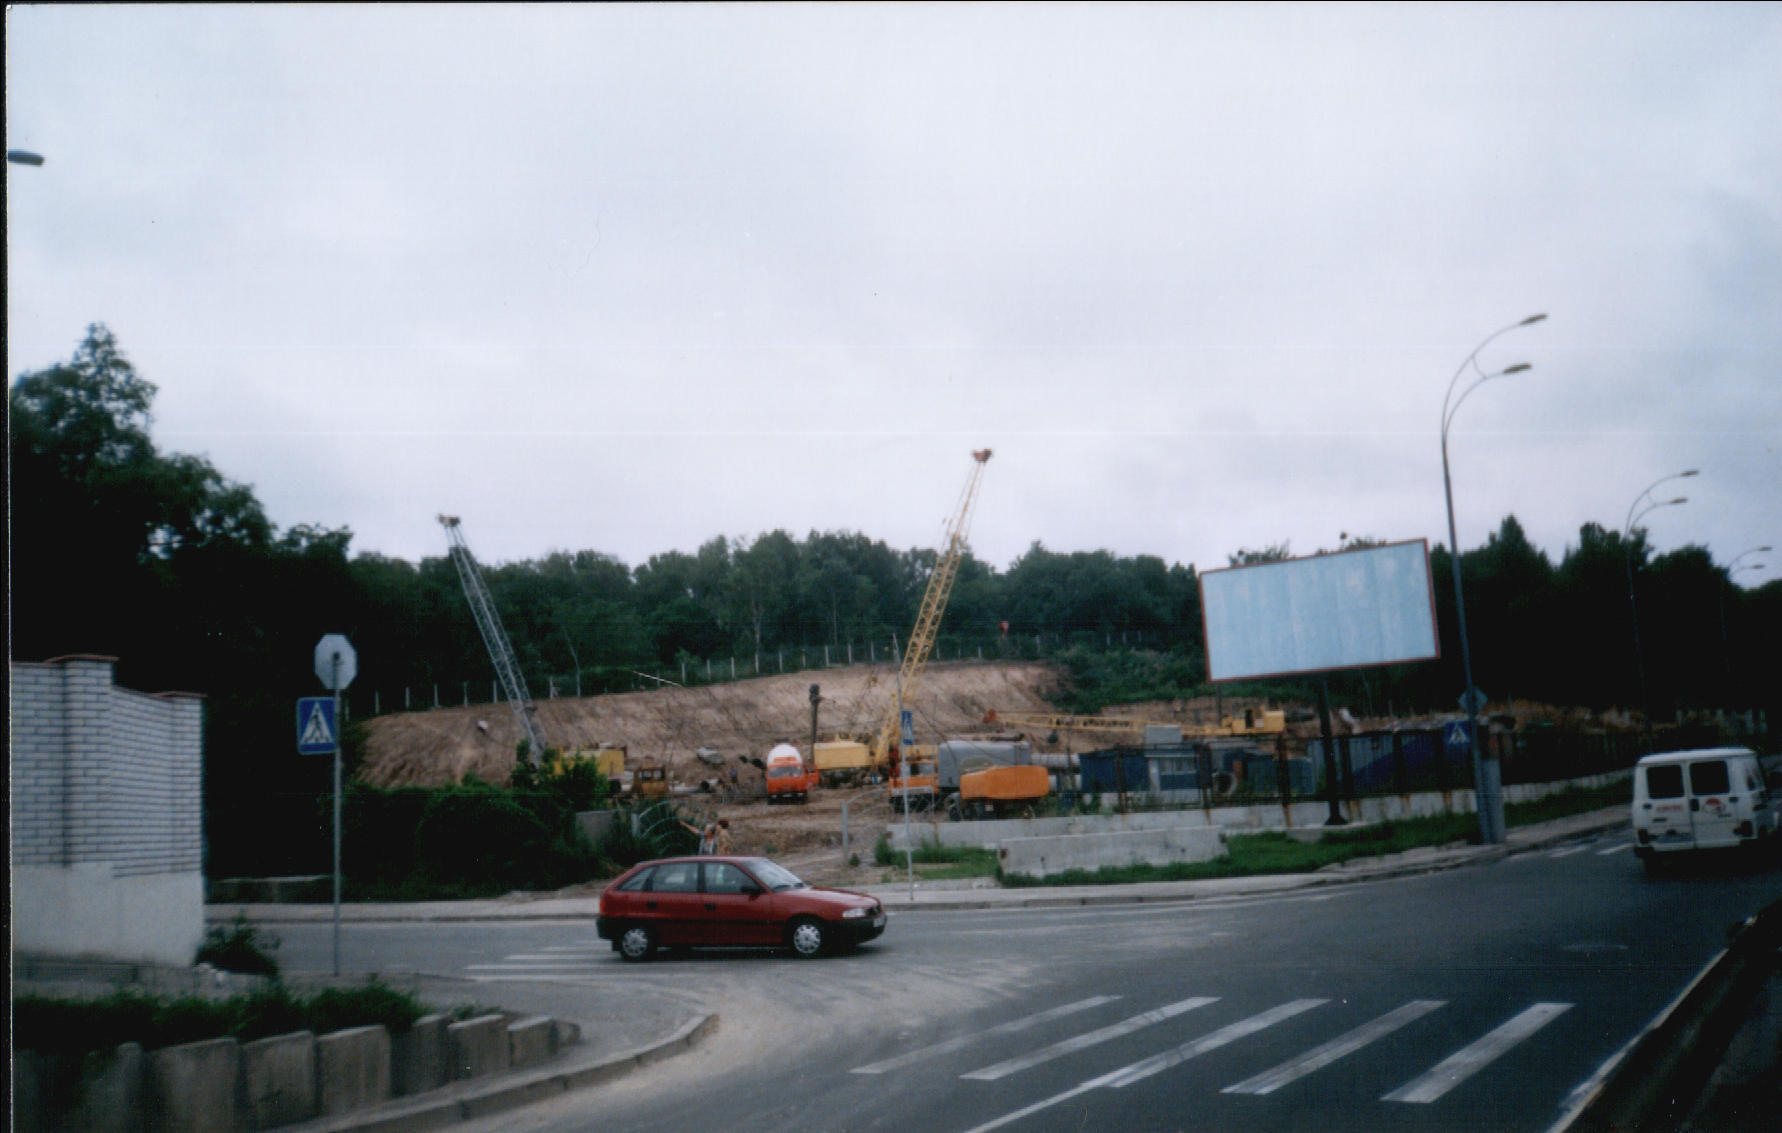
\includegraphics[width=\linewidth]{chast-colebanie-osnov/nachalo/zverinec-niz.jpg}
\end{center}

\vspace*{\fill}

\newpage

Лишь в 2016 году я, занявшись историей киевских кирпичей, узнал, что в конце 18, начале 19 веков там был карьер, где добывалась глина для кирпичного завода. При подобных обстоятельствах, когда в земле обнажаются древнейшие слои, археолог Викентий Хвойка нашел в глинище кирпичного завода Ионы Зайцева ставшую знаменитой Кирилловскую стоянку – в холме, как в слоеном пироге, один на другом покоились слои разных времен. Кости десятков мамонтов, первобытные каменные орудия.
 
А ведь если бы археологи спросили нас с мамой, где мы нашли «штуковину», коли знали б они историю местности – про завод кирпичный – сколько бы еще древностей удалось там найти? Может, «штуковина» была только ключиком к находке, сопоставимой с Кирилловской стоянкой! 

Наука безразличием похоронила открытие. Ученые сидели от него всего в полутора километрах, за толстыми монастырскими стенами. Пешком каждый день можно было ходить изучать. Но предпочитали ездить в Крым, за амфорами.

Киеву же примерно тогда же, в 1982-м, положили 1500 лет от роду, истолковав устроение Кием, братьями его да сестрой общей крепости – «града» по месту своего жительства – как основание с нуля большого поселения.

Празднование этого юбилея города я помню хуже, чем Олимпиаду 1980 года, хотя в первом случае мне было пять лет, а в последнем три. 

Про Олимпиаду встает перед глазами не её символ – олимпийский мишка, но другое. Как по той же улице Тимирязевской бегут ручьи, весной снег таять начал. А к Олимпиаде в Союзе выпустили небывалые фруктовые джемы. В маленьких квадратных коробочках. Из них получались замечательные кораблики. Я ставил в ручеек коробочку и шел рядом, наблюдая, как ее несет чуть ли не до самого хоздвора! Хоздвор знаменит. Там сеялки, веялки, теплицы и старые, выгоревшие от солнца здания сталинских времен. А по пути к нему еще магазинчик от ботсада. Продавались растения – комнатные, огородные и саженцы деревьев. Пахло цветами и черноземом.

Я не знал тогда, что чуть выше по склону, там где участок вьющихся растений, прежде было большое еврейское кладбище. Его снесли, а на месте разбили обсаженные гортензией и клематисом дорожки из бетонных плит. Среди них кое-где попадаются иудейские надгробия, по ним шагают, не замечая.

Можно пройти в самую даль участка и отведать дальневосточного крыжовника – актинидию, крупную и сладкую. Эта лиана цепляется за особую металлическую клеть-опору. Она ржавая, и столбы у навеса над скамейками тоже ржавые. Когда я лазал по ним вверх, а потом спускался, то ладони становились бурыми.

Аллеи, проходящие по бывшим улицам, скрыли прошлое. 

Напротив входа в ботсад стоит Институт проблем прочности. Раньше он раз в неделю завывал на всю округу некой опытной установкой. Местные жители и не догадываются, что всё это было огромным Братским кладбищем, где хоронили погибших в Первую мировую. И в нижней его террасе вырыты погреба хрущовок на улице Подвысоцкого. 

Нынче у меня выработалось как бы историческое зрение. Попав на местность и зная её былое, я чувствую окружающее в настоящем и смутно – в прошедшем времени. А раньше иначе. Было только настоящее и набор привычных, известных каждому, представлений. Братья Кий, Хорив и Щек, да сестра их Лыбедь. Каким-то образом, в седую старину, основали Киев...

Лет в восемнадцать я вычитал где-то цитату из «Повести временных лет» с другим вариантом основания Киева – мол, жил такой перевозчик Кий, переправлял через Днепр, и говорили – «на перевоз на Киев». Однако летописец Нестор сам же эту гипотезу опровергал.

На улице Бастионной 8/2, за углом почты, был мой любимый книжный магазин. Родной. Его после развала Советского Союза переоборудовали в стрип-клуб. В бытность книжного, одним из запомнившихся там моих приобретений начала девяностых стал репринтный томик в мягкой обложке, первого краеведа киевского, Максима Берлинского – «Краткое описание Киева».

Непривычно было «дореформенное» правописание, кажущиеся мне нескладными слова вроде «страховитый», но я прочёл книгу на одном дыхании. К сожалению, перепечатанная в ней карта Киева была махонькой и потому малополезной даже при рассмотрении через увеличительное стекло.

В «Описании» говорилось, со ссылкой на неведомого мне тогда Татищева, что сарматское слово «кивы» означает «горы». И что у впадения Десны в Днепр был город Азагориум, Загорье. Возникло противоречие – так Киев назван по имени князя Кия или от сарматского слова? И если Азагориум, при чем тут «кивы»? Я не стал решать этот вопрос. Принял к сведению, и ладно.

В конце девяностых в Киеве, близ станции метро Петровка, появился одноименный книжный рынок. Туда поначалу переселились торговцы с прежнего, еще «перестроечного», рожденного в 1989 году книжного базара на Куренёвском, или Птичьем рынке. Впрочем, на Птичке по нулевые, не знаю как сейчас (давно не был), существовала небольшая букинистическая толкучка. Со временем на Петровке стали продавать диски с музыкой, программами, фильмами, а затем там образовалась и барахолка как на Куренёвке – да кстати Петровка не так уж далека от нее.

Раньше я часто посещал Петровку, а нынче езжу редко. Покупаю там на букинистических раскладках, в основном где старые книги разложены прямо на асфальте или как щенки-дворняжки выглядывают из коробки. Бывало, возвращался домой с полным рюкзаком, набитым дешевыми и ценными для меня изданиями.

Но миновали светлые времена. Чудесные россыпи хороших подержанных книг по копеечной цене превратились, большей частью, в скопления быстро пожелтевшей перестроечной кооперативной и современной макулатуры.

И вот однажды, когда мой интерес к киевоведению только просыпался, я взял на Петровке книжку в мягкой серой обложке, «Древняя Русь и Киев в летописных преданиях и легендах», Николая Федоровича Котляра. Киев, Наукова думка, 1986 год, цена 30 копеек, 160 страниц, тираж 70000. Современные писатели, завидуйте размаху советской книгопечати.

В работе Котляра я наткнулся на любопытную выдержку, впрочем прерываемую сочинителем и предваренную его оценкой – «встречаем забавную историю, выдуманную, скорее всего, в Новгороде».

А речь шла о том, что Кий, Хорив, Щек и сестра их Лыбедь были разбойниками из Новгорода.

\chapter{Загадки Повести временных лет}

Официальная история не любит новгородцев-летопис\-цев. Подобно тому, как в старинной пословице «Орел да Кромы – первые воры» больш\'ая часть населения этих городов приравнивается к ворам, новгородских летописцев считают обманщиками, выдумщиками.

 %Дружно хохочут историки над сочинениями новгородских летописцев. А может и не дружно, а наедине. Если в библиотеке вдруг раздается неуемный смех, он наверняка исходит от историка с третьим томом Полного Собрания Русских Летописей.

На полке у каждого киеведа зачем-то стоит зеленое, 1982 года издания четырехкнижие «История Киева», подготовленное коллективом ученых. Там сказано, что в отличие от киевской «Повести временных лет», летописцы новгородские прямо сообщают дату возникновения Киева. «Но ей нельзя доверять» – сурово поднимает палец наука. А почему? Поясняют: «Она была внесена в рассказ о Кие новгородскими летописцами XI-XII веков, пытавшимися создать свою схему исторического развития Руси, в которой не Киев, а Новгород выступил бы наиболее ранним восточнославянским городом».

Однако, на основании чего мы должны принять, что новгородцы врут? Лишь потому, что они новгородцы и у них «своя схема»?

Впрочем, некоторых историков уже несколько веков не устраивает и предание об основании Киева легендарными братьями. Красивая выдумка! Не было таких братьев, этимологический миф.

Объявите что угодно враньем и пол\'учите возможность бесконечно утверждать новые истины.

А мне кажется правдоподобным, что некогда живущие родичи Кий, Хорив, Щек и сестра их Лыбедь сообща основали укрепленное поселение на холмах нынешнего Киева. Но кто они, откуда взялись?

Котляр не указал источник выдержки о разбойном семействе. А у меня оно в голове застряло. Но погрузиться в изучение летописей я не отваживался много лет. Тем и довольствовался, что Котляр выписал. Однако сомнение было посеяно.

И наконец я понял – пора самому читать летописи. Но и в известнейших не было про этих разбойников. Нашлось в малоизвестных списках. 

Слово «список» буквально означает копию, нечто списанное с подлинника. К сожалению, из русского языка исконный смысл «списка» вытеснен прямым латинским переводом, словом «копия».

Благодаря этому излишеству, мы привыкли под «списком» разуметь другое – строчки с перечислением, например товаров либо имен. Применительно к историческим и литературным источникам, «список» это рукописная копия (порой исправленная, неполная, или дополненная) летописи либо иного произведения.

Существуют различные летописи и списки оных, отличающиеся подробностями изложения событий, но порой и в корневых предметах. Важнейшие и приемлемые различия, при издании, обычно выносят в приложения или примечания, дабы читатель мог сравнить этот список с другими.

Федор Александрович Гиляров (1841-1895) подготовил и выпустил целый сборник таких примечаний, «Предания Русской Начальной летописи (по 969 год). Прилож\-ения»\cite{gilyarov01}, взяв за основу «Повесть временных лет» по Лаврентьевскому списку, датируемому 14 веком. 

«Повесть» – сборник наиболее ранних преданий о Руси, составленный, как издавна считалось, летописцем Нестором из разных источников. Обычно включается в начало «главных» летописей. Кроме Нестора, в 1116-м над «Повестью временных лет», о чем можно судить по указаниям в ряде списков, потрудился игумен Выдубицкого монастыря Сильвестр. Диву даюсь, что двадцать лет прожил рядом с местом, где это происходило, да и до Лавры недалече.

Вопрос авторства текста, известного как «Повесть временных лет», остается открытым. Первоисточник до наших дней не дошел. У нас нет рукописи ни пера Нестора, ни Сильвестра. В позднейших копиях разнобой. Например, в Хлебниковском списке 16 века составителем значится Нестор, но не указан Сильвестр. В Лаврентьевском и еще двух списках 14-15 веков, после окончания текста записью за 1110 год, добавлено «Игумен Селивестр святого Михаила написах книгы си летописец, надеяся от Бога милость прияти, при князи Володимере\footnote(Мономахе), княжащю ему в Кыеве, а мне в то время игуменящу у Св. Михаила в 6624, Индикта 9 лета; а иже чтет книгы си, то буди ми в молитвах». Так ли это и каким образом соотносится с Нестором –  проверить нельзя. Исследователи строят разные предположения.

Для простоты я бы считал, что Нестор на основе ряда источников (и часть их точно установлена) и собственных впечатлений написал «Повесть», а затем ее правил Сильвестр. Насколько эта простота истинна, сказать не могу. Некоторые ученые, стремясь предать Нестора забвению, полагают, что Сильвестр сначала был иноком в Лавре, а после сделался игумном в Выдубичах.

Как бы ни было, чтение «Повести» приводит к мысли, что за ней стоял, исходно, некий любознательный монах Лавры, одновременно краевед, и по крайней мере в 1106 году он был еще жив. Спустя более столетия, между 1224-1231 годами, лаврский монах Поликарп писал архимандриту Акиндину про Нестора, указывая «иже написа летописец», то бишь в церковной среде в то время уже был известен «летописец» (слово это обозначало летопись) – подразумевается, положим, именно «Повесть» – и Поликарп связывает ее с Нестором.

Существуют однако кое-какие сюжетные противоречия между «Повестью» и приписываемым Нестору житием преподобного Феодосия, а также сказанием о святых князьях Борисе и Глебе. То есть, можно разбирать доводы за и против. Вот, в пещерах Лавры покоятся мощи Нестора Летописца. Именно под таким прозвищем он слывет, подвторюсь, издревле. Но известен есть и другой Нестор, Некнижный, следовательно первый Нестор отличался именно своей образованностью. 

Возможно, в будущем я попробую решить задачу сочинительства «Повести временных лет», однако не сейчас.
 
Так вот Гиляров, в своей книге, для каждого раздела «Повести» привел описание тех же событий по летописям Новгородской, Псковской и прочим источникам, включая польские. Гиляров поместил много архивных редкостей, что еще более усиливает значение его труда, да и пожалуй является главной ценностью оного.

С шестидесятой страницы «Приложений» открываются чудеса про основателей Киева.

Книга Гилярова меня словно разбудила и сбила с толку. Как же, чему верить? Странны и противоречивы оказались списки. Одно дело, когда различия летописей встречаются отдельно и с перерывами. Словно редкая капля дождя – оросила лицо, ощутил, да идешь дальше. А у Гилярова это огромное собрание таких различий, уже даже не дождь, но вся небесная вода, упавшая на землю и собравшаяся в один поток, что уносит прочь от привычных представлений!

Известные князья, разведенные официальной историей по времени, здесь оказываются действующими вместе. Появляются новые их родичи. События переносятся в другое время и место, а участвуют в них совсем другие люди. 

Что же историки, археологи? Осведомлены о вариантах истории? Это у них надо спрашивать. Сами они в книжках ничего такого не говорят, а если даже что прорывается, то с оговоркой, вроде как у Котляра – забавная выдумка!

Общепринятая история – лишь один из вариантов, однако об этом молчат. Ученые решили, исходя из своих представлений о прошлом, считать истиной сведения только из определенных списков. Можно проверить таблицу умножения. Но давний летописный слой событий нельзя – начинается путаница. С нею столкнется любой, кто примется за такой труд.

А наука это храм. Строится из кирпичей. Кирпич должен быть однозначным. Чтобы всякий взял его в руку и признал – это кирпич. Кирпич клеймлён именем князя да годом рождения. Вот еще кирпич, тоже с именем и годом. Положим их рядом на цемент. Два князя вместе. Основа готова.

Однако нельзя точно сказать, что на кирпичах должны быть именно эти имена и числа. Но ученым нужно строить. И они делают кирпичи. Приходится одни имена и годы признавать истинными, другие ложными. Таков научный подход – отставив сомнения в сторону, возводить лишь одно здание. Вместо нескольких, поменьше высотой, зато с разными наборами кирпичей.

Основание огромного здания пересмотру не подлежит. Замена разрушит всё здание. Общепринятые представления об истории это цемент научных работ. Изъятие цемента приведет к распаду.

Если хочешь быть ученым в среде официальной науки, необходимо участвовать в общем строительстве единственного и нерушимого её храма. Делай новые кирпичи, клади цемент, возводи ряд за рядом новый этаж. Не подходит кирпич? Выкинуть! И не сомневайся. Правда за нами!

Вошедшее в «Приложения» Гилярова – выкинуто. Этого будто нет. Не должно быть. Иначе научные труды – в последние годы ставшие смесью взаимных ссылок – потеряют целостность, а журналисты будут вынуждены делать трудный выбор, что же писать о незнакомом предмете.

Официальная наука история и ее противники, та же «новая хронология», больше тратят сил насаждая истину, нежели выясняя оную. Утверждают – было так, а не иначе. Или, еще проще – было так. Без иначе. Умолчать. Когда не получается, обязательно указать – ошибочное мнение.

В семидесятых наконец издали первую часть «Пространной истории города Киева с топографическим его описанием» Берлинского, которую при жизни он в печати не дождался. Добро, ну так опубликуйте с уважением. Читаю.  Вот Берлинский пишет, вероятно следом за Татищевым, что вместо Аскольда и Дира был один человек, «Аскольд тирарь». Сразу примечание редактора – Берлинский конечно ошибается!

Наука, словно ползающий на коленях Хома Брут, чертит по полу колдовской круг с шептанием – Берлинский ошибается, новгородские книжники врут, этой дате безусловно нельзя доверять. И перестает быть наукой, ибо наука это изучение, а изучение прекращается, когда нет сомнений.

Но внутри науки, коли хочешь в ней обретаться, не остается ничего другого, как принимать ее правила игры. Не зря Гиляров вспоминал в своих заметках\footnote{Что печатались из номера в номер «Русского Архива» за 1904 год.}, наставление:

\begin{quotation}
«Не всегда говори, что мыслишь; знай больше, а говори меньше» и т.д. Достоинство этих истин оценено было мною, конечно, уже много лет спустя по их изучении.
\end{quotation}

Сын священника Московского Новодевичьего монастыря\footnote{Фамилию Гиляров священник получил от начальства духовного училища, как прозвище – в переводе с латыни «hilaris» значит «веселый». Александр Петрович Гиляров – старший брат Никиты Петровича Гилярова-Платонова.}, Федор Александрович Гиляров учился поначалу в Московской духовной семинарии, откуда был вытурен за статью «Материалы для физиологии общества»\footnote{«Московские Ведомости», 1859, № 62.} и пошел по светской стезе, поступив на историко-филологи\-ческий факультет Московского университета\footnote{Там же учился историк Ключевский, они с Гиляровым были приятелями еще в бытность последнего семинаристом.}. 

Окончив курс в 1866-м, пятнадцать лет преподавал русский язык в различных учреждениях, попутно выпуская одну за другой работы по истории, языку, краеведческие исследования. Среди них наиболее известным трудом была «Этимология Русского языка», составленная совместно с Александром Ивановичем Кирпичниковым. Перу Гилярова принадлежат также «Этимология Церковнославянского языка», «Русская хрестоматия для низших классов гимназий», «Исторические и поэтические сказания о Русской земле в хронологическом порядке событий», азбука для сельских школ «Школа родного языка», «15 лет крамолы» и другие. Всё это нынче днем с огнем не сыщешь.

Гиляров умел, кажется, выбирать самые неудобные предметы для своих работ. Названия его трудов порой даже боялись верно писать в библиографиях – искажали и название, и год выхода в печать, чтобы сбить с толку цензуру.

В 1883 году Гиляров выпустил, на основе своих статей в «Современных известиях»\footnote{Оные издавал дядя Гилярова, Николай Гиляров-Платонов. Федор Гиляров состоял там вторым редактором. Оба Гилярова слыли, по словам Владимира Алексеевича Гиляровского, людьми «не от мира сего». В типографии «Современных известий» вышли и «Приложения русской начальной летописи».}, книгу «15 лет крамолы (4 апреля 1866 г. – 1 марта 1881 г.)» о революционном движении в России. Отпечатанный трехтысячный тираж первой части первого тома – «Пропаганда. (4 апреля 1866 г. – 24 января 1878 г.)» – был запрещен спохватившейся цензурой под предлогом «исключительной важности предмета книги и его щекотливости»\footnote{См. Сводный каталог русской нелегальной и запрещенной печати. М., 1971. Ч. I. С. 149.}. Название оказалось пророческим. 15 лет книги лежали в закромах под арестом, от сырости 2500 штук истлели, оставшиеся поныне считаются редкостью.

В том же 1883 году выйдя в отставку, Гиляров начал печатать свою газету, «Афиши и объявления», позже переименованную в «Вестник литературный, политический, научный и художественный». Издание освещало большей частью театральную жизнь. Современник с похожей фамилией, Владимир Гиляровский вспоминал в «Москве газетной», что «Федор Александрович писал недурные театральные рецензии, а затем сам издавал какой-то театральный листок, на котором прогорел вдребезги».

Скончался Гиляров в Химках под Москвой, в 1895 году. Похоронен в самой Москве на Пятницком кладбище.

Зачем я рассказал о нем относительно подробно? Дабы за отсылками к источнику, важному в моей книге, стоял человек, а не имя. И если о человеке нынче мало помнят, стоит напомнить, что был такой, и каким он был.

Гиляров вытащил из архивов в печать наиболее яркие «отклонения» от общеизвестных списков\footnote{Подобное, но в меньшем объеме, либо пересказе, и с выраженной оценкой можно найти еще в работах Михаила Николаевича Тихомирова (1893-1965), например в  его «Кратких заметках о летописных произведениях в рукописных собраниях Москвы», изданной в 1962 году.} – то, что ученые предпочитают, если знают, замалчивать. А с несведущих и спроса нет. «Приложения» могли бы перевернуть представления о ходе истории. Но куда там! Эта книга ведь целая дорога, усыпанная камнями, о которые каждый споткнется, коли не захочет обойти.

Науке бы чего попроще! Гладкий асфальт. Но помимо редких списков, даже основные летописи задают такие загадки, ответы на которые разрушат здание современной науки истории. Посему, да по неведению, эти вопросы обычно не поднимают. А мы поднимем. 

\chapter{Так говорят летописи}

Кстати, а на каком языке велись летописи?

Ученые толком не отвечают, но поясняют, что это не был разговорный язык, и на Руси в старину так не говорили. А дескать, Кирилл и Мефодий разработали на основе своего родного языка литературный. И его-то нынче и называют церковнославянским или старославянским. Насколько это представление науки справедливо, мы исследуем ниже.

В каждой летописи с веками накопилась уйма правок, включая языковые. А язык меняется в зависимости от местности и с течением времени. Правщики летописей, переписывая оные, в некоторой мере осовременивали их и придавали местный оттенок. В меньшей степени это коснулось религиозных книг.

Но рассудим, какой толк в мысли, утверждаемой наукой – церковнославянский никогда не был на Руси разговорным языком. Для кого же тогда переводить на него религиозные произведения и вести на нем летописи? Зачем создавать на нем новые произведения?

Ответ прост. Ученые ошибаются. Это и был, в какое-то время, разговорный язык, общий для Славян, тогда еще не столь разрозненных и разнящихся, как сейчас. И благодаря упорному держанию традиций, православная церковь сохранила нам, по большому счету, древний разговорный язык в том числе и Киевской Руси.

Однако, начиная с некоего времени, в разных местностях по-разному, разговорный язык стал меняться быстрее, чем «церковный», чем язык священных книг. В итоге язык обиходный и книжный таки друг от друга отделились. Ведь язык «церковный» был привязан к религиозным сочинениям, а мы помним, как правка даже в рамках «церковного» языка богослужебных книг при патриархе Никоне послужила одной из причина Раскола в православной церкви, и доднесь (хорошее, старинное слово) многие старой веры держатся, ибо не приемлют правок, внесенных при Никоне и в последующие годы.

Давний, общеславянский язык – такой же, как летописный, используется в многочисленных житиях святых, поучениях и подобных сочинения. Да и сами летописи ведь не однородное перечисление событий, а смесь выдержек из источников светских и духовных.

Но обратимся к другим видам письменности. Обиходный, не церковный язык должен быть запечатлен в граффити на древних стенах, в пещерах, в сводах законов наконец.

Возьмем надписи на стенах Софии Киевской\footnote{Неизбежно встает вопрос о грамотности населения времен Киевской Руси. Для кого делались надписи на пряслах (грузках для веретен)? Надписи в пещерах Лавры? А на кувшинах? Известны текстовые клейма на кирпичах, посуде и так далее, причем по-славянски и вроде бы по-гречески. Значит, грамотен был народ, и не токмо славянской грамоте разумел! Между тем знаменитый Оттон Первый Великий – король Германии, император Священной Римской империи, читать выучился лишь на сорок шестом году жизни. И то хорошо! Другие тогдашние правители из просвещенной Западной Европы крестами подписывались.}. Это тот же язык, что в летописях и давних церковных книгах. Переводы греческой литературы, например «Временника» монаха 9 столетия Георгия Амартола – тот же язык. Свод законов «Русская правда» (Правда Роськая)\footnote{Примечательны строки в ней, где говорится, кто утвердил этот свод законов: «Правда оуставлена Роуськой земли, егда ся съвокоупил Изяслав, Всеволод, Святослав, Коснячко, Перенег, Микыфор Кыянин, Чюдин, Микула».}, по списку 12 века – тот же язык, хотя ученые утверждают обратное. Впрочем, ныне вольно проверить любому желающему! Берестяные грамоты из Новгорода – тот же язык. «Хождение за три моря» Афанасия Никитина, берите еще, черпайте полной горстью давние сочинения – один язык! Безусловно, при сравнении этих разнородных источников обнаруживается некоторая разница – ибо  источники разнесены по месту и времени.

Но в целом же, в единости языка древнего обиходного, летописного и «церковного» может убедиться каждый, кто собственными глазами прочтет первоисточники.
 
Вот английский язык допустим 16 века, сравните с английским 19 века – между ними очевидная разница. Но ведь ученые не утверждают при этом, что англичане в 16 веке говорили на каком-то другом языке, чем отраженный в произведениях того времени. Нет, принимается за должное, что был такой язык, как в книгах.

А про старославянский нам навязывают примерно такую мысль – это был язык священный, на Руси его не использовали вне церковной литературы, обиходный же язык был другим. При этом ученые видят светские «Роськую правду», берестяные грамоты, граффити – видят там старославянский, и какой делают вывод? А довольно странный. Дескать, это разговорный язык, но с примесью церковнославянского. Лишь бы не признавать, что старославянский и был разговорным!

%Обходят стороной и использование старославянского в лубочных картинках, сопровождаемых пояснительными письменами. Был лубок религиозный – со сценами из Библии и житий святых, сатирический, исторический, срамной, шутейный, поучительный, колдовской и прочих жанров. Даже в девятнадцатом веке и начале двадцатого на лубке сплошь и рядом находим надписи на «церковнославянском».

%Примеры. Лубок «Птица Сирин святаго и блаженнаго рая». Подпись: «Аще человек глас ея услышит, пленится мысльми и забудет вся временная и дотоле ж лед тоя ходит, доднеже пад умирает, глас ея слышати не престает». Возле головы птицы: «Видом и гласом».

%Лубок «Наказание Людвику Ланграфу за грех стяжания», конец 19 столетия. Полное название оного лубка: «Книга мирозрительное зерцало, глава 257. Стяжание неправедно, стяжани дерзнув некий ланграф, терпяше велие мучение адское». Кусок текста оттуда: «Людвик ланграф великий мучитель, людей [...] токмо аз и сынове мои. Той же прият знамение, а ланграфа ввергоша в бездну, и возврати диавол клирика». 

%\begin{center}
%\includegraphics[width=0.75\linewidth]{osn-kiev/hristofor.jpg}

%\textit{Лубок. Песиголовец святой Христофор.}
%\end{center}

%Лубок начала 20 века, «Зерцало великое, глава 138. Яко напрасно нам виновен бес бывает». Его текст: «У некоего пустынника молитвою связан бысть бес, и стрежаше репу его. И некогда прииде человек к старцу репы [...] ради от своей мысли смущен бых, и абие простив отпусти его старец с репою, яко невиновен нам бес делом, но мыслию точию».

%Сообщения о памятных исторических событиях, явлениях чудес и дивных зверей в заморских странах, притчи, молитвы – всё это выпускалось для народа на лубке, записанное языком, который ученые считают чисто книжным и церковным! По лубку видно, что язык русский литературный, язык Пушкина, скажем так – хотя встречается на лубке, однако на позднем, и то в меньшей степени, нежели старославянский.

%Конечно, у нас есть сборники былин и народных песен, донесшие обиходный русский язык 19 века – он близок к «пушкинскому», но вспомним, что лубок писался понятным народу языком, и лубок выпускался исходя из спроса. Следовательно, был спрос на лубок с текстами на старославянском, а не «современном».

%Можно возразить – спрос такой потому, что грамоте учили в церковных школах, или дьячки нанятые. Дескать, что сами знали, тому и обучали. Казенных школ для простого народа, помимо Василия Татищева ох как долго никто не заводил, просвещением занималась таки церковь. Но даже в начале 20 века «церковный» язык в письменности, был, кажется, вполне понятен грамотной части народа одновременно с обиходным.

Русский язык 19 века еще сохраняет много общего с давним – окончания вроде «ою» вместо «ой» (водою, водой), «противу» вместо «против», да много чего. В украинском поныне используются окончания «ою», слово «як» (было «яко», в русском стало «как»), славянские имена месяцев и так далее. Оба языка еще не утратили древнего звучания, однако изменились относительно исходного. 

А вот современный болгарский похож на старославянский значительно меньше, чем русский и украинский, хотя языковеды утверждают, что церковнославянский возник на основе некоего «южноболгарского». Здесь языковеды сами себе противоречат, ибо они строят дерево происхождения языков на сравнении их сходства, и в случае со старославянским идут вразрез со своими же правилами. 


%А ведь разные степени сходства означают всего-то, что на землях нынешней Украины и России, славянский язык изменился – от исходного старославянского – менее, чем в землях, занимаемых Болгарией. И что в определенное время старославянский был родным обиходным языком населения этих земель.


Но что значит «Болгария»? В давнее время была известна другая Болгария, о ней много писали Арабы, а ее население современная наука объявила тюркским. Это Болгария на реке Волга.

Слова меняются по звукам, которые могут произноситься нечетко. «Б» легко становится «в», «о» – «у», твердое «г» превращается в мягкое «х» и звонкое «к». Иногда звуки просто выпадают из слов.

Возьмем корень Болгарии. Болга. Что это? Волга. Что говорит летопись про Болгар? Далее отрывок из Ипатьевского списка, где говорится про язык (язык в значении ветвь народа, а не набор слов\footnote{Современные учебники церковнославянского сообщают, что слово «язык» в значении народа пишется с буквы «я», а в значении языка, набора слов и правил их построения – с буквы «юса малого». Однако в старинных книгах мы видим безразличие к этому, и «язык» в значении «народ», «ветвь народа» пишут как с «я», так и с «юса малого».}) под именем Словене (Славяне), который жил на Дунае:

\begin{quotation} 
Словеньску же языку, якоже ркохом живущю на Дунаи, придоша от Скуфь, рекше от Козар, рекомии Болгаре, и седоша по Дунаеви, насильнице Словеном беша. А по сем придоша Угре Белии, и наследиша землю Словеньскую, прогнавше Волохы, иже беша преже прияле землю Словеньску
\end{quotation} 

%Любопытствующие могут почитать вне этой книги, кем полагают ученые Волохов, Скифов, Козар и других. Я же даю свою трактовку, основанную на источниках, а не домыслах.

Что сказано в летописи? К тем Славянам, жившим на Дунае, от Скифов, говорят от Козар\footnote{От Козар из числа Скифов. То бишь, есть разные Скифы, а среди них Козаре.} – явились Болгары, насильно поселившись там. После этого пришли Белые Угры, и наследовали землю Словенскую, прогнав Волохов – Болгар, которые перед этим захватили (прияле) землю Словен.

Летопись прямо называет Болгар Волохами. У Болгар и Волохов общий корень – Волга, учитывая замену звуков! А как вы думаете, что лежит в основе названия Балканы?

Наука не понимает тождества давних Волохов и Болгар, не видит соседства Валахии (часть нынешней Румынии) и Болгарии. Не замечают также сходства Болгар с названием народов Белгов (от этого «Бельгия») и Фир Болг.

%Но если, по мнению ученых, старославянский язык основан на «южноболгарском», то, продолжая цепочку рассуждений и приняв летописное утверждение, что Болгары пришли с Поволжья, следует вывод, что на Поволжье пользовались тем же языком!

О Козарах. Здесь и далее я всюду пишу Козаре, вместо Хазары, следуя давнему написанию. В латинских же источниках встречаем – Cazari. У Греков, однако, с буквы «х».

Наука считает Козар тюрками, популярная культура приписываем всем Козарам исповедование иудаизма. Я же приведу, что написано о Козарах в «Житии и трудах преподобных отцов наших Мефодия и Константина-Кирилла, учителей словенских» Дмитрия Ростовского, по лаврскому изданию 1764 года. Можно считать это мнение срезом тогдашних представлений о Козарах:

\begin{quotation}
Козары, их же Грецы Хазарами, Римляне же Газарами нарицаху, бяше народ Скифский, языка Славенскаго или Российскаго, страна же их бе близ Меотийскаго езера\footnote{Азовское море.}, еже и Мертвым морем нарицается, в неже Дон река Азию и Европы разделяющая впадает [...]

племя некое Скифское, глаголемое (от гор Аланских) Аланы, прозванныи же потом (от реки Козара именуемой) Козары, седе и долгими временами расплодися зело, и населяшеся по обоим странам Дона, ово во Азии, даже до Волги в Каспийское или Хвалынское море впадающей; ово же и во Европе, даже до Днепра в Черное море входящего. [...]

ибо и до Паннонии досягоша, но оуже тамо иными нарицаниями прозвани быша, ово Авары, ово Гунны, и во иные пременишася народы.
\end{quotation}

По некоторым «житиям» картина несколько иная, и Козаре предстают не однородными Славянами, но сообществом различных народов, где помимо славянского в ходу язык, именуемый в давних источниках «жидовским»  или «самаритянским».

Мне любопытно сталкивать мнения современной науки с общепринятыми представлениями прежних веков. Любопытна и связь Козар с Аланами, ведь известно, что в определенное данниками Козар была Киевщина и многие окрестные земли, а ведомо также, что эти же земли были примерно тогда же подвластны славянскому народу Полянам. Достаточно отбросить от Полян букву П, и мы получим тех же Аланов.

В наших летописях Поляне упомянуты кратко, а переподчинение Вещим Олегом земель, платящих дань Козарам, сокращено еще более, будто не возникало при этом никакого недовольства со стороны Козар, теряющих одно владение за другим. Можно сказать, что Козар летописных не существует вовсе, вместо них пробелы, дыры в истории, вырванные места.

В летописях, однако, мы не встречаем отождествления Козар с Полянами. Более того, согласно Повести временных лет, после смерти Кия, Хорива и Щека, Полян обижают Древляне да прочие окрестные народы, а Козаре, живущие «в лесех на горах», пытаются обложить Полян данью, на что Поляне платят по обоюдоострому мечу с каждого двора.

Главу Козар называли «коган», или, как нынче любят писать, «каган». Учитывая мягкость давнего «г», можно предположить, что при самих Козарах это произносилось как «кохан». В украинском языке сохранилось слово «кохання», любовь. Вплоть до 16 века на Руси было множество должностей, связанных со словом «излюбленный» – «излюбленные» старосты, головы, судьи. Излюбленный означало – избранный, выборный. Возможно, таково же и значение козарского «кохана», если Козаре были от «языка славенского».

Я не берусь здесь разбираться в противоречиях между житиями и летописями и выяснять происхождение Козар. Мне кажется, что это название жителей разнообразного по народностям государства, исповедовавших различные религии. В одно время верхушка Козар исповедовала иудаизм, в иное время – христианство. Пожалуй это про Козар всё, о чем можно судить точно.

В Киеве, по летописям известен район города – Козаре – его иногда отождествляют с другим районом, Жидове, однако нет прямого указания на такое отождествление. Значит, в Киеве времен «великокняжеских» Козаре обосабливались среди прочего населения, но чем занимались и какую играли роль, неведомо.

Теперь относительно Кирилла и Мефодия, точнее Константина (Кириллом он стал, приняв схиму) и Мефодия, деятельных братьев из Солуни\footnote{Селунь, Солунь – греческий город Салоники.}, с которыми принято связывать изобретение славянской письменности, алфавита, когда из Моравии поступил запрос на понятную народу Библию, не греческую, не латинскую, но славянскую.

До революции 1917 года, тексты летописей были доступны немногим, да и в советское время переиздавались нечасто. Для работы с ними приходилось ездить в библиотеки Москвы, Киева или Ленинграда, большинство же исследователей довольствовалось разрозненными цитатами, переходящими из книги в книгу, и осовремененными «переводами» летописей, в частности Повести временных лет.

Хрестоматийный перевод Повести временных лет, выполненный Дмитрием Лихачевым, в месте про Кирилла и Мефодия, гласит: 

\begin{quotation}
Был един народ славянский: славяне, которые сидели по Дунаю, покоренные уграми, и моравы, и чехи, и поляки, и поляне, которые теперь зовутся русь. Для них ведь, моравов, первых созданы буквы, названные славянской грамотой; эта же грамота и у русских, и у болгар дунайских. 
\end{quotation}

Открываем подлинник по Лаврентьевскому списку, за 6406 год от сотворения мира:

\begin{quotation}
бе един язык Словенеск. Словени же седяху по Дунаеви ихже прияша Оугри и Марава Чеси и Ляхове и Поляне яже ныне зовомая Русь сим бо первое преложены книги Мараве. яже презвася грамота Словеньская. яже грамота есть в Руси и в Болгаре Дунаиских.
\end{quotation}

Где тут написано про создание букв? Откуда Лихачев взял, что для Моравов\footnote{Кстати, Моравы сами себя еще в 19 веке именовали Чехами. Моравами их называли чужестранцы.} первых созданы буквы, названные словенской (славянской) грамотой?

Подлинник ясно говорит – книги (а речь идет о священных христианских книгах, Библии) сперва были «преложены» – переведены – народу Мараве. 

Эти-то переводы называли грамотой Словенской, Писанием Словенским. Опять-таки летописец подразумевает Библию, на Словенском. И дополняет, что такое Писание в ходу в Руси и у Болгар Дунайских. 

Примечательно – еще с 19 века исследователи заметили, что в старейших редакциях житий святых Кирилла и Мефодия на старославянском, сказано «книги», а в поздних «книги» постепенно превращаются в «письмена». Несмотря на это, наука считает Кирилла и Мефодия создателями славянской азбуки, а однго из двух алфавитов – кириллицы и глаголицы, еще не определились какого, но застолбили на всякий случай оба.

Именно «письмена», или даже «грамота», упомянуты в единственных на греческом языке сочинениях, касаемых Константина и Мефодия – вариантах жития святого Климента, где есть «граммата Скловениха». И слово «γράμματα» («граммата») обычно переводят как «буквы», совершенно выпуская из виду, что оно обозначает и письмо в смысле Писание, священные книги. Так, на греческом, Iερά Γράμματα – Иэра Граммата, Заветные буквы, Завет, Библия!

А была известна, например, Латинская Библия – Библия на латинском языке. Никто не утверждает же, что Латинская Библия – это название азбуки. Точно также и Словенская Грамота, Словенское Писание – это Библия на словенском, общем тогда славянском языке, который в несколько искаженном виде дошел до нас и в летописях.

В большинстве источников – летописях, житиях, письмах – не сказано, что братья создавали азбуку. «Повесть временных лет», говоря о Кирилле и Мефодии, отрывочно и путано пересказывает их жития, но поскольку именно летописное изложение событий известно больше других, разберем сначала его.

Согласно «Повести», правители Славян, живущих по Дунаю – князья Ростислав, Святополк и Коцел – просят византийского царя Михаила снабдить их крестившихся подданных переводами священных книг\footnote{Прежде они просили о том же папу Адриана II, однако не успел он послать своих людей, как дело перехватил Михаил.}, ибо, по Ипатьевскому списку,

\begin{quotation}
не разумеем бо ни Гречьскому языку, ни Латыньскому, оны бо ны инако учать, а друзии инако; темьже не разумеем книжнаго разума, ни силы их; а послете ны учителя, иже могуть ны сказати книжная словеса и разум их
\end{quotation}

Князья хотят малого – переводчиков священных христианских книг, уже проповедуемых среди Словен на латыни и греческом, которые народу непонятны. Не сказано, что Словене не разумеют родной грамоты. Они не понимают латыни и греческого.

Напомню, что «Византия» это введенное учеными название Римской империи того времени, когда столицу ее перенесли из Рима в Новый Рим (он же Константинополь, ныне Стамбул). В летописях Константинополь именуется Царьградом. Римская империя того времени дала сильный крен в сторону Греции, посему то, что ученые окрестили Византией, в наших летописях и житиях упоминается как Греки\footnote{Также в ходу слово «гречник» вместо «грешник», не потому ли что дохристианские греки-эллины были язычниками, и язычник стало синонимом грешнику?}. «Византийцы» же именовали себя Ромеями. 

Византийский царь Михаил просит друнгария\footnote{Должность военного командира в Византии, значение менялось в зависимости от времени.} Льва из Селуни отрядить в словенские земли сыновей – Мефодия и Константина, по прозвищу Философа\footnote{Михаил, сын Феофила, давно был знаком с Константином. Ведь когда умер отец Михаила и последний вступил на престол с матерью своей Феодорой, при нем были, как выражается житие, «пестуны» – великие боляре – доместик Мануил, Феокист патрикий, да логофет Дромн. Дромн знал родителей Константина и Мефодия, и присоветовал Константина в качестве учителя для царя Михаила. Так Константин приблизился ко двору.}. Лев соглашается,

\begin{quotation}
и послаша я\footnote{«Я» значит «их». В подобных выражениях также, после глагола, «и» – его, «ю» – ее. Например, «и послаша и по грибы» – и послали его по грибы.} в словеньскую землю к ростиславу и святополку и кцьлови. сима же пришедшима начаста съставливати письмена азбуковьная словеньски и переложиста апостол и еуангелие, ради быша словене яко слышиша виличья божия своим языком по сем же приложиста Псалтирь и Октаик и прочая книги.
\end{quotation}

Всего-то сказано, по Ипатьевскому списку, что Константин и Мефодий пришли к Словенам да принялись за работу, о которой их просили.  «Съставляти письмена азбуковная словеньски» значит не составили азбуку, как думают ученые, а указание, что братья создали\footnote{Составление можно понимать буквально, ибо Библия ведь составлена из множества книг Ветхого и Нового Завета. И состав этот в давнее время разнился. Более того, к числу священных книг иногда добавлялись непривычные нам произведения, например о Троянской войне.} Писание (письмена) на словенском алфавите, приложив-переложив – переведя – книги Апостол и Евангелие, а затем Псалтирь, Октаик и прочие книги. А Словене «ради быша» – рады были, что услышали хвалу богу своим языком. 

Дальше в летописи идет текст, в котором ученые находят подтверждение своему мнению о Кирилле и Мефодии – создателях славянской азбуки. Некие люди, проведав о переводе священных книг на славянский, были недовольны, и говорили, что 

\begin{quotation}
яко не достоин никоторому же языку имети буков своих разве Евреи и Грек и Латины по Пилатову писанию
\end{quotation}

Это предложение в разных вариантах, где читается то «буков», то «азбуков», толкуется следующим образом – мол, недовольные люди утверждали, будто ни один язык, кроме еврейского, греческого и латинского, не достоин иметь своих букв, алфавитов.

Через несколько глав я подробно расскажу о втором значении слова «язык» – народ. Здесь оно так и употреблено.

Слово же «бук» – что это такое? Буква? Кстати, прежде буквой называли и целое слово. Но буква ли «бук»? Заметим – «буки» тут во множественном числе.

В Тверском списке толкуется: «буков своих, рекше, книг» – слово «буки» отождествляется с «книгами».

Я предположу, как толковать происхождение этого слова. Слово «бук», или «боук», похоже на «бок». «Бок» значит – «сторона». Привычное русское слово «страница» по-украински звучит как «сторінка». А «сторінка» – от той же «стороны». Таким образом «буки» это значит просто «страницы».

В Тверском списке «буки» уравнены с «книгами». Всем знакомо английское слово «book» – книга! Полагаю, такое же было и в давнем славянском, но уже во время составления Тверского списка оно устарело, поэтому переписчик дает пояснение – буков своих, рекше, книг. В старину и слово было такое, «букарь» (боукарь) – книжник.

О каком же именно недовольстве говорит летопись, в переложении на современный язык?

Дело проясняют жития святых. Римская ветвь христианской церкви тогда разрешала в богослужении использовать только три языка – латинский, греческий и еврейский, которыми по приказу Пилата были сделаны надписи на кресте Иисуса. Молиться на языке народа, проповедовать – можно\footnote{В православии это получило название «ереси триязычия», в католичестве – триязычной догмы, от которой позже отказались.}. Совершать богослужение, литургию – нет. А Константин и Мефодий сделали перевод Библии и церковных служб на словенский, ныне старославянский, язык.

Греческое слово «βιβλία» – Библия – в переводе означает «книги». Словенскую Библию получили Словене! И духовенство римской церкви возмутилось!
 
Константин затем «взвратився вспять и иде оучить болгарского языка», что означает  – вернулся назад и пошел учить, в смысле проповедовать христианство, а учить кого? – болгарского языка, то бишь болгарский народ.

Мефодий же остался в Мораве, затем князь Коцел назначил его епископом в Пании (Паннонии). И вот странность – Мефодий

\begin{quotation}
посади два попа борзописца велми, и преложи вся книгы исполнь от Грецька языка в Словенеск шестью месяц, начен от марта месяца до двунадесяту и шесть дний октября месяца
\end{quotation}

Если пользоваться сведениями только Повести временных лет, то кажется, будто речь идет о выполнении двух разных переводов. Сначала одного (когда «переложиста апостол и еуангелие»), а потом другого, с греческого языка. Последний перевод занял у Мефодия и двух попов-борзописцев шесть месяцев.

Пожалуй надо теперь расширить круг источников, чтобы изложить события более ясно. Источники – различные варианты житий, да латинские документы, в основном письма римских пап.

Предварительные сведения. Жития святых, Кирилла и Мефодия, известны только на старославянском  языке. Ученые говорят, что это переводы с греческого. Однако житий солунских братьев на греческом не существует. «Не дошли до нас», – утверждает наука.

Равным образом Константин и Мефодий не существуют в византийских документах, хотя братья начинали деятельность свою именно от «восточной», «греческой» ветви христианской церкви, судя по житиям выполняли важные поручения религиозно-дипломатического свойства, и должны быть хоть как-то отражены. Нет.

На греческом языке братья упомянуты только в связи со святым Климентом, в «Пространном житии Климента» болгарского архиепископа Феофилакта, да «Кратком житии святого Климента» архиепископа Димитрия Хоматиана. Первое датируют 11-12 веком, второе – 13-м.

Таким образом основные сведения о Константине и Мефодии известны только по житиям на старом славянском языке и по письмам на латыни.

Константин, при патриархе Фотии и Льве Математике, получил образование в Царьграде:

\begin{quotation} 
Егда же прииде Царю Градоу, ведаше его оучителем да се оучить, и в три месеце навыке граматикию по пррочая се еть оучения. И наоучи се Омироу\footnote{Омир – Гомер.} и геометрии. и оу Льва и у Фотия диалезнице и всем философинскыим оучением, к сим же и риторики и арифьмитикии, астрономии и моусикии, и вьсем прочиим елиньскым хоудожеством.
\end{quotation} 

На Константина обратили внимание при дворе, а чтобы удержать философа от монашества, его назначили библиотекарем у патриарха, в «светеи Софии». Но вскоре Константин вышел на «Оузькое море» и там тайно скрылся в монастыре. Впрочем его нашли.
 
Спустя некоторое время император Михаил послал Константина с миссией в Козаре, поскольку тамошний правитель попросил у Византии представителя христианской религии для участия в выборах Козарами как бы государственной религии. Ибо иудеи да сарацины уже начали склонять Козар в свою пользу. И козарский царь не знает, что делать. Сарацины вот уже дары присылают.

Константин отправляется в Козаре, взяв с собой и старшего брата своего, монаха Мефодия. Прежде того Мефодий был военачальником, приближенным к византийскому императору Михаилу Триглавому (деду «нынешнего» Михаила), но при сыне его Феофиле оставил «мир» и на Афоне постригся в монахи – вероятно, попав в опалу. Теперь же Мефодий «шед слоужи яко раб меньшю братоу, повиноуя ся емоу».

Братья добираются до Херсона, как тогда называли известный нам Херсонес, а купно и его окрестности, достаточно большую часть Крыма. Чтобы не путать вас в названиях, ведь современный континентальный Херсон просто носит то же имя, что давний крымский, Таврический, буду вместо последнего Херсона писать Корсунь, как его часто и называли Славяне.

По ранним житиям можно понять, что Корсунь подчинялась Козарам. По более поздним, скажем, 18 века – Корсунь просто смежна козарским владениям. С течением времени так оно и было, город был то под одним государствам, то под другим. 

В истории принято считать, что Корсунь в 9-м веке вошла в состав Священной Римской Империи. Корсунь с некоторых пор играла важную роль в христианской церкви, сюда часто ссылались насильно, либо бежали добровольно изгои, попавшие в очередную бурю византийских религиозных дел. Допустим, шли гонения на иконопочитание – гонимые обретали пристанище в Корсуни.

Там-то, Константин обучается «жидовьсцеи беседе и книгам». «Некий самаренин» снабжает Константина «книгами самаренскими», философ удивляет того своим знанием языка, читая их без запинки.

Далее происходит странное – про Константина, в житии его сказано\cite{teodorov01}:

\begin{quotation}
Обреть же тоу еваггелие и псалтырь росьскы писмены писано, и человека обреть глаголюща тою беседою: и беседовав с ним и силоу речи приемь, своеи беседи прикладая, разоучи писмена гласьная и сьгласная, и к богоу моливою дрьже в скоре начеть чисти и ськазати.
\end{quotation}

Каким-то образом Константин «обрел» – приобрел, купил ли, получил в подарок – Евангелие и Псалтырь (псалмы из Ветхого завета), писанные росьскими письменами, да нашел знающего ту речь (беседу) человека. Общаясь с ним, Константин вскоре выучился читать и говорить по-росьски.

Это относится ко времени предшествующему тому, когда Константину и Мефодию поручили переводить Библию на словенский. Казалось бы, можно воскликнуть – так вот в чем разгадка последующего быстрого перевода!

Но тут загвоздка. Понятие «народа Руси» в то время очень размыто. Каких Русов имеет в виду сочинитель жития? 

С определенного времени Русами стали называть славянские народы, подчиненные тем Русам, что пришли вместе с Рюриком и его родственниками сначала в нынешнюю Новгородщину, а затем ниже до самого Киева. Откуда были те, первоначальные Русы, мы будем разбирать в следующих главах. Кто-то считает их выходцами с Балтики, кто-то со Швеции. 

А давние арабские путешественники говорят о Русах, что живут в крепости на острове в море (иногда уточняется – Меотийском, то бишь современном Азовском), и что остров тот три дня длиной, царь же Русов называется «хакан-рус», что сближает его с козарским «каганом». 

Слово «хакан» всплывает также во франкской хронике Annales Bertiniani, где говорится о посольстве от византийского василевса Феофила к Людовику Благочестивому (что датируется 839 годом нашей эры). В составе посольства были представителя народа «Рос», и правитель их, согласно хронике, назывался «хакан». 

Русы, про которых пишут арабы, постоянно крутятся у низовий Волги, и вообще по морям, широтой близких к Средиземноморскому. При этом арабы различают Русов и Славян.

По житию Мефодия, цесарь Михаил, позже отправляя братьев в Моравию, к Славянам, говорит: «вы бо еста селоунянина, да селоуняне вьси чисто словеньскы беседоують» – то есть вы селуняне, а все селуняне говорят почти как Славяне.

Исходя только из жития Константина, нельзя однозначно понять, каковы были «росьскы писмены», на коем написаны «обретенные» Евангелие и Псалтырь, но по рассуждению сочинителя жития, Константину понадобился носитель языка, дабы в них разобраться.

%Затем, не менее загадочным образом Константин «обретает» святыню – мощи святого Климента, папы римского, умерщвленного в корсуньской ссылке\footnote{«Игемон Авфидиан» по приказу кесаря Траяна утопил Климента, привязав к его шее якорь. С морской гробницей Климента связано множество чудесных преданий. По совокупности их я предполагаю, что гробница находилась на острове, время от времени затопляемом.}. Житие описывает это так\footnote{Существует и отдельное предание про обретение мощей Климента. Позже мощи эти князь Владимир Красно Солнышко, крестившись в Корсуни, забрал с собой.}:

Затем, не менее загадочным образом Константин «обретает» святыню – мощи святого Климента, папы римского, умерщвленного в корсуньской ссылке\footnote{«Игемон Авфидиан» по приказу кесаря Траяна утопил Климента, привязав к его шее якорь. С морской гробницей Климента связано множество чудесных преданий.}. Житие описывает это так\footnote{Существует и отдельное предание про обретение мощей Климента. Позже мощи эти князь Владимир Красно Солнышко, крестившись в Корсуни, забрал с собой.}:

\begin{quotation}
Слышав же яко светыи Климент иже в мори лежить, помоливь се рече: вероую в бога и светем Клименте надею се, яко обрести его имамь и изнести из моря.
\end{quotation}

То бишь, Константин слышал, что прах святого Климента в море лежит, и философ с божьей помощью надеется найти его и достать из моря. Не в одиночку:

\begin{quotation}
Оубеждь же арьхиепискоупа\footnote{Житие Кирилла и Мефодия от Дмитрия Ростовского называет его «епископом Херсонским» Георгием Блаженным.}, и с клиром вьсемь и говеины моужи вьседьше в корабль идоше на место, и оутиьшоу се море вельми и дошьдыше начеше копати поющи. Абие же бысть хризма многа яко и кадиль многь.

О по сем явише се светые мощи, еже вьзьмьше сь великою чьстию и сь славою вьсехь граждан вьнесоше вь град также пишеть в обретении его.
\end{quotation}

После деятельности в Козарах, где братьям удалось крестить тамошнего кагана\footnote{В качестве миссионеров в Козарах солунские братья оставили священников из Корсуни.}, бояр его, а также часть простого народа, Мефодий получает первое «повышение по службе» – назначается от греческой церкви игумном в монастырь Полихрон.

Проходит время. Из Моравии от князей Ростислава и Святополка поступает известный запрос, насчет прислать «учителей» и толковать христианское Писание на народном, славянском языке. Согласно некоторым житиям, князья хотят видеть Константина и Мефодия именно потому, что знают об их успехе в Козарах.

Но тут задача сложнее – нужна Славянская Библия, на славянском, словенском языке. Царь Михаил и дядя его Варда поручают Константину этому способствовать – найди, мол, способ перевести. Бог даст! Не смея ослушаться «ни бога, ни цесаря», Константин помолился, и 

\begin{quotation}
в скоре же емоу бог яви послоушание молитв своих раб: и абие сьложи писмена. и начет беседоу писати еваггельскоу: исперва бе слово, и слово бе оу бога, и бог бе слово, и прочее.
\end{quotation}

По другому варианту жития,

\begin{quotation}
да тоу яви бог философу словеньскы книгы
\end{quotation}

Обрадовался Михаил столь скорому и чудесному явлению перевода Священного Писания.

Константин и Мефодий отправились в Моравию, где Константин взял на обучение людей, выделенных Ростилавом. Вскоре Философ перевел «весь церковный чин» и обучил ему учеников:

\begin{quotation}
В скоре же весь церьковьный чин преложь наоучи и, оутрьници, часовомь и вечерьни, павечерници и таинеи слоужьбе.
\end{quotation}

Как сказано ранее, это вызвало недовольство внутри римской церкви, однако разбор интриг, которые на этом не закончились, оставляю вне этой книги\footnote{Недовольство проявляли латинские и франкские архиереи, иереи и ученики их. Константин вступал с ними в споры. Эти же архиереи, по житию, были в некотором роде язычниками. Они утверждали, что под землей живут «человеци велеглави» (люди с большими головами), а что если кто убьет змею, ему отпустятся девять грехов, ежели же человека убьет, то довольно три месяца пить из деревянной чаши, не касаясь стеклянной – и грех тоже сойдет, как с гуся вода. Архиереи-противники Константина не запрещали язычникам приносить их жертвы, и позволяли неограниченно соединяться в браке. А Константин разводам противился.}. Думаю, что недовольство было вызвано не столь догматом «триязычия», сколь возрастающей популярности варианта учения, предлагаемого Константином и Мефодием на местном языке. Братья пришли со Словенским Писанием в руках да с молитвой «Отче наш» вместо «Pater noster» на устах. Конечно, народ потянулся к ним.

Обстановка вокруг братьев накалилась. Но князь Коцел попросил у римского папы послать к себе «блаженного учителя нашего», подразумевая Мефодия.

Солунские братья отправились в Рим с мощами святого Климента. Это приблизительно совпало по времени с назначением римским папой Андрианом II Мефодия на должность епископа Моравии и Паннонии. Андриан II

\begin{quotation}
книгы словенские освети, и положи и вь церькви светые Марие, яже наричеть се Фатань, и пеше над ними светоую литоурьгию. По сем повеле папа двема епископома, Фоурьмосоу и Гондрихоу, светити словенские оученикы: и якоже светише се, абие пеше литоургию в церкви светаго апостола Петра словеньскыим языкомь.
\end{quotation}

Римский папа осветил «книгы словенские» –  Библию Словенскую – и положил их в церкви святой Марии, и пел над ними святую литургию. Затем он повелел епископам Фурьмусу и Гондриху освятить словенских учеников (обученных братьями), и после этого те пели литургию на словенском языке в церкви святого Петра.

Словом, папа дал добро! Но впрочем предписал, чтобы в Моравии на литургии Послания и Евангелие зачитывались сначала по латыни, а потом уже можно на славянском. Следующий римский папа, Иоанн VIII, письмом своим запретил Мефодию богослужения на славянском, однако архиепископ не послушался. Запреты и разрешения следует толковать лишь на фоне тогдашней религиозной и политической обстановки, когда одни ветви церкви были в содружестве с одними правителями, а другие – с другими.

Став архиепископом Моравии и Паннонии, Мефодий завершает перевод на словенский язык тех книг Писания, которые еще не переведены. Именно из этой части жития Мефодия взято в Повести временных лет про попов-борзописцев. За шесть месяцев, с греческого на словенский, переводят все оставшиеся книги, кроме Маккавеев: 

\begin{quotation}
Потом же отверг вься молитвы и печаль свою на бога възложи, преже же от оучеников своих посажь два попы скорописьца зело, преложи в борзе вься книгы – вься исполне, разве Макавеи – от грьчьска языка в словенеск шестью месяц, начьнь от марда месяца до дъвоюдесятоу и шестию день октября месяца. Оконьчавь же достоиною хвалою и славою богоу воздасть, дающемоу таковоу благодать и поспех; и святое возношение таиное с клиросом своим вознес сотвори память святаго Димитриа.

Псалтирь бо бе тъкъмо и евангелие с апостолом и избраныими слоужьбами церковьныими с философом преложив первее. Тогда же и номоканон, рекьше законоу правило, и отеческыя книгы преложи.
\end{quotation}

В последнем абзаце важно – Псалтырь и Евангелие, да некоторые избранные службы, были переведены раньше, еще вместе с Константином Философом. 

А ведь именно Константин в Корсуни «обреть же тоу еваггелие и псалтырь росьскы писмены писано». Если сопоставить не мудрствуя лукаво, то выходит, что царю Михаилу был представлен тот самый готовый перевод, «обретенный» в Корсуни. А точнее, если принимать за истину события жития, то переложенный с «росьскы писмены» на словенский, славянский. Поскольку, судя по всему, языки несколько отличались и Константину пришлось учиться у носителя. Но выходит, в любом случае, что так было проще, нежели переводить с греческого, латыни или древнееврейского.

Проложное\footnote{Пролог – древнерусская книга-месяцеслов. Жития святых в нем упорядочены по дням поминовения.} Житие Константина и Мефодия (стык 13-14 веков), уточняет временную привязку перевода, выполненного Мефодием:

\begin{quotation}
Седеше в земли Моравьстеи, преложи вься книгь ветьхаго и новааго закона от гречьскаго вь словенськый, в 3 индикт в 6 тисоущное триста 4 го ста третие лето при Святополца князы; цесарь беше грьчьскы Василие, а бльгаромь от бога князь Борысь, краль немечьскый Людемь.
\end{quotation}

В 879 году недовольство римского руководства деятельностью Мефодия достигло предела. Папа Иоанн VIII вызвал Мефодия на суд в Рим, обвиняя в ереси. Мефодий подчинился, но суд оправдал Мефодия, а папа признал возможность славянского богослужения и непротиворечие его обычаям римской церкви. Судили довольно странно, келейно. Вопреки всему, по поводу Мефодия не созывался синод, поскольку сохранились акты синода за 879 и 880 годы. Всё решилось самим папой и «братьями»-епископами.

Тот же папа в послании князю Святополку, в подтверждение архиепископства Мефодия (Iohannes VIII papa ad Svyatopolcum comitem. Confirmat Methodium ijn archhieposcopatu Moravie, Vichinum facit episcopum Nitriensen at Linguam sclavicam in missis celebrandis adhi\-bendam permittit) сообщает:

\begin{quotation}
\begin{otherlanguage}{latin}
Litteras denique sclavonicas a Constantino quondam philosopho repertas, quibus deo laudes debite resonent, jure laudamus, et in eadem lingua Christi domini nostru preconia at opera ut enarren\-tru jubemus.
\end{otherlanguage}
\end{quotation}

Если у кого доходят руки до этого документа, обычно толкуют исходя из представлений, что Константин изобрел некую письменность. Исследователь сего вопроса Василий Алексеевич Бильбасов в книге «Кирилл и Мефодий по документальным источникам»\cite{bilbasov} дает следующий перевод:

\begin{quotation}
Наконец, славянские письмена, некогда изобретенные Константином Философом, для того чтоб ими возглашались должныя хвалы Богу, мы справедливо похваляем, и мы приказываем, чтобы на этом языке были излагаемы проповеди и деяния Господа нашего Христа.
\end{quotation}

Но слово «litteras», толкуемое Бильбасовым как «письмена», и «repertas», толкуемое как «изобретенные», переводятся иначе. 

«Repertas» – найденные, обнаруженные, обретённые.

«Litteras»- Писания. Вот пример употребления этого слова из Латинской Библии, Евангелие от Иоанна, 7,15:

\begin{quotation}
\begin{otherlanguage}{latin}
et mirabantur Iudaei dicentes quomodo hic litteras scit cum non didiceri  
\end{otherlanguage}
\end{quotation}

Что означает:

\begin{quotation}
И дивились Иудеи, говоря: как Он знает Писания, не учившись? 
\end{quotation}

А вот из 2-го послания апостола Павла Тимофею 3,15:

\begin{quotation}
\begin{otherlanguage}{latin}
et quia ab infantia sacras litteras nosti quae te possint instruere ad salutem per fidem quae est in Christo Iesu.
\end{otherlanguage}
\end{quotation}

Перевод:

\begin{quotation}
Притом же ты из детства знаешь священные писания, которые могут умудрить тебя во спасение верою во Христа Иисуса. 
\end{quotation}

«Litteras» вообще принимало много значений – это и обычные письма, и расписки, и книги, и Писание. В случае Константина речь ведь идет о Славянской Библии. Римский папа говорит про Славянское Писание, Славянскую Библию, которую «нашел» Константин. Как нашел, дело десятое – в Корсуни ли, в Козарах, либо как-то еще.

В одном из вариантов «Похвалы Кирилу и Мефодию» (похвалами называют краткие жития святых) говорится:

\begin{quotation}
Закон же божии соугоубо преложьша в новыи язык предаста, письмена створиша емоу.
\end{quotation}

Новый язык здесь – новый народ. Для еще одного народа, переложили закон божий, Писание (не алфавит!) сотворили ему, народу (языку) этому. 

Как же случилось, что Кирилл и Мефодий, из учителей словенского языка – учителей в смысле духовных, христианских учителей словенского народа (языка), уже к 18 веку стали, в церковной литературе, а следом за ней в науке – изобретателями славянской азбуки?

С некоторых пор по славянским рукописным сборникам пошло гулять сочинение «о письменех черноризца храбра».

Старейшим списком его считается сборник Иоанна-Александра, он же Лаврентьевский (не путать с Лаврентьевским списком русской летописи), в котором проставлена дата «в год от сотворения мира 6856, индикта 1», что наука переводит в 1347 год нашей эры. Сборник был написан для «царя болгар и греков Иоанна Александра», и потом кочевал по библиотекам, в 17 веке попал из Афона в библиотеку патриарха Никона, затем на Печатный Двор, а ныне находится в отделе рукописей Российской Национальной Библиотеки.

Короткое сказание «о письменех» известно в многочисленных списках, причем «Храбр» обычно считается именем, хотя таких имен не было, и монахи (черноризцы) подобных имен не носили. Однако «храбра» это, скорее, слово «храбрый», склоненное в винительном падеже согласно старому славянскому языку. Сказание кого? Черноризца храбра, монаха храброго. Но поскольку мне нужно его как-то величать, буду пользоваться именем Храбр.

Считается, что жил он в 9-10 веках, и был едва не современником Кирилла и Мефодия. Язык «сказания» тяжеловесен, некоторые слова поддаются разве что толкованию, однако не прямому переводу.

В самом начале Храбр пишет:

\begin{quotation}
прежде оубо словене неймеху книг. иж чрьтами й резами чьтеху й гатааху погани суще. кръстившежеся, римсками й гръчьскым писмены, нуждаахуся словенскы речь безь оустроения.
\end{quotation}

Разберем по кусочкам.

«Прежде оубо словене неймеху книг». Научный перевод – прежде Словене не имели книг, письменности в привычном понимании слова. Мой перевод – прежде Словене не имели Библии. Ведь «Библия» буквально и переводится как «Книги». 

«Иж чрьтами й резами чьтеху й гатааху погани суще». Научный перевод – будучи погаными (язычниками), Словене читали и гадали чертами и резами. Мое толкование – я не понимаю, что такое «черты и резы» и не могу об этом рассуждать. Больше нигде в источниках не сказано о чертах и резах. Эти черты (черти) и резы имеют отношение к гаданию, если «гатааху» значит «гадали». Нечто из области верований, веры, как и Библия.

Далее Храбр пишет: «кръстившежеся, римсками й гръчьскым писмены, нуждаахуся словенскы речь безь оустроения».

Ученые понимают это так – крестившись, Словене пытались без всяких правил записывать свою речь римскими и греческими буквами.

Допустим, но почему такая острая необходимость в письменности возникла у Славян сразу после крещения? До того они, наверное, скакали с ветку на ветку, оглашая леса дикими криками и довольствуясь гаданием на чертах и резах? А после принятия христианства ощутили потребность писать на родном языке.

По Храбру, до Кирилла и Мефодия, крещеные Словене достаточно долго – «многа лета» – пользовались чужими алфавитами, что было довольно неудобно для выражения слов словенского языка. И потом бог не оставил «род человеч» (подразумеваются наверное Словене) без «разума» (христианского учения) и послал им святого Константина Философа, нарицаемого Кирила, мужа праведного и истинного, и тот придумал Словенам буквы, взяв за образец греческие и дополнив алфавит под нужды славянского произношения. 

Далее Храбр рассуждает о развитии греческой азбуки, как поначалу Эллины переняли ее у Финикийцев, а разные древние ученые мужи постепенно добавляли новые буквы. Но Греки были язычниками, посему создание греческого алфавита длилось «многи лета», а Кирилл – муж Божий, потому изобрел словенскую азбуку в малых летех, причем в одиночку! Несколько далее в своем сказании Храбр впрочем мельком упоминает и Мефодия.

Итак, с одной стороны, у нас есть жития Кирилла и Мефодия, где они не изобретают буквы, но выступают в роли переводчиков, причем Константин-Кирилл, помолившись, вскоре являет Михаилу переведенными на Словенский священные книги в том же составе, каковой он «обрел» в Крыму, в Корсуни.

Подобное отношение, к Кириллу и Мефодию как к переводчикам и учителям христианской веры среди Словен, пронизывает и другие христианские тексты, помимо житий. Например, в поминальных службах, Кирила величают «учителем словенскому языку», то бишь учителем, просветителем словенского народа. Глас из рукописи С. Палаузова:

\begin{quotation}
Кыриле, славне оучителю! Доброте научи моравлени своими бога благодарити, прелагая на словеньскы языкь от грьчьскаго закон господень, и правде его.
\end{quotation}

На другую чашу весов положим коротенькое сочинение «О письменех» черноризца Храбра, где утверждается без каких-либо доказательств изобретение Константином славянской азбуки на основе греческой, а скорость перевода приписывается тому, что Константин был христианином.

Современные ученые принимают на веру версию монаха Храбра.

Но мало им утверждений, что солунские братья изобрели для диких Славян азбуку. Много лет уже внедряется мнение, что и давний славянский язык, известный нам по дошедшим летописям, житиям и прочим памятникам литературы – в быту на Руси не ходил, но использовался сугубо книжно. То есть мало лишить Славян письменности, надо еще и родного языка исконного лишить! Дескать, его тоже изобрели Кирилл и Мефодий.

%Поминальная по Кирилу и Мефодию, по списку 17 века

%Святый Кирил философ, родом сеи Блъгарин от Солоуна града, грамота новая створи и преложи грьечскыи язык на роусскыа книгы с братом присным своим Мефодием, иже и тъ бысть первыи архиепископ моравский и чешьский, в царьство Михаила, царя гречьскаго и в дни архиепископа Коньстантина града блаженнаго патриарха Фотия, в лета князя блъгарскаго Бориса и Растица бооустнаго князя моравскаго и Костела князя Блатского и Лесскаго и Зубра когана козарскаго, и Карлоуса краля немечьскага, и Доуная господаря угорьскаго, царствуяшему же в Новьграде князю роуському Роурикоу, до 100 20 2 лет

Почему-то никто не проделывает тот же финт ушами с «древнескандинавским», или, правильнее, старым северным (Old Norse) языком. Наукой признается, что на нем говорили «скандинавы» эдак с 8 по 14 века. «Северный германский язык!» – весомо определяет наука. На нем известны некоторые саги, сборники «Эдда» и «Старшая Эдда» и различные рунические надписи. Но ученые не считают, что это был особый такой язык, годный только чтобы сочинять на нем саги. Признают – да, использовался в обиходе.

А с расшифровкой рун иногда получается так. В Эрмитаже хранится арабский динар, датируемый 701/702 годом нашей эры. На нем, помимо арабской вязи, невесть когда нацарапано на старославянском:

\begin{center}
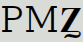
\includegraphics[width=0.20\linewidth]{chast-colebanie-osnov/letyaz/pmz.png}
\end{center} 

Последняя буква – «земля», «з». Ученые берут и толкуют – это не буквы, а руны. «M» – две отдельные руны, а «земля» тоже руна, но без вертикальной палочки. И надпись надо читать: «kut». Засучив рукава, толкователи рун берутся за дело. Одни говорят, что «kut» – окончание имени некоего скандинава! В высшей степени научно. Другие бают – а вот давайте добавим еще букву «r», да поменяем звуки, получится gótr или gautr, что можно было бы перевести как «мужчина» или «воин». Третьи утверждают, что тогда «Gautr» это другое имя бога Одина. Четвертые не согласны, и видят в надписи другие руны – слово «góts», но это если вторая руна длинное – «ó», а последняя – «s».

Итак, ясно вычерченную на монете славянскую надпись ученая братия считает «норманскими» рунами, толком не понимая, какие же именно руны написаны, и предлагает уйму вариантов прочтения.

Вместо того, чтобы задуматься о прочтении письмен старославянских...

Ведь как читали? Разложим вопрос на две части. Способ и произношение.

Способ. 

Как читает грамотный современный человек? Он читает не по буквам, а по словам, зная как они выглядят. Слова для него – картинки. Лишь новое слово постигается вначале побуквенно, что нужно, дабы знать как произносить слово, а потом оно становится цельным изображением. Чтобы различать слова, человек пользуется, упрощенно говоря, пробелами между ними. Это позволяет быстро понять, где начало слова, где конец, а всё что между этим – изображение слова.

В рукописях на старославянском, будь то летописи или религиозные сочинения, слова никак не разделяются, буквы идут сплошными рядами. Это относится и к греческим рукописям, а хоть бы и Нового Завета.

В лучшем случае старославянский писец ставил точки (посередине высоты строки), разделяя логически части предложения, дабы облегчить чтение. При таком положении дел вы не можете быстро найти нужный вам отрывок, не можете постигать написанное пословно, просто глядя на абзац или предложение. Вам нужно читать побуквенно и, дабы не сбиться, водить пальцем  по строкам, будто палец – это курсор. Итак, чтение было не пословное, а побуквенное, и только прочитанная порция букв могла быть сложена в слово, а затем чтец начинал читать следующие буквы, покуда не натыкался на конец слова, если конечно знал его. В случае согласной в завершении слова ставился твердый знак, что указывало на конец слова.

Произношение. Никто не ведает, как говорили на латыни во время, когда ею пользовались в обиходе. Никто не в курсе, как говорили на старославянском. Как вслух читались слова, которые написаны в летописях. Современное духовенство может читать на «церковнославянском», но это осовремененный выговор, приближенный к русскому языку последних нескольких веков.

Как же восстановить произношение времен, например, Нестора Летописца?

Сохранились переводы на старославянский с того же греческого, и перебрасывая мостки между греческим произношением (хотя никто не знает, как тогда произносили написанные слова Греки), можем примерно догадаться о разных вещах.

Буква «Є» – называемая в церковнославянском «есть». В старославянских текстах не встречается привычная нам «Е», но есть такая «Є», как в украинском, где этот знак обозначает как раз русское «е» – «йэ».

Однако, в старославянском, и дореволюционном правописании русского языка, была буква Ѣ (ять).

Очевидно, что держать две буквы для использования одного и того же звука не было нужды, следовательно буквы «Є» и «Ѣ» звучали по-разному. Кстати, до революции использование слов с «Ѣ» просто держали в памяти, толковых правил этому так и не вывели. 

Самоназвание жителей Греции  – Эллины. В летописях оно пишется как «Єллини». Думаю, прежнее произношение буквы «Є» соответствует современному «Э». Не зря она даже пишется как повернутая в другую сторону «Є». В старославянских переводах имен тех же ромейских императоров, пишется «Є», хотя звучали они с современным звуком «Э». Вывод напрашивается сам собой.

«И» (церковнославянская «иже») – и парная ей «І», она же «Ї» (называется «и»). Опять же, было отличие в произношении, как в случае с «Є» и «Ѣ». Вероятно, «И» была более «толстой», ближе к «ы». На ум приходят всё те же летописные «Єллини».

«Г» – я не знаю, отколь повелась твердая «г» почти как «к». Но вот даже во времена Петра I писали «г», а говорили «х». Это проявляется в письменных ошибках Петра I, который писал как говорил – ВыборХ, ПетербурХ. Это объясняет написание имени Юрия Долгорукого в некоторых списках в виде Гюрги, что звучит непривычно жестко на современное произношение, но если читать смягченно, выходит Хюрхи, Юрий.

Лишнее подтверждение былой мягкости «г» – использование ее в передаче иностранных имен и названий, которые в подлиннике звучат с «х» – Гамбург (Humburg), Герберт (Herbert), Гарри (Harry) и так далее. Такое написание могло обоснованно возникнуть лишь во время, когда «г» звучала столько мягко, как соответствующая ей латинская «h». Вспомним, как в старину вместо «история» (history) писали «гиштория», или не испанский, но «гишпанский».

«Оу» – еще одна любопытная штука, сочетание букв, позже перешедшее в обычное «у». Например, «Златооустецъ», «моужъ». Вместе с тем, встречается и одиночное «у» – «служебнии». Поскольку письменный язык отражал устный, значит, некоторые слова так и произносились, и вместо короткого «муж» растягивали «моуж». Сие возможно при довольно неторопливой речи, надо успеть произнести. Потом, с течением лет, веков, речь наверное ускорилась, и «лишнее», трудное произношение отпало в пользу короткого. И коротко превратилось в кратко. Выпадали даже целые слова – «еси» – а у англичан оно сохранилось как «is». Сравните Сие еси и this is. 

Медленная устная речь хорошо согласуется с медленным же чтением сплошных рядов букв. А что, если и мысли в то время протекали медленно? 

%Выдумка заменяет ученым обоснование и в решении других вопросов.

\chapter{А так говорят грамоты}

Век двадцать первый, государство Литва, расположено на южном побережье Балтийского моря. Столица Литвы – город Вильнюс. Официальный язык – литовский, относимый к балтийской группе. Состоит из двух говоров – жемайтского и аукштайтского.

Века давние, Великое княжество Литовское, включает в себя земли нынешней Литвы, Беларуси, Украины. Столица княжества – город Вильнэ, Вильна, что буквально значит «вольная». Официальный язык – «руский» (с одной «с»), как он назван в тогдашних документах.

Земли государства, которое мы привыкли называть Киевской Русью, после ослабления в княжеских распрях, попали в зависимость к Орде. Затем, в 14-16 веках, вошли в состав Великого княжества Литовского, позже – Речи Посполитой.

Тартары были изгнаны из Киевской Руси в 1320 году объединенным воинством Русов и литовского князя Гедимина. Несколько позже Литовское княжество посредством браков соединилось с меньшим по размеру Королевством Польским. Влияние Польши постоянно увеличивалось, покуда в 1569 году Литва и Польша не срослись в то, что ныне именуют Речью Посполитой.

Документы – кровь государства. Оборот документов – циркуляция крови в его организме. Осталось множество, а еще больше утрачено, бумаг того времени – приказы, купчие, жалованные грамоты, законы. Писались они на нескольких языках – на латыни, польском, а во время сильного княжества Литовского – на «руском», с одной «с».

Об этом руском языке теперь много спорят. Белорусские историки величают его «старобелорусским», украинские – «староукраинским» или «древнерусским», россияне – то «северо-русским» и «западно-русским». Одни ученые доказывают, что это был чисто письменный язык, другие указывают на второе его имя – «проста мова», то есть народный, обиходный язык, третьи возражают, будто литовские князья не могли на нем говорить, а общались на другом, «балтийской группы».

Язык общения князей оставим в стороне. На руском, в Великом княжестве Литовском – в Вильне и в Киеве – составлялись завещания, писались протоколы, велись учетные книги, подавались жалобы. Огромный объем документов, известных как Литовская Метрика – по сути, архив канцелярии Великого княжества Литовского – написан большей частью на руском.

На нем был создан в 16 веке и свод законов княжества, Литовский статут, переведенный затем на польский. Однако статут и юридическая терминология Литвы вобрала много польской, а Поляки пользовались в юриспруденции латинскими выражениями, поэтому литовский «юридический» язык это такой сплав славянского и ополяченной латыни, причем чем дальше, тем больше.

Польские чиновники, с усилением влияния Польши, противодействовали использованию руского языка как официального, ибо понимали его всё хуже. Они хотели документов на польском или латыни, и хотя поначалу от этих нападок на язык удавалось отбиваться указанием на традицию – «листы писаные и выдаваны руским писмом и языком по всему панству его королевской милости великому князству литовскому», на Варшавском сейме 1696 года «руска мова» утратила статус официальной.

Неясно, в какой мере этот руский язык Литовского княжества соответствовал разговорному народному языку – говорам Литвы, Белоруси и Украины – поскольку мы имеем дело с письменными документами. Ведь если судить по польским латинским документам, то истолковывая это как прямое указание на язык народный, следует заключить, что Поляки поголовно говорили на латыни. Очевидно однако, что руским языком в княжестве Литовском пользовались и знали его хорошо.

Давайте ощутим вкус этого языка, тем более что далее в книге мы будем часто встречаться с источниками на нем. Пример из свода законов – Литовского статута, писано от имени великого князя\footnote{Здесь и далее для удобства чтения документов княжества Литовского буду отбрасывать твердые знаки, что ставились после согласных в конце слов (как в царской России), а порой и внутри. Также заменяю «і» на «и», а в письме московского князя, «іа» на «я»}:

\begin{quotation}
21. Хто бы новые мыта уставлял.

Тэж приказуем, абы жадин чоловек в панстве нашом – Великом князьстве Литовском – не смел новых мыт вымышляти ани вставлять ни на дорогах, ани на местех, ани на мостех, и на греблех, и на водах, ни на торгох в именьях своих, кром которые были з стародавна вставленые, а мели бы на то листы продков наших, великих князей, або наши. [...]
\end{quotation}

Этим приказываем, чтобы ни один человек во владениях наших – Великом княжестве Литовском – не смел новых мыт (пошлин) измышлять и устанавливать ни на дорогах, ни в городах, ни на мостах, ни на греблях (плотинах), ни на водах, ни на торгах (рынках) в имениях своих, кроме тех мыт, которые были издавна установлены, и подтверждены листами (документами) предков наших, великих князей, либо нашими листами.

Вполне понятный славянский язык. И это писалось вполне славянскими буквами, что зовутся кириллицей, а числа употреблялись тоже буквенные, как в «старославянском». Многое в этом языке было как в «старославянском» – слова с согласными на конце завершались твердым знаком, те окончания, где мы пишем «ях», здесь и в старославянском – «ех», то бишь «на санех» вместо «на санях». Однако видим и развитие письменное, если сравнивать с летописями – слова разделяются пробелами, хотя нет еще запятых, а точек мало. Но ведь летописи старше! Язык их старше! Я усматриваю в языке литовских документов развитие того же языка, который прежде был запечатлен в летописях.

Однако, это не просто развитие с течением времени, но развитие, испытавшее влияние местных говоров, ведь славяне и ныне в разных местах говорят с отличиями даже в пределах одной страны.

Еще один пример – выдержка из договорной грамоты Литовских князей Евнутия, Кестутия и Люберта Гедиминовичей, Юрия Наримундовича и Юрия Кориатовича, с Польским королем Казимиром, с Мазовецкими князьями Семовитом и братом его Казимиром, сыновьями Тройдена. Дата неизвестна – но после 1340 года. Итак, межгосударственный договор правителей. Я буду последовательно излагать его и толковать с руского на русский:

\begin{quotation}
Ведаи то каждый человек, кто на тый лист посмотрит. Оже и князь юунутий, и кистютий, и любарт, юрий наримонтович, юрий кормиантович.

чинимы мир твердый. ис королем казимиром польским. и сомовитом и с братом казимиром мазовскым, и с его землми, краковьскою и судомирскою, сирязьсклю, кумвьскою, лучичскою, добрыньскою, плотьскою. мазовскою, люблинскою, сетеховьскою, и со львовскою.

а за великого князя олькерта и за кориата и за патрикиа, и за их сыны, мы ислюбем, тот мир держати велми твердо, безо всякое хитрости.
\end{quotation}

Доводится до сведения каждого, кто на этот документ посмотрит. Далее перечисляются участники договора. Утверждаем мир твёрдый, с такими-то, и подвластными ему землями сякими-то. Мир держать очень твердо, без всякой хитрости.

\begin{quotation}
не заимати нам королевы земли, ни его людий што его слухають, королевы держати львовскую землю исполна, а нам держати володимерскую, луцкую, белзьмкую, холмьскую, берестинскую, исполна жь.
\end{quotation}

Не захватывать нам (литовским князьям) земли польского короля, ни его подданных. Королю – целиком владеть львовской землей, а нам – володимерской, луцкой и прочими, тоже полностью.

\begin{quotation}
а мир о покрова богородицы до ивана дне до копал, а о ивана дне за 2 лет,
\end{quotation}

Мир заключается от праздника Покрова Богородицы до Иванова дня, а после него два года.

\begin{quotation}
а городов оу руской земли новых не ставити, ни сожьженого не рубити, доколя мир стоит, за 2 лет, а креманец держати юрью наримоньтовичю от князий литовскых, и от короля, за 2 лет. а города не рубити. а коли мир станет, юрью князю города лишитися.
\end{quotation}

Пока держится мировое соглашение, два года, в руской земле нельзя ставить новых городов (крепостей), и сожженных не восстанавливать. Креманец два года держать совместно Юрию Наримонтовичу от литовской стороны, и от короля. А по завершении мирового соглашения, князь Юрий лишается права на «держание» города Креманца.

\begin{quotation}
аже пойдет оугорьскый король на литву, польскому королеви помагати, аже пойдет на русь што литвы слушает, королеви не помагати.
\end{quotation}

Если пойдет угорский (венгерский) король на Литву, польский король должен помогать Литве. Но если угорский король пойдет на Русь, подчиненную Литве, то польский король не должен вмешиваться.

\begin{quotation}
а поидет ли царь на ляхи, а любо князи темний, князем литовьским помагати.
\end{quotation}

Если нападет царь («а любо князи темний» – либо темный князь) на поляков, литовские князья должны помогать полякам.

\begin{quotation}
аже пойдут на русь што короля слушает, литовьским князем не помагати.
\end{quotation}

Но если нападут на Русь, подчиненную польскому королю, литовские князья не помогают Польше.

\begin{quotation}
а про любарство ятство, хочем его поставити на суде перед паны оугорьскими, по сошествии святого духа за 2 недели, литовским князем стати оу холме. а королеви оу сточьце, кде смолвять тут будет суд,\end{quotation}

А вопрос про держании в заложниках Любарта (он же Люберт, сын Гедимина) хотим поставить на суде перед правителями угорскими, через две недели после праздника Сошествия Святого Духа. Литовским князьям стать на холме, а польскому королю в «сточьце», где договорятся там и состоится суд.

\begin{quotation}
тягатися ис королем. будет ли ял его король по кривде, любарт будет прав, и я князь кистютий буду прав перед вгорьскимь королем, будет ли король прав, нам своего брата любарта дати оугорьскому королеи оу ятьство.
\end{quotation}

Короче говоря, если правда на стороне польского короля, Любарт пойдет заложником к угорскому королю.

\begin{quotation}
а коли будет по миру, кто не оусхочеть далей миру держати, тот отповесть, а по отповеденьи стояти миру за месяц.
\end{quotation}

Если во время перемирия, кто-либо не захочет его далее придерживаться, то должен уведомить об этом, и после уведомления соблюдать мир еще месяц.

\begin{quotation}
аже пойдут татарове на львовскую землю, тогда руси на львовьце не помагати. аже пойдуть татарове на ляхе, тогда руси неволя пойти и с татары.
\end{quotation}

Если пойдут Татары на львовскую землю, Русь не должна помогать львовцам. Если пойдут Татары на Поляков, Руси нельзя присоединиться к Татарам.

\begin{quotation}
а оу том перемирьи кто кому криво оучинить, надобе ся оупоминати старейшему, и оучинити тому и .. (пропуск) праву, оучинить которыи добрый человек кривду, любо воевода, а любо пан, оучинити исправу из ним.
\end{quotation}

Если в том перемирии кто кому обиду нанесет – надо его имя назвать старейшему, и вынести ему приговор по закону. Далее уточняется, что «старейший» это воевода либо «пан», словом начальство. 

\begin{quotation}
аж сам не может заплатитить тот истиньный. што же оуложат его оу вину, хочет ли сам король заплатити на нь, а его дедичество себе оузяти.
\end{quotation}

Если осужденный не в состоянии заплатить положенное приговором, то король может заплатить вместо него, а наследное имущество приговоренного взять себе.

\begin{quotation}
не оусхочет ли король сам заплатити, даст тому то дедичество, кто его потяжет.
\end{quotation}

Ежели король не хочет сам заплатить, то отдаст имущество ответчика истцу.

\begin{quotation}
а за избега можем его добыти и выдати. аже его не можем добыти, можем его искати с собою сторону. аже побегнет русин а любо руска, или во львов, или холоп чии, или роба, выдать его.
\end{quotation}

А за уклонение, побег, можем его (ответчика) поймать и выдать. Если не можем его поймать, будем искать. Если бежать будет русин (или руский – а любо руска), или во Львов, или же убежит холоп чей или раб, следует его выдать (вернуть).

\begin{quotation}
а што в тои грамоте писано, тую ж правду литовьскым князем держати. а на то есмы дали свои печати.
\end{quotation}

Что в этой грамоте записано, так закон соблюдать литовским князьям, и это подтверждаем своими печатями.

Но одни народы и языки взяли верх над другими, город Вильна стал Вильнюсом. А еще в 16 веке, когда Вильнюс был Вильной, король Жикгимонт (Сигизмунд) выносит приговор по спору городничего виленского Урлиха Гоза с Яновой Катериной. Вот документ, сохранившийся в Литовской метрике. Это подлинник:

\begin{quotation}
Вырок Улриху Гозу, городничому виленскому, з мещанкою виленскою Яновою Катериною о част дому на Немецкои улицы, куплю его у матки ее.

Жикгимонт

Смотрели есмо того дела.

Стояли перед нами очывисто, жаловал нам городничыи виленскии, минцар наш, пан Улрих Гоз на мешчанку виленскую Яновую Катерыну в том, штож деи он купил в матьке ее часть дому ее в месте н(а)шом Виленском на Немецкои улицы, и мы часть того дому потвердили ему н(а)шым прывилем водле купли его, и на то он прывилеи наш перед нами вказывал. А тая деи Катерына тую част в мене отняла и держыть оть колка леть, нет ведома которым обычаем. И тая Катерына перед нами мовила, иж она тому не сведома, которым обычаем он то купил.

Ино мы городничого пры том потвержени н(а)шом зоставили, нижли маеть он лист купчыи на часть того дому положыти на ратушы перед воитом и бурмистром, и радцы места Виленского. А воить з бурмистры и радцы мають то межы ними розознати подле части купли его, и водле права их маитбарского.

Псан у Вилни, под лет Бож нарож 1000 пятсот 22 мсца нояб 29\footnote{29 ноября 1522 года.}. Индик 11.
\end{quotation}

Городничий Урлих Гоз купил у матери мещанки Катерины Яновой часть дома на Немецкой улице, и Жикгимонт подтвердил сделку привелеем, предъявленным позже Гозом. Но Катерина ту часть дома у Гоза отняла и непонятно по какому праву (закону) удерживает несколько лет. Жикгимонту же она говорит, что «иж она тому не сведома, которым обычаем он то купил» – не знает, каким образом Гоз ту часть дома приобрел. Решение таково – если городничий имеет купчую на часть того дома, пусть предъявит ее в ратуше войту и бурмистру, и радцам (советникам) Вильны. А войт с бурмистром и радцами пусть между собой определятся по части законности купли, согласно их магдебургскому праву.

Хорошо, а на каком языке литовские чиновники обращались к чиновникам польским? Снова приведу документ из Литовской Метрики, за 12 октября 1553 года. Не буду уже заниматься его толкованием, просто хочу показать – тот же руский язык, только влияние польского усилилось. Руководство переписчикам польским, со стороны княжества Литовского, об учете скота, выпасаемого на полях королевскими (цесарскими) подданными:

\begin{quotation}
Наука писаром польским, з стороны Великого Князства Литовского пану Венцыславу, секретару, а стороны Коруны Польское пану Станиславу Вороневскому, яко ся мають справовати около пописаванья быдля которое на полях короля его милости подданые цесарские паствити будуть.

Напервеи ожидати того будуть абы сандчак белогородскийи пану воеводе бельзскому, князю воеводе киевскому отказ вчунил на тые листы которие з росказанья короля его милости до него писаны будуть, ознаймуючи ему о постановенье около тых поль межи королем. его милоцтью а цесаром турецким 

А кгды ознаимить, же вжо росказал росказаньем цесарским подданим абы без оповеданья и постанобенья дани от пашни на поля короля его милости не ездили, поедут до Белагорода и там становенье около тое пашни чинити мают старючи ся о то пильне, абы вси тые каторые паствити на полях короля его милости будут, списаными мели, и много которих стад як великих мети будут. А то все списабши до его королевское милости прислати мають.

Там же теж вже и умову вчинят, по чому от ста волов, конеи и овец платити мают абы о то при выбиранью дани трудност не была.

Будет теж того пильне догледати, жебы от подданых короля его милости шкоды жадные не делали ся тым которие умовы о паству вчинят. А которого бы такового дознали, жебы шкоды чинити мел мает его королебская милост писаным своим ознаимити стороста его милоцти бапскоми у браславскомы опобедати

А того напильнеи стеречи маете, абы во всемт згодлыве тую послугу короля его милости оправили пожитку и скарбу его королевское милости стеречи мают 

А остатокь корол его милостцноте и вере их поричити рачит.

Писан у Ломзе лет Бож нарож 1553, мсца ок 12 дня.
\end{quotation}

А вот каков язык письма московского князя Василия III к Жикгимонту в 1526 году, выдержка:

\begin{quotation}
Лист кнзя великого московского перемирныи до шести лет с королем его млстю Жикгимонтом\\

Мы, великии гсдр Василеи, Божею млстью гсдр всея Руси и великии кнзь володимерскии, новгородскии, псковскии, резаньскии, тферскии, югорскии, пермскии, болгарскии и иных. Что прысылал до нас тот брат нш, великии гсдр Жыкгимонт, Бжею млстью корол полскии, великии кнзь литовскии, рускии, кнжа пруское и жомоитскии, и мазовецкии и иных, послов своих, воеводу полоцького, старосту дорогицкого, пна Петра Станиславовича, а подскарбего земского, маршалка своего, старосту слонимского и каменецкого, пана Бгуша Бговитиновича, о миру и о доброй смолве. 

И то межы нас с тобою, братом нашым, з великим гдрем, з Жыкгимонтом, королем и великим кнзем, нне не стало ся. И послы твои, брата ншого, говорыли нам от тебе, брата ншого, от великого гсдря Жыкгимонта, короля полского и великого кнзя литовского и руского, чтобы мы взяли с тобою перемире на шест лет на то, чтобы нам в те перемирные лета межы собя рати и войны не замышляти, а слати нам в тых летах межы собя на обе стороны своих великих послов, которые межы нас то дело могуть делати. [...]

А в те перемирные лета какова учынитца обида меж ншых кнзеи в землях и в водах, и в ыных каких обидных делех, и ншы кнзи и наместьники, и волостели украинныи сослався, да тем обедным делом всим управу учынят на обе сторо­ны. А в каких обидных делех нашы кнзи и наместьники, и волостели не учынят управы и нам о том сослати судеи. И они съехався да тем обедным делом всим управу учынять на обестороне стороны без хитрости.

А татя, беглеца, холопа, робу, должника по исправе выдати; а даное, положоное, заемное, поручное отдати. [...]
\end{quotation}

\newpage

Я усматриваю две ветви развития «летописного», старославянского языка – западную и восточную. Как видим, обе они уже отличались от языка летописей, но поначалу сохраняли большое сходство. Одновременно продолжал использоваться, для церковных нужд, и устаревающий «старославянский», всё более отдаляясь от разговорного народного и светского письменного.

На каком языке говорили в Киеве, допустим, в 15 или 17 веке? На языке, отраженном в документах того времени? Или население, используя разные устные говоры (в Киеве обитали сообщества разных народов), в письменном мире пользовалось общим для княжества Литовского, руским языком? Который кстати не имел четких правил. Можно найти отличия в документах в зависимости от местности. Так или иначе, этот язык понимали даже на межгосударственном уровне. Сохранялась еще общность Славян, и язык общий еще не разделялся на ветви столь существенно, как ныне. Присущие разным славянским землям говоры были более схожи между собой, чем, например, современные русский, украинский и белорусский. 

Знакомясь с историей Киева, мы встретимся и с языком летописей, и руским (с одной «с») языком документов времени Великого княжества Литовского. 

Я не раз сталкивался в книгах с подходом, когда ученый цитату из источника приводит в подтверждение своих слов. Постараюсь действовать иначе, источник делая основой рассуждений. Поэтому разбор какого-нибудь источника порой затянется на множество страниц, ну да мне важно не подтвердить свою мысль, а докопаться до сути. Сначала надо точно выяснить, что хотел сказать например летописец, а уж затем толковать  сказанное им. Смысл слов со временем меняется, надобно всегда возвращаться туда, где и когда они сказаны, и кем сказаны, чтобы понять, о чем идет речь.

\chapter{Потоп}

В каком-то сборнике баек про якутских шаманов мне попался рассказ, как шаман рожал через пупок. Верить этому или нет?

Ученые говорят, что был ледниковый период, даже несколько, и во время последнего жили мамонты и дикие люди, охотники на мамонтов. О том, что случилось такое оледенение, геологи судят по следам и показывают их нам. Это различные пески, глины, галька, щебень. Другим следам учеными придуманы названия особые – ледниковая муть, котлы, бараньи лбы.

Правда, в зависимости от научной школы, геологическое строение одного и того же холма может трактоваться по-разному. Например, холмы Киева покрыты суглинком особого рода – наука именует его лёссом\footnote{Немецкое слово «löss» в 19 веке ввели ученые, для обозначения суглинков с определенными составом и строением. У нас его называли желтозёмом, белоглазкой да просто суглинком. Но геологам оказалось мало понятных русских слов, стали пользоваться невразумительным «лёссом», еще и заменили «ё» на «е», получив уродливое подобие нашего «леса». Поди разбери! Слово это глубоко уже въелось в околонаучный язык, я же по возможности буду стараться писать «суглинок».}. Насчет происхождения лёсса существует множество предположений. Кроме прочего, одни говорят, что образовался он от ледника. А другие – лёсс надуло ветром. Обе точки зрения имеют доказательства. И сторонники ледникового лёсса говорят – был такой скандинаво-русский ледник, покрывал земли от Скандинавии до Полтавщины\footnote{По науке, Скандинавия – главный благодетель славянских земель. Дарит им то ледники, то князей.}. Украина вообще богата лёссом, что лежит под черноземом степей да под холмами. Подойдите в Киеве к любому котловану или раскопу на улице, поглядите на слои почвы. Темной земли сверху совсем мало, а ниже идет бурый или светлый суглинок. Обрывистые кручи над Днепром тоже лишь слегонца покрыты землей, под нею – суглинок.

Ледник вёл себя как-то странно. По словам геологов, он то отступал, то снова наступал, подобно обычным волнам, хотя на деле увеличивался либо уменьшался. Ученые разделяют эти приливы и отливы тысячами лет. Ведь принято считать, что природа меняется медленно.

А если вместо ледника были и в самом деле волны? Ведь то, что нам показывают как следы ледника – пески, гальки и прочее – мог принести не ледник, а наводнение. Огромное. Всемирный потоп.

В преданиях, пожалуй, всего мира есть упоминания о великом Потопе. Отражен и в Библии, и в устных рассказах уральских Манси. Приведу несколько мансийских преданий\cite{perevalova01}:

\begin{quotation}
За семь лет до начала потопа шаманам стало известно о приближающемся времени огня и воды. Шаманы били в бубны, гадая о том, как можно спастись. Люди, не умевшие плавать, стали строить плоты (пор). Только семислойный плот (лабыт лаур полет пор), сделанный из семи бревен в семь слоев, покрытый семислойным пологом из кож осетра и стерляди, мог устоять против стихии. 

В какой-то местности, выше Березова, росла священная береза с семью отростками от вершины. Однажды береза та упала и из под ее корней начала бить вода. Люди укрепляли это место, но никак не могли остановить водяного потока. Тогда люди расселись на плоты, и их понесло вниз течением Оби. Женщин и девушек на плоты не брали, их все равно вода с огнем сжирала, спасались только мужчины и «чистые» девочки. 

Семь дней вода кипела – огонь и вода вместе шли. Нижние слои плотов разбивались, верхние слои пологов сносило. Вместе с огненной водой несло множество огромных ящеров\footnote{Отметим кстати болота земли Уральской и многочисленные древние фигурки динозавров, находимые в тех краях.} и змей, которые взбирались на плоты и поедали людей. 

Много народу тогда погибло – те, кто не успел построить семислойного плота, те, кого смыло водой. Когда стихия улеглась, люди стали высаживаться на высоких островках – пугорах. Приплывших на плотах людей называли нобтын ёх – «приплывший народ» или пор ёх – «люди плотов».

[А.П.Кондин, п. Казым-мыс, р. Б.Обь, 1990].
\end{quotation}

Вот еще:

\begin{quotation}
Вода была везде, кроме Урала. Когда вода прибывала, на высоких склонах Урала собирались и люди, и животные – медведи, волки, лисы, росомахи. Целую неделю бушевала вода. Люди и животные вместе жили, и никто никого не боялся. На этой горе собрались разных родов и даже народов люди. После спада воды люди разошлись по разным юртам и стали жить родами. Один зырянин пришел из-за Урала (Нерапса ху) и во время потопа оказался с хантами на одной горе, после чего породнился с ними.

[Т.И.Хунзи (Озелова), п. Унтсыльгорт, р. М.Обь, 1989].
\end{quotation}

У Греков, при помощи Потопа, Зевс уничтожает людей, ставших ему невыносимыми. Помогают в этом Посейдон и владыка ветров Эол. Спасается на плоту лишь сын Прометея, Девкалион с женой своей Пиррой. Они, проплавав 9 дней по безбрежью, пристают к оставшейся над поверхностью воды вершиной Парнаса. «Девкалионов потоп» служит как бы основой, отправной точкой человеческой истории Греции. В греческих преданиях есть сведения и о других потопах, либо том же, но с иными действующими лицами, коим выпадает счастье выжить – например, это Дарданус, сын Зевса и Электры.

У Индусов\footnote{Подробности читайте в «Матсья Пурана», «Бхагавата Пурана» и «Махабхарата».}, бог Вишну через своего аватара Матсью предупреждает о потопе человека, правителя Дравиды (южная часть Индии) йога по имени Ману, и советует строить большой корабль, куда взять, условно говоря, всякой твари по паре, чтобы затем населить землю заново. По индийским преданиям, все люди после потопа произошли от этого Ману, в то время как христиане выводят род человеческий от уцелевшего Ноя.

О потопе людей предупреждают то шаманы, то боги. Значит, более осведомленные знали о надвигающейся беде заранее, и некоторых она не застала врасплох. Люди пытались спасаться на возвышенностях. Потом, надо думать, вода спадала, где быстрее, где медленнее. В главе про Киевское море мы еще обратимся к сведениям об якорях и обломках морских судов, находимых в степях Левобережья.

Вообще в моей книге время от времени я буду касаться Всемирного Потопа, как одного из событий прошлого, события, которое оказало влияние на формирование рельефа и на развитие наземной жизни. Но прежде чем двигаться к другой теме, порассуждаю еще.

Докучаевский переулок в Киеве. Прорезался оврагом к огромному Протасову яру от расположенной выше, чем проулок, Докучаевской улицы. Назван в честь Василия Докучаева, геолога и почвоведа. Научные работы Докучаева очень интересно читать, они написаны живым языком, Докучаев приводит взгляды, противоположные своему, и оспаривает их.

В его книге «Способы образования речных долин европейской России» речь неоднократно  заходит о мамонтах и шерстистых носорогах. Приведу пример, впрочем без иллюстрации – не могу снова найти в закромах книжку. Место этого обрывистого берега речки Качни, по описанию Докучаева

\begin{quotation}
находится на левом берегу речки, близ устья Гридневского ручья. Как видно, в нем можно различать следующие слои\footnote{Описываются сверху вниз.}:

A, высотой 6 футов (30,48*6/100 = 1.82 метра). Обыкновенная бледнокрасная, рыхлая, песчаная глина без галек и органических остатков; кверху она постепенно переходит в растительный слой,а книзу в ней заметно все более и более преобладание песку. 

B, высотой 4 фута (30,48*4/100 = 1.21 метра). Верхние три фута состояли из беспрестанно перемежающихся прослойков темной глины с пропластками песку, то желтого, то очень красного, то мелкого, то довольно крупного (гравий); 

слои постоянно выклинивались или незаметно переходили один в другой, на расстоянии нескольких десятков шагов вдоль берега; слои были так мелки, что их в 3 футах насчитывалось до 25 и более; только при самом основании этого пласта виднелся совершенно однородный, чистый, светло-красный песок с фут толщиной. Весь слой был переполнен древесными стволами, которые лежали обыкновенно горизонтально и были лишены в данном разрезе мелких сучьев. 

На самой границе с пластом С были найдены мною части ступни, атлант и несколько ребер мамонта и зуб, принадлежавший тому же животному (Elephas primigenius), кроме того, здесь же попадались еще, хотя и не особенно обильные, мелкие, совершенно уже сгнившие остатки каких-то других костей.

С, высота половина фута - около 15 сантиметров. При самом основании обрыва, подымаясь над уровнем реки едва на 1/2 фута, выступала грязно-синяя вязкая глина, но ее можно было проследить на несколько фут. под водой, откуда торчали иногда громадные древесные стволы. Замечательно, что местные крестьяне именно из этого пласта выкапывают наиболее сохранившиеся дубы, которые они и употребляют на различного рода поделки; они даже заверяли меня, что некоторые экземпляры были здоровее - плотнее ныне живущего дуба; в этом случае, вероятно, уже началось окаменение дерева 
\end{quotation}

Итак, три слоя - три горизонта. Образование верхнего, медленное, постепенное, Докучаев объяснял так:

\begin{quotation}
Благодаря тому обстоятельству, что этот пласт всюду образовался частью из отложений весенних вод, а частью - на счет мути, приносимой с соседних высот атмосферными водами, минеральный состав его, понятно, не мог быть строго определенный: это есть смесь в различных пропорциях тех горных пород, которые встречаются в бассейне данной реки;\end{quotation}

Этот верхний пласт – лёссовый. Вот Докучаев выразил одну из причин его возникновения – намыло, нанесло водой. Отложения весенних вод и наносная муть с соседних высот.

   Ага, получается, соседние высоты сами состоят из суглинка. Как же он образовался там? А там надуло ветром? 

   Что же, слой суглинка высотой 1.82 метра, под ним слой 1.21 метра, с костями мамонта и лежащими стволами деревьев. Рассуждая логически, мы придем к выводу, что кости мамонта были покрыты слоем суглинка в 1.82 метра.

   Река Качня, ныне Касня, в Смоленской области, течет по равнине. Не знаю, каковы были – и были ли – паводки на ней до устроения там водохранилища. Докучаев уделил ей отдельную работу, «О наносных образованиях уезда Смоленской губернии».

   Но исходя из геологического разреза, приведенного Докучаевым, мы должны предположить, что для образования над современным Докучаеву уровнем воды в речке, должны быть справедливы следующие положения.

   Уровень воды в реке время от времени повышался и намывал этот суглинный слой, сначала покрыв упавшие почему-то кучей деревья, покрыв останки мамонтов, а потом уже шел намыв на ранее намытую муть. 

   Уровень воды в небольшой реке должен был повыситься, однако, в сумме почти на 4 метра. И вот странно. Постепенно намываемый суглинный берег не зарастал новыми деревьями, кустами... Нет, он, получается, долгое время ждал, и лишь потом соизволил покрыться сверху слоем более-менее плодородным.

   Переулок Докучаевский, Протасов яр. Яр этот прор\'езал Батыеву и Байкову горы и спускается от района Соломенки к речке Лыбедь. Перепад высот – около 62 метра, то есть верховье яра лежит на 62 метра выше низовья. По дну яра в коллекторе протекает ручей. Сложно представить, что своим жалким течением он намыл могучие суглинные берега яра. Он их только размывал.

    А ведь в 19 веке здесь, при добыче глины для нужд кирпичного завода, тоже нашли кости мамонта. Снова закономерность – слой суглинка или глины, а под ним кости мамонта. 

Многие знают про найденного на Магадане несчастного мамонтёнка Диму. Его тело обнаружили в 1977 году на прииске имени Фрунзе, на глубине 2 метра от поверхности земли, когда бульдозером раскапывали грунт в долине ручья под названием Дима – отсюда и мамонтёнок Дима, а не от имени Дмитрий. Обычно сообщают, что нашли в вечной мерзлоте. А мамонтенок, дескать, когда-то упал в яму с водой и грязью, не смог выбраться и умер. А потом мороз заморозил тело в этом льду с грязью и так оно сохранилось до наших дней. 

   То есть, надо полагать, при падении туда мамонтёнка, вода была жидкой, но потом резко ударил мороз, заморозил ту глинистую жижу и уже не размораживался до 20 века, а к тому времени сверху опять же, намыло или надуло 2 метра некой вечной мерзлоты. Что за вечная мерзлота такая? 

   Да, кстати, про сходного мамонтёнка Любу с острова Ямал ученые тоже предполагают, что Люба задохнулась в некой в глинистой массе, а потом тело законсервировалось благодаря лактобактериям.

   Так вот про вечную мерзлоту, в которой находят мамонтят. И останки мамонтов. И поваленные деревья. Их находят не просто в какой-то почве, а в промерзшем суглинке.

   Но вернемся к киевским холмам. Много и подробно еще будем говорить о Кирилловских высотах и раскопках на них. Самые знаменитые из них - обнаруженная Викентием Хвойкой Кирилловская стоянка, от места которой поныне сохранился крутой обрыв.
    Многочисленные кости мамонтов были найдены внизу, под срытой частью горы. 
   
   По Хвойке, стоянка - а он полагал, что мамонтов убивали некие первобытные охотники и там же жили, хотя скелетов людей он не отыскал - стоянка располагалась в местности еще без гор, в полной озер котловине у большой реки, у древнего Днепра.   

Тут росли высокие кедры и ели, бродили мамонты. Но с севера, как считал Хвойка, подступал ледник, из-под которого вода несла грунт, постепенно заполняя наносами долину Днепра, пока она не переполнилась. Тогда вода выступила над уровнем долины, затапливая окрестности. Ледник надвинулся, затем начал таять, отступать к северу. Снова наносы. Река пробила себе новое русло уже в них, уровень дна снизился. Слои песка между культурными слоями, как полагал Хвойка, означают несколько затоплений местности, во время которых грунтовые наносы покрывали предшествующий культурный слой. 

   Так рассуждал Хвойка, беря на вооружение передовые для 19 века представления о леднике. Конечно, всемирный Потоп уже тогда стало модным считать сказкой. Хотя даже в рассуждениях Хвойки есть некие затопления, следами коих он считал слои песка.

   Современники возражали Хвойке –  в разрезе холма нет морены – валунной глины, которая должна присутствовать, если местность была покрыта ледником, и поэтому Кирилловской стоянке надо определить возраст не более 12 тысяч лет, когда, как считается наукой, завершился последний ледниковый период.

   Изучая потоп, вы всюду натолкнетесь на эту датировку – 12, 10 тысяч лет назад, что-то случилось. Завершился ледниковый период, случились какие-то катастрофы... Например, что вы знаете об Алтайском потопе? Ученые думают, что некие ледники создали плотину на реке Чуе, и образовалось огромное ледниковое озеро, а потом, между 12000 и 9000 годами до нашей эры, плотину прорвало и вода устремилась по Чуе в Катунь, потом в Обь и в так называемое Мансийское озеро, причем уровень воды по пути резко поднялся на 12 метров, и, дескать, этот потоп докатился даже до Черного моря.

   Следы воздействия на рельеф того, что ученые называют Алтайским потопом, хорошо видны и отражены на фотографиях и в научных работах. Однако науке проще объявить причиной потопа ледниковую плотину и ледник, нежели задуматься о всемирном потопе.

   Равно как проще объяснять места массового обнаружения останков мамонтов тем, что ледник принес суглинок и покрыл им останки. Или что мамонтёнок упал в яму с глинистой водой. Ну а большие мамонты тоже в ямы с глинистой водой падали? Нет, их убивали первобытные охотники, – пояснял археолог Хвойка. А другие археологи его спрашивали – так ведь те орудия, что вы нашли, слишком малы...

   Но главное, никто толком не объясняет, как поверх этих останков образовался слой суглинка в десятки метра высотой. Чем его нанесло?

   Оглядитесь вокруг, выйдя не природу. Вы много увидите глины? Глина почти всегда скрыта под слоем чернозема, и обнажается лишь в местах крутых обрывов, либо там, где глину добывают для производства кирпича, раскапывая склон на большую глубину. Между прочим именно так совершаются многие археологические открытия.

   Современник Докучаева, профессор Головкинский писал относительно Волги: 

\begin{quotation}
Что касается состояния страны по среднему течению Волги, то из многочисленных залежей деревьев, погребенных обширными пластами, следует заключить о хвойных лесах, покрывавших страну, все еще обитаемую мамонтом, носорогом, верблюдом и другими животными.
\end{quotation}

С чего это хвойные леса легли обширными пластами? Может их срубили и потом бросили? Нет, люди всегда рубили лес для своих нужд, потому и много лесов вырубили так, что следа не осталось. От чего же полегли хвойные леса? Почему их покрыло потом песком да суглинком? Потому и покрыло, что Потоп затопил.

   И его запомнили современники мамонтов. А от них предание через поколения дошло до нас, чтобы быть осмеянным наукой и объявленным сказкой.

   Когда вы идете по улице, и проводятся какие-то строительные работы вроде проложения труб – обратите внимание на тонкий слой чернозема сверху, и суглинок ниже. Быть может, это след Всемирного Потопа, застывшая муть, принесенная его водами и здесь осевшая.

Потоп служит одной из основных отправных точек изложения истории в летописях, хрониках, анналах и преданиях. Однако наука не верит в Потоп, при этом истово веруя в другие сведения, ею же относимые к баснословным.

\chapter{Летописание и летосчисление}

%На время не станем вспоминать, какой нынче год.

В этой книге мы будем обращаться к разным источникам – летописям, хронографам, сагам и так далее. Хронограф это вроде сборника исторических сообщений, куда выписывались сведения из летописей да иностранных хроник. Летописями же принято именовать погодичные перечни событий, относящихся к Руси.

В популярном представлении, летописи велись в монастырях, где за толстыми стенами сидели ученые монахи, из года в год записывая, что происходит вокруг и по соседству, изредка упоминая, какой заморский правитель умер или воцарился. Отчасти это так. Но летописи вобрали в себя сведения из сторонних источников, и являются сборниками. На протяжении веков они подвергались правке с разными целями.

Таковыми могли быть желание дополнить из другого источника, исправить ладность слога, исправить годы, если таковые показались ошибочными, наконец, убрать либо описать другими словами упоминания о некоторых событиях. Ведь издавна существовала цензура, как духовная, так и светская.
 
Листая страницы летописи, мы видим стройную картину. Для каждого года перечислены произошедшие события. Но когда появились в летописи эти даты? Сами ли события эти были записаны под такими годами, или много позже, при последующей правке?

Каждый, кто читает исторические сочинения древних Греков, знает – Греки, сами любители точности и ясного выражения мысли, привязывали события к правлению там-то такого-то царя. Для уточнения могли сказать – в пятый год царствования. Или – в год, когда в Олимпийских играх победил такой-то из указанной страны.

Скандинавы в сагах задают время таким же приемом. Когда там-то правил конунг такой-то, и цепляют повествование за это событие, да за события из других саг, соседних по времени и месту действия, при необходимости прибавляя – «на следующую весну», или «до осени такой-то оставался в гостях там-то, и затем отправился туда-то».

Следы подобного способа счета лет находим и в наших летописях, где не редкость привязка к византийским императорам. Правда, одни и те же события разные летописи иногда относят к разным императорам.

Возникает противоречие. Если летопись А относит крещение княгини Ольги к императору Цимисхию, а летопись Б к императору Константину, значит, в летописях А и Б – разные даты крещения. Какой летописи верить, А или Б? Отложим сей вопрос.

Сохранившиеся до наших дней, известные общественности летописи освещают события разных местностей и городов, с уклоном туда, где происходила правка и дополнение летописи. Во многих летописях первым помещается сочинение «Повесть временных лет» монаха Киевопечерской Лавры Нестора и его последователей, чье содержимое от списка к списку различно.

Самые важные летописи получили в науке названия – Ипатьевская, Лавреньтевская, Никоновская, Радзивилловская – по именам монахов, приложивших руку к их правке и составлению, а также по именам владельцев, например, патриарха Никона и Януша Радзивилла. Когда говорят «Ипатьевская летопись» и «Ипатьевский список», это одно и то же. В свою очередь, с каждого из этих списков сделаны другие списки, тоже с внесением правок.

Летописи известны читателю большей частью по редким выдержкам оттуда в книгах историков и археологов. Выдержки эти даются по изданиям, именуемым Полным Собранием Русских Летописей (знаменитое сокращение ПСРЛ), либо по другим, где наряду с подлинником дается перевод на современный русский язык.

В ПСРЛ летописи предстают перед нами в обработке учеными. Фотокопиями (светописные издания, фотолитографии) тоже издавались, в 1871 году «Повесть временных лет» из состава Ипатского списка, в 1872-м – она же из Лаврентьевской летописи, в 1875-м – Новгородская синодальная летопись, в 1880 – Ремезовская.

Отличия подлинников от обработанных вариантов таковы – нет знаков препинания, пробелы используются выборочно, все буквы одинаковой величины, числа записаны старославянскими буквами, а все буквы тоже воистину «старославянские». Ученые проделывают большой труд по приведению такого текста в удобочитаемый вид. Они меняют буквы на современные, упорядочивают слова в предложения, расставляют знаки препинания, переводят  числа в арабские. Однако, в ходе обработке возможно искажение смысла подлинника.

В известных нам летописях существует несколько основных слоев летосчисления, то есть способов считать годы от определенного опорного события. Опишу эти слои по глубине старины, от древнейшего к новейшему. Поскольку никто раньше меня о таком не писал, не грех и дать слоям имена.

Слой Царский. Это привязка к годам царствования василевсов (императоров) Византии, а также годам правления русских князей.

Слой Росписной. Ключом к пересчету лет из Царского слоя в рамки более широкого отрезка времени служит «роспись годов» – раздел летописи, где последовательно перечисляется, сколько лет прошло от библейского сотворения мира до всемирного Потопа, от Потопа до Авраама, от Авраама до «исхода» Моисея. Такими временными промежутками, или слагаемыми, летописец добирается до Александра Македонского, затем до рождения Иисуса Христа, императоров Византии, а от них к отрезкам правления князей Русских. Сложив эти промежутки, скажем, вплоть до начала княженья Вещего Олега, мы получим год начала правления Олега от сотворения мира. Число лет в каждом слагаемом бывает различно в разных летописях, поэтому слагаемые это не постоянные значения, но переменные.

Слой Годовой. Прямое указание лет, прошедших «от сотворения мира» до события, указанного в летописи. Если в Царском слое написано, скажем, «В царствование Михаила случилось то-то», в Годовом нас ждет простое: «В год такой-то случилось то-то». Казалось бы, даты Годового слоя должны быть вычислены на основе слагаемых из Росписного слоя. Это ведь Росписной слой дает нам временную основу. Однако на проверку, даты Годового слоя зачастую не совпадают с теми, которые можно получить, произведя вычисление со слагаемыми из Росписного слоя.

В летописях присутствуют все три слоя. Однако появились они в списках не одновременно, а последовательно, невесть через сколько лет, по мере необходимости, для упрощения понимания счета лет и привязки к нему событий, а может по иным причинам.

Во время, когда в летопись вводился Годовой слой, летописец, пересчитав в него из Царского слоя годы предшествующих событий, начинал записывать новые события уже в Годовом слое, отказавшись от использования Царского, то бишь опуская привязку к годам правления таких-то императоров или князей.

Сейчас человечество ведет счет лет «от нашей эры», принимая за первый ее год рождение Иисуса Христа. Так стало удобно.

Само понятие года и его составляющих (лет, месяцев, дней) зависит от особенностей календаря – его привязок к перемещению небесных светил и способу учета времени. Раньше календарей было много, да и теперь тоже. Способ считать дни – это календарь\footnote{Французы после своей революции жили по неуклюжему Республиканскому календарю 13 лет в 1792-1805 годах, и менее года в 1871-м. За начало эры считали год провозглашения республики. Недели отменили – вместо ввели «декады» по 10 дней. Но как и в семидневной неделе, выходной был только один. Введение сего календаря вызвало у некоторых небывалое воодушевление – так, в городе Аррасе устроили шествие из 12 групп по 30 человек, олицетворявших дни. Группы были построены по возрасту. В самом конце несли, под балдахином, столетнего старика – добавочный день високосного года. «Старый» новый год, 1 января, запретили. На почтах в этот день вскрывали письма и уничтожали поздравительные. Так вот, поныне даже маститые ученые совершают ошибки при переводе дат из революционного календаря в годы нашей эры. Что же говорить о переводе дат других, более древних календарей?}. А ведение счета дней, годов от определенного опорного события называется эрой.

Таким событием может быть сотворение мира по Библии, основание Рима, Хиджра (переселение пророка Мухаммеда в Медину), начало цикла древних греческих Олимпиад, и так далее.

Например, известна «эра Набонассара», которую использовал астроном Птолемей, положив началом счета лет царствование вавилонского царя Набонассара, в календарной системе Египтян. Птолемей поместил в своем астрономическом труде «Альмагест» таблицу Канон царей (Ассирии, Вавилона, Персов, Македонян, Римлян) с годами их правления, от Набонассара до Антониуса. Некоторые римские хронологи продолжили сей счет, добавляя годы правления римских императоров, по Диоклетиана включительно. После чего начали считать годы уже от Диоклетиана – наступила «эра Диоклетиана».

Каждый промежуток, слагаемое из Росписного слоя летописей – тоже, по сути, маленькая эра. 

В древности Римляне вели счет лет внутри своей эры, Египтяне – своей, Греки – своей, и так далее. Более того, почти в каждом греческом городе-государстве, полисе, действовал свой отдельный календарь. Народы жили по своим календарям и летосчислениям. И события своей истории привязывали к своим календарям и эрам.

Постепенно, народы, обратившиеся в христианство, стали приходить к общему летосчислению, что ныне мы называем «нашей эрой» или «от рождества Христова». Прежде многие тоже пользовались Годовым слоем, но считали годы от сотворения мира. И когда решали перейти на летосчисление от рождества Христова, надо было всего-то определить, в каком году «от сотворения мира» родился Христос, и потом уже вычислять год по-новому.

К примеру, выдуманный мною народ Буквоедов полагал, что Христос родился на 100-м году от сотворения мира. Стало быть, если в старинной летописи Буквоедов событие «Был неурожай капусты» подписано годом 250-м от сотворения мира, то надо от летописного года отнять год рождения Христа (тоже из расчета от сотворения мира), то бишь 250-100=150. Таким образом 250-й год от сотворения мира это 150-й год от рождества Христова, или 150-й год нашей эры.

Замечательно!

Но вот другой народ, Медоквасы, полагали, что мир был сотворен за 300 лет назад от рождения Христа. И когда в летописи Медоквасы писали «в году 250 от сотворения мира царь Горох построил город Пирогов», мы, чтобы перевести эту дату в современную, должны от 250 отнять 300. Получаем минус 50, то бишь 50-й год до рождества Христова, до нашей эры.

В пределах летописи Медоквасов всё в порядке. В пределах летописи Буквоедов – тоже. Все пишут даты от своего сотворения мира, все счастливы.

Но вот Буквоеды через несколько веков решили расширить свою летопись, да вписали в нее события из летописи Медоквасов, вместе с датами, как есть, ничего не пересчитывая. У Буквоедов в летописи теперь получается:

\begin{quotation}
Год 250. Был неурожай капусты. А у Медоквасов в царстве построен город Пирогов.
\end{quotation}

А ведь даты от сотворения мира у Медоквасов и Буквоедов разные! Но в новом варианте летописи Буквоедов это не учтено. Спустя много столетий ученые начинают переводить даты летописи Буквоедов из счисления «от сотворения мира» в «от нашей эры», или «от рождества Христова». Берут, конечно же, формулу, применимую к Буквоедам. 250-100=150. В ученых книгах появляются строки выдержки из летописи, выглядят уже так:

\begin{quotation}
Год 150 (250 от сотворения мира). Был неурожай капусты. В царстве Медоквасов построен город Пирогов.
\end{quotation}

В других ученых книгах, последующих, того короче:

\begin{quotation}
В 150 году нашей эры медоквасы построили город Пирогов.
\end{quotation}

Таким образом чисто летописно, событие построения города Пирогова было смещено во времени.

Сей упрощенный пример целиком относится ко всем летописям, хроникам, хронографам, короче говоря давним источникам. И мы скоро столкнемся с тем, что применение иной, нежели общепринятая, формулы пересчета лет – более правдоподобно. И с тем, какая путаница среди дат есть в летописях, о чем историки предпочитают молчать, используя в своих работах только общепринятые списки, но и там при вдумчивой проверке вскрываются странности.

Среди летосчислений, основанных на Библии, не было единогласия по поводу того, когда же был сотворен мир. Если сказать это другими словами – в разных эрах год рождения Христа отдален от сотворения мира на разное количество лет. Посмотрим, на какой год «от сотворения мира» приходится рождение Христа в вариантах летосчисления:\\

\noindent
Александрийская эра: 5492\\
Византийская эра: 5508-5509\\
Византийские хронисты Максим Исповедник, Феофан Исповедник и Георгий Синкелл: 5493\\
70 толковников: 5508\\
Самаритянский текст: 4700\\
Римские хронографы: 3948\\
Иудейская эра: 3761\\

%\begin{table}[h]
%\begin{tabular}{|l|l}
%\hline
%Александрийская эра & 5492\\ \hline
%Византийская эра & 5508-5509\\ \hline
%Византийские хронисты Максим Исповедник,\\ Феофан Исповедник, Георгий Синкелл & 5493\\ \hline
%70 толковников & 5508\\ \hline
%Самаритянский текст & 4700\\ \hline
%Римские хронографы & 3948\\ \hline
%Иудейская эра & 3761\\ \hline
%\end{tabular}
%\end{table}

Есть множество других.

С некоторых пор на Руси пользовались счислением, принятым в «Византийской эре». Затем, на ее 7208 году, Петр I указом ввел счисление «от рождества Христова». Так год 7208 стал годом 1700. Другие страны переходили на новую эры кто раньше, что позже.

Ученые пишут, что Византийский счет годам использовался на Руси со времени крещения князя Владимира Красна Солнышка. Подобное мнение успокаивает, придает летописным датам весомость, и облегчает пересчет летописного, от сотворения мира, года в «нашу эру», от рождества Христова.

Наука история использует для этого следующие правила.

Общее, упрощенное – от летописного года отнять 5508. Например, 6360-5508=852. Однако это правило требует некоторых уточнений.

До петровского преобразования летосчисления, было два «календарных стиля» – мартовский (пришел к нам из Рима) и сентябрьский (византийский). По первому, началом года считали март, по второму – сентябрь. Неясно, когда мартовский сменился сентябрьским. Полагают, что в конце 15 века.

Для мартовского календарного стиля правило пересчета уточняется. Если у нас есть летописная дата с указанным месяцем, и месяц этот – начиная с марта и по декабрь включительно, надо от летописного года отнять 5508. Если же месяц – январь или февраль, мы отнимаем от летописного года число 5507.

Теперь уточнение для сентябрьского календарного стиля. Ежели месяц с января по август включительно, от летописного года отнимаем 5508. Если месяц – с сентября по декабрь включительно, то отнимаем 5509.

Какие стили в каких источниках использовались? А это вечная пища для ума историков. В той же «Повести временных лет» будто есть оба стиля. Погрешность в датах, при переводе, плюс-минус один год, и так во многих древнерусских источниках.

Одним словом, формулы выработаны. Как здорово! Значит, любой год из летописи можно перевести в «нашу эру»! Но верно ли полагают ученые?

Прежде чем вести разговор дальше, я должен поведать еще об одном слое датировок. Я нарочно вынес его отдельно, чтобы не определять его положение между другими слоями.

Слой Индиктов.

Рим собирал с каждого побежденного народа дань трижды за 15 лет. На пятнадцатом году император объявлял размер дани на следующие пятнадцать лет. Латинское слово «indiction» значит «объявление», потому и год нового объявления податей назывался индиктом. Более ходовое значение слова «индикт» – просто такой-то год внутри пятнадцатилетнего цикла. Сами циклы никак не нумеровались.

В старинных источниках, в том числе наших летописях, встречаются датировки по индикту. Например, если написано, что событие случилось при Михаиле царе, в индикт 12, это значит 12-й год одной из пятнадцатилеток во время правления Михаила. Какой именно пятнадцатилетки – остается неясным.
 
Теперь, вооружившись знаниями, попробуем разобраться с датами в русских летописях и сравним наши исследования с тем, что предлагают ученые – а предложенное ими составляет основы исторической науки.

Откроем Ипатьевский список, время создания коего относят к концу 14, началу 15 веков. Издание 1871 года, подготовленный учеными текст. Летописец начинает рассказывать, в каком году, по его, летописца, источникам, стала впервые прослеживаться «Руская земля», то есть когда впервые ее упомянули. Избранная мною выдержка не случайна, в ней используются все четыре слоя летосчисления – Царский, Росписной, Годовой, Индиктов:

\begin{quotation}
В лето 6360, индикта 15, наченшю Михаилу царьствовати\footnote{Речь идет о византийском императоре Михаиле.}, нача ся прозывати Руская земля. О сем бо уведахом, яко при сем цари приходиша Русь на Царьград, яко же пишет в летописании Грецком\footnote{Об этом узнаём, поскольку при сем царе Русь приходила войной на Царьград, как сказано в летописании Византии.}; тем же и отселе почнем и числа положим:

яко от Адама до потопа лет 2242; а от потопа до Аврама лет 1082; от Аврама до исхождения Моисеева лет 430; от исхождения Моисеева до Давида лет 601; от Давида и от начала царства Соломоня до пленения Иерусалимова лет 448; от пленения до Александра\footnote{Македонского.} лет 318; от Александра до Христова Рождества лет 333; от Христова Рожьства до Костянтина лет 318; от Костянтина же до Михаила сего лет 542.

От первого лета Михаила сего до первого лета Олгова\footnote{Вещего Олега.}, Рускаго князя, лет 29; от первого лета Олгова, понележе седе в Киеве, до первого лета Игорева 31; от первого лета Игорева до перваго лета Святославля лет 33; от перваго лета Святославля до перваго лета Ярополча лет 28; Ярополк княжи лет 8; Володимер княжи лет 37. Ярослав княжи лет 40. Темьже от смерти Святославля до смерти Ярославли лет 85; от смерти Ярославли до смерти Ярополчи лет 60.
\end{quotation}

Что же? Переведем в «нашу эру», «от рождества Христова» дату 6360 «от сотворения мира» из Годового слоя так, как делает наука. От летописного года отнимаем 5508. 6360–5508=852 год нашей эры. Это число находим в учебниках, его же ученые используют в своих трудах.

Давайте проверим знаменитую формулу, по которой ученые перекладывают летописный год в нашу эру. А они говорят, что в летописи принято, будто Христос родился на 5508 году после сотворения мира.

Но вот перед нами, выше, выдержка из научного, однако не фотографического, издания списка Повести временных лет. Используя числа из его Росписного слоя, подсчитаем, сколько лет прошло от Адама до рождения Христа.\\

2242+1082+430+601+448+318+333=5454\\

5454! Простите, 5454 равно 5508? Нет. 

Так сколько лет отнять от летописного года? То, что говорят ученые, или что сказано в летописи? Разница в 54 года.

Однако проверим саму Ипатьевскую летопись печатного издания ПСРЛ. В ее Годовом слое написано, что Михаил начал царствовать в 6360 году.

По данным Росписного слоя этой же летописи, сколько лет прошло от сотворения мира до начала правления Михаила?\\

5454+318+542=6314\\

Разве 6314 равно 6360? Нет. 

Значит, закралась ошибка. Где именно? В дате Годового слоя или в слагаемых Росписного? Даты Годового слоя, кажется, должны вычисляться по числовым значениям из Росписного, и может быть, что при вычислении «года от сотворения мира» правщик летописи просто ошибся, складывая числа.

Закроем глаза на Годовой слой. 

Используя Росписной слой, вычислим, когда «нача прозывати Руская земля». Летопись привязывает это событие к началу царствования Михаила. Оно, по данным Росписного слоя, приходится на 6314 год от сотворения мира. Пересчитаем 6314 год в эру «от рождества Христова», продолжая работать с числами из Росписного слоя:\\ 

6314-5454=860 год от рождества Христова.\\

Таким образом, по Годовому слою и ученой формуле, 852 год от рождества Христова, а по данным из Росписного слоя – 860 год от рождества Христова.

Если же предположить, что число из Годового слоя 6360 всё же вернее, но год рождения Христа взять из Росписного, а не из представлений ученых, то бишь использовать 5454 вместо 5508, вычисление будет следующим:\\

6360-5454=906 год от рождества Христова.\\

Даже на таком простейшем уровне проверки летописных данных возникает путаница, и не знаешь, каким числам доверять.

Вы скажете – всего делов! Взять и поглядеть в энциклопедии, когда в Константинополе правил император Михаил! Но ведь и энциклопедическая дата – вычислена. А вычислять, как видим, можно по-разному.

Берем другой весомейший список, Лаврентьевский, в изданиях серии ПСРЛ. Он пожалуй самый древний среди известных, ибо оснащен припиской на обороте 172 листа, что списан мнихом Лаврентием в Суздали для великого князя Дмитрия Константиновича в... Но каком году? Ученые говорят, что в 1377-м. 

Но это трактовка! В подлиннике стоит – в лето «6 800 80 5». Это я переложил старославянские цифры в арабские. Получается 6885 год от сотворения мира. Так написал монах Лаврентий. А по научной формуле, какой это будет год от рождества Христова? 6885-5508=1377.

«Слагаемые» истории в Росписном слое этого издания Лаврентьевской летописи немного отличны от Ипатьевской летописи, однако отличия начинаются после Вещего Олега и они незначительны, в пределах трех лет.

Но вчитаемся в примечания, коими снабжена летопись. Оказывается, ученые, подготавливая список к печати, исправили многие «слагаемые», приведя их в соответствие с данными из других списков!

Давайте поглядим в подлинник. 

\begin{center}
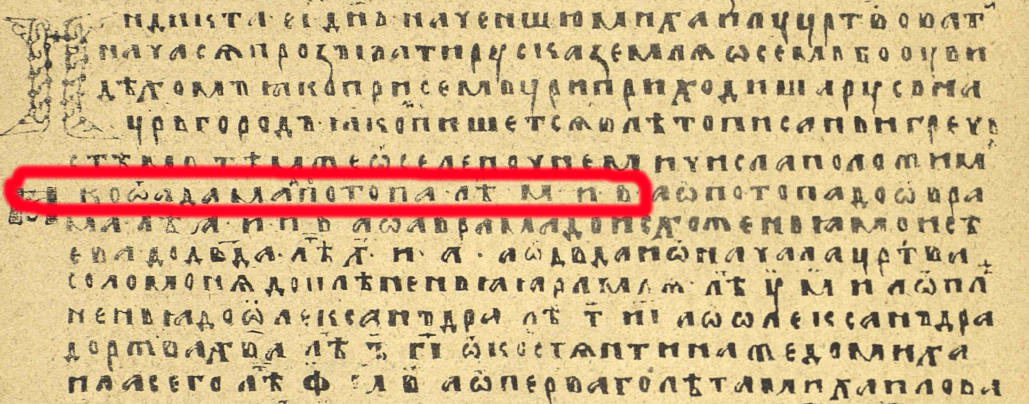
\includegraphics[width=\linewidth]{chast-colebanie-osnov/letois/lavr-sveto-01.jpg}
\end{center}

В светописное издание Лаврентьевской летописи, страницу 12. Промежуток лет от Адама до потопа задан так: «яко от адама до потопа лет 40 и 2», цифры обозначены буквами М и В.

Это 42.

А в обработанном издании? Там указано число 2242.

Разница между подлинником и обработанным текстом – 2200 лет.

Что это значит? Много чего! Выходит, в Лаврентьевском списке, даты вовсе не по счету Византийской эры. Временная шкала, используемая в Лаврентьевском списке, сдвигается на 2200 лет – при проверке первого же «слагаемого» из Росписного слоя в подлиннике! А значит, Иисус рождается на 2200 лет от сотворения мира раньше – по эре, используемой в Лаврентьевской летописи.

Я не изучал еще на этот счет светописные издания других летописей, кроме Лаврентьевской, но полагаю, что в подлинниках откроется много любопытного касаемо используемых эр и датировок.

Что же ученые? Проводят ли они нехитрые вычисления, доступные любому школьнику, чтобы определить, какое летосчисление применено в каждой отдельной летописи?

Нет. Они просто берут данные из Годового слоя, да еще обработанного правщиками изданий ПСРЛ, и по заученной формуле переводят числа из одной эры в другую. С данными из подлинников, а также с данными из Росписного слоя никто не работает.

Существует довольно мало книг о хронологии русских летописей, в эти мутные воды редко кто решается войти. Да и, мало кому приходит в голову выяснять, как же летописец считал годы, каким способом.

Одна из основных работ на эту тему, «Хронология русского летописания» Николая Георгиевича Бережкова, вышла в 1963 году смешным по тем временам тиражом – 1600 экземпляров. Это указывает еще и на степень востребованности историками подобных трудов. Бережков занимался вопросом, положенным им в название книги, с 1939 года.

Выявлены ли в «Хронологии русского летописания» слои летосчисления? Нет. Соответственно, не проведена проверка данных из этих слоев на соответствие друг другу. Какие числовые данные использованы в книге? Из обработанных изданий летописей. А мы знаем, что в подлинниках числа оказываются другими.

И здание науки стоит на зыбучем песке.

На всех страницах Бережков предполагает, что счет лет во всех рассматриваемых им летописях отличается только по годовому стилю – сентябрьскому, мартовскому и ультрамартовскому. И все вычисления крутятся около числа 5508.

Веками длится правка чисел в летописях. Веками же ученые используют эти правленные-переправленные числа, даже не помышляя о проверке, о том, чтобы определить, как даты появлялись в летописях.

Первое привело к тому, что у нас нет никаких четких датировок давних летописных событий. Второе – что мы используем ошибочные датировки всех событий вообще, включая современные, потому что числовое значение года рождения Христа, определенное в рамках «нашей эры» – тоже вычислено на основании чисел, взятых в мешанине различных летосчислений.

Казалось бы, современная наука отошла от религии, и ученые изучают следы явлений, произошедших, как полагают, за миллионы лет до нашей эры. Находят, допустим, скелеты динозавров, и говорят – динозавры жили 200 миллионов лет назад. Или 100 миллионов. И те же ученые, не моргнув глазом, используют временную шкалу, основанную на сведениях Библии о сотворении мира в предшествующие нам 10 тысяч лет. Так что это, вера или наука? Или наука и есть вера?

В моей ненаучной книге я вынужден делать много оговорок об использовании данных из разных источников. Как использую, почему, и указывать степень своего доверия к приводимым сведениям. Увы, я не имел сил и рвения затеять сверку всех чисел из доступных мне светописных копий – сверку как между копиями, так и с «подготовленными» учеными текстам в изданиях ПСРЛ. Делал это отрывочно и по мере надобности, а должно быть у общей картины выявил бы любопытные закономерности, или вообще запутался.

В целом для цитат, если не разбираю нечто крайне важное, я обращаюсь к «подготовленному» изданию 1908 года Ипатьевского списка, да изданию 1926-1928 Лавреньевского, это из имеющихся у меня изданий лучшие, кроме светописных.

А что мне делать с датами? Датам из каких списков отдавать предпочтение? Из какого слоя какой летописи? Нет у меня ответа, и вынужден я пользоваться датами общепринятыми, порицая оные и указывая на их шаткость.

Некоторые летописи содержат дополнительные сказания, такие как «Сказание о Словене и Русе и городе Словенске», где читаем:

\begin{quotation}
И в лето от сотворения света 3099 Словен и Рус с роды своими отлучишася от Ексинопонта, и идоша от роду своего и от братия своея.
\end{quotation}

Потирая руки, применяем известную формулу в общем ее виде. От летописного года отнимаем год 5508:\\

3099-5508=-2409\\

Это же 2409 год до нашей эры! Здесь одни ученые говорят – не может быть, выдумка новгородских книжников. А другие находят подтверждение следов древнейшей истории Славян.

Но разве мы знаем, какое летосчисление использовалось в «Сказании»? Давайте-ка на пробу применим к нему летосчисление не Византийской эры, а другое. Например, из римских хронографов. У них сотворение мира отнесено к 3948 году до нашей эры. Давайте подсчитаем. От летописного года 3099 отнимем 3948. Получим 849 год до нашей эры. Тоже звучит фантастически, но всё же в меньшей степени, чем третье тысячелетие до нашей эры.

Может быть, в истинном летосчислении «Сказания», число 3099 при переводе на «от рождества Христова», относилось бы, скажем, к девятому веку нашей эры.

Время и место. Так называется замечательный роман Юрия Трифонова, однако от времени и места зависит счет лет. Из-за того, что в летописи попали сведения из разрозненных источников, зачастую трудно сказать, насколько верна эта дата по отношению к Годовому слою летописи-приемника. И чем глубже в историю, тем более летописные даты теряют основательность.

А какое было летосчисление до принятия Владимиром христианства\footnote{Читатель, да услышь ехидство в сем вопросе!}? Повесть временных лет охватывает часть времен поганских. Нестор не был им свидетелем и пользовался чужими рассказами. Надо полагать, в этих его источниках существовали свои летосчисления. Какие? Загадка.

Но хорошо.

Мы сейчас ведет счет лет «от нашей эры», то бишь от рождества Христова. Привычно и понятно.

Но ведь разные народы в разное время перешли на такое летосчисление. Однако положим, кто-то раньше других. Сейчас мы, после цепочки произведенных во глубине веков вычислений, пользуемся годом рождения Христа, вычисленным монахом Дионисием Малым\footnote{Скиф Дионисий слыл образованнейшим духовным лицом Рима во времена папы Иоанна I. В математических расчетах Дионисий использовал ноль, чего среди его современников не водилось.}. Дионисий при вычислениях считал годы по современной ему Диоклетианской эре. Ею пользовались христиане Египетской Александрийской церкви, а ныне Коптская православная церковь. Вопрос, насколько верно вычисление Дионисия, оставим в стороне. Эру же «от рождества Христова» впервые ввел в обиход – в своих научных трудах – другой монах, Бэда (Beda Venerabilis).

Когда в какой-то стране возникала надобность перейти на эру «от рождества Христова», то соотносили рождество Христово в счете лет Диоклетианской эры с годом рождества Христова по местному летосчислению. Но мы уже видели на примере русских летописей, что год рождения Христа в них, в зависимости от списка, легко прыгает на тысячу лет. События могут смещаться – в письменной истории – на тысячу лет относительно рождества Христова, нашей эры. 

Поскольку приняли полагать, что числа в одних летописях верны, а в других ошибочны, то в основе датировки событий лежит вера. Вера в определенную летопись.

А когда начали вести счет годам от рождения Христа? С дня его рождения? Нет. Сразу после его смерти? Тоже нет. Когда же?

Столетия спустя.

Как вообще можно узнать, когда родился Иисус?  Выясним, какие временные привязки существуют у этого события.

В Библии не написано, что в таком-то году от сотворения мира. Но вроде бы есть много способов  вычислить год рождения\footnote{Способ с привлечением царя Ирода не прокатит – наместников Иудеи под таким именем было 9 – целая династия, и все Ироды.}. Например, известно, что судили Иисуса при Понтии Пилате (Pontius Pilatus), пятом по счету римском управителе провинции Иудеи. Историческое лицо. Когда он родился? 

Единственные, по большому счету, известные упоминания о нем в давних источниках, помимо Нового Завета, находим у римских историков Тацита и Флавия Иосифа. Тацит просто сообщает в своих «Анналах», что Христа казнил «при Тиберии прокуратор Понтий Пилат». Флавий Иосиф перечисляет римских наместников Иудеи, среди них Пилата. Понятное дело, что оба историка в лучших традициях своего времени не используют даты, но делают отсылки к правлению императоров.

А даты их правления, худо-бедно, с некоторых пор появляются в истории, причем поначалу в летосчислении «местных» эр.

На каком-то этапе развития человечества, возникла необходимость эти местные летосчисления соотнести между собой. И каждый ученый, светский или церковный, делал по-своему. А многие не делали, ибо трудно до невозможности. Ведь надо увязать не просто летосчисления, но и календари.

До революции 1917 года, у нас использовался юлианский календарь – его счет дней года известен как «старый стиль», а год начинался с марта (потом начало года перенесли на сентябрь). Имя своё календарь получил от Юлия Цезаря, при коем был введен в обиход.

Сейчас мы используем григорианский календарь. Разница между днями обоих календарей медленно растет – поначалу это было 10 дней, в 1900-2100 годах составляет 13 дней, потом увеличится до 14, а с 2200 года до 15. Поэтому наш странный праздник «старый Новый год» приходится на григорианское 13 января, что по юлианскому календарю – 31 декабря. Ибо от 13 января отнимаем разницу счета дней в этих календарях, равную 13.

Французский ученый Жозеф Скалигер (Joseph Justus Scali\-ger, 1540-1609) ввёл в обиход искусственную эру – ее называют теперь эрой Скалигера или юлианским периодом. За начало этой эры, в рамках юлианского календаря (системы счета дней), Скалигер положил (в пересчете на современную нам эру) 4713 год до нашей эры. Число взято не с потолка, а является произведением множителей 28*18*15, имеющих важные календарные и астрономические значения.

Скалигер в своих работах «Сочинении об исправлении хронологии» и «Сокровищнице хронологии» предложил таблицы перевода дат из различных эр в «свою», таким образом ученые получили в руки средство преобразования дат в привычные, переводя сначала дату в эру Скалигера, а затем из эры Скалигера – в нашу, основание которой тоже вычислено цепочкой таблиц и формул. 

Любое звено этой цепочки может быть ошибочно.

В эре Скалигера все дни (в смысле дня, определяемом юлианским календарем) последовательно нумеруются. Ученые берут какую-нибудь другую эру, например Набонассара, и вычисляют, на какой по счету день эры Скалигера приходится первый день эры Набонассара. Теперь даты, выраженные в счете лет Набонассара, можно соотносить с эрой Скалигера, а через нее – с нашей эрой.

Таким образом, подобные вычисления основаны на пользовании таблицами Скалигера. Быть может, он предлагает алгоритм, способ, по которому сам получил значения в таблицах? Допустим, зная правила умножения, мы можем составить таблицу умножения. А какие правила использовал Скалигер для своих таблиц? Он не пишет. А ведь хорошо бы знать, чтобы проверить!

Последователем Скалигера, в 17 веке, был тоже француз, иезуитский теолог Дионисий Петавиус. В своих трудах по хронологии он выстроил картину истории мира, расположив события по годам, используя как опорные события библейское сотворение мира и рождество Христово. Например, согласно Петавиусу, всемирный потоп случился на 1656 году от сотворения мира, и в 2329 году до рождества Христова.

Сравним с данными «удобочитаемого» издания Ипатьевской летописи. Потоп – 2242 год от сотворения мира, и 3212 лет до рождества Христова.

Петавиус давал также годы по эре Скалигера. Основные сочинения Петавиуса в области хронологии –  «Opus de doctrina temporum» и «Rationarium Temporum» – непревзойденные по охвату событий труды, где расписывается история человечества от сотворения мира и до времени самого Петавиуса. Упорядочение всего по годам! Какая адова работа проделана!

В веках, которые мы знаем как 15-17, ученые Европы принялись разбираться в летосчислениях разных народов, пытались сопоставлять. Год рождения Христа вроде бы уже имели, однако с привязкой – от основания Рима, что порождало несколько вариантов.

Скалигер, как показалось, внес некоторую ясность и предложил способ соотносить эры, упорядочивая историю. По Скалигеру, мир был сотворен за 3949 лет до рождения Христа.

Петавиус, продолживший дело Скалигера, применил его таблицы, разложив по ним события мировой истории. Петавиус внес также исправления. Он полагал, будто Иисус родился за 3984 года после сотворения мира. Начало эры Скалигера (Юлианского периода) имеет привязку – 764-й год до сотворения мира. Сдвиг Петавиусом времени сотворения мира означал «исправление» начала Юлианского периода – Петавиус соотнес его с 729 годом до сотворения мира.

Наконец, Джеймс Ашер в 17 веке поместил сотворение мира на расстояние 4003 лет до рождения Христа, и начало Юлианского периода связал с 710 годом до сотворения мира. Подобных чисел держался и другой ученый того времени, Джон Лайтфут.

Вооруженные таблицами и работами друг друга, христианские ученые-хронологи честно трудились над упорядочением истории, то бишь расставляя по годам события, описанные в разных источниках. Расставляя по годам «от сотворения мира» и от «рождества Христова», невзирая на то, что представления об этом у разных ученых были разные.

Но постепенно все стали приходить к некоему согласию. А оторванные, лежащие где-то в прошлом военные походы Александра Македонского, большой пожар в Риме при императоре Нероне, интриги византийского двора при Цимисхии, и даже вечно враждующие ярлы и бонды из скандинавских саг обрели четкую прописку в истории, получив свои года.

Сейчас у нас некоторый год, скажем, 2015 или 2200.  Я не знаю, когда вы читаете эти строки. Находясь, допустим, в 2066 году мы можем двигаться по одному году назад, и читая документы за эти годы, выяснять историю определенной страны. Время, для которого и ниже которого документы заканчиваются – хронологическая муть. Датировки событий, относящиеся к ней, вычислены. А мы видим, какая невероятная путаница лежит в основе этих вычислений.

Посему год 2022, или год 2200 – не более чем удобная условность для счета лет. 2022 на деле может не означать, что Христос родился 2022 лет назад. Мы не «досчитаем» назад до рождения Христа, у нас нет непрерывной цепочки датированных документов, тянущейся к этому событию. Таким же образом год допустим 860-й, приуроченный к чему-то в учебнике, может не означать, что такое-то событие случилось в 860 году нашей эры.

Далее в этой книге, конечно же, будут встречаться даты. Я согласен с относительной верностью дат, события которых записаны в то же время. Например, знаменитый краевед Киева Николай Закревский родился в 1805 году. И в какой-нибудь церковной книге был записан день его рождения. Тот год современники считали 1805-м.

Летописные годы из Повести временных лет, вплоть до Владимира, Ярослава и пожалуй несколько далее – как к ним относиться? Там же разнобой в списках! Что мне, все варианты перечислять? И каждый переводить в «нашу эру»? А на основании какого слоя – Царей, Росписного или Годового? А может Индиктов?

Ученым проще – они взяли книжку коллеги или предшественника, там готовые числа, и никаких вариантов. Верь им, бери да используй! А я не знаю, какие числа правильные. Я как мог дошел вниз, к доступному мне основанию, и не знаю, каким числам доверять, каким нет.

Поэтому я решил так. Даты буду приводить как в Годовом слое источников, принимая за таковые обработанные тексты из Полного Собрания Русских Летописей. Да и что толку даже от подлинников, если в них разные летосчисления и даты? Разные!

На вопрос, какое же летосчисление верное, и как по годам «нашей эры» разложить летописи разных народов, предания, саги, я отвечу просто – никак. Отсутствие четкой основы современного летосчисления. Слабая взаимосвязь давних источников. Разнобой летосчислений и числовых значений в пределах даже источников одного вида (например русских летописей).

Можно перебросить мостки между некоторыми летописями и сагами. У нас Ярослав, у них – Ярицлейв. Но это уровень слоя Царей. Правы были Греки, что не заморачивались и применяли в своих сочинениях этот слой!

Благодаря путанице дат, если не доверять научной хронологии, то вполне можно предположить – однако ни проверить, ни опровергнуть – что, допустим, поход аргонавтов за Золотым Руном происходил во времена князя Кия. Ведь нельзя же четко сказать, когда ходили за Золотым Руном, хотя историки относят сие событие, подробно описанное Греками, к сказкам.

Кстати о сказках. Прошлое многих народов уходит корнями в то, что ученые именуют мифом, легендой.

Про былое Киева сложно говорить, оно до Кия словно отрезано. А вот возьмем историю Ирландии. Ее исторические предания наука делит на сказочные и настоящие. Хотя в самих преданиях такого разделения нет. Существует список правителей Ирландии – и тоже, одних правителей ученые называют настоящими, других – легендарными! А почему?

В старейших известных временах Ирландии, люди – лишь одни из действующих лиц. В подробно описанной череде событий действуют представители множества народов, среди них основные – Фир Болг (Фирболг), Фомойры, Туаха Дэ Дананн (Tuatha De Danann, что обычно, полагаю ошибочно, переводят как «Народы богини Дану») и клан Мила, да вот только... К простым людям относятся определенно лишь представители клана Мила.

Прежде враждовавшие, Туаха Дэ Дананн и Фомойры потом смешались. Позже Ирландию завоевывали люди, а именно «сыновья Мила» или «клан Мила» – Скифы-выходцы из Египта, прибывшие через Испанию. Затем Туаха Дэ Дананн совершили странный исход с лица земли. Его смысл ускользает из преданий, но сходен с исходом сказочного народа «чуди белоглазой». После своего сокрытия, представители Туаха Дэ Дананн постепенно прослыли эльфами или фэйри, чудесным народом.

%проявляют те же свойства, что эльфы, однако я не уверен, что полное отождествление будет точным, хотя среди исследователей этого вопроса прижилось считать народы богини Дану эльфами.

Я понимаю, сразу перед глазами встает остроухий образ из фантастических произведений, однако нет никаких указаний на необычность внешности Туаха Дэ Дананн, в отличие от Фомойров. Туаха Дэ Дананн, однако, обладали некими способностями, которые люди именовали волшебными.

Так вот, известно 142 правителя Ирландии, которых ученые относят к выдуманным. Известны годы их правления, составлены генеалогические деревья, кто чей сын, дочь или брат, но вот беда, такой-то правитель – из Туаха Дэ Дананн или Фомойров.

Для примера, и сравнения с нашими летописями, приведу выдержку из одной ирландской летописи – Анналов королевства Ирландии (Annála Ríoghachta Éireann). Их составили в 17 веке, пользуясь разными источниками, ученые монахи ордена францисканцев. Их кстати не беспокоило, что речь в значительной части Анналов идет про «волшебные» народы.

Вот мой перевод самого начала этой ирландской летописи, выполненный с английского перевода 1856 года (семитомник Annals of The Kingdom Of Ireland by the four masters)\cite{annals4mast}. Повествуется о начале заселения Ирландии. Имена оставляю в английском написании:

\begin{quotation}
От сотворения мира до года Потопа, 2242 лет. Сорок дней до Потопа, Ceasair\footnote{В анналах Clonmacnoise, Ceasair или Caesarea названа племянницей Ноя, предупрежденной о Потопе.} прибыла в Ирландию с пятьюдесятью девушками и тремя мужчинами; Bith, Ladhra, и Fintain – их имена. Ladhra умер в Ard-Ladhrann, и от него такое название. Он был первым, кто умер в Ирландии. Bith умер в Sliabh Beatha, и был погребен в карне\footnote{Carn – курган из камней.} Sliabh Beatha\footnote{Примечание 1593 года нашей эры: этот курган существует поныне и расположен на той части горы Sliabh Beatha, что тянется через часть церковного прихода Clones, относящегося к графству Fermanagh.}, и по нему так названа гора. 

Ceasair умерла в Cuil-Ceasra, в Connaught, и была погребена в Carn-Caesra. А по Fintain прозван Feart-Fintain, над Loch Deirgdheirc.

От Потопа до времени, когда Parthalon завладел Ирландией, 278 лет; а от сотворения мира, 2520.

В году 2520 от сотворения мира Parthalon прибыл в Ирландию\footnote{В анналах Clonmacnoise соотносят прибытие Parthalon с 21-м годом жизни Авраама, и с 12-м годом правления ассирийской императрицы Семирамиды, однако переносят время к 313 году после Потопа.}. С ним были трое его сыновей, вожди: Slainge, Laighlinne, и Rudhraidhe; а также четверо их жен: Dealgnat, Nerbha, Cioch\-bha, и Cerbnad\footnote{По латинскому сочинению Historia Brittonum, Partholomus приплыл из Испании, а с ним было 1000 человек.}.

Год 2527 от сотворения мира. Fea, сын Torton, сын Sru, умер в этом году в Magh-Fea и был погребен в Dolrai-Daighe-Fea; по его имени и названа эта равнина.

Году 2530 от сотворения мира. В этом году произошла первая битва в Ирландии; Cical Grigenchosach, сын Goll, сын Garbh, из народа Фомойров, и его мать, прибыли в Ирландию с восемью сотнями воинов, и было сражение между ними и войском Parthalon в Sleamhnai-Maighe-Ithe, где все Фомойры были побеждены.
\end{quotation}

Далее ирландская летопись продолжает скрупулезно повествовать, кто когда прибыл, с кем воевал, когда умер, и так далее. Пропустим череду лет:

\begin{quotation}
От сотворения мира, 3303. Десятый год правления Eochaidh, сына Erc; и это был последний год его правления, ибо Туаха Дэ Дананн прибыли, чтобы отбить Ирландию у Фирболг\footnote{Оба народа некоторые источники относят к потомкам Афета, сына Ноя.}; и они воевали друг с другом в Magh-Tuireadh, Conmainche-Cuile-Toladh, Connaught. И король Eochaidh, сын Erc, был убит тремя сыновьями Neimhidh, сына Badhrai, из Туаха Дэ Дананн. Этих трех сыновей звали: Ceasarb, Luamh и Luachra.

Фир Болг были уничтожены в этой битве. Как сказано ранее, Eochaidh стал последним королем от Фир Болг в Ирландии. Всего их правило предположительно девять, и 37 лет длилось их правление над Ирландией.

Год от сотворения мира 3304. Первый год правления в Ирландии Breas. Туаха Дэ Дананн передали власть ему после победы в битве Magh-Tuireadh Conga, пока рука Nuandhat не будет излечена. 

Год от сотворения мира 3310. Это был седьмой год правления Breas в Ирландии, когда он передал власть Nuadhat, после того, как Diancecht при помощи Creidne приделал ему серебряную руку\footnote{Диоген Лаэртский сообщал про Пифагора: «Рассказывают, что однажды, когда он разделся, у него увидели золотое бедро».}.\end{quotation}

На этом, пожалуй, остановлюсь. Дальше идет в том же духе. Это вполне летописные сведения, ничуть не лучше и не хуже наших отечественных. У нас в летописях чудеса похлеще серебряной руки бывают.

Подобно сагам и русских летописям, в анналах Ирландии есть примечания, как называется то или иное место нынче (при составителе хроники), где оно расположено. Заметно сходство давних источников, стремление их составителей перебросить мостки между прошлым и настоящим.
 
Что не нравится ученым в ранних ирландских анналах?

Первым делом Всемирный Потоп. Ведь сначала в Ирландию, до Потопа, приплывает Ceasair. После Потопа – Parthalon. Оба вроде бы люди. Иное не указано. Затем Parthalon воюет с Cical Grigenchosach, сыном Goll (а тот – сын Garbh).

Cical Grigenchosach не человек в привычном нам значении слова, а относится к Фомойрам. Языковеды Ирландии предполагают, что это название означает нечто вроде «живущие под морем», ибо «fo» это «под», а «muire» значит «море». Эти существа описываются по-разному – то красивые люди, то одноглазые и одноногие\footnote{Согласно представлениям давних Греков, циклопы и одноногие люди обитали в Скифии. Одноглазыми считались и песиголовцы.}, то люди с козлиными головами. Великаны и обычного размера.

Далее я выпустил из хроники много, и продолжил выдержку прибытием Туаха Дэ Дананн – в то время Ирландия находилась под властью народа Фир Болг. Фир Болг и Туаха Дэ Дананн выводятся в преданиях из общего рода, от Немеда\footnote{Нимед, Нымет, Немед, Нимез или Нимет. Согласно преданиям, был родом из Скифии.}, а в предка Немеду ставят Ноя. Замечу, что христианские хронографы поступали подобным образом даже с языческими божествами – так, в греческих хронографах Зевс, его отец Крон, да и все боги-олимпийцы вписаны в родословное дерево библейских героев, и Зевс не бог, а лишь правитель.

«Библейская» привязка может быть вызвана несколькими причинами. Первая, логическая – по Библии, после Потопа спасся только Ной и его сыновья, Афет, Хам и Сим. Стало быть все, кто появляются в истории после Потопа – их потомки. Другая – только увязкой с Библией эти сведения удалось сохранить в составе Анналов. Третья причина – речь идет об указании на местность, откуда происходят определенные народы, ибо по Библии, части света были поделены между Хамом, Симом и Афетом.
% – возможно, отголосок территориально-административного передела, произошедшего после Потопа. Что по сути и должно быть случиться, рано или поздно.
 
Туаха Дэ Дананн сражаются с Фир Болг, побеждают, правление временно передают Breas, пока Nuandhat не вылечит руку (сначала ему приделали серебряную, а потом отрастили настоящую живую). При этом, у Breas мать – из народа Фомойров.

Туаха Дэ Дананн и Фомойры скрылись загадочным образом – в местах, что для человеческого глаза выглядят холмами или развалинами, но для истинных обитателей городами и замками, либо же в холмах открываются входы в тайные чертоги. Эти народы продолжили, но редко, взаимодействовать с людьми и стали восприниматься как волшебный народ (фэйри), эльфы (элвы, альвы). Это не значит, что эльфами считали только совершивших переход Туаха Дэ Дананн и Фомойров.

У ирландцев, шотландцев, гаэльцев, уэльсцев слово «эльф» не было в ходу, пользовались именованиями вроде Мирный народ (Daoine Shi, Shi), Добрые соседи, Хорошие люди (Daoine matha), фэйри. Среди населения островов Оркни ходило слово «троу» (traw). 

Также среди шотландского народа островов Оркни считалось, что прежде там жили малорослые Пикти (Picti), от кото\-рых-то люди и научились варить эль. Однако современные ученые утверждают, будто Пикти были некими кельтами, обычного роста. Между тем написанное на латыни в 11 веке нашей эры сочинение Historia Norvegia говорит, что Пикты были ростом чуть более пигмеев и творили чудеса в построении укрепленных городов.

Название Picti происходит от их обычая покрывать тела татуировками. Пиктов уничтожили потомки клана Мила, Ск\'оты (разделившиеся сейчас на ирландцев и шотландцев), но прежнее название их страны, Pictland, первоначально держалось за нынешней Шотландией. Скоты, согласно средневековой Chronica De Origine Anti\-quorum Pictorum, полагали, что Пикты тоже родом из Скифии, как и сами Скоты.

На островах Оркни и вообще в Шотландии известны сложенные из камней жилища, называемые брохи (brochs). Они имели вид перевернутых горшков, от 5 до 13 метров высотой, с низким входом у основания и зачастую имели подземный этаж, для выполнения неких ритуалов. Между двойными стенами шла винтовая лестница, соединявшая этажи. Брох венчала коническая деревянная крыша. Всего в Шотландии найдено около 500 брохов, причем без следов насильственного разрушения – их просто оставили. Почему-то, когда-то.

\begin{center}
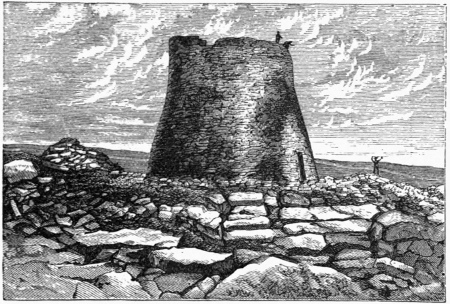
\includegraphics[width=\linewidth]{chast-colebanie-osnov/letois/fig160_197.jpg}
\textit{Broch of Mousa, Shetland.}
\end{center}

В статьях приводят замеры брохов – диаметр, высоту, но почему-то избегают сказать, какая была высота дверей. Но бывают и добросовестные ученые. Открываем книгу Джозефа Андерсона «Шотландия в поганские времена» («Scotland in pagan times», Joseph Anderson, 1881), по сути, сборник лекций. Лекция четвертая, «Устройство брохов». Рассматривается брох на острове Муса (Mousa), в Шетландии (архипелаг на северо-востоке Шотландии).

Про внешнюю дверь написано:

\begin{quotation}
Она на уровне земли, с юго-западной стороны, и около 5 футов 3 дюймов (1,524 метра) высотой и 2 фута 11 дюймов в ширину.
\end{quotation}

Далее идет описание, куда ведет тоннель от двери, то да сё, и потом описание внутренних помещений. Среди прочих там есть три комнатки, круглые, разной высоты – от 9 до 10 футов (2,7-3 метра), то есть можно не пригибаться, выше человека, но вот двери туда по три фута высотой и два в ширину, то есть 91 на 60 см. 

Существуют записки 17 века, шотландского священника городка Аберфойла, переводчика «Книги псалмов» на гаэльский, фольклориста Роберта Кирка (Robert Kirk), известные ныне под заголовком «The Secret Commonwe\-alth of Elves, Fauns and Fairies» («Тайное сообщество Элвов, Фаунов и Фэйри»).

Их предваряет описание:

\begin{quotation}
Природа и действия Подземного (и, в большей степени) Невидимого народа, известного под именем Элвов, Фаунов и Фэйри, или подобных, среди населения южной и восточной части Шотландии (Low-Country Scots), как они описаны теми, кто имеет Второе зрение; и теперь, для дальнейшего изучения, собранные и упорядоченные Осмотрительным исследователем среди Шотландско-Ирландского населения Шотландии. 
\end{quotation}

В этом небольшом произведении дается, с христианским оттенком, толкование необычных существ, способов их наблюдения, и взаимодействия с ними. Рассуждения, обобщения, многое размыто. Ощущаются недоговорки. По Кирку, фэйри или эльфы – отдельная раса, промежуточная между людьми и ангелами. У них тоже рождаются дети, бывают свои свадьбы и похороны. Среди них попадаются двойники людей из «нашего» мира.

Считается, что Кирк умер в 1692 году. И вот его преемник, священник Патрик Грэхем, в своем краеведческом путеводителе 1810 года «Sketches Descriptive of Picturesque Scenery, on the Southern Confines of Perthshi\-re», где немало места уделено фэйри, пишет, что Кирк вообще-то и не умер.

%Уолтер Скотт в своих «Письмах о демонологии и ведовстве» (Letters On Demonology And Witchcraft), изданных в первой половине 19 века пишет, со слов священника Патрика Грэхема из Абэрфойла

14 мая 1692 года, вечером, Роберт Кирк, отправился в одной ночной сорочке на так называемый Дан-ши, Doon Hill или холм Фэйри, небольшой пологий холм, что находился поблизости на запад от дома священника. Этот холм, поросший соснами и прочими деревьями, сейчас служит местной зловещей достопримечательностью.

На холме Роберт Кирк впал в состояние, которое сочли смертью, хотя, как замечает Вальтер Скотт в «Письмах о демонологии и ведовстве» (Letters On Demonology And Witchcraft), люди знающие могли бы определить в этом обморок, вызванный сверхъестественным влиянием народа, границы чьего владения он преступил. 

Роберта Кирка похоронили, однако после этого он неким образом явился, в той же ночной рубашке, одному из своих родственников и отправил того к Грэхему Дачрейскому (Duchray). Родич, с коему явился Кирк, тоже был родственником Грэхему Дачрейскому. Кирк поручил родичу следующее: «Иди к моему двоюродному брату Дачрэю и скажи ему, что я не мертв, я упал в обморок, и был перенесен в страну Фэйри, где теперь и нахожусь. Скажи ему, что когда он и мои друзья соберутся на крещении моего сына\footnote{Кирк оставил жену беременной.}, я появлюсь в помещении. Тогда, если Дачрэй бросит  над моей головой нож который он держит в руке, я буду освобожден и вернусь к обществу людей».

Родич однако не спешил передавать это сообщение. Тогда Кирк явился к нему повторно, угрожая преследовать его днем и ночью, если тот не передаст сообщение. Родственник наконец выполнил обещанное.

После церемонии крещения, все уселись за столом. Тут, якобы покойный, Роберт Кирк вошел в комнату через одну из дверей, но лорд Дачрэй по какой-то причине не бросил нож как было условлено. Роберт Кирк вышел через другую дверь и больше его не видели.

%, что смерть Кирка была необычной. Под вечер он вышел на прогулку по соседнему холму фэйри (dun-shi), и был найден в бессознательном состоянии, которое приняли за смерть. Преподобный Грэхем отметил, что знающие поняли бы, что это состояние вызвано сверхъестественным влиянием людей, чьи границы Кирк нарушил.

%После похорон, Кирк однако неким образом посетил родича, и попросил его передать на словах послание их общему двоюродному брату Грэхему из Дачрэя. Дескать, Кирк не мёртв, а пленен в стране Фэйри (Fairyland), и чтобы он смог вернуться, надо выполнить следующее. Жена Кирка осталась беременной. Когда она родит, Кирк будет при крещении младенца присутствовать в комнате. Тогда же брат должен бросить нож или кинжал поверх головы Кирка, и тот сможет вернуться к людям\footnote{Послание Кирка: «Say to Duchray, who is my cousin as well as your own, that I am not dead, but a captive in Fairyland, and only one chance remains for my liberation. When the posthumous child, of which my wife has been delivered since my disappearance, shall be brought to baptism, I will appear in the room, when, if Duchray shall throw over my head the knife or dirk which he holds in his hand, I may be restored to society; but if this opportunity is neglected, I am lost for ever.» – по Walter Scott, Letters On Demonology And Witchcraft.}.

%Кирк в самом деле появился на крещении, его видели, но Грэхем не выполнил просьбу, и Кирк лишился возможности вернуться.

Понятие «эльфов» и «фэйри» довольно размытое, отличается от местности к местности, и является общим названием, а не обозначением определенного вида существ. Можно сказать, что к эльфами относят сообщества перешедших в некий иной режим существования людей (и представителей других биологических видов) с особыми способностями, как Туаха де Дананн, а также просто некоторых умерших (подобное представление бытует у Славян в связи с русалками). Будучи в этом ином режиме существования, они изредка взаимодействуют с нами, обычно в особых местах и условиях.

%Например, Исландцы делили своих «альвов» на черных (подземных) и светлых (живут в Алфхэйме). Бытовало и мнение о трех видах, выраженное Йоуном Гвюдмундссоном Ученым (Jón lærði Guðmundsson, 1574-1658) в рукописи «Собрание сведений и фактов для лучшего понимания Эдды» (1641)\cite{korabl01}: 

%\begin{quotation}
%Люди полагают также, что эльфы – это народ, делящийся на три рода, или имеющий три основных места обитания. Одно – в море. Второе – внутри земли или под землей, которое люди называют «Эльфо-мир», а иногда – подземный мир, что многие наши истории поясняют. И люди видят, что этот род не имеет носового хряща между ноздрями. Живут же они половину обычного нашего срока (на земле). Третий род, который мы называем Сокрытым Народом или льювлингами также населяет холмы и скалы; и часто сочетались они с нашим родом. Этот эльфийский род живет дольше, отличается красотой и имеет правильную форму, как у нас.
%\end{quotation}

С эльфами связано иное течение времени. Это проявляется в следующих случаях. Ребенок, рожденный от эльфов (чистый эльф или полукровка) растет быстрее (среди людей), нежели дитя человеческое.

Живые люди, попадавшие в мир эльфов (осознаю всю условность этого определения), возвращались в мир людей спустя долгие годы, при этом для них прошло совсем немного времени. Значит, в мире эльфов время течет медленнее, чем в нашем. Однако возвращаясь оттуда, некоторые люди быстро старели, едва не на глазах. 

Любопытно, что мы знаем еще один мир с иным течением времени – мир снов, в котором время течет быстрее нашего. Таким образом выстраивается цепочка «миров», различных по скорости времени. Расположу по возрастающей: мир эльфов → мир людей → мир снов.

Какое всё это имеет отношение к Киеву? А я непроста рассказываю, позже всплывет.

Некоторые из героев ирландских анналов и сказаний, например Луг, были обожествлены, стали языческими богами. Выдающаяся личность сегодня, через век ее почитают за божество, а спустя еще пару столетий, когда переменяется вера – уже называют демоном. 

Ирландским анналам повезло, их не сократили под корень, оставили ирландцам прошлое. Наши же летописи, относящиеся к Киеву, словно отрублены на уровне князя Кия. И кто знает, повествование о каких событиях мы бы прочитали за предшествующие годы, и какие бы люди – или нелюди – действовали в них?

Но заглянуть за эту черту таки возможно, ведь кроме летописей, существуют и другие, внешние источники.

\chapter{Аланы}

С годами меняется облик планеты. Народы расселяются, обретают другие имена, обычаи, веру и даже языки, сохраняя нечто старое и предлагая соседним народам свои слова, обычаи и веры взамен приобретенных.

В Чечне, в зеленом подгорьи, у берега реки Сунжи есть село Алхан-кала. В глубокое прошлое проросли его корни. А в 19 веке Чеченцы переселись отсюда к юго-востоку, по другую сторону реки, и основали Алхан-Юрт, а на месте прежней Алхан-калы возникла станица терских казаков Ермоловская. Некоторое время атаманил в ней дед моей бабушки по отцовской линии, Леонтий Никитин. В начале 1920-х станица забунтила вместе с прочими окрестными. И по приказу Орджоникидзе ее жителей кого выселили, кого услали. Прошли годы. Ныне это снова Алхан-кала, и обитают в ней Чеченцы.

В четырех километрах от Алхан-калы найдено крупнейшее в том краю городище – остатки города, в котором жили, как полагают, Аланы – народ, ответвившийся от Сарматов. Укрепление длиной в километр, обнесенное рвами, один из коих глубиной 9 метров. Мощеная булыжниками мостовая. Кто ходил по ней? Чья речь слышалась? А в окрестных селениях?

Тот же вопрос уместно задать о Киевщине.

Как принято считать, Киев основан братьями Кием, Хоривом, Щеком да сестрой их Лыбедью. Одни ученые принимают это летописное предание, другие опровергают. Нет общего мнения.

Вот знаменитый историк Василий Ключевский. Его живо изложенные лекции в печатном виде зачитывались до дыр. Ключевский оценивал основание Киева скромно, приурочивая его к Кию с братьями, невесть почему назвав их звероловами и поселив в некие однодворные деревни: 

\begin{quotation}
Так Киев возник из трех однодворных деревень с общим укрепленным убежищем, которые поставлены были тремя звероловами...
\end{quotation}

Историки, согласные в определенной мере с преданием о братьях, обычно далее того не идут. Заложили братья крепость – град Киев, и ладно. А прежде что тут было? Ученые уходят от прямого ответа. Отделываются размытыми словами. Да, первобытные стоянки времен палеолита. Да, защитные валы черняховской культуры. Черепки горшков трипольской культуры... Но город, дескать, возник только при Кие.

Пытливый Максим Берлинский в своем «Кратком описании Киева»\cite{berl01} предположил наличие тут города до основания крепости Киева, ссылаясь на Клавдия Птолемея, перечислявшего города, лежащие по Борисфену, как Греки называли Днепр\footnote{Наука использует два основных способа чтения букв древнегреческих текстов, «итацизм» да «этацизм». По первому, слово Βορυσθένης надо читать как Ворисфенес, по второму – Борисфенес. Однако никто точно не знает, каково было произношение у древних Греков. Кроме того, в переводах прижилось отбрасывание окончания «ес», остается лишь корень Борисфен. Можно считать, что любое название либо имя из давних сочинений Греков переведено приблизительно. Оно могло произноситься иначе! Кстати, согласно поэме римского императора Адриана, имя коня Цезаря было Борисфен Аланский.}:

\begin{quotation}
Птолемей, между прочими городами упоминает об Амадоке, стоявшем при повороте Днепра, по левую его сторону, близ какого-то озера, или вероятнее реки, что по его ландкарте придется при впадении Десны в Днепр. И по ту же сторону Днепра, выше сего, упоминает о находившемся городе Азагориум, может быть, от тогдашних тамошних жителей назывался Загорье.
\end{quotation}

А один из самых передовых людей времен Петра I, многообразный деятель Василий Татищев, трактуя некий вариант карты к «Географии» Птолемея, название Азагориум примерял к Переславлю, а вот Амадок – относил к Киеву.

Попробуем разобраться с этим сами, по трудам давних греческих историков и географов, а также правителей Византии. Все их труды относятся ко времени, когда в наших краях жили Скифы (они же Скиты) и Сарматы. Выяснение подробностей приведет нас к другим источникам, мы возьмем на вооружение свидетельства давних Арабов, Латинов, Французов, а также наших летописцев и толмачей.

Задача – не раскрыть тайны прошлого до конца, но пробовать найти подступы к этому прошлому. Сравним то, что говорит современная наука, с тем, что утверждают люди, общавшиеся со Скифами и другими народами древности непосредственно.

Спросите любого на улице, кто такие Скифы? Вообще-то прохожего это вообще не колышет. Но упрощенное представление таково – древний воинственный народ. Кочевали по степям, хоронили своих в курганах, были мастерами делать украшения из золота, снимали с врагов скальпы.

А что скажет наука? Она завороженно твердит, что Скифы – «ираноязычные племена», обитавшие в землях от Дона до Дуная с 8 века до нашей эры по 9 век нашей эры.

Отметим, что теперь на большей части этого пространства живут сплошь Славяне – Чехи, Поляки, Русские, Украинцы – словом все нынешние страны со славянским населением прежде составляли Скифию.

Летописец Нестор в Повести временных лет, перечислив славянские народы, что обитают в землях от Дунаю до Днепра, пишет, что до сего дня Греки называют эти места «Великая Скуфь» (Большая Скифия). И повторно он говорит, о составе похода Вещего Олега, что Олег набрал войско из народов Варяг, Словен, Чуди, Кривичей, Мери, Полян, Северов, Древлян, Радимичей, Хорватов, Дулебов, Тиверцов – «си вси звахуться Великая Скуфь» – поясняет Нестор.

Так выходит, Скифы – общее греческое название Славян? А как же «ираноязычные племена»? В пользу ираноязычия Скифов говорят, казалось бы, имена рек – Дунай, Дон, Днепр, Днестр, многочисленные Донцы (Северский, Липовый, Саженный) – где ученые усматривают скифское слово «дан», что переводят как «вода» либо «река». А «Днепр», он же «Данапр» – мол, это «дана» и «апр», два скифских слова, означающих вместе вода глубокая.

А предложу-ка две славянские трактовки речных имен. Мы имеем весьма мокрый корень «дно». Отсюда, кстати, и «тонуть» – «донуть», идти ко дну. Разница между звуками «т» и «д» невелика. При склонении, «дон» легко превращается в «дне». Далее, вот корень иного, временного рода – «день», «дни». Быть может, название большой реки составлялось из производного от слова «дней» и указания количества дней пути по этой реке, то есть известной длины реки. Все эти «пр», «стр» – не искаженные ли числа?

Что мы знаем о языке, на котором говорили Скифы? Всеволод Миллер и Василий Абаев в своих работах, справедливо полагая современных Осетинов потомками Скифов (через Сарматов и Аланов, Асов), скифский язык пытались восстановить посредством осетинских наречий – иронского и дигорского. 

А как же Великая Скуфь? В ее пределах скифский язык улетучился, не оставив иного следа, кроме названий рек?

%Но что дошло до наших дней от языка Скифов? Их имена в сочинениях на греческом
%Будто бы – названия рек. Что еще? Ничего.

%Две крайности. По одной Скифы – греческое название Славян. По другой – ираноязычные кочевники.

%Названия рек хорошее подтверждение тому, что Скифы пользовались словами с иранской основой для обозначения рек, лежащих на огромном расстоянии друг от друга. Причем имена эти сохраняются поныне, значит, были местными! Не называем же мы Днепр как древние Греки – Борисфеном. В русском и украинском языках примесь, трактуемая «иранской», касается не только воды, это еще и некоторые цвета.

Общепринятое знание сбивает с толку. Это ведь ученые, а не сами Скифы, сказали нам про иранские корни в названиях рек. Может они вовсе не иранские, а утраченные славянские, либо следы какого-то третьего языка. Как вообще языки влияют друг на друга? А подобно музыкальным жанрам, при этом степень возможного влияния зависит от совместимости жанров.

Наука полагает, что Скифов вытеснили Сарматы, тоже ираноязычные. И разделяет Скифов, Сарматов, да Славян – причем то временами, то происхождением. 

Но я больше доверяю давним Грекам. Они, в отличие от современных ученых, общались со Скифами. Есть что рассказать. Поэтому обратимся за сведениями к Геродоту, Страбону, Льву Диакону, Клавдию Птолемею и Плинию Старшему.

Хотел расставить эти источники по времени, однако из-за путаницы с летосчислением я не могу доверять общепринятым датировкам сих трудов, и способен упорядочить оные лишь относительно. Например, Страбон упоминает Геродота – значит, «История» Геродота написана раньше, чем «География» Страбона. Географические сведения Греков существенно отличаются не только от нынешних, но и друг от друга, что впрочем может отражать изменения, происходящие с местностью с течением времени, а не ошибочность представлений.

К рукописным сочинениям Греков нередко прилагались карты, однако неясно, составлены ли они по карте самого сочинителя, либо на основании его текста. Подлинники, начертанные Клавдием Птолемеем и другими остаются неизвестными, да и вряд ли сохранились бы. Пожары, сырость, прочие влияния окружающей среды, наконец невольный враг древних знаний – мыши.

Старинные карты кажутся на первый взгляд нелепыми. Причина тому, кроме ошибок, смешение источников современных составителю карты и источников буквально допотопных, отражающих состояние Земли до Потопа, который, сопровождаемый другими бедствиями, вполне мог служить причиной исчезновения одних гор и морей, возникновения других, переменить течения рек, не говоря уже о том, что с лица земли стёрлись целые страны. Но водная сеть меняется быстро и без привлечения Потопа.

Таким образом наиболее древние карты давали одновременно представление о Земле до Потопа и после, а с течением времени уточняясь новыми данными, лишались допотопных следов. Поэтому чем ближе к нам, тем менее фантастичны карты.

В историко-географических трудах Греки по-своему обозначали страны, города, реки, моря и озера. Порой эти названия были искаженными производными от местных именований. Либо чисто греческими. А может, по-гречески их тогда называли и тамошние обитатели. И сейчас исследователи ломают себе головы, что же подразумевали греки?

Например, Рипейские (Рифейские) горы. С ними ученые соотносят Урал, Кавказ и Тянь-шань. Каравай, каравай, кого хочешь – выбирай. Но и некоторые Греки, тот же Страбон, вообще сомневались в существовании таких гор!

В «Географии» Птолемея, где употреблена сеть координат, устье Борисфена (Днепра) лежит западнее реки Хипаниса (в отечественных переводах часто пишут: «Гипанис»). С Хипанисом отождествляют Южный Буг, однако у Птолемея это разные реки, он различает Хипанис и «Буц» (Buces). Современные толкователи обычно пишут – Птолемей ошибается, устье Буга западнее устья Днепра.

Но если считать устьем Днепра западную часть современного Днепровского лимана (куда впадает и Днепр, и Южный Буг), то устье Днепра таки западнее, чем устье Буга. А Греки так и считали.

Археологи уже давно и обстоятельно раскапывают  древний город Ольвию\footnote{46°41'33.0"N 31°54'13.0"E}. Она лежит под Николаевом, на берегу Южного Буга, примерно в 5 километрах выше его устья в Днепровском лимане. Это именно Ольвия, о чем свидетельствуют найденные там многочисленные надписи на греческом. Вырезанные в камне, они подтверждают различные права вроде этого\cite{olbia01}:

\begin{quotation} 
В добрый час! Ольвиополиты дали Ксантиппу, сыну Аристофонта, эрхиейцу, сыну Филополида, дейрадиоту – афинянам, им самим и потомкам их проксению, право гражданства, освобождение от пошлин на все товары, какие бы ни ввезли или не вывезли они сами, или их дети, или братья, у которых отцовское имущество общее, или слуги, и дали право входа в гавань и выхода из гавани и в мирное, и в военное время, без конфискации и без заключения договора.
\end{quotation} 

Здесь мы видим слова без перевода (дейрадиот, проксений) – их точное значение остается неясным поныне, посему оставляют как есть. А вот «ольвиополиты» значит «жители Ольвии». Эти ольвиополиты часто упомянуты в надписях Ольвии, и можно сделать однозначный вывод о названии города.

%Плиний в 26-й главе «Естественной истории» говорит:
Плиний в «Естественной истории» говорит:

\begin{quotation}
На расстоянии 120 миль от Тира лежит река Борисфен, с одноименным озером и народом, а также городом на материке, на расстоянии 15 миль от моря. Старые названия этого города Олвиополис и Милетополис.
\end{quotation}

Тир это Днестр. Есть на нем город Тирасполь, что подтверждает отождествление Днестра с Тиром.

Итак, по Плинию, в 15 милях от устья Днепра  лежит город Борисфен, другие названия коего – Ольвия и Милетополь. Местных жителей именовали Борисфенитами. При пересчете в километры, 15 миль Плиния – это примерно расстояние от устья Днепровского лимана до Ольвии. Стало быть, сей лиман Греки принимали за часть Днепра.

Страбон, в 7-й книге «Географии» сообщает:

\begin{quotation}
Дельта Борисфена (Βορυσθένης) судоходна на 600 стадий, а близко другая река, Хипанис (Ὕπανις), и остров перед устьем Борисфена, с портом. Если плыть по Борисфену 200 стадий будет одноименный с рекой город: он называется также Олвиа, большой торг, основанный Милисиами.
\end{quotation}

%Εἶτα Βορυσθένης ποταμὸς πλωτὸς ἐφ᾽ ἑξακοσίους σταδίους καὶ πλησίον ἄλλος ποταμὸς Ὕπανις καὶ νῆσος πρὸ τοῦ στόματος τοῦ Βορυσθένους, ἔχουσα λιμένα. Πλεύσαντι δὲ τὸν Βορυσθένη σταδίους διακοσίους ὁμώνυμος τῶι ποταμῶι πόλις· ἡ δ᾽ αὐτὴ καὶ Ὀλβία καλεῖται, μέγα ἐμπόριον, κτίσμα Μιλησίων.

Как видим, и здесь Ольвия помещена на берегу именно Днепра. Даже указано расстояние к ней – 200 стадий. А устье Борисфена судоходно (вероятно для морских, не речных кораблей) на 600 стадий. Сколько всё это в пересчете?

По представлениям науки, 1 стадия это... Различают разные стадии. Греческая, мол, 178 метров, олимпийская 192,3 метра, аттическая – 177,6, птолемеева – 185 метров, и прочие. Беда! 

Возьмем округленное 180 метров. Сколько будет в километрах – 200 стадий? 200*180/1000 = 36 километров. Это расстояние от устья Днепровского лимана до Ольвии. Итак, Греки однозначно полагали, что устье Днепра – это устье нашего Днепровского лимана. А вот Ольвия лежала на берегу этого «продленного» Днепра. Где тогда находилось устье Южного Буга, я не знаю.

Вычислим теперь, на какое расстояние от моря судоходна дельта Днепра во время Страбона. 600 стадий умножим на 180 метров – равно 108000 метров. 108 километров. Принимая за устье Днепра устье нынешнего Днепровского лимана, и что русло проходило так же, как ныне, у нас получится, что суда от моря могли подниматься по дельте Днепра  немногим, километров на 20, выше Херсона.

%Геродот, живший раньше Страбона, утверждает, что Днепр известен на 40 дней пути. Но к этому мы еще вернемся.

Однако, Днепр был известен и выше – Геродот говорит, что на сорок дней пути! Геродот из наших греческих источников древнейший. Считается, что он жил в пятом веке до нашей эры, но я полагаю, что не столь давно. В своей «Истории», в книге «Мельпомена» он рассказывает о походе царя Персов Дария на Скифов, и дает обстоятельное описание последних\cite{herodotus01}:

\begin{quotation}
По словам самих Скифов, они – юнейший из всех народов, и о своем происхождении рассказывают так: первым человеком в этой стране, тогда еще пустынной, был Таргитай\footnote{Такое же имя, искаженное в «Таргитий», встречаем у Фиофилакта Симокатты в «Истории», где Таргитий – посол Аваров, пришедший к Ромеям-византийцам за ежегодной данью для кагана Аваров. Прочие имена Аваров по этому сочинению: Сирмий, Баян, Турум, Спарзевгун, Кунаксолан, Тулдих. Впрочем, Симокатта считает европейских Аваров самозванцами, на деле представителями народов Уар и Хунны.}; родителями Таргитая они называют, чему я не верю, Зевса и дочь реки Борисфенеса. Такое происхождение приписывается Таргитаю.

У него было три сына: Липоксаис, Арпоксаис и самый младший Колаксаис. При жизни их упали с неба на скифскую землю золотые предметы: плуг, ярмо, секира и чаша.

Первым увидел эти предметы самый старший из братьев; он приблизился к ним с целью взять, но при его приближении золото воспламенилось, и он отступил назад. Затем подошел средний брат, но с золотом повторилось то же самое. Таким образом золото горением не своим не допустило к себе двух братьев; с приближением третьего, наимладшего брата золото потухло, и он отнес его к себе в дом. Поэтому старшие братья согласились уступить наимладшему все царство.

От Липоксаиса, рассказывают дальше, произошли те из Скифов, которые носят название рода Авхатов (Αὐχάται), от среднего, Арпоксаиса, произошли Скифы, именуемые Катиарами или Трапиями (Κατίαροί τε καὶ Τράσπιες), а от наимладшего, царя, те, что называются Паралатами (Παραλάται). 

Общее название всех Скифов, по имени царя их, Сколоты (Σκολότους); Скифами назвали их Эллины\footnote{Я бы перевел иначе: общее название этих варваров – Сколоты, то есть из царского рода (царствующие), а Скифами их назвали Эллины. σύμπασι δὲ εἶναι οὔνομα Σκολότους, τοῦ βασιλέος ἐπωνυμίην. Σκύθας δὲ Ἕλληνες ὠνόμασαν.}.

Так рассказывают Скифы о своем происхождении, полагая, что от начала их существования или от первого царя Таргитая до похода Дария прошло круглым счетом никак не больше тысячи лет.

Упомянутое выше священное золото цари оберегают  весьма ревниво и ежегодно благоговейно чтут его обильными жертвоприношениями.
\end{quotation}

Здесь Геродот называет Царскими (по-скифски Сколотами), не всех Скифов вообще, а три скифских народа, ветви Скифов: Катиары, Трапии и Паралаты. Были и другие народы Скифов, над которыми, надо полагать, при Дарии властвовали эти Царские Скифы.

Вероятно, именование Царских Скифов перемещалось позже со Сколотов на другой народ из числа Скифов. Был один правящий народ, собиравший дань, и его подчиненные. Приск Панийский из Фракии, состоявший в посольстве Максимина к Аттиле, в «Истории Готфов»\footnote{Приск попутно дает имена Царских скифов, помимо Аттилы: Васих, Курсих, Верих. Жену Аттилы зовут Крека. Если в мужских именах поменять «х» на «ч», получим ближе к славянским: Васич, Курсич, Верич.} относит к Скифам народы Унны (Хунны) и Готфы (Готы), однако различает эти два народа, а Уннов величает Царскими Скифами. Как я понимаю из описания Приском сборного скифского войска, Унны и Готфы были родственны, но Готфы находились в подчинении у более хищных Уннов. Не исключаю, что те, кто при Геродоте именовались Сколотами, во время Аттилы слыли Хуннами.

Скифские народы, по Геродоту, живут от Истра (Дуная) до Танаиса (Дона)\footnote{С Танаисом связана странность. Историк Иордан в «Гетике» говорит, что есть два Танаиса. Один, разделяющий Европу с Азией, начинается в Рифейских горах и впадает в Мэотийское болото (оно отождествляется с Азовским морем). Этот Танаис никогда не замерзает, в отличие от соседних рек, а также Мэотиды и Босфора. А другой Танаис рождается в Хриннских горах и впадает в Каспийское море.}. Он называет следующие реки Скифии, кажется по порядку соединения их устий с морем, с запада на восток: Истрон (Ἴστρον), Тирас (Τύρης), Хипанис (Ὕπανις), Борисфенес (Βορυσθένης), Пантикапес (Παντικάπης), Хипакирис (Ὑπάκυρις), Геррос (Γέρρος, рукав Борисфена, впадает в Ипакирис), Танаис (Τάναϊς)\footnote{Всё это греческие и «огреченные» названия, поэтому даю как в подлиннике. Однако видно, что например Дон, Дан превращен в Танаис заменой «д» на «т» и добавлением «аис». «Тирас» же – греческое именование Днестра, ничего не переиначено.}. Про Хипанис сказано ранее, а отождествление Пантикапеса, Хипакириса и Герроса с современными названиями остается загадкой поныне.

Про Скифов Геродот пишет:

\begin{quotation}
Ведь у Скифов нет ни городов, ни укреплений, и свои жилища они возят с собой. Все они конные лучники и промышляют не земледелием, а скотоводством; их жилища – кибитки.
\end{quotation}

Казалось бы, здесь говорится вообще обо всех Скифах как о кочевниках. Однако почитаем «Историю» дальше. Я буду делать выдержки и свои отступления, чтобы обсудить. Среди скифских рек Геродот особенно хвалит Днепр:

\begin{quotation}
Четвертая река Борисфенес – из скифских рек после Истра наибольшая и, по нашему мнению, самая богатая полезными предметами не только между скифскими реками, но между всеми вообще, кроме впрочем египетского Нила; с этим последним не может идти в сравнение никакая другая река.

Но из прочих рек Борисфенес наиболее прибылен: он доставляет прекраснейшие и роскошнейшие пастбища для скота, превосходную рыбу в большом изобилии, вода его на вкус очень приятна, чиста, тогда как рядом с ним текущие реки имеют мутную воду;
\end{quotation}

Природные ресурсы уже тогда играли важнейшую роль в жизни человечества. Как сейчас воюют за нефть, так прежде ценностью были пастбища. Особенно для Скифов-скотоводов.

\begin{quotation}
Вдоль его тянутся превосходные пахотные поля или растет очень высокая трава в тех местах, где не засевается хлеб.
\end{quotation}

Кто же пашет эту землю, если Скифы, по словам Геродота – скотоводы? Поскольку здесь существуют посевы и Скифы, значит, среди них есть земледельцы. Верно:

\begin{quotation}
До местности Герров, куда сорок дней плавания, Борисфенес течет, как известно, с севера; страны, через которые он протекает выше этого пункта, никому неведомы; несомненно только, что до области Скифов земледельцев он протекает через пустыню, а Скифы эти живут вдоль его на десять дней плавания.
\end{quotation}

Прежде чем касаться 40 дней плавания, обсудим Скифов-земледельцев. Иногда в переводах звучит Скифы-пахари, или Скифы-георги. В подлиннике – γεωργοὶ Σκύθ\-αι. Георг, Георгий в переводе с греческого значит «земледелец» или «пахарь».

Византийский император Константин Багрянородный, живший позже Геродота, знал около порогов Днепра остров, именуя его «остров святого Георгия». Почти все исследователи сопоставляют его с Хортицей. Об этом позже. Вероятно, остров так назывался не от святого Георгия, но потому, что рядом жили Скифы-георги. 

Каких еще Скифов различали Греки? О Царских мы уже слышали. Иное их название – Василиды (от слова «василевс» – царь, правитель). Кочевых же скифов именовали Номадами. Впрочем, Геродот считал Царских Скифов кочевыми. Продолжим разбирать его слова дальше. Моё толкование несколько отягощено знаниями из других источников, в частности про пахарей, ибо я знаю, что они жили в низовьях Днепра, а из приведенного ранее сообщения Геродота этого нельзя вывести однозначно.

Итак, вверх по Днепру на 10 дней плавания лежат земли Скифов-земледельцев. Туда Днепр течет через «пустыню» – голую степь ли, пески ли, неясно. А вообще Днепр известен на 40 дней плавания, до местности Герр (Геррос, Γέρρος), куда Днепр течет с севера. Что выше Герров – никому не ведомо.

Кроме того,

\begin{quotation}
Седьмая река – Герр вытекает из Борисфена в том месте, до которого течение Борисфена известно. Ответвляется она в этом месте, а название ее, общее с местностью – Герр. Течет эта река к морю, образуя границу между землями кочевых и царских скифов, и потом впадает в Хипакирис.
\end{quotation}

Сейчас мы не знаем никакого рукава Днепра, который бы отделялся от него и впадал в другую реку (таинственный Хипакирис), соединенную с морем. Однако, насколько я понимаю, река Герр отделялась от Днепра на 40-м дне пути.

Сколько в километрах будет «40 дней плавания»? Это невозможно вычислить точно. Неясно, с какой скоростью передвигалось судно. Допустим, 5 километров в час. В дне 24 часа, но целый день не плыли. Положим, 12 часов плыли, 12 спали. Каждый день, таким образом, лодка проходит 12*5=60 километров. За 40 дней она пройдет, 40*60=2400 километров. Современная длина Днепра равна 2285 километрам.

Меняя при подсчете скорость, мы можем подогнать 40 дней пути под любое расстояние. Хотим – растянем геродотовы 40 дней до Киева. Гидрограф Николай Максимович в труде «Днепр и его бассейн»\cite{maxdnepr01} прикладывал те же 40 дней к устью Припяти.

Есть ли какие-то дополнительные указания от Геродота насчет скоростей? Вот он дает сведения о Каспийском море. В длину оно 15 дней плавания на гребном судне, а ширина в самом широком месте – 8 дней плавания. Геродот прекрасно осведомлен об его очертаниях – длина много больше ширины, если глядеть на север.

Нынешняя длина Каспия – 1130 километров. 1130/15 =75. По 75 километров в день надо плыть на гребном судне, чтобы пересечь Каспийское море в длину. Как видим, Геродот вполне держится в рамках действительности.

И если с той же скоростью плыли по Днепру, то 75 километров в день умноженное на 40 дней равно 3000 километров. Но мы не знаем, с какой скоростью плавали тогда по Днепру, да еще против течения. Днепр в то время – тихий или стремительный? Быть может, по нему вверх вообще перемещались с черепашьей скоростью.

В целом будем считать, что Днепр был известен в самом деле чуть ли не весь. Местность Герров вполне могла быть и Киевом, и Каневом, и выше, и ниже, и возникает вопрос, как же мог существовать рукав Днепра – Герр, что на такое огромное расстояние следовал к морю? Я никогда не слышал о таких огромных речных рукавах. Реки ведут себя иначе, если только этот Герр не был рукотворным каналом. 

Герр, каким он описан Геродотом, совершенно не вписывается в современную речную сеть. На картах, несколько отдаленных от времени Геродота – например карте по «Географии» Птолемея – река Герр показана отдельной, не имеющей отношения к Днепру, и вытекающей из равнины к югу от Амадокских гор. Про них потом.

Есть еще толкование, что Γέρρος – это искаженное «Рос», то бишь Русь, а народ Герров (Γέρροισι – Герроиси) – русы. В самом деле, если полагать, что «ос» не добавлено греческим языком, а прямая передача названия, то похоже – однако неясно тогда, зачем приставка «ге».

О местности Герр Геродот сообщает, что там было кладбище скифских царей:

\begin{quotation}
Гробницы царей находятся в Геррах, до которых Борисфенес судоходен.
\end{quotation}

Далее описывается похоронный обряд Скифов, и что труп царя возят по разным соседним народам, чтобы те прощались согласно обычаю:

\begin{quotation}
Объехавши таким образом все народы, Царские Скифы являются в землю отдаленнейшего подчиненного им народа – Герров (Γέρροισι), где находится и кладбище.
\end{quotation}

Скифские могилы, курганы, по Днепру были всюду, и на Киевщине тоже. Тысячами их раскапывали, разоряли искатели кладов и археологи. Но в Геррах находились не просто курганы, а курганы скифских царей. Наверное, на то была причина. Однако без дополнительных указаний, Герры так и остаются загадочным названием в работе Геродота.

Либо продолжить словоблудие? Мол, ежели местность Геррос это «Рос», то мы знаем реку Рось, а она впадает в Днепр всего в 16 километрах ниже Канева, а там курганный край, и Канев буквально переводится «ханов», а «хан» то же, что и царь. 

Есть впрочем у Геродота еще зацепка, однако она ничего нам не даст. Геродот не называет город именем Ольвии прямо, однако:

\begin{quotation}
От торгового города Борисфенитов (Βορυσ\-θενειτέων), составляющего наиболее срединный пункт во всей приморской Скифии, первыми живут Каллипиды (Καλλιππίδαι), представляющие собой Эллинов-скифов, выше их живет другой народ, именуемый Алазонами (Ἀλαζόνες). Как эти последние, так и Каллипиды во всем ведут такой же образ жизни, как и Скифы, но хлеб они сеют и употребляют в пищу, равно как лук, чеснок, чечевицу и просо. Над Алазонами обитают Скифы пахари (Σκύθαι ἀροτῆρες), сеющие хлеб не для собственного употребления в пищу, но для продажи. Выше их живут Невры (Νευροί). К северу от Нервов, насколько мы знаем, лежит пустыня. Народы эти живут вдоль реки Хипаниса к западу от Борисфена.
\end{quotation}

Хипанис, принято отождествлять с Южным Бугом, но я уже говорил, что у Плиния это разные реки.

Мы выяснили – среди Скифов встречались не только кочевники. Более того, экономика отдельных скифских областей зависела от выращивания злаков на продажу. Вероятно, Ольвия была буквально «хлебным» портом. Отмечу, что живущий позже Геродота Страбон в «Географии» называет Георгами жителей нынешнего Крыма (тогда он обобщенно именовался Херсонесом по главному городу, а еще ранее Малой Скифией, населенной Скифами Таврами).

Что же пишет Геродот далее? 

\begin{quotation}
С переходом через Борисфенес вступаем в ближайшую от моря землю, Хилаю (Ὑλαίη).
\end{quotation}

Неясно, с переходом куда? Если Днепр протекал так же, как сейчас, от устья на северо-восток, то «через Борисфенес» это либо к северу от устья Днепра, либо юго-восточнее, в Херсонскую область. Что же относительно Хилаи?

\begin{quotation}
Выше ее живут Скифы земледельцы, которых живущие у реки Хипаниса Эллины (Ἕλλην\-ές) называют Борисфенитами (Βορυσθενεΐτας); самих себя тамошние Эллины называют Ольбиополитами (Ὀλβιοπολίτ\-ας). Следовательно эти Скифы земледельцы занимают пространство к востоку на три дня пути, простираясь до реки, именуемой Пантикапою, и на север вверх по течению Борисфенеса на одиннадцать дней.
\end{quotation}

Примерно на север (вернее, с севера на юг) Днепр течет начиная от Каховки, а затем по линии, грубо говоря, между Запорожьем и Днепропетровском. Опять же «дни пути» мало что говорят о расстоянии. 

Геродот ничего не сообщает о порогах на Днепре, а жаль – это помогло бы многое понять. Пантикапа, как поясняет Геродот, течет с севера, вытекая из некоего озера, и впадает в Днепр. Значит, Пантикапа находится по правому берегу Днепра, ведь все его левобережные притоки по крайней мере ниже Запорожья текут условно говоря с юга, а не севера. Пантикапу следует искать в нынешнем Снегиревском районе. Возможно это Ингулец.

А что же выше пахотных земель?

\begin{quotation}
Над ними простирается обширная пустыня. За пустыней обитают Андрофаги (Ἀνδροφάγοι), народ особенный, вовсе не скифский. Еще выше лежит настоящая пустыня: не живет там, насколько мы знаем, ни один народ.
\end{quotation}

Андрофаги значит людоеды. За людоедами – «настоящая пустыня». Поскольку самым отдаленным народом, да еще живущим около Днепра, Геродот называл Герров, можно заключить, что людоеды поселились в другом месте, не у Днепра. Но были соседями! 

Геродот перечисляет народы, ближайшие к землям Скифов: Тавры, Агафирсы, Невры, Андрофаги, Меланхлаины, Гелоны, Будины и Савроматы. По одному из преданий, у Геракла и пещерной женщины-змеи было три сына – Скиф, Гелон и Агафирс, которые стали родоначальниками трех из упомянутых народов\footnote{Диодор Сицилийский, живший позже Геродота, в «Исторической библиотеке» приводит иной вариант предания – что с женщиной-змеей сошелся не Геракл, а Зевс. Сына их звали Скиф, у него в свою очередь родилось два сына – Пал и Нап, по ним назвались потом два родственных народа, Палы и Напы, живущие каждый в своей стране. Это были два скифских народа. Насколько я однако заметил, Диодор порой довольно небрежно пересказывал свои источники.}.

Скифы и Эллины рассказывали про Невров, что они колдуны и по нескольку дней на год оборачиваются в волков, но Геродот этому не верит.

Меланхлаины носят черные одежды\footnote{Μελαγχλαιν. Буквально в переводе с греческого – темноодежники. Однако в русском языке есть слово малахай – ушанка, и малахайник – носящий такую шапку. Быть может, Геродот созвучно передал греческим словом русское.}, а образом жизни подобны Скифам. Обитают они в 20 днях пути к северу от Мэотиды. Под Мэотидой, Мэотийским озером или болотом примерно можно понимать современное Азовское море. Примерно, ибо рельеф мог измениться.

Будины (Βουδῖνοι) – многочисленны, рыжеволосы, с голубыми глазами. В их лесной земле стоит деревянный город Гелон, основанный Эллинами. Жители сего города, Гелоны, общаются речью скифской и эллинской, имеют храмы с греческими богами и устраивают оргиастические праздники в честь Диониса. Из слов Геродота неясно, на каком языке говорят сами Будины. Гелоны – земледельцы и скотоводы, а Будины – кочевники и питаются сосновыми шишками. Посреди страны Будинов есть большое озеро, окруженное болотом.

О Таврах Геродот сообщает, что живут они грабежами и войнами. Уцелевших после кораблекрушения Эллинов, выплывших к их берегам, приносят в жертву богине Ифигении, дочери дочь троянского правителя Агамемнона\footnote{По преданию, богиня Артемида спасла Ифигению от принесения в жертву, и перенесла ее к Таврам, где та стала жрицей Артемиды, убивая иностранцев. Попался и брат ее Орест, но Ифигения признала его по плечу из слоновой кости. Вместе отправились они в Элладу. А Тавры стали почитать Ифигению за богиню. В одном из вариантов преданий о Трое, Елена с Менелаем подалась к Таврам в Скифию искать Ореста, и была принесена вместе с Менелаем в жертву Артемиде.}. Пленным же своим Тавры отрезают головы и водружают д\'ома, на шесте выше дымоходной трубы. Впрочем, Скифы с их обычаями таскать на коне чучело из человеческой кожи, снимать с врагов скальпы, делать из черепов чаши для напитков, да пить кровь поверженных, кажутся более устрашающими.

Про Агафирсов Геродот отзывается как о людях с мягким нравом. У них нет понятий о супружестве, всякий паруется с кем хочет, таким образом все друг другу родня и нет причин  завидовать и враждовать.

Про Савроматов (Сарматов) Геродот говорит, что они живут за Танаисом, то бишь за Доном. До которого – Скифия, а за ним, по другую сторону – Савроматы. Геродот передает, что они произошли от смешивания Скифов с пришлыми Амазонками\footnote{Эллины, сражаясь на реке Фермодонт с Амазонками, захватили последних в плен и везли на трех судах. Амазонки перебили экипажи, однако не обладая навыками мореходства, ждали, куда их вынесет ветер. А вынес ко «Кремнам на Мэотийском озере», где Амазонки сошли с судов, отжали у местных стадо лошадей и принялись грабить окрестности. После первого боя с Амазонками Скифы, доселе с таким противником не встречавшиеся, решили больше не драться, но послали юношей, которые со временем подружились с Амазонками, а после соединились и отселились – так получились Савроматы. При этом, мужчины-скифы не могли выучить язык Амазонок, однако те выучили скифский.}. Скифы (в передаче Геродота) называли Амазонок словом «ойорпата», мужеубийцами. «Ойор» – мужчина, «пата» – убивать. Амазонки и часть Скифов, что решили объединиться и породниться, поселились в трех днях пути к востоку от Дона, и в трех же днях пути от Мэотиды на север. 

У Савроматов было равенство полов, а говорили они на искаженном скифском, ибо языки  Амазонок и Скифов различались, поначалу они не понимали друг друга. Стало быть, по Геродоту, язык Савроматов это смесь скифского (во всяком случае тех Скифов, которые сошлись с Амазонками) и амазонского.

На старинных картах, составленных после Геродота, Скифы и Сарматы меняются местами. При Страбоне  «Царские Сарматы» и «Языгские Сарматы» уже населяют места между Дунаем и Днепром, а вот Скифы живут восточнее Дона.

Относительно людоедов Геродот говорит, что из всех этих народов у них нравы самые дикие. Кочевники, одеваются по-скифски, но говорят на своем особом языке.

Следовательно, у других перечисленных народов язык был общий со Скифами!

Проходит время, народы переселяются, исчезают, рассеиваются, смешиваются, обретают в источниках другие имена и принадлежность, происхождение. Так, народ Аланов относят то к Скифам, то к Сарматам. Этих же Аланов именуют Асами или Ассами, Азами, Яссами, возможно Языгами, но иногда Аланы и Асы выступают как два отдельных народа. По многим источникам выходит, что Аланы это ветвь Сарматов.

Страбон рассказывает о народе Бастарнов, живущем «в глубине страны», где-то между Днепром и Дунаем. Эти Бастарны соседствуют с Тирегетами (Геты, живущие по реке Тир, Днестр) и Германцами. Бастарны делятся на Атмонов, Сидонов, Певкинов (жители острова Певки на Дунае), а самые северные Бастарны, населяющие равнины между Доном и Днепром – Роксоланы. У Роксоланов доспехи из сыромятной бычьей кожи, щиты плетеные, вооружены мечам, копьями, луками.

Ученые, говоря о Роксоланах со слов тех же давних Греков, придумывают дополнение, что это было «ираноязычное племя». А Михаил Ломоносов в «Возражении на диссертацию Миллера» вывел Роксоланов от Росов и Аланов – и мол, народ российский от Роксоланов произошел, и что Роксоланы были Сарматами, а Сарматы это вообще греческое название для Славян. Так считал Ломоносов.

Михалон Литвин в трактате 16 века «О нравах татар, литовцев и москвитян»\cite{litvin}, превознося свой литовский народ и указывая на итальянские корни оного\footnote{В Латвии и Литве многие имена и названия имеют латинские окончания – onis, us и прочие. По преданию, во времена Нерона там поселились беглецы из Рима. Однако Вильнюс, прежде чем обзавестись латинским окончанием, назывался Вильнэ, Вильно – буквально «вольный».}, говорит, что Литовцы освободили от татарского и бассакского рабства народ Роксоланов, он же Рутены.

Михалон пишет:

\begin{quotation} 
Есть у нас славная крепость и град Киовия. Она, однако, как и прочие, запущена: с холмов ее, как гласит народная поговорка Роксоланов, можно видеть многие другие места.
\end{quotation} 

Ага! По крайней мере современники Михалона Литвина, его соотечественники, считали население Киевщины Роксоланами. Он продолжает:

\begin{quotation} 
Главная среди прочих крепостей и земель, поставленная на реке, со всех сторон окруженная полями и лесами, она обладает настолько плодородными и легкими для обработки почвами, что всего раз вспаханные на двух волах они дают щедрые всходы.
\end{quotation} 

Кое-что уже наметилось. На Киевщине и при Страбоне, и при Михалоне Литвине обитал народ, именуемый Роксоланами. В главе про Полян мы еще рассудим, как это соотносится с нашими летописями. Пока же не будем спешить. Если Роксоланы в самом деле возникли как соединение Росов и Аланов, этому должны были остаться подтверждения. И они есть.

Перемешанные на землях между Дунаем и Доном Русы (Росы) и Аланы, по источникам, довольно часто выступают вместе на историческом поприще. Роксоланы много реже, однако их, тот же народ, живущих там же, в то же время, кличут то Скифами, то Аланами, то Росами.

Поэт Низами Гянджеви, живший, как считается, в 12-13 веках нашей эры, сложил поэму «Искандар-намэ» (Книга об Искандере). Искандар – так называли Александра Македонского.

И вот в первой части книги Низами пишет, что к Искандару приходит правитель Абхазии Дували и говорит о нападении Русов на Абхазию «из страны Аланов и Гарга». Гарг или Герк, думаю, это знаменитые Скифы-георги, Скифы-пахари, именно они по сопоставлению местностей должны были соседствовать с Аланами, либо занимать одни с ними земли.

Александр выдвинулся с войском через степи Капчаков\footnote{Капчаки, одна из ветвей Куманов, Половцев.}. Пройдя оные, Искандар прибыл в земли Русов. Однако правитель Русов Кинтал\footnote{Среди прочего в поэме упомянуты имена русских воинов – Купал, Джерем, Джовдере, Тартус, аланского же зовут Ферендже.} не сложа руки сидел, а собрал армию из «семи Русий», в числе коих были Русы, Аланы, и Хазары. Искандару доложили, что в одном только русском отряде – 90000 человек.

Семь дней идет сражение, причем аланские и русские витязи одеты довольно тяжело – в кольчугах, металлических шлемах. Войско Русов выводит в бой «неведомое существо» – чудовищного, с рогом на лбу воина в потрепанной шубе, прикованного ногой к цепи. Железной крючковатой палкой он подцепливал врагов и потом давил их пальцами. Меч не брал его. Сочли, что хотя и похож на людей, однако не человечьего он рода.

Александру пояснили, откуда сие диво\cite{nizami01}: 

\settowidth{\versewidth}{К вечной тьме приближаясь, мы гору найдем.} 
\begin{verse}[\versewidth]
К вечной тьме приближаясь, мы гору найдем.\\
Узок путь к той горе; страшно думать о нем.\\

Там, подобные людям, но с телом железным,\\
И живут эти твари в краю им любезном.\\

Где возникли они? Никому невдомёк\\
Их безвестного рода далекий исток.\\

Краснолики они, их глаза бирюзовы.\\
Даже льва растерзать они в гневе готовы.\\
\end{verse}

Русы-пастухи, забредая в край тот за своими стадами, ловят этих существ спящими на больших деревьях. Пленника потом водят по селениям, показывают как диковину и получают за это еду и деньги.

Кому что любопытно – я не сражение между войсками «семи Русей» и Александром пересказываю, а про странного великана. А про сражение? В итоге Александр побеждает Русов, а чудовищного воина отпускает на волю. 

Смутилась наука. Ведь она, питаемая мёдом и млеком авторитетного мнения, считает, будто Русов тогда на Руси не было, и что появятся они там спустя почти тысячу лет ведомые Рюриком то ли из Скандинавии, то ли из Южной Балтики – да принесут Славянам государственность и просвещение, ибо до Рюрика Славяне на четвереньках бегали. А уж сведение Русов со Аланами воедино – не-воз-мож-но! И нашлась наука ответом – художественный вымысел.

Ну хорошо. Обратимся ко временам позднейшим, нежели те, когда жил Александр Македонский – хотя по путанице с летосчислениями думаю, что годы его правления гораздо ближе к нам, чем полагают.

В 1246 году, папа Иннокентий IV отправил монаха Иоаннеса де Плано Карпини послом к Тартарам. Тот написал потом книгу (существует в нескольких списках), своего рода военный обзор монголо-татарского государства «История Монголов, которых мы называем Тартарами» (Ystoria Mongalorum quos nos Tartaros appellamus), она же Liber Tartarorum («Книга Тартарская»)\cite{karpini}. И вот он сообщает, что после посещения Киева\footnote{Даю в своем переводе. В некоторых списках народность Михея не приводится.}:

\begin{quotation}
мы приехали в селение (villam) Канов, бывшее непосредственно под Тартарами. Его управитель (pref\-ectus) дал нам лошадей и проводников до другого селения, где был аланский управитель, по имени Михей (Micheas), исполненный всех пороков и лукавства.
\end{quotation}

А управлять ставили обычно из местного населения. Хотя, конечно, можно возразить, что Тартары нарочно прислали Алана Михея под Канев откуда-то издалека.

Надобно остановиться и пояснить, что значение слова «Татары», точнее «Тартары» зависело от времени и места. Для Карпини Тартары – это Монголы, подчинившие себе другие народы – Русов, Аланов, Китаев, Сарацинов, Хазаров, Персов и многих других. Если народ не подчинялся, его уничтожали\footnote{Решительный отпор Монголо-татарам дали Песиголовцы (Кинокефалы), от которых отскакивали стрелы. У Монголов ходила поговорка: «Твой отец был убит собаками». С другими Песиголовцами Монголы встретились около Самогетов, а от них ушли в Команию – так называли земли к северу от Азова. Странные мысли приходят мне в голову. Есть город Канев, название коего можно вывести от Ханов, то есть город ханов. Или от латинского «canis» – собака. Есть и речка Псёл, чье устье при впадении в Днепр не так далеко от Канева. А на Украине ходили предания об одноглазых Песиголовцах-людоедах. У Драгоманова в первом томе «Малорусских народных преданий и рассказов» 1876 года приведена быличка про то, как «одна девка» отправилась в паломничество к Лавре Киевской, по пути забрела в большой овраг и повстречала двух конных Песиголовцев. Они отвели ее в лес, в подземное жилище, где был еще старик-песиголовец, лежали человеческие останки, а плененные люди ждали своей участи в клетках. Девушка сбежала. По украинским преданиям, в давние времена, когда не было смерти, жило много Песиголовцев, они ловили людей, сажали их в ямы и откармливали на убой, причем конфетами в фантиках. В сборнике Драгоманова есть всего два предания о Песиголовцах, и оба записаны в Мариупольском уезде, Екатеринбургской губернии.}. 

Карпини пишет, что победив Турков, Татары пошли 

\begin{quotation}
против Руссии и произвели великое избиение в земле Руссии, разрушили города и крепости, осадили Киев, который был столицей Руссии, и после долгой осады взяли его и убили жителей города; отсюда, когда мы ехали через их землю, мы находили бесчисленные головы и кости мертвых людей, лежавшие на поле; ибо этот город был весьма большой и очень многолюдный, а теперь он сведен почти ни на что: едва существует там двести домов, а людей тех держат они в самом тяжелом рабстве.
\end{quotation}

Батый сильно раздолбал Киев, после чего город долго не мог оправиться. Спустя века на Украине записали предания, что Батый был местным, сиротой, устраивался послушником в Лавру, но затем покинул ее и подался в чужие края, где встал во главе татарского войска. А почему Батый? На вопрос, чей он, какого рода, отвечал – Батий, Батый. Более известно, что Батый – сын Джучи и внук Чингисхана.

Подчиненные земли включались в поддерживаемую военной силой структуру Орды, причем войско и местное управление составлялось как из Монголов, так и подчиненных народов.

Но любопытно – когда посольство от папы Римского, под руководством де Карпини, прибыло к Батыю (он находился тогда в земле Команов), произошло вот что:

\begin{quotation}
Войдя же, мы произнесли свою речь, преклонив колена; произнеся речь, мы поднесли грамоту и просили дать нам толмачей, могущих перевести ее. Их дали нам в день Великой Пятницы, и мы вместе с ними тщательно переложили грамоту на письмена русские и сарацинские и на письмена Татар; этот перевод был представлен Бату, и он читал и внимательно отметил его.
\end{quotation}

Послание от папы римского переводят на три языка – русский, сарацинский и Тартаров. Не значит ли это большую степень встроенности русских земель в государство «Монголо-татар»? Раз на русские письмена переводился межгосударственный документ – и язык русский был одним из трех – вероятно, русская составляющая этого «монголо-татарского» государства была довольно ощутима.

Однако сочетание слов «русские письмена» могло быть применено де Карпини не к записи обиходной речи Славян, населяющих определенные земли, но к языку Русов – народа, подчинившего себе многие народы Славян после начала княжения рода Рюриковичей. Мы затронем это подробнее в следующих главах. 

Кратко же – Русы, которых привел Рюрик и Вещий Олег в земли от Новгорода до Киева и южнее, даже в договорах с Византией отделяли себя от Славян. И от языка, обозначенного в византийских источниках как язык именно тех Русов, до нас с искажениями дошло с десяток непонятных ныне слов, посему трудно судить о принадлежности к Славянам изначальных Русов, а также о сходстве их языков. Это позже на обиходный славянский язык в пределах Киевской Руси перешло название «русского языка», а вот де Карпини под «русским языком» мог подразумевать другой русский язык, родной для тех Русов, из народа коих был Рюрик.

Во время пребывания де Карпини уже при дворе императора Тартаров, там же с почетом находился наш князь Ярослав (некогда Киевский, однако на то время Суздальский). Отведав питья из рук матери императора – величайшая честь – он, по словам Карпини,

\begin{quotation}
вернулся в свое помещение, тотчас же занедужил и умер спустя семь дней, и все тело его удивительным образом посинело. Поэтому все верили, что его там опоили, чтобы свободнее и окончательнее завладеть его землею. И доказательством этому служит то, что мать императора, без ведома бывших там его людей, поспешно отправила гонца в Руссию к его сыну Александру, чтобы тот явился к ней, так как она хочет подарить ему землю отца.
\end{quotation}

Александром этим был знаменитый позже Александр Невский. Впрочем, на приглашение он не отозвался, и сколько императрица его не вызывала грамотами, отказывался, боясь разделить участь отца.

Фламандский монах ордена францисканцев, Вильгельм де Рубрук (Wilhelm van Ruysbroek), побывавший в «восточных странах» послом от короля Франции, Людовика IX, в те же времена, при Батые, в 1253 году говорит про Тартаров\cite{karpini}:

\begin{quotation}
Они не имеют нигде постоянного местожительства и не знают, где найдут его в будущем. Они поделили между собою Скифию, которая тянется от Дуная до восхода солнца; и всякий начальник знает, смотря по тому, имеет ли он под своею властью большее или меньшее количество людей, границы своих пастбищ, а также где он должен пасти свои стада зимою, летом, весною и осенью.
\end{quotation}

Про Аланов или Асов, Рубрук сообщает:

\begin{quotation}
Накануне Пятидесятницы пришли к нам некие Аланы, которые именуются там Аас, христиане по греческому обряду, имеющие греческие письмена и греческих священников. Однако они не схизматики, подобно Грекам, но чтут всякого христианина без различия лиц.
\end{quotation}

И далее идет про то, что христианскую веру среди Аланов проповедуют «греческие и русские священники». Также от Рубрука мы узнаем, что «Команы, именуемые Капчат», живущие в степи к северу от Азова, именуются Тевтонами как Валани, а Исидор называет страну от Дуная до Дона – Аланией, и выше Алании лежит Руссия, что тянется от Польши к Дону\footnote{Кстати, Роджер Бэкон именует земли между Доном и Дунаем – Западная Алания и Западная Албания, а к востоку от Дона – Верхняя Албания. А для Ранулфа Хиджена (13-14 век) Алания лежит от Мэотиды до Дании, Склавия же западнее, по Балканам.}. 

По общепринятому мнению, Команы, они же Половцы, будто бы отличались от Аланов, и странно такое отождествление их, да еще исходящее от Тевтонов. Как бы ни было, по Рубруку, Аланы во времена Батыя жили, условно говоря, в южной половине земель от Дуная до Дона, а Русы – в северной половине, при этом обе страны немало были опустошены Тартарами.

У Карпини же, Аланы – южные соседи Команов, равно как Чиркассы (кстати, происхождение названия города Черкассы, что несколько южнее Канева, весьма очевидно, ибо второе название Аланов – Асы, Ассы). Черкесы каспийские не то же самое, что днепровские, хотя по сходству думаю, это две ветви из общего корня, обретшие особенности по местности проживания.

Позже, после угасания владычества Монголов, Тартарами зовут тех же, кого прежде именовали Скифами. На старинных картах одно место сначала именуется Скифией, потом Сарматией, потом (даже во времена Петра I) Тартарией. Ну а после эти же земли заняла Российская Империя и затем СССР.

Во времена Тартарии, на картах, нынешняя Украина была частично Литвой (Литванией), частично Тартарией, Молдавией и Хазарией. Михалон Литвин пишет:

\begin{quotation}
Хотя Татары (Tartari) считаются у нас варварами и дикарями, они, однако, хвалятся умеренностью жизни и древностью своего скифского рода, утверждая, что он происходит от семени Авраама, и они никогда ни у кого не были в рабстве, хотя иногда бывали побеждены Александром, Дарием, Киром, Ксерксом и другими царями и более могущественными народами: а ныне они разделены на разные орды (ordas), то есть народы (nations).  
\end{quotation}

Далее Литвин перечисляет «орды»: Перекопцы, Белгородцы, Добружане, Ногаи, Астраханы\footnote{Бывшая «Тьмутаракань», царем или ханом у них был Ас Тарахан, или Аз Таракан, потому и АсТрахань.}, Заволжские (считается родиной «царя Батыя»), Казанская, Казахская, Бухара, Самарканд и другие. Даже в былинах наших сохранился обычный вопрос к богатырям  – ты чьей орды будешь? 

Тартары Литвина, делённые на орды – кажется, те же скифские и сарматские кочевые народы, под другими именами и при другом «территориально-административ\-ном делении», но с присовокуплением более восточных народов вместо эллинских, и усиленным восточным («монгольским») влиянием – точнее, попавшими под монгольское влияние, упорядоченные под ним. Уже нет равенства полов (хотя среди воинов есть женщины-наездницы и стрелки), тяжелая конница отошла в прошлое, сменились верования.

Но вернемся снова к более давним временам. Кумане или Команы отождествляются с летописными Половцами, Половчанами. Но в «Повести о Словене и Росе» утверждается, что Кумане – от Скифского рода, и родственны Славянам и Русам. Хотя сейчас полагают, что Половцы были тюркоязычны, и на то есть основания. С Половцами, как и с Печенегами, киевские князья то дружат, то воюют. По словам Константина Багрянородного, Росы, живущие в Киеве – а это времена княгини Ольги – покупали у Печенегов коров, коней и овец, ибо сами не разводили скот.

Насколько я понимаю, Печенеги тоже, в представлении Греков, были кочевыми Скифами – более того, у них вполне скифские замашки вроде изготовления чаш из черепов, да и ходили они вдоль Днепра и по степям. Константин Багрянородный в сочинении своем «Управлении империей» уделяет Печенегам куда больше внимания, чем остальным народам. В то время Печенеги – грозная сила, с которой приходится считаться и поддерживать мир.

А куда девались Печенеги, неясно. Одни думают, что их вытеснили Половцы, и остатки Печенегов стали летописными Черными Клобуками. В старинном переводе «Иудейской войны» Иосифа Флавия есть любопытный отрывок, переложенный на старославянский так:

\begin{quotation}
Язык же ясескый ведомо есть, яко от печениженьска рода родися, живуще подле Тана и Меотскаго моря. 
\end{quotation}

В подлиннике, Печенеги названы Скифами, а народ Ясы – Аланами. И древнерусский толмач переводит греческие именования в понятные местные, славянские.

Язык – это ветвь народа. Толмач говорит, что ветвь Печенегов, которая получила имя Язы, Асы, Аланы – живет возле Дона и Азовского моря. А Иоанн Скилица, византийский хронист 11-12 веков полагал, что Печенеги происходят от геродотовых Царских Скифов. Кроме того, самих Аланов часто тоже называли Скифами, совмещая эти два понятия.

С точки зрения современных представлений, всё это ошибочно, ибо ученые думают, будто Аланы ираноязычны, а Печенеги тюркоязычны. Погодите, разве наука знает образцы печенежской письменной или устной речи? Не знает. То же можно сказать кстати про Аланов.

Марко Поло отделял Куманов от Аланов, но говорил, что до того, как «западные Тартары» Батыя покорили Куманов, Русских, Аланов, Черкесов, крымских Готов и Хазар, все эти народы были подчинены Куманам. 

Еще в 17 веке на Руси держалось представление о Скифии как о прошлом общем именовании земель, населенных родственными народами, родами. Словом «орда» в том же веке обозначали «род, колено, земля» – иными словами части, колена скифского народа, каждое под своим именем, живущий в своей местности. А Славяне, по сказанию «О Словене о Русе» – его мы коснемся еще далее – это «новопришельцы Скифстии», осевшие у нынешнего Новгорода, у озера Илмерь, откуда-то с земель между Азовом и Каспием.

Плиний пишет в главе 25 «Естественной истории» (Дакия, Сарматия): 

\begin{quotation}
Начиная с этой точки, все описываемые народы – в общем Скифские [...]. Одни – Геты, которых Римляне называют Даки; другие – Сарматы, греками именуемые Савроматы, и Хамазобии («живущие в повозках») или Аорси, ветвь их; потом снова местные Скифы и потомки рабов, иначе говоря Троглодиты («живущие в пещерах»); а за ними, после них, Аланы и Роксаланы.
\end{quotation}

Язык Савроматов, ветвью коих считают Аланов, по Геродоту был «искаженным скифским», ибо смешался он с амазонским. Значит, и аланский язык уже отличался от некоего исходного скифского. 

Я вообще думаю, вопреки Геродоту, что Сарматы не произошли от Скифов, но были равноценным самостоятельным народом, родственным Скифам, хотя само понятие Скифы, как видим, очень размыто. Однако прослеживается главное отличие между Скифами и Сарматами – это устройство общества. У Скифов оно патриархально, у Сарматов же – половое равенство либо матриархат. Такое истинно сарматское устройство бытовало на землях нынешней Чехии, Польши и Украины вплоть до времен княгини Ольги.

На каком же языке или языках говорили все эти Скифы и Сарматы?

Рассуждая про это, можно прийти к нескольким вариантам:

1. Все Скифы имели общее происхождение и говорили на общем языке, который мог меняться у ветвей, народов Скифов, под влиянием соседних народов и поселенцев извне.

2. Народы, составляющие Скифов – иными словами, живущие в Скифии – могли изначально иметь различное происхождение и в зависимости от этого говорить на разных языках.

То же относится к Сарматам.

Источники слишком противоречивы, если их все свести вместе, поэтому не берусь судить, как было. Хотя предполагаю, что расселившиеся части народов, сохраняя в именованиях своих части былых названий, постепенно теряли исходные свойства и приобретали новые, а прежние свойства менялись. Кроме того, такой отколовшийся народ, оказавшись рядом с другим, количественно б\'ольшим, мог раствориться в последнем, поглотиться им, либо напротив – растворить в себе, или же раствориться сам, но передать своё название другому народу.

Однако нельзя отбросить вероятность другого развития событий. Могли существовать огромные земли с однородным населением, эти великие народы постепенно дробились, и части, приобретая самостоятельность, по разным причинам теряли начальные свойства.

Следы тех же Аланов-Асов, или Азов, или Осов, Ассов, находим повсюду, где они жили. Это в первую очередь Осетия, Азовское море, Черкесы, город Черкассы, многочисленные селения «Ясы», корень «аз» в слове «казак» – ведь казаки это, как ни крути, преображенные столетиями конные Скифы, и казачество было распространено точнехонько по скифо-сарматским степным владениям.

Известно описание внешности князя Святослава – казак с оселедцем и серьгой в ухе. Правда, сие было отличительным признаком скифской знати. Вот как, по описанию Льва Диакона, Святослав Игоревич прибывает на встречу с византийским императором Иоанном Цимисхием\cite{diakon01}:

\begin{quotation}
Показался и Сфендослав, приплывший по реке на скифской ладье; он сидел на веслах и греб вместе с его приближенными, ничем не отличаясь от них. Вот какова была его наружность: умеренного роста, не слишком высокого и не очень низкого, с мохнатыми бровями и светло-синими глазами, курносый, безбородый, с густыми, чрезмерно длинными волосами над верхней губой. Голова у него была совершенно голая, но с одной стороны ее свисал клок волос – признак знатности рода; крепкий затылок, широкая грудь и все другие части тела вполне соразмерные, но выглядел он угрюмым и диким. 

В одно ухо у него была вдета золотая серьга; она была украшена карбункулом, обрамленным двумя жемчужинами. Одеяние его было белым и отличалось от одежды его приближенных только чистотой. Сидя в ладье на скамье для гребцов, он поговорил немного с государем об условиях мира и уехал. Так закончилась война Ромеев со Скифами.
\end{quotation}

Грек, византиец Лев Диакон, современник василевсов Никифора и Иоанна Цимисхия, в своем сочинении «История» много рассказывает о войне Скифов с Ромеями (Византийцами) и деятельности киевлянина нашего, князя Святослава Игоревича. Он известен Грекам как Сфендослав. 

Затронутый отрезок отношений Киевской Руси\footnote{Под Киевской Русью понимаю Русь во время, когда ее столицей был Киев.} и Византии связан с политической игрой, затеянной Ромеями. Под их влиянием Святослав вторгся в Мисию\footnote{Современные ученые, чтобы отличать эту Мисию от других, извратили название оной в Мёзию.}, что ныне слывет Болгарией. Были и другие Мисии, например в Малой Азии. Мисия оказалась хлебным местом, Святослав не захотел оттуда уходить. А Ромеи пришли в Мисию как освободители её от Росов Святослава.

%Лев Диакон называет соотечественников Сфендослава то Скифами, то Тавроскифами, то Росами. Другой византийский историк, Иоанн Киннам, именует Тавроскифами население и Галичской Руси 12 века. В передаче Диаконом ответа Сфендослава императору Цимисхию, киевский правитель называет народ свой «Росами». События из «Истории» Диакона тесно перекликаются с Повестью временных лет, которая впрочем многое не освещает. 

Лев Диакон называет соотечественников Сфендослава то Скифами, то Тавроскифами, то Росами\footnote{Другой византийский историк, Иоанн Киннам, рассказывая о событиях 1165 года, распрях между венгерским королем Стефаном III и Ромеями, говорит, что «есть в стране Тавроскифов город по имени Киама (Kiaμa), превосходящий все другие построенные там города, и является митрополией этого народа, так как сюда прибывает и архиерей из Византия. У города есть и другие привилегии старшинства».}.

В передаче Диаконом ответа Сфендослава императору Цимисхию, киевский правитель называет народ свой «Росами». События из «Истории» Диакона тесно перекликаются с Повестью временных лет, которая впрочем многое не освещает. 

Диакон подробно описывает, как воют Росы, они же Тавроскифы: плохо ездят на конях, предпочитают пеший строй, в состав войска входят мужчины и женщины, «в мужской одежде». Защищены кольчугами и панцирями, имеют долгие, до самых ног щиты. Погибших на поле брани они сжигают, заколов при этом в жертву пленных. По словам Льва Диакона, перед боем воины Сфендослава зарезали в жертву множество пленных, а затем утопили в водах Истра нескольких младенцев\footnote{Сообщения о подобном есть у византийца Кесария, а также у хронистов 12 века Эккехарта из Ауры и Герборда относительно балтийских и западных Славян.} и петухов. При этом, Скифы\cite{diakon01} 

\begin{quotation}
почитают таинства Эллинов, приносят по языческому обряду жертвы и совершают возлияния по умершим, научившись этому то ли у своих философов Анахарсиса и Замолкиса, то ли соратников Ахилла. 

Ведь Аррианр пишет в своем «Описании морского берега», что сын Пелея Ахилл был Скифом и происходил из городка под названием Мирмикион, лежащего у Меотидского озера. Изгнанный Скифами за свой дикий, жестокий и наглый нрав, он впоследствии поселился в Фессалии. Явными доказательствами [скифского происхождения Ахилла] служат покрой его накидки, скрепленный застежкой, привычка сражаться пешим, белокурые волосы, светло-синие глаза.
\end{quotation}

Итак, народ, населявший берега Днепра по крайней мере от Киева до Черного моря, был для Греков времен Льва Диакона, княгини Ольги и Святослава Игоревича – Скифами, Тавроскифами и Росами. Ну а наши летописи именуют этот же народ «Славянами», ставшими называться «Русью». По иным источникам это – Роксоланы. Значит, это разные названия жителей одной страны. Разные названия народа.

Между тем торгово-политические договоры между Вещим Олегом и Византией, приведенные в Повести временных лет, различают народы Славян и Русь. Различает и Константин Багрянородный. В его сочинении есть кусок, который разобран историкам по косточкам и служит основой для доводов в вопросе о происхождении народа Русов, с коими, по летописям, Рюрик пришел править Славянами.

Император Византии в 10 веке, Константин Багрянородный, в заметках для своего сына-наследника, «Об управлении империей»\cite{kbagr01} (Κωνσταντῖνος Ζ’ Πορφυρο\-γέννητος, Πρὸς τὸν ἴδιον υἱὸν Ρωμανόν) рассказывает, как Росы плавают по Днепру, опять же при княгине Ольге, хотя василевс не упоминает о ней, а говорит про архонта Игоря и его сына Святослава. Предоставлю вам самим, ежели любопытно, сопоставить предлагаемые наукой даты сочинения заметок, и даты летописных деяний Святослава. Сейчас о другом. Константин приводит названия Днепровских порогов на росском и славянском!

У Константина порогов – семь. До затопления порогов в 1932 году водами Днепровского водохранилища их насчитывали то девять, то тринадцать (смотря какой величины пороги учитывались). Это значит, что Днепр обмелел по сравнению со временем Константина, либо василевс считал только крупнейшие пороги. Посему сопоставить общепринятые, скажем, 19 века имена порогов с константиновыми сложно, принимая во внимание еще и неточную передачу иностранных для греческого слов. Однозначно вычисляется лишь порог Ненасытица. В остальном – мы получаем просто названия порогов за 10 век, на двух языках.

Это, пожалуй, единственный источник, дающий нам представление – хоть и смутное – о языке, на котором говорили Росы того времени\footnote{У Льва Диакона в «Истории» сохранилось, кажется, еще одно росское слово – «комент». Так назывался совет военной знати Росов во время Сфендослава.}. 

Но сначала о русском переводе «Об управлении империей». Долгое время он существовал как разрозненные отрывки. Затем в 1943 году был опубликован весьма ославяненный перевод В. В. Латышева, в 91 выпуске «Известий ГАИМК»\footnote{Государственная Академия Истории Материальной Культуры.}. 

В 1989 и 1991 годах вышло издание\cite{kbagr01} от Академии Наук СССР, под редакцией Г. Г. Литаврина и А. П. Новосельцева, с переводом самого Литаврина\footnote{Загадочным образом сей перевод 1980-х годов цитируется в книге, изданной с заголовком «Новый взгляд на историю Русского государства», выпущенную под именем историка Н. А. Морозова (1854-1946).}. Маленькие по тем временам тиражи для такого памятника исторической литературы (6500 и 5600 экземпляров), но высокая цена – сначала 5 рублей 50 копеек, и 10 рублей за второе издание. 

Греческий подлинник был представлен фотокопиями страниц американского издания 1960-х годов. Английский перевод в том издании плохонький, ибо греческие именования городов, рек, сами имена даны в безоговорочно отождествленном виде. Греческое Нэмогард стало Новгородом, Киова – Киевом, и так далее.

Отмечу важность публикации греческого подлинника в советском издании. До «эры интернета» сложно было получить древний труд в подлиннике, да и сейчас не всегда это легко и возможно.

%Но вот перевод изданий 1989-1991 годов. Литаврин указан там переводчиком. Я же открываю книгу Николая Морозова (годы жизни 1854-1946) «Новый взгляд на историю Русского государства», и судя по его выдержкам Константина про пороги, это тот же перевод.

%Возникают вопросы. Может, в издании Морозова 2007 года воспользовались переводом Литаврина? Но это нигде не указано. Может, Литаврин основал свой перевод на раннем переводе Латышева, 1930-х? Нет, у Латышева другой перевод, сильно ославяненный. Стало быть, если в издании 2007 года в правке не поставлен перевод Литаврина, то Морозов в 1940-з годах пользовался тем же переводом, что в 1989-1991 годах издан как перевод Литаврина – по крайней мере, речь идет о части сочинения, относящегося к порогам.

Глава 9, «О росах, отправляющихся с моноксилами из Р\'осии в Константинополь», начинается в переводе Литаврина так:

\begin{quotation}
[Да будет известно], что приходящие из внешней Росии в Константинополь моноксилы являются одни из Немогарда, в котором сидел Сфендослав, сын Ингора, архонта Росии
\end{quotation}

И про «Ингора» (под коим всяк читатель уразумеет князя Игоря Рюриковича) идет сноска, где редактор поясняет: 

\begin{quotation}
Киевский князь Игорь, сын Рюрика. Имя – скандинавского происхождения: Игорь «Ingvarr» (в раннесредневековой Швеции имя Ингвар было распространено в династии конунгов из рода Инглингов).
\end{quotation}

Далее в том же духе. Но ведь страницей ранее издания приведен подлинник. Смотрим в нем, как написано имя Игоря: Ιγγωρ – Иггор. Какой звук давние греки передавали двойной гаммой (γγ), поныне неясно. Толкуют и «нг», и «г». Возьмем слово «ἄγγελος». В старославянских переводах оно звучит как «аггел», в латинских – «angel», в современном русском – «ангел». Греческому ἄγγελος соответствует библейское «малакх» (вестник). 

Литаврин волен был вместо Игорь написать Ингорь, что придало имени скандинавское звучание. А это уже в копилку дальнейших примечаний издания, об именах днепровских порогов, где приведены пары – название славянское и росское:

\begin{quotation}
Что касается «росских» названий, то все они наиболее удовлетворительно этимологизируются из древнескандинавского (до диалектного распада) или древнешведского (с восточноскандинавскими инновациями) языка. Впервые интерпретация «росских» названий как скандинавских была предложена еще И. Тунманном.
\end{quotation}

Но мы видим, как буковкой «н» в имени Игоря Рюриковича свершилось чудо, человек не меняя паспорта превратился в скандинава. А как в переводе переданы «росские» названия порогов, не с подобным ли уклоном?

Чтобы быть уверенным в точности именований, я решил сделать свой вариант перевода, основанный на переводе Литаврина. Я не большой знаток греческого языка! Посему моя работа, это, скорее, надстройка, состоящая из поправок.

Отличия от перевода под редакцией Литаврина таковы.

Передача географических и собственных имен в греческом произношении, исходя из моих знаний. В скобках, для сравнения, буду давать подлинник и вариант «от Литаврина». Некоторые названия я не склоняю по падежам, чтобы четче передать греческое произношение.

Далее, Литаврин пишет – «Славяне» и «Славинии», я пишу – Склавои и Склавинии. У Греков и Арабов вместо корня «слав» всюду было «Σκλαβ» (Склав). Греческое «σκλάβο» означает «раб». Английское slave (слэйв) – раб и Slav (слав) – «славянин» звучат почти одинаково. Возможно, поначалу славянский народ именовался Склавини (Склавени, Склавяне, Склавы, Скловы), а когда Славян особенно много стали продавать в рабство,  слово, обозначающее название их народа, приобрело второе значение – раб.

В подлиннике у Константина, в предложении, где по смыслу, рабов ведут в цепях, рабы обозначены словом «ψυχαρια» (психариа) из греческого языка времен Византии. Ψυχαρια переводится примерно как «душонки», «души». Сравните, как у нас крепостных крестьян тоже именовали «душами». У греков поныне сохранились фамилии с корнем «психар», отсылающие к рабскому прошлому. 

Я оставил это в переводе Литаврина как есть, но счел нужным пояснить. Однако другие греко-византийские словечки Литаврин оставляет без перевода, и совершенно справедливо, ибо точный смысл их неясен. Таковы, например, монокcилы или пактиоты.

Подобно разбору Геродота, я буду время от времени останавливаться и толковать, чтобы не переборщить с примечаниями в сносках.

\begin{quotation}
9. О росах (Ρσωιας), отправляющихся с моноксилами из Росии в Константинополь

Приходящие из внешней Росии в Константинополь моноксилы являются одни из Нэмогарда (Νεμο\-γαρδας, Немогарда по Литаврину), в котором сидел Сфендослав (Σφενδοσλαβος), сын Иггора (Ιγγωρ, Ингора по Литаврину), архонта Росии, а другие из крепости Милиниск (Μιλινισκαν, Милиниск у Литаврина), из Тэлиоутч (Τελιουτζαν), Тчернигог (Τζερνιγ\-ωγαν) и из Воусеград (Βουσεγραδ). 
\end{quotation}

«Моноксилы» (в единственном числе – μονοξυλο) иногда переводят как «лодки-однодревки», вытесанные из цельного ствола дерева. Μονο – один, ξυλο – дерево. На Днепре такие лодки называли «дубами». Но это догадка. Мы не знаем, какие именно суда Константин называл моноксилами, посему остаются как есть.

Нэмогард ученые отождествляют с Новгородом, хотя летописных сведений о княженьи Святослава в Новгороде нет, равно как нет и водного пути из Новгорода в Константинополь, о чем мы подробно будем говорить в главе про Варягов.

Словом «архонт» обозначали правителей. Императоры Византии были «василевсами», а цари прочих стран – архонтами и архонтэссами. Княгиню Ольгу величали «архонтэсса». 

Любопытно, что для Константина Багрянородного, отец Игоря – архонт, а вот Святослав просто так, сидел в Нэмогарде. Константин родился во время, когда правил Иоанн Цимисхий, чьи распри со Святославом описаны современником, Львом Диаконом. Странно, что Константин, говоря о Святославе, не связывает его с этими распрями, но делает отсылку к Нэмогарду.

У Диакона Святослав тоже не архонт, а катархонт, а действует как предводитель войска Скифов, Росов. О смысле же слова «катархонт» ученые между собой спорят.

Но выходит, для щепетильных греко-византийцев Свендослав не был архонтом Росов. Кто же был архонтом при Святославе? А была архонтэсса княгиня Ольга! Итак, Византийцы – Ромеи, признавали Игоря и Ольгу архонтами Росов, а Святослава будто не признавали таковым.

В Тчернигог угадывается Чернигов, в Воусеграде – Вышгород. В летописях и на старых картах – Вышеград.

\begin{quotation}
Итак, все они спускаются рекою Данапрэос (Δανα\-πρεως, Днепр) и сходятся в крепости Киоава (Κιοαβα), называемой Самватас (Σαμβατας). Склавои же, их пактиоты, а именно: Кривитаины, Лензанины и прочие Склавинии (Σκλαβηνι\-αι, Славинии) – рубят в своих горах моноксилы во время зимы и, снарядив их, с наступлением весны, когда растает лед, вводят в находящиеся по соседству водоемы. 

Так как эти [водоемы] впадают в реку Данапрэос, то и они из тамошних [мест] входят в эту самую реку и отправляются в Киоава. Их вытаскивают для [оснастки] и продают росам, росы же, купив одни эти долбленки и разобрав свои старые моноксилы, переносят с тех на эти весла, уключины и прочее убранство... снаряжают их. 

И в июне месяце, двигаясь по реке Данапрэос, они спускаются в Витэчэв (Βιτετζεβν, Витечев), которая является крепостью-пактиотом росов, и, собравшись там в течение двух-трех дней, пока соединятся все моноксилы, тогда отправляются в путь и спускаются по названной реке Данапрэос.
\end{quotation}

Значение слова «пактиот» точно не выяснено, это может быть и данник, и союзник. Очевидно, во время Византии это был вполне определенный термин, означающий торгово-политические отношения, возникавшие в связи с заключением договора, пакта.

О крепости Витичев – ныне известно одноименное селение возле Триполья, южнее Киева, с остатками древних укреплений. Во времена Киевской Руси там был стратегически важный брод через Днепр.

Далее начинается текст, который может послужить ключом к пониманию, на каком же языке говорили Росы и Рюрик, коих многие ученые называют скандинавами.

\begin{quotation}
Прежде всего они приходят к первому порогу, нарекаемому Эссоупи (Εσσουπι, Эссупи), что означает по-росски и по-склавински «Не спи». Порог [этот] столь же узок, как пространство диканистрия, а посередине его имеются обрывистые высокие скалы, торчащие наподобие островков. Поэтому набегающая и приливающая к ним вода, извергаясь оттуда вниз, издаёт громкий страшный гул. 

Ввиду этого Росы не осмеливаются проходить между скалами, но, причалив поблизости и высадив людей на сушу, а прочие вещи, оставив в моноксилах, затем нагие, ощупывая своими ногами [дно, волокут их], чтобы не натолкнуться на какой-нибудь камень. Так они делают, одни у носа, другие посередине, а третьи у кормы, толкая [её] шестами и с крайней осторожностью они минуют этот первый порог по изгибу у берега реки. 
\end{quotation}

Эссоупи и в самом деле то же, что «не спи», довольно прибавить в начале букву «Н» получится  «Нэссоупи». Видите, как Греки передают слова? Но хоть что-то!

Еще отметим важность – этот порог одинаково называют и Росы, и Славяне. Возможны два вывода. Первый – у обоих народов язык одного происхождения. Второй – Росы переняли от Славян название порога, заимствовали его.

Продолжим чтение:

\begin{quotation}
Когда они пройдут этот первый порог, то снова, забрав с суши прочих, отплывают и приходят к другому порогу, называемому по-росски Оулворси (Ουλβορσι, Улворси), а по-склавински Островоунипрах (Οστροβουνιπραχ, Островунипрах), что означает Остров порога (νησιον τον φραγμον, «Островок порога»). Он подобен первому, тяжек и труднопроходим. И вновь, высадив людей, они проводят моноксилы, как и прежде. 
\end{quotation}

Островоулнипрах скажет нам многое, ибо есть перевод на греческий. И «прах» выходит, что «порог». «Х» в конце означает, что «г» было мягким. Прах, праг, порог. Если только Константин не ошибся в переводе.

А что за Оулворси? Ломоносов думал, что это передача некоего славянского слова «олеборзый», хотя я такое не слыхивал. Ученые-норманисты в свою очередь производят Оулворси в столь же неслыханное «древнешведское» Holmfors, составив оное из holm (остров) и fors (водопад). Другим росским названиям они находят сходные объяснения, прибегая к жонглированию буквами.

\begin{quotation}
Подобным же образом минуют они и третий порог, называемый Геландри (Γελάνδρι), что по-славянски означает «звуковой порог» (ηχοσ φραγμον, Звук порога)
\end{quotation}

Если слово «прах» означало «порог» и «г» было у славян мягким, то название порога Геландри означает, что – на выбор два варианта:

1. Существовало и твердое «г».

2. Твердое «г» надо понимать как «к», тогда выходит Келандри. На ум приходит нечто, близкое по значению к «колотить», «колонтурить». Что расходится с толкованием Константина про «звук порога».

\begin{quotation}
а затем так же четвёртый порог, огромный, нарекаемый по-росски Аэифор (Αειφορ, Аифор), а по-склавински Нэасит (Νεασητ, Неасит), так как в камнях порога гнездятся пеликаны (πελε\-κανο)\footnote{Пеликанами называли пеликанов и дятлов.}. Итак, у этого порога все причаливают к земле носами вперёд, с ними выходят назначенные для несения стражи мужи и удаляются. Они неусыпно несут стражу из-за Пачинакитов. А прочие, взяв вещи, которые были у них в моноксилах, проводят рабов в цепях по суше на протяжении шести миль, пока не минуют порог. Затем так же одни волоком, другие на плечах переправив свои моноксилы по сю сторону порога, столкнув их в реку и внеся груз, входят сами и снова отплывают. 
\end{quotation}

%διοτι φωλευουσιν οι πελεκανο εις τα λιοδαρια
Нэасит – это знаменитый порог «Ненасытец». В «Книге большого чертежу», составленной при Петре I, этот порог также упомянут как Неясытец, что еще ближе к «Нэасит». Однако, Константин толкует это слово: «так как в камнях порога гнездятся пеликаны». Ныне известно слово «неясыти», оно применительно к роду птиц семейства совиных. На латыни их именуют Strix. 

В старославянском переводе Библии (Лев. 11:14, Иов. 15:23, Пс. 101:7) слово «неясыть» используется там, где в греческой Септуагинте (переводе Ветхого завета на греческий язык) употреблено слово «γύψ, γυπός» (коршун), в то время как в латинском переводе Ветхого завета, Вульгате, там же «pellicano» (пеликан). 

Толкование славянского слова Константином наводит на много сторонних вопросов, но логичный вывод делаем такой - на острове в самом деле гнездились пеликаны. Позже, с течением лет, в этих краях и пеликаны сгинули, и слово это, а название порога исказилось в Неясытец и Ненасытицу. Неасытью же в некоторых других славянских землях стали именовать сов.

Ранее, когда я еще не знал про обозначение неясытью именно пеликана, в этой книге я предполагал, что Нэасит означает «гнездо» и представляет собой искаженное Насест! Трактовку мне подсказала мама, ибо я поначалу двинулся усложненным путем, усмотрев корень «нест», «незд» и приближая греческую передачу к «гнезду» смягчением «г» и заменой «д» на «т». Насест весьма подходил по другому слову из описания Константина – не про пеликанов, но про гнездовье, а ведь насест и есть гнездо.

Что до пеликанов, то Брайчевский возражал – пеликаны там не живут! Так это сейчас они там не живут. Но поныне их встречают в Днепровском лимане. Кстати, про пеликанов на берегах Днепра писал Боплан.

А росский Аэифор? Тут лишь догадки. Памятуя, что наш Святослав у Греков – Сфендослав, то «ф» можно попробовать заменить на «в» и получить «Аэивор», вроде «Эй вор!». Либо, добавив мягкую «г», получим птицу «гайвор» – ворон. Чуть севернее порога Ненасытец в Днепр впадает речка Вороная, сейчас на ней заповедник Вороновая балка. 

Пачинакиты – Печенеги.

О рабах в цепях – кого Росы могли переправлять с севера на юг по Днепру? Конечно же Славян. Возможно после этого название народа и стало нарицательным для рабов.

\begin{quotation}
Подступив же к пятому порогу, называемому по-росски Вароуфорос (Βαρουφορος, Варуфорос), а по-склавински Воулнипрах (Βουλνηπραχ, Вулнипрах), ибо он образует большую заводь, 
\end{quotation}

Трактовка Константином славянского названия не проливает свет. Окончание «прах» – порог, но как соотнести «воулни» с большой заводью? «Воулни» подобно слову «волны», но Воулнипрах удачно созвучно с Вольным порогом, который был, однако, самым южным, последним по счету. Быть может, Константин ошибается в порядке следования? Росское Вароуфорос – во второй части, «форос» слышится тот же «порог», может быть в виде «порош», «порож».

\begin{quotation}
и переправив опять по излучинам реки свои моноксилы, как на первом и на втором пороге, они достигают шестого порога, называемого по-росски Лэанти, (Λεαντι, Леанди), а по-славянски Вэроутзи  (Βερουτζη, Веручи), что означает «Кипение воды», и преодолевают его подобным же образом. 
\end{quotation}

Славянское Вэроутзи, с толкованием Константина, означает «веру\'ючий», бурлящий. Росское Лэанти близко к греческому имени Леонтий, производному от «льва», «леона». Ломоносов видит в Леанти – Лентяй. Также это может быть от «ланита» – щека.

\begin{quotation}
От него они отплывают к седьмому порогу, называемому по-росски Строукуон (Στρουκουν, Струкун), а по-славянски Напрэзи (Ναπρεζη), что переводится как «Малый порог». Затем достигают так называемой переправы Крария, через которую переправляются Херсониты [идя] из Росии и Пачинакиты, на пути к Херсону. Эта переправа имеет ширину ипподрома, а длину с низа того [места], где высовываются подводные скалы, – насколько пролетит стрела, пустившего её оттуда дотуда. Ввиду чего к этому месту спускаются Пачинакиты и воюют против Россов. 
\end{quotation}

Про Напрэзи – возможно, исходное название было «мал прэже», близкое к толкованию Константина. Либо «на брэзи», на берегу.

Под Херсоном и Херсонитами разумеется часть Крыма, где ныне Севастополь – там был древний город Херсонес, он же Херсон. А современный город Херсон построен при Потемкине.

\begin{quotation}
После того, как пройдено это место, они достигают острова, называемого Св. Григорий. На этом острове они совершают свои жертвоприношения, так как там стоит громадный дуб: приносят в жертву живых петухов, укрепляют они и стрелы вокруг [дуба], а другие – кусочки хлеба, мясо и что имеет каждый, как велит их обычай. Бросают они и жребий о петухах: или зарезать их, или съесть, или отпустить живыми. От этого острова росы не боятся Пачинакита, пока не окажутся в реке Селина. 

Затем, продвигаясь таким-то образом от [этого острова] до четырёх дней, они плывут, пока не достигают залива реки, являющегося устьем, в котором лежит остров Св. Эферий. Когда они достигают этого острова, то дают там себе отдых до двух-трёх дней. 

И снова они переоснащают свои моноксилы всем тем нужным, чего им недостаёт: парусами, мачтами, кормилами, которые они доставили [с собой]. Так как устье этой реки является, как сказано, заливом и простирается вплоть до моря, а в море лежит остров Св. Эферий, оттуда они отправляются к реке Днестр и, найдя там убежище, вновь там отдыхают. 
\end{quotation}

На роль острова святого Георгия просится Хортица, хотя в тексте нет зацепок для такой связи. Четыре дня пути оттуда до устья Днепра – понятие слишком размытое. А дубы произрастали и на других островах. Значение для язычников должен был иметь остров Перун (лежал между нынешним селом Перун и островом Таволжаным) – куда, согласно летописи, приплыл «низвергнутый» Владимиром в Киеве идол Перуна. Ниже его по течению находился только порог Вольный (Гадючий), да небольшой Лишний – ближе к нынешнему Запорожью и Хортице.

Про остров святой Эферий в научной среде ведутся споры. И это хорошо. А Селина, как говорит далее Константин, это рукав Дуная.

В книге Хойновского «Краткие археологические сведения о предках Славян и Руси»\cite{arhsved01} конца 19 века я наткнулся на описание трех идолов – увы, без фотографий, хотя оные приложены к другим предметам каталога:

\begin{quotation}
129. Идольчик в высокой остроконечной шапке, руки уперты в бедро, ноги расставлены, вся его длина 8,3 см.

130. Большой бронзовый идол, покрыт темно\-зеленой патиной, в высокой шапке с руками, согнутыми в локтях, и с кистями рук, сжатыми в кулак, бедра закрыты коротенькой юбкой; на месте глаз глубокие впадины, в которых вероятно вставлены были ценные камни, выпавшие от времени; длина его 26 см., ступни ног отломаны.

131. Бронзовый идольчик с рогами, в правой согнутой руке держит какой-то предмет; длина его 8,9 см.; проходящий по середине поперечный стержень показывает, что идол был укреплен на подставке и мог качаться в стороны. 

Все три идола найдены в прибрежьях днепровских порогов; можно предполагать, что им поклонялись Сарматы и занесли их в наши страны из Азии, потому что на Кавказе, в колыбели Сарматского народа и мифических амазонок, а преимущественно в Осетинской области, такие истуканы попадаются не редко.
\end{quotation}

То, что попадаются нередко – согласен. Но почему же занесены из Азии, а не созданы местным населением? Аланы – они везде Аланы. Хотя я не видел этих «идолов», но зачем им приписывают культовое назначение? Разве все статуэтки – идолы?

Про Аланов и – в более широком смысле – Сарматов говорить трудно, ведь к Савроматам (Сарматам) в разное время относили разные народы.

Римский историк Аммиан Марцелин называл Аланами, кажется, вообще всех Савроматов, а перечисляя их народы, указывал тех, кто для Геродота были соседями Скифов – Агафирсов, Нервов, Гелонов. От Скифов же Аммиан производит и Персов. Аланов он описывает высокими, красивыми, с русоватыми волосами. О рабстве Аланы не имеют представления, а предводитель у них выборный, обычно опытный в битвах. Подчиненные Аланами народы, поясняет Аммиан, тоже зачастую начинали именоваться Аланами.

Если для Геродота Будины – народ, просто соседний со Скифами, то римский ученый Помпоний Мела в «Хорографии» относит Будинов к Савроматам, равно как и Гинекократуменов\footnote{«Управляемые женщинами».}, Тиссагетов и Турок. Вместе с тем Помпоний Мела знает и Скифов. Он описывает следующие скифские народы и нравы оных. 

Эсседоны поедают умерших родителей, пригласив на такой праздник всех родственников. Черепа же полируют, обращают в чаши. Агафирсы разукрашивают себе лица и тела, по степени знатности. Сатархи обитают в суровом холоде, потому устраивают себе жилища в пещерах и прочих подземельях, а ходят закутанные с головы до ног. Вероятно, около них проживал и северный народ одноглазых людей – Аримаспов – о которых Грекам рассказывали Скифы, а тем о них – эсседоны. Плиний помещает Аримаспов к северу от Мэотов, а Мэоты у него – по северному побережью Азовского моря. Аримаспы могут быть другим названием Песиголовцев, которые тоже одноглазы.

В седьмой книге «Естественной истории» Плиний пишет:

\begin{quotation}
Есть Скифские народы, и в самом деле многие, которые питаются человеческой плотью, как я и говорил. Это могло бы показаться невероятным, но вспомним, что в центре мира [и на Сицилии, и в Италии] обитали народы такие ужасные как Циклопы и Листригоны (Cyclopas et Laestrygonas), а в последнее время, по другую сторону Альп, в обычае были человеческие жертвоприношения.
\end{quotation}

Плиний более говорит необычного, чем Геродот, хотя и противоречит последнему. Геродот отличает народ людоедов от Скифов, а Плиний называет людоедов скифским народом и помещает их в 10 днях пути «выше реки Борисфен». Они используют черепа как чаши, а скальпы в качестве полотенец.

Соседями людоедов Плиний считает лесных людей с  вывернутыми ниже голени ступнями\footnote{Вероятно, речь идет о строении ноги как например у собак или лошадей, у которых то, что у нас – пятка, расположено выше, будучи как бы изогнутым назад коленом}, что быстро бегают и живут вместе со зверями. Вне своей родины они погибают, не могут «дышать в ином климате» (Греки делили Землю на пронумерованные часовые пояса и «климаты»).

Далее Плиний рассказывает любопытное о людях с несколькими зрачками, а такие еще появятся на страницах этой книги: 

\begin{quotation}
12. [...] Он же (Исигон Никейский) [сообщает], что в Албании\footnote{Не нынешняя Албания, а древняя, в глубине западного побережья Каспийского моря, ныне там Азербайджан и часть Дагестана, прежнее место обитания в том числе и Аланов.} некоторые рождаются с пронзительными серыми глазами, с детства седые, ночью видящие лучше, нежели днем. 

%idem in Albania gigni quosdam glauca oculorum acie, a pueritia statim canos, qui noctu plus quam interdiu cernant. idem itinere dierum XIII supra Borysthenen Sauromatas tertio die cibum capere semper. 

Он же говорит, что Савроматы, живущие над Борисфеном в 13 днях пути, всегда принимают пищу раз в три дня.

16. Подобные люди есть среди Трибалов и Иллирийцев (Triballis et Illyris), добавляет Исигон, их взгляд завораживает тех, на кого они долго и пристально смотрят, испытывая гнев, особенно легко этому недоброму взгляду поддаются взрослые мужчины. Примечательно, что у каждого по два зрачка в глазу.

%esse eiusdem generis in Triballis et Illyris p7adicit Isigonus, qui visu quoque effascinent interemantque quos diutius intueantur, iratis praecipue oculis, quod eorum malum facilius sentire puberes; notabilius esse quod pupillas binas in oculis singulis habeant. 

17. Женщины такого рода в Скифии называются еще Битиа (Bitiae), передает Аполлонид. Филарх сообщает, что среди Понтийского народа Тибио (Thibio\-rum)\footnote{Страна Тибиада в Скифии, где жила ветвь народа Амазонок. Геракл убил Амазонку по имени Тиба.} многие имеют те же свойства, отличительной же чертой их является двойной зрачок в одном глазу, и подобие лошади в другом\footnote{По Далекампию, издавшему Плиния в 17 веке, греческое слово ίππος могло означать кроме лошади еще и врожденный порок глаза, который движется и дрожит.}. Кроме того, они не могут утонуть, даже будучи плотно одетыми\footnote{Не потому ли топили «ведьм», чтобы определить, ведьма или нет?}. 
\end{quotation}

%huius generis et feminas in Scythia, quae Bitiae vocantur, prodit Apollonides. Phylarchus et in Ponto Thibiorum genus multosque alios eiusdem naturae, quorum notas tradit in altero oculo geminam pupillam, in altero equi effigiem; eosdem praeterea non posse mergi, ne veste quidem degravatos.

Сарматия, по Меле, это пространство между Доном и Вислой. Выходит, и Киевщина. О сарматских женщинах Мела говорит то же, что известно про Амазонок – им с рождения выжигают правую грудь. Амазонки поступали так, чтобы удобнее было носить за спиной лук. У Сарматок воюют и мужчины, и женщины. Лев Диакон отмечал, что воины Тавроскифов, Росов Сфендослава были обоих полов.

Количество очевидных представителей женского пола среди Сарматов (а значит и Аланов) на древних изображениях сарматского воинства столь велико, что вернее было бы везде говорить о Сарматках, а не Сарматах.

\begin{center}
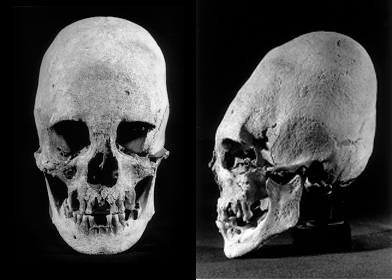
\includegraphics[width=0.70\linewidth]{chast-colebanie-osnov/alani/aw01.png}

\textit{Череп сарматской женщины.}
\end{center} 

Про Сарматов Аланов в популярной научной и околонаучной литературе зачастую умалчивается любопытная штука – некоторые найденные черепа Аланов и Аланок были сильно вытянуты назад (как у многих «каменных баб»). Ученые поясняют это «искусственной деформацией» без каких-либо оснований для такого утверждения. Просто решили, что у людей таких черепов быть не может, у всех должны быть, видите ли, головы более круглые.

А ведь потомки сих Аланок, тоже с вытянутыми головами, видны на портретах жителей Украины и окрестностей за 17-18 века. Тоже искусственная деформация?

Вытянутые, длинные черепа Аланов находят всюду, где обитала эта ветвь Сарматов – в нынешней Франции, Австрии, на Кавказе, Киевщине\footnote{Подобный череп обнаружен в 19 веке в кургане под Уманью, у фермы Марьянки. Однако захоронение относится ко времени, предшествующему Скифам и Сарматам, а также «трипольцам». Значит, люди с подобными черепами обитали на Киевщине с незапамятных времен.}. Археологи находят эти черепа и повторяют – искусственная деформация. 

%А ветвь аланов была большая и могучая, на много отростков – даже до Пакистана дотянулась, где поныне живет народ Калаш (Калаша). А может, калаши и не ветвь, а основа, кто знает? Хотя калашей осталось всего около 5000, они поныне сохраняют свои облик, обычаи и верования, отличные от соседних народов. Выглядят многие калаши своеобразно – я бы сказал, как славяне.

%Конечно, не у всех Аланов были вытянутые черепа, но кстати вытянутых и много, причем с остатками рыжеватых волос, нашел археолог Хулио Сесар Тельо в 1928 году в перуанской пустыне Паракас. И как обычно – сторонники инопланетной теории НЛО понимающе кивают головой, а ученые твердят об «искусственной деформации». 

А ведь довольно сравнить древние, гармонично сложенные вытянутые черепа и черепа в самом деле искусственно измененные, у разных африканских племен – огромная разница. Да и не только у африканских – во Франции этим занимались даже в 19 веке. Верно, подражали давним Аланам, для некоторых представителей которых такие черепа были прирожденной нормой.

Часть найденных в Европе вытянутых черепов археологи относят к Хуннам. Такие же черепа, только одни наука называет аланскими, другие – хуннскими. И про Хуннов тоже говорит – это искусственная деформация черепа! А когда по черепу воссоздают облик, то Хуннам рисуют узкие глаза – мол, монголоиды, а Аланам – пошире. Или лепят подобное из гипса.
 
Но меня занесло в сторону.

Пехоте Тавроскифов у Льва Диакона несколько противоречат конные Роксоланы у Тацита, ибо Тацит, говоря о Роксоланах как о народе, произошедшем от Сарматов (Rhoxolani, Sarmatica gens), описывает их как замечательных в конном бою, и беспомощных в пешем – так, по крайней мере, было, когда Роксоланы вторглись в Мисию во время Оттона и Вителлия. А по всем прикидкам Роксоланы и Тавроскифы один народ.

Но всё зависело от времени и места. Воевавшие с римлянами Сарматы были с головы до ног защищены кольчугой, в кольчуги же одевали и лошадей, покрывая глаза их продырявленными кружочками. Затем мы видим сарматских воительниц и воинов в кожаных латах с металлическими пластинами. Что до конницы, то если сведения Константина Багрянородного верны и Росы покупали лошадей у Печенегов, значит сами были в этом деле не очень-то. Может и Роксоланы – Росы, смешанные с Аланами – тоже не шибко делали ставку на конницу, хотя в летописях есть упоминания о ней, причем в непосредственной связи с князьями Вещим Олегом, Игорем и Святославом. 

Ученые относят Аланов к иранозычным. Это поспешный и слишком общий вывод, верный однако применительно к Аланам, обитавшим около Кавказа и смешавшимся с Иранцами. Но те Аланы, что жили по Днепру, были Славянами со славянским языком. Доказательство очень простое.

Мы знаем из летописей, что здесь жил славянский народ, именуемый Поляне. Довольно отбросить «п» и получить Оляне, те же Алане. Только так могло образоваться название «Роксоланы». Ибо Росы соединились с Аланами. А вспомним каневского Алана по имени Михей!

Более того, доводом для отождествления Аланов и Полян, помимо совмещения по месту и времени, служат былины. В них встречаются женщины-воительницы, именуемые «поляницы». На Украине это слово сохранилось в именовании пшеничного хлеба.

Былины порой освещают седые времена с фотографической точностью, беда лишь в том, что нынешние представления о седых временах совсем другие, и былинная правда воспринимается сказкой.

Верны былины в географии, они знают, например, киевскую речку Почайну под именем Пучайки или Пучай-реки. Былины же именуют Илью Муромца – казаком. Подобно Нартам, старинному богатырскому народу из преданий Осетинов, наши богатыри смотрят вдаль через подзорные трубы. Когда какой-нибудь богатырь приезжает, скажем, к черниговскому князю, тот спрашивает – ты коей земли, коей орды будешь?

Едет Добрыня Никитич в чистом полюшке, встречает поляницу удалую, Настасью дочь Никуличну, и лупит ее в голову\cite{gilder01}: 

\settowidth{\versewidth}{«Думала же, русскии комарики покусывают,} 
\begin{verse}[\versewidth]
На кони сидит же поляница, сворухнуласе\\
И назад же поляница оглянуласе,\\
Говорит же поляница да удалая:\\
«Думала же, русскии комарики покусывают,\\
Ажно русскии богатыри пощалкивают!».\\
Ухватила тут Добрыню за желты кудри,\\
Сдернула Добрынюшку с коня долой\\
А спустила тут Добрыню во глубок мешок,\\
А во тот мешок да тут во кожаной,\\
А повезе же ейный было добрый конь,\\
А повезе же он да по чисту полю.
\end{verse}

Далее конь разговаривает с поляницей – такие же говорящие лошади постоянны в преданиях Осетинов про Нартов.

Поляницы в былинах – не редкая диковинка, а постоянная героиня. Более того, в былине про Ставра сказано:

\settowidth{\versewidth}{Солнышко Владимир князь стольнё-киевской} 
\begin{verse}[\versewidth]
Солнышко Владимир князь стольнё-киевской\\
Задернул он почестный пир\\
На всих князей, на бояра,\\
На всих могучиих богатырей,\\
На всих поляниц да удалыих.\\
Соезжалися на почестный пир\\
Вси князи и вси бояра,\\
Вси могучии богатыри,\\
Вси поляницы удалыи.
\end{verse}

Знали сказители и Роксоланов – в былине «Соловей Будимирович» этот Соловей, вернувшись в Киев с моря Черного, призывает свою дружину – скидывайте с себя кожанки лосиные, надевайте кафтаны роскурлань-сукна! Былины помещают в наше Подолье некую Марью лебедь белую, подолянку да королевичну, русскую красавицу, по всем повадкам – сарматскую воительницу.

Всё найдется в былинах – распри со славянской тогда Литвой, странные отношения с Ордой, Батый (Батыга), какие как брались дани, какие одежды носились. Спелись в былинах исконно скифские и сарматские земли – Днепр и Дон, как небо отражается в реке, так в былине отразилось аланское прошлое Киевщины и язык старославянский, тот самый «церковный»\footnote{Александр Гильфердинг записал эту былину в Пудоге в 1871 году от крестьянина Никифора Прохорова, 51 года возраста, перенявшего былины от отца своего.}:

\settowidth{\versewidth}{А не стрели-тко ты меня Непры королевичной.} 
\begin{verse}[\versewidth]
Как тот ли этот князь стольне-киевской\\
А сделал он задернул свой почёстный пир.\\
Как вси-то к ему на пир собиралиси,\\
Вси там на пиру наедалися,\\
Как вси там на пиру напивалися,\\
Стали там оны вси пьянёшеньки,\\
А стали вси оны веселешенки,\\
Князи вси бояра-то русийскии,\\
А тыи-то могучи вси бог\'атыри,\\
Как вси-то они ведь там расхвастались.\\
Как тут была межу има\\
А тая эта Н\'епра королевична.\\
Как-то тая Непра королевична\\
Как говорит промолвит таково слово:\\
«А нету зде стрельцов добрых молодцов\\
Противо меня Непры королевичной!\\
Силою да нету ухваткою\\
Против стараго каз\'ака Ильи Муромца,\\
А красотою еще было угожеством\\
Противо ведь Михайлы П\'отыка Иванова,\\
А тишиною говорить смиреньицом\\
Противо Добрынюшки Микитица,\\
А нету-то видь еще богачеством\\
Против-то ведь Дюка Степанова,\\
А нету-то да ведь смелостью\\
Противо смелаго Алешеньки Поповича,\\
Поступкой походкою пощапкою\footnote{Щегольство.}\\
Противо-то Чурилки щапа Плёнкова».\\
Сама она еще не спохвалила\\
А тихаго ведь Дона-то сына Иванова,\\
А своёго-то мужа любимого.\\
Как тихий тут Дон сын Иванович \\
А говорит промолвит таково слово:\\
«Ай же ты да Непра королевична!\\
Когда же ты охвоча-то была удалая\\
Стрелять-то было стрелочок каленыих,\\
Пойдём-ко мы с тобой на чисто поле,\\
Станем стрелять стрелочок каленыих,\\
Который ведь стрелять видняе-то?»\\
Как тут-то тая Непра королевична\\
Взимет тут-то ножичок булатныи,\\
Как тое-то колечушко серебряно,\\
Относит что за версту за мерную,\\
Натянула тут она свой да тугой лук\\
А клала ёна стрелочку каленую,\\
Стрелила тут за версту за мерную,\\
Попадала в колечко-то серебряно,\\
И росколола ёна стрелочку равным равно,\\
Да равным то равно стрелку на двое.\\
А клали половинки на весы они,\\
Никоя никоёй не перетягивать.\\
Как тихий тут Дон сын Иванович,\\
Розгорелось ёго сердце богатырское,\\
Как скоро натянул свой он тугой лук,\\
Кладывает стрелочку каленую.\\
Как начал тут Дон сын Иванович.\\
Начал он стрелочкой помахивать\\
А начал ведь-то сам выговаривать:\\
«Ай же ты моя любима калена стрела!\\
Пади же ты не на воду, не на землю,\\
А ты пади ко Непры королевичной,\\
А ты пади же ей во белую грудь».\\
Как тут-то тая Непра королевична\\
Как тут-то ведь она да прослезиласи\\
А тут-то ведь она порасплакалась:\\
«Ах тихий ты Дон сын Иванович!\\
А не стрели-тко ты меня Непры королевичной.\\
Да несу я ти сына любимого,\\
А по колен-то ноженьки во серебри,\\
А по локоть-то рученьки во золоти,\\
А по косицам текут будто звездышки,\\
На зади-то возсият будто светел месяц,\\
Впереди-то как будто солнышко».\\
Как розгорелось ёго сердце богатырское,\\
А ничего тут он ведь не последовал.\\
Как скоро он стрелил ю во белую грудь,\\
Как пала тут она на сыру землю,\\
Облилась она кровью тут горючею.\\
Как тихий тут Дон сын Иванович\\
Взимает он ножищо тут кинжалищо, – \\
Ино ль то ведь еще правда ль есть?\\
Пластал-то он ведь ей да белую грудь.\\
Как было-то ведь тут да до правды бы:\\
Засиян-то ведь во чреви тот сын-то был,\\
По колен-то ноженьки во с\'еребри,\\
По лок\'оть-то рученьки во золоти,\\
Назади просвичать будто свитёл месяц,\\
Впереди еще как там солнышко.\\
Как взял это ножищо он кинжалищо,\\
Становил он-то ножик ведь супротив себя,\\
А становил он ножик, выговаривал:\\
«Да куды пала головка белой лебеди,\\
А тут пади головушка сера гуся».\\
Пал он на ножищо тут кинжалищо,\\
Да тут-то им пришла е горьк\'ая смерть.\\
Как от их-то от крови от крестьянскии\footnote{Христианской.},\\
От крестьянскии крови безнапрасныи,\\
Как протекала тут да Непра река.\\
В глубину река двадцати сажон,\\
А в ширину река сороки сажен.\\
Только-то ведь Донушку славу поют,\\
А той ли этой Непры королевичной.\\
Тут-то их да жительство решилоси.\\
\end{verse}

И складывались эти былины да во времечко, когда Сарматы, коих всех ученые объявили «ираноязычными племенами» и отодвинули далеко в прошлое, говорили одним языком с нашими богатырями, сиживали с ними за одним столом, и были если не всем здешним народом, то доброй его половиной. И если «поляница» – это Аланка, то былинный казак – это «ас» или «аз», такой же Алан. Поныне в Ближних пещерах лежат останки, приписываемые «старому казаку» Илье Муромцу.

Это странные останки. Их ведь изучали, во время Перестройки, и пришли к выводу, что Илья вообще не мог ходить из-за некоего заболевания позвоночника (я не мог найти подробности). Рост Муромца был 177 сантиметров. Необычно толстые кости черепа – лобные, теменные, затылочные. Выдержат, по словам проводившего исследование судмедэксперта Сергея Никитина, удар молотком, от которого у другого человека будет черепно-мозговая травма, вдавленный перелом.

Такие же необыкновенно большие и кисти рук. Более мощные запястья и ключицы.

Всё это некоторые ученые списывают на болезнь. Кроме того, хотя по былинам Илья и просидел сиднем 33 года, но потом в подвижности давал фору многим, значит таки ходил. Почему бы не предположить, что Илья просто отличался от людей обычного биологического вида? Возможно, такое строение тела было для богатырей нормой? Не от болести у Илюши крепки костушки, а богатырское строение таковское. Настоящая боевая машина. Думаю, у других богатырей было подобное.

Муромец скончался в возрасте 40-45 лет. При осмотре останков, у него обнаружено несколько переломов ребер, правой ключицы, проникающее ранение левой руки, сквозное ранение грудной клетки острым предметом – предполагают, от сего и помер.

Что же, вдоволь наговорившись про Аланов – но я к ним еще вернусь – приступлю к тому, что послужило заделом главы – городам Амадоку и Азагориуму. Памятуя о разных народах, скифских да сарматских, сможем более толково рассмотреть птолемееву карту, точнее ее кусок. 

Правильнее говорить, однако, «карта по Птолемею». Клавдий Птолемей был математиком, астрономом, астрологом, географом из Александрии, что в Египте. Общепринято считать, будто Птолемей жил в первом веке нашей эры, хотя труды его известны Арабам только вроде бы с девятого века, а основная его работа по географии – собственно «География» – всплывает в Италии почему-то лишь в начале 15 века и в латинском переводе, хотя по источникам (я не проверял) греческие списки прослеживаются с 13 века. Веком ранее начинают прослеживаться опять же латинские переводы другого сочинения Птолемея, астрономического «Альмагеста», причем выполненные с арабского. 

Выходит, что две известнейшие работы Птолемея стали известны посмертно спустя почти десять веков после их написания, если придерживаться традиционной хронологии, в которой возможны любые чудеса. Более правдоподобным мне кажется, что возникновение списков (прослеживаемых по источникам) с этих работ и есть примерное время написания подлинников. И Птолемей жил незадолго (в пределах нескольких веков) до пришествия на Киевщину Вещего Олега.

Карты, нарисованные рукой Птолемея, не сохранились. Ныне известны лишь составленные «по Птолемею», и я буду использовать карту из рукописного издания 1480 года, так называемого «Уилтонского кодекса».

Немного о самой «Географии». В основу своего труда Птолемей взял работу Марина из Тира (Μαρίνος ο Τύριος), которая не дошла до нас. Другое упоминание Марина встречаем только у арабского географа аль Масуди, который отзывался о картах Марина как о превосходящих карты Птолемея. Правда, сам Птолемей говорит, что Марин карту начертить не успел, а оставил только текстовое описание.

Именно Марин первым из известных нам картографов ввел координатную систему по ширине и долготе. Единицами измерения в ней ввел градусы, а с одним градусом соотнес примерно 500 стадий. По странам составлялись списки городов, городам назначались координаты. Потом, исходя из этих текстовых описаний и уточняя положение по определенным формулам, следовало чертить карту, причем надо было сферическую поверхность (Греки знали, что Земля круглая) перенести на плоскую.

Но Птолемей пишет, что по данным Марина верную карту начертить невозможно, вдобавок Марин дает не\-полные координаты – то приводит одни лишь широты, то долготы. «География» Птолемея, таким образом, это надстройка над работой Марина, с многочисленными исправлениями и дополнениями (из других источников), которые позволяют таки начертить по текстовому описанию приемлемую плоскую карту. 

Но многие города так и остались с «одной координатой». По карте видно, что знаменитые Амадок и Азагориум, а ниже Сарон и Ниоссон, лежат на одной долготе. Подобные «однодолготные» города есть и восточнее вдоль Хипаниса.

Возникает вопрос, а как же заданы координаты рек? Ведь река – не единичная точка на карте, но совокупность точек. Если записывать такую последовательность точек, составляющих реку, то, допустим, через определенные промежутки. И затем, перенеся эти точки на карту, соединить их линией. Так мы получим примерные очертания реки.

Однако «География» Птолемея не содержит таких данных по рекам. Даются сведения, что река такая-то протекает в такой-то местности. И указаны координаты ее устья и, если известны – истока. Следовательно, реки на картах, составленных по Птолемею, изображены условно от точки истока до точки устья.

«Дополненные» координаты для Азагориума и Амадока – хотя я не исключаю, что они в самом деле лежали на одной долготе – и примерные изображения рек на карте Птолемея не дают представления о том, на каком берегу находились эти города и даже как далеко они отстояли от берега.

Вот города по берегам Днепра из труда Птолемея:

\begin{longtable}{l|l}
Город & Координаты\\ \hline
Азагорион (Азаргариан) & 56° 30'  50° 40'\\
Амадока & 56°(30') 50° 30'\\
Сарон & 56° 50° 15' (45')\\
Серимон & 57° 50°\\
Метрополис & 56° 30' 49° 30'\\
Олбия (Борисфенис) & 57° 49°\\
\end{longtable}

%Город & Координаты\\% \hline
%Азагорион (Азаргариан) 56° 30'  50° 40'\\
%Амадока 56°(30') 50° 30'\\
%Сарон 56° 50° 15' (45')\\
%Серимон 57° 50°\\
%Метрополис 56° 30' 49° 30'\\
%Олбия (Борисфенис) 57° 49°\\

Можно ли перевести их координаты в одну из используемых ныне картографических проекций? Ученые занимаются этим давно и приходят к противоречивым выводам.

Кроме координат городов, Птолемей дает примерные координаты гор (в качестве единичных точек) и описывает, где какие народы живут – основываясь невесть на чьих данных.%Роксоланы у Птолемея помещены на берег Азовского моря, а севернее их – Амаксобии и Аланы.

Давайте наконец поглядим на карту, памятуя, что ее начертил не Птолемей. Она составлена кем-то по текстовому описанию, сделанному Птолемеем, что приводил координаты, рассказывал, какие где живут народы и так далее. Порассуждаем над картой, хотя вернее было бы рассуждать над текстом Птолемея. Карта всё же нагляднее, но искажена переосмыслением составителя карты. 

\begin{center}
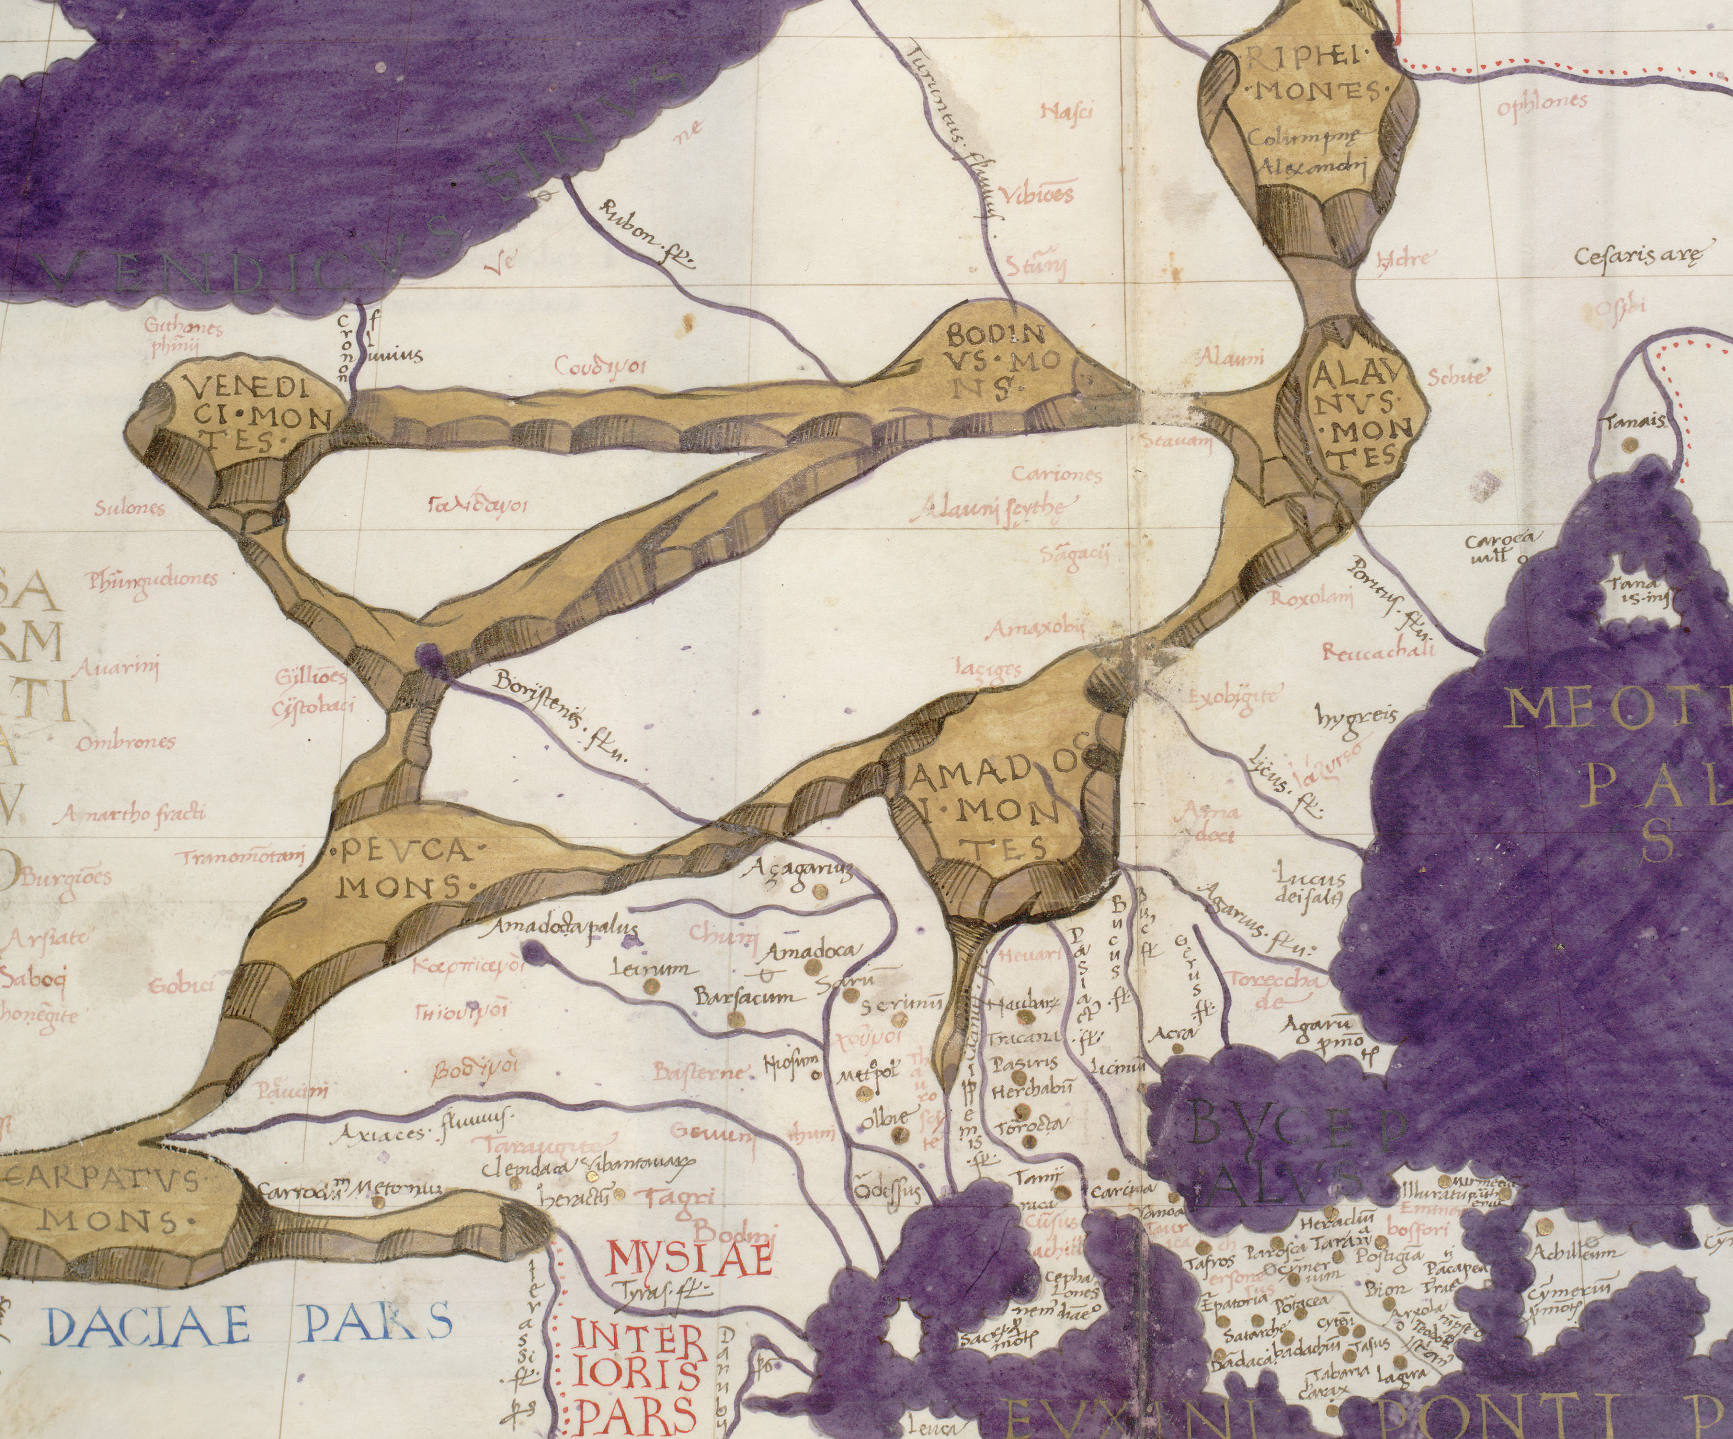
\includegraphics[width=\linewidth]{chast-colebanie-osnov/alani/ptol.jpg}
\end{center}

Многие исследователи не видят разницы между сочинением Птолемея и «его» картами, строя на основе последних умозаключения. В то время как сии карты могут служить лишь для поверхностного суждения о сведениях, изложенных Птолемеем. Таким ли будет суждение собственное, вынесенное при близком знакомстве с «Географией»?  

Сразу бросается в глаза, что карта ориентирована не на привычный нам север, а со смещением, как если бы взять современную карту и повернуть ее против часовой стрелки. А ведь Греки отлично разбирались в сторонах света. Здесь карта не просто от фонаря нарисована, но с координатной сеткой, где меридианы (параллельные линии, от нулевой из которых отсчитываются долготы) ведут к полюсам.

Выходит, что полюса на картах, составленных по Птолемею, отличны от современных нам. Я не буду здесь делать из этого выводы. Но далее, пользуясь сторонами света в разговоре об этой карте, применяю ту систему координат и те полюса, которые присущи именно этой карте.

В правом верхнем углу – устье Tanais, Дона. Он впадает в Азовское море (Мэотийское озеро).

Левее – Alanus Montes, Аланские горы. 

Горная цепь тянется от Аланских гор вниз-налево к Amadok Montes, горам Амадок. Это примерно холмы вдоль Северского Донца, Донецкий кряж.

К северу от них на карте подписаны местные народы – кроме прочих Аланы Скифы, Амаксобии\footnote{Корень «άμαξό», амаксо, значит «правящий повозкой».}.

Но пространство западнее, левее этих народов – пусто. Населено ли оно ими, или нет – неясно. От гор Амадок горная цепь идет дальше налево, как понимаю, как запад, и пересекает наш Днепр – на карте обозначен как Борисфен, Borisfenis flu.

Ниже пересечения Днепра горами, первым, на правому берегу, идет город Азагориум. Ниже, через некую реку – город Амадока. По левому берегу южнее – Сару.

Ниже Сары, в Днепр с правого берега вливается некий приток, берущий начало в озере Амадок. По его левому берегу лежат города Лемум и Барсакум. Южнее устья сего притока расположен город Ниосум.

По левому берегу Днепра далее – город Метрополь, затем Днепр раздваивается, впадает в Черное море, и между устьями Днепра видно «Одэссус». Этот Метрополь, невзирая на координаты, некоторые ученые соотносят с Киевом. Ольвия помещена к востоку от второго рукава, весьма глубоко в материке.

Также на карте есть горы Бодинов (небось геродотовы Будины). А возле Аланских гор живут Аланы. Горы Амадоков и город Амадока явно связаны. Можно предположить существование одноименного народа – Амадоков. Так и есть – они показаны южнее гор Амадок. От города Амадоки этих Амадоков отделяют горы.

Местность возле Азагориума и Амадоки, по карте, населяют Кхуни – и сложно усмотреть в этом нечто иное, нежели Хуннов или Гуннов. А ведь наука говорит, что Птолемей жил в первом веке нашей эры! И эта же наука говорит, что Хунны проявили себя в пятом веке, во всяком случае тогда они попали в Европу! Что же, по общепринятой науке, Птолемей – великий провидец? Нет, это еще одно подтверждение ошибочности хронологии, которой придерживаются ученые.

Я попробовал умозрительно наложить карту по Птолемею на современную, учитывая, что каждая горная цепь на древней карте была задана точкой, и по неким соображениям дорисована. Над Азовским морем получаются горы Аланские и Амадокские. Это возможно современный Донецкий кряж, проходящий между Луганском и Донецком и затем сворачивающий (при современном полюсе) на юго-запад к Мариуполю и оттуда еще западнее, почти к излучине Днепра ниже Запорожья.

На карте по Птолемею мы видим, что некая возвышенность, горный рукав, пересекает Борисфен и тянется к горам Певка, к югу от которых лежит озеро Амадок (Amadoc palus).

Попытаемся пробить Певку и Амадок по древним источникам. Не горы, но остров Певка и народ Певкины помещаются Греками в устье Дуная. Название острова в переводе значит Сосновый от растущих на нем сосен. По Страбону, населяющие его Певкины произошли от народа Бастарнов. Остров сей был известен еще во времена Александра Македонского. Арриан в «Походе Александра» упоминает крутые берега острова, а вдоль – речной рукав с течением столь сильным, что невозможно стать на якорь.

Ныне в устье Дуная нет ни огромного острова с остатками города, ни стремительного рукава. Напротив устья, в море, находятся жалкие остатки большого некогда острова с похожим на Певку именем – Левка, он же остров Ахилла, теперь его величают Змеиным.

Теперь про Амадоков. Ничего про них, кроме географических названий вроде гор Амадоков, города Амадоки, озера Амадоки я не нашел.

Зачем всё это, если, казалось бы, Птолемеем даны координаты, бери да переводи в современные. Но это тупиковый вариант, ибо поныне неясно, как именно переводить. Этим занимается множество исследователей, и у них выходит разное. И нигде в известных мне попытках такого перевода не учитывается иное положение полюсов. 

А я не обладаю достаточными знаниями, чтобы взяться за дело, но даже если бы мне удалось совершить точный, а не умозрительный перенос карты Птолемея (во многом весьма условной) в какую-нибудь современную проекцию, что бы я получил? Мне нужно, во-первых, русло Днепра. У Птолемея русло задано начальной и конечной точкой. Координаты городов Амадоки и Азагориума с их одинаковой долготой вызывают у меня подозрение. 

Так что за возвышенность или горная цепь между горами Певка и Амадоки, пересекающая Днепр?Подобное пересечение ныне известно лишь в месте затопленных порогов около Запорожья. Исходя из этого, Амадока и Азагориум лежат тоже ниже порогов, а никак не на Киевщине. Из древних источников нигде, кроме «Географии» Птолемея, эти два города не упомянуты.

Если горы Амадок это Донецкая возвышенность, то западнее ее лежит Приазовская возвышенность, что несколько уходит от порогов южнее. А горами Певка могут быть холмы к западу и северу от Кировограда.

Одним словом, если возвышенность через Днепр на карте по Птолемею не выдумка, то ее придется пояснить одним – изменением рельефа местности. Например, горная гряда была занесены слоем грунта таким образом, что превратилась почти в равнину.

Что до Киевщины, Полтавщины и Черниговщины, то они на карте по Птолемею лежат в пустом месте между вышеупомянутой загадочной возвышенностью через Днепр и следующей возвышенностью к северу, возможно Валдайской, где начинается Днепр. И Птолемей не знает там ничего, кроме «пустыни», в которой живут Скифы Аланы и несколько других народов.

А может статься, это всё другие горы, сгинувшие, и сопоставление с современными возвышенностями – ошибочно. Ведь не существует более огромного озера Амадоки, которое упорно держалось веками на множестве старинных карт.

Теперь отрешимся от того, что нарисовано на карте. Это не карта Птолемея, но составлена по тексту его «Географии». 

Сравниваю с текстом. Данные, перенесенные на карту, приведены в третьей книге, главе пятой. Всё это, по Птолемею – Сарматия. Он пишет, в параграфе 19, что по всему берегу Мэотиды живут Иазыги (Ιαζυγες) и Роксоланы (Ρωξολανοι). А за ними, вглубь страны – Амаксобии (Αμαξοβιοι) и Аланы Скифы (Αλαυνοι Σκυθαι). Описание места их жительства размыто, однако по нашим летописям, тоже размытым, примерно те места населяли Поляне, славянский народ. Они же, выходит, те, кто у Птолемея – Аланы, скифский народ. 

Однако Языги (Ассы) считаются другим названием Аланов. Может, прав Птолемей, разделяя их. А может, перечень народонаселения в «Географии» сводный, туда выписывались данные из разных источников, а составитель по неведению не сопоставил Ассов с Языгами и поместил их как два отдельных народа.

Аланы неразрывно связаны с рекой Борисфен – в поэме римского императора Адриана приведено имя коня Юлия Цезаря – Борисфен Аланский.

Что же случилось с Аланами? Они растворились в населении одних мест и составили основу населения других. На Киевщине Поляне-Алане – проживали до прихода Вещего Олега с Русами и неясно, в какой степени произошло смешивание, а с учетом многочисленных разорений Киева да окрестностей, и последующих волн заселения, можно предположить, что в некоторых современных киевлянах есть доля аланской крови, однако никто не является Аланом полностью. 

От Аланов остались также названия стран и местностей, где они проживали – при этом сами Аланы могли, опять же, сгинуть оттуда или раствориться, либо растворить. 

Земли Польши в давнее время звались Полонией, а на старинных картах между Полонией и Молдавией лежит Руссия (не Киевская Русь и не Московия), а севернее Руссии – Волиния, в чьем имени тоже угадывается аланское созвучие. Также и другие Аланы – Асы, Язы, Осы – оставили след свой в Осетии, Азербайджане, в имени Азовского моря, возможно и современной Албании. Примечательно, что на родном языке Шотландцев – гаэльском – Шотландия называется Алба или Албания. А Scotland она называется от Ск\'отов (Скоттов) – ряд давних источников возводит название к Скоте, дочери фараона Сингриса, современнице Моисея и жене предводителя некоего возможно скифского народа, который двинулся затем из Египта и, после скитаний, осел в Ирландии. Кстати в нынешней Шотландии существует местность под названием Росс.

Но это уже о Росах, про них мы поговорим позже, они ускользают, тоже всюду оставляя свои следы, причем даже в Азии, Малой и обычной. Да и Скифы.

В устье Иордана лежит город Beit Shean (Бейт Шеан), где туристам показывают развалины древнего города – остатки зданий с колоннами, громадного амфитеатра на 7 тысяч зрителей, бассейнов, общественных бань. Это прежний город Скифов, Скифополис, дважды упомянутый еще в Ветхом Завете. Один раз – когда после странствий по пустыне, сыны Израилевы начинают уничтожать или подчинять себе города. Второй раз о Скифополисе сказано в Книге Иудифь. В ней же, Олоферн – военачальник Ассирийского царя Навуходоносора – «разграбил всех сынов Рассиса», перемещаясь где-то возле Киликии.

А возьмите название другого города – Иерусалим, в давних источниках именуемый Русалим и Урусалим. Я не поднимаю тут тему возможного родства Славян и некоторых Евреев – хотя можно почитать работы Пола Векслера, например «Ашкеназийские евреи: славянско-тюркский народ в поисках еврейской идентификации» (Paul Wexler The Ashkenazic Jews: A Slavo-Turkic People in Search of a Jewish Identity). Другие исследователи напротив, выводят русских от восточных Евреев, плохо понимая вообще, что значит понятие «русские» (прилагательное, применяемое к народам, попавшим под власть народа, известного как Росы), третьи стараются их всеми силами противопоставить.

Можно взять название любого города и прилагать его то к одному, то к другому. Русалим – еще к русалкам близко, и к русальим дням, русалиям.

Вот Скифополис – более твердая почва для размышлений. Город Скифов. Город в выгодном торговом месте – устье Иордана. Сам по себе, если бы окружающее население было к Скифам враждебно, он бы не возник. Не выстояли бы Скифы. Значит, в том месте, в некоторое время, Скифы могли считаться если не «своими», то дружественными. Возникает вопрос – не было ли среди тамошнего окрестного населения других Скифов? Каково было самоназвание Скифов, населявших Скифополис?

О Скифах в Азии пишет Геродот, касаясь истории Мидийского царства. Сменили один другого три правителя – Дейок, Фраорт, Киаксар. Последний расширил границы владений, покорив Ассирийцев. В это время в Азию явилось войско Скифов, которые гнали Киммерийцев из Европы. Во главе войска стоял царь Скифов по имени Мадий (возможно, Матий – от «мать», так же как Батий – от «батя»), сын Протория. Мидяне пытались дать Скифам отпор, но проиграли – не только в сражении, но и во властвовании над Азией, и Скифы держали последнюю в своих руках еще 28 лет.

После битвы с Мидянами Скифы двинулись на запад, в Палестинскую Сирию, но были остановлены египетским царем Псамметихом, который лично вышел к ним с дарами и договорился про обход его земель. Скифы отправились через и ныне существующий древний город Аскалон, и по некой причине не тронули его. Последующие три десятилетия Скифы брали дани с азийских народов, и грабили их помимо даней, но постепенно были перебиты Мидянами. Те отвоевали некогда подчиненные себе земли назад, кроме оставшегося независимым от них ассирийского Вавилона. Будущий поход персидского царя Дария против Скифов (когда в помощь Скифам пришли Савроматы, Гелоны и Будины) был вызван желанием отомстить за столь длительное былое господство над Персами (Иранцами).

Но может, Скифы или родственный им народ обитали в Азии еще до преследования Киммерийцев?

Посмотрим на карту. Какая страна находилась неподалеку от Скифополиса? Финикия\footnote{Отметим сходство ее названия с Венецией.}. Все ученые знают, кем были финикийцы – семиты, изобрели вдруг свою азбуку, потом ее переняли и расширили Греки, а Кирилл и Мефодий на досуге положили азбуку Греков в основу славянской.

Мне кажется, дело было наоборот. У неких изначальных Скифов и Сарматов был свой алфавит. Они жили, кроме прочего, и в Азии. Финикийцы – ветвь этих Скифов либо Сарматов, мне трудно их различать. Славяне – тоже ветвь Скифов и Сарматов. Поэтому алфавиты Славян и Финикийцев подобны. А Греки?

Проще ответить, если записать Греков в потомков Скифов и Сарматов. В Греции раньше жил народ Пеласги (Πελασγοί). Геродот отмечал, что говорили они на варварском языке. Эллины – на греческом, а вот Пеласги – на варварском. Варварами для Эллинов обычно были Скифы.

Пеласги соединились с Эллинами и другими народами, в том числе темнокожими (о чем свидетельствуют многочисленные монеты и рисунки на посуде\footnote{Судя по тем же рисункам, в давнее время люди сосуществовали с Сатирами, Кентаврами и другими существами, которых наука считает сказочными.}) – так возникли Греки, говорящие на языке Эллинов. Но если Пеласги являлись частью Скифо-Сарматского народа, общности, то понятно, почему у Греков такой же алфавит, как у Славян или у Финикийцев.

А если переплыть из Греции на восток, мы попадем к бывшей Финикии, а также в Палестину. Палестиной эта страна называется от некогда жившего там народа, известного древним Евреям как «Пелистим» (библейские язычники-Филистимляне)\footnote{Про них много рассказано в Ветхом Завете. Например, в Книге Царств, Фелистимляне отобрали у сынов Израиля ковчег со скрижалями, и принялись возить оный по своим городам, никто не хотел у себя его оставлять, ибо местное население покрывалось «болезненными наростами».}. Не надо далеко ходить, чтобы усмотреть общую основу у Пеласгов и Пелистима. Они жили и в Греции, и в Палестине. Кто в каком направлении переселялся – дело стороннее.

Город Скифополис находился там, где обитали ветхозаветные Филистимляне.

Всюду Славяне, что ли? Почти. Некий большой народ с более-менее одинаковым языком (отличавшийся говорами) в давнее время населял, кроме прочих народов, Европу и Азию. Части этого народа именовались, в разное время, в разных местах – Скифами, Сарматами, Пеласгами, Славянами, Полянами, Аланами, Асами, вероятно и Хуннами, Готфами – а части всё дробились, какие-то сохраняли величину и язык, какие-то утрачивали общность с родственным народами, роднясь с другими.

Стремление ученых превратить эти, скажем так, славянские народности, в дикарей доходит до крайности. Письменности их лишили, лишают и ювелирного искусства. 

Всем известно про «золото Скифов» – золотые украшения, равных которым трудно сыскать и поныне. Их отличительные черты – определенный стиль, названный «скифским», насыщенность бытовыми сценами, животными, да сюжетами якобы из мифологии Греков. Наука утверждает – Скифы заказывали вещи из золота у Греков. Мол, только Греки были мастерами в этом деле!
  
Найдут в скифском кургане золотые кругляши с портретами – говорят, что это не монеты, но бляхи. Вестимо, зачем «диким» Скифам монеты? А что значит «бляхи», каково их предназначение – между пальцами крутить? Не понимаю. Бляхи. 

Или отыщут шлем и называют его «греческим», хотя точно в таких же шлемах Скифы представлены на древнем литье. Почему женщин со скифских изображений ученые именуют «юношами»? Животных же вроде гриффонов, которые показаны рядом с лошадьми, львами, зайцами и утками считают выдумкой. Стороной обходят и постоянный образ сфинкса в скифских украшениях.

%В Керчи рядом с жилыми домами на улице Братьев Перепелицы находятся остатки кургана – поросший травой долгий пригорок, в котором в конце 19 века нашли выложенный каменными плитами «склеп Деметры», искуссно расписанный фресками. В 1942 году его повердил взрывом гранаты немецкий зольдат. Возведение в 1970-х жилого квартала ухудшило состояние склепа, его стало затапливать грунтовыми водами. Веками стоял посередине погребальной камеры деревянный гроб с останками – всё это разрушилось, едва лишь вытащили его на поверхность.

Ювелирные произведения Скифов донесли до нас и других, помимо гриффонов, неведомых ныне существ, как например эти кошкоподобные звери с пастями, состоящими словно из лепестков, служащих вероятно для заталкивания пищи в рот. Поскольку этот образ повторяется, предположу, что он передает животных, с которыми Скифы так или иначе соприкоснулись.

Поглядим на «кошек»\footnote{Картинки далее – из книги М. И. Артамонова «Сокровища скифских курганов в собрании Государственного Эрмитажа», 1966.}.

\vspace*{\fill}
\begin{center}
\includegraphics[width=\linewidth]{chast-colebanie-osnov/alani/artamonov-mi-1966-030.jpg}
\end{center}
\vspace*{\fill}
\newpage
\vspace*{\fill}
\begin{center}
\includegraphics[width=\linewidth]{chast-colebanie-osnov/alani/artamonov-mi-1966-025.jpg}
\end{center}
\vspace*{\fill}
\newpage

А вот скифский золотой гребень из кургана Чертомлык, вид с одной и другой стороны.

\begin{center}
\includegraphics[width=0.75\linewidth]{chast-colebanie-osnov/alani/greben01.jpg}
\end{center}


\begin{center}
\includegraphics[width=0.75\linewidth]{chast-colebanie-osnov/alani/greben02.jpg}
\end{center}

Обратите внимание на всадника и лошадь. Судя по этому и множеству других изображений, Скифы редко пользовались сёдлами, а кони их были довольно низкорослыми, размером как нынче в Исландии. Кажется, и у других народов такие лошадки в старину были более распространены, о чем свидетельствует искусство. А на рельефах колонны Траяна в Риме, сарматская конница тоже предстают перед нами бесседельной да лишенной шпор.

Седла и стремена появились в землях Украины, вероятно, для удобства не столь умелых, как местные, наездников, коими были пришлые Русы.  Вспомним – они, поселившись с Вещим Олегом в Киеве, покупали лошадей у Печенегов. К этому относится и упомянутый Львом Диаконом упор на пехоту у святославовых Тавроскифов. А быть может, причина иная – другая привычка верховой езды. Кстати, шпоры впервые среди Славян начинают встречаться у прежнего, славянского населения нынешней Австрии только в 8 веке нашей эры, как следует из найденных погребений. 

Вещий Олег, Русы? Исследователи, склонные видеть в них скандинавов, встрепенулись и справедливо могут заметить, что скандинавы таки предпочитали сражаться пешими.

Что же, поговорим о скандинавах.

%Развернем карту, поглядим названия городов Австрии. По большому счету она протиснулась на запад между славянсикми странами, Чехией да Словенией. Так, Алланд. Понятно, от Аланов. Что еще? Еще не совсем онемеченные Цветль, Гаубич, Кримль, Пребихль (от «пребых»)

\chapter{Две Скандинавии}

Птолемей подбросил нам загадку Азагориума и Амадока, однако карта не дала на нее ответ. Мы и далее будем много обращаться к картам и планам. Вообще план это разновидность карты, с увеличенным масштабом и условными обозначениями, в зависимости от назначения. Например, на топографическом плане местности показаны зеленые насаждения, включая породы деревьев, а также здания, высоты и глубины, направление водных потоков. Карты же – более общие, но с координатной сеткой. А план чаще обходится без нее. Иногда грань между картой и планом стёрта.

Самый ранний из уцелевших планов Киева составлен под руководством полковника Ивана Ушакова в 1695 году. Известен общественности по плохому скану, а также хорошим, но упрощенным перерисовкам. В 1986 году подлинник повредили при снятии фотокопии, и архив больше не выдает его даже избранным. Перерисовки есть в двух вариантах, дореволюционные да из советской книжки «Киев во второй половине XVII века» Г. В. Алферовой и В. А. Харламова, 1982 года издания.

Если сравнить план Ушакова с картой земель от Москвы до Малой Азии, выполненной соратником Петра I Яковом Брюсом в 1697 году, что включает в себя все земли современной Украины и смежные с нею, бросается в глаза огромная разница в примененной технологии.

Киеву не повезло с планами. Они зачастую лишены подробностей и обрезаны по окрестностям. Планов, изданных до 1917 года, больше, чем выпущенных в советское время, однако на дореволюционных редко показан левый берег. На общедоступных планах обычно не отображены мелкие переулки да улочки. Либо, на военных планах – отображены, да не подписаны. Современные карты-планы, включая электронные, верны по спутниковым снимкам, однако грешат ошибочными обозначениями местностей.

О планах Киева пока всё. Теперь о картах.

Старинные карты служат подспорьем в изучении сведений из письменных источников. Знание карт, современных этим источникам, позволяет верно понимать, что же хотел сказать сочинитель. Давние карты представляются нам нелепыми и безумными. Кроме того, они переполнены названиями стран, которых давно нет, или которые известны теперь под другими именами и в других пределах.

Так что же такое карта? Это представление географов определенного времени об окружающем мире. Существовали географические и космографические труды с описаниями мира и его населения. К ним прилагались карты, иногда карты выпускались отдельно, либо как наборы – атласы.

Был такой бенедиктинский монах из города Дубровника, Мавро Орбини (Mavro Orbini, 1563-1610). В 1601 вышла его книга на итальянском – «Царство славян» (Regno degli Slavi)\footnote{Существует два русских перевода – 1722 года и 21 века. Старинный вернее, новый полнее.}. Задействовав уйму источников, ея сочинитель причислил к славянам чуть не все народы Евразии.

Орбини дал краткое описание каждого, по его мнению, славянского народа – где живет и чем знаменит. А родиной Славян он вывел  Скандинавию. Ту самую, известную нам, где ныне Швеция и Норвегия. Ее подразумевал и Мавро Орбини. Но ведь он где-то выписал, из некоего источника, происхождение Славян из Скандинавии. Может, в том источнике говорилось совсем о другой Скандинавии?

В 14 веке в Англии имел хождение «Полихроникон» Ранулфа Хиджена\cite{polychro}, рассказывающий об истории и разных странах. Скандинавия там привычная, северная. Но меня зацепили карты, прилагаемые к этому сочинению\footnote{Варианты карт к спискам «Полихроникона» помещены в сборнике Конрада Миллера «Mappaemundi. Die altesten Weltkarten» изданном в 1895 году в Штутгарте.}. Они отличаются от текста книги, и Скандинавия на них – азиатская страна у восточных или северных берегов Черного моря. Ее соседи – Алания (Аланией Хиджен называл земли к северу от Азовского моря, включая Киевщину), Амазония\footnote{Амазония, где жили Амазонки, на множестве карт помещена около Кавказа, у северо-восточного берега Черного моря, южнее Дона и реки Кубань. Возможно, там сейчас республика Адыгея и Ставропольский край.}, Колхида, Рипейские горы, а иногда – Малая Азия с Троей, Лидия, Хиберия. По совокупности можно предположить, что эта Скандинавия лежит примерно около Кавказа.

Не поймите превратно, я не говорю, что так было. Мол, Скандинавия находилась там-то. Я утверждаю иное – Мавро Орбини основывал свое мнение на источниках, в которых, возможно, Скандинавия была помещена возле Черного моря, и неподалеку от Азии в тогдашнем понимании этого слова, а оно двойственно.

Вот карта, прилагаемая к «Полихроникону»:

\begin{center}
\includegraphics[width=\linewidth]{chast-colebanie-osnov/okartah/scand-01.jpg}
\end{center}

Ориентация примерно на восток. Я отметил цветными кружками Аланию (во Внутренней Скифии, Скитии) и Скандинавию. На береговом протяжении между ними – Мэот Палус, ныне Азовское море. Западнее (ниже) Скандинавии, в море – остров Колкос (Colcos), показанный на многих старинных картах и по названию имеющий отношение к Колхиде. Река возле Колкоса, исходя из лежащих у берегов ее стран – Дунай. Напротив Скандинавии, правее – полуостров Малой Азии. Восточнее, выше – Каспийское море (mare Caspium). К западу от Алании – Саксония. Запомним, это важно. Алания же – нынешняя Украина с Польшей.

Я бы отнес сию восточную Скандинавию к разряду диковинных ошибок и прошел мимо, если бы эта «ошибка» не была постоянной составляющей именно на картах к «Полихроникону». Давайте поглядим на другой вариант:

\begin{center}
\includegraphics[width=\linewidth]{chast-colebanie-osnov/okartah/scand-02.jpg}
\end{center}

Скандинавия занимает здесь почти прежнее место у берега Черного моря, чуть сдвинувшись на восток (вверх), остальные границы прежние – Иберия, Амазонки, Мессагеты. Хорошо нарисован Танаис к западу от Скандинавии, а еще западнее – Мэотийское болото. Из карты следует, что Скандинавия находится на восток от Дона, однако выше Малой Азии. Это Кавказ либо Ставропольский край.

На современной карте Грузии, в тридцати километрах на восток от Кутаиси с трудом отыскивается село Сканде (სკანდე)\footnote{42°15'36"N 43°3'11"E}. Чуть севернее его – остатки крепости\footnote{42°16'6"N 43°2'46"E}. Это всё, что осталось от древних города и крепости Сканды (სკანდის ციხე, სკანდა).

На протяжении, быть может, тысячелетий она то разрушалась, то возрождалась, переходила из рук в руки, о ней забывали и вспоминали. Прокопий Кесарийский в «Войне с Персами» пишет, что в Лазике (западная Грузия) обжит лишь северный берег реки Риони, и:

\begin{quotation}
Все селения Лазов находятся здесь, на этой стороне реки, и тут издревле построены ими городки, в том числе самый укрепленный из них Археополь, Севастополь и крепость Питиунт, а у самых границ Ивиров Сканда и Сарапанис.
\end{quotation}

В обозримом по источникам прошлом Скандой владели то Греки, то Персы (Иранцы). Ее разрушил в 14 веке Тамерлан, но уже спустя несколько веков она служила пристанищем грузинской царице Тамаре, захватывалась попеременно то картлийскими, то имертинскими царями. Многократно о Сканде пишет грузинский историк 18 века Вахушти Багратиони в «Истории царства Грузинского».

А вот почитаем выдержку из «Статейного списка посольства в Имеретию 1650-1652 гг., составленного Алексеем Иевлевым»:

\begin{quotation}
И провожали послов до подворей азнауры. А что за столом цари подавали изперед себя послам кушенье, и те ествы прислали цари за послами к Микифору и Олексею на стан. А стоял Александр цар. под городом под Скандою, от города с полверсты; двор его учинен на площеди, на ровном месте поставлены поземные дощатые чердаки.

А город Сканда стоит на горе; каменой, четвероуголен, высок, сажен в десять. По стенам четыре башни а на башнех три пушечки волконейки, небольшие.

Да в городе ж церковь камена, без креста, во имя страстотерпца Георгия; в церкве стенное писмо. Да в церкве ж три образа: всемилостивого Спаса, да пречистые Богородицы, да Георгия страстотерпца; обложены серебром в чекан, позолочены; у спасова образа венец золот, писан мусиею. Да на городовой стене сделана полата болшая на трех житьях; а в верхнем житье лежит царева казна, и что прислано к нему Александру царю от ц-ого в-ва жалованье соболи, и те соболи положены в той же полате. И стерегут того города и казны тюфенчеи. Да в городе ж онбар болшой, деревяной насыпан полон хлеба; да вместо погреба вкопана в землю корчага болшая и налита виноградом на целой год, для осадного времени. А мерою того города около сто двадцать сажен болших.

Да около ж того города обрублено тарасы и насыпано хрящем. А всход к городу один и тот круг; взять приступом никоторыми мерами нельзя, гора каменная, да около обрубу, на той же горе, жилых дворов с тридцать. А иные дворы стоят под горами в стрелбище, и в два, и в полуверсте, и в версте, и боши, врозни, по крепким местом, для приходу воинских людей.

А от столного города Кутатиса до того города до Сканды верст с тридцать. А место пришло низ, ровнедь с долинами, верст на шестьдесят; а поперег от Сканда города до реки до Курлы верст с двадцать и болши. А места жилые, городки, и села, и деревни, и стоят по крепким местом, по речкам. И на том ровном месте многие царевы дворы устроены. А по другую сторону того ровного места, под гурелскими горами, течет река Курла. А течет из гурельские земли промеж гор, и вышла из гор в Олександрову землю, и впала в Реонь реку, от Кутатиса вест с шесть или с сем.
\end{quotation}

Когда крепость опустела – неведомо, равно как её создатели и время постройки. Туристы в Сканду не ходят, а краеведы туда добираются с трудом. Зная про Сканду, думаешь – так ли нелепа Скандинавия на старинных картах? Не являются ли они отголоском времени, когда крепость эта была, возможно, основой одноименной державы?

Что до нынешней Скандинавии, то ее часть в давнее время предстает в источниках то как единый остров Скандия, то несколькими островами, и постепенно обретает новое имя – Скандинавия. Под именем Scandia ее упоминает Птолемей в своей «Географии», для него это три острова: Нериг (давнее самоназвание Норвегии – Нориг), Берги и Думна. 

Сейчас Скандинавия известна как полуостров – но при повышенном уровне воды в океане могла быть цепью островов. С подписью «Скандии» полуостров изображается уже на картах 16 века, например на подробнейшей шведской морской карте Олафа Магнуса за 1530 год.

Языческие боги этой, привычной нам Скандинавии – Асы или Осы во главе с Одином – родом из Азии. Считается, потому и Асы, что от слова «Асия». В преданиях, Асы изначально предстают не богами, но могущественным сообществом людей, вроде Туаха Дэ Дананн. Обожествили их позже. \'Один же был, в некоторое время, просто предводителем Асов, колдуном и провидцем.

По «Саге Инглингов» (Ynglinga saga) из «Круга Земного» Снорри Стурлусона, Асы обитали в стране Асаланд или Асахэйм (Ásaland eða Ásaheimr), что лежит к востоку от реки Танаис, прежде именуемой Танаквисл или Ванаквисл (Tanakvísl eða Vanakvísl), впадающей в Черное море (Svartahafi). Страну в низовье этой реки называли Ваналанд или Ванахэйм, а ее жителей – Ванами. Главный же город в стране Асов – Асгард (Ásgarð). Ваны и Асы поначалу воевали, а после породнились. Ваны научили Асов своему колдовству.

Казалось бы, ясно сказано «Танаис». Но река Дон, с которой отождествляют Танаис, впадает в Азовское, а не Черное мое. Быть может, Снорри подразумевал под Танаисом другую реку, например Истр, Дунай? Но будем пока руководствоваться общепринятым толкованием, что Танаис это Дон.

По одним представлениям древних, Азия отделялась от Европы рекой Танаис. По другим представлениям, Азия – южное побережье Черного моря, известное в некоторые времена как Малая Азия.

В прологе «Младшей Эдды» сказано, что в Азии был город Троя, которой правил Тор, сын Меннона и Троан, дочери царя Приама. Из рода Тора происходил Один. В «Младшей Эдде» Троя отождествляется с Асгардом и помещена в Тыркланд (Tyrkland). А вроде бы известно, что сейчас это Турция. 

Малая Азия – часть Турции. Развалины Трои в ней показывают туристам. Впрочем нигде, кроме некоторых саг, Асгард не сопоставляется с Троей, а по географическому описанию из «Саги Инглингов», как увидим далее, Асгард находится эдак на Кавказе или в Ставропольи. 

В старину вообще многим народам было лестно ставить Троянцев себе в предки. И к сообщениям о сторонах света следует, наверное, тоже относиться  осторожно, памятуя о возможном смещении полюсов.

Я неоднократно сталкивался с тем, что в сагах одним словом именуют разные места. А ежели Тыркланд – это не Турция, а некие земли проживания народа Торков, что кочевал от Каспия до Винницы, Донбасса и Поросья? В самом деле, выходит, к востоку от Дона.

Стурлусон уточняет – Тыркланд лежит к югу от большого горного хребта, что тянется с северо-востока на юго-запад и отделяет Большую Свитьод (Svíþjóð ena Miklu) от других стран. Таким хребтом может быть Урал. Словом Svíþjóð в давних северных языках называли Швецию, а вот Большую Svíþjóð можно сопоставить со Большой Скифией, летописной «Великой Скуфью». Иногда впрочем вместо Большой Свитьод писали просто Свитьод, тогда надо было догадываться по смыслу, о чем идет речь.

Если определять положение Асгарда по «Младшей Эдде» и «Саге Инглингов», полагая Дон Танаисом, то выходит, что Асгард лежал к западу от Дона и южнее Урала. Это же Кавказ и Ставропольский край!

В «Саге Инглингов», Асы из Асгарда идут сперва на запад в Гардарики (Garðaríki, их соотносят с землями Киевской Руси), а затем отправляются на юг в Саксланд. В прологе «Младшей Эдды» про Гардарики ничего не сказано, но после странствий Один и его соратники попадают «на север» в Саксланд. Саксланд это будто север нынешней Германии, Саксония.

Выходит путаница, коль руководствоваться современными знаниями, положением полюса и считать сведения из саги истинными. Однако Саксланд лежит южнее Гардарики в случае, если полюс находится примерно там же, где у Птолемея, и привычную нам карту надо повернуть против часовой стрелки. Лишь тогда можно сказать, что Саксланд – южнее Гардарики.

Припомним карту из «Полихроникона» – Алания лежит рядом с Саксонией. Догадайтесь, что общего между Гардарики и большой Аланией от Бэкона, Хиджена, Исидора? То же, что у Киевской Руси да Роксолании – местность.

%Как бы ни было, родина Асов, по сагам, близка к Черному морю и обозначенному на старинных картах месту Скандинавии! Таким образом азиатская Скандинавия обретает весомую привязку. Значит, следует различать позднейшую «северную» Скандинавию с ранней азиатской. 

А теперь перекинем мостик от северной Скандинавии к восточной. В 50 километрах к западу от крепости Сканды лежит Южная Осетия. Грузины называют Осетинов – Оси. 

Север, Скандинавия, Асы. Восток, Скандинавия, Осы. Они же Асы, Ассы, Аланы.

Веками ученые пытались отыскать корни Осетинов, находя их то в Половцах, то в германских народах, то в семитских, пока в 19 веке не пришли к иранскому происхождению Осетинов, что немудрено по их самоназванию – Ирон, Ир! Но для такого очевидного вывода науке понадобились исследования академика Андрея Шегрена.

А ведь даже глядя на современную карту можно сразу сказать, что Осетия с Ираном – соседи. Вероятно, Осетины – потомки древних Иранцев, Персов, волей времени отмежеванные от большей части бывшей родины, которая простиралась до Осетии во времена царя Кира Великого, а затем Дария Первого. Государство Иран – ближайший по языку и месту жительства сосед Осетии!

Но благодаря работам Миллера и Абаева, наука считает теперь Осетинов потомками Аланов, Аланов потомками Сарматов, Сарматов потомками Скифов. Таким образом Абаев развил обоснование тому, что по иранскому в основе современного языка Осетинов можно достучаться до иранской же основы сарматского и скифского языков.

\begin{center}
\includegraphics[width=0.20\linewidth]{chast-colebanie-osnov/okartah/iron02.pdf}

\textit{Схема примерного происхождения Осетинов по Абаеву.}
\end{center}

«Аланами» на этой схеме я для краткости обозначил цепочку Аланы – Сарматы – Скифы, а «Иранцами» именую жителей Ирана, ибо наука не объясняет, каким образом Скифам передался их язык. Приходится предполагать, подыгрывая науке, что от Иранцев.

В самом деле, Осетины живут ныне там, где раньше обитали Аланы – впрочем Аланы были и в нынешней Чечне, и около Днепра и во Франции да Италии, где поныне остались городки Аллейн, Алагна, Сармато Аландриано (Ландриано), Аллегно, Алано ди Пиаве. Славяне-Вандалы купно с Аланами обитали также в Испании, Галии, да по всей даже той части Европы, которую не считают славянской.

Поскольку Осетины называют себя Ирон, думаю, что народ из Ирана растворил в себе аланское население (не важно, коренное или пришлое), и потомки обоих народов и составляют нынешних Осетинов. Вместо того, чтобы предположить оба народа в «одновременные» предки Осетинов, Абаев сделал эти народы последовательными звеньями цепи происхождения.

Выражу взаимосвязь Иранцев, Аланов и Осетинов так:

\begin{center}
\includegraphics[width=0.50\linewidth]{chast-colebanie-osnov/okartah/iron01.pdf}
\end{center}

Влияние Иранцев оказалось сильнее, что выражается в языке и самоназвании – Ирон.

В обозримом прошлом, в осетинском языке не было слова «Алан», пока его не заимствовали из общекультурной среды. А то, что Аланы – давнее самоназвание Ирон, Абаев вывел следующим образом.
 
В преданиях Осетинов существует загадочное выражение «аллон-биллон»\footnote{Кстати, в чеченской сказке «Черкес Иса и чеченец Иса» упомянуто чудесное существо по имени Алла-Белла, обитавшее в пещере.}. Подобно тому, как в русских сказках Баба Яга принюхивается и подозревает, что здесь пахнет русским духом, так в осетинских людоед-великан отмечает – мол, пахнет аллон-биллоном! Абаев не смог истолковать «биллон», однако «аллон» сопоставил с человеком, который находился рядом с великаном. Значит, человек тот – непременно Алан – решил Абаев. А следовательно, предок Осетинов.

О ком же речь идет в преданиях с «аллон-биллон»? Кого вынюхивал людоед? Он вынюхивал Нартов. 

Нарты – народ, о котором рассказывают Осетины в своих преданиях. Нарты сгинули, их покарал бог за дерзость. Ученые гутарят, что в нартовском эпосе отразились Скифы, а Нарты – предки Осетинов. Но ведь сами Осетины говорят – Нарты все погибли. 

К сожалению, еще мало преданий о Нартах переведено на другие языки. А ведь это культурный пласт, сопоставимый по размаху с греческой и северной мифологией, и в некоторых подробностях удивительно перекликающийся с ирландской.

Связь с Ирландией проявляется во многом.

Ирландия, или, в старину – Ир-лонд, земля Иров\footnote{Произношение «Айрлэнд» – английское, на современном ирландском языке звучание иное – «эйжэ», а как оно звучало в старину, неизвестно, есть давнее написание Ériu. В преданиях так звали дочь Эрнмаса из числа Туаха Дэ Дананн. Другой вариант имени – Эрин, почти как Ирина.}. А как называют себя Осетины? Ирами.

Среди Осетинов и Ирландцев рыжих людей больше, чем среди других народов.

Далее. Когда я еще думал, что все Аланы были ираноязычны, то решил, что Туаха Дэ Дананн (Tuatha Dé Danann) можно перевести просто – народы богини Реки, толкуя «Дану» как производное от иранского корня «дон» или «дан».

Правда, в Ирландии не знали богиню Дану. Слово «Дану» вообще придумано учеными, они сочли, что «Danann» это склоненное в притяжательном падеже имя Danu. Мол, чьи народы? Danann. Tuath(а) значит народ(ы), De – божество.% Вместе произносится как «туаха дэ данан», где «дэ» размытое, в нем слышится «ч». 

А если «дэ даннан» – подражание другим словам либо искаженная их передача? В преданиях Осетинов о Нартах важнейшую роль играет чародейка, воительница и советчица по имени Сат\'ана. Я сам не люблю игру с буквами, но «дэдананн» c заменой второй «д» на «т» может звучать как «тэтананн» или «сэтананн».

Сатана – богиня или полубогиня, росшая не по дням, а по часам – за месяц как за год. Это свойство, в преданиях, присуще тем, в ком течет нечеловеческая кровь. Сатана умеет принимать множество образов – являться старухой или молодой\footnote{В 13 веке шотландец Томас Лермонт (Thomas Learmonth the Rhymer) по прозвищу Рифмач (возможно, Михаил Лермонтов – из его рода), провидец, побывал в мире Эльфов, Элфхэйме. Тамошняя королева Фэйри обладала способностью менять свой возраст с молодого на старческий. Три дня прожил Лермонт среди чудесного народа, семь лет прошло в нашем мире. Пробыв некоторое время с людьми, он вернулся в Элфхэйм. Общение с народом Фэйри и королевой Фэйри хорошо освещено в документах из шотландских, 15-18 веков, судилищ над ведьмами. За такое общение, действительное или мнимое, людям со стороны людей же грозили пытки и сожжение заживо. Скиф Анахарсис на вопрос, что самое опасное для человека, отвечал – сам человек.}, понимает птичий язык, управляет погодой, о событиях в мире знает, глядя в некое «небесное зеркало». В сказаниях Сатану описывают как «неба коварство, земли колдовство». 

%По Геродоту, родоначальником скифов был некий Таргитаос: «Родители его были, как говорят, Зевс и дочь реки Борисфен». А в нартовском эпосе, Сатана – дочь Уастырджи

Возможно, Туаха Дэ Дананн следует толковать как «народ Сат\'аны»?

Героические предания Осетинов порой сходны с ирландскими. Часто сравнивают повествования о Сослане (Осетия) и Кухулине (Ирландия). Среди общих подробностей: у Сослана в каждом глазу по два зрачка, у Кухулина четыре в одном, три в другом. Кухулин гибнет потому, что его колесницу зачаровала отвергнутая им богиня войны, призрачная королева Морриган. Отвергнутая богиня же посылает на Сослана самоходную повозку Колесо Ойнона (Балсага, Малсага, Барсага). 

Серебряная рука короля из Анналов Ирландии – и осетинский богатырь Сослан, с телом из черного булата и железными ногами, а также металлический Батраз, столь могущественный, что вступил в распрю с жителями неба и был убит богом при помощи Колеса Балсага. По другому варианту, его расстреляли Елиаты, подлетев в облаке, которое рассеивалось, когда Батраз стрелял в ответ. Батраз раскалился и упал, и ему нечем было охладиться. Он долго лежал. Никто не мог приближаться, умирали, даже противники, жители неба – Зэды и Дуаги.

Не от Нартов ли пошли Туаха Дэ Дананн и обожествленные Асы? Кто такие Нарты в представлении Осетинов? Откроем второй том трехтомника «Нарты»\cite{narty01}. Про народы былых времен сказано:

\begin{quotation}
1. О гумирах\\

Гумиры были огромными, сильными, но глупыми людьми. Они не понимали, что от огня можно отодвинуться, и прикрывали себе лица [кусками] сланца или дерева. Однажды они увидели, как собака все дальше отползала от костра по мере того, как он разгорался. Так гумиры научились оберегать себя от огня.\\

2. Нарты\\

До нартов [на земле] жили гумиры, топоров у них не было, деревья они вырывали руками. Потом появились уаиги – крупные, могучие люди. Вслед за ними [появился] нартовский народ.

Сотворив мир, бог решил создать людей. По его велению на земле появились уадмиры. Были это люди огромные и сильные, в ущельях они не помещались, земле их было трудно выдержать.

Триста лет прошло, и сотворил бог вслед за уадмирами камбада – умом и силой на уадмиров похожие, а ростом невысокие, не выше нынешних десятилетних детей. Слишком малыми оказались камбада для жизни на земле\footnote{Что впрочем, не мешало им жить дальше, судя по сказаниям. Так, герой нартовских сказаний Сослан встречает низенького, очень сильного охотника, и тот называет себя камбада.}.

Триста лет прошло, и сотворил бог вслед за камбада гамеров, но и они оказались слишком велики и ростом и силой.

И еще триста лет прошло, и сотворил бог вслед за гамерами гумиров. Не вышли и они под стать земле. Триста лет прошло, и сотворил бог вслед за гумирами уаигов. Не удались и они, слишком крупными оказались. Триста лет прошло, и сотворил бог вслед за уаигами новый народ, нартов, и удались они ему, ростом и силой были под стать земле. [...] \\

5. Происхождение нартов\\

До нартов на свете жили уадмеры. Уадмеры были огромными людьми, дома не строили: «Если мы будем наклонять головы, проходя через порог [в двери], то бог подумает, что мы ему кланяемся». Бог очень скоро их уничтожил. После этого появились уаиги – грубые, сильные, безобразные: у кого было семь голов, у кого – одна голова и один глаз\footnote{Сходство с Фомойри и Песиголовцами.}. Жили они в горах, лесах и пещерах. Когда появились нарты, то они сражались с уаигами и уничтожили их\footnote{Туаха Дэ Дананн тоже сражались с Фомойри.}. Откуда появились нарты, этого, кроме бога, никто не знает, но в сказаниях говорят, что они появились со дна моря.
\end{quotation}

Нарты легко роднятся с подводными жителями Донбеттырами, носят латы, вооружены мечами, ружьями и пистолетами, а когда им нужно рассмотреть что-то далекое, смотрят в подзорные трубы. В подзорные трубы смотрят и русские богатыри в тех былинах, которых не коснулась рука великомудрых редакторов, после чего богатыри глядят уже не в оптические приборы, но из-под ладони или в кулак. Хлебом нартам служит кукуруза.

Нарты – не боги, однако приглашают на свои пиры богов. Их перечисляют в предании о Сослане, и боги представлены как обычные действующие лица:

\begin{quotation} 
Были званы на пир также небесные зэды и дауаги; покровитель путников бесстрашный Уастырджи\footnote{Отец Сатаны, может летать, надевая золотые крылья. Летали также мелеки – обитатели неба. А подземные жители, что похищали людей в свои пещеры, именовались бценагами.}, небесный Курдагалон, покровители скота Тутыр и Афсати, покровитель зерца Уацилла, светлый Реком и чистый Мыкалгабырта, небесный Сафа\footnote{Бог оружия, создатель знаменитых мечей.} и Галагон, а также покровитель вод Донбеттыр.
\end{quotation} 

Нарты тоже не просты, они могут перемещаться в летающих башнях, как например Бедуха из Ахсартаггата в предании о Сослане. Нарты  пользуются и меньшими средствами передвижения – самоходными повозками (хадтулга уардон).

И когда речь идет об огнестрельном оружии, почему мы должны полагать, что оно было введено в предание сравнительно недавно? Думаю, оно было там издревле. И вещи названы своими именами, без опрощения вроде грома и молний.

В преданиях не определяется родственность Осетинов к Нартам. Предшествующее население Осетии? Народ, который соприкоснулся с Ирон и Аланами, затем сгинул, но оставил о себе память в преданиях?
 
Считалось, что Нарты не подчинялись богам – ни разным покровителям, ни главному. Даже дверные косяки делали высокими, чтобы не наклоняться, дабы бог не подумал, что это в его честь. Отношения между Нартами, богом и жителями неба накалились до предела, Батраз вступил в открытое противостояние с последними и был повержен. Следует расправа над остальными Нартами.

По одному из преданий, когда бог покончил с Батразом, Нарты бросили меч того в воду, отчего пошли «волны и ураганы», а море закипело и приобрело красный цвет. Затем бог уничтожил Нартов огнем с небес. В другом предании Нарты умирают от голода, после неурожая. В третьем – бог обрушивает на них гору. В еще одном сказании Нарты выкапывают себе могилы и бросаются туда. Это полностью совпадает с некоторыми из преданий об исходе странного народа Чуди белоглазой.

Потомки восточных Аланов донесли до нас предания о своем далеком прошлом. У потомков Аланов западных таких преданий не осталось.

\chapter{Поляне}

Продолжим про Аланов, но с другой стороны – по русским летописям. Кроме того, попытаемся разобраться, как же на земли полянские пришло название Руси, и какое отношение к сему имеют Варяги.

Общепринятая история невероятно растянута. Вопреки свидетельствам источников, отрицается, что Скифы и Сарматы это прямые предки Славян и даже сами Славяне. Нам навязывают отрывочную картину прошлого. Вспышками фонарика из тьмы кромешной высвечивают то Скифов, то Сарматов, то Славян. Они вдруг возникают на сцене истории, а затем, кроме последних, пропадают без объяснения, не попрощавшись. Наука не сообщает, что происходит в промежутках между этими вспышками, и куда же подевались Сарматы да Скифы, коль они, по науке, ираноязычны и отодвинуты во времени глубже, прочь от Славян.

А по источникам выходит, что Славяне – другое название большой части тех же Скифов и Сарматов. Например даже для Ромеев (жителей той половины Римской империи, которую ученые называют Византией, а славяне именовали Греками), современников княгини Ольги, Скифы это жители Киевской Руси.

Наши летописи странным образом обрезаны по  скифское, сарматское время, а линия отреза разлохмачена множеством вариантов изложения событий. Иноземные источники тоже не шибко радуют нас описанием, происходящего в скифо-сарматском мире до этой линии отреза, да и после. Хроники и летописи затрагивают чужое лишь по мере соприкосновения с ним, а таковым соприкосновением обычно является война или торговля.

Итак, внутренние источники сгинули, внешние скудны. Будто вырван кусок истории, кусок, захвативший определенную местность на протяжении некоторого времени.

Однако существует еще Бермудский треугольник, составленный из Славян, Русов и Варягов. Какое отношение имеют Славяне к Русам, а Русы к Варягам? Вот уже несколько сотен лет ученые спорят, разделившись на два непримиримых лагеря – норманистов и антинорманистов. Последним даже в толковом названии отказали, произведя его от первых.

Норманисты утверждают, упрощенно говоря, что государство Киевская Русь основано норманами – скандинавами. Это призванные княжить над Славянами Варяги – Рюрик с братьями, да его потомство и родичи. Антинорманисты же полагают, что Рюрик был из Славян с южного побережья Балтийского моря.

У представителей обеих научных школ на руках одинаковый набор источников, главнейшие из которых, да и, что кривить душой – единственные письменные – это русские летописи. Нигде кроме них про Рюрика не сказано\footnote{В середине и второй половине 9 века, однако, по страницам хроник вроде Annales Bertiniani и Annales Xantenses гуляет северянин Рорик, племянник короля большей части Дании – Ютландии, Харалда «Клака» Халфданссона. Рисковый, стремящийся к власти человек, Рорик обрел её, захватив Дорестад (Dorestad, около нынешнего голландского города Wijk bij Duurstede). В 873 году Рорик появляется в хрониках в последний раз, чтобы присягнуть на верность Германскому королю Хлудовику. Этого Рорика некоторые исследовали отождествляют с Рюриком.}, значит, надо прочесть и рассудить. Однако нас подстерегает опасность.

Общепринятые представления, укоренившиеся в разуме, искажают смысл слов, вложенный летописцем. Какими вам видятся Варяги? Эдакими патлатыми викингами с топорами, да еще в рогатых шлемах? Что в этой картине обосновано? Проверим.

Почему Варяги – непременно викинги? Потому, что так говорят ученые-норманисты. Вероятно, они записывают всех скандинавов в викинги. Но викинги это морские разбойники у скандинавов. Разве все скандинавы были разбойниками?

Почему шлемы рогатые? Так художники рисуют и в фильмах показывают. Но у викингов не было рогатых шлемов. Задача шлема – отводить удар в сторону, а не задерживать его рогами. Рогатых шлемов в Скандинавии найдено всего пара штук, и те надевались для справления обрядов.

А что насчет длины волос? Сходный вопрос про давних Славян – каковы из себя? Ну мирные жители ладно, с какой угодно прической, хотя обычно «под горшок». Однако воины всегда, во все времена, даже сейчас, стригутся коротко или налысо. Поэтому когда на картинке или в кино показывают длинноволосых воинов, это неправдоподобно. Верно показан полководец, князь Святослав – налысо бритый с оселедцем. Казаки такие же. В Радзивилловской летописи есть картинка – с русского витязя слетает шлем, а под шлемом лысая голова. 

От Рима до Руси воины стриглись коротко либо брились. Ибо волосы в бою мешают. Вон амазонки одной груди лишались, чтобы лук удобнее вешался и снимался, а тут какие-то воинственные мужики отращивают себе роскошные кудри ниже плеч. На средневековых изображениях, викинги имеют короткие волосы, кое-кто носит короткие бороды, многие лишены бород и усов. Что им, бородой рыбу с борта ловить?

У некоторых народов длинные волосы вообще имела только знать. Когда Бургунды убили короля Франков, Хлодомира, то узнали его по волосам до плеч, ибо правители Франков не стриглись и причесывались на прямой пробор\footnote{Франки – не самоназвание. По преданию, это были потомки разгромленных, отступивших Троянцев. Другие имена давних Франков: Приам, Антенор, Сунно, Маркомир, Фарамунд, Хлодио, Меровей, Хлотар.}. Тамошние простолюдины же стриглись в кружок, а носить долгие волосы им запрещалось.

Или вот ученые пишут в своих работах – «славянские племена». Либо – «балтийские племена». Что под словом «племя» разумеют ученые? Они не задают себе такой вопрос. Просто используют слово, вкладывая в него нечеткий смысл. Попроси пояснить, в ответ получишь туманные высказывания. Но ведь язык науки должен быть точным! А выходит, что ученые зачастую не вкладывают в произносимое четкий смысл.

Словом «племя» широко пользуются и в переводах древних исторических сочинений. Например, в подлиннике стоит латинское «nation», то бишь «народ», а переводчик нам толкует – «племя». Или, латинское «gens», тоже «народ», у переводчиков опять-таки «племя». Хотя в случае «gens» можно с нятяжкой переложить как «племя» в уточняющем выражении вроде «gens fortissima Sclavorum» – «могучее Склавское племя», когда речь идет о принадлежности некоего могучего народа к Скла\-вскому роду («gens»). Ни современные ученые, ни переводчики – а древние исторические сочинения переводят обычно те же ученые – этих тонкостей не знают и не чувствуют.

Хорошо. Что первым делом воображаешь, когда слышишь слово «племя»?

Наверное, единицу общественного строя вроде как у киношных туземцев тропического леса. Лезешь себе через джунгли, рубишь лианы острым мачете. Поперек лежат бревна, с ветки свисает питон, показывая бледно-розовый раздвоенный язык. Тут бац – выходят диковинно изукрашенные, с копьями настороже, люди. Они не понимают вашу речь! Жестами поясняют, что вы вторглись на их землю. Надо потолковать. Вас ведут тайными тропами. Чаща раздвигается. Увенчанный черепами частокол, за ним хижины. Тут живет племя. В самом большом шалаше сидит вождь в нелепой, с европейской головы, фетровой шляпе. Хук!

Такое ли было общественное устройство у Славян до пришествия варяжских князей? Упоминания о проведениях вече в позднейшее время, да и положение самих князей на первых порах, указывают на иное. Князья, если только не брали власть силой, поначалу были наемными или выборными руководителями, и соблюдали законы общества, в котором жили. Летописи пестрят намеками на принятие Славянами решений сообща –  Древляне совещаются, Киевляне созывают вече. 

Так какие были славянские племена? А может ученые что-то путают? Где написано про славянские племена? В летописях не написано.

Как же... Ученые основывают свои соображения на летописях. Не потрудившись принять во внимание четкий смысл, вкладываемый летописцами в слова «племя», «народ», «язык». Слова эти в летописях имеют совсем иные значения, нежели в современных научных, а зачастую и богословских работах.

Только поняв исконное значение слов, мы уразумеем, что написано в летописях. Задача, покамест, не выяснить некую истину – как было на самом деле – но что именно сказал летописец, что имел в виду.

Языком раньше именовали не набор слов, присущий определенному сообществу людей, но ветвь родового сообщества. Как языки пламени исходят из общей основы, так и языки племени. Такой, отделившись от корня, образует народ, в своем краю – чужом либо части исконного. Народ – те, кто народились в такой-то земле, населяют ее. Народ может получить название, отличное от исходного. Упрощенно говоря, Англичане переселились в Америку и стали Американцами.

Давний смысл слова «язык» ускользает от ученых (историков, языковедов) и некоторых сочинителей христианских произведений, которые упорно трактуют «язык» как набор слов, хотя даже в Библии «язык» употребляется именно в значении ветви рода.

Но двинемся дальше. «Племя» означает, буквально, родственников, у которых общие предки. Отсюда – племянник, племянница. Племя – те, кто расплодились. Единица племени – плод.

«Колено» значит – отколотое, часть. Колено племени – часть племени. А вот «поколение» – это родичи, следующие за «околевшими», умершими. Поэтому поколение, по околению.

Согласно преданию, попавшему в состав Библии и перешедшему в летописи и саги, у Ноя было три сына – Сим, Хам и Афет. От них пошли потомки, племена – Симово, Хамово, Афетово\footnote{Примечательно, как в некоторых русских летописях вместо строки «яко благословил праотец наш Ной прадеда нашего Афета» сказано «прабабыш» вместо «праотец» и «прабаба наша» вместо «прадеда нашего».}. Когда летописец говорит, что такой-то народ – племени Афетова, значит, сей народ относится к племени указанного родоначальника, произошел от такого-то начального предка.

После всемирного потопа Сим, Хам и Афет разделили между собой земли. В Повести временных лет перечень, кому какие земли достались и кто их населяет, существенно шире, чем в известном нам тексте Библии, и более подробен, нежели в Хронике Георгия Амартола (9 век), которую считают одним из источников Нестора. То бишь Нестор привлекал другие, более полные источники. Амартол, вероятно, просто использовал их же. Таковые, в разных вариантах, встречаются в греческих церковных сочинениях.

Повесть временных лет начинается преданием про разделение стран между сыновьями Ноя. Почитаем Ипатьевский список. Я буду делать оттуда выдержки, по ходу останавливаясь и трактуя, как понимаю. Названия переводить на современные не стану. Здесь и далее, под летописными Словенами понимаются Славяне.

Сперва говорится, какие страны кому «принадлежат», причем по именованиям можно догадаться, что это частично переписывалось из греческого источника невесть как давнего по отношению к летописцу. Названия некоторых стран одноимённы с народами, однако неясно, проживают ли в них эти народы во время летописца. По старой памяти страна, населенная другими, могла сохранять прежнее имя.

\begin{quotation}
Яся всток Симови: Перьсида, Ватр, доже и до Иньдикия в долготу и в ширину и до Нирокурия, якоже рещи от встока доже и до полуденья\footnote{До юга.}, и Сурия, и Мидия и Ефрат реку, и Вавилон, Кордуна, Асурияне, Месопотамия, Аравия старейшая, Елумаис, Индия, Аравия силная, Кулии, Комагины, Финикия вся.

Хамови же яся полуденья страна: Егупет, Ефиопья, прилежащия к Индом, другая же Ефиопья, из нея же исходит река Ефиопьская Чермьна, текущия на въсток, Фива, Луви прилежащи доже до Куриния, Мармариа, Сурите, Ливуи другая, Нумидия, Масурия, Мавритания противу сущи Гадиру. Сущим же к встоком имать Киликию, Памфилию, Писидию, Мосию, Лукаонию, Фругию, Камалию, Ликию, Карию, Лудью, Масию другую, Троаду, Солиду, Вифунию, старую Фругию; и островы пакы имать: Сардинию, Крит, Купр, и реку Гиону, звоему Нил.

Афету же яся полунощныя\footnote{Северные.} страна и западная: Мидия, Ольвания, Армения малая и великая, Каподокия, Фефлагони, Галатия, Кольхыс, Воспории, Меоти, Дереви, Сармати, Тавриани, Скуфия, Фраци, Македония, Далматия, Молоси, Фесалия, Локрия, Пеления яже и Полопонис наречеся, Аркадия, Ипириноя, Илурик, Словене, Лухития, Аньдриакия, Аньдриатиньска пучина; имать же и островы: Вританию, Сикилию, Евию, Родона, Хиона, Лезвона, Куфирана, Закуньфа, Кефалинья, Ифакину, Керкуру, часть Асийския страны, нарицаемую Онию, реку Тигру, текущую межю Миды и Вавилоном;

до Понетского моря на полнощные страны, Дунай, Днестр, и Кавькасинския горы, рекше Угорьскыя\footnote{Как видим, Кавказ, а не Карпаты, соотнесены здесь с Угорскими горами.}, и оттуда рекше доже и до Днепра; и прочая реки: Десна, Припеть, Двина, Волхов, Волга, яже идет на всток в часть Симову.
\end{quotation}

Нестор различает Сарматов, Скифов, Словен, Тавриан, Меотов. По греческим источникам, в этой части предания, Словене и Дереви (Древляне?) не встречаются, хотя есть Скифы и Сарматы. Вижу два варианта, почему так. Первый – в греческих хрониках из предания убраны «Склавины». Второй – они же известны грекам как Скифы и Сарматы.

Самоназвание царских Скифов было, по Геродоту, «Сколоты». Похоже на «Кельты»? Предположение замечательно, ибо сердцем Гальштатской (Холлштаттской) культуры, соотносимой с исходными, ранними Кельтами, есть область, где жили Норицы или Норцы, которых Нестор отождествил со Словенами. В корне самого названии города Холлштатт, по которому названа культура, чувствуется слово «Сколоты». Выпадение букв «л», «с», и смена «к» на «г», разница между коими меньше игольного ушка, всюду вскрывает тождество либо родство.

Шотландцы, они же Ск\'оты (Скотты) – Готы. Готы, они же Геты – Кельты. Скифы, Скиты – Скоты. Скоты – Сколоты. Усматривая сходство между «Склово» и «Сколо», в Склавенах (Скловенах) и Сколотах, я не решаюсь сделать вывод.

Поскольку источник у Нестора греческий и старый по отношению к нему, печерский монах мог дописать Словен и Дерев по соображению, что они тоже живут в северной части. Или дописал по другой причине. Таким образом количество стран увеличилось, а Словене отмежевались от Скифов и Сарматов. Далее летописец приступает к описанию языков (ветвей племени), населяющих земли Афета, и приводит данные, которых Греки не сообщают. Прочтите следующее, держа в памяти, что с Варяжским морем обычно сопоставляют Балтийское, но всегда ли такое отождествление верно?
 
\begin{quotation}
В Афетови же части седять: Русь, Чудь и вси языце\footnote{По ряду списков: «и си языци».}, Меря, Мурома, Весь, Мордва, Заволочьская Чудь, Пермь, Печера, Ямь, Угра, Литва, Зимегола, Корс, Сетогола (Летьгола), Любь. Ляхове же и Пруси и Чудь приседять к морю Варяскому;

по сему же морю седять Варязи семо к востоку до предела Симова, по тому же морю седять к западу до земли Агаляньски и до Волошьскые.

Афетово бо и то колено: Варязи, Свеи, Урмане, Готе, Русь\footnote{Гти-русь в Воскресенском списке.}, Агляне, Галичане, Волохове, Римляне, Немце, Корлязи, Венедици, Фрягове и прочии приседять от запада к полуденью и сседяться с племянем Хамовым.
\end{quotation}

Отдельными языками (ветвями племени Афета) названы, кроме прочих, Русь, Пруси, Свеи и Варяги. Про Свеев – разговор особый, отложим до поры до времени. 

Варягам летопись отводит место по морю Варяжскому, причем к востоку до «предела Симова» – до земель Сима, и на запад к «земле Аглянской и до Волошскые».

Насколько это применимо к Балтийскому морю, коль оно, как считают, постоянно равно в источниках Варяжскому?

Предел Симов это же восток. Вспомним:

\begin{quotation}
Яся всток Симови: Перьсида, Ватр, доже и до Иньдикия в долготу и в ширину и до Нирокурия, якоже рещи от встока доже и до полуденья, и Сурия, и Мидия и Ефрат реку, и Вавилон, Кордуна, Асурияне, Месопотамия, Аравия старейшая, Елумаис, Индия, Аравия силная, Кулии, Комагины, Финикия вся.
\end{quotation}

А западная граница, до которой сидят Варяги? Земли Аглянские и Волошские. Волохами, Влахами называли некий народ, что обитал в разные времена в нынешней Болгарии, Боснии, Молдавии, Трансильвании, короче говоря на Балканах и около.

Какое море граничит с Балканами на западе, и пределом Симовым на востоке? Не Балтийское, но Черное.

Таким образом, в летописи, под Варяжским морем сначала подразумевается Балтийское, а затем – Черное. Это совершенно путает рассуждения, ибо порой неясно, какое море надо понимать под Варяжским.

Однако вопрос, где именно живут Варяги, о которых говорится:

\begin{quotation}
по сему же морю седять Варязи семо к востоку до предела Симова, по тому же морю седять к западу до земли Агаляньски и до Волошьскые.
\end{quotation}

Речь может идти как о северном побережьи Черного моря, так и об южном, ныне зовущемся Турцией, а ранее Малой Азией, составленной из множества держав.

В другом списке, при перечислении народов сказано:

\begin{quotation}
Мы же глаголем по речи языка своего, иже от Афета языцы изыдоша в части его живут: язык варяжский, словенский, чудь, ямь, лопь, пермь, корела, печера, югра, литва, явтези, пруси, нерьдва, меря, мордва, мещера, мурома, корс, зимигола, ливь. 
\end{quotation}

«Речь» – вот слово, которое мы теперь заменили «языком». Речь языка своего, наречие – набор слов, присущий языку (ветви племени). К племени Афета отнесены языки, ветви: Варяги, Словены, Чудь, Ямь и так далее.

Но перечень афетовых языков может быть и таким:

\begin{quotation}
От афета же и суть рождшеся языки, иже в столпотворение разделенни язык быша: мидои; кападокеи; галатии, же суть икатеи; еллины, иже есть анос; фетатилои; клакои; фракеи; македонни; сартамате; роднои; армении; сиколои; норица, иже суть словене; руними, иже зовутся грецы. Сии же суть афетови языцы, третияго сына Ноева.
\end{quotation}

Греческий вариант по «Летописцу Эллинскому и Римскому» свода 15-го века выглядит так: 

\begin{quotation}
Племя Афетово. Регма, от него же иудеи. Ефиопьскаа страна. Гамер, от негоже скуфи, Мадии, от негоже миди, Иоанус, от негоже Ионес, Иелиса, от негоже Оли, Фовел, от негоже авери, Момосу, от негоже каппадоци, Фарис, от негоже фраци, Асханос, от негоже Ригинес. Риффа, от негоже пефлагони, Фургам, от негоже фруге, Фаусис, от негоже Киликис, Фитин, от негоже купряне, Китию, Роди, Угог, от негоже готфе, Сесмада, от негоже римляне.

Афетова часть. Афету же 3-му сынов: Колху, Меланехлену, Сапрамате, Герману, Сарамате, Неоте, Иехуте, Таире, Фраке, Вавустрану, Илурии, Македонес, Елинес, Ливиес, Фругиес, Панонеу, Несториу, Уену, Давние, Иапкес, Калавру, Пику, Латину, иже суть римляне, Тури, Гане, Галате, Ливусте, Камьпану, Велтиверьс, Галу, Акунтину, Луиану, Вантес, Катану, Лиситану, Аукеку, Вретанику, Скоту, Спану.
\end{quotation}

Так многие народы, известные нам по греческим дохристианским источникам, уже в христианских хрониках получили привязку к библейской родословной. Но древние Греки о Ное и его сыновьях молчат. У Греков от Потопа спасся другой человек – сын Прометея, Девкалион. Однако по ветхозаветным представлениям, уцелела только семья Ноя, поэтому надо было все народы произвести от него. Принимая во внимание хорошо проработанную в Библии родословную, думаю, что Ной и его потомство некогда действительно существовало. Другое дело – его связь с упомянутыми народами. Чего кстати в каноне Библии нет.

Хорошо отношение колена, языка и племени видно по такому отрывку из русских летописей:

\begin{quotation}
От Афетова же колена сына Ноева бысть 20 язык, в них же бе и наш Словенский от Афетова племени.
\end{quotation}

То бишь колено Афета имеет 20 отростков – языков, среди коих и Словенский язык (не набор слов, но отросток, отдельная часть племени Афета). Я настойчиво твержу это и повторяюсь, чтобы сейчас, в этой главе, переменить современное восприятие слов на летописное. Итак, язык – не набор слов, но ветвь, часть племени.

Перечни языков в разных списках – различны. Сие наводит на соображения. Может, одни перечни краткие, а другие расширенные. Либо, некоторые названия даны в переводе или другом варианте. Возможно и такое – для части языков приведены одновременно несколько именований, скажем, по два на один язык.

Библейское предание, изначально, вероятно, освещающее отрезок истории одного рода кочевников, стало трактоваться как отрезок истории всего рода человеческого и дополнялось уже по этим соображениям. Мне важно выяснить, какие «языки» – народы – знал Нестор, и я оставляю в стороне привязку народов к потомкам Ноя.

Продолжим чтение Повести временных лет по Ипатьевскому списку. Летописец возвращается ко времени, когда человечество еще не было разделено на «языки»:

\begin{quotation}
Сим же, и Хам, и Афет, разделивше землю, жребье метавше не преступати никомуже в жребий братень, живяху кождо в своей части. Бысть язык един, и умножившемся человеком на земли, помыслиша создати столп до небесе, в дни Нектана и Фалека; и собрашася на месте Сенар поли здати столп до небесе и град около его Вавилон, и создаша столп за 40 лет, несвершен бысть.

И сниде Господь Бог видети град и столп, и рече Господь: се род един и язык един. И смеси Бог языки, и раздели на 70 и 2 языка, и разсея по всей земли.
\end{quotation}

Итак, до строительства Вавилонской башни, столпотворения, земли уже разделены между братьями, и народы этих братьев обитают по своим землям – так в Библии и у Нестора. В предании заложено противоречие, ибо сначала говорится, что народы от разных братьев уже заселили местности, а потом оказывается, что после столпотворения они «рассеиваются» по всей земле. 

Возможно, слово, переведенное как «рассеивать», означало нечто иное. В Библии понятия «язык» и «наречие» разделены, однако при «смешении» (еще одно непонятное мне употребление слова) языков люди разных народов, строящих башню в Вавилоне, вдруг перестали понимать наречия друг друга и поэтому прекратили строить башню. Предполагается, что эта башня – зиккурат Этеменанки с храмом богу Мардуку, покровителю города.
   
Происходит разделение единого народа, языка, на 72 отдельных. Возможная трактовка – деление на 72 административные единицы. Восточные части принял Сим. Южные – Хам. Северные и западные – Афет:

\begin{quotation}
По разрушению столпа и по разделении язык, прияша сынове Симови восточные страны, а Хамови сынове полуденьные страны, Афетови же прияша запад и полунощныя страны. От сих же 70 и дву языку бысть язык Словенск от племени Афетова, нарицаемеи Норци, иже суть Словене\footnote{Татищев дополняет: «жили близ Сирии и Пафлагонии».}.
\end{quotation}

К этим 72 частям принадлежала и Словенская часть, Словенский язык, они же Норцы.

В давних источниках, включая карты, возле Италии через Альпы, лежит страна Норикум или Норицы. Народ ее зовется тоже Норицы или Нори. Города Норикума и координаты оных помещены в «Географии» Птолемея. Плиний в «Естественной истории» сообщает, что Норики живут в Карнийских Альпах (ныне на границе Австрии и Италии) и раньше назывались Таврисками. Соседний с Нориками народ, по Страбону – Венделики. Они же, по моему разумению, в разных местностях, временах и говорах – Венеды, Венды, Венеты, Ванды, Энеты, Анты. Иордан в «Гетике», впрочем, разделяет Венетов, Антов и Склавенов, отмечая, что происходят они от общего корня – Венетов.

И вот Нестор пишет – ветвь Афетова племени, Норцы или Словены, стала расселяться. Из своей исходной земли Словены обжили реку Дунай, а от Дуная произошло дальнейшее распространение Словен по другим землям, при этом получая отдельные названия:

\begin{quotation}
По мнозех же временех сели суть Словени по Дунаеви, где есть ныне Угорьска земля и Болгарьска. От тех Словен разидошася по земле и прозвашася имены своими где седше на котором месте: яко придешде седоша на реце именем Морава и прозвашася Морава, а друзии Чеси нарекошася; а се ти же Словени Хровате Белии, и Сереб, и Хорутане. 
\end{quotation}

Таковые «отдельные» Словены, как Чехи, Морава, Сербы и так далее следует считать, во-первых, «народами». Не племенами. Племён всего три – Афета, Хама и Сима.

Однако, названия народов – Чехов, Сербов, прочих в летописи имеют и другое значение. Стр\'аны. Чехи – имя не только народа, но и населяемой им страны. Чем отделяется одна страна от другой? Границами. Следовательно, существовали границы.

И вот в страну Дунайских Словен пришли Волхи. Слово «насплящем», я перевести не могу. Ученые считают, что это «прогнали», однако я не делаю выводы так легко. После пришествия Волохов часть Словен перебралась на Вислу, и стала зваться Ляхами:

%, а Ляхи прозвали соседние народы Полянами, Лутичами, Мазовшанами, Поморянами (эти уже жили около устья Вислы, на южном побережье Балтийского моря):

\begin{quotation}
Волхом бо нашедшем на Словени на Дунайския, седше в них и насплящем им, Словене же ови пришедше седоша на Висле и прозвашася Ляхове
\end{quotation}

%\begin{quotation}
%Волхом бо нашедшем на Словени на Дунайския, седше в них и насплящем им, Словене же ови пришедше седоша на Висле и прозвашася Ляхове, а от тех Ляхов прозвашася\footnote{В Никоновском списке яснее: «а инии оттех Ляхов прозвашеся», то есть «иных Ляхи прозвали так-то».} Поляне, Ляхове друзии Лутичи, ини Мазовшане, ини Поморяне.
%\end{quotation}

Словене поселились также по Днепру и назвались Полянами, а другие Словене «сели» в лесах и посему прослыли Древлянами (Житомирская область). Осевшие между Припетью и Двиною получили имя Дреговичей, на Двине – Полочанами, от речки Полота, что в Двину впадает:

\begin{quotation}
Также й ти Словене пришедше и седоша по Днепру, и нарекошася Поляне, а друзии Древляне, зане седоша в лесех; а друзии седоша междю Припетью и Двиною, и нарекошася Дреговичи; инии седоша на Двине и нарекошася Полочане, речки ради, яже втечет в Двину, именем Полота, от сея прозвашаяся Полочане. 
\end{quotation}

А Словене, поселившиеся возле озера Илмерь, не переменили имя, остались Словенами, и основали Новгород. Словене, осевшие по Десне, Семи и Суле, назвались Севером\footnote{Не ошибусь, что летописные Северы проходят в греко-латинских источниках, у того же Птолемея, под именем Савиров. Савиров относили к Хуннам или Скифам. На исторической арене Савиры зачастую появляются в паре с Аланами. Некоторые Савиры обитали рядом с Аланами на Кавказе. Выходит, что соседствовали они и на землях Украины. Аланы и Савиры, Поляне и Северы.}. Так распространился Словенский язык (ветвь племени), по нему же и письменность назвалась Словенской:

\begin{quotation}
Словене же седоша около езеря Илмеря, прозвашася своим именем, и сделаша град, и нарекоша и Новгород; а друзии седоша по Десне, и по Семи, по Суле, и нарекошася Север. Тако разидеся Словенский язык; тем же и грамота прозвася Словеньская.
\end{quotation}

Далее летописец повествует о знаменитом пути «из Варяг в Греки». Несколько примечаний! Греками называли Византию со столицей в Царьграде (Константинополе, ныне это Стамбул). Слово «Варяги», как видно далее, употребляется в значении страны (возможно, населяемой этими самыми Варягами). 

\begin{quotation}
Полянам же жившим особе по горам своим, бе бо путь из Варяг в Греки; из Грек по Днепру, и верх Днепра волок до Ловоти, по Ловоти внити в Илмерь озеро великое, из него же озера потечет Волхов и вытечет в озеро великое Нево\footnote{Нево общепринято сопоставляется с Ладожским озером.}, того озера внидеть устье в море Варяжское, и по тому морю ити до Рима, а от Рима прити по тому же морю ко Царюгороду, а от Царягорода прити в Понтморе, в не же втечет Днепр река.
\end{quotation}

Сначала разберем текст с точки зрения географии. Море Варяжское. Если это Балтийское, то как по нему можно «ити до Рима», а от Рима по нему же, Балтийскому, до Царьграда? От Царьграда в самом деле, рядом Понтморе – Черное. Но с другой стороны Царьграда, от него до Рима – море Средиземное.

Посмотрите на карту – между Балтийским морем и Средиземным лежат Северное море, Ла Манш, Атлантический океан и Гибралтар. Здесь вклиниваются еще сходные представления о Балтийском море у германцев 11 века. Адам Бременский считал, что море это «наподобие пояса тянется через области Скифов на большое расстояние до самой Греции», хотя Адам прекрасно понимал, где находится его устье – около Дании.

Как же решить эту задачу? Если, конечно, в условии не содержится ошибка. Варяжским морем в летописи называли всю соленую воду непрерывно от Балтийского до Черного моря включительно? Или же Варяжским в разные времена, в разных источниках именовали то Черное, то Средиземное, то Балтийское моря? Думаем еще. 

«И по тому морю»... Но ведь это старославянский. «По» может означать «после», «за». И после того моря, и за тем морем... Вспомним: «По потопе бо трое сынове Ноеви роздели землю», «По разрушению же столпа», «По мнозех же временех» и так далее.

Для удобства чтения подправим текст, применив это толкование:

\begin{quotation}
Полянам же жившим особе по горам своим, бе бо путь из Варяг в Греки; из Грек по Днепру, и верх Днепра волок до Ловоти, по Ловоти внити в Илмерь озеро великое, из него же озера потечет Волхов и вытечет в озеро великое Нево, того озера внидеть устье в море Варяжское, и после того моря ити до Рима, а от Рима прити, через море, ко Царюгороду, а от Царягорода прити в Понтморе, в не же втечет Днепр река.
\end{quotation}

Много понятнее! Я не утверждаю, что это прочтение верно, но ищу способ прочтения, при котором нелепость уступит место смыслу.

% Этот способ чтения применим и к «месту сидения» Варягов, .

Оставим моря. Возьмем реки и озера. Они у Нестора прописаны однозначно. А для чего прежде служили озера да реки? Для обозначения границ, что отражено во множестве старинных грамот, утверждающих права на землевладение и обложение данями.

Выдержка из грамоты Сигизмунда I, восстанавливающей в правах Межигорский монастырь под Киевом и определяющей границы принадлежащих ему земель, от 12 марта 1521 года:

\begin{quotation}
и землю к тому монастырю держати по давному, как перед тым бывало: от Киева граница, головую кладучи, речка Водица; другая граница, от тое же речки Водици к верху речки Гореньки, а вверху прозывается тая речка Котором; тою речкою  Котором на низ ко Ирпеню, а Ирпенем к верху Сотонины долины [...]
\end{quotation}

%Чем больше пространство, тем более протяженные урочища надо использовать для определения границ.

А у Полян был путь из Варяг в Греки. Так и сказано: «Полянам же жившим особе по горам своим, бе бо путь из Варяг в Греки». Моя трактовка – Поляны (Аланы), живущие отдельно по горам своим, владели этим путем, землей от севера до юга внутри границ, описанных так: Днепр, волок к Ловоти, Илмерь, Волхов, Нево. Северная граница – Балтийское море. Южная – выходит по морям Средиземному и Черному. 

Кто владел землями в этих пределах по мнению давних историков – Исидора, Бэкона, Хиджена? Аланы, Аляны. Кто владеет этими же землями по нашей летописи? Поляны. Позже две крупнейшие, смежные части этого пространства стали Киевской Русью и Полонией.

Когда под единой властью был крупный набор земель, с властью считались, а власть имела доход, стяжая оный различными способами. Кроме прочего, Поляне должны были собирать различные дани и пошлины. А об этом мы можем иметь представление из литовско-польских документов 15-16 веков, когда полянское наследие было еще весьма свежо.

Сбор пошлин. При прохождении определенных селений, чаще крепостей, купцы уплачивали «мыто». В качестве примера приведу кусок из грамоты князя Литовского Александра в подтверждение прав Киевских мещан, кроме прочего освобождающей их от мыта, от 26 мая 1494 года:

\begin{quotation}
А Вышегородского и Чорнобыльского и Белогородского и Глевацкого мыта им не платити и по всей земли Киевской: только коли пойдут суды на низ с Киева, и они мають давати корговщину, с комяги по три грошы, водою, а не сухим путем; а коли прийдет с Черкас водою рыба, ино тогды мають, пришод, осмьник обмыти рыбу на березе и свое десятое маеть взяти; а што з верху какая рыба прийдет, того на березе не обмычивати: маеть осмньник мыта своего на торгу смотреть.
\end{quotation}

То есть киевляне освобождены платить мыто, проходя через Вышгород, Чернобыль, Белгородку и Глеваху. Только, когда пойдут суда по Днепру ниже Киева, должны уплачивать корговщину, в размере по три гроша с кормяги\footnote{Емкость, в которой солится рыба. То есть за провоз каждой кормяги мыто равно 3 гроша.}, но лишь для купцов, что передвигаются по воде. А когда привезут с Черкас водой рыбу, осмьник (сборщик пошлины) обмытит (возьмет мыто) рыбу на берегу, возьмет свою десятую часть. А какая рыба придет сверху (не с Черкас, что ниже Киева) от Киева по Днепру, того купца на берегу не обмычивать, но осмьник возьмет мыто уже на торгу.

«Путь из Варяг в Греки» можно понимать и буквально, но как совокупность не просто путей по суше и рекам, однако и сложных правил сбора мыта в различных частях этого пути.

Мыто было не только налогом на ввоз товара или следование его через определенное селение. Мыто взымалось также при купле-продаже, причем зависело от места осуществления сделки. Например, в 15 веке при купле в городе Сочаве татарского товара – перца, шелка или греческого кваса – с каждой уплаченной гривны требовалось дать по три гроша мыта. Однако, вне Сочавы мыто на те же виды товаров составляло уже два гроша с гривны. В некоторых случаях размер мыта различался в зависимости от купцов – скажем, армянские купцы платят столько, а немецкие столько. Всё это было четко прописано в законе.

Таким образом, чем больше длина проходимого с товарами пути, тем больше разных мыт платил купец. Вот почему товары из дальних стран стоили дорого – купец должен был отбить затраченные мыта!

Наука уже столетиями трактует путь из Варяг в Греки как непрерывный водный путь, по которому Варяги-скандинавы купеческого звания плавали в Византию. Хоть прямо сказано в летописи, что «путь» был у Полян, а не Варягов, и не беда, что морское и речное судоходство – разнятся, да реки вроде Днепра, Волхова и Ловоти для морских судов непроходимы по причине порогов. 

Одни ученые придумали, дополняя летописное перечисление рек и озер, некий усложненный маршрут, состоящий из речных отрезков и «волоков», предусмотрительно в обход Днепровских порогов. Другие ученые нарисовали круговой путь – с одной стороны по Днепру, с другой по Атлантике вдоль Европы, и потом через Гибралтар в Средиземное море.

В последнее время слышны голоса противников трактовки пути из Варяг в Греки как непрерывного водного пути. Они справедливо сомневаются в возможности такового. Однако эти противники остаются в плену представлений, что какие-то купцы непременно должны были везти товары из самых Варяг да в самые Греки.

Что такого у Варяг есть, чего нет в Греках? Ближе нельзя достать? А какова будет стоимость товара? Одно дело, когда Росы перемещали рабов по своим землям, и то – под хищным оком Печенегов с Левобережья. А тут далекие северные скандинавы вдруг плавали бы на драккарах через сеть материковых рек, постоянно сажая корабли на мели, таская суда по берегу, отстегивая пошлины на «безопасных» участках пути и обороняясь от разбойников на опасных. Одно такое путешествие в Царьград за барышом обернулось бы разорением, если не гибелью. После пришествия потомков Рюрика, полянская земля, кажется, много потеряла в безопасности путешествия по ней, хотя время от времени князья упорядочивали положение дел.
 
Мы уже читали описание у Константина Багрянородного, как происходили торговые походы по Днепру во время молодости Киевской Руси. Сплавлялись на однодревках. Каждый такой поход, сулящий большую прибыль от продажи рабов, происходил раз в году, был сложен, требовал подготовки и немалой военной поддержки. К нему присоединялись дельцы из соседних славянских держав-народов, ибо только так, двигаясь сообща, можно было добраться живыми до точки назначения. Торговые обозы, караваны – всё это происходит из соображений обеспечения безопасности.

В русских летописях есть торговые, межгосударственные договоры Руси с Византией, относящиеся ко времени сильной Киевской Руси, упорядоченной, не разорванной междоусобицей. Следов же какой-либо торговли скандинавов с Византией не сыщешь даже в сагах.
 
Всякий человек, который читал сборники средневековых и позднейших земельных документов, усмотрит большое сходство описания пути из Варяг в Греки с описанием границ, на которых действуют такие-то права (частных лиц, монастыря, города, и так далее).

Повесть временных лет продолжает:

\begin{quotation}
Днепр бо потече из Оковьского леса, и потечет на полдне; а Двина из того же леса потечет, и идет на полунощье, и внидет в море Варяжское; из того же леса потечет Волга на восток, и втечеть семьюдесять жерел в море Хвалинское. Темже из Руси может ити в Болгары и в Хвалисы, на восток доити в жребий Симов; а по Двине в Варяги, из Варяг до Рима, от Рима до племени Хамова. А Днепр втечет в Понетское море жерелом, еже море словет Руское, по нему же учил святый Ондрей брат Петров.
\end{quotation}

Здесь описывается, что Днепр истекает из Оковского леса и на юг, а Двина из того же леса вытекает, только на север, и впадает в море Варяжское. Из того же леса и Волга течет, на восток, и впадает семьюдесятью рукавами в море Хвалинское (Каспийское). 

«Из Руси» обычно трактуют, как местность и возможность путешествий оттуда, не задумываясь, а что подразумевает Нестор под Русью? Страну Русь Киевскую или Русь, откуда прибыл Рюрик? Это две по местоположению разные Руси.

Я же предлагаю совершенно иное толкование, экономическое и политическое. «Темже из Руси может ити» значит, что Русам, представителям этого народа, дано право идти туда-то и возможно получать от местных некую выгоду.

О чем речь? Почитаем строки из договора, заключенного послами Вещего Олега с василевсами, императорами Византии, Леоном и Александром:

\begin{quotation}  
да приходять Русь, хлебное емлють, елико хотять; и иже придут гостье, да емлють месячину на 6 месяць, и хлеб, и вино, и мяса, и рыбы, и овощем, и да творять им мовь\footnote{Баньку.}, елико хотять; и пойдуть же Русь домови, да емлють у царя вашего на путь брашно, и якоря, и ужища, и пре и елико надобе.
\end{quotation}

В договорах того времени определялось всё – приходит Русь «с куплей» (купцы) или без, через какие ворота сколько человек без оружия может войти, сколько купцов могут не платить мыто, и так далее.

Возможно, Нестор пересказывал некие документы, определяющие отношения Русов к другим странам. Ибо если страны были враждебны, туда Русы «ходить» определенно не могли, во всяком случае добровольно.

Летопись продолжает – в Болгары (на Волге) и в Хвалисы, на восток к части Симовой, доставшейся ему по жребию. А по Двине в Варяги, из Варяг до Рима, от Рима же в земли племени Хама. Днепр же впадает в Понетское, Черное море, которое слывет Руским. По нему, Днепру, распространял христианское учение апостол Андрей, брат Петров.

Немного отвлечемся от летописи и порассуждаем о населении по Днепру. Народ, который именовался Славянами, Аланами, Полянами, Сарматами, Скифами. А кто жил здесь прежде них? Хотя погодите! Только ли они? Вот же, известно про город Гелон, где обитали Будины (говорящие, по Геродоту, на «скифском») и Греки. А как насчет будто бы греческих клейм на древнерусских кирпичах? Может, тут было множество Греков, и не зря христианскую веру выбрали в итоге «греческую». 

Раз уж Греки вовсю сосуществовали со Скифами в низовьях Днепра, почему этого не было выше? Гелон тому подтверждение. А названия городов вроде Борисполя? Северный город, в переводе с греческого. Летопись говорит, что раньше этот город именовался Олто, а потом стал Борисполем, когда в поле неподалеку убили князя Бориса, но верно ли это? Относительно любого города с окончанием на «поль» можно думать, что его основали Греки, ибо «поль» это «полис», город.

То же относительно Триполья, которое в летописях пишется «Триполь».

Вот и плавный переход к трипольцам получился. На Киевщине некогда обитали «трипольцы», названные так по древним предметам (горшкам, орудиям труда), найденным Викентием Хвойкой под Трипольем. Подобные отыскал он и в Киеве, на Кирилловских высотах. Значит, этими предметами владели люди примерно одного времени, языка (набора слов) и происхождения.

Как обычно, наука отделяет сей народ в особый от последующих здешних жителей. Вспышкой фонарика! Были «трипольцы», да сплыли. Но следы их культуры остались – разная посуда, инструменты, остатки хат-мазанок в больших, на тысячи дворов городах. Географический размах оседлости был велик – от Киевщины до нынешней Румынии, где, подобно нашему Триполью, очаг вещественных следов этого народа нашли под селом Кукутени в жудце (уезде) с красноречивым именем Ясы. Те самые Асы, Ясы, Аланы.

Таким образом, «трипольцы» жили там же, где Скифы, Аланы и летописные Поляне.

Наука говорит – это всё разные народы! Однако не кажется ли странным науке, что в общих границах, тысячелетиями наблюдаются сходные следы человеческой деятельности? Археологи отлично знают, что в одних и тех же городищах обнаруживаются следы «трипольцев», затем Скифов и Славян, слой на слое. 

Ученые нехотя признают связь, допустим, «трипольцев» со Скифами, ведь известны остатки укрепленных поселений по всем признакам скифских, но вот керамика там «трипольская». И наука вынуждена идти на уступки, однако шагу не делает в сторону признания, что был большой и сильный народ, который (кроме прочих народов) обитал здесь издавна, и к разным векам его существования применимы названия Славян, Скифов, Полян-Аланов, «трипольцев». Потомков «трипольцев» можно именовать Аланами, Полянами или Славянами – смысл не изменится. 

%Это всё равно что бросить пятак на землю и наблюдать годами – он может темнеть от воздействия внешней среды, менять свои свойства, однако остается тем же пятаком и лежит на том же месте. 

В погребальных курганах археологи находят, в нижем слое – скелеты «трипольцев», а над ними – останки Сарматов, Аланов. У большинства народов кладбище было особой, священной землей предков. То бишь Поляне воспринимали могилы «трипольцев» как родные.

Поскольку археологи потревожили прах и всё подробно описали, остановлюсь на любопытных подробностях погребений «трипольцев». Многие тела лежат на боку, в скрюченном положении, будто спящие, даже с подложенными под голову ладонями. У некоторых на голове – отметки краской.

Викентий Хвойка, первый описавший культуру, названную «трипольской», подобные захоронения считал позднейшими, не присущими ей. Говоря о своих раскопках он пользовался терминами «культура А» и «культура В», относя последнюю к более древней и менее развитой. Культура А подходит под ту, что ныне разумеется трипольской. Погребальный обряд в культуре А – полное или частичное сожжение трупа, захоронение праха в глиняном сосуде.

Хвойка находил также и черепа, по которым судил, что культура А была «протославянской». Он утверждал, что погребальный обряд народа, следами коего является открытая им культура, продолжился в скифских захоронениях и поддерживался вплоть до принятия христианства на Руси.

Таким образом, по Хвойке, «трипольцы» сжигали своих умерших, то же делали и Скифы. Однако археологи находят и другого рода, обычные земляные погребения «трипольцев» и Скифов, Сарматов. Если только мы чего-то не знаем про «трипольцев» – допустим, они умирали во сне, их оставляли как есть, наносили на голову краску\footnote{Обычай окрашивать головы покойников встречается и в погребениях, приписываемых Сарматам.} и обкладывали тела обрядовыми предметами. У разных народов существует множество обычаев в отношении к покойникам.

Несколько видов погребального обряда, если они употреблялись в одно время, вероятно указывают на неоднородность верований «трипольцев». Либо сжигались трупы тех, кто умер от заразной болезни. Этим можно объяснить и желание похоронить с таким человеком его личные вещи, а в некоторых случаях – и лиц ближайшего окружения.

Как восстановить прошлое по обломкам костей, глиняным черепкам и ржавым железкам? Берут письменные источники и пытаются привязать к ним находки. От выбора источников зависит и привязка. А нет источников – прибегают к догадкам. Ученые написали много книг о «трипольцах», Скифах и так далее. В антропологических изданиях показаны рисунки их голов, воссозданные по черепам, что кропотливо собраны из кусочков. Читаешь и думаешь – всё-то знает наука.

Был такой советский археолог да историограф, Александр Формозов. С 1952 по 1956 год он исследовал пещеру Староселье в Крыму, близ Бахчисарая. Местные жители хранили там мешки с удобрением. Молодой археолог открыл в пещере «стоянку» первобытных людей времен палеолита. Кроме различных кремневых орудий труда, в 1953 году Формозов нашел, на глубине менее метра, маленький скелет. Осознав важность события, Формозов прекратил раскопки и сообщил в Академию Наук СССР.

Оттуда прибыла комиссия, состоящая из виднейших ученых – Я. Я. Рогинского, С. Н. Замятнина и М. М. Герасимова. Комиссия определила «позднемусьерский возраст» останков (средний палеолит, 300000-30000 лет до нашей эры). Лежащий на россыпи камней скелет распадался, его нельзя было трогать. Тогда камни залили особым клеем, скелет обложили слоями марли, пропитанной восковой мастикой, а поверх наложили гипсовый кожух и укрепили его дранкой. Всё это осторожно взяли и перевезли в Москву для изучения. Герасимов сложил разбитый на куски череп воедино, воссоздал странный облик покойного – короткое лицо, выпуклый лоб, высокий округлый затылок.

Рогинский и другие антропологи решили, что скелет принадлежит ребенку возрастом 18-19 месяцев, а необычность черепа пояснили неандертальскими чертами. То бишь это помесь человека и неандертальца.

\begin{center}
\includegraphics[width=0.50\linewidth]{chast-colebanie-osnov/polane/starosel.png}

\textit{Воссоздание облика «старосельского ребенка». Но дитя ли?}
\end{center} 

В науке идет спор насчет неандертальцев. Одни говорят, что они – предки человека, другие – отдельный вид. И «старосельский ребенок» для первых стал примером «переходного типа» от неандертальца к homo sapiens, для других – помесью, свидетельством естественного скрещивания обоих видов.

«Старосельский ребенок» прочно вошел в книги, статьи. О нем в 1954 году писал даже журнал «Огонек»!

Завершив исследование стоянки, Формозов «законсервировал» ее – как обычно поступают археологи, чтобы никто кроме них не мог изучать памятники старины. Вход в пещеру завалили камнями, те заросли травой, а время от времени сотрудники Бахчисарайского музея смотрели, чтобы туда никто не лазал. Итоги работы Формозов изложил в книжке «Пещерная стоянка Староселье и ее место в палеолите», вышедшей как 71-й том «Материалов и исследований по археологии СССР». 

И вот в начале 1990-х, украинский археолог Виктор Чабай и американский Энтони Маркс провели повторные раскопки в Староселье. Американцы давали на это деньги и получили право брать образцы для изучения. Формозов возмутился. Как, тронули его стоянку? Началась яростная перепалка, в письмах и печати. Подробности опускаю.

«Старосельскому ребенку» нанесли удар. Новые исследователи стали доказывать, что это скелет не древнего ребенка, но похороненный в ближайшие к нам несколько веков татарский ребенок, и странности черепа происходят от дебилизма. Маркс-де нашел поблизости татарские погребения 18 века. Впрочем, Формозов тоже знал о них. И вот ученые принялись ожесточенно спорить, кто прав.

А когда в 2003 году на острове Флорес в Индонезии археолог Майк Морвуд с коллегами нашел останки девяти существ ростом около 1,1 метра и назвал этот биологический вид homo floresiensis, некоторые ученые воспротивились возможности существования подобных существ и возражали – это останки обычных людей, только микроцефалов, да еще кретинов, а если не кретинов, то карликов, или синдром Дауна виноват.

У жителей острова сохранились предания, где этих пещерных волосатых существ называли Ибу Гого. Их встречали вживую еще в 17 веке, когда начали прибывать португальские торговые суда. Местные люди истребили Ибу Гого за похищения человеческих детей и еды. До определенного времени Ибу Гого сосуществовали с людьми. От них маленькие создания иногда получали пищу, могли повторять за ними слова и, скажем так, сочетались браком, ибо длинногрудых жительниц одной из деревень острова считают потомками Ибу Гого.

Когда ученые встречают необычные скелеты, то стараются пояснить находки, исходя из привычных представлений. Так, все небольшие скелеты – дети или подростки. Странный череп? Искусственная деформация!
 
На Урале да в Карелии, народные предания наделяли сгинувший волшебный народ Чудь белоглазую маленьким ростом. В подтверждение тому показывали древние орудия труда небольших размеров. А ведь и на Киевщине находили такие. Археологи в статьях честно отмечают малые размеры и не зря пишут «ножички». Но почему «ножички»? Неужели привычного нам роста люди в здравом уме будут изготавливать себе орудия труда и оружие не по своей руке? Ученые молчат.

В Киеве и окрестностях откапывали скелеты различного роста, с разными очертаниями черепов – в том числе подобные неандертальскому. А. П. Богданов в статье «Древние киевляне по их черепам и могилам» (1879 год) дал обзор черепов – замеры и так далее, и обобщил, что на протяжении веков, высокие, вытянутые назад черепа постепенно сменялись более округлыми. Но разве наука умеет правильно датировать останки? На примере «старосельского мальчика» очевидно, что археологи могут датировать одни и те же останки как сотней тысяч лет до нашей эры, так 18-м веком.

А как насчет Варягов? Если они, как говорят ученые, были скандинавами, то должно быть много «скандинавских» захоронений на той же Киевщине, столице государства, образованного, по мнению норманистов, «викингами». Но здесь вроде ничего  подходящего не сыскалось. Взялись за соседнюю область.

В 19 веке профессор Самоквасов раскопал в Чернигове, за Елецким монастырем, курган Черную могилу (в преданиях связанную с «волшебницей-бусурменкой», провалившейся тут под землю от наперстного креста «владыки» из монастыря) и нашел любопытные вещи, в том числе бронзового литья изваяние 4,5 сантиметров высотой. 

Сидит человечек, держится за длинный свой язык. Теперь археологи говорят – это идол бога Тора, который держится за бороду! Мол, в Исландии и Швеции нашли две подобные костяные фигурки. А раз бородач, значит Тор. Наука заключает – в кургане похоронен Варяг-скандинав. А если бы его погребли с китайским планшетом, получился бы верно китаец. Сам же Самоквасов отметил, что строение кургана совпадает с греческими погребальными холмами «времен Троянской войны». И там лежала византийская монета императора Василия I Македонянина, что относит могилу к временам по крайней мере Вещего Олега. Археологи сделали вывод – здесь был похоронен некий князь, «вождь племени».

Якоже рекохом преже, ученые не понимают давний смысл слова «племя». В свою очередь я, не зная, какой точный смысл вкладывают ученые в «племя», не могу уяснить, что они хотят сказать любимым своим выражением «союз племен». Полян они называют «союзом племен», а Древлян – «племенем».

В летописи говорится о союзе племен? Нет. С чего ученые так решили? Ну наверное, они думают, по-своему разумея, что «племя» – небольшое сообщество людей, живет посёлком в лесу или в поле. А Киевщина большая. Значит, посёлков много, в каждом свое «племя», и нужен их союз.

Как вы себе это представляете? И какова цель создания союза? Договариваются взаимно кланяться при встрече? Делят пастбища и рыбные места? Помогают друг дружке в случае нападения неприятеля?

Ученые не задают себе таких вопросов. Они говорят – союз племен это объединение племен. Единица это один. Лады, что значит объединение? Раньше варили щи отдельно, теперь сообща? Всё имеет устройство. Как должен быть устроен такой союз, какие в нем действуют правила для обеспечения этой «союзности»?

Я, для рассуждений, частично принимаю правила игры ученых. Союз поселений. Не племен, поселений. Надо полагать, что такой союз носит признаки государства. Эти признаки, без которых союзное устройство лишено смысла – общее для подчиненных земель управление, общие вооруженные силы, обложение налогами, и тому подобное. Почему бы науке тогда не признать, что непосредственно до времен Киевской Руси существовали «областные» государства? Ведь и князья их известны – Кий, Хорив и Щек у Полян и Древлян. Потом у Древлян был князь Мал.

В летописях ничего не говорится о «племенах Славян» и союзах таких «племен». Летописи пишут о народах Словенского языка, ветви племени Афета. Название каждого народа согласуется с местом, землями, где живет народ – Поляне, Северы, Древляне. Земли каждого народа и есть «областное» государство, подчиненное крупнейшему городу в крае. 

Сие деление сохранилось поныне. Киевская область со столицей в Киеве – страна и народ Поляне со столицей в Киеве. Черниговская область со «столицей» в Чернигове – Северы со «столицей» в Чернигове. И так далее. Никуда это не делось, только названия и границы отчасти поменялись.

Но ученые нам бают, что жили какие-то племена Славян или даже союзы племен, и вот Варяги, непременно скандинавы, приплывали на своих драккарах и брали дань. 

Художники, внемля сему, рисуют однообразные картины. Берег реки, драккары... А как они, морские да с килями, пристали к берегу? Ладно. Суровые викинги приплыли за данью и вылезли на берег. А там селение, убогие хибары. Запуганные, лохматые Славяне тащат Варягам шкуры, бочки с медом. 

Или, киношники показывают – роща березовая, зелено кругом, птички поют. Сидит Славянин, лапоть плетет. Тут опять же, грозный драккар режет воду выпуклой грудью. Нападение на деревню. Все местные жители – благообразны. С длинными волосами под обруч. Викинги же, косматые, незнакомые с гребнем, из лодей высыпали и ну по сараям шарить. Сальца шматок, мядку туясок! И отбирают последний лапоть, чтобы повезти в Византию и там продать.

Я не утрирую, таково общепринятое представление. Ибо известно, что славянские народы платили дань, а поскольку ученые считают, что общественный строй Славян был на уровне тумба-юмба, то и картина соответствует. Стоящий у истоков российской исторической науки Август Шлёцер в 1809 году писал:

\begin{quotation}
Дикие, грубые рассеянные славяне начали делаться людьми только благодаря посредству германцев, которым назначено было судьбою рассеять в северо-западном и северо-восточном мире семена просвещения. Кто знает, сколь долго пробыли бы русские славяне в блаженной для получеловека бесчувственности, если бы не были возбуждены от этой бесчувственности нападением норманнов.
\end{quotation}

Современные норманисты мало ушли от этого представления, слова только другие! Не так прямо.

Хорошо. Одни платили дань, другие собирали дань. Как происходил сбор дани?

На драккарах много по славянским землям не поплаваешь, хоть это не беспокоит ученых. Перенесем представление о хищническом сборе дани на сушу. Ездили обозом по хуторам, выбивали продукты, шкуры. Это весьма долго, а нагруженный разным добром обоз, колесящий от селения к селению, подвергается опасности куда большей, нежели точечный выезд за собранной в каком-то месте совокупной данью. 

Прочтем кусочек летописи:

\begin{quotation}
В лето 6367. Имаху дань Варязи из заморья на Чюди и на Словенех, на Мери и на всех Кривичех; а Козари имаху дань на Полянех, и на Северех, и на Вятичех, имаху по беле и веверице (по белей веверице) от дыма.
\end{quotation}

Варяги из заморья – подчеркивается, что не просто Варяги, но те Варяги, которые из заморья, а не другие Варяги откуда-то еще – имели дань на Словенах, Мери и Кривичах. А Козари (наука переиначила их в «Хазар») берут дань с Полян, Северов и Вятичей, в размере по «беле и веверице» от дыма\footnote{Значение слова «веверица» было якобы утеряно. Уже в 19 веке предполагали, что это название некоего пушного зверька. В ряде списков про дань сказано: «по беле векше», или «по беле векшице, сиречь кунице». А в одном варианте так: «Варягам с мужа по бели, Казарам с двора по белке». Однако, в украинском языке сохранилось слово вевирка, вевюрка, обозначающее белку. Ваверка, на белорусском, тоже белка. А на румынском veverita.}.

Вдумаемся. Словены (Новгородцы), Мерь, Кривичи платят дань заморским Варягам. Поляне, Северы и Вятичи – Козарам. А как могут платить дань, скажем, все Поляне? Или все Северы? Могут лишь в случае, если они составляют, как бы сказали сейчас, административно-территориальную единицу. Область или, в летописном случае, государство. Ведь сказано в летописи, что дань берется «от дыма». Это значит – с каждого жилья. Подомная дань.

Следовательно, существовал учет «дымов», жилищ. Кто-то вёл этот учет, знал, сколько в каком селении домов. Это было нужно для обложения налогом. В селении таком-то сто дымов. Значит, селение должно выплатить дань в размере 100 умноженное на «белю и веверицу».

Как сейчас собирают налоги – налоговики обозом по квартирам ездят?

Думаю, было как теперь. Каждый двор – дым – выплачивал налог. Относили деньги сборщику налогов. Тот следил за недоимками, и передавал вырученное «выше». А там еще выше. Затем, те же Варяги прибывали в определенное время, в определенное место (коим был защищенный город, столица) и получали свою дань, таким образом уже со всей страны. Как еще можно получить дань с Полян, с Древлян, прочих? Только при наличии держав Полян, Древлян, прочих. Государство знает, сколько в нем дымов и как собрать с них налоги!

Чем же именно платили дань? Шкурками – беля (белка), куня (куница)\footnote{Название «куница» может восходить ко времени Хуннов или Кхунов и тоже быть связано с данью пушниной.}. На миниатюрах Радзивилловской летописи изображена выплата дани именно таким способом – несут пушнину.

Но существует предположение, что все эти куни да бели были названиями монет – например, Вашкевич возводит всё к арабским словам. Однако в старинных документах находим способы оплаты, где ясно указано на оплату именно шкурами, причем арабские слова под все подвести уже не получится. Однако наряду с пушниной упоминаются и монеты.

Выдержка из статута польского короля Казимира III, данного в Вислице, 1347 год – перечисляются различные платы, в том числе «лупежи» горностая, лисицы, барана, куницы:

\begin{quotation}
98. Хто наречет осуженью старостину. Коли кто наганить, а любо нареч.... сказанью старосты Краковского, имеют ему откладать лупежьми горностайными, а старосте Судомирскому или Любельскому ласицами; судьи Краковскому и Судомирскому куницами, подсудком лисицами, подкоморыим по 6 гривен, коморником по 6 шкот, судьями городным по полугривны кождому, земскому писареви кождому по лисицы; а виноватый маеть все платить, нижли будет припущен к другой жалобе.\\

121. О скаранью подсудков. А також уставляем о подсудкох: коли ему нехто наганить, имеет положить любо три вердункы, а любо лупеж лисичий. А тож о судьях о городскых: коли ему хто наганить, имеет положить лупеж бораний, а он то имеет узять, коли свой суд очистит.
\end{quotation}

Стало быть, в самом деле платили шкурами? Известно, что дани были разные, в том числе предметные – например, медом. Но ведь проскальзывает «куница» и в переносном смысле. Были «куничники» – данники. «Кунщик» – сборщик податей. В церковном обиходе, «благословенная куница» – как пишет Даль, «повенечное владыке, пошлина от брака, за второй вдвое, за третий вчетверо». Вкладывался ли переносный смысл в древние подати?

В средневековых завещаниях шкурок нет. Есть монетные деньги. Шкуры, шкурки по завещаниям проходят в составе одежды. Шуба такая-то, некая одежда обшита тем-то. Но предметная дань шкурками, несмотря на множество вопросов, которые возникают у меня, описана источниками.

Предположу еще такое – наложение дани, скажем, «по куне от дыма», подразумевало, что каждый дым должен уплатить деньгами сумму, равную стоимости шкурки куницы. Ведь иначе охотники были бы самыми богатыми людьми, это всё равно что держать свой монетный двор в лесу. Правда, охотничьи угодья имели владельцев, и за незаконные ловы охотники, будучи пойманы с поличным, лишались своей жизни так же легко, как сами лишали жизни зверей.

И неясно мне, по тому же пункту 98 статута Казимира III, почему одним надо платить деньгами, другим – шкурками. Может, название шкурки в то время было уже обозначением определенного количества денег? Скажем, лисица – десять гривен, куница – сто. Это к примеру.

Однако араб Ахмед ибн-Фадлан, путешествуя на Волгу в 921-922 годах в качестве посла к некоему царю Сакалибов (как именовали Славян) Алмушу сыну Шилки, рассказывает о прибытии по торговым делам неких Русов на реку Атыл (отождествляется с Волгой). Эти Русы были высокими, белокурыми. Вот что ходило у них как деньги (русский перевод восстановлен в издании, которое цитирую, по другим источникам, а не переложено из подлинника)\cite{fadlan01}:

\begin{quotation}
Дирхемы Русов – серая белка без шерсти, хвоста, передних и задних лап и головы, [а также] соболи. Если чего-либо недостает, то от этого шкурка становится бракованной [монетой]. Ими они совершают меновые сделки, и оттуда их нельзя вывезти, так что их отдают за товар. Весов там не имеют, а только стандартные бруски металла. Они совершают куплю-продажу посредством мерной чашки.
\end{quotation}

Неясно впрочем, Русы ли это из Киевской Руси? Сведения про весы мне непонятны. Сначала говорится, что весов Русы не имеют, однако у них есть гирьки – «стандартные бруски металла». Как же еще использовать гирьки, как не помещая их на одну из чаш весов? Гирьки, к слову, находят на Киевщине и археологи. 

Далее Ахмед ибн-Фадлан сообщает о мерной чашке, но она пригодна лишь для сыпучих товаров. Не измельчали же все предметы перед совершением сделки, чтобы потом чашкой мерять.  

Значение слов со временем меняется. В древнем своде законов «Правде роськой» (ныне более принято величать ее «Русской правдой») и летописях словом «скот» обозначают, кроме прочего – поначалу скажу осторожно – платежные средства. Вот Повесть временных лет говорит про Ярослава Мудрого, когда тот княжил еще в Новгороде, что для найма войска Варягов, дабы идти выбивать из Киева Святополка и Болеслава, Ярослав делает с новгородцев следующий побор: 

\begin{quotation}
и начаша скот брати от мужа по 4 куны, а от старосте по 10 гривен, а от бояр по 70 гривен; приведоша Варягы, и вьдаша им скот, и совькупи Ярослав воя многи.
\end{quotation}

Здесь скот – и куны, и гривны. А в «Правде роськой» есть например такое:

\begin{quotation}
А от гривне мечнику куна, а в десятину 15 кун, а князю 3 гривны, а от 12 гривну емъцю 70 кун, а в десятину 2 гривне, а князю 10 гривен.
\end{quotation}

Из гривны мечнику идет куна, а в десятину 15 кун, а князю 3 гривны, а из 12 гривен ему 70 кун, и так далее. Здесь из 12 гривен можно отнять 70 кун, и как это сделать, если куны – шкурки, а гривны, грубо говоря – монеты? В том же источнике, за воровство птицы:

\begin{quotation}
А за голубя и за курицу 9 кун, а за утку, гуся, журавля, лебедя 30 резан\footnote{Оставляю толкование слова «резана» в стороне. На древнерусских монетах не найдены надписи вроде «резана», «ногата», «куна», «гривна», столь часто употребляемые в «Правде роськой». На монетах писали просто, нечто вроде – такой-то князь «на столе» (то бишь на престоле, правит), «а се его сребро».}, а штрафа князю 60 резан.
\end{quotation}

Полагаю, девять шкурок куницы стоили бы как-то поболе голубя или курицы, если только штраф не отличается крайней суровостью. 

Я всё же не могу прийти к однозначному выводу о природе «куны», и разнобой источников наводит на мысль, что некогда платили действительно шкурами, но затем слово «куна» употреблялась в переносном смысле, с разной ценностью в различное время. 

Мы говорим «три куска», подразумеваем «три тысячи», а не три куска чего-либо. Сопоставление же ценности одной куны с одной шкуркой куницы, во время действия Правды Роськой, представляется мне сомнительной опять же по размеру штрафа за кражу курицы. Однако более ранняя дань «по куне от дыма» говорит о том, что во время действия этой дани «куна» означала нечто ценное. 

От дани вернемся к данникам. В летописях идет постоянное переподчинение данников. Причем крупных – Полян, Древлян. Такое возможно лишь в случае, когда речь идет о государстве, иначе как сразу переподчинишь раскиданные в каких-то пределах селения?

Итак, Варяги брали дань с Чуди, Мери, Кривичей да Словен, а Козаре – с Полян, Северов и Вятичей. И вот: 

\begin{quotation}
В лето 6370\footnote{По общепринятому способу перевода из лет от сотворения мира на «от нашей эры» – примерно 862 год. Летописи также приурочивают изгнание Варягов ко времени царствования «царя Михаила» – императора Византии Михаила, и при патриаршестве там же Фотия.}. Изгнаша Варяги за море, и не даша им дани, и почаша сами в собе володети; и не бе в них правды, и вста род на род, быша в них усобице, и воевати почаша сами на ся.
\end{quotation}

Варягов изгнали за море, и перестали платить им дань. Это касается только данников Варягов – Чуди, Мери, Кривичей и Словен (Новгородцев). Поляне, Северы и Вятичи остались данниками Козар. Далее:

\begin{quotation}
Реша сами в себе: «поищем собе князя, иже бы володел нами и судил по праву».
\end{quotation}

Решили поискать себе князя, чтобы владел (опять же, получал дань) и судил по праву. «По праву» означает, что князь обеспечивает соблюдение определенного набора законов, «права».

Разные подданные жили по разными «правам». Это хорошо прослеживается в документированной истории, например в 14-15 веках одни живут по Литовскому праву, другие по Немецкому. 

Слово «правда» встарь употреблялось именно в значении «закона». Известен древнерусский сборник законов – «Правда Роська». И любопытно, что в ней четко отделены Роусины от Славян (Словени) – цитирую по древнейшему списку один из пунктов этого свода:

\begin{quotation}
Аж оубыеть моуж моужа то мьстити братоу брата любо отцю сына, любо браточадоу, любо братню сестреви. иже ли не боудеть кто кого мьстя, то положити за голову 80 гривен: аче боудеть княж моужь или тивуна княжа аче ли боудеть роусин, любо гридь, любо коупец любо тивун бояреск, любо мечник, любо изгои, любо словенин, то 40 гривен положити зань.
\end{quotation}

Словом, после убийства, если родичи покойного не хотят мстить смертью, убийца платит им 80 гривен, если жертва – княжий человек или тиун (судья). Однако, если убитый просто «роусин», или купец, или тиун боярский, или мечник, или «словенин», то убийца платит только 40 гривен.

Но вернемся к новгородцам, захотевшим себе князя. Летописец Нестор продолжает Повесть временных лет:

\begin{quotation}
Идоша за море к Варягам к Руси, сице бо ся зваху тьи Варязи Русь, яко се другии зовутся Свое, друзии же Урмане, Англяне, друзии Гте; тако и си.
\end{quotation}

Послали «за море» к народу Руси, что от языка (части племени Афетова) Варяжского. Во время написания строк летописцем, читателю уже не были ясны отношения понятий Варягов и Руси, поэтому летописец поясняет, что именно те (к которым послали) Варяги назывались Русью, так же, как существуют и другие Варяги – Свои (они же Свеи), Урмане, Англяне, Готы.

И летопись ясно указывает на отдельный варяжский народ под названием Русь. Где же обитали Русы?

Норманисты отвечают – вот же, к ним послали «за море». Хорошо. Кто посылает за Варягами? Три народа, что жили от Новгорода до Ростова Великого (под Ярославлем, на озере Неро).

Последнее норманисты не берут во внимание, для них всё крутится возле севера, Новгорода. Оттуда «за море», если понимать буквально, а не как «заграницу» – в самом деле, обращаться можно только на другой берег Балтийского, а там Швеция (Sweden, Svetia, Suetia).

Всегда ли море в летописях это море? Не всегда. Морями называют еще большие озера вроде Ладожского или Чудского. 

%Чудь (не белоглазая) тоже за Варягами посылала. Могла за свое озеро-море послать? Могла.

Согласно некоторым спискам, Днепр «течет из Руси в море теплое, по нему ж живут Варяги» – то бишь Варяги жили и по берегам моря, куда впадает Днепр. Черного. И это уже второе прямое указание на Черное море как на Варяжское – вспомним место, где говорится, что Варяги живут по морю от земель Волошских до предела Симова.

Любопытно уточнение – море теплое.

Этим, во-первых, точным движением лезвия логики отсекается любое море северное, просто по температуре. Во-вторых, летописец знал, какая вода в каком море, для него одно море было теплым, а другое холодным. «По нему ж живут Варяги» – сказано о море теплом. «По нему» – по его берегам, или «по» в значении «за ним», то бишь за ним живут Варяги? В любом случае, в этом отрывке Варяги живут близ Черного моря.

Но допустим, как норманисты говорят, по Варягов посылали за Балтийское море, в Швецию. Вот же Варягов перечисляют: Русь, Свеи, Урмане, Англяне, Готы. Свеями наука считает Шведов. Обосновано ли?

Смотрим карту Bernadus Sylvanus: Quarta Europae Tabula, 1511 год, часть южного побережья Балтики:

\begin{center}
\includegraphics[width=\linewidth]{chast-colebanie-osnov/polane/svevi01.jpg}
\end{center} 

На материке, по реке Albis (Эльба) кучно видим – Svevi, Angili. Кажется, это и есть летописные Варяги Свеи и Англяне. Страна Свэвов – Свэвия. А Свэнами, Свэдами и Свэтами называли скандинавов, обитателей Швеции. Между Свэвами и Свэтами разница величиной с переходной звук четвертой буквы, зависящий от произношения. 

На месте Свэвии ныне – Швабия, южная часть Германии. Кроме прочего, река Шпрее, что течет мимо Берлина, прежде называлась Свэва, а переиначили ее имя крестоносцы. По Свэве жили разные Славяне\footnote{Сохранившиеся в германской области Нижняя Лужица (федеральная земля Брандебург, Niederlausitz, Dolna Łužyca) Славяне – Лужичане (местные Сербы, они же Венды), именуют Шпрею Спрьевьей, а Чехи – Спревой. Спрева – «справа». Как наша Десна, буквально тоже «правая», будет правым, ежели считать против течения, притоком Днепра, так и Спрева будет справа по отношению к Эльбе, куда впадает. 

Чтобы отделять Сербов-Лужичан от Сербов, некоторые именует первых Сорбами, хотя самоназвание их Сербы. Языковед Пол Векслер полагает в Сорбах 9 века предков евреев Ашкенази. В конце 19 века Сорбы-Венды языково сильно онемечились, хотя поныне многие сохраняют славянский свой язык. На 21 век в Саксонии на нем говорят 40 тысяч, в Брандебурге 10 тысяч.

Примеры слов: бахно – болото (ср. с украинским «багно»), байка – сказка, барба – краска (ср. укр. «барва»), беднич – обеднять, бех – бег, бехарка – бегунья, бехар – бегун, блазни – дурень, клоун (ср. укр. «блазень»), божский – божеский, бржух – брюхо, брода – борода, чужба – чужбина, чапка – шапка, дновный – донный, и так далее.}, в том числе Вандалы. Свэвия в европейских хрониках – сплошь и рядом с Галлией, Саксонией, Баварией. 

Кусочек карты 1493 года от Hartmann Schede:

\begin{center}
\includegraphics[width=\linewidth]{chast-colebanie-osnov/polane/svevi02.jpg}
\end{center} 

Наверху, на полуострове – Sweden, известная всем Швеция. Внизу слева, на материке, рядом с Bavaria – Swevia, Svevia.

Ибо часть народа Свэвов обитала на материке\footnote{Свэвы жили также в землях нынешней испанской Галиции, примерно откуда, по преданиям Ирландцев, и отправились завоевывать Ирландию люди клана Мила, Скифы-выходцы из Египта. Например, в 6-м веке этой Галицией правил король Мир, а столицей была Брага (теперь относится к Португалии). Мир, брага – понятно без перевода.}, а часть на полуострове, со временем отдаляясь друг от друга в обычаях и речи. Да, полагаю исконных Свэвов – Славянами, что позже онемечились.

В саксонских и смежных хрониках, западноевропейские Аланы, соседствующие со Свэвами, иногда назывались Аламанами (Алеманами), страна же их – Аламанией (Алеманией). Временами она включала в себя Свэвию. Иногда понятия Свэвов и Аламанов смешивались – скажем, «Свэвы» в пределах современной нам Швейцарии были самоназванием, а вот Аламанами их кликали со стороны. 

Теперь земли Аламании лежат в Швабии,  Швейцарии, Австрии и Франции. На страницах хроник, Свэвы, Аланы и Вандалы часто действуют сообща, например захватывают земли Испании. Либо, король Вандалов Крок совместно со Свэвами и Аланами вторгаются в Галлию (части нынешних Франции, Португалии, Испании).% Слово «Галлия» не напоминает вам Алан? А испанская Каталония?

Но что говорят источники со славянской стороны? Чешские хроники много рассказывают о князе Кроке. Польские – о первом короле Лехитов, Краке. У него была дочь, королева Ванда, за которую сватался некий король Алеманов. От ее же имени, согласно преданию из «Большой хроники Полонии» («Chronica Poloniae maioris»), прослыла река Вандал, более известная как Висла, и жители по берегам ее берегов вместо Лехитов прозвались Вандалитами. В «Истории польской» краковского бискупа Кадлубка указана иная причина, что население, бывшее под властью королевы Ванды, стало именоваться Вандалами.

Польский историк, картограф и дипломат 16 века, епископ Вармии, Марцин Кромер в «De origine et rebus gestis Polonorum libri XXX» дает третий вариант возникновения Вандалов. Произведя родоначальника Алана от племени Афетова, далее Кромер с оговоркой «якобы» сообщает, что у Алана было четыре сына, старшим был Вандалом. От него второе имя получила Висла, а Полонов (Поланов, «польских» Полян) назвали Вандалами. Дети Вандала основали королевства Полонское, Русское, Слазское, Моравское, Словацкое, Далмацкое, Паннонийское, Боснянское, Карвакское и Булгарское.

Разве ученые не знают об аланском прошлом Польши, не читали хроник? Знают, читали. Почему же наука продолжает видеть в Аланах «ираноязычные племена», а в Вандалах – «германское племя»?

Но вернемся к Свэвам. Каких Свеев имеет в виду Нестор? На выбор – материковые Свэвы и обитатели Скандинавии, Свэды-Шведы, чей Стокгольм (именуемый на Руси в 18 веке «Стекольня») появился только в 13 веке – много позже Киева, Новгорода, Ростова Великого. А норманисты туда на полуостров, пятью веками раньше посылают за князем, за государственностью.

Кстати норманисты ведут напрасный спор. Как ни крути, население нынешней Швеции – потомки славянских, огульно записанных в германские, народов Свевов, Вандалов, Готов. И если норманисты даже преуспеют в доказательстве своей правоты, вывод по части происхождения Варягов будет одинаковым с антинорманистами! Разница лишь в месте, откуда пришли Варяги Русь.

Но ведь некоторые летописи уточняют их место жительства. Давайте почитаем источники да сравним эти сведения с положением норманистов о том, что призванные княжить Варяги Русь были заморскими скандинавами.

На призыв Чюди, Словен, Кривичей и Веси к Руси княжить откликается Рюрик с братьями:

\begin{quotation} 
Ркоша Русь Чюдь, Словене, Кривичи и Всь: «земля наша велика и обилна, а наряда на ней нет; да поидете княжить и володеть нами». И избрашася трие брата с роды своими, и пояша по собе всю Русь, и придоша к Словеном первее и срубиша город Ладогу, и седе старейшией в Ладозе Рюрик, а другий Синеус в Белеозере, а третий Трувор в Изборьсце. И от тех Варяг прозвася Руская земля.
\end{quotation} 

От возглавляемой братьями Руси (народа из числа Варягов), поселившейся в Ладоге, Белеозере и Изборсце – и земля, где они «сели», прозвалась Руской.

Слово «русский», употребляемое нами теперь для обозначения народа, национальности, прежде носило иное значение. Ведь народы уже имели свои названия. Поляне, Северы, Древляне, Словене, Веся, Мерь, Кривичи. Слово «русский» отвечает на вопрос «чей». Вопрос подчиненности, принадлежности. По мере подчинения этих народов Варягам Руси, народы становились чьими? Рускими, русскими. И земли их тоже именовались русскими. Чья это земля? Варягов Руси, русская.

Прибавляется кое-где в списках, что Вещий Олег был племянником братьев-Варягов, и поселился сперва с Синеусом на «Беле озере», а уж затем Рюрик передал Олегу княжение по смерти своей, покуда сын Рюрика Игорь будет маленьким. 

Согласно летописи, через два года после «призвания Варягов», Синеус и Трувор умерли, не оставив потомства, и Рюрик получил всю полноту власти. Он пришел к озеру Илмерь и построил над рекой Волхов город Новгород (который же вроде уже был построен ранее Словенами), да сделал его своей столицей, а для усиления власти принялся ставить крепости, укреплять селения и насыщать их Русью, хотя исконное население городов было таковым – в Новгороде жили Словене, в Полоцке Кривичи, в Ростове Великом – Меря, на Белеозере – Весь, в Муроме – Мурома. Все эти города стали подвластны Рюрику. Такова обычная, спокойная история по Ипатьевской и Лаврентьевской летописям. Ее признают норманисты.

%\footnote{Ученые относят «финно-угорский» народ Мерь к верховьям Волги. Летописи – к низовьям и Ростову. Там же и окрест жили народы, слывущие как Мэоты, Аланы, Скифы, Роксоланы. Разве науке известно, на каком языке говорила Мерь в летописное время? Как выглядели? Хотя бы имена представителей Мери? Летописи молчат, за них говорят ученые. Есть впрочем на Волге республика Марий Эл, населенная Марийцами, или Чемерисами. По языку ныне они – «финно-угры». Живут Марийцы и на Урале.}, 

А что, если в этих летописях история несколько сокращена? По ряду менее известных списков Повести временных лет оказывается, что Рюрик хотя и «Русь», но «от немец»:

\begin{quotation}
Избрашася от немец три браты с роды своими и пояша с собою дружину многу\footnote{А вовсе не всю Русь.}. И пришед старейший Рюрик и седе в Новегороде, а Синеус, брат Рюриков, на Белеезере, а Траур в Ызборце. И начаша воевати всюду. И от тех Варяг находницы\footnote{Находники – пришлые с чужой стороны и осевшие люди. Некоренное население.} прозвашася Русь, и тех словет Руская земля от рода варяжска, преже быша словяне. 
\end{quotation}

Немцами называли вообще иностранцев из Европы (восточные слыли басурманами). Слово «немец» вроде бы происходит от «немой», говорить по-нашему не умеет. Однако, Немцами именовали и Германцев.

Имена Варяжских Руских князей в разных списках приводятся с отличиями. Трувор: Траур, Труволь, Тривор, Троувыль, Триур, Трубор, Трударь, Триус, Тривус. Синеус (отметим подобие «Триусу» – у одного ус синий, у другого три уса): Синеи, Сенуос. Рюрик: Люрик, Рурик. О Рюрике в «Родословной книге», изданной Беляевым, на пятом листе сказано:

\begin{quotation}
Сей князь Великий Рюрик родом Латынянин из Прусские земли от рода суща Августа кесаря Римскаго\footnote{Augustus, первый император Римской империи. Как считают, жил с 63 года до нашей эры по 14 год нашей эры.}, а колена от Игоря короля обладательства, а от Пруса прародителя своего 14-е колено.
\end{quotation}

Поздняя, 17 века, Густынская летопись, невесть кем сочиненная, соприкоснувшаяся с трудами историков от Птолемея до Стрыйковского и Длугоша, предлагает иной вариант призвания Варягов. Старейшина Словян, то бишь новгородцев, Гостомысл, умирая, повелел подданным идти в Рускую землю, град Малборк, искать там князя:

\begin{quotation}
Нецыи же глаголють, яко Гостомысл, иже бе у Словян, си есть Новгородцов, старейшина, умирая повеле им пойти в Рускую землю, во град Малборк, поискати себе князя; еже и сотвориша.
\end{quotation}

В этой выдержке Руская земля – не привычная нам Русь, а некая исконная земля Русов-Варягов, куда надобно идти из Новгорода за князем. Название Руси потом закрепилось за другой землей, нашей. Что же случилось с прежней землей Руской, где она была?

Malbork, он же ранее Marienburg – город, относящийся к Польше, а ранее к Пруссии. Считается, что основан был в 13 веке. Лежит в 32 километрах на юг от побережья Балтийского моря. Город вроде бы возник вокруг самого большого в мире замка, Малборка (Ordensburg Marienburg). Прусская хроника гласит, что тевтонские рыцари перенесли свою крепость Зантир и дали ей новое имя – Мариенбург, ибо перенесение было совершено в честь Святой Марии.

Но тут 13 век – по общепринятой хронологии. Можно укоротить шкалу датировок. Либо Малборк древнее, чем думают. Я оставляю выяснение истинности дат в стороне.

Слово «Пруссия» похожа на «Русь», да и Рюрик с братьями – «от немцев», а ведь земли Пруссии были захвачены именно Германцами, и летописец мог говорить про Немцев буквально. Малборк и Пруссия упомянуты также в «Сказаниях о князьях Владимирских». Прусский Рюрик выводится там от римского рода цесаря Августа. Да в Степенной книге:

\begin{quotation}
иже начася от Рюрика, его же выше рекохом, иже прииде из Варяг в Великий Нов Град со двомя братома своима и с роды своими, иже бе; от племени Прусова, по его же имени Пруская земля именуется; Прус же брат бысть единоначальствующаго на земли Римскаго Кесара Августа.
\end{quotation}

В знаменитой 16 века «Космографии» Мюнстера вместо южнобалтийской «Пруссии» написано «Русен», точно южнее Мариенбурга (Малборка). 

Когда в фильме «Иван Васильевич меняет профессию» Яковлев произносит: «Рюриковичи мы», это высказывание имеет более глубокую основу, чем кажется. Иван Грозный всем доказывал, что он потомок Пруса, брата Августа. Польша с Литвой смеялись этому, называя «пустыми бреднями», а заодно отрицая существование в прошлом самого Пруса. Ну а наши люди – попробовали бы посмеяться тогда над царем Иваном!

Не стоит однако быть легковерными и принимать за чистую монету всё, что сказано в списках. Ведь если нужно прибавить знатности народу Прусам, то росчерком пера их легко привязать к Прусу, брату Августа. Сей брат неизвестен в дошедших до нас прочих источниках, кроме окололетописных. Где о Прусе и Малборке сказано еще такое\cite[стр. 116]{gilyarov01}:

\begin{quotation}
Сей Кесарь Август разряди\footnote{Распределял владения.} вселенную братии своей и сродников, ему же бяше присный брат, именем Прус, и сему Прусу тогда поручено бысть властодержаство на березех Вислы реки град Мадборок, и Турон, и Хвойница, и пресловый Гданеск, и иныя многия града по реку глаголемую Немон, впадшую в море, иже и доныне зовется Пруская земля. От сего же Пруса семени бяше вышереченный Рюрик и братья его; и егда еще живяху за морем, и тогда Варяги именовахуся...
\end{quotation}

Ко «многия града» есть уточнение: «и Варяжские грады Поморские».

%Сказано, что Август поручил брату Прусу править в указанных городах по берегам таких-то рек, и от Пруса земля та именуется Пруской, а Рюрик и братья – потомки Пруса. Народы, подчиненные Прусу и его потомкам, именовались прускими, прусами.

Имел ли отношение народ Прусы или Пруссы к некоему правителю Прусу – дело темное. Однако такой народ существовал и обитал к югу от Балтийского моря. Под «Прусами» иногда разумеют не название одного народа, но общее обозначение для многих, чьи имена дошли до нас в латиноязычных источниках: Pomesani, Pogesani, Varmienses, Nattangi, Sambite, Nadrowite, Barthi, Scalowi\-te, Sudowite, Ga\-lindite.% (они же ятвиги). 

В современной Литве есть области Pamede, Pagude, Varme, Notanga, Semba, Nadruva, Barta, Skalva, Suduva, Galinda. Любопытно и деление нынешних Литвы и Латвии на «пагастсы», волости. Во времена княгини Ольги и несколькими веками позже, на Руси волости назывались «повостами».

Ученые полагают, что было также отдельное прибалтийское племя Пруссов, по коему стали именовать и остальные племена-народы. В домысле нет надобности. Некоторые германские хроники упоминают Пруссов как отдельный славянский народ, иногда отождествляемый со Сэмбитами.

Иными словами, Пруссами называли то определенный народ, то купно все славянские народы, что жили вдоль южного берега Балтийского моря и на юг, вглубь нынешней Германии. Но помимо «отдельных» Пруссов там обитали и другие славянские народы. В ряде источников «прусские народы» вроде Наттангов отмежеваны от Пруссов. Напротив, говорится, что крестоносцы сначала завоевали те, другие народы, а потом принялись за Пруссов.

Часть былой Пруссии это и современная Беларусь. Там встречаются деревни вроде Пруссы, Малые Прусы, Великие Прусы. Кусок прежней Пруссии – Россия, где Калининград (Кёнигсберг) и от него на юг, запад и восток.

Что же, выстраивается следующие отношения между Варягами, Прусами и Русами. Как понимаю это я следом за летописцем.

На юге Балтики и глубже в материк, обитали одни из Варягов – Прусы либо Русы. Среди них – призванные на княженье деятели Рюрик, Синеус и Тривор. Позже, с распространением влияния Рюриковичей на восток и юг – Ростов Великий, Новгород, Смоленск, Чернигов и вдоль Днепра, в Киев, рускими (а затем «русскими») начали считаться попавшие в подчинение Русам местные земли и живущие там народы. Ветвь Прусов, потянувшаяся за Рюриком, потеряла начальную «п», стала «русами».

А что же исконные «прибалтийские» и «германские» Прусы? Пруссия или Прусия, под этим именем, осталась примерно в летописных пределах, то как герцогство, то королевство (со столицей в Берлине), то часть Веймарской республики. Отваливались от Прусии одни куски, присоединялись другие, а с 1918 по 1945 год «свободное государство Пруссия» было крупнейшей частью Германии, и после победы над Гитлером было поделено между СССР, Германией и Польшей.

Если прусский след в нашей истории верен, то
государственное образование Русь возникло от Пруси. С такими близкими именами они развивались отдельно, а в 1941 году сошлись в смертельной схватке!

На каком языке говорили прусские народы? Многие ученые считают, понимая под Пруссами только прибалтов, что они использовали единый язык, который нынче известен как древнепрусский и относится к западно-балтийской группе. В советское время Владимир Топоров издал пятитомный, составленный по разрозненным немецким источникам и собственному «воссозданию» словарь прусского языка.

Между тем, учитывая неоднородный состав прибалтийских Пруссов (если толковать их как множество народов), возможно, что некоторые прусские народы были Славянами, другие – нет, и используемые в речи наборы слов различались. Вот область Пруссии – Любовия. Это по-каковски? А название прусского замка Рогов – чье слово? А область Самбии – Меденов? Но ученые, как в случае со Скифами и Сарматами, упёрлись – мол, Пруссы это «балты», а не Славяне.

Да что за балты такие? Немецкий языковед 19 века Георг Генрих Фердинанд Нессельман придумал этот термин, чтобы выделить языки Латгалов, Жмудинов, Куршей, Пруссов и других народов Балтики в отдельную группу. И теперь люди думают – балты далеки от славянского рода.

Но берешь даже современные словари например литовского языка, смотришь простые слова обихода. В русском голова, на литовском галва. Русский блин – литовский блинас. Витязь – вытиз. Груздь – груздас. Воля – валя. Двор – дварас. Жернов – жирна. Гром – гриаусмас. Колено – келис. Когда – када. Слава – слове. Снег – Снегас. Степь – степе. Стоять – стовети. Стрела – стреле. Течь – текети. Усадьба – садыба, как в украинском. Успеть – спети. Бегать – бегиоти. Босой – басас. Можно продолжать до бесконечности.

А откроем карту Германии. Южное побережье Балтийского моря, Висмар. Рядом города и селения Бёрцов, Любов, Цуров, Бибов, Гэгелов, Бютцов. Это немецкий? Нет. Прусский язык Топорова? Тоже нет. Это славянские названия.

Ну а вот самая середина Германии, деревня Рута (Rutha)\footnote{50°52'30"N 11°37'14"E}. Мою бабушку Таню немцы туда угнали на сельхозработы во время войны. И мы с ней как-то сели за комп, включили электронную карту и нашли эту Руту.

Захолустный поселок. Мимо протекает речка с названием Рода. По ее течению есть озеро Гибель. От севера к Руте примыкает поселок Лобеда. Неподалеку находятся селения с искаженными славянскими именами Добричен, Цветцен, Буха (Буча), Коспода. Фамилия немецкого баера, хозяина, у которого работали в Руте пленные славяне, была – Висла.

А в окрестностях Берлина есть Тёплиц, Крилов, Далл\-гов-Добериц, Мельхов, Гуссов, Сторков, Шверин, Торнов, Люнов, Готтов, и возле озера Рибенер – поселок Рибен. Нет, на немецком рыба будет не «рибен», а «fisch». Кстати, слово «берлин» славянское, это хорошо известное встарь название лодки\footnote{Даль пишет: «Берлин или берлинка ж. речное судно, по Висле, Днепру и Соже, с острым носом и кормой, до 12 и 20 саж. длины, 2 саж. шир., в осадке 4-6 четвертей, подымающее от 2 до 8 тысяч пудов.»}.

Применительно к прусским землям, окончание немецких селений на «ов», хотя и славянское, однако усеченное, прежде было «ово». Например, было Курово, стало – Куров. Другие преображаются неузнаваемо, как Щекочено стало Закензин, Гако – Шпеком. Окочания же «ин» – это давнее «ино». Ворблино – Варбелин. Наконец, из «ки» у Немцев получилось «ке». Блотки – Блотке. Памятуя эти правила, легко восстановить утраченное звучание\footnote{Подробный этнографический очерк о Славянах южной Балтики Гилдерфинг поместил в пятом Этнографическом сборнике Императорского русского географического общества за 1862 год.}.

Поскольку сейчас там везде живут Немцы, по названиям надо полагать, что прежде там обитали Славяне. И Немцы их оттуда выжили либо подавили, преобразили своей культурой. Как это делалось? Довольно почитать о деяниях Карла, Оттона I и Оттона II, Саксов, а также Тевтонского ордена. Его священник, Петр из Дусбурга в «Хронике земли Прусской» 14 века сообщает\cite{petrdusburg}:

\begin{quotation}
У каждого из этих языческих народов было много крепких замков, которые слишком долго пришлось бы перечислять. Узри же великое знамение Божие и чудеса могущественные! Семь братьев дома Тевтонского с горсточкой оруженосцев, построив укрепление в Кульмской земле на одном дубе, как говорилось, сначала дерзнули выступить против такого огромного и бесчисленного множества язычников, а со временем, за 53 года, перебили их так, что не осталось ни одного, который не подклонил бы выю свою под иго веры, с помощью Господа Иисуса Христа, благословенного во веки веков. Аминь.
\end{quotation}

Судя по описанию обычаев Пруссов в «Хронике» Петра из Дусбурга, это были патриархальные Скифы, не Савроматы. Славянские названия в нынешней Германии, вроде «Рогов» – от Пруссов и прочих славянских народов. Уничтожению язычников-Пруссов тевтонским рыцарям помогали и тогдашние правители соседней Померании, например Святополк II и брат его Самбор, добивавшие Пруссов у реки Сиргун\cite{petrdusburg}: 

\begin{quotation}
Там сверкающий меч воинства христианского насытился плотию язычников, здесь копье не возвратилось, не нанеся ранения, ибо Пруссы ни тут ни там не могли уклониться от лица преследующих, и содеяно было великое избиение народа прусского, ибо в тот день пало более пяти тысяч. После этого все пилигримы с радостью воротились восвояси, восхваляя милость Спасителя.
\end{quotation}

Впрочем, Святополк потом стал «сыном диавола», истребляя уже крестоносцев-тевтонцев при помощи уцелевших Пруссов. Однако вскоре крестоносцы прижали Святополка, и тот вынужден был мириться, отдав «братьям» свой замок, и заложниками родного сына Мстивоя да полководца Вояка.

Адам Бременский, живший в 11 веке, в «Деяниях архиепископов Гамбургской Церкви» широко описывает славянское прошлое нынешней Германии\cite{adambrem}:

\begin{quotation}
Склавания, таким образом, наибольшая область Германии, населена Винулами (Winulis), некогда именуемых Вандалами (Wandali). Десятикратно она больше, чем наша Саксония, если принимать во внимание земли Бомии (Boem\-iam)\footnote{Богемия, часть теперишней Чехии.} и живущих за Оддарой\footnote{Оддара – старое, славянское имя реки, известной ныне как Одр.} Поланов (Polan\-os), ибо одеждой и языком они частично подобны Склаванам. Эта вооруженная, богатая на воинов, плодородная страна с границами, защищенными лесами и реками. В ширину она простирается с юга на север от реки Албии (Albia fluvio)\footnote{Эльба.} до Скифского моря (mare Scythicum). В длину, кажется, начинается в Гамбургском приходе\footnote{Вот имена некоторых славянских князей, приходивших в Гамбург к епископу: Анатрог, Гнев, Ратибор.} и лежит по бесчисленным землям на восток к Бегуарии (Beguariam), Унгрии (Ungri\-am) и Греции (Graeciam).
\end{quotation}

Винулы Адама Бременского, они же Вандалы. Современные ученые говорят про Вандалов, что это – «древнегерманский союз племен». Как видим, сами давние Германцы иного мнения, и относят Вандалов к Славянам. Но что за название – Венулы? Поменяв букву В на Ф и поглядев на карту, где Финляндия, нетрудно догадаться, что Винулы это Финулы.

Почему Финны не говорят теперь на славянском языке? Вероятно, влияние пришлого, иноязычного населения было сильнее, и неясно, сколь много славянства осталось в современных Финнах. Саксон Грамматик в «Деяниях Данов» (Gesta Danorum) пишет кроме прочего о тех еще, исконных Финнах. В книге третьей, Финн со славянским именем Ростов напророчил для Одина, позже обожествленного северянами, что дочь правителя Рутенов, Вринда, родит Одину сына.

Нынешние Финны обозначают Русь (в современном значении, не варяжском) словом «Venäjä» и население ее – «Venäläin\-en». А ведь Винулы-Венулы это прежнее именование самих давних Финнов! Более того, в этом «Веналайнен» слышится искаженное «Аланы». Вспомним и как, по Рубруку, Германцы переиначивали Аланов в Валанов. Сам аланского рода, историк Иордан в «Гетике» отождествляет Аланов и Вандалов – «Vandali vel Alan».

Вильгельм де Рубрук, рассказывая о народе Блак или Илак, живший в земле Ассанов, сообщает про общность языка (речи, набора слов) Илак, Рутенов, Полонов, Боеморов (Богемцев). Язык Склавов тот же, что у Вандалов, пишет де Рубрук на латыни:

\begin{quotation}
Vtrosque enim vocant Ilac, et hos et illos lingua Rutenorum et Polonorum, et Boemorum. Sclauorum est idem idioma cum lingua Vandalorum.
\end{quotation}

Мавро де Орбини приводит небольшой словарик языка Вандалов, составленный по сочинению Карла Вагрийского и «Переселении Народов» Лациуса. Приведу оттуда выдержки, немного переделав словарь под вандало-русский, ибо де Орбини дает переводы на итальянский и местный для него, уроженца Балкан, славянский. 

К сожалению, я не знаком с источниками де Орбини. О Карле Вагрийском ничего не знаю, а про Вольфганга Лациуса (Lacius Hungarian, 1514-1565) известно лишь, что это был венгерский картограф. Соблазнительно мне считать словарь истинным, хотя он – лишь дополнительный довод в пользу славянства Вандалов, в придачу ко свидетельствам давних историков. 

Под «славянством» подразумеваю скорее общий корень, происхождение и речевое сходство. Быть может, Вандалы как народ образовались, когда Славянами никого еще не именовали, или жили себе отдельно Славяне, жили Вандалы, говорили примерно на одном языке, а купно их называли тогда Сарматами или Скифами.

Но вот словарик:

\begin{multicols}{2}
%\setlength{\columnsep}{1.5cm}
%\setlength{\columnseprule}{0.2pt}

\mbox{ }\\
\textbf{Б}\\
\mbox{ }

баба – баба

беда – беда

боти – ботинки

брат – брат

\mbox{ }\\
\textbf{В}\\
\mbox{ }

ведро – ведро

виуно – вино

волк – волк

вуалити – валять

вуйтер – ветер

вунач – внук

вуода – вода

\mbox{ }\\
\textbf{Г}\\
\mbox{ }

голубо – голубь

гроб – гроб

гром – гром

\mbox{ }\\
\textbf{Д}\\
\mbox{ }

дар – дар

десна – десна

дол – дол

дропати – царапать, дряпать (укр.)

дум – дом

дыня – дыня

\mbox{ }\\
\textbf{Ж}\\
\mbox{ }

жена – жена

\mbox{ }\\
\textbf{З}\\
\mbox{ }

звати – звать

зима – зима

зумбы – зубы

\mbox{ }\\
\textbf{К}\\
\mbox{ }

камора – комора

кастан – каштан

кафтан – кафтан

кила – кила

клап – холоп

клатити – колотить

коло – коло

кочка – кошка

круг – круг

кулич – кулич

курвуа – курва

\mbox{ }\\
\textbf{Л}\\
\mbox{ }

леву – лев

лепси – лучший (украинское «ліпший»)

лехши – легкий (украинское: «легший»)

либо – любовь

лисы – лысый

лопата – лопата

лотер – лодырь

луг – луг

люд – люд

\mbox{ }\\
\textbf{М}\\
\mbox{ }

майти – мыть

меч – меч

миликно – молоко

млады – млад

могу – могу

муй – мой

мус – муж

\mbox{ }\\
\textbf{Н}\\
\mbox{ }

наги – нагой

насс – наш

невуеста – невеста

новуй – новый

\mbox{ }\\
\textbf{О}\\
\mbox{ }

олобо – олово

\mbox{ }\\
\textbf{П}\\
\mbox{ }

пасти – пасти, выпасать

перо – перо

пиет – пять

писати – писать

питхи – пить

пламен – пламя

плаути – плавать

плац – плац

плесати – плясать

погити – пойти

покой – покой

потокх – поток

просаш – нищий, проситель

птач – птица, птах

\mbox{ }\\
\textbf{Р}\\
\mbox{ }

работа – работа

розум – разум

\mbox{ }\\
\textbf{С}\\
\mbox{ }

седил – седло

сестра – сестра

сити – сеять

скода – шкода, вред

стати – стать

стол – стол

страч – страх\footnote{Наше «пересрал» – «испугался». Вот где корень!}

схорниа\footnote{От старославянского «скора» – шкура, отсюда «скорняк».} – сапоги

\mbox{ }\\
\textbf{Т}\\
\mbox{ }

танец – танец

теле – теленок, теля

тенета – тенета, паутина

тепли – тепло

тма – тьма

труба – труба

тути – тучи

тэкзаути – танцевать (ср. украинское «танцювати»)

\mbox{ }\\
\textbf{Х}\\
\mbox{ }

хора – гора

хруша – груша

хтити – хотеть (ср. украинское «хотіти»)

\mbox{ }\\
\textbf{Ч, Ш}\\
\mbox{ }

черзи – четыре

шергити\footnote{Вспомним украинские песни-щедривки, когда «засевают».} – сеять
\end{multicols}

Итак, вполне славянский язык, с окончаниями глаголов как в старославянском и украинском, и мягкой «г».

Сигизмунд Герберштейн в своих «Записках о Московии» сообщает, что Немцы называют Вандалами (Vuand\-alis) всех, кто говорит по-славянски. Гельмольд фон Босау в «Славянской хронике» относит Винулов или Венетов, прежде именующихся Вандалами, к Славянам. Ну а польские историки, как мы помним, прямо сопоставляют с Вандалами Полян-леховитов, грядущих Поляков, связав оных с сыном или дочерью Крока, по имени Вандал или Ванда.

Итак, хотя множество источников указывают на славянство Вандалов, а сами Германцы называли Вандалами Славян, нынешние ученые угрюмо повторяют, что Вандалы – «древнегерманский союз племен». Не хочет наука признавать, что Венецию основали Славяне. А ведь от Венеции до страны Словении меньше ста километров!

Не буду затрагивать подробно Готов или Гетов, Мессагетов, Остроготов и прочих, о которых в давние времена много сказано, что говорят они одинаковой речью с Вандалами и Аланами. 

Летопись попа Дуклянина, известная также как «Книга Готская», а в переложении на латынь стала «Славянским королевством». Находим в ней любопытные сведения, что Готы это Славяне, им родственны Вулгары с Волги, а глава Вулгаров зовется «каганом».

К готским народам Прокопий Кесарийский относит Аланов, и утверждает, что готских народов было много, но самыми большими из них слыли Готы, Вандалы и Визиготы, коих прежде называли Савроматами и Меланхленами. Про Вандалов же Прокопий сказывает, что прежде они жили возле Мэотиды, то бишь Азовского моря, вместе с Аланами двинулись ко Франкам, на реку Рейн, затем поселились в Испании.

Полагаю, Вандалы, которые Финны – те же Вандалы, что у Мэотиды и по Висле, только разделенные пространством и временем. Идя через разные земли, они смешивались например с Франками, перенимая их свойства. Известно расселение Вандалов и по Африке, вплоть до Ливии и Мавритании\footnote{Спорю, что их потомки – Туареги, которые в отличие от соседей пользуются ложками, а счет родства ведут по материнской линии – истинно сарматский матриархат. Чадру среди Туарегов носят мужчины, не женщины. Белое население Африки – Берберы да Туареги пользуются письменностью «тифинаг», где многие буквы точно такие же, как в славянском и греческом алфавитах. Немудрено!}. При правителе Вандалов Гизерихе, бок о бок с южными Вандалами сражаются Аланы, вторгаясь в Италию, Сицилию, Грецию, Иллирию.

Традиционные «готские» и «вандальские» имена вроде Аларих, Атилла, Гизерих, Ильдерих звучат вовсе не славянскими. Среди них встречаем и греческое имя Гиларис, и невесть какие Гензон, Год, Аммата, Годигискл, Готфея, Фуския, Гелимер, Оамер и Евагей. Хотя довольно переменить окончание «рих» на «рич» и получим вполне славянское. Было, скажем, Гонорих, а станет Гонорич. Ты чей? Гонорич, от «гонор» производное.

А с Оамером любопытно. Это был племянник правителя Вандалов, Ильдериха (сын Гонориха, а тот – сын Гизериха). Оамер служил своему миролюбивому дяде полководцем и слыл «Ахиллесом Вандалов». После дворцового переворота Ильдерих, Оамер и брат его Евагей были схвачены. Оамера ослепили. Имя его весьма сходно с греческим Омером (Хомером), коего наши переводчики переиначили в Гомера.

Готы появляются на историческом поприще тоже, будто высвеченные вспышкой фонарика. В исторических источниках прослеживаются войны с ними, а потом ррраз – куда-то пропали Готы. То же со Скифами. Раз – и пропали Скифы. Пропасть они не могли, просто их перестали так называть. Теперь это Славяне.
 
Но почему в давних источниках они Склавы или Склавины, откуда этот корень «склав»? Мы знаем, что летописное произношение было через «о» и без «к» – Словене. В основе лежит «слово». А что значит «слово»? Мы знаем слова «слагать», «слагаемое», а значит, «слово» – это краткий вариант «сложенное». Слово из букв сложено, потому и «слово»!

Мы не только «слагаем», но и «складываем». Вот здесь проступает «скл». В русском – «слог», в украинском – «склад» с тем же значением. В каком-то давнем славянском говоре, «слово» звучало как «склово» либо «склаво», потому и Склавы, Склавины. В то время, вероятно в более-менее общем славянском языке, так было. Позже «к» почему-то выпало, склово стало словом, за ним и Склавины превратились в Славян, а вот внешний мир отстал и еще долго писал через «к».

Вернемся к Адаму Бременскому! Он замечает в своем сочинении, что по другую сторону Оддары первыми живут Померани (Pomerani), затем Полани (Polani), от которых далее живут Пруззы (Pruzzos), Бэхэмы (Behemos) и восточные Руззы (oriente Ruzzos). Слово «Померани» восходит буквально к «по морю». Полани – позже Поляки, хотя Полания или Полония это не совсем современная Польша. Менялись границы и население. Например, Полония 15-го века занимала только часть нынешней Польши, лежала южнее тогдашних Пруссии и Литвы. Полани Бременского – такие же Поляне, как на Киевщине, но живущее западнее.

Адам продолжает:

\begin{quotation}
Народы Склавские (Populi Sclavorum) многочисленны, первые соседствуют на западе с  Черезалбийскими Вайграми (Transalbianis Waigri), их город у моря – Алдинбург (Aldin\-burg)\footnote{Алдинбург у Вагров звался Старградом. Не это ли ключ к восстановлению славянских названий?} Затем следуют Ободриты (Obodriti), ны\-не зовомые Ререги (Reregi), и город их Магнополис.

Также перед нами Полабинги (Polabingi) с городом Разиспургом (Razispurg). За ними – Лингоны (Lingones) и Варнабы (Warnabi). Следом живут Хиззины (Chizzini) и Цирципане (Киркипане, Circipani), которые отделены от Толосантибов (Tholosantibus) и Рэтэрей (Retheris) рекой Пан (Panis), город их зовётся Димин (Dim\-ine). Там заканчивается Гамбургский приход.

Другие Скалаванийские народы, обитающие между Альбой (Albia) и Одром – Хэвэлды (Hevel\-di), живущие близ реки Хаболам (Habolam), а также Доксаны (Doxani), Лэубуззы (Leubuzzi), Вилины (Wilini) и Стодэраны (Stoderani). В середине их живут наиболее многочисленные – Рэтарии (Retharii) со своим городом Рэтрэ (Rethre), местом идолопоклонства.
\end{quotation}

Город Димин ныне именуется Деммин (Demmin), а река Пан стала «Пеене». Это сейчас земли Германии. Какие же города окружают Деммин? А вот какие, с очень «немецкими» названиями: Занцков, Рандов, Пензин, Волков, Рустов, Мечов, Гачов, Крукков, Тутов, Фиров, Пасов, Трантов, Медров, Царнеков, Упост, Янков, Доров, Стрелов, Бронков, Раков, Грабов, Грибов, Пустов, Древелов, Буров, Постлов, Куммеров (вероятно от Киммерийцев), Волшов, Гневков, Россин и прочие.

Алденбург теперь зовется Олденбург в Хольштайне (Olden\-burg in Holstein).

Но продолжим читать о Рэтрэ:

\begin{quotation}
Там построен большой храм для демонов, из которых принцем является Редигаст (Redigast). Его золотая статуя – на фиолетовом постаменте\footnote{Кстати, в Византии фиолетовый,  пурпурный цвета считались цветами знати. Прозвище василевса «Порфирогэнэтос» – Багрянородный – означало, что он рожден в особом, обитом пурпуром (порфиром) дворцовом флигеле для императриц-рожениц.}.

У города девять ворот, со всех сторон его омывает глубокое озеро, перейти оное можно по деревянному мосту, через который пропускают лишь тех, кто идет совершить жертвоприношение или спросить ответ\footnote{У гадателей.}. [...] Следующие с этой целью от Гамбурга достигают храма за четыре дня.

За Лэутициями (Лютичи, Leuticios)\footnote{У Титмара Мерзебургского Лютичи кажется то же, что Ободриты и Вагры.}, иначе называемыми Вилзи (Wilzi), течет Оддара, богатейшая река страны Склавании. В ее устье, входящего в Скифское озеро, лежит знатный город Иумнэ (Iumne), благоприятный для стечения с окрестных мест варваров и Греков. О славе этого города сказано многое, однако не всё заслуживает доверия, с удовольствием отмечу несколько вещей. Это действительно крупнейший город на краю Европы, где со Склавами живут другие народы, Греки и варвары. Прибывшие Саксоны (Saxones) получают равное право на жительства, если открыто не объявляют себя христианами.
\end{quotation}

Ретру и Юмну ныне многие ищут, да лишь предполагают. Греки живут в Юмне вместе со Славянами – кажется, вовсе не скандинавы были тогда вездесущи, но Греки да Славяне. Что до Вильцев-Лютичей, то – в выписке из третьей книги второго тома второго русского издания «Славянских древностей» Шафарика, с припиской «у Схолиаста» я обнаружил такое: «Alani lingua earum Wilzi dicuntur crudelissimi ambrones, quos poeta Gelanos vocat» – что значит примерно «На языке Аланов, именуемых Вилзами, говорили жестокие амброны, как поэт назвал Гэланов».

Адам Бременский говорит о жителях Юмны:

\begin{quotation}
Хотя они еще заблуждаются в своих языческих обрядах, нигде более вы не найдете такого честного щедрого и гостеприимного народа. Город богат товарами северных народов, ни одна диковинка там не редкость. Там есть Котел Вулкан (Olla Vulcani), именуемый местными греческим огнем, о нем вспоминал Солин. Нептун проявляется там тройственной природой: три пролива омывают остров, один зеленый, другой белый, течение третьего постоянно бурно.

Из этого города в краткий срок лодки с гребцами добираются, по этой стороне реки, до города Димина (Dyminem), что находится в гавани реки Пэны (Peanis), где также живут Руны (Runi), а далее к области Семланд (Semland)\footnote{«Семланд» переводят в Земландию и отождествляют с местностью, примерно где ныне Калининград.}, которой владеют Прузы (Pruzi). 

Устройство пути таково: от Хаммабурка (Гамбург, Hammaburc) или от реки Албии (Albia)\footnote{Известна ныне как Эльба.} к городу Иумны (Iumne) семь дней пути по суше, по морю же лодками от Слиасвига (Sliaswig) или Алдинбурга (Aldinburc) добираются до Иумны.

На 14-й день пути от города под парусом добираются до Острогард Руззиэ (Ostrogard Ruzzia)\footnote{Острогард Русь – так Датчане именовали  государство, что сейчас называют Киевской Русью. «Остро», возможно, «восток». Адам Бременский отмечает также про Киев: «Haec etiam Chungard appellatur, eo quod ibi sedes Hunnorum primo fuit» – «Также он называется Кунгард, ибо сперва он принадлежал Хуннам».}. В которой столичным городом есть Кивэ (Chive), соперник скипетра Константинополя, светоносного украшения Греции.
\end{quotation}

Кстати, давайте получим представление о германской географии 11 века. Адам Бременский в четвертой книге своего ценнейшего для нас труда подробно описывает Балтийское море и его окрестности. Перескажу, время от времени делая выписки.

Балтийское море или залив, у Адама именуется также Варварским и Скифским. Некие местные жители именуют его Балтийским от слова «балт» или «белт», что переводится как «пояс». Ибо море это, как поясняет сочинитель, словно поясом тянется через земли Скифов до Греции (такое представление сходно с несторовым из описания пути от Варяг в Греки, если там понимать «по тому же морю» как непрерывность Варяжского). У Англичан, Норвежцев, Немцев «belt» значит «пояс», и выходит, именно неславянское население побережья называло сие море Балтийским. А наши летописи именуют его Варяжским. Датчане из своей страны добирались по нему, при попутном ветре, до Острогарда Руси за месяц плавания.

Адам Бременский сначала приводит слова Эйнхарда, что вокруг Балтийского моря живет множество народов, перечисляет их и пускается в дальнейшие пояснения.

\begin{quotation}
Даны (Датчане, Dani) и Свэны (Шведы, Sueo\-nes), которых мы называем Нортманнами (Nort\-man\-nos) – на северном берегу и всех прилегающих островах. Южное побережье принадлежит Склавам (Славянам, Sclavi), Хэйстам (Haisti) и другим разным народам, в особенности Вэлатабам (Welatabi), которых называют еще Вилзами (Wilzi).

Данов и Шведов и прочее население по всей Дании, историки Франков (Francorum) именуют Нортманнами (Nortmann), хотя римские писатели называют так Ипербореев (Yperboreos), много хвалимых Мартианусом Капеллой.

Итак, первыми в устье вышеназванного залива\footnote{То есть Балтийского моря.}, по южному берегу, напротив нас, живут Даны, которых называют Иуддами (Iuddas)\footnote{Страна их популярно известна как Ютландия, б\'ольшая часть Дании. Наука в упор не замечает прямой перевод названия, свидетельствующий, что население исповедовало иудаизм. Среди Датчан много рыжих, Дания расположена относительно близко к Ирландии. Название Дании может быть отголоском Туаха Дэ Дананн. А еще чего? Библейского колена Данова. Хроника 15 века «Chronicon Holsatiae vetus», помещенная в «Accessiones historicae» Готфрида Лейбница\cite{leibn}, отождествляет Данов с библейским коленом Дана, а Иудд, Джутен (Juten) – с иудеями. Что же скажет современная наука? Она совсем забыла написание через «д», для нее Иудды – это Юты, реже Джуты. «Германское племя»! Буковку «т» сделать твёрже – ни-ни! А то ведь будет Юдландия вместо Ютландии, Юды заместо Ютов.}, до озера Слиам (Sliam). Отсюда начинается граница Гамбургского прихода, что через побережье Склаворских народов длится до реки Пан (Panim), где граница нашей епархии (diocesis).

Отсюда вплоть до Оддары обитают Вилзы и Лэутици, а через Оддару обосновались Помераны (Pomera\-nos). 

Далее распространяется большая земля Поланов (Polanorum), которая соединяется с царством Руззиэ (Ruzziae).
%Deinde latissima Polanorum terra diffunditur, cuius terminum dicunt in Ruzziae regnum connecti.

И последней лежит большая область Винулов (Wi\-nulorum provintia)\footnote{Нынешняя Финляндия.}, которая завершает залив. 

Если вернуться к выходу из Балтики с севера, первыми встретятся Нортманны, затем Скониа, область Данов, выше граничит с Готами (Gothi), что живут до Бирки (Bircam). После, на долгое расстояние простираются земли под владением Свэнов (Sueones) до Земли женщин (terram feminarum). Далее следуют Виззы, Мирры, Ламий, Скуты и Турки (Wizzi, Mirri, Lamiy, Scuti et Turci)\footnote{В Финляндии есть город Турку. Современные Финны выводят название этого города от некоего восточнославянского «тургу», торг. Сей старейший город в Финляндии окружен селениями Руско, Руиссало.}, обитающие до Руззии, в которой находится конец залива. Итак, по югу моря расположены Склавы, севером владеют Свэды (Суэды, Шведы, Suedi).

Знатоки тех мест говорят, что возможно добираться из Свэнии (Sueonia) до Греции по суше. Однако сему препятствуют живущие посередине варварские народы, поэтому предпочитают опасное плавание.
\end{quotation}

Далее Адам Бременский подробно перечисляет острова в Балтийском море, говорит, что большинством владеют Даны и Свэны, а некоторыми Славяне. Острова Нортманнов – преимущественно христианские, однако большой Курланд (Churland) выпадает из обоймы, там живут идолопоклонники, у которых много золота и отменные лошади. Курланд переполнен языческими жрецами (divinis), авгурами (auguribus) и нигромантами (nigromanticis)\footnote{Слово «нигромант» составлено из латинского niger – черный, и греческого μαντια (мантия) – прорицатель.}. К прорицателям туда съезжаются со всего света, особенно из Испании и Греции. Впрочем, есть там и христианский храм.

Еще Адам Бременский говорит о другом большом острове, Эстланде (Aestland), около шведской Бирки. На Эстланде не знают бога христиан, а почитают крылатых драконов (dracones adorant cum volucribus) и приносят им в жертву людей, покупая оных у купцов. При этом важно, чтобы у обреченного не было на теле пятен, иначе драконы отвергнут жертву. Сей остров лежит около земли женщин.

Описав «шведские» и прочие острова, Адам переходит к островам напротив славянского, южного побережья. Остров Фэмбрэ (Fembre)\footnote{Ныне он называется Фемарн, Fehmarn.} лежит напротив Вагров (Wagris) и его видно, как и другой остров, Лаланд (Laland)\footnote{Теперешний Loland, огромный остров, лежит к северу от Фемарна.}, из Алдинбурга (Aldinburg). Другой остров лежит против Вилзев (Wilzos), им владеют Рани или Руни (Rani vel Runi), сильный народ Склавов. Адам отмечает, что по закону, их участие обязательно в решении государственных вопросов\footnote{\begin{otherlanguage}{latin}Altera est contra Wilzos posita, quam Rani [vel Runi] possident, gens fortissima Sclavorum, extra quorum sentenciam de publicis rebus nichil agi lex est: ita metuuntur propter familiaritatem deorum vel potius daemonum, quos maiori cultu venerantur quam ceteri.\end{otherlanguage}}. По сему можно догадаться, что тамошние славянские народы имели общее государство, и принимали решения сообща. Возможно, было нечто вроде союза республик. Адам также упоминает о некой дружбе Ранов с богами – и поправляется – «или, скорее, демонами, которым они поклоняются усерднее прочих». Оба славянских острова изобилуют пиратами и разбойниками.

Третий остров, Семланд (Semland), близок к землям Руззов и Поланов (Ruzzis et Polanis), а населяют его Сэмбы или Пруззы (Sembi vel Pruzzi), доброжелательный языческий народ. Адам добавляет, что у Пруззов пострадал за веру бомиорумский (Boemiorum, Богемия) епископ Адальберт (Adalbertus) – не следует путать с архиепископом Адальбертом. Пруззы, по Адаму, мирно уживались с христианскими Германцами, разве что не пускали их ко своим священным рощам да источникам, боясь осквернения. Описаны как синие, краснолицые и волосатые (Homines cerulei, facie rubea, et criniti). Живут в болотах, не терпят над собой господ.

Оставив острова, Адам переносит повествование на материк. Где-то возле южных берегов он помещает Амазонок (Amazonas), обитающих в Земле женщин. Сведения о причине их беременности противоречивы – кто говорит, что это происходит от глотка воды, иные же, что от купцов, или от пленников, живущих среди амазонок, или от каких-то местных чудовищ.

\begin{quotation}
Когда они [Амазонки] рожают, то мальчики выходят Песиголовцами (Cynocephali), а девочки – красивыми женщинами. Они живут вместе, но презирают общество мужчин, а если те приходят, прогоняют их. Песиголовцы – те, кто имеет голову на груди; в Руззии их часто видят пленными, в речи у них слова перемешаны с лаем.

Есть и те, кого называют Аланами или Албанами (Alani vel Albani), себя они именуют Виззы (Wizzi), они – безжалостные амброны (crudelissimi ambrones); от рождения седые; о них пишет Солин (Solinus). Их отчизну защищают собаки. В сражении, собаки выстраиваются в боевом порядке.

Там также есть люди болезненные, зеленые и макробии (macrobii), которых именуют Хусами (Husos), и те, кого называют Людоедами (Antropofagi), ибо едят они человечью плоть. 
\end{quotation}

От других чудовищ, наблюдаемых моряками, Адам Бременский отмахивается, не веря россказням.

Кроме «Деяний епископов Гамбургской церкви» Адама Бременского и «Прусской хроники», любопытствующих читателей отсылаю к «Славянским хроникам» Гельмольда и Арнольда Любекского (это два одноименных сочинения), «Деяниям Саксов» Видукинда Корвейского, а также «Хронике» Титмара Мерзебургского, дабы иметь представления о событиях, приведших к уничтожению и изменению Славян Германии да Балтики.

Относительно мягкое введение христианства на Руси при Ольге и Владимире (как увидим далее в этой книге, Ольга приложила к этому более усилий, нежели Владимир) было, возможно, просчитанным на много лет вперед геополитическим ходом, обезопасившим Русь от посягательств крестоносцев на религиозной основе. Если бы Русь оставалась поганской, у Германцев был бы постоянный повод прийти сюда и предать Славян огню и мечу так, как это некогда делали в пределах нынешней Германии. 

Неужели, однако, убили всех Славян, проживавших прежде в землях современной Германии, Финляндии, Латвии, Литвы, Эстонии? Большая часть уцелела, однако постепенно переменила свою речь, и ныне их потомки от славянства своего открещиваются. Знаменитый арабский ученый ал Хорезми (ал-Хваризми) писал о стране Гирманийи, что это – земля Славян (ас-сакалиба). Сухраб (ибн Сарабийун)\footnote{Наука датирует его сочинение первой половиной 10 века.}, основав свой труд на данных ал-Хваризми, упоминает уже «город ас-Сакалиба Гирманийа» и дает координаты ал-Хваризми 36°40’, 52°00, сопоставлять которые с чем-либо я не берусь. Козьма Пражский в «Чешской хронике» (12 век), обозревая прошлое, вообще сообщает, что Германией именовалась вся земля от Танаиса (Дона) и «до самого запада». В эту-то Германию, «по направлению к северу» Козьма и помещает земли современной ему Чехии.

Славяне ли Варяги Русь? Названия порогов Днепра можно крутить и так, и эдак. Есть еще имена послов от Руси, их мы обсудим позже. Русы в договорах с Византией отмежевываются от Славян, то же различие проводит Константин Багрянородный. По германским источникам, Прусы это, во всяком случае большей частью, народы славянские, да и названия городов говорят про то же. Но Прусы ли Русы?

Вне выяснения последнего вопроса, выстроился более-менее понятный вариант истории. Русы это Прусы, жили в Балтике либо южнее, потом стали княжить где их призвали. На побережье, в современной Германии, существует даже город с названием, схожим с Рюриком – Рерик, в окружении селений с опять же славянскими именами – Панцов, Буков, Речов, Царфцов, Сатов и прочих. Ну что тут поделаешь? И приход Рюрика если не именно отсюда, то из тех краев, кажется мне более обоснованным, чем скандинавское происхождение Варягов Руси.

Если бы не другие, еще более малоизвестные списки, и настойчивая отсылка к Варягам «за море». У  Гилярова находим, например, такое\cite[стр. 114]{gilyarov01}:

\begin{quotation}
В лето 6405-го приидоша словяня из нова града великого торговати за море к Варягам в немецкую область, во град, нарицаемый прусы и рекоше словяне князем варяжским: «земля, господине, наша, рекомая словенска русь, зело добра и обилна всяким угодием, да нет у нас урадников, да не владеет нами никто: поиидите вы, господине, к нам княжити и володети нами».
\end{quotation}

Здесь новгородцы живут в земле, именуемой Словенска Русь, и приглашают к себе из-за моря, от Варягов, из города Прусы, князей. Наш стройный карточный домик еще не разрушается, но покренился. Если верить этому списку, Русь не Прусы.

Много позже в этой книге я сообщу о Прусе и его деятельности вещи, которые внесут полную сумятицу в сказанное ранее.

Не хочу дуть на карточный домик, вытаскивать из него карты, ведь ладно всё получается. Но и у норманистов ладно, если не все летописи читать. Давайте попробуем выстроить рядышком другие домики, из других карт. Для затравки такое.

Мы уже читали, что Рюрик – от Немцев. А был такой молдавский город – Немцы, Немец. В летописном перечислении городов «Руских» (они вынесены отдельно от киевских) сказано: 

\begin{quotation}
На Молдове: Немец на горах, Корочюнов камень, Сочова, Сереть, Баня, Нечюн, Коломша, городок на Черемоши, на Днестре Хотень, то Болгарский и Воложский городок.
\end{quotation}

Посему Рюрик мог происходить из «руского» города Немца. Что за город был и где?

В нынешней Румынии, где есть и «Сочова» (Сучава, Suce\-ava), и прочие города. Около Молдовы, и на части её бывшей территории, до сих пор существует жудец (уезд) Неамц с одноименной рекой, притоком реки Молдовы. Наши современники часто пишут «Нямц», но Румыны произносят «Неамц». Столицей уезда является город Пиатра Неамц, есть там другой город – Таргу Неамц («таргу» – торг, город был торговым), он же просто Неамц.

С летописным утверждением, где Русь выводится от Варягов Русов, мы познакомились. Но есть и другие, тоже летописные утверждения. Например, что Словене, поселившиеся возле озера Илмеря (будущие новгородцы) назвались Руссами по реке Руссе, впадающей в озеро.

Известно такое «Сказание о Словене и Русе и городе Словенске»\footnote{Давнейший список его датируется 1630 годом.}, где, примерно в 3099 год «от Адама» (сотворения мира)\footnote{2409 год до нашей эры, при пересчете по общепринятой формуле.}, либо во время Александра Македонского, действуют скифские князья Словен и Рус. Они с родами своими по какой-то причине покидают отчизну у Эвксинпонта, моря Черного. Бродят, ищут, где бы осесть. И добираются до большого озера Мойска (Словен позже переименовывает его в Илмерь по имени своей сестры).

Волхованье присуждает князьям селиться здесь. Словен основал город Словенск Великий (позже на том же месте или поблизости возник Новгород Великий)\footnote{В одном списке уточняется про устроение Новгорода на другом месте: 

\begin{quotation}
Ныне же Новоград перенесен на ино место от старого града Словена 3 поприща, а на том месте ныне село Митрополье.
\end{quotation}

Поприще – мера длины, бывшая в ходу до версты. Поприще поначалу использовалось при межевании земель и являлось средним расстоянием между поворотами плуга при вспахивании. Оно составляло, по крайней мере на 15 век, 750 саженей. Саженей же разного рода было около десяти, и все разные – от трех до полутора метров. Значит, село Митрополье поглощено современным Новгородом, либо находилось в районе сегодняшних его окраин.}, а Рус обосновался неподалеку от Словенска, построив град Русу, ныне Старую Руссу. Русса, как и Словенск, в свое время пришла в запустение. Её возродили на прежнем месте. На карте это выглядит так – Великий Новгород, к югу от него огромное Ильмень-озеро, и строго на юг от него – Старая Русса, издавна славная добычей соли (при Иване Грозном в ней было 400 соловарень). 60 километров между обоими городами.

По именам князей Словена и Руса стали называться их подданные – Словяне и Русии, Русы.

Предание о Словене и Русе весьма развито в поздних списках летописей. В некоторых остается упоминание про Александра Македонского, однако вместо князей Словена и Руса, «Словены и Русы» выступают то ли в качестве страны, то ли объединения народов. При этом князья их зовутся Великосан, Асан и Авенхасан. Находим в предании даже текст послания к ним Александра Македонского – надо полагать, это перевод, причем судя по языку, века эдак 16-го, с уклоном в земли нынешней Украины:

\begin{quotation}
«Александр, царь царем и над цари бичь божий, презвитяжный рыцарь, всего света обладатель и всех, иж под солнцем, грозный повелитель, к покорным же мне милосердый пощадитель, к непокорным же яростный мечь, страх всего света, честнейший над честнейшими, в далекоразстоятельном и незнаемом крае вашем от нашего величества честь и мир и милость вам и по вас храбросердому народу словенскому, зацнейшему колену русскому великим князем и владцом от моря Варяжского и до моря Хвалимского, велебным и милым мне храбрственному Великосану, мудрому Асану, счастному Авехасану вечне поздравляю, яко самех вас лицем к лицу любезне целую, сердечно приемлю яко други по сердцу моему и нагреднейшии подданицы нашему величеству и сию милость даю вашему владычеству. 

Аще каковый народ вселится в пределех вашего княжества от моря Варяжскаго и даже до моря Хвалимского, да будут вам и потомку вашему подлежимы вечной работе, во иныя ж пределы отнюдь да не вступит нога ваша.

Сие достохвалное дело замкнено сим нашим листом и подписано нашею цысарскою высокодержавною правицею и за природным нашим государьским златокованным гербом привешеным.

Дано вашей честности в вечность в месте нашего дела в Великой Александрии изволением великих богов Марша и Юпитера, и богини Верверы, и Венуса месяца примоса начальнейшаго дня». 

А припинье царские руки верх строк златопернатыми писмены написано сице: 

«Мы Александр, царь царем и над цари бичь, сын великих богов Юпитера и Венуса в небе, земский же Филиппа силнаго царя и Алимпиады царицы, нашею высокодержавною правицею утвердих вечне». 

Сии ж князи словено-рустии, иж таковыя высокия чести сподобишася от всего державнаго того самодержца прияти и сию пречестнейшую епистолию почитаху вельми и обесиша ю в божницы своей по правую страну идола Велеса и честно покланяхуся ей, и праздник честен творяху в началный день примоса месяца
\end{quotation}

Прежде чем двигаться дальше, остановлюсь на любопытной подробности. Я не буду рассуждать, поддельна ли эта грамота. Обращу внимание на другое. Александр ссылается на «греческих», поганских богов, дескать, сказанное в грамоте – с их позволения. Отсылка к богам не редкость и осталась в поговорке «бог в свидетель».

В дохристианское время был обычай, заключив договор, клясться богам. Взамен приносились жертвы. Словно отголосок, что некогда, более сильным существам люди платили за то, дабы те следили за соблюдением договора.

Александр называет себя сыном богов, в частности Юпитера. Юпитер то же, что Зевс. В древности среди Греков нижней дельты Нила и восточного побережья Ливии Зевс совмещался с египетским Аммоном, и в статуях изображался рогатым. Черт с рогами! Языческий бог – в христианстве кто? Черт рогатый!

Так вот, на некоторых древних монетах у Александра Македонского тоже есть рога. Именно эти, «рогатые» монеты отчеканены при Лисимахе, полководце Александра, после кончины императора. Александр называл себя сыном бога, но и сыном земного царя. Следовательно, полубогом. Или, если угодно, полукровкой. Выдающийся полководец и государственный деятель был человеком лишь частично.

\begin{center}
\includegraphics[width=0.40\linewidth]{chast-colebanie-osnov/polane/s-Zeus_Ammon.jpg}

\textit{Зевс Аммон.}
\end{center} 

\begin{center}
\includegraphics[width=0.45\linewidth]{chast-colebanie-osnov/polane/LysimachusCoinWithHornedAlexander.jpg}

\textit{Монета с Александром Македонским. Фото PHGCOM, сделанное в Британском музее.}
\end{center} 

Александру Македонскому одно время поклонялись, как богу, хотя этот культ получил меньшее распространение, чем почитание Зевса Аммона. Кстати, только ли в Египте да Ливии чтили Зевса? Перун обладает многими свойствами Зевса. Оба – громовержцы. Священное дерево обоих – дуб. Как отмечались празднования в честь Перуна? Неизвестно. Считалось ли, что он рогат? Нет сведений.

Однако на ум приходит образ «вождения козы», приуроченный ко Щедрому или Васильеву вечеру (канун 13 января), к колядованию. Ясно ведь, что это отголосок языческого обряда, от коего осталась, вероятно искаженная, только внешняя сторона. Что же лежало в основе? Не отсылка ли к рогатому божеству? Или жрецы подражали ему своим видом?

\begin{center}
\includegraphics[width=0.70\linewidth]{chast-colebanie-osnov/polane/ara_pacis_fregio_lato_ovest_2_b.jpg}

\textit{Часть рельфа алтаря Ara Pacis Augustae в Риме, датируется 9 веком до нашей эры.}
\end{center} 

В древнем Риме существовала должность Flamen Dialis – главный жрец Зевса-Юпитера. Всего было пятнадцать жрецов, фламэнов, на каждое из верховных божеств. Фламэны носили особые головные уборы («апэксы»), увенчанные «антеннами» (как полагают, деревянными) с пупочкой на конце. Этим жрецам запрещалось выходить к людям либо даже покидать храм без апэкса на голове. Если апэкс хотя бы случайно слетал, жрец переставал быть жрецом. Фламэн Диалис подчинялся большему числу ограничений, чем другие жрецы. Ему нельзя было ходить ночью, касаться лошадей, собак, рыбы и мертвецов, снимать одежду на открытом воздухе, спать вне своей кровати более трех ночей подряд, и так далее. 

Какую еще известную личность изображали с рогами? Библейского пророка Моисея. Известна даже статуя работы Микеланджело в римской базилике святого Петра в веригах (Basilica di San Pietro in Vincoli al Colle Oppio), и многие другие изваяния и картины. В Библии написано, что когда Моисей повторно вернулся с горы Хорив с новыми скрижалями с заповедями взамен разбитых, то не знал, что на голове у него возникли – в подлиннике обозначено «qrn». Аарон и другие израильтяне увидели эти qrn и боялись подойти к Моисею\footnote{Исход, 34:29–30.}.

В русском синодальном переводе вместо «qrn» – лицо Моисея сияет. В церковнославянском переводе – размытое «зрак плоти лица его». Но что за «qrn»? В древнееврейском не писали гласных. Надо догадываться. «Qrn» можно дополнить гласными до  «qeren» – рога. Или до «qeren» – лучи. А также «qaran» – сиял, излучал. Как хотите, так и толкуйте.

\begin{center}
\includegraphics[width=0.60\linewidth]{chast-colebanie-osnov/polane/s-663px-San_Pietro_in_Vincoli_Rome_2011_14.jpg}

\textit{Моисей. Скульптура Микеланджело в Соборе Святого Петра.}
\end{center} 

В Европе, Моисей в скульптурах и на картинах поначалу именно с рогами. А затем, позже – с двумя лучами вместо рогов. Глядя на изваяния Моисеев и не зная заранее, кто это, трудно сказать, Моисей это или Зевс Аммон. А если не видеть нижнюю половину тела, то Пан или сатир.

Но вернемся ко славянским князьям.

Потомки Асана, Авесхасана и Великосана, князья Халох и Лахерн (Алахерн), воевали с Царьградом. Лахерн там погиб (в самом деле, в Стамбуле есть местность Лахерна), а раненному Халоху удалось бежать обратно, да еще с награбленным добром.

Обширный вариант сказания завершается тем, что старейшина Словен (новгородцев) Гостомысл завещает идти за море в землю Прусскую, и призывать на княженье потомков Кесаря Августа. Так, спустя какое-то время по смерти Гостомысла, и призваны были Рюрик с братьями Тривуром и Синеусом, да с ними Олег.

Что до князей Асана, Авенхасана и Великосана, то варианты предания приписывают им создание градов Словенска, Руссы и Суждали\footnote{Есть вариант, где великим княженьем Суждальским владеть, в год 6375 от сотворения мира, начинает Великий Князь Рюрик Африканович, от рода Августа Кесаря Римского.}, а пределы подчиненных им земель простирались не только до Хвалимского, но и Венецийского моря, а также до «восточной страны Сибири». 

И Александр Македонский хотел было идти на них войной, послал угрозу, поминая богов Аполлона, Марша, Юпитера и богинь Вердеру, Венусу и Артемиду. Покоритесь, князья, говорит! Но трое братьев рассудили, что силушки оборониться хватит, и Александру отказали. 

Тот прикинул – воевать далеко, да и условия плохие – леса, болота, водные глубины. Не полез. Выписал пресловутую грамоту на владение землями. Ее повесили в божнице Велеса, причем в городе Ростове Великом. А потом эту грамоту видели в турецком архиве в Стамбуле, прежнем Константинополе. По другим спискам, грамоту получают за военную помощь отцу Александра, Филиппу, а потом и самому Александру.

На след по крайней мере имени такого – Ассан –  можно выйти через описание «Путешествия в восточные страны» Рубру ка, за 13 век. Он пишет, что «Etiam vltra Danubium versus Constantinopolim, Valakia, quae est terra Assani» – за Данубием, против Константинополя, лежит Валакия, которая есть земля Ассанов. Эту землю, по его словам, населяет народ Илак (Блак), у которого язык (набор слов) общий с Полонов и Рутэнов. А поскольку далее Рубрук говорит про то, что язык Склавян и Вандалов одинаков, можно понять, что у Полонов, Рутэнов, Илак он тот же самый. Илак, Блак, Валакия это Валахия. 

Современные ученые, как обычно, отказывают Волохам в славянских корнях, хотя Рубрук, как видим, иного мнения. Он-то слышал их тогдашнюю речь! Да и Нестор отождествляет Волохов с Болгарами, а последние, как известно, пользуются языком славянским.

Повесть о Словене и Русе знает Куманов (Половцев). Они в родстве со Словеном и Русом:

\begin{quotation}
По мале же времени правнуцы Афетовы Скиф и Зардан отлучишася от братий своих и от рода своего от западных стран, и коснушася полуденных стран, и вселишася во Ексинопонте, и живяху тамо многа лета, и от сих породишася сынове и внуцы и умножишася зело, и прозвашася по имени прадеда своего Скифа Скифия Великая. И бысть между ими распря и междоусобица и крамола многа и тесноты ради места. Начальницы же тогда родители их княжаху единого отца сынове пяточислении кровницы, им же имена: первый Словен, вторый Рус, третий Болгар, четвертый Коман, пятый Истер.
\end{quotation}

Таким образом к роду скифову причислены Словене, Русы, Болгары, Команы и Истры.

Разбирая сказание о Словене и Русе, нельзя обойти грамоту, которую, по словам Мавро Орбини, выдал Александр Македонский народу Агриан. Ныне считается, что Агриане «фракийский народ» что обитал севернее Македонии. Есть еще кстати библейские Агаряне – кочевники, производимые от Аврама и Агари, матери Исмаила. Однако на Руси вплоть до 18 века Агарянами кликали тюрков, вообще магометан. 

Но у нас – Агриане. Глава про Агриан называется в переводе книги Орбини так: «О Агрианех народе Славянском Иллирика». Мавро де Орбини пишет – приведу выдержки:

\begin{quotation}
Сии имели жительство между горы Родопа и Ему. Вначале Агриане имели войны неуступные с Александром Великим, и с отцом его Филиппом Царем Македонским. Потом же примиришися со Александром, ясные показали знак своей верности в союзе, хотя развращали некоторые способники Дарию Царю Персскому, неприятелю Александрову: но Агриане и неприсутствующу Александру, под правительством Лагара Царя своего, укротили оную дерзость оных способников, расторгая, и разбивая их полки, обящующе их пребывати в смирении. Александр за сие воздав Лагару достойное благодарение, почтил его драгими подарки, обещева ему в жену сестру свою скоро дати, егда возвратитися в Пеллу. Но оный брак пресече тогда смерть Лагарова с великою печалию Александровую.
\end{quotation}

Тут сведения перекликаются со Сказанием о Словене и Русе двояко. Первое – упомянут «царь Лагар», а в сказании был князь Лахерн. Весомо! Далее, некоторые списки Сказания упоминают о военных заслугах Словен перед Филиппом и Александром Македонским, за что и получили грамоту.

Конница Агриан немало сделала, чтобы помочь Александру разбить войско Дария. Таким образом, Сказание и Мавро говорят об одном и том же, только там Словене, а там – Агриане.

Мавро Орбини продолжает. Он перечисляет, какие страны Александр покорил при помощи непобедимых Агриан, и в благодарность выдал оным грамоту.

\begin{quotation}
Того ради, да признается некаковым образом заслуга Агриан Иллирийских, а во оных и весь род Славянский. Царь Александр дал грамоту жалованную, славную, которую по неско\-льку сот лет некто Иулий Валтасар, секретарь Цесарский, обрел в книгохранилище в Константинополе, в ней же написано сице:

«Мы Александр Филиппович, Царь Македонский, Государь Монархии, изобразительный начатель державства греческого, Великого Диабога сын чрез натавана возвещен обладатель Августов, и брахманов, и арбонов, от Восхода Солнечного, даже до Запада, от Полудни до Севера, благородной породе Славян, и их языку, милость мир, и здравие от нас, и от наших наследников, которые во управлении света по нас наследовати будут. Понеже нам всегда были есте в вере правдивы, во оружии мужественны, и наши проводницы, и силные ратоборцы, за сие вам даем и сообщаем богатодарно, вечно, всю часть земли Северныя, даже до границ последних Полудня Италийского и до гор Персидских, таково, да бы никто дерзал там пребывати, обитати, или жителствовати, разве токмо ваши. А ежели некоторые восходят населятися, да будут вам неволники и дети их, да будут неволники ваших сынов.

Дана во граде Новои Александрии, который основан нами на великой реке Ниле, в лето второе надесять нашего Царствования предстателствующу нам великому богу Иовишу Марсу и Плутону, и богине Минерве. Свидетели сего дела суть высокородный Алцета наш канцлер и прочие единандесят князи, которых по смерти нашей без наследия нашего, оставляем наследниками нашими и всея вселенныя.»

Сия грамота жалованная есть едина от древнейших, какову ни един иный народ вселенныя может показати, во свидетельство мужества наших предков. [...]

Град же Агриа, сущий в Дакии, был создан от сих Агрианов.
\end{quotation}

Что же, очевидно сходство этой грамоты с грамотой из Сказания. Трудно понять, когда было сложено Сказание, вероятно это происходило постепенно, ибо оно соткано из лоскутов. Один из них – либо переделка того же источника, что использовал Орбини, либо напротив, в руки Орбини попала переделка грамоты из Сказания или он он сам переделал текст грамоты. 

Подобная грамота всплывает в «Чешской хронике» Вацлава Хаека (Václav Hájek z Libočan) 1541 года издания, однако доступные мне переиздания выходили значительно переделанными, и редакторы выбрасывали оттуда грамоту, считая ее подделкой. Посему я грамоту из «Чешской хроники» не читал, знаю по отсылкам к ней и сравнить ни с чем не могу.

На фракийско-иллирический след Славена и Руса можно выйти по Татищеву с его палочкой-выручалочкой, «Иоакимовской летописью»\footnote{Татищев говорил, что она древнее Несторовой и написана первым епископом Новгорода, Иоакимом.}, где, в выдержке от самого Татищева, сказано:

\begin{quotation}
Князь Славен, оставив во Фракии и Иллирии около моря по Дунаю сына Бастарна, пошел к полуночи и град великий создал, во свое имя Славенск нарек. А Скиф остался у Понта и Меотиса в пустынях обитать, питаясь от скота и грабительства, и прозвалась страна та Скифия Великая.

После устроения Великого града умер князь Славен, а после него властвовали сыновья его и внуки много сот лет. И был князь Вандал, правил славянами, ходя всюду на север, восток и запад морем и землею, многие земли на побережье моря завоевав и народы себе покорив, возвратился во град Великий.
\end{quotation}

Татищев несомненно обладал такими источниками, что нам и не снились. Между тем «Летопись Иоакима», никем более не виданная, и отрывочно, в пересказе приведенная Татищевым в его «Истории» вызывает у меня ощущение черновика построения исторической модели. 

Грамота Александра Македонского, текстом близкая к той, что привел де Орбини, помещена в Густынскую летопись со ссылкой на чешские хроники. Оная грамота была дана Енетам (Венедам). «Сии же Енеты, или Словяне, иже во Ильлирику», по словам летописца, населили всю Истрию, Далматию, Мисию по обеим сторонам Дуная. Их-то, Енетов, и наделил Искандер грамотой на владение землями аж до северного «океянского Ледовитого моря». 

В Annales Stanislai Orichovi Okszi (17 век), Македонский выдает подобную грамоту князьям (дюкам) Чеху и Леху Роксоланским, причем народы Полоны и Роксоланы в ней различаются.

Нет дыма без огня, и хотя многие исследователи (вообще-то их мало, кого это зацепило) полагают, что «огонь» находится в хронике у Вацлава Хаека и происхождения весьма сомнительного, я не могу строить суждения на столь зыбкой почве.

Чем больше источников мы привлекаем, тем более несуразной и противоречивой получается картина. Суж\-ая набор источников в рассуждениях, мы получаем различные решения «варяжского вопроса». Основных пока – три.

По наиболее узкому набору источников, причем из числа русских летописей, составляется норманская теория. В ней не привлекаются, например, скандинавские саги – потому, что про Рюрика там ничего не сказано. 

Нет и свидетельств, что купцы-скандинавы бойко плавали в Византию, или посещали тамошних василевсов. Основу норманской теории составляет узкий набор летописей, игры с иностранными словами, и находки в курганах предметов, где норманисты усматривают скандинавские черты.

По более широкому набору источников можно сделать вывод, что Варяги Русь – это Прусы, жившие на южном побережье Балтийского моря. Некоторую смуту вносит лишь упоминание «за море». Эта версия с происхождением Рюрика от балтийских Славян кажется мне наиболее обоснованной, если бы я не знал или не хотел замечать остальное. Балтийскими славянами Русью, кстати, могут быть не только Прусы, но и Руги. Помимо юга Балтики и юго-запада Скандинавии, Руги обитали также в Норикуме, откуда Нестор выводит славянский род вообще\footnote{Про Ругов и Норикуме много написано в «Житии святого Северина».}. В давнее время Ругов порой отождествляли с Русами, но верно ли? Однако Прусы – не другое ли, либо измененное имя Ругов?

Огромный – более ста – набор списков Сказания о Словене и Русе позволяет решить «варяжский вопрос» как расширенный вариант с Рюриком от Прусов. Ведь Сказание завершается именно призванием прусского Рюрика, из рода Августа. Уязвимые места здесь – подозрительное сходство Пруса с Русом и производных от них слов, да шаткость составляющих частей самого Сказания. Также сохраняется неопределенность с «за морем». Однако появляется зацепка за скифское прошлое.

Мутный, смешивающее все карты четвертый ответ на «варяжский вопрос» невозможен сейчас, без изложения множества предварительных сведений, посему откладываю разговор до одной из глав части «Киев-Троя». Это новое решение не учтено ни норманистами, ни противниками оных, многому противоречит, многое запутывает, но и проясняет.

Пятый ответ могли бы дать арабские источники 8-12 веков. В них вроде бы хорошо известны континентальные и Русы, и Славяне – я коснусь этого в главе «Град Киев на Лысой», а также некие Русы островные, обитатели островов Азовского (если сопоставление верно) моря. Например, Ад-Димашки в своей космографии пишет\cite{konovalova01}:

\begin{quotation}
Русы называются по имени города Русийа, расположенного на северном берегу одноименного моря\footnote{Море ар-рус, море Русов, оно же Маниташ.}... Они населяют несколько островов в море Манитас и обладают военными судами, на которых ведут войну с хазарами. К ним (русам) приходят по рукаву, текущему в настоящее время от реки Атил\footnote{Волга.}. Когда они идут к главной части реки, то приходят по другому рукаву, текущему в Хазарское море, и нападают [там] на них (хазар).
\end{quotation}

Подобные сочинения несомненно отражают, с той или иной степенью искажения, положение дел в определенное время, но я не буду даже пытаться увязать между собой все источники и наложить их данные на время и место. Моих знаний для этого недостаточно.

Порассуждаю о слове «Варяги». Если проследить упоминания Варягов в летописях и устной речи, то получится следующая картина.

Сначала Варяги предстают народами, живущими по берегам Варяжского моря. Летопись умалчивает, какие именно Варяги облагали данью Словен, Чудь, Мерь и так далее. Однако данники смогли изгнать Варягов «за море».

Затем Варягов, а именно знатных представителей народа Русь, приглашают княжить. Словены и другие уже не просто становятся данниками, но «встраивают» в себя загадочный варяжский народ Русь, превращаются в «русских».
 
Далее в летописях Варяги, без указания их народности, изображены как наемники, обычно приближенные к князьям.

Владимир Красно-Солнышко приходит к Новгороду «с варягами». Много позже «в лето 6523 хотящу ити Владимеру на Ярослава, сына своего. Ярослав же посла за море и приведе варяги, бояся отца своего» – уже сын Владимира Ярослав нанимает за морем Варягов, опасаясь своего отца. Сказано в летописи еще такое: «Уведавши же Святополк, яко еще дышит (князь Борис), посла два варяга прикончить его». Не просто «два вои», а именно два варяга. Нанятые варяги служили князю.

Становится понятной украинская поговорка «скачи, враже, як пан скаже». С чего бы врагу плясать для пана?

Не потому ли, что слова «враг» и украинское «ворог» – то же, что «варяг»? Пословица сохранила представление о назначении, функции варягов. Только в таком значении – наемный человек – она имеет смысл.

Слово «враг» появляется в летописях в годы, когда слово «варяг» уже не употребляется. Никто этой странности не замечает. Когда в летописи исчезают упоминания о варягах, язык летописный обогащается словом «враг», причем в значении «неприятель». Это значит, что, во-первых, к тому времени варяги-наемники, успев насолить народу, воспринимались отрицательно. Во-вторых, варяги именно как наемники отошли в прошлое.

А кем они стали? Откроем словарь Даля: 

\begin{quotation}
Варяг м. скупщик всячины по деревням; маяк, тархан, орел; или кулак, маклак, прасол, перекупщик; или офеня, коробейник, щепетильник, меняющий мелочной товар на шкуры, шерсть, щетину, масло, посконь и пр.
\end{quotation}

Подобно тому, как некогда воинственные запорожские казаки оседали, занимались торговлей, так и варяги наверное превратились в перекупщиков. 

Какие еще слова русского языка напоминают о варягах? Варежка – вязаная рукавица. В словаре Даля есть вариант – варьга. Кроме прочего, варежки в старину надевали под кожаные рукавицы. Но при чем тут Варяги, я не знаю. Может, им были присущи вязаные рукавицы, и потом такие в народе стали звать варежками.

Вновь обратимся к Далю – он пишет про архангельское словцо «варяжа»:

\begin{quotation}
ВАРЯЖА об. арх. (Варяг?) заморец; заморье, заморская сторона.
\end{quotation}

Вместе с тем, по Далю, «Варяга» – это «вор». Но что же, всё население вокруг моря воровало? 

Отметим – самих Варягов никто не грабит. Они облагают других данью, участвуют в военных действиях как наемники. Но кроме известного случая «изгнания за море» Варягов, их больше не трогают. Вроде должны быть богатыми. Но когда какому-то князю хочется воевать, он идет на Новгород, на Киев, «на Козаре», «на Греки» – куда угодно, только не «на Варязе». Причем, чаще всего в составе «воев» княжеских непременно есть эти самые Варяги.

Думаю, слово «варяги» в каких-то участках летописи вообще означает уже наемника в чистом виде, без привязки к географическому происхождению. Возможно также, что в определенных местностях варяги стали уже местной военной кастой, подобно детям боярским, казакам, стрельцам.

Раньше я предполагал, что варяг – от слова «варта», стража. Что значит слово «варта»? Караул меняется по кругу, «вертается», вращается\footnote{Можно продолжить сопоставления. Варяг-торговец всё время крутится, у него оборот, вращение товаров и денег. А слово «варить» – когда мы варим, мы помешиваем, вращаем. У «варить» и «вращать», наверное, общий по смыслу корень.}. Варяг – тот, кто стоит в варте, в карауле, стражник, телохранитель. Варягами примерно в этом значении  окружали себя не только наши князья, но и византийские императоры.

Сейчас я придерживаюсь следующего толкования «варягов».

Поможет разобраться буква «г». Латинский её вариант «g» сохранил чудесное свойство читаться то как «г», то как «дж», «ж». Наше «г» в окончаниях тоже переходит из «г» в «ж». Острог – но сторожить, сторожа. Бог – боже, друг – друже, враг – враже.

Вот это ближе. Враже. 

В летописях никогда не говорится «варяги». Согласно языку летописей, это «варязи». 

А всем знакомо слово «ружьё». Что оно значит? Далеко ходить не надо. Ружье что делает? Разит, поражает.

В украинском языке есть слово «вражати» – поражать. Что же делают «варязи»? Вот и разгадка.

Норманисты, доказывая свою правоту, часто ссылаются, особо не вникая в подробности, на скандинавские саги\footnote{Вариант этой главы с подробным разбором таких саг был мною утерян, снова поднимать источники у меня нет сил, поэтому делаю по памяти краткую выжимку.}. 

В самом деле, там есть некие варингьяры (vaeringjar), весьма созвучные с Варягами. Но варингьяры эти встречаются в сагах только как царская стража в Константинополе! Из прочитанных мною саг, только в одной рассказывалось именно про скандинава, который, прибыв в Константинополь, поступил на службу в эту стражу и дослужился там до высокого чина.

%\begin{center}
%\includegraphics[width=\linewidth]{chast-colebanie-osnov/polane/Skylitzis_Chronicle_VARANGIAN_GUARD.jpg}

%\textit{Стража Варангов, иллюстрация 12 века из мадридской версии рукописи Joannis Scylitzae Synopsis Historiarum.}
%\end{center} 

Странное дело – варингьяров в Скандинавии нет! Наши летописцы помещают Варягов по морю Варяжскому, а саги да византийские источники помещают варингьяров и βάραγγοι (вараггои) в Константинополь, на стыке Черного и Средиземного морей. Это еще одна монетка в копилку догадок, что летописное Варяжское море может быть и Балтийским, и Средиземным. 

К сожалению, в научных работах, разных энциклопедиях и прозе к Варягам относят летописных персонажей, не имея на то оснований. Например, Вещий Олег вторично посылает к Грекам послов, установить мир. В летописи перечислены имена послов, но не сказано, что это Варяги. 

Имена таковы, по Ипатьевскому списку: Карлы, Инегелд, Фарло, Веремоу, Рулав, Гоуды Роуад, Карн, Фрелав, Руал, Актеву, Труан, Лидоу Фост, Стеми. И вот их уже считают Варягами, исключая впрочем тех, у кого проскальзывает некий славянизм.

Но летопись не называет этих послов Варягами. Летопись не говорит, что Варяги – скандинавы.  Более того – у меня греческое имя, но я не Грек. А возьмем дворянство России в 19 веке, которое французский знало лучше русского, да имена себе брали под стать – всякие там Пьеры да Жюли. Они французами, что ли, были? 

А если договор попал в летопись из копии на греческом языке, с искаженной передачей имен?

Но в разного рода литературе вопросы вообще сняты – там вышеупомянутые послы давно стали действующими лицами произведений, персонажами-Варягами, причем особенно полюбился сочинителям Веремуд. Еще с 19 века. Был такой писатель, Александр Красницкий, Веремуд у него действует в романе «Князь Святослав» – уже тогда писали прозу, где все кричат в рупоры нарочито старинными словесами.

Есть еще более внушительный список послов в договоре уже Игоря с Греками. И этих послов, у кого из норманистов доходят руки, тоже записывают в скандинавы.

Между тем и антинорманисты судят поверхностно, трактуя летописное:

\begin{quotation}
А Словенеск язык и Рускый один; от Варяг бо прозвашася Русью, а первее беша Словене; аще и Поляне звахуся, но Словенская речь бе. Полянми же прозвашася, занеже в поле седяху; язык Словенескый бе им един.
\end{quotation}

Антинорманисты здесь усматривают отождествление языков – наборов слов. В то время как Нестор указывал на тождество названий одного народа. Мол, сперва беша Словене, Полянами еще назывались, и была у них речь Словенская. А потом, от Варягов Руси, Словенский язык (язык племени Афета) прозвался Русью.

Вообще происхождение народа Руси, подмявшего под себя Славянские народы и как бы растворившегося в нем – загадка. 

Ломоносов справедливо рассуждал, что в нашей речи должны были остаться слова этих Русов. Однако «скандинавских» слов нет, хотя полно тех, которых, как считается, мы набрались от скажем Татар, соприкасаясь с ними исторически. 

Возможно, Русы были весьма совместимы со Славянами по набору слов, будучи некой ветвью Скифов и (или) Сарматов. Вместе с тем, судя по отрывку о порогах у Константина Багрянородного, Славянские названия порогов мы можем понять куда лучше, нежели Росские.

В Повести временных лет есть любопытная тонкость – когда Вещий Олег заключил первый договор с Греками, то кроме прочего обязал тех: 

\begin{quotation}
«исшийте парусы паволочиты Руси, а Словеном кропиньныя», и быть тако; и повеси щит свой в вратех, показуа победу, и поиде от Царяграда. И воспяша парусы паволочиты, а Словене кропиньны, и раздра я ветр; и реша Словене: «имемся своим толстина, не даны суть Словеном пре».
\end{quotation}

Здесь, в походе Олега, народы Русь и Словене, войска их на кораблях, выступают союзно, однако раздельно. И для Руси приказано шить парусы «паволочиты» (шелковые), а Словенам «кропиньныя» (не знаю уж, что значит, но предполагаю, что подешевле). И ветер разорвал, «раздра» эти кропиньныя парусы. Тогда Словене сказали, мол, поднимем \textbf{свои} толстины – грубые, холщовые парусы, раз не даны Словенам новые паруса. В договоре же с Византией речь идет об отношениях Русов и Греков, про Словен молчок, они вне договора.

Но многие имена послов Олега, вроде Карлов да Инегелда в самом деле какие-то неславянские, от них таки веет севером. 

А имя Рюрик похоже на Рорик, тоже бывшее в ходу у северян, в частности известен король Данов или Юдов Рорик, дед Амлета – ведь Шекспировский «Гамлет» имеет историческую основу. Хотя если выстраивать происхождения, исходя из имен, то выйдет, что Петр I был Греком.

Что до «скандинавского» звучания имен Рорик и Рюрик, то давайте сравним. Саксон Грамматик в книге пятой приводит имя правителя Склавов (Славян) – Струник (Strunico, Sclavorum rege). То же окончание, что в «Рюрик». При этом Грамматик отличает Склавов от Рутенов (Ruthenos) – последние живут в Русции (Ruscia). Имена двух правителей Рутенов – Олимар и Даг. Олимар величался также «правитель Восточный Олимар» и «король Олимар» (rex Olimar). Побежденный Олимар был послан Данами в Свэтию (Suetiam), а позже назначен ими же префектом Холмгарда.

В Персии властвовал Исдигерд – тоже скандинав?

Откроем Патерик Печерский, «Сказание о святей чудотворней церкви Печерской каменной оуспения пресвятыя Богородицы». Начинается оно так:

\begin{quotation}
Бысть в земли Варяжской князь Африкан, брат Якуна слепого\footnote{Якун упоминается в Повести временных лет.}, сему Африкану бяху два сына Фрианд и Шимон: по смерти же отца их изгна Якун обоих о области их. Прииде оубо в Россию Шимон ко благоверному князю Ярославу [...]\end{quotation}
 
Спустя некоторое время Шимон пришел в Печерский монастырь, где стал Симоном и подарил Феодосию Печерскому «имения многы» на строительство церкви.

\begin{quotation}
И понеже бысть прежде Варягом, [...] остави Латинское буйство, и истинно восприя православную Христову веру со всем домом своим, в немже бе яко до трех тысячь душ, и со иереи своими.
\end{quotation}

Так что, варяжские имена Африкан и Шимон –  скандинавские? У католика Шимона имя иудейское, означает в переводе «услышанный». Симеон – греческий вариант Шимона. Африкан – в переводе с латыни значит «африканец», значит это было прозвище. Хорош скандинав!

Призыв на княженье Рюрика иногда кажется мне странным, иногда нет. Во времена сомнений я допускаю, что Рюрик с братьями просто воспользовался междоусобицами Словенов, Чуди, Мери, чтобы захватить власть – и для облагораживания сего, в Повесть временных лет позже был добавлен кусочек о «призвании». В одном списке, в полном согласии с понятиями нынешних норманистов, сказано, что Варягов умоляли прийти княжить: «они же бояхуся зверинаго их (славян) обычаа и нрава, и едва избрашася три браты».
 
Предание о «призвании» Рюрика словесно узаконивает его и его потомков власть. И ничего-то у нас нет больше из источников, кроме этого летописного.

По летописям приходится судить и о первых князьях в Киеве. Первых в том смысле, что сведения о предшествующих не сохранились. Здесь тоже, как в случае с «призванием Варягов», путаница начинается сразу же, стоит сделать шаг в сторону от общепринятых представлений.

\chapter{Разные истории об одном}

Мы знаем о прошлом по источникам. В разных летописях одни и те же события могут быть описаны различно. Как именно? В иной последовательности. С другими именами. Отличаясь сюжетами. Мы не были очевидцами описываемых событий и не знаем, где правда. Может в чем-то врет летопись А, может летопись Б, а возможно врут обе, независимо друг от друга либо основываясь на третьей, ложной летописи.

Относительно основания Киева Кием и его родственниками. Существует, по большому счету, два изложения событий. По киевским летописям и по другим. С давних пор «киевские» признаны за честные, а расхождения с ними автоматически попадают в разряд выдумок.

Я уже рассказывал о книге Гилярова «Предания Русской Начальной летописи (по 969 год). Приложения», полной нестыковок с общепринятыми положениями. Оттуда, а также из выпусков Полного Собрания Русских летописей, и будем черпать сведения. По книге Гилярова главные варианты хода истории явственно отслеживаются.

Хронология – привязка событий к датам – штука запутанная. Но воспользуемся хронологией относительной, то бишь последовательностью перечисления событий. Без дат. Иван пошел в поле. Марья съела яблоко. Тимофей косил траву. Или иначе. Сначала Марья съела яблоко, потом Тимофей траву косил, а Иван в поле пошел. Как же было на самом деле?

По киевской версии истории, принятой академической наукой за истинную, события, согласно летописцу Нестору, в кратком изложении развивались так:

\begin{enumerate}
\item Козаре брали дань с Полян, Северян, Вятичей. А заморские Варяги взымали дань с Чуди, Славян, Мери, Веси, Кривичей. Эти данники прогнали Варягов, однако начались междоусобицы, и для восстановления порядка призвали Варягов Русь. Править вызвались три брата: Рюрик, Синеус, Трувор. Поделили между собой земли да стали княжить. Рюрик в Новгороде, Синеус на Беле озере, Трувор в Изьборске.

\item Поляне братья Кий, Хорив, Щек и сестра их Лыбедь пришли на холмы современного Киева и поселившись тут, основали «град», назвав его по имени старшего из братьев. В некоторых списках прибавляется, что роды братьев «бяху же погани, жряху идолом в колодезем и озмом крощению, яко протчии погани». Кроме известной трактовки, что погани (язычники) приносили жертву идолам в колодцах (водных криницах), возможен иной вариант – поклонялись идолам в подземных ходах. По Далю, колодец это не только водный резервуар, но и «узкая и глубокая яма; рудная дудка, спуск в землю». Заметим это и вспомним в части о Логове Змиевом.

\item «Два мужа», «не племени его\footnote{Не родственники Рюрику.}, но боярина», отпросились у Рюрика в Царьград с родом своим. Дошли до «города» – огражденного поселения – на горе. Спрашивают, чья это крепость? А им в ответ, что тут были три брата – Кий, Щек, Хорив – построили город и погибли, а мы их род, платим дань Козарам. Аскольд и Дир (они-то, надо полагать, и есть упомянутые «два мужа») остаются в Киеве, зовут еще дополнительных Варягов и начинают владеть «Польской землей» (Полянской землей). Рюрик продолжает княжить в Новгороде.

\item Аскольд и Дир (почему-то всюду упоминаемые именно так, сначала Аскольд, потом после «и» Дир), идут воевать на Царьград, но терпят поражение.

\item Рюрик, умирая, передает княжение родственнику, Вещему Олегу, поручив ему также малолетнего сына своего Игоря.

\item Олег собирает войско из Варягов, Чуди, Словенов, Мери, Веси, Кривичей. Захватывает Смоленск, садит там своих людей. Идет вниз по Днепру, с «младенцем Игорем» прибывает в Киев, обманом убивает Аскольда и Дира, делает Киев столицей, княжит здесь до возмужания Игоря и много после.
\end{enumerate}

По летописям другого толка дела в любопытном для нас отрезке времени обстоят иначе:

\begin{enumerate}
\item По смерти Рюрика, в Новгороде княжит Олег. Там же обитает беспокойное, разбойное семейство: Кий, Хорив, Щек, да сестры их Лыбедь и Лямень. Они местные, либо прибыли с нынешней Киевщины. Оных разбойников вместе с родом их, тридцать человек, на несколько лет заточают в поруб (деревянную тюрьму), а потом решают повесить, но Кий упрашивает Олега отпустить их. Мол, мы уберемся подальше и будем везде насаждать твою власть. Олег соглашается. Разбойники два месяца «идут дебрием» до гор над Днепром, где и останавливаются. Братья в честь старшего создают городок (огороженное поселение, крепость) – Киев или, в одном списке – Киевец.

\item Олег отправляет Аскольда и Дира послами в Царьград, с дарами. По пути, послы посещают Киев, в некоторых списках убивают Кия, Хорива со Щеком, и поселяются тут, чтобы править вместо них.

\item Олег узнаёт, что его послы купно с «драгими дарами» для Царьграда осели в Киеве. Олег с Игорем, который (младенец в киевской версии) стоит во главе конного войска, отправляется в Киев. Олег обманом призывает к себе Аскольда и Дира. Те ведутся. Вылетает конница Игоря. Аскольда и Дира захватывают и вешают. По другим вариантам, их казнит Олег, не Игорь.
\end{enumerate}

Одни и те же вехи истории описаны по-разному. Где правда? А в ряде списков Аскольда и Дира посылает не Олег, но Рюрик, затем Рюрик умирает, оставив Олега регентом при Игоре. Другой список смутно повествует, без участия Аскольда, Дира и Олега, что Кий и Щек умирают сами, а вот Хорива (Корева) и его наследников убивает Рюрик, и после этого делит Русу или Роксолянию на Великую со столицей в Новгороде, Малую со столицей Киевом, и так далее:

\begin{quotation}
роксолянию или русу всю раздели на великую, еяже столный град новгород великий, на малую, еяж столный град киев, на красную, еяже стольный град галич, на белую и черную, ихже столний град мстилавль. И сподоблься века своего близ ста лет, наследника по себе остави сына игоря или георга.
\end{quotation}

%, поначалу разделивший с Коревом власть:

%\begin{quotation}
%первый убо от тех князей варяжских рюрик, безопасна и безоружна наехав кореву и сотворе себе единовладетеля, роксолянию или русу всю раздели на великую, еяже столный град новгород великий, на малую, еяж столный град киев, на красную, еяже стольный град галич, на белую и черную, ихже столний град мстилавль. И сподоблься века своего близ ста лет, наследника по себе остави сына игоря или георга.
%\end{quotation}

И всё это источники, которым надо просто верить или нет. Ведь никаких доказательств не сохранилось. От выбора источников зависит наше понимание истории.

Если с «призванием Варягов» я еще могу согласиться, то захват Олегом Киева, о чем мы еще много будем говорить в части про Вольгу, в любом случае дело мокрое, а подробность про убиение Рюриком Хорива с наследниками кажется мне весьма важной. 

Ведь согласно Нестору, Кий, Хорив и Щек это были князьями Полян. А Рюрик и Олег представляли и вели за собой другой народ, Варягов Русь\footnote{В списках смутно прослеживается еще одна жертва на пути к власти – новгородский князь Вадим: 

\begin{quotation}
6377. В сии времена Славяне бежали от Рюрика из Новагорода в Киев, зане убил Вадима Храбраго, князя Славенского, иже не хотеша яко рабы быти Варягом.
\end{quotation}

Славяне, не желая быть рабами Варягам, бежали от Рюрика, который убил Вадима Храброго, князя Славенского.}. Произошла смена власти, при которой место правителей здешних, законных, заняли пришлые. Стоит принять за правду сообщение про уничтожение Хорива с потомством, и всё принимает другой оборот.

И поди догадайся, то ли в списке чудом уцелело обличение преступления, то ли оно было внесено туда нарочно, дабы опорочить Рюрика.

Перед дальнейшими рассуждениями замечу, что многие летописные датировки привязаны к царствованию в Константинополе Михаила III (прозванного Пьяницей). В истории он прославился тем, что на пирах устраивал соревнования по испусканию газов, щедро награждая победителя. В византийских хрониках император изображается с нимбом.

Как же разобраться в летописных событиях? Для их сопоставления хочется иметь даты твердые и незыблемые. Но трогать даты бессмысленно – по причинам, изложенным в главе про летосчисление. Любая из летописных дат может быть не просто ошибочной, однако итогом нагромождения ошибочных вычислений. Но давайте попробуем, что выйдет, если принять на веру числа, признанные наукой.

Мы еще будем говорить об Аскольде и Дире подробно, пока же узрим путаницу в летописи. «Повесть временных лет» (по Ипатьевскому списку) сообщает:

\begin{quotation}  
В лето 6360, индикта 15, наченшю Михаилу цесарьствовати, нача ся прозывати Руская земля. О сем бо уведахом, яко при сем цесари приходиша Русь на Цесарьград, якоже писашеть в летописании грецком.
\end{quotation}  

Что в переложении на язык современный значит:

\begin{quotation}  
В год 6360 (852), индикта 15, когда начал Михаил царствовать, стала прозываться Русская земля. Об этом известно, ибо при сем царе приходила Русь на Цесарьград, как пишется в летописи греческой.
\end{quotation}  

Какая именно Русь приходила? Трактуют как войско наше, киевское. 

Греческие (Византийские) хроники в самом деле пишут о нападении Руси на Царьград, но без имен. Просто некая Русь, и дата приведена – 18 июня 860 года. Однако по описаниям византийцев и нашего летописца, которые я здесь для сокращения опускаю, речь идет таки об одном, на Царьград напали Аскольд с Диром. И у нас уже есть две даты этого события. Если только летописец не переписал подробности из византийского источника, решив, что там сказано именно про Аскольда и Дира.

Но вот летопись сообщает о походе Аскольда с Диром отдельно, через 14 лет после начала правления Михаила:

\begin{quotation}  
В лето 6374. Иде Асколд и Дир на Грекы, и приде в 14 лето Михаила царя.
\end{quotation}  

то бишь:

\begin{quotation}  
В год 6374 (866). Шли Аскольд и Дир на Греков и пришли в четырнадцатый год царствования Михаила.
\end{quotation} 

Применим к гуманитарной науке истории точную науку математику. Добавим к летописному началу царствования Михаила 14 лет: 852+14=866. Это уже третья датировка похода Аскольда с Диром на Царьград.

В ином списке даты вообще другие – начало «земли Рускои» смещено в 854 год:

\begin{quotation}  
В лета шесть тысящ триста шестьдесят втораго (854). Начало земли Рускои. [...]

В сия же времена бысть в Греческои земли, рекше царском граде, именем Михаил царь и мати его Ирина, иже проповедает поклонение иконам в первую неделю поста. [...]

При сем же цар паки приидоша Русь на Царьград въ кораблех, безчисленно кораблеи, 200; вшедше в Суды много зла сотвориша Грекам и убииство велико христианом.
\end{quotation}  

А тут, быть может, речь идет не об «Аскольде и Дире»? Гиляров приводит \cite[стр. 102]{gilyarov01} такие сведения из другого списка:

\begin{quotation}
Лета 6360 (852) ходили Русь воиною из Новаграда князь именем Бравалин воевати на Греки на Царь град и повоеваша греческую землю от Херсона и до Коруева и до Сурожа и около Царя града и грады многие и имения бесчисленно взяша. О том же писано в чюдесех Стефана Сурожского.
\end{quotation}

Верно, события отмеченные в летописи упомянуты и в «Житии Стефана Сурожского». А именно в древнерусском его варианте, в разделе «О прихождении ратию к Сурожу князя Бравлина из Великого Новаграда».

У Гилярова приводится несколько разночтений похода новгородца Бравалина (Бравелина, Блавлина) на Царьград, в год начала царствования Михаила, а не в четырнадцатый его правления, как сказано про Аскольда и Дира. Причем Сурож (ныне – Судак) новгородцы брали десять дней, и наконец сломав железные ворота, ворвались в город. Где кроме прочего ограбили церковь Софию. 

Там покоился, в богато украшенном гробе, святой Стефан. После разорения гроба, князь Бравалин «в том часе разболеся, обратися лице его назад и лежа пены источаше». Кстати это далеко не единственный случай, когда попытки ограбить некоторых покойников, почитаемых за святых, карались странным образом – много такого описано в Патерике Печерском. 

Далее князь, чтобы поправиться, просит своих бояр вернуть всё награбленное, вывести войско из города, наконец принимает крещение, вынуждаемый к этому одному им зримым «великим человеком», «стар мужем», «святым». 

Вот подробности по одному из списков – есть более внятные для современного читателя, зато этот написан языком сильным:

\begin{quotation}
По смерти святого мало лет миноувшю\footnote{А полагают, что Стефан Сурожский, архиепископ Сурожа-Сугдеи, жил и умер в 8 веке.} приде рать велика из новагорода роусскаа князь бравлин силен поплени от корсуня и до керчева и с многою силою приде к сурожу за 10 днии приде бравленин с силою изломив железнаа врата и вниде в град и взем меч свои и вниде в святоую софию избив двери вниде идеже гроб святаго стефана и на гробе его царское одеяло женчюг и злато и камение драгое и кандила златыи ино много и пограби все и в том часе обратися лице его назад. пад тоу князь пены точаше и воспи глаголя велик человек есть сде и оудари мя по лицю. и обратися лице мое назад и рече боляром своим възвратите все назад что поимали и възвратиша и и хотеша князя подъяти от земля и взопи глаголя недейте мене да лежу изламати мя хощеть един стар муж притисноу мя к земли и давить душа ми изыти хощеть и рече им борзо выжените рать из града, да не возмоуть ничего и рать отстоупи от града а он еще не вста а что взяша сосуды церковныя в корсоуни и в керчи принесите семо и положите на гроб и положиша и рече святый аще не крестишися в церкви моей. то не изыдеши отсюдою. и взопи князь глаголя да приидуть попове и крестять мя. аще въстаноу и лице мое обрати ми ся и крещуся. прииде архиеписком филарет и ереи с ним молитву створше и крестишя и во имя отца и сына и святаго духа и обратися лице его опять и крестишася вси вящьни его и попове рекоша князю обещаися богоу от корсуни и до керча что если взял моужа и жены и дети, и повеле възвратити все. тогда повеле князь всем своим вся отпустити и идоша кождо в свояси за неделю не изыди ис церкви дондеже исшед дар дав велик святомоу и град его чтив попов и людии отиди. Се слышахоу инии не смехоу поити нань аще кто наидяше и посрамлен отхожаше.
\end{quotation}

Ученые не любят говорить о походе Бравалина. А ежели кто упоминает неудобного официальной истории предводителя новгородцев, русского князя Бравалина, то ради повода начать игру в историю альтернативную. Где и Новгород не Великий Новгород, и Бравалин не Рус, но Француз, Угр, варяг или даже семит, хотя как и «варяги», «семиты» – понятие размытое и собирательное.

Его придумал, для обозначения языков, близких к еврейскому ветхозаветному, тот самый Людвиг Шлёцер, который Славян называл дикарями. Позже слово перешло на обозначение народов. Имея, по большому счету, смутное представление о давних народах Ближнего Востока и частично Малой Азии, их записали в «семиты», точно также как народы Балтики – в «балты». Даже языковеды признают, что, допустим, «семиты» Лидийцы и Эламиты говорили на языках вовсе не «семитской» группы.

Историки взяли на вооружение библейскую хронологию, положив ее в основу научной. Ученые, на библейском же предании о принадлежности восточных стран Симу, сыну Ноя, образовали понятие о «семитах». 

А как быть с теми народами – причем описанными в Библии – которые поклонялись другим богам, не Шаддаю (Яхве), но Дагону и Астарте (Иштар)? У них были свои представления об истории, лишенные Ноя и Сима. Довольно почитать хотя бы мифы жителей Вавилона и Ассирии. Там свой Всемирный потоп, свои «ковчег» и спасенные – Пир-напиштим из города Шуриппака, с экипажем плоскодонного судна, созданного под руководством бога Эа. Над устроением же Потопа старались боги Шамаш да Нинип, а Иштар скорбела по уничтожаемому древнему народу.

Ученые ввели в обиход термин, обозначая им понятия, противоречащие определению термина! И народы, у которых в мифах нет Ноя и его сына Сима, относят к семитам.

Но про Бравалина! Опять плодится множество версий. Выбирай какая глянется. Хочешь – еще до «Аскольда и Дира» новгородцы, в качестве «Руси», могли ходить на Греков. А потом крестились! Хочешь – Бравалин не новгородец. Можем вообще закрыть на него глаза, пусть останутся только Аскольд и Дир.

Но у меня нет оснований делать выбор между источниками, которые невозможно проверить. Даты – побоку. Как хотя бы определить, что же происходило? Кто из Руси нападал на Царьград – Аскольд с Диром или Бравалин? Либо все, но в разное время? Или действия одних приписаны другому, а может наоборот?

Историки нашли очень простой путь. Не искать истину, но утверждать ее. Всё, что выпадает из навязываемой ими модели, объявляется ошибками переписчиков, переводчиков и выдумками книжников, хотя ошибаться и выдумывать могли те, кого считают правдивыми.

Если не получается, то ученые трактуют изощреннейшим образом. Один на шахматной доске глядит на коня, думает-думает, потом говорит – да это же осел! Вон морда длинная. Другой берет фигурку и, перед собой покрутив, ставит на место – слон. Определенно слон. Шея толстая. Но третий ученый муж, наблюдая за партией, молвит задумчиво – этого не может быть. Ни доски, ни коня, ни прочих фигур. Выдумка новгородского книжника. Вам всё кажется!

\chapter{Град Киев близ Юрковицы}

Сейчас мне важно важно ввести предположение,  
 что первоначальный град Киев был в другом месте, нежели считают ученые. А именно – в окрестностях кирпичного завода у перекрестка улиц Кирилловской и Нижнеюрковской. Обоснования я дам развернуто в отдельной части книги, про Кирилловские высоты.

Давайте разберем хрестоматийные слова Нестора в «Повести временных лет» (Ипатьевский список):

\begin{quotation}  
Поляном же живущиим о собе и владеющим роды своими, яже и до сея братья бяху поляне, и живяху кождо с родом своим на своих местех, володеюще кождо родом своим. 

И быша 3 брата: а единому имя Кий, а другому Щек, а третьему Хорив, и сестра их Лыбедь. И седяше Кий на горе, кде ныне увоз Боричев, а Щек седяше на горе, кде ныне зовется Щековица, а Хорив на третьей горе, отнюду же прозвася Хоривица. Створиша городок во имя брата их старейшаго и нарекоша и Киев. 

И бяше около города лес и бор велик, и бяху ловяще зверь, бяхуть бо мудре и смыслени, и нарицахуся поляне, от них же суть поляне – кияне и до сего дни.

Инии же, не ведуще, ркоша, яко Кий есть перевозник бысть, у Киева бо перевоз бяше тогда с оноя страны Днепра, темь глаголаху: «На перевоз на Киев». Аще бо был перевозник Кый, то не бы ходил к Цесарюграду. 

Но сий Кий княжаше в роду своем, и приходившю ему к цесарю – не свемы, но токмо о сем вемы, якоже сказають: яко велику честь приял есть от цесаря, которого не вем и при котором приходи цесари. 

Идущю же ему опять, приде к Дунаеви, и возлюби место, и сруби городок мал, и хотяше сести с родом своим, и не даша ему близ живущии; еже и доныне наречють дунайци городище Киевець. 

Киеви же пришедшю в свой город Киев, ту и сконча живот свой, и брата его – Щек и Хорив, и сестра их Лыбедь ту скончашася.
\end{quotation}  

Прежде чем обсуждать замечу, что во времена Нестора (11-12 столетия) «градом», «городком» именовали огороженное селение того или иного размера, иначе говоря – крепость. Само по себе слово говорящее – град, город – городить. Посему, когда пишется, что кто-то сотворил или срубил град либо городок, это не значит, что раньше в том месте никто не жил и на пустоши вдруг основали селение. Нет, там просто возвели деревянную крепость. Глагол «срубили» на это еще яснее указывает, если только мы верно трактуем это слово.

«Срубили», конечно, легко и просто толковать как сооружение деревянных построек. Известно производное слово – «сруб», а «рубить» обычно применяется к дереву. Но что, если «срубили» сходно с украинским «зробили», то есть просто «сделали»? Ведь «робить» – работать. Срубили могло означать и «сработали». Слова со временем меняют значение. Например, когда в летописи говорится о каменной церкви, это значит, что она сделана из кирпича, а не составлена из каких-то вытесанных валунов. Вплоть до 19, начало 20 века под каменными домами подразумевались кирпичные.

Еще о срубе и хате. Так вышло, что хата представляется нам не иначе как «мазанкой». Но в основании ее, как у избы, лежат бревна, да и частью мазанки иногда был обычный бревенчатый сруб.

Слово «хата» в значении «дом» у ирландцев звучит похоже – «котта», близко к этому английское «cottage» и «hut» (домик, избушка). Но что означает оно? Каков смысл? Ключик находим в языках славянских.

Прямой перевод слова «рубить» на английский – «cut» («кат»). Кстати палач – «кат» – потому, что тоже рубит. Итак, «hut» или «cotta» – тот же «сруб», только наш сруб от «рубить», а их «hut» и «cotta[ge]» от того же «рубить», но в виде английского «cut».

Однако выйдем из области языковедения.

Итак, Нестор обосновывал в летописи такой вариант основания Киева – были некие Поляне, братья Кий, Хорив и Щек, да сестра их Лыбедь, обосновавшиеся тут, каждый со своим родом, на своем холме. Кий «сидел» – жил то бишь, на горе, где во время составления Нестором летописи был увоз Боричев.

Про связь «увоза» с предположением, что Кий был перевозчиком на речной переправе, мы подробно поговорим в главах об увозе Боричевом. Пока скажу, что Кий поселился на холме, известном ныне как Старокиевский. Насколько землями Кия считались примыкающие горбы да отроги – горы Андреевская, Уздыхальница, Клинец и Замковая (Киселёвка, Флоровская) – сказать точно затрудняюсь. 

В цитате, летописец никак не называет гору жительства Кия. Ни Киевица, ни конечно же Старокиевская, но просто обозначает – где ныне Увоз Боричев. Впрочем, Киевица есть в списках: «И вселися Кий на горе, яже нарицается Киевица». Делаем вывод, что гора с Увозом Боричевым и есть Киевица.

На одной из соседних гор – Щекавице – зажил Щек, а вот Хоривица (в некоторых списках Хор\textbf{е}вица) брата Хорива в летописях отражена, но не указано ея расположение, поэтому Хоривицей могли называть как соседние горы вроде Киселёвки, так и отдаленные, что поныне служит предметом споров. Если именование Щекавицы сохранилось, то Хоривица стёрлась в памяти людской, хотя есть соображения на этот счет – что не совсем стёрлась, а название преобразилась в имени соседнего урочища, Юрковицы. Ибо Хорив, в списках, это Оурив, в чем слышится Юрий. Но про это позже.

Три брата «сотворили» городок и назвали его в честь старшего – Киев. Чей городок? А Киев! Кстати, в годы те стародавние, местные жители вероятно произносили не Киев, но Кыев. И Кый вместо Кий. Говорили не «хан», но «кан» (например, Тугоркан – это хан Тугор), отсюда название города Канев. То есть, чей? А канев, «ханов».

Теперь пойдет ересь.

А где братья сотворили городок в честь Кия? Несколько веков бытует ответ – где сидел Кий, там и сотворили. Вот же, рядом потом вроде и терем княгини Ольги был, и археологи раскопали остатки княжеского дворца, ну и оттуда разрастался град Киев... Всем известно...

Но задам другой вопрос – а разве в летописи сказано, где именно братья сотворили городок? Быть может, в седую старину была иная трактовка летописи? Оказывается да.

Я покажу вам интересную картинку из Радзивилловской летописи. Вот как иллюстрирует художник поселение братьев на горах:

\begin{center}
\includegraphics[width=\linewidth]{chast-colebanie-osnov/grad-kiev-urk/radz-tri-brata.jpg}
\end{center} 

Художник буквально усадил братьев на холмы. Самый бородатый да патлатый, старший – слева, на зеленой горе – Кий. Правее от него, круглолицая и безбородая стоит, наверное, Лыбедь. Затем, справа от нее, на желтой горе сидит второй брат. И на следующей зеленой – третий. И за ними еще правее нарисован условно град, после чего еще написано для ясности: «ГРАКИЕВЪ» («д» приписана сверху над «р»).

Ой-ёй-ёй! Может быть художник просто всё с кондачка нарисовал! Град Киев надо было с другой стороны, возле Кия!

А теперь давайте серьезно. Видите эту широкую линию, которая идет за братьями? Это река Лыбедь. Видите холм с крутым склоном, на коем восседает Кий? Это край Замковой горы. Видите желтую гору? Это Щекавица. Правее зеленая гора – Хоривица, которая, как обосную в этой книге позже, ныне считается отрогом Щекавицы со Старообрядческим кладбищем.

Рисунок из Радзивилловской летописи расположением холмов точно соответствует действительному, как это выглядит с левого берега Днепра.

Художник Абрахам ван Вестерфельд в 1651 году запечатлел известную панораму правого берега Киева. Вот она на копии рисунка – правда, крайняя справа гора не поместилась, видна лишь часть склона. Тот же рельеф, последовательно, слева направо: Замковая – удолье – Щекавица – овраг.
 
\begin{center}
\includegraphics[width=\linewidth]{chast-colebanie-osnov/grad-kiev-urk/\myimgprefix vester-02.jpg}
\end{center} 

А вот о Хоривице разговор особый и растянется не на одну главу. Да, еще – почему я пишу Хоривица, а не Хоревица? Одного из братьев звали Хорив, через «и». В некоторых списках гора Хоревица, в иных Хоривица. Я выбираю последнее.

Далее, в части про Кирилловские высоты, я подробно опишу модель развития именований на местности, из которой следует, что современная гора Юрковица на картах носит это название ошибочно. Прежде сия гора, когда была менее съедена кирпичными заводами, называлась Лысой. В Киеве вообще много Лысых гор, но эта возникает в земельных документах первой.

Так вот горы с именем Юрковица скорее всего никогда не существовало. Было урочище, названное как отголосок соседней горы Хоривицы, а ее отождествляю с отрогом Щекавицы за старообрядческим кладбищем. Название Хоривица как бы сползло в овраг и раскинулось по обоих его берегам, исказившись в Юрковицу.

Здесь и далее Хоривицей именую мыс Щекавицы со Старообрядческим и мусульманским кладбищами. А Лысой-Юрковицей называю гору, слывущую сейчас Юрковицей на картах. Заодно это указывает читателям на смену названия горы. Было и стало.

На уцелевшей площади Лысой горы на Кирилловских высотах, сохранились древние валы укреплений, следы старинных земляных работ по фортификации, да и остатки строений «великокняжеского» времени. Профессор Антонович нашел на склоне её останки 4000 тысяч людей, что возможно свидетельствует о большом поселении и большой гибели.

Существует большая вероятность, что первоначальный «град Киев» (не место, где жил Кий, а общая для братьев крепость) располагался на Кирилловских высотах, а не, как считают, на Старокиевской горе. Кий мог даже не переселяться в «град» и жить по прежнему адресу.

У подножия юго-западного склона Замковой, в урочище Кожемяки, протекала река Киянка, ныне взятая в коллектор – вот еще одна память о близости к обитанию Кия.

Но вернемся к летописи. Далее по Нестору, около города были дремучий лес и бор со зверями, а Поляне стали именоваться Киянами. Чьи вы люди, какого роду? А Кия! Кияне. «И бяше около города лес и бор велик, и бяху ловяще зверь».

Обычно думают, что Нестор говорил об урочище «перевесище» (место охоты перевесом – сетью), упомянутом в летописи позже, в разделе о княгине Ольге. Где было перевесище? Одни считают, что это участок между нынешними Европейской и Независимости площадями. Иные – что находилось где Владимирская горка и почти весь Крещатик. Проще предполагать, чем признаться в неведении. А на плане Киева 1860 года Перевесище обозначено на отрезке от низа Шелковичной до начала Жандарской (Саксаганского), то есть удолье с Дворцом спорта.

%А «перевесище», бают ученые, от слова «перевес» – сеть на мелкого зверя. 


%Но перевесище это еще и пропускной пункт со шлагбаумом.

Но ежели мы примем ересь о Киеве и будем рассуждать не о перевесище, но лишь о том, что говорит летописец – о каком-то лесе и боре великом около града – то этот лес может оказаться совсем в другой стороне.

Бор это хвойный, корабельный лес. Лесом же называли лиственные леса. Где какие леса и боры были в те времена, может и показали бы некие раскопки. 

Например, возле нынешней Лавры, по словам Нестора, «бе бо лес ту велик». Закревский во втором томе «Описания Киева»\cite{zakr01}, рассказывая про окрестности урочища Юрковицы, о склонах, вскользь упоминает: «но по местам видны и одиноко растущие высокие сосны». На дореволюционных снимках можно видеть сосны и около Заведения искусственных минеральных вод под Владимирским спуском, и за Михайловским собором, в сторону Владимирской горки.

Нестор приводит также другой вариант основания Киева – мол, был такой перевозчик через Днепр – Кий, и люди говорили  «на перевоз на Киев». Нестор рассуждает, основываясь на каких-то своих источниках, что Кий являлся князем, главным среди братьев, и ходил к цесарю в Царьград – и вряд ли такое затеял бы простой перевозчик. 

Нестор, размышляя вслух, держит в уме источник, не вошедший в «Повесть временных лет». Кроме того, Нестор не пишет, к какому именно цесарю ходил Кий. Эта неопределенность развязывает руки воображению. Цесарей было много, жили в разное время.

Археолог и историк, академик Борис Рыбаков, долгие годы задававший тон советской истории да археологии, вытянул из забвения имя византийского военного деятеля Хильбудия, найдя в его судьбе сходство с Кием, что позволило отодвинуть предание о последнем ко времени императора Юстиниана (527-565) – либо, по другим работам ученого – к императору Анастасию (491-518 годы)\footnote{А в 1918 году на улице Ивановской, ныне Тургеневской, нашли серебряную монету Александра Македонского.}. Мол, тогда византийцы нанимали славянские дружины и селили их по Дунаю, чтобы те в случае чего пособили Царьграду против Гуннов.

Менялись слова Рыбакова, ходил вокруг да около, но прямо Кия с Хильбудием не отождествлял. Когда два слова трутся друг о друга, всё время рядом, кто-то возьмет да сопоставит.

\chapter{Хильбудийщина}

Раньше дети играли в «испорченный телефон». Один говорит на ухо слово другому, тот, что ему послышалось – соседу, а сосед – своему соседу. И последний в цепочке сообщает, что же получилось. А за ним и первый объявляет. Бывает смешно.

С полной серьезностью в испорченный телефон играют историки. Игра продолжается, снежный ком небылиц увеличивается, катится, по нему, как по глобусу, пишут научные труды.

На арену вопроса основания Киева ученые вывели Хильбудия, чье имя мелькнуло в истории касательно войны Византии с Готами. Полагают, будто Хильбудий – это Кий, либо его прообраз. Хильбудий стал героем современных романов на исторические темы, проник в статьи да учебники. Повсюду и без вопросов. Пора их задать.

Кто такой Хильбудий?

Прокопий Кесарийский (Procopius Caesariensis, 500\ – 565) в «Готской войне»\cite{procopius01}  мимоходом сообщает о византийском военачальнике по имени Хилвоудиос (Χιλβου\-διος, Хильбудий в общепринятом переложении), жившем в 6-м веке, при императоре Юстиниане. Познакомимся с этими сведениями в русском переводе\cite{procopius02}. Я не счел отрывок достаточно важным, чтобы переводить его самому, хотя подлинник отличен не только именованиями, которые оказались искажены, а именно, в греческом тексте вместо Славян – Склавы, Хильбудий – Хилвоудиос, Гунны – Оунны, Римляне – Романы.

Прочтем, что же сказано о Хильбудии.

\begin{quotation}
Перезимовав там, с наступлением весны они (герулы и Нарзес) собирались отправиться к Велизарию. С ними был и Иоанн, которому дано было прозвище Фага\footnote{Обжора.}. На этом пути им было суждено совершенно неожиданно оказать римлянам великое благодеяние.

Случилось, что незадолго перед тем большой отряд славян, перейдя реку Истр, стал грабить тамошние места и забрал в рабство большое количество римлян. Герулы неожиданно напали на них и сверх ожидания победили их, хотя славяне намного превосходили их численностью. Они перебили их, а всех пленных римлян отпустили, чтобы они возвратились домой.

Захватив тут некоего человека, присвоившего себе имя Хильбудия, человека знатного, некогда бывшего у римлян претором – начальником войска, Нарзес легко уличил его в самозванстве. Как это все было, я сейчас расскажу.

Был некто Хильбудий, близкий к императорскому дому, в военном деле человек исключительно энергичный, и настолько выше жажды стяжательства, что вместо величайших богатств он по существу не приобрел никакого состояния. На четвертом году своей единодержавной власти император, назначив этого Хильбудия начальником Фракии, поставил на охрану реки Истра, приказав ему стеречь, чтобы жившие там варвары не могли уже переходить реку. 

Дело в том, что жившие по Истру варвары, гунны, анты и славяне, часто совершая такие переходы, наносили римлянам неисцелимый вред. Хильбудий настолько был страшен варварам, что в течение трех лет, пока он там был, облеченный званием военачальника, не только никто из варваров не осмеливался перейти Истр для войны с римлянами, но сами римляне под начальством Хильбудия, неоднократно переходя в земли по ту сторону реки, избивали и забирали в рабство живших там варваров.

Спустя три года после своего прибытия Хильбудий по обычаю перешел реку с небольшим отрядом, славяне же выступили против него все поголовно. Битва была жестокая: пало много римлян, в том числе и их начальник Хильбудий. 

В дальнейшем река навсегда стала доступной для переходов варваров по их желанию и римская область совершенно открыта для их вторжений. Таким образом, все могущество Римской империи в этом деле оказалось совершенно неравносильным доблести одного человека.

Спустя некоторое время анты и славяне рас\-сорились между собой и вступили в войну. Случилось так, что в этой войне анты были побеждены врагами. В этом столкновении один славянин взял в плен из числа врагов юношу, едва достигшего зрелости, по имени Хильбудий, и отвел его к себе домой. С течением времени этот Хильбудий оказался очень расположенным к своему хозяину и в военном деле очень энергичным. Не раз подвергаясь опасностям за своего господина, он совершил много славных подвигов и смог добиться для себя великой славы.

Около этого времени анты сделали набег на Фракийскую область, и многих из бывших там римлян ограбили и обратили в рабство. Гоня их перед собою, они вернулись с ними на родину. Одного из этих пленников судьба привела к человеколюбивому и мягкому хозяину. Сам же этот человек был очень коварен и способен обмануть любого встречного. Так как при всем желании он не находил никаких средств вернуться в римскую землю, он придумал следующее. 

Придя к хозяину, он рассыпался в похвалах его милосердию и утверждал, что за это ему от бога будет много всяких благ, что сам он ни в коем случае не окажется неблагодарный своему добрейшему господину и что если тот захочет послушать его добрых советов, которые он очень хорошо придумал, то в скором времени он сделает его обладателем большой суммы денег. 

На его вопросы, как это будет, он сказал, что у одного из славянских племен на положении раба находится Хильбудий, бывший военачальником римлян, скрывающий от всех варваров, кто он такой. Если таким образом ему будет угодно выкупить Хильбудия и доставить его в землю римлян, то вполне естественно, что он получит великую славу и очень много денег от императора. Такими речами римлянин тотчас убедил своего хозяина и вместе с ним отправился к славянам.

У этих народов был заключен мирный договор, и они без страха общались друг с другом. И вот, предложив хозяину Хильбудия большую сумму, они купили этого человека и с ним быстро вернулись домой. Когда они вернулись к себе, в свое местожительство, купивший стал его спрашивать, правда ли, что он Хильбудий, римский военачальник. 

Он не отказался рассказать все, как было, и со всей откровенностью изложил по порядку всю свою жизнь, что и он сам по роду ант, что, сражаясь вместе со своими родичами против славян, бывших тогда их врагами, был кем-то из неприятелей взят в плен, теперь же, придя в родные земли, он в дальнейшем, согласно закону, будет уже свободным.

Заплативший за него деньги остолбенел, лишившись речи от изумления, и впал в величайший гнев, лишившись столь великой надежды на выгоду. Но римлянин, желая его утешить и скрыть истину, чтобы не сделать своего возвращения домой более затруднительным, продолжал настаивать, что этот человек – тот самый (римский) Хильбудий, но что он, находясь в среде варваров, боится и потому меньше всего желает открыть все, когда же он окажется в римской земле, то не только не будет скрывать правды, но, естественно, будет еще гордиться этим именем. И вначале все это делалось тайно от остальных варваров.

Когда этот слух, распространяясь в народе, стал достоянием всех, то по этому поводу собрались почти все анты, считая это дело общим и полагая, что для них всех будет большим благом то, что они – хозяева римского полководца Хильбудия.
\end{quotation}

А также:

\begin{quotation}
Собравшись, как сказано выше, анты заставили этого человека признать, как они хотели, что он – Хильбудий, римский военачальник. Они грозили, что накажут его, если он будет это отрицать.

Как раз тогда, когда все это происходило, в это время император Юстиниан, отправив некоторых лиц послами к этим варварам, предлагал им поселиться в древнем городе, по имени Туррис, расположенном (севернее) за рекой Истром. В прежние времена этот город построил римский император Траян, но уже издавна этот город был покинутым, так как местные варвары его всегда разграбляли. Император Юстиниан соглашался одарить их этим городом и окружающей его областью, так как искони она принадлежала римлянам, обещал, что будет жить с ними, всячески стараясь сохранить мир, и даст им много денег с тем только, чтобы на будущее время они клятвенно обещали соблюдать с ним мир и всегда препятствовали гуннам, когда они захотят сделать набег на Римскую империю.

Варвары все это выслушали, одобрили и обещали сделать все это, если он восстановит начальником римского вождя Хильбудия и даст ему жить вместе с ними, утверждая, как они и задумали, что этот человек и есть Хильбудий. Возымев надежды на столь высокое положение, уже и сам этот человек пожелал быть им и утверждал, что он – Хильбудий, римский военачальник.

Отправленного с этой целью в Византию Нарзес захватил на этом пути. Встретившись с ним и найдя, что он обманщик (хотя он говорил на латинском языке и искусно притворялся, узнав уже наперед многое из того, чем можно было узнать в нем Хильбудия), он заключил его в тюрьму и принудил рассказать все дело. После этого отступления я возвращаюсь к продолжению своего рассказа.
\end{quotation}

Несколько примечаний. 

Уточню концовку по подлиннику – Нарзес доставляет лже-Хильбудия в цепях в Византию для обличения самозванства. Везде говорится о Римлянах потому, что те, кого ученые именуют Византийцами, называли и считали себя Римлянами, Ромеями, гражданами Римской империи. Ибо это позже ученые искусственно разделили Римскую империю и Византийскую, положив временным разделом перенос императором Константином столицы из Рима в Византий (Константинополь, Стамбул). 

Кстати, Константин переименовал Византий в Новый Рим. До 7 века государственным языком Византии считалась латынь. Латынь была в обиходе при дворе императора, в администрации и армии. Разговорным же языком на землях, близких к новой столице, был преимущественно греческий. Впрочем, всё зависело от местного населения.

Как бы ни было, при Юстиниане латынь использовалась «верхушкой». Судя по сведениям Прокопия, лже-Хильбудий говорил на латыни, тем самым выдавая себя за настоящего претора. Кто тогда использовал латынь, кроме самих, условно говоря, Ромеев? Кое-кто по Дунаю, есть даже термин «балканская латынь». Но уж латынь точно не была родным языком Антов. Прокопий писал, что у Склавов и Антов язык одинаковый.

Итак, два Хильбудия – один римский военачальник, и выдающий себя за него одноименный Ант. Из какого народа был первый, неясно.

Поведанные Прокопием события из жизни этих Хильбудиев показались Борису Рыбакову схожими с короткой историей о хождении Кия к цесарю и посещении Дуная, которую изложил Нестор:

\begin{quotation}
яко велику честь приял есть от цесаря, которого не вем и при котором приходи цесари. Идущю же ему опять, приде к Дунаеви, и возлюби место, и сруби городок мал, и хотяше сести с родом своим, и не даша ему близ живущии.
\end{quotation}

Но что тут общего с рассказом про Хильбудиев? Река Истр – Дунай. На нем, по Нестору, Кий городок срубил, да местные прогнали. Рыбаков из одной научной работы в другую на разные лады говорил о Хильбудии. Выражаемые академиком взгляды менялись. В 1980 году в статье в «Город Кия» он, пересказав Прокопия, делал вывод: 

\begin{quotation}
Летописный рассказ о князе Кие находит почти полную параллель в повествовании византийского историка Прокопия Кессарийского. 
\end{quotation}

Спустя два года, в объемном труде «Киевская Русь», уже помягче: 

\begin{quotation}
Нельзя отождествлять Хильбудия с Кием и Туррис с Киевцем, но, очевидно, что сказание о Полянском (антском) князе Кие хронологически надо сближать с эпохой Юстиниана, когда империя была заинтересована в том, чтобы поселить на дунайской границе те или иные славянские дружины, заключив с ними договор о защите империи от других славян и кочевников, за что и приходилось «давать им много денег», оказывать им «великую честь».
\end{quotation}

Каким образом выведено, будто Поляне это Анты? При помощи скобок. А мне понадобилось несколько здоровенных глав насытить выдержками из давних источников, чтобы иметь основание нащупать родство между Полянами и Антами через Аланов и Вандов. Научный метод много проще! Довольно заключить слово в скобки.

А разве летопись сообщает, что Юстиниан или другой василевс намеревался поселить Кия на Дунае? Нет. Тем более, что из летописи явствует – для дунайцев Кий был чужаком, местные не дали ему там обосноваться. В то время как Юстиниан собирался подарить местному антскому населению крепость, лишь бы те в случае чего пособили против Гуннов.

Ученые с подачи Рыбакова восприняли Хильбудия по-своему. Некоторые усмотрели намек, на знак равенства между Кием и Хильбудием. А довод в пользу этому открылся неожиданно, из старой публикации.

В 1902 году, в LXII томе «Периодическо списание на Българското книжовно дружество в София» болгарский ученый Йордан Иванов (1872-1947) поместил короткую заметку «Надгробният надпись на Хилвуда».

Содержание примерно таково. Во-первых, претор Хилвуд (как в статье) именуется Славянином. Однако у Прокопия, Склавы и Анты всё-таки различаются и даже воюют друг с другом, хотя общаются на одном языке. У Иванова же Хилвуд – выслужился, сражается против соплеменников. Кратко введя читателя в курс дела, сочинитель берет быка за рога.

Стамбульская газета Le Moniteur Oriental сообщила, что в Фенере (район Константинополя) при раскопках основания давнего греческого здания нашли мраморный крест с эпитафией. Дается текст на смеси букв греческого и латинского алфавитов. Так ли написано в Le Moniteur Oriental, либо в подлиннике, я не знаю. Вот что приводит Иванов:

\begin{center}
\includegraphics[width=0.50\linewidth]{chast-colebanie-osnov/hilbudiy/hilep.png}
\end{center}

И восстанавливает надпись следующим образом: 
\begin{otherlanguage}{greek}
\begin{quotation}
Ενθαδε χαταχειται Χιλιβουιδισ γιός Σανβατιον τελεν\-τα  μηνι νοέμβριον χη INΔE Z' Γαμετη Χιλιβουι\-διν
\end{quotation}
\end{otherlanguage}

То бишь, в переложении на болгарский:

\begin{quotation}
Тук почива Хиливудъ, синъ Санбатовъ, починал на месеце ноември 28-й, индиктион 7-и. Съпругата на Хиливуда.
\end{quotation}

Что означает:

\begin{quotation}
Тут покоится Хиливуд, сын Санбата, почивший 28 ноября месяца, 7-го индиктиона. Супруга Хиливуда.
\end{quotation}

Что же, исходник предъявлен, другого не будет. Толкование Иванова можно принять или оспорить. Я бы только по сходству имен не решился связать Хильбудия из повествования Прокопия с тем, чью могилу потревожили при раскопках дома.

Но Иванов делает следующие выводы. Упомянутый Прокопием Хилвуд (не уточняется какой, лже или претор) именовался своими домашними Хиливудом. Был погребен в Царьграде. Был сыном Санбатиоса, имя коего по-староболгарски звучало как Собат. Претор Хилвуд служил при императоре Юстиниане, отца коего звали Саббатиос (Sabbatius на латыни). Иванов говорит, что и тот носил славянское имя Собат, переданное византийцами как Саббатиос. Хилвуд был женат, исповедовал христианство, сражение между Славянами и Хилвудом случилось 28 ноября. Год сражения по Прокопию был 534, а по индикту выходит 529.

К слову, позже ученые вычислили год смерти «Хилвуда» иначе. Я уже рассказывал, что такое индикты, и что без дополнительных сведений о событии невозможно установить год по индикту. Это не смутило историков. Они просто решили датировать крест 6-м веком. И стали подсчитывать, когда в том веке был каждый седьмой индикт после смерти настоящего претора Хильбудия (считая 533 за год его гибели).

Седьмые индикты в 6-м веке, по научным таблицам, приходились на 543, 558, 573 и 588 годы. Поэтому ученые говорят, что крест стоял на могиле лже-Хильбудия, либо даже какого-то дополнительного Хильбудия, неведомого науке. 

Что до имени отца покойного, то подобные были тогда в ходу. Не только отец Юстиниана носил это имя. У византийского императора Льва Армянина был сын по имени Symbatios, он же Sabbatios и Sambates – от армянского Smbat. В Армении и цари такие правили – Смбат I, Смбат II.

Но при чем здесь Кий? А вот мол, Константин Багрянородный писал о киевской крепости Самватас. И отчество «Санбат» с надгробия «Хилвуда» – это не имя отца покойного, однако город, откуда Хилвуд родом. Древние иногда употребляли выражение «сын такого-то города или местности» в качестве прозвища. Такой-то сын Афин. Он же такой-то Афинский. А тут родился человек в крепости, всю жизнь нес потом за собой прозвище.

Как мы знаем, претор Хилвоудиос погиб. Вероятно, тело его не нашли, что дало возможность явиться лже-Хильбудию, придунайскому Анту. Разве крепость Самватас стояла на Дунае? Нет. Нет и оснований называть лже-Хильбудия сыном крепости Самватаса. А римского Хильбудия? Это вопрос к ученым, я не знаю, кого они полагают в могиле из статьи Йордана Иванова. Они вроде договорились между собой, что там погребен лже-Хильбудий или совсем другой Хильбудий.

Но чтобы там был похоронен именно Ант Хильбудий, необходимо, дабы по прибытии лже-Хильбудия в Константинополь, мошенника пощадили, а потом он еще и женился – ибо крест поставлен его супругой! Либо вдруг оказалось, что лже-Хильбудий является претором Хильбудием, который чудом выжил, но соблюдал двойную конспирацию. 

Для принятия истинности этого надо сделать слишком много допущений. Я себе не могу такого позволить. Наука – может. Благодаря чему, по меньшей мере само предание о Кие отодвинули во времена Юстиниана, когда, видите ли, Антов хорошо принимали при дворе византийских императоров! Чудодейственная сила скобок, волей которых Кий превратился в Анта, и продолжаем шить суровой ниткой связь времен и событий. Вот в 1980 году отмечали полуторатысячелетний юбилей Киева. Откуда дата? 

Нашли на Замковой горе монеты василевса Анастасия, их датируют шестым веком. Рыбаков связывал наличие этих монет не с торговлей, однако с некими походами Славян на Византию. В статье «Город Кия» академик говорит, как о данности, про заключение союза Кия с византийским императором, легким росчерком пера освобождает историю от братьев Кия и подтягивает датировку: 

\begin{quotation}
В итоге можно сделать следующий вывод: летописный рассказ Нестора о князе Кие (освобожденный от созданной эпическим законом тройственности его братьев) может быть с достаточной убедительностью отнесен не к IX в., как это сделал пристрастный новгородский книжник, а по крайней мере ко времени на три сотни лет раньше – к VI в. нашей эры.
\end{quotation}

О каком новгородском книжнике идет речь? В Новгородской Первой Летописи Младшего Извода основание Киева датировано 854 годом, а научной средой считается, что новгородцы врали, стремясь выставить Новгород древнее Киева. Под давлением этого мнения любые сведения от «новгородцев», не согласующиеся с киевской версией, относят к выдумкам.

«Пристрастный новгородский книжник» сообщил:

\begin{quotation}
В лето 6352 (854). Начало земли Рускои. Живяху кождо с родом своим на своих местех и странах, владеюща кождо родом своим. И быша три братия: единому имя Кии, второму же имя Щек, третьему же имя Хорив, а сестра их Лыбедь. И седяше Кый на горе, идеже ныне увоз Боричев, и бе с родом своим; а брат его Щек на друзии горе, от него же прозвася Щековица; а третии Хорив, от него же прозвася Хоривица. И сотвориша градок, во имя брата своего стареишаго и наркоша имя Кыев.
\end{quotation}

То же, что в других списках, но с привязкой к дате. Ученые ведь придают датам значение, хотя ежели дата не годится, объявляют ложной, не разобравшись.

Но я не буду про числа, это пустое. Вот местность – другое дело, она вещественна, по ней можно пройтись, пощупать землю. Хотя наука умеет сомневаться в несомненном и переиначивать всё в угоду определенным представлениям. Заключать в скобки.

До устроения города Киева, Кий поселился на горе, где при Несторе был увоз Боричев. И хотя поныне в народе бытует представление о Боричеве как о склоне Старокиевского холма, с той стороны, где проложен фуникулер, некоторые ученые пишут такое: «Боричев увоз (современный Андреевский спуск)».

\chapter {Увоз Боричев}

Боричев увоз (или взвоз), он же, по различным летописным спискам – Зборичев, Биричев, Буричев, Оузборичев, Борищев, Оузборичев, Барнуев, Борнувье, Звозбори уев и так далее. Древняя дорога на Старокиевской горе, соединявшая нижний город Подол с верхним городом. Где был сей Боричев, и почему так назван?

Существует две основные версии его положения. Одна – давняя, поддерживаемая Берлинским, Максимовичем, Закревским, заключается в том, что увоз Боричев лежал в овраге, где теперь проходит фуникулер. По другой версии, любимой многими позднейшими историками, Боричев это нынешний Андреевский спуск.

Пора опровергнуть заблуждение относительно Андреевского, и дать обоснование тому, что Боричев это старинная дорога там, где нынче маршрут фуникулера, то бишь от Почтовой площади наверх к Михайловскому монастырю, воссозданному в конце 20 века, и зданию МИД. До сих пор, на 2021 год, сохранились упоминаемые в летописях и старинных грамотах урочища и местности.

Разберем по крупицам, с самого начала. В летописи как сказано? «И седяше Кый на горе, идеже ныне увоз Боричев».

Памятуя, что текст в летописях идет без пробелов между словами, а монахи переписывали всё, как могли распознать, предположу, что поначалу в подлиннике было нечто вроде (большими буквами выделено мною): «идеженынеУБОЗБоричев». То есть, «где ныне, убо (стало быть), Зборичев». Зборичев – от сборов, пошлин, ведь где-то внизу (изменение за века прибрежного русла не позволяют вычислить положение пристани в летописное время) находилась пристань, и купцы платили пошлину. Пошлина – слово емкое – платишь за прохождение.

Итак, есть вероятность, что слова «увоз» в первом варианте летописного рассказа не было. Просто на горе либо её склоне находилось место под названием Зборичев, где купцы, поднимаясь на гору платили сбор, пошлину. Более того, в дальнейшем летопись упоминает Боричев уже без «увоз» или «взвоз», а просто одним словом – Боричев, в разных его вариантах.

Но вернемся ко классическому толкованию, когда слово «увоз» всё же присутствует. К тому же всё равно нужна была дорога, путь соединения между верхом и низом.

Путаница первая. В старину словом «увоз» обозначали переправу либо перевоз. Реже, да и позже стали говорить в значении «спуск». Если около нынешней Почтовой площади была пристань, то и переправа. Это и вызвало давние, еще времен Нестора, сомнения в том, что Кий был не князем, но перевозчиком. Нестор опровергал: «не сведущие рекоша яко кий есть перевозник был. от киева бо бяше перевоз тогда с оной стороны днепра тем глаголаху на перевоз на киев».

Перевоз, переправа, увоз. Поэтому и увоз Боричев?

Между тем, в некоторых списках летописи вместо «увоз» стоит «взвоз». Взвоз – это подъем от чего-либо. Тоже вариант. Взвоз Боричев, Зборичев – дорога наверх, по ходу которой с купцов брали пошлину. Зборы, сборы, боры – от брать. Биричев – от того же, в одной грамоте сказано, «биривали» в значении «брали». Хотя известно и слово «бирич» – глашатай, объявлявший в народе княжеские приказы.

Но могла ли дорога в овраге между нынешней Почтовой площадью и верхом горы, то есть по ходу фуникулера, служить путем для перемещения грузов? Величина уклона там составляет 18-20 градусов. Возникает вопрос о том, как пользовались дорогой. Вот пристань, к ней прибывают корабли с грузами. Грузы с пристани доставлялись наверх вручную? Или купцы нанимали возы?

Летом 2013 года я катался в том краю на велике и хотел съехать по улице Боричев спуск, частично параллельной фуникулеру. Пришлось резко тормозить и спешиться, ибо живым я бы до конца улицы не добрался – слишком круто.

Тогда я задумался – если летописный увоз Боричев проходил по месту фуникулера, как оттуда съезжали и поднимались на возах? Продолжая рассуждать в таком духе, я поначалу пришел к мысли, что дорога наверх шла не прямо, а изгибами взбиралась по террасам холма. Рассуждения без знания местности могут завести к правдоподобной выдумке. Лишь подробное изучение окрестностей и сопоставление со старинными письменными свидетельствами дало мне четкое представление о Боричеве.

На крутизну нынешнего подъема по ходу фуникулера указывают и сторонники версии об Андреевском спуске. Мол, непригодно для сообщения. Пешком еще можно, а вот грузы, да на возах – невозможно. Но раньше Боричев имел другой угол наклона, более пологий.

Чтобы дальше всё излагать четко, опишу словами местность и покажу карту.

Нас интересует северо-восточный склон Старокиевской горы, уступами нисходящий к Подолу в сторону Днепра. На самом верху, у края холма, на Михайловской площади, расположены здание МИДа и Михайловский собор. Между ними пространство, и около кромки холма – верхняя станция фуникулера. Оттуда по прямой, в овраге, фуникулер спускается к своей нижней станции.

На пригорке, где расположился МИД, раньше стоял идол Перуна, откуда его потом свергли и построили на его месте церковь святого Василия, по христианскому имени князя Владимира.

Ниже МИДа и Михайловского монастыря лежит терраса с теперь прогулочной дорогой, идущей сначала по Владимирской горке (под монастырем) и дальше в сторону Андреевской церкви, огибая её с востока и севера, чтобы затем соединиться с Андреевским спуском. Дорога проходит под фуникулером, немного ниже верхней его платформы. Когда появились эти террасы – история умалчивает.

Еще ниже по склону – терраса с улицей Боричев Ток, названной так по имени местности. От Боричева Тока круто вниз, к улице Сагайдачного и Почтовой площади, перпендикулярно отходит короткая улица Боричев спуск.

До 1869 года отдельной улицы Боричев спуск не было. Она являлась частью продолженной наверху горы Трехсвятительской улицы, не соединяясь с нею. После 1869 сей отрезок получил самостоятельность и название «Боричева ввоза».

Теперь карта. Я сделал прорисовку по аэрофотоснимку 1943 года. С тех пор расположение улиц не изменилось.
\vspace*{\fill}
\begin{center}
\includegraphics[width=\linewidth]{chast-colebanie-osnov/uvoz-borichev/bor-karta.jpg}
\end{center}
\vspace*{\fill}
\newpage

Линии:

\begin{itemize}
\item Красная – фуникулер, проложенный в частично засыпанном овраге. Это и есть увоз Боричев.

\item Зеленая рядом с ним – северо-западная сторона этого оврага, где видны остатки, и весьма явные, старинного вала. Вал сей продолжается почти до самого низа.

\item Голубая – чуть в отдалении от вала (снова на северо-запад) по склону сочился ручей, известный в прошлом как «Боричев поток» – отсюда и название нижележащей местности Боричев ток. Сейчас ручей перехвачен по склону дренажной системой, вода его весьма чиста, во всяком случае без запаха химии, а течение довольно бойкое.
\end{itemize}

Кружки:

\begin{itemize}
\item Розовый – здание МИД. Довлеет над окрестностями.

\item Бордовый – Почтовая площадь.

\item Желтый – Владимирская горка.

\item Салатовый – Михайловский монастырь.

\item Зеленый – Хрещатое (Крещатое) урочище, там где лестница к памятнику Магдебургскому праву.

\item Бирюзовый – Андреевская церковь.

\item Фиолетовый – гора Уздыхальница.

\item Голубой – гора Клинец.

\item Красный – гора Замковая.

\item Синий – гора Детинка.

\item Оранжевый – Киевица, Старокиевская.
\end{itemize}

Давайте подробно пройдемся по всей местности и обсудим её. Посмотрим, где и как она находит отражение в летописях, старинных грамотах, на давних картах и фотографиях. 

\newpage

Вот сам фуникулер. Снято как раз с той дороги, что по террасе идет от Владимирской горки (под Михайловским монастырем) и далее, огибая склон, в сторону Андреевской церкви. Отметим вал слева. 
\vspace*{\fill}
\begin{center}
\includegraphics[width=\linewidth]{chast-colebanie-osnov/uvoz-borichev/\myimgprefix IMG_20131013_145318.jpg}
\end{center}
\vspace*{\fill}
Если на него встать и посмотреть вдоль, можно заметить, что проложен он по ровной линии. От вала налево начинается ложбина, где стекал Боричев поток.

Противоположный берег оврага с фуникулером – намного выше, чем вал. Откос этого берега и следы постепенного оползания почвы дают основания полагать, что некогда овраг в тех пределах был шире. Местность справа считается нынче Владимирской горкой.

Внизу, у Почтовой площади, видна арка нижней станции фуникулера, до которой около 140 метров. А до верхней – всего тридцать. Непосредственно слева за кадром находится будка тяговой подстанции. Ее стены служат туалетом для киевлян и гостей столицы, равно как и все окрестности.

\newpage

Теперь пройдем несколько шагов в сторону и поглядим наверх:

\begin{center}
\includegraphics[width=\linewidth]{chast-colebanie-osnov/uvoz-borichev/\myimgprefix borichev-IMG_20131013_145300.jpg}
\end{center}

Вот так над дорогой (напомню, что мы стоим на террасе) проложен фуникулер. Впереди, на пригорке, видим его верхнюю станцию. За нею правее будет здание МИД, а слева на том же уровне – Михайловский монастырь.

И здесь вдумчивый читатель поразится крутизне склона и воскликнет – нет! Древнее путище явно не могло здесь проходить.

А сделаем поправку на время. Сейчас да, уж больно круто. Но что здесь было раньше? Вернее, чего не было?

Пригорка. И земли под нами не было, был более глубоко залегавший овраг с дорогой.

Представьте, что вместо изображенного перед нами на фотографии –  в склон дальше уходит, прорезая его, овраг. И он существовал в таком виде, по крайней мере, до 17 века.

Закревский приводит слова «старика Вигеля», который сетовал, что Боричев увоз засыпали. На Плане Ушакова 1695 года Боричева нет, зато видно, как по, условно говоря, верхней площадке фуникулера тянется буерак. Сейчас там ровное место. Вид со стороны Днепра, боярак посередке, слева – Михайловский монастырь, к нему тогда примыкал еще Свято-софиевский девичий:

\begin{center}
\includegraphics[width=\linewidth]{chast-colebanie-osnov/uvoz-borichev/1695-borichev.png}
\end{center}

Боярак проходил вдоль северо-западной (на плане – правой) стороны Михайловского монастыря и тянулся вглубь нынешней Михайловской площади, между МИДом и монастырской стеной. Уточнение – во время составления плана, к буераку выходил не Михайловский, но соседний Софиевский монастырь (не путать с Софией, она юго-западнее), переведенный затем на Кирилловские высоты под именем Богословского, где ныне Богуславский спуск.

Что значит наличие боярака на плане? Если овраг, то бишь дорога «Боричев», входит в верхнюю часть склона не просто так, а в буерак, являющийся продолжением оврага, то у нас получается более пологий угол наклона внутри оврага. Говоря с привязкой к современности, овраг от нижней Почтовой площади к верхней Михайловской был длиннее склона, как бы прорезал его и устремлялся вперед в Михайловскую, оставив позади край холма. Овраг с дорогой залегал глубже теперешнего. Потом его засыпали, о чем и сетовал Вигель. А боярак – это незасыпанный остаток оврага, с прежним уровнем дна.

Таким образом склон горы был круче, нежели дно оврага, который – как ясно из карты – вдавался глубоко в склон относительно его края. Чем больше угол наклона, тем короче дорога. Боярак удлинял дорогу и сбавлял угол наклона. Даже в засыпанном наверху бояраке в 18 веке была «Михайловская калитка» к нижележащему Михайловскому спуску, что сходил примерно к церкви Рождества, а значит лежал там же, где и Боричев.

Боричев овраг заканчивался примерно на пересечении Трехсвятительской улицы с площадью. Длина дороги по Боричеву была почти в два раза длиннее, нежели теперь. Значит, «увоз Боричев» был почти в два раза менее крутым, чем ныне.

Эта удивительная дорога в ущелье, природная или рукотворная, делала возможным подъем по ней относительно легким делом. Потому что иначе, 20 градусов подъема нынешнего склона там где фуникулер – это и пешком осилить тяжело, не говоря уже о ручной переноске грузов.

Любопытно, что Софиевский монастырь был перенесен в место, где поныне сохранилась, за Иорданским переулком, старинная дорога на Лукьяновку, которая в точности повторяет прежний Боричев, плавно вписываясь внутрь холма по желобу длинного оврага.

«Боярак» в верховьях Боричева просматривается на картах, после плана Ушакова, довольно долго. От крепостной стены у северо-западного берега оврага, к противоположному берегу с Михайловским монастырем (на уровне его юго-западного края) через овраг был перекинут мост, заметный еще на плане 1812 года. Спустя несколько десятилетий там уже ровное место.

По старинным фотографиям хорошо видно, как только за последние десятилетия 19 века и начало 20-го менялся склон, как в одних местах его крутизна сглаживалась террасами, а в других – напротив, с течением времени и земляных работ, увеличивалась. Представьте, сколь исказился рельеф с летописных времен! Петру I нужна наверху крепость? Склоны делаются обывистей, удобные подходы уничтожаются, овраги засыпаются, гора становится частью крепости, а склон естественным продолжением валов по его краю. Попробуй заберись! 

Затем эпоха строгости чуть смягчается, фортификационные сооружения в центре города мешают. Валы сравниваются, крепостные стены исчезают. Появляется необходимость в соединении Подола около Почтовой площади с верхним городом. Человек снова трудится, облегчает себе дорогу.

Вот пример. Два снимка, вид на фуникулер – или, как тогда говорили, Михайловский подъем – с Владимирской горки. 

На первом склон под церковью Василия, непосредственно справа от верхней площадки фуникулера, обрывист и дик. У опор под рельсами видны строительные леса либо дополнительные подпорки. Вдоль тропы слева – косой забор.

\begin{center}
\includegraphics[width=\linewidth]{chast-colebanie-osnov/uvoz-borichev/\myimgprefix fun-13.jpg}
\end{center}

И далее снимок, сделанный позже. Заметно, что участок под церковью сделан более пологим за счет уступов. За ним, в сторону Андреевской церкви, угол наклона тоже уменьшен – насыпали землю, она не заросла еще травой. Дальше снова дорожки по террасам на месте некогда сплошного склона. Слева же дорожка проходит иначе, и снабжена оградкой, а за нею ровненьким забором.

\begin{center}
\includegraphics[width=\linewidth]{chast-colebanie-osnov/uvoz-borichev/\myimgprefix mihpod04.jpg}
\end{center}

\chapter {Боричев Ток и сад Кучинского}

Снова обратимся к огромному колонному серокаменному зданию МИД. Как вы знаете, оно стоит на верховьи Боричева увоза, занимая его место. И севернее здания был пригорок или  мыс, формируемый склоном Старокиевской горы и склоном оврага Боричева увоза. Мыс примыкал к верховью Боричева увоза непосредственно с севера.

Считается, что там князь Владимир разместил пантеон языческих идолов с Перуном во главе, а после, крестившись и приняв имя Василия, низвергнул идолов и возвел там в честь святого Василия деревянную церковь, которую затем снесли, да восстановили уже каменной в 1695 году под названием Трехсвятительской.

В 1888-м она вновь стала Васильевской. Однако после Батыя церковь, заложенная Владимиром, была разрушена. На том ли самом месте ее возродили в 1695? Похилевич в 19 веке писал о сохранившейся в современной ему церкви древней части Васильевской, из чего можем сделать положительный вывод.

Ипатьевский список повествует:

\begin{quotation}
И нача княжити Володимер в Киеве един, и постави кумиры на холму вне двора теремного: Перуна деревяна, а голова его сребрена, а ус золот, и Хорса, и Дажьбога, и Стрибога, и Семаргла, и Мокошь. И жряху им, наричуще богы, и привожаху сыны своя и дщери, и жряху бесом, и оскверняху землю требами своими, и осквернися требами (кровьми в Лаврентьевском списке) земля Руска и холм т. Но преблагий Бог не хотяй смерти грешником; на том холме ныне церкы есть святаго Василья [...]

и постави церковь святаго Василья на холме, идеже стояша кумири Перун и прочии, идеже требы творяху князь и людье;
\end{quotation}

Два источника дополняют сказанное сообщением, что место, где Владимир ставил кумиров, находилось над Боричевым (или Буричевым) потоком.

Из поучения «Слово о идолех Владимировых»: 

\begin{quotation}
В первых постави началнейшаго кумира, именем Перуна бога грому и молнию и облаков дождевых на\textbf{ пригорку высоком над Буричевым потоком} подобию члвечку. Тулов его бе от древа хитростне изсечен главу имущь слияну от сребра уши златы нозе железны. В руках же держаше камен по подобию Перуна палающа. Рубинами. И каръбуклем украшен.
\end{quotation}

Из главы «О Идольх» сочинения 17 века «Синопсис»:

\begin{quotation}
В первых постави начальнейшаго кумира, именем Перуна, бога грому, молнии и облаков дождевных на пригорку высоком над \textbf{Боричевым потоком}
\end{quotation}

Возможно, первый вариант – из ранней редакции Синопсиса, либо источник самого Синопсиса. Предполагают также, что большую часть Синопсиса составили выписки из труда Феодосия Софоновича «Хроника з летописцев стародавных, з святого Нестора Печерского и инших, также з хроник Польских о Русии, отколь Русь почалася и о первых князех Русских и по них дальших наступаючих князех и о их делах, собранная працою иеромонаха Феодосия Сафоновича, игумена монастыря Михайловского Золотоверхого Киевского, року от сотворения света 7180, а от Рождества Христова 1672».

В соответствующем месте он пишет без особой привязки к местности, что князь Владимир:

\begin{quotation}
наставлял у Киеви много балвохвальниц и балванов, набожныи к бгом своим будучи. Особливе балвана наипреднейшего учинил барзо высокого, которого тулуб был з дерева местерне резаныи, голову мел серебряную, уши золотыи, ноги железные, а в руках держал камень на кшталт Перуна палаючего, рубинами и карбункулом осаженои и светячися.

И того балвана Перуном назвавши, то есть бгом громов и блискавиц, особливе над иншим чтил, яко бга. Которому на честь дубовыи огонь, которыи вечным звано, свещенники палили, сторожа того пилновала, а если бы мел згаснути, того сторожа горлом карано.
\end{quotation}

Оставим Софоновича, обсудим Боричев поток. Слово «поток» значит «ручей».

\begin{center}
\includegraphics[width=0.85\linewidth]{chast-colebanie-osnov/borichev-tok/s_borichev-IMG_20131013_150512.jpg}

\textit{Боричев поток течет по трубам, 2013.}
\end{center}

Да, судя по всему это он и есть, существует по сей день, взятый в дренажную систему, именно ниже места, где стояли идолы Владимира. По склону, откуда сочился ручей, можно пройти, начав спуск с дороги на террасе, что под верхней площадкой фуникулера и под зданием МИД – чуть западнее тяговой подстанции, сразу за остатками вала. Там на склоне будут видны следы старой дренажки и новой, действующей. Вода шумит будь здоров – не ошибетесь! Вот где-то здесь скорее всего и был основной овраг Боричева увоза, изначально проторенный самой природой при помощи ручья.

По довольно запущенной местности, где всюду валяется мусор вперемежку со старинными кирпичами и торчат дренажные смотровые колодцы, сходит тропка к улице Боричев Ток, её концу, точнее пустырю между нею и фуникулером. Там есть примечательный розовый, о двух этажах, кирпичный дом с табличкой «Боричев Ток 4» – на разных картах его обозначают то номером 1, то вообще никак. Ниже его, на северо-восток, площадка с люком. Под этим люком вниз идет глубокий колодец, соединенный с двухкилометровым подольским коллектором Кинг Спелео – туда же впадает и труба от Боричева потока.

\begin{center}
\includegraphics[width=0.70\linewidth]{chast-colebanie-osnov/borichev-tok/s_borichev-IMG_20131013_150232.jpg}

\textit{Вероятное место бывшего русла Боричева потока, 2013.}
\end{center}

Современная улица Боричев Ток известна по крайней мере с середины 19-го века. Именуется так по урочищу, слывущему так еще ранее. А вот насколько равнозначны летописное урочище Боричев, и позднейшее урочище Боричев Ток, я не знаю. Очевидно однако, что ручей "Боричев поток" вполне согласуется с "Боричев ток", ибо "ток" и есть "поток". Как именно протекал этот ручей, спустившись к описанному мною розовому домику, неведомо.

В книге «Киев теперь и прежде» за 1888 год Захарченко описывает Боричев Ток как место (обращенное на восток) под крутым оврагом.

Максимович в очерке «Паны Ходыки» из  дореволюционного альманаха «Киевская старина» упоминает, что Иван Кобызевич примерно в первой половине 16 века, разбогатев, купил себе дом на Боричевом Току, как следует из земельных документов.

Нынешний Боричев Ток – довольно ровная улица, идущая под самой горой, террасой выше нижней улицы, Сагайдачного. Вот картинка. Я отсканировал ее из книги 1982 года «Киев: исторический обзор», где подпись гласит – «Гравюра 18 века».

\begin{center}
\includegraphics[width=\linewidth]{chast-colebanie-osnov/borichev-tok/18-vek-bor.jpg}
\end{center}

Не буду касаться точности изображенного, об этом судить уже трудно. Но Боричев Ток заметен здесь отчетливо – светлая дорога поперек склона горы, на высоте его середины.

Бросается в глаза вызванная оборонными соображениями обособленность нижнего города от верхнего. Никаких заездов туда по видимой части восточной стороны Старокиевского холма. Заезды, однако оборудованы снизу, на Боричев Ток, в левой половине гравюры. Там же хорошо показаны остатки «буерака». Церкви слева от него – Михайловский монастырь, справа – София, а после перерыва, еще правее – трехкупольная Андреевская.

Склоны гор в приближении к верху превращены в крепостные валы.Конечно, врез\'авшийся в холм овраг Боричев с дорогой нарушал неприступность верхнего города и напрашивался, чтбы его засыпали. 

Переместимся в 19 век, на сам Боричев Ток. Художник Василий Иванович Штернберг в 1837 году написал картину «Вид на Подол»:

\begin{center}
\includegraphics[width=\linewidth]{chast-colebanie-osnov/borichev-tok/st-1837.jpg}
\end{center}

Это зарисовано примерно со следующего ракурса – смотрим на север, находясь на современной улице Боричев ток в месте, где по правую руку, внизу, подходит Игоревская улица.

Две белые церкви посередке: сначала идет Покрова, а правее от нее Николы Доброго. Позади, на крутой горе Щекавице маячит церковь Всех святых.

Думаю, Боричевым Током сначала называлась местность, непосредственно примыкавшая к ручью, потоку Боричеву. Неясно, в какую сторону он протекал, равно и насколько улица Боричев Ток вышла за пределы одноименного урочища.

Еще недавно, до 21 века, улица была застроена старинными домами об одном, двух этажах – совсем немножко сохранилось их по 2015 год ближе к Андреевскому спуску. А за четырехэтажным кирпичным домом номер 8, под горой Уздыхальницей с Домом Ричарда – пепелище частной усадьбы. Нынче Боричев Ток стал «элитным», здесь возведены дорогие терема, но чем бы его ни застроили, хоть высотками, или бетоном замостили, всё равно улица будет узнаваемой на веки вечные.

На террасе выше, под пригорком с идолами, покрывая склон, находился в давнее время сад Кучинского, слывущий местом сборищ ведьм и упырей. О нем именно в таком ключе в 17 веке говорит опись владений доминиканского монастыря, да и Михаил Загоскин в романе «Аскольдова могила», вышедшем в 1833 году, упоминает Кучинскую гору и шабаши на оной. Прямо на этом пустыре с давней открытки, за фуникулером, ниже и правее, простираясь под Андреевскую церковь:

\begin{center}
\includegraphics[width=\linewidth]{chast-colebanie-osnov/borichev-tok/\myimgprefix fun05.jpg}
\end{center}

Самым же ближайшим окрестностям, по одну или другую сторону фуникулера – споры идут – краеведы отводят роль урочища Чертово беремище, связанного с низвержением поблизости некоего идола. Чертово – ибо языческих богов христиане величали чертями, бесами, змеями. Беремище – там, где его, черта, тащили. Беремя значит «ноша», не только как просто груз, но и то, что тащат или волочат.

Даты, принятые наукой, в годах от сотворения мира. 6488 – начало княжения Владимира, он ставит на холме кумиров. 6496 – крещение, низвержение идолов. Всего восемь лет разницы. А до того, как Владимир расположил свой пантеон над Боричевым, где и каким богам поклонялись киевляне, местные? Тем ли богам, что владимировы? Перун стоял на каком-то холме еще до Владимира – дед его, князь Игорь, водил туда языческую часть своей дружины для клятвы, а христиан-варягов с той же целью – к собору святого Ильи. Ранее сего, Вещий Олег с воинством клянется Перуном и скотьим богом Волосом.

Любопытно – в Повести временных лет, при Владимире, до принятия им христианства, некий Варяг, пришедший от Греков, исповедует христианство уже тайно, впрочем на его сына пал жребий принесения в жертву, и обосновывая свой отказ, отец-варяг выдал себя с головой.

После крещения Киева, Владимир ставит Васильевскую церковь на месте идолов Перуна, Хорса, Дажьбога, Стрибога, Семаргла, Мокоши. Меняется ли что-либо для поклонников Волоса\footnote{Общее житие Владимира говорит однако: «а Волоса идола, егоже именовахоу скотиа бога, повеле в Почаиноу рекоу вврещи». Кстати только в списках жития Владимира крещение происходит в Почайне, а не Днепре.} и других, неупомянутых богов, а также природных урочищ?

Владимир привозит византийских попов, напоказ при них сбрасывает установленные им же идолы, созывает на утро следующего дня народ к реке – бедных, богатых, рабов, нищих – и христианские священники их крестят.
 
Отношений Владимира с религией мы будем касаться в книге по мере надобности. Современная его оценка слишком прямолинейна и основана на личной вере. Для православных он свят, неоязычники его не любят. Однако размышления над поступками княгини Ольги да Владимира могут привести к иным выводам, нежели принято.

А знаете, как умер Красно Солнышко? Заболел тяжело и скончался 15 июля, на Берестовом, где был его княжий двор – около Лавры, а не в центре Киева, как нам говорят ученые. Для осмысленного прочтения надобно «и» после глаголов понимать как «его»:

\begin{quotation}
Умре же Володимир, князь великый, на Бересетовем, и потаиша и, бе бо Святополк в Кыеве. И нощью же межи клетми проимавше помост, в ковьре опрятавши, и ужи свесиша и на землю, и взложивша и на сани, и везоша, и поставиша и в святей Богородицы в церкви, юже бе сам создал. Се же увидевше людье, и снодошася бещисла и плакашася по нем [...]
\end{quotation}

Что означает:

\begin{quotation}
Умер же Володимир, князь великий, на Берестовом, и потаили его, потому что в Киеве был Святополк. 

Ночью же, между клетьми сделав проем в помосте, спрятав в покрывале, на веревке (ужи) свесили Владимира на землю, и положив его на сани, отвезли и поставили его в церкви святой Богородицы, которую он сам создал.

Это увидели люди и сбежались в бесчисленном количестве, и плакали по нем.
\end{quotation}

Разберемся!

Что значит «потаили» применительно к покойнику? Тело Владимира выставляют потом в церкви на всеобщее обозрение. Значит, речь не идет о сокрытии тела из каких-то соображений, связанных со Святополком.

У Сахарова во втором томе «Сказаний русского народа» я вычитал слово «опрятывать», означавшее одевание покойных в саваны и рубахи. Поскольку «таить» по смыслу подобно к «прятать», предполагаю «потаили» значит переодевание перед похоронным обрядом.

%В летописях слово «потаить», «спрятать» в отношении к мертвецу означает некое вероятно обрядное действие, совершаемое перед перевозкой покойного. Возможно, корень «таить» раскрывается через современное английское «tie» – «связывать», «заматывать». Вот же рядом – «опрятавши в ковре» – замотав в покрывало. Прятать, таить, потаить – одного поля ягоды. Потаивание же могло быть обычаем связывания покойника, отголоском опасений, что мертвый способен восстать и напасть на окружающих.

Поскольку в Киеве тогда пребывал сын Владимира, Святополк, он и «потаил» тело отца своего. На миниатюре Сильвестровского списка Сказания о Борисе и Глебе изображены два человека, опускающие в сани тело, завернутое в покрывало, и подпись сверху – «святополк потаи смерть отца своего»\footnote{Эту тему подробнее исследовал Д. Н. Анучин в работе 1890 года «Сани, ладья, кони как принадлежности похоронного обряда».}. 

Даже летом, согласно обряду, мертвеца до гроба перевозили на санях. Владимир Мономах в поучении говорит про склон лет своих – «седя на санех». Становится ясной и поговорка – не в свои сани не садись. То же относится к смутно известному фольклористам давнему преданию, ходившему кое-где по Украине, что в селах жители спускали своих престарелых родителей на санках в овраг, чтобы даром не кормить. Может и спускали, да только это были обычные для того времени похороны мертвых.

Но вот способ выноса тела Владимира Красно Солнышка из помещения кажется странным. Разбирают часть дома. Труп спускают через проем наружу, где кладут в сани и везут в церковь.

Царя Бориса Годунова считали чародеем, и по обычаю обхождения с такими людьми, останки его вынесли из Архангельского собора через пролом в стене. Также, мертвых колдунов выносили не через дверь, а через окно.

Так вот о Чертовом беремище! Полагаю, гора с ним издавна слыла священным местом. Кстати ее пронизывали пещеры. А на склоне, должно быть, было место подношений даров божествам. Тут кстати и родник, откуда истекал ручей, а родники с колодцами также часто слыли священными урочищами.

Беремя – ноша. И христиане назвали место сие – Чертово беремище, подношение чертям, божествам поганским. От противных христианам здешних празднеств и пошла слава о шабашах в саду Кучинского, позже соседствовавшего с «беремищем».

Некоторые источники именуют Чертовым беремищем дорогу «с горы» ниже Михайловского монастыря, а ею мог быть только Боричев увоз, там больше просто негде спускаться, если не принимать во внимание тропы и лестницы, как например западнее, на склоне Владимирской горки, справа от Кокоревской беседки лестница в крутой лощине идет вниз – уклон круче Боричева. Вдоль лестницы проходит дренажка, тоже соединенная с Кинг Спелео.

В Синопсисе\cite{sinopsis} сказано:

\begin{quotation}
Идола (не уточняется, какого) егда влекоша вернии с горы утопити в Днепр, биюще его нещадно [...] и оттуда дорогу ту с горы нижае монастыря Золотоверхно-Михайловского нарекоша древле Чортово Беремище, си есть, тяжко черту.
\end{quotation}

Софонович в «Кройнике» пишет уже с подробной привязкой к местности. Он рассказывает о низвержении кумира, причем не говорит, что это Перун. Просто «один балван»:

\begin{quotation}
Повесть теж есть старая тая, же гды едного балвана волокли з горы утопити в Непр и били по череву, бес в нем кричал, лементуючи. Оттол тую з горы дорогу нижче монастыря Михайловского здавна назвали Чортово Беремище, то есть тяжкость чорту, бо слово славенское «бремя» значит «тяжкость». И гды того балвана утопили, плынул вниз, а неверныи, идучи берегом, плакали и звали, мовячи: Выдыбаи наш Гсдрю Бже, выдыбаи. А тои балван выдыбал аж там на берег, где теперь монастырь Выдубецкий, и названо тое местьце тым урочищем от выдыбаня Выдабича албо Выдубичи.
\end{quotation}

А также, говоря о создании Михайловского монастыря:

\begin{quotation}
Митрополит Михаил, посадивши ченцов на горе, не далеко от того беремища чортова, на свое имя церковь Святаго Архангела Михаила збудовал, иже як з неба святый Михаиль чорта зкинул, так тут он же погнал згоры чорта вболване збивати.
\end{quotation}

%И дополняет на обороте листа 31 о приказе Владимира:

%\begin{quotation}
%Перуна балвана, к хвосту конскому привязавши, казал у Днепр волочи и утопити, а там црковь Свтго Спаса каменную поставил. Наипервеи в свое имя казал црквь Свтго Василия поставити на горе[...]
%\end{quotation}

%Спасская церковь на Подоле стояла до пожара 1811 года, как полагают, на месте нынешнего дома по адресу Спасская, 31. Место ли это древней Спасской церкви, неясно. От церкви святого Василия, верхней площадки фуникулера – до указанного адреса – более километра на север, причем удивительно по прямой линии!

%Но если первоначальная церковь Спаса была именно там, возникает вопрос. Ежели Софонович передает истинное положение места о ввержении в воду идола Перуна, то зачем его тащили так далеко? Ведь река ближе на восток, у Почтовой площади. 

Можно ли по письменным свидетельствам проследить связь между Чертовым беремищем и другими урочищами? 

Выдержка из документа «Опись актов и недвижимых имуществ Златоверхо-Михайловского монастыря», за 1646 год. Она дает нам дополнительные ориентиры сразу по двум местностям, саду Кучинского и Чертову беремищу. Речь идет об одном пляце, земельном участке, принадлежащем монастырю:

\begin{quotation}
Пляц, лежачий под горою и валом, вышовши з манастыря калиткою, по левом боце звозу Михайловского, у урочища, прозываемого Чортова Беремища. Граница того грунту: почавши от горы уз дорогу куды ходят з места до манастыря Михаловского, мимо тот двор, аж до саду Кучинского из другои стороны валом аж до тыну священника Рождественского под гору.
\end{quotation}

Разбирать старинные грамоты – лучшее средство от сна. Лежишь полночи и в голове у тебя крутятся, крутятся трактовки. Всё настойчивей понимаешь, что надо ехать на местность, лазать, смотреть всё своими глазами, щупать ложноножками, прикидывать.

Во время составления всех этих грамот, слова имели определенные значения, и описания давались с точностью достаточной, чтобы соответствовать местности и служить доказательствами. Не должно было возникать вопроса – а какой вал? А какой дорогой ходят к монастырю «з места»? «Место» – значит основной город, то есть «Подол»? Первый упомянутый вал – тот же, что и второй?

Первый вал – думаю, это горизонтальный вал по вершине, краю холма. И второй вал до сих пор существует, я о нем говорил – спускается вдоль северо-западной стороны рельсов фуникулера. 

А внизу у нас что? Церковь Рождества. Что сказано в земельном акте? «До тыну священника Рождественского под гору» – до тына священника Рождественской церкви, которая под горой, на нынешней Почтовой площади (прежде храм сей стоял как бы на углу современного перекрестка Боричева спуска и Сагайдачного, на той же стороне что и воссозданная церковь). Значит, речь идет именно о вертикальном вале рядом с фуникулером. Вал нисходил до тына священника.

Я бы трактовал всё так, по современным ориентирам – пляц, как если идти от фуникулера по дороге на террасе под верхней площадкой фуникулера, в сторону Андреевской церкви. Пляц скоро упирался в сад Кучинского, что залезал сюда по склону.

В Универсале гетмана Мазепы в подтверждение владений Михайловского монастыря, упомянут также «пляц, под горою лежачии урочища, прозиваемого Чортово Беремища».

Хорошо, а что за Михайловский звоз? Это всё та же дорога в окрестностях нынешнего фуникулера – позже, в главе про Почайну мы познакомимся с документальным подтверждением этого, пока же примем, что скорее всего Михайловский звоз это Боричев увоз и он проходил там, где сейчас дренажка Боричева потока, или как менее вероятный вариант - там где линия фуникулера.

Далее, написано: 

\begin{quotation}
люди, под горою и на горе живующие, почав от церкви Воздвиженской даже от фортки Острожской в ров Боричов по ввоз Рождественской, куницу давали церкви вышепомянутые.
\end{quotation}

Поскольку, как я понимаю, летописный Боричев увоз это Михайловский звоз, то ров Боричов – это не Боричев увоз, однако нечто соседнее. Рвом, ровчаком в документах того времени порой называли рукотворную канаву для отвода ручья. 

А Рождественской ввоз – где? Около Рождественской церкви, но? Не знаю. От рва Боричева граница имения шла по ввоз Рождественской.

Воздвиженская церковь здесь не нонешняя под Замковой горой. На плане Ушакова 1695 года видно, что Воздвиженская церковь стояла наверху Старокиевской горы, в окрестностях появившейся позже Андреевской церкви. Где была фортка Острожская – сведений нет. Профессор Петров в угоду своему видению топографии располагал её около Чёрной грязи (сейчас это удолье, ограниченное Замковой горой, Андреевским спуском, улицами Боричев Ток и Флоровской).

Возражу. На том же плане Ушакова, непосредственно выше церкви Воздвижения, показан комплекс Приказной палаты из нескольких зданий. А в приказной палате кроме прочего есть тюрьма. Значит острог. Далеко ходить поэтому не надо. «От церкви Воздвиженской», и уточнение – «даже от фортки Острожской».

В грамоте описываются места строго сверху вниз: острог, Воздвиженская церковь, Боричев ров, Рождественской ввоз.

Острогом раньше называли, кроме прочего, по Далю, «укрепленное тыном заселение». Деревянную ограду Подола тоже называли острогом. За год 1654 о ней сказано: «было острогу сажень с 300 а по тому острогу было 6 башень да двои ворот проезжие»\cite[том X, стр. 387]{akty}. Но церковь Воздвиженская была наверху, на Уздыхальнице или ближе к Андреевской, поэтому и фортка Острожская относится к той же местности.

%Кстати, в «Обозрении Старого Киева» у Максимовича есть примечание: 

%\begin{quotation}
%Некоторые киево-подольские старожилы помнят, что в 1810 году, когда для построения нынешней каменной церкви Рождественской разбирали прежнюю деревянную, построенную 1564 года, то в ее основании найдено было надписание, что она поставлена была на увозе Боричевом. 
%\end{quotation}

%Этому сообщению ученые, считающие увозом Боричевым Андреевский спуск, просто не верят. Мол, обманулся доверчивый Максимович. По простоте. Кажется, если найдут кем-то в старину вбитый на Боричевом спуске столб с названием, то ученые отвергнут и сей довод. Ибо не вписывается в их «убедительно доказанное».

Сад Кучинского (Кучовского) упоминается в давних земельных бумагах, а проповедник доминиканского монастыря Петр Развидовский, в записках 1630-60 годов, доносит молву про этот сад: «где ведьмы слетались».

Среди краеведов уже три века идут споры, где же находился этот зловещий сад. Споры сводятся, грубо говоря, к выбору между двумя вариантами – по одну сторону от фуникулера или по другую. Некоторые полагают бывший сад вовсе посередке. Между тем архивные источники дают довольно точный ответ. Изучение вопроса заодно развеивает краеведческую байку о местности под названием Сколники, которую исследователи киевской старины голословно переименовали в Сокольники и связали с соколиной охотой. Но давайте по порядку.

В 17 веке был такой Мацей Кучинский. Он и его семья владели землей в местности Сколники, в окрестностях Боричева.

В «Грамоте Царей Иоанна и Петра Алексеевичей, подтверждающей Киево-Братскому монастырю права на принадлежащие этому монастырю земли и угодия. 1694. Января 11»\cite{sbornikmat}, читаем – что ни слово, то золото:

\begin{quotation}
В купчей инокини Парасковии Кучинской, 1621 году: что подала она в Братский монастырь двор свой Кучинской, на котором дворе семнадцать человек обретается, и подати ей з земли платит. А тот двор ея с иными местами лежит в Киеве под горою в Скольниках, против церкви Рождества Христова. А взяла она за тот свой двор и с местами тысячи коп денег литовских.
\end{quotation}

И ниже в тексте:

\begin{quotation}
Двор Катерины Кучинской, купленный за тысячу коп литовских под горою городовою, по улице, лежащей от церкви Рождества Христова к площади торговой.
\end{quotation}

Итак, более-менее прояснилось. Кучинская владела двором и иными местами – а они находились под горою рядом с церковью Рождества Христова, и оттуда по улице в сторону торга, то есть к нынешней Контрактовой площади, где ранее был торг (не Житний). Улица эта, по сведениям Похилевича\cite{pohilmon}, тогда, до знаменитого пожара 1811 года, называлась Гнилой по своему водянистому состоянию, и шла наискось от церкви Рождества, мимо Николы Доброго да к Братскому монастырю – стало быть и торгу.

Что до земель Кучинской, речь идет о начале перечечения современных улиц Боричев Спуск и Боричев Ток. И оттуда пространство в сторону Контрактовой площади. В своей книге «Киево-Братский училищный монастырь» Мухин трактует «17 куничников» как «17 оброчных дворов». А можно и – на земле Кучинской обитало 17 семей, которые платили землевладелице налог, куницу.

Какие «иные места» были у Кучинской? Сохранилась «Продажная запись инокини Параскевии Кучинской Богоявленному монастырю на свой пляц около Рождественской церкви»\cite{muhin01}, от 5 июля 1621 года. Я начал переписывать её сюда целиком, однако на четвертой странице бросил, не в силах более переносить канцелярский язык того времени. Ограничусь пересказом и приведу наиболее важное.

Продажная запись составлена инокиней Киево-Печер\-ского монастыря Катериной, в иночестве Парасковьей, вдовой Севастиана Фронцевича. Катерина была дочерью Мацея Кучинского. И вот она продает 

\begin{quotation}
\textbf{добра мои власные дедичные в месте короля его милости Киеве лежачие, то ест пляц в Сколникох под горою противко цер\-кви Рожества Христова}, збудованем также и з семнадцатма куничниками на нем оселыми будучи волный никуничный никому ни чим не ценный и не заведенный, а ни жадными долгами зысками презысками не обтяжоный, \textbf{такъже з садом огородом} и огорожою платою куниц и зо всим на все ?косе в собе вдолж и вширь ростегает зо всими пожитками и принадлежностями \end{quotation}

Сад упомянут и в другом месте документа:

\begin{quotation}
А по заплаченю того закладу и по нагороженю шкод вышейменованых пред сесь лист вечистое продажи запись мой во всих своих артыкулах пунктах кондыциях и клявзулах у кождого суду, права и на пождом местцу при зуполной и досконалной моцы захован и держан быти мает вечными часы и о вшем еслибы кто колвек в держанъю и вечистом уживаню тых добр \textbf{кгрунту пляцу и саду} вышъменованого и пожитков
\end{quotation}

Есть также волшебная «Выпись из книг киевской ратуши, с прописанием меры монастырской земли в Киеве на Подоле»\cite{muhin01} от 26 мая 1693 года. В ней рассказывается, как различные официальные лица являются на место измерять и описывать. И вот:

\begin{quotation}
напрод пришовши до пляцу прозываемого Кучинского, купленого за тисячу коп у Катерины Кучинское, лежачого под горою замковою, на улицы идучой от церкви Рождественское на рынок, з кождое стороны мералы оный; а так той пляц, з одное стороны через улочку якая взалася з пробитое улицы на гору, против пляцов Рождественских, есть аршинов Московских двесте и десет до горы, з другое стороны от пляцу пана Григория Карповича бывшого полковника Киевского, не до самое горы (бо за пляцом пана Карповичовым еще даней той пляц зайшол) аршинов сто осмънадцат и четверт, того теж зайстя долиной вдолж аршинов сто осмдесят пят и три четверти, а оттул до горы уз пляц отца Илии Священника Добро-Николского аршинов девятнадцать и шест, в тылу от горы аршинов двести сорок и три, а на улицу уз ворота аршинов двесте и шестдесят.
\end{quotation}

Вникнем. Первое, что бросается в глаза – указание на замковую гору. Это сейчас Замковой считают одну только Киселёвку в теперешнем её состоянии. Замок Киевский, однако, покрывал и окрестности, включая отрог Уздыхальницу.

Начинаем вычисления. 1 аршин – 0,71 метра. Также я думаю, что опорой нам послужит план Ушакова, ибо хоть пожары, хоть год 1695, а всё же относительное положение объектов на местности думаю, сохранялось. Я не буду сейчас говорить про стороны света, удобнее лево-право, касательно картинки. План зарисован, как если стоять лицом к холму.

%Глядя на следующий кусок карты, проще понимать цитаты.

\begin{center}
\includegraphics[width=\linewidth]{chast-colebanie-osnov/borichev-tok/1695-kuch.jpg}
\end{center}

Слева от церкви Рождества, возможно, огород ее священника. Справа начинается пляц Кучинского. В правой части карты, ниже надписи «Город нижний Подол», на одном уровне с церковью Рождества – две церкви, Покровы и Николы Доброго, которая «стояла на потоке», и оттуда ручей протекал дальше вдоль переулка. Не Боричев ли это поток туда достигал – спустившись со склона и повернув под ним, направлялся к Николе Доброму, а там снова поворачивал, уже к берегу Почайны (так в то время именовался на протяжении Подола ближайший к правому берегу рукав Днепра)? Почайну мы обсудим в отдельной главе.
 
\begin{quotation}
а так той пляц, з одное стороны через улочку якая взалася з пробитое улицы на гору, против пляцов Рождественских, есть аршинов Московских двесте и десет до горы, 
\end{quotation}

Возле Рождественской церкви на гору восходит улица. Правая её сторона и есть юго-западная граница пляца Кучинского. Обмер таков: 0,71*210=149,1 метра. Это примерное современное расстояние между началами улиц Сагайдачного и Боричева Тока, еще залезая на склон. Границей пляца можно приблизительно считать четную сторону улицы Боричев спуск, от перекрестка с Сагайдачного.

Противоположную границу предлагаю понимать примерно как окрестности церкви Николы Доброго (на это есть еще одно указание относительно арендатора Лейзора, о чем будет сказано ниже), где пляц Кучинского примыкал к горе. 

Между горою и Николой Добрым была еще армянская церковь Рождества Богородицы (говоря языком документа 1622 года, «костел Орменский», «нароженя найсветшои Панны Марии»), сгоревшая в 1651 году. О прилегающих её владениях мне ничего неизвестно. В 1685 на её фундаменте возвели деревянную церковь Покрова Пресвятой Богородицы на Подоле. В 1766 или 1772 году здание оной заменили на каменное.

Более известный ныне ориентир – Андреевская церковь на холме. Сад доходил к склону под нею. Вот так проще.

Верхняя граница земли Кучинской не постоянно шла примыкая к самой горе, но в каком-то месте отклонялась от нее имением бывшего полковника Карповича.

Сколники. Судя по всему, это местность, лежащая от Контрактовой площади до Почтовой. Что значит слово «Сколники»? Некоторые части Подола назывались по принадлежности к профессиональным цехам – например, кожевники жили на Кожемяках, гончары в Гончарах. Участок на юго-восток от Почтовой площади, вдоль набережной, в сторону нижнего памятника Владимиру (колонны Магдебургскому праву), в начале 19 века именовался «Кузнецы».

А сколники это кто?

Сементовский в «Киеве»\cite{sement01}, в разделе про улицу Александровскую (сейчас это Сагайдачного) упоминает Сколники, переиначив их в «Соколье или Сокольники», по подобию московских, и пишет, мол, тут «судя по названию содержались соколы и жили сокольники великокняжеской ловчей дружины». И вот он судит по одному только названию, а затем вдруг пускается в подробности, что князья, отправляясь охотиться на острова, спускались по Боричеву, останавливались в Сокольниках, там готовились, и затем шли к пристани тут же неподалеку.

Верить Сементовскому? Он приводит еще маршрут ведьм, которые, слетаясь на шабаш, делают вначале остановку в саду Кучинского, отдыхают там, а затем уж перелетают через Днепр к левобережной Лысой горе.

На польском и литовском языках слово «skolnik» значит «школьник».

Священник Иоанн Лукьянов в 1701 году, путешествуя, по пути в Палестину посетил Киев и оставил об этом записки\cite{sbornikmat}. Кроме прочего он сообщает:

\begin{quotation}
В Киеве на Подоле град деревянный, и грязно сильно на Подоле. А жилье в Киеве в верхнем городе и в нижнем – все в городе, а за городом нет ничего. В Киеве школьников очень много да и воруют много; попущено им от митрополита. Когда им кто понадокучит, тогда пришедши ночью да и укокошат хозяина-то; а из двора корову или овцу сволокут; нет на них суда, скаредно сильно; попущено воровать пуще московских солдат; а вечер пришел, то и пошли по избам псалмы петь, да хлеба просят; дают им всячиною и деньгами и хлебом, а иные им дают убоясь.
\end{quotation}

Да ведь это же бурсаки! Та часть Подола была наводнена учениками находящейся там же Академии, Братского училищного монастыря! Потому и местность называлась Сколники – школьники! А частью самих Сколников, примыкающей к горе, был меньший район – Боричев Ток.

На Сколниках стояла, посередке короткой улицы Покровской, церковь Николы Доброго, что прослеживается здесь по меньшей мере с 16 века, когда деревянной ея с богадельней выстроил гетман Самийло Кошка, он же Матвей Кушка. Храм сжигали, восстанавливали, разбирали, возводили заново. С 1651 по 1662 год он лежал в выгоревших руинах.

В 1651 году казаки грабили и громили Киев. Хроника, перечисляя разрушения, упоминает о сожженных Флоровском монастыре, монастыре Бернардинов и деревянной церкви Доброго Николы. Позже её отстроили, опять из дерева. Потом сгорела дотла от удара молнии. В 1705 году на развалинах поставили уже каменный храм. Колокольню при нем соорудили, вероятно, в те же годы. Через сто лет церковь разобрали, а в 1800-1807 годах опять возвели, по проекту Андрея Меленского, и в последний раз развалили в 1935-м, однако часовня уцелела по наши дни.

Ее адрес – улица Покровская, 6, на углу. На месте самой церкви сейчас корпус лицея, ранее школы, номер 100. А вот Покровская 4 – это, как мы увидим дальше, место бывшего типографского двора доминиканцев. Напротив, на другой стороне улицы, церковь Покрова. Всё это у подножий отрогов Старокиевской горы – Андреевской горы да Уздыхальницы.

«Поток», на котором стояла церковь Николы Доброго, в научной литературе слывет как «Борисоглебский ручей», хотя это название чисто книжное. Просто увидели на плане Ушакова «переулок по нему же ручей», нарисованный от Покровы, мимо Николы Доброго и продолжающийся примерно по ходу теперешней улицы Борисоглебской, где на месте домов номер 10, 11 находился одноименный деревянный храм. И решили ученые назвать ручей «Борисоглебским».

Он вроде существует по сей день и до 2012 года протекал, по словам диггеров с сайта ACIS, в яйцевидном кирпичном коллекторе метровой высоты, наполовину замытом, а кое-где в трубах. С 2012 – вместо кирпичного коллектора проложена труба.

Сведения о ручье у Николы Доброго имеются следующие. Лаврентий Похилевич, малоизвестная книга «Монастыри и церкви Киева»\cite{pohilmon}, заметка про «Доброниколаевскую церковь». Там помещено Сказание о пленном Половчанине, который приносит клятву около церкви «святого Николы». До сих пор ломают голову, с какой из церквей Николы её соотнести. Похилевичу удалось разыскать вариант сказания с подробностью, что церковь стоит «на потоке». Он приводит текст по древней рукописи, хранящейся в Софийском соборе, где описано «Чудо святого Николы, которое сталось в месте Киеве на Добрыку».

Историю эту относят к 12 веку. Добрыком звали человека, у коего в плену был Половчанин. Добрык хотел освободить пленника, но за выкуп. С собой денег у Половчанина не оказалось.

\begin{quotation}
Теды Добрик, приведши его до церкви, которая до сего часу стоить на потоке, под горою в Киеве
\end{quotation}

Добрык предложил пленнику взять в поручители святого Николая, то бишь поклясться оным, что будучи отпущенным, Половчанин привезет за себя выкуп. Тот дал клятву и скрылся, не думая ничего привозить. Но святой Николай явился к нему трижды, причем в последний раз не келейно, а при «многолюдном обществе», и заставил отдать Добрыку выкуп стадом лошадей, еще и сверх того 10 белых коней.

Вне рукописи «от Похилевича», история эта известна в менее краеведческом варианте как «чудо святого Николая о Половчине», относящееся к посмертным чудесам Николая Мирликийского. Текст ея находим, кроме прочего, в 72 выпуске серии «Памятников древней письменности и искусства» 1888 год, в статье архимандрита Леонида (Л. А. Кавелина) «Посмертные чудеса святителя Николая, сочинение Ефрема Переяславского XI века». Вместо Добрыка там действует некий «целомудренный человек», имеющий веру великую и любовь к святому Николе. И сей человек привел Половчина для клятвы к церкви «святого Николы» – не указано, что на потоке.

Итак, сочинитель рукописи, известной Похилевичу, соотнес упомянутую в «чуде» церковь святого Николы с церковью Николы, которая стоит на потоке под горою в Киеве, по рукописи – «до сего дня».

Константин Николаевич Гупало в книге «Подол в Древнем Киеве» сообщает:

\begin{quotation}
Именно под склонами Старокиевской горы, где сейчас проходит ул. Боричев ток брал своё начало так называемый Борисоглебский ручей, обозначенный на плане Киева 1695 года. Следы этого ручья были зафиксированы при раскопках на усадьбе бывшей Покровской церкви (1766), а также в геологическом разрезе трассы строительства метро по оси ул. Борисоглебской. Именно такое направление – от Покровской церкви мимо Борисоглебской церкви к Днепру имел ручей на плане 1695 года.
\end{quotation}

Гупало пишет еще об одном ручье в тех же краях, между «Борисоглебским» и Глубочицей:

\begin{quotation}
Во время раскопок под Замковой горой (на месте строительства Житнего рынка) было зафиксировано еще одно русло еще одного ручья. От северо-западной оконечности Замковой горы он направлял своё течение на юго-восток мимо церкви Николая Притиска (1631) к Днепру. Его русло еще дважды было зафиксировано археологически между улицами Героев Триполья и на улице Волошской. Ручей должен был впадать в Днепр – Почайну в непосредственной близости от Ильинской церкви.
\end{quotation}

Героев Триполья – это нынче Спасская, а церковь Николая Притиска имеет адрес Хоревая, 5-А. На свои деньги ее в 17 веке выстроил прихожанин Пётр по прозвищу Железный Грош. Еще раньше на этом месте стоял деревянный храм во имя того же святого. Предание гласит, что некий вор, ограбив церковь, застрял в окне – был «притиснут», потому и Николы Притиска.

Был ли это самостоятельный ручей, или может Гупало рассказывает о каком-то старом русле Глубочицы? Жаль, что не приведены подробности. Как ученые датируют этот ручей – найдены ли в нем предметы, кости, и каков культурный слой над ручьем? «Прижизненная» ширина и глубина ручья? На какой глубине обнаружен? Получается слишком много длинных ручьев, параллельно текущих в сторону Почайны. Хотя может, в древности так оно и было – канавами отводили из-под гор влагу, осушая обжитую низменность.

Вернемся к Николе Доброму. Как соотносился с ним на местности сад Кучинского? Северная граница сада была между земельным участком Николы Доброго и склоном горы, вероятно залезая на сам склон.

Петр Развидовский, главный проповедник в киевском доминиканском конвенте (монастыре) святого Николая, в записках 1636-64 годов говорит о владениях монастыря. Кроме прочего это: 

\begin{quotation}
Грунт под горою Здыхальницей от замку с сей стороны подле бернардинов. На сей грунт имели мы привиллегию короля Владислава четвертаго в разсуждении воды Кошинки, или колодезя, обрубом обделанного. Оттуда вода проведена была трубами к конвенту св. Николая с немалым иждивением конвентским и владели мы тою водою и грунтем до самой корсунской войны (1648 г.).
\end{quotation}

Грунт значит – дворовое место, единица поземельного владения. Речь идет об участке под Здыхальницей, находящемся с этой стороны замка возле Бернардинов, монастыря ордена бернардинов. Он был в месте, известном как Черная грязь, у подножия Киселевки, примыкая к теперешней ограде Флоровского монастыря.

Колодец Кошинка, в итоге превративший округу в Черную Грязь, изображен даже на плане Ушакова – вот, изливается из горы посередке картинки. Здесь же, слева, уже известные вам церкви Покровы и Николы Доброго:

\begin{center}
\includegraphics[width=\linewidth]{chast-colebanie-osnov/borichev-tok/s_koshinka.jpg}
\end{center}

А доминиканский каменный конвент святого Николая, постройки первой половины 17 века, находился напротив Флоровского монастыря к востоку, на другой стороне Притиско-Николаевской улицы. Здания монастыря занимали там почти весь квартал до Житнего торга, и катедра святой Софии, позже переделанная в Петропавловскую церковь, стояла на месте нынешней военной части, точно против входа во Флоровский монастырь.

В конце 16 века у доминикан были другие, деревянные кляштор с костелом, на север от Житнего рынка. После постройки каменного конвента, старый, деревянный костел перенесли куда-то «за Днепр» в имение Феодора Креницкого.

Развидовский пишет о «грунте к Днепру за бернардинами» (то есть от их монастыря в сторону Днепра – на восток либо на северо-восток, однако примыкая ли непосредственно к Бернардинам?) около грунта еврейского арендатора Лейзора, и что там был – внимание! – деревянный типографский двор между Лейзором и «садом Кучовскаго, где ведьмы слетались». 

Уточнение про арендатора Лейзора находим в «Показании игумена Феодосия Васьковскаго о положении киевских мещан до Богдана Хмельницкого», за год 1699, где упомянуто, что Лейзар жил возле церкви «Святого Николы Доброго».

Итак, Лейзор жил возле Николы Доброго. Между Лейзором и садом Кучинского был типографский двор доминиканцев. Это где? У Закревского в «Описании Киева» читаем\cite{zakr01}:

\begin{quotation}
Каменный дом и аптекарский магазин находятся на Подоле, у подошвы этого горнаго уступа\footnote{Речь идет об уступе, на коем был по мнению Закревского сад Кучинского.}, против дома Управы Ремесленных Цехов, где в 17-м веке был Типографский двор Доминиканов.
\end{quotation}

Об этой же аптеке, основанной в 1770 году, Закревский пишет: 

\begin{quotation}
В Киеве, на Подоле, возле церкви Покрова, находится большое казенное заведение сего рода.
\end{quotation}

Современный адрес дома Управы Ремесленных Цехов – улица Покровская, 4. Там стоит белый, трехэтажный «старый контрактовый дом» – первоначально именно этого назначения, а после восстановления от пожара, с 1819 по 1835 год – Управа ремесленных цехов. Потом, с 1872 года, генерал-губернатор Васильчиков открыл там Подольскую женскую гимназию. В 1879 году к контрактовому дому был надстроен второй этаж (до пожара 1811 года второй этаж был, деревянный, да сгорел), в 1901 – третий. 

После революции, в здании гимназии поместилась трудовая школа номер 19. Когда церковь Николы Доброго снесли, на ея месте к школе сделали пристройку, левое крыло – здание по адресу Покровская, 8. Позже школа получила новый номер, сотый, а с возвращением капиталистического общественного строя её переименовали в лицей. Бытность этой школы в 1930-е годы описана Александром Копыленко в повести на украинском языке «Дуже добре» и её продолжении «Десятикласники».

\begin{center}
\includegraphics[width=\linewidth]{chast-colebanie-osnov/borichev-tok/podol-panorama.jpg}
\end{center}

На ладном дореволюционном снимке, сделанном, кажется, с паперти Андреевской церкви, описываемый мною район расстилается как на ладони. Улица Боричев ток лежит непосредственно внизу кадра, скрытая зеленью. Крыша в левой нижней части, куда подходит вертикально переулок – это дом по адресу Боричев ток, 23/2. Позже я покажу его на фотографии 21 века. Посередине – храм Покрова и колокольня при нем. Левее и глубже соседствуют церковь Николы Доброго со своей низенькой колокольней.

Перед ними, поперек кадра – улица Покровская. Сойдем туда.

Если встать сегодня на Покровской лицом к одноэтажной проходной лицея, зданию под номером шесть, то справа будет «старый контрактовый дом» (виден на снимке правее церкви Покрова, чуток позади нее), а слева – восьмой номер, корпус, выстроенный на месте церкви Николы Доброго. Этот корпус вплотную примыкает к уцелевшей колокольне Николы Доброго. 

На следующей фотографии 19 века, снятой стоя спиной к холму с Андреевской церковью, видно следующее. Храм Николы Доброго впереди. Левее, за двухэтажным домом\footnote{Современный адрес: улица Покровская, 9/2. А в одноэтажном доме на Покровской 11 размещались купеческие лавки.} тамошнего причта, остроугольный купол колокольни. Покровской церкви в кадре нет, она непосредственно справа от места съемки.

\begin{center}
\includegraphics[width=\linewidth]{chast-colebanie-osnov/borichev-tok/nikola_dobry.jpg}
\end{center}

Сего Николу Доброго по проекту Андрея Меленского возводили семь лет. Это здесь, в «Белой гвардии», отпевали мать Турбиных. Тут же действительно служил, до 1930-го, священником Александр Глаголев, друг семьи Булгаковых, венчавший писателя с Таисией Лаппой в Николе Доброго же.

Протоиерей Александр был знатоком в области древнееврейского и арамейского, а всего  ведал восемнадцать языков. Во время известного дела Бейлиса о ритуальном убийстве мальчика, на основании экспертизы Глаголева доказывалась невиновность Бейлиса. 

В 1905 году, во время еврейского погрома, навстречу погромщикам вышли крестным ходом Глаголев с прихожанами Николы Доброго, соединившись с подобным крестным же ходом настоятеля Борисо-Глебской церкви Михаила Едлинского.

В том же году Глаголева избрали ректором Киевской Духовной Академии, однако вскоре с должности сместили, поелику Глаголев, будучи духовным цензором, дозволил печатать книгу, где говорилось про осужденное синодом учение имябожников. Впрочем, Глаголев остался профессором кафедры библейской археологии и еврейского языка.

В 1909 году Глаголев скрестил не меч, но перо с археологом Эртелем, когда тот, усматривая в первых пяти книгах Ветхого Завета учение ненависти к людям, выступил с докладом «Еврейство и Тора». Глаголев же ответил работой «Ветхий Завет и его непреходящее значение в Христианской Церкви».

Пережив на два года храм Доброго Николы, Глаголев умер в 1937-м – по копии акта о смерти, «от уросепсиса и недостаточности сердца» в терапевтическом отделении больницы Лукьяновской тюрьмы, либо прямо в кабинете следователя, уполномоченного IV отделения СПО УГБ лейтенанта госбезопасности Зуса Самойловича Гольдфарба. Спустя еще два года, когда Ежова сменил Берия, сам Гольдфарб был уволен из НКВД за «извращенные формы ведения следствия».

В начале шестидесятых обстоятельства смерти Глаголева и митрополита Константина (Дьякова), которых осенью 1937-го допрашивал Гольдфарб, вызвали у «органов» много вопросов. И уже сам допрашиваемый Гольдфарб многое не мог припомнить. 

Остальные прямо или косвенно причастные к событиям, приведшим к гибели Глаголева и Дьякова, оказались уже вне досягаемости.

Начальник 4-го отдела УГБ НКВД УССР Аркадий (Ар\-он) Хатеневер в 1940 году – расстрелян за нарушение социалистической законности. Калужский Соломон Давыдович, бывший заместитель начальника следственной части НКВД УССР – уволен в 1940 году «за невозможностью дальнейшего использования на работе», в 43-м умер. Клопотнюк Николай Сергеевич, инспектор отдела резервов НКВД УССР, умер в 54-м. Нагорный Иван Григорьевич, заместитель коменданта НКВД УССР, пропал без вести в 1942. Обвинители становились обвиняемыми, а осуждающие судимыми.

Сын Александра Глаголева, Алексей, прежний студент студент физико-математического факультета Киевского университета, был настоятелем соседней, Покровской церкви. Он считается «праведником мира» за укрытие евреев от расстрелов в Бабьем яру. Впрочем, он помогал не только евреям. Выдавал людям справки о том, что те служат при церкви, чтобы уберечь их от угона в Германию. Принимал под свой кров, доставал поддельные метрики.

\begin{center}
\includegraphics[width=\linewidth]{chast-colebanie-osnov/borichev-tok/glagol-01.jpg}
\end{center}

На этом снимке – Александр Глаголев (слева) с семьей сына Алексея (справа).

После того, как старших Глаголевых в 1932 выгнали из собственного дома\footnote{Тогда имел адрес Покровская, 6.}, Александр с супругой Зинаидой поселились под лестницей в колокольне при храме Николы Доброго. Колокольня тогда именовалась Свято-Варваринской церковью, туда после сноса в 1934-м Борисоглебской церкви\footnote{До революции, Едлинский на пожертвования поставил при церкви четырехэтажный дом, где устроил детский сад (первый в Киеве) для тех ребят, чьи матери нанимались на поденную работу. Там же разместил приходскую школу, приют, кухню и столовую. Сам же ходил в дырявой соломенной шляпе. Лечил пьяниц. А чтобы просящие под церковью не пропивали подаяние, придумал следующее. Прихожане покупали в храме особые купоны на питание в столовой, и наделяли ими нищих. Попутно Едлинский преподавал в Киевской семинарии, коммерческом училище и частной женской гимназии.} перешел служить упомянутый ранее Михаил Едлинский, покуда Николу Доброго не закрыли в 34-м. Глаголев и Едлинский перевелись тогда в Набережно-Никольскую. Двумя годами позже умерла жена Глаголева и была похоронена на Щекавице. После ее смерти Глаголев, когда в гости приходили внуки, много плакал. 

Едлинского расстреляли осенью 1937-го по статьям 54-10 и 54-11 УК УССР\footnote{Антисоветская агитация, участие в контрреволюционной организации.}. Погребен в общей могиле на Лукьяновском кладбище. Та же участь постигла прах Александра Глаголева. Родичи долгое время, до 1944-го не знали про кончину. Передачи в тюрьме принимали до мая 1941 года. Носите, люди добрые!

А за два десятка лет до того, в другом, литературном мире, верно при Булгакове, состоялась беседа:

\begin{quotation}
Ветви в церковном дворе закрыли и домишко священника. Казалось, что сейчас же за стеной тесного кабинетика, забитого  книгами,  начинается  весенний, таинственный спутанный лес. Город по-вечернему глухо шумел, пахло сиренью.

   – Что сделаешь, что сделаешь, – конфузливо  забормотал священник.  (Он всегда конфузился, если приходилось беседовать с людьми.) – Воля божья.

   – Может, кончится  все  это  когда-нибудь?  Дальше-то  лучше  будет? – неизвестно у кого спросил Турбин.

Священник шевельнулся в кресле.

   – Тяжкое, тяжкое время, что говорить, – пробормотал он, – но унывать-то не следует...

Потом вдруг наложил белую руку, выпростав ее из темного рукава ряски, на пачку книжек и раскрыл верхнюю, там, где она была заложена  вышитой цветной закладкой.

   – Уныния допускать нельзя, – конфузливо, но как-то  очень  убедительно проговорил он. – Большой грех – уныние... Хотя кажется мне, что испытания будут еще. Как же, как же, большие испытания, – он говорил все увереннее.

   –  Я последнее время все, знаете ли, за книжечками сижу, по специальности, конечно, больше все богословские...

Он приподнял книгу так, чтобы последний свет из окна упал на  страницу, и прочитал:

   –  «Третий ангел вылил чашу свою в реки и  источники  вод;  и  сделалась кровь».
\end{quotation}

Пути его с Булгаковым к осени 37-го разошлись. В Москве писатель правит «Мастера и Маргариту», с расчетом напечатать – тогда же рождается это название. Готовит к постановке «Бег» и прекращает писать «Театральный роман». Другая жизнь.

При церкви когда-то был сад, в нем стоял дом Глаголева, потом вырубили и сад, и дом снесли, а много лет назад дети с Андреевского спуска играли в том саду, дети Глаголева донашивали вещи детей Булгаковых, а маленького Глаголева Алексея – Лёсика – на санках возили наверх к Варваре Михайловне Булгаковой, матери Миши, на уроки – так придумал старший Глаголев, чтобы поддержать вдову денежно. Лёсик вырос, стал священником Покровской церкви, при Хрущеве ее обратили в склад поломанных телевизоров, и тогда умер Алексей.

Следующий снимок я сделал с Боричева Тока в 2011 году. Вперед уходит прежний Боричев переулок, ныне упраздненный. Справа – желтая колокольня церкви Покрова, за нею белеет крыло школы номер 100 – то самое, где стояла церковь Николы Доброго. 

Справа от желтой колокольни – старый контрактовый дом, его на этой фотографии не видно. А левее школьного крыла, из-за двухэтажного розоватого домика причта, выглядывает белая с темно-серым куполом – колокольня Николы Доброго, последнее жилище Александра Глаголева.

\vspace*{\fill}

\begin{center}
\includegraphics[width=\linewidth]{chast-colebanie-osnov/borichev-tok/pok01-1.jpg}
\end{center}

\vspace*{\fill}


На следующих снимках поглядим, что оказалось бы у нас за спиной в 2005 году. Два дома рядом, 23/3 и 25. Последний пригляден, он с памятной табличкой, о нем заботятся, окна нижнего этажа оковали узорчатой решеткой. 23/3 стоит заброшкой, с каждым часом разрушаясь. 

Вид на юго-восток, слева будут одноэтажки – памятники архитектуры, да церковь Покрова. Как же сильно вросли дома в землю по сравнению со старым Боричевым Током, живым и людным! 
 
\newpage
\vspace*{\fill}
\begin{center}
\includegraphics[width=0.95\linewidth]{chast-colebanie-osnov/borichev-tok/bort-imag0001.jpg}
\end{center}

\begin{center}
\includegraphics[width=0.95\linewidth]{chast-colebanie-osnov/borichev-tok/bor-tok-23.jpg}
\end{center}
\vspace*{\fill}
\newpage

Вот 23-й номер ближе, и развалины неведомого мне номера, дальше на юго-восток по нечетной стороне. Ветхий, из дранки и дерева, прятался он в глубине.

\begin{center}
\includegraphics[width=0.96\linewidth]{chast-colebanie-osnov/borichev-tok/bort-imag0004.jpg}
\end{center}

\begin{center}
\includegraphics[width=0.96\linewidth]{chast-colebanie-osnov/borichev-tok/bort-imag0011.jpg}
\end{center}

\newpage

\begin{center}
\includegraphics[width=\linewidth]{chast-colebanie-osnov/borichev-tok/bort-imag0023.jpg}
\end{center}

\begin{center}
\includegraphics[width=\linewidth]{chast-colebanie-osnov/borichev-tok/bort-imag0033.jpg}
\end{center}

Крючки на вешалке были прикручены шурупами неровно, чехардой. От влажной одежды обои сырели, шли пузырями, какое-то время их подклеивали кусками. Заходил человек, пристраивал сюда пальто, а шляпу – тогда много носили шляпы – непременно цеплял на торчащий сверху здоровенный гвоздь. Должно быть помнит эта вешалка одежду гостей, как нагромождались тут один на другой плащи, и как постепенно освобождалась она, когда гости прощались и уходили. Свобода значит одиночество.
 
И еще дореволюционные рисунок и фотографии. Вид с перекрестка улиц Покровской и Андреевской – вот она пошла вперед, упираясь в Боричев Ток под Андреевской церковью, в склон, куда доходила граница сада Кучинской. За спиной у нас оказывается, по правую руку, через еще одно здание, «старый контрактовый дом», то бишь сотая школа.

С течением лет исчезают и появляются здания, меняется растительность. Не имея точных датировок (кроме фото номер 2, его в 1852 сделал Роджер Фентон), я расставил картинки по возрастанию времени. Оба дома справа на последнем снимке стоят по сей день (номера 2 и 1 на Покровской). Часть склона под Андреевской церковью уже застроена новыми домами на Боричевом Току, много деревьев вырублено, старые здания снесены, участки скрыты за строительными заборами. Дорога, опоясывающая сам пригорок с церковью, сохранилась.


%С течением лет исчезают и появляются здания, меняется растительность. Не имея точных датировок, я расставил картинки по возрастанию времени. Оба дома справа на последнем снимке стоят по сей день (номера 2 и 1 на Покровской). Часть склона под Андреевской церковью уже застроена новыми домами на Боричевом Току, много деревьев вырублено, старые здания снесены, участки скрыты за строительными заборами. Дорога, опоясывающая сам пригорок с церковью, сохранилась.


\begin{center}
\includegraphics[width=0.96\linewidth]{chast-colebanie-osnov/borichev-tok/kuch03.jpg}
\end{center}

\newpage

\vspace*{\fill}

\begin{center}
\includegraphics[width=\linewidth]{chast-colebanie-osnov/borichev-tok/kuch04-02.jpg}
\end{center}

\begin{center}
\includegraphics[width=\linewidth]{chast-colebanie-osnov/borichev-tok/\myimgprefix kuch07.jpg}
\end{center}
\vspace*{\fill}

\newpage

\begin{center}
\includegraphics[width=\linewidth]{chast-colebanie-osnov/borichev-tok/kuch02.jpg}
\end{center}


\chapter{Головоломка Почайны}

Зачем после Боричева понадобилась целая глава о реке Почайне? А без нее дальше никак.

Про Почайну обычно пишут или кратко, или затрагивают лишь низовье её около Подола, основываясь на ставших уже хрестоматийными словах Берлинского да Закревского, а в качестве приправы величают словом «летописная». Ясно, что Почайной называли то ли большущий приток, то ли рукав Днепра, по правую его сторону.

Большинство краеведов указывают, как на остатки Почайны, на цепь здоровенных, раздувшихся, соединенных друг с другом озер на Оболони, питаемых за счет правобережных ручьев и рек, выведенных в озера из коллекторов. Этим проточным озерам невесть кем и когда дано общее имя Опечень. А по одному, с севера на юг, озера называют: Минское, Луговое, Богатырское, Кирилловское, Иорданское, Вербное. Наконец, портовый залив Подольской Гавани. И добавляют, что прежде река простиралась на юг до памятника Магдебургскому праву, отделенная от Днепра песчаной косой.

Это очень упрощенное и частично ошибочное современное понимание Почайны. Попробуем разобраться, какой была река раньше и как это соотносится с положением нынешним. Дело трудное, ибо карт чем дальше в прошлое, тем их меньше, а также труднее получить к ним доступ благодаря странным порядкам библиотек. Иногда приходится довольствоваться жалкими фрагментами. 

На плане 1640 года с окрестностями Киева, Днепр и Десна показаны, а Почайна нет. Наиболее полно, самое давнее известное мне изображение Почайны на карте относится к плану Ушакова 1695 года, именно на той стороне скана, которая размыта и не позволяет прочесть мелкие подписи.

%Знаменитый план Меленского 1803 года, подробнейший - берег Киева в районе Подола омывается огромным, по виду как Днепр, водотоком с подписью "Часть реки Днепра".

На нем однако видим две Почайны - одна отделяется от Днепра около южной границы Вышгорода, следует на юг, принимая разные притоки и разливась на затоки, а затем впадает в Днепр на широте Кирилловского монастыря. И, Почайной же подписан другой рукав Днепра уже вдоль Подола. Сравнение плана Ушакова с поздними планами, 19 века - запутывает, ибо например на плане 1842 года отчетливо видны остатки русла Почайны (и они подписаны как "оз. Почайна" и "р. Почайна"), единого от середины Подола вверх к широте Кирилловского монастыря, и еще выше к Куреневке, а далее в сторону Вышгорода непонятно как развивается, кажется заболоченным руслом, но насколько верно предположение - сказать трудно. На подробнейшем плане 1847 года "речка Почайка" в широтах Куреневки и Приорки теряется среди озер и болот, и обозначены не названия оных, а кому они принадлежат.

Поэтому, "разрыв" цельного русла Почайны, какой мы видим на плане Ушакова, где в месте разрыва нарисован и подписан "Днепр", опровергается картами 19 века, где части Почайны в виде то речки, то озер, занимают место, где на плане Ушакова - большое русло, подписанное как "Днепр". Осторожно предположу, что тот участок карты составлялся неряшливо, либо - во время половодья, когда Днепр в самом деле залил, поглотил участки русла Почайны, лежащие напротив Кирилловских высот.

Прежде чем продолжить подробно, дам своё представление о развитии Почайны на протяжении веков. В некоторое время это был рукав Днепра, правобережный рукав, начинавшийся от Вышгорода и продолжавшийся по Подол включительно. Одновременно он питался правобережными речками и ручьями - Водицей, Коноплянкой, Сырцом - позже мы их все обсудим. Затем по некой причине (обмеление, перегораживание) верховье Почайны постепенно или быстро потеряло, питание от Днепра, и пойма рукава стала широким заболоченным руслом, питаемым только за счет правобережных речек. Где густо, где пусто, Почайна разливалась рукавами и подозреваю что рукотворными каналами соединялась с Днепром, эти каналы то были чистыми, то мелели и отсоединялись от Днепра.

Будем двигаться по Почайне от ее былого начала, пробовать восстановить прошлое и обозревать настоящее.

Как можно прикинуть по плану Ушакова, начало Почайна брала около Вышгорода, примерно тут,  несколько северо-восточнее этой точки:

50.56891660964477, 30.487904743889263

А точка - это где сейчас в Вышгороде соединяются улицы Глебова и Набережное шоссе. 

\begin{center}
\includegraphics[width=\linewidth]{chast-colebanie-osnov/pochayna/poch01.png}

Фрагмент плана Ушакова.\\
Зеленый кружок - церковь Бориса и Глеба в Вышгороде.\\
Красный - место отделения Почайны (верхний рукав) от Днепра.
\end{center}

Ошибки быть не может, ибо на плане Ушакова "верхняя" Почайна отделяется от Днепра южнее церкви Бориса и Глеба в Вышгороде. А по карте РККА 1930-х годов по указанным мною координатам - мостом в верхней части отделения русла Почайны от Днепра. И далее на юг отчетливо виден заболоченный след этого русла!


\begin{center}
\includegraphics[width=\linewidth]{chast-colebanie-osnov/pochayna/poch02.png}

Красный кружок - место отделения Почайны-1 от Днепра на карте РККА 1930х годов.
\end{center}
\vspace*{\fill}

Примечательно, что на 2015 год в районе, где прежде отделялось русло Почайны-1, скажем тут:

50.56922313110063, 30.489564577519594

вёлся намыв песка, то есть самая вершина Почайны засыпана песком окончательно только в 21 веке! До засыпки, а именно до 2009 года тут можно было увидеть два продольных водоема, остатки истока Почайны! И со стороны Днепра, с воды, можно было видеть как берег Вышгорода в том месте понижается, освобождая дорогу давнему рукаву...

Было ли это место полноценным началом Почайны в летописные времена, сказать трудно, однако если на конец 17 века (план Ушакова 1695 года) было справедливым отделение такого здоровенного рукава, и русла угасают и заболочиваются необратимо (если их не расчищают), значит в летописные времена Почайна как рукав Днепра отделялась от него именно там, под Вышгородом, у подножия Волчьих гор - они расположены непосредственно на северо-запад от точки раздвоения рукавов. Или, если угодно, это южная часть района Вышгорода под названием Пески.

Несмотря на годы, века, проложение там шоссе и железной дороги, даже сейчас верховье русла Почайны прослеживается на местности. Более того, в частях этого русла есть вода - но откуда она берется, я не знаю, быть может из водоносного горизонта этих самых Волчьих гор.

Еще одно подтверждение всему этому я нашел на безымянном, невесть какого года, дореволюционном "Плане окрестностей Киева", который у меня перефоткан кусками.

Поглядите, чуть ниже Вышгорода виден "хутор Опочня"?

\begin{center}
\includegraphics[width=\linewidth]{chast-colebanie-osnov/pochayna/IMG_20170627_151036.jpg}\\

Дореволюционный план окрестностей Киева
\end{center}

Название Опочня похоже на Почайну, да и весьма подобно именованию Опечень! План невероятно трудно наложить на нормальные карты, но примерный вариант наложения дает координаты:

50.569050020816185, 30.48519873282339

Это местность прилегающая к ЖК Звезда Днепра. Никаких иных сведений про сей хутор я пока разыскать не смог.

Движемся от Вышгорода на юг - Почайна-1 лежала вдоль возвышенности где ныне Днепровская водопроводная станция. Южной частью территория станции перекрывает былое русло Почайны-1. Далее русло сворачивало на запад к улице Богатырской

50.55880911642241, 30.472191639428953

и оттуда на юг примерно вдоль этой улицы, между хутором Редьки 1 и садовым товариществом Оболонь 2, сейчас та часть русла застроена коттеджами в низине. Словом, возвышенности которые лежат там с западной стороны - это бывший берег Почайны как рукава Днепра.














||||||||||||||||||||||||||||||||||||||||||||||||||||||||||||||||

Ближе к устью Десны, от неё на юг идет рукав Черторыя (Десенка), впадающий в Днепр аж в районе Гидропарка. Нам так далеко не надо. Передвинемся к самому устью Десны. Между Черторыей (с востока), оставшимся отрезком Десны (с севера) и Днепром (с запада), от устья Десны к северу лежит большущий остров Муромец, ранее Муравец, где был одноименный хутор. Сейчас на острове – Парк Дружбы Народов, переходящий, ближе к устью Десны, в луговину с рощами.

На север от Московского моста – Муромец, а на юг – другой остров, Труханов. К Муромцу относится и пляж у моста. Если верить трехверстовой карте Шуберта, местами весьма неточной, в середине 19 века правый берег Днепра подходил к этому пляжу, а Днепр был сдвинут восточнее.

Ныне, от Муромца через Днепр, на правом берегу оного, находятся жилые массивы Минский и Оболонь, скучно пронумерованные микрорайоны, построенные на поднятых гидронамывом песках.  Старая местность Оболонь похоронена под ними на глубине 4-5 и более метров. Далее к западу – цепь озер Опечень, затем снова равнина Оболони, и потом уж возвышенность – Приорка, Куренёвка, Кирилловские высоты.

На месте восточной части Оболони, то бишь к востоку от Опечени, раньше было два крупных острова.

Северный остров назывался Чачин (Чичин), начинался на уровне устья Десны и завершался около северной части теперешнего залива Оболонь. С юга Чачина был проток от Днепра. Проток сей, подписанный на картах то Пробивицей (не путать с Пробивцем на Труханове), то Стариком, шел на запад и затем разделялся надвое. Одна часть его отклонялась, огибая Чачин, на север. А другая – дальше к западу и соединялась с Почайной.

От Чачина на юг лежал второй остров – суша между Почайной и Днепром. Часть Оболони.


|||||||||||||||


на широте современного озера Министерки (два с половиной километра южнее Вышгорода) и длилось на юг до Подола, чуть севернее коего соединялось с Днепром. 

КОНЕЦ ПРО ПОЧАЙНУ 1

////////////////////////////////
ВТОРОЕ РУСЛО


Русло другой Почайны (Почайна-2) было обычным рукавом Днепра на протяженности Подола и несколько южнее его.

Как такое может быть с названием? Несколько ответов, не исключены и другие.

Первый – некогда была одна Почайна, с непрерывным руслом, потом распалась на две, но по старой памяти оба водоема продолжали называть как один.

Второй – «почайна», возможно, не личное имя реки, а слово, обозначавшее нечто. Значение утеряно. В том же 17 веке Почайна в документах зачастую упоминается не просто «Почайна», однако – Почайна кривая, или – Почайна песчаная, причем всё это относительно широт Почайны-1.

В летописях говорится просто о Почайне. Причем в древнейших списках – только единожды. Княгиня Ольга передает византийским послам слова для византийского же императора, что подарки последнему она отправит, только когда император лично постоит у нее в Почайне, как Ольга стояла в константинопольской гавани Суд: «А ще ты такоже постоиши у мене в Почайне, якоже аз в Суду, то тогда ти вдам». Можно ли из этого сделать вывод, где протекала Почайна при Ольге? Нельзя. Но без доводов полагают, что вдоль Подола.

Если это в самом деле так, любопытно сопоставить, что летописный «Ручай», о коем расскажу далее, и былинное именование Почайны – Пучай – отличаются одной лишь буквой. Не закралась ли ошибка в летописи? Не стал ли Пучай – Ручаем?

Существует также предание о крещении киевлян Владимиром Красно-Солнышко именно в Почайне, а не Днепре. Где это предание можно прочитать? В летописях? Старейшие летописи молчат о Почайне, кроме упоминания ее княгиней Ольгой. Эти летописи однако говорят про крещение в Днепре. Приведу выдержку из Ипатьевского списка:

\begin{quotation}
Наутрея же изииде Володимер с попы царицины и Корсуньскыми на Днепр, и снидеся бе-щисла людии: и влезоша в воду, и стояху ови до шее, а друзии до персий, младеи же от берега, друзии же младенци держаще, свершении же бродяху, попове же стояще молитвы творяху.
\end{quotation}

Несколько более новых списков вроде Холмогорского и Львовского противоречат этому. В последнем говорится:

\begin{quotation}
Наутрее же князь великий Владимер с попы царицыными и с Корсуньскими на реку на Почаю сниде. без числа люди; и влезоша в воду, и стояху в не йдо шеи, а другия до перси, млады же от берега [...]
\end{quotation}

А Николай Закревский в «Описании Киева»\cite{zakr01}цити\-рует некоторые списки Пролога, где о крещении при Владимире сказано:

\begin{quotation}
И сниде на Поцайну реку весь возраст муж и жен.... И оттоле наречется место то Святое, идеже ныне церкы Петрова.
\end{quotation}

«Ныне» это, если датировка книги верна, 13 век. В 13 веке на месте проведения обряда крещения стояла церковь Петрова, вдоль протекала Почайна, а место называли «Святым». В 19 веке «Святым местом», кажется более с подачи историков, чем по народной молве, именовали местность, овраг около источника Хрещатика (где памятник-колонна Магдебургскому праву, она же нижний памятник князю Владимиру), в коем, как пишет Максим Берлинский в «Кратком описании Киева» 1820 года издания\cite{berl01}, Владимир крестил своих сыновей.

Мы еще вернемся к этому Хрещатику или Крещатику. Напомню, что одноименная улица хотя и лежит в большом яру, это не давний Хрещатый (Крещатый яр). Улица подходит к Владимирскому спуску, и несколько ниже этого пересечения, в сторону Днепра за площадкой с колоннадой, открывается яр с большой лестницей, ведущей к памятнику-колонне Магдебургскому праву. Вот сей-то яр и есть Крещатый. А нынешний Крещатик это, как я полагаю, давняя Евсейкова долина.

Закревский отмечает, что в позднейших Прологах вместо церкви Петра, установленной по месту крещения киевлян, указана другая, «Мученику у Турова». А в Синопсисе 1674 года – «церковь во имя святаго мученика Турова». Так и тянет сопоставить это с летописной Туровой божницей, да упомянутой в давних документах «смуговиной Турец».

Про Турову божницу в источниках неизвестно ничего, кроме летописного сообщения за 1146 год, когда Игорь Ольгович звал киевлян на гору на Ярославль двор, а киевляне в то время собрали вече у Туровой божницы, вероятно где-то внизу. Вопреки популярным представлениям про «вече» – мол, собирался весь честной народ и решал государственные дела – в летописях есть подробность, что собирался не весь честной народ, но конный, стало быть люди зажиточные, либо военное сословие. Но это вопрос особый.

Кому же верить про крещение? Старейшим летописям? Тогда крестили в Днепре. Некоторым житиям из Пролога или поздним спискам летописей? Стало быть, в Почайне. А если взять житие Владимира из Степенной книги царского родословия, то там крестят в Днепре, и на месте проведения обряда ставят церковь «святаго мученика Турова».

Так какую церковь возвели? То же самое – выбирай что глянется.

А известно ли, где стояли эти храмы? Если не привязывать их современными рассуждениями к памятнику Магдебургскому праву, то следы приведут нас к улице Туровской, однако не современной, а той, что пролегала до пожара 1811 года. Турову божницу и схожую по названию церковь (а вероятно всего это одно и то же) следует искать около речушки Турца. К этому мы обратимся позже.

Почайна застолблена в былинах, как Пучай-река и Пучайка. Былины донесли нам древние имена киевских урочищ – Сорочинские горы (Кирилловские высоты), крест Леванидов, повезло и Почайне, но какой – первой или второй? Или в древности это был таки один непрерывный водоем?

Пора обратиться к картам, давним и самопальным. Я составил таковую, чтобы показать, как соотносится давнее русло Почайны-1 с современными озерами на Оболони и современным же руслом Днепра.

Сразу оговорюсь, что летописное русло Почайны восстановить невозможно, слишком сильно за это время изменилось русло Днепра. Гигантским полозом извиваясь в своей долине, он смешивал всё, влияя на попадающие в пойму водоемы.

Я использовал наложение друг на друга следующих карт – спутниковой за 2015 год, трехверстовки Шуберта середины 19 века, и плана русла Днепра около Киева за 1914 год.

Древнейший план Киева от полковника Ушакова, за 1695 год, где показано полное русло Почайны, на современную карту не накладывается по причине иных принципов построения плана Ушакова, весьма своеобразных, о чем еще скажу далее.

Точность наложения задействованных карт оцениваю как достаточную, поскольку они совпадают в различных местах, которые не менялись или слабо изменились за полтора столетия – это сетка улиц Подола, левобережное озеро Радунка, линия гор правого берега (в целом сохранившаяся на отрезке от Подола и южнее), известные монастыри. 

Однако к данным карты Шуберта отношусь настороженно – она сильно ошибается возле Троещины и на северо-восток оттуда, не исключены ошибки и на правом берегу.

Итак, карта отражает положения русла остатков Почайны на временном отрезке указанных выше планов, и пытается восстановить положение частей Почайны, упомянутых в документах 17-18 веков. Например, известный тогда пролив Ицун, соединявший Днепр и Почайну, в 1914 году представлял собой уже оторванное от Днепра озеро под названием Вицун.

\newpage
\vspace*{\fill}
\begin{center}
\includegraphics[width=\linewidth]{chast-colebanie-osnov/pochayna/posh2.pdf}
\end{center}
\vspace*{\fill}
\newpage

Мы всё разберем подробно, однако сначала – легенда карты.

Синим цветом обозначено русло Днепра на 2016 год (как вы понимаете, время составления моей карты).

Темно-синий цвет – устье Десны на 2016 год.

Фиолетовое русло чуть южнее – устье Десны за середину 19 века.

Голубые русла – части Почайны-1 по карте Шуберта (середина 19 века).

Красные русла – варианты тех же водоемов за 1914 год.

Фиолетовый овал – примерное место исконного «озера Долгого Кирилловского» с плана Ушакова. Затем так стали называть часть русла Почайны-1 до Иорданского озера. Современное Кирилловское – несколько в стороне от обоих Долгих Кирилловских.

Фиолетовые линии – соединяющие части Почайны-1, показаны приблизительно, известные по плану Ушакова и земельным документам.

Салатовые объекты – современные озера и заливы, возникшие по естественным и противоестественным причинам, вот они пронумерованы:

1. Залив Верблюд, на теперешних картах иногда ошибочно отмечен как озеро Луково. Образовался при черпании песка гидронамывом – прожрал пролив Ицун, озерцо Волкушу, обошел с юга озеро Улуково, задел низовье Белого и пересек давнее русло речки Водицы. Современное «Белое» на картах Оболони – остаток русла Почайны. С юга Верблюд поджимают гаражные кооперативы, между ними и берегом – заросшая вербами луговина, на которой, однако, хорошо прослеживается\footnote{Эдак тут 50°31'57"N 30°30'4"E} отрезок русла речки Водицы, давно от нее отрезанный. По сторонам его стоят очень высокие и могучие ивы. На плане это часть Водицы, что, пересекшись с озером Белым, отходит от Верблюда на юго-восток. Сей отрезок давнего русла довольно широк, около 50 метров, но сильно зарос болотной травой.

2. Озеро Министерка (Редькино).

3. Озеро Минское. Находится по месту бывших там в начале 20 века канализационных лугов, куда по трубам сбрасывались нечистоты со всего города, дабы лежать и разлагаться естественным образом.

4. Озеро Луговое. Верхней частью задевает те же луга, основной частью – урочище Рейтарское.

5. Озеро Богатырское.

6. Озеро современное Кирилловское.

7. Озеро современное Иорданское. Лежит восточнее исконного Иорданского. Положением занимает водоем, обозначенный как «оз. Опечень» на карте РККА 1930-х, что находился по ходу русла Почайны именно в то время.

8. Озеро Вербное.

9. Залив Волковата (Волковатый). В него сейчас прямым каналом выводятся воды из озер «системы Опечень». Заросшая зеленью вода, зажатая между промзоной с севера и железной дорогой с юга. Севернее Волковаты в конце 20 века было еще два озера. На их месте в 2016 году – магазин «Метро» и другие супермаркеты.

Почайну-2 я не рисовал из-за нерешенности вопроса. Не вполне уверен и относительно устья Почайны-1, показал его приблизительно.

Почайну-1 можно считать и рукавом Днепра, и отдельной рекой. Когда связь с Днепром прерывалась, она продолжала работать как самостоятельная река, питаемая за счет малых речек правого берега Киева – Водицы, Коноплянки, Сырца, ручьев Кирилловских высот.

Отрезок Почайны в пределах Подола – для меня загадка. 

Максим Берлинский пишет\cite{berl01}:

\begin{quotation}
За городом Киево-Подолом, в расстоянии около полуторы версты по луговой выгонной стороне, называемой оболонью\footnote{Кстати, в польском языке есть слово «блонь» –  луг. Учитывая, что и поляки, и давние киевляне были полянами, слово «оболонь» того же корня или производное.}, протекает ручей, именуемый Почайною, соединяющийся там же с Днепром. [...] Оный ручей составляет только вершину прежней Почайны. В начале еще 10 столетия составляла  она довольно глубокую речку, протекавшую у самого Подола, отделявшись от Днепра длинною узкою косою, и с Днепром возле Хрещатика соединялась. 

Из архивных Киевского магистрата дел известно, что от 1710 до 1712 года, во время Турецкой войны, приходившие из реки Десны от Брянска барки с казенными припасами заводимы бывали на зимовье, для предохранения от льда, в верх оной Почайны, и причаливались к деревянным клетям, сделанным для укрепления берегов; от чего место это и теперь называется притыкою.

Для сокращения пути в объезд оной земляной косы прокопан был при повороте Днепра прямо к притыке канал, куда скоро все течение реки устремилось, и по времени Днепр, так сказать, поглотил сию Почайну, срезав между нею и собою слабую земляную преграду. 

С тех пор Днепр стал протекать у самого Подола и беспрестанным в весеннее наводнение отмыванием его берегов весьма приметно умалил сию часть города, так что до сего времени считают до 300 убылых дворов, а Почайны осталась одна только вершина.
\end{quotation}

Рожденный там же, на Подоле, в доме около Флоровского монастыря, Николай Закревский полагал, что застал остатки этой косы, к его времени превратившейся в «довольно высокий песчаный остров», покрытый лозой. В «Описании Киева»\cite{zakr01} Закревский говорит, что еще в 1814 году остров начинался напротив «бывших кузниц внизу Александровского спуска» (чуть южнее Почтовой площади), а в 1825 – южнее нижнего памятника Владимиру, и:

\begin{quotation}
имел тогда в длину до 60-ти, в ширину не более 7-ми сажень, и отстоял от берега сажень на 40\footnote{1сажень с 1835 года стала равной 2,1336 метра, а ранее была 2,16 метра. Возьмем на вооружение первую меру, современную работе Закревским над «Описанием Киева». 60 сажень это 60*2,1336=128 метров, 7*2,1336 = около 15 метров, 40 сажень * 2.1336 = 85 метров.}.
\end{quotation}

В 1829 году уже и этого островка не осталось.

Островок чуть севернее источника Хрещатика виден на плане Киева 1750 года. На том же плане, в Днепре между Подолом и Трухановым островом – более никаких островов, а «р. Почайна» впадает в Днепр несколько севернее современных улиц Нижний и Верхний вал, и вот там восточнее ее устья – некие острова, вышедшие за пределы карты. На планах спустя сто лет устье Почайны-1 – примерно там же, сдвигаясь то южнее, то севернее. Мы обсудим это позже.

Всё сказанное Берлинским и Закревским вроде бы логично и справедливо. Однако есть другие сведения о притыке. Кстати, «притыку» обычно переводят как «причал», но «притыка» значило в старину и то же, что и «кий» – дубина, палка, колышек. К воткнутой в землю притыке привязывали лодку.

Теперь отстранимся от популярного представления, что Почайна непрерывно протекала вдоль киевских берегов и воспримем сказанное ниже буквально, ибо речь пойдет о Днепре в том месте, где, как полагают, протекала Почайна.

В докладной записке инженер-майора Даниила Дебоскета за 1741 год, в разделе «О Подоле и Нижнем Киеве» отыскалось такое:

\begin{quotation}
1. От Иорданских ворот по Притыке до Днепра, где госпиталь и подле берега до Крещатских ворот палисадник не заставлен, заставить апарель оным полисадником, ров не делать ибо по все годы от вешней воды оный ров засыпается.
\end{quotation}

Аппарель в фортификации это наклонный въезд в окопы, а палисадник или палисад – бревенчатый частокол.

Иорданские ворота, согласно плану Ушакова 1695 года, стояли чуть южнее церкви царя Константина, под северо-восточным склоном Щекавицы. Крещатские ворота, по тому же плану – несколько юго-восточней нынешней Почтовой площади. От Иорданских ворот, мимо еще одних, Воскресенских – на северо-восток к Днепру проходила деревянная ограда Подола, вдоль которой была пущена речка Глубочица (впрочем на плане не показано устье оной). Затем ограда поворачивала на юго-восток.

Как же понимать Дебоскета? Получается, Притыка – нечто, продолжающееся от Иорданских ворот и до Днепра. Но у того же Дебоскета на плане 1753 года низовье Почайны-1 подписано «река прытыка». «Притыки» в летописях нет. Быть может, так в 18 веке обозначали обходное русло Глубочицы, либо ограждение, либо всё вместе, или же просто тамошнюю местность? В одном документе за 1745 год упомянута, наряду с пристанью Наводницкой, «Притыцкая пристань». Позже в этой главе я покажу документ, позволяющий впрочем отождествить Притыку с давним руслом Глубочицы.

Но почему Дебоскет пишет про Днепр? Разве не протягивалась тогда Почайна вдоль Подола и южнее оного?
 
План Ушакова 1695 – самая ранняя подробная карта Киева. На ней нет притыки, зато есть кое-что любопытное и противоречащее традиционному толкованию слов Берлинского и Закревского. Почайна-1 (обозначенная как «Почана») чуть южнее Иорданской церкви впадает в Днепр. А еще южнее, вдоль Подола, ближайший к правому берегу рукав Днепра подписан – «Почана». Её-то я и называю Почайной-2. 

На плане Ушакова, между Подолом же и Трухановым островом в широкой реке – четыре длинных острова, по двум идет дорога на левый берег Днепра через деревянный мост, брод и снова деревянный мост между островами. Дорога подписана: «Дорога из Духовских ворот\footnote{Духовские ворота были в деревянной ограде Подола (в сторону реки), близ церкви Святого Духа, что лежала на север от церкви Бориса и Глеба.} через Почаевский мост».

А как же мимо Подола проплывали суда? Под мостами не могли, мосты нарисованы низкие, на столбиках. Мост на плотах с разводными секциями... Или суда двигались в обход Чертороем? Но через него тоже должен был существовать переезд с бродом или мостом. Но представление о судоходности рек в старину было иным. Тяжелое судно давало осадку ну метр-полтора. У легендарных казацких чаек осадка до 60 сантиметров, а у струг – до метра. Давний корабль мог проплыть там же, где человек переправлялся бродом.

«Почана» на отрезке Почайны-2 продолжалась южнее Подола и смыкалась с Днепром чуть ниже Крещатого яра. Какую же косу между Почайной и Днепром разрыли? В 1695 году в реке напротив Подола нет никакой косы от русла Почайны-1. Есть длинные острова на «Почане», но это уже Почайна-2 возле Подола, в то время – определенно рукав Днепра. Если протоки между берегом Подола и этими островами использовались для прикола судов, то согласно плану Ушакова, этому не было препятствий. Острова же по виду сами производят впечатление длиннющей косы, в которой прорыто несколько проливов, но впечатление может быть обманчиво. Ежели эти острова – часть былой косы, то разрытие оной следует отнести ко времени, предшествующему составлению плана, то бишь до 1695 года.

Рассмотрение плана Ушакова в нужном нам районе подбросит больше вопросов, чем ответов. Из-за большой ширины изображения я разбиваю его на два «кадра» – верховья Почайны-1 и остальное. 
\vspace*{\fill}
\begin{center}
\includegraphics[width=\linewidth]{chast-colebanie-osnov/pochayna/po1695-p2ist.jpg}
\end{center}
\vspace*{\fill}
\newpage

Фиолетовый кружок – Днепр.

Синий – русло Почайны-1.

Желтый – место впадения речки Сырец в «озеро Долгое Кирилловское». Это не современное Кирилловское. Как видим, из старого Кирилловского идет канал в Почай\-ну-1. Вокруг изображены кусты или болотная трава.

Розовый – канал из Почайны-1 в Днепр. Я плохо себе представляю, как работала вся эта речная система вживую. Например, вода через этот канал вытекала в Днепр или наоборот, из Днепра попадала в Почайну?

Зеленый – церковь святых Бориса и Глеба, в Вышгороде, на нынешней северной его окраине, между Вышгородом и Межигорьем, на улице Калнишевского. Поскольку во время составления плана Ушакова Вышгород существовал как-то поболе одной церкви на горе, предположу, что на плане она нужна была как ориентир. Хотя почему бы не написать просто «Вышгород»?

Красный – так изображен исток Почайны-1. Толковать точно не берусь. Поверхностно оцениваю картинку так – южнее Вышгорода от Днепра отделяется рукав. Это-то отделение и есть исток Почайны-1, согласно плану. Может это и есть протока Ицун.

Тут вопрос о направлении течения. Привычно думать, что из Днепра отделялся рукав на юг, там в него впадали притоки вроде Сырца, и всё это неслось к Подолу. Но что если воды Сырца после вливания в Почайну-1 текли на север? Течет же на север относительно близлежащий Ирпень. Да, сейчас вода в озерах системы Опечень движется с севера на юг. Но справедливо ли это для давней Почайны на каком-то ее отрезке? А может, направление течения в некое время изменилось?

Возле истока Почайны-1 видны – озеро, хвойно-лист\-венный лес (план Ушакова радует глаз изображениями разных видов деревьев), направо отделяется незакрашенное русло шириной с ту же Почайну-1, а сверху картинки, по краю леса, сходит расширяющаяся к берегу полоса.

Теперь глянем на участок плана южнее, в сторону Киева. Самое широкое темное русло справа – Днепр.

\begin{center}
\includegraphics[width=\linewidth]{chast-colebanie-osnov/pochayna/po1695.jpg}
\end{center}

О кружочках.

Синий – русло Почайны-1, чтоб вы сразу поняли, где оно.

Желтый – озеро Кирилловское Долгое. Его сверху вниз (примерно с запада на восток) пересекает русло речки Сырец.

Голубой – озеро Иорданское (старое, не современный самозванец). От его пересечения с Почайной-1, к Днепру идет протока.

Зеленый – устье Почайны-1. Как видим, оно впадает в Днепр. 

Фиолетовые кружки – это места переправы через Почайну-2 от Подола на левый берег Днепра.

Розовые – Почайна-2. На плане Ушакова там написано: «Почана».

Оранжевый – устье Почайны-2, слияние с Днепром.

Теперь о прямоугольниках.

Красный – монастырь Иорданский, примерно где нынче Иорданская церковь.

Желтый – монастырь Кирилловский, там где теперь Кирилловская церковь.

Зеленый – церковь Рождества Христова на Почтовой площади, тоже хороший современный ориентир.

Оранжевый – Хрещатый яр.

Мы видим, что Иорданское (Чернечье) озеро – напротив Кирилловского монастыря. В действительности же оно лежало почти у Иорданской церкви, чуть севернее. Вопрос искажений карты 1695 года, ведь она делалась на глазок, неразрешим. Протяженность Подола с севера на юг, по плану, в два раза превышает расстояние между Иорданским и Кирилловским монастырями. Длина современного Подола (несколько большая, чем в 1695 году), примерно равна расстоянию между упомянутыми монастырями.

Таким образом план Ушакова я могу трактовать лишь следующим образом – объект А следует за объектом Б, между ними объект Ц, и так далее, то бишь план верно отражает взаимосвязь объектов, однако не расстояние между ними.

Мы можем доверять сведениям о Почайне-1 и Почай\-не-2 в том смысле, что два разных русла обозначены на карте одним словом – «Почана». И судить так, что устье Почайны-1 было где-то севернее тогдашнего Подола, а русло Почайны-2 – около его берега. Но где именно было устье Почайны-1, вычислить по плану не получается.

А исток ее – в Днепре. И значит, Почайна-1 это полноценный рукав Днепра. Привлекая данные из других источников, можно предположить, что исток на плане Ушакова это пролив Ицун,

А ХРЕН! ПЕРЕПИСАТЬ!

 известный по старинным документам и прослеживающийся на ряде карт уже как озеро по начало 20 века.

А каким было устье Почайны-1? На плане Ушакова оно широкое, на плане 1750 года тоже. На плане 1786 года видно широкое русло Почайны (треть или четверть Днепра), со стороны Кирилловских высот в него вливается длинное Иорданское-Чернечье озеро, и от места слияния в сторону Днепра, к Подолу, ниточкой вьется ручеек либо канал.

На плане 1843 года ниточка ручейка соединяется уже не с Днепром, но заливом, что начинается напротив Подола около улиц Верхний и Нижний вал, и тянется на северо-запад до уровня перекрестка улицы Нижнеюрковской с Фрунзе. Сравнивая с планом 1786 года можно судить, что этот залив (в 19 и начале 20 веков именуемый Оболонским, а ныне название «залива Оболонь» носит совсем другой водоем) – оторванный рукав Днепра, и что русло Днепра за прошедшие годы сместилось там южнее.

\newpage

\begin{center}
\includegraphics[width=0.92\linewidth]{chast-colebanie-osnov/pochayna/1786-po.jpg}
\end{center}

\begin{center}
\includegraphics[width=0.92\linewidth]{chast-colebanie-osnov/pochayna/1842-small.jpg}
\end{center}

Красный кружочек – хороший ориентир, «Ерданские рогатки», сейчас это перекресток улицы Нижнеюрковской и Нижнеюрковского переулка. Зеленый кружочек – примерно там сейчас выходят к Днепровской набережной Верхний и Нижний валы. Синий кружочек – «ниточка», идущая к Подолу от места слияния Иорданского озера и русла Почайны-1.
 
Между картами – 56 лет, и как широко за них гульнуло русло Днепра. Что же говорить о временах летописных, о веке княгини Ольги? Девятьсот лет прошло с ее предложения византийскому императору постоять в Почайне!

Далее я перечислю все составляющие Почайны-1 и Почайны-2, поскольку река это ее притоки. Не затрагиваю вопрос водоема Сетомли – на основании летописей вообще нельзя сказать, что это такое.

Двинемся по давней Почайне с севера на юг. Начнем с Почайны-1.

Верховье. Три составляющие, перечисляю с востока на запад: речка Водица, озера Улуково и Белое (смежные), днепровский рукав Ицун.

\textbf{Водица} – речка, давшая название дачному поселку Пуща-Водица. Потерялась где-то во времени, сгинула с современных карт. На трехверстовке Шуберта середины 19 века Водица показана как короткий ручей, что начинается примерно в 1,90 километрах южнее Водогона\footnote{Примерно по координатам 50°32'59"N 30°27'20"E. А Водогон это поселок Днепровской водной станции.}, на восток от 44 и 62 лесных квадратов. Водица огибала там нынешние усадьбы сильных мира сего по восточной их границе, затем по восточной же – дом отдыха «Пуща водица», что ныне на балансе Государственного управления делами. А окончание Водицы показано вроде бы у южного конца хутора Редькина\footnote{\textasciitilde{}50°32'14"N 30°28'27"E} возле нынешнего озера Министерки, но из соображения, что русло на плане Шуберта перекрыто надписями, предположу, что оно продолжалось на восток к озеру Белому, мимо него, а потом впадало в ту же Почайну-1 на юго-восток от Белого, ибо на плане видно, как от Белого к Почайне-1 идет какой-то ручей и впадает в нее восточнее станции метро «Героев Днепра», эдак около домов 57, 56, 63 на одноименной улице\footnote{50°31'26"N 30°30'27"E}.

Поскольку возле южного берега залива Верблюд я видел русло\footnote{Южнее и севернее условной линии между 50°31'57"N 30°29'57"E и 50°31'47"N  30°30'21"E.} по месту и направлению «шубертовской» Водицы, считаю свою догадку верной.

Я не добрался еще к самой Министерке и не осмотрел местность, и у меня нет каких-либо проверенных сведений, жива ли речка Водица, высохла ли, протекает ли в коллекторе или естественном русле. На картах она давно не обозначается.

\textbf{Озеро Министерка}. На месте этого здоровенного водоема раньше, по народной молве, было небольшое озерцо, хотя карты первой половины 20 века показывают там луга на восточном берегу хутора Редьки (в прошлом Редькино, Редькин). Поначалу в самом деле хутор, теперь это жилой массив «хутор Редьки», где кроме новых теремов, еще в 2016 год стоит частный домик 1949 года постройки. 

%До 2002 года на хуторе дислоцировалась 37 отдельная бригада связи. 

Привычное озеро Министерка возникает уже на советских картах, эдак с 1980-х. Водоем вытянут с севера на юг, с явным поворотом в нижней части в сторону озера, следующего к югу по цепи – Минского. Современный размер (полтора километра на почти 400 метров) и глубина (9-14 метров) Министерки указывают, вероятно, на разрытие его при строительстве жилмассивов Оболони в 1970-х и позже ради добычи песка для гидронамыва.

Бытующее в народе название возникло, когда на части нынешнего западного берега появился дом отдыха или санаторий Совмина. По одним сведениям, правительственный санаторий появился тут в 1936 году, по другим – в 1960-х. Он и сейчас там, подчиняясь другому ведомству. Целый комплекс зданий в лесу, включая подсобное хозяйство с грядками, свой отгороженный пляж – самый большой на озере. Противоположный берег, за Богатырской улицей, застроен медицинскими учреждениями, а с 2014 года и районом элитного жилья «Итальянский квартал». Там же лежит западный конец залива Верблюд.

У купавшихся в Министерке в девяностые «немного желтела кожа и отчетливо желтели ногти» – полагали, что в воде много йода.

Вода в Министерке вроде чистая. Как и многие водоемы Киева, Министерка облюбована браконьерами. По данным ныряльщиков, дно неровное – бугры, какие-то проходы, заиленные ямы.

Полагаю, что если по течению речки Водицы находилось «озерцо», позже расширенное в Министерку, то это был хуторской пруд.

\textbf{Улуково}. К востоку от Министерки, через ревущую транспортом улицу Богатырскую, что является магистралью на Вышгород, лежит залив Верблюд. Его окрестности прежде слыли урочищем Влуково или Улуково. Значит «у лук». Лука – поворот реки, загиб. В урочище лежало два крупных озера. Большее называлось Улуково (Лукомье, Луково, Вовлукомье), меньшее – Белое. На ряде старых карт оба слившихся озера подписаны как «Улитка».

В излучине Улукова находился хутор Никольский (бывший Малый Никольский, ибо в лесу Пущи-Водицы есть просто Никольский). На 2016 год его можно соотнести местностью чуть южнее одной из частей коттеджного комплекса «Итальянский квартал»\footnote{Хутор был примерно здесь – 50°32'18"N 30°30'16"E}.

Улуково озеро огибается с юга заливом Верблюд, который, вгрызаясь в тело покрытого осокорами да травой острова Чачина, пересек залив Ицун, прошел у низовья Улуково, поглотил часть Белого и русла Водицы. В 20 веке обратилась вода в сушу, а суша в воду. Сгинул Ицун, а Днепр в той местности приблизился к правому берегу на половину ширины своей.

От Ицуна и Улукова русло Почайны шло на юг – это место видно на нарисованной мною карте, и примечательно, что часть сего русла ниже развилки, от южного берега Верблюда до гаражных кооперативов, сохранилась по 2016 год\footnote{Начало участка русла: 50°31'60"N  30°30'48"E, конец: 50°31'47"N 30°30'41"E.}. 

Современное Улуково впадает в Верблюд (или наоборот). В 17-18 века Улуково впадало в Почайну. По Шуберту оно уже никуда не впадало. К 1914 году судорожный изгиб Улукова несколько изменился, но озеро сохранило очертания.

К Белому и Улукову, встроенным теперь в северный берег Верблюда, можно добраться, свернув на восток от улицы Богатырской, между Верблюдом и возводимыми с 2014 года на намывных песках домами «Итальянского квартала». Чтобы познать местность, я начал изучение не с главного для меня, а с второстепенного, с южного берега Верблюда.

Если не считать его загиба к Днепру, над другим заливом, Собачьем Гирлом (пишу «гирло», ибо это не «горло»), то берег представляет собой почти прямоугольный, перечерченный грунтовками участок суши длиной около двух километров и шириной почти пятьсот метров. Густая трава, осокоры, несколько по виду заливов, которые на деле – отрезанные, но сохранившиеся участки русел Почайны (западный «залив», точно совпадает с «шубертовским» руслом середины 19 века) и Водицы (а тут небольшое отклонение от «шубертовского» русла).

Ближе к западной части этого прямоугольника, за оградами из жестяных листов и всякого мусора, прячутся огороды.

Всё сказанное здесь справедливо на лето 2016 года – указываю на это в предчувствии дальнейших изменений местности.

На берегу много рыбаков, включая любителей сетки. Есть хилые пляжики. По береговой линии, Верблюд нельзя обойти непрерывно, ибо в юго-западном углу стоит ресторан. Надо выбраться на трассу Богатырской и по ней обойти огражденный участок.

У северного берега Верблюда, между коттеджами «Итальянского квартала» и водой, направо – к востоку – через едко пахнущий верболоз отходит по песку тропа. Она ведет сначала к светленькому малолюдному пляжу, затем конно-спортивной базе, наконец выходит в чисто поле, кажется уже обреченное на застройку.

Восточной стороной оно выходит на широкое, заросшее кувшинками озеро Белое, устьем соединенное с Верблюдом. Белое, как и Улуково, своей длинной формой напоминают части давнего русла равнинной реки, разорванной на части. Ширина Белого – 80 метров в самом широком месте, 40 – в среднем. Длина около 400. С севера и востока озеро огибается, за оградой, на насыпи, стройкой «Итальянского квартала» и уже нанесенной на карты улицей Луковской. «Квартал» отделен от поля рвом, что зарос бурьяном.

Начинаем объезжать будущее жилье. По правую руку – большой мыс между Белым и Верблюдом. За болотцем, где еще лет пять назад был южный «хвост» западного низовья Улукова, сизой зеленью курчавится дубрава.

Это окрестности бывшего хутора Никольского, что прослеживается мною на картах с середины 19 века по сороковые годы 20-го. Он был чуть восточнее, по современному рельефу, близ мыса между Верблюдом и Улуковым. Улуково озеро нижней своей частью похоже на букву «П». Низом правой ножки, прежде оканчивающейся в суше, ныне оно соединено с Верблюдом. А у низа левой ножки лежал хутор\footnote{50°32'20"N 30°30'11"E}. Где-то поблизости вроде бы сохранились остатки водяной мельницы\footnote{50°32'19"N 30°30'9"E}, однако я их не отыскал.

Заболотившаяся левая ножка идет от хутора на запад и почти смыкается с озером Белым.

Северная, верхняя палочка «П» – рукотворный канал, на старых картах его нет, заросло кувшинками, дно ровное песчаное, по цвету бурое, можно перейти вброд.

Суша внутри «П» – густотравное поле с загадочными буграми и прямыми рвами, относящимися ко времени вероятно хутора Никольского, а может и более давнему, учитывая находку археологами древнего поселения на противоположном, южном берегу Верблюда. Поле переходит в тенистую дубраву. Судя по толщине стволов, некоторым деревьям более ста лет.

Основная уцелевшая часть низовий Улукова – правая, восточная «ножка». Она соединяется южной стороной с Верблюдом, а верхней – с упомянутым каналом, откуда, из продолжения северной части левой палочки «П» русло идет на север к гати, по которой проложена дорога. За гатью Улуково следует на запад, с юга зажатое «Итальянским кварталом», с севера дачным кооперативом «Чернобылец 2005», огибая оный и сворачивая затем строго на север. К западу от русла, через пустырь, между ним и улицей Богатырской – корпуса двух больниц, кожно-венерологической и детской. В 2015 году там началось строительство еще одной части «Итальянского квартала», а до революции был хутор Михельсона.

\begin{center}
\includegraphics[width=\linewidth]{chast-colebanie-osnov/pochayna/itsunsrc.jpg}

\textit{Кусок плана 1914 года.}
\end{center}

От гати также идет канал на восток к Днепру – это по правую сторону от правой палочки «П». Вопреки некоторым картам 21 века, суша вокруг – не остров Чачин. Остатки земель Чачина лежат южнее, на юго-восточном берегу Верблюда и среди жилых районов между улицами Приречной и Героев Сталинграда.

Какое отношение Почайна-1 имеет к Улуково и Белому? Там был один из ее истоков. 

Изучим выдержки из протокола действий межевой комиссии, назначенной для решения спора о границах между Межигорским монастырем и киевскими мещанами, за 10 октября 1713 года\cite{sbornikmat}. Он написан на «мове роськой», про которую я рассказывал в главе «А так говорят грамоты».

В те времена, для указаний границ землевладений, использовались не карты, но описания. Область определялась как замкнутая совокупность точек-урочищ. От Высокого дуба до Малой речки, Малой речкой до Кривых верб, теми вербами до Черного кургана, а от кургана полем опять к Высокому дубу.

Существовали документы, где были записаны границы. В случае возникновения земельных споров создавались комиссии, изучавшие дело и выходившие на местность, где местные жители, причем старожилы, давали показания, где какое урочище находится. На основании документов, показаний и разбора местности власти должны были принимать решение.

В документах упоминается множество урочищ, давно забытых, чье местоположение восстановить нельзя. Однако некоторых – можно попробовать. И это даст зацепку для дальнейших рассуждений.

Займемся Кривой Почайной.

В упомянутом протоколе действий межевой комиссии сказано, что члены комиссии:

\begin{quotation}
ведены былисмо з Киевского нижнего города чрез браму Воскресенскую – Оболоньем, чрез кривую Почайну поуз речище, прозываемое Ицун, а верх Ицун поромом перевезшися чрез реку Днепр, пристали до берега в острове меском Осетшина зовемом, близ урочища малого Соплика [...]
\end{quotation}

Верх – это север, низ – юг.

Нижний город означает Подол. Брама Воскресенская – Воскресенские ворота в северо-восточной деревянной стене Подола. Ворота назывались так от одноименной церкви (стояла на углу Спасской и Межигорской, исчезла в 1930-е), ибо от центра Подола мимо этой церкви к воротам вела широкая улица.

Выйдя из брамы, комиссия попала на Оболонье, шла по нему, и далее перейдя «чрез кривую Почайну» –  мимо речища (бывшего рукава реки) Ицуна добралась до Днепра, села на паром и переправилась на другой берег к городскому («мескому») острову Осетщине (близ нынешнего устья Десны).

На карте Ушакова 1695 года видно, что дорога из Воскресенских ворот идет по равнине Оболони эдак на север, между Кирилловскими высотами и Почайной-1. За перекрестком с дорогой от Кирилловского монастыря, первая дорога начинает неуклонно сближаться с линией возвышенности, вдоль которой уже тогда от Подола до Сырца лежали прообразы улиц Кирилловской (Фрунзе) и Вышгородской – по сути составные части одного пути. 

Южнее русла Сырца, «наша» дорога вливалась таки в эту старинную Кирилловскую, а уже та пересекала Сырец и следовала в направлении Вышгорода, между горами по левую руку, и равниной с Почайной по правую. Каких-либо надписей про «Кривую Почайну», «Ицун» на имеющихся у меня сканах и копиях плана Ушакова я не вижу.

Соотнесем эти сведения с протоколом комиссии. 

Сырец на плане Ушакова впадает сначала в озеро Долгое Кирилловское, а оттуда канальчик идет в Почайну. Это происходит, по плану и природе, не на широте устья Десны, но много южнее.

Из протокола мы знаем, что, дабы добраться к Ицуну с его паромной переправой (сие широта устья Десны), комиссия в каком-то месте пересекла Почайну Кривую.

Поскольку Ицун лежит севернее Сырца, значит, Кривую Почайну перешли на отрезке пространства между Сырцом и устьем Десны.

На широте Ицуна лежали озера Улуково и Белое. Южнее их, по плану Шуберта, смыкалась с Почайной-1 и речка Водица. Отсекаем – где в тех широтах могла быть Почайна-1 вообще? Западным пределом положим речку Водицу. Северным – упомянутые озера. Восточным – остров Чачин и Днепр. Северо-восточным – Ицун. 

То же самое справедливо для Почайны Кривой – ее верховье не может быть севернее Водицы, Белого, Улуково и Вицуна, если только не пытаться уместить натужно Почайну Кривую между Улуковым и Ицуном.

Значит, Почайна Кривая это по крайней мере название верховья Почайны-1. Забегая вперед доводов, можно предположить, что Почайна Кривая, по руслам, это буква V, образуемая смычкой продолжения на юг Ицуна и низовьем Водицы – смотрите мою карту южнее Верблюда.

А по плану Ушакова видно, что Почайна-1 отделяется от Днепра ниже Вышгорода. И больше до Сырца никакого пролива из Днепра к Почайне-1 не показано. Остается предположить, что днепровский исток Почайны-1 на плане – это Ицун.

Что еще говорят документы о Кривой Почайне? Насколько подтвердятся логические размышления?

В том же протоколе содержатся показания свидетелей со стороны Межигорского монастыря, где дается словесное описание Кривой Почайны. Разные старожилы говорят разное, пользуясь привычными им обозначениями.% Как например жители Зверинца по улице Бастионной или Катерины Билокур считают свой район Печерском, а жители Цитадельной считают Печерском свой район.

Что же поведали комиссии свидетели?

\begin{quotation}
Первый Петро Савенко, житель вышьгородский, ставши очевисто, а приведши нас на границу сознал под совестию души своей: что Почайна кривая граничит от Вышгорода, взявши по едной стороне тоей Почайны, кгрунт (мовить\footnote{Прямая цитата свидетеля в протоколе.}) вышгородский, а по другой стороне той же Почайны Киевских жителей земля лежить, а тая Почайна кривая (мовить) початок свой имеет в Олсове, з Белого озера и з Авлукова, упадает в озеро Василковское.
\end{quotation}

Отсюда можно заключить, что если смотреть на Почайну Кривую от Вышгорода, то по одну сторону Почайны грунт (землевладение) относится к Вышгороду, по другую – к Киеву. Почайна Кривая служит границей земель.

Почайна Кривая начинается, согласно Петру Савенко, в урочище Олсове, из Белого озера и с Авлукова. Трудно в «Авлукове» не узнать Улуково! 

Но что за озеро Василковское, куда впадает Почайна кривая?

В середине 17 века где-то возле Сырца был бор (сосновый лес), а за ним – «грунт», поле Васильевской церкви (подольской, что примыкала к северо-западу Флоровского монастыря, или одноименной церкви верхнего города).

Приведу описание границ угодий церквей Воздвиженской и Трехсвятительской, из Грамоты царей Иоанна и Петра Алексеевичей, подтверждающей Киево-Братскому монастырю права на земли и угодья, 11 января 1694 года:

\begin{quotation}
[...] озеро Василевское у Чорторый за Днепром с сеножатьми, промеж Чорторый речки, и промеж тогож озера Васильевского во Влуково урочище, три озера з зарожками, крыницами: одно великое прозвищем Три-тони, сверху выше Котельни криницы Воздвиженской, почав от лоз верхних, даже на низ жерелом в другое озеро, Воздвиженское прозванием, Долгое и Уское, которое взялось от Киева и кончится в озеро Три-тони.

Третье из того ж великого озера Три-тони, жерелом пошло промеж лоз и промеж черету к дороге Вышгородской, там же промеж тех озер и лоз сеножати Воздвиженские, сверху вниз с конца в конец.
\end{quotation}

Уцепимся за «озеро Василевское у Чорторый за Днепром с сеножатьми, промеж Чорторый речки». Есть урочище Черторый и одноименная речка. А урочище это прыгает с места на место. Скажем, на карте 1914 года так подписана местность южнее нынешнего Московского моста, а уже в 1991 году – севернее оного.

По тексту неясно мне, то ли граница земли шла на другой берег Днепра к урочищу Черторые либо одноименной реке, то ли имеется в виду озеро не примыкающее к Черторые (урочищу либо водоему) непосредственно, однако лежащее с ней на одной широте.

Упоминание «озера Василевского близ Чортории» в универсале гетмана Даниила Апостола в подтверждение Киево-Братскому монастырю прав на владения селами и угодьями, от 13 января 1729 года, кажется, говорит в пользу первого предположения.

Однако что находится у нас на широте Московского моста, несколько южнее его? Устье Почайны-1. Слова старожила, что Почайна Кривая «упадает в озеро Василковское» приобретают некий смысл. Быть может, близость Васильевского озера к Черторые следует трактовать как близость по широте, однако не нахождение Черторыи и Васильевского на одном берегу? И озеро следует искать на Оболони, южнее Московского проспекта?

На карте 1750 года есть еще левобережное озеро Васильевское, несколько севернее Лавры. От Никольской слободки (район станции метро Левобережная) оно впадало в речку Черторыю либо вытекало из нее. Но это далеко. «Наше» Васильевское я нашел гораздо ближе.

В мировом соглашении между  Кирилловским монастырем и Киевским магистратом по поводу спорных земель, 1767 года сказано:

\begin{quotation}
Что ж принадлежит до сеножати Ковальской, она ж и Римарская\footnote{Коваль – кузнец, римарь – шорник, изготовитель лошадиной упряжи.}, которая под владением Киево-Кириловского монастыря состояла, по окружности учиненного дьяком Алфериевым дукта\footnote{Дукт – линия размежевания.}, то и той Римарской сеножати сделал (неразборчиво) же ограничение по нижеписанному, а имянно:

Начав с первого места от самой вершины Долгого Кириловского, оно ж и Закотнее, озера (неразборчиво) смуговиною поуз сеножати в леву сторону сначала мещанина киевского Романа Чишанича Власенка, а далее умершего обозного полкового Василия Ви(?)евского, да сеножати попа царя-константиновской церкви Дионисия Силванского до круши(???)его Куста и до старого Алфериевского копца\footnote{Копец – столбик или яма для обозначения очередной точки границы.}, зделанного ямою при дорозе идучой, а тою дорогою поуз сеножати в леву сторону того ж попа царя-константиновской церкви до Рудки грузкой, через которую пребить трудно, а перешедши тую Рудку, взять в леву сторону, тею Рудкою смуговиною, до дороги последней от Днепра, которую теперь взять з Вижгорода до Киева, и тою дорогою, поуз сенокос Киево-Михайловского монастыря, до копця старинного Алфериевского, а от того копця просто в смуговину, тою ж смуговиною на рог бугра, а оттоль поуз озеро, называемое Михайловское, оно ж и Василиевское, чрез болото отколь начинается по леву сторону сенокос монастыря Киево-Кириловского, а по праву сторону сеножать Римарская, от того ж болота до ковтобини же простуючи до озера, а перешедши тое озеро на криницу, которая и по крепостям Римарским значится, оставля тую криницу в стороне Римарской [...]
\end{quotation}

Несмотря на появление неведомой нам смуговины Рудки и других канувших в небытие урочищ, мы узнали, что озеро Васильевское называлось еще Михайловским (вероятно, от Киево-Михайловского монастыря), рядом с ним было болото, а добраться туда можно было, так или иначе, от дороги из Киева на Вышгород. Кроме того, Римарская сеножать именовалась Ковальской, а она, как мы увидим несколько позже, лежала не так уж далеко от Иорданского озера.

Любопытно также подробное описание озера Три-тони в урочище Влукове (легко угадывается Улуково). Для расстановки сил процитирую еще из грамоты от 11 января 1694: «озера прозываемые: Три тони, Долгое и Узкое, и озеро Василевское».

Три озера. Более чем вероятно, что в других документах они проходят под другими именами. Большое озеро Три-тони в урочище Влукове – скорее всего Улуково и Белое, слившиеся.

Долгое и Узкое, оно же Воздвиженское – «взялось от Киева и кончится в озеро Три-тони». Значит, длинное и узкое по виду. «От Киева» – протянулось от широты Киева или со стороны Киева? И до Трех-Тоней. Если от широты, то пожалуй, это главное русло Почайны-1! На плане 1752 года часть этой роли отведена озеру Долгому Кирилловскому (лежащему восточнее одноименного с плана Ушакова).

При этом в документе не упомянута Почайна Кривая, а просто Почайна упомянута кратко, что дано право (владение землей) на «оболонь под Киевом над Почайною меж полями и сеножатьми Преворской и Лесковскою будучею, а другую Свершковскую».

Однако мы узнали, что озеро Васильевское носит и другое имя, Михайловское. Последнее показано на карте 1752 года, к которой мы еще обратимся не раз. Таки на Оболони, между Почайной и Днепром, на широте между Кирилловским и Иорданским монастырями. Стало быть, в протоколе 1713 года свидетель показал, что Почайна Кривая лежала от Улуково и до широты между Кирилловским и Иорданским монастырями. Отмечу, что на карте 1752 года положение Почайны Кривой совершенно отлично от словесных описаний в протоколе комиссии, однако мы обсудим это противоречие позже.
 
Вернемся к протоколу и послушаем другого свидетеля-старожила. Он говорит, от каких и до каких урочищ идет Кривая Почайна:

\begin{quotation}
Вторый Иаким Туз, вышгородский житель, кгды был призванный и допрошуван, если бы подлинно ведал отколь взялася кривая Почайна, и на якие идет урочища, теды сознал под совестию: же Почайна кривая взялася (мовить) з Днепра, а идет за сажение\footnote{Посаженные.} вербки, а одтоль з саженных вербок упадает у Тушанку, з Тушанки в долину Старцеву, з долины Старцевой в реку Горенку.
\end{quotation}

По мнению Туза, Кривая Почайна начинается из Днепра, да идет за высаженные вербы, а оттуда к Тушанке. 

\newpage

\begin{center}
\includegraphics[width=0.98\linewidth]{chast-colebanie-osnov/pochayna/\myimgprefix IMG_20160621_140248.jpg}

\textit{Залив Верблюд, вид с южного берега.}
\end{center}

\begin{center}
\includegraphics[width=0.98\linewidth]{chast-colebanie-osnov/pochayna/\myimgprefix IMG_20160621_140528.jpg}

\textit{У южного берега Верблюда, вербы растут вдоль перерубленного, заболоченного русла Водицы.}
\end{center}

\newpage

\begin{center}
\includegraphics[width=\linewidth]{chast-colebanie-osnov/pochayna/\myimgprefix IMG_20160621_144150.jpg}

\textit{Остатки озера Белого.}
\end{center}


\begin{center}
\includegraphics[width=\linewidth]{chast-colebanie-osnov/pochayna/\myimgprefix IMG_20160621_151157.jpg}

\textit{Окрестности Никольского хутора между озерами.}
\end{center}

\newpage

\begin{center}
\includegraphics[width=0.98\linewidth]{chast-colebanie-osnov/pochayna/\myimgprefix IMG_20160621_145425.jpg}

\textit{Нынешнее устье Улукова в Верблюде. Справа, на месте вод Верблюда, раньше была суша.}
\end{center}

\begin{center}
\includegraphics[width=0.98\linewidth]{chast-colebanie-osnov/pochayna/\myimgprefix IMG_20160621_151649.jpg}

\textit{Устье, вид с севера на юг.}
\end{center}

\newpage

\begin{center}
\includegraphics[width=\linewidth]{chast-colebanie-osnov/pochayna/\myimgprefix IMG_20160621_151633.jpg}

\textit{Вид от устья на север.}
\end{center}

\begin{center}
\includegraphics[width=\linewidth]{chast-colebanie-osnov/pochayna/\myimgprefix IMG_20160621_152704.jpg}

\textit{Дубрава между ножками «П» Улукова.}
\end{center}

\newpage
  
\begin{center}
\includegraphics[width=0.98\linewidth]{chast-colebanie-osnov/pochayna/\myimgprefix IMG_20160621_152814.jpg}

\textit{Некоторые дубы высажены в круг.}
\end{center}
 
\begin{center}
\includegraphics[width=0.98\linewidth]{chast-colebanie-osnov/pochayna/\myimgprefix IMG_20160621_153143.jpg}

\textit{Налево (с востока на запад) уходит рукотворный канал, верхняя палочка «П».}
\end{center}

Речка Тушанка, она же Мушанка и Мушинка существует до сих пор, на юго-запад от Министерки, в виде цепи прудов \footnote{50°31'53"N 30°26'32"E} среди соснового леса на территории госпиталя  вдоль Лесозащитного переулка. В 19 и начале 20 веков там был хутор Бернера.

Есть ли в ней течение и куда – я не знаю. На Мушанке пруды были и раньше, купно с водными мельницами. Мушанка протекала в долине, именуемой Старцевой. На плане Пуще-Водицы 1900 года, устье «ручья Мушенки» терялось в ассенизаторских полях орошения к северо-востоку от Кинь-Грусти. Куда она впадала прежде – я проследить по источникам не могу.

Конечно же если Мушенка текла на восток, то вода ее должна была куда-то деваться и тогда была притоком Почайны-1. И там же крутится эта «Почайна Кривая».

А Горенка это река в поселке Пуще-Водице и поселке Горенке. Речка Горенка – у северо-восточной границы поселка Пущи-Водицы, Котурка (Котырь) – у юго-западной, что хорошо видно по плану Шуберта 1863 года. В поселке Горенка обе речки сходятся в единый поток (считался в 19 веке Котуркой), что впадает потом в Ирпень. На плане 1746 года вся речка, известная ныне как Котурка, называется Котор, а Которкой именуется небольшой ее приток близ истока.

Итак, по словам Туза можно сделать вывод, что от Днепра Почайна Кривая доходила до Тушанки-Мушанки. Это, как полагаю, вдобавок к другой границе Почайны Кривой – озеру Васильевскому.

Эта же Кривая Почайна и Мушанка неким образом соседствовали, на неизвестном расстоянии, с речкой Половицей, достаточно глубокой, чтобы на ней был брод:

\begin{quotation}
Тиеж люде: Петро Савенко и Иаким Туз, жители вышъгородские, водили нас от речки Кривой Почайны до речки Половици над бродок, именуючи тую речку быти за границею, над якою речкою поуз бродка мещане Киевские презентовали право данное им в року 1658, выражаючи, что по одной стороне реки Половици, що именують Петро и Иаким Туз вышгородским кгрунтом, явилася сеножать покойного мещанина [...]

Над тим прето бродком у речки Половице сам превелебный архимандрит Межигорский з уст своих тие слова в голос повидел: же на Половицу речку, куда Петро Савенко и Иаким Туз заводят, то власне сюда идет вышгородская граница [...]
\end{quotation}

Вышгородской границей считалась речка Половица. Сие важно.

Всё это варится в одном котле, ведь часть границ землевладений Вышгорода и Петровец, в документе, выданном «хоружому земле Киевской» Гавриле Готскому в 1607 году описана так:

\begin{quotation}
почавши от Почайны речки, аж до речки прозываемой Половици, от Половици чрез луг Мушиное сеножати на верх Горени речки, от той зась Горени речки на верх речки Котора
\end{quotation}

Где эта Половица ныне? Думаю, это старое название речки Водицы. 

Поскольку Мушанка существует поныне под своим именем, то Мушанка это не Водица. Половица и Мушанка обе соседствуют с Горенью, Горенкой. Других речек между ними нет. Значит, Половица это Водица.

Однако, что говорят давние документы про саму Водицу и не противоречит ли это рассуждениям про равенство Водицы и Половицы?

Генеральный проповедник доминиканского конвента Петр Развидовский в записках своих 1634-64 годов, перечисляя принадлежащие доминиканам земли, пишет:

\begin{quotation}
а наши грунты идут даже до Хлопача к Гостомлю над Ирпенем, сходятся с грунтами Котырскими даже до самой Горенки, границы Вышегородской. Той от Горынки грунты наши даже до реки Водицы от Вышгорода.
\end{quotation}

Любопытно и перечисление сенокосов, начиная от Приорки. Выше ее, были сенокосы Поповка, Торжовский, а затем еще севернее:

\begin{quotation}
Третий еще выше даже до Водицы, границы Вышгородской, названный Мацохинский, который присвоил было также мещанин Мацоха.\end{quotation}

Не превратился ли Мацохинский потом в Мушинского? Не сенокос ли Мацошин стал «сеножатью Мушинской» в протоколе комиссии? В документах та же сеножать именуется и «нивой Мусовой».

Теперь отметим, какие реки Развидовский называет «границей вышгородской» – это Горенка и Водица. Про Половицу он молчит.

Границы земель Межигорского монастыря в грамоте Сигизмунда I, 12 марта 1523 года, определены так:

\begin{quotation}
от Киева граница, головую кладучи, речка Водица;

другая граница, от тое же речки Водици к верху речки Гореньки, а вверху прозывается тая речка Котором;

тою речкою Котором на низ ко Ирпеню, а Ирпенем к верху Сотонины долины, левою стороною посередь бору прозываемого Холму, через дорогу Демидовскую к валу Пещаному, тым же валом Пещаным в луг через речку Чуску к верху озера Караго... монастиря Межигорского;

от того озера Караго через Днепр к жерелу Отлечевскому, тым жерелом Отлечевским к Березовицу, а от Березовици чрезе Тисновку на Гатища, а от Гатищ.... на низ в бор гористый по Шишку, по воду вешнюю; кладучи на низ, левою стороною к озеру Божатину, а от Божатина, ниже озера Заподья монастырского, в жерело Гумницкое также через Днепр, к той же речце Водици, где ся граница головою починает.
\end{quotation}

Из грамоты Киевского полковника Василия Дворецкого Братскому монастырю на земли бывшего Доминиканского Киевского монастыря, 3 мая 1659 года:

\begin{quotation}
Которий той грунт, отцами братским належачий, починается от той ж речки Ирпеня, а кончится по озеро за селом Преваркою и за полями его в польмиле в бору возле дороги Дойтомскои, на Мостища идучое, будучого вдовж, а впоперек от Сирца речки просто през бор от грунту церкви Василевской меской Киевской, през того же Сагайдачного зфундованное, по речку Водиць впоперек кончится, которая идет от Мощана, грунту воеводского Вижгородского.
\end{quotation}

Уже известная комиссия 1713 года, после своей переправы на пароме от Ицуна на другой берег Днепра, побродив там по разным урочищам, продолжила, вернулась на правый берег. Вот что происходит еще до известного нам опроса свидетелей – комиссия перемещается по урочищам, служащим точками границ земель:

\begin{quotation}
А переправивши Днепро просто, понижей Вышгорода, в поперек до Песчанои, оттоль дорогою по под бором левою стороною, поуз Оболонье до Киева прилегае до речки Водицы, которая межи границами положена головою, гребыль двух, где был Антонишин млын, так выражени в списках привелеев монастырских.

На день прето завтрешний знову поехалисми до тое же речки Водицы.... и ехали по над оною до самой вершины, а в вершине приехали до озера, прозываемого Синяково, з которого виделисмы копаный ров до тойже речки Водицы, отколь в верх речки Горенки приехавши, проважени зосталисми до врешины речки Котора [...] 
\end{quotation}

Далее «Водица» в тексте не упоминается, зато идет цитирование документов с описанием вышгородских границ. Уже известное вам:

\begin{quotation}
найпервей почавши от Почайны речки, аж до речки, прозываемой Половици, от Половици чрез луг Мушинов сеножатий на верх Горени речки, от той зась Горени речки на верх речки Котора, от Котора на низ речки Ирпеня, тим Ирпенем аж до долины Сотиновы, от долины в Луту речку [...]

а чрез Днепр на другую сторону до озера, прозиваемого Отлеча на верх Косора и Малого Косорика, озер вышгородских, аж на ниву Березовицу [...]
\end{quotation}

Для меня очевидно, что Водица и Половица это одно и то же, однако нигде к документе прямо это не утверждается.

То же с Ицуном – по совокупности сведений это, рукав (речище) Днепра, смежный с Почайной Кривой. С Ицуном примерно совпадает исток Почайны-1 по плану Ушакова, но его точность сомнительна.

Не имею четких документальных сведений про Ицун. Однако, он упомянут в протоколе комиссии. Также озеро «Хр. Вицун» обозначено на карте Днепра около Киева, за 1914 год – смежные там водоемы с запада на восток идут в такой последовательности: Белое, Улуково, Волкуша, Хр. Вицун, Днепр.

ПЕРЕПИСАТЬ НИЖЕ

Наиболее вероятным будет считать Ицун началом Почайны-1. Тут заковырка с Почайной Кривой и ее отождествлением с верховьями Почайны-1. Савченко говорил, что Кривая начинается в Улуково. А Туз – что в Днепре. А в Днепре начинается Ицун! Ицун лежит между Днепром и Улуковым! Значит, Туз просто считал, что Почайна Кривая включает в себя Ицун.

Ицун отделялся от Днепра почти напротив устья Десны, а паром оттуда ходил на остров (ныне полуостров) севернее Муромца, Осещину или Осетский. Давние селения на нем, Осетщина и Хотяновка, существуют поныне. Остров существенно изменился с течением времени по естественным причинам и после строительства Киевской ГЭС. Современный остров Великий – часть былого Осетского.

Издревле, вплоть до введения в действие Киевской ГЭС, там существовала переправа. Я бы сопоставил с ней летописное сообщение за 1146 год: «и идоша до сих до Вышегорода и до Днепра, до устья Десны, и до перевоза до Киевьского», однако не знаю, где было тогда устье Десны. Перевоз близ устья Десны уже в близком к нам времени обозначается на картах даже в 1950-х.

От переправы, дорога по левому берегу Днепра шла на север до селения Осетщины, а там разветвлялась уже в разные стороны. И еще о переправе в тех краях – сохранились сведения, что в 1708 году Днепр обмелел настолько, что выше устья Десны было два брода, через которые перебирались даже на возах.

\textbf{Пробивица}. Восточный приток Почайны-1, рукав Днепра, был южной границей острова Чачина. Предположу, что Пробивица – рукотворный канал, прорытый взамен обмелевшего Ицуна либо для расширения сети судоходных проток.

Пробивица текла от западного берега нынешнего залива Оболонь, вдоль улицы Приречной – несколько южнее оной, затем вдоль улицы Маршала Тимошенко – снова несколько южнее, между Оболонской райгосадминистрацией на севере и жилыми домами 22-Б, 22-А, 22 на юге было русло, а восточнее по его ходу теперь насосная станция, бювет и пустыри со спортивными и детскими площадками.

Восточнее станции метро Минская, Пробивица попадала в развилку, соединялась с двумя водотоками. Один – русло Почайны-1 со стороны Ицуна – спускался сюда эдак с севера, огибая остров Чачин. Другой шел примерно на запад до смычки с, я бы сказал, второй, южной половиной русла Почайны-1, на уровне улицы Луговой, а именно – пересечение было там, где сейчас дом номер 1 по улице Маршала Малиновского.

Самое время перелистать страницы назад и поглядеть на мною нарисованную общую карту Почайны-1. Что-то не так, не учтено. Я же не рисовал например Мушинку, которая невесть куда впадает, или Коноплянку, что течет на восток. По крайней мере последняя должна была впадать в Почайну-1, а до той ее части, что изображена на карте выше Пробивицы, далековато. Так и просится еще одно русло, более западное, вдоль улицы Богатырской!

Почти вся улица Малиновского с домами от 1 до 11 находится по месту русла Почайны-1. На плане Шуберта примерно там обозначено «оз Пичаня».

Близлежащее к улице Малиновcкого озеро Андреевское (Богатырское) – водоем, возникший при строительстве жилмассива Оболонь. Это же касается современного озера, обозначенного на картах «Луговым» и лежащего между улицами Луговой, Богатырской, Дегтяренко, Полярной. Равно как и смежного с ним к северу Минского озера. Хотя по карте и кажется, что это остатки реки, однако русло Почайны лежало восточнее, в пределах между улицами Богатырской и Оболонским проспектом.

Более-менее русло Почайны образца 1914 года совпадает с озерами южнее, известными ныне как Кирилловские и Иорданское. По Шуберту русло идет вдоль восточной стороны упомянутых озер современных, а на карте лоций 1914 года занимает их русла, хотя и не столь широко.

Если верить плану Ушакова, Кирилловским Долгим озером в 17 веке считалось другое озеро, нежели в середине 18 века. В него впадала речка Сырец, а затем само озеро соединялось каналом с Почайной. На картах 19 века устье Сырца теряется в каком-то безысходном болоте – думается, в него-то и превратилось озеро, однако судьба и Сырца, и Почайны в той местности более сложна. Остановимся на ней подробнее, но сначала еще кое-что.

\textbf{Коноплянка}. Западный приток Почайны-1, исток на Кристеровской горке, за гаражами на Краснопольской, 2. 

Теперь протекает в коллекторе и впадает в озеро Луговое со стороны улицы Петра Дегтяренко. От выхода из коллектора до озера, между гаражными кооперативами, 200 метров идет открытое, шириной метра 3-4 русло\footnote{Координаты устья: 50°30'45.5"N 30°28'28.98"E}. 

\textbf{Сырец}. Устьем лежит южнее Коноплянки, правый и крупнейший приток Почайны-1, открытая часть истока начинается около метро Нивки, в усадьбе школы №73\footnote{\textasciitilde{}50°27'35.89"N  30°24'4.87"E}.

Сырцу повезло – б\'ольшая часть его протекает на поверхности, иногда даже в естественном русле. Мы сняли про него фильм почти на два часа (четвертая серия «Киевской амплитуды»), много можно и написать о нем, но это займет целую книгу, здесь же буду краток.

\begin{center}
\includegraphics[width=\linewidth]{chast-colebanie-osnov/pochayna/1746-syrec.jpg}

\textit{Сырец (нижняя половина картинки) на плане 1746 года.}
\end{center}

На протяжении своего водосбора Сырец впитывает, по причине насыщенности окрестностей водой, бесчисленные ручьи и более крупные притоки – из поименованных это, справа – Каменка (исток\footnote{50°28'32.17"N 30°24'55.5"E} из коллектора начинается на окраине лесопарка Дубки, близ Саратовской улицы, проходит наискось рощи, затем струится вдоль Стеценко, ныряет под нее в коллектор и выходит в пруды на стыке Стеценко и Щусева), Рубежовский (назван так от земель одноименной колонии для малолетних, переведенной сюда в 1884 году из деревни Михайловская Рубежовка, что была в 35 километрах от Киева), слева – Рогостинка (известна по меньшей мере с 18 века, был и одноименный хутор), Курячий Брод, Западинка (эти два притока соединялись в один поток и уже затем впадали в Сырец, ныне заключены в коллектор). 

Долина Сырца то расширяется до весьма приличной долины, то сужается и ограничивается крутыми берегами. В верховьях, в парке устроены пруды. Русло то песчаное, то взято в бетон. Сливы автомобильной химии, берега, ставшие свалками.

Издавна люди на протяжении Сырца устраивали пруды и водяные мельницы при них, используя сильное течение реки. Заводились и винокурни, расходуя воду так, что на мельницы её уже не хватало. В документе 1747 года\cite[вып. 6, стр. 57]{histmatkiev} о земельных спорах между киевскими мещанами и монастырями написано:

\begin{quotation}
Жытели куренёвские и сырецкие над речкою монастырскою Сырцем по устроевали себе вынокурни и затем воде стало быть уменьшение что оную воду из речки Сырця порозбералы по вынокурнях почему мельницы монастырские напротыв прежнего сталы водою довольствоватысь.
\end{quotation}

На протяжении Сырца от улицы Ольжича по Копыловскую с 19 века работали кирпичные заводы (купчихи Христины Марр, семьи Булышкиных и других\footnote{Подробнее читайте в моей книге «Киевский кирпич».}), в крутом юго-восточном пойменном берегу добывалась глина. Поныне от этих карьеров остались глубокие озёра.

\begin{center}
\includegraphics[width=\linewidth]{chast-colebanie-osnov/pochayna/\myimgprefix les-na-syrce.jpg}
\end{center}

\newpage

\begin{center}
\includegraphics[width=0.98\linewidth]{chast-colebanie-osnov/pochayna/\myimgprefix IMG_20130812_155244.jpg}
\end{center}

\textit{2013. Ниже улицы Ольжича.}

\begin{center}
\includegraphics[width=0.98\linewidth]{chast-colebanie-osnov/pochayna/\myimgprefix IMG_20130812_164101.jpg}

\textit{2013. Пойменное озеро, бывший карьер Петровских кирпичных заводов.}
\end{center}

\newpage

\begin{center}
\includegraphics[width=\linewidth]{chast-colebanie-osnov/pochayna/\myimgprefix IMG_20130812_162049.jpg}

\textit{2013. В старинном коллекторе.}
\end{center}

\begin{center}
\includegraphics[width=\linewidth]{chast-colebanie-osnov/pochayna/\myimgprefix IMG_20130812_181739.jpg}

\textit{2013. На равнине Оболони.}
\end{center}

\newpage

Спустя пару сотен метров от змеей вьющейся под гору улицы Ольжича, Сырец прячется на несколько километров в дореволюционный коллектор, вход куда прегражден целой системой решеток, что не помешало проникнуть внутрь парочке крупных бревен.

Ежели шагать улицей Ольжича сверху, по левой её стороне есть следы некоего притока Сырца. Изучить их мне помешали местные жители. Низовье притока, глубокий овраг, превращено в мусорник. От Ольжича до входа в коллектор Сырец представляет неудержимую, почти горную реку в ущелье. Доселе могучая, тут благодаря узости берегов ускоряется еще более. Русло загажено, из берегов торчат трубы, откуда сочится всякая дрянь. 

Вдоль улицы Сырецкой, где канализационные люки пятидесятых годов и красивое, сталинских времен здание дома культуры, Сырец протекает под землей и покидает коллектор уже на Оболони, к востоку от железной дороги между улицами Вербной и Богатырской.

Оттуда он – мелкий, широкий, успокоенный – течет к современному Кирилловскому озеру по спрямленному руслу, зажатый между промзоной и гаражами. Берега террасированы, частично укреплены бетоном. Признаков жизни в реке тут не заметно, хотя водичка с виду чистая. Только у места впадения в озеро\footnote{50°29'55.0"N 30°29'27.9"E} вьются стайки мальков.

Прямое русло Сырца от коллектора до озера Кирилловского появилось уже после начала 1960х, а прежде было было южнее\footnote{50°29'45.6"N 30°29'39.0"E}, причем следы этого старого устья сохраняются поныне, достаточно пройти пешком вдоль берега от нынешнего устья в сторону Петровки.

%На снимке 2013 года – Сырец, к востоку от улицы Богатырской, вышел из промзоны и течет по лугу к Кирилловскому озеру:

%\begin{center}
%\includegraphics[width=0.78\linewidth]{chast-colebanie-osnov/pochayna/cyrec-IMG_20130812_181735.jpg}
%\end{center}

%Сырец был и остается самым мощным западным притоком Почайны-1. 

До публикации Д. Я. Вортманом в статье «Северо-западные окрестности Киева середины XVIII в. на картах монастырских владений»\footnote{Вестник геодезии и картографии, 2015, № 4 (97), с. 38-43.} карты 1752 года, озаглавленной «Карта снятая и свидетельствованная по Дукту дьяка Алферова спорных земель по иску Киево-Кирилловского монастыря с Киевским Магистратом», можно было только вычислительным путем восстановить примерно положение некоторых урочищ около Сырца, упоминаемых в земельных документах того времени.

Скажем, в мировом соглашении между  Кирилловским монастырем и Киевским магистратом по поводу спорных земель, 1767 года, среди описания размежевания есть такое – для удобства разбиваю на пункты:

\begin{quotation}
1. В начале от самой нызшей, стоящей на речке Сирце, близ подгородья меского киевского Куренёвщины, Кирилловского монастыря мельници 

2. идучи вниз по той речки Сирцю чрез дорогу Куренёвскую, 

3. подаваясь мало в лево пройти оною же речкой сто дватцать два с половиную треаршинных саженей, 

4. а оттоль вправо на болото багнистое, називаемое Пуниское, куда быть и течение оной речки 

5. и провесть оную до того болота рвом, а от болота в сагу нижеписенную ровом же,

6. а из саги в Кривую Почайну или в озеро Ерданское тем местом, где перекопан валок, оставляя при магистрату по левой руки два сенокосы прилеглые: еден к подгородной меской Кореневской земле, а другой к сеножати Ковальской;

7. чрез тое ж багнистое болото, занимая оной по левой же руки не малую часть с сенокосцами, очеретом и лозами, поуз сенокосы Кравецкую и Кушнерскую, прозиваемые Борок, и пески к урочищу саги до вигонной земли, всему тому быть за магистратом, а в правую руку за Кириловским монастырем; 
\end{quotation}

Разберем по пунктам.

1. Началом границы положена самая нижняя по течению мельница Кирилловского монастыря, на речке Сырце, в окрестностях Куренёвки.

2. Следуя вдоль русла Сырца (не сказано, по какому берегу оного), переходим дорогу Куренёвскую. Та самая дорога, которая ныне разбита на улицы Кирилловскую (Фрунзе) и Вышгородскую. По плану Ушакова 1695 года, после пересечения дороги, на некоем расстоянии Сырец впадал в озеро Долгое Кирилловское. В документе 1767 года об озере с таким названием нет ни слова. За пересечение речки Сырца с дорогой я беру, примерно, нынешний перекресток улицы Сырецкой с Кирилловской.

3. Уже перейдя дорогу, мы продолжаем следовать тем же руслом Сырца, но отклоняясь «мало влево», и проходим 122,5 «треаршинных саженей». Казенная, или трёхаршинная сажень с 1649 года до 1835 года равнялась 217,6 см., после указанного года – 213,36. Что же, от пересечения с дорогой надо «мало влево» отмерять 122,5*217,6/100=266,6 метров.

4. И от этой точки, на некоем расстоянии справа будет «болото багнистое, називаемое Пуниское, куда быть и течение оной речки».

Поскольку по карте Ушакова мы знаем, что Сырец впадал в озеро Долгое Кирилловское, а тут «оная речка» впадает в болото багнистое Пуниское, можно сделать вывод, что Кирилловское Долгое озеро превратилось в это самое болото. Однако, как поведаю несколько далее, не всё так просто.

Урочище Пуниское (либо Пунище) часто проскальзывает в земельных документах начала 17 века как сеножать Пуниская, данная на владение земянину Войтеху Соколовскому воеводой Киевским, Константином Острожским.

5. «и провесть оную до того болота рвом» – «оную» речку или границу? Думаю, границу, ибо далее идет «а от болота в сагу нижеписенную ровом же». Граница пошла рвом в болото, а из болота – в сагу (протоку, канал). Сага же описывается ниже, в пункте 6.

6. «а из саги в Кривую Почайну или в озеро Ерданское тем местом» – вот это очень важно! Сага из болота Пуниского – и Кривая Почайна. Хотя я не рассматриваю описание границ как непрерывный водный путь, однако здесь ясно усматривается соседство саги и Кривой Почайны. А ведь отсюда на север до Улуково весьма далеко.

Озеро Ерданское же – следующий к югу от саги, впадающий в Почайну-1 крупный водоем. «Где перекопан валок» – валок известный по множеству земельных документов Соколовского, где границы надела с одной стороны определены «валком», а с другой «потоком от церкви святого Миколы Иорданского» – к последнему мы еще вернемся в следующих главах. В бумагах, относящихся к Соколовскому, постоянно говорится еще про озеро Коссор либо Косор, «за песочем над Днепром лежачее», и соседствующее с Пуниской сеножатью и Косором урочище Борок.

На карте 1752 года картина несколько проясняется – к тому же карта снабжена подробным описанием в левом нижнем углу.

\begin{center}
\includegraphics[width=\linewidth]{chast-colebanie-osnov/pochayna/map1752.jpg}
\end{center}

Сначала дам общий обзор карты. Ориентация ее такова, что север находится справа. Показано всё русло Сырца, Кирилловские высоты, Приорка, часть Почайны-1.

Почайна-1 как река обозначена только в низовьях, ближе к Подолу. Остальные отрезки того, что мы в 21 веке считаем Почайной, обозначены совершенно иначе, хотя еще на плане Ушакова это была цельная река.

Почти до диагонали карту 1752 года пересекает Сырец с бесчисленными прудами с мельницами на нем. 

Русло Почайны в нижнем правом углу карты представлено составным водоемом. Выше по течению от впадения в него Сырца, есть развилка русла, и подпись «урочище Смуговина», а также слово «смуговина» вдоль уходящего оттуда русла наверх. Ниже Смуговины, начинается озеро Кириловское Долгое...

Вот здесь неожиданность! Озером Кириловским Долгим явно подписана часть русла, на плане Ушакова слывущего Почайной. Итак, озеро Кирилловское Долгое с плана Ушакова (предшествующее Почайне) просто исчезло, вместо него Сырец почти напрямую впадает в основное русло Почайны, именуемое тут озером Долгим Кириловским.

Но разберем кусок карты подробнее.

\begin{center}
\includegraphics[width=\linewidth]{chast-colebanie-osnov/pochayna/1752-pun.jpg}
\end{center}

Салатовым я обозначил Кирилловский монастырь, синим – «урочище Пунища». Ниже села Преорки видно одну из мельниц Кирилловского монастыря, затем – став Прокопа Котляра, далее идет урочище Речище, затем Пунища, и «урочище Круговина, что на излучине». Ниже его по течению Сырца – уже устье, в озере Долгом Кириловском (на картинку не влезло). Можете рассмотреть этот же кусок на общей карте, ниже Преорки.

Как это понимать? Пропажа Долгого Кирилловского озера как водоема, обозначенного на плане Ушакова, сыграла на руку Кирилловскому монастырю, ибо по описанию урочищ, Сырец впадает в озеро Долгое Кирилловское. При исчезновении прежнего водоема с таким именем, имя перешло на следующий по течению водоем, кстати больший, нежели прежнее озеро Долгое Кирилловское.

Сие толкование возможно, если план Ушакова верен в изображении устья Сырца. 

По грамоте 1694 года (за год до составления карты Ушакова) нам известны «озера прозываемые: Три тони, Долгое и Узкое, и озеро Василевское», причем с Тремя Тонями можно соотнести Улуково, а Долгое и Узкое (это одно озеро, не два) «взялось от Киева и кончится в озеро Три-тони». Значит, с Долгим и Узким сопоставляются Долгое Кирилловское с карты 1752 года, и некое русло выше его по течению, вероятно обозначенное как «Смуговина», направленная вверх.

В грамоте 1694 года есть озеро «Долгое и Узкое», однако не «озеро Долгое Кирилловское». Это два разных названия, закрепленных за двумя разными водоемами.
 
Попытаемся подобрать ключик к загадке и всё распутать. В документе 1717 года\cite[вып. 6, стр. 59]{histmatkiev}, о впадении Сырца в Кирилловское озеро сказано:

\begin{quotation}
Речка Сырец давным своим течением в долгое озеро Кыриловское было упадает, а ныне как Прокоп Котляр, жытель Куреневский, роскопал оную речку Сырец, и ставок и сеножатку себе на грунте монастырском зделал, то оная речка Сырец не по старому течение свое возимела, ибо оной Котляр воду речки Сырца справыл на грунта монастырские, и потому грунт монастырский, какий был по сей стороне речки Сырця от монастыря, стал быть за речкой Сырцем, почему мещане оной грунт монастырский себе прысволяют неправедно, и речка Сырец в долгое озеро уже невпадает, но по грунтам монастырским розолялся.
\end{quotation}

Что же? Давним своим течением Сырец впадал в Долгое озеро Кыриловское. А Прокоп Котляр – вспомним про его став на карте 1752 года – изменил русло Сырца, «и речка Сырец в долгое озеро уже невпадает, но по грунтам монастырским розолялся».

Думаю, причину исчезновения Долгого Кирилловского озера – водоема, изображенного на плане Ушакова – мы нашли. Прокоп Котляр лишил этот водоем питания. И Сырец по равнине пошел как-то иначе, огибая прежнее озеро, причем заболотилась местность у Пунища. На плане 1752 года видно, как русло Сырца проходит после става Котляра урочищами Речище, Пунище, Круговиной до того русла, что на плане Ушакова обозначено Почайной, а на плане 1752 года – озером Долгим Кирилловским. А в грамоте, составленной за год до плана Ушакова, судя по всему этот же отрезок Почайны именуется как «озеро Долгое и Узкое». 

Нетрудно было, при том, что озеро Долгое Кирилловское осталось где-то в стороне от течения Сырца, перенести название «Долгое Кирилловское» на водоем, слывущий как «Долгое и Узкое», с выгодой для Кирилловского монастыря и полагаю каких-нибудь чиновников.

Современные Иорданское и Кирилловское озера – это раздувшееся русло Кирилловского Долгого озера с плана 1755 года.

\textbf{Кирилловский ручей}. Следующий по счету от Сырца, к югу, западный приток Почайны-1. Течет из Бабьего яра в коллектор.

\textbf{Ручей из Репяхового яра}. Репяхов Яр – почти такой же глубокий яр, как Бабий. Вот так Бабий Яр, к югу холм с Кирилловской церковью, и еще к югу – Репяхов яр. О нем мы подробно поговорим дальше, в части про Логово Змиево. По Репяховому яру тоже бежит ручей, и до создания Подольского спуска он еще был на поверхности, через него существовал мост около стадиона Спартак. Ныне ручей заключен в коллектор.

Кирилловский ручей и ручей из Репяхового яра, сойдя на равнину Оболони, сворачивали на юго-восток и, вскоре соединившись, единым потоком несли воды свои к давнему, долгому, направленному от Кирилловских высот на северо-восток, озеру Иорданскому (Чернечьему). А оно вливалось в Почайну-1. Современный выход воды обоих ручьев из коллектора – залив Волковатый.
 
\textbf{Ручей Иорданский, ложный Иорданский и оспаривающие имя Юрковицы}. Об этих западных притоках Почайны-1 расскажу подробно в главах про Кирилловские высоты. Все сейчас в коллекторах, один начинается вдоль «старого Никольского ввоза» Похилевича, другой вытекает из Мыльного переулка, третий в яру по улице Нижнеюрковской между Щекавицей и горой, которую сейчас считают Юрковицей. Первый впадал в озеро Иорданское.

\textbf{Иорданское озеро, оно же Чернечье и Черное}, лежало на лугах в некотором отдалении напротив Иорданского монастыря, а позже одноименной церкви, между оной и руслом Почайны-1. К восьмидесятым годам 19 века на его берегах появилась скотобойня и скотомогильник. Тогда же, озеро уже не соединялось с низовьем Почайны естественно. Вместо этого от озера прорыли канал к заливу, прообразу Гавани в вершине Подола. Туда же тянулась и «ниточка» от окончания русла Почайны-1.

В 20 веке старое Иорданское-Чернечье озеро стало исчезать – его вытеснила железнодорожная станция Киев-Петровка с одной стороны, а с другой увеличиваемая на запад Гавань. К сороковым годам от него остались рожки да ножки – несколько водоемов в окрестностях выхода из станции метро Петровка, что ближе к книжному рынку на улице Вербной, особенно на юг оттуда по месту современного западного конца Гавани. Современное Иорданское озеро – в другом месте, в непомерно раздувшейся прежней части Почайны-1.

На плане 1752 года хорошо показано Иорданское и его окрестности.

\begin{center}
\includegraphics[width=\linewidth]{chast-colebanie-osnov/pochayna/1752-chern.jpg}
\end{center}

Цветными окружностями я отметил следующее.

Желтый – озеро Долгое Кирилловское. 

Красный – Иорданское. 

Зеленый – «р. Почайна». 

Синий – «р. Турец». 

Малиновый – «р. Кривая Почайна».

Кривая Почайна по некоторым из рассмотренных нами документов протянулась от Улуково до Васильевского озера, а по другим – находится ближе к Подолу. Значит, либо существовало два одноименных водоема, либо обе Кривые Почайны – части одного распавшегося большого водоема\footnote{Кроме Почайны Кривой, была также некая Почайна Пещаная. Если это не участок Кривой Почайны по месту «озера Пичани» с плана Шуберта, то возможно – название Ицуна. Почему? Когда от верховья Ицуна переправлялись на другой берег Днепра, на остров Осещину, то приставали в урочище Соплик. Там же была и речка Соплик. А Почайна Песчаная упоминается как соседствующая с Сопликом, но по другую сторону Днепра. А там начинался Ицун.

Из протокола действий межевой Комиссии, назначенной для решения спора о границах между Межигорским монастырем и киевскими мещанами, 10 октября 1713 года:

\begin{quotation}
от тое зась Соплика в Днепр поперек, аж знову до Почайны речки пещаной, то тут вже с Киевом граница.
\end{quotation}

В любом случае Почайна Пещаная, согласно документу, была где-то в верховьях, на уровне устья Десны, раз упомянут остров Осещина.}. Увы, по карте 1755 года нельзя сказать, куда и что впадает ниже.

\textbf{Турец}. Соединялся с Иорданским озером ниже ручья Юрковицы. 

Под нынешней улицей Туровской (в современных пределах известной по крайней мере с 19 века) ныне в трубе протекает ручей, который диггеры считают Турцом. Он впадает в коллектор Юрковицы. На картах 19 века вдоль Туровской улицы никакой ручей не показан.

Судя по плану 1901 года, опубликованном в сборнике «Труды русских водопроводных съездов: съезд пятый. 18-25 марта 1901 года в Киеве», Турец был поглощен Гаванью: 

\begin{center}
\includegraphics[width=\linewidth]{chast-colebanie-osnov/pochayna/1901-turec.jpg}
\end{center}

На плане, левее от Гавани, над «огородами Пузиевского» – Иорданское озеро. В документе 1767 года сказано: «а озером Ерданским пришед к смуговине Турцу, не идучи тем Турцем, но прямо с начала оного Турца к полисаду на рог полисада, где земля выгонная окончивается». Полисад это бревенчатая стена, ограждавшая Подол.

%Николай Шарлемань в статье 1967 года «Речка Почайна теперь и прежде» отмечал, что «в 1912 году закрыт был проток Торец, заливавший «Ковш», где было частное пароходостроение, и углубили гавань, существовавшую с 1898 года».

%Рог, угол полисада виден на плане левее зеленого кружочка. 

Вот мы и подобрались наконец к Подолу. Рассмотрим притоки, которые должны были вливаться в Почайну-2.

\textbf{Глубочица или Кудрявец}. Ближайший к югу от Гавани приток Почай\-ны-2.

Раньше, как можно судить по старинным земельным документам, эта речка слыла Кудрявцем, и овраг с нею назывался так же. Глубочицким же яром именовался какой-то другой овраг в окрестностях, либо просто урочище, ближе к улице Соляной и даже Нижнеюрковской. И оттуда имя Глубочицы переползло на Кудрявский яр, а заодно и на речку. Далее я пользуюсь современными привязками названий к водоемам.

Однако полезно обратиться к той же замечательной карте 1752 года.

\begin{center}
\includegraphics[width=\linewidth]{chast-colebanie-osnov/pochayna/kudr.jpg}
\end{center}

Мы еще выжмем из нее и другие важнейшие сведения, пока же двумя овалами я отметил следующее.

Красный – ручей Юрковица, там сейчас улица Нижнеюрковская.

Желтый – там две подписи: «урочище Хвощеватая долина» и «речка Кудрявец». Местность в желтом овале точно вписывается в современные очертания русла взятого в коллектор ручья, известного как Глубочица, в пределах начиная от истока на «даче Хрущова», и эдак до улицы Соляной. Очень узнаваемый полукруг.

Открытый исток Глубочицы можно увидеть в мрачном овраге на Даче Хрущова – парке в усадьбе Института педиатрии, акушерства и гинекологии, через дорогу напротив парка Котляревского. Мы сняли это в фильме «Киевская сюита». Вообще у Глубочицы два истока, в отрогах Кмитова яра – первый вытекает из трубы в цепь прудов на Даче Хрущова, второй из околиц Цветущего переулка и по улице Кмитов яр (один из отрогов одноименного яра), и затем они соединяются. Кмитов яр называется по имени владельцев, дворян с фамилией Кмит, которые в 1829 году купили там землю. Пройдя в низовье яра под заводом Артема и улицей Татарской, речка в коллекторе выруливает к улице Глубочицкой, проложенной по дну одноименного оврага, где она и протекала до Подола вдоль горы Щекавицы.

%Возможно, у нее был около Лукьяновки левый приток – не знаю, впадает ли он в коллектор Глыбочицы. 

По 2014 год, некий звонкий ручей в своем коллекторе стекал вдоль длинной лестницы с горы по частному сектору (усадьбы 25, 27, между улицами Печенежской и Соляной, в сторону гаражного кооператива «Соляной»). Насколько я понимаю, именно яр, где проходит Соляная улицы, обозначен на карте 1752 года как Чертова долина. По Соляной тоже протекал большой приток Глубочицы, и вероятно упомянутый ручей либо его начало, либо вливается в приток.

Немного выше от Соляной по течению, был пруд, в удолье между улицами Татарской и Глубочицкой, к югу от стоящих на пригорке домов 2-А, 2-Б, 2-В по Татарской. В этой котловине, где с конца 2015 по осень 2016 шустро возвели жилой комплекс, в советское время был дрожжевой завод, а до революции – водочный завод Чоколовой. Винокурни-то на реках строили!
\vspace*{\fill}
\begin{center}
\includegraphics[width=\linewidth]{chast-colebanie-osnov/pochayna/tatarsk-stavok.jpg}

\textit{Пруд при заводе Чоколовой.}
\end{center}
\vspace*{\fill}
\newpage

Долго, долго эта котловина на территории дрожжевого завода пустовала, огражденная забором. Снимки лета 2013 года, снятые с Татарской улицы. Вид с запада: 

\begin{center}
\includegraphics[width=0.95\linewidth]{chast-colebanie-osnov/pochayna/\myimgprefix IMG_2628.JPG}
\end{center}

\begin{center}
\includegraphics[width=0.95\linewidth]{chast-colebanie-osnov/pochayna/\myimgprefix IMG_2630.JPG}
\end{center}

\newpage

Застройка котловины в декабре 2015 года, вид с севера, от дома по Татарской, 25-Б:

\begin{center}
\includegraphics[width=\linewidth]{chast-colebanie-osnov/pochayna/\myimgprefix IMG_20151212_140355.jpg}
\end{center}

\begin{center}
\includegraphics[width=\linewidth]{chast-colebanie-osnov/pochayna/\myimgprefix IMG_20151212_140318.jpg}
\end{center}

\newpage

Правый приток Глубочицы-Кудрявца, ручей с современным названием Кудрявец, под землей впадает в Глубочицу от Кудрявского спуска. В 18 веке чуть ниже устья сего ручья, Кудрявец исконный перегораживала плотина с большим прудом и мельницей.

%Еще один правый приток Глубочицы – Киянка – длиной около 700 метров, вытекает из урочища Кожемяки и, когда русло было естественным, впадала в Глубочицу несколько южнее перекрестка улиц Смирнова-Ласточкина (ныне Вознесенский спуск, застраивается новыми домами, а был глухой улицей с полуразрушенными усадьбами и древней пещерой в суглинном склоне) и Глубочицкой, на уровне дома 7/9 по Нижнему Валу и 4-А, 4-Б по Верхнему Валу. Оттуда усиленная Глубочица шла ровно, под названием Канавы, в спрямленном русле к самому Днепру, между улицами Верхний и Нижний вал.

Еще один правый приток Глубочицы – Киянка – длиной около 700 метров, вытекает из урочища Кожемяки и, когда русло было естественным, впадала в Глубочицу несколько южнее перекрестка Вознесенского спуска и Глубочицкой, на уровне дома 7/9 по Нижнему Валу и 4-А, 4-Б по Верхнему Валу. Оттуда усиленная Глубочица шла ровно, под названием Канавы, в спрямленном русле к самому Днепру, между улицами Верхний и Нижний вал.

Киянка протекала вдоль современной Кожемяцкой улицы, в противоположной стороне от холма Киселёвки. Исток Киянки – у восточного склона горы Воловни (по ней проложен Вознесенский спуск), то бишь под холмом с Академией Изобразительного Искусства. Киянка жива и течет в коллекторе. В 2015 году ее часть при очередном строительстве пробилась на поверхность в самой середине Воздвиженки, образовав даже болотце с камышом.

\begin{center}
\includegraphics[width=0.85\linewidth]{chast-colebanie-osnov/pochayna/\myimgprefix IMG_20151004_144051.jpg}

\textit{Октябрь 2015, болотце.}
\end{center}

Старинные письменные источники о Киянке молчат. Дошедшие до нас сведения о ней впервые возникают в книгах краеведов 19 столетия. Вернемся же ко Глубочице.

\begin{center}
\includegraphics[width=\linewidth]{chast-colebanie-osnov/pochayna/glub-01.jpg}

\textit{В дореволюционном альбоме про женский Покровский монастырь помещен снимок монастырской стены, обращенной ко Глубочице.}
\end{center}

Известно очень мало ее фотографий. Обычно это виды с окрестных гор на Житний рынок или Крестовоздвиженскую церковь, и там при желании можно разглядеть – а скорее, угадать – ручей за мрачными деревянными постройками.
 
Ниже слияния Киянки и Глубочицы, но выше Житнего рынка, находился обсаженный вербами пруд с мельницей. Это было прежде возни со спрямлением и коллекторами, когда Глубочица протекала по Подолу иначе – тоже вдоль Щекавицы, но затем несколько огибала севернее, в сторону улицы Ярославской. 

До знаменитого подольского пожара 1811 года русло Глубочицы от места слияния с Киянкой и пруда неоднократно подравнивали, а уже после 1811-го пруд исчез, а поток воды заточили в выпрямленное русло-канал с валами по обе стороны – потому и название улиц Верхний и Нижний Вал. Сперва было красиво, вдоль речки шел бульвар.

Затем Глубочицу на этом протяжении загадили и стали называть Канавой. Вдоль Канавы стояли публичные дома, как и по Андреевскому спуску. Канава разрезала площадь Житнего торга пополам, через речку был перекинут мост. Она служила источником болезней. Газета «Киевлянин» в 1867-х писала:

\begin{quotation}
от горы и до Днепра проходит канава и, служит стоком нечистот, а под мостиками – общественным ватерклозетом, распространяет на всем своем течении едва ли способствующие общественному здоровью газы.
\end{quotation}

В начале 1870-х Канаву в пределах Нижнего и Верхнего Валов спустили в подземный коллектор. Глубочица впадает ныне Днепр в районе Гавани\footnote{В 2021-м – чуть к северо-западу от заброшенного Вантового моста у конца Нижнего и Верхнего валов).}.

Не касаясь давнего прошлого этого водоема и чехарды с Почайной-2, скажу, что Гавань, как можно судить по приведенному ранее сравнению карт 1786 и 1843 годов, состояла из старицы Днепра, по месту прежнего его русла вдоль северо-восточного побережья Подола. Эту старицу называли Оболонским заливом. В 1897-1899 годах правительство вбухало кучу денег для углубления русла и устроения там Гавани имени Николая II. На карте 1937 года Гавань еще не поглотила остатки старого Иорданского озера, но затем расширилась и на него.

Какие существовали западные притоки Почайны-2 южнее Глыбочицы? Это, во-первых, ручьи, о которых я рассказал в главе про Боричев Ток.

А самым южным притоком был источник Хрещатик (Крещатик), возле нижнего памятника князю Владимиру, известного также как колонна Магдебургскому праву. На карте Ушакова, Почайна-2 и Днепр имеют одинаковую ширину. И вот с холма над колонной, в узком Хрещатом яру, сбегал ручеек, источник Хрещатик (Крещатик). План Ушакова показывает ущелье, сужающееся к реке. Наверху изображена часовня, подписано «Крещатик», да рядом нечто неразборчивое под другим углом, быть может «криничка».

Невесть кто связал с Хрещатиком предание о крещении киевлян и приравнял «Святое место» из предания того ко Хрещатику, при этом совершенно запутав дело, ибо в «Святом месте» крестили-то всех киевлян, а в Хрещатике, по еще одному преданию, неизвестного происхождения – только княжеских детей. Допустим, детей-то могли над каким-то колодцем, куда вода из родников поступала, но чтобы всех киевлян...

В 18 веке про связь Хрещатика с крещением духовенство не вспоминало. 

3 марта 1746 года из киевской генерал-губернатор\-ской канцелярии направлен указ магистрату и киевскому войту Войничу:

\begin{quotation}
В высочайшем Е. И. В. указе из прав. сената от 13 декабря 745 г. за № 9490, написано: 

в прав. сенате Киево-золотоверхо-михайлов\-ского мн-ря архимандрит Сильвестр Думницкий с братиею бил челом, объявляя, что на данную от доброхотнодателей, лежачую за старокиевскою крепостию, в даче по урочищам от долины Евсейковой, землю со всем, которая сошлась того места к берегу реки Почайны, крещацким взвозом в 1700 году блаженныя и вечнодостойныя памяти государь император Петр Великий, жалованною грамотою, по королевским привилегиям, в вечное и ненарушимое владение мн-рю Михайловскому всемилостивейше ствердил и укрепил. 

и по оной грамоте для варения в мн-рь меду, пив и прочаго, провар\footnote{Провар, он же бровар или броварня – завод, на котором варили пиво и мёд. Отюда кстати и «бровар», Бровары.} в 1745 году на оной крещатицкой земле начато строить, ибо в мн-ре провара, воскобойни и винокурни за немалым в том мн-ре утеснением и за хоромным деревянными многим строением, а наипаче за великим от огня страхом содержать опасно [...]
\end{quotation}

При этом на оной земле, как повествует документ, уже стоят казенные австерия\footnote{Введенное при Петре I словечко, коим обозначались, по Далю, «гостиница, трактир, харчевня,  и  питейный дом».}, провар, солодовня и погреба с анбарами.

Крещатицкая земля это и есть овраг Крещатик (где лестница, ведущая к памятнику Магдебургскому праву) и около, в сторону к Почтовой площади. 

Я не знаю, где был Крещацкий взвоз, ведь Владимирский спуск возник позже, ради него уничтожили часть склона. Вероятно, Крещацкий ввоз проходил по оврагу Крещатика либо всё же служил предшественником Владимирского спуска, но в условиях другого рельефа.

Местность Хрещатик упомянута в документе чисто с хозяйственной стороны, это не «Святое место», на нем казенные заводы гонят спиртные напитки, а монастырь собирается делать то же самое.

Что до Евсейковой долины, то это урочище забыто, но вычислим его место по смежным урочищам. В грамоте Жикгимонта I, разрешающей восстановить Михайловский Златоверхий монастырь, 15 марта 1523 года, описывается границы принадлежащей монастырю земли в Киеве:

\begin{quotation}
и земли к тому манастырю мает держати по давному, как перед тым бывало, по самый вал, и по Лядскии ворота, и по Евсийкову долину, по старую дорогу, по Михайловский ввоз.
\end{quotation}

Где были Лядские ворота? Ученые говорят – на Майдане. Может быть. Но табличка с именованием не найдена. Где был Михайловский ввоз? Да где-то у Михайловского монастыря. А какой «вал»? Их там несколько было. А старая дорога?

Указ про крещацкую землю от 1746 года дает впрочем некоторые уточнения:

\begin{quotation}
в даче по урочищам от долины Евсейковой, которая сошлась того места к берегу реки Почайны с крещатицким взвозом обще идучи старою набережною дорогою от крещатицкой башни и сквозь крещатицкую башню по конец мосту, что ныне вновь построен был к церкви Рождества Христова, против Михайловского взвоза, что ныне против михайловской калитки в длину 203 сажени, а поперег от того крещатицкого мосту прямо на гору к михайловской же калитке 164 сажени.\end{quotation}

а также

\begin{quotation}
по мере той крещатицкой земли явилось и оная земля положение имеет – ехав из Киевопечерской крепости с гор в нижний город по мосту хрещацкой пристани по правую сторону построенный от михайловского монастыря на крещатицкой земле провар от угла казенного кабацкого провара до монастырского провара до угла ж только четыре сажений, а от кабацкого провара до казенного колодезя, который состоит на горе за оным монастырским проваром, из которого колодезя в казенный провар трубою проведена вода, 17 сажень, да притом же проваре другой казенный же колодезь от провара 4 сажени [...]
\end{quotation}

Вот это другой разговор! Кстати становится ясным, что воду, которую спустя полвека направят в колодец, и кою люди будут употреблять от глазных болезней, в середине века 18-го попросту использовали в проваре.

Церковь Рождества и поныне (правда, построенная заново) стоит на Почтовой площади. Михайловский ввоз это по линии фуникулера, ибо дано описание: «поперег от того крещатицкого мосту прямо на гору к михайловской же калитке 164 сажени». Калитка была наверху в оборонительном валу при Михайловском монастыре, а крещатицкий мост «построен был к церкви Рождества Христова, против Михайловского взвоза».

\begin{center}
\includegraphics[width=0.60\linewidth]{chast-colebanie-osnov/pochayna/1695-kr.jpg}
\end{center}

На копии плана Ушакова я отметил красным – михайловскую калитку, зеленым – церковь Рождества Христова, синим – Крещацкие ворота. Местность налево от ворот до памятника Магдебургскому праву и есть крещацкая земля (она впрочем на картинку не поместилась). А между красным и зеленым кружками и надо полагать ввоз Михайловский, там же и Боричев.

Про Евсейкову долину в том же документе есть уточнение:

\begin{quotation}
отец наместник Сименон Шмигельский словесно сказывал, что та Евсейкова долина положение свое имеет: выехав из города верхнего Киева в ворота к печерскому на праву сторону по за кловом у яр, у якого яру где теперь навоз скидают, оная Евсейкова долина окончалась.
\end{quotation}

То бишь с одной стороны Евсейкова долина граничит с навозным яром около Клова, а по другую – с яром источника Хрещатика, близ Владимирской горки. Под эти границы подходит нынешняя улица Крещатик купно с Бессарабкой.

Но вернемся к оврагу Хрещатику и смежной с ним землей. Судя по документам, там находились не только провары да трактиры.
 
В деле Киевской городской канцелярии 1752 года «о пойманных польским ротмистром Рокицким двух разбойниках Григорие Киселенке да Григорие Пархоменке» приведены показания Ивана Сергеева, по прозвищу Кошин и Гончар, 27 лет: 

\begin{quotation}
он, Кошин,  после отца и матери обретался в оных же кожемяках у тамошнего жителя Ивана Плесуна, в гончарской науке лет 10-ть и более, а потом находился близ крещатской пристани, ведомства Киево-софийской катедры\footnote{Собора.} для делания кирпичей, где будучи на приставленной у оных кирпичей старостою Ивана Кучера дочери Агафии одружился; 

и в прошлом 1751 году, когда оный тесть его из оного Крещатика перешел на Лыбедь, ведомства Киево-софийской катедры к цегельням, для делания кирпича, то тогда и он с ним перешел [...]
\end{quotation} 

Из сего заключаю, что речь идет о двух кирпичных заводах. Один – в тогдашнем овраге Хрещатике или близ него. А цегельни на Лыбеди – вероятно цегельни в Протасовом яру, ведь мимо него протекает Лыбедь (заводы Лавры были ниже по течению софийских).

И кто знает точное место кирпичного завода на Хрещатике, и сколь много он постарался в уничтожении древнего склона при добычи глины? Что могло при этом погубиться? Ведь на Почтовой площади при устроении там еще при царе Горохе почтовой станции нашли древнее кладбище. Было таковое и выше.

На юго-восточном склоне холма, над лестницей к памятнику Магдебургскому праву, до 2014-го года находилась заброшенная, популярная в советские годы танцплощадка «Жаба»\footnote{50°27'19.18"N 30°31'45.45"E}. Снесли, годом спустя там уже был пустой пятачок. А над ним, еще выше – полукруглая смотровая площадка около арки Дружбы Народов. 

Сумбурная статья Ильи Михайловича Самойловского\footnote{Поныне не опубликованы, но келейно используются учеными два больших труда Самойловского, «Археологическая карта Киева (в расширенных его границах, до половины XIII в.)» и хроника «Археологічні дослідження на території м. Києва».} «Славянский могильник в Киеве над Днепром» в украинском журнале «Археология» (1950, №3) сообщает, что когда в 1935 году «планировали выступ над кручей» (устранили горб на краю), то в 19 метрах от края, на площади около 275 квадратных метров, в суглинке нашли более 30 скелетов разного пола и возраста. Они лежали на спинах, головами к западу, с вытянутыми вдоль туловища руками. В некоторых захоронениях обнаружили трухлявую древесину и ржавые гвозди, вроде от гробов, а также положенные в ногах у покойников украшенные узорами горшки, славянские и, как написано, «хазарского» типа. Останки перевезли в Институт археологии, где они пропали во время Великой Отечественной войны.

По ходу чтения статьи выясняется, что утёс срез\'али еще раньше, в 1896 году. Тоже нашли захоронения, предметы из которых отправили в московский Исторический музей. Сказано и о других языческих захоронениях подле того выступа, или утёса. Какой именно выступ имеет в виду сочинитель статьи – где смотровая площадка, или по месту «Жабы»? Самойловский указывает, что во время написания статьи (либо в 1935 году) там, на «выступе», находился павильон «Орианда».

\begin{center}
\includegraphics[width=0.94\linewidth]{chast-colebanie-osnov/pochayna/kupsob.jpg}
\end{center}

\begin{center}
\includegraphics[width=0.94\linewidth]{chast-colebanie-osnov/pochayna/\myimgprefix sadkup.jpg}
\end{center}

На этих дореволюционных снимках хорошо видно, как еще тогда верхушка склона срезалась неоднократно. Первая фотография сделана раньше, там плато на склоне еще не такое обширное. На второй – уже стоит павильон – «Орианда» ли, не знаю. Ниже слева видим площадку, где потом расположится «Жаба».

И еще левее будет овраг Хрещатик с одноименным ручьем. 

Его часто путают с ручьем, протекающим наверху, на улице Крещатик, под землей. Тот ручей является притоком Клова (Клов же, в свою очередь – приток Лыбеди). Вытекает примерно от Козьего болота, в окрестностях нынешней площади Независимости. Взят в коллектор. Диггеры называют его Крещатиком.

А Хрещатик исторический – на склоне. Его и притоком считать сложно. Ручей, свод родников из оврага, питаемый водоносным горизонтом Владимирской горки\footnote{Однако, не мог ли прежде ручей с Козьего болота протекать сюда?}.

Сейчас там проложена лестница от колоннады с Владимирского спуска вниз до набережной, к памятнику-колонне. Много лет эта лестница была в чудесном, вдохновляющем аварийном состоянии, в 2013 году её починили, с тех пор я по ней перестал ходить.

История колонны такова.

Закревский пишет, что

\begin{quotation}
с давних пор здесь существовал колодец, с небольшою над нею деревянною часовнею, украшенною иконами Св. Владимира, Святых мучеников Бориса и Глеба и другими. Часовня эта принадлежала к Подольской церкви Рождества Христова, и причт сей церкви два раза в год совершал крестный ход к колодцу Князя Владимира (так его звали) [...]
\end{quotation}

Не знаю, где был описываемый Закревским колодец – по месту ли изображенному на плане Ушакова, наверху, или же внизу. Скорее всего внизу.

В 1802 году горожане построили здесь по проекту архитектора Меленского кирпичный памятник в виде колонны Тосканского ордена, на арке, под которой поместили колодец, куда трубами провели воду. Закревский говорит:

\begin{quotation}
бывшая криница засыпана землею, а ключи от нея собраны в трубу и проведены в бассейн, устроенный несколько ниже ея под каменным павильоном, от чего вода может падать, в бассейн, в виде фонтана.

Павильон, заменивший собою убогую каплицу, был также украшен иконами, бывшими в ней, и по-прежнему оставался под ведением причта Христо-Рождественской церкви
\end{quotation}

На колонне были доски с надписями: «Святому Владимиру Просветителю России» и «Усердием Киевскаго гражданства за утверждение прав древния сея столицы Всероссийским Императором Александром I – 1802 года, сентября 15 дня». Речь идет о Магдебургском праве, которое Александр I подтвердил как действующее в Киеве. Впервые Киев получил это право в 1494 году от литовского князя Александра, а упразднено оно было Николаем I в 1834-м.

Российский Александр о памятнике был ни сном, ни духом, узнал про него задним числом, и в своем указе Киевскому военному губернатору Феншу от 7 ноября 1802 года хоть и похвалил местные власти за памятник Владимиру, но сурово удивился, что возведен он был без высочайшего ведома. Вскоре, уже с такового ведома, должность Фенша занял генерал Тормасов.

После постройки в 1853 году по проекту барона Клодта знаменитого Владимира с крестом на Владимирской горке, памятник-колонна стала называться «нижним памятником Владимиру». В 1861 году его несколько обновили, поскольку при земляных работах с 1843 года по обустройству набережной и Александровского (ныне Владимирского) спуска источник почти иссяк и пришел в запустение. Кроме того, в овраге и окрест вырубили деревья и снесли хижины бедноты.

Сверху вниз к памятнику раньше сходила лестница из деревянных ступеней. В 1915-м ее заменили на каменную, которую и отремонтировали в 2013-м. Если спускаться, по левую руку, на склоне между лестницей и Владимирским спуском, лежат здания бывшего заведения искусственных минеральных вод. 

\newpage

\begin{center}
\includegraphics[width=\linewidth]{chast-colebanie-osnov/pochayna/\myimgprefix 09.jpg}

\textit{Вид на овраг Хрещатик с Труханова острова.}
\end{center}

\begin{center}
\includegraphics[width=\linewidth]{chast-colebanie-osnov/pochayna/\myimgprefix alexspusk03.jpg}

\textit{Александровский (Владимирский) спуск. Арка в овраг с лестницей к памятнику. Слева выглядывает здание минеральных вод.}
\end{center}

\newpage
\vspace*{\fill}
\begin{center}
\includegraphics[width=\linewidth]{chast-colebanie-osnov/pochayna/nijn-vlad-01.jpg}

\textit{Картина Василия Тимма, 1862. Вид со стороны Днепра.}
\end{center}
\vspace*{\fill}
\newpage

\begin{center}
\includegraphics[width=\linewidth]{chast-colebanie-osnov/pochayna/1839-vadim-pasek-zakr.jpg}

\textit{Картина Вадима Пассека 1839 года, из книги Закревского, вид как если спускаться по лестнице к Днепру. Примечателен холм слева. Его уже нет, но был ли?}
\end{center}

\begin{center}
\includegraphics[width=\linewidth]{chast-colebanie-osnov/pochayna/\myimgprefix 12.jpg}

\textit{Вид с другой стороны. В середине 19 века в подобном буфете при памятнике действовал бордель.}
\end{center}

\newpage


\begin{center}
\includegraphics[width=\linewidth]{chast-colebanie-osnov/pochayna/\myimgprefix lestnica01.jpg}

\textit{Деревянная лестница, бывшая тут до 1915 года.}
\end{center}


\begin{center}
\includegraphics[width=0.60\linewidth]{chast-colebanie-osnov/pochayna/\myimgprefix lestussr.jpg}

\textit{Уже каменная. Снимок времен СССР.}
\end{center}

\newpage

\begin{center}
\includegraphics[width=\linewidth]{chast-colebanie-osnov/pochayna/\myimgprefix IMG_1429.JPG}

\textit{2011 год.}
\end{center}


\begin{center}
\includegraphics[width=\linewidth]{chast-colebanie-osnov/pochayna/\myimgprefix IMG_1403.JPG}

\textit{2011 год.}
\end{center}

\newpage

Родники, питавшие источник Хрещатик, поныне текут в дренированных склонах и по бетонным желобам в оных. Откуда именно пил воду Максим Берлинский, я не знаю, однако он признал ея непригодной к употреблению и назвал вкус «охренным». Среди народа же водица из Хрещатика слыла исцеляющей глазные болезни. Я попробовать воду тамошних родников не рискнул, ибо видел на склонах осязаемые следы человеческого пищеварения.

Вероятно, место это в прошлом было столь же волшебно, как удолье Выдубицкого монастыря. Длина лощины Хрещатика в лучшие времена едва ли составляла более 80 метров – это яр не столь глубокий, как допустим Репяхов или Бабий. 

Но вот и все притоки Почайны, первой и второй. Почему я уделил им много внимания? От судьбы притоков зависит судьба реки, а значит понимание исторических событий, с нею связанных.

Исследуем вопрос о глубине и ширине Почайны. Ответить на него можно только с указанием времени и места. И то не всегда. Про судоходность я уже писал – раньше корабли могли плавать едва не в лужах. Однако глубина Почайны была достаточно смертельной по крайней мере в 17 веке около Щекавицы.

В отписке воеводы Василия Шереметова о приходе под Киев полковника Данилы Выговского, за 7 октября 1658 года\cite[том 15, стр. 258]{akty} писано:

\begin{quotation}
и обоз Павла Ененка взяли и знамена и пушки все поимали и черкас многих побили и поимали, а остальные черкасы все побежали и топились в речке Почайне, и многие потонули; а Щековица от города менши полуверсты.
\end{quotation}

Ширина Почайны. На плане Ушакова Почайна-1 выглядит третью ширины Днепра, а Почайна-2 – то третью, то – на уровне Почтовой площади – равна ему Днепру. На плане Шуберта, Почайна-1 ниже впадения в нее Сырца, шириной подобна равнинной реке среднего пошиба вроде Сулы, а после соединения с нею Чернечьего озера – и Ворсклы.  

Былины донесли любопытное предание о богатырской забаве на Почайне. Почайна в былинах называется по-разному – то Пучай-рекой, то Пучайкой, то просто Почайной. А у богатырей были особые лошади с кожаными подкрылышками. Чем больше этих подкрылышков, тем дальше скачет конь. И вот богатыри соревновались, перепрыгивая Почайну на своих чудесных скакунах.

Поделюсь мыслями об изменениях Почайны-1 и Оболони. Гидронамыва при строительстве жилмассивов, совершенно преобразившего местность, я и касаться не буду.

%О распаде реки на долгие участки, ставшие праобразом современных озер Кирилловского и Иорданского (мне не надоело постоянно напоминать, что старые одноименные озера были в другом месте, вне русла Почайны). Ведь хорошо прослеживаемое на картах 19 века русло Почайны – это цепь долгих водоемов, связанных ниточками ручейков или каналов. Карты не сообщают, что это за соединительные нити.

%\begin{center}
%\includegraphics[width=\linewidth]{chast-colebanie-osnov/pochayna/1846-po.jpg}
%\end{center}

%Примерно на участке русла, отмеченном синим овалом, ныне Богатырское и Кирилловское озера, красным овалом – современное Иорданское.

О распаде реки на долгие участки. Почему Почайна была перебита пополам примерно в районе устья Сырца?

Вот у нас в седую древность есть водоток Почайны, с севера на юг. Он силен и течет ровно. Со стороны в него впадает весьма быстрый Сырец. Он, как и любая река, несет не только воду, но и твердые частицы грунта (чем быстрее течение, тем меньше частиц оседает на дне и тем больше перемещается дальше). Но вода главного потока достаточно сильна и, подхватив частицы, тянет их дальше на юг.

Главный поток, выше устья Сырца, по ряду причин ослабевает. А Сырец продолжает нести грунт. Главный поток уже не в силах увлекать его в сторону как прежде. Возникает обмеление. Как видно по картам 19 века, прерывание широкого русла Почайны возникало там, где к нему подходили притоки – то Сырец, то старое Иорданское озеро, наконец Глубочица тоже своей мутью приложила руку.

Что еще влияло на Почайну?

Устроение во второй половине 19 века мостов через Днепр в районе Киева привело к местному углублению русла Днепра. Дно опустилось, а с ним и поверхность воды. Ниже уровень – больше уклон притоков, в том числе Почайны-1. Больше уклон – увеличение скорости течения. Но воды-то в Почайне-1 не прибавилось от того, что Днепр стал «залегать» ниже. Усилилось обмеление частей Почайны – уровень воды в ней снизился за счет увеличения скорости, а не количества воды.

Железная дорога. В 1916-1917 годах через Днепр на широте нынешней Петровки да залива Волковатого перебросили железнодорожный мост императрицы Марии Федоровны, позже Петровский. Подведенная к нему линия железной дороги нарушила из без того извращенную человеком водную систему и привела к заболачиванию местности к северу от насыпи с рельсами. Еще ранее, в начале 20 века, севернее этой железной дороги, существовала узкоколейка Общества дубильных экстрактов, проведенная от Куренёвской площади (южная часть современного Куренёвского парка) через Почайну-1 и до залива Старика (Пробивицы) – это примерно микрорайон на юго-восток от станции метро Минская.

Водяные мельницы и винокурни. Давние земельные грамоты ничего не говорят про мельницы и винокурни на Почайне. Они были на ее притоках – Коноплянке, Сырце, Глубочице. 

По крайней мере с 17 века люди заводили водяные мельницы. Зимой они не работали – вода-то замерзает. В студеную пору мололи на ветряных либо ручных.

Основа водяной мельницы это колесо с лопастями. Есть три вида таких колес, различных по принципу работы – и коэффициенту полезного действия. 

Самое простое колесо – подливное. Оно просто опущено в поток воды, который вращает колесо. 

Второй тип – среднебойное колесо. Оно похоже на подливное, но используется перепад высоты. С верхней точки вода льется по уклону вниз, проходя под колесом и вращая его.

Наконец третий тип, самый действенный – наливное колесо. Ему тоже необходим перепад высоты, но вода идет не под колесо, а льется на лопасти сверху. Мельницы с колесами второго и третьего видов требуют наличия плотины для создания перепада высоты. Такие плотины строились во множестве, как видно по картам и документам. Гребелька там-то. В пруде над плотиной разводили рыбу, а по берегам гуще росла трава.

Весной плотины надо было разбирать, чтобы пропустить лед и вешнюю воду. Если не сделать этого, плотину прорвет и вниз пойдет водяной вал, снося гребли дальше по течению. Иногда мельники-соперники тайно, ночью сами вызывали такой прорыв, чтобы наказать мельницы ниже. И списывали на силы природы.

Как влияет плотина на реку? Вот у нас плотина. Выше её течение замедляется, глубина увеличивается, в образовавшемся пруде постепенно оседают наносы, крутые берега обваливаются и превращаются в пологие, повышается уровень грунтовых вод, окрестности постепенно заболачиваются. Ниже плотины, русло размывается, дно опускается, уровень грунтовых вод понижается (колодцы пересыхают).

Сырец, во времена рьяного освоения его человеком, почти на всей протяженности был цепью больших прудов – то монастырских, то хуторских. Что ни хутор, то свой пруд. Несколько веков в реке поддерживался искусственный режим течения. Пруды увеличивали количество наносов, поэтому при выходе на равнину Куренёвки и Оболони, Сырец мелел, растекался вширь, заболачивал окрестности. Помимо постоянного действия мельниц, были и другие ощутимые вмешательства человека. Мы помним, как крестьянин раскопал русло и Сырец от этого изменил своё течение.

Винокурни. Просто испаряли воду. Винокурня ведь не относится к виноделию, а является эдаким большим самогонным аппаратом. Вином (хлебным или простым) раньше называли почти то, что нынче считается самогоном, а водкой на Руси именовалось уже переработанное, вышеупомянутое «вино».

Современные винокурни (выпускают виски) в странах вроде Шотландии летом, когда уровень рек небольшой, прекращают свою работу, чтобы не понизить его еще более. Как видно по документам 17-18 веков, владельцам винокурень это было пофиг, пока не стали жаловаться мельники, ибо работа мельниц на иссякающей реке затруднительна. Название района Куренёвки, лежащего при Почайне-1 и Сырце, красноречиво свидетельствует о прошлом занятии здешнего населения.

То же и Приорка – в давних документах она часто обозначена как Проварка (Приварка), от «проваров», пивных заводов, хотя общепринято производить название от слова «приор» – настоятель католического монастыря. Сие толкование также справедливо.

Почайна, Оболонь и поля орошения.

В 1890-е в окрестностях Приорки, Куренёвки и Оболони – с одной стороны вдоль низовья Коноплянки и севернее её, а с другой стороны вдоль Кинь-Грусти, поглотив часть речки Мушанки – люди устроили поля орошения (160 десятин), а также канализационные луга (100 десятин). Нечистоты городской канализации со всего правого берега Киева направлялись по трубам на эти поля, чтобы очищаться естественным образом. Природа всё схавает! На полях орошения выращивают овощи. 

Спустя двадцать лет канализацию расширили, а поелику существующие поля орошения с таким объемом поступлений справиться не могли, было решено – сбрасывать на прежние поля лишь отходы с Подола и районов севернее оного, а говно с остальной части города направили просто в Днепр, устроив сброс возле устья Лыбеди. Так продолжалось до 1965 года.

С полей орошения тоже есть стоки, но их объем незначителен, их спускают куда ни попадя. Что до именно наших полей, то они заняли место, где раньше был водоток от верховий Почайны-1 (Улуково-Министерка) и на юг эдак до широты Пробивицы.

Судьба острова Чачина. Газета «Киевлянин» в 1910 году писала:

\begin{quotation}
Со времени введения в 1870 году городского положения, городские земли Киева оставались без ревизии, без контрольных измерений. При таких условиях, путем постепенных незначительных изменений, границы огородов, сенокосов и пахотных земель перестали соответствовать остававшимся без изменения планам на эти земли. Наглядным примером этому может служить изменение фигуры Труханова острова, где общая площадь уменьшилась на 14 десятин\footnote{15,2 гектара.}, благодаря тому, что водами р. Днепр отмыта часть острова. Водами р. Днепр также почти уничтожены городские земли под названием «урочище Раф», мерою до 6 десятин\footnote{6,5 гектара.}. С другой стороны, у острова Чичина образовался примывок, размером до 10 десятин\footnote{10,9 гектара.}, остававшийся до текущего года совершенно не нанесенным на план города. 
\end{quotation}

Чачин исчезал, кажется, быстрее, чем рождался. 

На середину 20 века на картах Киева еще существует "урочище Чичин".

Широкий ныне залив Собачье гирло раньше был узким проливом на острове Чачин. Добыча песка в заливе расширила его, сожрав часть Чачина. А ведь в 1975 году на косе Собачье гирло, в южной ее части, около причала «Охотничья станция 2», при расчистке фарватера Днепра со дна подняли один из так называемых священных дубов – дуб со встроенными в него кабаньими челюстями.

В дубе вырез\'али дыру, вставляли туда челюсть зубами наружу, потом посередине дыры вбивали кол, он обрастал, и получалось, что из коры просто торчат зубы. Таких челюстей в дубе насчитали десять. Ученые присудили этому дубу возраст 2000 лет, и решили, что тысячу из них он пролежал в воде. Ныне дуб хранится в музее в Пирогово.

Полагают, что такие дубы связаны с культом Перуна – мол, и дрова около идола Перуна дубовые жгли, да в не имеющей отношения к Киеву земельной грамоте 1302 года галицкого князя Льва Даниловича написано: «а от той горы до Перунова Дуба горе склон бысть владениям епископа Перемышльского». Давняя связь язычества с дубами вырисовывается набросками, без видимости общей картины. Дрова, урочище... Но священным деревом громовержца Зевса считался тоже дуб.

В Голосеево есть поляна\footnote{Примерно тут: 50°22'49.0"N 30°29'56.4"E, на юго-запад от дома по адресу Сельскохозяйственный переулок, 1.}, где правильным кругом стоят могучие дубы примерно одного возраста. Кстати, высаженные кругом дубы возле Улукова хоть потоньше голосеевских, зато непосредственно выше по течению от Собачьего Гирла, и как знать древность той дубравы?

%Однако не вижу оснований называть дубы с встроенными челюстями – перуновыми, равно как нет предпосылок понять назначение этих челюстей в дереве. Строить догадки – пожалуйста, сколько угодно, а вот логически выстроить цепь не получится, мало данных.

Название и очертания острова Чачина сохранялись до тридцатых годов двадцатого века. Картографы последующих десятилетий, кажется, не интересовались этой местностью. Раньше там ведь сено косили. А в город пришел железный конь. Не нужны стали луга и забылся остров. Потом Оболонь начали перекраивать строительством жилых массивов Минский и Оболонь. С другой же стороны, от Кирилловских высот, подползла промзона.

В сборнике «Чтения в историческом обществе Нестора летописца. Книга 1. 1873-1877» я нашел любопытные сведения, относящиеся к Подолу и Оболони. 

На одном из заседаний общества протоиерей Лебединцев докладывал о планах Киева 1706 и 1728 годов, хранящихся в Петербурге. Лебединцев снял с них копии и предъявил собравшимся. В издании планов нет, взамен даны словесные примечания. Они столь познавательны, что приведу их целиком:

\begin{quotation}
Копии с двух древнейших из вышеозначенных планов г. Киева, именно планов 1706 и 1728 г., снятыя протоиереем Лебединцевым в бытность его по службе в Петербурге, предъявлены в том же заседании с объяснением их особенностей, касающихся истории Киева.

Любопытно было видеть на этих планах, что в 1706 г., Крещатик и Липки еще состояли из пашен монастырских; со Старого Киева на Подол еще существовала дорога по Боричеву взвозу; у Христорождественской церкви был небольшой, до 75 саж. длины, залив Днепра, между материком Днепра и мысом нынешняго набережного шоссе;

Подол отделялся от Оболонья ручьем, от 10 до 16 саж. широты\footnote{21-33 метра. Для сравнения – ширина шоссейной части Крещатика у перекрестка с Прорезной – около 24 метров.}, который с Кожемяк, от Крестовоздвиженской церкви, направлялся через площадь нынешняго Житнаго базара под Щековицею и потом близ юрковицкаго моста по Оболонью, с северной стороны Подола, за большим ретраншементом\footnote{В фортификационных сооружениях – вспомогательное, внутреннее ограждение либо два окопа с валом между ними.} до впадения в Днепр канавы, разделяющей ныне Подол на Подольскую и Плосскую части.

Для г. Киева и Х округа путей сообщения преимущественно может быть интересен план Киева 1745 года с промерами днепровскаго форватера у Подола. 

Из того же плана видно, что на протяжении от Ильинской церкви до впадения Почайны в Днепр\footnote{От Ильинской на север к устью Почайны-1, или подразумевается таки Почайна-2 с устьем на юг от упомянутой церкви?}, было до 31 мельницы, прикрепленных к паромам\footnote{Речь идет о «лодейных» мельницах, где колесо с лопастями крепилось к лодке либо к иному плавучему средству.}, близ правого берега, и что течение Днепра здесь имело от 80 до 90 саж. в минуту\footnote{168-189 метров в минуту.}. 

Для защиты Подола от напора днепровского течения, после 1745, прорыт материк, отделявший Днепр от р. Черторыя, и теперь с трудом проходят плоты к Оболонью, где быстро работали колеса мельниц\footnote{Сопоставление мельниц с Оболоньем – не привязка ли вышеупомянутой Почайны к Оболони? Если да, речь шла о Почайне-1.}.
\end{quotation}

Про «за большим ретраншементом» – разгадка исчезновения Глубочицы на прорисовках плана Ушакова в районе Подола. Глубочица отклонялась ранее к северо-восточному подножию Щекавицы. А вдоль него же идет, затем поворачивая к Почайне, и крепостная ограда на плане Ушакова. Ограда эта следовала рядом с руслом Глубочицы, неясно лишь, по какую его сторону. Итак, Лебединцев словесно описал былое русло Глубочицы начиная от Кожемяк. 21-33 метра ширина – неплохо. Чем, кстати, не Притыка? И Дебоскет именует Притыкой нечто, длящееся от Крестовоздвиженской церкви до Днепра. Совпадает.

При изучении Почайны передо мною встал не один трудный вопрос, и на многие я не нашел ответа. С чем я столкнулся? 

Первое. Не могу разобраться, что значит слово «почайна». Существует город Почаев. В Новгороде тоже есть река Почайна, теперь взятая в коллектор.

Возможно, «почайна» это искаженное «пучина». Или, «почайна» – это вроде украинского слова «пошана» (почёт). Существовало сходное русское слово «почтенья», означающее оказание почестей идолам. Идолы стояли на холме и проплывающие могли, завидев оные, воздавать им хвалу. 

Либо «почайна» от слова «почивать» – покоиться, отдыхать. А может, есть какой-то общий корень у острова Чачина, птицы чайки и речки Почайны. Еще – Почайна (Почана) легко превращается в Бочайну, Бочану – Боковую, она сбоку течет, либо связана с бочками, которые могли бы выгружать по ее берегам.

Либо Почайна это искаженное «песчаная». На плане Ушакова она пишется как «Почана» – весьма близко к этому.

Я обратил внимание на близость звучания слова «Почайна» с Пуща и Буча. А ведь поблизости у нас – Пуща-Водица и Буча. Буча это ведь тоже искаженное «Пуща». Слово «пуща» имеет несколько значений. Это и просто густой лес, заросли (вспомним английское «буш», тоже лес). Но также это лес заповедный, охранный, его не вырубают, берегут.

Кстати, в старину Болонью и Оболонью называли окраину города. Болон значит край. Другие значение слово «болонь», по Далю: «низменная луговая равнина у реки или  озера; выгон, толока, поскотина». Все эти значения сплошь подходят, ибо и окраина города, и низменная луговая равнина, и выгон, где скот пасли. Замечательно!

Далее про именования.

В земельных грамотах и картах названия местностей меняются не просто от года к году, но и в зависимости от составителя карты или документа. Разные люди в одно время могли называть ту же местность по-разному.

В одном протоколе действий межевой комиссии упомянуты речки Мушанка и Тушанка. Судя по описанию местности, речь идет об одной реке. И название отличается всего буквой. В документе нет никаких пояснений на этот счет, что наводит на мысль о вероятности существования в любом документе «двойных» именований, о тождественности которых можно лишь догадываться.

При работе над этой главой я настолько погрузился в изучение, что ни о чем больше не мог ни думать, ни говорить. Обложился картами, документами, мне снились то накладывающиеся друг на друга русла, то полуостров на Почайне, населенный прокаженными (тогда я читал забытый еще при СССР роман Шилина). Огромного напряжения задало мне устье Ирпеня на старинных картах.

С этой странностью столкнется любой, кто начнет разбираться в прошлом Оболони и Почайны. На картах 17 и 18 веков, река Репин, она же Ирпень и Пирная, упорно изображается впадающей ниже Вышгорода. Впрочем, в 18 веке появляются и «правильные» карты, где Ирпень впадает выше, как сейчас. Например, на карте Днепра авторства Дебоскета за 1742 год устье Ирпеня находится южнее селения Демидово.

А если Ирпень раньше действительно впадал южнее Вышгорода, и затем сменил русло – или было два устья, одно севернее Вышгорода, другое южнее? Потом первое осталось, а второе превратилось в невесть что. Я принялся изучать карты и запутывался дальше.

На 17 века боплановской карте Ирпень впадает южнее Вышгорода, и неподалеку есть Karpilowka (на одном из вариантов Korpilowka). В те годы в земельных документах наиболее часто упоминается та Карпиловка, что поныне находится на левом берегу Днепра, на правом Десны, близ Остра – и точно застолблена там описаниями по смежным селениям, Лутаве и Выползове.

Существует и другая, гораздо меньшая Карпиловка около реки Ирпень, а не так далеко от нее на запад, в зоне отселения – тоже Карпиловка, заброшенный поселок. Какая Карпиловка была на старинных картах?

Многие сёла называются Руднями – значит, там  добывали руду. В многочисленных Гутах производили стекло. А была профессия корпийщиков, заготавливающих корпию – по Далю, это «растеребленная ветошь, ветошные нитки или нарочно выделанная пушистая ткань, для перевязки ран и язв».

И вот в документе «Решение о разграничении земель города Киева» 1701 года я нашел слова, на которые раньше не обращал внимания:

\begin{quotation}
Аби люде, на подворках Карпиловкою прозываемых, близко места Киева, от монастыра паненского Иорданского и от монастыра Кирилского мешкаючи, по самый поток, межи горами Шкавицей и Лисою\footnote{Под Лысой горой подразумевается гора, слывущая ныне Юрковицей.} будучи, належали непременно до монастыра Кирилскаго
\end{quotation}

Что это значит? Подворки – пригород. Пригород Карпиловка находился около «места» (города) Киева, в Карпиловке этой жили люди, относящиеся к монастырям Кирилловскому и Иорданскому. И решено было – люди, живущие от Карпиловки и до потока между Щекавицей и Лысой горой, «приписывались» к Кирилловскому монастырю. 

Следовательно, Карпиловка находилась около Кирилловского монастыря, от него и по Юрков поток. 

А ведь сейчас, через дорогу к севе\-ро-западу напротив Кирилловской церкви, начинается урочище Копылово и улица Копыловская! Название весьма похоже на Карпиловку, это не может быть совпадением. Копыловская улица известна с первой половины 19 века и, как гласит справочник, название её произошло от урочища Копыл. Я уверен, что раньше где-то здесь была Карпиловка. Искаженное ли это иное, прежнее название, приведенное к более привычной Карпиловке, или параллельное название давнего урочища – об этом мы порассуждаем позже.

На карте 1650 года Карпиловка нарисована точно на цепи гор Кирилловских высот, между Киевом и Вышгородом, и река Репин южнее Карпиловки протекает в сторону Днепра между холмами. Сопоставляя с современной местностью, полагаю, что «картографический» Ирпень мог протекать по одному из глубоких яров – Репяховому или Бабьему.

Мой разум сопротивляется, объявляет это фантастикой, ему удобнее думать, что на картах просто ошибка, которая копировалась с одной карты на другую, а затем, с течением лет, постепенно исправлялась. Хотя Андрей Целларий\cite{sbornikmat} в середине 17 века пишет, безо всякой карты, словами, что Вышгород лежит ниже устья Репина.

\begin{center}
\includegraphics[width=\linewidth]{chast-colebanie-osnov/pochayna/1650-repin.jpg}

\textit{Карта 1650, ориентирована на юг.}
\end{center}

Известен роскошный атлас фламандского географа и картографа Абрахама Ортелиуса, Theatrum Orbis Terra\-rum, первая редакция коего вышла в 1570 году, а последующие выпускались при жизни Ортелиуса. На одной из карт этого атласа Видим Kiof (Киев) и два Visegrod (Вышгород) – один ниже по течению Днепра, другой выше. И между этим вторым Вышгородом и Киевом, в Днепр тоже впадает некий приток. Что это?

\begin{center}
\includegraphics[width=\linewidth]{chast-colebanie-osnov/pochayna/1570-map.jpg}

\textit{Кусок карты Ортелиуса.}
\end{center}

На карте «Карте Киевского наместничества», 1792 года, тоже два Вышгорода. Первый классический, известный поныне – подписан «Выше городок», и другой Вышгород обозначен севернее, между Сухолучьем и Лютежем. Чуть южнее этого второго Вышгорода, по карте 1792 года, впадает Ирпень. Современный Ирпень тоже впадает в Днепр, водохранилище, примерно между Сухолучьем и Лютежем. Так может, был таки второй Вышгород?

А на карте «Малороссии, разделенной на наместничествы» (что случилось в восьмидесятые годы 18 века) показаны, на правом берегу Днепра, выше устья Десны – «Вышь Городок», и севернее его, но южнее Новосёлок – «Нижегородок», подписанный столь же крупно, как Белгородка и Борисполь. А «Вышь Городок» – мелко как Пуховка и Княжичи.

Ирпень не отпускает меня. Что-то странное связано с ним. Судите сами – другие реки впадают в Киевское море обычным образом, а воду Ирпеня, чей уровень ниже днепровского, в устье приходится поднимать насосами. Этим занимается Ирпенский гидроузел. Конечно же это объясняется поднятием уровня воды в Киевском море относительно уровня незапруженного Днепра в том районе, но остальные речки вроде бы впадают обычно.

До устроения Киевского моря устье Ирпеня было разумеется естественным, несколько восточнее затопленного ныне водохранилищем села Борки\footnote{50°44'29"N 30°23'54"E}, что лежало на восток от Козаровичей. Восточная часть прежних Козаровичей тоже ушла под воду, а западная уцелела и развитие села пошло на запад, туда, на материк.

Пойма Ирпеня, ныне дренированная, еще в первой половине 20 века была сильно заболочена и эта ее заболоченная, весьма приличная ширина выдается в Ирпене реку некогда гораздо более могучую, чем сейчас. Возможно, Ирпень, на Киевщине, прежде был так же широк, как нынешний Днепр в районе Киева.

А к Копыловке мы еще вернемся! Через несколько не глав, но частей.

%Название Ирпеня, Репина, кажется говорящее – в нем слышу я «Препин», препинание, препону.

%В 2016 году нависла угрозы застройки части (во многом рукотворной) открытого нынешнего русла Почайны-1 между Московским проспектом и улицей Электриков – речь идет об окрестностях залива Волковатого. Там канал от современного Иорданского озера и дальше сам заболоченный залив. По воде это Почайна-1, по местности –  прежде в разные времена там частично проходили  русла Почайны-1 и Днепра, однако это единственный участок вне раздутых озер Опечени, где остатки реки в современном ее русле хоть как-то оживляют природу. 

%Летом 2016 года этот участок реки расчищен людьми, неравнодушными к судьбе реки, они же вступили в противостояние с застройщиками.

\chapter{Боричев, Перун и Ручай}

Какие дополнительные сведения указывают на положение Боричева? Летопись упоминает Боричев в связи с безымянным «ручаем».

Идол Перуна стоял на холме, где во время Нестора была церковь святого Василия, построенная Владимиром на месте, откуда кумира сбросили да волочили затем по увозу Боричеву «к ручаю». И вот относительно «ручая» археологи с историками ломают копья. Одни утверждают, что это Почайна, другие же подыскивают на роль ручая иное.

В Повести временных лет четко прописан путь перемещения Перуна. Откроем Ипатьевский список. Князь Владимир, вернувшись в Киев

\begin{quotation}
повеле кумиры испроврещи, овыи сещи, а другыя огньви предати; Перуна же повеле привязати к коневи хвосту и влещи с горы по Боричеву на ручай, 12 мужа пристави бити жезлием. 
\end{quotation}

Прервем чтение. Владимир повелел сбросить некогда им же установленных кумиров. Одних приказывает изрубить (сещи\footnote{Сещи, сечь – старинное слово для обозначения действия «рубить». Отсюда – секира, сокира. «Сечь» Запорожская – значит место древесной вырубки. К секире близко латинское обозначение топора «securis» (сэкурис) и греческое «τσεκούρι» (цэкоури) – очевидно, все они имеют общий корень. Слово же «рубить», родственное к «робить», «работать», прежде употреблялось более к строительным работам из дерева, отсюда и название инструмента «рубанок», и глагол «срубить» – выстроить деревянное здание, и «сруб» – сам деревянный дом. «Срубить деньги» означает прямо – «заработать деньги» по былому равенству «робить» («работать») и «рубить».}), других сжечь, а Перуна привязать ко хвосту коня и тащить с горы по Боричеву на ручай.

Продолжим:

\begin{quotation}
И влекому же ему по Ручаеви к Днепру, плакахуся его невернии людье, еще бо не бяху прияли крещения; и привлекше и, вринуша и в Днепр. И пристави Володимер, рек: «аще кде пристанет, вы, то отревайте его от берега, доньдеже порогы проидеть; тогда охабитеся его»\footnote{Один из списков «Слова о том, како крестися Владимир, возмя Корсунь» излагает иначе: «и приста Владимер и рече так – аще где предстанет Аполон, и вы его отгеваите от берега». Примечательно, что в греческих мифах вместо Аполона порой используется другое имя, Παιάν - Пайан, Παιών - Пайон либо Παιήων - Пайеон. Что звучит совсем уж как Перун. Однако иногда в древнегреческой литературе Аполлон и Пайеон разделяются, как два разных бога. В позднейших источниках Пайеон приравнивается уже не к Апполону, а к богу-целителю Асклепию.}. Они же повеленая створиша. Яко пустиша и, пройде сквозь порогы, изверже и ветрь на рень, и яже и до сего дни словет Перуня рень.
\end{quotation}

И тащили идола Перуна по Ручаю к Днепру. Люди плакали. Сплавление кумиров по реке мы еще обсудим много глав спустя. Владимир дает наказ – где пристанет идол, отталкивать от берега, пока не дойдет до порогов. Так кумира провожали, покуда ветром не вынесло его на мель, при Несторе слывущую Перуновой ренью. Теперь это скрывшийся под водой остров Перун напротив одноименного села в Вольнянском районе Запорожской области.
 
Итак, путь Перуна в районе Киева был таков – с горы по Боричеву, на ручай, по ручаю к Днепру.

В прошлой главе мы познакомились с Почайной да её притоками. О Почайне летописных времен, которые сейчас обсуждаем, мы понятия не имеем. Где протекала, как? Заглянуть удается эдак по 17 век.

Если полагать, что и в летописные времена все реки и ручьи Подола вливались в Почайну, то никакой другой «ручай», кроме Почайны, на протяжении Подола и около в Днепр впадать просто не мог. Значит, в цепочке следования идола «с горы по Боричеву, на ручай, по ручаю к Днепру», ручаем может быть только Почайна. И описанный выше путь Перуна таков: фуникулер, через Почтовую площадь в Почайну, по Почайне в Днепр.

%Но если Почайной при князе Владимире считалась только Почайна-1, то ручаем по размеру может быть наверное только Глубочица, но с Боричева-фуникулера волочить по ней идола бессмысленно, и вот здесь, среди многочисленных «если», и закрадывается мысль о переносе имени Боричева в какое-то другое место, прочь от фуникулера.

А что летописцы могли называть «ручаем»? Сколь велика или мала должна быть для этого река? Например, в Суздальской летописи Лаврентьевского списка реку Лыбедь именуют, в году 6738 – «ручай Лыбедь». Но сколь был осведомлен переписчик летописи о ширине и глубине Лыбеди?

Кажется Берлинский в «Кратком описании Киева» впервые предположил, что «ручай», по коему волокли идола Перуна, и есть Почайна. Это на долгие годы приняли за истину. Затем появились сомневающиеся, которые решили, будто «ручай» вовсе не Почайна, а другая речушка или ручеек, но при этом снова подразумевали, что «ручаем» в летописи всегда называют один и тот же водоток.

Однако, на основании чего считается, что один и тот же? Неясно. Более того, ежели летопись в некоторых случаях говорит о разных «ручаях», то места, связанные с ними, могут оказаться вовсе не на Подоле.

Давайте рассмотрим упоминания в летописях о киевском «ручае» и Почайне. Берем Повесть временных лет по Ипатьевскому списку, читаем:

\begin{quotation}
И наутрея призва Игорь посли, и приде на холмы, кде стояше Перун, и покладоша оружья своя, и щиты, и золото, и ходи Игорь роте и мужи его, и елико поганыя Руси; а христьянскую Русь водиша в церковь святаго Ильи, яже есть над ручьем, конец Пасыньце беседы и Козаре; се бо бе сборная церкови, мнози бо беша Варязи христьяни.
\end{quotation}

Речь идет о показательной клятве перед послами из Царьграда. «Рота» означает божбу, ротьбу, клятву пред богами. Игорь ведет языческую часть своей дружины на холмы (в Лаврентьевском списке – холм) с Перуном, а христианскую часть – к церкви святого Ильи над ручьем, в конце Пасыньце (Пасынче) беседы и Козаре.

Где находились церковь святого Ильи, Пасынча беседа и Козаре? Нынешняя церковь Ильи у набережной Днепра построена на месте одноименной деревянной в 1695 году. Когда там появилась деревянная, и на месте летописной ли – неведомо. Помните, Гупало пишет о древнем ручье, впадавшем в Почайну подле известной нам существующей Ильинской церкви? Берег набережной омывался в 1695 году Почайной. А «над ручьем» может в равной степени относиться к ручью, упомянутому Гупало, и к Почайне, если таковая омывала Подол не только в 17 веке, но и в летописное время.

Однако есть еще две привязки, Пасынча беседа и Козаре! Наши археологи даже сообщают о найденных там предметах, словно те лежали под табличками с названиями – это Пасынча беседа, а это Козаре. По летописи нельзя вычислить положение сих местностей. К тому же много разночтений. В некоторых списках стоит Пасыньца и Постнича. Варианты на любой вкус – и «конец Постничи беседы в Козарех», «конец Пасынча беседа и Козаря», «иже бе на ручаем конец Пасынчи беседы».

Исследователи порой отождествляют Козар с другим летописным районом – «Жидове», ведь известно, что первые исповедовали в том числе иудаизм, а вторым словом в старину обозначали иудеев. Часть города, именуемая «Жидове», во время пришествия в Киев литовско-польской власти находилась у Щекавицы. Однако кроме сходства вероисповедания, мы не имеем доводов, чтобы соотнести «Жидове» и «Козаре». Более того, получается, что Игорь ведет в Козаре на клятву не в иудейский храм, но в соборную христианскую церковь! А соборной, главной она могла являться только для всего города либо какого-то монастыря.

Но продолжим выписывать про ручай и Почайну. Посольство ко княгине Ольге древлян, убивших её мужа Игоря:

\begin{quotation}
И послаша Деревляне лучьшии мужи свои, числом 20, в лодьи к Ользе, и приста под Боричевом в лодьи. Бе бо тогда вода текущи возле горы Кьевьскыя и на Подоле не седяхуть люде, но на горе; город же бяше Киев, идеже есть ныне двор Гордятин и Никифоров [...]
\end{quotation}

Здесь ручей не указан прямо, зато есть Боричев или Боричево – причем не увоз, не взвоз, а просто Боричев. У меня много вопросов. Рассудим постепенно. Поглядим разночтения в списках у Гилярова:

\begin{quotation}
и присташа под Боричевом: бе бо тогда вода текущи возле горы Киевския и до Винны. Седяху же люди на горе.
\end{quotation}

\begin{center}***\end{center}

\begin{quotation}
и присташа под Боричевом: бе бо тогда вода текущи возле горы Киевския и до Двины. Седяху же люди на горе.
\end{quotation}

\begin{center}***\end{center}

\begin{quotation}
и присташа под Боричевом. Бе бо тогда вода текущи подле горы Киевския, и на Подоле не седяху людие, но на горе;
\end{quotation}

\begin{center}***\end{center}

\begin{quotation}
И приплуоша под Боричев в лодьи; бе бо тогда идущи под гору Киевоу и на Подоле не седяхоу люди, но на горе.
\end{quotation}

«Седяху» значит «жили». Летописец говорит, что «тогда» вода текла возле горы Киевской.
 Какой временной отрезок отхватывает слово «тогда»? Дни древлянского посольства к Ольге? В том году? Во время правления Ольги?

Летописец хочет подчеркнуть для читателей, своих современников, что вода - Днепр ли, Почайна ли - протекала тогда иначе,  чем при летописце, уровень воды был больше, на Подоле не жили, он был, по мнению летописца, под водой, вода же доходила до самой горы киевской, и в лодьях приставали к Боричеву. Мне кажется, тут Боричевым именуют не увоз, который бы соединял верх и низ, но урочище, причем по современному склону выше, чем допустим Почтовая площадь. Напомню, что Боричев, в виде урочища или ввоза, топоним времени Нестора, ибо он подчеркивал про Кия, что тот жил "идеже ныне увоз Боричев" - идеже ныне, летописец поясняет современникам. А как место называлось до того?

Разночтения списков усиливают путаницу. Вода текла от горы Киевской до Винны? Двина ли Винна? А Двина Северная или Западная? А как «вода» могла течь от Днепра или Почайны до одной из Двин? Может, Винна – нечто близкое к Киеву? Но можно предположить в этой Винне и какое-то урочище по течению Почайны или Днепра в пределах Киева. Или летописец нарочно назвал дальнюю от Киева реку, чтобы подчеркнуть масштабы разлива воды? Нельзя сбрасывать со счетов и то, что Нестор говорит о прошлом, которому не был свидетелем.

В книге Сагайдака «Давньокиївський Поділ»,  есть подробности про некий ручей, найденный в 1975 году. Мол, по Подолу, в частности около домов 6 и 8 на улице Сагайдачного, с запада на восток протекал довольно широкий ручей, а окрестный культурный слой датирован 11 веком. 

И это русло хорошо подходит под слова Нестора, что «бе бо тогда вода текущи возле горы Кьевьскыя». Да вот беда, не ведаю подробностей. На какой глубине от поверхности 1975 года его нашли?

При раскопках на Подоле в 1971 году, когда метро строили, разрыли до 12 метров вглубь (а это примерно как по 4 этаже включительно дома-хрущевки) и обнаружили культурные слои, чередуемые со слоями песка. И если, скажем, некий культурный слой (керамика, предметы, мусор) находится на глубине 9 метров от современной поверхности Подола, это значит – какое-то время назад поверхность, современная тому слою, была на 9 метров ниже, чем нынешний Подол в том же месте. Поскольку жить под водой нельзя, следует заключить, что Почайна с Днепром текли еще ниже.

Однако мы не знаем тогдашнюю глубину (расстояние от дна до поверхности воды) Днепра и объем его стока. Если сток за прошедшие века ощутимо не менялся, то, дабы поверхность воды лежала ниже современной, надо и чтобы дно реки залегало ниже. И со временем оно поднималось благодаря наносам.

Во время раскопок в первой половине 1970-х археологи нашли, на глубине 8-12 метров\footnote{Дюжина метров – почти высота пятиэтажной хрущовки, не считая крыши.}, остатки десятков рубленых домов, стоящих по улицам с заборами\footnote{См. П. П. Толочко «Массовая застройка Киева X-XIII вв.».}. Некоторые срубы были, вероятно, многоэтажными. В строительстве использовалась древесина дуба и сосны. Ученые отнесли здания к 10-13 векам по причине сходства культурных слоев со слоями верхнего «града», датированными этими веками. Доверяй я датировкам, предположил бы, что по крайней мере вскоре после княженья Ольги Подол точно был населен. Выяснение вопроса, как же до того, снова привело бы к пустопорожним рассуждениям о летописных сведениях про воду «до Винны».

Можно сказать, что во время срубного поселения на Подоле, уровень Днепра был по меньшей мере на 13-14 метров ниже, чем в конце 20 века. Становится понятным наличие древнего кладбища в районе Почтовой площади. При постройке почтовой станции в 1854 году нашли много гробов (кстати, тогда же площадь была несколько надсыпана, для образования ровного места). В близости от воды, да еще учитывая разливы, никто бы не хоронил. Выходит, кладбище устроили в месте, слывшим как безопасное.

Чередование культурных слоев со слоями песка означает, что уровень воды в реке из века в век повышался\footnote{Уровень Днепра поднялся и со строительством на нем искусственных морей, водохранилищ. Поэтому были затоплены знаменитые пороги у Запорожья.}. Иначе бы не намывались очередные слои песка поверх новых культурных слоев. Времена заселенности Подола чередовались затоплениями, но как долго Подол оставался пустым и сколь скоро начинал обживаться вновь?

За какое время намывается трехметровый слой песка? Нужно знать условия, причины намытия. Это могло быть единоразовое наводнение, грязевой сель, наконец, долговременное покрытие суши водой.

Но примем положение, что по крайней мере при посольстве Древлян к Ольге, вода текла под горой Киевской. 

%Летописец отмечает – лодья послов пристала именно под Боричевым. Можно подплыть непосредственно к Боричеву. Нестор нарочно поясняет, почему так удалось. «Тогда» вода текла возле горы Киевской. Значит, Боричев был на горе Киевской. Наверху ли, на склоне ли – не уточняется.

Итак, послы Древлян к Ольге пристали около Боричева. А куда Ольга советует пристать императору Византии? Вспомним: «А ще ты, рцы, такоже постоиши у мене в Почайне, якоже аз в Суду, то тогда ти вдам».

Таким образом привязывается Почайна к Боричеву, а Боричев – к Киевской горе. Если только за время, прошедшее между двумя посольствами, не изменилось течение рек. Значит, «ручай», к которому по Боричеву тащили идола Перуна, это Почайна. 

%А поскольку на пригорке с Перуном теперь стоят не языческие идолы, а здание МИД, соседствующее с верхней станцией фуникулера, очевидно, что Боричев это склон, где проложены рельсы оного фуникулера, а не Андреевский спуск.

В 2015-2016 годах археологи трудились над раскопками Почтовой площади и нашли там, по сути, те же бревенчатые избы, что при проложении линии метро, да вроде более поздних времен остатки деревянной мостовой. Об этом я узнал в переложении журналистов из разных общедоступных газет, ибо какие-либо официальные и около электронные ресурсы про раскопки в стольном граде Киеве молчали.

Однако с удивлением ученые начали говорить, что древний Киев был больше, чем они считали. Это новое мнение бог весть еще когда станет общепринятым, и вряд ли дойдет до признания текущих границ Киева, что раскинулся на обоих берегах Днепра, за истинные границы Киева древнего.

Более легко наука восприняла фантастическую топографическая модель относительно Боричева увоза. Много лет она питает книги и статьи.

Академик Борис Рыбаков, следом за дореволюционным профессором Киевской Духовной академии Николаем Петровым и археологом уже советской эпохи Д. И. Блифельдом, Боричев увоз считал современным Андреевским спуском. Его мнение повторяют многие другие исследователи. Основу сего понимания Боричева положил Петров книгой «Историко-топографические очерки древнего Киева», и две статьи, одна Блифельда («Про питання про Боричів узвіз стародавнього Києва» во втором выпуске украинского журнала «Археология» за 1948 год), да Рыбакова («Город Кия», 5 выпуск «Вопросов истории», 1980 год).

Носитель новых краеведческих идей, Петров, только наметил путь. Блифельд привлек, помимо Петрова несколько дополнительных источников – для полемики, жонглировал цитатами, заодно под конец статьи привел мысль Рыбакова, выводившего название «Боричев» от Борисфена. Спустя полстолетия Рыбаков повторяет ту же мысль уже в «Городе Кия» – дескать, и Боричев увоз, и Боричев Ток – всё от Борисфена.

Именно статья «Город Кия» растащена на цитаты и питает современное мнение науки о Боричеве. И далее по цепи – краеведы, экскурсоводы, журналисты. Даже одна хиппи на Андреевском спуске многозначительно сказала мне – настоящий Боричев-то увоз не там, а тут, на Андреевском!

Рыбаков взял соображения из статьи Блифельда, назвав оную «специальным исследованием», развил её, да еще сочинил карту. Не привожу её здесь, соблюдая авторское право.

Карта отражает представления Рыбакова о неких летописных временах. Вот Рыбаков пишет: «Ручай протекал посереди Подола и вливался в Почайну у самого её впадения в Днепр». И рисует устье Почайны в районе нынешней Гавани. Но Рыбакову южнее нужен Днепр. Потому что у него Почайна это не ручай. Ручай он рисует в другом месте.

На карте у Рыбакова ручай впадает в Днепр, а в тексте академик пишет – «вливался в Почайну», что противоречит карте. По ней, однако, можно понять, что Рыбаков, знакомый с планом Ушакова, принял за летописный «ручай» – Борисоглебский. 

Параллельно ему и Глубочице, но юго-восточнее, эдак по улице Ильинской ученый изображает Боричев Ток, вопреки действительности. А Киянка и Глубочица сливаются по Рыбакову много восточнее, чем на деле. Не учтен и поворот Глубочицы вдоль подножия Щекавицы на северо-восток – по Рыбакову, Глубочица уже издревле занимала прямое русло Канавы 19 века. На карте есть также ориентир «Пирогоща», но перенесем его разбор в главу про «Слово о полку Игореве». 

Итак, взят современный рельеф, будто это давний, на него наложены объекты – из соображений теории, без привлечения простейших сведений о речной системе Подола хотя бы за прошлые несколько веков. И статья с картой служат основой для исторических работ! Почему не карты Средиземья от профессора Толкина?

Кратчайший путь с южной части Подола на гору – окрестности фуникулера. Так было и остается, и не зря этот фуникулер был затеян.


%Параллельно ему, с некоторой высоты холма, к Почтовой площади нисходит улица Боричев спуск, известная по крайней мере с 19 века. Она обходит церковь Рождества с северо-запада. Однако по то же 19 столетие сохранялись остатки еще какой-то дороги, что ровно проходила вдоль церкви с юго-запада и продолжалась к зданию почтовой станции. Вот эта дорога и могла быть остатком Боричева увоза и даже частью его оврага. 

Помните про мост возле церкви, в 18 веке? «Сквозь крещатицкую башню по конец мосту, что ныне вновь построен был к церкви Рождества Христова, против Михайловского взвоза». По сопоставлению, Михайловский ввоз это Боричев увоз. «Ныне вновь построен» – значит, мост уже существовал когда-то, а затем был разрушен, и вот его выстроили снова.

Но зачем там мост? Через какой-то водный канал? Или было так – овраг с дорогой Михайловского ввоза нырял под этот мост и продолжался далее, допустим к набережной. А по мосту, над «звозом», шла какая-то другая дорога?

%18-vek-bor.png


%Давайте рассмотрим фотографию конца 19 века с видом на Подол.

%\begin{center}
%\includegraphics[width=0.90\linewidth]{osn-kiev/podol-nachalo.jpg}
%\end{center}

%Крутой склон слева – Владимирская горка. Справа, у реки – пристань. В некоторые летописныя времена там, а учитывая разницу примерно в 13 метров между нынешним уровнем воды и тогдашним – несколько правее, тоже была пристань, только вместо Днепра у нее плескались волны Почайны.

%При стыке набережной и Владимирского спуска (тогда Александровской улицы), на Почтовой площади – невысокая Рождественская церковь с круглым куполом. Справа от нее, через одно здание – почтовая станция. Перед церковью и станцией, к набережной, в 19 веке долго сохранялись следы дороги, точно напротив фуникулера. Возможно, это и были остатки низа Боричева увоза. Позади почтовой станции начинается Подол.

%Современная улица Боричев спуск, идущая параллельно с фуникулером, примыкая к нему, тоже нисходит к Почтовой площади, почти напротив заново выстроенной Рождественской церкви. А лихо закрученный Андреевский спуск – он намного дальше, к Контрактовой площади. Отсюда вне поля зрения.

%Представим воду на 13 метров ниже и примем к сведению соображение, что Подол затем «намылся» на эту высоту. Что же имел в виду Нестор, когда говорил, что вода «тогда» текла около горы Киевской? Половодье ли невиданное? Ведь даже сейчас, чтобы дойти до уровня подножия холма, 
%воде надо потрудиться, залив весь Подол. А если Днепр протекал еще тринадцатью метрами ниже? Я допускаю и русло Почайны под горой, но в то время Подол, получается, был островом.

Дореволюционная открытка: 

\begin{center}
\includegraphics[width=\linewidth]{chast-colebanie-osnov/bor-perun-ruchay/\myimgprefix mihpod.jpg}
\end{center}

Линия фуникулера. Вот скорее всего слева от нее, отсюда не видно, в параллельном овраге, идола и тащили по Боричеву к текущей (метров на 13 ниже уровня поверхности воды 1970-х годов) где-то внизу реке. Только овраг был более углубленным в склон, менее крутым благодаря увеличенной протяженности на юго-запад. Жаль нет у меня старинной фотки, сделанной левее от фуникулера.

Церковь в кадре – Рождественская. Самый большой, заметный дом в кадре (Боричев спуск, 13) и угловое здание перед ним (Сагайдачного, 3) существуют поныне, правда к дому №3 добавили этаж. Строения же, примыкающие к церкви и за нею давно снесены.


%Самый простой путь, какой только можно вообразить. Не надо никакого обходного вроде полукруглого Андреевского спуска, этой рукотворной дороги, попросту прорытой между Уздыхальницей и Замковой во время заката киевского замка, когда сквозь него понадобился удобный подъем к верхнему городу взамен прежнего путища, петлявшего по склону Замковой, обращенной к Щекавице.

Осталось развеять еще одно заблуждение. Сторонники теории, что Андреевский это Боричев, выискали дополнительный источник, её питающий – «Слово о Полку Игореве».

\chapter{Последний оплот – Слово о полку}

«Слово о полку Игореве» – произведение, почитаемое учеными за древнерусское. В основе его лежат отраженные в летописи события, когда Игорь, сын Святослава, предпринял неудачный поход против Половцев.

Я считаю «Слово» подделкой под старину. Ведь в самом начале его, сочинитель прямо признается в такой стилизации. Вспомним:

\settowidth{\versewidth}{трудных повестий о пълку Игореве,} 
\begin{verse}[\versewidth]
Не лепо ли ны бяшет, братие,\\
начяти старыми словесы\\
трудных повестий о пълку Игореве,\\
Игоря Святъславлича?
\end{verse}

Начяти старыми словесы... То бишь уже для рассказчика они старые! А мне, как читателю, многие вдобавок кажутся еще и несуразно выдуманными.

Неохота мне разбирать выдумку, да придется. Ведь сторонники видеть Боричев увоз в современном Андреевском спуске повторяют, словно молитву, одно предложение из «Слова о полку Игореве»: «Игорь едеть по Боричеву к Святеи Богородици Пирогощеи». Трактуют это просто – мол, Игорь спустился по нынешнему Андреевскому, внизу которого как нельзя кстати церковь Успения святой Богородицы Пирогощи.

В летописи про то ничего не говорится, там коротко – что Игорь бежит из плена, через города Донец, Новгород отправляется к брату Ярославу в Чернигов, и «оттоле же еха ко Киеву к великому князю Святославу, и рад бысть ему Святослав, также и Рюрик сват его». Всё.

Давайте разберемся с данными из «Слова». В самом деле, можно сказать, что внизу Андреевского спуска, а на деле через квартал севернее, у Контрактовой площади, к юго-западу от фонтана Самсон, напротив Гостиного двора, находится церковь Успения святой Богородицы\footnote{Археологическая история места хорошо освещена. Здесь было несколько церквей, одна из которых древняя.}. С легкой руки некоторых исследователей к ея названию добавляют – «Пирогощей».

Между тем, когда возникло краеведение Киева, в 19 веке, то краеведы не знали, какую именно церковь летопись кличет Пирогощей.

А в городе было несколько церквей, посвященных святой Богородице. 1 – Десятинная. 2 – на Печерске (Повесть временных лет глаголит, что при основании Лавры: «и повеле им Аньтоний. Они же поклонишася ему и поставиша церьквицю малу над печерою во имя святыя Богородица Успение», позже в Лавре возник и знаменитый Успенский собор). 3 – на Подоле. 4 – существовала, примерно с 1108 года, и церковь святой Богородицы Влахернского монастыря (так называемого Стефанеча), близ ручья Клов. 

Но в прошлом, обозримом по документам, нигде не называется Пирогощей именно подольская церковь Успения святой Богородицы. И в быту, в прошлые века, никто ее Пирогощей не называл. А потом вдруг ученые решили – это же Пирогоща!

Уши этого мнения растут, пожалуй, из маленькой заметки «Еще одна из древнейших церквей в Киеве» в декабрьском выпуске «Киевской старины» за 1887 год, где сочинитель за подписью «П. Л-в.»\footnote{Вероятно, Петр Александрович Лашкарев (1833-1899), профессор Киевской Духовной академии.} без всяких доводов пишет – «можно полагать», что именно к ней в «Слове о полку» едет Игорь.

Что говорят летописи, по общепринятой хронологии, да с пересчетом на годы «от нашей эры»? Для упрощения изложения не буду отвлекаться на критику датировок.
 
Свидетельство первое, в Лаврентьевском списке – о заложении церкви Мстиславом, сыном Владимира Мономаха:

\begin{quotation}
1131. В то же лето заложи церковь Мстислав святыя богородица Пирогощюю.
\end{quotation}

Свидетельство второе, в летописи Ипатьевской – о завершении возведения церкви:

\begin{quotation}
1136. Томь лете церкви Пирогоща свершена бысть. \end{quotation}

Обратите внимание – Мстислав умер в 1133 году, значит, завершал строительство другой князь. Преемник и брат Мстислава, Ярополк?

Название Пирогоща это прозвище иконы Богородицы, принесенной из Цареграда. В цитате ниже, из Ипатьевской летописи за 1155 год, речь идет о другой иконе, а Пирогоща упомянута к слову. Мол, другая икона и Пирогоща, обе были принесены ранее из Цареграда:

\begin{quotation}
Том же лете иде Андреи от отьца своего из Вышегорода в Суждаль без отне воле, и взя из Вышегорода икону святое богородици, юже принесоша с Пирогощею ис Царяграда в одином корабли, и въскова на ню боле 30 гривен золота, проче серебра, проче камени дорогого и великого жемчюга, украсив, постави ю в церкви своеи святое богородица Володимири.
\end{quotation}

С этого места начинается обычная историческая катавасия. 

Одни исследователи, потрясая Степенной книгой царского родословия, говорят о купце Пирогоще:

\begin{quotation}
принесен бысть к нему\footnote{Князю Юрию Долгорукому?} от Царяграда Пирогощею купьцем Пречистыя Богоматери чудотворный образ.
\end{quotation}

Другие исследователи раскладывают Пирогощу на греческий и спускают воображение с цепи. Тут и «пиро» – огонь, мол, огнегорящая; и «пириос» – башня. Ходит славянская трактовка, от «пир» и «гость». Гощу на пиру – вот и пирогоща. Существовала также греческая известная икона Пирготисс («Башенная» в переводе с греческого), и возможно Пирогоща являлась ее копией.

Кому и кем были принесены иконы первоначально – по спискам летописей идет чехарда с именами. То князю Георгию – вроде бы Юрию Суздальскому (Никоновская летопись), то Мстиславу, который в новгородских летописях слывет как опять же Георгий, хотя более известно другое его христианское имя Федор.

Оставим в стороне эту путаницу, обратимся к другой. Название иконы стало названием церкви или наоборот? Неведомо. Ежели в летописи сказано, мол, такой-то князь заложил церковь Пирогощей, это не значит, что во время заложения церковь так именовалась.

Далее, в двух списках, Ермолаевском и Радзивилловском, в тексте про «свершение церкви», написано не Пирогощею, а «Пироговищею», и некоторые исследователи полагают, что название связано с местностью Пирогово под Киевом. Неподалеку, в урочище Церковщина были развалины Гнилецкого монастыря с пещерами, до середины 19 века забытые, слывущие среди народа как «церковище», что дало повод считать церковь Пирогощи именно там. 

А Михаил Максимович думал, что Богородицы Пирогощей была непосредственно рядом с Михайловским монастырем, слева от Боричева увоза, если смотреть на него снизу вверх.

Что до Успенской церкви на Подоле, у Контрактовой площади – нет никаких указаний на то, кто именно её заложил и когда. Может это та самая Пирогоща, а может нет.

Но Вернемся к Игорю и допустим, что существующая церковь на Подоле – «та самая». «Слово о полку» баит: «Игорь едеть по Боричеву к Святеи Богородици Пирогощеи». В чем тут довод, что Боричев это современный Андреевский спуск? Что мешает Игорю спуститься вдоль фуникулера и свернуть на север? Около семиста метров, даже пешком можно пройти за пять минут.

И если принимать цитату про Игоря прямолинейно, что описываются его основные безостановочные перемещения из пункта А в пункт Б по кратчайшему расстоянию, то давайте, следуя этому же правилу, разберем вопрос – почему считают, что Игорь \textbf{спускался} по Боричеву? Может, он поднимался?

По любому спуску можно подниматься и спускаться. Очевидно, что направления спуска и подъема – взаимоисключающие.

У оврага с фуникулером направление подъема – юго-запад (от стороны Днепра), спуска – северо-восток (к Днепру). У Андреевского, в последней его холмистой части направление подъема – запад (от стороны Днепра), спуска – восток (к Днепру). Для времен летописных можем сделать поправку – не к Днепру, но к Почайне.

Откуда прибыл Игорь в Киев? Из Чернигова, что лежит к востоку от Киева. Как оттуда добирались? В летописях для этого пользуются перевозом киевским, около устья Десны. Наверное затем через Оболонь на Подол. Не на коне богатырском же с подкрылышками сигал. Следовательно, Игорь, направляясь в Киев с левого берега, посетил бы \textbf{подольскую} церковь Богородицы безо всякого Боричева – нет нужды переться на гору, чтобы потом с неё спускаться, если только в этом князь не находил особенную забаву.

Итак, ежели Игорь прибыл с востока, и ехал – по «Слову» – Боричевым, значит, Игорь \textbf{поднимался} на гору, ибо спускаться на запад ни по Андреевскому спуску, ни по оврагу с  фуникулером нельзя. И Пирогоща  – по данным «Слова» – была \textbf{в верхнем} городе. 

«Не Десятинная ли это?» – ухватятся сторонники Боричева-Андреевского. Вот же, Андреевский подходит к Десятинной (допустим, летописная Десятинная стояла в самом деле там), сочинитель «Слова» разумел под Пирогощей именно ее. Но и овраг фуникулера поднимался почти к ней же! Однако, Десятинная не слыла Пирогощей...

Лишено смысла судить о чем-либо по художественному произведению, создатель коего жил за много веков после описываемых событий. На доверии ученых к подобным источникам зиждется основание науки. 

Однако что для определения места Боричева дает «Слово»? Может, там Пирогощей слывет Десятинная, может нет – без разницы, поскольку к Десятинной (ее общепринятому местоположению) ведут, так или иначе, и Андреевский спуск, и фуникулер, таким образом уравнивая вероятность бытности их Боричевым в координатах «Слова».

\chapter{Кий и его родичи}

Вернемся к летописному семейству основателей Киева. Нестор говорит мало – жили на холмах три брата с сестрой, с «родами» своими. Вместе построили град, читай селение огороженное, во имя брата старшего, Кия.

Однако не сказано, как братья и сестра появились на этих горах. Быша, и всё тут. Обратимся к «Приложениям» Гилярова. С шестидесятой страницы начинаются там вкусности по нашему предмету, разночтения про Кия, Хорива, Щека, Лыбедь и Лямень, выхолощенные официальной историей. Кроме Гилярова, буду заглядывать в «Кройнику» Софоновича\cite{sofonovich01}.

Касательно имен. «Второй Щех или Щок». «Младший Хорев или Кирев», а также «Корев». Лыбедь пишется как «Лыбедь», «Либедь», «Лебедь», «Лыбеда» (у Софоновича). 

Есть такое: «И с ними две сестры: Лыбедь, Лямень». Кто эта Лямень? Сестры ли они братьев или сестры между собой? В списках, где нет Лямени, Лыбедь указана братьям сестрой.

Некоторые летописные сведения о том, откуда явились братья и сестра. Для удобства буду говорить только о Лыбеди, покуда про Лямень нет данных:

\begin{quotation}
Приидоша от диких пол теже славяне три брата: Кий, Щок, Хорив и сестра их Либедь.
\end{quotation}

\begin{center}***\end{center}

\begin{quotation}
Приидоша из словенских полян 3 брата: единому имя Кий, другому мя Щок, третиему имя Щек, да с ними же прииде сестра их Лыбедь, а преж того живяше тут поляне около города их.
\end{quotation}

\begin{center}***\end{center}

\begin{quotation}
А брат его Щек живяше на другой горе, где ныне зовется Дрекович, и нарече Щековица.
\end{quotation}

\begin{center}***\end{center}

\begin{quotation}
И брат его Щек на горе, от негоже прозвася Щекот.
\end{quotation}

Софонович из своего 17 века дополняет:

\begin{quotation}
Корев будовал Коревице – две мили от Киева место, которое потом Вышгородом названо, а Либеда, трех тых братьев сестра, над рекою Лыбедю, и от еи имени названою, замок на горе высокои збудовала.
\end{quotation}

Некоторые списки, для уточнения времени повествования, говорят, что в описываемое время основания Киева правил «во Грецех Царь, именем Михаил, а мати его Ирина». В Византии было две императрицы Ирины, одна жила, по общепринятой хронологии, примерно в 752-803 годах, другая в 1088-1134. Ни у одной сына Михаила – императора – неизвестно. А Михаилов-императоров история знает троих. Михаил I (?-844), Михаил II Косноязычный (?-829) и Михаил III Пьяница (840-867).

В польской «Кронике» Стрыйковского\cite{strykron} находим дополнительные сведения о Лыбеди: «a czwarta ich siostra Lebeda albo Lebed»\footnote{«а четвертая их сестра Лебеда или Лебед».}, «A siostra ich Lubeda nad rzeka Libieda osady swoje ugruntowawszy, tamze zamek Libiec, albo Lubiec, zbuduvala na kopcu wynioslym»\footnote{«А сестра их Любеда над рекой Либиеда создала своё поселок, та же замок Либич, или Любич, построила на высоком холме».}. И еще, в одном списке Новгородской летописи сказано «такожде и сестра их согради град Либедь».

Софонович тоже говорит, что замок свой Лыбедь возвела на горе над одноименной рекой, вроде бы в честь Лыбеди и названной.

В «Чешской хронике» Вацлава Гаека есть предание, относимое им к восьмому веку, о влиятельной дочери чешского князя Крока\footnote{От него назван город Краков.}, Либусе, которая построила город и назвала в свою честь – Либеч или Либиче. Двух ее сестер звали Каса и Тетка. Повествование отводит Либусе значительное место. Но то про Чехию! Однако не повлиял ли один источник на другой?

К слову, в Черниговской области, на берегу Днепра есть поселок городского типа Любеч, упомянутый, ежели отождествление верно, еще в Повести временных лет, когда Вещий Олег захватил град Любеч. Оттуда родом были Малуша (мать Владимира Красно Солнышко) и Антоний (основатель Киево-Печерского монастыря, будущей Лавры). 

Но летописи упорно твердят о городке, построенном Лыбедью около киевской речки Лыбеди: 

\begin{quotation}
Сестра же их Лыбедь над рекой Лыбедью (Либедь над Либедью) свои осады положши, таможе и город на пригорку высоком согради от своего имени Лыбедь (Либедь).
\end{quotation}

\begin{center}***\end{center}

\begin{quotation}
Сестра их Лебедь построила у реки Лебедя на высоком холму Лебедин.
\end{quotation}

Где именно построила Лыбедь свою крепость? Что за высокий холм? На ум приходит, и не мне одному, Девич-гора – более известная, с 19 века, как Лысая гора южнее Зверинца. Но доказательств для такой привязки нет. На протяжении Лыбеди есть и другие высокие горы, например Байкова.

Есть варианты и в представлении того, что такое Лыбедь. Традиционно её истоки полагают на Отрадном и Караваевых дачах. Однако у Лыбеди есть приток Скоморох, текущий с Лукьяновки, впадающий в Лыбедь около вокзала. Но еще в 20 веке жители окрестностей того Скомороха, на улицах Володарского, Павловской, Речной, полагали что живут не у какого-то Скомороха, а у речки Лыбеди!

И если верно это представление, то многие летописные сообщения о Лыбеди могут относиться к тому, что мы ныне считаем Скоморохом.

Пойдем теперь по «новгородскому следу»:

\begin{quotation}
Сказует же, яко сии князи бяху нова-града жители; посадники и крамолы ради и нестроения выслаша их из новограда великого; тогда изыдоша они из града с племенем своим на горы брега реки днепра, начаша град и места ради тишайшаго жития и прибежища созыдати.
\end{quotation}

Более обширный вариант:

\begin{quotation}
В то время быша в великом Новогороде три брата кижики (Кий, Щек и?) Хорив и сестра их Лыбедь. И се братеники и с сестрою их люти разбойницы великую пакость Новгородцем творяще. Навгородцы же яша их тридцать челвек, вси храбры и мочни вельми, осудиша их повесити. 

Кий же з братьею своею моляша княза Ольга со слезами, дабы их отпустил, и обещастася ити, идеже несть вотчины и державы. Олех же оумилостися над ними, отпусти их. 

Они же идоша от великого Новаграда два месяца, и приидоша же на реку Непр, иже течет из Руския земли на полдни в мое теплое, по ней же живяху Варяхи, и обрете некие горы высокие и обрете на них крест, егоже постави апостол Христов Ондрей Первозванный. 

И вселися Кий на горе, яже нарицается Киевица, а еще (Щек?) вселися на другой горе близ его же, еже ныне нарицаеися Щековица, а Оурив вселися на третьей горе, яже ныне словет Хоривица; и начаша землю пахати своима рукама и славно жить, и к ним прихожаху мноние и вселяхуся тут. 

И потом созда градец, имя ему Киевец. В лето 6490-го году по убиении Кия виликий кия (князь?) Олег пришед и заложи град Киев великий и по начальником имени.
\end{quotation}

Да еще:

\begin{quotation}
Приде же (Олег) и в Киев и убив триех братов Киевских начальников: Кия, Щека, Хорива, и начал княжити в Киеве и в великом Нове граде.
\end{quotation}

А вот полностью та штука, которая в сокращенном виде зацепила меня в книге Котляра:

\begin{quotation}
Выпись из Рускаго летописца вкратце. Во времена и лета Олгова княжения князя Руского, иже княжи в великом Нове граде. О граде Киеве и о княжении.

Быша в великом Нове граде нецыи мужие воини, сии речь, разбойницы люти зело, три брата: первый Кий, вторый брат Щек, третий же брат Хорив, да у них же сестра Лыбядь такоже была храбра и велми красна. И много те мужие и сестра их зла творяху Новгородцем, разбои чиняху во граде и по селом. Новгородцы же граждане мужей Кия и братию его сестру их Лыбедь (Лыбеду) поимав и посадиша их в поруб и жены и дети их числом до тридесяти душ, вси храбры и силны велми. И седяху те мужие много лет в темнице. Новгородцы же их повелеша обесити.

Кий же и брат его начаша плакати и бити челом князю Олгу: господине княже Олег! яви милость рабом своим, вели ис темницы выпустить, и мы отидем от града сего и от твоея области, идеже, господине, держава твоя не есть. 

И умилосердился Олег князь и отпусти Кия и братию его и весь род его. Они же идяху дебрием до дву месяц и доидошу реки великия, рекома до Днепра, иже течет из Руси на полдень в море теплое, по нему ж живут Варяги. 

И приидоша на горы высокия и обретоша на тех горах крест, егоже постави при страсти Господни Первозванный Апостол Андрей, брат Петров\footnote{То бишь нашли там крест, поставленный Андреем Первозванным.}. И рече сице святый Андрей: в последная лета на сих горах возсияет благодать Божия и будет град наречен имя ему Киев, той град будет всеми градом Руским мати, и утвердтится в нем христианская вера, и прославится той град во вся страны еллинския области\footnote{Вероятно, подразумеваются все страны поганской области, все страны языческих земель.}, и поклонятся царие и князи и колена варварския господиям града сего. 

И полюби Кий место сие и вселися на горе, иже есть и доныне Киевица (Кивица), а брат его Щек вселися близ его на другой горе, иже есть Щековица, а Хорив вселися на третьей горе, иже есть Хоровица, а Лыбедь, сестра их, такоже вселися со всеми роды своими. 

И потом Кий и весь род его начаша делати землю рукама своима и начаша славно жити. И приходжаху к ним многие люди от всех стран и вселяхуся тамо с Кием, и рапространися место сие, и людей множество в нем. И тогда наченьше Кия и дружину его наимовать Древляне.

И в то время Кий з дружиной своею сотвори себе градец мал Киевец, и нача слыти первой Киев по всем странам, и болши того множество множашеся людей к месту тому приходжаху.
\end{quotation}

Вне общепринятой летописной линии, на смежном с Кием временном отрезке действуют Олег, Игорь, Аскольд и Дир:

\begin{quotation}
О Асколде и Дире, князех Киевских.

И по сем князь Олег посла из нова города послы своя ко Царю граду Греческому царю Михаилу с великою честию и со множеством царскими драгими дарами и посла к нему два мужа честна: единому имя Аскольд, а второму имя Идир. Они же посланнии мужие Олговы прийдоша до Кия, до гор тех, и дивитися наченше, зряще красоту места того. 

И пустиша посланние мужи на Кия и побиша они Кия и всю братию его и весь род его, а сами не поидоша ко Царю граду посолством и вселишася ту и создаша градец боле перваго\footnote{Отметим – Аскольд и Дир создают крепость б\'ольшую, чем крепость Киева.} и живяху во славе велице многи дни.

Слышавже то князь Олег Новгородцкий, яко тии мужи ему солгаша, ко Царю граду не поидоша и на Днепре (Непре) реце живяху, и возярися князь Олег и нача мыслити, коею бы виной мог уловити Аскольда и Идира. И собра воинство много в лодьях и на конех, а сам князь Олег поиде в лодиях в мал дружие, а Игоря княжича отпусти на конех с многим воинством. И приехав Олег князь под Киевец и призва к себе мужей тех Оскольда и Дира.

Они же, видевши со князем Олегом мало дружины и выидоша к нему на брег с великою частию и начаша весилитися; аж в то время прииде Игорь княженич Рюрикович со  множеством воинства, и повеле князь Олег взымати тех мужей Оскольда и Дира, и речем им: ни вы есте князи, ни княжеска роду, неудобно есть вам на сем месте власть держати; а се есте мне солгали. И повеле их князь Олег обесити, а сам ту нача и со Игорем княжити и повеле заложити великий град Киев\footnote{До этого, по списку, крепость «Киевец», а только Вещий Олег закладывает уже град «Киев». Так ли было, или нарочное преуменьшение прежней, до Рюриковичей, славы?}.
\end{quotation}

Еще вариант:

\begin{quotation}
И по сем Кий и весь род его нача делати землю руками своими и нача славно жити. И к ним приходжаху многие люди со всех стран, веселяхуся тамо с Кием, и распространися место сие, и людей многое множество в нем. И тогда наченьше Кия и дружину его насиловати Древляне. 

И Кия сотвори себе градец мал, и рекоша имя ему Киев. И по всем странам больши того множашася людие к месту сему распространяхуся. И начаша Кий з братьями своими разбой творити, и многи пакости те злые мужие творяще, и сестра их Лыбедь такожде творяху насилие великое Новгородцем\footnote{Истинная роксоланка, не держится в тени братьев своих.}, понеже была вельми храбра на ратех, и тако разбой велий чиняше во граде и по селом. Новгородстии же мужие Кия и братию и сестру их Лыбедь поимавше и посадивше в поруб и жены и дети их и всех числом их яко до тридесять душ, и все зело храбри и велмощнии суть. И седяще те мужие многие лета в темнице, и властели Новгородстии повелеша их всех обесити на древе.

Князь же Кии и братия его начаша плакатися горько со слезами князю Ольгу и милости у него просити, от смерти избавлени, и рече: господине Олег! помилуй и яви милость свою над нами, ибо отъидем далеко от града сего и от твоеи области, идеже, господине, державы твоея несть. 

Виде же князь Олг слезное их моление и прошение, умилосердился о них и выпусти их ис темницы и из града Кия и братию его и сестру его и весь род его. Они же дебрию идяше до двою месяцу и паки приидоша коиждо во свой град. 

И по сем князь Ольг посла послы своя из великого Нова града ко царю Михаилу Греческому с великою честию и со многими црьскими драгими дарами и посла к нему два мужа честныя: единому имя Оскольд и второму имя и Дир. Они же послании мужие Ольговы приидоша Днепром до гор тех и дивитися наченьше, зряще красоту места оного. 

И тако побиша Кию и братию его и весь род их, а сами не поидоша ко Царю граду, тут и вселишася и еще создаша себе градец больше перьваго, и живяше они во славе многи дни. Слыщав же то князь Олег, яко Ноугородстии мужие ему солгаша и ко Царю граду со многоценными дарами не поидоша и на Днепре реке живяста, и возъярився князь Олег и нача мыслити, коею бы виною могл уловити мужеи тех Оскольда и Дира. 

И нача воя собирати многия в лодиях и на конех, и сам поиде в лодиях в мал дружине своей и Игоря княжича постави на горах с великим опасным войском. И Олег князь повеле их изымати мужей тех и изменников Оскольда и Дира и рече к ним с великою яростию: о злие мужие! ни вы есте владельцы, ни роду княженецкого; неудобно вам на сем месте власти держати. Князь же Олег повеле Оскольда и Дира обесити их\footnote{Предположу и такой расклад – Оскольд с Диром были отправлены Олегом в Царьград именно чтобы те осели в Киеве, подмяв местную верхушку. Олег выждал и пришел следом, утверждая княжескую власть. Он сместил прошлых узурпаторов – Аскольда и Дира – явившись в глазах киевлян не захватчиком, сбросившим «коренное» правительство, но заняв место пришлых. Ощутите разницу.}, а сам в Киеве нача со Игорем княжити и повеле заложити великий град Киев болши перваго.
\end{quotation}

Более того – вариант, где снова говорится о двух сестрах:

\begin{quotation}
Кыев от начала не бысть тоу град. При князе игоре живоущие бяше в то время на том месте, идеже ныне град киев, три браникы быша: кый, хорив, и две у них сестры: лыбед. неи. лые. И шод игорь князь победи три братеника: кыя, щека и хорива. И оттоле заложиша град кыев.
\end{quotation}

Еще:

\begin{quotation}
В лето 865 старейшим двум Кию и Щеку без наследия изшедшим, Корева первый единовладетель с наследием своим князем Варяжским Рюриком убиен бысть...

Первый убо от тех князей Варяжский Рюрик безопасна и безоружна наехав Кореву и сотворь себе единовладетеля... 

В лето 886-е в начале первое писание от Болгар, над Волгою рекою вселяющихся, соседов Словенское, а потом, переселився за Дунай, тщанием Куроплата царя или Василиа Макидона приявше владение, познавать начаша; всех цариков и князей, войне паче, неже перу, изучившиися избив, трех из князей Варяжских избраша себе в государи: Кига или Кия, от него же Киев создася, Щека, от него же Щековице, Кореву, от него же Коревицы, ту твердыню нынче Русь Вышгород величают, и стольным градом Руских князей именоваша. Тии Татарских князцов подбива (идеже ныне Астрахань) яко подвластных по себе разделив, государства уставиша.
\end{quotation}

Итак, по Нестору – Кий, Хорив, Щек и Лыбедь вынесены из погодичной хроники, но оставлены в хронике относительной. Это дает возможность отодвигать основание Киева сколь угодно назад во времени.

По «новогородцам» и другим «альтернативным источникам», время действия тех же персонажей привязано к отрезку, в котором действуют Рюрик, Олег и Игорь, Аскольд и Дир. Причем Игорь там вовсе не младенец. По некоторым источникам, Аскольда убивает не Олег, но Игорь. Позже мы обсудим это подробно.

Еще одно важное различие вариантов – по Нестору, Кий и родственники это местные, «киевские» поляне. Другие источники утверждают пришлость Кия с родичами. В первом случае княженье получается естественным, выросшим на родной почве. Во втором же – власть Кия зиждется на основе весьма мутной, а если принимать предание, процитированное Котляром, то Кий это бывший злодей, ставший представителем власти Вещего Олега.

Кий, Хорив, Щек, Лыбедь, Лямень. Многие историки отказывают им в праве на жизнь. Выдумка! О Лямени вообще глухо молчат.  

А что есть горы киевские Киевица, Щекавица, Хоревица, речка Киянка и Лыбедь, так это, считают некоторые ученые, народ почесал затылок и выдумал себе князей, да связал имена их с урочищами.

Между тем нет ничего сказочного и тем паче удивительного в семействе «основателей». Семьи тогда были многодетными, а если принять сведения о разбойном поведении Кия с родичами, то приходит на ум ёмкое слово – шайка. Если только «новгородцы» не очерняют Кия намеренно, чтобы обосновать княженье действительно пришлого чужеземца Олега.

Означают ли что-то имена летописных братьев и сестер? Конечно да. Все имена это прозвища, клички на каком-то языке. Это нынче, когда люди языков чужих не ведают, имена стали просто красивыми сочетаниями букв. Даже говорящие, славянские имена вроде «Владимир» никто не соотносит с «владеть миром», а воспринимают тоже набором букв.

Кий, либо, как возможно говорили в старину, Кый. Слово это имеет много сходных значений – посох, дубинка, шест и так далее, вплоть до песта для ступы. «Кий» в старославянском – местоимение, означающее – какой, который. Кий ты? Ипатьевская летопись за 6579 год передает слова поборника дани Яна, сына Вышаты, обращенные к волхвам, что поклонялись своему богу, что сидел в бездне:

\begin{quotation}
то кий есть бог, седя в бездне? то есть бес, а бог есть седя на небесех и на престоле
\end{quotation}

А вот еще любопытное сопоставление, возможное, если верны сведения давних краеведов о том, что пристань на Подоле называлась «притыкой».

Эту «притыку» обычно переводят как «причал», но «притыка» значило в старину то же, что и «кий» – дубина, палка. И опровержение несторова утверждения, что Кий не был перевозчиком через Днепр, тихонько звенит колокольчиком.

Есть еще толкование Кия с привлечением давних греческих легенд, но я затрону это позже.

Теперь Хорив – не от животного ли хорька? Вариант «Корев» не от коровы ли? Есть еще в Аравийской пустыне, если сопоставление верно, библейская гора Хорив (Орив) – Синай это восточный ея отрог, либо второе название всей. Другие варианты имени киева брата: Кирев, Хорович.

В одном списке вместо Хорива написано «Оурив». А не переиначенное ли это «Юрий»? Либо прозвище от глагола «орать», то бишь пахать. Примечательно, что греческое имя Георгий (Георгиос), сопоставимое с Юрием\footnote{Как Георгий стал Юрием? Прежде у славян «г» было мягким, как в украинским. Иностранные имена вообще зачастую передавались туго, требовалось несколько веков, чтобы имя перенеслось на славянскую почву. Так, князь, известный нам как Юрий Долгорукий, в летописях именуется Гюрги. Гюрги это искаженное Георгий. А произносилось это как Хюрхи. И лишь несколько столетий спустя из Хюрхи образовался Юрий устранением «х».}, в переводе с греческого значит «земледелец». В этом же списке, после «а Оурив вселися на третьей горе» идет «и начаша землю пахати своима руками и славно жить». Неясно, относится это ко всем братьям или только к Оуриву. Если последнее, то получается подтверждение прозвища, Оурив – пашет, орет землю, «орач», «землепашец».

Щек, он же Щок – не от щеки ли? Или от щекотки? Может был проказником и щекотал? Почему историки любят переставлять буквы и делать из Щека Чеха?

Лыбедь – лебедь или лебеда? Или была улыбчивая, лыбилась, потому и прозвали ребенка Лыбедью? В старых земельных документах встречается, применительно к водоему, слово «убедь», но смысл его утерян. Быть может, речку, которую можно перейти вброд? Или убедь – рукав, убежавший в сторону?

Моя бабушка Таня, с 1930-х по шестидесятые жившая на улице Чкалова (ныне Гончара), а это недалеко от речки Лыбеди, удивляет непривычным для меня произношением ее названия, присущего тамошним жителям в те годы – «Лебедь», где в первом «е» слышится также звук «и».

Сестра Лямень. Было новгородское словцо «ляма», означающее «пасть» (в смысле «рот»). Также ляма – лямка, ремешок через плечо. У сибиряков «ухляматься» значило устать. Новгородцы говорили «хлямать» – качаться. Есть сходное «хлябать», а «расхлябанный» всем известно.

\chapter{Гора, Замковая, Воловня}

Прогуляемся по киевским горам, связанным с летописными князьями полянскими, а также осмотрим окрестности. Пойдем от фуникулера  Десятинной улицей в сторону Андреевской церкви.

Шагая по Десятинной, мы перемещаемся по Горе. Она же Киевская и Старокиевская. Вероятно, холм сей в летописное время именовали Киевицей. Ибо Кий жил, «идеже ныне», при Несторе, увоз Боричев.

Под Киевицей могли подразумевать и б\'ольшую часть горы, включавшую Замковую и Клинец, которые тогда почти не отделялись от общего кряжа. Серое огромное здание МИД (где раньше стояла Трехсвятительская церковь на месте идолов), дома вдоль улицы Десятинной – это всё Гора.

В отличие от науки, я не считаю, что на Горе были княжьи дворы Ольги, Владимира и многих других князей, поэтому введенные в обиход представления о «граде Владимира» и о древнем Киеве, где-то тут уместившемся на пятачке земли, для меня лишены смысла. Но заблуждения буду развеивать по мере надобности.

Горы касаюсь во многих главах – про Боричев, про Вольгу. Здесь же поведаю о замке, а точнее, дороге сквозь него, да горе Клинец, которую все потеряли, а я взял да нашел.

Пока мы не дошли до Андреевского спуска, кое-что обсудим. Задумчивым жестом, словно экскурсовод, указываю на асфальт.

Под Десятинной улицей, на большой глубине, была пещера. Провал в нее обнаружил в 1838 году Александр Семенович Анненков, курский и орловский помещик, сосланный в двадцатые годы 19 века в Киев за жестокое обращение с крепостными крестьянами. Тут Анненков завязал знакомства с любителем древностей митрополитом Евгением (Болховитиновым) и археологом-мистиком Лохвицким, и приобрел усадьбу возле участка, на котором, как считают, стояла древняя Десятинная церковь.

Анненков пожелал выстроить там новую церковь взамен поставленной еще Петром Могилой, а заодно принялся усердно раскапывать окрестности. При этом Болховитинов следил за археологическими находками, и они в итоге стали достоянием церкви и науки.

Но в 1842 году строительство завершилось, надзор сняли. Тогда-то Анненков отрыл по соседству клад золотых и серебряных предметов, объемом в два мешка. Либо оные предметы он утаивал ранее, а теперь решил перепрятать. Сокровища Анненков отправил на свой хутор в Полтавской губернии.

Предание гласит, что часть древностей была перелита в слитки, часть же досталась неграмотным крестьянам – и они-то использовали старинные браслеты как собачьи ошейники, а прочие украшения отдали для забав детям. История с дремучими крестьянами кажется мне баснословной. 

Так вот, этот Анненков во время перекапывания всех околиц нашел возле Трехсвятительcкой церкви лаз, ведущий в глубокую пещеру, прорытую в лёссе. Пещера имела своды, подобные Лаврским пещерам, и несколько ветвей, исследовать которые до конца не удалось – коридоры оказались засыпаны, а дальше и не рыли.

Что с этой пещерой теперь, неясно, равно как и с пещерами Михайловского монастыря. Не знали о таких?

Как известно, Михайловский монастырь, что стоит сейчас над Боричевым – построен заново в конце девяностых, а снесен был в 1930-х. Осталась впрочем трапезная церковь Иоанна Богослова и гостиницы для паломников, служившие потом общагами студентам. В 1965 году среди превращенной в парк бывшей усадьбы монастыря энтузиасты наткнулись на входы в пещеры. Некоторые отверстия были засыпаны, иные заложены кирпичами, вероятно в 17 веке.

При редакции газеты «Вечерний Киев» на общественных началах действовала комиссия по изучению подземелий. Это ее члены годом раньше провели раскопки в Церковщине. И вот на волне интереса, они бросили все силы на бывшую усадьбу Михайловского монастыря.

Несколько дней исследователи воодушевленно расчищали подземные ходы, но своими силами далеко зайти не удалось, а официальная наука почин не поддержала. С тех пор про пещеры под Михайловским Златоверхим ничего не слышно.

Вообще Верхний город обычно не связывается с пещерами, между тем весь пронизан ими, как шляпка червивого гриба. В 19 веке нашли коридор, шедший под землей к Золотым воротам от нынешней улицы Лысенко. Его расчистили на длину около ста метров. Подобный же ход, укрепленный сосновыми бревнами, отыскал Викентий Хвойка в 1908 году в усадьбе Петровского, где сейчас Исторический музей.

Время от времени подземелья открываются в окрестностях Софии. В 1916 году к северо-западу от нее образовался провал в коридор, высотой около двух метров и шести длиной. Внутри лежали французская медная монета времени Людовика XIV (17 век), битый кирпич того же века, но также и древнерусские кирпичи – плинфа, да куски сланца (археологи называют его шифером). Там были ниши с люками, смотрящими вверх. От главного коридора шел в сторону другой. Подземную полость проследили бурением скважин до перекрестка Стретенской с Малой Владимирской (Чкалова, Гончара). Пещеру исследовал Эртель, предположивший, что разные части ее выкопаны в разное время. 

Ученых озадачило подземелье – для чего оно предназначено? Эти ниши, люки... А меня озадачивает сообщение из дневника Эриха Ляссоты, посланца императора Рудольфа к запорожским казакам. Ляссота проезжал через Киев в 1594 году, посетил и Софию. Он пишет\cite{sbornikmat}:

\begin{quotation}
Вверху церкви есть галерея, или верхнее отделение церкви; перилы этой галереи, от одного столба до другого, из цельных плит голубоватого камня, с резной отделкой. Из них одна плита, что напротив главного алтаря, имеет круглое отверстие, примерно в пол-локтя, которое теперь заделано известью.

Говорят, что в этом отверстии прежде находилось зеркало, в котором, посредством искусстве магии, можно было видеть все, о чем бы ни задумали, хотя бы то за несколько сот миль.

Но случилось следующее: один киевский царь отправился на войну в языческую землю и долго оттуда не возвращался; а жена его с тоски по мужу имела обыкновение ежедневно смотреть в это зеркало, желая знать, что делает ее господин и как ему там живется.

Увидев однажды в зеркале, между прочим, что муж ее любезничал с пленною язычницею, она в сильном гневе разбила зеркало: sit fides penes autorem\footnote{В переводе – мол, сказанное остается на совести рассказчика.}.
\end{quotation}

Я верю этому рассказу и понимаю его буквально, как верю в существование дисплеев и видеокамер, при помощи которых люди общаются между собой, будучи разделенными «многими милями». Однажды киевский князь просто забыл выключить камеру. Ну а вопрос, откуда в то давнее даже для 16 века время взялись подобные технологии – это ученых не озадачивает, равно как и сия выдержка из дневника Ляссоты.

И снова о подземельях. В 1925 году, как обычно случайно, провалилась земля и открылась новая пещера возле Софии. Раскопками занялся Василий Ляскронский. В начале пещеры находилось облицованное кирпичом помещение, затем коридор уходил в лёсс. Куда именно – неведомо, ибо Ляскронский отложил дальнейшие изучение сначала на год, а потом навсегда.

Осенью 2014-го археологи проводили в Софии раскопки каменного сооружения, трактуемого ими как «остатки храма 11 века». Около стены этого здания была пристройка с подземной частью, обложенной бревнами. Полагают, что усыпальница. Там в полу был уходящий в лёсс проход, его расчистили на шесть метров. Продолжить решили в следующем году. Чем всё закончилось, не знаю.

Пока я это рассказывал, мы дошли до Андреевского спуска. Ниже Андреевской церкви, и чуть ниже дома Ричарда Львиное Сердце\footnote{Построенный в начале 20 века на средства купца Орлова, был доходным домом, после революции в нем разместились коммунальные квартиры. Предание гласит, что вдова Орлова расплатилась со строителями несправедливо, и те «поселили» в дом привидений, насыпав в дымоход яичную скорлупу. Её нашел там профессор Киевской Духовной академии Степан Тимофеевич Голубев и объяснил, что воздух, проходя через мелкие дырочки в скорлупе, вызывал те странные звуки, что пугали обитателей дома и создавали оному дурную славу.}, будут две горы, на кои ведут крутые лестницы.

К востоку, со стороны Днепра – небольшая гора с ровно обрезанной верхушкой. Это Уздыхальница, ранее Вздыхальница и Здыхальница. В 19-м и начале 20-го веков, весь склон по верху от Боричева до Уздыхальницы называли Андреевской горой. А иногда так именовали только отдельный холмик с Андреевской церковью. Я избегаю употреблять это смутное название – Андреевская гора. По преданию, на одном из отрогов Горы апостол Андрей установил крест.

В различных источниках сказано так: «И крест святый на них, где теперь церковь святого Семиона стоит, поставил», «Идеже ныне церковь воздвижения креста господня», «а потом вшедши на гору, подле которой теперь стоит брама Киевская замковая на полудне (юг) и церковь воздвижения креста святого», «на той тогда горе в Киеве, идеже святыи андрей стоял, юже нарицают вздыхальницу, в тоже время и церковь воздвижения пречестнаго креста господня была поставлена, идеже и ныне есть».

Чуть дальше Уздыхальницы и к западу... А вот тут заковырка.

\begin{center}
\includegraphics[width=\linewidth]{chast-colebanie-osnov/gora-zamkovaya-valovaya/s_IMG_1195.JPG}
\end{center}

Обычно сию гору, похожую на двугорбого верблюда, называют Замковой, или же Киселёвкой, Флоровской, а иногда Хоревицей – последнее ошибочно. Я же докопался, что первый, южный горб, раньше слыл горой Клинцом. Затем в обиходе Клинец совместился с Киселёвкой. Поначалу же холмы различались. На предшествующем снимке, спереди – Клинец (теперь – южный горб Киселёвки), справа – склон Уздыхальницы.

С высоты полета, Замковая гора и Уздыхальница, разделенные Андреевским спуском, выглядят прямоугольником. Более того, ровно подрезан и северо-восточный склон следующей горы, Щекавицы, продолжая линию того же склона Замковой!

На Замковой горе стоит камень с современной надписью, что это «Хоревица». Летописи не оставили на сие указаний, а древнее народное название утеряно. Из тьмы веков, гора проявляется в источниках как Замковая и Киселёвка.

\newpage
\vspace*{\fill}
\begin{center}
\includegraphics[width=\linewidth]{chast-colebanie-osnov/gora-zamkovaya-valovaya/\myimgprefix aspusk.jpg}

\textit{Андреевский спуск на стыке 19-20 веков. Прямо, со шпилем – дом Ричарда, за ним видна Киселёвка.}
\end{center}

\begin{center}
\includegraphics[width=\linewidth]{chast-colebanie-osnov/gora-zamkovaya-valovaya/\myimgprefix zamdet.jpg}

\textit{19 век. Слева – гора Детинка, справа с церковью – Замковая. Дома в удольи – урочище Гончары и Кожемяки.}
\end{center}
\vspace*{\fill}
\newpage

\vspace*{\fill}
\begin{center}
\includegraphics[width=0.95\linewidth]{chast-colebanie-osnov/gora-zamkovaya-valovaya/\myimgprefix klinec.jpg}

\textit{19 век, вид с другой стороны, с горы Воловни (где Вознесенский спуск). Слева – Клинец, справа – Детинка. Дома на переднем плане – Дегтярная улица.}
\end{center}

\begin{center}
\includegraphics[width=0.95\linewidth]{chast-colebanie-osnov/gora-zamkovaya-valovaya/\myimgprefix zamdet02.jpg}

\textit{19 век, вид с Замковой. Справа – Детинка. Внизу всё те же Гончары и Кожемяки. Эти домики простояли до 1980-х.}
\end{center}
\vspace*{\fill}
\newpage

Однако, от неё внизу отходит улица Хоревая, известная по крайней мере с начала 19 века. Почему так решили назвать улицу? Непрерывное народное предание, известное тем, кто нарёк улицу? Но в старинных земельных документах нет «Хоривицы» или «Хоревицы». «Хоревица» в связи с Замковой выползает ближе к окончанию 20 века усилиями популяризаторов и журналистов, которые любят проводить маленькие, короткие изыскания и делать быстрые выводы.

В Киеве существует улица Предславинская, названная по летописному «сельцу Предславино», где жила Предслава – дочь Рогнеды, жены Владимира. Согласно летописи, сельцо находилось на берегу речки Лыбеди. Но улица Предславинская лежит от Лыбеди в 600 метрах! А вот Иван Иванович Мовчан полагал, что в ходе археологических исследований нашел Предславино в усадьбе дома 57 по улице Красноармейской – это к северу от Предславинской, на том же расстоянии от Лыбеди. Может быть, откопали древнерусскую табличку, висячий знак, как на трактире, с надписью «Предславино»? Нет. Но археологи пишут, что нашли Предславино.

И потом удивительно, как спешат давать улицам «исторические» имена. Еще севернее дома 57 есть улица Рогнединская, ранее прозаично – Бульонная. Наверняка смекнули, что где-то рядом с Предславой жила и Рогнеда. 

Впрочем в середине 19 века, местность между Кловским ручьем и Госпитальным укреплением называлась Бульонкой, а гора напротив Троицкого базара (площадь у Олимпийского стадиона и сам стадион) – Рогнединской. Предшествовало ли такое имя Черепановой? Либо Рогнединской горой считали часть нынешней Черепановой? Как давно Рогнединскую гору стали называть Рогнединской? Иными словами, по ней дали имя улице, или наоборот? Относительно «Черепановой» – при холме была усадьба киевского гражданского губернатора (1814-16 годов) Павла Сидоровича Черепанова.

Вернемся к Замковой горе. 

Название её «Киселёвка» – п\'озднее, в летописях не встречается. В документах времен Литвы и Польши, в казацких хрониках, эту гору пишут то Замковой, то просто Замком. Жил такой Адам Свянтольдович Кисель Брусиловский, назначенный польским правительством с 1649 по год своей смерти, 1653-й, Киевским воеводой (палатином)\footnote{Палатинат, или воеводство – административная единица вроде области. Таким образом Киселя назначили главой Киевского палатината.}. 

От него и название Киселёвка, хотя незадолго до назначения своего воеводой киевским, в том же 1649-м 5 марта он, будучи воеводой Брацлавским, возвращался из Переяславля в Польшу, и Киеве не остановился по причине нерасположения к нему лично или к полякам вообще, хотя Кисель считался хоть и поляком, но был православным. 

Отношения между польским, иудейским населением и православными (а вернее казачеством) тогда были крайне обострены. В ноябре того же года Кисель приехал и жил в пустом киевском замке, опасаясь за свою жизнь. Вернувшись весной 1650, он снова столкнулся с неприятием местной власть имущих. В 1652 году Кисель вообще сбежал из города, поэтому я не понимаю, почему гору называют Киселевку, учитывая всего лишь трехлетнее и такое нежелаемое пребывание Киселя в качестве Киевского воеводы в замке.
 
Замок построили, конечно, прежде Киселя, и был разобран, когда Киев от Польши перешел к России.

\begin{center}
\includegraphics[width=0.40\linewidth]{chast-colebanie-osnov/gora-zamkovaya-valovaya/adam_kisiel.jpg}

\textit{Портрет Киселя.}
\end{center}

Замок был набором построек на плоском верху холма. В разное время его очевидцы описывают его по-разному. То это деревянная крепость, огороженная сосновым частоколом, перемежаемым деревянными же башнями с бойницами. Эрих Ляссота в 1594 году пишет про дерево, оштукатуренное известью. В 1581 году Александр Гваньини, военачальник на службе у Польши, описывал его как «замок из дубов, камней и земли». Эрих Ляссота в 1594 году заметил: «Замок находится высоко на отдельной горе: он очень обширен, но не каменной постройки, а деревянный, оштукатуренный известью». Рейнольд Гейденштейн в 1596 году отзывался о замке так: «Над городом\footnote{Имеется в виду Подол.} господствует деревянный замок, но не стоит названия замка. Он совсем заброшен, и почти совершенно сгнил».

В первые десятилетия 21 века на горе, среди одичавших садовых деревьев – заброшенные остатки кладбища, некогда принадлежавшего Флоровскому женскому монастырю, что находится и процветает у восточного подножия горы\footnote{Поначалу просто Флоровский, он стал Флоровским Вознесенским после перевода сюда Вознесенского монастыря, что стоял напротив Лавры, где ныне «Мистецький арсенал».}. Поначалу здесь хоронили монашек, но, судя по надгробиям, с неких пор это правило было отменено и кладбище принимало также мужчин духовного звания, а быть может стало частично светским.

На кладбище была довольно большая Троицкая церковь. Нынче местность выглядит удручающе. Всюду ямы раскопанных могил, засыпанные листвою и мусором. Перекошенные кресты, разбитые каменные надгробия конца 19-го, начала 20-го веков. Валяется, со сбитой фотографией, надгробие Петра Ивановича Линицкого (1839-1896), профессора Киевской духовной академии, доктора богословия и сочинителя множества книг и статей по философии. Кто-то видел и его кости, разбросанные по склону. А от могилы Николая Петрова не осталось и следа.

Загадочный склеп, весь разрисованный и внутри загаженный. В 2005 году перед ним еще лежал большой и черный могильный камень – спустя шесть лет его уже не видно, и вообще некоторые надгробия стырили. На западной кромке горы сохранились остатки старой стены, окружавшей кладбище. Она построена в 1855-1857 годах из желтых и алых кирпичей с клеймами «КП I848», «КП I849», «КП I854», «КП I864», «КП 87I8», которые я трактую как клейма кирпичного завода Лавры, расположенного в пойме Лыбеди между Зверинцем и Лысой горой (Девич-горой).  

Некоторые могилы кем-то восстановлены, а таблички подновлены. Б\'ольшая же часть захоронений осквернена. Приведу здесь читаемые надписи по имеющимся у меня снимкам и статьям. Зачем это делаю? Быть может, кто-то из читателей отыщет среди фамилий своего предка. Кладбище разрушается, надгробий становится всё меньше. Надписи даю согласно современному правописанию. Знаки вопроса ставлю там, где не удалось разобрать.

Табличка: «Исаченко Антонина Мироновна 1913-43».

Табличка: «Флоровский м-рь ск.мон Мария (в миру Науменко Марина Васильевна) умерла в 1952 г.».

Табличка: «Пивень Мария Захаровна 1890-13.04.1950 Светлая память».

На могильном камне Яровенко эпитафия: «яко грядет час, и ныне есть, егда мертвии услышат глас Сына Божия и услышавше оживут. Иоан.5.25».

Надгробие: «Никита Николаевич Малиновский 1850 г. – 1904».

Надгробие: «? Симеона Лукича ВЛАДЫШЕВСКОГО род 8 Февраля 1834 г. Скон 21 Ноября 1902 Мир праху твоему дорогой муж».

Надгробие «Василий Петрович Наголкин скон 17 марта 1903 г. Дорогому Мужу и Отцу».

Надгробие:

\settowidth{\versewidth}{Остались нам на склоне дней.} 
\begin{verse}[\versewidth]
Мы погребли в могиле сей\\
Любовь, мечты и упованья\\
Остались нам на склоне дней\\
Одни лишь слезы и страданья.\\
\end{verse}

Надгробие: «? дочь ди? девица Мария Крамар ? блажении ме? мирающии о гос ?».

Надгробие: «Здесь покоится священик Андрей Иоаннович Жалобовский умер 21 Апреля 1907 г. На 70-м году».

Надгробие: «Петр Петрович Алексеев Род. 14-го Апреля 1840 г. Сконч. 6-го Февраля 1891 г.».

Надгробие: « …его Алексея Васильевича Губарева 
сконч. 6 Июля 1894 г. на 50 г. жизни Мир праху твоему дорогой Отец».

Надгробие: «…младенцы Андрей Мария Андрей
Вишневецкие Таковых есть царствие небесное».

Надгробие: «Под сим камнем погребено тело Натальи Ивановны Некрасовой ? 1882 года 15 Июля».

Надгробие: «Помяни Господи рабу Твою Марию!».

Посмотрим на фотографии, снятые на Замковой горе и около. Цветные относятся к 2011 году, черно-белые к дореволюционному времени.

\newpage
\vspace*{\fill}
\begin{center}
\includegraphics[width=\linewidth]{chast-colebanie-osnov/gora-zamkovaya-valovaya/zamkovaya_s_uzd.jpg}

\textit{Ракурс на Замковую гору с Уздыхальницы, конец 19 века. Видно стену, кладбищенскую церковь.}
\end{center}

\begin{center}
\includegraphics[width=\linewidth]{chast-colebanie-osnov/gora-zamkovaya-valovaya/\myimgprefix IMG_1213.JPG}

\textit{Тот же вид, 12 апреля 2011.}
\end{center}
\vspace*{\fill}
\newpage

\vspace*{\fill}
\begin{center}
\includegraphics[width=\linewidth]{chast-colebanie-osnov/gora-zamkovaya-valovaya/kiselevka-troick-cerk-1894.png}
\end{center}

\begin{center}
\includegraphics[width=\linewidth]{chast-colebanie-osnov/gora-zamkovaya-valovaya/\myimgprefix IMG_1325.JPG}
\end{center}
\vspace*{\fill}
\newpage

\begin{center}
\includegraphics[width=\textwidth]{chast-colebanie-osnov/gora-zamkovaya-valovaya/\myimgprefix IMG_1350.JPG}
\end{center}

\begin{center}
\includegraphics[width=\linewidth]{chast-colebanie-osnov/gora-zamkovaya-valovaya/\myimgprefix IMG_1336.JPG}
\end{center}

Хотели бы современные варвары, чтобы с их могилами так поступили будущие поколения?

А вот старинная лестница, 1855-1857 годов, подновленная в советское время. Она идет по юго-восточному склону горы (если не считать Клинец за Киселевку) и спускается к началу улицы Флоровской, месту, где раньше была улица Черная грязь:

%\begin{center}
%\includegraphics[width=\linewidth]{chast-colebanie-osnov/gora-zamkovaya-valovaya/IMG_1313.JPG}
%\end{center}

\begin{center}
\includegraphics[width=\linewidth]{chast-colebanie-osnov/gora-zamkovaya-valovaya/\myimgprefix IMG_1380.JPG}
\end{center}

Сходя по этой лестнице, кажется, будто холм обнимает её правым, крутым своим склоном, иногда отходя в сторону. В землистую гору вцепились корнями деревья. Наверху – столб электропередачи да остатки перил из сваренных металлических труб. Там же, лестница пребывает в старинном состоянии. Поначалу это вымощенная светлым прямоугольным камнем дорожка с каймой из замшелого кирпича. Затем дорожка начинает понижаться и переходит в более современную, где каждые три ступени чередуются с бетонной плитой, а справа, из обмазанных цементом кирпичей сделан заградительный бугор, чтобы склон не наползал на лестницу. Кое-где, у террас, в опавшей листве виднеются груды старых кирпичей, некие фундаменты, засыпанные давними оползнями.

Внизу лестницы, в 2011 году картина была такая:

\begin{center}
\includegraphics[width=0.80\linewidth]{chast-colebanie-osnov/gora-zamkovaya-valovaya/\myimgprefix IMG_1386.JPG}
\end{center}

Изрисованная граффити стена невольно служит общественным туалетом. Зданий на заднем плане больше не существует. Это швейная фабрика «Юность», родившаяся еще в 1934 году на основе швейных мастерских, под названием «Детодежда». В 1976 году она получила новое имя – «Юность», но продолжала выпускать традиционную для себя продукцию – одежду для детей и школьные формы. После сноса корпусов фабрики (построенных в восьмидесятые) в начале августа 2012 года само предприятие уцелело, переехав в здание напротив по адресу ул. Фроловская, 3/34 – там же и фирменный магазин. На месте же бывшей фабрики, где ранее находилась улица Черная грязь, по весну 2014 прятался за высоким, зеленым строительным забором пустырь.

А до мастерских и фабрик, в 17 веке, на Черной грязи был монастырь бернардинов, или просто Бернардины. Черная грязь образовалась от вод старинного колодца Кошинки. До сих пор уровень грунтовых вод в этом месте чрезвычайно высок. 

На Черной грязи, в 19 веке, примыкая к ограде Флоровского монастыря, во дворе купцов Поповых стояла старообрядческая молельня, выстроенная в 1818 году другим купцом, Иваном Алексеевым. Следы молельни теряются. По одним сведениям, ее в 1860 году перевели на улицу Набережно-Никольскую (ныне Сковороды), в дом купца Николая Киселевского (тестя Николая Фадеевича Попова), но Константин Шероцкий в «Киев. Путеводитель» 1918 года пишет о ней на Черной грязи как о существующей в его время, но «скрытой за зданиями».

2011 год, снимок сделан с пересечения улиц Флоровской и Боричева тока, еще целы корпуса «Юности»:

%\begin{center}
%\includegraphics[width=\linewidth]{chast-colebanie-osnov/gora-zamkovaya-valovaya/chern-gr.png}
%\end{center}
\begin{center}
\includegraphics[width=\linewidth]{chast-colebanie-osnov/gora-zamkovaya-valovaya/s_IMG_1490.JPG}
\end{center}

И еще важная фотография. Перед нами Флоровский монастырь, а за ним – опять-таки Киселёвка. Удачно отображена северо-восточная сторона и видно, что кладбищенская стена спускается к монастырю, а вне её продолжается угол горы. Он выходит к современному Житнему рынку, здание которого раньше было рядом, у подножия Щекавицы, вдоль Житнеторжской улицы, где находится автостанция «Подол».

\begin{center}
\includegraphics[width=\linewidth]{chast-colebanie-osnov/gora-zamkovaya-valovaya/flor-1894.png}
\end{center}

Поднимемся теперь на соседнюю гору. Уздыхальница расположена по Андреевскому спуску напротив Клинца – с той же стороны, где дом Ричарда Львиное Сердца, и ниже Андреевской церкви.

Уздыхальница уже несколько веков кряду имеет плоскую, искусственно срытую вершину. С одной стороны к горе прилепился дом Ричарда, с другой, внизу – дом №13-А, где жили Булгаковы, и куда писатель поселил в «Белой гвардии» семью Турбиных:

\begin{quotation}
Над двухэтажным домом №13, постройки изумительной (на улицу квартира Турбиных была во втором этаже, а в маленький, покатый, уютный дворик – в первом), в саду, что лепился под крутейшей горой, все ветки на деревьях стали лапчаты и обвисли. Гору замело, засыпало сарайчики во дворе, и стала гигантская сахарная голова. 
\end{quotation}

Если взойти на Уздыхальницу по крутой и гулкой металлической лестнице и подойти к обрыву над восточным склоном, становится очевидным – относительно скромная со стороны Андреевского спуска горка на самом деле высоченная! Это сложно передать фотографией, посему не пытаюсь. Древняя, страшная высота! Снизу она, впрочем, не кажется столь большой. Под Уздыхальницей в сторону улицы Боричев ток, в апреле 2011 торчали обугленные бревна от частного домика, между склоном и трехэтажной кирпичкой. К развалинам вела дорожка из брусчатки.

\begin{center}
\includegraphics[width=\linewidth]{chast-colebanie-osnov/gora-zamkovaya-valovaya/andreevskiy_spusk.jpg}

\textit{Гора Уздыхальница, вид с Замковой горы, фото 19 века.}
\end{center}

Закревский в «Описании Киева» много усилий приложил к тому, чтобы доказать – Здыхальницей в старину называли одну большую гору, в которой потом прорыли дорогу, ставшую частью Андреевского спуска. Таким образом Здыхальница была разделена на две части, небольшую опять-таки Здыхальницу, и нынешнюю Киселёвку. Закревский упирал на то, что в источниках 17 века нет разделения на Замковую и Уздыхальницу – Боплан и ученый монах Афанасий Кальнофойский упоминали в сочинениях одну только гору. В первом томе «Описания Киева» Закревский в параграфе 67 очень тщательно рассуждает об этом вопросе.

Однако приведу выдержку из документа 16 века, где отдельно, в связи с замком, упомянуты три горы – замковая, Уздыхальница и Клинец. Закревский об этом документе знал, причем видел его в двух версиях, на польском и на «литовско-малороссийском наречии», про этот документ пишет и берет оттуда описание замка – сколько там чего, башен и так далее. О словах про различение гор, входящих в состав замка, Закревский молчит.

В «Описании Киева и Киевскаго замка королевскими люстраторами», 1545 года, из книг Литовской метрики сказано\cite{sbornikmat}:

\begin{quotation}
Гора замковая.

Гора замковая высока досыть и прыкра нижли прилягла близко иньшие горы как же высоки.

От полуночное (северной) стороны за броною воеводиною прилегла гора, на имя Щиковица, с которое видно все посеред замку через стену, бо гора замковая с тое стороны похила на дол, а в середине вышша нижли по краем, а так потребы там впоперек замку тарасу, который бы щитил от горы оное Щиковицы.

А с другое стороны от полудня (южной) за драбскаю брамою только через ров, где может человек каменем зруки докинути, по конец мосту, прилегла гора, на имя Клинец, – ровна з замковою. А другая тамже подалей вышша, на имя Вздыхальнея, але тая остра и может быти унижена копанием.

А еще с третее стороны от заходу солнца, от церкви святого Спаса гора высока также яко замковая.
\end{quotation}

Этот кусок описи замка очень важен. Вначале неско\-лько слов о Клинце. Некоторые сопоставляют Клинец с горой Детинкой (здоровенный горный мыс между улицами Гончарной и Дегтярной). Но ведь в документе ясно сказано, что Клинец – к югу за Драбской брамой замка. Но где была эта «брама», то бишь ворота в башне?

Я сейчас выскажу очень логичную мысль. Смотрите:

\begin{center}
\includegraphics[width=\linewidth]{chast-colebanie-osnov/gora-zamkovaya-valovaya/zamok-scheme.jpg}
\end{center}

%\begin{center}
%\includegraphics[width=\linewidth]{chast-colebanie-osnov/gora-zamkovaya-valovaya/zamok-part01.jpg}
%\end{center}

Ученые полагают дорогу внутри замка по современному Андреевскому спуску, а я – прямо по горе! Почему?

Сначала уточним про упомянутые броны, в том же документе:

\begin{quotation}
Броны по замку две з баштами под вежами. Одна в моцы воеводиной, другая в ротмистровой, за ключами их, фортках ку месту за ключем городничего, а замкнена завжды, так в день, яко в ночи.
\end{quotation}

Сначала простое. Фортка - калитка, ку месту - к городу, в город. Всегда закрыта, днем и ночью. И вот две броны, одна в ведомстве воевода, другой ведает ротмистр. Что же такое брона? Крепостная стена? Брона это ведь того же корня, что броня, оборона. Но далее читаем:

\begin{quotation}
Мост пред броною драбьскою добр з зузводом на ланцузах двух, а робят мост тот люди миропольи Спасские с Печерскими по половине.
\end{quotation}

Перед Драбской броной подъемный мост на двух цепях. А вот еще одно упоминание броны уже Вреводиной:

\begin{quotation}
По горе той замковой траву с тое стороны, што от места, окошувают и дорогу от того места до броны воеводиное зиме ступени вырубуючи, направляют мещане.
\end{quotation}

И:

\begin{quotation}
У ворот замковых воеводиных стерегут сторожи два, наймають их мещане, дают им на год 6 коп грошей; а в других ворот замковых, ротрмистровых, стерегут драбы по 10 человеков, утавичне в день у броне стоячи и в ночи по бланках ходячи и кличучи.
\end{quotation}

Итак, по сказанному сужу, что брона употребяется в значении то ворот в крепостной стене, такого пункта пропуска с башней, то, возможно, в значении самой стены, ограды. Как бы ни было, Воеводины ворота были в северной броне были:

\begin{quotation}
От полуночное стороны за броною воеводиною прилегла гора, на имя Щиковица.\end{quotation}


Воеводины ворота выходили с Замковой горы в сторону Щекавицы.

И в северной части Замковой горы до сих пор есть старинная дорога, нисходящая в овраге сторону Щекавицы! Всюду в Киеве мы встречаем  устроенные подобным образом спуски или подъемы - когда дорога прорыта в овраге, чей угол наклона меньший, чем крутизна склона, и таким образом дорога плавно восходит на высоту. А дорога на Замковую еще и петляет в своем низовье по нескольким террасам.

Координаты верха дороги – примерно 50°27'46.7"N 30°30'40.5"E. Когда я был там, GPS глючил, а эти числа я привожу по спутниковой карте.

Далее снимок 2011 года. Косые склоны оползней. Сперва усеянное кирпичами путище идет в овраге, ровно, затем начинает петлять, сбрасывая крутизну за счет увеличения расстояния.

\begin{center}
\includegraphics[width=\linewidth]{chast-colebanie-osnov/gora-zamkovaya-valovaya/\myimgprefix IMG_1372.JPG}
\end{center}

В описи обе «броны» занесены в раздел о Замковой горе, а не вне его. Воеводины ворота были на этой старинной северной дороге, наверху или внизу. Кстати, вообще на каждой башне было три яруса для артиллерии, а на Воеводиных ворот еще и заводные часы с боем, на середину 16 века ими заведовал пушкарь Якоб, получавший в год 900 грошей и 5 локтей лондонского сукна. Корову тогда можно было купить за 50 грошей.

Далее мы рассмотрим копии рисунков Вестерфельда, современника замка. На них в северной стороне крепостной стены изображен проем. Именно там, где начинается сия дорога. Она спускается, если быть точным, по северо-западному склону.

На обочинах валяются могильные камни и груды кирпича. Им же была выложена дорога, местами еще заметно. Наружность склонов говорит о том, что земля смывалась, с обеих сторон наискось засыпая дорогу. На одном участке она выходит к террасе, а затем продолжается дальше вниз, упираясь в дом по координатам 50°27'48.7"N 30°30'35.0"E в переулке Ладо Кецховели. Не будь там здания, дорога сошла бы точно напротив Щекавицы, начала Олеговской улицы. Со стороны улицы ни дороги, ни террасы не видно, они сокрыты зеленью деревьев.

В конце дороги, на склоне Киселёвки можно найти старинную кирпичную кладку и многочисленные раскопы черных археологов. 

Условия на 2016 год таковы, что выбраться оттуда можно лишь свернув тропой на северо-восток и, пробравшись сквозь крапиву, спрыгнуть с высокого парапета около Житнего рынка, уже на Хоревой. Либо пройти дальше между склоном и задворками Флоровского монастыря, мимо засыпанного давнего погреба, к низу лестницы да к Черной грязи.

Путь к дороге у Воеводских ворот и спуск по ней показан нами в краеведческом фильме «Киевская Амплитуда. Замок».

%\begin{center}
%\includegraphics[width=0.75\linewidth]{chast-colebanie-osnov/gora-zamkovaya-valovaya/\myimgprefix IMG_1374.JPG}
%\end{center}

От Воеводских вернемся ко Драбским воротам. Исходя из описи, Драбские ворота находились: перед рвом, над рвом был мост, а в конце моста – гора Клинец, причем с Замковой до Клинца можно было добросить камнем. В самом деле, там с пригорка на пригорок можно добросить камень! Но как ни старайтесь, вы не добросите камень до виднеющейся с Замковой горы Детинки – далече.

Вот фотография, сделанная с места, где стояли Драбские ворота. Вид с Киселёвки на Клинец. Можно перекинуть камень на другую сторону?

\begin{center}
\includegraphics[width=\linewidth]{chast-colebanie-osnov/gora-zamkovaya-valovaya/\myimgprefix IMG_1551.JPG}
\end{center}

Можно.

Но вопрос, как дорога продолжалась дальше? Где съезжали с горы? А посмотрите, спускаясь по Андреевскому, на резкий, юго-восточный угол Клинца. Он же явно искусственно обрезан. Думаю, Клинец раньше продолжался, плавно понижаясь примерно к нынешнему пересечению Андреевского спуска и Воздвиженской улицы. Это был покатый, как спина бронтозавра, холм.

Я не знаю, когда его укоротили, привели к нынешним очертаниям. Кстати, лестница на Клинец, по которой все поднимаются на эту гору, полагая её Киселёвкой, в восьмидесятых годах была не сбоку, как сейчас, а шла именно по юго-восточному углу. Даже теперь там остается тропка.

По предыдущей фотографии не видно глубины рва между Клинцом и Киселёвкой. Поможет другое изображение, где какие-то люди поднимаются на Киселёвку, а я фотографирую, стоя внизу рва:

\begin{center}
\includegraphics[width=\linewidth]{chast-colebanie-osnov/gora-zamkovaya-valovaya/\myimgprefix IMG_1547.JPG}
\end{center}

А что значит название «Драбские» ворота? Возможно, от «драбына» – лестница. Однако в войске Великого княжества Литовского были «драбы» – говоря в общем, вид пехоты. Иногда использовались как стражники.

Еще сказано про соседнюю гору: «А другая тамже подалей вышша, на имя Вздыхальнея». Так и есть – Уздыхальница расположена там же, но подальше и выше.

Но по Закревскому, башни-ворота стояли не на горе, а на прорытом через гору спуске, теперешнем Андреевском, который служил дорогой внутри замка, сам же замок располагался на территории всей рассеченной горы – обеих нынешних и Киселёвки, и Уздыхальницы.

Голландец Абрахам ван Вестерфельд (Abraham Evertsz van Westerveld, 1620/21-1692), придворный художник литовского гетмана Януша Радзивилла, того самого, именем коего названа известная летопись (владел ею), прибыл вместе с последним в Киев летом 1651 года, когда Польша с Хмельницким тягалась. Радзивилл помогал Польше.

Вестерфельд создал целый альбом рисунков с видами города. Они дошли до нас в копиях конца 18 века, изданных дореволюционной книгой-исследованием «Рисунки Киева 1651 года по копиям их конца XVIII века» Смирнова.

В прочих, в том числе современных, книгах время от времени появляются «рисунки Вестерфельда», причем один и тот же вид порой представлен несколькими вариантами. Ежели рассуждать о них подробно, понадобится целая книга. Короче, известны копии рисунков Вестерфельда. Ими и будем пользоваться, называя оные дальше просто «рисунками».

В вопросе о замке особо важны два рисунка Вестерфельда, с видом на Киев со стороны северо-востока. Отдельная картинка, кочующая из книги в книгу под названием «Киевский замок», срисована со второго из них.

Работы Вестерфельда принимаются историками за единственные уцелевшее до наших дней документальные изображения Киева того времени. Но забывают учесть некоторые вещи.

Мы не знаем, сколь точен был Вестерфельд в подробностях. Не знаем и насколько точны были копировальщики. На иллюстрациях в книгах мы видим \textbf{разные} варианты – сие касается соотношения высоты и ширины, пологости склонов, наличия на них растительности, разных бугорков, наконец зданий. Сейчас невозможно сказать, что показано правдиво, а что вымышлено. Сравнить не с чем – нет других изображений Киева тех же лет.

Однако, если подлинники Вестерфельда использовались Радзивиллом как планы местности при разработке военных операций, то художник был предельно точен. Скрупулезно показаны, например, бойницы в стенах. Четко вырисованы отдельные здания, рощи.

%Все полноразмерные варианты «вида на Киев» выкладываю \href{http://semiletov.org/kiev/ext/verterfeld-zamok.zip}{по этому адресу}. Здесь буду пользоваться разными вариантами, чтобы показать вам отличия и сходство, и не брать на себя роль судьи в определении точности приближения к подлиннику.

%Буду пользоваться разными вариантами, чтобы показать вам отличия и сходство, и не брать на себя роль судьи в определении точности приближения к подлиннику.

Основополагающими и наиболее точными считаю два следующих рисунка из книги Смирнова. Они составляют вместе панораму вида на правый берег. Помещу сначала вместе, без отметок.

%\newpage
\vspace*{\fill}
\begin{center}
\includegraphics[width=\linewidth]{chast-colebanie-osnov/gora-zamkovaya-valovaya/tabl03-1.jpg}
\end{center}

\begin{center}
\includegraphics[width=\linewidth]{chast-colebanie-osnov/gora-zamkovaya-valovaya/tabl03-2.jpg}
\end{center}
\vspace*{\fill}
\newpage

\begin{center}
\includegraphics[width=\linewidth]{chast-colebanie-osnov/gora-zamkovaya-valovaya/tabl03-1-marked.jpg}
\end{center}

Красным кружком я обозначил Михайловский монастырь над оврагом Боричева. Оранжевый – пригорок, где ныне стоит Андреевская церковь. Зеленый – Уздыхальница. Синий – на заднем плане виднеется София. Малиновый – Клинец.

Художник показал не наблюдаемое из одной точки, но запечатлел взаимное расположение гор. Если одна при обзоре перекрывала другую, Вестерфельд делал перекрываемую чуть выше, а перекрывающую – ниже, чтобы отобразить обе. Если же один отрог находился за другим, дальний отрог выносился несколько в сторону.

Киев был срисован до того, как войска Радзивилла два дня жгли город. Церкви в целости, а известно, что из крупных сооружений на Подоле после того пожара уцелел только каменный монастырь Доминиканцев. Значит, рисунки сделаны до конца июля 1651 года, ведь уже в августе силы Хмельницкого зажали Радзивилла в городе, а к 1 сентября литовский гетман оставил Киев, ценой тяжелых потерь.

Обратите внимание на равнину перед Подолом. Слева видно излучину реки. Это наверное Днепр. Угол излучины – эдак напротив Почтовой площади. Правее – поле со всадниками, значит, реки там нет. А где же пристань? Допустим, тогда пристань была в другом месте. Но известные по плану 1695 года Почайна-2, Днепр, острова между ними, мосты?

Подол огражден от поля стеной с бойницами. Знаменитый «палисад». Прикинем, где по современному Подолу проходила эта линия. Умозрительно у меня не выходит. Могут ли помочь в качестве ориентиров какие-нибудь церкви? 

Да, Борисоглебская, что простояла с 1692 года по двадцатый век в месте, где ныне дом по адресу Борисоглебская, 10 (250 метров от набережной). Прежде 1692-го, по словам Похилевича в книге «Монастыри и церкви Киева», там был одноименный деревянный храм. Допускаю, он существовал и в 1651-м, поэтому должен быть отражен и на рисунке, и на плане. Также нам подсобит церковь Святого Духа, ныне это Сковороды, 2. Всё это есть на куске перерисовки плана Ушакова: 

\begin{center}
\includegraphics[width=\linewidth]{chast-colebanie-osnov/gora-zamkovaya-valovaya/boris.jpg}
\end{center}

Как видим, от подольской восточной ограды (внизу) обе церкви отделены расстоянием примерно в один двор. Внимательный читатель отметит также, что на плане нет каменной церкви Ильи (Почайнинская, 2), возведенной в 1692 году сотником Гудимой. Она должна быть правее Борисоглебской и ниже Святого духа.

Но для определения населенных пределов Подола нам довольно и этих двух. Можно сказать, что Подол  в 1695 году был населен приблизительно по нынешнюю улицу Волошскую, остальное же место к реке занимало поле. Это поле имеет незавидный размер по вертикали на плане Ушакова, и громадно на рисунке 1651 года, что вероятно согласуется с современным пространством от набережной до Волошской.

Поскольку на рисунке перед нами не видно Днепра и Почайны-2, показанные там на плане 1695 года, можно сделать один из выводов:

1. Поле между рекой и подольской стеной на плане Ушакова отражено с ошибочным размером по вертикали.

2. В 1651 году там была суша, а к 1695-му ее прорыли русла Днепра и Почайны-2. 

%Ни на одном из двух рисунков 1651 года, этих половинок целого, я не вижу Почайны-2 как рукава Днепра, не вижу больших островов с мостами между ними. Равнина! 

%На уровне Михайловского монастыря, в удольи, заметно идущее слева русло, в коем я предполагаю излучину Днепра, но правее русло прерывают много всадников и пеших, значит, согласно рисунку, между стеной с бойницами и полем ничего существенного не протекало.

Обсудим теперь вторую страницу панорамы.

\begin{center}
\includegraphics[width=\linewidth]{chast-colebanie-osnov/gora-zamkovaya-valovaya/tabl03-2-marked.jpg}
\end{center}

Слева, синий кружок – между Замковой и Клинцом выглядывает София. Красный – Замковая гора. Фиолетовый – проем в ограде замка. Зеленый – разрушенные ворота в Пробитом валу на Кудрявце. Бирюзовый – гора Щекавица. Коричневый – Хоривица, нынешний отрог Щекавицы с кладбищем старообрядцев (на рисунке там изображены, вероятно, остатки какой-то крепости). Желтый – современная Юрковица, прежняя Лысая гора.

Постройки замка стоят на горе, где ныне остатки кладбища Флоровского монастыря. Видим голую траву, никаких деревьев или кустов, не то что ныне. Двор замка обнесен невысокой стеной с бойницами. Склоны холмов, образующих долину между Киселёвкой и Щекавицей, показаны в измененной перспективе, являя все отроги. 

Проем в стене находится на северо-западном склоне Киселёвки, против Щекавицы. Там же, как мы знаем по описанию, были Воеводские ворота. Поскольку иных проемов в стене не видно, значит, ворота эти могли находиться только там.

Я не знаю состояние Воеводских ворот при Вестерфельде. Возможно, башню над ними разрушили несколькими годами ранее, когда войска Хмельницкого брали город и захватили замок. По 2020 год, на том же северо-западном склоне существует единственный оттуда, старинный спуск.

Проем отчетливо просматривается и на других копиях рисунка Вестерфельда, чего не скажешь о вообще каких-либо очевидных дорогах от замка вниз. Кроме того, в 1651 году замок сосредоточен на Киселёвке, Уздыхальница же вне его ограды, торчат угловатые скаты крыш каких-то домов.

Павел Алеппский (Paul Aleppo), архидиакон Алеппо, родной сын патриарха Макария III, сопровождая оного, побывал в Киеве в 1653 году. Впечатления о поездке по нашим землям он изложил в книге «Путешествие Антиохийского патриарха Макария»\cite{alepp02}. 

Павел пишет, что «древний город Киев», осажденный врагом, после долгой войны обратился в руины, жизнь же сползла в долину, на берега реки Непрос. Путь туда, в новый город, лежит через одни ворота замка, а затем надлежит выехать сквозь другие, после чего вы спускаетесь длинным узким проходом, чрезвычайно неровным, ширина коего с трудом достаточна для лошади с повозкой. Крепость же, сооруженная недавно, находится на вершине холма, откуда открывается вид на весь лежащий внизу город\footnote{Переведено мною с английского перевода с арабского: «The way to is by the entrance of once gate of the castle, and out through the other; after which you descend by a long narrow passage exceedingly rough, and of hardly sufficient width for a horse and a carriage to the modern town: for the fort, which they have now recently constructed on the top of the hill, whence you look down over the whole city below».}.

Кажется, Алеппский ясно говорит – крепость (замок) стоит на вершине холма, а чтобы спуститься в нижний город, надо въехать в одни ворота замка и выехать в другие. Где ворота замка? Если замок на холме, то и ворота там же. И описание прохода от ворот весьма подходит к сохранившейся старинной дороге.

В книге «Descriptio Sarmatiarum» доктора медицины и краковского каноника, географа, историка Мацея Миховского (1457-1523) про Киев говорится, что есть возле него гора, по которой купцы перебираются с трудом. Ежели что при тяжком подъеме ломается в повозке, то весь товар идет в пользу казны\footnote{Ad Chiovam monticulus quidem est, per quem mercatoribus via aliquanto difficiliore transeundum est; in cuiuis ascensu si forte currus aliqua pars frangatur, res quae in curru portabantur, forte vindicantur.}. 

Про это Миховскому поведал Альберт Гастольд, виленский палатин и наместник львовский. Барон Зигмунд Херберштейн (Sigmund Freiherr von Herberstein), бывший на Руси в годах 1517 и 1526, минуя впрочем Киев, в своей книге «Записки о Московии (Rerum Moscoviticarum commentari) безо всякого смущения помещает слова Миховского уже от своего имени.

Переться на гору купцы могли только в одном случае – через Замковую. И не вдоль, не под нею, а непосредственно по ней.

Почти столетие спустя после известия Миховского, в Киеве еще действовал закон, предписывающий отбирать товары с поломавшихся возов. Пошлина с купцов взималась тогда по количеству возов. И хитрецы стали грузить на телеги побольше, чтобы сократить количество повозок и размер налога. Но чрезмерно отягощенные телеги часто ломались. В грамоте литовского князя Александра от 14 мая 1499 года сказано:

\begin{quote}
Которые купцы, коли едут с Киева, и возы свои товаром тяжко накладывают для мыта, ижбы возов меньшей было. И в которого купца воз поломится с товаром, на одну сторону по Золотыи ворота, а на другую сторону по Почайну реку, ино тот воз с товаром биривали на воеводу киевского;
\end{quote}

Биривали – то бишь отбирали.

Думая над рассуждениями Закревского про большую общую Здыхальницу, я прихожу к мысли, что между Замковой и Уздыхальницей всё же лежал овраг, а горы таки были разделены. И потом этот овраг прокопали да расширили для удобного проезда. Сами очертания Клинца, Киселёвки и Уздыхальницы указывают на то, что к ним явно было применены земляные работы.

Сведения об этом сохранились в источниках. «Хроника о разных речах»\cite[стр. 85]{sbornikletug} говорит – в скобках поясняю некоторые слова:

\begin{quotation}
Року 1617 (в 1616 по другому списку) при великом короли Жикгимонте, а при пану воеводе Киевском, Станиславу Жолковском, старанием и накладом (деньгами) панов мещан Киевском: на тот час пана войта Федора Ходыки и пана бурмистра Матфея Мачохи и всего посполства места (города) Киевского, скопали гору Уздыхальницу, которая стоит пред замком Киевским, и еще знать; а скопано еи на полшеста сажня добрых у звышки и нашли там печерку сажней трех у гору глубоко а в ширь сажня; и нашли в неи горщик ни щим (пустой) а большей ничого, и написано на стене имя: «Павел»; знать же то колись, был пустельник (Отшельник).
\end{quotation}

«Полшеста сажней», или 5,5 сажней – сколько это в метрах? А сложно сказать. Не знаю, чему равнялась сажень в то время в тех документах. Было множество сажней – от полутора до более двух метров. Но ежели брать наименьшее, можно считать, что Уздыхальницу понизили эдак на высоту двухэтажного дома с плоской крышей. Как мы помним из описи Замка, Уздыхальница была «вышша» и могла быть уменьшена «копанием». Вот и уменьшили.

%Когда в 1649 году казаки под предводительством Хмельницкого громили в Киеве поляков, то разрушали всё польское – костелы, кладбища. На улицах для потехи выставляли гробы со останками поляков. Вероятно, уничтожили и замок – упоминаний о нем в истории больше нет. 

Неясно, когда сгинул замок на Киселёвке. Рисунки Вестерфельда кажутся последним свидетельством про него.

Эдак по 1830 год на Замковой горе киевляне разводили огороды и баштаны, да летом устраивали кулачные бои. После передачи горы Флоровскому монастырю в 1854-м, три года спустя там появилось кладбище и сад. Сад поначалу был возле одноэтажного домика, построенного у кладбищенского Троицкого храма Флоровского монастыря. Погост с садом обнесли оградой – стеной, которая обошлась в копеечку по причине плохих условий строительства, уж больно склоны крутые.

Напротив Замковой, к северо-западу – огромная гора Щекавица.

Но прежде чем отправиться туда, обратим внимание на возвышенность, что виднеется на рисунке Вестерфельда между Замковой и Щекавицей, в глубине. Ранее я отметил там разрушенные ворота в Пробитом валу. В некоторых других копиях рисунка, на углубленном склоне холма, по верху идут заросли. А здесь другое – крепостная стена или вал. И в нем развалины неких ворот.

Увеличенный кусок рисунка:

\begin{center}
\includegraphics[width=\linewidth]{chast-colebanie-osnov/gora-zamkovaya-valovaya/val-big.jpg}
\end{center}

Развалины ворот, обращенные проемом на северо-восток, сами несколько возвышаются над валом. Правая сторона его уже теряет очертания. Предположу, что ворота заделаны, поскольку от них не ведет дорога. Если ее не упустил из виду художник.

Что за местность?

Сейчас наверху Львовская (прежде Сенная) площадь, и вал длится, судя по рисунку, вдоль улиц Артёма и Большой Житомирской, вероятно по Кияновскому переулку да улице Кудрявской, нависая восточной частью над Гончарами и Кожемяками. Это не Ярославов вал – ведь тот, по общепринятым представлениям, шел от Золотых ворот к той же Львовской площади.

Итак, вал с воротами. Они вероятно выходят в сторону нынешнего Вознесенского спуска (Смирнова-Ласточ\-кина), что нисходит горой Воловней (на поздний картах Воловьей). По внутреннюю сторону вала, следовательно, была некая оберегаемая валом местность, где жили люди – от указанных улиц на юго-запад. Мы видим, что вал идет на северо-запад, вправо, чуть не до Лукьяновки! Границ вала на рисунке нет, не помещаются.

Это меняет сложившиеся представления о небольшом «верхнем городе», который вроде был ограничен с одной стороны Ярославовым валом (по ходу одноименной улицы), Львовской площадью и северо-восточными склонами холмов Старокиевской горы. Вал до Лукьяновки не будет просто сам по себе, верно?

Любой вал разделяет местность на пространство внутреннее (охраняемое) и внешнее. Во внешнее в нашем случае попадают гора Воловня, Кудрявец, Гончары, Кожемяки. Во внутреннее, огражденное – а прикиньте сами. Это могла быть вся местность аж до площади Победы, до цирка. Улицы Чкалова (Гончара), Бульварно-Кудрявская (Воровского), Тургеневская, Златоустовская (Володарского), Дмитриевская.

А ведь мимо Златоустовской поныне, еще от Белорусской, протекает в коллекторе ручей с явно давним славянским названием Скоморох. Так могли наречь только до властвования над Киевом Литвы с Польшей. А ручьи именовались лишь протекая по населенной местности. Хотя более важным кажется мне, что жители домов окрест ручья кликали его речкой Лыбедью, я про это уже говорил. Лыбедь, состоящая из Скомороха и привычного нам отрезка Лыбеди от Вокзала до устья чуть южнее Зверинца могла служить западной и южной границей града Киева в пределах правого берега Днепра. Смотря какой набор составляющих Лыбеди траковать Лыбедью.

На плане-реконструкции Закревского «Киев от 1400 до 1600 года» вал с рисунка Вестерфельда присутствует частично – восточная его часть обозначена «Пробитый вал», а дальше у Закревского он заканчивается на Львовской площади, и Ярославов вал служит его продолжением до Золотых ворот. 

Однако на рисунке Вестерфельда мы видим картину противоположную – вал, названный Пробитым у Закревского, не завершается там вовсе, а следует к западу. На старых картах, начиная с плана Ушакова, вал сей прослеживается по верхам Кудрявца, с годами меняя очертания и потихоньку исчезая.

Эрих Ляссота, бывший в Киеве в 1594 году и описавший свое посещение в дневнике (Tagebuch des Erich Lassota von Steblan. Helli. 1866) сообщает о некоем огромном валу:

\begin{quotation}
Киев был очень укреплен на обширном пространстве и украшен великолепными церквами и зданиями, общественными и частными, как можно судить об этом по древним развалинам, равно и по валу, охватывающему город, и простирающемуся, говорят, на девять миль в окружности.
\end{quotation}

Неясно, какая миля используется. Было много видов миль. Но девять – никак не менее девяти километров. Полукруглый вал вокруг Киева показан на польских картах 17 века, однако они весьма условны.

Профессор Петров в «Историко-топографических оче\-рках древнего Киева»\cite{petrov01} имел мнение о Пробитом вале, противоположное моему – что защищаемая валом местность находилась в сторону Подола, то есть внутри огороженной местности оказывались гора Воловня, Кудрявец, Гончары и Кожемяки, Житний рынок и так далее к реке. 

Но вал шел по краю горы, гораздо выше окрестностей Подола. Что это значит? Точку зрения Петрова можно уподобить возведению вала жителями котлована вокруг своего котлована, по ободку. Себе на погибель! Со стороны Подола, Пробитый вал – надстройка над склоном, естественным защитным рубежом. Нападающие сверху, с юго-запада, будут в гораздо более выгодных условиях, чем обороняющие снизу, с северо-востока, Подола. Нет, Пробитый вал построен в таком месте, где подразумевается нападение только со стороны Подола, а не с обратной, как полагал Петров.
 
Как же назывались ворота в валу, изображенные Вестерфельдом? Попытка ответить на этот вопрос приведет нас ко множеству рассуждений о киевских воротах, к чему я покамест не готов. Ворота можно соотнести с окрестностями Львовской площади. Ученые уже несколько веков говорят, что там стояли сначала летописные Жидовские ворота, а затем позднейшие Львовские или Житомирские. Утверждение насчет первых нельзя проверить. Я бы не спешил сопоставить развалины ворот и со Львовскими.

Кстати, в 1874 году в районе Львовской площади (в усадьбе, третьей по счету от нее) при рытьи траншеи нашли клад из 4000 римских монет – денарии Адриана, Антонина Пия и Марка Аврелия. Сокровище разобрали по рукам землекопы.

От площади вниз, на север, до перекрестка с Глубочицкой улицей, по горе Воловне сходит Вознесенский спуск. В 19 веке место перекрестка именовалось Кожемяцкой площадью. К юго-западу оттуда, в удолье между горами Замковой, частью Кудрявца и Детинкой лежит урочище Гончары и Кожемяки. Там же проходят давние улицы – Кожемяцкая, Дегтярная (тоже указывает, кто здесь жил), Гончарная, Воздвиженская. До конца 20 века здесь сохранялась старая застройка. В этой просторной балке, теперь заставленной похожими на торты домами, протекал приток Глубочицы – Киянка, ныне взятый в коллектор. Из плана Ушакова ясно, что в 1695 году кожемяцкая слобода находилась в другом месте, у Щекавицы, примерно подле начала Олеговской улицы.

Холм по ходу Вознесенского спуска называется горой Воловней. К востоку от него лежит мыс, гора Детинка. А к западу, через Вознесенский яр (в нем лежит Петровская улица) – гора Кудрявец, она по четной стороне Глубочицкой улицы. Кудрявцем называли прежде и речку Глубочицу. Земельные документы 17 века овраг, где она протекала между Щекавицей и противоположной горой Кудрявцем, именовали «долина Кудравец». Кудрявец это растение лебеда душистая (chenopodium botrys). Вспомним подобные растительные названия в Киеве – Репяхов Яр, речка Коноплянка, Хвощеватая долина.

На возвышенном мысу горы Воловни по четной стороне улицы, ниже художественной академии расположена больница Академии наук с живописным двориком, где приютилась статуя Амура. 

Этот мыс северо-восточной стороной выходит в Кожемяки, северной обращен к дороге, вероятно именно на нем, у обрыва\footnote{50°27'40.09"N 30°30'18.6"E} над поворотом, в 1878 году местные кладоискатели раскопали окруженный рвами, обсаженный липами, поросший травой курган, оказавшийся на проверку древними развалинами. Они состояли из мусора, обломков кирпича, щебня, плит из красного шифера – пирофиллитового сланца. Кладоискатели поняли, что это не языческий курган, потеряли интерес, и засыпали развороченное.

Сведения о раскопках дошли до Церковно-археологи\-ческого общества при Киевской духовной Академии. Подробности раскопок, проведенных уже обществом, описал Петр Лашкарев в работе 1879 года «Развалины церкви св. Симеона и Копырев конец древнего Киева». Он сопоставил находку с церковью святого Симеона, а местность с Копыревым концом. Лашкарев пишет, что кто-то из местных назвал окрестности церкви на Кудрявце «Ольговой могилой».

Что же отыскали во время «официальных» раскопок? Следы пожара. Остатки фундамента и стен, подпорных столбов. Черепки, разрозненные человеческие кости, часть скелета, ржавый железный нож, куски олова, медные кусок колокола и крючок. Никаких церковных вещей или украшений. Плиты красного шифера. Этот камень обычно употреблялся при возведении церквей, строящихся на княжеские средства. Ближайшее известное к Киеву месторождение такого сланца находится возле Овруча – это 146 километров от Киева.

Антонович в книге «Археологическая карта Киевской губернии» 1895 года указывает на многочисленные находки в Глубочицком овраге «пряслиц» из красного шифера, мраморных крестиков, крестов бронзовых, перстней. Прясла из красного шифера вообще были, кажется, разбросаны по всему верхнему Киеву – в то время как например в Литве они были привозной редкостью.

Что такое пряслице и прясло? Пряслицем ученые называют эдакие бублики из разных материалов – кости, глины, сланца, более дорогих камней – некоторые с надписями, как дарственными, так и просто именными. Их часто находят в монетных кладах, и некоторые исследователи полагают, что эти штучки тоже служили монетами. 

Согласно Далю, пряслице – «донце под кудель или под гребень, для ручной, веретенной пряжи; шестик и донце вместе, и один шестик этот, для привязки к нему кудели». Находимые археологами бублики – это не пряслица, но прясла – по Далю же: «Прясло ср. или пряслень м. пряслешек, железное, свинцовое кольцо, глиняная гайка, выделанный из черепка кружок с дыркою, надеваемый на веретено, для весу».

Кажется, с течением времени веретено изменилось, его палка выстругивалась уже с противовесом в одном конце, и надобность в отдельных пряслах сошла на нет. Но я плохо разбираюсь в этом вопросе. Задам лучше другой.
 
Почему решили, что на горе Воловне развалины именно церкви? Ведь никаких надписей, изображений (кроме рисунка растения) или крестов не обнаружено.

Составив примерный план постройки по руинам, исследователи сопоставили его с планами древних церквей Киева и по сходству решили, что это тоже церковь. Она была небольшой, в основании 6 на 4 сажени, то бишь 12,8 на 8,5 метров. Больше подходит для колокольни, и на сие намекает осколок колокола.

Похилевич в книге «Монастыри и церкви Киева»\cite{pohilmon} 1865 года – более ранней, чем описываемые Лашкаревым события – упоминает о развалинах некой каменной церкви и даже точно называет ее место – на оконечности холма, в 80 саженях (170 метрах) к северо-западу от Вознесенской церкви (на Воловне, именуя ее Кудрявцем). Говорит Похилевич и про липы, которыми руины обсажены. Однако, 170 метров на северо-запад от Вознесенской церкви это край оврага Вознесенского яра, а не мыс у поворота Вознесенского спуска. 

С 1718 по 1879 годы на Вознесенском спуске стояла деревянная, построенная (по месту другой церкви, деревянной Спасской) митрополитом Иоасафом Краковским Вознесенская церковь – от нее и название. При церкви была колокольня. 

В 1863-1872 годах возвели одноименную каменную церковь, поэтому разобрали обветшалую старую. По некоторым данным, именно на месте оной построили трехэтажное здание Духовной Семинарии – в ее помещении теперь расположена Художественная академия. 

Однако, по сопоставлению карт, церковь была примерно около дома Вознесенский спуск 18А, либо на пустыре, что чуть южнее Академии. Это как войти в ворота и повернуть направо\footnote{50°27'29.0"N 30°30'24.6"E}. Археологами там явлены некие фундаменты, как гласит табличка о памятнике архитектуры, церкви 12 века, которые кое-кто мог бы сопоставить с раскопками, о которых писал Лашкарев. 

Вероятнее всего, там-то, где открыты фундаменты «12 века», были Спасская, а затем Вознесенская церкви. На ровной площадке под тенью старых деревьев лежат какие-то глыбы, в том числе железобетонные. Это место можно посмотреть в серии «Киевская амплитуда: Вознесенский спуск» за 2019 год.

А осенью 2015 года мы – Коля Арестов, Алина Шиндировская да я – в ходе краеведческой вылазки исследовали склон на задворках больницы, где по прикидкам должна были находиться эти развалины.

Ничего особенного, кроме крутизны этого склона, обнаружить не удалось, а вот в соседнем северо-восточном склоне нашлись рукотворные пещерки, не норы. Едва ли входы туда прежде были б\'ольшими. В одну такую пещерку я тщетно пытался пролезть.

\begin{center}
\includegraphics[width=0.65\linewidth]{chast-colebanie-osnov/gora-zamkovaya-valovaya/kraeved02.jpg}

\textit{Фото Алины Шиндировской.}
\end{center}

В 1876 году в усадьбе Кушнерева на Вознесенском спуске, в свертке истлевшего полотна нашли 200 серебряных монет Владимира Красна-Солнышка. Стоило ли древнему владельцу их зарывать? И чем тогда был Кудрявец – населенным районом или пустынью, чащобой дикой?

%Но Похилевич дает расстояние от Вознесенской церкви до развалин – 80 сажней на северо-запад, это 170 метров. На таком расстоянии отстоит от Художки южный корпус больницы Академии Наук. 

Однако, к тем раскопкам относится именно указанное мною место на мысу за больницей, ибо Лашкарев писал об окружении следующее:

\begin{quotation}
В пяти-шести саженях к западу и северо-западу начинается крутой обрыв ущелья, по которому идет так называемый вознесенский (иларионовский) спуск, дающий в этом пункте поворот к Подолу. Обрыв скрывал местность кургана\footnote{Под коим оказались развалины.} от всяких прохожих и придавал ей особый характер уединения. Ближайшая обстановка кургана, наводившая на мысль, что в нем есть что-то, привлекавшее к нему в былые времена внимание, уединенное и вместе выдающееся положение его на отроге горы, вдигающемся в промежуток, оставленный двумя другими, в преданиях знаменитыми киевскими горами – Щекавикою и Уздыхальницею\footnote{Путает Киселевку с Уздыхальницей.} [...]\end{quotation}

Этого достаточно, чтобы однозначно определить место раскопок, про которые писал Лашкарев, на мысу за больницей. А в усадьбе Художки – развалины Вознесенской или Спасской церквей.

\vspace*{\fill}

\begin{center}
\includegraphics[width=0.85\linewidth]{chast-colebanie-osnov/gora-zamkovaya-valovaya/vozncerk.jpg}

\textit{19 век, старая Вознесенская церковь.}
\end{center}

\newpage
\begin{center}
\includegraphics[width=0.94\linewidth]{chast-colebanie-osnov/gora-zamkovaya-valovaya/vozncerk02.jpg}

\textit{19 век, старая Вознесенская церковь, вид с другой стороны.}
\end{center}

\begin{center}
\includegraphics[width=0.94\linewidth]{chast-colebanie-osnov/gora-zamkovaya-valovaya/vozn-nov.jpg}

\textit{Новая Вознесенская церковь, на Дорогожицкой. Дореволюционный снимок.}
\end{center}
\newpage

Новая же Вознесенская церковь (снесена в 1930-х) и Вознесенское (Старокиевское) кладбище при ней находились там, где ныне усадьба на Артёма, 46. Сохранились только церковные ворота, они глядят в сторону улицы. 

Кладбище, бывшее там и до церкви, на стыке 19-20 веков простиралось к востоку от строений Покровского монастыря, внутри его стены, по склону до Дионисьева переулка (ныне Бехтеревского), что соединялся с Глубочицкой улицей. Теперь за воротами – особняк, построенный в 1948-м пленными венграми\footnote{Они вложили в стену капсулу с запиской: «Память: Киев, 1948, 10 февраля. Этот дом строили 20 человек венгерских военнопленных, это – их честная работа. Кто найдет эту записку – читая, вспомни о работе рук венгерского мужчины» – далее перечислялись фамилии.} для семьи генерала Ватутина, погибшего в 1944 году. Но вместо родичей Ватутина в доме поселился руководитель Совета писателей Украины, драматург Александр Корнейчук с женой, писательницей Вандой Василевской.

В 1863 году Вознесенский спуск переименовали в Илларионовский, по имени Киевского генерал-губернатора Иллариона Илларионовича Васильчикова (1805-1862), однако верхняя четная часть сохранила прежнее название до двадцатых годов двадцатого же века. Васильчиков удостоился такой чести, ибо по его распоряжению улицу вымостили брусчаткой. Если этот почин продолжать дальше, то все улицы Киева будут называться по фамилиям градоначальников, ибо каждый из них отдавал различные приказы по благоустройству дорог.

В Киеве, в пойме Сырца, есть также «дача Васильчикова», она же, позже стала очередной «дачей Хрущова» и прочих партийных боссов. По состоянию на 2021 год пребывает в диком запустении.

Но давайте пройдемся по Вознесенскому спуску! Некогда многолюдный, мощеный камнем, поглядим каков он ныне, примерно с половины, сверху вниз. Замечу, что когда я стал изредка посещать его в 2005, то застал еще, по левой стороне (противоположной к Художественной Академии), напротив больницы разрушенные старинные дома – остовы кирпичных стен, провалившиеся, бесформенные ржавые крыши, и всё это зарастало бурьяном. На 2015 год и следа их нет уже, держался только домик номер 21, и чуть ниже его – наполовину деревянный 23 (участок был выставлен на продажу, значит домику жить осталось недолго).

\begin{center}
\includegraphics[width=0.86\linewidth]{chast-colebanie-osnov/gora-zamkovaya-valovaya/imag0013.jpg}

\textit{2005 год, никого нет дома.}
\end{center}

\begin{center}
\includegraphics[width=0.86\linewidth]{chast-colebanie-osnov/gora-zamkovaya-valovaya/imag0006.jpg}

\textit{2005 год, Художественная академия.}
\end{center}

\newpage

\begin{center}
\includegraphics[width=\linewidth]{chast-colebanie-osnov/gora-zamkovaya-valovaya/\myimgprefix seminaria.jpg}

\textit{Там же, во время Первой мировой, в семинарии расположился лазарет.}
\end{center}

\begin{center}
\includegraphics[width=\linewidth]{chast-colebanie-osnov/gora-zamkovaya-valovaya/\myimgprefix IMG_4418.JPG}

\textit{2015. Домик по нечетной стороне улицы. Справа будет больницы, слева, за домиком, в яру улица Петровская, ранее Вознесенский яр.}
\end{center}

\newpage
\vspace*{\fill}
\begin{center}
\includegraphics[width=\linewidth]{chast-colebanie-osnov/gora-zamkovaya-valovaya/imag0021.jpg}

\textit{2005 год, западный мыс холма с больницей.
Быть может, на этой круче и стояла церковь Симеона.}
\end{center}
\vspace*{\fill}
\newpage

\begin{center}
\includegraphics[width=\linewidth]{chast-colebanie-osnov/gora-zamkovaya-valovaya/imag0022.jpg}

\textit{2005 год, нижняя часть спуска, дом №26.}
\end{center}

\begin{center}
\includegraphics[width=\linewidth]{chast-colebanie-osnov/gora-zamkovaya-valovaya/imga0036.jpg}

\textit{2006 год, ближе.}
\end{center}

\newpage

\begin{center}
\includegraphics[width=\linewidth]{chast-colebanie-osnov/gora-zamkovaya-valovaya/\myimgprefix imga0037.jpg}

\textit{2006 год, украшения дома №26 крупно.}
\end{center}

\begin{center}
\includegraphics[width=\linewidth]{chast-colebanie-osnov/gora-zamkovaya-valovaya/vozn-2x.jpg}

\textit{Тот же дом в незапамятное время, вид снизу улицы вверх.}
\end{center}

\newpage
\vspace*{\fill}
\begin{center}
\includegraphics[width=\linewidth]{chast-colebanie-osnov/gora-zamkovaya-valovaya/vozn-drug.jpg}

\textit{В незапамятное время глядим оттуда правее.}
\end{center}


\begin{center}
\includegraphics[width=\linewidth]{chast-colebanie-osnov/gora-zamkovaya-valovaya/imag0024.jpg}

\textit{И 2005 год, там же, по нечетной стороне.}
\end{center}
\vspace*{\fill}
\newpage

\begin{center}
\includegraphics[width=\linewidth]{chast-colebanie-osnov/gora-zamkovaya-valovaya/imag0025.jpg}

\textit{2005 год, там же.}
\end{center}

\begin{center}
\includegraphics[width=\linewidth]{chast-colebanie-osnov/gora-zamkovaya-valovaya/imag0026.jpg}

\textit{2005 год, вид на Замковую с Вознесенского спуска.}
\end{center}

\begin{center}
\includegraphics[width=\linewidth]{chast-colebanie-osnov/gora-zamkovaya-valovaya/s_imga0041.jpg}

\textit{2006 год, вид на Замковую с Вознесенского спуска.}
\end{center}

На фотографии, где окна выпотрошенного, горелого дома показаны крупно – одна створка еще отворена. Чьи-то руки открывали ее десятки, а скорее сотню лет, на подоконнике стояли цветы, а за косяком проглядывали не деревья с небом, но жилая комната. 

Сейчас Вознесенский спуск застраивается, что сложно, ибо с четной стороны негде, а с нечетной – Вознесенский яр, в котором проложена Петровская улица (до 1907 года – улица Вознесенский Яр), ныне обрезанная в южной части.

Примечательно, что через улицу, напротив мыса (в сторону кинологического центра), в противоположном, тоже суглинном склоне, была или есть пещера, но я не видел ее. Судя по косвенным данным осени 2022 года, этот бывший адрес Вознесенский спуск, 25, упомянут как место наличия пещер 12 века, и его собираются застроить. На осень 2022 года там пустырь, снесенное старое жилье, кое-какие постройки уцелели, виден также обнаженный суглинный, почти отвесный склон, к которому вероятно примыкал вплотную дом, ныне разваленный. Там котлован, внизу заросшие зеленью балки, перекрытия, и одна из стен котлована вырастает эдаким ровным лёссовым обрывом. Кажется, бывшее там строение уходило на один этаж или даже несколько под землю. Мы с друзьями снимали там одну из сцен любительского фильма «Школа», как раз про археологические раскопки, не зная в то время совершенно о близлежащей пещере.

В таком состоянии я наблюдал это, попадая туда время от времени с середины нулевых.

Не знаю, о той же ли самой, или другой пещере, в октябре 2022 года сообщил в Facebook Тимур Бобровский – он написал, что на Вознесенском спуске есть пещера длиной 40 метров, по конфигурации и архитектуре подобная Змиевой на Смородинском спуске. На приведенных им фотографиях видно следующее. На одной – прямоугольный в сечении коридор в лёссе, чистый, без следов влаги, с некими двойными полосами в стенах ближе к полу, на одинаковой высоте с обеих сторон, с грубо выделанным потолком. 

На другом снимке сам вход в пещеру, нора в полукруглой пазухе, невесть в каком склоне – небольшой обрывчик (видимость метра два с вершком от норы до верха), замшелый суглинок, сверху спускается корень дерева, под корнем виден кирпич, над входом в суглинке торчит кирпич, левее вообще сегмент кирпичной стены, по снимку трудно разобрать старинные они или нет. В комментах написано, что у пещеры есть и другой вход.

За этим последовала статья, где сказано, что там четыре пещеры, входы в две засыпаны. Об одной из доступных, длиной около «35 метров» сообщается, что на стенах есть «анимистические» и более поздние «варяжского периода» граффити.
   
...На последних фотографиях в этой главе мы почти спустились к бывшей Кожемяцкой площади, перекрестку с Глубочицкой улицей. Глядим на восток и видим гору Киселёвку с Воздвиженской церковью под нею. Однако нам в иную сторону, налево. От горы Воловни, пересечем улицу Глубочицкую к подножию другой горы – Щекавицы.
\chapter{Щекавица и Лукьяновка}

Щекавице повезло. Её несколько раз упомянули в древней летописи – то относительно живущего на ней Щека, то как о месте захоронения Вещего Олега. И само название Щекавицы, искажаясь в Скавику, Скавицу, Шкавику, Щкавицу, дошло до наших дней да вернулось к Щекавице – и никому в голову не придет перенести ея на другую гору.

Щекавица лежит к северо-западу напротив Замковой, и на север от Воловни и Кудрявца. Между Щекавицей и Кудрявцем протекала речка Кудрявец, ныне известная как Глубочица. Начинаясь холмом к западу от Житнего рынка, Щекавица расползается в сторону Кирилловских высот на северо-запад к «новой» Юрковице (прежней Лысой), и на запад в сторону Лукьяновки, причем там уже трудно определить, где Щекавица заканчивается.

В 21 веке гора стала борзо застраиваться многоквартирными и частными домами-теремами. Беспощадно сносят старые домики. Склоны попросту срывают и «ук\-репляют». По горе проходят две основные улицы – Олеговская (с 18 века до 1869 года Погребальная) и Лукьяновская, названная так потому, что идет к Лукьяновке. А Олеговская по имени Вещего Олега, от его могилы, кургана.

В 19-20 века веках были на Щекавице и прочие улицы, например Черный яр. Жила память об урочищах: Волчий яр (на некоторых картах так обозначали удолье западнее старообрядческого кладбища, а жители называли Волчьим яром нынешнюю улицу Солевую), Чмилёв яр.

Сложно дать описание Щекавицы на 2014 год. Я часто стремлюсь ограничивать рассказ определенным временем, чтобы оставить память, да и не править главу каждый раз при изменении местности. Гора застыла в ожидании изменений, которые навсегда исказят её облик. Это уже случилось на отрогах вдоль оврага Глубочицы, где от стройки вечной склоны калечные.

Но есть и уснувшие уголки. Среди зеленого пустыря – битый кирпич стыка 19-20 веков, остатки фундаментов. Разрезанный пополам отрог на Лукьяновской улице, в нем – следы древней печи. Заброшенная строительная площадка\footnote{На 2016 год всё уже было построено, а от бывшего склона с печью остался жалкий кусочек. И никакой печи.}. Странные огражденные участки. Бывшая вышка-глушилка, ныне передающая FM-станции, нависает над всем. Выше неба!

\begin{center}
\includegraphics[width=0.88\linewidth]{chast-colebanie-osnov/sheka/\myimgprefix 27082009620.jpg}

\textit{2013. Домик в начале Олеговской улицы.}
\end{center}

От улицы Нижний Вал на холм лезет Олеговская улица, между новостроек и уцелевших старинных домиков, украшенных деревянной резьбой. Справа на пригорке, на прямоугольном охраняемом пространстве – вышка, посторонним ход заказан. За вышкой прячется северный отрог со следами древних укреплений. Улица поворачивает то направо, то влево. Название навевает вопрос – где же именно была Олегова могила?

Покамест вспомним утверждение Повести временных лет о Вещем Олеге: «и погребоша и на горе, иже глаголеться Щековица; есть же могила его до сего дни, словёт могила Олгова». «Погребоша и» – погребли его.

Невесть с чего наши современники иногда пишут, что змея укусила Олега здесь же, на горе. Но летописный Олег поехал «в поле», чтобы поглядеть на кости коня своего. Потом его укусила змея, он болел, затем его похоронили на Щекавице. В списках, гору называют также «Сщековища», «Щоковика». А в 19 веке в народе говорили просто «Скавика».

\begin{center}
\includegraphics[width=\linewidth]{chast-colebanie-osnov/sheka/\myimgprefix 27082009618.jpg}

\textit{2013. Старая застройка на Олеговской.}
\end{center}

Название «Олгова» встречается в летописи порой отдельно от Щекавицы. Вот Ипатьевский список, распря между Изяславом Мстиславичем и Гюрги (Юрием Долгоруким) за Киев в 1151 году:

\begin{quotation}
Вячьслав же, Изяслав и Ростислав повелеша Володимиру поити с Берендеи, и с вежами и с стады их пойти ко Олгове, и сташа мьжи дебрьми от Олговы оли (даже) и в огород святаго Иоана, а семо (сюда, здесь) оли до Щковице.
\end{quotation}

Вячьслав, Изяслав и Ростислав повелели Владимиру пойти с Берендеями к Олгове. И Владимир с Берендеями стали между дебрями от Олговы да в ограде церкви святого Иоана, и до Щковицы.

Тут ясно разделяются местности – Олгова и Щекавица. В летописях князья часто ездят к именно Олговой могиле, а Щекавица вот упомянута, кроме захоронения Олега и места жительства Щека, только в приведенном куске про Берендеев.

Если моё толкование верно, речь идет о двух смежных местностях, Щекавице и Олгове могиле. Возможно, одна часть горы называлась Щекавицей, а другая – Олгова могила. Хотя Нестор пишет, что Олгова могила находится на Щекавице. Лашкарев в 19 веке, по его словам, слышал, как Ольговой могилой именовали мыс над Вознесенским спуском на Кудрявце, то есть напротив современной Щекавицы.

О церкви святого Иоанна, за год 1121 летопись сообщает: «Того же лета заложи церкви святаго Ивана в Копырев Конци». Закревский, принимая эту церковь за ту же, про кою говорилось касательно Берендеев, делает вывод – местность Копырев Конец тоже находилась на Щекавице. Замечу, летопись упоминает сию церковь с привязкой к двум местам – Олгове и Копыреву концу, не к Щекавице. Про Копырев конец подробно отсылаю вас в часть этой книги про Логово змиев, глава «Копырев конец». Мы же пока не сходим с Щекавицы.

Киевский епископ (1592-1598 годы) Иосиф Верещинский (аббат Сецеховский) в конце 16 века, желая затеять стройку века и заодно расширить владения доминиканов, написал к депутатам сейма обращение «Способ заселения Нового Киева и обороны бывшей столицы киевского княжества от всякой опасности без обременения его величества короля и без затрат для короны польской, объясненный господам послам будущего краковского сейма»\footnote{Sposob Osady Nowego Kijowa y ochrony niegdy Stolice Księstwa Kijowskiego od niebespieczeństwa wszelkiego [...] Panom Posłom na Seymie Krakowskim przyszłym podany Przez [...] Iozepha Wereszczynskiego [...].}, напечатанное книжечкой в 1595 году. Его перевод помещен в мартовском нумере «Киевской старины» за 1894 год.

Там мы находим важнейшие сведения, ибо Верещинский был очевидцем двух, как сказано в переводе «кремлей» (крепостей в городской черте) – одного на Щекавице, другого на некой противоположной горе, и что на Щекавице обитали иудеи. Значит, летописное урочище «Жидове»\footnote{Так раньше называли иудеев.} и есть Щекавица?

Епископ в описаниях, которые мы разберем далее, при сравнении упоминает названия краковских урочищ, а из киевских называет лишь одно – Щекавицу. Другая важная в его и моем повествовании гора у Верещинского остается безымянной, про нее он говорит не иначе как про место кремля Кия. Замковая гора тоже остается без названия, просто как гора, где стоит современный епископу замок из гнилого дерева.

Поэтому мы можем, думаю, доверять сведениям Верещинского в описательной части, но как быть с исторической связью, допустим, Кия с упомянутым кремлем? Насколько верно соотносит епископ гору, на которой расположена давняя земляная крепость, с Кием? Мы знаем множество примеров ошибочных сопоставлений, ну вот как считал Рыбаков Андреевский спуск увозом Боричевым.

Но довольно, буду рассуждать по ходу. 

Вначале епископ отрицает истинность расхожего тогда мнения, что Киев прежде был Троей, затем рисует картины запустения Верхнего города, где среди развалин Софии пасутся свиньи, и далее сообщает:

\begin{quotation}
К тому же Киев (Kyow) имел собственных земель пространством более, чем на 50 польских миль, и два стольных кремля, расположенных друг против друга и принадлежавших двум родным братьям, Кию (Kiy) и Щеку (Sczyk). Они и теперь еще стоят пустыми, окруженными огромными земляными валами.

Валы эти, если бы нанимать грабарей, с большой натяжкой едва ли можно было бы насыпать за 500,000 червонцев.\footnote{1,5 миллиона рублей в 1894 году, что означает небывалый масштаб остатков древней фортификации, которую застал Верещинский.}

Один из этих двух пустых кремлей захватывает такое пространство, какое – краковские стены со всем своим замком. Этот киевский старинный кремль, запущенный еще до тех пор, как началось процветание киевской столицы, имеет валы такой высоты, как костел св. Станислава в краковском замке.

Что касается другого кремля, который и теперь еще стоит, то всегда после его разрушения еще во времена язычества, и после смерти бездетного упомянутого выше Щека, родного брата Кия, он был заселен жидами.
\end{quotation}

Итак, Верещинский пишет о сохранившихся крепостях, стоявших друг против друга в запущенном состоянии. На Щекавице, как понимаю, состояние лучшее, ибо «и теперь еще стоит», и эта крепость Щека была разрушена еще до крещения Руси. 

А вот запустение «киевского старинного кремля» – коим, по словам епископа, владел Кий - почему-то началось с процветанием «Киевской столицы». 

Первый кремль, Кия, епископ сопоставляет по площади с «краковскими стенами со всем своим замком». В современном состоянии замок Вавель в Кракове по карте можно определить условно как 320x160 метров. Такого размера крепость не могла стоять на относительно мелкой горе вроде Клинца или Уздыхальницы. По некой причине место «кремля Кия» больше не заселяли, вернее, при епископе он пребывал в запустении.

А вот Щекавица другое дело. Бездетный Щек умер, и его крепость заселили иудеи. Однако,

\begin{quotation}
С введением христианства, по убеждению апостола Киевского св. Яцка\footnote{Доминиканский монах Яцек (Иакинф) Одроваж, по прозвищу Гиацинт (Sancti Iacchonis, 1183-1257), проповедник католицизма в Киеве в 1222-1226 годах. «По убеждению апостола» значит, что его стараниями.} они были изгнаны оттуда, так как замучили для своих жидовских суеверий христианское дитя, а их местожительство вместе с упомянутым кремлем отдано было польскими королями кафедре киевского бискупства\footnote{Как видим, старания святого Яцека принесли ощутимую выгоду доминиканам. Слово же «кафедра», вероятно, искаженный перевод «катедры», то бишь католического кафедрального храма, кафедрального костёла.}.

Этот кремль и теперь называется жидовским городом;\footnote{То бишь после изгнания оттуда иудеев, еще три века в народе держалась молва о прежних обитателях Щекавицы!} он разделен в середине на две половины двумя огромными валами, а вокруг обсыпан также огромным валом вышиною, как костел св. Станислава в краковском замке; ширина и длина его, как Страдом между Краковом и Казимиром.
\end{quotation}

Страдом в то время – урочище в Кракове южнее Вавельского замка, упрощенно 700x220 метров. Это вполне соотносится с Щекавицей считая от восточной ее стороны и эдак по Старообрядческое кладбище.

Бискуп относит виденные им масштабные укрепления ко временам Кия и Щека. Получается, летописные братья имели возможность развернуть на холмах строительство, выходящее за обычное представление науки о небольшой деревянной крепости.

Итак, где-то на Щекавице была крепость Щека, разделенная посередине двумя огромными валами, и вокруг крепости еще один вал высотой с костел святого Станислава. Сейчас почти вся Щекавица застроена, да и прежде застраивалась, перекраивалась – мы не знаем, какие валы были срыты, например, при устроении Щекавицкого кладбища.

Очевидно, что этот «кремль» находился на плато Щекавицы, но где? Остатки неких валов существуют на северо-восточном углу Щекавицы, а почти прямоугольные очертания той части горы (как и противоположной Замковой) свидетельствуют о колоссальных земляных работах в глубоком прошлом. Именно таких валов, как описал Верещинский, я не находил. Проскальзывает еще мысль, что некоторыми высоченными валами Верещинский считал сами рукотворно ровные склоны.

Епископ предлагает:

\begin{quotation}
Необходимо подумать, чтобы эти два огромных опустелых старинных кремля могли заселиться людьми без всяких расходов для Его Величества Короля и без обременения для республики; чтобы эти люди охраняли огромные валы от пограничных неприятелей и защищали почтенную столицу от различных опасностей, а особенно от князя московского.
\end{quotation}

Далее Верещинский рассказывает о киевском замке на Замковой горе, различая его и гору с «кремлем» Кия (отметка жирным шрифтом – моя):

\begin{quotation}
К тому же следует укрепить и теперешний замок, который расположен на довольно высоком холме; холм под теперешним замком, наполовину изгнившим, имеет сам по себе высоту краковской ратуши, а по ширине и длине он соответствует краковскому замку со всем его пригородом.

Вот этот-то теперешний замок на вышеупомянутом холме, по природе высоком, должен быть возобновлен, \textbf{но своим порядком должно быть устроено поселение на месте пре\-жнего княжеского двора, на том роскошном холме, где князь киевский, названный Кием, имел свои великолепные палаты}.
\end{quotation}

Надо починить существующий замок на Замковой горе (Киселевке), а отдельно устроить поселение в крепости, где был княжий двор Кия.

\begin{quotation}
Другая гора от природы высока, похожа на упомянутую Киеву гору и не уступает ей по ширине и длине. 
\end{quotation}

Другая гора – имеется в виду Щекавица.

\begin{quotation}
Эти две горы, как брат с сестрой, стоят на расстоянии друг от друга, какое занимает краковский рынок. Вторая гора называется бискупской горой или Щекавицей, от князя Щека, родного брата князя Кия.

На этой горе он имел свой особый двор, очень роскошный, от которого теперь нет и признаков. Гора эта должна быть обращена в бискупский замок для его кафедры, так как она не может быть застроена никак именно, кроме самого Его Величества Короля или киевского бискупа\footnote{О Верещинский, о лукавый бискуп!}. Эти две горы, равные высотой, если будут укреплены стеной и строениями, то будут служить одна другой опорой в годину опасности от неприятеля Короны Польской.
\end{quotation}

Теперь остановимся и рассудим. Можно ли по описанию епископа вычислить, какую гору он полагает местом кремля Кия? Вне зависимости от того, в самом ли деле это была гора Кия. Обозначим ее горой Икс.

Сказано, что гора Икс находится напротив Щекавицы, эти две горы как брат с сестрой, и расстояние между ними подобно краковскому рынок. Сейчас площадь Rynek Główny в Кракове имеет квадратную форму с шириной стороны около 160 метров.

Прикинем.

Можно сказать, что по разные стороны непосредственно напротив Щекавицы лежат четыре горы (Воловня не катит). Это исконная Юрковица (отрог со Старообрядческим кладбищем). Новая Юрковица (прежде Лысая). Замковая. Кудрявец. На одной из них, по словам бискупа, был кремль Кия. Замковую исключаем, поскольку Верещинский говорит о ней, как про отдельную гору, не ту, где расположен кремль Кия, а ту, где стоит существующий гнилой замок.

Значит, выбор сводится к трем вариантам – Кудрявец, исконная Юрковица и Юрковица-Лысая. Первый в протяженности напротив Щекавицы не больно уж крут и неприступен, чтобы служить естественной крепостью. Да и не приходит в голову сравнить Кудрявец и Щекавицу с братом да сестрой.

Поскольку на Юрковице-исконной (отрог с кладбищем старообрядцев) обитал Хорив, о чем вы прочтете в части про Кирилловские высоты, остается одно – горой с кремлем Кия епископ полагал гору Лысую, ныне именуемую Юрковицей.

Как это согласуется с моим предположением, что хотя Кий отдельно обитал на горе «идеже ныне увоз Боричев», но общая с братьями крепость Киев была построена на Лысой, я разбирать не буду. Пробовал, но это завело меня в краеведческий тупик. Я не могу перенестись в 1695 год, ходить с епископом по холмам и спрашивать его – как эта гора называется? А откуда вы узнали, что эти фортификации относятся именно к Кию? Кий был тут до устроения общей крепости или наоборот, тут находилась уже общая крепость братьев?

В своем проекте Верещинский предлагал, чтобы Киев состоял из трех частей-городов. Первая это Подол и гора Замковая с полусгнившим старым деревянным замком, который нужно привести в порядок. Другой город, крепость – высотный, на бискупской горе, которую он соотносит с Щекавицей. Там дескать бывший кремль Щека и огромные валы, надо только башни поставить. Наконец третий город – на другой горе, на месте бывшего «кремля Кия». Тут Верещинский прочит устроение замка короля. Привычный же нам «верхний город» с Софией и прочим при Верещинском пребывает в развалинах и запустении, он не в счет.

Словесная картина Верещинского, ясная ему самому, для меня путаная, путаницу вносит гнилой замок, «нынешний стольный замок Его Величества». Он в описываемые годы есть, на Замковой горе, установленный факт. И где-то рядом стоят еще две горы, на доной кремль Щека (Щекавица), на другой кремль Кия.

И вот еще зацепка от Верещинского, и она сводит меня с ума:

\begin{quotation}
Этим способом, милостивые государи, каждый поставлен был бы в изумление, что отважился бы наступать на главный киевский замок Его Королевского Величества, который был бы зеницей в глазу, занимая средину между стародавним Киево-Подолом и двумя новыми городами, поселенными в упомянутых огромных валах, ему могло бы быть оказано необходимое подкрепление в случае надобности со всех трех сторон.
\end{quotation}

Гнилой замок на Замковой горе, стало быть сама Замковая гора, находится посередине между Подолом и «двумя новыми городами». При этом Щекавица должна быть «как брат с сестрой» с какой-то другой горой, горой Кия, однако я не вижу никакой горы смежной одновременно с Щекавицей и Замковой, причем такой горой, которая будет «как брат с сестрой» с Щекавицей!

Во время, когда бискуп Верещинский желал расширения владений, и когда Киев был под Литвой да Польшей, Щекавица впервые после летописей появляется в источниках, а именно в земельных документах – как местность, где расположены пахотные нивы и пастбища. На южной стороне горы, напротив Киселёвки, в 16 веке зеленел виноградник.

В 1619 году Сигизмунд III жалует Щекавицу, по их челобитью, киевским мещанам на «осаживание людей», дабы гора населялась и город расширялся. Границы передаваемого «грунтика» определяются так:

\begin{quotation}
гору Щекавицу, з ея принадлежностями, почавши от Юркового ставка, потом в гору Щекавицу, от Оболонья отираючися о грунт, о дом и острог бискупий, в конец гребли; а от конца гребли в ставок в долину Кудрявец, до самого конца Кудравца, а от конца Кудравца просто чрез дуброву до борку Святошицкого, по дорогу, которая идет з Белгородки до Киева, а дорогою идучи до Киева, пришовши к концу долины Юркова ставка, в долине Юрков ставок, откуда началась граница
\end{quotation}

Юрков ставок с большой вероятностью отождествляется с удольем Нижнеюрковской улицы близ ее подъема на гору, «долина Кудрявец» с улицей Глубочицкой, а «борок Святошицкий» с окрестностями Святошина.

В 1770 году в Киев пришла чума. На верху Щекавицы начали спешно хоронить подольских умерших, равно как и просто во дворах, близ жилья.

Как раньше, при добрых царях, с чумой боролись? В основном – окружали район войсками и никого оттуда не выпускали. Так люди и умирали семьями. Кого-то вывозили в карантин на Труханов остров, и там здоровые соседствовали с больными. Обычно дома, куда заглянула чума, сжигались. Но Подол был столь тесно застроен, что сжечь там один дом значило бы распалить пожар повсюду. Когда чума перебралась в другие районы, включая верхний город и даже Зверинец, не пострадали одни лишь монахи Михайловского монастыря – они попросту заперлись за его стенами и никого не впускали. Между тем как в соседней Софии усопли 50 монахов и 70 певчих.

Спустя два года на Щекавице разрешили хоронить уже официально. Далее, в 1782-м, там появилась церковь Всех Святых (колокольню с острым шпилем к ней пристроили в 1809). Примерно на ее месте сейчас\footnote{50°27'58.9"N 30°30'21.1"E} – здание в 25 метрах на восток от вышки. В свое время церковь зарисовал приятель Тараса Шевченко, художник Михаил Макарович Сажин. Он написал множество пейзажей Киева 1840-50 годов. Снимал жилье в одном доме с Шевченко и Афанасьевым-Чужбинским на Козьем Болоте у нынешнего Майдана, в доме Ивана Ивановича Житницкого 1835 года постройки. Там сейчас музей Кобзаря.

\begin{center}
\includegraphics[width=\textwidth]{chast-colebanie-osnov/sheka/shekavica-sajin.jpg}

\textit{М. Сажин, Щекавица, 40-е годы 19 века.}
\end{center}

Эта картина Сажина – наиболее раннее известное мне изображение церкви на Щекавице. По некой причине художники, как увидим далее, предпочитали писать эту церковь в определенном ракурсе, глядя примерно на юго-восток, как бы зайдя с тыла. Видим покосившиеся кресты, небольшие деревца. Люди на справа внизу, кажется, стоят около некоего мостика через провал в земле. 

Почти с того же месте изобразил церковь Всех Святых в начале 1850-х загадочный Генрих Гроте, оставивший после себя с полдесятка пейзажей Киева того времени, несколько лет проработавший художником рисования в Институте Благородных девиц, и вероятно служивший инженером при постройке Николаевского цепного моста.

Разница с картиной Сажина - с десяток лет. Помним, что мы глядим не на фотографии, а на художественные произведения, которые могут не точно изображать местность. На картине Гроте меньше намогильных крестов, деревца всё такие же чахлые, более понятна поверхность - суглинистый обрыв, невысокая трава (против нынешнего разнотравья).

\begin{center}
\includegraphics[width=\linewidth]{chast-colebanie-osnov/sheka/grote.jpg}

\textit{Генрих Гроте, начало 1850-х.}
\end{center}

\begin{center}
\includegraphics[width=\linewidth]{chast-colebanie-osnov/sheka/sajin-vid-s-shekavici.jpg}

\textit{М. Сажин, "Вид на Подол с Щекавицы", конец 1840-х.}
\end{center}





\begin{center}
\includegraphics[width=\linewidth]{chast-colebanie-osnov/sheka/sheka_kladb2.jpg}

\textit{Дореволюционный снимок кладбища на Щекавице.}
\end{center}

\begin{center}
\includegraphics[width=0.50\linewidth]{chast-colebanie-osnov/sheka/vseh.jpg}

\textit{Церковь Всех святых.}
\end{center}


Далее снимки Щекавицы разных лет, сделанные с Киселёвки. Не совсем с одного места, но для сравнения подходят. Узнаваем изгиб Олеговской улицы, а улица Нижний вал в самом низу.

\begin{center}
\includegraphics[width=0.90\textwidth]{chast-colebanie-osnov/sheka/sheka-19st-02.jpg}

\textit{Конец 19 столетия.}
\end{center}


\begin{center}
\includegraphics[width=0.90\linewidth]{chast-colebanie-osnov/sheka/sheka-19st-01.jpg}

\textit{Примерно то же время.}
\end{center}

\newpage


\begin{center}
\includegraphics[width=0.98\textwidth]{chast-colebanie-osnov/sheka/sheka50.jpg}

1950-е.
\end{center}

\vspace*{\fill}
\begin{center}
\includegraphics[width=0.95\textwidth]{chast-colebanie-osnov/sheka/sheka-now.jpg}

\textit{Апрель 2011.}
\end{center}

\vspace*{\fill}


%\begin{center}
%\includegraphics[width=\textwidth]{chast-colebanie-osnov/sheka/sheka3.jpg}

%\textit{19 век, ближе к Житнему торгу.}
%\end{center}
%\vspace*{\fill}

\newpage

%\vspace*{\fill}
%\begin{center}
%\includegraphics[width=\textwidth]{chast-colebanie-osnov/sheka/sheka-wb.jpg}

%\textit{Вид с нижних уступов Замковой.}
%\end{center}


А вот скорее всего оконечность улицы Лукьяновской, либо чуть выше, севернее, поворот Олеговской. Прямо по курсу церковь Воздвиженья у подножия Киселёвки:

\begin{center}
\includegraphics[width=\linewidth]{chast-colebanie-osnov/sheka/sheka-photo.jpg}
\end{center}

Кладбище росло, принимая тех, про кого мы не видим память, и тех, чей труд сохранился – например, архитектора Андрея Меленского. Он спроектировал колонну Магдебургскому праву, церковь-ротонду на Аскольдовой могиле, Крестовоздвиженскую церковь возле Киселёвки, Николу Доброго и многое другое. Сам Меленский жил на Подоле, и последний дом его, принадлежащий супруге Меленского, до сих пор стоит на улице Хоревой, под номером 11/13 – это через дорогу от церкви Николы Притиска, около северо-восточного ея угла.

В 1900 году кладбище закрыли, но в советское время на соседнем, уцелевшем старообрядческом кладбище, снова хоронили, и у входа есть братская могила времен Великой Отечественной войны.

Примечательна могила юродивого Ивана Босого (Иван Иванович Расторгуев, 1800-1849)\footnote{Известно еще об одном юродивом Иоанне Босом (Иване Григорьевиче Ковалевском, 1807-1855), погребенном в Китаевой пустыни, а жил он в 1840-х, в Лавре. Тоже босиком ходил, как и многие юродивые. Могила этого Босого не сохранилась.}. Сведения о нем находим у Закревского\cite{zakr01}:

\begin{quotation}
Очевидцы сообщают о нем следующее: Около 1844 г. в двух-этажном доме, составляющем часть фундамента Андреевской церкви, жил некто Иван Босый, уроженец города Зарайска, названный так потому, что ни в какое время года не носил обуви, и в самые лютые морозы его видели босым на улицах Киевских. 

Жизнь свою он посвящал непрестанной молитве и сбору подаяний, употребляя их на содержание в Андреевском доме странников, число которых иногда достигало до двух сот человек. Узнав от бывавших в Киеве поклонниках\footnote{То бишь паломников.}) об этих подвигах благочестия Ивана Босаго, Русь часто слала ему издалека разные приношения и много помогал ему также бывший Киевский губернатор И. И. Фундуклей, оставивший по себе в Киеве память учреждение женской гимназии. 

Этим только может быть объяснено, как мог Босый, без всяких собственных средств, содержать множество поклонников, сменяющихся одни другими. 

Когда он умер, то оказалось, что Босый носил многовесныя железныя вериги, с которыми его и похоронили на горе Щекавице, с большим торжеством. За гробом его шли тысячи народа и слышен был плач многих беспомощных, лишившихся в нем своем подпоры.
\end{quotation}

Был ли Босой старообрядцем, раз могила его на старообрядческом кладбище? Нет, прах перенесли в 1935 году с православного кладбища, когда его уничтожали.

Босой завещал похоронить себя на Щекавице. Его могила еще в 19 веке служила местом паломничества. С нее брали землю, потому она постоянно выглядела взрытой. Максимович и Аскоченский писали в журнальных статьях о встречах с Босым и его поступках.

Лет сорока отроду этот странный человек, прежний мещанин, обыкновенный семьянин стал юродствовать. Скитания привели его в Киев. Одной из особенностей Босого была способность называть незнакомых людей по именам. 

Но о православном кладбище на Щекавице! Руки стали чесаться уничтожить его еще в 1930-х. Хотели разбить парк, как это удалось провернуть с кладбищем у Аскольдовой могилы. Однако, снесли церковь, могилы вокруг, а до парка руки не дошли.

После войны, в 1951 году на кладбище началось строительство вышки-глушилки для подавления радиоэфиров иностранных «голосов». 

%Тоталитарное государство во всесильной злобе своей наделяло трудящихся квартирами, бесплатно их лечило и учило. Отец мой рассказывал – слушал как-то один из «голосов», а там передают, что в Киеве эпидемия и на улицах лежат горы трупов. Выглядывает в окно – да нет, никто не лежит. После этого он ловить «голоса» перестал.

По какой-то безумной причине вышку понадобилось строить именно на Щекавицком кладбище, так же как и сооружать военную часть на соседнем кладбище сверху Замковой горы, телевизионную вместо Еврейского кладбища, участок вьющихся растений в ботсаду на другом Еврейском кладбище, Институт проблем прочности на огромном погребальном холме Братского кладбища, жилой квартал на Воскресенском кладбище, больницу на части Зверинецкого кладбища. Будто полагают, что на костях строить крепче, стоять будет дольше?

Такое варварство – не единоличное решение какого-то заоблачного дяди, а негласный сговор разных «авторов проекта», архитекторов и непосредственных строителей. Все они, получаются, одобряют и поддерживают. Не их родичи там покоятся.

В Питере есть площадь Александра Невского, около Тихвинского кладбища. На северной его околице похоронены композиторы «могучей кучки» – Мусоргский, Балакирев, Бородин, Римский-Корсаков, рядом же могилы Чайковского, Рубинштейна, Даргомыжского, Достоевского. Собственно, на Тихвинском кладбище много кто лежит из великих художников, композиторов, писателей, критиков.

В 1935-37 годах затеяли перепланировку площади и заодно устроили Некрополь мастеров искусств. Так вот площадь расширили, надгробные памятники Мусоргскому, Римскому-Корсакову, Бородину, Балакиреву перетащили в Некрополь, а сами могилы их закатали в асфальт, там сейчас автобусы стоят. Цвет классических композиторов – под асфальт.

После пятидесятых на Щекавице осталось лишь старообрядческое кладбище, на западе горы, в части, выходящей в сторону оврага Юрковицы около районной котельной. Сей отрог горы ранее тоже назывался Юрковицей, а потом его имя перескочило на соседнюю гору. Туда мы отправимся позже.

\begin{center}
\includegraphics[width=\linewidth]{chast-colebanie-osnov/sheka/\myimgprefix 27082009558.jpg}

\textit{Снимок 2009 года.}
\end{center}


%В фильме «Киевская сюита» есть сцена, относящаяся к этому кладбищу. Правда, сел аккумулятор камеры и снимать пришлось на мобилу.

В книге Александра Терещенко «Быт русского народа», вышедшей в 1847 году, в главе «Отправление Радунецких поминовений» – в Киеве ныне их называют «гробками» – написано такое:

\begin{quotation}
В Киеве сходились и теперь сходятся на гору Щекавицу не только простой народ, но и почтеннейшие граждане. Там сначала отправляют панихиды над умершими, а потом каждое семейство, сев в кружком близ родственной могилы, поминает родителей, родственников, друзей, знакомых и все, что дорого для их сердца. 

Едят и пьют за упокой, желают усопшим Царствия небесного за их добрые дела; прощают нанесенные им обиды, не желая препятствовать им идти прямо в рай, и просят их не препятствовать им. Когда немножко поразгуляются, тогда заставляют семинаристов или учеников бурсы петь духовного содержания стихи, но печальным и погребальным напевом. Это так трогает настроенную их чувствительность, что они для удержания своих слез запивают горе вином, произнеся: «О, як оце жалостливо! Сховав риднего и ридненьку, хтож мене приголубе? Чи чуете вы, мий батеньку и моя матусенька? Чи вам там лучте, чи нам тутечки?».

После многих возгласов старший из поминальщиков обращается к плачущим и говорит: «Давайте ж скорее чарку горилки – утолым горе!». Когда и это не помогает, тогда обращаются к скрипачам и говорят: «Музыка! Нутеж заиграйте, да так, щоб плакало усе навзрыд». Скрипачи играют заунывные или похоронные песни, и все плачут. «Годи! Чи перестанете ж играты? Не бачете, як вси взрыдалы, мов с изнова риднего хоронют». Скрипачи начинают играть веселые, и все, забыв горе, бросаются вприсядку. 

Поминки обращаются в безотчетный разгул, который иногда продолжается всю ночь. На другой день говорят только: «Ой, болит моя головонька». Чтобы прогнать головную боль, похмеляются; похмелье иногда длится несколько дней сряду. Почти то же самое происходит в Полтавской, Черниговской и Харьковской губерниях.
\end{quotation}

Восточная часть Щекавицы обычно отождествляется краеведами с местностью Бискупщиной. Название это упомянуто лишь в книге Закревского, в земельных документах я его не встречал. Где-то на горе и около, во время владычества Литвы с Польшей были земли, дом и острог бискупа – епископа. В жалованных грамотах можно видеть Бископскую бакшту, Бископский шлях, дом, острог, грунт, но никогда не Бискупщину.

Однако я не договорил об Олеговой могиле. Где же её искать? Сей вопрос беспокоил многих. Максимович в письме Погодину «О горе Щекавице» говорит о своем посещении горы в 1856 году для поиска этой могилы:

\begin{quotation}
И встретился нам, среди несметного множества могил позднейшего времени, презанимательный жилец соседнего удолья. Он привел нас к площадке на северо-восточной стороне горы, и сказал: «Тут была могила Олега!» – сказал с уверенностью, живо напомнившей мне покойного Кондратия Андреевича Лохвицкого\footnote{О деятельности самоуверенного Лохвицкого мы поговорим позже. Впрочем, его самоуверенность в определении древностей ничуть не более таковой у многих современных археологов.}. Что же это указание любопытного киянина: местное предание или недавняя выдумка?
\end{quotation}

Упомянутое Максимовичем место – резко очерченный, явно при участии человека – отрог, почти правильным треугольником вписывающийся между улицами Кирилловской и Нижнеюрковской. 

Туда можно попасть вскарабкавшись на несусветную высоту с задворков Нижнеюрковской, либо, что гораздо проще, идти по Олеговской, миновать вышку, а затем свернуть возле дома номер 36, перед довоенной школой-интернатом, в переулок. Шагать по нему до конца, вдоль малоэтажных старых домов 38, 40 и вперед к гаражам, а по их улочке направо до тупика, там между гаражами будет проход – туда и дальше. 

\begin{center}
\includegraphics[width=\linewidth]{chast-colebanie-osnov/sheka/\myimgprefix IMG_20131117_145800.jpg}

\textit{Ноябрь 2013 года.}
\end{center}

Этот участок горы, если двигаться по Кирилловской к Нижнеюрковской, проглядывает позади зданий, будто обтёсанный великанской лопатой. Фотография сделана с обратной стороны. Местность ископана черными археологами. По склону в траве протоптаны тропки – одни невидимые, но ощутимые ногами, другие столь давние, что глубина их в глинистом грунте доходит до щиколоток. Мы сняли это место на видео в серии «Киевской амплитуды» про Щекавицу.
  
Вершина представляет собой площадку достаточно обширную, чтобы в древности на ней были постройки – град Щека. Установлен некий современный крест, и сооружение из бетонных  цилиндра, призмы, куба, скрепленных треугольником – скульптура 2004 года «Тринити» от «арт-проекта Фиктивная Галерея Экспедиция» Игоря Коновалова. Виднеются ямы – вероятно от давних фундаментов или пещер.

Чуть дальше поворота от Олеговской улицы к этому месту, к Олеговской присоединяется Лукьяновская – и дальше общая дорога продолжается на запад уже как Лукьяновская. У перекрестка до 2020 года был доступ к заасфальтированнму мысу с обрывом, обращенному к «новой» Юрковице – здесь до 1940 года был татарский базар Шурум-Бурум. Обрыв превращен в свалку. На восток оттуда – современная мечеть, кладбище мусульманское, далее за ним – старообрядческое.

На северных задворках школы в 1988 году нашли пещеру, поныне не исследованную. Среди местных ходила молва про целую сеть пещер в усадьбе этой школы.

На аэрофотоснимке 1943 года я рассмотрел кое-что любопытное. Глядите, отметил малиновой стрелкой.

\begin{center}
\includegraphics[width=\linewidth]{chast-colebanie-osnov/sheka/she.jpg}
\end{center}

Этот полукруг ныне – в составе усадьбы здания номер 44, а также успешно освоен гаражами. Синим кружком я обвел школу (дом номер 42). Зеленым цветом нарисовал здания, которых не было в 1943. Красная линия – современная Олеговская улица. Как видите, она сдвинута относительно прежней дороги. Желтые линии – заезды мимо школы к домам 44, 42, 38. Зеленая линия – улица Лукьяновская в теперешних пределах, тоже несколько сдвинута.

Согласно плану Щекавицы 1872 года – и школа, и полукруг, и дома были заняты кладбищем. Я не знаю, в произвольном ли порядке изображены на этом плане кресты, или отражают действительное положение каких-то избранных могил. Если первое, то можно сказать – да, пещеры лежали в пределах кладбища, внутри ограды, но мы не знаем, находились ли могилы непосредственно над пещерами. Если второе, то получается, что пещеры покоились под слоем захоронений 19-го и ближайших к нему веков. 

\begin{center}
\includegraphics[width=\linewidth]{chast-colebanie-osnov/sheka/1872-shekavica.jpg}
\end{center}

Что же такое полукруг? Внешняя часть некоего пещерного комплекса? Измененные при разбивке кладбища очертания склона? Остаток древнего фортификационного сооружения? Не знаю.

Западнее, на склонах между школой и мечетью, ближе к последней, тоже находились некие пещеры – коридоры с нишами – с погребениями, большей частью уничтоженные при строительстве. Обнаруженные археологом В. К. Гончаровым в начале 1930-х, они так и не были толком изучены, да теперь уж поздно. Вероятно, к этим пещерам примыкали и пещеры в Черном яру – подземный лабиринт с коридорами высотой 1,64 метра, шириной до 0,8, с тремя выходами, да некими кириллическими граффити по стенам. 

А в усадьбе 36-38 на улице Лукьяновской в 1956 году открыли вертикальную шахту полтора на полтора метра, глубиной 14 метров! Куда вела – неясно. Кстати неподалеку, по адресу Лукьяновская 41, археологи нашли, по их словам, фундаменты церкви 12 века, археологический памятник местного значения. Были на Щекавице и другие древние пещеры (одну,  что длилась на глубине 3 метров вдоль юго-восточного склона, удалось проследить на длину 70 метров) – но равнодушие науки и застройка склонов привели к непоправимой их утрате.

Погожим днем 5 июня 2016 года мы с Колей Арестовым отправились на поиски щекавицких пещер. Прежде мы лазали по Щекавице много раз, однако не были вооружены еще знаниями о здешних подземельях. Зеленое лето – не самое лучшее время, чтобы выискивать ямы в земле, однако же выбрались! Тут главное успеть, ведь часть склонов, запечатленных на видео в диком виде еще пару лет назад, уже застроена.

Тихий жилой райончик около школы – особый уголок, его почти не тронуло время. Школа сталинских времен, со стороны Олеговской улицы слишком парадная, с обратной же сохраняет старый дух. Там дворик, граничащий с дорожкой и пустырем, который, отгороженный гаражами, выходит к крупнейшему здешнему зданию – дому номер 44. Всего в околице три домика, о нескольких этажах, прячутся в садовой зелени. Дофига гаражей – гораздо больше, чем жителей! Гаражи выстроились вдоль проулка, обходящего школу с востока, соседствуют со школой к северу, натыканы по упомянутому ранее полукругу, и еще вне его, на возвышении к северу. Возвышение это представляет собой ровный уступ перед следующей к северу террасой.

Во дворе школы никаких входов в пещеры мы не заметили, хотя особо и не искали – уж слишком там всё прилично. На пустыре перед 44-м домом, увидав ямку, мы многозначительно предположили, что в прошлом это возможно был «залаз», но далее этого прозрения истории не продвинулись.

Повстречав местных подростков, мальчика и девочку, я спросил, не знают ли они, где тут пещеры. Мальчик явно знал, но врал, что не знает. Девочка же робко сказала: «может быть там?» – и махнула рукой на запад, но мальчик упорно лукавил, что никаких пещер нет.
 
Исследовать каждый сантиметр местности в пределах видимости мужиков, возящихся с машиной у гаражей, нам не хотелось. Мы стояли в пределах «загадочного полукруга» и ничего не могли поделать. Для изучения нам оставался дикий склон. Мы выбрались к нему привычным ходом между гаражей, в конце эдакой составленной из оных улицы. К этой «улице» от домов на север сходит небольшой спуск. Гаражи\footnote{Гаражи: 50°28'1"N 30°30'9"E} в конце его стоят на террасе, которую я обозначу как Уступ А. Ниже его к северу – другой, превращенный в свалку Уступ Б, предшествующий еще одному, более узкому Уступу – В, за коим идет уже окончательный крутой склон, обращенный к Нижнеюрковской улице.

Таков не весь рельеф этого склона Щекавицы, а лишь его участка непосредственно за упомянутыми гаражами. Весь рельеф слишком сложен, чтобы описать словами, а рисовать у меня нет сил. Добавлю, что описанный ранее северо-восточный отрог Щекавицы с валами и бетонной штуковиной лежит относительно гаражей на северо-восток, а Уступ Б – более на север, соседствуя с упомянутым отрогом.

Пройдя по Уступу Б налево, к западу, под деревьями мы нашли старый раскоп либо обвалившиеся подземные коридоры, в виде буквы «Г»\footnote{\textasciitilde{}50°28'1"N 30°30'8"E}. Глубина его была невелика, в ямах лежал мусор, а уцелевшее рядом сооружение из досок намекало, что именно тут потрудились археологи. Походив между раскопов, мы сняли их на видео для серии «Киевской амплитуды» «Забытые подземелья Киева» и решили продвинуться к Уступу В. 

\begin{center}
\includegraphics[width=0.85\linewidth]{chast-colebanie-osnov/sheka/\myimgprefix IMG_20160605_142252.jpg}
\end{center}

\begin{center}
\includegraphics[width=0.85\linewidth]{chast-colebanie-osnov/sheka/\myimgprefix IMG_20160605_142254.jpg}
\end{center}

\newpage

То бишь со свалки мы двинулись ко склону, в сторону улицы Нижнеюрковской. Поперек пути – крутой спуск, под ним площадка Уступа В, и ниже – еще более крутой, чудесно заросший низенькими вишнями склон. Такие же вишни буйствуют левее. Еще левее и выше – тыл западной части гаражной «улицы».

Там на бугре, в бурьянах, сидели какие-то девочки. Справа же от нас, в некотором удольи, расположилась целующаяся парочка.

Но краеведы имеют право смущать целующихся парочек, если они мешают важной краеведческой работе. Я бы и там, где они лежали, пошарил, но ведь не прогонишь!
 
Мы стали лазать над уступом В, глядеть, что да как, и заприметили ямку.

Для большей ясности. Поросшая травой горка, у ее подножия – уступ, и в нем, под горку уходит некогда большое отверстие, левая половина коего засыпана (но есть щель в подземную пустоту), а правая обвалена, однако не совсем. Это последнее отверстие закидано мусором, подступы же полны битого стекла. Осталась дырка размером наверное с четвертую часть прежнего входа. Пролезть внутрь нельзя, лечь на живот и засунуть туда камеру на длину руки – тоже, из-за стекла и неудобства положения дыры.

Как-то отгребя стёкла, я встал на колени, насколько хватило просунул в отверстие руку и попытался заснять доступные внутренности подземелья сначала на камеру (зажав одновременно в руке фонарик), потом на мобилку (со вспышкой). Последнее получилось несколько удачнее – позже оказалось возможным разглядеть ход налево (вероятно на север). На видео этот коридор не попал, вообще вся съемка велась практически вслепую.

Снимки, которые я помещу далее, стоит разобрать подробно. Других пока не сделал, так что лучшее из худшего. Единственные в мире фотографии древних пещер Щекавицы!

Первый снимок сделан, чтобы вы могли сыскать пещеру самостоятельно. В нижней его части, посередине, есть небольшой куст. Вот за ним-то и скрывается вход. Ближайший в кадре дом, светлая панельная «гостинка» – адрес Нижнеюрковская, 13. Слева от него проглядывает более низкое здание с другой стороны этой улицы, общага, здание номер 4. Это для ориентирования. Ежели будете шляться за гаражами, то когда встретите подобный вид, будете знать, где искать пещеру.

\begin{center}
\includegraphics[width=\linewidth]{chast-colebanie-osnov/sheka/\myimgprefix IMG_20160605_142338.jpg}
\end{center}

\newpage

А этот снимок позволяет оценить высоту склона над уступом В и входом в пещеру. Наверху слева маячит Коля в кепке.
\vspace*{\fill}
\begin{center}
\includegraphics[width=\linewidth]{chast-colebanie-osnov/sheka/\myimgprefix IMG_20160605_142403.jpg}
\end{center}
\vspace*{\fill}
\newpage

\begin{center}
\includegraphics[width=\linewidth]{chast-colebanie-osnov/sheka/\myimgprefix IMG_20160605_142411.jpg}

\textit{Правая часть входа в пещеру.}
\end{center}

   
\begin{center}
\includegraphics[width=\linewidth]{chast-colebanie-osnov/sheka/\myimgprefix IMG_20160605_142437.jpg}

\textit{Внутри.}
\end{center}

\newpage

На последнем снимке я увидел то, что физически не мог рассмотреть, когда фотографировал. Как понятно из предшествующего снимка входа, мне удалось довольно глубоко просунуть руку – ничего, что есть у входа, не попало на внутренний снимок. 

И вот за бутылкой от «Колы», ход идет налево и вероятно понижается, ибо там видна еще одна бутылка либо бутылочка, в кадре много меньшая в сравнении с «Колой». А поскольку таких маленьких бутылочек обычно не бывает, мне кажется, что – «Кола» лежит на светлом краю уступа, а там где темное и бутылочка – это место расположено ниже, и бутылочка просто выглядит маленькой, ибо находится дальше от объектива.

Покамест это всё, что удалось разыскать из пещер на Щекавице. Негусто, а с течением лет и это пропадет, засыпется, обвалится либо будет превращено в свалку. 

Параллельно нынешним Нижнему Валу и Глубочицкой, по холму, устремленные наверх Олеговскую и Лукьяновскую пересекала еще одна улица, Черный яр, названная по урочищу. Она же стыковалась с Лукьяновской еще в одном месте, западнее, подходя к ней внизу посередине между старообрядческим и обычным кладбищами. Следы улицы Черного яра отчетливо сохранялись по 2016 год, на юго-запад от первого поворота Олеговской, за домом Нижний вал, 11. 

На советской карте 1991 года Черный Яр подписан улицей Мирной. Этим названием на дореволюционных и начала 20 века картах обозначена короткая улица от Глубочицкого шоссе наверх к Лукьяновской. Жителям улицы Черный Яр не нравилось именование «Черный Яр». Слишком мрачно. И в 1910 году, по просьбе местных, улица Мирная вобрала в себя б\'ольшую улицу Черный яр и обе улицы стали единой – Мирной – хотя не непрерывной.

Еще в 1980-е, примыкающая к Щекавице сторона улицы Глубочицкой – до перекрестка со Смирнова-Ласточ\-кина (Вознесенский спуск) и дальше по ходу улицы, да параллельная ей Мирная были застроены жилым домами до четырех этажей, но больше по одному-два. Многие здания соединялись впритык. Парадные с деревянными воротами, деревянные же узорчатые обода оконных рам. Почти перед каждым домом – узкий дворик, упирающийся в невысокую опорную стенку, а уже за нею – тротуар улицы. Таким образом первые этажи зачастую были ниже тротуара.

Сейчас там, под крутым склоном Щекавицы – загаженные пустыри. Первыми из строя выбыли дома ближе к Житнему рынку, а точнее к автовокзалу «Подол». На этом месте было прежнее здание базара, приземистое, с полукруглой колоннадой, выходящей к улице Верхний Вал. От прежнего рынка уцелело строение, в котором и поместился автовокзал. Остальное было снесено в 1980 году, причем напротив, под Замковой горой, уже стоял современный новый рынок. А между ними, в небольшом сквере торчали в небо худые тополя. Гремели мимо трамваи.

\begin{center}
\includegraphics[width=0.95\linewidth]{chast-colebanie-osnov/sheka/0421_KK.jpg}
\end{center}

На снимке 1946 года, сделанном с Киселёвки, прямо за левым куполом Воздвиженской церкви – упомянутое мною начало Глубочицкой, и за нею – Черный яр или Мирная. Здания УТОС слева еще нет. Справа ближе к нам, наискось – склон Замковой, дальше впереди, двумя плоскими подошвами – Щекавица, слева сбегает один из мысков горы Кудрявца.

Если по Лукьяновской, от Нижнего вала подниматься к Олеговской, то по правую сторону есть, срезая угол, лестничка, проход наверх к Олеговской, напротив нынешних домов 32-Б, 32 – существует издавна, по крайней мере с середины 19 века. На 2015 год окрестности охвачены строительством, склоны разрыты. На 2016 – здания уже заслонили этот участок горы.

В девяностых я много ездил к бабушке на Лукьяшу с Подола, восемнадцатым трамваем. Улица Глубочицкая менялась на моих глазах.

Исчезла фабрика игрушек «Победа», имени Карла Маркса, в здании под номером 40. На повороте около завода «Электроприбор», когда улица берет вверх, в вагон проникал мягкий и теплый спиртовый дух – дрожжевого завода. Пару веков назад там был пруд на речке Глубочице, а затем водочный завод Чоколовой. В 2014 году здесь, между Глубочицкой и Татарской улицами, в широком и глубоком яру – огромный пустырь. Поздней осенью 2015-го его стали застраивать жилым кварталом и довершили дело в 2016-м.

Трамвай ездил и ездил, а крутые берега улицы ограждались зелеными заборами. И вырастали за ними не деревья, но здания. И не стало видно склонов, а только бетонные этажи загромождали небо. Прежние строения выбивались, получался пустырь, уходящий вглубь, на склон, от улицы прочь. Сразу обносился он металлическим забором, а в будке селился охранник. Пущать не велено! Частная собственность.

А здорово было кататься поздней осенью, вечером, и глядеть в окно. Возвращаюсь на Подол. Старые здания в желтом фонарном свете. Поднимались сутулые горы. Холодный ветер сорвал с тополей почти все листья. Можно представлять, что бежишь рядом с трамваем, с несусветной скоростью, перепрыгивая преграды. «Улица Солян\'ая!» – объявляет водитель. Сколько разных остановок было, а запомнилось только «улица Соляная!».

%И однажды в начале Олеговской возвёлся чудесным способом дом, который мы с братом окрестили «замком Дракулы». Всё гадали, кто там живет? 

Давно не ездил я по Глубочицкой на трамвае. В последний раз шел по ней пешком, но люди казались лишними. Река машин посередине, припаркованные машины на сером асфальте, многократно отраженный и усиленный берегами автомобильный гул, пыльные тополя.

На западе, у Лукьяновки, уже трудно разделить местности Щекавицы и Юрковицы. Это в окрестностях улиц Старая Поляна и проходящая по ложбине яра Соляная. Соляная названа так потому, что раньше тут были солевые колодцы. Их засыпали в первой четверти 20 века. На 2016 год, только северная часть улицы сохранила первозданный вид со старыми домиками. Но всё больше их лежало в развалинах за обочиной, а мимо, по узенькой дороге без тротуара, проносились автомобили.

С запада – спуск по заросшей диким виноградом лестнице от частного сектора на Печенежской, вдоль некоего ручья в коллекторе (в конце 2015 года спуска коснулась уродующая рука разрушения). Около крутого подъема к Лукьяновской – новостройки. Затем Соляная идет в глубоком овраге, в направлении Глубочицкой через гаражный кооператив и промзону (завод «Электроприбор»). На месте промзоны, еще в 1970-х был частный сектор с переулками Соляным, Вишневым и Перекрестным.

Примерно до 1940-х Соляная носила имя Саксоновской, а еще ранее – Саксонский яр и Волчий яр, причем название Саксонского яра улице присвоили еще до революции несмотря на наличие рядом уже существовавшей улицы Саксонский яр. Жители улицы, что ныне слывет Соляной, еще с 19 века называли ее Волчий яр. Почему Волчий яр показан на некоторых картах в районе Нижнеюрковской, там где районная котельная, я не знаю, может там тоже считался Волчий яр, и название переползло на улицу. Что до Саксонского яра, краеведы предполагают, что рядом было кладбище, где хоронили пленённых в ходе войны 1812 года саксонцев. Пленных немецких и французских офицеров в Киеве тогда появилось великое множество. Лечились от ран, ходили на балы, вдоволь ели и пили вместе с такими же идущими на поправку офицерами русскими. Часть пленных затем подалась в учителя и гувернеры.

% Генерал французский Рапп и саксонский Эргард влились в светское общество, рисовали картинки да писали в альбомы стихотворения. Часть пленных затем подалась в учителя и гувернеры.

Но! В 19 веке в Киеве жил и имел немалый общественный вес генерал-фельдмаршал Фабиан Готлиб фон дер Остен-Сакен, чью фамилию часто сокращали до простого Сакена, и порой добавляли в нее лишнее «с» – Саксен. Даже у Михаила Максимовича в автобиографии встречаем такое написание. Может, Саксен владел тут землей, и потому яр назвали Саксонским.

На снимках: улица Соляная в сентябре 2013 года.

\begin{center}
\includegraphics[width=0.90\linewidth]{chast-colebanie-osnov/sheka/\myimgprefix IMG_20130925_164039.jpg}
\end{center}

\begin{center}
\includegraphics[width=0.90\linewidth]{chast-colebanie-osnov/sheka/\myimgprefix IMG_20130925_164327.jpg}
\end{center}
 
\newpage

На плане 1752 года большой овраг между улицей Соляной и Лукьяновской (у номеров 7-А, 9, 11), и далее просто по Соляной, обозначен как «Чертова долина». В эти края мы еще вернемся, когда придет черед поговорить об исконной Юрковице.

%Отрезок Лукьяновской около жилых домов 11, 9, 7 – вдоль знаменитой стены с граффити – это бывшая улица Чмилев яр. Раньше, наверху, где Лукьяновская поворачивает на восток, был перекресток. Старая Поляна с севера соединялась тут с Чмилевым яром (шедшим дальше на юг) и отходящей к востоку Лукьяновской.

%Волчий яр, вопреки мнению, что он на повороте Глубочицкой и между нею и Татарской, да вопреки мнению, что по нему проложена Соляная – находился в другом месте. Так именовали яр под горой непосредственно к северу от Лукьяновской улицы и к западу от Старообрядческого кладбища. Северная сторона Волчьего яра ограничивалась улицей Нижнеюрковской. 

%Волчий яр примыкал к Чмилеву Яру. Волчий яр входит в состав урочища Юрковица. Отрог горы за старообрядческим кладбищем, который считается частью Щекавицы, раньше именовался Юрковицей, позже название это перешло на соседнюю к северу, Лысую гору.

Название Щекавицы принято считать производным от одного из легендарных братьев – Щека.

Некоторые исследователи решили, что слово «щекот» (значащее заливчатое пение птиц, например соловья) – это старинное слово, самого соловья обозначающее. И что-де гора Щековица значит Соловьиная, что там соловьи пели.

Существует еще любопытная история о Щекавице и окрестностях. Я пытался докопаться до источника, однако не смог. Историю эту я знаю по книге М. Возняка «Українські перекази» и отрывочным сведениям из статей.

Сведения гласят, что в 19 веке фольклорист И. Трусевич со слов кобзаря Кирилла записал предание о трех князьях с именами Лукьян, Чикирда и Скавика. Кто такой И. Трусевич? Мне это имя известно лишь по библиографии – в газете «Киевлянин» за 1868 год, из номера в номер печаталась его работа «Предания, поверья, пословицы и песни жителей Полесья». Возняк, вероятно, пересказывает записанную Трусевичем быличку. И вот каким образом:

\begin{quotation}
СКАВИЦЯ
\\
\\
Старі люди кажуть, що тут був гріб князя Скавики. Скавика, Чикирда й Лукіян були начальники, названі князями, лицарського народу, якихось чорноморців, що, як хмари або як сарана, приплили з низу, від моря, до Києва. 

Усі три, разом зі своїми дружинами, поселились на київських горах, один коло одного. Кажуть, що князь Скавика мав дочку, молоду й зовсім непогану дівчину. На його двір збігалися лицарі й королевичі з усіх сторін світу й один перед одним старалися здобути руку княжни. 

Але найкращий, найхоробріший з усіх був князь Чикирда; для княжни вбогий її сусід був миліший від усіх багатств, від усіх корон і берел. Але хоч Скавика сам, як і Чикирда, був князем без князівства, бо стояв тільки на чолі кочовничої орди, все таки бажав собі кращої долі для своєї єдиної дитини та сподівався видати її колись за багатого заморського королевича.

А князь Чикирда посилав сватів, сам навіть падав до ніг Скавики, але це не помогло йому нічого: Скавика жартував собі тільки з бідного молодця. Нарешті вкололо Чикирду таке легковаження і поведінка гордого князька з ним, отже добув свій булатний меч і на ньому присяг помсту своєму ворогові. А князь Лукіян тим часом виглядав лиш відповідної і догідної хвилини, бо й він давно вже мріяв про те, щоб знищити сусідніх князьків і щоб самому заволодіти Києвом. 

Отже як тільки ворожі дружини напали на себе, Лукіян мінами висадив частину військ обої князів у повітря, а решту знищив мечами. Скавика й Чикирда відгадали намір Лукіяна й, подавши собі руки, з'єднаними силами напали на свого спільного ворога. Але більша частина їх військ згинула вже від мін. Отже по довгій й кривавій боротьбі з'єднані дружини враз із своїми провідниками зостались на полі бою.

А найгірший з трьох був Лукіян; він не щадив навіть жінок і дрібних дітей, саму гарну дочку Скавики вбив своєю власною рукою. Тіла провідників похоронили на двох сусідніх горах, а Лукіян лишивсь єдиним володарем Києва.

Глибокі печери на Лукіянівці покопали Лукі\-янові дружини. Кажуть, що пізніше, в часі нападу татарів, вони служили за сховок для бідних киян, бо невірна татарва гнала молодших і сильніших в ясир, а решту забивала на місці. Їх орди ставали звичайно обозом за містом, бо в місті не було місця для них: огонь пожирав усе до грунту. 

Місцевість, в якій татари розбивали свої намети, служила їм тільки для складування здобичі і для варення харчів, тому й назвали її Приваркою.
\end{quotation}

Сделаю некоторые примечания. Местность Приварка – искаженное Приорка. Лежит на западе Оболонского района. Поселение в ней основал (настоятель) доминиканского конвента святого Николая, Петр Розвадовский. 

Лукьяновка именуется, как приняли с подачи Закревского, от Лукьяна Александровича, цехмейстера подольских сапожников, здешнего жителя и землевладельца конца 17 века.

Прежде Лукьяновкой считали, в общем, всю горную местность к западу от Кирилловских высот и около, например Репяхов яр. Отдельные части Лукьяновки слыли под разными именами вроде Юрковицы. Ближе к 20 веку на Лукьяновке выделилась местность Татарка, ныне занимающая район между улицами Печенежская, Половецкая, Отто Шмидта и Подгорной. Основной же магистралью ее проходит улица Татарская.

Овраг с улицей Нижнеюрковской на плане 1752 года овраг подписан «Унизовая долина». Современная улица, на отрезке примерно от ее соединения с Отто Шмидта, и далее вниз с горы, до 1837 года носила имя Чикирдин спуск. Чикирда – довольно распространенная фамилия, и спуск мог именоваться по землевладельцу, а вот значение слова неясно. Возможно чекирда – это искаженное «шакирд» (учащийся медресе, мусульманского учебного заведения). Не зря же местность – Татарка.
%Некоторые полагают, что оно образовано от среднеазиатского «чигиря» или «чикира», колесного устройства для подъема воды на высоту, чтобы поливать сады-огороды. А возможно чекирда – это искаженное «шакирд» (учащийся медресе, мусульманского учебного заведения). Не зря же местность – Татарка. Чикирдин спуск – Шакирдин спуск. Предположение.

Что в приведенной истории про Скавику от Возняка, а что от кобзаря или Трусевича, я не ведаю. И потом, не надо воспринимать кобзарей как хранителей преданий, точнейшим образом передающих из поколения в поколение исторические события. Творчество кобзарей было нескольких видов – народным, затем, из «учено-культурной» среды («господа» сочиняли думы и обучали им кобзарей) и, наконец, поддельным. Слишком мало данных, чтобы сделать вывод.

\newpage
\vspace*{\fill}
\begin{center}
\includegraphics[width=\linewidth]{chast-colebanie-osnov/sheka/lukold01.jpg}
\end{center}

\begin{center}
\includegraphics[width=\linewidth]{chast-colebanie-osnov/sheka/lukold02.jpg}

\textit{19 век, в снимках предполагается «Лукьяновка». Возможно, Репяхов или Бабий яр.}
\end{center}
\vspace*{\fill}
\newpage

В именах Скавика и Лукиян угадываются искаженные Щек и Кий (довольно отбросить «лу» и получим Киян). Любопытно упоминание о князьях как о «черноморцах», слова про пещеры на Лукьяновке.

Судьба застроенной Щекавицы могла сложиться совершенно иначе. Гора бы теперь была музеем.

В 1861 году умер Тарас Шевченко и сначала его погребли в Питере. Но почитатели решили уважить стихотворное желание поэта быть похороненным на Украине. Спустя два месяца гроб вырыли, взломали, увидали, что плесенью покрылся Тарас. В другой, свинцовый ящик заточили. Повезли.

Хотели похоронить в Киеве. Занимался хлопотами троюродный брат Тараса, Варфоломей. Хоронить собирались именно на Щекавице, но потом, опасаясь студенческих демонстраций при этом, решили устроить более келейное погребение при Выдубицком монастыре, переправив тело на лодке с левого берега, когда свинцовый гроб подвезут к Цепному мосту. 

6 мая, в последний миг всё переиначили. Варфоломей объявил, что петербуржское общество настаивает, дабы по воле покойника могила была на горе между Каневом и Пекарями, на берегу Днепра. Надобно отметить, что в тех краях Тарас долго и безуспешно пытался взять в долговременную аренду землю, чтобы построить себе хату и наконец осесть. Воли же Шевченко, который вовсе не собирался умирать, быть там похороненным не было.

Гроб с телом Шевченко после панихиды в Рождественской церкви (на Почтовой площади) по набережной перенесли к пароходу «Кременчуг», стоящему подле Цепного моста. Так попрощался Тарас Шевченко с Киевом, в последний раз проплывая мимо мест, которые некогда рисовал.

И в Канев! Вопреки той же стихотворной воле «Як умру, то поховайте мене на могилі серед степу широкого», похоронили Шевченко не в степи, а на горе Чернечьей под Каневом, и не на древнем кургане, а насыпав новый курган над гробом. 

Кстати при жизни, с 1840-х, Шевченко часто бывал на Подоле, его хорошо помнили торговки-«сидухи» около Братства, грубо говоря, бурсы. И вот эти сидухи уже после смерти поэта рассказывали чудесное, будто ездит Шевченко по Подолу на белом коне. 

Посмертно он, своей могилой, защитил бы Щекавицу от разорения.

\chapter{Капище Волоса}

    Пока мы не отправились на северо-запад вдоль Кирилловских высот и находимся близ Щекавицы и Подола, попытаемся выяснить, где в старину находилось капище Волоса, скотьего бога. Это обсуждение пригодится и много позже, но – не буду раскрывать все карты сразу.

    Глава эта получилась из переработанного сценария второй серии моего видеоцикла про язычество Славян, которая в свою очередь заимствовала материалы из «Ереси», таким образом получилась отдача.

    Где в Киеве стояло капище языческого бога Волоса? Какие христианские святые приобрели в представлениях народа свойства Волоса как покровителя домашних животных?

   «Скотий бог Волос» – так он проходит в давних письменных источниках. Очень сложно рассуждать о языческих богах на основе летописей, житий и поучений, когда упоминаются в лучшем случае только имена. Вот Грекам повезло. В литературных памятниках четко расписано, что Гефест – хромой бог-кузнец, Гера – жена Зевса, Афина – богиня войны, Афродита – красоты, и так далее, кто кому родич, враг и друг.

Попробуем восстановить всё, что можно, о Волосе. Нам помогут письменные источники и... христианские святые – ведь славянское православие впитало в себя языческие верования, а почитание определенных богов заменилось на почитание некоторых святых. Так, Илья-пророк сопоставляется с Перуном, а святой Власий – со скотьим богом Волосом, поэтому связанные с последним обряды, сохранившиеся в народе, можно полагать применяемыми во время стародавние к Волосу, учитывая, конечно, что обряды с течением лет могли измениться.

Еще - употребляю имя Волос, а не Велес, ибо в источниках, которые я использую, всюду именно Волос.

Илья-пророк. Церковь в его честь стояла в Киеве еще до летописного крещения Руси Владимиром. В Повести временных лет за 945 год по официальной хронологии сообщается о мирном договоре между князем Игорем и Греками, то бишь Византией. Договор заключался, можно сказать, перед богами. Это с тех пор еще сохранилась присказка «бог мне свидетель».

Существовал обычай «ходить роте»  –  клясться при заключении договора. Вот как описывает Ипатьевский список Повести временных лет подобную клятву – князь Игорь с греческими послами водит их и свою дружину к определенным местам в Киеве, где приносится клятва.

\begin{quotation}
и наутрея призва Игорь сли и приде на холъмы кде стояше Перун . и покладоша оружья своя и щиты . и золото . и ходи Игорь роте . и мужи его . и елико поганыя Руси
\end{quotation} 

Утром Игорь призвал византийских послов и повел их на некие холмы, где стоял Перун. Неизвестно, та ли это гора, где через 35 лет поставит идолов князь Владимир, или другая. И вот Игорь и поганая – языческая часть народа Русь, дружина, бывшая с Игорем, закрепили там договор, положив оружие свое, щиты и золото. 

Летопись продолжает:

\begin{quotation}
а хрстьяную Русь водиша в црквь стго Ильи . яже есть над руцьемъ  конець Пасыньче  беседы . и Козаре . се бо бе сборная цркви . мнози бо беша Варязи хрстьяни
\end{quotation} 

А христианскую часть Руси Игорь повел приносить клятву в церковь святого Ильи, что над ручьем в конце Пасынче беседы и урочища Козаре. Это была соборная церковь, поясняет летописец, ибо многие Варяги были христианами. Не буду сейчас рассуждать, где находилась церковь и урочище.

Однако уточню – заключается договор между Игорем и его людьми – дружиной, приближенными – которые принадлежали к славянскому народу Русь и были варягами. Эта Русь держалась в Киеве в то время несколько обособленно от местного населения, других Славян – народа под названием Поляне. Позже Русь растворилась, смешавшись, в Полянах так же, как растворилась в других подчиненных ею землях от Новгорода до Киева и ниже по Днепру.

Итак, Игорь привел послов на холмы, где стоял Перун. Бог Волос не упомянут. Упомянут он в летописи ранее, в 907 году по официальной хронологии, когда Вещий Олег в Царьграде тоже заключал мирный договор с Греками. При этом, в Царьграде происходит вот что – Греки клянутся, целуя крест,

\begin{quotation}
а Ольга водиша и мужии его на роту . по Рускому закону . кляшася оружьемь своим . и Перуном богом своим . и Волосом скотьим бгом . и оутвердиша мир
\end{quotation}

Итак, Ольга и его людей водят куда-то на роту, по «рускому закону», где они клянутся оружием, Перуном богом своим, и Волосом скотьим богом.

А почему, в повествовании, от Русов отделена принадлежность Волоса? Смотрите – «Перуном богом своим», то есть Перун это бог Русов, свой для них бог. И отдельно указано «и Волосом скотьим богом». Русы \textbf{клянутся} им, но не сказано, что он \textbf{их}, сказано – \textbf{скотий} бог.

Однако в другом месте летописи прямо указано, что народ Русь верует в скотьего бога Волоса. Вот князь Святослав клянется в договоре:

\begin{quotation}
веруем в Перуна . и в Волоса бога скотья
\end{quotation}

Снова – Перун просто Перун, а Волос – «скотий бог», так, судя по летописи, записывается в самом договоре. Почему не указано, скажем, громовержец Перун и Волос скотий бог? Но Перун просто Перун, однако Волос везде, где упомянут в летописи, упомянут в прибавлением – скотий бог.

Мы привыкли трактовать это как бог-покровитель животных, домашнего скота. Но слово скот и производные имело и другие значения. Например, есть слово «ск\'ота» – пещера.

В летописях и других источниках на старославянском слово «скот» употребляется следующим образом. Например, в пересказе Библии в той же Повести временных лет перечисляется: «звери и скоты и гады земныя». То есть можно предположить, что скот – это домашние животные, а звери – дикие.

Там же в пересказе Библии есть разделение:

\begin{quotation}
и живяху стотьскы человецы, и бе Ной един правденен в роде сем.
\end{quotation}

То есть люди жили по-скотски, один Ной был праведен в этом роде.

Но в летописях и в давнем сборнике законов Правде Роськой слово «скот» употребляется также и в другом значении – некой суммы денег. Напомню, как Ярослав Мудрый, делает с новгородцев побор, чтобы нанять Варягов:

\begin{quotation}
и начаша скот брати от мужа по 4 куны,
а от старосте по 10 гривен, а от бояр по 70
гривен; приведоша Варягы, и вьдаша им скот, и совькупи Ярослав воя многи.
\end{quotation}

Но отмечу, что слово «скот» в значении денег или какого-либо ценного, передаваемого имущества постепенно вытеснилось из письменных источников, его заменили различные именования денег и слово «товар».

Исследуя вопрос скотьего бога Волоса, мы должны рассматривать все варианты значения слова «скот», чтобы получить возможность истолковать значение, свойства этого бога.

Почему я зацепился за всё это, не проще ли считать, что скотий бог означает покровитель домашнего скота?

Но если языческие боги имели свои области покровительства, то, например, логично было при заключении определенных договоров скреплять их клятвой перед теми богами, к которым эти договоры относятся. Например, применительно к языческой Греции – торговый договор заключать перед богом торговли Гермесом.

Договоры между Русью и Византией можно считать военно-экономическими. Допустим, Перун – бог воинственный. Но при чем тут скотий бог Волос как покровитель 
домашнего скота?

Само имя Волос на славянских языках говорящее. Волос, волосы. Может, это имя-прозвище, и Волоса считали волосатым?

А какие еще слова похожи на «волос»? Поразмышляем. Вол – бык, тур. Близко к теме покровителя скота.

Есть еще слово «волость». Волость в старину это, как бы сейчас сказали, административно-территориальная единица. Слово «волость» означало также власть. Откроем словарь Даля: «стар. власть, правительственная сила». Это от «володарь», «володети». Корень тут в слове «воля», означающем приказывающее желание, власть. Царь объявил свою волю. На всё воля божья.

Если Волос – бог власти, воли, то понятно его соседство с Перуном при заключении межгосударственных договоров. Но если Волос – бог власти, то почему скотий?

Как увидим далее по сохранившимся обрядам, народ связывал Волоса именно с домашним скотом. И тому есть дополнительные доводы в топонимике Киева, хотя не всё здесь однозначно.

Расхожее мнение состоит в следующем – в Киеве на Подоле есть улица Волошская, а около нее церковь Введения, поставленная на месте более давней церкви святого Власа, который-де заместил собой в народных представлениях бога Волоса, и что на месте этой стародавней церкви и было капище Волоса.

Корни этого мнения покоятся в книге 1820 года Максима Берлинского «Краткое описание Киева», где прилагается карта и к ней описание. На странице 192 читаем:

\begin{quotation}
Капище Волосово\newline

На плане под номером 114 значится деревянная в Киево-Подоле приходская церковь Введения Пресвятыя Богородицы.
По находящейся в Киево-магистратском архиве одной выписке 1696 года, которая, судя по слогу, должна быть переписана с древней какой записи, видно, что в том месте существовало капище или божница идола Волоса, и что со времени просияния христианской веры построена там церковь Св.Власия, по сходству прежнего имени (как и теперь простолюдины в России к сему святителю прибегают для помощи в скотоводстве).

Улица, мимо церкви проходящая, называлась Быдлогонную, от польского слово быдло, рогатый скот, по тому, что тем путем к Волосовому кумиру для мнимаго пользования скот пригоняли.

По изстреблении в 1651 году во время военное Власиевской церкви, настоящая Введенская в 1718 построена. Близость скотопасного луга (оболони) может быть причиною, что сия божница устроена была так далеко от города.
\end{quotation}

Конечно, хочется верить Берлинскому и документу 1696 года, на который он ссылается.  

Лаврентий Похилевич в книге «Монастыри и церкви Киева» 1865 года пишет про ту же Введенскую церковь:

\begin{quotation}
Введенская деревянная в Плосской, или низменной части Киево-Подола, называемой Оболоньем по преимуществу населенном рыболовами. В этой части ныне находится между прочим и рыбный рынок.

По истреблении пожаром в 1651 году первой известной церкви, построенной, по мнению некоторых, на месте бывшего капища скотского бога Волоса, во имя св. Власия, настоящая Введенская церковь построена в 1718 цехмистром рыбальского цеху Павлом Демьяновичем Лесницким. Ныне она довольно обветшала; почему прихожанами взят план на построение новой каменной церкви, с приделом св. Власия, которого часть св. мощей хранится в олтаре.

К сожалению место для новой церкви избрано другое, ближайшее к центру Киево-Подола и в конце прихода, а нынешнее историческое место оставляется. Разлив Днепра почти ежегодно заливает большую часть Введенского прихода; а в 1845 году, когда высота весенних вод достигала самых высших пределов, разлив покрывал поверхность земли вокруг Введенской церкви на полтора аршина. Оттого эта часть города принадлежит к беднейшим.
\end{quotation}

Что же, не самое удобное место для капища одного из основных богов – заливаемая часть Подола, вернее даже «Плосской» слободы, но быть может, в великокняжеское время дело с паводками обстояло иначе.

Кстати, Плоская слобода, она же в народе Плоское – не искаженное ли это «Влоское», «Влошское», «Волошское»? Попробуйте произнести Плоское с полным ртом... Звуки «п», «б», «ф», «в» очень легко взаимозаменяются.

Похилевич пишет, что новую Введенскую церковь собирались строить на другом месте.

Однако, сверяясь с планом Киева 1803 года,
нынешняя Введенская церковь, что имеет адрес Почайнинская 27/44 и находится на углу с улицей Ярославской, построена примерно на том же месте, где была разобранная в 1936 уже каменная, то бишь кирпичная Введенская, возведенная в 1882-85 годах рядом с упомянутой Похилевичем деревянной. А значит, ни о каком новом месте речь не идет, 
преемственность положения сохранилась.

Современная сетка улиц Подола возникла после большого пожара 1811 года\footnote{Живший в Петербурге шотландец Уильям Гесте в 1812 году разработал план послепожарного, и так сказать, прямоугольного Подола. Считается, что его разработал главный архитектор Киева Андрей Меленский, на деле же вышло иначе. Меленский в своем проекте 1811 года, года большого пожара, сохранил устоявшуюся за столетия структуру Подола. Но его план не утвердили, а Гесте, ознакомившись с планом Меленского, создал свой план, не учитывая рельефа местности. Не сильно посчитался Гесте и с существующей сеткой улиц – фактически, была создана новая, на прежних местах остались считанные улицы. Так что Меленский, отстраивая Подол, воплотил в жизнь план Гесте. А вот свои планы Меленский воплощал, например, в нижнем памятнике Владимиру – более известном ныне как колонна магдебургскому праву, также в церкви-ротонде на Аскольдовой могиле, Крестовоздвиженской церкви на углу Гончаров и Кожемяк... По проекту Меленского построены и церкви Николы Доброго, и Рождества Христова на Подоле, где отпевали Шевченко, и многое другое. Да и Крещатик был распланирован именно Меленским. Могила архитектора сгинула вместе с кладбищем на Щекавице...}. До него улицы были кривые, застройка хаотичная. Прежняя Введенская улица шла совершенно иначе, нежели современная, которая не примыкает к церкви.

Тот, допожарный Подол, имел несколько как бы основных узлов, и северным был нынешний перекресток улиц Нижнего и Верхнего Вала с Волошской улицей, которую после 1811 года тоже проложили иначе. 

До пожара, в северном узле соединялось еще больше улиц, а через заключенную в канал речку Глыбочицу был перекинут мосток. И тогдашняя Волошская улица начиналась близ Кирилловских высот, выруливая от перекрестка у Иорданских рогаток, там где ныне перекресток Кирилловской, Нижнеюрковской и Юрковской.

На западном его углу, до устроения там кирпичных заводов, была гора – при добыче глины бо\'льшую часть ее съели. Эта гора сейчас называется Юрковицей, а прежде именовалась Лысой. Об этом мы поговорим подробно в части про Кирилловские высоты. Как вы помните, на этой современной Юрковице я предполагаю первоначальный град Киев, ту крепость, что заложили братья Кий, Хорив и Щек – вдобавок к уже существовавшим укреплениям города, который, получается, имел тогда другое название.

Итак, современная Волошская улица совсем не то, что допожарная. Волосская улица по 1811 год лежала от дома по Оболонская, 7\footnote{50°28'11.9"N 30°30'18.7"E} до Нижний Вал, 29\footnote{50°28'09.3"N 30°30'56.6"E}, или, если угодно, примерно до перекрестка современной Волошской и Нижнего Вала.

В каком-то очень далеком прошлом это был, вероятно, кратчайший путь с населенной тогда Лысой горы с ее крепостью к Подолу. Это как дорога от дворца президента, скажем так...

Конечно, при соединении такой дороги с посадом мог стоять идол Волоса, на эдакой нейтральной территории, между народом и правительством. Улица Волошская (на тогдашних картах Волоская) начала 19 века немного не дотягивала до нынешней Введенской церкви, где предполагают бывшее капище Волоса, но кто знает, как всё выглядело в веке девятом?

Однако, как я предположу далее, капище Волоса появилось в тех местах позже, и, как ни странно это звучит, после крещения Руси. Но об этом позже!

Близ начала прежней Волошской тоже было некое древнее кирпичное строение\footnote{Место его раскопок на 2022 год находтися по координатам
50°28'13.3"N 30°30'12.2"E – это за домом непосредственно на север от упомянутого перекрестка Кирилловской и Нижнеюрковской – со стороны улицы Юрковской, по третьему номеру там стоит деревянная церковь, ибо в раскапываемых уже много лет развалинах археологи предполагают церковь 12 века.}. 

А мы снова вернемся к Введенской церкви и ее связи с более ранней церковью святого Власа. Последняя сгорела во время пожара в 1651 году. А Введенская построена в 1718-м. 67 лет разницы. Мне кажется сомнительным, чтобы на тогдашнем тесно и хаотично застроенном Подоле место оставалось пустым почти 70 лет. 

Как бы ни было, положим, Введенскую построили на месте церкви святого Власа. А связь \textbf{ее} места со святилищем бога Волоса зиждется на шатком основании слов краеведа Максима Берлинского, который-де читал некую выписку 1696, вроде бы переписанную с еще более давней записи. При этом – ни одной цитаты. Я не могу принимать это за надежное основание для рассуждений.

Если мы посмотрим на перекресток допожарного Подола, по карте 1803 года, то увидим следующее. От Кирилловских высот идет улица Волоская (синяя латинская H), вот мимо Введенской, а положим бывшей Власовской церкви (красная большая М) идет от Плосского улица Введенская, прежде Быдлогонная. Между ними латинской буквой маленькая «L» обозначена Воловня – согласно Далю, «сарай, навес, крытое помещение для волов».

\begin{center}
\includegraphics[width=\linewidth]{chast-colebanie-osnov/tur/volos-map-01.jpg}
\end{center}

   И вот этот вол – домашний скот, и скотий бог Волос – может они как-то связаны через корневое слово? Что вообще значит слово «вол», от чего оно произошло? Я не знаю. Может быть, вол – тот, кого ведут. Вели волов на выгон.

   Вообще говоря, волами называют кастрированных быков. А есть еще тур – туром сейчас именуют дикого быка. Слово «тур» употреблялось Славянами, князь Владимир Мономах писал о турах в поучении сыновьям. Вероятно от славянского слова «тур» произошло греческое таур – бык.

Есть еще такой, примерно 17 века, неразборчиво написанный Пискаревский сборник со статьей, что начинается примечанием «Выписано из книг летописца о идолех владимировых», с перечнем идолов, которых поставил князь Владимир в Киеве. И к известному традиционному списку добавлены: «Волос, Позвизд или Похвист, Ладо, Купало, Коляда», а еще говорится о Леле, Полеле и Туре-сатане. Вероятно, составитель рукописи тащил в нее сведения из разных источников, не задумываясь об исторической правда, и о том, что разные имена могут относиться к одному и тому же божеству. 

   Про Тура сказано:
 
\begin{quotation}
Начелше от самого рожества христива на святые дни собирающегося на богомерзкие игрища, песни поют, и в них аще и о рожестве христове вотпоминаю, но зде же беззаконно и коляду ветхую прелесть диавольскую много потворяюще присовокупляют к сему на тых же своих законопротивных соборищах и некоего Тура сатану и протчие богомерския скареды воспоминают
\end{quotation}


   К чему это я завел разговор? Современная улица Волошская пересекается с улицей Туровской. Корни ее названия уходят в такое же глубокое и темное прошлое, как и допожарной Волошской.

   В северной части Подола было урочище Турово. Я уже писал про связанный с урочищем водоём Турец, или, в более давних земельных документах, смуговина Турец. По совокупности данных, урочище Турово находилось как раз примерно у начала допожарной улицы Волошской. Если угодно – окрестности остановки Оболонская.

   В летописях один раз упомянута Турова божница. В сообщении за 1146 год, когда Игорь Ольгович звал киевлян на гору на Ярославль двор, киевляне собрали вече у Туровой  божницы и звали князя к себе, а он послал взамен своего брата. Вот и всё.

Вопреки популярным представлениям про «вече» – мол, собирался весь честной народ и решал государственные дела – в летописях есть подробность, что собирался не весь честной народ, но конный, стало быть люди зажиточные, либо военное сословие.

   В списках Пролога 15-16 веков появляются сведения о том, что в месте крещения киевлян теперь, то есть в 15-16 веке, стоит церковь святых мучеников у Турова. Списки переписывались, церковь «у Турова» превратились в церковь святого мученика Турова, и вот уже начали придумывать, что Туром звали того варяга-христианина, чьего сына при князе Владимире решили по жребию принести в жертву, и дескать, христианское имя Тура было Феодор.

   Различные археологи помещают Турову божницу то на улицу Борисоглебскую, то в окрестности Почтовой площади, то на Контрактовую площадь – короче говоря в совсем другой стороне Подола, нежели где протекал уцелевший в топонимах ручей Турец.

   Это всё равно что дать человеку в руку банан, очистить его, предложить съесть, но человек банан выбросит, потом полезет на яблоню и, сорвав оттуда яблоко, скажет – вот банан!

   Итак, мы определили некоторую смежность положения допожарной улицы Волошской и урочища Турово. Также не может ускользнуть от внимания и общность слов тур и вол, однако, тур был диким зверем, а вол – относился к домашнему скоту, и мы знаем из летописи, что Волос – это скотий бог.

   Принято считать, что христианский святой Власий или Влас перенял на себя, в народных представлениях, свойства бога Волоса. Прежде чем мы коснемся этого подробнее, затрону тему календаря.

   Если вы откроете сборники житий святых, то обнаружите, что жития расположены по святцам – дням поминовений тех или иных святых, апостолов, или просто библейских событий. Согласно святцам раньше выбирали имена новорожденным. Существует также устный народный календарь, или месяцеслов – те же святцы с привязкой к каждому дню примет, поговорок, поверий. Нет какого-то единого месяцеслова – имея общую основу, в частностях он меняется от местности к местности, а предания и поговорки передаются из уст в уста, из поколения в поколения, эдакое распределенное между людьми знание и представления.

В месяцеслове запечатлено произошедшее некогда наложение христианства на бытовавшие языческие верования. С чьей стороны произошло это наложение? Сие важно выяснить, чтобы понять – это на день святого Власия Севастийского, 11 февраля по старому стилю народ и прежде, до христианства, выполнял обряды, связанные с Волосом... Или же напротив, до принятия христианства обряды, связанные с Волосом, отправлялись в другой день, а с принятием христианства были перенесены на 11 февраля, на день святого Власия?

    Откроем житие святого Власия... Поначалу я взял латинские, а не славянские варианты жития, чтобы исключить возможное влияние верований в скотьего бога Волоса, но затем подумал – ведь и латинские жития могли быть сложены в странах, которые прежде были населены славянами. 

   Что же говорят латинские жития?

   Власий Севастийский, врачеватель, жил в Малой Азии при императорах Диоклетиане и Ликинусе, то бишь, по официальной хронологии, на стыке 3-4 столетий нашей эры. Был епископом города Севастии в Каппадокии, ныне это турецкий город Сивас.

   Скрываясь от гонителей, Власий удалился в пещеру в горе Аргэос. К нему приходили дикие звери и ожидали, пока святой завершит свою молитву, после чего он благословлял их. Также Власий исцелял больных животных наложением рук.

   Что же, хотя и не скотий бог Волос, но имеет отношение к животным, и похож именем. Вот выжимка данных из католических источников по святому Власию – сент Блезу. День поминовения 3 февраля. Покровитель, кроме прочего – животных, а также чесания шерсти и торговли шерстью. Это кажется мне крайне любопытным. Шесть – волосы. Влас – Волос. Хотя связь Власия с чесанием шерсти обоснована в житии – Власия пытали при помощи чесалок.

\begin{center}
\includegraphics[width=0.50\linewidth]{chast-colebanie-osnov/tur/combs.jpg}
\end{center}

   В католическом мире Власий стал популярен в 11-12 веках, и появился своеобразный ритуал – в день поминовения этого святого, который считается также исцеляющим от болезней горла, благословлять против этих болезней при помощи двух перекрещенных свечей, как бы рогов.

   Корни источников вариантов жития святого Власия невозможно отследить. Самые ранние упоминания Власия, вероятно, приведены не в житиях, а в книгах по медицине греческого лекаря Аэция Амидийского (Ἀέτιος Ἀμιδηνός), который жил, как считается, в 5-6 веке. И дескать, Власий искусно, палочками извлекал застрявшие предметы из горла.

   Каковы же первоисточники жития Власа – неведомо. Хорошо известно, сколь различны бывают списки житий, отличаясь сюжетом и действующими лицами. Есть у житий разных святых и похожие места, написанные как под копирку, стало быть придуманные, когда сочинитель не обладал сведениями, однако должен был что-то сообщить, допустим, о рождении и юношестве святого. Таким образом многие святые действовали и умирали во времена известных гонителей христианства, а родителями героев повествования были благочестивые люди. 

   У славян было принято писать «жития», а в западном мире для этого существует другое обозначение, мартиролог, мученичество, потому что ближе к концу повествования святой проходит невредимым различные мучения, а затем ему отрубают голову. 

    Мы не можем установить, на основании каких исторических событий возникли жития святого Власа. Мы знаем лишь, что какие-то жития ходили в списках, по крайней мере с 11-12 веков.

   Давайте обратимся теперь к славянским источникам. Будем держаться подальше от книг современных ученых и Википедии, сузим наш круг чтения до того, что могли читать сельские батюшки и грамотеи, да пересказывать это другим.

   В давнем Прологе есть кратенькое житие Власия, что сей бяше во времена Ликиния царя, епископ Себлетийский. Живя в некой пещере в горе, он укрощал диких зверей и многие цельбы творяще.

   В Житиях святых святителя Димитрия Ростовского, составленных в 17 веке, в издании 19 века на февраль приходятся целых два дня поминовения Власия. Удивительно, правда? В издании 1764 года, изданном почти век спустя составления Димитрием, Власий в феврале один, за 11 число, а вот в 19 веке уже два Власия, на 3 и 11 число.

   На 3 февраля (по старому стилю, конечно) – память святаго мученика Власия, и дано примечание – он же именуется Вукол, от греческого вуколос, пастух.

   Запомним это – пастух! И Вукол тоже запомним! И конечно, сопоставим со скотьим богом...

   В житии сказано:

\begin{quotation}
Святый Власий был пастух и происходил из Кесарии Каппадокийской – дается примечание, что Каппадокия находилась на востоке Малой Азии, и Кесария – главный город Каппадокии.

   Когда наступило гонение и отыскивали христиан, то и Власия, как христианина, искали по всем окрестным местам. Узнав об этом, святый Власий добровольно отдался в руки мучителей, которые растянули и били его воловьими жилами. Но бог излечил его болезни и исцелил от ран. Узнав об этом, правитель назвал это чудо волхованием и велел после тех мучений ввергнуть святаго в котел с кипящей водой. К ужасу всех присутствующих, мученик остался невредим и в кипятке разговаривал с окружающим его народом, ибо явились ангелы божии и сохранили мученика невредимым. 
\end{quotation}

Дважды правитель посылает к пребывающему в кипятке Власию воинов, но все они, увидев чудо невредимости, обращаются в христианство. Читаем далее:

\begin{quotation}
Вслед за этим сам правитель пришел сюда и увидел святого, находящимся в кипящей воде. Думая, что вода остыла, правитель умыл лицо свое в этой воде, и тотчас обварил лицо свой, и от того умер.

   Обратив многих своими чудесами ко Христу, святый Власий помолился Богу и предам ему свою святую душу. А пастушеский жезл Власия, будучи водружен в землю, возрос в огромное дерево, которое ветвями своими покрыло алтарь церкви, созданной над мощами святого – и следует приписка: Святый мученик Власий жил и скончался в 3 веке.
\end{quotation}

Пролистаем теперь книжку до дня 11...

\begin{quotation}
Житие и страдание святаго священномученика Власия, епископа Севастийского, и других пострадавших с ним.\end{quotation}

   Как и его тёзка-пастух, жил в Кападдокии – только в другом городе, в Севастии, где христиане выбрали Власия епископом. Происходило дело при Диоклетиане, то бишь на стыке 3-4 веков... Описывается уже ведомая нам жизнь Власия в пещере, общение со зверями и врачевание оных. Затем игемон Агриколай ужесточает гонения на христиан. Власия находят в пещере, он радостно идет с посланцами игемона, по пути совершает всяческие чудеса и врачует. Кстати, в отличие от католических представлений на этот счет, тут ничего не сказано о том, что до епископства своего Власий был врачом. 

   По пути к игемону Власий встречает некую вдову. На этом важно остановиться подробнее, а почему – вы поймете позже.

\begin{quotation}
Одна бедная вдова не имела ничего, кроме одного поросенка. Волк, подкравшись, схватил его. Бедная женщина стала горько плакать. Увидев, что идет святой, она бросилась к нему и со слезами стала рассказывать ему о своем горе. Святый, улыбнувшись, сказал ей:

 – Не предавайся скорби, женщина, не плачь, твой поросенок будет возвращен тебе живым и невредимым.

   Сказав сие, святый продолжал свой путь, а к убогой вдовице прибежал тот волк, неся в зубах ея поросенка. Он отпустил его перед нею безо всякого повреждения и убежал обратно в пустыню.
\end{quotation}

Когда же, позже, игемон заключил Власия в темницу, то вдова

\begin{quotation}
заколола своего поросенка, которая невредимым получился из зубов волка, сварила голову и ноги, положила на блюдо, сюда же она добавил еще семян, земных плодов и огородных овощей. Спрятав все это в корзинку, и зажегши свечу, она принесла эту корзинку святому в темницу. Припав к ногам мученика, стала умолять его, чтобы он взял эту пищу и вкусил ея. Воздав хвалу богу, святый вкусил принесенной пищи, затем, благословив вдову, он сказал ей:

 – Женщина, таким образом совершай каждый год мою память – тогда ничто из нужного в доме твоем не оскудеет, если же кто другой уподобится тебе и будет совершать мою память, тот получит в изобилии дары Божии и благословение господа пребудет на нем во все время его жизни.
\end{quotation}

   Понимаете, что это значит? Описан обряд заклания жертвы и приготовления обрядового блюда в определенный день, день поминовения. Святой ли Власий предписал сие, или сюжет с вдовой и закланием поросенка появился в житии, чтобы привязать существующий, бытующий обряд к повествованию о житии святого?

   Далее мы еще вспомним об этом обряде, в неожиданной связи.

   Я не буду пересказывать далее житие, скажу лишь, что Власия лишили головы – только так удалось убить его. Обезглавливание, кажется, было основным способом окончательной казни святых мучеников, ибо ничто другое им не вредило, либо вредило временно.

   В примечании к житию указано, что Власий скончался около 316 года, мощи его перенесены на Запад во время крестовых походов , части их находятся во многих странах Европы.

   Прежде чем отправляться в нашем исследовании дальше, немного передохнем и остановимся еще на датах, указанных в этих православных житиях.

   3 февраля по старому стилю – день мученика Власия из Кападокии, пастуха. Напомню – в католической церкви 3 февраля по новому стилю, то бишь по григорианскому календарю – день поминовения святого Власия.

   11 февраля по старому стилю, по юлианскому календарю, в православном житии – день опять же мученика Власия, тоже из Кападокии, но из другого города, и уже епископа.

   Примечательно, что разница между днями примерно – с погрешностью в пару дней – указывает на разницу между юлианским и григорианским календарями. Можно подумать, что редакторы Житий, уже после Димитрия Ростовского, нашли святого Власия в некоем списке католических святцев, за 3 февраля, и переписали оттуда статью про него, а в том источнике Власий был пастухом. Однако статья о святом Власии за 11 юлианское февраля более-менее соответствует иному, широко известному латинскому, католическому житию, вместе с сюжетом про вдову и поросенка. Желающих отсылаю ко главе 38-й Золотой Легенды – латинской книги житий святых 15 века.

    Житие про Власия-пастуха несомненно выписано из какого-то иного источника. Оно сжато – краткость противник выдумки, из него можно выделить главное свойство Власия – пастушество и жезл пастуха.

   Какие же народные поверья и предания связаны с Власьевым днем и с каким именно?

   Из книги первой половины 19 века Сахарова «Сказания русского народа», за 11 февраля по старому стилю указано:

\begin{quotation}
Набожные поселяне в этот день служат молебны св. мученику Власию и молят его о покровительстве и защите домашнего скота, особливо коров. Во имя его прихожане устраивали в старину приделы и часовни. Прасолы, торгующие скотом, в Зарайске и других городах, перед началом своего торга служат молебны св. Власию. 

В Вельском уезде Вологодской губернии, в Ракульском погосте находится древняя церковь, выстроенная в лесу, во имя св. Власия. Сюда съезжаются поселяне для молитвы св. угоднику. Поселянки приносят в храм коровье масло и кладут его пред образом св. угодника. Это масло называется в Вельском, Череповецком и Белозерском уездах «воложным». 

В Шенкурском уезде молебствие совершается в субботу перед Пятидесятницею. Тогда к церквам приводят коров для окропления св. водою. То же самое отправляют и во время скотского падежа.
\end{quotation}

   Волосовские, или Власьевские морозы считались последними, и ходила поговорка – Власий сшиба роги с зимы.

   На Харьковщине в старину был обычай, когда женщины ходили в этот день в шинок пить водку – чтобы коровы были ласковыми. Вернувшись домой, они обрядово били мужей так называемыми донцами, чтобы были послушными. Донце – это часть составной прялки для льна, ее подставка.

%5da86acade821a50313bc810-middle.jpg

   Другой частью такой прялки является гребень, вставляемый перпендикулярно в донце. Именно гребнями, впрочем допустим в Англии считали, что для чесания шерсти, а не льна, мучали, согласно житию, святого Власия.

   По всей Украине на Власа ходили с иконой и святой водой в стойла и освящали скот.

   Что же, Власьевский день, 11 февраля по старому стилю, 24 по новому – богат на обряды, связанные с домашним скотом, и находим обряд с отголоском в связи с пряжей. Но ведь славянское слово «волос» тоже связано с прядением. Волос это не только волосы как шерсть. Волос это еще и нить.

   Как бы ни было, с Волосом мы имеем на уровне языка прямую смысловую связь с волами и волосами.

   А что насчет греческого имени?

   Греческое имя Βλάσιος, присущее святому, на греческом ничего не означает, как бы разные толкователи ни пытались вывести его из других греческих слов. Это заимствование. Некоторые ученые думают, что Βλάσιος – искаженное греческое βασιλεύς – царь, император.

 Латинизированный вариант Власия –  Blasius производят от латинского blaesus – шепелявый.

   То есть, мы натолкнулись на любопытную штуку. Вот святой, который, согласно житию, жил в грекоязычной Каппадокии и должен был иметь греческое имя. Однако его имя вовсе не греческое, оно огреченное. Корень этого имени – Влас, а дальше добавлено греческое «иос». Власиос.

   То есть, Власиос – это огреченный славянский Влас или Волос, потому что в славянском языке волос и влас это одно и то же. Почему у описанного в житиях святого, который был, упрощенно говоря, греком по языку, а обитал в провинции Римской империи Каппадокии, славянское имя на греческий лад? Имя, которое соответствует имени славянского скотьего бога? Почему этот святой связан с покровительством животным и прядением, так же, как скотий бог?

   Вопрос о первичности решается очень просто – если на одном языке можно понять смысл, а на другом нельзя, значит первичность слова относится к первому языку.

   Возьмем латинское «futurum» или английское «future». Будущее. Языковеды расскажут вам о каких-то праиндоевропейских корнях. Вообще вот это размытое словосочетание – индоевропейский... Кто испокон веков жил от Индии до Европы? Славяне. Но ученым угоднее  размыто уходить от прямоты и говорить – индоевропейский, или еще туманнее – праиндоевропейский.

   Ладно. Английское «future» произносится не так, как пишется, а давайте произнесем как пишется:\newline

FUTURE\newline

ФУТУРЕ\newline

   Некоторые звуки легко меняются при выговоре. Например, стоит глуше произнести «д» – Дмитрий, и получится «т» – Тимофей. А скажите плотнее звук «ф» и выйдет «б».

Произнесем теперь ФУТУРЕ, применив этот иной выговор.\newline

БУДУРЕ\newline

Ага, у англичан БУДУре – а у нас БУДУщее. В русском языке, а не каком-то праиндоевропейском, мы нашли общий корень – буду. И это не заимствование, ибо имеет смысл в связи со смежными словами – быть, буду, был.

Есть ли для слова future такие значащие корни в английском языке? Нет. Есть ли в латыни для futurum? Тоже нет, иначе ученые не прибегали бы к высасыванию из пальца выдуманных ими пра-индо-европейских слов.

   Так что думать про святого Власия, Власиоса – малоазиатского христианского святого с огреченным именем языческого славянского бога?

    Но только ли один святой Влас перенял на себя свойства скотьего бога Волоса? Прежде чем развивать эти соображения, коснусь важного вопроса – какой календарь использовали славяне до принятия христианства? После принятия, спустя некоторое время – юлианский, а затем уже при Советском Союзе – Григорианский. А вот \textbf{до} христианства? 

   Как считали дни, недели, месяцы, годы? Был ли этот счет единым, по всем землям, которые Нестор летописец именовал Великая Скуфь? 

   Допустим, две тысячи лет назад... Я живу в лесу на глухом хуторе, в какой-нибудь избушке или глинобитной хате. Вот я просыпаюсь утром – ага, начался новый день. Но у меня нет компа, нет наручных часов, нет бумажного отрывного календаря. Как мне считать дни? Ну, делать топором зарубки на каком-то бревне. 365 зарубок нанес – год прошел, беру другое бревно.

   А откуда я знаю, что год это именно 365 дней? Да, у нас есть сведения, что люди в те давние времена как-то считали дни и годы, платили в определенное время дань, наконец – \textbf{праздновали} в определенные дни. Значит, неким образом была развита астрономия, и наблюдение за небесными телами – этим звездным хронометром – позволяло вести учет времени на земле. Для развития астрономии нужны многолетние наблюдения и возможность записи и сохранения этих наблюдений, а также передача записей и способа наблюдений другим людям в других местностях.

   Чтобы год стал годом – чтобы знать, сколько дней в году – то есть время, за которое Земля совершает полное обращение вокруг солнца – нужна развитая астрономия. 

   Представление о годе является условием для периодического отправления обрядов и праздников. Нам нужно знать, что 3-го или 11-го февраля, или такого-то по счету месяца, мы празднуем святого Власа или скотьего бога Волоса.

   Но можно пойти другим путем, создать календарь на более простом уровне, и вероятно до \textbf{развития} астрономии люди поступали именно так.

   Самое простое это считать дни. Считать дни можно даже на необитаемом острове.

   Но дни нужно как-то упорядочивать. Так появляется понятие недели. Замечу – многие народные празднования отмечаются целую неделю. Масляная неделя, Русальная и так далее.

Мы привыкли к тому, что неделя состоит из 7 дней. Корни такого представления лежат в Ветхом Завете Библии – шесть дней бог творил землю, а на седьмой отдохнул. Этот седьмой день в иудаизме – шаббат, суббота. Неделя у иудеев, также как например в США, Англии и Канаде, начинается с того дня, что мы называем воскресеньем. 

Первый день недели в США это sunday – наше воскресенье, а выходные там суббота и воскресенье, то есть первый и последний дни их недели.

У нас в неделе выходные выпадают на те же дни, но началом недели считается понедельник.

Как видим, понятие недели – условно, и складывается кроме прочего по религиозным соображениям.

Какой же неделей пользовались славяне до принятия христианства?

Хотя в старославянском языке есть слово седьмица, указывающее на седьмой день недели, слово это относится уже к христианскому времени. Иудейскую субботу те славяне, которые не исповедовали иудаизм, не чтили. Если мы исключим из дней недели субботу, у нас останутся только славянские названия дней недели, на русском это:\newline

\noindent понедельник, то есть день по неделе, после недели\newline
вторник\newline
среда – буквально середина надели\newline
четверг\newline
пятница\newline
воскресенье\newline

   Но какая же среда середина недели? Серединой она была бы при пяти днях в неделе. Воскресенье так называется потому, что согласно Новому завету, в этот день недели воскрес Иисус. То есть день, следующий за субботой, в иудейской семидневной неделе, стали называть воскресеньем.

В украинском языке воскресенье обозначается словом «неділя». Ничего не делать. Запрет на действие, как в случае с иудейской субботой.

   Такой же запрет, но с ограничением определенных работ, был закреплен в народных верованиях с пятницей, иначе же следовала кара от очень интересного существа - святой Пятницы, или, как ее еще называли, русалки Пятницы.

Однако были сходные предания и о святой Неделе. А если предположить, что святая Пятница и святая Неделя – одно и тоже? Мы же видели, как в житиях святых один святой Влас разделился на двух, чтобы соответствовать двум разным дням. Почему то же не могло случиться с выходным днем у язычников-славян при переходе на семидневную неделю?

Отнимем от недели еще один день. Остается пять:\newline 

\noindent Понедельник\newline
Вторник\newline
Среда\newline
Четверг\newline
Пятница = Неделя\newline

Среда становится точно серединой недели, что соответствует именованию – Среда, Середа, Середина. А почему пять дней? Во-первых, так удобно считать, по количеству пальцев на руке. Ни семь, ни шесть дней не столь удобны, если вы живете в глинобитной хате и считаете на пальцах. Я говорю сейчас о времени зарождении календарного цикла.

   Перейдем теперь к понятию месяца. Месяц – старое название Луны. Использование слова «месяц» для обозначения определенного количества дней указывает, что это использование возникло во время, когда в ходу был лунный календарь. Ведь именно примерно за привычный нам календарный месяц Луна, она же в народе Месяц, проходит на небосводе все свои фазы.

   Это древнейший календарь. Мусульмане до сих пор пользуются лунным календарем для вычисления дат своих праздников. Лунный календарь был у шумеров, китайцев – повторюсь, это был первый календарь человечества, затем сменившийся на солнечный.

   Итак, люди видели новолуние, новый месяц и понимали – начался новый месяц в прямом и переносном смысле. В таком месяце умещалось 6 недель – 6 раз по 5 дней.

   Легко и относительно легко выявляемые астрономические явления – фазы луны-месяца, равноденствие и солнцестояние –  составили основу древнего календаря и одновременно основу для повторения обрядов из года в год в одни и те же дни, а точнее недели или на протяжении месяца.

   К этому присоединилась, вероятно, периодичность проявления, в наблюдаемой нами части действительности, существ из другой ее части, с иным течением времени – будь то умершие люди или обожествляемые сущности, взаимодействие с которыми, предполагаю, облегчено и упрощено только в определенные дни года.

   Поэтому, повторю мысль – основные празднования у язычников приурочивались не к определенному дню, а были растянуты на недели.

   Давайте снова заглянем в жития святых и народный календарь. Вот у нас есть 3-е февраля по старому стилю. Пастух Влас, оставшийся, кажется, только на бумаге. 11 февраля по старому стилю чтили покровителя домашнего скота – святого Власа. А шестого февраля по старому, или 19 по новому стилю, был праздник Вукола.

   Вукол в переводе с греческого значит пастух. Согласно житиям, Вукол жил во втором веке и был положен в епископы города Смирны то ли апостолом Павлом, то ли Иоанном Богословом. Смирна это Малая Азия, нынешний Турецкий город Измир, а раньше греческий город. Кажется, бо\'льшая половина христианских святых родом из тех краев.

   И вот этот Вукол, сведения о коем противоречивы и кратки, у славян прослыл как Вукол Телятник. Праздник его называли просто Вуколы, и считалось, что с этого дня коровы начинают телиться. Родившихся в это время телят называли жуколами. Хлев окуривали чабрецом, а коровам на Вукол давали особо много корма.

   Что же, почти подряд три праздника, связанных с домашним скотом. Случайность или закономерность? А давайте поищем еще по соседству.

   Ага, вот – день Онисима-овчарника или Овчара, 15 февраля по старому стилю, 28 по новому. Он же день под названием Овчарницы. Считалось, что святой Влас сшибает с зимы первый рог, а Овчарницы второй. Стало быть, зима представлялась рогатой. В этот день пастухи-овчары, после молитвы святому Власию – не Онисиму – окликали звезды, обрядово обращались к ним, чтобы у хозяина овец рождалось их побольше. В этот день также выставляли на утренний мороз пряжу, что называлось \textit{ зарнить}.

   Полагаю, что дни и святого Власв, и Вукола, и Онисима-Овчарника – некогда были приурочены скотьему богу Волосу, лежали в пределах отведенного ему а хоть бы и месяца. И в пользу этого есть еще доводы.

   Вернемся ко крещению киевлян князем Владимиром. В известных нам списках летописей \textbf{не} сказано, что Владимир, среди прочих идолов, низвергал Волоса.

   А вот в церковном сочинении «Память и похвала князю рускому Володимеру» по списку 16 века однако писано:

\begin{quotation}
А сам в Киев вшед, повеле испроврещи и избита кумиры, овыи иссещи, а иныя ижжещи; а Волоса идола, егоже именоваху скотья бога, веле в Почайну реку въврещи; Перуна же повеле привязати к коневи, к хвосту\footnote{Значит, идол Перуна был небольшим.} и влещи с горы по Боричеву на ручей; а слугы пристави бита идолы жезлием.
\end{quotation}

   Нет подробностей, откуда и как низвергали идола Волоса – я предполагаю, что оттуда же и точно так же, как Перуна, но об этом позже. Сказано также, что обоих идолов жезлами били «слугы».

   Что происходит, уже согласно Повести временных лет, после низвержения идолов и крещения? Владимир 

\begin{quotation}
повеле рубити црькви и поставляти по местомъ. идеже стояше кумиры и постави црквь стго Василья на холме . идеже стояше кумири . Перунъ и прочии идеже требы творяху князь и людье
\end{quotation}

Итак, Владимир повелел рубить – то есть делать из дерева – церкви, где стояли кумиры. И поставил церковь святого Василия на холме, где стояли кумиры Перуна и прочих и где им творили требы князь и люди.

   В списках летописей не упомянуты названия каких-либо других церквей, кроме Васильевской, в числе сооруженных после крещения. Вы можете прочитать в разных современных статьях и книгах сведения, что церковь святого Власия, та, на Подоле, была поставлена сразу после крещения, однако это домысел. Давние источники об этом молчат.

   Почему же Владимир поставил церковь именно святого Василия именно на холме, где стояли идолы языческих богов?

   Я полагаю, вы уже насторожились, почуяв сходство имен Василия и Волоса...

   Василий было христианское имя, принятое Владимиром при крещении. Церковь же соорудили, получается, сразу в честь князя Владимира-Василия, и в честь одного из наиболее почитаемых христианских святых – Василия Великого, из уже известного вам города Кесарии в Каппадокии. Жил в 4 веке нашей эры.

   В народе с ним было связано два праздника – Васильев вечер (вечер 31 декабря по старому стилю), и сам Васильев день (1 января по старому стилю). Нынешний Старый Новый год!

   Васильев вечер, иначе Щедрый вечер, он же Меланка – день святой Мелании. На Щедрый вечер щедровали – ходили по домам, пели песни-щедривки, а хозяев угощали щедровальщиков.

К щедрованию добавлялся обряд вожения Козы – человек цеплял себе рога, хвост, надевал шерстью наружу кожух и ходил с песенниками. К Козе иногда присоединялся ряженый в Кота.

В некоторых местностях Щедрый вечер назывался Авсень или Усень, а песенки, с которыми ходили по домам, призывая Авсень – авсеньками. Иногда в них проскальзывало слово «Коляда», и повторялось – Авсень-Коляда, хотя колядуют обычно под Рождество, а не под Щедрый вечер. 

Под Воронежом, в начале 20 века, в селе Хохол-Тростянка Острогожского района, записана весьма показательная авсенька, где охватывается большой временной промежуток, вероятно в который пелись такие авсеньки, а также скотоводческая направленность Авсеня – Авсень выступает настоящим скотьим богом:

\newpage

\textit{\noindent 
Ой, Авсеня, кочеты кричали,\newline 
Ой, Авсеня, ковали вставали,\newline 
Ой, Авсеня, топоры точили,\newline 
Ой, Авсеня, дубья валили,\newline 
Ой, Авсеня, доски пилили,\newline 
Ой, Авсеня, мосты мостили.\newline 
Ой, Авсеня, как по этих мостах,\newline 
Ой, Авсеня, три братца шло:\newline 
Ой, Авсеня, Рождество Христово, \newline
Ой, Авсеня, Василий да царевский, \newline
Ой, Авсеня, Иван Креститель. \newline
Ой, Авсеня, первый братец\newline
Ой, Авсеня, гоня лошадок \newline
Ой, Авсеня, с жеребяточками.\newline 
Ой, Авсеня, другой братец \newline
Ой, Авсеня, гоня корову \newline
Ой, Авсеня, и с телятами. \newline
Ой, Авсеня, третий братец \newline
Ой, Авсеня, гоня овечек \newline
Ой, Авсеня, и с ягненочками. \newline
Коли будете дарить, \newline
Тады будем хвалить. \newline
Не подарите вы нас, \newline
И не похвалим вас.\newline}

   Что означает имя Авсень, он же Усень? Ученые предполагают что угодно – и что это искаженное слово Осанна, и ищут корни в санскрите. Кажется, всё намного проще. Помните описание идолов у Нестора Летописца? Волос там впрочем не упомянут, зато есть описание Перуна деревяна, а голова его серебяна, а ус золот.

   Скорее всего, Волос тоже был усат – и не только, но еще и бородат. Снегирев в книге 1837 года «Русские простонародные праздники и суеверные обряды» пишет:

\begin{quotation}
В южной России, по свидетельству протоиереря Сабинина, старухи «завивали бороду Волосу» пред жатвою – собрав горсть колосьев и не вырывая их из корня, перегибали и завивали в узел, в знак того, чтобы до них не касалась рука жницы.
\end{quotation}

   Где борода, там и усы. Так вот имя или прозвище Усень – чисто славянское, оно означает Усатый. Усень! В украинском есть сходное слово – «вусань», то бишь усач. Такие слова, заканчивающиеся на «ень», указывают на описательное свойство. Месяц травень – трава растет. Сидень – от сидения. Илья Муромец был сидень, не мог ходить до 30 или 33 лет, на печи сидел, оттого он – сидень. Плетень – сплетенная ограда. Потому и Усень – усатый.

   Довольно прямо и обоснованно можно отождествить Усеня со скотьим богом Волосом.

   Васильев вечер славился не только Авсенем- Усенем. Он считался чародейским, на него занимались гаданиями.

   Также бытовало поверье, что на Щедрый вечер, так же как на Свят-вечер – накануне Рождества, домашние животные разговаривают. Крестьяне, покормив их, прятались и подслушивали, как и о чем говорят волы, коровы, свиньи, кошки и собаки. Подобное верование существовало и во Франции, Германии и Англии. 

   На Украине это поверье приурочивали в разных местах то к Щедрому Вечеру – накануне Нового года, то к Святому вечеру – накануне Рождества, то ко второму Свят-Вечеру, что накануне Крещения, 6 января по старому, 19 по новому стилю.

   Закономерность – с конца декабря по февраль включительно идет череда дней, к которым приурочены обряды и поверья, связанные с домашними животными. С какого же дня начинается эта череда?

   Подсказку даст тот же Усень, коего иногда кликали с присказкой – Усень-Коляда. Усень, про который под Воронежем пели: 

\noindent
Ой, Авсеня, три братца шло:\newline
 Ой, Авсеня, Рождество Христово, \newline
Ой, Авсеня, Василий да царевский, \newline
Ой, Авсеня, Иван Креститель.\newline

    Вечер накануне Рождества – Коляда, Свят Вечер. 25 декабря по старому стилю, 7 января по новому. 

   Кстати, о Коляде в рукописи 17 века «Поучение в понеделок святаго духа» сказано:

\begin{quotation}
И суть и таковые иже бога скотом и всякого животнаго быть разумеют и того почитают, его же нарицают Колядою, емуже в вечер празднуют, а во дни делают.
\end{quotation}

   Рождеству, вообще говоря, предшествует день Спиридона-Солнцеворота, вот он изображен на иконе 15 века как вы думаете с кем? Со святым Власием, и Спиридон тоже считается покровителем домашнего скота.

\begin{center}
\includegraphics[width=0.80\linewidth]{chast-colebanie-osnov/tur/spiro.jpg}
\end{center}


   День святого Спиридона это 12 декабря по старому, 25 по новому стилю. Зимнее солнцестояние, выпадало на этот день в 16-17 веках, тогда же святой Спиридон и прослыл в народе Солнцеворотом. А вот 25 декабря по старому стилю, или 7 января по новому, солнцестояние было около 2000 лет назад, и к тому давнему солнцестояню церковь приурочила рождение Христа. Отмечу, что нигде в Библии не сказано, в какой день, месяц и год родился Иисус.

   Ни в григорианском, ни в юлианском календарях солнцестояние сейчас уже не выпадает на Рождество, ни католическое, ни православное.

   У скандинавов известен праздник зимнего солнцеворота Ёль, так похожий именем на нашу ёлку. Ёль означает полено, которое сжигали на протяжении 12 дней, и затем собирали уголь для обрядов. Подобным образом на Украине ставили дома под Рождество диду\'х – первый или последний сноп сена, перевязанный и украшенный, а потом сжигали его уже под Крещение.

   Вероятно, начало зимних празднований у язычников-славян сперва соответствовало  солнцестоянию. С усовершенствованием же календаря – мы не знаем какого – празднования могли быть уже привязаны к календарному дню и при несовершенстве календаря стали смещаться прочь от солнцестояния, как мы видим происходит с Рождеством в юлианском и григорианских календарях.

   Разумеется, обычай, или празднование Коляды на Рождество – языческий, но что означает это слово? В украинском названии
Рождества – «Різдво» сохранилось буквальное обозначение действия – забой скота. «Різдво» – от «різати», а «Коляда» – от «колоть». Известно, что в селах под Коляду, под Рождество колят, его не спросив, кабана к праздничному столу. Отсюда и слово «колдовство» – это искаженное «колядовство», ибо колдовство подразумевало и жертву.

   Коляда. Заколоть. Теперь напомню отрывок из жития святого Власия, что когда его заключили в темницу, то вдова, которой ранее помог Власий,

\begin{quotation}
заколола своего поросенка, который невредимым получился из зубов волка, сварила голову и ноги, положила на блюдо, сюда же она добавил еще семян, земных плодов и огородных овощей. Спрятав все это в корзинку, и зажегши свечу, она принесла эту корзинку святому в темницу. Припав к ногам мученика, стала умолять его, чтбы он взял эту пищу и вкусил ея. Воздав хвалу богу, святый вкусил принесенной пищи, затем, благословив вдову, он сказал ей:

 – Женщина, таким образом совершай каждый год мою память – тогда ничто из нужного в доме твоем не оскудеет, если же кто другой уподобится тебе и будет совершать мою память, тот получит в изобилии дары Божии и благословение господа пребудет на нем во все время его жизни.
\end{quotation}

   Церковь не предписывает подобного обряда – он просочился в житие святого Власа, чтобы оправдать существующий обычай, связанный со скотьим богом Волосом. Но ведь, скажете вы, Коляда, когда закалывают несчастных свиней, не выпадает на день святого Власа.

    Зато не лишним будет напомнить, что традиционным блюдом для Васильева вечера – Щедрого вечера – был приготовленный поросенок.

   Одному мне кажется, что и Влас, и Василий созвучны с Волосом?

   Смотрите – да вы это уже и сами заметили по песне-авсеньке – есть целая череда зимних праздников с обрядами, связанными с домашними животными, и эти праздники приурочены то к святым с именами, созвучными с Волосом, то к святому, чье имя само переводится как пастух, а то к святому, коего называют Овчаром.

   Полагаю, весь этот промежуток времени – от солнцестояния по нынешнее Крещение – был отведен на празднества, связанные с Волосом, скотьим богом.

   Церковь сосредоточила в сии дни поминовения созвучных по имени святых – причем святые эти приобрели свойства или обряды, связанные с домашними животными.

   В случае с Василием будто нет прямого свойства покровительства скоту, зато мы видим, что на Васильев вечер ходят ряженый козой и котом люди, а на стол подают убитого поросенка – то, что предписывал святой Власий – не Василий – в своем житии. Наконец, под праздник Василия кличут Авсеня-Усеня, в песнях уже непосредственно связанного с домашними животными.

    Животноводческая тема перенеслась и на святых с именами не созвучными с Волосом – Вукол отдельный случай, он сам по себе в переводе пастух, а вот Онисим стал Овчаром.

   Теперь вернемся ко крещению Руси Владимиром! Предположим, идол Волоса стоял тогда там же, где и Перун – около нынешней верхней станции фуникулера! Именно предположим, потому что источники молчат о местоположении идола.

   Вот Владимир низвергает идола Волоса с горы. Ставит там церковь Василия – созвучного Волосу. Но идола Волоса ставить там снова уже негде.

   Тогда, предположу, капище переносят в местность, что прослыло как урочище Турово – подальше от христианского духовенства, притом на Подол, вниз, поближе к народу. Водоток Турец же так назвался от того, что по нему потом из году в год, продолжая справлять обряд, сходный с похоронами русалок, тащили Тура – Волоса – в Иорданское озеро, а из него в Почайну и оттуда в Днепр.

   А по Днепру куда? Об этом – в последней главе книги.


\part{Кирилловские высоты}

\chapter{Предварительно}

Есть в Киеве важнейшее место – Кирилловские высоты. Так условно, краеведами и археологами, называются горы вдоль улицы Кирилловской, в советское время Фрунзе. Дорога тут была издревле, соединяя Подол с Кирилловским монастырем.

Эта часть книги охватывает не все Кирилловские высоты, а отрезок от Щекавицы по Смородинский спуск, ибо дальше идут еще холмы – это и гора со знаменитыми, описанными в преданиях и былинах, пещерами, где змей жил, и Кирилловский монастырь тоже на горе – так что Кирилловские высоты длятся на север через Куренёвку до Шполянки, бывшие дачи Шполянского.

К пещерам и монастырю мы еще доберемся, пока же посетим юг и середину высот. В ходе повествования я буду привлекать много архивных документов, а также материалы, наработанные неутомимыми исследователями этой местности – Владимиром Бонифатьевичем Антоновичем, Викентием Хвойкой, Кондратом Лохвицким и другими. Добытые ими сведения зачастую буду приводить целиком, ибо они крайне редки и ценны. Других нет и не будет – описанное уничтожено.

Хвойка наиболее полно документировал свои находки, как текстом, так фотографиями и рисунками, хотя всё это даже сейчас, в эпоху оцифровок, составляет труд достать с миру по нитке.

\begin{center}
\includegraphics[width=0.68\linewidth]{chast-kirvys/predvaritelno/hvoyka-9x.png}

\textit{Викентий Хвойка, фото конца 19 века.}
\end{center}

Викентий Хвойка (Čeněk Chvojka) родился 21 февраля 1850 года в селе Семин (нынче оно в Чехии, а тогда было в Австро-Венгрии), в крестьянствующей семье обедневших рыцарей. В Праге закончил он коммерческое училище. В 1876 году по неким причинам сбежал в Российскую империю, поселился в Киеве и стал работать учителем. Преподавал немецкий язык, фехтование и рисование. Выращивал новые сорта хмеля, проса и придумывал способы их переработки, о чем писал научные работы. Труды Хвойки на этом поприще были оценены похвальным листом да бронзовой медалью на выставках в Ромнах (1884) и Харькове (1897), серебряной медалью на Парижской сельскохозяйственной выставке (1889) – там его избрали членом Французской национальной сельскохозяйственной, промышленной и коммерческой академии.

Одно время Хвойка обитал под Киевом, в селе Петрушки (Святошинский район), в имении или даче чешской семьи Дефорен. Там у Хвойки был сарай-лаборатория, где ученый работал и хранил всё добро – рисунки, чертежи, медали. В 1890 году сарай сгорел.

Хвойка наблюдал, как рабочие расчищают пепелище, и заметил, что вместе с землей они бросают лопатами некие стекляшки синего, зеленого, розового цвета. Хвойка отмыл их и показал в Киеве любителям старины. Те определили в находке браслеты времен Киевской Руси. Владелец выручил за них 60 рублей.

Так Хвойка увлекся археологией, в которой сделал для наших краев пожалуй больше, чем все другие археологи, и положил основу многим последующим наработкам. В науке он открыл трипольскую, черняховскую, зарубинецкую культуры, странные сооружения на Старокиевской горе (среди них якобы капище), памятники еще более седой древности, в том числе – Кирилловскую стоянку. Хвойка был одним из основателей Киевского общества древностей и искусств, способствовал созданию Киевского городского музея.

Кажется, Хвойкой двигал не только коммерческий интерес, но и проснувшаяся тяга к познанию давних времен. В 1891 году он писал отцу в Чехию, что ищет в разных местах то, что давно исчезло, особенно «первые следы наших славянских праотцов». Конечно, на раскопки нужны были деньги, и находки отправлялись затем в частные коллекции заказчиков – Терещенко, Ханенко. Копал и за свой счет.

Умер 2 ноября 1914 года – туберкулез. Похоронен на Байковом.

Именем Хвойки названа в Киеве улица, точнее переименована – бывшая Езерская (по фамилии домовладельца) или Новокирилловская. Проходит она четко от железной дороги перпендикулярно к Кирилловской, стыкуясь с нею почти напротив Смородинского спуска. Мало кто знает, что там был один из домов археолога. Туда заходили живший на Кирилловских высотах художник Светославский, археолог и собиратель преданий Ляскоронский, рабочие-землекопы, приносившие свои находки, а также скупщики древностей.

%Еще в 2013 году я написал – вообще всё, что примыкает к основным холмам Кирилловских высот, носит отпечаток какой-то вымороченности. Много зданий, застывших в вечном ремонте. Пешеходов мало, движения почти нет, только ветер гоняет сухие листья. Улица Фрунзе, или Кирилловская, оживляется только ближе к Куренёвке или к своему началу возле Подола. Но летом 2014 года замороженные здания сдали в аренду, вдоль улицы выстроились ряды машин, зашагали люди. Фрунзе будет нашей основной дорогой в путешествии по высотам.

\newpage
\vspace*{\fill}
\begin{center}
\includegraphics[width=\linewidth]{chast-kirvys/predvaritelno/hv-ris.png}

\textit{Кирилловская улица. Художник Викентий Хвойка.}
\end{center}

\begin{center}
\includegraphics[width=\linewidth]{chast-kirvys/predvaritelno/kirillovskaya-dorevol.jpg}

\textit{Дореволюционный снимок этой улицы.}
\end{center}
\vspace*{\fill}
\newpage

Снимки 2013 года, сделанные на отрезке между Смородинским и Богуславским спусками. На первом я гляжу на северо-запад, на втором – на юго-восток:

\begin{center}
\includegraphics[width=0.98\linewidth]{chast-kirvys/predvaritelno/\myimgprefix IMG_20130915_150235.jpg}
\end{center}

\begin{center}
\includegraphics[width=0.98\linewidth]{chast-kirvys/predvaritelno/\myimgprefix IMG_20130915_150238.jpg}
\end{center}

\newpage

До 2014 на Кирилловской, в протяженности под Кирилловскими высотами, всё дремало. Тротуары были пусты, редко проезжали машины. В глубоко спрятанных автомастерских происходил невидимый труд. Молчали корпуса вымороченных предприятий. Мне нравилось гулять по Кирилловской пешком, залезать на склоны, исследовать их. Меньше народа, больше кислорода.
 
И вот я отправился туда в 2014-м. Что за фигня? Оживленное движение автомобилей, улицей торопливо ходят люди и говорят по мобилам о поиске квартир в Киеве. То духом коммерции ожили «молчащие корпуса» – их переоборудовали под разные конторы и фирмы. И не могу уже спокойно гулять по Кирилловской! Стоят машины рядами, а где не стоят, там снуют пешеходы, прежде здесь редкие гости.

А в 2016 я снова, однако лишь по выходным, частенько попадал на улицу Кирилловскую, и опять – ощущение вымороченности. Ни пеший, ни конный, пусто и тихо, лишь движется изредка красный трамвай.

Однако старая промзона, примыкающая к холмам, постепенно разрушается. Не знаю, как долго продержатся сами Высоты, ведь если уж деловары взялись за улицу, то – вспомним, во что превратились склоны Щекавицы по ходу Глубочицкой.

В этой части книги я дам описание местности, справедливое на год опорных моих исследований этого края, 2013-й. И когда вы читаете эти строки, многое из упомянутого может быть уничтожено либо застроено. Во время правки книги мне неоднократно приходилось переделывать именно главы про Кирилловские высоты, ибо попросту исчезали главные ориентиры!

Поэтому я вынужден заморозить «современность», отнести ея в некоторое прошлое, 2013-2014 годы, а последующих изменений в местности касаться не буду, если не припечет. Конечно же, я неоднократно посещал Кирилловские высоты и в последующие годы. А в начале 2021 года меня как громом поразило известие, что территория кирпичного завода Рихерта – одно из главных мест действия в этой части книги – будет застроена жилым комплексом...

%Отмечу также свои заблуждения, отраженные в третьей редакции этой книги, да в серии «Киевской амплитуды» – «Возвращение в Логово Змия». Из песни слова уж не выкинешь, но всегда уместно признаться в ошибках, дабы перечеркнуть их.

%Долгое время я полагал, основываясь на своей трактовке карты Меленского, что Иорданское кладбище занимало два разделенных оврагом горных отрога – один над Иорданской церковью, другой чуть севернее, там где теперь дачный кооператив «Кожевник». Затем я отодвинул эту трактовку, и счел за истинное, что кладбище занимало большие уступы южного отрога, где и поныне сохранились остатки кладбища. А вот про северный отрог я, лишенный весомых оснований, кроме косвенного указания, домыслов не строил. Пока не увидел карту РККА 1937 года, на которой Иорданское кладбище занимает таки оба отрога.

%В фильме «Возвращение в Логово Змия», забор, показанный как забор нотной фабрики, на самом деле забор фабрики молочной кислоты, по месту части усадьбы Марр.

%Остальное уточню по ходу повествования.

\chapter{В поисках Юрковицы}

Сейчас горой Юрковицей считают склоны от Нижнеюрковской улицы в сторону к Мыльному переулку. Прежде, пока их не сожрали многочисленные заводы, пространство горы было больше, и занимало место, вписанное, по крайней мере, во всё пространство между Нижнеюрковской, Кирилловской и упомянутым переулком. После съедения горы, между склоном и Кирилловской улицей, к нашему времени образовалась пустошь, огражденная от Кирилловской улицы промзоной (бывший кирпичный завод, бывший пивзавод и т.д.), с карьерным озером на задворках. Полоса промзоны на 2024 перестраивается в нечто иное, например в жилье.

Можно считать, что прежняя гора в этом месте практически не сохранилась, она исчезла. Остались так, крайние высоты.

Эта же гора, в 18 веке, согласно земельным документам, именовалась Лысой и, насколько можно судить, Лисавицей. Подлинники я не видел, в передаче же печатным текстом разнобой – то гора Лысая, то Лисая, я не знаю как тогда произносили, не знаю и как именно было написано. Для удобства приму название Лысая.

Известные мне документы 18 века не отражают \textbf{гору} под названием Юрковица, но есть соседствующий с Лысой Юрков ставок, из коего вытекал Юрков поток, вероятно затем преобразовавшийся в ручей Юрковицу. Насколько шаток корень привязки именования Юркова ставка водоему, изображенному на старых картах, мы разберем в отдельной главе. Ежели названия, на самом деле, при возникновении, относились к другому пруду и ручью, то многие вычисления можно смело умножить на ноль.

Сотни редких старинных карт и документов, важных для одного человека из миллиона, томятся в библиотеках и архивах, недоступные простым смертным. Я, простой смертный, могу рассуждать лишь на основании тех рукописных источников, кои пущены в обиход и которые можно рассмотреть. Например на плане конца 17 века Ушакова хоть и показаны интересующие нас склоны, имеющийся скан попросту размыт в той части (зачем тогда вообще было сканировать?), а перерисовки плана не отображают те места в нужной мере.

Доступный набор карт – а это по большому счету с середины 18 века, зачастую без легенд-объяснений – дает неоднозначную пищу для размышлений. А нам важно выяснить, где именно находилась гора Юрковица, относилось ли вообще такое название к горе, если да, то не звалась ли она в летописные времена Хоревицей.

То, что современная Юрковица не называлась в прошлом Юрковицей, доказывается хотя бы ее прежним названием – Лысая, а предшествующее имя неведомо. Однако там издавна было укрепленное поселение и массовое захоронение. Подробности поведаю позже. Там произошло нечто, после чего жизнь оттуда ушла, никто не селился. Пасли скот, гора прослыла Лысой.

Предполагаю, и по всей этой части книги поделюсь размышлениями, что на Лысой горе Кирилловских высоты стоял летописный град Киев, сооруженный Кием, Хоривом и Щеком в честь брата старшего. Каждый брат жил на своей горе-крепости отдельно. На четвертой, соседней горе, они построили общую крепость, назвав ее Киев. Чья крепость? Киева. Чей град? Киев. Это старинное склонение имени в родительном падеже. Сейчас бы сказали – град Кия, а тогда – град Киев.

Ученые никогда не рассматривали археологические находки на Лысой именно под таким углом, хотя находки эти подтверждают наличие тут древнего городища, а миниатюра из Радзивилловской летописи показывает «град Киев» здесь. Есть и другие доводы.

Но сперва кратко разберемся с обозначением горы Юрковицы и смежных с ней урочищ, важных для нас, на картах. Больше будет по мере продвижения по главам. Да, еще – иногда старинные карты нельзя точно наложить на современные, и чем глубже в прошлое, тем хуже это удается.

На плане 1752 года, показана «речка Юрковица» в пределах известного ныне в подземном коллекторе одноименного ручья, а упрощенно говоря южный склон вдоль верховий этой речки подписан «гора Щекавица». Если считать карту точной, это обозначение относится к отрогу Щекавицы, где сейчас Старообрядческое кладбище. Минусы – карта весьма условна и скорее рисует относительное расположение урочищ. Я не смог ее порядком наложить на спутник. Глубокое удолье, откуда вытекает «речка Юрковица», именуется на карте «Унизовая долина».

На весьма точном применительно к последующим векам плане Андрея Меленского 1803 года Юрковицей подписан современный угол между улицей Нижнеюрковской и Нижнеюрковским переулком. Это же место будет в разных источниках проходить как Иорданские рогатки или просто Рогатки.

%Название Юрковицы пустилось в длинное путешествие, которое надо подробно осветить. На имеющихся у меня планах Киева, с 1803 по 1865 годы, Юрковицей подписана гора, которая теперь считается отрогом Щекавицы со старообрядческим кладбищем, то бишь холм, клином вписавшийся между улицей Нижнеюрковской и Нижнеюрковским переулком. Это же место будет в разных источниках проходить как Иорданские рогатки.

На плане 1833 года «города Киева с проектом изменений», в разбираемых местах неточном, о чем можно судить по половинам Иорданского кладбища (они смещены), надпись «Юрковица» стоит поперек пруда, откуда истекает ручей. Непонятно, относится ли надпись к пруду, или склону горы. На карте 1837 года пруда уже нет, пруд был как бы сбоку общего оврага, с севера, а потом ручей стали изображать текущим из более западной точки, от нынешней котельной «Лукьяновской». Пруд же, с каких-то пор, изсчезает с карт.

На плане 1837 года «урочище Юрковица» написано внизу на упомянутом перекрестке Нижнеюрковской улицы и переулка.

План 1845 года, «урочище Юрковица» – почти там же, но ближе к Кирилловской, при этом малой частью на северо-восточном углу Щекавицы, и большей на юго-восточном углу Лысой горы между улицами Кирилловской и Нижнеюрковской. Этот еще целый, неотгрызенный склон так показателен, что приведу иллюстрацию, повернув карту на север:

\begin{center}
\includegraphics[width=\linewidth]{chast-kirvys/poisk-yourk/1845-marked.jpg}
\end{center} 

Синий овал – Щекавица. Розовый – подписанный как часть «уроч. Юрковица» восточный угол Лысой горы вдоль Кирилловской улицы. Как видите, гора еще существует в полной мере. Ныне там просто нет большей части горы, её съели добычей глины. Подпись же «уроч. Юрковица» начинается на противоположном склоне Щекавицы.

На великолепной карте 1847 года «урочище Юрковица» раскинулось с отрога Щекавицы где Старобрядческие кладбище, на соседний склон Лысой горы, где в яру был пруд-ставок, откуда вытекал ручей Юрковица. Если быть точным, то Старообрядческое кладбище, ежели смотреть с юга на север, лежит в начале отрога, а северная часть отрога поныне ничем не занята и хранит следы давних валов и бассейна. Вот оттуда и распростерлась надпись «урочище Юрковица». Вот этот участок, ориентировано на север, всё легко находится по сохраняющемуся поныне перекрестку – Рогаткам:

\begin{center}
\includegraphics[width=\linewidth]{chast-kirvys/poisk-yourk/1847.jpg}
\end{center}

Уникальная карта 1860 года, где много неведомых по другим картам (подчеркиваю, картам) урочищ и есть даже Перевесище – Юрковица на повороте Нижнеюрковсой улицы в гору, затрагивает оба берега, Щекавицы и Лысой.

Карта 1861 года – та же картина. 1861 – Юрковицей подписан мыс отрога со старообрядческим кладбищем, где валы, бассейн и так далее. 1865 – то же самое.

1869 – аналогично карте 1847. 1874 – то же самое.

На карте 1880 года «Юрковица» прыгает на противоположную гору, а точнее на целый массив отрогов к северо-западу от Нижнеюрковской улицы, вдоль Кирилловской – собственно, по месту Лысой горы. То же видим на карте 1882 года из энциклопедии «Britannica», где гора подписана «Yurkova». А на замечательной в прочих отношениях карте 1886 года издания картографического заведения А. Ильина, этот же массив отрогов подписан «Щекавица». Сие повторено на французской карте 1896 года. На плане Киева с окрестностями 1909 года Лысая гора подписана Щековицей. На многих планах названий гор вообще нет, есть впрочем «Щекавицкое кладбище». На плане 1912 года мы снова видим надпись «Щекавица» там, где теперь на картах пишут «Юрковица», на Лысой.

Наконец, на последней советской карте Киева, 1991 года, Щекавица это гора, по которой идет улица Олеговская и стоит вышка. А вот «г. Юрковица» подписана к западу от «Щекавицы», та часть горы, что от Старообрядческого кладбища и в сторону котельной «Лукьяновская».

Каким образом потом, на картах и оттуда в миру, название Юрковицы переползло на бывшую Лысую гору, можно докопаться, но я не намерен этого делать.

С некоторых пор, по крайней мере допустим в 1880-е и в начале 20 века, известны улицы-урочища Нижняя Юрковица и Верхняя Юрковица, более на слуху как Нижне-Юрковская и Верхне-Юрковская. Вероятно разделение произошло, когда урочищем стало слыть большее пространство, нежели ранее. Считать давним урочищем Юрковица местности далеко от Юркового ставка – непозволительная натяжка. Однако на карте 1879 года видим огромную улицу Юрковскую от Набережно-Луговой и наверх, через всю нынешнюю Татарку до Репяхова яра, а над яром улочка Мало-Юрковская, по другими данным переулок! 

Вообще была чехарда с именованиями, они шли параллельно, например на карте одно, в адресных книгах другое.

А что полагает про Юрковицу Закревский? Наездами бывавший в Киеве и перелопативший уйму архивов. Он не пишет про такую гору.  Сначала кратко упоминает урочище Юрковицу, которое начинается в Рогатках, а затем во втором томе 1968 года издания отводит Юрковице как урочищу целую статью:

\begin{quotation}
Урочище это находится в северозападной части Киева, на том месте, где оканчивается Подол и начинается Плосское. Это есть ничто иное, как глубокий, обширный и извилистый овраг, лежащий между Скавицкими и Плосскими\footnote{Имеются в виду Кирилловские высоты.} возвышенностями. 

Узкий близ Подола овраг этот, по мере углубления в горы, разширяется и разделяется на две ветви, одна из которых левая или южная часть онаго окружена почти со всех сторон Скавикаю и составляет так называемую ближнюю Юрковицу, 
\end{quotation}

Это конечно же переулок Нижнеюрковский. Читаем далее.

\begin{quotation}
а западная или правая ветвь оврага, которая притом и длиннее, окружена с южной стороны Скавикою, а с северной стороны горой Плосскою, и составляет Дальнюю Юрковицу
\end{quotation}

Плосской горой Закревский именует Лысую гору, однако я нигде более такое название не встречал. Итак, Николай Васильевич отождествляет урочище Юрковицу с оврагом, не горой. Закревский продолжает:

\begin{quotation}
Впрочем в объявлениях иногда встречаются названия Верхней и Нижней Юрковицы. 
\end{quotation}

Далее он приводит, по его мнению, такие границы урочища Юрковица. С востока – от Плоской улицы близ Рогаток. С юга – Щековица с православным кладбищем. К западу, «на той же горе, кладбище раскольническое», к северо-западу Лукьяновка, а к северу – Иорданское кладбище. То есть Закревский продлевает урочище Юрковицу начиная от оврага современной Нижнеюровской улицы и по Иорданское кладбище, а это включает в себя современную Юрковицу.

\begin{quotation}
По дну этого урочища, собственно пространного оврага\footnote{Закревский снова сужает его до оврага.}, течет незначительный ручей Юрковица; а покатости гор в этом месте застроены, в беспорядке, небольшими деревянными домами, представляющими вид амфитеатра. Здесь же разведено несколько фруктовых садов; но по местам видны и одиноко растущие сосны\footnote{Сосны поныне растут на склоне над карьерным озером!}. Начиная от бывшей Рогатки, до западного конца в Лукьяновке, урочище это имеет в длину не более 300 сажень, а в ширину до 200, и очевидно образовалось с незапамятных времен от обвалов.

[...]

Урочище это носит название Юрковицы или Юрковки.
\end{quotation}

Я составил две карты, они на следующей странице, на коих \textbf{предполагаю} прежнее положение топонимов и показываю современное. Контуры прорисованы по немецкой аэрофотосъемке 1940-х. С тех пор мало что изменилось (кроме еще более сожранного кирпичным заводом юго-восточного склона Лысой горы), а мне было удобно, ибо на снимках четко виден рельеф.

От улицы Кирилловской на запад в овраге отходит улица Нижнеюрковская. Раньше она именовалась Большой Юрковской и просто Юрковской. С ней связана большая путаница, которой мы коснемся по мере надобности. Покамест примем, что ныне Юрковская и Нижнеюрковская делятся по соприкосновению с Кирилловской.

От Нижнеюрковской вниз, к югу, отходит Нижнеюрковский переулок, я его не подписал. Похоже на рогатку. Сия местность раньше так и называлась – Ерданские (Иорданские) Рогатки. В середине 19 века, южная ветвь их именовалась Ближней или Нижней Юрковицей, а западная – Дальней, или Верхней Юрковицей.

Сейчас все отроги горы, лежащей к югу от Нижнеюрковской улицы, считаются Щекавицей. Однако на картах первой половины 19 века, часть северо-западного отрога со старообрядческим кладбищем, дальше его к незанятому склону, иногда подписана Юрковицей. Гора напротив него, к северу, в 17-18 веках называлась Лысой. 

На моей карте овал с подписью «град Кия» не означает, что град занимал именно такое положение и имел такой размер. Скорее, град Кия покрывал всю гору.

\begin{center}
\includegraphics[width=0.90\linewidth]{chast-kirvys/poisk-yourk/yourk-bylo.pdf}
\end{center} 

\begin{center}
\includegraphics[width=0.90\linewidth]{chast-kirvys/poisk-yourk/yourk-stalo.pdf}
\end{center} 

Это не та гора, на которой «сидел» Кий отдельно от братьев, каждый из которых жил на своей горе, Щек на Щекавице, а Хорив на Хоривице. Овал «град Кия» это еще одна гора, где братья сообща построили крепость и нарекли ее в честь брата старшего, «град Киев».

Почему важно знать, какая гора является Юрковицей?

Здесь несколько рассуждений, от истинности или ложности которых зависит всё. Первое – Юрковица это измененное название Хоривицы, которое после летописных времен сползло вниз в урочище, и назад уже толком не вернулось. Пока утверждаю голословно.

Для удобства далее везде, где пишу про исконную гору Юрковицу, подразумеваю и Хоривицу. Ее же обозначу как Хоревица-Юрковица.

Но коль Хоривицей-Юрковицей считать Лысую гору, то «град Киев» по картинке из Радзивилловской летописи смещается дальше по Кирилловским высотам на северо-запад от Лысой.

А если полагать Хоривицей-Юрковицей гору, слывущую ныне отрогом Щекавицы со старообрядческим кладбищем, то град Кия приходится точно на бывшую Лысую гору, «новую» Юрковицу, где найдены следы древнего городища.

Вспомним еще раз миниатюру из летописи.

\begin{center}
\includegraphics[width=\linewidth]{chast-kirvys/poisk-yourk/radz-tri-brata.jpg}
\end{center} 

Ежели смотреть на киевские холмы издалека с северо-востока, то третья по счету гора, Хоривица-Юрковица, на деле удалена от зрителя, в сравнении с Щекавицей и Лысой. Но художник развернул перспективу гор, поставив их на одной линии. Верно показано широкое удолье между Замковой (первая гора зеленого цвета) и Щекавицей (вторая гора, рыжая). 

Внимание! Не менее верно отражена и взаимосвязь Щекавицы с Хоривицей-Юрковицей (третьей горой, зеленой), где обе являются частями одного холма. Если бы художник хотел нарисовать справа от Щекавицы Лысую гору, он бы сделал удолье между ними глубже и шире, разделив горы. Здесь же Щекавица и Хоривица изображены соединенными, эдакая гора о двух вершинах.

В том, что иллюстрация является картой, меня убеждает и, как я уже говорил, линия реки Лыбеди на заднем плане, и кое-что другое. Зеленая равнина под холмами – ведь это Подол и Плоская часть – Оболонь!

Слева на своем холме восседает старший брат Кий. Он не выглядывает из окошка расположенного справа «града Киева». Нет, он простодушно расставил руки – радуется! Сестра Лыбедь, да братья Щек и Хорив, все указывают руками на выстроенный в честь старш\'ого град, отделенный от трех гор, справа от третьей, то бишь Хоривицы-Юрковицы.

Имя «Юрковица» переползло с одной горы на другую не только на картах.

Из материалов дела Бейлиса, которое связано с Кирилловскими высотами, явствует, что Юрковицей уже в первом десятилетии 20 века называли местность по улице Верхне-Юрковской и примыкающей к ней части улиц Половецкой, Татарской. Кажется, имя Юрковицы распространялось вместе с названиями улиц – Большая Юрковская, Верхне-Юрковская, и так далее.

Как быть дальше? Как писать дальше книгу, если под Юрковицей сейчас понимают бывшую Лысую гору, а Лысой горой считают Девич-гору за Теличкой, ниже метро «Выдубичи»?

%Нельзя говорить – это название правильное, а это нет. Название закрепилось за другой местностью в сознании не только краеведов, археологов, историков, но и местных жителей. А гора со старообрядческим кладбищем своё имя потеряла. Пустыри, заброшенные места лишаются имен, потому что людям нет смысла их вообще как-то называть.

Когда мы снимали серию «Киевской амплитуды» под названием «Возвращение в Логово змиево» и лезли на Лысую гору, то, обладая популярными знаниями, искренне считали, что поднимаемся на Юрковицу, отождествляя ее однако с летописной Хоревицей. И бродя по древнему валу, предполагали, что тут обитал Хорив. Мы-то, думаю, верно сопоставили Юрковицу с Хоревицей, просто не подозревали, что давняя Хоревица была в другом месте!

Вот карта, согласно которой я буду излагать материал, относящийся к Хоривице-Юрковице и её окрестностям. Хоривица-Юрковица там, где весь отрог со старообрядческим кладбищем. Щекавица там, где вышка, бывшая глушилка. То, что в народе слывет как «Юрковица», у меня – Лысая гора, иногда «Лысая-Юрковица».

\begin{center}
\includegraphics[width=\linewidth]{chast-kirvys/poisk-yourk/yourk-pravilno.pdf}
\end{center} 

Понимаю, что вступаю в противоречие с другими книгами и статьями про Киев. Но как быть с различными краеведческими, археологическими трудами, выходвшими в разные годы? Быть может, одни исследователи считали Юрковицей исконную Хоривицу-Юрковицу, а другие – Лысую-Юрковицу?. И поди догадайся, в чем суть, если только не дана дополнительная привязка к местности, кроме «на Юрковице».

И без того хватает путаницы и неопределенности. Само слово «Юрковица» применительно к горе отсутствует в земельных актах 17-18 веков. В документах сначала возникает, в качестве земельной межи, Юрков ставок, а не «урочище Юрковица» или целая гора. Как вы узнаете далее, положение Юркова ставка это большой вопрос, в свое время, много веков назад, решенный вероятно без оснований. Степень вероятности неизвестна.

Упоминается также, в середине 18 века, «поток Юрковиця». И потом мы видим уже урочище Юрковицу на картах 19 века, но документы с таким названием за это время мне неизвестны.

Что за Юрко или Юрий такой был, с коим связан ставок, и отсылка ли это к Хориву, или, по другому списку летописи, Оуриву, вероятно «Юрию»? 

Впрочем сомневаюсь, чтобы привязка ставка к личности сохранялась почти половину тысячелетия. С другой стороны, возможна обратная связь – от названия Хоривицы, которое с течением веков забылось, остался отголосок в имени ставка, а потом оно через ставок же возродилось, сначала как урочище, ручей и переместилось на гору, уже как «Юрковица».

Подробности об Юрковом пруде читайте в главе «Юрков ставок», там же и рассуждения о первичности названия, способные немного поколебать задачу, которую я поставил себе в этих главах.

Задача такова – обосновать, почему на Лысой горе предполагаю место града Киева. А Хоревица-Юрковица играет тут роль ориентира, смежного с градом Киевом. Все интересные находки, по которым напрашивается вывод о древнем поселении, сделаны именно на Лысой. 

И несколько смущает соседство этой Лысой горы, понимаемой мною как «град Кия», с местностью «Лукьяновка», от названия которой довольно отбросить первые две буквы, и получится «Кияновка», если вместо «кья» произносить «кия».

Одну главу я отвожу описанию исконной Хоривицы-Юрковицы. Затем мы отправимся по Лысой горе и улице Кирилловской, вдоль Кирилловских высот, с подробным разбором местности. Кирилловские высоты – уничтоженная сокровищница археологических памятников, каждый метр её уходит на тысячи лет в прошлое, а всякий замшелый кирпич или яма в земле тянет за собой переплетение историй, большей частью связанных с разрушением и смертью.

Здесь больше, чем где бы ни было в книге, я говорю о разных скелетах и костях, найденных археологами. И неожиданно поймал себя на мысли о странности в нашей системе ценностей и том, как принятое в обществе мнение об определенных вещах позволяет легко рассуждать о вещах тяжелых и обыденно воспринимать неприемлемое.

Если мы видим современную разоренную могилу, то возмущаемся вандализмом. А что раскапывают тысячи древних могил, принимается бездушно. Вроде не было таких живых людей, не носили они на шеях эти бусы, на пальцах кольца, и всё это добро их купно с останками извлекается из земли и нумеруется, заносится в каталоги, переносится в запасники различных музеев. Уважают покойников!

Завершая вводную главу про Юрковицу, не могу умолчать о неясном летописном предании. В Ипатьевском списке есть упоминание некой Серховицы, которую ученые нередко отождествляют с Юрковицей:

\begin{quotation}
6679. Сняшася братья\footnote{Союзники Андрея Боголюбского.} Вышегороде и, пришедше, сташа на Дорогожичи под святым Курилом Феодоровы недели, и второи недели оступиша весь град Киев. Мстиславу затворившюся в Киеве, бьяхуться из города, и бысть брань крепка отвсюду; Мстиславу изнемагающю в граде, Берендичи же и Торци льстяху под Мстиславом. 

И стояша 3 дни у города, и снидоша всих князий дружина Серховицею и ринушася к ним долов, у зад Мстиславу начаша стреляти. Мстиславу же начала дружина молвити: «что, княже, стоиши? поеди из города; нам их не перемочи». И поможе Бог Андреевичу Мстиславу с братьею, и взяша Киев.
\end{quotation}

Что сказано? Мстислав затворился в граде Киеве (это уже «традиционный» град Киев – Гора, там где София, Золотые ворота и так далее). И пока Мстислав сидит в городе, дружина всех князей спускается Серховицей и начинает стрелять «у зад Мстиславу».

Но ведь Мстислав – в городе, на Старокиевской горе! А где были князья до своего спуска Серховицей? На Дорогожичах под Кирилловским монастырем, а затем окружили весь Киев. И где-то в пределах окружения, сойдя Серховицей, зашли Мстиславу, который в городе, в тыл. Что же считать тылом? Тогда можно будет догадаться, что подразумевал летописец под Серховицей.

Однако надо же понимать, что спустившись по Нижнеюрковской, как думают ученые, уравнивая Серховицу и овраг по Нижнеюрковской улице, князья никак не могли стрелять «у зад Мстиславу». Но ученые не представляют себе местности или не хотят этого делать, и говорят – Серховица это Юрковица. Одни из Серховицы выкидывают буквы, другие добавляют, придумывают некое «древнерусское слово» – обычное жонглирование. 

Как по мне, что «Серховица» больше всего похоже на искаженное «Церковица». Так хотя бы осмысленно. А где она была, не знаю.

\chapter{Карта Лысой и окрестностей}

\begin{center}
\includegraphics[width=\linewidth]{chast-kirvys/karta/y-main.pdf}
\end{center}

Основные горы подписаны синим. Отдельные объекты на карте обозначены номерами. Это позволило указать историю, что находилось в таком-то месте в разные годы. В следующих главах коснусь каждого объекта подробно, с росписью по годам. Пока же легенда карты в следующем виде – я называю адрес на 2014 год, примерные координаты и последовательно перечисляю, от прошлого к современности (на 2014), что здесь находилось. Адреса по улице Кирилловской во многом сохранились те же, что были до революции 1917 года.

\begin{flushleft}
(1) Нижнеюрковская, 6\\
 50°28'6.66"N 30°29'56.42"E\\
Кирпичный завод киевского гражданина Романовского. Кирпичный завод баронессы Фиркс. Промзона, вч. Склоны оттуда на запад именуются старожилами как Романовщина.

\medskip

(2) Нижнеюрковская, 2\\
50°28'10.74"N 30°30'7.58"E\\ Кирпичный завод Ивана Григоровича. Пивоваренный завод Псиола (Псело). Кирпичный завод Михаила Рихерта. Кирпичный завод. ОАО «Керамблоки».

\medskip

(3) Кирилловская, 35\\
50°28'10.77"N 30°30'2.87"E\\ Пиво-медоваренный завод Псиола (Псело). Пивзавод Михаила Рихерта. Завод Солодовых экстрактов.

\medskip

(4) Кирилловская, 41\\
50°28'18.18"N 30°29'52.56"E\\ Кирпичный завод (не Гудимов, не Рихерта). Металлургическое предприятие. Завод «Общества Киевского пивоваренного завода». Пивзавод №2. «ЗАО Пивзавод на Подоле».

\medskip

(17) Кирпичный завод Шевченко. 1913: адрес Кирилловская, 47. 1914: адрес Верхне-Юрковская, 14

\medskip
 
(5) Кирилловская 51-А, 51/1\\
50°28'23.79"N 30°29'41.2"E\\ Иорданская Димитриевская церковь каменная. Школа. Немецкий концлагерь для воинов Красной Армии. Нотная фабрика. А рядом Кирилловская, 51 – это бывший дом купца Полонника, второй этаж он отдал церкви для проживания священника, теперь в здании – психоневрологический диспансер.\\

\medskip

(6) 50°28'18.38"N 30°29'34.77"E\\
Древние валы и рвы на вершине отрога Лысой горы.\\

\medskip

(7) 50°28'20.75"N 30°29'32.34"E\\
Иорданское кладбище. Уцелевшая часть Иорданского кладбища, находится на большой террасе ниже, северо-западнее пункта 6.\\

\medskip

(8) Кирилловская 53, 55, 57\\
50°28'25.85"N 30°29'35.31"E\\
Винокуренный и дрожжевой завод Марр. Промзона (фабрика молочной кислоты) и пустыри по склону.\\

\medskip

(9) 50°28'23.56"N 30°29'26.12"E\\
«Могилки» из спора 1701 года о разграничении земель, принадлежащих Киеву (магистрату) и Кирилловскому монастырю. Садовое товарищество «Кожевник» (дачи).\\

\medskip

(10) 50°28'23.59"N 30°29'20.42"E\\
Остатки мыса, у которого Викентий Хвойка нашел Кирилловскую стоянку.\\

\medskip

(11) Богуславский спуск 3, 5, 9\\
50°28'26.77"N 30°29'17.4"E\\
Усадьбы Зиваля, Багреева. Усадьбы Зайцева и Бернера. Автобаза.\\

\medskip

(12) 50°28'29.63"N 30°29'26.52"E\\
Усадьбы Зиваля, Багреева. Усадьба Зайцева – еврейская больница Зайцева. Подольский роддом, он же Киевский городской родильный дом №2. Офисные здания «Фармак».\\

\medskip

(13) Юрковская, 3\\
50°28'12.93"N 30°30'13.08"E\\
Древнее каменное здание – остатки его фундамента, фресок, рельефов (и некие захоронения да куски колокола) найдены в 2003 году и соотнесены учеными с церковью 12 века. Дом стыка 19-20 веков, до 1999 года в нем был детский сад, снесен в том же году. Церковь 21 века.\\

\medskip

(14) Юрковская улица, 2-6/32\\
50°28'10.92"N 30°30'13.29"E\\
Старый угловой дом, двухэтажный, где на первом располагался знаменитый магазин «Аполонник» (от владельца лавки и дома, купца Кузьмы Ефимовича Полонника) – последняя вывеска – «Продтовары», рядом в том же доме был «Хлеб», здание снесено в 1986 году. Новый угловой дом.\\

\medskip

(15) Нижнеюрковская 4, 2\\
Кирпичный завод. Кирпичный завод Гудимы. Кирпичный завод Михаила Рихерта. Кирпичный завод. ОАО «Керамблоки».\\

\medskip

(16) Нижнеюрковская 53\\
50°27'57"N 30°29'44"E\\
Котельная «Лукьяновская», Волчий Яр на ряде старых карт.
\end{flushleft}

Эта карта понадобится в следующих главах. Мы будем подробно рассматривать её участки. Кроме того, карта полезна для понимания других краеведческих исследований. Она векторная, что позволяет сколь угодно увеличивать масштаб просмотра. 

Карта ориентирована на север и охватывает юг и середину Кирилловских высот. Западная граница Хоривицы отмечена мною условно.  Остальную местность к западу от нее я не рисовал.

Лысая гора – это гора от улицы Нижнеюрковской по отрог (включительно), примыкающий к северо-западу Мыльного переулка. Коричневым цветом я пометил современный рельеф горных отрогов, причем точность соблюдается только включительно по отрог, обозначенный числом 10, однако не западнее его.

Серым цветом, на Лысой горе показаны очертания её склона по состоянию на 1943 год. Там тоже была возвышенность, что видно на аэрофотоснимке того времени. Насколько высокая – я не знаю. По карте 1803 года граница горы еще больше, не столь откушена и начинается почти на одной линии с северным отрогом Щекавицы.

Голубым овалом обозначено карьерное озеро.

Голубые линии – крупные ручьи. Нижний слывет ручьем Юрковицей (показан по состоянию на начало 19 века), его я чуть сместил, чтобы не налезал на улицу. Этим ручьям посвящена отдельная глава. Конечно, они не заканчиваются там, где обрываются на карте, а текут на северо-восток.
 
Переулок от Кирилловской улицы между переулком Мыльным и Богуславским спуском раньше имел название Иорданский и временами соединялся с Мыльным, формой образуя с ним букву П (если смотреть с улицы Кирилловской лицом к горе) с верхней палочкой у подножия склона.

Желтым пунктиром помечена старинная дорога от Иорданского монастыря к Лукьяновке, Старый Никольский ввоз, по выражению Похилевича.

Иорданский ручей на карте не обозначен по причине его загадочности.

Не следует думать, что раньше разные фабрики стояли по Кирилловской сплошняком – это сейчас промзона довольно плотная, а до революции заводские усадьбы перемежались с обывательскими, жилые дома могли прятаться за промышленными сооружениями, и так далее. Еще в 2014 году на горе над Иорданским переулком были развалины старого жилого домика. В 2015 их отгородили строительным забором. На 2016 год там – остатки развалин и рядом строительство.

На карте внимание уделено объектам по нечетной стороне Кирилловской. Четная, которая у меня белая и пустая, на деле покрыта промзоной.

\chapter{Настоящая Юрковица}

Если вы не читали предыдущие главы, а сразу пролистали книгу сюда, сообщу, что на картах первой половины 19 века Юрковица подписана не там, где в последующие годы. А именно, так назывался отрог, что нынче слывет частью Щекавицы – на нем расположены старообрядческое и татарское, или мусульманское, кладбища. Про них я кратко говорил в главе про Щекавицу.

Стоит посетить эти места еще раз.

Добраться удобнее так – взойти на Щекавицу по улице Олеговской и шагать дальше, пока Олеговская не сольется с Лукьяновской, не станет ею. Справа будет сначала обрыв, превращенный в свалку – место бывшего татарского рынка Шурум-Бурум. Если не глядеть под ноги, открывается чудесный вид на зеленые остатки Лысой горы и Оболонь. В 2020 году глядеть уже нельзя – доступ к обрыву прегражден строительным забором. Но! Сейчас вроде бы 2013 год...

От обрыва до усадьбы мечети Ар-Рахма (переводится как «Милосердие», открыта в 2000 году) – труднопроходимые, замусоренные заросли. Далее на запад – сама мечеть, а точнее Исламский комплекс (доотвод земли около мечети – 2004 год, тогда же вероятно и начало строительства остальных зданий), включающий мечеть, медресе, минарет и Духовное Управление мусульман Украины.

Всё это соседствует западной же стороной с одной из террас отрога исконной Юрковицы. Обозначим эту террасу буквой Б. По ней вдоль, на север, лежит мусульманское кладбище. За его восточным краем, склон резко сходит в глубокую низину Нижнеюрковского переулка. Далее кладбища мусульман, к северу, на той же высоте – плоский северный мыс Юрковицы, весьма примечательный, но туда мы заглянем позже.

На террасе выше Б – назовем эту новую террасу А, за бетонным забором – кладбище старообрядцев.

Туда ведут черные, двумя створками, кованные ворота на кладбище, а рядом такая же черная калитка. Нижняя половина – сплошная, верхняя – копья. Прежний вход на кладбище, разваленный в 1980-х, был ближе к перекрестку Лукьяновской и Олеговской улиц. До революции кладбище адресно относилось к Лукьяновскому переулку.

Заходим на кладбище. В тени деревьев, мимо старинных каменных надгробий движемся на север. Примерно так раньше выглядело и кладбище на Замковой горе, покуда там не порезвились вандалы. Только здесь – уклон в раскол. Купцы-староверы Булышкины, Поповы, Борисовы...

А вот западный склон исконной Юрковицы лишен могил, и если глядеть на него снизу, с Нижнеюрковской – дик и зелен. Однако стоит посетить его, и вы увидите усеянную хламом гору, где на свободных пятачках древних укреплений суетятся хваткие шашлычники. Часть этой стороны горы, выходящая к улице Лукьяновской, подрезана линией гаражей. За нею еще западнее – здания ГАИ и его парковка, а позади них из Волчьего яра торчит в небо высоченная труба Лукьяновской котельной. Склон туда, за парковкой – свалка строительного мусора.

Терраса А имеет любопытное строение. Две широкие ее части соединены словно перешейком, как на горе Детинке. На дальнем, северном конце террасы А есть место, где старообрядческие, с характерными двуперстиями иконы, защищенные в эдаких маленьких домиках на столбиках, стоят украшенные цветами, рушниками и лампадками. Под столбиками растут цветы в ящиках. Обустроен нехитрый аналой, чтобы класть священные книги и вести богослужение.

\begin{center}
\includegraphics[width=\linewidth]{chast-kirvys/yourk/\myimgprefix 27082009599.jpg}
\end{center} 

%\begin{center}
%\includegraphics[width=\linewidth]{yourkovica/27082009592.jpg}
%\end{center} 

%\newpage

Возможно, эти столбики с иконами сооружены над безымянными захоронениями, поскольку неподалеку есть заросшая травой площадка со множеством могильных холмиков без каких-либо крестов и оград вообще.

Относительно братской, солдатской могилы в начале кладбища, по датам сужу, что многие бойцы Красной армии погибли от ранений после боев за Киев, в госпиталях. Вот имена героев, с общего надгробия (переписываю со сделанной мною фотографии):\\

\noindent
рядовой Алжбаев Г Р 1913-1944

\noindent
рядовой Арнеу Михаил Дмитриевич 1924-1944

\noindent
мл сержант Архипов Михаил Дмитриевич ?-1944

\noindent
рядовой Бельский Михаил Маркович 22.XI.1943

\noindent
рядовой Валько\footnote{Или Вальков.} Максим Семенович 1909- 22.XI.1943

\noindent
лейтенант Горочевский 1944

\noindent
лейтенант Гошаренко Юрий Иванович 1944

\noindent
рядовой Омеляненко Иван Исаевич 20.XI.1943

\noindent
ст сержант Халиков МА?? 20.XI.1943

\noindent
майор Цимбал Григорий Анисимович 16.XI.1943

\noindent
рядомой Яценко Михаил Иванович 1915-17.XI.1943

\noindent
рядовой Яценко Максим Иванович 1915-1944\\

Братские могилы бойцов Красной армии были найдены и приведены в порядок историко-культурным обществом «Старая Поляна» (названо по близлежащей местности) и историко-патриотическим клубом «Поиск». Деятельность эта ведется с 1990 года. Некоторые данные о погибших из архива Минобороны СССР:\\ 

\noindent
Архипов Михаил Дмитриевич, мл. сержант 70-й танковой бригады. Умер от ран 17.11.43 г. 

\noindent
Бельский Михаил Маркович, рядовой 340 стрелковой дивизии (по другим сведениям – сержант, см. Книга Памяти, Самарская область). Умер от ран 22.11.43 г. 

\noindent
Омеляненко Иван Исаевич, рядовой 1144 стрелкового полка. Погиб 20.11.43 г.

\noindent
Плаходный Платон Яковлевич, 1913 г.р., рядовой 1144 стрелкового полка. Погиб 22.11.43 г. 

\noindent
Халиков Мазиб, ст. сержант 1140 стрелкового полка, погиб 20.11.43 г.

\noindent
Яценко Максим Иванович, 1915 г.р., из села Клеховка Фастовского района Киевской области, рядовой 232 стрелковой дивизии. Умер от ран 17.11.43 г. 

\noindent
Яценко Михаил Иванович, 1915 г.р., рядовой 791 стрелкового полка 135 стрелковой дивизии. Погиб в 1944 г.\\

%Есть на кладбище и одна младенческая могилка военных лет, Аллы Владимировны Трофимоновой, которая родилась в 1944 году, и в августе умерла. 

Но это у входа. А пройди чуть дальше. Старые, тяжелые памятники из черного камня соседствуют тут с участками, где среди сорной травы торчат обычные «латинские», без перекладин, кресты – некоторым из них придан «старообрядческий» вид при помощи проволоки или венков. Одни кресты выкрашены серебрянкой и обсажены ландышами, другие просто ржавеют в отдалении. Могилу юродивого Ивана Босого посещают, вероятно, чаще всего. На ней лежат подношения – яблоки и прочая снедь.

Когда же появилось старообрядческое кладбище? На толковейшей карте 1803 года, составленной Андреем Меленским, гора еще дикая. А вот на плане окрестностей Киева, за 1842-й, по современному нам месту старообрядческого кладбища, однако не углубляясь на сам отрог, уже крестиками обозначено кладбище, без подписи.

На карте 1860 года тоже есть отделенное от основного, но не меньшее, старообрядческое, да названы две горы – Щекавица и Юрковица.

\begin{center}
\includegraphics[width=\linewidth]{chast-kirvys/yourk/1860-part.jpg}
\end{center} 

Местность, слывущая ныне как низовье Кирилловских высот, тут подписана «Копиревъ рогъ», причем это название я нигде больше не встречал. Лукьяновкой же подписана местность, известная ныне как Татарка (современная Татарка граничит с Лукьяновкой, отделяясь от нее глубоким Кмитовым яром, в котором расположен завод Артёма). И по представлениям киевлян 19 века, это всё была Лукьяновка.

%Там, именно там, Хвойка нашел свою Кирилловскую стоянку, там в пещерке отыскали обескровленное, измученное тело Андрюши Ющинского, известное по делу Бейлиса, там, далее – Логово Змиево.

На карте 1865 года, в тех же пределах что и в 1860, изображено «Староверческое кладбище», а отрог холма за ним подписан «Юрковица».
  
С горы далеко видны окрестности – вся Оболонь, соседняя Лысая гора («новая» Юрковица), обращенная к Юрковице-исконной стороной, где расположена часть внутренних войск и заброшенный кирпичный завод.

Подножие Юрковицы – прежние Рогатки – огибается, с востока, Нижнеюрковским переулком, а с севера и запада Нижнеюрковской улицей. Переулок издавна, по крайней мере в 19 веке, был населен, стояли частные домики. Теперь он занят лентоткацкой фабрикой, недостроенным зданием и баром, музыка с которого разносится по всей округе. 

Под юго-западной стороной горы высится трубой в небо котельная «Лукьяновская».

Снимок 2009 года, сделанный с Террасы А исконной Юрковицы: 

\begin{center}
\includegraphics[width=\linewidth]{chast-kirvys/yourk/\myimgprefix 27082009589.jpg}
\end{center} 

Перед нами, по правую руку – эта же Юрковица, а слева и за сооружениями – гора Лысая, она же Юрковица новая. Полосатая узкая труба принадлежит военной части внутренних войск. Справа же кадра, светлое здание рядом с домом, у которого красненькая крыша – элеватор Пивзавода на Подоле. Элеватор стоит на четной стороне улицы Кирилловской, а пивзавод – на нечетной. В 2014 году здания пивзавода были выставлены на продажу.

\begin{center}
\includegraphics[width=\linewidth]{chast-kirvys/yourk/y.jpg}
\end{center} 

На аэрофотоснимке 1943 года я отметил овалами следующее. Желтый – склоны Кудрявца. Зеленый – Щекавица. Малиновый – я не знаю, как это назвать, но скорее всего тоже Щекавица\footnote{Обратите внимание на ровные яры в правом конце малинового овала – это же древние рвы! Сейчас это окрестности Лукьяновского переулка.}). Между зеленым, малиновым и желтым – улица Глубочицкая. Красный – исконная Юрковица. Синий – Лысая гора, новая Юрковица.

Об исконной Юрковице я могу рассказать очень мало. Привычная трактовка её краеведами как части Щекавицы, примечательной кладбищем старообрядцев, не воодушевляла исследователей. А устроение там кладбищ и зданий уничтожило древние культурные слои на большой части горы.

Кроме пещер наверху Щекавицы и Юрковицы, какие-то пещеры были и на склоне внизу у самой Рогатки, на углу Нижнеюрковского переулка и Нижнеюрковской улицы, примерно по современному девятому номеру.

Терраса Б выдается на север много дальше Террасы А. Самый северный мыс горы, на уровне Террасы Б ограничен валами, под восточным из которых тоже есть терраса, обозначим ее буквой В. Поверхность мыса, в отличие от его склонов, лишена деревьев и поросла густой травой. Всюду следы чего-то древнего – ровные углубления, возвышения, переходы.

Удивляет земляной бассейн – прямоугольное большое углубление на плато. Дно заболочено полувысохшим родником, питаемым вероятно за счет водного горизонта Террасы А, ведь Терраса Б лежит ниже.

Это могло быть хранилище воды для древней крепости, наполняемое родником и дождями. Либо бассейн под открытым небом служил предметом особой роскоши, восьмым чудом света. 

\begin{center}
\includegraphics[width=\linewidth]{chast-kirvys/yourk/\myimgprefix IMG_20160605_144808.jpg}

\textit{Вид на бассейн с северо-запада. Слева – труба Лукьяновской котельной.}
\end{center}

\begin{center}
\includegraphics[width=\linewidth]{chast-kirvys/yourk/\myimgprefix IMG_20160605_145830.jpg}

\textit{Снова бассейн. Вид на юг, в сторону мечети.}
\end{center}

\begin{center}
\includegraphics[width=\linewidth]{chast-kirvys/yourk/\myimgprefix IMG_20160605_145810.jpg}

\textit{Стою в бассейне. Вид на восток.}
\end{center}

\newpage

\begin{center}
\includegraphics[width=0.90\linewidth]{chast-kirvys/yourk/\myimgprefix IMG_20160605_144812.jpg}

\textit{Вид с восточного склона на противоположный, Щекавицу. Слева – участок, где пещера за школой. Внизу – переулок Нижнеюрковский.}
\end{center}

\begin{center}
\includegraphics[width=0.90\linewidth]{chast-kirvys/yourk/\myimgprefix IMG_20160605_144814.jpg}

\textit{Вид туда же, объектив смещен правее. Видна вся котловина между отрогами. Большая залысина в левой части кадра – обрыв со свалкой у Шурум-Бурума.}
\end{center}

\newpage

\begin{center}
\includegraphics[width=0.98\linewidth]{chast-kirvys/yourk/\myimgprefix IMG_20160605_144819.jpg}

\textit{Вид на северо-восток. Выемка – не бассейн.}
\end{center}

\begin{center}
\includegraphics[width=0.98\linewidth]{chast-kirvys/yourk/\myimgprefix IMG_20160605_144820.jpg}

\textit{По восточному склону вперед, на северо-восток, идет вал.}
\end{center}

\newpage

\begin{center}
\includegraphics[width=0.94\linewidth]{chast-kirvys/yourk/\myimgprefix IMG_20160605_145141.jpg}

\textit{Вид на конец этого вала с нижележащей Террасы В.}
\end{center}


\begin{center}
\includegraphics[width=0.94\linewidth]{chast-kirvys/yourk/\myimgprefix IMG_20160605_145220.jpg}

\textit{Вид с Террасы В в другую сторону, на ул. Нижнеюрковскую. Гостинка справа – №13. Слева – общага (здание №4), потом трубы кирпичного и пивного заводов.}
\end{center}

\newpage

\begin{center}
\includegraphics[width=0.90\linewidth]{chast-kirvys/yourk/\myimgprefix IMG_20160605_145437.jpg}

\textit{Вид с северного мыса левее, на север. Прямо – место срытой кирпичным заводом части холма Лысой горы, «новой» Юрковицы.}
\end{center}


\begin{center}
\includegraphics[width=0.90\linewidth]{chast-kirvys/yourk/\myimgprefix IMG_20160605_150002.jpg}

\textit{Вид вдоль западного склона истинной Юрковицы на юго-запад. Справа внизу – яр, оттуда торчит труба Лукьяновской котельной.}
\end{center}

\newpage

\begin{center}
\includegraphics[width=\linewidth]{chast-kirvys/yourk/\myimgprefix IMG_20160605_150112.jpg}

\textit{Вид вдоль западного склона истинной Юрковицы на северо-восток.}
\end{center}

%\begin{center}
%\includegraphics[width=\linewidth]{yourkovica/\myimgprefix IMG_20160605_144319.jpg}

%Вид на Террасу А с Террасы Б.
%\end{center}

%Не стоит обольщаться, что исконная Юрковица сохранится надолго, покуда ее ограничивают кладбища со стороны Лукьяновской улицы. 

%Уже сейчас по некоторым участкам склона стоят красные металлические двуноги с прикрученными шурупами досками, надписи на коих гласят: «Обережно зсув грунта», причем буква «з» почему-то повернута в сторону, противную обычной. Склепать эти двуноги, затащить наверх и поставить сил хватило, а укрепить склоны под указанными местами – нет.

%Если снизу на Нижнеюрковской или в Нижнеюрковском переулке затеют какое-нибудь строительство – а малоэтажная застройка, сохраняемая по начало 21 века, к тому коммерчески располагает – то этих оползней грунта будет столько, что двуног не хватит.

Местность сию, запечатленную на видео, можно посмотреть в серии «Киевской амплитуды» под названием «Забытые подземелья Киева».

%Осенью 2016 года весь северный отрог – с бассейном и валами – оказался отгороженным от старообрядческого кладбища зеленым металлическим забором.

Перелетим к соседней, лежащей отсюда на север, Лысой горе.
\chapter{Вдоль Лысой горы на запад}

В этой главе мы пройдем вдоль Лысой-Юрковицы («новой» Юрковицы) на запад, мимо юго-западного её склона, а в следующей, более обширной главе, обратимся ко склону восточному.

Прогулку, держа в уме, что двигаемся вдоль предполагаемого первоначального града Киева, начнем от перекрестка улицы Кирилловской и Нижнеюрковской (ранее части Юрковской, Большой Юрковской).

Южная сторона Лысой горы ограничена улицей Нижнеюрковской, сначала медленно, а потом круче поднимающейся в сторону Лукьяновки.

По левую руку от нас – Щекавица своим отрогом, где некоторые полагают Олегову могилу, а по правую руку будет Лысая гора, ныне частично спиленная. Прежде улица вписывалась бы в глубокий овраг, на плане 1752 года названный Унизовой долиной. Однако теперь северный берег ее на протяженности первых восьми номеров улицы попросту срыт.

На этой северной, четной стороне улицы сначала, у перекрестка с Кирилловской, по номеру 2, расположен кирпичный завод, затем  воинская часть, а над нею гаражный кооператив. Завода я еще коснусь, пока же скажу, что от него начинается ощутимый земляной вал, а сам завод и вч находятся на ровном плато у подножия горы.

Раньше этот огромный, поросший дикими травами пустырь покрывала часть горы, во второй половине 20 века срытая при добыче глины. Тогда и образовалось существующее поныне карьерное озеро, а в 1930-40 годах заполненные водой карьеры были на местах современного нам двора кирпичного завода да к востоку от военной части, от нее по общагу на Нижнеюрковской 4, включительно.

Вал идет вдоль всей воинской части, прерываясь у заезда на её территорию. С восточной стороны вал резко поворачивает на север в районе дома №4. Кстати всё, что сказано ниже об археологических находках в районе воинской части, с равным успехом можно отнести к соседнему с ней четвертому номеру. Четкой, до метров, привязки к местности у меня нет.

По отрывочным пересказам рукописи Е. В. Максимова, который проводил раскопки на Лысой горе в 1965 году, известно, что он обнаружил древний, 2-1 веков до нашей эры вал на «восточном склоне».

Если под восточным склоном подразумевался срытый затем участок за кирпичным и пивным заводами, то вал на Нижнеюрковской может быть продолжением вала Максимова. Датировка последнего обосновывалась учеными керамикой, найденной в перекрытых валом ямах.

Примерно на месте современной воинской части, когда здесь была гора, Максимов нашел также остатки каркаса некой постройки с очагом и двумя горшками 10 века.

Викентий Хвойка зарисовал в своем дневнике вход в пещеру на склоне Лысой горы по нынешней улице Нижнеюрковской, вероятно, на уничтоженном участке холма. Где же подробности – описание пещеры? Неведомо. Но если уж Хвойка приложил усилия, чтобы зарисовать склон, значит, придавал пещере значение, а ведь эта картинка сама по себе малозначительна, содержимое пещеры куда ценнее!

\newpage
 
\begin{center}
\includegraphics[width=\linewidth]{chast-kirvys/lys/hv-pesh.jpg}

\textit{Вход в пещеру на склоне. Рисунок Хвойки.}
\end{center} 

Позади военной части – заросший деревьями и кустами склон спускается к нижнему плато огромными террасами, образовавшимися от выемки глины.

Плато лежит за огражденной территорией кирпичного завода, завода солодовых экстрактов и пивзавода по улице Кирилловской (здания последних двух в 2014 выставлены на продажу). Возле склона, по соседству с полем на плато, в глубоком овраге прячется озеро, возникшее в карьере откуда добывали глину. Там водится рыба. Мне всегда было интересно, как рыба заводится в карьерных озерах. Благо, к этому озеру не добрались рыбаки.

\begin{center}
\includegraphics[width=\linewidth]{chast-kirvys/lys/\myimgprefix IMG_20130602_161845.jpg}

\textit{Карьерное озеро, 2013 год.}
\end{center} 

У срытой ныне южной стороны Лысой горы, примерно где военная часть, с 1816 года и по середину 19 века стоял, пожирая склон, кирпичный завод киевского гражданина Романовского\footnote{Завод был там и прежде, невесть с каких времен, просто Романовский купил завод в 1816-м.}, а позже – завод баронессы Фиркс\footnote{Адрес последнего в конце 19 века – Нижнеюрковская 4 и 6.}.

В этой местности, слывущей у старожилов поныне как Романовка или Романовщина, на западных задворках современной воинской части, под горкой, был пруд и оттуда вытекал ручей, который еще пару веков назад принято считать Юрковицей. Если идти по Нижнеюрковской снизу вверх, то дошагав по улице до конца воинской части, справа был бы этот овраг, а на месте самой воинской части – крутая гора, ее отроги.

Современный коллектор, известный диггерам как коллектор ручья Юрковица – по длине больший, чем исторический ручей Юрковица. Коллектор принимает в себя более западные ручьи, которые несомненно впадали в Юрковицу и раньше. Вода в них очень студеная. Один из ручьев дренирован по склону на запад от котельной «Лукьяновской», напротив развалин дома 8-Б по Нижнеюрковской.

Последуем Нижнеюрковской по мере нарастания номеров. Еще в 1980-90 годах тут, кроме прочего, стояли  выбеленные домики в один-два этажа, с деревянными пристройками, ставнями на окнах. Всё это снесено. Следы некоторых руин сохраняются в зарослях заброшенных фруктовых садов, у подножия горы по левую сторону. На месте прочих выбывших из строя зданий – заросшие пустыри, мусорники. Вот почему современная нумерация не сплошная, а с промежутками.

Что же сейчас? Слева дом номер 13 – типичная 9-этажная панельная гостинка с одним подъездом и сидячими ванными. Такие дома встречаются в Киеве всюду на обоих берегах. Чуть прежде гостинки – пожарная часть. Идем дальше. Из канализационных люков под шоссе слышно журчание.

По правую руку, дом номер 8-А – трехэтажный кирпичный жилой дом, старый добротный, во дворе своя котельная, и детская площадка – в такой глуши! Рядом, через кирпичную стену – развалины тоже старого дома 8-Б\footnote{На 2021 год снесен, там новое здание.}, двухэтажного, с одноэтажной пристройкой и сараем. Судя по висящим внутри плакатам с гоночными автомобилями, люди обитали тут по крайней мере до 90-х. Пол внутри первого этажа загажен мусором. 

Если обойти дом, видно нечто вроде подпорной стены, а позади самого здания еще одна пристройка, где на втором этаже размещалось некое хозяйство – толстые окна из сине-зеленых плиток, дверь с обвалившимся крыльцом, на двери предупреждения не входить. Впрочем, за зелеными окнами нет ничего, всё внутри обрушено. Прогоревшая крыша заняла свободное пространство, а пол второго этажа исчез, вероятно упав на первый. Перед домом – кучи мусора.

Через улицу, напротив, под горой Хоривицей-Юрковицей – районная котельная «Лукьяновская» со здоровенной трубой (Нижнеюрковская 53). В первой половине 20 века всю котловину по нечетной стороне улицы занимали жилые дома.

Снова перейдем через дорогу к домам с номерами 8-А и 8-Б. От них справа, то есть на север, круто поднимается склон Лысой горы. Наверху расположился гаражный кооператив, вход куда строго охраняется. Чуть дальше по улице от дома 8-Б, направо – свалка под склоном, а налево – местность Чмелёва яра, до 1990-х застроенная очень старыми частными домами.

Ее окрестности именовалась также Поляной. Вернее, было две Поляны, или Полянки – Старая и Новая. Первую называли еще, с начала 20 века, Антифеевкой. Мол, люди давали на лапу квартальному околоточному Антифееву и возводили здесь жилье.

Улица Старая Поляна – это часть давней улицы Чмелев яр. Другая сохранившаяся часть последней – современное окончание Лукьяновской от дома №11 вниз до Глубочицкой. Лукьяновская раньше шла прямо, никуда не заворачивая, и упиралась в улицу Чмелёв яр по месту теперешнего дома номер 9.

Очень малое количество старых частных домиков сохранилась выше, где Нижнеюрковская переходит в улицу Отто Шмидта, бывшую ранее частью улицы Юрковской. 

\newpage
\vspace*{\fill}
\begin{center}
\includegraphics[width=\linewidth]{chast-kirvys/lys/\myimgprefix IMG_4383.JPG}
\end{center} 

\begin{center}
\includegraphics[width=\linewidth]{chast-kirvys/lys/\myimgprefix IMG_4384.JPG}

\textit{2015 год. Домики в начале улицы Отто Шмидта.}
\end{center} 
\vspace*{\fill}
\newpage

Я не буду подробно пускаться в описание чехарды переименований, как от Юрковской отделили улицу Багговутовскую, после чего уже от нее отчекрыжили отрезок и назвали его Подлесной, да потом Большую Юрковскую поделили на Нижнеюрковскую и Верхнеюрковскую, а Верхнеюрковская вобрала Подлесную, а затем стала Отто Шмидта, но Багговутовская под разными вариантами названия то появлялась, то исчезала даже на дореволюционных картах, а в советское время стала улицей 9 января, однако победила Багговутовская.

Был такой генерал Александр Федорович Багговут (годы жизни 1806-1883), обитал примерно в краях улицы на собственном хуторе\footnote{На 2020 год, хотя обнесенный строительным забором, сохраняется одноэтажный кирпичный домик дачи Багговутов, по адресу Багговутовская 16-18. По одной из версий считается, что именно тут одно время жили Праховы, и сюда к ним хаживал Врубель.} и был церковным старостой храма Федора Освященного, стараниями генерала и во многом на завещанные средства коллежского асессора Федора Иванова возведенного на углу Овручской и будущей Багговутовской.

Багговут с супругой слыли ярыми кладоискателями. Особо их привлекали места на Кирилловских высотах между Иорданской и Кирилловской церквями. Викентий Хвойка сетовал, что генерал «своими беспорядочными поисками» уничтожил «наиболее интересные в археологическом отношении места».

Итак, мы поднялись на уровень перекрестка\footnote{50°28'5.86"N 30°29'29.89"E}, поворота к гаражному кооперативу. Его северо-восточная часть выходит на дикий склон, что зарос деревьями и сплошь усеян битым, частью дореволюционным кирпичом. Следовательно, за теперешним кооперативом находились здания. Как давно их снесли и что там было – мне неведомо. Во всяком случае, на аэрофотоснимке 1943 года строений нет, пусто.

Остановлюсь у перекрестка да расскажу, что и где.

На юго-запад пошла узенькая улочка Старая Поляна. Заборы, машины, церковь-новодел, редкие пустыри, богатые терема. Ветхих, бедных домиков почти не сыщешь. По Старой Поляне можно выйти к лестнице на улицу Лукьяновскую. Нам не туда.

Вперед, на северо-запад, чешет дальше улица Отто Шмидта (с 1908 по 1917 он жил в доме №34, простоявшем до 1980-х).

К северо-востоку от упомянутого перекрестка находится безымянный переулок, идущий параллельно улице Отто Шмидта. Этот переулок служит межей жилого квартала (новые частные дома) и замусоренного обрыва с очень ровной границей. Местность сия именуется Романовкой, от того самого владельца кирпичного завода. Почти отвесный склон используется под свалку. Внизу его – широкая плоская местность на возвышенности, однако ниже, чем переулок. Она вся заросла большими деревьями, частью поваленными. В одном месте края обрыва есть дорожка, пологий спуск в сторону, на юго-восток. Дорожка огибает обрыв, постепенно сбавляя высоту и приближаясь к плато под ним.

Пройдя мимо него дальше по грунтовому спуску и свернув налево, к северо-востоку, мы попадаем на широчайшую часть склона, обращенного в сторону улицы Кирилловской и к самому нижнему плато, где территория кирпичного завода, завода солодовых экстрактов и озеро. Отсюда сверху видно всю Оболонь.

Склон сильно террасирован в том же направлении. Плоские уступы имеют ровные границы. Террасы эти возникли в ходе деятельности кирпичного завода – он просто сожрал часть склона Лысой горы, для добычи глины. Где-то здесь, напротив действующего еще в 2013 году «Пивзавода на Подоле», Антонович и нашел останки 2000 или 4000 людей, о чем я поведаю больше в следующей главе.

По всей этой части склона, кроме террас, видны старые следы других земляных работ – вероятно переходов между террасами, и еще чего-то. Например, в одном месте приходится идти по узенькой тропке, весьма приподнятой над остальным склоном – вот склон покатый, вот ниже тропка, и ниже тропки – резкий обрывчик. На дорожке между двумя уступами растут молодые сосенки.
 
Со стороны эта местность подобна стулу. Самая верхняя точка спинки – безымянный переулок, параллельный улице Отто Шмидта. Вниз – обрыв. Основное плато – сиденье стула. Далее там где ножки – уже террасы. У подножия – плато с полем и озером. Верхняя часть урочища именуется Романовщиной.

На террасах склона я не видел кирпичей. Россыпи их начались ближе к гаражному кооперативу. Непосредственный переход уступов к нижнему плато мною не изучен. Я был в 2013 году в разное время наверху, на нескольких террасах, ну и на нижнем пустыре возле озера. Всё это запечатлено на видео, когда мы снимали серии «Киевской амплитуды» – «Логово Змиево» и «Возвращение в Логово Змиево».
\vspace*{\fill}
\begin{center}
\includegraphics[width=0.95\linewidth]{chast-kirvys/lys/\myimgprefix IMG_20131026_160219.jpg}

\textit{2013. Вид с северо-восточного склона Лысой горы. Здание в центре – элеватор Пивзавода на Подоле, напротив ул. Кирилловской, 41 и 43.}
\end{center} 
\vspace*{\fill}
\newpage

На одном из верхних уступов мы нашли, кажется, остатки небольшого кладбища – ряд холмиков без опознавательных знаков. Я поначалу принял их за могилы, раскопанные в 1899-м археологом Беляшевским, но потом сообразил, что поскольку их разрыли, то ничего, кроме ям, не осталось бы, а тут холмики.

Вылезем снова на улицу Отто Шмидта. Если топать по ней дальше на северо-восток, то нас заинтересует первый же поворот. Сама улица сворачивает на запад, а вот на север отходит дорога в земли садового товарищества «Кожевник», лежащего на холме, соседнем с Лысой горой, к северо-западу от нее. 

Между Лысой и этим холмом – долгий овраг, по которому раньше была старая дорога на Лукьяновку от Иорданского монастыря, напоминающая въезд с подъемом в крепость. Сейчас там, по плоскому дну оврага дороги, сохранилась тропа\footnote{Верховье ее в декабре 2015 года перегородила частная усадьба.}, упирающаяся внизу в забор фабрики молочной кислоты (Кирилловская, 53) в бывшей усадьбе Марр. И если спуститься по дорожке и лестничке, мы попадаем в Иорданский переулок между фабрикой молочной кислоты (будет по левую руку) и нотной фабрикой справа. Идем вперед и попадаем на улицу Кирилловскую.

\chapter{Град Киев на Лысой-Юрковице}

Теперь вернемся на перекресток улицы Кирилловской с Нижнеюрковской и отправимся по Кирилловской в сторону Кирилловской церкви. Так проще будет говорить о местности и открытиях, тут сделанных. Напоминаю! Мы гуляем в 2013-14 годах, с тех пор многое изменилось.  

По правую руку – безликая промзона на равнине Оболонья, или, как говорили в конце 19, начала 20 веков – Плоской части. Слева же, поначалу в некотором отдалении, вызванном деятельностью человека – цепь холмов, слывущих Кирилловскими высотами.

С давних пор вдоль них было множество кирпичных и пивных заводов, в которых надо четко разбираться, дабы «читать» упоминания об археологических находках, где привязка идет обычно следующая – «в усадьбе такого-то завода». Путь наш разобьем на участки. Первый – по улице Кирилловской, между пересекающимися с нею улицей Нижнеюрковской и Мыльным переулком. Всё, что нас интересует, расположено на нечетной, левой по нашему ходу, стороне Кирилловской.

Сначала идет неработающий кирпичный завод по адресу Нижнеюрковская, 2. Участок принадлежит ОАО «Керамблоки». Огороженный с двух сторон завод расположен на углу Кирилловской и Нижнеюрковской, на последней и проходная. Попасть на территорию можно лишь обходным путем, по склонам. Напрямую не пустят.

А ведь там, за стеной и корпусами, самое важное. Частично я уже ранее рассказал об этой, ныне срытой, бывшей юго-восточной части Лысой горы. Точно на территории бывших заводов кирпичного и солодовых экстрактов, между улицей Кирилловской и склоном горы – плоская местность, которую я часто и неверно именую «нижнее плато». На аэрофотоснимке 1943 года там еще заметна возвышенность. Перед окончательным ее уничтожением, летом 1965 года археологи под руководством Е. В. Максимова провели там раскопки, о которых в печати можно узнать по скудному набору печатных источников, самый объемный из которых – статья «Могильник X века на горе Юрковице» самого Максимова совместно с Р. С. Орловым из 41-го номера украинского журнала «Археология» за 1982 год.

\begin{center}
\includegraphics[width=\linewidth]{chast-kirvys/lys02/maxfoto.jpg}

\textit{1965. Вид с юга на место раскопок.}
\end{center}

В экспедиции принимали участие сам Максимов, а также Анна Шовкопляс, П. Толочко, А. Кубышев, Б. Брязкун. Юрковицей Максимов называл только юго-восточ\-ный отрог, пожираемый кирпичным заводом, всю же гору именовал Лысой. На 1965 год от этой Юрковицы сохранился лишь останец длиной 60 и шириной 40 метров, с ровной наверху площадкой, немного наклоненной на север и разделенной на две части большой вымоиной, восточной и западной.

Я не могу понять, о какой именно местности идет речь, несмотря на приложенный к статье план, составленный С. Д. Крыжицким, и плохого качества фотоснимок.

\begin{center}
\includegraphics[width=0.80\linewidth]{chast-kirvys/lys02/maxplan2.jpg}
\end{center}

Зачем составлять план, где не обозначена  ориентация, а также не подписаны улицы? Он бесполезен для читателя – тогда для чего помещать его в статье?

Что это за прямая улица сверху слева? Кирилловская или Нижнеюрковская? Если на другой ее стороне – тоже холм, значит последняя, но мои попытки наложить карту на современную с учетом этого провалились. Вымоина же, делящая останец с севера на юг, и упоминание, что на месте пригорка теперь (в 1982 году) – карьер – позволяет предположить, что раскопки велись там, где нынче «плато» южнее Кирилловской 49, но это лишь моя догадка.

В северо-восточной части «Юрковицы» археологи нашли «остатки поселения чернолесского типа VIII – первой половины VII века до нашей эры». На восточной части склона, по краю, был черноземный вал, перекрывавший ямы и жилье, датируемое указанными веками, сам же вал археологи соотнесли с культурным слоем «поселения зарубинецкой культуры, которое находилось на северо-восточном краю горы и датируется концом II-I столетий до нашей эры». Статья сообщает:

\begin{quotation}
Около западного склона в давнем подъярке длиной 40 м, шириной 8-11 м и глубиной 6 м [...] найдено значительное количество обломков посуды чернолесского и зарубинецкого типов, а также фрагменты эллинистичных амфор, железных ножей, наконечник стрелы, фибулу и прочее.
\end{quotation}

Основная часть статьи посвящена 16-ти могилам на горе, связываемых учеными к христианским погребениям и «древнерусскому времени» (10 веку), хотя каких-либо указаний на эти выводы я не вижу.

Скелеты лежали в гробах, на спине, головой к западу. Среди них нашли различные предметы – железные гвозди, кольца, замок с дужкой, ножи, были также мелочи вроде бронзовых пуговиц, кольцо из медной проволоки, гирька весом примерно в 4 грамма, да обломки деревянного, с обручами ведра. 

Неподалеку от могил, на юго-западном краю останца, было какое-то строение, углами ориентированное по сторонам света, небольшое (3,90х2,70 м), с печкой. В нем же обломки горшков, изготовленных на гончарном круге, им археологи дают 10 век нашей эры. Кстати, ориентировка зданий по сторонам света была присуща Подолу до пожара 1811 года.

Почти никак, помимо кратких упоминаний, не отражены раскопки 1965 года на Лысой-Юрковице в книге Максимова 1982 года «Зарубинецкая культура на территории СССР», дважды по половине страницы уделены этим раскопкам в книге Максимова же, 1972 года, «Среднее Поднепровье на рубеже нашей эры». Выпишу оттуда. Мое стремление свести воедино сведения об этом месте обусловлены представлением, что на Лысой горе был город Кия, поэтому всё, связанное с этим, крайне важно.

\begin{quotation}
Поселение открыто В. Д. Дяденко. [...] Культурный слой поселения был перемещен в овраг, проходивший близ западного склона горы. Это было сделано в конце XIX ст. при создании кирпичного завода, когда верхние слои снимались до слоя керамической глины. Лишь на окраине останца удалось открыть два очага и пять хозяйственных ям зарубинецкого времени. 

В овраге найдено около 5000 фрагментов зарубинецкой керамики. Кухонные горшки изготовлялись из глины, содержащей примесь песка. Поверхность ровная, шершавая, коричневого цвета, форма и орнамент обычные (ямки, выдавленные пальцем, или косые насечки). Днища плоские, без закраины. Диаметр днищ до 10 см, отверстия горшка по венчику 16-25 см. Некоторые стенки имели хроповатую поверхность. 

Найдены обломки корчаг и плоские диски-сковородки. Встречены шершавые миски скифоидного типа с прямым или загнутым внутрь краем. Чернолощеная керамика представлена горшками, мисками, кружками с ручкой. Преобладают острореберные экземпляры. Лощение высокого качества. 

Встретились фрагменты стенок античных амфор, по определению И. Б. Зеест, эллинистического времени, пряслиц, куски железных шлаков, стенка горна\footnote{Здесь руду перерабатывали в крицу. Важнейшая находка перечисляется второстепенно!}, обломки железных ножей с горбатой спинкой, наконечник копья с коротким острием круглые в сечении шилья. 

Найдены бронзолитейный тигель\footnote{И снова!}, проволочная фибула среднелатенской конструкции, пластинчатый браслет, спиральное кольцо, стержень, бронзовый трехгранный наконечник стрелы с внутренней втулкой III в. до н. э., гранитные терочники и пастовая зеленая бусина с глазками.
\end{quotation}

В другом месте книги Максимов пишет:

\begin{quotation}
На восточной оконечности этого останца был отмечен невысокий (0,9 м) вал шириной 3,8 м, проходивший по самому краю поселения. За ним начинался искусственный крутой (до 50 градусов) склон (эскарп) длиной 6 м, оканчивавшийся неширокой (1,2 м) горизонтальной площадкой, за которой уже шел естественный, более пологий, склон холма.

При разрезе вала было установлено, что он состоял из черноземного грунта, взятого с примыкающей к валу площадки поселения. В нем встретились немногочисленные обломки керамики предскифского (чернолесского) периода, относимого к VIII в. до н. э., происходящие из культурного слоя поселения этого времени, остатки которого были открыты нами в восточной части горы.

Эти данные свидетельствуют о том, что вал на Юрковице был насыпан не в чернолесское время, а позднее – в зарубинецкую эпоху или же в период Киевской Руси. Однако Киевская Русь как время сооружения вала на этом поселении исключается, поскольку здесь тогда существовал могильник, погребения которого были исследованы Н. Ф. Беляшевским и нами.
%Укрепления Юрковицы были построены в зарубинецкое время, вероятно, в I в. до н. э., о чем свидетельствует найденный на поселении, вблизи вала, фрагмент гладкой проволочной среднелатенской фибулы.
\end{quotation}

Однако насколько верно Максимов отождествляет место своих раскопок с местом раскопок Беляшевского? Сколь верны датировки?

Относительно заселенности Лысой горы во время Киевской Руси в науке существует странное предубеждение. Дескать, жили только по Подол включительно, а всё, что откопали севернее, вдоль Кирилловских высот – это надо датировать каким угодно временем, только не «Киевской Русью». Исключение составляют, конечно же, могилы. Мол, хоронить могли и при «Киевской Руси».

%Я не знаю, как лучше, чтобы всё устроилось. Валы эти частью уже уничтожены разным строительством. Но внимание науки также приводит к уничтожению памяти прошлого, точнее, к переработке. Нарушается покой чужого праха, останки извлекаются из могил, курганы срываются. Почему давние кладбища можно разорять? Я понимаю раскопки какого-нибудь мусора, красиво именуемого «культурным слоем» – на деле это не более чем мусор, а мусор в любое время отражает культуру не только текущую, но и прошлую. Если я ношу часы 1951 года выпуска, и потерял их в 2020, это не значит, что место, где я их посеял, относится к 1951-му. Да еще попробуйте датируйте часы без старого каталога от производителя! А насколько точны датировки глиняных горшков? Но примем в целом, что слой мусора отражает проявления некоторого времени. 

%Рытье котлована при строительстве здания или прокладке коллектора либо метро – случайно задели что-то древнее, археологи приходят, изучают. Есть возможность, понимаю! Но когда знают заранее, что собираются проводить «раскопки» на древнем кладбище – не принимаю. Сколько времени должно пройти со времени похорон человека, чтобы археология считала себя вправе разрыть его могилу? Пара сотен лет? Да нет, это еще считается вандализмом. Ну а, допустим, пятьсот лет? Моооожно!

%Однако, нравы таковы, что не доберутся «белые» археологи, так займутся «черные», только вместо оседания ценностей в запасниках музеев находки пойдут на продажу, а кости – кому до них есть дело?

\begin{center}
\includegraphics[width=\linewidth]{chast-kirvys/lys02/1865.png}

\textit{Фрагмент карты 1865 года. «Рогатка» Нижнеюрковской в форме Y, полный (не сожранный карьерами) юго-восточный склон – справа от нижней палочки Y. Улица внизу поперек всего – Кирилловская.}
\end{center}

Кроме изученного в 1965 году вала, всего в нескольких сотнях метрах от него, науку долго ждали другие валы – на соседних отрогах к северу и югу. Некоторые из них известны ей давно, с 19 века. До некоторых уже не успеть дойти пешком – снесены либо застроены.

%Меня всё еще удивляет, что Киев – такой город, где летописное и более далекое прошлое находится на расстоянии пешей прогулки. Не надо ехать за тридевять земель, знай себе ходи по городу с широко открытыми глазами. Но предпочитали ехать в Херсонес и Ольвию, в то время как древние урочища Киева зарастали не лесом, а непроходимыми массивами гаражей.

Археологи снова занялись раскопками на территории кирпичного завода, предварительными, только в 2014 году, и обнаружили «древнерусский культурный слой».

Кирпичный завод возник очень давно и за несколько веков сожрал б\'ольшую часть того, что могло остаться от летописного «града Киева», сооруженного братьями Кием, Хоривом и Щеком. Зловредное дело уничтожения древних залежей началось по крайней мере с 18 века.

А вот неразбериха, которую я распутывать не буду, однако приведу условия задачи. На плане 1752 года, на углу современных улиц Кирилловской и Нижнеюрковской, показаны кирпичные заводы Ивана Григоровича (Барского), «который речку Юрковицу прибрал на одну сажень». Почти у самой Рогатки, с середины 18 века, работал и кирпичный завод Кирилловского монастыря. С 1765 года\footnote{После секуляризации церковных земель манифестом 1764 года Екатерины II, отнявшим у церкви большинство её землевладений.} некий завод здесь же перешел в руки влиятельной дворянской семьи Гудимов-Левковичей. И Григорович, и Гудимы были в 18 веке время арендаторами земель у Кирилловского монастыря.

На середину 19 века завод Левковичей стал, наряду с эйсмановским, одним из крупнейших частных кирпичных заводов. Тогда докопались до залегавшей на уровне Днепра синей глины, из которой получался отличный желтоватый кирпич, ставшей визитной карточкой строений в Киеве того времени. Во второй половине 19 века, ближе к восьмидесятым, количество кирпичных заводов на Кирилловских высотах, Сырце, околицах Вышгорода и южнее Киева стремительно росло, старые заводы с глинищами (карьерами) перекупались, производство расширялось.

В 1894 году Михаил Вильгельмович Рихерт приобрел заводы кирпичный и смежный с ним пивоваренный Псиола, что стоял на углу перекрестка Юрковской и Кирилловской. По другим данным, кирпичный был взят в аренду у Екатерины Гудим-Левкович.

\begin{center}
\includegraphics[width=\linewidth]{chast-kirvys/lys02/1897-rihert-kirp.jpg}

\textit{Усадьба кирпичного и пивного заводов Рихерта в 1897 году. Труба в центре находится, на 2014, позади здания по адресу Кирилловская 35.}
\end{center}


\begin{center}
\includegraphics[width=\linewidth]{chast-kirvys/lys02/rihert-dorev.jpg}
\end{center}


\begin{center}
\includegraphics[width=\linewidth]{chast-kirvys/lys02/1940-riherta.jpg}

\textit{Пивзавод Рихерта в 1940-е, справа видна срытая позже часть склона Лысой горы.}
\end{center}

До начала строительных работ на участке завода, либо во время оно, там раскопали курган с женским языческим погребением, датированным второй половиной 10 века. Доклад о находке сделал барон де Бай, не то сам проводивший раскопки, не то купивший находки оттуда. Извлеченное из могилы барон увез в Париж – две бронзовые вызолоченные застежки в форме черепахи, две серебряные серьги, ожерелье из бус сердоликовых, горного хрусталя, серебра, янтаря; крестообразную подвеску к ожерелью – на подвеске были византийские монеты, чеканенные между 928 и 944 годами, с именами василевсов Романа I, Константина X, Стефана. Позже де Бай передал всё это российской Археологической комиссии, и теперь предметы находятся в Московском историческом музее.

Но вернемся к истории завода. Рихерт поставил всё на широкую ногу. В 1895 году возвел каменную печь системы Гофмана, для обжига кирпича-сырца, с высокой трубой под самое небо – это её видно на снимке. Годовой оборот – 20000 рублей.

Годы Первой мировой, революция, гражданка. В одном из витков вихрей войн и революций кирпичный завод Рихерта наползает на соседний кирпичный завод баронессы Фиркс, до революции имевший адрес Нижнеюрковской 4 и 6 – окрестности нынешней воинской части.

Банкротство завода Рихерта. Последующее восстановление пленными немцами и венграми. Создание на его основе предприятия «Керамблоки», перепрофилирование на выпуск канализационных труб – это 1932 год. В 1948 году налаживается выпуск облицовочной плитки. После Великой Отечественной войны в усадьбе завода были общежития для рабочих, клуб с патефоном и, позже, телевизором. Рабочие находили время для театральной самодеятельности. Барак, где жили рабочие, имел адрес Нижнеюрковская, 4 и стоял на пригорке над тогдашним карьером.

К 1950-м доля кирпича увеличилась до 85 процентов. Продолжался выпуск плитки разных видов, в том числе мозаичной глазированной. 1978 год – кирпичные блоки для детских садов. Восьмидесятые – спад производства.

В 1894 году Михаил Рихерт купил, рядом с кирпичным заводом, пиво-медоваренный завод Псиола (Псело). На 2014 год, это недействующий завод Солодовых экстрактов, по адресу Кирилловская, 35. 

Пивзавод здесь, еще в 1860 году, построил отставной штабс-капитан С. Псело, после смерти коего в 1867 году завод перешел к его племяннице, А. Псело. У отца Михаила Рихерта, Вильгельма, на Куренёвке, по современному адресу Сырецкая, 19, работал мощнейший пивоваренный завод. Теперь это Киевский завод шампанских вин «Столичный». У Вильгельма было два брата, Яков и Михаил. Сырецким заводом, по смерти отца, сначала владели оба, а потом Якову остался завод на Сырце, а Михаил приобрел этот вот рядом с кирпичным.

Тоже – переоборудование. В 1908 году архитектор Николай Казанский построил главный корпус, похожий на английский замок. После революции завод неоднократно менял профиль – выпускал безалкогольные напитки, патоку для карамели, а с 1956 года солодовые экстракты – приготовленные из проросших злаков сиропы, использующиеся в пищевой промышленности. 

В 2006 году завод сей, с 1993 года принадлежащий ООО «Киевский завод солодовых экстрактов», закрылся, успев впрочем напечатать рекламный календарь. К тому времени предприятие производило не только экстракты, но и концентраты кваса, лимонады, и многое другое. Десять лет прошло, осенью 2013 году основное здание подрихтовали и выставили на продажу. 

Двигаемся по улице Кирилловской дальше, но всё не доходим до Мыльного переулка. Еще один пивзавод, действовавший до 2014 года. Адрес – Кирилловская 41, «ЗАО Пивзавод на Подоле». Это бывший завод «Общества Киевского пивоваренного завода», дореволюционные адреса корпусов коего были, в разное время, на Кирилловской 41-47.

История такова. С некоторых времен, там стоял кирпичный завод, где вроде бы в 1821 году случился пожар, перебросившийся к соседней Иорданской Николаевской церкви и спаливший её дотла. Уцелел ли тогда кирпичный завод, неведомо, однако в 1835 году купец Петр Никитич Дехтерёв купил там у мещанки Татьяны Ботвинской усадьбу (2700 кв. сажней, за 5415 рублей серебром) и обустроил там чугунолитейный завод, перешедший в 1853-1864 годах к сыну купца, Родиону. К 1871 году это крупное предприятие, производящее оборудование для сахарной и винокуренной промышленности, пришло в упадок, и было куплено вместе с участком купцом первой гильдии Николаем Григорьевичем Хряковым.

Хряков – предприимчивый сын крестьянина Льговского уезда Харьковской губернии, в 1861 году переселился в Киев и развел здесь бурную деятельность – продавил создание Киевской биржи (здание на углу Институтской и Крещатика было разрушено немцами во время Великой Отечественной войны), способствовал строительству Политеха в 1890-е, попутно с общественно-полезной деятельностью наращивал обороты – стал сахарозаводчиком, работал в банковой сфере, состоял гласным (депутатом) городской думы. Втихаря перечислял бедным семействам вспоможения. Жил в доме №17 на Большой Подвальной, умер в начале мая 1900 года, похоронен был на кладбище у Аскольдовой могилы.

И вот Хряков с компаньонами Карлом Вейсе, Габриэлем и Фридрихом Энни, на приобретенном участке по улице Кирилловской решили соорудить большой пивоваренный завод. Каждый основатель внес 100000 рублей, капитал разделили на 800 паев, учредили общество «Общество Киевского пивоваренного завода». Несколько лет волокиты, но в 1873 году уже состоялось первое собрание акционеров.

Строительство завода возглавил инженер Алексей Термен, пригласивший из Питера в Киев 25-летнего архитектора Владимира Николаева, что позже немало потрудился в городе. 

Николаев спроектировал множество особняков и церквей, среди которых Трапезная церковь в Лавре, Покровский храм на Лукьяновке, нынешние здания Киевского музея русского искусства, Союза писателей Украины, комитетов Верховного совета Украины (всё это бывшие частные дома), гостиница «Киев», корпуса Октябрьской больницы, Филармония, «шоколадный домик» на Шелковичной, театр им. Леси Украинки. Он же проектировал знаменитую, однако неосуществленную колокольню Ионинского (Святотроицкого) монастыря в нынешнем зверинецком ботсаду. Она должна была вырасти на 107 метров и задумывалась в виде полой флейты с ленточным, без ступеней, подъемом внутри. Есть несколько версий, почему колокольню не построили – не буду здесь их касаться. Местные жители шутили, что небольшая часовенька рядом с церковью и есть та самая грандиозная колокольня, только недостроенная.

Умер Николаев 11 ноября 1911 года, похоронен на Аскольдовой могиле. Его могила, как и Хрякова, была уничтожена вместе с кладбищем.

Но вернемся к созданию пивзавода. В дело пошла часть корпусов прежнего, металлургического предприятия. Например, двухэтажная литейная стала варочным цехом. Новые же здания построили под машинное отделение, разливочную, солодовню.

\begin{center}
\includegraphics[width=\linewidth]{chast-kirvys/lys02/pivzavod-tov-02.jpg}

\textit{Конец 19 века, пивзавод Общества – слева,склон Лысой горы – позади во всей красе.}
\end{center}

\begin{center}
\includegraphics[width=0.85\linewidth]{chast-kirvys/lys02/sklony-nad-pivzav.jpg}

\textit{Вид на тот же пивзавод с более южной точки, от фанерного завода. Склоны позади заметны еще более.}
\end{center}



\begin{center}
\includegraphics[width=0.95\linewidth]{chast-kirvys/lys02/1897-pivzavod-tov.jpg}

\textit{1897. Завод «Общества Киевского пивоваренного завода»}
\end{center}


 Николаев писал:

\begin{quotation}
В первый год моего пребывания в Киеве в 1872 году мною были построены здания наибольшего до сих пор в Киеве пивоваренного завода акционерного товарищества, причем в одно лето уложено было до четырех с половиною миллионов кирпича, и если в этой работе и мало можно найти художественных сторон, то в техническом отношении это была хорошая школа, как по громадности сооружений каменных, так еще главнее по грандиозности земляных работ, где приходилось для устройства ледников врываться в гору и вести нелегкую борьбу с массой стремившихся подземных ключей, причем вся распорядительная техническая сторона дела всецело лежала на мне. 
\end{quotation}

Воду сначала брали из городского водопровода, но затем выкопали колодец и варили пиво уже на основе колодезной. Оборудование заказали чешское, у «Шкоды», сырье – ячмень, хмель – поначалу завозили из Богемии и Баварии, затем перешли на отечественное, производство которого стало развиваться во многом для удовлетворения нужд отечественных пивоварен.

В советское время предприятие стало «Киевским пивзаводом №2» и продолжало работать. Великая Отечественная, немецкая оккупация. После восстановления в 1943-м, существовало по назначению до 2014 года, в последнее время как «ЗАО Пивзавод на Подоле». Летом 2014-го здания выставлены на продажу.

Позади завода Солодовых экстрактов и Пивзавода на Подоле, сбоку поля, под горой, в замусоренном котловане приютилось озеро, возникшее от заполнения очередного заводского глинища водой. Другие карьеры к нашему времени засыпаны. Я не спускался к воде, потому что когда мы снимали в том краю серию «Киевской амплитуды», шел проливной дождь, мы давно вымокли, да и крутой берег, превращенный в свалку, порядочно размок и лезть вниз не хотелось.

Между Пивзаводом на Подоле и Мыльным переулком, по адресу Кирилловская 49, в конце 19 века существовал еще один завод, Гриневича, выпускавший железные шкафы, медные трубы и паровые машины.

Итак, перед Лысой горой, между нею и улицами Нижнеюрковской да Кирилловской, уже много веков подряд действовали различные заводы, пожирая склон в ходе деятельности своей да в целях строительства. А ведь именно здесь, на месте срытого склона и его остатков, должен был стоять сотворенный летописными братьями град Киев – крепость, именованная в честь старшего брата, вероятно он ею и владел, ведь название указывает – чей град? Кия, Киев град. 

В сборнике «Чтения в историческом обществе Нестора летописца» (книга 1, 1873-1877, стр. 250) Антонович в примечании к статье «Археологические находки и раскопки в Киевской губернии 1876 г.» как бы между прочим рассуждает об этой местности:

\begin{quotation}
Окрестности Иорданской церкви в древности (в XI-XI столетии) составляли вероятно центр, в котором сосредоточивалась торговая деятельность города; в этой же местности найдены были все крупные клады Саманидских монет; там же, в соседней усадьбе (Товарищества пивоваренного завода) в 1870 году, оказалось огромное костилище, вмещавшее в себе около 4000 скелетов.
\end{quotation}

Иорданская церковь – на Мыльном переулке, под Лысой горой, прежде была чуть севернее, в 19 веке имела адрес Кирилловская, 51. Ну а про усадьбу Товарищества, или общества, пивоваренного завода – Пивзавод №2 – мы уже всё знаем.

Казалось бы, удивительная, важнейшая археологическая находка – 4000 скелетов! А сведений о ней – никаких, кроме еще двух заметок того же Антоновича. Первая из них содержится в тексте доклада 1877 года «О древнем кладбище у Иорданской церкви в Киеве»:

\begin{quotation}
Кроме того, несколько лет назад, разрывая один склон горы, нашли большую полость, наполненную огромным количеством костей – мужских, женских и детских, с небольшим количеством при них вещей, сваленных в большую яму; всего до 4000 черепов, – вероятно это были жертвы насильственно истребленные при разрушении этой части города.
\end{quotation}

И в «Археологической карте Киевской губернии»\cite{antonovich01} 1895 года Антонович сообщает:

\begin{quotation}
в усадьбе товарищества пивоваренного завода, на склоне горы, найдено множество человеческих костей (более 2000 черепов), сваленных в кучу; среди них найдены: железные: 2 длинные, обо\-юдоострые прямые меча, кинжал, удила, нож с костяной зеленою рукояткою; бронзовые: перстень, серьга и 2 браслета, обломки стеклянных браслетов, стеклянныя и глинистыя бусы, крестики: мраморные и янтарный. Музей Киевского университета. Указатель выставки 20-21; заметки и коллекция Антоновича.
\end{quotation}

Здесь уже уточнения. Место – «на склоне горы». Количество тел уменьшено в два раза – какому же числу верить? В любом случае, даже 2000 скелетов, найденные вместе, заслуживают внимания со стороны ученых. А тут лишь три кратких сообщения об этом. Всё. Каргер в «Древнем Киеве»\cite{karger01} вспомнил про меч и предположил, что он 8-10 века.

\begin{center}
\includegraphics[width=0.45\linewidth]{chast-kirvys/lys02/4000-mech.png}

\textit{Рукоять меча, найденного вместе с останками. Инвентарный номер в Киевском историческом музее: 67192-1497.}
\end{center}

Причина смерти – убиты или умерли? В разное ли время? Ведь это может быть и кладбище, и могильник жертв побоища. В старину были еще скудельницы, божедомки – ямы, куда скидывали упокоившихся без причастия, самоубийц, бродяг и так далее. Наполнится яма – засыплют, потом роют рядом другую. 

Что значит «большая полость» – пещера? Найдена ли на скелетах одежда? А остатки гробов? Ничего неизвестно. К какому времени относятся упомянутые предметы, найденные среди скелетов? Помимо предположения Каргера о возрасте меча.

В любом случае, пусть 2000, не 4000 черепов, свидетельствуют о существовании крупного по давним временам поселения, причем именно там, где, по миниатюре Радзивилловской летописи, находится град Киев!

Мы уже знаем, что здесь были городища, курганы, а теперь еще и массовое захоронение возможно более близкого к нам времени, если меч – 8-10 века. Конечно, это давно обжитое место братья Кий, Хорив и Щек решили усилить и сотворить таким образом укрепленное поселение – град Киев, в честь старшего из братьев.

К сожалению, я пока не исследовал должным образом склон над «плато» и озером. Как понимаю, Антонович нашел кости, если определять место по современным ориентирам, на отрезке склона, где теперь пустырь у карьерного озера и до тупика Мыльного переулка. Туда можно добраться двумя способами – сверху от улицы Отто Шмидта, преодолевая все террасы, либо низом, вдоль склона, от современной Иорданской церкви-новодела в конце Мыльного переулка. Последнее мы показали в фильме «Логово Змиево», а местность сверху – в «Возвращение в Логово Змиево».

Уцелевшая часть восточной стороны Лысой горы, у подножия которой по горбам идет замусоренная тропка, переходит в поросшее травой плато, огромный пустырь, граничащий с упомянутыми тремя заводами да озером. Склон спускается к полю не постепенно, а небольшими глинистыми обрывами, из которых сочится влага, превращая всё под обрывом в вязкое месиво (мне кажется, я увидал там кости мамонта, однако не смог подобраться ближе). Раньше этот склон был выдвинут в сторону улицы Кирилловской почти на один уровень с соседней Щекавицей.

Что же исследователи – археологи, историки? Придают ли они значение огромному количеству человеческих останков? Как освещен этот вопрос в литературе? Редко упоминают об этих костях, не более, чем сам Антонович. Еще и пивзаводы путают. 

Считаю страшную находку Антоновича одним из главных доказательств существования «сотворенного братьями» града Киева именно на Лысой горе.

Есть ли еще тому подтверждения? Курганы, городища, огромное захоронение – чего же боле? Но есть и боле. Пойдем дальше по улице Кирилловской.

Вот мы добрались до Мыльного переулка. Сначала кратко, что и как здесь было.

Ныне переулок уходит по бывшему глинищу вглубь вдоль уцелевшего северного отрога Лысой горы, между ним и южным. Кирпичный завод съел южный отрог, на его месте – плато. Между обоими отрогами добычей глины прожран громадный овраг. От Мыльного дальше по Кирилловской стояла Иорданская церковь, сейчас тут нотная фабрика (новая Иорданская церковь смещена внутрь переулка). Затем, однако до перекрестка с улицей Заводской – переулок Иорданский, на картах его нет, а на деле есть. Сразу за ним был «Винокуренный и дрожжевой завод Марр».

Мыльным переулком иногда считали и Иорданский, то есть оба, соединенные, носили общее имя. Для удобства повествования я разделяю эти переулки. Мнение, что Иорданский переулок – другое название Мыльного – ошибочно. Изначально, как видно по старым картам, в этой области улица Кирилловская пересекается тремя переулками – Мыльным, Иорданским и Богословским. Мыльный остался и сохранил имя, Иорданский сохранился, но потерял имя, а Богословский продлился и стал Богуславским спуском.

Мыльный переулок назвался от татарской мыловарни, обеспечивающей татар работой. Ведь к востоку по прямой от пересекающего Кирилловскую переулка была скотобойня, а где скотобойни, там и мыловарни, ибо сырьё. Смрадную бойню же сюда, на Плоскую окраину, перенесли с самого Подола, из окрестностей Борисоглебской церкви. Что до кожевников, или «кушнеров», то они жили в Плоской части издавна, по крайней мере с 18 века.

\begin{center}
\includegraphics[width=\linewidth]{chast-kirvys/lys02/\myimgprefix IMG_20130728_154324.jpg}

\textit{Иорданский переулок не обозначен на картах.}
\end{center}

Существует важный с точки зрения краеведения вопрос об Иорданском ручье, который то ли протекал вдоль Мыльного переулка, беря начало у оврага к западу, то ли Иорданским слыл другой ручей, поныне журчащий на северу от сего места, за автобазой у Богуславского спуска. Дело запутанное, поэтому вынесено мною в отдельную главу «Иорданский ручей».

Покамест примем за истину, что в этой местности протекал один или несколько ручьев и сочился некий источник на горе – неясно, связанный ли с этими ручьями, однако вода из него была по трубам проведена в колодец подле Иорданской церкви.

Кстати, на плане Ушакова 1695 года, перед Иорданским монастырем, с юго-восточной его стороны, нарисованы «Мостки на грязи». Наверняка эта грязь относится к ручьям около монастыря.

Мыльный переулок въедается в Кирилловские высоты, а позади нотной фабрики (здания 51/1, 51-А) громоздится вверх заросший кустами и цепляющимися за кручу деревьями склон отрога Лысой горы, приблизившейся тут к улице Кирилловской на расстояние двора этой фабрики. Мыльный как бы отклоняет гору прочь от улицы. 

Я пробовал залезть наверх возле фабрики, но потерпел неудачу, натолкнувшись в конце концов на совершенно непроходимый бурелом. Не советую повторять мой опыт – во-первых, проще обойти, во-вторых, есть риск основательно загреметь вниз, если под ногами посыпется суглинок или обломится ветка, за которую держитесь. А если не держаться, обязательно свалитесь.

Прежде, Мыльный переулок, перпенди\-кулярный Ки\-рилловской, продолжался и на четной ее стороне, вглубь нынешней глухой промзоны. Еще раньше этот отрезок Мыльного был отдельной, Иорданской (Мыльной) улицей. Она шла параллельно Чернечьей улице в направлении к скотобойне на берегу Чернечьего (Иорданского) озера.

Мыльный переулок огибал усадьбу церкви и  соединялся за нею с Иорданским переулком. Если встать лицом к нотной фабрике, прежнему месту церкви, слева от нас будет современный Мыльный. Он просто уходит вглубь, вдоль горы, что пыжится вверх сразу за нотной фабрикой. Поскольку тут гора неприступна, надо лезть сбоку, от современной Иорданской обители, либо по неприметной лестничке в Иорданском переулке.

Справа от нотной фабрики, между нею и соседней к северу фабрикой молочной кислоты\footnote{Кирилловская, 53. Фабрика выросла из пивзавода Марр.}, чуть вверх поднимается и загибается к юго-востоку Иорданский переулок. В точке его изгиба – лестничка\footnote{Около нее в 2015-16 годах велось строительство, рядом с развалюхой старенького одноэтажного домика. Таких домиков, вероятно, раньше здесь было больше.} к земляной дорожке, по которой можно выбраться в глубокий овраг между мысом Лысой горы и отрогом с дачами садового товарищества «Кожевник». 

По этому оврагу в старину проходила дорога на Лукьяновку (в тогдашнем понимании этого слова) - по словам Похилевича – Старый Никольский ввоз, а его низовье над нотной фабрикой лежит по уступам Иорданского кладбища, на склоне Лысой горы и лощине между нею и соседней горой «Кожевника».

Посмотрим на часть карты Меленского за 1833 год, где выше Рогаток подписана Юрковица, а правее, у необозначенной Лысой горы – Иорданская церковь и горное, разделенное надвое кладбище над нею:

\begin{center}
\includegraphics[width=\linewidth]{chast-kirvys/lys02/1833-melenskiy.jpg}
\end{center}

Это разделение кладбища послужило причиной моего предположения, что на отроге Лысой горы за Иорданской церковью была меньшая часть кладбища, а на отроге «Кожевника» – б\'ольшая, но сопоставление по положению церкви заставило меня пересмотреть взгляды и счесть всё изображенное на этой карте кладбище как относящееся только к отрогу Лысой. 

На других дореволюционных картах я видел кладбище только, кажется, на южном отроге. Однако на точнейшем плане РККА 1937 года кладбище явно занимает оба отрога.

Кусочек плана 1864 года, ориентированный как если смотреть на Высоты с улицы Кирилловской, хорошо показаны все отроги:

\begin{center}
\includegraphics[width=\linewidth]{chast-kirvys/lys02/1846-y.jpg}
\end{center}

Узнаваемая Рогатка слева, затем еще полноценная, не срытая южная часть Лысой горы. Числом 5 обозначена Иорданская церковь, 12 – кладбище над нею. Видите, какие ровные очертания этого отрога? На нем и сохранились древние валы. Правее на отрожке, взбирающемся на мыс «Кожевника», нарисована странная прямая дорожка к прямоугольнику наверху. Что это? 

Местность сию нам надлежит изучить внимательно, постепенно погружаясь в прошлое. Рассмотрим, один за другим, источники.

Впервые Иорданская церковь возникает в документах 17 века, как церковь «святого Миколы Иорданского», окруженная урочищами, чьи названия давно исчезли и уже трудно определить, что им соответствует ныне.

Жалованная грамота Киевского воеводы, князя Константина Острожского, предоставляющая во владение земянину Войтеху Соколовскому в предместье Киева «пляц с огородами на месте пустом» и сеножать, называемую Пунища, 1602, апреля 12:
\begin{otherlanguage}{polish}
\begin{quotation}
dalismu iemu placz z ogrodami na mieyscu pustem, gruncziku w Kyiowie, na przedmiesciu, a ku themu sianozenczi, nazwane Puniscza z niwami, z dabrowami, przy nim naliezaczemi, przy tym ze Borki y ze wszystkimi przynalieznoscami do nich; do tego przydalismu iezioro y za piassoczmi przy nim naliezaczemi nazwane Kossor, nad rzeka Dnieprzem, do laski iego krolewskiej mosci, ktory to pliacz i z ogrodami grunciku poczyna sie od walku, konczy sie \textbf{u potoka cerkwie s. Mikoly Jerdan\-skiego}, a z drugiey strony od drogi, ktora ydzie z miasta od nowey bassty ku Demidowu, (do) drogi gostincza Bialogrodzkiego, na kturom to gostinczu wolno iemu wszelakie pozytki
\end{quotation}
\end{otherlanguage}
«У потока церкви святого Миколы Ерданскего». Речь идет о неуловимом Иорданском ручье или потоке, что ныне шумит в коллекторе вдоль северо-западной стороны отрога, где теперь дачи садового товарищества «Кожевник». Последний ручей использовался Иорданским монастырем для всяческих нужд и устройства пруда.

Вариант документа о владении Войтеха Соколовского находится в «Выписи с книг кгродских воеводства Киевского», от 14 июня (Акты Южной и Юго-западной Руси, том 2, стр 15):

\begin{quotation}
пляцу з огородами у Киеве на передмесстю и сеножать, названую Пунища, з нивами, з дубровами, при них лежачими, также в Борки и во все приналежности и в езеро за песочьем названое Косор (Косур в списках) над рекою Днепром.
\end{quotation}

Третий вариант:

\begin{quotation}
на данье пляцу в пусте лежачого на предместю Киевском, недалеко от церкви светого Николы Ерданского, и к нему сеножати названое Пунисчь и з нивами к ней належачими, кгрунту теж у пусте лежачого названого Борки и озеро Косор.
\end{quotation}

Четвертый:

\begin{quotation}
пусто и без всякого пожитку лежачий пляц з огородами у Киеве на передместю, а ку тому пляцови пустому сеножать, названую Пунисча з нивами при ней лежачими, который то пляц кгрунтику с тыми огородами починается от валку а кончитьсе у потока при церкве светого Николы Ерданского, з другое стороны от дороги, которая идет з места ку Демидову до дороги гостинца Белогородского [...]

к тому ж вышей помененому кгрунтикови также пусто лежачий кгрунтик и озерцо речоные Борки, Косор за песочем над рекой Днепром лежачее
\end{quotation}

Урочище Пунище я показывал на карте 1752 года, в главе про Почайну. Сохранились документы со сведениями, что Пунища и «грунт» Соколовского подвергались нападениям монахов Кирилловского монастыря, а на грунте шляхтича стоял кирпичный завод. 

%Надо полагать, завод сей не в чистом поле Оболони, а именно возле горы, близ Иорданской церкви. Стало быть и Пунища рядом. Борки и Косор требуют тщательного изучения. Но озеро Косор (Косар), кажется, лежало несколько севернее, ближе к Вышгороду. Для меня важно, что основной «грунтик» Соколовского был возле Иорданской церкви.

Получив землю, Войтех Соколовский приобрел и забот полон рот. Уже летом 1608 года Соколовский жалуется властям на игумена Кирилловского монастыря, Василия Красовского, по прозвищу Чернобровка.

Монастырская братия напала на работников Соколовского, которые на волах пахали ниву Пунищу. Побили работников – Самоила и Яцка – а волов купно с сохами и ярмами угнали и присвоили в пользу монастыря, не забыв похитить также топор и две сермяги. 

Пока около года шли жалобы, монахи успели спалить на Пунищах два стога сена (по 15 возов каждый), и разрушить кирпичный завод Соколовского, состоящий из сарая с печью – в нем же хранились готовые кирпичи. Бесчинствующая братия уничтожила и оные кирпичи, числом примерно 10 тысяч штук. Особенно усердствовали слуги игумена, Андрейко да Богдан.

С лета 1609 начались судебные разбирательства.

Вдруг оказалось, что «грунты», полученные Соколовским, были вовсе не пустыми и ничейными, а принадлежали Кирилловскому монастырю, и что Соколовский прогнал оттуда некоего «оселого на имя Онтона» и захватил земли Кирилловские и Ерданские со строениями, включая церковные, кои принялся разбирать и употреблять на строительство своего дома. Проломив дыру в церковной стене, Войтех Соколовский «власными руками» вытащил замурованный там сундук с пожертвованиями на 50 тысяч золотых червонцев. Что против этого битые работники да кирпичи?

Тяжба длилась годами. В 1612 году Соколовский умер и его земли под Киевом (те ли, спорные?) достались по наследству родственникам, и далее судьба части владений (Пунище, Косар) иногда всплывает в земельных документах.

Иорданская Николаевская церковь того времени, судя по всему, была каменной, то бишь кирпичной, ибо Соколовский учинил «ломанье муров, выбинье цеглы, плиты, каменя церковного». Когда её построили, мне неведомо. Соколовский превратил храм в строительные материалы. Возможно, он стоял в запустении и никто им не пользовался по назначению.

Возрождение наступило несколько позже. По Максиму Берлинскому, девичий монастырь при храме завели в 1616, а по сведениям поручика Новгородцева – в 1650 году. Новгородцев однако ошибается, поскольку в Львовской летописи мы находим, за 1630 год, следующее:

\begin{quotation}
На третий день тыиж Немцы Иорданскии под Киевом монастырь пошарпали и до Межигорского монастыря хтели штурмовати.
\end{quotation}

Значит, в 1630 году монастырь уже существовал. Далее он упомянут в «Росписи Киеву» за 1682 год:

\begin{quotation}
в том нижнем городе Кожемяцкие ворота в Шкавицкой горе; Ерданские ворота, ездят к Ерданскому и к Кирилловскому монастырем.
\end{quotation}

На плане 1752 года, вдоль горы на северо-запад рядом с Иорданским монастырем показан Богословский. 

В «Географическом описании града Киева» за 1784 год, поручика Новгородцева, Богословский тоже стоит по соседству с Иорданским: 

\begin{quotation}
А при Киево-Подоле ведомства Кириловского монастыря смежна слобода, называемая плоская в которой есть два девичих Богословский и Иорданский монастыри. Далее за оной слободой в разстоянии от Подола 2-х верст: Кириловский мужеский монастырь. [...]

10. Киево-Иорданский девичий монастырь. В нем церковь святителя Христова Николая с одним престолом. Оный монастырь построен с 1650 года [...] 

В оном монастыре монахинь, келейниц, послушниц и служителей 217. В том же монастыре трапеза 1. Келии игуменския, и, для монашествующих, деревянных 108. Вокруг сего монастыря ограда с колокольнею, деревянные.

11. Киево-богословский девичей монастырь. В нем соборная церковь, во имя святаго Иоанна Богослова об одном престоле. Сей монастырь, называемый Свято-Софиевским девичьим монастырем, построен был благоверною царевною Софиею Александровною; имел свое положение в старом верхнем городе Киеве, через одну токмо стену с мужеским киево-золото\-верхо-михайловским монастырем, в котором девичьем монастыре храм устроен был в честь оной царевны, то есть св. великомуч. Софии и трех ея дочерей: Веры, Надежды, Любви. 

В котором же году был оной монастырь там построен, за сгорением по случаю пожара письменных документов, справиться не по чему. 

А в 1711-м году, по повелению блаженной и достойной памяти Государя Императора Петра Первого, переведен на настоящее место, и устроена при оном казенным коштом церков деревянная во имя святаго Иоанна Богослова. В оном монастыре монахинь, келейниц, послушниц и служителей 126. В том же монастыре теплая трапезная церковь во имя святых праведных Захарии и Елисаветы, об одном престоле деревянная. Келии, игуменския, и для монашествующих деревянные 55. Вокруг монастыря, ограда с колокольнею деревянные.
\end{quotation}

Точное местоположение Богословского монастыря мне неведомо. На плане 1752 года он нарисован на северо-запад от Иорданского монастыря, чуть дальше по склону.

Антонович под конец 19 века в неких руинах в окрестностях Богословского переулка (где именно – неясно) предполагал остатки сего монастыря. Их же, вероятно, видел первый киевский археолог Кондрат Лохвицкий, ибо привязывал к оным обнаруженные им другие развалины. На этом же участке – назовем его условно «усадьбой Марр» – в 1947 году археологи обнаружили фундамент «древнерусского храма», но подробности мне неизвестны. Древнерусское к Богословскому монастырю не относится.

Петр Первый переместил на окраины два монастыря. Первый это Флоровский, связанный с именем матери Мазепы, столь нелюбимого Петром. Царевна Софья также была в опале. С другой стороны, причиной переноса монастырей могла быть не личная неприязнь Петра Первого, а желание отдалить женские обители от мужских.

Богословский монастырь возникает на Кирилловских высотах как явление временное. В 1789 году его монахинь перевели, как и жительниц Золотоношского Благовещенского монастыря, на  Красную горку, и там образовался, на месте бывшего мужского Преображенского монастыря, Покровский Золотоношский Красногорский женский монастырь, закрытый в 1923 году и возрожденный в ноябре 1941 года во время немецкой оккупации. 

Закревский в своей книге ошибочно указывает, что Иорданский и Богословский монастыри соединились в один Иорданский. Ошибается и Берлинский, говоря про объединение монастырей в 1712 году. Этому противоречит карта 1752 года, и сведения 1786 года, согласно коим каждый монастырь отдельно предоставлял в консисторию (совет при архиерее по управлению епархией) донесения. «Настоятелькой» Иорданского была мать Александра, а Богословского – Ксанфия.

Деревянные кельи, о коих Новгородцев сообщает при описании монастыря, обозначают не комнатки в каком-то монашеской общежитии, а небольшие домики. Они соседствовали с селом Плоским, славящимся своими винокурнями да шинками.

Иорданский и Богословский монастыри, в отличие от, как бы сейчас сказали, престижного Флоровского, являлись общинами более хозяйственными, чем духовными. Работали во всех трех, но во Флоровском жило много монахинь знатного происхождения, освобожденных от труда. 

Женские монастыри, по сути, были фабриками. Чем же занимались их обитательницы? Кроме ведения внутреннего хозяйства, это, в первую очередь, рукоделие. Если монастырь владел доходными промыслами, то зачастую сам же ими торговал, например столько-то монахинь выделялось на продажу мёда, свечей. 

На 1777 год в Иорданском монастыре было 98 монахинь и 10 белиц (жительниц монастыря, не постриженных в монашество, название противоположное «черницами»), а в Богословском – 52 монахини и 5 белиц. Для сравнения – в том же году во Флоровском насчитывалось 123 монахини и 8 белиц. Процент грамотных монахинь в Иорданском был выше, чем в Богословском.

Неясно мне, почему в 1786 году крепкий хозяйственный монастырь Иорданский был упразднен, а Богословский переведен в другое место. Почему оставили именно и только Флоровский? Иорданский, пусть и несколько отдаленный от насыщенного жизнью Подола, всё же был известен дольше, славен больше, да имел особенность, привлекающую паломников – легендарный чудодейственный источник. И кому досталась земля и постройки на ней Богословского монастыря, что с ними случилось? Не знаю.

Максим Берлинский в «Кратком описании Киева» 1820 года сообщает:

\begin{quotation}
Самая отдаленнейшая к северо-западу от Подола, на так называемой Плоской слободе, у подошвы горы находится деревянная церковь святителя Николая, теперь приходская. С 1616 года заведен был при сей церкви девичий монастырь Иорданский, названный так по чудесному случаю найденного в тут находящемся колодце серебреннаго котла который потерян был в реке Иордане в Палестине. 

Как бы то ни было, но монастырь сей уничтожен в 1786  году, и оставался как заштатный, пока существовали монахини. В соседстве его до того же времени существовал с деревянною же церковию другий девичий монастырь Богословский, который, как вышеупомянуто, сюда в 1712 году переведен от соседства Золотоверхо-Михайловского мужеского монастыря.
\end{quotation}

«Заштатный монастырь» значит, что монастырь был предназначен для закрытия, оставшись вне штатов. В ходе церковной реформы 18 века, Екатериной II была проведена секуляризация – изъятие земель из монастырских владений в пользу государства. Купно с землями отобрали и крестьян, которые вместо барщины смогли теперь платить оброк. Ввели понятие монастырских штатов с разделением монастырей и епархий на классы в зависимости от величины. 

Грубо говоря, штат – положенные по закону сотрудники духовного звания. Чем ниже класс, тем меньше в монастыре могло быть лиц. Например, в мужском монастыре 1-го класса – 8 иеромонахов, а 2-го класса – только 6. Все числящиеся по штату люди получали от государства пособие. Размер его зависел от класса. В женском монастыре 2-го класса игуменья получала 60 рублей, а 3-го класса – только 40. После Екатерины II эти суммы пересматривались.

Во второй половине 19 века, Иорданской церковью привычно называли уже не сгоревшую церковь святого Николая, а другую – Дмитрия. Похилевич в книге 1865 года «Монастыри и церкви Киева» помещает о ней важнейший раздел:

\begin{quotation}
Иорданская Димитриевская, в той же Плоской части подола, под горою, на северной оконечности Киево-Подола. В давнее время в этом месте был съезд с горы от Лукьяновки, следы которого и теперь еще приметны. 

Из рассмотрения местности и по остаткам щебня видно, что первоначально, еще до разорения Киева, Николаевский женский монастырь, упоминаемый в летописях, существовал на уступе горы, или на самой горе, где ныне две могилы и небольшое замковище и где в 1863 году случайно отыскан, при копании могилы для покойника, клад с серебянными арабскими деньгами и несколькими вещами.

Известно из жизнеописания преподобного Феодосия Печерского, что мать его была пострижена в сем Николаевском монастыре\footnote{С таким же успехом в летописи речь могла идти о Никольском монастыре, возникшем вокруг церкви святого Николы на Аскольдовой могиле. Что и к Лавре, где обитал Феодосий, гораздо ближе.}.

В начале XVII столетия Николаевский женский монастырь, в зависимости от мужеского Кириловского, возобновлен с присвоением название иорданского, которое, по преданию, присвоено монастырю от того, что какой-то Русский поклонник святых мест, уронив в реке Иордан близ Иерусалима серебрянный ковш, нашел его, возвратившись в Киев, в монастырском колодце, существующем и ныне на уступе горы, выше нынешнего церковного погоста, из которого проведена трубами превосходная вода в нижний, близ нынешней церкви.

В Иорданском монастыре главная церковь была во имя святителя Николая, которая в 1808 году, во время упразднения монастыря, была деревянная, о трех куполах, однопрестольная, на каменном фундаменте, с весьма хорошим и богатым украшением. Иорданский монастырь, к коему в 1712 году переведен и женский Богословский от Киево Михайловского, предположен был к закрытию еще при введении штатов в 1768 году; но по многолюдству женской общины существовал до 1808 года. 

При нем состояло два священника, диакон и три штатные служителя; а в пособие на содержание его, по имянному Высочайшему повелению 17 октября 1788 года, отпускалось из казны до самого его закрытия:
а) жалованья на 15 монахинь по 10 р. – 150 р.
б) двум священникам, каждому по 20 р. – 40.
в) двух церковникам по 10 р. (за них 1 диакон 20 р.)  – 20.
г) на просфоры и на дрова – 30.
д) на ремонт монастыря и ризницы – 50.
е) трем штатным служителям по 8 р. да прибавочных на муку и соль по 6 р. 22 1/2 коп. всего  – 42 р. 67 1/2. Всего в год монастырю – 332 р. 67 1/2 к.

При закрытии монастыря Николаевского в нем находилось до 100 монахинь и послушниц в 80 деревянных домиках, по горе раскиданных, которые большею частию принадлежали им как собственность, переходившая от одной монахини к другой независимо от церковного начальства.

Николаевская монастырская церковь, обращенная в приходскую, сгорела во время пожара 1821 года от соседнего кирпичного завода, находившегося до 1826 года на юг от церкви. Нынешняя Димитриевская деревянная церковь, построенная в половине прошлого столетия, считалась при существовании монастыря, трапезною. Штат ея с 1843 года состоит из священника, дьячка и пономаря. 

Домы церковные для причта остались еще от монастыря; большая же часть проданы монахинями частным лицам. Прихожан обоего пола 1480; сверх того в приходе живут: 16 раскольников и 41 лютеран и Римских католиков. Доход свечной и венчиковый простирается в год до 60, кошельковый и кружечный до 800 рублей.
\end{quotation}

Похилевич говорит о церкви святого Николая, что она деревянная на каменном фундаменте. Ранее я предположил, что в 17 веке шляхтич Соколовский разбирал каменную церковь. Как бы ни было, но в 1821 году (дату эту я подвергну сомнению позже) сгорела уже деревянная церковь Николая и главной временно стала деревянная Димитриевская, или Дмитрия Солунского, ранее бывшая трапезной. Где именно находилась сгоревшая церковь Николая? И где деревянная Димитриевская?

В 1884 году по Мыльному переулку, там где сейчас нотная фабрика, возвели новую, уже каменную церковь Дмитрия Солунского – кажется, несколько юго-восточнее прежней деревянной.

\begin{center}
\includegraphics[width=0.70\linewidth]{chast-kirvys/lys02/1888-zaharchenko-iordan.jpg}

\textit{Иорданская Дмитриевская каменная церковь, иллюстрация из книги Захарченко, 1888 год.}
\end{center}

\newpage

\begin{center}
\includegraphics[width=\linewidth]{chast-kirvys/lys02/iordanskaja_cerkov.jpg}

\textit{Иорданская Дмитриевская каменная церковь, дореволюционный снимок.}
\end{center}

Эту каменную церковь, слывущую в народе просто Иорданской, разобрали в 1935-м и на её фундаменте построили школу. Во времена оккупации Киева фашистами она стала тюрьмой для советских военнопленных. Затем, в мирное время, в здании поместилась нотная фабрика.

Вернемся к Похилевичу и обсудим некоторые его важнейшие сообщения. Первое:

\begin{quotation}
В давнее время в этом месте был съезд с горы от Лукьяновки, следы которого и теперь еще приметны.
\end{quotation}

Следы были приметны при Похилевиче, приметны они и в 2020 году. «Съезд с горы» – тропа в овраге между двумя холмами: Лысой горой и дачами «Кожевника». Ширина оврага и плоское дно дает основания полагать, что тут раньше была хорошая дорога. Восходя ею, можно понять, каким был увоз Боричев – дорога не прётся в кручу, а плавно прорезается через нее, делая подъем пологим. Старинные кирпичи здесь не редкость, лежат грудами, как, впрочем, и множество иного, более современного мусора.

\begin{center}
\includegraphics[width=\linewidth]{chast-kirvys/lys02/\myimgprefix IMG_4375.JPG}

\textit{Остатки давней дороги в 2015 году.}
\end{center}

Похилевич пишет:

\begin{quotation}
Известно из жизнеописания преподобного Феодосия Печерского, что мать его была пострижена в сем Николаевском монастыре. 
\end{quotation}

В житии Феодосия Печерского сказано, что мать Феодосия отправилась в «монастырь женский, именуем святаго Николы» и была там пострижена. Однако никаких уточнений относительно местоположения его нет.

\begin{quotation}
Из рассмотрения местности и по остаткам щебня видно, что первоначально, еще до разорения Киева, Николаевский женский монастырь, упоминаемый в летописях, существовал на уступе горы, или на самой горе, где ныне две могилы и небольшое замковище и где в 1863 году случайно отыскан, при копании могилы для покойника, клад с серебянными арабскими деньгами и несколькими вещами.
\end{quotation}

«Уступ горы» – возможно, терраса между верхом Лысой горы и нотной фабрикой. Там сохранились остатки Иорданского кладбища. На самой же горе при Похилевиче было «замковище». «Ище» добавляется к слову, дабы обозначить нечто оставленное, заброшенное. Скажем, монастырище – оставленный монастырь, его развалины. Подразумевал ли Похилевич под «замковищем» остатки деревянной или каменной крепости? Известны древнейшие \textbf{городища}, обычно на вершинах холмов, как раз вроде отрогов Кирилловских высот. Такие городища имели рвы и валы в части, примыкавшей к «материку». И ныне наверху Лысой горы – странные древние рвы и валы, пересекающиеся под прямым углом. Однако рва или вала, защищающего мыс со стороны материка, я не видел. Это не означает, что его не было или нет. Просто холм там уже застроен.

Некие «перекопы и ровы» на Лысой горе упомянуты еще в «Решении о разграничении земель города Киева» 1701 года, где сказано, что перекопы и рвы устроены, дабы оградить проникновение городских стад на пастбище на горе. Но основной из древних рвов, о которых я говорю, никак не может быть к ним отнесен, поскольку примыкает к верху южного склона отрога.

\begin{center}
\includegraphics[width=0.95\linewidth]{chast-kirvys/lys02/lg03.jpg}

\textit{2013. Вал со рвом по юго-восточному склону отрога.}
\end{center}

\newpage
\vspace*{\fill}
\begin{center}
\includegraphics[width=\linewidth]{chast-kirvys/lys02/lg02.jpg}

\textit{2013. Юго-восточный склон, над Мыльным переулком (он справа).}
\end{center}

\begin{center}
\includegraphics[width=\linewidth]{chast-kirvys/lys02/lg01.jpg}

\textit{2013. Край северо-восточного склона Лысой горы, к западу от Мыльного переулка.}
\end{center}
\vspace*{\fill}
\newpage

\newpage
\vspace*{\fill}
\begin{center}
\includegraphics[width=\linewidth]{chast-kirvys/lys02/romb.jpg}

\textit{2001, спутниковый снимок. Городище – «ромб в треугольнике». Справа Мыльный переулок, слева терраса Иорданского кладбища и давняя дорога на Лукьяновку, в овраге. Однако на 1930-е кладбище занимало и верхнее плато с городищем.}
\end{center}
\vspace*{\fill}

\newpage

\newpage
\vspace*{\fill}
\begin{center}
\includegraphics[width=\linewidth]{chast-kirvys/lys02/romb-1850.png}

\textit{1850-60, тот же странный ромб на кладбище.}
\end{center}
\vspace*{\fill}

\newpage


\begin{center}
\includegraphics[width=\linewidth]{chast-kirvys/lys02/\myimgprefix IMG_4345.JPG}
\end{center}

\begin{center}
\includegraphics[width=\linewidth]{chast-kirvys/lys02/\myimgprefix IMG_4354.JPG}

\textit{Вид на северо-западный склон Лысой горы с «замковищем» и Иорданским кладбищем.}
\end{center}

\newpage

\begin{center}
\includegraphics[width=0.96\linewidth]{chast-kirvys/lys02/\myimgprefix IMG_4358.JPG}

\textit{Вид с Лысой горы на «нижнее плато» у кирпичного завода, далее на Щекавицу.}
\end{center}


\begin{center}
\includegraphics[width=0.96\linewidth]{chast-kirvys/lys02/\myimgprefix IMG_4361.JPG}

\textit{Чуть правее, стал заметен плоский отрог «истинной» Юрковицы.}
\end{center}

\newpage

\begin{center}
\includegraphics[width=\linewidth]{chast-kirvys/lys02/\myimgprefix IMG_4355.JPG}

\textit{Вид с Лысой горы на Оболонь.}
\end{center}

После картинок поведаю словами. Полезем туда, на Лысую гору, Юрковицу-новую, трудной дорогой. Осмотримся, где было «замковище», где есть ров, валы, и оттуда спустимся к кладбищу и задворкам нотной фабрики. Для этого сначала свернем от Кирилловской в Мыльный переулок. Справа, на территории нотной фабрики, за бетонным забором – двухэтажный бурого цвета дом 51/1, фасадом выходящий к улице Кирилловской. Раньше он принадлежал купцу Полоннику да Иорданской церкви (второй этаж купец пожаловал для квартиры священника). Теперь в нем психоневрологический диспансер.

Между зеленым и розовым заборами углубляемся в переулок, к новосозданной Иорданской церкви. Кроме нее, там разные хозяйственные строения, обустроен некий родник. Утверждают, что сие тот самый легендарный источник. Оттуда начинается наверх, по крутому склону, лестница. Деревянные, вкопанные в землю ступени восходят под гору, затем исчезают. Мы идем по дну эдакого крутого желоба. Ближе к верху горы, справа обнаруживаем террасы неясного происхождения.

Поднявшись к самой вершине, мы неизменно упремся в ров, берега которого суть насыпные валы. Время полузасыпало ров, люди набросали туда мусора. Юго-западной частью ров исчезает под частной усадьбой. Заросший внутри деревьями, ров направляется на северо-восток и затем, приближаясь к тамошней границе отрога, сворачивает почти под прямым углом (к той изрубленной уступами и валами стороне склона над кладбищем, что показана на снимках ранее). Местность там исчерчена валами и рвами, назначение коих явно отличается от заграждений против скота. Еще по тридцатые годы 20 века тут были могилы.

\begin{center}
\includegraphics[width=\linewidth]{chast-kirvys/lys02/rvy-n.png}
\end{center}

На фрагменте аэрофотоснимка 1943 года их видно хорошо.

Снимок ориентирован на север. Кирпичный завод на Нижнеюрковской, 2 отмечен зеленым. Фиолетовым прямоугольником я выделил рвы и валы (особенно примечателен ромб в треугольнике). Красным – на соседнем отроге, там где теперь дачные участки «Кожевника», по периметру горы тоже видны некие следы деятельности человека, однако не буду судить, что это.

Поговорим об отмеченном фиолетовым\footnote{50°28'19.64"N 30°29'34.22"E}. В фильме «Возвращение в Логово Змиево» этот ров и вал можно узреть на видео. Что про него известно? Да так, ничего! Не это ли «замковище» Похилевича?

Петров в «Историко-топографических очерках древнего Киева» 1897 года издания сообщает:

\begin{quotation}
На Лысой горе, возвышающейся над нынешней Иорданскою церковию, доселе сохранились, по устному сообщению г. Хвойко, остатки древнего земляного вала.
\end{quotation}

Устное сообщение Хвойки... Не более. В 1947 году туда полез Каргер и в своем монументальном двухтомнике «Древний Киев» сообщил: «от городища в результате сильных оползней горы почти ничего не сохранилось». Правда, я не знаю, какую из гор осматривал Каргер – может Лысую, а может с «Кожевником».

Опишу местность по состоянию на осень 2013 года. Рельеф уже отличается от запечатленного на снимке 1943 года, но еще сохраняет примерные очертания. Вал, а вернее, естественным образом полузасыпавшийся ров между двумя валами, является юго-восточным краем вершины отрога. Вдоль рва по траве проложена тропа. Вытянутая с юго-запада на северо-восток поверхность плато изрыта ямами – небольшие дают повод думать, что здесь рылись черные археологи, а большие и прямоугольные наводят на мысль о существовании здесь некогда зданий. По карте РККА 1937 года, даже и тут были захоронения Иорданского кладбища, но по крутизне и высоте склона оврага с дорогой предположу, что такое было возможно лишь при заходе с юго-запада, со стороны Лукьяновки, а не снизу от Иорданской церкви – либо по дороге везли на самый наверх (опять же к Лукьяновке), а потом сворачивали на отрог.

Напротив него, к северо-западу через глубокий овраг со старинной дорогой на Лукьяновку, лежит другой отрог, где стоят дачные домики садового товарищества «Кожевник». 

\begin{center}
\includegraphics[width=0.88\linewidth]{chast-kirvys/lys02/\myimgprefix IMG_4367.JPG}

\textit{Вид от «замковища» на отрог «Кожевника».}
\end{center}

\begin{center}
\includegraphics[width=0.88\linewidth]{chast-kirvys/lys02/\myimgprefix  IMG_4366.JPG}

\textit{Берем чуть левее.}
\end{center}

\newpage

Овраг спускается на северо-восток к задворкам фабрики молочной кислоты (Кирилловская 53) и частично – нотной фабрики. Там, где он заканчивается, оба отрога – Лысой горы и «Кожевника» уже переходят в общий склон, идущий параллельно Кирилловской в отдалении от него на расстоянии квартальчика промзоны. Этот склон местами террасирован, видны развалины старых домов, ямы, фундаменты, сочатся родники, проложена система отвода грунтовых вод, затеяно некое строительство. К юго-восточной части оврага с дорогой к Лукьяновке примыкает, с ровными границами большая терраса, часть Лысой горы. На ней – жалкие остатки Иорданского кладбища. Спустимся туда с Лысой горы по давней тропе, идущей на углу холма.

\begin{center}
\includegraphics[width=\linewidth]{chast-kirvys/lys02/\myimgprefix IMG_2842.JPG}
\end{center}

Виднеются могильные холмики без крестов, два с крестами. На одном табличка с именем замазана белой краской, другая табличка, ржавая, многократно прострелена из пистолета. Стоит основание могильного камня с надписью: «Александра Владимировна ЗАГОРНАЯ 5/II 1916 Мир праху твоему дорогая жена и мать». 

\newpage

\begin{center}
\includegraphics[width=0.93\linewidth]{chast-kirvys/lys02/\myimgprefix IMG_4350.JPG}

\textit{2015. Уступ с остатками кладбища. Вперед пошел склон к «замковищу».}
\end{center}

\begin{center}
\includegraphics[width=0.93\linewidth]{chast-kirvys/lys02/\myimgprefix IMG_4351.JPG}

\textit{Вид в другую сторону. За треугольником уступа – овраг с дорогой, позади – бугристый склон «Кожевника».}
\end{center}

\newpage

Неподалеку, северо-западнее лежит местность Загоровщина (Загоровка) и была улица Загоровская, возможно фамилия с ними связана. В окрестностях, в 1770-х годах у Кирилловского монастыря арендовал землю по чиншу значковый товарищ Иван Загоровский, вероятно от него и Загоровщина, а может от того, что «за горой». В справочнике «Путеводитель по городу Киеву» 1911 года по адресу Мыльный переулок, 23, была усадьба некоего Загорного Г. Д. – скорее всего родич покойной.

К 2015 году появилась парочка новых безымянных крестов, а так всё осталось по-старому.

Ниже уцелевшего участка кладбища, в сторону Кирилловской, в склоне много раскопанных могил – пустые ямы. В одну такую я провалился, когда лез поглядеть, что же там отмечено воткнутым в землю металлическим дрыном. Раскопы вгрызаются и в самую кручу, способствуя оползням.

Иорданский погост – наиболее древний из сохранившихся киевских кладбищ. Только по письменным источникам его существование прослеживается с 18 века. Возможно, вид его до разрушения и забвения был подобен тихому заповеднику каменных надгробий старообрядческого кладбища на исконной Юрковице. Иорданское закрыли купно с Щекавицким, Приорским и Старо-Демиевским, постановлением Киевского горсовета в августе 1928 года.

От кладбища вниз, по направлении к Кирилловской – бывшая усадьба Марр с пивзаводом.

В конце 19 века здесь стоял «Винокуренный и дрожжевой завод Марр», принадлежащий Марии Адольфовне Марр\footnote{Не путать с купчихой третьей гильдии Христиной Семеновной Марр, которая с 1861 года владела кирпичным заводом на Сырце, кирпичи с клеймом «Х. МАРРЪ». Брат Марии Марр, Вольдемар Адольфович, держал в начале 20 века трактир на углу Жилянской и Степановской.}, а в 1909 уже купцу 2-й гильдии Иосифу Ивановичу Марру. Занимал территорию нынешних Кирилловской 53, 55, 57. При царской России имел адрес Кирилловская, 53 (теперь здесь фабрика молочной кислоты). В протяженности по Кирилловской, Иорданская церковь была между Мыльным и Иорданским переулками, а завод Марр – начинался от Иорданского переулка и до Богуславского спуска. Завод был непосредственно через переулок к северо-востоку от церковной усадьбы.

На конец 19 века можно считать, что над усадьбой Марр находится отрог с дачами «Кожевника», а над Иорданской церковью – отрог Лысой горы со рвами. 

%Таким образом усадьба Марр либо занимала часть прежней, большей чем церковная, усадьбы Иорданского монастыря (и тогда соседний Богословский был где Богуславский спуск), либо накладывается на усадьбу соседнего с ним Богословского.

В сборнике «Труды четвертого Археологического съезда в Казани» (за 1877 год, том 1, издание 1884 года) напечатан материал Антоновича, который я приведу здесь целиком за его редкостью и ценностью. Разбивка на абзацы – моя, в подлиннике таковой нет вообще. Курсив – Антоновича. Взгляды Антоновича отличны от моих – так, он предполагает Лысую гору Хоревицей, а град Киев традиционно относит к Старокиевской горе. 

Также отмечу, что в позднейшей публикации, 1895 года, «Археологической карте Киевской губернии», Антонович относит 4 языческие могилы, о коих пойдет речь ниже, к усадьбе «купца Марра». Это позволяет предположить, что речь идет о части кладбища, которая была на верху горы, где ныне дачи «Кожевника», либо у той ее части, где склон становится более пологим и террасирован.

\begin{quotation}
О ДРЕВНЕМ КЛАДБИЩЕ У ИОРДАНСКОЙ ЦЕРКВИ В КИЕВЕ (О РЕЗУЛЬТАТАХ РАСКОПОК, ПРОИЗВЕДЕННЫХ В СЕВЕРНОМ УГЛУ ГОРОДА КИЕВА)\\

В.Б. Антоновича.\\

(Читано в заседании 16 августа, См. Протоколы, стр CXIX).\\

Местность, о которой я буду говорить, известна давно в летописях г. Киева. Если обратить внимание на местные легенды, занесенные в летописи, то увидим, что город прежде не был таким, как он теперь существует, а разделялся на 3 поселка: самый Киев, Щекавица и Хоревица; к последней вероятно и относится место, где были проведены раскопки, служащие предметом моего реферата.

Оно находится в северном углу города, в нескольких верстах от центра, на равнине, ока\-ймленной с одной стороны – поемными лугами Днепра, с другой – возвышенностью. В центре этой местности существует древняя Иорданская церковь, рядом был Богословский монастырь.

Здесь в доисторическое время был центр многолюдный и торговый. Это доказывается вещами, найденными тут, – так были найдены большие клады из саманидских монет IX-X столетий, указывающих на торговлю в то время с центральной Азией. По определению этих монет оказалось, что они чеканены в Самарканде, Балке, Шаме и др. городах Туркестана и относятся к половине IX и до половины X в. 

Кроме того, несколько лет назад, разрывая один склон горы, нашли большую полость, наполненную огромным количеством костей – мужских, женских и детских, с небольшим количеством при них вещей, сваленных в большую яму; всего до 4000 черепов, – вероятно это были жертвы насильственно истребленные при разрушении этой части города.

Я указал на все это для того, чтобы характеризовать значение этой местности.

Место, о котором я буду говорить, находится в центре, где стоит Иорданская церковь. Несколько дальше к склону горы – древнее кладбище, неподалеку – развалины Богословского монастыря, потом верхняя часть состоит из уступов горной возвышенности.

Год назад, одному владельцу пришлось делать постройки в этой местности. Для этого был снят последний уступ возвышенности, причем оказались весьма интересные находки.

Часть площади покрыта была древним кладбищем, на котором в позднейшее время (в XVII ст.) выстроено было здание, впоследствии сгоревшее. При снятии земли оказался фундамент, погреба, много посуды местного изделия, относящейся к XVII ст. 

Тут же были найдены: серебряная дощечка с изображением, среди осколок посуды серебряная монета – полторак маркграфа Брандербургского Георга Вильгельма (1619-1641); так что, вероятно, здание было возведено в конце XVI или начале XVII ст.

На месте этого здания потом были могилы. За пределами его уцелели 4 могилы, представляющие каждая – особый тип погребения.

Одна из них не представляет никаких особенных характерных признаков. Но остальные три содержат характерные находки, указывающие на принадлежность могил к общеизвестным курганам железного периода, эпохи непосредственно предшествующей введению христианства.

В одной найден всадник на лошади, с полным вооружением: кольчугой, шишаком и обо\-юдо-острым мечом, характеризующим древнюю эпоху Киевского княженья. Характерно то, что голова лошади была разломлена большим камнем, найденным в черепе.

В другой могиле скелет лежит головой к западу и при нем найдено много ценных вещей, указывающих, что погребенный был человек богатый\footnote{А могилу никто не разграбил до 19 века.}.

У пояса была пряжка с медной иглой, на которую он застегивался, пряжка древне-герман\-ского происхождения\footnote{Местные мастера не могли сделать пряжку?}, точильный камень в железной оправе, у шеи скелета найдено нес\-колько сережек, состоящих из серебряных проволок, на которые надеты бусы из горного хрусталя, одни серьги без бус, другие – из золотой проволоки с бусами. Медальон, сделанный из восточной монеты, которая по определению И. Ф. Готвальда, принадлежит времени Абу-Джафар Мансура, чеканена в Куфе 142 года гиджры (полов. VIII ст.). Затем у шеи же были найдены 2 серебряные крестика, один с приделанным ушком для привески, другой снабжен гвоздями.

В 3-й могиле не было скелетов, а найдена урна из беловатой глины, содержащая жженые человеческие кости; она стояла вверх дном.

Все 3 могилы указывают на до-христианскую эпоху и судя по монете, принадлежащей к VIII в., и по типу погребения, относятся ко времени с VIII в. до принятия христианства.

Обратим внимание на две особенности найденных предметов, указывающих на эпоху более раннюю, чем княжение: 1) все вещи указывают на неумение в то время спаивать металл: концы серег, проволоки \textit{скручиваются и связываются узлом}, к монете, обращенной в медальон, приделана металлическая пластинка, \textit{приколоченная гвоздем}; затем крестик, как видно, разломанный, потом починенный: не умея спаять, вырезали из серебра пластинку, согнули ее на две половины, провели их чрез разломанное место и приколотили гвоздями.

Если сравнить с этими находками вещи, принадлежащие к эпохе княжения, то увидим, что искусство делать разные вещи из металлов было вполне известно тогда. Это ясно указывает, что найденные предметы сделаны и употреблялись в период раннего княжения.

Для доказательства можно прибегнуть к сравнительному приему.

Вот две пары серег известного типа киевских серег Десятинной церкви эпохи княжения, – таких находится бесчисленное множество на месте Киевского княжения. Характеристические признаки этого типа: более или менее толстая серебряная проволока, на которую насажены три серебряные неподвижные бусинки, иногда они делаются ажурными, но всегда есть три бусинки. Третья пара серег является прототипом первых двух, впоследствии сложившимся в излюбленный тип; в нашей находке есть серьга из серебряной проволоки, на которую насажены три подвижные бусы из горного хрусталя и композиции. 

Отсюда я делаю вывод, что мы имеем делом с кладбищем, существовавшим на ранее половины VIII ст. и не позже конца IX в. и что в то время характеристичны для степени развития местного искусства вышеприведенные черты.
\end{quotation}

Годом раньше этой публикации, в статье «Археологические находки и раскопки в Киевской губернии 1876 г.» (Чтение в историческом обществе Нестора летописца, Книга 1) Антонович сообщал подробности:

\begin{quotation}
Другая замечательная в археологическом отношении, находка относится к гораздо более позднему времени. Находка эта сделана была совершенно случайной в Плоской части Киева, в окрестностях Иорданской церкви, в усадьбе г. Марра.

Усадьба эта занимает целый квартал, ограниченный: Кирилловскою улицей, Богословским и Иорданским переулками, заднею же частью она примыкает к крутой возвышенности, на которой расположен Лукьяновский квартал и у подошвы которой, на самой закраине усадьбы г. Марра, находятся развалины какого-то древнего церковного здания (по предположению Богословского монастыря).

Значительную часть площади своей усадьбы г. Марр спланировал в этом году, для предполагавшейся постройки обширного здания. При планировки открыты были кирпичные фундаменты обширного дома, истребленного пожаром, как о том свидетельствуют обгоревшие концы бревен; дом этот, вероятно мещанский или монастырский, сгорел в XVII или XVIII столетии: в обвалившемся погребе его найдено было множество стеклянной посуды всевозможных форм и размеров и между нею одна серебряная монета – прусский шеляг с именем брандербургского курфирста Георга Вильгельма (1619-1640; затем несколько железных предметов: кирка, замок, цепи, ножик и т.п., и, наконец, в углу, посеребрянная дощечка, величиною в 1/8 листа бумаги; на доске вырезано изображение прямоугольного креста, стоящего на трех ступеньках и обвитого терновым венком [подробное описание креста]

Открытые фундаменты здания и найденные в них предметы не представляли сами по себе особенного важного интереса, но при дальнейшей планировке площади оказалось, что здание это, построенное (судя по монете) не позже первой половины XVII столетия, покрыло собою следы гораздо более отдаленной древности.

[описание четырех языческих погребений, которое Антонович дает и в статье «О древнем кладбище у Иорданской церкви в Киеве» с некоторыми подробностями – в погребении всадника были также указаны 8 наконечников стрел, два железных стремени, бронзовая с серебряной насечкой поясная пряжка, железный топор]
\end{quotation}

От погребения всадника по 1960-е в Национальном музее истории Украины сохранялся меч. На нем были клейма – испорченная надпись и узор из косых крестов. Медная проволока украшала рукоять.

Афанасий Семенович Рогович в статье «Об экскурсии, произведенной в 1875 г. по предложению Киевского общества естествоиспытателей»\footnote{ напечатанной в «Записках киевского общества естествоиспытателей» (1876, том IV, выпуск 3)} дает любопытные подробности:

\begin{quotation}
Грунт земли Кириловской улицы и вообще Подола нанеcен с гор и течением Днепра после вырытия пещер, что видно из слоев земли, обнажаемых при копании рвов под постройки, останкам животных и изделиям человека.

В том месте где находятся древние остатки монастыря Иоанна Богослова, недалеко Иорданской церкви в усадьбе Марра, при копании рва, на глубине более двух саженей в желтой глине обнажился слой раковин, тех же самых видов, которые и в настоящее время водятся в Днепре;

в верхнем черноземном слое толщиною до полутора сажени, в нижней его части найдена печь для сожигания покойников, горшки с посмертным пеплом и уцелевшими полуобгоревшими костями человеческими, серьги из серебряной проволоки с надетыми на нее одною или тремя разноцветными бусами, одна сережка из золотой проволоки, серебряная куфическая монета с приделанным ушком для ношения на шее; 

над языческим кладбищем, на незначительной глубине находятся остатки татарского побоища: множество черепов татарских и славянских перемешаны между собою и похоронены без всякого порядка\footnote{Не об этом ли месте говорил Антонович касательно останков 4000 человек?}; 

в одной из могил найдено три скелета человеческих вместе с скелетом лошади, седло с стременами.

Голова всадника и лошади раздроблены кистенем, круглым булыжником, зашитым в кожу, найденным вблизи скелетов; в той же яме найдены большой железный меч, копье, верхняя часть железного шлема, имеющая вид чашки, два тонких серебряных креста, сумка с железными стрелами, небольшой брусок, вероятно, употреблявшийся для точения стрел, часть пояса и две больших вызолоченных медных пряжки с выпуклыми украшениями, из которых наибольшее имеет вид великокняжеской шапки, игла из красной меди и железный бердыш.
\end{quotation}
 
Получается, всадника и лошадь подвели к могиле, убили здесь же на месте и с почетом погребли. Ритуальное убийство?

В «Археологической карте» Антонович приводит сведения о более ранней находке, монетном кладе:

\begin{quotation}
Иорданская церковь. В 1863 году на церковном погосте найден клад, состоявший из 192 серебряных саманидских диргеммов 895-930 годов, также 2 серебряные перстня, серебренные: цепочка и привеска. Музей Киевского университета. Беляшевский 21.
\end{quotation}

По книге Каргера я отыскал некоторые подробности этого:

\begin{quotation}
В 1863 г. в Подольской части Киева, на кладбище Иорданской церкви, на глубине около 1,5 м. был найден еще один клад, состоявший из ста девяноста двух серебряных куфических монет, двух серебряных пластинчатых перстней с завязанными концами, круглой серебряной подвески, покрытой зернью, и небольшого куска серебряной проволоки. Клад находился в глиняном сосуде, разбитом в мелкие куски при обнаружении клада.

За исключением одного диргема (911-912 гг.), поступившего в Эрмитаж, Иорданский клад был целиком приобретен Минц-кабинетом Киевского университета, откуда позже был передан в Киевский исторический музей, где находится и поныне.

Монетная часть клада, по определению Лерха, состоит из одного тагеридского диргема, чеканенного в Фарсе в 232 (905-906) г., и ста семидесяти восьми саманидских диргемов, битых в Шаше, Самарканде, Нисабуре, Балхе, Андерабе, Педжхире и Мерве в 895-936 гг.

В кладе находилось, кроме того, двенадцать подражаний саманидским диргемам Насра, сына Ахмеда, чеканенным с Самарканде.

Клад был зарыт в землю, очевидно, не ранее середины X в.

Девять монет Иорданского клада (904-925 гг.) имеют пробитые отверстия, а в двух случаях, кроме того, припаянные ушки для подвешивания. По-видимому, вместе с упомянутой выше круглой подвеской, украшенной зернью, эти монеты составляли некогда ожерелье. Возможно, что подвеска и монеты были нанизаны на тот кусок тонкой серебряной перегнутой проволоки, которая была найдена в том же кладе.

Серебряная тисненая, покрытая зернью круглая подвеска и пластинчатые с гравировкой серебряные перстни могут быть отнесены к началу X в., т.е., по-видимому, современные поздним монетам клада.

В 1878 году на Подоле в усадьбе Марра, известной благодаря найденному там погребению X в., была найдена аббасидская монета, битая в Куфе в 142 (759) г., отделанная в виде медальона для ношения в составе ожерелья. Весьма вероятно, что монета происходит не из клада, а из погребения.
\end{quotation}

Находки восточных монет тем более примечательны, что в былинах цепь холмов Кирилловских высот именуется Сорочинскими горами. Сорочины – то же, что «сарацины». Так называли восточных людей, арабов, мусульман. Учтем также, что наверху этих холмов лежит бывшая часть Лукьяновки – местность Татарка, где жили Татары. Возможно, во время, к которому относятся монеты, «сарацины» играли в районе Лысой горы и окрестностей одну из главных ролей.

Наступило время поговорить и о деятельности в этой местности Кондрата Андреевича Лохвицкого (1774/75 – 1849). В ученой среде над ним принято посмеиваться, признавая, однако, важность сделанных им некоторых открытий – остатки Золотых ворот, фундамент Десятинной церкви, а также руины, в коих предполагают Ирининскую церковь. Многие итоги раскопок Лохвицкого и сделанные им, подчас под влиянием покровителей, выводы, считаются спорными. 

Можно долго об этом рассказывать, как и о самом Лохвицком. Он со своими мистическими исканиями, снами-пророчествами\footnote{С записками Лохвицкого за 1798, и 1808-1819 годы работал Ф. Терновский и цитировал их в «Материалы для истории мистицизма в России (Записки К. А. Лохвицкого)» – см. Труды Киевской Духовной Академии. 1863. Т. 3. В архивах сохранились и более поздние записи, время от времени всплывающие в публикациях. Вот пример за 19 декабря 1831: «Сегодни видел во сне явственно: по утру в 7 часу. Слово слышал говорящее в душе моей: «Сделай себе Крест ┼ в воображении. Исповедуйся пред ним». (Проснулся) Я проснувшись пел в душе моей: «Кресту Твоему поклоняюся Владыко, и Святое Воскресение Твое пою и славлю». (Был исполнен радости духовной)».}, раскопками и прочими деяниями заслуживает отдельной книги. Глава же о другом.

Впрочем скажу, иногда трактовки находок появлялись следующим образом. Например, Лохвицкий раскапывал на Андреевском спуске. Нашел кроме прочего кнут, «что волов погоняют», повез его к генерал-фельдмаршалу Остен-Сакену, своему патрону. Тот берет кнут в руки и говорит: «Сегодня празднует церковь российская в Киеве Святому князю Владимиру, то это его кнут открылся. И что оставил на память: как всех тогда не переучил, то чтоб теперь доучить киевлян». И приказал Лохвицкому беречь кнут.

В районе Иорданской церкви Лохвицкий тоже занимался раскопками, и не без успеха. Его находку позднейшие ученые трактовали как остатки Иорданской церкви святого Николая, и связывали с ней, а не с Николой Добрым, «чудо о пленном половчанине». Насколько я понимаю, эти историки подозревали в руинах церковь, которую разбирал и ломал Войтех Соколовский.

Что же и где нашел Лохвицкий? Что он сам думал по этому поводу? В 19 веке Николай Оглоблин среди бумаг своего покойного отца, ключаря Киево-Софийского собора протоиерея Н. Я. Оглоблина, наткнулся на записки Лохвицкого. И снабдив их вводной статьей, опубликовал в 26 нумере «Киевской старины» (июль 1889 года) под заглавием «Из бумаг Лохвицкого».

Привожу записку, касающуюся развалин близ Иорданской церкви, целиком, ибо в ней излагается не только суть находки, но и доводы в пользу того, что это именно древняя Ильинская церковь, которую прочие ученые полагают ныне на Подоле на стыке Ильинской и Почайнинской улиц. Речь идет о летописной церкви Ильи «над ручаем», к которой «водили роте» варягов при Игоре.

\begin{quotation}
Записка о раскрытии места древностей варяго-российской церкви Ильинской.\\

Чиновник 5 класса Лохвицкий, соревнователь Московского общества истории и древностей российских, руководствуясь собственным поручением г-на фельдмаршала графа Сакена и письменным предписанием военного киевского, волынского и подольского генерал-губернатора графа Левашова, в сходствие Высочайших повелений 29 июля 1824 г. и 4 генваря 1833 г., нашел место фундаменты каменные (было написано и зачеркнуто: «начал раскапывать с 5 мая сего 1832 года древность первой в России церкви Ильинской», прим. Оглоблина) церкви Ильинской варяго-россов, времени великого князя Игоря.

Сия церковь до сего времени была известна только по истории, местопребывание же ее совсем утеряно у историографов, даже неизвестно было – из какого материала она построена. Следовательно, история не имеет сведений и о плане сей церкви.

Преподобный Нестор об ней пишет (в летописи по Кенигзбергову списку, изданному в С.-Петербурге в 1776 г., на стр. 44 и 45): в 945 г. «Христианскую Русь водиша роте (к присяге) в церкве святаго Ильи, яже есть \textit{над ручьем}, конец Постничи (sic) беседы, в Козарех: се бо бе соборная церковь, мнози бо беша \textit{варяги} хрестьяне». Сие свидетельствуется при договоре великаго князя Игоря с греческим императором Романом...

Но поелику Нестор утверждает о христианах сей церкви, что они были варяги, а варяги, или скандинавы, или шведы были католической веры, из сего заключить следует, что сия церковь была католическая, ибо при Игоре не было разделения (?!! – прим. Оглоблина) настоящего вероисповедания \textit{католического} с греческим у варяго-россов, но по принятии россиянами греческой веры при великом князе Владимире в 988 г. отделились греко-российской веры христиане от католиков. По сей причине Ильинская церковь до сего времени \textit{от старожилов киевских} называется «костелом», а костел есть римско-католического вероисповедания.

Место сей церкви и остатки фундаментов каменных, отрытых из недр земли при изследовании Лохвицким, находится на выезде из Киева в Кирилловское богоугодное заведение, за Иорданскою церковью, от дороги по левой стороне, повыше бывшей Богословской церкви, в полгоры над ручьем так называемым Иорданским.

Ручей Иорданский пониже и подле сего места течет, а вытекает повыше, с горы, близ сих остатков Ильинской церкви. Сей ручей начало берет из ключей железистых, которые приметны по ржавчине железной в источнике родника сих ключей. Вода сего ручья чистая, свежая, и по испытанию полезна для здоровья. Ручей впадает в озеро называемое Иорданское, находящееся на Оболони. Из сего озера Иорданского вытекает речка Почайна и упадает в реку Днепр.

Строение каменных фундаментов сей Ильинской церкви доказывает самое древнейшее происхождение ее: в фундаменты положены огромные нетесаные камни, между кирпичами древней работы, тонкими, шириной в шесть, а длиною в восемь вершков, на цемент, который так связал дикие камни с кирпичом, что трудно ломом отделить. В кирпиче масса так крепка, как крепкий камень. В цементе и в кирпичах приметен толченый кирпич, алебастр и уголь. – По разрытии земли и обнаружению фундаментов между щебнем довольно оказывается росписного по щекатурке красками, которые можно еще различать...

Церковь сия должна быть обширная, судя по положению пространного бугра, покрытого землею более сажени. Но как все здание требует большего разрытия и на то значительных издержек, будучи в полгоры заплыло землею глинистою с гор, то и остается еще не совсем раскрытое, а потом и плана снять нельзя. 

Следовательно, требуется дальнейшее изследование и подтверждение достовернейшее о точности сего места, Ильинской церкви принадлежащего, ибо по сим обстоятельствам (т.е. вследствии недостаточного исследования развалин автором..., прим. Оглоблина) и митрополит киевский и галицкий (Евгений Болховитнов, прим. Оглоблина), осматривающий сие раскрытие 4 июля усумнился в существовании когда либо в сем месте Ильинской церкви. – Корреспондент Общества Московского истории и древностей, чиновник 5-го класса Кондрат Лохвицкий.

Примечание Оглоблина: внизу «Записки» стояла сначала дата: «августа 26 дня, 1832 года», затем зачеркнута и написана новая: «июля 15 дня, 1834 г.». Несомненно отсюда, что «Записка» составлена в 1832 г., а в 1834 г вновь пересмотрена и исправлена Лохвицким собственноручно.
\end{quotation}

Я к этому ничего не прибавлю, оставив вам самим рассуждать над сказанным.

В 1899 году, Николай Федорович Беляшевский раскапывал на Лысой горе, давней Юрковице, курганы и многое другое. Наибольший из курганов получил название Кургана-Могикана.

\begin{center}
\includegraphics[width=\linewidth]{chast-kirvys/lys02/1899-mogikan.jpg}

\textit{Раскопки кургана Могикана, 1899.}
\end{center} 

Сведения об этом разбросаны по трем источникам. Статьи Скрыленко и Беляшевского в АЛЮР (Археологическая летопись Южной России), которые мне недоступны. Пересказ оных у Каргера. И в 6 томе «Киевской старины» за 1899 год я отыскал «беглый отчет» о раскопках Беляшевского. Эту статью и приведу ниже со своими примечаниями.

%у Каргера положение описывается так:

%\begin{quotation}

%на Верхней Юрковице, в усадьбе Лурье и Левина, при планировке местности в связи с постройкой кирпичного завода. На возвышенной части упомянутой усадьбы, отделенной оврагом от соседней усадьбы Иорданской церкви, до 1899 года, сохранился большой курган [...]
%\end{quotation}

%Хоть бы указание было, в какую сторону отделенный оврагом... В справочнике 1882 года указана усадьба купца Соломона Лурье на улице Нижняя Юрковица, 37 – эдак за десяток домов от дома поручика Чеберяка.

\begin{quotation}
Раскопки на Верхней Юрковице\footnote{Где-то на «Верхней Юрковице» проводил раскопки могил и Турвонт Венедиктович Кибальчич (1848-1913), о чем есть сведения во втором томе протоколов «Антропологической выставки», изданных в 1878 году – источник я не читал, знаю по упоминанию у Каргера. Кибальчич выставил четыре черепа с раскопок на всеобщее обозрение.} в г. Киеве.

Нагорная площадь, занятая Верхней Юрковицей, разделена со стороны Кирилловской улицы несколькими оврагами очень давнего происхождения, образованными стоком атмосферных и подпочвенных вод; на плане этот край площади имеет вид нескольких мысов, вдающихся в долину Днепра.

Один из таких мысов, разделенный оврагом от другого, на котором расположено кладбище Иорданской церкви, и был местом раскопок. 

На этом месте с весны начаты работы по устройству кирпичного завода (Лурье и Левина)\footnote{В справочнике 1882 года указана усадьба купца Соломона Лурье на улице Нижняя Юрковица, 37 – эдак за десяток домов от дома поручика Чеберяка. В деле Бейлиса упомянута еще «маслобойня Лурье». Ничего более этого про Лурье сообщить не могу.}; в конце апреля приступлено было к спланировке площади и уже при начале работ обнаружены некоторые признаки, указывающие на то, что местность эта представляет интерес в археологическом отношении.

На них было обращено внимание живущей по близости госпожой Скриленко\footnote{Археолог Антонина Антоновна Скрыленко. В Киеве была сотрудницей Киевского музея древностей и искусств, а также помощницей и секретаршей Викентия Хвойки. Большинство черновиков его писем написаны рукой Скриленко. В переписке Хвойки с английским археологом Ellis Hovell Minns последний постоянно передает Скрыленко приветы и поклоны – они были знакомы лично. Предположу, что Скрыленко играла в научных исследованиях большую роль, однако по некой причине оставалась в тени Хвойки. Вообще при чтении переписки с Миннзом мне показалось, будто письма от Хвойки сочиняли двое – Скрыленко и Хвойка, а иногда даже одна Скрыленко. Скрыленко проживала на Кирилловских высотах (адрес за 1900 год: Киев, Верхо-Юрковская улица, дом 8 – собственный дом), а Хвойка тоже имел дом неподалеку, только внизу под Кирилловскими высотами. Будучи в Киеве, Скрыленко переводила с чешского «Slovanske Starozitnosti» доктора Любора Нидерле (L. Niederle), принимала участие в раскопках, в том числе с Беляшевским. В 1905 по приглашению Дмитрия Яворницкого перебралась с сыном в Екатеринослав (Днепропетровск), чтобы работать заведующей («хранителем») местного Екатеринославского областного музея им. А. Н. Поля. Однако рабочие отношения с директором музея Яворницким стали враждебными, и Скрыленко в 1906-м вынуждена была оставить должность. В 1908 году Антонина Антоновна уже преподавала, в том же Екатеринослав, иностранные языки в женской гимназии. По некоторым данным, позже Скрыленко покинула этот город.}, интересующейся местными древностями, – не будь этого обстоятельства, очень возможно, что и эта местность, как и многие другие в черте Киева, осталась бы не обследованной в научном отношении. А. А. Скриленко любезно поделилась с нами своими наблюдениями и в течении всего истекшего мая принимала участие в раскопках, ближайшее наблюдение над которыми взял на себя составитель настоящей «Летописи».

Мыс, о котором мы говорим, занимает площадь приблизительно в сто квадратных метров; на северо-восточном краю его находятся 3 кургана – одни из последних, уцелевших на территории Киева\footnote{Северо-восточный край – вероятно, речь идет о части Лысой горы, примыкавшей с юга и юго-востока к Мыльному переулку. Современный Мыльный переулок уходит во глубину оврага, носящем явные следы добычи глины. На плане первой половины 19 века там просто большой овраг, а на аэрофотоснимке 1943 – уже чудовищное и широкое глинище.}.

Съемка земли производилась на всем пространстве этого мыса, съемка шла глубоко, захватила собой не только поверхностный слой чернозема но и довольно большой слой материка; приходилось только внимательно следить за работами, в нужных случаях приостанавливать их и сами исследовать тот или другой пункт.

Раскопки показали, что весь этот мыс был заселен в неолитическую эпоху каменного века. Следы первобытной жизни сосредотачивались главным образом по краям мыса; здесь в нескольких местах обнаружены т. н. сорные кучи, имевшие вид углублений и ям, наполненных речными раковинами, костями различных животных и рыб, углями и черепками от сосудов ручной лепки.

На северо-западном откосе встретились также остатки очага, состоявшие из пережженной глины; другой очаг, с массой лежавших возле него костей животных, открыт в центральной части мыса.

Собранная здесь коллекция этой эпохи является довольно разнообразной и полной. Мы имеем тут несколько представителей каменных орудий: кремневый топорик – клин со шлифованным лезвием, кремневое острие со вторичной подправкой, части отбивных ножиков; несколько изделий из рога и кости: 2 роговых топорика, костяное долотцо и шило.

Особенно же богат отдел керамики: кроме нескольких небольших сосудов, добытых в более или менее целом виде, коллекция заключает в себе несколько сот черепков от сосудов разной величины, формы и толщины стенок, без орнамента и покрытых разнообразным орнаментом из углублений, шишек, нарезов, бороздок и т.д.; у многих из черепков сохранились ушки, у более тонких из них обжиг прошел насквозь, более же толстые имеют в средине плохо обожженную прослойку.

Что сосуды служили для приготовления пищи, то на это указывает найденная часть одного сосуда, на дне которого сохранился слой рыбьих костей\footnote{Не вижу в том, что в части одном сосуде были рыбьи кости, указания на приготовление в сосуде пищи и на сходное предназначение других найденных сосудов. В будущем найдут кусок мусорного бака с прилипшей жвачкой, и следуя этой же логике, решат, что в мусорном баке готовили жвачку.}.

Из других глиняных предметов найдено нес\-колько пряслиц, пока еще не объясненные предметы в виде четырехугольных с вытянутыми углами пластинок с утолщением посредине и часть грубо вылепленной человеческой фигурки.

Культура, открытая в данной местности, не представляет из себя ничего нового: подобного же рода находки были сделаны в других местах, по той же нагорной стороне Кирилловской улицы; впервые она обнаружена в 1876 году профессором Антоновичем, исследовавшим здесь пещеры в лессе, относящиеся к тому же времени.

Последующие недавние раскопки г. Хвойки дали новый обильный материал, так что наши находки прибавляют к нему сравнительно немного, и только следует пожелать, чтобы добытые раньше данные были обработаны и стали полным достоянием науки, пока же оне известны лишь по отрывочным сведениям.

Из трех, находящихся здесь, курганов вполне раскопан пока лишь один – самый больший, расположенный ближе всего к краю мыса\footnote{Он-то по другим источникам и проходит как Курган-Могикан.}.

Окружность его у основания – более 40 метров, высота же около 2-х метров. В первоначальном виде курган был несомненно выше, испортили его кладоискательские раскопки, от которых остались следы в виде довольно глубокого колодца в вершине кургана.

Исследование этого кургана дало следующие результаты.

Под насыпью оказалась четырехугольная могильная яма, длиной по направлению с севе\-ро-востока на юго-запад 4,5 метра, шириной 3 метра 15 стм., ко дну ямы, лежавшего приблизительно на 1,5 м. ниже горизонта, бока ея немного суживались; яма выкопана в желтой глине, дно же ея составлял следующий под желтой слой белой, очень твердой глины. 

Нетронутой оказалась юго-западная часть могилы; здесь, почти у самой стенки ямы, лежал в вытянутом положении скелет человека, головой на юго-восток; при верхней части скелета не оказалось почти никаких предметов, если не считать найденного в области груди плоского камушка – голыша, жилки которого, перекрещиваясь, образуют как бы крест, присутствие его скорее всего можно считать случайным.

У левой руки скелета найдены 3 стеклянные бусы, из которых две из разноцветной стеклянной массы, и бронзовая круглая пуговка.

Большинство же находок сосредотачивалось у нижних конечностей: у ступни правой ноги лежала железная шпора, состоящая из дужки с острым стержнем у вершины, бронзовое литое кольцо и части какого-то железного предмета, почти совсем уничтоженного ржавчиной. Под правой ступней, почти совсем на белой глине, найден предмет из распиленной вдоль широкой части лосьего рога, 19,5 стм. длиной, с выемкой с одной стороны, украшенный резной звериной головой и снабженный сквозными дырочками – быть может часть налучья; рядом с этим предметом лежали кости какого-то мелкого животного.

Между нижними частями ног найдена железная пряжка, здесь же стоял деревянный точеный сосуд в виде чашки, совершенно конечно истлевший, сохранилась лишь в нетронутом виде серебряная оковка чаши, состоявшая из тонкой полоски серебра, прикрепленной к чаше серебянными же гвоздиками; у чаши повидимому была и ручка, т.к. и для нее имеется широкая, частою вызолоченная, оковка; кроме того, тут же находились 3 небольшие четыреугольные серебрянныя пластинки с гвоздиками для прикрепления, из них одна прирезная; диаметр верхней части чаши – 14 стм.

Как скелет, так и все найденные возле него предметы добыты из твердой, плотно слежавшейся земли. Характер почвы остальной части могильной ямы был иной – сюда повидимому проникли кладоискатели, земля здесь рыхлая и содержимое ямы представляет полный беспорядок.

На разной глубине тут найдены остатки повидимому трех скелетов; кроме костей, встретились и некоторые предметы: в северном углу ямы, под находившимся здесь черепом, лежала железная шпора, подобная предыдущей, и возле нее железный окислившийся предмет, быть может подковка от сапога; в этой же части ямы, найдена бронзовая прорезная ручка от кресала, в виде двух птиц, соединивших клювы над помещенной в середине человеческой фигуркой; в центральной части могилы, на самом дне, найдена маленькая слезничка из зеленого стекла – благодаря плотности почвы и тонкости сосудика, его не удалось добыть в целом виде.
\end{quotation}
\vspace*{\fill}
\begin{center}
\includegraphics[width=\linewidth]{chast-kirvys/lys02/1899-mogikan-kresalo.jpg}

\textit{Найденная под Могиканом рукоять кресала (рис. 1, 2 и – подобные ему из Прикамья – 3, 4).}
\end{center} 
\vspace*{\fill}
\newpage

Статья продолжает:

\begin{quotation}
Таково содержание кургана. Характер предметов и отчасти способ погребения указывают на славянскую языческую эпоху, так что могилу эту можно отнесть к IX-X веку. Очень интересными представляются некоторые детали погребального ритуала, служащие дополнением как к письменным, так и археологическим данным по этому вопросу, в частности, раскопки этого кургана приносят свою долю в историю древнего Киева.

Раскопки остальных двух курганов еще не закончены, но, судя по некоторым признакам, они не обещают того, что дал первый курган, и даже могут оказаться не могильными насыпями, так как, не смотря на произведенную уже сравнительно большую съемку земли, признаков могильных ям пока не обнаружено.

С юго-западной стороны курганов встречено 3 погребения без наружных признаков, но относящихся к той же эпохе, что и курган.

Скелеты помещались в ямах, глубиной 1-1,5 метра, головой на запад, с вытянутыми ногами и с руками, скрещенными на груди; погребения здесь совершались в гробах, так как при каждом из скелетов найдены железные гвозди и порошок от истлевших досок гроба; находки предметов незначительны: на правой руке одного скелета находилось серебряное кольцо, украшенное чернью, у другого на руке найдено подобное же кольцо, а у головы стеклянная и серебряная бусинки, у третьего костяка возле правой ноги стоял небольшой сосуд с волнообразным орнаментом; погребения такого рода встречались и раньше по близлежащим возвышенностям.

В заключение упомянем еще о целом ряде открытых здесь же могил, в некоторых случаях снабженных склепами из кирпича-сырца; по сохранности могил, характеру кирпича и некоторым находкам, их можно отнести к новейшему времени – к XVII-XVIII векам.

Ограничимся пока этим беглым отчетом, который будет еще дополнен по окончании раскопок.

Предметы, добытые раскопками, требуют еще более детального изучения и определения (как например масса костей животных из сорных куч каменного века); предназначены они для будущего киевского музея.
\end{quotation}

%Я нашел в справочниках усадьбу некоего Соломона Лурье на Юрковской улице, но то угол Юрковской и Туровской, внизу ближе к Гавани – не подходит. А на Верхней Юрковице, на улице Половецкой, жил Корье, может его спустали с Лурье, не знаю. В адресной книге 1882 года в строке «Карсе (б. Кибальчича) 11», фамилия Карсе перечеркнута, снизу приписано «Лурье», затем Лурье перечеркнуто и выше Карсе поставлено «Корье». Однако в деле Бейлиса за 1911 год упомянут маслобойный завод некоего Лурье, возможно на Юрковице. 

Из книги Каргера можно узнать небольшие дополнения к описанию раскопок Могикана – что могильная камеры была кубической, а сверху перекрыта досками, и уже поверх них насыпан курган.

В этой главе я собрал сведения об основных находках на Лысой горе (нынешней Юрковице) близ исконной Юрковицы. А сколько их пропало за века уничтожения склонов? Как назло, земля, обжитая гораздо раньше, чем «Старый город», изувечена, исследована плохо, отрывочно, и пожалуй, дальше будет только хуже. Вместо создания тут заповедника – промышленные объекты, стройки, автобазы. С юга на уцелевший отрог наползает застройка.

Как и почему языческий, окруженный курганами град Киев на Лысой горе перестал существовать, и когда отхлынула от него жизнь, мы уже не узнаем. Резко ли всё переменилось или постепенно пустело обжитое место? Может, о первом соображении свидетельствуют найденные Антоновичем тысячи останков. Отчего же на удобные, защищенные от неприятеля и половодья высоты не вернулись люди?

Кроме выгодного расположения, обжитость в древности Кирилловских высот и Оболони имеет и другие причины. Это гончарство, коего мы коснемся позже, и металлургия.

\chapter{Город кузнецов}

Из чего выплавляли железо? Из руды. Руда – порода с железистыми, бурыми (рудыми, рыжими) частицами, коими богаты Кирилловские высоты. Многие ручьи образуют здесь по течению своему красно-коричневые наносы и вязкие, ржавистые болотца у склонов. При раскопках Кирилловской стоянки, Викентий Хвойка нашел в составе склона холмового отрога полутораметровый слой рудной породы – железистого песчаника. Вот что вымывают ручьи – руду!

На подобные залежи указывают рыжие наносы ручьев из Кирилловского, Репяхового, Хрещатого яров, склонов Днепра вдоль набережной, околиц озера Глинки. Есть также целая бурая речка под Выгуровщиной, был да сплыл ручей в Быковнянском лесу – но это уже равнина. Как быть с нею? А существует понятие «болотной руды», ее мы подробно коснемся в разделе про Городок и Радунку.

Доступные залежи на Кирилловских высотах глины и руды, близость к ним руды болотной (на Оболони) делали это место важным сырьевым центром древней металлургии.

Глина нужна, чтобы делать печи (горны) по переработке руды в крицу – грубо говоря, пригодные для ковки куски железа\footnote{На деле, горячую еще крицу нужно также «обжать», освободить от шлака обивая ее деревянными молотами. На Руси, крице для продажи придавался товарный вид круглой лепешки.}.

Тут же и лес под боком, ведь в печь нужно загружать древесный уголь. Древесина сгорает в два этапа – сначала вместе с пламенем уходят летучие вещества, потом уже сам уголь горит без огня, или синим пламенем. 

Уголь-то и дает температуру более высокую, нежели «пламенный» костер, а кроме того химически участвует в образовании крицы. Дрова сначала, от пары дней до месяца в зависимости от количества сырья, пережигались на уголь в особой ямах, закрытых сверху дерном и замазанных глиной, с дырочками в крыше для притока воздуха. Полученный таким способом и остывший уголь помещался в сыродутную печь вместе с рудой. Это технология 18-19 веков, а каким именно способом выжигали уголь во времена Киевской Руси и прежде, не знает уже никто.

Однако, все три необходимые для металлургии составляющие – руда, глина, древесина – сошлись на Кирилловских высотах и около них!

Про остатки древнего горна и кусков железного шлака на южной части Лысой горы рассказывал Максимов. А в трех километрах отсюда к северу, на юго-западном берегу современного Богатырского озера\footnote{Отделено от Кирилловского озера улицей Добрынинской, расположено между улицами Богатырской и Малиновского.} тоже обнаружены следы металлургического производства – около сорока железных изделий, куски руды, шлак.

В 1965-73 годах экспедиция Анны Шовкопляс и Гопака изучала остатки большого поселка «зарубинецкой культуры», немного северней. По статье «Черный металл зарубинецкого поселения на Оболони в Киеве»\footnote{Советская Археология, 1983, номер 4.} положение его толком понять нельзя. Мол, на Оболони: 

\begin{quotation}
занимало самый высокий участок правого берега летописной р. Почайны (ур. Луг). Место это было труднодоступным из-за окружавших его низких участков широкой поймы с ее заболоченными лугами, озерами и старицами.
\end{quotation}
 
Судя по планам Шовкопляс, урочище Луг лежало к северу от Луговой улицы, вдоль улицы Богатырской. Середина поселения лежала, по сопоставлению, на месте нынешнего стадиона южнее дома на Богатырской, 2-А:

50°30'46.2"N 30°29'09.5"E

Экспедиция нашла остатки 66 жилищ, расположенных по кругу – это были полуземлянки, с поверхностными стенами из «дерева, лозы и глины», по 12-20 квадратных метров площадью. Ученые датируют селение 1 веком до нашей эры, 2-3 веками нашей. Среди остовов жилищ лежали изделия из бронзы и железа. Железные – куски пряжек, ножей, серпов, багор, рыболовный крючок, стальная бритва, шпоры. Любопытна их технологическая сторона:

\begin{quotation}
Шесть ножей этой группы\footnote{С горбатой спинкой.} – цельножелезные. В большинстве случаев для их изготовления использовалось грубое кричное железо с большим количеством шлаковых включений. Лишь в одном случае почти полное отсутствие шлака указывает на его тщательную исходную проковку. [...]

Седьмой нож был целиком откован из ста\-льной заготовки. Лезвие ножа закалено в воде. [...] Стальная заготовка для ножа получена сваркой нескольких поперечных полос стали.

Восьмой нож выполнен в технике продольной сварки стальной и железной полос. Сварка выполнена качественно. Микроскопически она прослеживается на слабовыраженной светлой полосе и наличию вытянутых включений остатков сварочного флюса вдоль границы стальной и железных зон. Лезвие ножа термообработано.
\end{quotation}

Не удивлюсь, если всё это было произведено из местной руды, рядышком, у Богатырского озера, или в окрестностях. Что погребено на Оболони гидронамывом, уже не узнает никто.

Остатки давних кузниц и следов переработки руды на соседнем Подоле – у перекрестка Волошской и Героев Триполья, на углу Волошской и Нижнего вала, на Волошской 17-19, Волошской 20, Щекавицкой 25-27, на Верхнем валу, на Межигорской.

Конечно, Гора тоже не лишена была подобного, однако в меньшем количестве. Кучность находок там – по улицам Владимирской, Чкалова (Гончара), на горе Детинке. Впрочем, обилие находок всегда зависит от археологической «раскопанности» местности. Ведь где не роют, там и не находят. Прежнее название Волошской улицы – Быдлогонная – означает, что металлургию там вытеснили пастбища.

Не был ли Киев в древности центром металлургии? Вспомним Повесть временных лет – когда после смерти Кия и братьев на Полян, которые обитают «в лесе на горах, над рекою Днепрьскою» налагают дань Козаре, Поляне платят «от дыма меч».

С чего бы это? А товар местного производства!

Нестор оборачивает сей рассказ в поучение – мол, козарские старейшины устрашились такой грозной дани: «не добра дань, княже! мы доискахомся оружьем одиноя страны, рекше саблями, а сих оружие обоюдоостро, рекше мечи; си имуть имати и на нас дань и на инех странах».

Но вот в арабском сочинении «Худуд ал-алам», которое датируют 10-м веком, читаем\cite{vostistnovosel}:

\begin{quotation}
Куйаба – город русов, ближайший к мусульманам, приятное место и резиденция царя. Из него вывозят различные меха и ценные мечи.
\end{quotation}

В Куябе сложно не признать Киев!

Выдержка из сочинения, как полагают, 12 века, ал-Идриси «Нузхат ал-муштак фи-хтирак ал-афак» («Развлечение истомленного в странствии по областям»)\cite{vostistnovosel}: 

\begin{quotation}
Русов три группы. Одна группа их называется рус, и царь их живет в городе Куйаба. Другая группа их называется ас-Славийа. И царь их в городе Славе, и этот город на вершине горы. Третья группа называется ал-Арсанийа, и царь имеет местопребывание в городе Арсе. Город Арса красивый и (расположен) на укрепленной горе между Славой и Куйабой От Куйабы до Арсы четыре перехода, и от Арсы до Славии – четыре дня. И доходят мусульманские купцы из Армении до Куйабы. Что же касается Арсы, то, согласно рассказу шейха ал-Хаукаля, туда не входит ни один чужеземец, ибо убивают там всякого чужеземца. И не позволяют никому входить с целью торговли в свою землю. Вывозят оттуда шкуры черных леопардов, черных лисиц и олово (свинец?). И вывозят это все оттуда торговцы из Куйабы. 

Русы сжигают своих мертвых, а не зарывают в землю. Некоторые русы бреют бороду, а некоторые завивают ее, как гриву лошадей. Одежда их – короткие куртки, и одежда хазар, булгар и печенегов – короткие куртки из шелка, хлопка, льна и шерсти.
\end{quotation}

Подобные арабские источники про Куябу часто уточняют размер города и его значение. Из ал-Истахри «Китаб ал-масалик ва-л-мамалик»\footnote{«Книга путей и стран», ее относят к 9 веку.}:

\begin{quotation}
Русы. Их три группы (джинс). Одна группа их ближайшая к Булгару, и царь их сидит в городе, называемом Куйаба, и он (город) больше Булгара. И самая отдаленная из них группа, называемая ас-Славийа, и (третья) группа их, называемая ал-Арсанийа, и царь их сидит в Арсе. И люди для торговли прибывают в Куйабу. [...]

И русы – народ, сжигающий своих мертвых... и одежда их – короткие куртки... и эти русы торгуют с Хазарами, Румом\footnote{Римской империей, того времени именуемой наукой как Византия.} и Булгаром Великим, и они граничат с северными пределами Рума, их так много и они столь сильны, что наложили дань на пограничные им районы Рума, внутренние булгары же христиане\footnote{«и мусульмане» – добавляет Ибн Хаукаль в «Китаб ал-масалик ва-л-мамалик».}.
\end{quotation}

Эти арабские сочинения – окна в прошлое, но в какое? Времен Кия и глубже? Но тогда здесь жили вроде бы не Русы, но Поляне. Времен Вещего Олега? Но при нем и после него Киев будто уже не славился производством мечей. Понятие Русов у Арабов весьма разнится от источника к источнику, однако в приведенных выше отрывках Русы делятся на три группы – Русы (живут в Куябе), ас-Славия – в Славии, и ал-Арсанийа – в Арсе.

Увы, я знаком с этими сочинениями лишь по переводным выдержкам и не могу полноценно рассуждать о написанном вне более широко описываемой картины.

Но мы остановились около Богуславского спуска. Пора двигаться вдоль Кирилловских высот дальше, до самого Логова Змиева. По дороге к нему еще много чудес и загадок.

Шагая по Кирилловской улице на северо-запад, мы словно уходим всё глубже в прошлое, ведь совсем рядом с усадьбой Марр, за Богуславским спуском – знаменитая Кирилловская стоянка той эпохи, когда по будущему Киеву ходили мамонты и шерстистые носороги. А это, как считается, тысячелетия до нашей эры.

\chapter{Кирилловская стоянка}

«Готов ли ты писать главу о Кирилловской стоянке?» – спросил я себя и отправился на кухню. Там размораживалась вишня. Ею нас изредка снабжают соседи, с дачи привозят. Это какая-то удивительно сладкая вишня, но с виду самая обыкновенная. Я не дожидаюсь, пока она размерзнется полностью, и ем чуть ли не в полуледяном состоянии. Ибо вкусно.
   
Поедая такую где-нибудь на природе, я бы наверное плевал косточки на землю. Чтобы вишня тут выросла. А часть косточек не прорастет, и через много веков их откопают археологи. Они конечно же удивятся – как тут появились косточки? Ведь следы вишневой древесины рядом не найдены. Значит, косточки принесло разумное существо. Может быть несколько – стая птиц, и у каждой по вишневой косточке в клюве. Или человек с газетным кулечком, полном вишен. Но это всё будут домыслы, потому что по россыпи косточек невозможно точно восстановить, кто их сюда принес и зачем. Ведь моих-то костей тут не будет!

Другое дело, если человек ел вишню в пустынном месте, подавился, умер, был забыт, и после археологи сопоставят скелет с косточкой и сделают однозначный вывод.

Кирилловская стоянка читателю обычно представляется предметом известным, но отдаленным, как египетские пирамиды. Сжатые популярные знания таковы – в конце 19 столетия, археолог Викентий Хвойка нашел «стоянку» каменного века, возрастом 35-10 тысячелетий до нашей эры. Кости мамонта, много. И шерстистого носорога. И очаги. И кремневые орудия. Два слоя, один глубже и древнее, другой чуть современнее, а наверху горы – еще один, уже с керамикой, но еще без металла. Об этом третьем слое пишут мало, всё больше о первых двух, да рисуют картинки – дикие люди живут в шатрах, где каркас из костей и бивней мамонта шкурами обтянут. Классическая иллюстрация.

А Кирилловская стоянка ведь совсем близко, за автобазой на Богуславском спуске\footnote{На 2016 год, это база Специализированного управления механизации и автотранспорта КП «СУППР», Богуславский спуск 1, 5, 9.}. До сих пор. И не всё так просто и ясно с жильем «стоянки» – вероятно, в нижних двух слоях вообще никто не жил в прямом смысле слова. Тем более в сказочных домиках из бивней. Чтобы вести разговор дальше, я должен, как в случае с участком от Нижнеюрковской до Иорданского переулка, дать описание местности.

От Иорданского переулка надо совсем немного пройти дальше по Кирилловской, дабы попасть на Богуславский спуск, южную его часть, что отходит на юго-запад, а потом резко сворачивает на северо-запад. К югу от спуска лежат холмы и въевшаяся в них автобаза, а к северу – здания бывшего Подольского роддома, а ранее больницы Зайцева (дома 59, 61, 61-А и так далее по Кирилловской). В 2021 году там офисы компании «Фармак».

Богуславский спуск коромыслом огибает автобазу, «медицинский квартал» и бывшие объекты промзоны, обретшие вторую жизнь с 2014 года. С северо-западной стороны вход на Богуславский преграждают ворота на охраняемую территорию. В южной же части спуска проход открыт, там постоянно дежурят в машинах, отдыхая, наряды охранных патрулей, и пустынная дорога будто въезжает по террасе, сначала прямо, потом поворачивая, постоянно и плавно наращивая высоту.

Богуславский спуск впервые появляется на картах конца 19 века как Богословский переулок. Богословский понятно почему – от сгинувшего, но где-то здесь обретавшегося монастыря. Переулок был проложен перпендикулярно Кирилловской улице в овраге между нынешними отрогами с дачами «Кожевника» и тогда равным с ним по длине отрогом Кирилловской стоянки. 

Начинался переулок не там, где теперь Богуславский спуск, а по месту Подольского роддома, Кирилловской 61, где оканчивался овраг, что лежит между упомянутыми отрогами. Наверху овраг подходил к улице Подольской (не существует, соединялась с севером Половецкой, по крайней мере на 1913 год). Вдоль оврага протекал ручей, на коем вплоть до стыка 19 и 20 веков был пруд. 

В 1930-х уже Богуславский переулок имел вид дороги от улицы Куренёвской, как тогда переименовали Кирилловскую, к перекрестку Нагорной, Половецкой и Новобоговутовской (в 2021 Богуславский примыкал бы к Нагорной 27-А). Не столь прямой, как раньше. Но вплоть до конца семидесятых по нему еще можно спуститься от Лукьяновки и Татарки, а название «спуск» оправдано предназначением. А потом, кроме прочего к Олимпиаде 1980, наверху затеяли стройку гостинично-спортивного комплекса «Авангард». Так верхушка Богуславского спуска была отделена от Лукьяновки с Татаркой, а сам «спуск» как улица изогнут на север и северо-восток с тем, чтобы снова подключиться к улице Кирилловской. 

В месте первого, если считать с востока на запад, поворота Богуславского спуска, над ним нависает огромный мыс холма с дачами «Кожевника». Там у обочины, слева лежат бетонные блоки. Взобравшись мимо них можно выйти к самому склону, и если затем пойти налево, доберетесь по террасам с родниками до задворков фабрики молочной кислоты. По ходу открывается сказочный вид – наверху за край почти отвесной горы цепляются избушки, к ним снизу зигзагами проложены ступени.

Автобаза входит в горную цепь эдакой бухтой, словно раздвигая холмы. Плоское место это неспроста напоминает пустырь за кирпичным заводом Рихерта. Здесь тоже был горный отрог, почти весь срытый для нужд другого кирпичного завода – Зайцева. Именно на этом отроге и обнаружил Хвойка то, что получило имя Кирилловской стоянки. Сейчас от нее, от раскопанного мыса, уцелел кусочек за автобазой, напротив отрога с «Кожевником». Примерные координаты: 50°28'23.59"N 30°29'20.42"E.

Если же за бетонными плитами пойти направо и вперед, по дорожке между отрогом «Кожевника» слева и стеной автобазы справа, мимо возвышающейся за ней сторожки и шумящего в коллектора ручья (что течет под оврагом между «Кожевником» и огрызком мыса стоянки), то упретесь в забор дачного товарищества, с калиткой. Дорожка там поворачивает вправо и ведет к лестничкам, устроенным на уступах. Если встать к калитке лицом, то слева дальше, уже за забором идет, образуя берег оврага, мыс «Кожевника», а по правую руку, наверху, будет уцелевшая часть раскопанного Хвойкой склона, известного по знаменитому снимку.

\begin{center}
\includegraphics[width=\linewidth]{chast-kirvys/kirstoy/kirst-02.jpg}

\textit{Раскопки, фотография Хвойки, конец 19 века.}
\end{center}

\newpage

\begin{center}
\includegraphics[width=\linewidth]{chast-kirvys/kirstoy/\myimgprefix IMG_20131020_163257.jpg}

\textit{Остатки мыса раскопок, фото 2013 года.}
\end{center}

На современном снимке, верхняя часть – то, что осталось от раскопанного и уничтоженного отрога. А вот нижняя часть вызывает у меня вопросы. Это некий бугор, испещренный узкими обвалившимся лазами. Я светил туда фонариком, но видел только осыпавшиеся подземные ходы. Что это такое, трудно предположить.

От бугра можно начать лезть на склон. Самый его верх огражден забором, надо полагать, тоже дач «Кожевника», переползших и на гору по северную сторону оврага. Взбираясь под край обрыва, надо быть предельно осторожным, чтобы не навернуться. Высоко! Полное восхождение я снял и показал в фильме «Возвращение в Логово Змиево». Фотографии далее сделаны с небольшого уступчика почти наверху. На первой запечатлен открывающийся оттуда вид на автобазу. На ее месте раньше продолжался этот холм, и под ним была Кирилловская стоянка, а на его поверхности – первобытные землянки. Здания в кадре примыкают к адресу Богуславский спуск, 3.

\newpage
\vspace*{\fill}
\begin{center}
\includegraphics[width=\linewidth]{chast-kirvys/kirstoy/\myimgprefix IMG_20131020_162441.jpg}
\end{center}

\begin{center}
\includegraphics[width=\linewidth]{chast-kirvys/kirstoy/\myimgprefix IMG_20131020_162454.jpg}
\end{center}
\vspace*{\fill}
\newpage

\begin{center}
\includegraphics[width=\linewidth]{chast-kirvys/kirstoy/\myimgprefix IMG_20131020_162438.jpg}
\end{center}

Остальные две фотографии – кромка обрыва и снимок с противоположным ракурсом. Деревья тут не удерживаются, падают.

Вообще там, на самой верхотуре, два уступа, ниже и выше. Высший – правее, если смотришь на холм. Но туда сложнее залезть. Первый просто штурмуешь, а другой надо чуть обойти и потом, прижавшись к суглинной стенке, ступать по узкому, грозящему обвалиться карнизу. А он прерывается, и надо скакать. Я проделывал это, держа в одной руке видеокамеру. Бывают неотвратимые вещи, про которые понимаешь, что опасно рисковать, можно сломать шею, но ценность исследования и собственная дурость перевешивают чувство самосохранения. Я был наверху склона с Кирилловской стоянкой! Вот, могу показать на старинной фотографии место, куда долез. И что там? А вот, видео и снимки есть, пожалуйста. Впервые за сто с лишним лет. Никто тут альпинизмом не занимался, землю не рыл, сама только обваливалась.

Историческое ощущение, что я тут за век один, было фоновым. Кураж гасился насущными делами – следить, чтобы не упасть, не забыть снять всё на видео и сфотографировать. А что снимать? Что важно, что потом пригодится исследователям?

Внизу стоял на стрёме Коля. Я старался не попасть в поле зрения охранников, ибо краеведческие полевые изыскания обычно вызывают у них подозрение. Кто такие, зачем камера, фотоаппарат, что делаете? Простые люди здесь не ходят. Вы злоумышляете!

Надо было запечатлеть всё быстро и сваливать.

Вообще, как мы это место нашли. Началось с того, что я поехал на Петровку за книгами и купил пачку брошюрок про Киев, выпущенных в 1982 году издательством «Наукова думка». Среди них была книжка Дмитрия Телегина «Там, где вырос Киев». Телегин помимо прочего поведал о Кирилловской стоянке и о том, что ученые считали, будто она давно застроена. Думаю, ученые особо просто не заморачивались этим вопросом и не выходили на местность. И вот краеведы из Института Автоматики МинСвязи, что на улице Татарской, В. Черкун и Е. Малаховский, нашли 15-метровый остаток мыса, где Хвойка проводил раскопки стоянки, и провели туда Телегина, со стороны Татарки, на восток. Упомянул Телегин в книге и автобазу.

Это засело у меня в голове. Сразу отправиться на поиски не было ни времени, ни – тогда – особого желания.

Спустя некоторое время, когда мы снимали первый сезон «Киевской амплитуды», однажды договорились встретиться для съемок очередной серии. Никто кроме меня не смог приехать, и я, немного поторчав наверху станции метро Лукьяновка, решил побродить сам. Мой рюкзак был набит набором вещей, которые я таскаю на вылазки – камера, фотык, фонарик налобный, фонарик ручной, газовый баллончик, еще всячина.

Тучи сгущались, я прошел до Багговутовской, свернул на славную покойницкой тишиной Пугачева, а оттуда в незаметный переулок на Врубелевский спуск, где до революции ходил трамвай. Нынешние любители старины с придыханием именуют окрестности «Киевской Швейцарией». Сейчас это хреновейшая асфальтовая дорожка, идущая вдоль гаражей над Репяховым яром. Дорожка прерывается ямами, возобновляется, затем вовсе исчезает и надо топать среди мусора и зарослей репяхов.

Пошел ливень, и единственное, что у меня не промокло, это кроссовки «Адидас». Камуфляжная куртка, штаны – всё отяжелело от воды. Я выбрался на дно яра, где проложены бетонные плиты. Поверх всё занесено глиной от ручья, частично спущенного в коллектор. Из-под крутых берегов яра сочатся родники и через непролазные дебри репейника и лопухов несут с собой глину.

Время от время делая снимки, я бодро зашагал по яру в сторону психбольницы имени Павлова. Глина образовала на дороге островки, у меня был выбор – идти по ручьям между ними, или увязать в глине. Я предпочел глину.

На повороте к Павловке почему-то скопилось много такси, я не хотел попасть под машину, и подошел к горе, на которой стоит больница. Там на склоне я раньше, по видео, заприметил вроде бы пещерку под корнями дерева. Кстати надо ее попробовать найти.

Дождь – проливной! Я цепляю фонарик на лоб, карабкаюсь, пачкаю ладони об черные стволы деревьев. Вход в пещеру или просто яма? Снизу на меня глядят люди, принимая за одного из пациентов, которых часто можно повстречать в округе. Сосредоточенно свечу фонариком в яму. Ага, это просто пустота под корневищем. Надо спускаться! Снова перехватываю деревья.

Уже все промокло, холодновато, надо домой двигать. Но черт подбивает меня исследовать Кирилловские высоты. Думаю – пройду вдоль Кирилловской, буду залезать всюду, куда получится, а затем поверну к метро. Около Смородинского спуска я открыл для себя новую тропку, частично умощенную камнем и кирпичом – и едва не полетел с нее носом вперед. Позже я узнал, что это были окрестности усадьбы художника Светославского. Я осмотрел несколько участков склона, затем обошел новые офисные здания по правую руку, да «Фармак» и, свернув на Богуславский спуск, забурился в обход, между автобазой и склоном. Тогда-то я нашел ручей в коллекторе и остатки отрога, под которым рыл Хвойка – однако не просёк, что это Кирилловская стоянка.

Дальше я упорно лез, надеясь выбраться на противоположную сторону «бухты», чтобы отыскать пещеры, связанные с делом Бейлиса, но из опасения спалиться перед охранниками пришлось медленно возвращаться, прячась за кустами и мусором. Кстати на современных электронных картах какой-то фантазер ввел для этой местности название «Богуславщина». Выдумка! Никогда такого названия не было.
 
Позже я более основательно стал собирать разрозненные и, как оказалось, довольно скудные сведения о Кирилловской стоянке. Мне на глаза попал план местности, нарисованный Хвойкой, и там был ручей вдоль горного мыса. Ага! Вот она, зацепка! Сопоставив всё по картам, аэро и спутниковым снимкам, мы с Николаем Арестовым отправились туда уже в сухую погоду, тщательно идя вдоль склонов горной гряды со стороны Иорданского кладбища – важно было вживую проверить ориентиры. И да, разрытый Хвойкой мыс оказался точно в вычисленном месте.

И вот стою под краем его вершины, надо мною ограда, я на узкой полоске глинистого уступа, негде толком развернуться. Сбоку сверху невнятно слышится музыка – там чья-то дача, живут и не ведают, где. С уступа гляжу на автобазу и вспоминаю написанное в восьмидесятых Телегиным, что построили ее недавно, а краеведы из Института Автоматики предлагали поставить на уцелевшем месте Кирилловской стоянки памятный знак. И грезил Телегин новыми раскопками... 
 
Нет ни знака, ни раскопок. Кирилловская стоянка снова погрузилась в забытие, пока мы не пришли к ней с видеокамерой.

Сложно представить, что внизу не было этих грузовиков, тракторов, хозяйственных построек, собственно и самого «низа», а вперед выдавался отрог, такой же, как находящийся рядом от него к югу, с дачами «Кожевника».

В обозримом прошлом, в 19 веке, перед отрогом, со стороны Кирилловской улицы, было две усадьбы. Юго-восточная – Багреева, северо-западная – производителя валенок Зиваля. Соответственно часть склонов отрога принадлежала Багрееву, и часть – Зивалю. По усадьбе Зиваля и вдоль южного склона, мимо ручья, проходила дорога и затем  тропа на Лукьяновку – собственно Богословский переулок. А вдоль усадьбы Багреева и по другую сторону отрога, вдоль его северного склона, шла дорога к кирпичному заводу Багреева – а точнее, купчихи Ксении Ивановне Тереховой-Багреевой.

Поглядим на карты, нарисованные Хвойкой. У меня два варианта карты отрога, сканы плохого качества, но других нет. Один, на русском языке, взят из «Трудов одиннадцатого Археологического съезда в Киеве» (1899, том 1) – статья «Каменный век среднего Приднепровья», другой, с подписями на украинском, из альманаха «Матеріали до українсько-руської етнології, Вовк Хв.» (1899, том 1). В том же альманахе дан ценнейший общий план местности, начнем с него.

\begin{center}
\includegraphics[width=\linewidth]{chast-kirvys/kirstoy/1893-hvoyka-main.jpg}
\end{center}

По легенде внизу карты вы сами разберетесь, что к чему, но сделаю несколько примечаний.

Карта из альманаха Вовка, как и прочие материалы, помещенные им, получены от самого Хвойки и неких «земляков». Я пробовал наложить карту на современные и некоторые старинные, и не добился точного совмещения объектов, поэтому о многом сужу на глаз.

Мыс с буквой «В» – это мыс с «Кожевником». На месте «бухты» справа от этого мыса и был отрог с Кирилловской стоянкой, затем срытый до известного обрыва с фотографии.

Иорданское кладбище Хвойка изобразил на отроге, соседнем с отрогом под буквой «В». Около кладбища археолог нарисовал нечто, похожее на бумеранг. 

Буква «D» – это отрог северо-западнее от Кирилловской стоянки и нынешней автобазы (скорее всего, залезая на ее западную часть).

Выше, буквой «С» в украинском варианте карты написано «могилы», а это значит – курганы.

Буквой «а», которая у Хвойки иногда похожа на «2», обозначены пещеры. Перечислю их слева направо.

Первая – между «B» и «D», ниже их, у начала бухты срытого отрога. В самом деле, там, по Кирилловской 59-63, где была больница Зайцева, есть сведения о какой-то древней пещере на задворках строений.

Далее группа пещер на склоне отрога, противоположном западному склону срытого отрога Кирилловской стоянки. На карте – чуть левее и выше буквы «D». По современным ориентирам речь идет о местности к западу от автобазы (и западной ее части). В одной из этих пещер обнаружили почти обескровленный труп мальчика Андрея Ющинского, жертвы в знаменитом деле Бейлиса.

Затем, как понимаю, группа пещер на нынешнем Смородинском спуске, среди них Кирилловская пещера или Змиева. Подписаны как «29», где одна цифра над другой.

Следующую «а» Хвойка поместил под Кирилловской церковью (буква «F»), у северо-западного угла церкви, на северном склоне холма. И еще одна «а», пещера, тоже около Кирилловской церкви, в сторону Кирилловской улицы.

Кладбища на карте Хвойки. Буквой «О» помечено кладбище на Щекавице. Правее от него – а шут знает, что обозначено. Я бы подумал, что это искаженно нарисованное Старообрядческое кладбище, но смущает дорога между ним и Щекавицким. Выходит скорее кладбище на Лысой горе, достигающее долготы Иорданского кладбища!  

Поглядим теперь на две карты мыса Кирилловской стоянки, по месту коего теперь автобаза на Богуславском спуске.

\begin{center}
\includegraphics[width=\linewidth]{chast-kirvys/kirstoy/1893-hvoyka-01.png}
\end{center}

\begin{center}
\includegraphics[width=\linewidth]{chast-kirvys/kirstoy/1893-hvoyka-02.png}
\end{center}

Они относятся к раскопкам самого верхнего культурного слоя, Хвойка связал его с неолитом. На глубине до трех метров – никаких мамонтов, а черепки керамики, кости более современных животных, обвалившиеся землянки.  

Для ориентации – внизу карты, под ставком и ручьем – отрог с дачами «Кожевника».

Номерами Хвойка пометил свои находки на плато холма и подробно описал каждую в статье «Каменный век среднего Приднепровья». Но этот почти поверхностный культурный слой Хвойка обнаружил позже древнейших, поэтому и я не стану забегать вперед.

Для пущей наглядности приведу еще кусок плана 1845 года, ориентированного как если бы мы стояли на Кирилловской улице и глядели на высоты:

\begin{center}
\includegraphics[width=\linewidth]{chast-kirvys/kirstoy/1845-vmap.jpg}
\end{center}

Горизонтальная большая улица – это Кирилловская. Желтый овал – Лысая гора, «новая» Юрковица. Красный – сожранный кирпичным заводом ее юго-восточ\-ный отрог, это там сейчас военная часть и завод. Да и правее (северо-западнее) от тела холма остались рожки да ножки. Синий – это, внизу старая Иорданская церковь (теперь место нотной фабрики), а наверху отрог Лысой горы с Иорданским кладбищем. Зеленый – отрог «Кожевника». Малиновый – уничтоженный отрог с Кирилловской стоянкой.

В конце августа 1893 года Хвойка осматривал усадьбу Зиваля (имела адрес Кирилловская улица, 59) и обратил внимание на знаменитый впоследствии отрог горы. В северном склоне, заросшем деревьями и кустами, Хвойка заметил несколько мест, где добывали глину, и решил поглядеть там из каких слоев грунта состоит холм. 

В самом нижнем слое, «серо-зеленоватых мелкозернистых песков», Хвойка увидел правильный желто-белый круг. С этого всё и началось. При небольшом раскопе вглубь круг оказался бивнем мамонта. Хвойка не спешил рыть дальше, а тем паче хвататься за бивень и пытаться его вытащить. Он смекнул, что рядом могут быть еще другие древние кости, и что без тщательных раскопок не обойтись.

Хвойка договорился о них с Зивалем, и на следующий день приступил к раскопкам. Бивень крепился к остаткам огромного мамонтового черепа. Хвойка снова проявил осторожность и обратился за советом к Владимиру Антоновичу. Тот приехал на место, сообща решили продолжать. 

День спустя Хвойка, уже при помощи рабочих, начал более масштабные раскопки. Ничего. Еще через день удалось найти второй бивень и нижнюю, недостающую часть черепа. Пока Хвойка очищал кости от земли, рабочий обнаружил кремневое орудие. Археолог отложил работу с черепом и в месте, указанном рабочим, наткнулся еще на два сходных орудия труда.

Сопоставив наличие костей мамонта в одном культурном слое с орудиями труда, Хвойка решил, что это доказывает «совместное существование человека и мамонта», а орудия отнес к эпохе палеолита. Осознавая важность открытия, снова послал весть профессору Антоновичу. Он прибыл спустя три дня вместе с профессором Петром Армашевским. За это время Хвойка откопал еще пять кремневых предметов.

Армашевский – геолог, сторонник высшего женского образования, защиты животных, любитель природы, монархист. Это он разработал сеть артезианских колодцев Киева, а также систему штолен на Владимирской горке, для отвода грунтовых вод и предотвращения оползней. В первых числах мая 1919 года был расстрелян как контрреволюционер. Контрреволюционер в последние годы жизни сидел в кабинете и работал над курсом кристаллографии.

\begin{center}
\includegraphics[width=0.70\linewidth]{chast-kirvys/kirstoy/1893-hvoyka-kremen-01.jpg}

\textit{Первые три кремневые орудия, найденные на Кирилловской стоянке.}
\end{center}

Армашевский стал часто посещать продолжившиеся раскопки Хвойки. Но случилась беда. 

На место повалили киевляне, падкие на зрелища. Нашли кости мамонта! Каменные ножи и стрелы! В ближайшие выходные явилась толпа зевак. Сторож выдворил их прочь из усадьбы, запер ворота на замок, но люди впали в неистовство и прорвались внутрь. Хвойка оставлял кости на столбиках земли, чтобы не нарушать порядок... Всё это было сметено, растащено, украдено. Подоспевший к окончанию разграбления Хвойка столкнулся со старухой, собиравшей древние кости в узелок. Все мол знают, что кость мамонта – целебная. Для того, дескать, Хвойка и проводит раскопки.

Хвойка решил более не рисковать, а зарисовывать и фотографировать находки на месте обнаружения и затем их прятать. Но фотосъемку получилось провести лишь пару раз, чтобы запечатлеть «некоторые части и общий вид раскопок».

Из года в год Хвойка продолжал работы. В то же время усадьбы Зиваля и Багреева (тогдашний адрес – Кирилловская, 61) купил Иона Зайцев, для постройки большого кирпичного завода – надо думать, на основе уже существующего предприятия Багреева. 

Для доступа к синей глине под отрогом Кирилловской стоянки Зайцеву понадобилось срыть почти весь отрог. За делом наблюдал, делая раскопки, Хвойка. Это позволило досконально изучить холм, но уничтожило древнейший памятник первобытной жизни. На месте отрога возникло так называемое «глинище» – карьер по добыче глины, а комплекс переработки расположился наверху холма.

Еще ниже глинища, к востоку, Зайцев выстроил еврейскую больницу – позже при ней, под видом столовой – молельный дом, что открылось на суде по делу Бейлиса, ибо на молельный дом разрешения властей не было. Больница эта и стала потом, в 1949 году, Подольским роддомом.

В 1893 году Хвойка сделал следующую зарисовку слоев еще относительно целого тогда мыса:

\begin{center}
\includegraphics[width=\linewidth]{chast-kirvys/kirstoy/1893-hvoyka-03-2.jpg}
\end{center}

1 – лёсс; 2 – светло-серые глинисто-песчаные слои; 3 – светло-желтые песчаные слои; 4 – песчаные слои с желтой окраской; 5 – серо-зеленые песчаные слои с культурным слоем; 6 – глей синеватого цвета.

Следующий «послойный» рисунок Хвойка сделал в 1894 или 1895 годах:
\vspace*{\fill}
\begin{center}
\includegraphics[width=\linewidth]{chast-kirvys/kirstoy/1894-hvoyka-01-01.jpg}
\end{center}
\vspace*{\fill}
\newpage

Под завершение раскопок, когда холм был уничтожен, была сделана окончательная геологическая роспись слоев:

\begin{center}
\includegraphics[width=\linewidth]{chast-kirvys/kirstoy/1899-hvoyka-01.jpg}
\end{center}

Данные таковы, сверху вниз:

лёсс – 10 м.

суглинок – 1,5 м.

слоистые пески – 6 м.

железистый песчаник, слой валунов, и железистых сростков – 1,5 м.

серо-зеленоватые пески – 1 м.

Вот теперь можно порассуждать о слоях культурных! Хотя в литературе обычно говорят только о двух слоях, «нижнем и верхнем», не всё так просто.

Наиболее глубоко, в синей глине, но в 120 метрах от первой находки, на глубине 21 метра Хвойка нашел несколько костей и нижних челюстей мамонта, череп носорога с зубами в верхней челюсти, молодого мамонта бивень длиной 1 метр 70 сантиметров – с желобком 4 см. ширины и 3 см. глубины по всему протяжению, с зарубками по краям, лежащие рядом части стволов кедра со следами огня, и кусок бивня с вырезанными изображениями, в коих Хвойка усмотрел «какое-то щитоносное животное в виде черепахи, птичью голову и нечто в виде ладьи».

\newpage

Вот фотографии этого бивня и рисунок с развернутым на плоскости узором:

\begin{center}
\includegraphics[width=\linewidth]{chast-kirvys/kirstoy/1893-hvoyka-biven-01.jpg}
\end{center}

\newpage

Мне сложно судить, что изображено, с какой целью использовался такой украшенный бивень, и сколько времени и труда ушло на работу. Чем её выполнили – кремневым орудием? Есть много трактовок сюжета гравюры – от бытовых до мистических и календарных. Я не буду их касаться. Очевидно, что узор нанесен со смыслом.

А ведь это сделано во время, когда под рукой были, вероятно, только огонь, кремень и кости. Хорошо, допустим, выцарапали кремневым ножом. Неандертальцы, например, делали столь острые ножи, что ими до сих пор можно бриться. Но кроме технологии, само содержание рисунка-узора приводит к ряду выводов.

Художник знал счёт и имел представление об углах. Использовал линии прямые, пилообразные. Кривые. Некоторые объекты изображены им с четкими ровными контурами – например, левый нижний объект на развернутом рисунке, напоминающий конвейер, над которым 2 ряда по 7 дуг в каждом.

Объекты такой формы не должны были встречаться среди той дикости, в которой, как считается, пребывали первобытные люди, «охотники на мамонтов». Не должны были существовать! Тогда что же изобразил мастер? Может, мы чего-то не знаем о том, древнем мире? Или рисунок несет прикладное значение – например, это карта, календарь, счеты, либо даже письмена?

Над синей глиной, в толще горы, в серо-зеленоватых песках, Хвойка нашел еще три культурных слоя, отнесенных им к палеолиту. В первом, нижнем, в усадьбе Зиваля, лежали кости, бивни мамонта и прочих животных. Кремниевые орудия были не между костями, а отдельно. Бивни с зарубками на концах, некоторые обожжены.

Чем дальше Хвойка углублялся в гору, тем меньше попадалось ему костей, однако стали появляться угли да куски окаменевшего дерева. Наконец докопался до сплошного слоя «кострища», местами метровой толщины. Зола, уголь, разбитые кости мамонта и других зверей, «как бы нарочно сложенные». Все они были обуглены и редко удавалось достать их целыми – рассыпались в руках. Неподалеку, но 70 сантиметрами ниже, Хвойка наткнулся на второй такой пожарищный слой. Есть свидетельство Хвойки о том, что именно во втором слое ему попалось много кремневых орудий – с другой стороны, Хвойка же пишет, что кремневые орудия никогда не находились непосредственно среди костей и угля, но лежали «ниже верхней полосы и крупных костей, а иногда на самой поверхности синей глины». Могу заключить разве что кремневые предметы были между синей глиной и углем.

\begin{center}
\includegraphics[width=0.60\linewidth]{chast-kirvys/kirstoy/hv-rask.png}

\textit{Плохой скан снимка с раскопок Хвойки.}
\end{center}

В глубинных слоях, Хвойка выкопал более 50 нижних челюстей мамонта и приблизительно 100 бивней, не считая обожженных из кострища. Некоторые бивни выглядели подобно дубинкам – толстая часть скруглена, тонкая сточена в форме рукоятки. Кремневых орудий же отыскали примерно 200.

Продолжив раскопки уже в части отрога, принадлежащей Багрееву (Кирилловская, 61), Хвойка обнаружил на глубине 13-14 метров от поверхности земли, «под пластами бурых слоистых суглинков», две, лежащие в метре одна от другой, полосы нового культурного слоя. Их содержимое археолог описал как круглые и овальные площадки в виде гнезд диаметром около 2 метра каждое. Площади были на разной высоте – метр туда, метр сюда.

Гнездо – значит, стащили сюда предметы, как птица всячину в гнездо приносит и раскладывает. Условность. Наши ученые в 20 веке взамен этого придумали другое, неуклюжее – «очажное топталище». Наверное имели в виду, что тут, на пятачке 2 метра в диаметре, из года в год топтались первобытные люди. Соорудили очаг и топчутся в нем.

Всего Хвойка насчитал около 20 «гнезд» на площади 30х20 метров. В них лежали измельченные кости мелких животных, редко – мамонта (и то на нижней площадке), а также челюсть и часть черепа пещерного льва (по Хвойке, а профессор Армашевский назвал это животное ископаемой кошкой размером со льва), челюсть пещерной гиены, зубы пещерного медведя.

Кремневые орудия числом свыше 3000, более совершенные, чем на «мамонтовом» слое, нуклеусы (остатки, основы камней, от которых откололи куски для изготовления орудий), кучи необработанных кремней. Последнее вызывает недоумение, ведь извлеченный на воздух, обсохший кремень быстро теряет свои качества «обрабатываемости» и становится бесполезным для откола от него длинных кусков. Иными словами, заготавливать кучи кремня впрок – напрасный труд.

Эти культурные слои относились к палеолиту, однако наверху холма, на площади 4000 квадратных метров, на глубине от 40 сантиметров, Хвойка отыскал и неолитической культурный слой! Именно находки в этом слое отмечены Хвойкой на плане горы с ракурсом «вид сверху», два варианта которого я привел несколькими страницами раньше. 48 ям-раскопов дали представление о неолитическом слое.

От чернозема он уходил глубже, в лёсс. Вначале, ближе к поверхности, Хвойке попадались черепки керамики, обломки костей, речные ракушки Anio pictorum и Anodonta cygnaea, уголь, зола. Потом в лёссе были отрыты остатки пещер, не менее шести. В одной – ниша с обожженными докрасна стенами. Нечто вроде печи Хвойка нашел в другом месте, причем для строительства были использованы глина, камень, щебень, прутья, колья.

Чем дальше от середины горы, тем глубже были пещерки, и тем примитивней набор предметов в них – это касается набора костей, орнаментов на керамике и так далее. А чем ближе к середине, тем меньше ракушек, выше качество и сложность керамики. Получается, что вырытые ближе к склонам пещеры постепенно оставлялись в пользу более новых, тяготеющих к центру. Почему?

Кроме пещер, в ходе раскопок Хвойка встретил площадки из обожженной глины. Конечно же, подземелья и площадки не были пустыми. Сначала о костях. Хвойка нашел три человеческих скелета, один ростом 1,85 метра. Однако Хвойка считал, что они попали туда позже, не являлись современниками пещер. Также лежали кости рыб, птиц, кости и зубы млекопитающих, из коих археолог упомянул бобра, оленя, волка, дикую козу. Панцири пресноводной черепахи валялись на полу. Были и ракушки – они измельчались в муку, добавляемую в глину для лепки посуды.

Предметы. Кремневые, роговые и костяные орудия – ножи, топорики (в том числе из рога лося и оленя), скребки, долота – причем с орнаментами, и тому подобное. Два глиняных прясла с орнаментом, костяное шило. Шлифованные куски песчаника. Глиняные бусины. Обломок фигурки из темно-красной глины.

Глиняная обожженная посуда. Миски, причем выкрашенные. Горшки с ушками. Покрытые узором горшки разных видов – с толстыми стенками и тонкими. Хвойка пишет:

\begin{quotation}
Один из таких сосудов по форме напоминавший амфору, был сделан из красной глины и поверхность его была так хорошо сглажена, что блестела как лакированная. 
\end{quotation}

\newpage
\vspace*{\fill}
\begin{center}
\includegraphics[width=\linewidth]{chast-kirvys/kirstoy/hvoyka-03.jpg}

\textit{Отличный скан снимка с раскопок Хвойки.}
\end{center}
\vspace*{\fill}
\newpage

Некоторые сосуды были докрасна обожжены. Узоры напоминают елочку и другое рифление современных велосипедных и автомобильных покрышек.

Пища. Ракушки, кости животных дают основания полагать, что обитатели верха горы поначалу ели моллюсков, а затем освоили рыболовство и охоту. Хвойка обратил внимание на окаменевшие лепешки с косточками, как бы поджаренные.   

Необычное. Нашли глиняную формочку для отливки, как предположил Хвойка, медных или бронзовых топориков. Прототип из рога лежал тут же. Формочка состояла из двух половинок, и роговой топорик вписался в них. Однако металлических изделий в месте раскопок нигде не обнаружили. Но ведь под боком – какой-никакой, а слой железистого песка вперемежку с кусками железной руды. Однако литье именно железа возможно при температуре от 1530 градусов, и считается, что лить железо научились только с изобретением в 19 веке доменных печей. Но что, если гораздо раньше?

О трактовке находок в горе. Хвойка, Антонович и Армашевский полагали Кирилловскую стоянку древнейшей в Российской империи, давали нижнему её культурному слою по меньшей мере 20000 лет.

Слой, где были обильны бивни и кости мамонта, считался Хвойкой отделенным от «гнездового» слоя большим промежутком времени – и относительно небольшим промежутком пространства. Во втором слое мамонт уже вымер или стал редкостью. Хвойка утверждал, что люди, к которым относился нижний слой, охотились на неповоротливого мамонта, который был одним из немногих доступных им видов дичи.

Как же случилось, что над всеми этими бивнями, костями и орудиями возникла целая гора? По Хвойке, стоянка располагалась в местности еще без гор, полной озер котловине у большой реки, вероятно первобытного Днепра. Тут росли высокие кедры и ели, бродили мамонты. Но с севера подступал ледник, из-под которого вода несла грунт, постепенно заполняя наносами долину Днепра, пока она не переполнилась. Тогда вода выступила над уровнем долины, затапливая окрестности. Ледник надвинулся, затем начал таять, отступать к северу. Снова наносы. Река пробила себе новое русло уже в них, уровень дна снизился.

Слои песка между культурными слоями, как полагал Хвойка, означают несколько затоплений местности, во время которых грунтовые наносы покрывали предшествующий культурный слой. Таким образом, «гнездовой» слой относится ко времени, когда растительный и животный мир здесь сменился, прошла эпоха мамонтов и вооруженных палицами первобытных людей, люди стали более изобретательны и смертоносны. Наконец, толстый слой лёсса от песков и выше, до хилой шапки чернозема, означает длительное затопление и последующие намывы.

Еще в 19 веке, да и сейчас Хвойке возражали, говоря, что в разрезе холма нет морены – валунной глины, которая должна присутствовать, если местность была покрыта ледником, и поэтому Кирилловской стоянке надо определить возраст не более 12 тысяч лет, когда, как считается, завершился последний ледниковый период. Что до образования лёсса, то существует другая гипотеза, что не от намыва получился лёсс, а ветром надуло.

Я не геолог, поэтому не буду пускаться в рассуждения. Меня убеждает мысль, что раз отрог со стоянкой укрыт, будто сугробом, равномерным слоем лёсса, это значит, что гора постепенно вырастала над всеми подлежащими культурными слоями. Самый нижний из коих по странному совпадению находится примерно на современном уровне воды в Днепре. Лёсс мог возникнуть и как последствие Всемирного потопа.

Итак – гор\'ы, по представлениям Хвойки, во время мамонтов не было! Отдельные ученые 20 века, например Пидопличко в своей работе 1969 года «Позднепалеолитические жилища на Украине», да и другие того же времени утверждали, что стоянка лежала у склона высоченного правого берега, и 22 метра лёсса над стоянкой ветром надуло, со склона.

Куда же делась потом эта огромная, выше нынешней, гора правого берега? Её всю сдуло точно до уровня выступающих отрогов? Всю эту массу грунта? А лабиринт узких и высоких отрогов, тоже покрытых лёссом, к северу от Совской балки – с какого массивного правого берега их надуло? Они там существуют будто сами по себе.

А вообще были тогда, в древности Киева горы, большие возвышенности? Это вопрос важный. Нам же рисуют на картинках в популярных книжках по археологии, как первобытные люди охотились на мамонта. Загоняли несчастное животное на край обрыва, оно падало и гибло. Но если гор не существовало, какой обрыв? Про горы в Киеве есть разные мнения. Противоположные. По одному, говоря басенным слогом, и горы были выше, и реки глубже. По другому – до приближения ледника высота гор была метров на 30 меньше.

Хорошо бы на машине времени отправиться и поглядеть, что к чему. А без этого можно выдвигать сотни предположений, на ходу придумывая вспоможения для обоснований. Нужна гора под самое небо – пожалуйста. Теперь будет, с чего сдувать и образовывать лёсс. А может и была гора, черт его знает.

Хвойке задавали вопрос – как же охотились на мамонта, если найденные на стоянке кремневые орудия явно мелковаты, чтобы справиться с мохнатым великаном? Этими орудиями и яму для поимки мамонта не выкопаешь. Хвойка ничего толком не ответил, кроме утверждения, что древний человек питался мамонтом, без мамонта не мог существовать, а другие более подвижные животные были недоступны оружию.

Дык как же, если кремневые скребки или даже дубины из бивней против мамонта – жалкое средство борьбы? Да и, думаю, мамонт был чертовски проворен. Напротив, для охотника он должен быть наиболее сложным видом добычи.

Всё, что нашел Хвойка в нижнем слое – мамонтовые кости, бивни и мелкие кремневые орудия. Никаких человеческих костей. А ведь хозяева кремневых орудий просто могли приходить на эдакое мамонтовое кладбище, как существуют загадочные кладбища слонов. Искали кости, годные в качестве дубинок, прочего оружия.

Никаких явных следов жилья.

Как!? А знаменитые жилища первобытного человека, сложенные из бивней, костей и черепов, да обтянутые шкурами? На картинах, рисунках, в фильмах, мультфильмах нам их показывают уже много лет. Они же стоят в некоторых музеях.

Ну так в основание ученые впихнули металлические каркасы, потому и стоят. Не будет каркаса – стоять не будут. 

Археологи, в частности сторонник идеи «костных жилищ», Иван Пидопличко, оценивал вес сооружения из костей и шкур в три тонны, и развивал мысль дальше – для каркаса использовались деревянные жерди, но основной вес держал на себе цоколь из черепов и трубчатых костей. Правда, жердей никто не нашел, а цоколи из черепов – в самом деле, в некоторых местностях ученые раскопали кости и черепа, разложенные в определенном порядке, например по кругу. Что с того? Такой порядок мог быть обусловлен ритуальным назначением. При чем тут жилье?

Хибара из мамонтовых костей гораздо менее пригодна для обитания, чем нора хоббита. Вообразите себе сложность самого сооружения! И его прочность. Если обвалится, то жителей здорово прихлопнет костомахами. И сами кости – если только под рукой не было огромных запасов старых, полностью очищенных от мяса костей – надо было чем-то выскоблить, ведь не строить же из падали.

В чем же удобнее было жить? В пещерах или норах. В дуплах. Вспомним отшельников! Уходили от мира, копали себе пещерку и жили. Нора – самое понятное дело, все звери себе роют. А пещеры бывают и естественные, если повезет. Конечно, коли грунт не позволяет рыть хотя бы землянку, то надо строить на поверхности. Но и тогда для этого более пригодна древесина, нежели кость. А если древесины нет? Но тогда и хижина из костей стоять не будет, рухнет с первого пинка.

Эдак до середины 20 века в ученой среде не говорили о мамонтовых хижинах. Потом украинские ученые в кучах костей усмотрели остатки хижин, и пошло-поехало. С тех пор их «нашли» на Украине, в Молдавии, Польше и Чехии. Американские ученые решили – что мы, хуже? Вдруг оказалось – древние индейцы охотились на мамонта и строили костяные халабуды. В американских музеях стоят реконструкции «мамонтовых хат», в них любят фотографироваться дети. К хатам приставлены манекены первобытных индейцев.

Но вернемся к Кирилловской стоянке. Нынче некоторые археологи считают, что нижний «мамонтовый» слой и более верхний «гнездовой» – это один и тот же слой. Но из самого состава найденных в этих слоях предметов вывод напрашивается противоположный.

Далее, явных следов жилья и во втором слое нет. Зола... Ну люди и сейчас выезжают в лес, жгут костры – это не значит, что они живут на месте пикника. А вот найденное Хвойкой кострище вызывает вопросы. Огромный пожар? И что сгорело?

А почему надо предполагать, что владельцы всех этих кремневых орудий – именно люди, представители рода «человек разумный», его родичей или предков? Мы ведь не знаем, кто именно притащил сюда эти предметы. Мы не знаем, по какой причине погибли мамонты, чьи кости тут лежат. Убиты или умерли сами? Ответа нет.

Хорошо, но кто, кроме людей, мог проявить себя? Для меня нет внутреннего барьера допустить существование иных биологических видов, способных производить орудия. А много ли будет найдено останков, если такой вид относится к паукам или каким-нибудь сухопутным моллюскам со щупальцами? Они же полностью разложатся.

В одном культурном слое есть кремневые орудия и костные дубины, есть кости мамонтов. Я не могу логически вывести из этого, что орудия и дубины принадлежали людям. Нет оснований. Возьмем те же две гипотезы возникновения лёсса. Ветром или намывом? Обе гипотезы можно вроде бы и доказать, и опровергнуть. Или – ни точно доказать, ни точно опровергнуть. Так что же, обе верны? Одна ложна? Обе ложны? 

Кости мамонта и кремневые орудия? Мамонт не дурак и у него есть хобот. Известно, что слоны умеют использовать инструменты. Например, берут хоботом палки и чешут себе спину. Или – отламывают ветку с листьями и отгоняют насекомых. Слоны рисуют картины – под руководством человека, но рисуют. Что мы знаем об умственном уровне развития мамонтов? Ничего. Связка мамонтов и орудий труда более обоснована, чем связка с третьей составляющей – людьми, чьих непосредственных следов ни в одном из глубинных слоев не найдено. Я не говорю, что так было. Я говорю про основания для суждений.

Кости мамонтов в нижнем слое. Положим, там кости до сотни особей. За какой срок они умерли? Существующие средства датировки не позволяют это вычислить. Ответ на вопрос дал бы зацепку для распутывания загадки. Хотя, для ученых и журналистов загадки нет, есть «стоянка», населенная первобытными охотниками на мамонтов. Костяные хижины и всё такое. Все всё знают и ничего больше не нужно.

Кстати, кости мамонтов находили в разных частях Киева. Только в 19 веке их, вымытыми дождями, обнаруживали в Кирилловском овраге (западный отрог того, что ныне слывет как весь Репяхов яр), в овраге у Байковой горы, а на Вознесенском спуске сыскался целый череп и также несколько костей.

Собирая сведения о Кирилловской стоянке, я наткнулся в одном из весенне-летних томов «Киевской старины» за 1899 год на заметку с важнейшими подробностями, умолчанными в других известных мне источниках:
 
\begin{quotation}
Исследования стоянки палеолитической эпохи, обнаруженной в усадьбе Зайцева, по Кирилловской улице в городе Киеве, продолжались в течение всей истекшей зимы и начала весны. За последнее время обнаружена масса костей, главным образом мамонта, следы кострищ и отбивные кремневые орудия.

При съеме верхней части горы, у подошвы которой лежит палеолитическая стоянка, открыта пещера, вырытая в лёсе, имевшая 75 стм. в вышину. На стене этой пещеры обнаружены какие-то знаки, имеющие вид письмен.

Пока трудно еще решить к какому времени относятся эти знаки; пещеры в лёсе, каковыми изобилует нагорный берег днепровской долины, служили жилищем первобытному человеку неолитической эпохи каменного века, – немножко смело относить к этой эпохе и новооткрытые «письмена»; нужно иметь в виду, что пещерами этими, особенно в раионе г. Киева, зачастую пользовались и в позднейшее время, так например их приспособляли для целей пустынножительства, предварительно конечно расширив, давали оне приют и разному бездомному люду и в самое последнее время: несколько лет тому назад, при осмотре такого рода пещер, лежащих пососедству с вышеописанной, в одной из них мы набрели на остатки, имеющие мало общего с археологией; тут валялись бутылка от водки, объедки, какие-то тряпки и т.п. – повидимому следы недавнего пиршества после дележки.
\end{quotation}

Что это? Обнаружена пещера, возможно с древнейшими письменами! При срытии склона – надо думать, подземелье затем похерили устроением завода Ионы Мордковича Зайцева, уничтожившего тут навечно все исторические памятники.

Древнейшие письмена! Им уделена короткая заметка, без иллюстрации, без подробного описания пещеры. Где именно она располагалась, какие размеры и строение имела? В лёсе... Какие-то знаки... Сочинитель лучше про бутылку водки напишет, чем уделит лишнюю строчку главной находке. Хоть бы перерисовали письмена, абзацем тиснуть – нетрудно!

Ладно, это лишь заметка, и ей спасибо, а то бы не узнали. Но почему Хвойка об этом молчал в работах про Кирилловскую стоянку? Это ведь важнее подсчета найденных бивней.

Поскольку о пещере всё же сообщили в «Киевской старине», значит, ученая общественность была в курсе. Почему не сказать – остановите разрушение, давайте выкупим землю, сделаем тут заповедник, это наша древность, как пирамиды в Египте. А гони кирпич с клеймом «I.М.З»! 

Осознайте потерю. Просто, в темноту, канула пещера с письменами а хоть бы и времен неолита!

%Заповедник по месту Кирилловской стоянки таки возник, много позже и на бумаге. В 1974 году «стоянке первобытных людей» выписали паспорт и присвоили статус заповедной территории. Памятник археологии. Под охрану взяли согласно постановлению Совета Министров УССР №711 от 21.07.1965 года. Охранный №: 140. 

Заповедник по месту Кирилловской стоянки таки возник, много позже и на бумаге. Как памятник археологии и заповедная территория (номер 140) стоянка была взята под охрану постановлением Совета Министров УССР №711 от 21.07.1965 года\footnote{
РАДА МІНІСТРІВ УКРАЇНСЬКОЇ РСР

ПОСТАНОВА

від 21 липня 1965 р. N 711

Київ [...]

Про затвердження списку пам'ятників мистецтва, історії та археології Української РСР [...]

140. Кирилівська стоянка первісних людей епохи палеоліту (Заповідна територія) вул. Кирилівська, 59, 61.}.

Лучшего места под автобазу было не найти!

%\begin{quotation}
%Границы охранной зоны и зоны регулирования застройки: согласно решению Исполкома городского Совета народных депутатов № 920 от 16.07.1979 года (приложение 1) охранная зона для места расположения Кирилловской стоянки обозначена в границах: улица Фрунзе.\end{quotation}

%Еще в советское время заповедную территорию освоили под автобазу и окружили дачами.

%Гениальное обозначение охранной зоны! Немудрено, что на Кирилловской стоянке построили автобазу, а на уцелевшем огрызке мыса – дачные кооперативы и еще невесть что!

\chapter{Юрков ставок}

Про ручей Юрковицу считают, что так называли ручей, текущий в овраге между Щекавицей и Юрковицей, то бишь вдоль нынешней улицы Нижнеюрковской, а потом Юрковской. Этот ручей с 1908 года заключен в коллектор.

Когда я задался целью исследовать появление названия «Юрковица» в письменных источниках – имею в виду не ручей, а гору – то обнаружил, что сего названия применительно к горе в доступных мне источниках до 20 века не существует.

Двигаясь от прошлого к настоящему, я попытался узнать историю возникновения этого названия по источникам, ибо на карте Юрковица – гора – отмечается безо всяких пояснений.

Первым, что я встретил в документах, был Юрков ставок.

В 1701 году гетман Мазепа создал комиссию, призванную решить спор при разграничении земель, принадлежащих Киеву (магистрату) и Кирилловскому монастырю. Межей издавна был обозначен Юрков ставок. Но во времена Мазепы само местоположение ставка уже являлось вопросом.

И вот 14 марта того года комиссия в составе «енеральных особ» войска Запорожского – Василия Кочубея, Иоанна Скоропадского, Михайла Гамалеи, а также князей, генералов, сотников и представителей обоих сторон спора – войта с людьми из магистрата, да руководства Кирилловского монастыря – отправилась на местность выяснять, где же находится Юрков ставок.

Выехав из Нижнего города через Воскресенскую башню, добрались они на дорогу от башни Бископской к Кирилловскому монастырю. Дорога эта нынче – улица Кирилловская.

По пути, войт Дмитрий Полоцкий и магистратские доказывали комиссии, что ставок находится «за монастырцем девичьим Иорданским» – там была гребля на потоке, текущем из яра, и остатки старинного става. Двигаясь по Кирилловской в сторону Кирилловского монастыря, указание «за монастырцем» вероятно значит, что поток и став были к северо-западу от монастыря. А это, насколько я понимаю, однозначно ручей, текущий между отрогом «Кожевника» и отрогом с Кирилловской стоянкой. Иначе, если бы речь шла об известном ныне ручье Юрковице по улице Нижнеюрковской, было бы – «перед монастырцем», а не «за монастырцем».

Однако никаких документальных доказательств, что именно этот став является Юрковым, войт предоставить не мог, а его слова сразу опровергались наместником и экономом Кирилловского монастыря, утверждавшими противное – ставок был не тут, а под горой Щекавицей.

Но магистратские приводили такой довод – церковь Николая Иорданского «будучи прежде мирской церковью до Киева общество духовенства светцкого належала, так и люде, поселение свое тут маючии, до Киевского меского прислушали права».

В самом деле – если принять границы по версии руководства Кирилловского монастыря, то Иорданская церковь и окрестности тоже ему принадлежали, но Иорданская церковь, как говорит магистрат, относилась к городу Киеву, а не Кирилловскому монастырю. И люди, что тут жили, посему относились к Киеву, а не монастырю. Логичны доводы магистрата – граница по, проще говоря, владениям Иорданской церкви.
  
Документ комиссии продолжает:

\begin{quotation}
А кгды вернулисмося мы, вышей мененние особы, от того потоку из за монастиря паненского Иорданского, провадили нас зъездом Лисой гори оны пановы майстратовыи Киевскии, на горы, до могилок, против тогож монастыря Иорданского, а особно против того яру, в котором тот поток и гребелку виделсмо, стоячих, показуючи, же яко ставок оный з низу, так тыи могилки на горе суть власною границею земель, межи Киевом и монастырем Кириловским будучих.
\end{quotation}

Переведу с пояснением. Осмотрев поток, магистратские люди повели комиссию так – обогнув монастырь, зайдя в его тыл, на теперешние задворки фабрики молочной кислоты («усадьба Марр»), они вышли на «зъезд Лисой гори» – старинную дорогу к Лукьяновке, между отрогом Лысой горы и отрогом дач «Кожевника».

По этой дороге они поднялись «на горы, до могилок, против тогож монастыря Иорданского» – на горы выше монастыря Иорданского. Но что значит «до могилок»?

Кое-кто трактует «могилки» как курганы. Но протокол комиссии написан «роськой мовой» Великого Княжества Литовского. Я заглянул в «Словарь живаго народнаго, письменнаго и актоваго языка русских южан Российской и Австро-Венгерской империи» Фортуната Пискунова, изданный в 1882 году, и на 138-й странице прочитал:

\begin{quotation}
Могилки = гробовище, кладовище, гробки, цвинтар.
\end{quotation}

Итак, кладбище. Мы не знаем, когда именно возникло христианское кладбище над Иорданским монастырем, однако тут известны более давние языческие погребения\footnote{Между прочим и земляные холмики на современных могилах – по сути, уменьшенные курганы. Так сохраняется древний обычай.}. Предположу, что могилы христианские постепенно возникали рядом с поганскими, а может и вместо них. Ясно, что комиссия поднялась к этому кладбищу, тогдашние границы которого неведомы. Но куда комиссия свернула потом – на Лысую гору или на гору «Кожевника»? От этого зависит дальнейшая трактовка, ведь «А особно против того яру, в котором тот поток и гребелку виделсмо» – а отдельно («особно») на гору возле яра, откуда видно поток. 

Смекнем. Указанным яром может быть один из трех, с юго-востока на северо-запад: будущий Мыльный переулок, овраг с дорогой на Лукьяновку, и овраг между мысом «Кожевника» и мысом Кирилловской стоянки. Нам бы очень помогло знание, где протекал Иорданский ручей, однако он сам по себе загадка.

Мыльный переулок, прежде примыкавший к одному из яров в Лысой горе (юго-восточная ее часть ныне срыта именно по границу этого былого яра), не дает почвы для рассуждений, поэтому за бесплодностью отложим его в сторону. 

Яр в дороге на Лукьяновку. Если бы поток бежал вдоль него, комиссия так бы и написала – мол, поток у «зъезда Лысой горы». Да и подобное соседство кажется мне сомнительным. Там просто негде уместить дорогу и ручей, да и последний размывал бы путь. Я исключаю этот овраг, между отрогом с «замковищем» и отрогом Кожевника.  

Следовательно, остается только яр по другую, северо-западную сторону мыса Кожевника, где между ним и огрызком мыса Кирилловской стоянки поныне в коллекторе течет ручей.

Значит, с северо-западного склона «дачного» отрога комиссии показывали внизу ручей, греблю и «знак става старинного» (то бишь следы старинного пруда), говоря – вот это и есть граница земель Киева и Кирилловского монастыря.

Внизу, там где автобаза, даже при раскопках Хвойки был ставок, поблизости будущего «глинища» кирпичного завода Зайцева и мыса Кирилловской стоянки. А вот «след става» как понимать – существовал заполненный пруд, или просто наблюдались некие его следы? Но комиссия точно видела греблю, плотину.

Что же далее, после осмотра?

\begin{quotation}
А от тых могилок оны, панове майстратовыи, вели нас до креста Данилового будучого край шляху, з Киева и от монастыря Кирилского до Белогородки лежачего. А от того местца вели нас назад шляхом, до верхного города Киева к пробитому валу лежачим, где именовали все, поуз той шлях будучии поля, яры и дубники, належными до места Киева, твердячи: же на тых местцах з старих часов, стада, череди, и всякии их быдла на паствиска хожовали невозбранно. Якож и в привелеи Жикгимунтовскому им, мещаном, оныи найменованы, але на тых местцах явилися нивы, и поля пахатные розных монастырей Киевских, которых тыи монастыре, здавна заживают невозбранно. Потом, за настигненем вечера, не скончивши дела, ехалисимо от пробитого валу, чрез Кожемяки в Киев до господ своих\footnote{Т.е. разъехались по домам. «Госп\'ода» – господарство, хозяйство, двор.}.
\end{quotation}

16 марта пришел черед духовенству доказывать границы. Комиссия выехала теперь к потоку между Щекавицей и Лысой – на теперешнюю улицу Нижнеюрковскую. В то время это был широкий овраг. Явился игумен Кирилловского монастыря, Пахомий Прокопович, с братией, и представил комиссии десять человек-старожилов, «подданных своих монастырских», чтобы те подтвердили права монастыря на земли.

Комиссия стала расспрашивать «старожилов», которые оказались вовсе не старожилами, а всё пришлые во время войны Богдана Хмельницкого и после нее, стекшиеся сюда на поселение с разных мест. И вот они сказали комиссии, дескать, слышали в разговорах истинных старожилов, прежде тут обитавших, что именно здесь был «ставок Юрков а не где инде», и возле потока был небольшой поселок, но теперь ни гребли ставка, ни поселка в том яру нет. Эти же свидетели сообщили, что все люди, начиная с потока и до самого Кирилловского монастыря, относились не к Киеву, а к Кирилловскому.

Двое псевдо-старожилов, Захарий Семенович и Дмитро Бабич, «от отца игумена ставленых» прибавили, что давно, над потоком с обеих сторон было по корчме, одна принадлежавшая Киеву, другая монастырю, и что хотя признаков ставка рядом нет, но это разделение принадлежности корчм служит доводом в пользу границы именно здесь.

Дальше комиссия решила не выяснять, где был Юрков ставок, то есть просто наплевала на указанную в «привелеях» межу и, вместо свидетельств «старожилов» сославшись уже на некие документы показанные им законниками монастыря (под потоком далее разумея ручей между Щекавицей и Лысой, то есть указанное духовенством Кирилловского монастыря место), постановила:

\begin{quotation}
Абы люде, на подворках Карпиловкою прозываемых, близко места Киева, от монастыря паненского Иорданского и от монастыря Кирилского мешкаючий, по этот самый поток, межи горами Шкавицею и Лисой будучи, належали непременно до монастыра Кирилского.
\end{quotation}

Земли же в другую сторону от потока, к Щекавице и иже с ней, закрепили за Киевом. Впрочем магистрату отошли также кирпичные заводы под Щекавицей, которых духовенство Кирилловское «забороняли и оноя разоряли», полагая подножие Щекавицы своим.

Следующие полстолетия земельные споры не утихали. В шестом выпуске «Исторических материалов из архива Киевского губернского правления»\cite{histmatkiev} помещена статья «Споры из-за грунтов между киевским магистратом и кирилловским монастырем» с документами 1747 когда, когда противоборство снова заострилось. 

В 1746 года монахи, по приказу архимандрита Платона, напали на хутор киевского мещанина Матвея Коробки, на реке Сырец, и разорили там винокурню. Также к Коробке был подослан некий поп, наряженный Платоном в «богатую одежду» и снабженный для важности «тростиной с сребряною оправою». Этот поп выманил в лавке Коробки материи на 140 рублей.

Через год летом, 7 июля, монахи пытались украсть сено с сеножатей близ Сырца, но местные жители сопротивлялись и не дали. Спустя три дня, монастырские подданные, вооруженные топорами, киями и цепами, купно с законниками монастырскими – наместником Серапионом, экономом Павлом, писарем Нафонаилом – напали на хутор Прокопа Котляра, на луга Кондрата Турмы, Павла Коваля, жгли сено, уничтожали нескошенную траву, ломали и палили заборы, откуда огонь перекинулся на дома.
 
Магистрат жаловался кому мог на своеволие архимандрита, дело дошло до Киевского генерал-губернатора Леонтьева. Тот снарядил двух офицеров для расследования, но Платон нанес предупреждающий удар, сам подав челобитную, где перечислил тяжкие грехи магистрата и утверждал право за Кирилловским монастырем на земли вдоль речки Сырца – кроме прочих кстати упомянут «грунт Рогостинский» – поныне там известен ручей Рогостинка. Сырец в челобитной записан как «речка Сырцы». Матвей Коробка по словам Платона выглядит полным злодеем, и верхом злодейств его было ископание русла Сырца так, что он потёк в обход монастырской мельницы, однако к винокурне Коробки. Посему-то монахи, негодуя, и отправились громить винокурню. 

Девятый пункт челобитной выглядит так:

\begin{quotation}
Поток, называемый Юрковиця, мещане, в горе неоднократно раскопав, в грунт монастырский исправилы, и за таким роскопаньем не мало прынялы земли монастырской до места\footnote{Места – города. Противопоставлены земля монастырская и земля места, мещанская, городская.}, на которой ныне поселывшихся людей к месту неналежне прытягли, а другие поддание монастырские от подтопления с онаго потока водою жылыща свои прынуждены пооставлять, а иные уже и пооставлялы.
\end{quotation}

Впрочем, он не дает нам представления о том, где именно протекал поток Юрковица, но мы впервые встречаем хотя бы письменное о нем упоминание.

Десятый пункт тоже любопытен:

\begin{quotation}
На горе Лисавице за урочыщем Глыбочыцею не мало власного монастырского грунту магистрат присвоил, и хочет вовсе завладети.
\end{quotation}

Лисавица – Лысая гора или какая-то другая? Скорее всего Лысая. Глубочицкий овраг в привычном нам понимании не соседствует с Лысой горой, между ними здоровенная Щекавица. 

А если в 18 веке под Глубочицким урочищем понимался овраг, где ныне улица Соляная? В этом случае десятый пункт становится понятным.

Но вернусь к Юрковице. Весной 1765 года возникла необходимость постройки госпиталя для первого артиллерийского канонирского полка. Место под «гошпиталь» требовалось в окрестностях Подола, такое, чтобы не заливалось в паводок. Подобное нашлось «по правую сторону от Ерданской рогатки», то бишь от той самой рогатки, которая ныне улица Нижнеюрковская и одноименный переулок. Направо это как? Если идя снизу, от Плоского, Оболони, то выходит, что мимо Лысой горы на запад. Отрог её, на месте коего, срытого, ныне воинская часть?

Магистрат выделил землю, предоставил на нее документы. Генерал-губернатор Глебов приказал приступать к постройке лазарета.

Но как всегда оказалось, что земля-то не магистратская, а Кирилловского монастыря. Игумен Тарасий Вербицкий подал Глебову об этом доношение.

Снова возник вопрос о разграничении земель. Магистрат утверждал, что земля его, а монастырь – его. Выяснить, кто прав, поручили штык-юнкеру Линеву. Тот начал деятельность и в сентябре подал не точный рапорт, а недоуменное разведение руками:

\begin{quotation}
разобрание чинено было и оная спорная земля ему с обоих сторон показываема, где напред сего якобы межи бывали, точию тех межевых признаков, которые в оных крепостях\footnote{Крепостных, т.е. закрепляющих владение, грамотах, предоставленных магистратом и монастырем.} написаны, не сыскалось и за многими тех определенных с обоих сторон спорами признать было, чье то подлинно место, непочему и не можно, и для того требовано было им Линевым от тех обеих сторон старожилов, чтоб точно могли показать, токмо оных и по ныне не сыскано, да определенные от оного Кирилловского монастыря, по многопосланным к ним известиям не бывали и за небытием их то ж и за несысканием старожилов вразмежении тои земли никакова дела непроизводится.
\end{quotation}

Далее в качестве довода к размежеванию вытащили на свет выписку из старой бумаги от уже известной вам комиссии Кочубея, где упомянуто, что Юрков ставок – граница земель магистрата и монастыря.

Но ведь при Кочубее никакого «Юркового става» между Щекавицей и Лысой горой не существовало, был только «след става» на ручье между, предполагаю, отрогами дач «Кожевника» и Кирилловской стоянкой. Монастырь же привел еще один документ про то, что в 1747 году мещане изменили русло «старого течения с того Юркова става пот\'ому\footnote{После того.}». Итак, с 1747 года по 1765 некий существующий став именовался Юрковым, а из него вытекал поток.

На карте 1752 года, «снятой и свидетельствованной по Дукту дьяка Алферьева спорных земель по иску Киево-Кириловского монастыря с Киевским Магистратом» показана «речка Юрковица», вытекающая из оврага «Хвощеватой долины». На левом берегу речки, у тогдашнего самого юго-восточ\-ного угла (позже срытого) Лысой горы отмечены «Кирпичные заводы Мещанина Ивана Григоровича, который речку Юрковицу принял на одну сажень».

На карте 1803 года эта же речка вытекает из пруда в ущелье при срытом позднее склоне Лысой горы, у западной границы воинской части. %Письменно с этим потоком связаны кирпичные заводы

И в «Статистическом описании Киевской губернии» 1852 года издания\cite{fundstat} сказано про кирпичный завод гражданина Романовского, стоявший юго-западней:

\begin{quotation}
Он устроен в урочище, называемом Юрков-проток, на усадьбе, заключающей в себе 13 десятин земли. Этот завод существовал еще до 1816 года, в котором он приобретен настоящим владельцем. [...]

Глина и песок, употребляемые для кирпича и кафель, добываются в ущельи урочища Юркова-протока, принадлежащего к усадьбе заводчика.
\end{quotation}

Как видно по плану 1752 года, в середине 18 века  ручей на современной Нижнеюрковской уже слыл  Юрковицей, однако документы того времени свидетельствуют о шаткости сего именования, по крайней мере официального.

В 1765 году решение вопроса Юркового потока было насущным, от него зависело место давнего Юркового става, а к нему-то была привязана земля, выделенная под лазарет, ибо лежала напротив земли, смежной со ставом, в сторону Днепра.

Расследование поручили вести киевскому гарнизонному капитану Козме Максимову, который принялся опрашивать старожилов от магистрата и монастыря. Задачей его было освидетельствовать, «куда изстари оной поток течение свое имел и куда ныне имеет».

Монастырь затребовал у Киевской Городской Коллегии результаты расследования. Дело о следствии было найдено, а вот само донесение Максимова – нет, хотя в этом-то донесении, как утверждал монастырь, всё было расписано, включая показания старожилов. 

Дело передали в инстанцию выше, в Малороссийскую коллегию, откуда выделили следователя, подкоморого Козелецкого повета Андрея Миткевича, однако тот для выполнения дела не являлся, и грызня между монастырем и магистратом продолжилась в 1766 году. И всё ждали скорейшего прибытия подкоморого Миткевича! Неясно, прибыл он или нет, однако весной 1767 года для разбора дела о размежевании земли назначили нового подкоморого, Александра Солонину. Путь Солонины был труден и долог – в Киев явился он лишь в сентябре, и купно с полковником Палиным начал расследование, прерванное неожиданным событием – магистрат и монастырь пошли на мировую. 

В рамках мировой был выработан документ с четким описанием межевания земель. Приведу оттуда выдержку, имеющую отношение к Юрковому ставу,  вообще познавательную для краеведов и уже частично знакомую нам по главе о Почайне. Итак, новая граница размежевания определена так:

\begin{quotation}
В начале от самой нызшей, стоящей на речке Сирце, близ подгородья меского киевского Куреневщины, Кирилловского монастыря мельница идучи вниз по той речки Сирцю чрез дорогу Куреневскую, подаваясь мало в лево пройти оною же речкой сто дватцать два с половиную треаршинных саженей, а оттоль вправо на болото багнистое, називаемое Пуниское, куда быть и течение оной речки и провесть оную до того болота рвом, а от болота в сагу нижеписенную ровом же, а из саги в Кривую Почайну или в озеро Ерданское тем местом, где перекопан валок, оставляя при магистрату по левой руки два сенокосы прилеглые: еден к подгородной меской Кореневской земле, а другой к сеножати Ковальской; чрез тоеж багнистое болото, занимая оной по левой же руки не малую часть со сенокосцами, очеретом и лозами, поуз сенокосы Кравецкую и Кушнерскую, прозиваемую Борок, и пески к урочищу саги до вигонной земли, всему тому быть за магистратом, а в правую руку за Кириловским монастырем; от тоей же саги мало низще вершины поворотясь вправо, тою ж сагою, которая граничит в правую сторону сенокосы монастыря Кириловского, а в левую сторону вигонную землю до валку (который упомянут в розиску бывшего судии генералного Кочубея посему то вигону быть до озера Иорданского, от которого для того до лоз при песках и перекопано) тем же валком до озера Ерданского; а озером Ерданским пришед к смуговине Турцу, не идучи тем Турцем, но прямо с начала оного Турца к полисаду на рог полисада, где земля вигонная окончивается, и тои вигонной земли по самие занятне плосколескими\footnote{От «Плоский лес».} жительми огороди, как оние и ныне состоят, не занимая отнюдь впредь огородами и не чим другим, далее быть свободной на вечное время: для пазбы скота как всего киевского гражданства, так и живущим на землях Кириловского монастыря и плосколесных обывателей и монастырских подданных, а от предписанного рога полисадного поуз самий же тот полисад валом, даже до ворот Ерданских, а то тех же ворот прямо чрез полисад \textbf{потоком, что зделался з Юркового ставка, между горами Лысою и Щекавицею}, которого потока по левой стороне земля и обывательския жилища киевского магистрата, а по правой стороне Кирилловского монастыря, равним же образом и полисадному валу оставаться между землями Кириловского монастыря и магистратскими границею, для чего каков от Кириловского монастыря был иск к магистрату о земле за полисадом в городе Киеве и об отводе той земли от магистрата на устроения лазарета и прочего, также же за отнятие ис под владения монастырского подданного Назаренка, то и тот <неразборчиво> Кирилловский монастырь уничтожает вечно и всему тому оставаться за магистратом киевским, (а подданоному Назаренку имеючеесь на той земле строение свесть и поселиться ему на земле оного Кирилловского монастыря, где от того монастыря показано будет; которого подданного от магистрата в монастырь и вислать) Юрковам же потоком на гору к дороги, идучей з нижнего города Киева Чекердиным звозом\footnote{Из этого следует заключить, что Чекердин звоз того времени проходил несколько иначе, чем улица Чикирдин спуск 19 века, после ставшая Нижнеюрковской в крутой своей части.} по горам Шкавицы и Лысой к Белогородки, прямо до Кирилловского монастыря к свозу старинному Николаевскому\footnote{По именованию церкви святого Николая в Иорданском монастыре предположу, что Николаевский спуск и есть «старинная дорога на Лукьяновку» в овраге между Лысой горой и мысом «Кожевника».}, а оттуда поворотя на лево и оставя дорогу на лево, идучую к пробитому валу в верхний город Киев, пойти дорогою середнею и прешедши, оставя еще дорогу вправо, тоюж середнею дорогую просто до Белогородской, в верхней город Киев идучей дороги к урочищу Даниловому Кресту и земля по левую сторону магистратская, а по правую Кириловского монастыря; проходу ж скоту мескому чрез Лисую гору быть свободно и безпрепятственно, точию без шкоди пашен и около находящейся в леску монастырской пасеки; а что киевским мещанином Иваном Григоровичем отведением воды Юркова пруда от устроенного им хутора прежде бывшая поуз тот Юрков прудок дорога спорчена, оную дорогу самому ему, Григоровичу, исправить, так чтоб в проезде и в проходе и малейшей трудности быть не могло.
\end{quotation}

Согласно этому документу, по крайней мере со второй половины 18 века под Юрковым потоком и ставом уже подразумевались пруд и став между Щекавицей и Лысой горой.

Для меня очевидна связь между Оуривом (Хоривом) и Юрковицей, ибо сложно не заметить сходство имен Оурив и Юрий. Юрков ставок явно имеет отношение к Юрковице. Даже если «исконной» Юрковицей была бы Лысая гора, это мало меняет дело. Ведь на соседней к юго-востоку Щекавице обитал Щек. Общему граду Киеву больше негде находиться, кроме Лысой горы (если исконная Юрковица – отрог Щекавицы с кладбищем старообрядцев) либо (если Лысая гора это исконная Юрковица) следующего к северо-западу отрога с дачами «Кожевника».

%Однако шаткость принадлежности названия Юркова става в более далеком прошлом не стоит списывать со счетов.

%Ведь это может вбить гвоздь в предположение, что первоначальный град Киев был на Лысой горе. Но чтобы гвоздь был смертоносным, нужна истинность каждого звена цепочки рассуждения, а именно. Чтобы название Юрков став происходило от имени горы – Юрковицы (Хоревицы). Чтобы Юрков ставок был там, где указывал магистрат – грубо говоря, на автобазе около Кирилловской стоянке. Тогда исконной Юрковицей следует считать Лысую гору, а град Киев сместить на отроги с дачами «Кожевника» и Кирилловской стоянкой. 

%Если же правы «законники» Кирилловского монастыря, говоря, что Юрков ставок и поток находились между Щекавицей и Лысой горой, то правдоподобно, что Юрков став (хотя комиссия Кочубея не видела его следов, но показанный на позднейшем плане 1803 года и упомянутый в документах середины 18 века) назван по горе Юрковице, отрогу Щекавицы со старообрядческим кладбищем.

%Впрочем логично и предположение, что сначала был некий Юрков став, от которого стали именоваться ручей и гора, у которой находился став. Тут совершенно невозможно докопаться до корней. 

В земельных бумагах не указывалась гора Юрковица, а только Юрков став и поток. Если бы во  время документированных земельных споров существовало название Юрковица применительно к горе, то «законники» отсылались бы к нему, а не к исчезнувшему пруду.

А почему Юрков став так именовался? Чей став? Юрков. А гора чья? Юрковица, то есть Юркова гора. Название горы могло быть временно забыто, а после возродилось. Рассуждения о первичности названия напоминают мне докучные сказки. Наша песня хороша, начинай сначала. Как и многие краеведческие вопросы, этот – об Юрковом ставке, Юрковице, потоке – имеет свойство превращаться в сеть для разума, попав в которую начинаешь трепыхаться и запутываешься еще больше.

\chapter{Местность на плане 1752 года}

\begin{center}
\includegraphics[width=\linewidth]{chast-kirvys/1752/1752y.jpg}
\end{center}

Полностью «Карта снятая и свидетельствованная по Дукту дьяка Алферова спорных земель по иску Киево-Кирилловского монастыря с Киевским Магистратом» приведена в главе про Почайну, здесь же мы разберем ее кусок, относящийся к Кирилловским высотам и окрестностям.

Сперва сопровождающее карту описание, где помимо словесных, по пунктам, описаний урочищ – точек границы – указано сколько саженей от одной точки к другой, хотя при утере множества упомянутых ориентиров и при том, что не пишется в какую сторону отсчитывать эти сажени, многое остается неясным. Весь текст легенды карты, не только по рассматриваемому нами куску, таков:

\begin{quotation}
НАДПИСЬ НУМЕРАМ

1. Строение, часть города Нижнего Киева называемаго Подола

2. От старожитнаго валка до Иорданских\footnote{В подлиннике «Їорданскихъ».} рогаток по показанию сторожилов промеж дорогою что лежит с Подолу к Кириловскому Монастырю копаны были столбы и поставлены кресты мерою 135 сажней.

3. От Иорданских рогаток через гору Щекавицу и Чертову долину до валка что у Кудрявца над буераком мерою 570 сажней.

4. От валка чрез буерак же Кудрявцем и Хвощеватою долиною на дорогу, что ездят из Киева к Светошицкому бору, а до ямы --- мерою 270 сажней.

5. От ямы тоюж дорогою до урочища Данилова Креста и Поганых лоз и до ямы мерою 1010 сажней.

6. От ямы и до урочища Данилова Креста тоюж дорогою до вершины речки Сырца а до ямы мерою 1300 сажней.

7. От вершины речки Сырца вниз речкою до верхней Кириловской мелницы мерою 1500 сажней.

8. От Кириловской верхней мелницы до Пещаного взвоза где переезжают речку Сырец мерою 68 сажней.

9. От дороги и Пещаного взвоза вниз речкою Сырцем до урочища Пунищ мерою 1400 сажней.

10. От Пунищ Речищем до урочища Круговины что на излучине, и до ямы мерою 570 сажней.

11. От Круговины до Долгого Кириловского озера где оной Сырец напред течение имел мерою 350 сажней.

12. От устья Сырца тем же Кириловским озером до Иорданского озера и до ямы где сошлись Кривая и другая почаная и до ямы мерою 1145 сажней.

13. В верх же тем озером Долгим что лежит дорога к Выш-городу у смуговины, и до ямы мерою 275 сажней.

14. От ямы ж по Смуговине и до ямы --- мерою 475 сажней.

15. От ямы ж до другой ямы, где напред сего Крестное хождение было, мерою 200 сажней.

16. От ямы чрез Михайловское озеро против Сырца середнею дорогою, и до ямы мерою 400 сажней.

17. От ямы ж оной против (слово неразборчиво, может «песков») к долгому озеру мерою 550 сажней.

18. От ямы по Турцу и смуговине мерою 485 сажней.

19. От смуговины ж до старожитнаго вала мерою 485 сажней.

20. Речка Сырец где ныне свое течение имеет от нумера 21-го, от того места оной Сырец по показанию Сторожилов разлылся по ровным местам болота.

22. Кирпичные заводы Мещанина Ивана Григоровича, который речку Юрковицу принял на одну сажень ---

Красною тушевною значит что ныне свидетельствовано по дукту дьяка Алферьева а желтою тушевною значит спорное, что Киевский Магистрат ныне владеет внутрь Алфериева дукту.

Копировал Киевскаго Главнаго Народнаго Училища ученик Наум Рыбачков. 1794 20 августа.

(неразборчово, затем) учитель Иван Карбан???кий
\end{quotation}

Напомню, карта ориентирована так, что север находится справа. Относительно разбираемой нами местности примечательно следующее.

Показаны Иорданский и Богословский девичьи монастыри. «Речка Юрковица» и кирпичный завод Ивана Григоровича на самом юго-восточном углу Лысой горы (современной Юрковицы).

Речка Кудрявец, вытекающая из Хвощеватой долины. Чуть выше поворота Кудрявца, слева, на берегу видны два кургана. Еще три кургана изображены вертикальным рядом у начала оврага Хвощеватой долины, и подписаны «Три могилы». Почти оттуда же отходит дорога на Святошицкий бор.

Где искать все эти курганы, особенно три в ряд? Последние можно примерно поместить в местность за яром с истоком Кудрявца-Глубочицы, эдак у перекрестка Багговутовской и Овручской. Конечно, там всё застроено, однако побродить по задворкам улиц Герцена, Пугачёва, даже Мельникова не помешает. А быть может бывшая у перекрестка церковь святого Феодора стоит на земле прежних курганов, как знать?

Запомним на будущее, что где-то близ устья Глубо\-чицы-Кудрявца были три кургана, да еще два ниже по руслу. Курганная однако местность.

\chapter {Иорданский ручей}

Об Иорданском ручье сведения неясны. 

На нескольких картах 19 и 20 веков отмечен, однако не подписан, ручей, берущий начало в глубине существовавшего тогда оврага по Мыльному переулку, и продолжающийся на северо-восток в сторону Чернечьего или Черного («старого» Иорданского) озера, подробнее о котором сказано в главе про Почайну.

Киевские диггеры называют Иорданским ручей, что начинается приблизительно от источника на территории новой, построенной в котловине бывшего глиняного карьера, Никольско-Иорданской церкви, текущий в трубе под Мыльным переулком и далее под улицей Заводской в сторону Гавани, очень вероятно повторяя путь ручья, упомянутого абзацем выше.

Я хочу разобраться, что называли Иорданским ручьем в 19 веке. Разобраться трудно, ибо прошло много времени и местность изменилась. Как вообще работает родник в склоне горы, или, говоря языком геологии, пластовый источник? 

Гора состоит из слоев грунта. Осадки впитываются в эти слои до некоего нижнего слоя, который не пропускает воду. Это может быть, например, слой глины, которая, намокая, перестает проводить воду. Слои, копящие в себе воду, называются водоносным горизонтом. Если водонепроницаемый слой имеет уклон в сторону склона, то вода из горизонта начинает туда двигаться и выходить на поверхность в виде родника.

Водонепроницаемый слой может быть на уровне середины горы, или внизу – как получится. А чем больше площадь водоносного горизонта и его толщина, тем больше он может впитать воды и снабжать ею источник, если, конечно, сам горизонт в свою очередь получает питание от осадков.

Склоны же Лысой горы и окрестностей столь великое множество раз перекапывались и уничтожались, что водоносный горизонт и водонепроницаемый слой многократно изменялись. Значит, выходы родников из склона могли смещаться, и сейчас пожалуй нельзя восстановить историю здешней природной водной системы.
 
Как мы знаем со слов Похилевича, близ Иорданской церкви было нечто вроде колодца, куда поступала вода по трубам из другого колодца, на уступе горы, выше церковного погоста. Этот нижний колодец и слыл чудодейственным Иорданским источником. Поскольку современная Иорданская церковь находится на другом месте, чем прежняя, то современный источник, откуда берут воду прихожане – вероятно тоже в другом месте.

Возникает несколько вопросов относительно положения дел в 19 веке. Имеет ли отношение ручей, протекавший в Мыльном переулке, к легендарному источнику?

Вспомним сообщение Лохвицкого, где он пишет сначала об остатках, как он полагает, древней Ильинской церкви: 

\begin{quotation}
Место сей церкви и остатки фундаментов
каменных, отрытых из недр земли при изследовании Лохвицким, находится на выезде из Киева в Кирилловское богоугодное заведение,
за Иорданскою церковью, от дороги по левой
стороне, повыше бывшей Богословской церкви,
в полгоры над ручьем так называемым Иордан-
ским.
\end{quotation}

Если «повыше бывшей Богословской церкви», а не Иорданской церкви, то получается мыс с «Кожевником». Ручьи есть и были по обе стороны этого мыса.

Но!

\begin{quotation}
Ручей Иорданский пониже и подле сего места течет, а вытекает повыше, с горы, близ сих остатков Ильинской церкви. Сей ручей начало берет из ключей железистых, которые приметны по ржавчине железной в источнике родника сих ключей.
\end{quotation}

Раз ручей Иорданский, то он должен быть и неподалеку от Иорданской церкви, а не по другую сторону мыса «Кожевника». Логика приводит нас к оврагу между «Кожевником» и соседним мысом Лысой горы, оврагу с дорогой, что Похилевич именовал «Никольским старым ввозом» и древней дорогой на Лукьяновку. И да, там протекает ручей, ныне в коллекторе.

Когда я там лазал, то не был знаком с сообщением Лохвицкого, и поиски ручья вел несколько северо-западнее.

По нижней половине склона от Богуславского спуска до Иорданского переулка (на современных картах его обозначают тоже Мыльным), под горой с дачами «Кожевника», не достигая долготы нотной фабрики, есть дренажная система, местами доступная для просмотра. В бетонных комнатках видны толстые керамические трубы и течение воды. Уже над фабрикой молочной кислоты, в одном из открытых узлов системы просматривается труба откуда-то сверху, со стороны «древней дороги на Лукьяновку». В зарослях ближе к оврагу с этой дорогой, прямо из горы сочится бурый родник, увлажняя смешанную с грязью траву и листья.

Лохвицкий говорил, что ручей Иорданский составлялся из нескольких, именно нескольких «ключей железистых». Родники, сливаясь, и давали более ощутимый, чем по отдельности, поток.

Вот несколько снимков 2013 года с задворков фабрики молочной кислоты.

Сначала – колодец захвата грунтовых вод, оттуда труба ведет примерно на, как я помню, юго-восток:

\begin{center}
\includegraphics[width=\linewidth]{chast-kirvys/iordanruch/s_vlcsnap-2014-05-16-20h08m14s138.jpg}
\end{center}

А вот место, где собирается вода из двух труб и направляется в трубу на северо-восток, в направлении фабрики молочной кислоты и улицы Кирилловской. Рыжее на снимке и есть признак «железистости». Её можно наблюдать на родниках из склонов озера Глинки, а также в ручьях Репяхового и Бабьего яров.

\begin{center}
\includegraphics[width=\linewidth]{chast-kirvys/iordanruch/s_vlcsnap-2014-05-16-20h10m19s241.jpg}
\end{center}

Что же, Иорданский ручей начинался над нынешней фабрикой молочной кислоты? Из склона под «Кожевником» в том числе, а также выше по оврагу «Никольского старого ввоза».

Добавим доказательств.

Вот источник редкий, приведу его полностью. План Иорданского монастыря за 1835 год, со всеми его строениями. Легенду карты (с ошибками подлинника, но частичным приведением к современному написанию) даю текстом, а сам план – фотокопией.

\begin{center}
\includegraphics[width=\linewidth]{chast-kirvys/iordanruch/IMG_20170627_142118.jpg}
\end{center}

План местоположению упраздненного Иорданского женского монастыря, снятому по Указу киевского губернаторского правления состоящему в ? части города Киева на Плоском, который назначен в обращение в приходскую церковь, с показанием на сем плане числа квадратных сажень исчисленных, по примерному назначению пространства для церковного погоста и в остающейся части занимаемой под заселение онаго монастыря, что означенно красными линиями, с объяснением кому именно находящиеся на нем деревянные кельи и строения ныне принадлежат.

\newpage

ОБЪЯСНЕНИЕ ПЛАНА

А: Место примерно назначаемое для церковного погоста, Заключающее пространства тысячу шесть сот семдесят пять с одною третью квадратных сажень; на коем находятся деревянные строения именно:

1. Церковь во имя святителя и Чудотворца Николая.

2. Теплая церковь во имя святителя Димитрия Мироточца.

3. Колокольня. 

4. Корпус начальничьих келий и сараи.

5. Келья девицы Евдокии Бриенковой.

6. Монахини Надежды.

7. Монахини Евсесии.

8. Монахини Елены и вдовы дияконихи Марины Дьяковской.

9. Монахини Калиствены Степиодоты.

10. Монахини Порьфирии.

11. Манахини Евлампии.

12. Монахини Мокрины.

13. Вдовы священнической жены Евдокии.

14. Монахини Евгении.

15. Вдовы подпорутчицы Евдокиии Тюриковои и девицы Агафии Гриневичевой.

16. Монахини Спеклитикии.

17. Девицы Ефимии Димченковои.

18. Небольшой анбарчик вдов Ефросинии Дьяченковои и Устины Котлярки, и девицы Настасьи Шевченковои, коих келья за границею погоста.

19. Прежде бывшая келья монахинь Мамельхи и Серафимы, а ныне купленны Церьквою.

20. Монахини Палагеи.

21. Церковнои сараи.

22. Монахини Смарагды.

23. Вдовы священнической жены Ксении Бурмовской и монахини Нектарии.

24 Келья и сарай вдовы придворного Ганнимебера Феодосиии Петровой.

25. Колодец.

В: За исключением погоста остающаяся часть оного монастиря заключающая пространства три тысячи триста девятдесят и две три квадратных сажень, на которой находятся деревянные строения именно:

26. Келья и два сарая Скимонахини ксении.

27. Келья и погреб молдавской монахини Александры.

28. Молдавских монахинь Феофанны и Павлины.

29. Мещанки вдовы Елены Крамаренковой.

30. Девицы Акилины Петровой.

31. бывшая келья мещанки Анны Морозовой, а ныне мещанина Герасима Ермаченко.

32. Девицы Евдокии Герасимовой и вдовы Евдокии Корнилиевой.

33. Монахини Павлы.

34. Монахини Мокрыны.

35. Вдовы Ефросинии Дьяченковой и Устины Котлярки и Девицы Настасии Шевченковой.

36. Келья и сарай бывшие монахини Александры, а ныне вдовы Анны Морозовой.

37. Келья бывшая монахини Анфии а ныне мещанина Зеновия Савченка.

38. Келья, коморка и сараи бывшие монахинь Проклы и Палладии, а ныне мещанина Козьмы Шевченка.

39. Келья и сараи девицы Дарьи Буровой.

40. Бывшая монахини Марьяны, а ныне мещанки вдовы Евдокии Скляревской.

41. Келья и сараи Сержантши Домны Савельевой.

42. Солдатки вдовы Татьяны Фоминцовой.

43. Келья бывшая монахини Арсавии, а ныне пономаря Никиты Гилевича.

44. Мещанок вдов Ульяны Котляровой и Устины Михаревой.

45. Вдовы Губернской секретарши Евдокии Гриневской.

46. Две кельи девицы Прасковьи Синютиной.

47. Вдовы Ксении Штанькевички.

48. Бывшая келья монахини Евсевии а ныне а ныне мещанина Ивана Головаченка.

49. Солдата Яковлева.

50. Две кельи девицы Марфы Андреевой.

51. Вдовы Анны Марченковой.

52. Девицы Натальи Воиновой.

53. Вдовы Анны Садововны.

54. Вдовы солдатки Степаниды Лебедевой.

55. Девицы Меланьи Девятисиловны.

56. Девицы Ефимии Батяниной.

57. Девицы Настасии Дичинской.

58. Мещанки вдовы Аксиньи Корчинской.

59. Келья и анбар вдовы Кронтшадского Гезеля Ульяны Ушаковой.

60. Мещанки Екатерины.

61. Девицы Екатерины Жидовозновны.

62. Вдовы Козачки жены Екатерины Крымченковой.

63. Девиц Варвары и Ирины Лупичевских.

64. Девицы Агафии Степуровны.

65. Вдовы Евдокии Федоровой.

66. Девицы Харитины и вдовы Агафии Ромурки.

67. Девицы Домникии Ванфевны.

68. Вдовы Попадьи Анны.

69. Принадлежащая келья монахини Елены.

70. Вдовы салдатки Февроньи Шевелевой и вдовы мещанки Марины Лозовской.

71. Кладбище.

72. Два Колодца.

С. в оной остающейся части монастыря наложенной проекте вновь улицам с означением кварталов под желтою краскою, и что отходит под те улицы в сломку покрыто жидкою тушью.

Эта карта – своего рода ребус, который нельзя решить, не зная, как изменялась местность. Мы решим только одну загадку.

Вот сейчас у нас есть часть современного Мыльного переулка, что лежит параллельно Кирилловской улице\footnote{Ранее этот отрезок слыл частью Иорданского переулка.}. На плане 1835 года примерно там проходит дорога с большой буквой В, к которой снизу подходит нечто вроде лесенки.

И внизу церковной усадьбы у нас улица Плоская, ныне Кирилловская.

Участок между Кирилловской и тем отрезком Мыльного сейчас плавно повышается в сторону двух больших мысов. Но раньше, как видно на плане 1837 года, там был еще один уступ горы, начинавшийся прямо над обеими церквями. То бишь домики на плане 1835 года, изображенные выше церквей, на самом деле стоят на пригорке относительно церквей.

Таким образом кладбище, обозначенное номером 71, было на этом уступе, в районе «параллельного Мыльного». Это не одно из тех кладбищ, что были еще выше на мысах «Кожевника» и Лысой горы. Это третье, малое, не сохранилось ни в коей мере, как и на «Кожевнике».

Вопрос колодцев с этим знанием рельефа решается просто. Похилевич в 1865 году упомянул о:

\begin{quotation}
монастырском колодце, существующем и ныне на уступе горы, выше нынешнего церковного погоста, из которого проведена трубами превосходная вода в нижний, близ нынешней церкви.
\end{quotation}

На карте 1835 года мы видим рядом с буквой «А» колодец под номером 25, а выше на карте  еще два колодца, слева от буквы «В». В самом деле, эти колодцы (вероятно ко времени Похилевича остался один) находятся выше и погоста, и колодца 25.

Большая Николаевская церковь обозначена номером 1. Как решить ее наличие на карте 1835 года, если сведения Похилевича про пожар 1821-го верны, я не знаю. Поодаль стоит деревянная Дмитриевская церковь, под номером 2, вместо которой потом построили где-то поблизости одноименную каменную. Я не могу соотнести места двух церквей на плане 1835 года с современным рельефом.

Голубые «каналы» по обеим сторонам усадьбы – не пущенные ли по канавам ручьи? Ручей по бывшему Иорданскому переулку и ручей по Мыльному-перпендикулярному Кирилловской?

На плане 1837 года я нашел подробное изображение обоих ручьев!

\begin{center}
\includegraphics[width=\linewidth]{chast-kirvys/iordanruch/map.png}
\end{center}

Зеленая стрелочка – показана улица Заводская, она и ныне там. Мыльная улица исчезла, ею бы продолжался современный Мыльный переулок. Перпендикулярная ему улица, конечно же, Кирилловская. Синим я отметил ручей, вытекающий – о да – из Мыльного переулка, и при наложении на спутник имеет устье этого ручья точнехонько в источнике близ современной Иорданской церкви-новодела. Этот источник сочится из подножия склона.

Фиолетовым я отметил... А вот где-то там стояли 
обе прежние Иорданские церкви, на плане числом 56 обозначены «Каменная и деревянные приходские церкви», то есть обще и условно. Ниже их видим тот самый уступ горы, который прежде существовал, а ныне отсутствует, сглажен.

Розовым – тот самый ручей, что берет начало на склоне выше старых Иорданских церквей. При наложении на спутник получаем, что он протекал... Вдоль «старого Никольского ввоза», дороги в овраге между мысом Лысой горы и «Кожевником»! А затем по Иорданскому переулку в сторону Кирилловской улицы.

При этом, повторюсь, все задворки церкви (ныне задворки фабрики молочной кислоты), я обвел их желтым, это подножие холма – все они сочатся родниками, взятыми в дренажку, но прежде они тоже куда-то стекали.

Дальнейшее движение «розового» ручья на карте, от Заводской улицы, не показано. Однако именно он подходит под письменные описания Иорданского ручья – начинается на склоне над церковью, в самом деле разделял бы Иорданский и Богословский монастыри (есть сведения из непроверенного мною источника, что Иорданский ручей протекал между Иорданским и Богословским монастырями, разделяя их помимо рукотворной ограды). Поныне, около схода со склона к Иорданскому переулку, по заброшенной лестничке близ развалин старого дома есть остатки коллектора.

Учитывая большую даже сейчас насыщенность там водоносного горизонта и множество родников, полагаю следующее. Иорданский ручей слагался из ручьев между отрогом Лысой горы и мысом дач «Кожевника». Ручей был достаточно велик, чтобы Лохвицкий смог проследить его течение до устья в Иорданское озеро. \textbf{Иорданский ручей протекал через Иорданский переулок и Заводскую улицу}.

\textbf{Другой ручей} протекал через Мыльный переулок (от современной Иорданской церкви) и совпадает с «диггерским» Иорданским ручьем.

\begin{center}
\includegraphics[width=\linewidth]{chast-kirvys/iordanruch/map-1903.jpg}\\

Кусок плана 1903 года.
\end{center}

На планах 19 и начала 20 веков, рисуют, но не подписывают, то ручей из Мыльного переулка, то ручей из Иорданского переулка. 

Доселе я не касался разбора названия Иорданского монастыря, приводя лишь расхожую легенду о чудесном источнике, где всплыл ковшик, оброненный паломником в Палестине, в реке Иордан. Кстати неясно, к какому времени относится возникновение предания. Замечу, я не подвергаю сомнению его истинность. Я верю в чудеса, верю, что ковшик мог быть обронен и затем появился за много километров. Но проверить нельзя. 

Однако, если предание возникло уже после того, как монастырь назвался Иорданским, значит оно – чистая выдумка для привлечения паломников. Церковь «святого Миколы Иорданского» в документах 17 века упоминается без каких-либо сведений о связанном с нею предании. И кстати, за три века – 17, 18, 19 – расположение колодцев могло меняться.

Но откроем словарь Даля.

\begin{quotation}
ИОРДАНЬ ж. место па льду и прорубь, для водоосвящения на Крещенье, [место, приспособленное для празднования освящения воды 6-го января]. Во иордани купаются, кто о святках  рядился. || Твр. прорубь вообще; котловинка, род колодца у болота, откуда течет ручей.
\end{quotation}

Была грязь, болото около монастыря? Была. Даже на плане Ушакова 1691 года отмечены «мостки на грязи». А колодец, откуда течет ручей? Тоже можно считать, что был. Вот думаю по этой особенности местности и назвали монастырь.

%Однако сюда цепляется еще одного предание, о крещении киевлян в Почайне. Иорданское (Чернечье, Черное) озеро впадало в Почайну, а по виду походило на старицу этой речки. Не связано ли название водоема и монастыря с крещением Руси? По сходству с тем, что во времена Иисуса, Иоанн Креститель крестил в речке Иордан\footnote{А что значит название реки «Иордан»? Мнения языковедов различны, кое-кто усматривает в нем некое «индо-арийское» происхождение, мол, «йор» – год, и «дон» – река. Думаю, при определенных размышлениях можно дойти и до славянского толкования Ердани, а ключиком послужит та же заметка Даля о значении слова «иордань» в 19 веке.}. Что же первично – имя монастыря или озера?

Однако сюда цепляется еще одного предание, о крещении киевлян в Почайне. Иорданское (Чернечье, Черное) озеро впадало в Почайну, а по виду походило на старицу этой речки. Не связано ли название водоема и монастыря с крещением Руси? По сходству с тем, что во времена Иисуса, Иоанн Креститель крестил в речке Иордан. Что же первично – имя монастыря или озера?

\chapter{Пещеры из дела Бейлиса}

Именно о пещерах из дела Бейлиса пойдет речь. Само дело о том, как в одной из этих пещер, 20 марта 1911 года, нашли мертвым и обескровленным (крови осталась треть) мальчика Андрея Ющинского и в ритуальном его убийстве подозревался работник кирпичного завода Зайцева – Мендель Бейлис – выходит за пределы этой книги.

Пещеры, упомянутые в деле Бейлиса, привлекли меня в 2013 году во время съемок серии «Киевской амплитуды» про Логово Змия. Хотелось найти и снять, по возможности, все пещеры Кирилловских высот.

В один из съемочных дней мы с Колей Арестовым отправились искать пещеры из дела Бейлиса, предполагая, что они примерно над Богуславским спуском, а где именно – черт знает. Полезли на гору у северо-западного конца Богуславского спуска, напротив улицы Нахимова, и стали продвигаться наверху вдоль забора, осматривая обрывающийся слева склон. Большие деревья загораживали вид на Оболонь. Часто приходилось держаться за доски забора, чтобы не полететь вниз. Всё это показано в фильме.

Таким макаром мы долезли до места, где путь нам преградил обвал. Надо было проползти под забором, обойти обвал и двигаться дальше. За забором оказался конец Шишкинского переулка\footnote{На 2020-й местность сильно изменилась – конец переулка раскопали, соорудив вниз некую строительную грунтовку.}.

Я вспомнил, что в 2005 году я тут лазал с подругой Светой, мы зашли сюда же, пролезли к склону за забор и начали пробираться вдоль него налево. Сейчас я восстанавливаю по памяти, как через некоторое время мы проникли в дыру в заборе и оказались на краю большой ямы глубиной эдак в четыре этажа, а окружностью сложно сказать. Внизу было болотце с черной жижей. Мы стали спускаться по крутому берегу, придерживаясь за палки. Под ногами ехал перемешанный с прошлогодней листвой суглинок. Хотели перебраться на другой берег, однако переменили решение и вернулись той же дорогой, что и пришли – через забор, вдоль забора, через забор в Шишкинский переулок. Глядя на карту, предположу, что сия яма находилась между северо-восточными концами переулков Нагорного и Шишкинского.

Вернусь в год 2013. Прозрев, что попали на Шишкинский переулок, мы с Колей снова полезли за забор и оттуда вдоль него на юго-восток. Всё ждали – вот-вот появятся пещеры, ну хоть одна! Ожидания не оправдались. Мы упорно лезли, прыгали, перебегали, медленно спускались, увязали в грязи. В каком-то месте я ощутил странное – мгновенную, временную близорукость, которая кончилась, как только я миновал это место либо по прошествии нескольких секунд. Наконец мы сошли к одному из ответвлений Богуславского спуска – у северо-западного угла автобазы, в 280 метрах от остатков мыса Кирилловской стоянки.

Стали подниматься по отходящей в сторону тропинке. Скоро она привела нас в рощицу, где стоял памятный крест\footnote{50°28'29"N 30°29'10"E} с надписью  дореволюционным начертанием «В окрестностях сего 12/25 марта 1911 года претерпел мученическую кончину святой отрок Андрей Ющинский». Стало быть, поставившие крест тоже  пещеру не нашли. Неясно, где именно убили Ющинского. В пещере обнаружили тело, а вот где убили – вопрос.

Мы совсем устали, поэтому обшаривать все склоны вокруг уже не оставалось сил. Решили продолжить подъем и по ходу глядеть, не отыщем ли чего. По расчетам, мы должны были повторить путь писателя Короленко, осмотревшего сие место столетие назад, и выйти к улице Нагорной. Передохнули минут пять в роще. Там росли березы, дубы, клены. С материалами дела Бейлиса мы были знакомы тогда отрывочно, поэтому и поиск велся не точечно по предварительному вычислению, как в случае с Кирилловской стоянкой, а в надежде на авось да большой охват области поисков. И получается, что в самое интересное с точки зрения поисков место мы добрались уже не в том состоянии, когда хотелось изучить каждый сантиметр.

Уже потом, заполучив трехтомник судебных протоколов с картой и словесными описаниями, пришло некоторое понимание, где надо искать, но повторно к некоторым местам пробраться не удалось, а возможно затея с поиском пещер заведомо провальная, ибо велика вероятность, что они уничтожены. Но об этом позже.

Мы же пошли наверх тропкой, полагая, что рано или поздно выберемся к Нагорной. Слева от тропки показался глубокий тенистый овраг, заросший всякими растениями и большими деревьями. Я спустился туда. По дну, в бетонном желобе, стекал ручеек, и вокруг него пухла намоченная светлая глина. Я вгруз по щиколотки. Конечно, здорово бы спуститься и проследить, куда этот ручей приведет, но я не стал. На другом берегу оврага велась стройка кажется особняка. Я поднялся на прежний берег.

Дальше тропа привела на прямоугольную поляну – как я узнал позже, она называется Стрельбище. Налево отходила старенькая лестница, а прямо была подпорная стенка комплекса «Авангард». На пеньках или лавке под деревом сидел подросток. Забыл тут невесть что. Мы с Колей свернули к лестнице, потом дорожкой между мусорными кучами, вдоль нагромождения сараев и забора по правую руку, затем снова направо, прямо, прямо – и таки вырвались на улицу Нагорную.

Чтобы разобраться, где была пещера с телом Андрея Ющинского, а купно с нею группа смежных пещер, надо обратиться не только к делу Бейлиса, но также продолжить изучать историю местности, где была обнаружена Кирилловская стоянка.

Вспомним карту Хвойки «Общий план части Подола и Оболони», которую я приводил в главе о Кирилловской стоянке. Буквой «B» там помечен мыс с «Кожевником», а к нему с северо-запада примыкал другой мыс, срытый Зайцевым, на кирпичном заводе коего работал Бейлис. По месту срытого мыса было глинище, карьер, а теперь там плоско и автобаза. Буквой «D» обозначена усадьба Зарембского – к северо-западу от исчезнувшего мыса Кирилловской стоянки был еще один мыс, б\'ольшего размера. Автобаза или кирпичный завод Зайцева сожрали часть и этого мыса, а часть уцелела – именно по ней мы с Колей поднимались тропинкой к памятному кресту.

На восточном склоне сего мыса, примыкавшего к мысу Кирилловской стоянки, Хвойка обозначил пещеры. Это значит, что они, все или часть, были вероятно срыты вместе с северным склоном мыса усадьбы Зарембского (позже Бернера). Однако надо тщательно исследовать местность на запад от креста – быть может, там от пещер что-то уцелело.

Далее, на юго-восток от усадьбы Зарембского, Хвойка обозначил буквой «C» то, что в украинском варианте карты записано как «могилы». Что было в русском варианте – могилы или курганы – я не знаю. Теперь там постройки – имущественный комплекс ООО «Славянский дом ФПУ», ранее гостинично-спортивный комплекс «Авангард». Хвойка в статье 1901 года «Каменный век среднего Приднепровья» вскользь упоминает «ряд курганов, находящихся в усадьбе гг. Зарембских».

Автобаза, уже знакомая нам по Кирилловской стоянке, возникла на месте карьера кирпичного завода и окрестностей\footnote{Автобазы вообще как нарочно появляются в местах, имеющих историческую ценность. По сообщению археолога Дмитрия Телегина\cite{telegin01}, до 1970-х годов, эдак в километре на юг от озера Синего (что близ Виноградаря), в окрестностях Берковцов по северной части улицы Маршала Гречко (это уже я предполагаю), в поле была группа из более чем десяти курганов! Конечно же, их уничтожили, построив там автобазу.}. В свою очередь, кирпичный завод был построен Зайцевым на территории усадьб Багреева и Зиваля, причем у Багреева наверху уже был свой кирпичный завод – надо полагать, зайцевский поглотил его.

Сахарозаводчик Зайцев Иона, а точнее Йойна, приобрел упомянутые усадьбы в 1899 году. До того, Зайцев уже владел смежной землей, примыкающей к Кирилловской улице, где несколькими годами ранее построил первый корпус еврейской хирургической больницы. Сейчас, как и прежде, этот дом имеет адрес Кирилловская 61. Здание больницы на 25 коек спроектировал архитектор Карл Шиман. Привожу фотографию, ибо это хороший ориентир. Сейчас дом выше на один этаж, но всё равно узнаваем по узору.

\begin{center}
\includegraphics[width=0.90\linewidth]{chast-kirvys/beylis/zaicev-boln-perv-korpus-1920.jpg}

\textit{Еврейская больница Зайцева, фотография 1920-х годов.}
\end{center}

И вот в 1899 году Зайцеву принадлежала уже вся местность на этом отрезке Кирилловских высот, от Кирилловской улицы и наверх. Предприниматель развернул деятельность. Был срезан холм Кирилловской стоянки, на месте его вырыто так называемое глинище – карьер, что заметен на немецкой карте 1918 года залитым водой. Видимо, там образовалось озеро, как по соседству в карьере за кирпичным заводом Рихерта.

%Надо вернуться в прошлое и представить себе, что где было. Сопоставляя фотографии, карты и письменные свидетельства, попытаемся разобраться хотя бы приблизительно, где и до какого времени находились искомые пещеры. 

Дореволюционный снимок, сделанный со стороны Кирилловской стоянки. Фотограф стоит спиной к огрызку ее отрога.

\begin{center}
\includegraphics[width=\linewidth]{chast-kirvys/beylis/zavod-zaiceva.png}
\end{center}

Перед нами «глинище» – карьер. За зданием на переднем плане, а это теперь Кирилловская 63 (на некоторых планах 61-А) – Кирилловская улица, и через дорогу за нею, ниже, маячит трехэтажный дом. А вот справа от номера 63 должен стоять старый, первый корпус больницы Зайцева, дом 61 – но я его не вижу. Может потому, что он был одноэтажным с полуподвалом, и скрывается за деревьями. 

В 1907 года Иона Зайцев умер, дела перешли к его сыну Маркусу. В 1911 году под руководством архитектора Эдуарда Брадтмана построили второй корпус (Кирилловская 63), для богадельни со столовой. Под видом столовой делалась синагога (пристройка к зданию, на фото она справа). Вскоре после того, как в печати объявили о закладке новых зданий больницы, по Киеву разнеслась весть о нахождении в близлежащей пещере тела убитого Андрея Ющинского. К 1912 годах строительство новых зданий завершили\footnote{Что до сведений про устроение здесь в 1913 году родильного дома, то предположу, что это наложение данных об открытии Акушерской клиники женского медицинского института в усадьбе Кирилловской земской больницы (там теперь психбольница им. Павлова).}. 

% То бишь открытие сей клиники трактуют как открытие роддома при больнице Зайцева.

%\footnote{Его особняк, построенный по проекту архитектора Владимира Николаева, поныне стоит в Киеве по адресу ул. Грушевского, 20/1, напротив Рады.}
После революции Маркус Зайцев бежал в Одессу и эмигрировал во Францию, Париж, где умер в 1930 году. Больничный комплекс стал непонятно чьим. Его начали растаскивать на части, как это бывает с брошенными зданиями, но в 1922 году  больницу подхватило Общество предоставления помощи бедным больным, на деньги американской еврейской организации Joint. В корпусе богадельни заработала больница на 30 коек (24 – хирургия, 6 – гинекология). Затем здания были национализированы советским правительством.

С 1941 вплоть до 1991 год, там помещался Подольский роддом, или Киевский городской родильный дом №2, которого в год гибели СССР перевели на улицу Мостицкую, 11. «Роддом на Подоле» был местом рождения почти всех подольцев, да и младенцев из других районов. 

В разные времена в бывшей больнице Зайцева работали также институт переливания крови да инфекционная детская больница. В 1958 году по проекту архитектора Солдатова корпуса надстроили на один этаж. С 1991 года они пустовали, а в первом десятилетии 21 века в них расположилась компания «Фармак». 

В археологической литературе часто встречается упоминание «в усадьбах на улице Фрунзе 59, 61» применительно к Кирилловской стоянке, как записано в ее охранном паспорте. Но Кирилловская стоянка отнюдь не на заднем дворе «больничного квартала», а в 180 метрах на северо-запад от Кирилловской 61, за автобазой. Исследовать задворки же между корпусами и Богуславским спуском, невозможно – хода нет, кованные ворота с электронными замками, шлагбаумы.%, пресловутая частная собственность.% Быть может, где-то там сохранились остатки пещер. %Это относится и к зданиям на северо-запад дальше по Фрунзе, следующих за 61-А: 63, 63-А, 65 – хлебкомбината №2 Киевхлеба. Кажется, частично склон доступен со стороны проулка рядом с Фрунзе 69, но я не лазал.

\newpage
\vspace*{\fill}
\begin{center}
\includegraphics[width=\linewidth]{chast-kirvys/beylis/1913-karta.jpg}
\end{center}
\vspace*{\fill}
\newpage

Карта из трехтомника материалов по суду над Бей\-лисом\cite{beylisdelo} – настоящее сокровище для краеведа! Хотя я не уверен, что под номером 14 на ней обозначено истинное положение пещеры, где нашли тело Андрея Ющинского.

Карта составлена в 1913 году. Она правильно ориентирована на север, однако пропорции объектов, кажется, не везде соблюдены. Это набросок, позволяющий иметь подробное представление о местности с соответствием взаимного расположения объектов. Тогда, в 1913 году, по ней можно было пройти, пользоваться ею, потому что существовали все указанные на карте ориентиры.

Основные постройки завода – над глинищем на холме, практически до самой улицы Верхне-Юрковской. Глинище теперь перекрыто автобазой – но в какой мере? У нижнего правого угла глинища надо полагать, по состоянию на 2017 год, остатки отрога Кирилловской стоянки. Глинище было на месте срытого отрога горы.

В верхнем правом углу – отрезок Кирилловской улицы. На нем под нумером 19 – «больница Зайцева», корпуса помечены как «старая» – это теперь Кирилловская 61, и «новая» – Кирилловская 63. Отмеченный на карте овраг – возможно тот самый, куда я спускался, когда мы с Колей Арестовым шли от креста к Нагорной улице. Кладбище справа – это, конечно, часть Иорданского кладбища на мысе дач «Кожевника».

В сети я нашел еще одну карту – правда, скан ужасного качества. Судя по использованию шестиконечной звезды, это из некой книги сторонника версии ритуального убийства, а таковая большая была одна – «Убийство Андрюши Ющинского: Исследование в 3 ч» Георгия Замысловского, напечатанная в 1917 году. Не могу её достать, поэтому не знаю, верно ли мое предположение об источнике карты. Цифрой 1 в звезде обозначена пещера, цифрой 2 – проем в заводском заборе.

Насколько могу судить, на этой карте видны террасы над глинищем, а к востоку от него – ручей, текущий вдоль мыса дач «Кожевника». Карта выглядит перерисовкой плана 1913 года из трехтомника по делу. Упрощена в пользу выдвигаемой версии, но ценность представляют подробности рельефа, часть которых вызывает у меня вопросы в трактовке. Например, что за кривая линия, берущая начало справа от глинища? Ручей, который протекает вдоль мыса дач «Кожевника»? 

\begin{center}
\includegraphics[width=\linewidth]{chast-kirvys/beylis/190x-beylis-karta.jpg}
\end{center}

%Помимо карт, какие есть письменные свидетельства о пещере или пещерах? Их немного. Рассмотрим все.

Писатель Владимир Короленко, современник дела Бейлиса, в 1913 году в статье «На Лукьяновке» рассказал, как побывал на месте действия. Привожу оттуда  выдержки, по которым прослеживается, каким путем писатель шел к пещере.

\begin{quotation}
Вагон трамвая доставил нас к церкви св. Феодора на Дорогожицкой\footnote{Ныне – перекресток Багговутовской и Овручской, близ дома по Овручской, 7.}, откуда мы пошли по узким, своеобразным улицам. Киев вообще стоит в разных плоскостях, но здесь, на окраинах, эта топографическая особенность становится необыкновенно причудлива. [...]

Мы приближаемся к Лукьяновке, к знаменитой отныне усадьбе Зайцева. [...]

Мы на углу Верхней Юрковской\footnote{Верхнеюрковская – часть бывшей улицы Юрковской или Большой Юрковской, что распадалась на Нижнеюрковскую и Верхнеюрковскую. Применительно к году 2017, Верхнеюрковской можно считать улицу Отто Шмидта. С ней под прямыми углами соединяются улицы Печенежская, Татарская и Половецкая.} и Половецкой. Второй от угла двухэтажный деревянный домик\footnote{На фотографиях – кирпичный дом. Стоял примерно напротив нынешнего домика на Отто Шмидта, 33.}. В нижнем этаже над дверью вывеска – «монополия». Здесь, в верхнем этаже, жили супруги Чеберяковы. [...]

Мы идем за угол, по Половецкой...\footnote{От нынешнего перекрестка Отто Шмидта, Багговутовской и Половецкой, Короленко свернул на север и пошел по Половецкой к улице Нагорной, как и следует далее по тексту. От перекрестка уже с Нагорной, на северо-восток, лежали кирпичный завод Зайцева и мыс Кирилловской стоянки.} Направо большая прореха в заборе и невдалеке от забора хибарка. Она имеет вид какой-то опущенности и убогости. Ход из нее на Нагорную – очевидно, для удобства – в эту прореху, заменяющую калитку. Вообще здесь щели, прорехи и лазы разного рода – дело обычное. В хибарке живут супруги Шаховские\footnote{А по карте из протоколов суда, Шаховские жили на углу Верхне-Юрковской и Половецкой.}. [...]

Минуем усадьбу Шаховских и идем дальше. Навстречу беспечной походкой школьников, гуляющих в праздник, идут двое мальчиков-подростков. Один в гимназической шинели. Оба в таком возрасте, что легко могли быть товарищами Ющинского. Мы заговариваем, и юноши охотно останавливаются и дальше поворачивают с нами.

Улица делает угол и ныряет между двух откосов. Направо к откосу, отделяющему улицу от усадьбы Зайцева, лепится очень высокий, но, очевидно, и очень непрочный забор, придающий улице мрачный и характерный вид. Он устроен странно, как бы в два яруса, и в некоторых местах в нем виднеются такие же недавние, как и забор, заплаты. 

   – Хотите посмотреть «мялья»? – спрашивает наш чичероне и указывает на щели в заборе. Мы охотно подходим и заглядываем в эти щели: о «мялах» много говорили в суде.

В щель виден двор кирпичного завода, навесы, клади кирпича. Невдалеке виднеется вертикальный столб, на столбе длинный горизонтальный шест. Тут разводили глину и мяли ее. Для этого к горизонтальному шесту запрягали лошадь, а внизу прикрепляли тяжелые колеса (кажется, от старых лафетов). Лошадь шла по наружному кругу, колеса под шестом бегали внутри и месили глину. [...]

Пока мы смотрим в щели забора, к нам по Половецкой подходят один за другим новые любопытные. [...]

Мы огибаем заборы зайцевской усадьбы, проходим мимо усадьбы Марра\footnote{Это не усадьба Марр с пивзаводом на Кирилловской, но другая усадьба, на улице Нагорной.} и подымаемся на пустырь, поросший лесом. 

Это усадьба Бернера и «Загоровщина», куда так влекло Андрюшу вместо училища... Трудно представить себе место, более привлекательное для детей. Гора широким склоном спускается к Кирилловской улице. Внизу, за ней, точно на плане, лежит чей-то кирпичный завод; видны навесы, высокие трубы и «мяла». За заводом – широкая синяя даль, подернутая легкой дымкой, луга, излучины Почайны и далеко, на самом горизонте, прерывистая лента Днепра. Луговой и днепровский ветер налетает сюда широкими, ласковыми взмахами. [...]

Среди разговоров мы минуем большой глинистый курган, поросший травой... В нем виднеется пещера.

  – Нет, это еще не та...

Та оказывается в нескольких шагах дальше, там, где начинается склон к Кирилловской улице и приднепровским лугам. Холмик разрыт... Видна обнаженная глина. Два дерева выросли на вершине холма, соединенные корнями. Под этими корнями зияет темный ход, довольно круто, коридором уходящий вглубь. В конце этот коридор пересечен узким и коротким ходом накрест, как делают обыкновенно кладоискатели... В одном из концов этого креста и нашли прислоненным в темном углу тело несчастного Андрюши Ющинского... [...]

Назад мы возвращались более кратким путем, наискось с горки, на Нагорную улицу. Влево уходила Половецкая улица с ее высоким забором и глинистым откосом.
\end{quotation}

\vspace*{\fill}
\begin{center}
\includegraphics[width=\linewidth]{chast-kirvys/beylis/1912-beylis-storojka.jpg}
\textit{Сторожка на заводе Зайцева.}
\end{center}
\vspace*{\fill}
\newpage

\begin{center}
\includegraphics[width=\linewidth]{chast-kirvys/beylis/beylis-houses.jpg}
\end{center}


\newpage


Кирпичный завод, о котором пишет Короленко – это не завод Зайцева. Короленко, зная о заводе Зайцева, наблюдаемое именует «чей-то кирпичный завод» – стало быть, отличает его от завода Зайцева.

В 1913 году усадьба завода Зайцева граничила с улицами Кирилловской, Верхне-Юрковской и Нагорной. Постройки находились выше (Короленко не мог их видеть впереди себя, идя вдоль Загоровщины), а карьер Зайцева лежал несколько ниже и юго-восточнее.

Рядом с заводом Зайцева была усадьба Бернера, на Кирилловской 71. Местность в ее окрестностях звалась Загоровщиной, да и сейчас местные знают ее как «Загоровку» на склонах напротив института Автоматики.

Усадьба Бернера – это та буква «D» на карте Хвойки, которой он обозначил соседний с Кирилловской стоянкой мыс, усадьбу Зарембского. История кирпичного дела в Киеве знает кирпичи с клеймом «Бр.Зарембские».

\begin{center}
\includegraphics[width=\linewidth]{chast-kirvys/beylis/\myimgprefix IMG_4337.JPG}
\end{center}

В старое время, кирпичный и чугунолитейные заводы братьев Зарембских находились по адресу Кирилловская, 88 (четная сторона улицы), а кожевенный завод и участок добычи глины был расположен почти напротив – с горной, нечетной стороны, под нумером 69. В 1898 году произошел сдвиг нумерации (не для всех впрочем усадеб), и 69-й стала усадьба Соколовских, а 71-й – Зарембских.

Жил-был кирпичный магнат Яков Бернер, имевший уже несколько кирпичных заводов на Корчеватом, около станции метро Лыбедская (не возле озера Глинка, там был завод Субботиной)\footnote{Глинище Бернера на Лыбедской сохранялось еще после Великой Отечественной войны, там где ныне северная половина «Океан-Плаза», что через переулок от здания-тарелки. В девяностые на месте глинища я помню вещевой базар. 

А кирпичный завод Эмилии Субботиной был оттуда в полукилометре на юго-восток, возле озера Глинки – это ее карьер. Сим предприятием с 1834 года владела семья Эйсманов, поначалу аптекарь Иван Эйсман, потом сын его – профессор Университета св. Владимира, миллионер, политик, городской голова Густав Иванович Эйсман (особняк его стоит по адресу ул. Владимирская, 44). Из светлого кирпича эйсмановского завода выстроены Университет, здания присутственных мест, Первая и Вторая гимназии, кадетский корпус. В 1870-х завод перешел к дочери Эйсмана, Эмилии Густавовне Субботиной. Супруг же ее, доктор медицины Виктор Андреевич (1844-1898), был деканом медицинского факультета и профессором Университета св. Владимира. В начале 20 века кирпичный завод был записан на наследников Виктора Субботина. На 1879 год к юго-восточной стороне завода примыкал другой, кирпичный завод Шатовой, на месте его карьера теперь автохозяйство.} и под Тетиевым. Мало того, что рабочие у Бернера, как и на других кирпичных заводах, трудились без выходных. Бернер еще и установил им рабочий день с 4:30 утра до 8 вечера. Так было в конце 19 века. И Бернер приобрел у братьев Зарембских землю да кирпичный завод, оставшихся по тем же адресам. Спустя год после суда над Бейлисом, в 1914 году, Бернер умер от воспаления легких.

%Глинище на фотографии «Общий вид завода Зайцева», за еврейской больницей – это, конечно, глинище Зайцева. Глинище на карте по делу Бейлиса, 1913 года – это снова глинище Зайцева, ибо показано за еврейской больницей. А глинище Бернера, выходящее в сторону Кирилловской улицы, на карту не влезло или не обозначено.

Что теперь в усадьбе Бернера? А это, наверху «Славянский дом», а ниже западная часть автобазы, и местность еще ниже – промзона примерно по Кирилловской-Фрунзе 65, 67, 69-В и еще дальше. Западная граница автобазы проходит четко по отгрызенной кем-то части большого мыса (к северо-западу от мыса Кирилловской стоянки), еще целого на карте Хвойки.

Покажу аэрофотоснимок 1943 года с моими отметками.

\begin{center}
\includegraphics[width=\linewidth]{chast-kirvys/beylis/1943-berner-map.jpg}
\end{center}

Цифрой 1 я обозначил Загоровщину (она простиралась оттуда на северо-запад, по Смородинский спуск включительно). Справа от нее – та самая четкая граница, где теперь оканчивается автобаза. На север от 1, через улицу Кирилловскую, и был завод Бернера (а за ним луг до берега озера Чернечьего), и это его трубы видел Короленко, это его глинища – карьеры – заметны выше и левее от 1, будто огромная челюсть вгрызлась в склон.

Цифрой 2 помечен остаток мыса Кирилловской стоянки. Сейчас он еще более куцый. Под этим мысом было глинище Зайцева. На северо-восток от него – еврейская больница. Видно, что это глинище расползлось на запад до границы 1, и вдоль нее извивается грунтовая дорога, прообраз Богуславского спуска. Вместе с тем граница 1 – это часть широкого, частично срытого мыса Зарембских, затем Бернера. Цифрой 3 я на всякий пожарный отметил мыс с дачами «Кожевника».

То, что называю «огромной челюстью» – как сопоставимо с современным рельефом?  Самый северо-западный надгрыз – закрытый на 2014 год северо-западный въезд на Богуславский спуск, рядом с Кирилловской, 71\footnote{Примерно 50°28′39.2″N 30°29′01.4″E}. Это там мы с Колей Арестовым поднялись на склон и перлись вдоль забора, установленного по верхней кромке, в поисках пещер из дела Бейлиса. Почти шаг за шагом, вся эта местность снята нами на видео – конечно, в кадр попал заросший деревьями и кустами склон, а не лежащие ниже задворки промзоны, куда нас наверняка бы не пустили, а сквозь ветки задворки не особо просматривались.

Учитывая значительность повреждений склона, можно полагать, что если там и были какие-то пещеры, стоянки первобытных людей, кладбища мамонтов, то их благополучно срыли при добыче глины. Неизвестно также, какая степень «разработки» склона была в 1911 году – напомню, мы рассматриваем снимок 1943 года, а с той поры много чего могли раскопать и уничтожить. Не знаю, до каких лет просуществовал завод Бернера. На месте усадьбы Зайцева кирпичный завод обозначен на карте того же 1943 года. Ныне там дом на Татарской, 26-Б.

В материалах по делу Бейлиса, относительно года 1911 пристав Вышинский дает отвечает на вопрос, почему ежели труп был найден в Плоском участке, розыски начала полиция Лукьяновского участка:

\begin{quotation}
У нас в практике так установилось, что если усадьба выходит на улицу Верхне-Юрковскую и если есть постройки, то постройки, которые есть на улицу, входят в лукьяновский участок, а те постройки которые выходят к оврагу, относятся к плоскому участку. Но так как усадьба Бернера никаких построек не имеет, то это относится к участку плоского.
\end{quotation}

%И всюду усадьба Бернера описывается как безлюдная местность.

\newpage

% Как же быть с кожевенным заводом Зарембских? Остался рядом, на Кирилловской 69? Не знаю.

Фотографии из газеты «Киевская мысль» 1911 года, с подписями «Вход в пещеру» и «Труп убитого мальчика».

\begin{center}
\includegraphics[width=0.85\linewidth]{chast-kirvys/beylis/1911-by-01.jpg}
\end{center}

\begin{center}
\includegraphics[width=0.85\linewidth]{chast-kirvys/beylis/1911-by-02.jpg}
\end{center}

\newpage

Снимки 1911-го – верхняя часть завода Зайцева и дом Веры Чеберяк:
\vspace*{\fill}
\begin{center}
\includegraphics[width=\linewidth]{chast-kirvys/beylis/1911.jpg}
\end{center}

\begin{center}
\includegraphics[width=\linewidth]{chast-kirvys/beylis/domcheber.jpg}
\end{center}
\vspace*{\fill}
\newpage


Газета «Киевлянин» за 21 марта 1911 года сообщала:

\begin{quotation}
Убийство. Вчера, 20 марта, около 1 часа дня, гимназист Борис Беломницкий и Петр Эланский, играя в роще, находящейся при усадьбе кирпичного завода Бернера по Кирилловской улице, в районе Плоскаго участка, случайно нашли в небольшой пещере труп мальчика, по виду 10-12 лет, около которого лежал кожанный ученический пояс, несколько тетрадок, фуражка и куртка.

Труп в одном нижнем белье, в неестественном полусогнутом полусидячем положении, был прислонен к стенке пещеры. На голове убитого ясна видна рана, нанесенная, повидимому, каким-то тупым предметом, возможно, что камнем. Руки скручены и связаны на спине. [...]

%Пещера, в которой найден труп, имеет в диаметре более аршина. На глубине ея около сажени, где был труп, она разделяется на два хода. [...]
\end{quotation}

В деле почти не всплывает кирпичный завод Бернера, всё усадьба да усадьба, заброшенный пустырь. Ведь сам завод был по другую сторону улицы, на Кирилловской 88, а склон – это 71.

% Да и усадьбе Бернера в деле мало отводится, и другим пещерам тоже – мол, группа пещер, и всё. То же и Хвойка – отметил курганы, пещеры, и не более того. Во всяком случае, я не знаю его исследований на сей счет.

Вернемся к Короленко. Полагаю, что именно так, как он описывал, мы с Арестовым и поднялись от памятного креста к улице Нагорной. Свидетельство Короленко о пещере можно трактовать по-разному. 

Первое – «холмик» это курган. Ибо Короленко по пути к «той пещере» встретил еще один курган, тоже со входом в пещеру. Стало быть, по крайней мере «та пещера» могла быть вырыта кладоискателями в кургане. 

И другая трактовка – пещеры древние, а курганы не курганы похоронные, а просто бугры, в которых были входы в пещеры.

Давайте поглядим на два снимка входа в пещеру, где нашли тело Ющинского. Их ошибочно помещают как иллюстрацию к раскопкам Антоновича в районе нынешнего Смородинского спуска.

Первый снимок сделан, кажется, раньше второго, ибо нет еще пня, заметного слева над входом в пещеру.

\newpage
\vspace*{\fill}
\begin{center}
\includegraphics[width=\linewidth]{chast-kirvys/beylis/1912-beylis-01.jpg}
\end{center}
\vspace*{\fill}
\newpage

\begin{center}
\includegraphics[width=\linewidth]{chast-kirvys/beylis/beylis-peshera-02.jpg}
\end{center}

А на втором можно разобрать окружающую местность. Возвышенность – слева, а понижение склона, «берег» – справа. Такой снимок на Кирилловских высотах можно сделать только стоя на северо-восточном склоне и глядя на северо-запад, либо оттуда же на северо-восток (перпендикулярно Кирилловской улице), ежели находишься на каком-то отроге у основания оного.

Всё это хорошо, но как добраться до этого пятачка? Есть ли дополнительные источники про окружающую местность?

В 1912 году фирма «Пате» сняла документальную хронику (ее можно скачать на \href{http://semiletov.org/kievograd/}{Киевограде} и посмотреть в Ютубе), где перед объективом камеры предстают действующие лица судебного процесса, и разные места. Дом Бейлиса, Чеберяк, завод Зайцева в ложбине, наконец панорама части склона с пещерой – опять же, без привязки к окрестностям. За деревьями ничего не разглядеть, но мы теперь хотя бы знаем, как выглядели ближайшие десять метров около входа!

Я склеил три кадра в один и отметил красным яму со входом в пещеру.

\begin{center}
\includegraphics[width=\linewidth]{chast-kirvys/beylis/pesh-comp.jpg}
\end{center}

Что это прояснит в 21 веке? Поглядим еще на отдельный кадр со входом, из той же хроники:

\begin{center}
\includegraphics[width=\linewidth]{chast-kirvys/beylis/vhod.jpg}
\end{center}

Итак, яма глубины достаточной, дабы скрыть стоящего взрослого человека. В ее стене такой аккуратный проем 1,06 метра высотой, ведущий в пещеру.

Но давайте попробуем уточнить положение пещеры. 

В стенограммах слушания дела Бейлиса есть следующие показания свидетеля Эланского о местности и пещере, где нашли труп:

\begin{quotation}
Председатель: Объясните нам, место, о котором вы говорили – не любимое ли место, где гуляют мальчики?

Эланский: Да, любимое.

Председатель: Там много пещер?

Эланский: Да.

Председатель: В этом месте нет построек, гулять там можно свободно? играть в снежки, шалить? вас никто не останавливает?

Эланский: Да.

Председатель: Там улица есть?

Эланский: Якубенковская улица.

Прокурор: Она выходит на Нагорную улицу? А пещера недалеко от Нагорной улицы?

Эланский: Недалеко.

Председатель: Якубенковский переулок выходит на Нагорную улицу. В течении какого времени пройти можно от пещеры до этой улицы? Минуты три достаточно?

Эланский: Не знаю, может быть, это недалеко.

Председатель: Если быстро идти, минуты три достаточно?

Эланский: Да.
\end{quotation}

Якубенковская улица нынче носит имя Тропинина, но та часть её, что пересекала Нагорную в сторону склона холма и Кирилловской, была в 1938 году отчекрыжена и переименована в переулок Репина. Эту-то часть и упоминает топографически Эланский, говоря о Якубенковской улице. 

Напрасно искать на карте переулок Репина! В 1952 году его переименовали в Нагорный тупик, а в 1980 – устранили вовсе и место тупика занял построенный к Олимпиаде гостинично-спортивный комплекс «Авангард» по адресам улица Нагорная, 25-27. На 2021 год это уже не «Авангард», а офисный центр ООО «Славянский дом ФПУ» (учредитель – Федерация профсоюзов Украины).

Между ним и автобазой и лежит местность, где, по всем прикидкам, раньше были пещеры и среди них та, в которой нашли тело Ющинского. На склоне, начиная от Нагорного переулка, и далее на юго-запад и до памятного креста – пещер нет, мы с Колей Арестовым там всё облазили – уточню, от забора и вниз. За забором в сторону Татарки мы не смотрели. Мы лезли вдоль забора по кромке обрыва и осматривали склон. А если подниматься от памятного креста в сторону Нагорной – тоже пещер не нашли, включая овраг к юго-востоку от бывшего «Авангарда». Впрочем среди зарослей порой сложно что-либо рассмотреть.

В первом томе материалов из суда по делу Бейлиса, на странице 212 приведен следующий протокол осмотра пещеры:

\begin{quotation} 
Протокол №1. 1911 года, марта 21 дня. И.Д. судебного следователя, 5 уч. г. Киева, получив сообщение пристава плоскаго, города Киева, участка, от 20 марта, 1911 года, за №11710, о найденном в усадьбе Бернера, по Кирилловской улице, труп убитого ученика киево-софи\-йского духовного училища Андрея Ющинского, немедленно прибыл на место нахождения трупа, в присутствии ниже поименованных понятых, производил осмотр трупа и окружающей местности, причем оказалось: труп Андрея Ющинского  находился в усадьбе Бернера, на Кирилловской улице, под №71. 

Усадьба эта представляет собою обширную, в неск\-олько десятин, гористую, в верхней своей части пустопорожнюю усадьбу, фронтом выходящую на Лукьяновке. Переднюю часть усадьбы со стороны Кирилловской улицы занимает глинище, где добывается глина для кирпичного завода Бернера, находящегося в усадьбе его по Кирилловской улице, №88, а задняя часть усадьбы представляет собой вершину крутой горы, с разбросанными по ней буграми, рытвинами и ярами, и покрытую крупным лиственным лесом и кустарником.

Усадьба эта ни от Нагорной улицы, ни от соседних с ней усадеб, имеющий такой же пустынный, гористый и лесистый характер, не огорожена, но по ней во многих местах проходят тропинки в разных направлениях.

Место, где найден труп Андрея Ющинского, находится в верхней части означенной усадьбы и в расстоянии около 15 сажень\footnote{32 метра.}, от Нагорной улицы и в расстоянии около версты от Кирилловской.

Выступ к месту нахождения трупа со стороны Кирилловской улицы очень затруднительный, вследствие крутизны подъема, с Нагорной ул., совершенно свободный.

Ближайшие жилые постройки к месту нахождения трупа виднеются в расстоянии около полуверсты\footnote{Около 530 метров.}.

Труп Андрея Ющинского находится в пещере, вырытой в небольшом кургане, покрытом по краям крупными деревьями. 

При прибытии судебного следователя, вокруг этой пещеры, охраняемой полицией, стояла густая толпа народа. К входу в пещеру ведет довольно крутой, сажени полторы длиною\footnote{3,2 метра.}, спуск, покрытый грязью и засохшими листьями.

Вход в пещеру, обращенный на юг, имеет около 1 аршина ширины, и около полутора аршина высоты\footnote{Ширина около 71 см, высота примерно 106 см.}, так что проникнуть туда взрослому человеку, можно только согнувшись, но в глубине пещеры высота ее доходит до двух с четвертью аршин, а ширина до 1 с 1/4 аршина\footnote{В глубине высота до 160 см., ширина до 80 см.}. Длина этой пещеры, попрямому направлению около 4 аршин\footnote{2,28 метра.}.

На расстоянии 2 с 1/2 аршин\footnote{175 см.} входа с левой стороны имеется разветвление пещеры, поворачивающее под прямым углом влево, и имеющее около одного аршина ширины, около 1 1/2 аршина длины, и около 2 1/4 аршина высоты\footnote{Ширина 71 см., длина 106 см., высота 160 см.}, в каковом разветвлении пещеры и лежит труп Андрея Ющинского.

На расстоянии около 3 арш.\footnote{213 см.} от входа в пещеру, с правой стороны имеется второе разветвление пещеры, поворачивающее под прямым углом вправо, и имеющее в ширину около одного аршина, в высоту около 1 1/2 аршина, и в длину около 2 3/4 аршина\footnote{Высота 106 см, длина 196 см.}. В этом разветвлении найден кусок порванной смятой газеты со следом крови.

Труп лежит в согнутом положении, и упирается верхней частью спины и головой в заднюю стенку левого разветвления пещеры, а ногами в переднюю стенку того же разветвления. Голова несколько наклонена вниз и вбок, к выходу из этого разветвления пещеры, ноги раздвинуты в бедрах, и подошвами касаются она другой, правая нога в суконном красном с синими полосками чулке, с порванными пяткой и носком. На чулке этом, возле колена, имеется развязанная подвязка в виде тесемки, левая нога голая, обе руки подогнуты под спину и у кистей туго связаны шпагатом, под трупом лежит довольно много сухих листьев, в также найден кусок смятой газеты «Южная копейка» №1, от 1-го января, 1911 года. 

В боковой стенке этого разветвления пещеры, на высоте 1/2 аршина\footnote{35 см.}, от дна ея имеется печурка длиною около аршина и глубиной и высотой около полурашина\footnote{35 см.} и глубиной и высотой ки пещеры\footnote{«ки пещеры» – так в источнике.} найден красный с синими полосками суконный чулок, очевидно снятый с левой ноги покойного.

Лицо покойного окровавлено и выпачкано в глину, на голове также заметные следы крови и глины. Ворот рубахи расстегнут, кальсоны расстегнуты и немного спущены.

Затем труп для дальнейшего осмотра был извлечен из пещеры. Одет он был только в серо с синими продольными полосками кальсоны, и нижнюю холщовую рубаху с вышитым в крестик воротом, грудью, обшлагами рукавов и подолом. На шее, в области сердца, на правом боку и на спине трупа замечаются многочисленные, небольшие колотые раны, причиненные острым колючим орудием, вроде шила. Подштанники в верхней своей части окровавлены и местами окапаны стеарином, рубаха также окровавлена, преимущественно на груди, на голых ягодицах замечаются следы желтой глины и сухих листьев. Тужурка, картуз, пояс и тетрадка покойного, найденные по объяснению присутствовавшего при осмотре помощника пристава плоского города Киева участка, Вышинского, в пещере возле трупа, взяты были к дознанию до прибытия судебного следователя.

В пещере нигде на земле следов крови не обнаружено. Почва дна пещеры – рыхлая желтая глина, перемешанная с сухими листьями. Осмотр пещеры произведен был при свете фонаря. Судя по тесноте пещеры и по отсутствию следов крови, на дне пещеры, надо полагать, что покойный был лишен жизни не в этой пещере, а где-нибудь в другом месте. Никаких других следов преступления ни в пещере, ни в окружающей местности не обнаружено. 

Осмотренная пещера имеет следующий вид.

А. Вход в пещеру. Б. Левое разветвление пещеры, и место нахождения трупа Андрея Ющинского. В. Правое разветвление пещеры.

Засим было сделано распоряжение о доставлении трупа в анатомический театр университета св. Владимира, для судебно-медицинского осмотра и вскрытия. Найденные при осмотрел два куска газеты и чулок, взяты к делу. И.д. судебного следователя (подпись). При осмотре понятыми были городовой плоского участка Иван Васильевич Крименко и мещ. Моисей Павлович Гасан.
\end{quotation}

А вот из того же тома материалов, протокол осмотра усадьбы:

\begin{quotation} 
13 октября суд. след. киевск. окр. суд. по особо важным делам В.И. Фененко в присутствии тов. прок. киевск. окр. суда. Е. И. Лашкарева и нижеподписавшихся понятых, производил осмотр усадьбы, в которой находится кирпичный завод Зайцева и дополнительный осмотр (лист 8 и 230, т.1) прилегающей к местности, причем оказалось следующее:

Осматриваемая усадьба имеет около 10 дес. земли, окружена высоким дощатым забором и не везде исправным и выходит на Кирилловскую ул., где значится под №16\footnote{Очевидная ошибка, усадьба Бернера имеет номер 71, рядом смежные номера, к тому же речь идет о нечетной стороне Кирилловской улицы.}, по В.-Юрков\-ской ул., где значится под №32, и на Нагорную ул., без обозначения номера.

На каждой из этих улиц выходят из усадьбы Зайцева ворота. И с левой стороны ворот, ведущих на Нагорную ул., к усадьбе Зайцева отгорожен небольшой кусок земли, составляющий ныне усадьбу Богдановского. Здесь находятся изба его и сарайчики. 

Из усадьбы Богдановского на Нагорную ул. в усадьбу ведет дорога, имеющая незначительный уклон внутрь усадьбы. 

С правой стороны от дороги, а также выше над откосом расположен целый ряд навесов для сушки кирпича, между которыми имеется несколько кругов «мял» для вымешивания глины.

С левой стороны от дороги в расстоянии 162 шагов от входных в усадьбу ворот, находится небольшой необитаемый ныне дом, в котором проживает свидетель Юхриков.

В расстоянии 65 шагов от этого дома расположен круг, «мяло» для вымешивания глины, а от этого места на расстоянии 40 шагов выстроена кирпичеобжигательная печь, носящая название нижней печи. Эта обжигательная печь представляет собой кирпичное здание овальной формы. В деревянном чердачном помещении этого здания имеется целый ряд тюков, для бросания в них дров, само же здание имеет 16 входов для нагрузки кирпича.

Кроме обжигательной печи выстроен деревянный навес, крыша которого соединяется с крышей печи; под навесом складывается обожженный кирпич. Длина печи по навесу 66, а ширина 28 шагов.

От описанного выше мяла до дымогарной заводской трубы ведет дорога на расстоянии от печи 120 шагов, а затем тропинка по косогору вверх на расстоянии 90 шагов, т.е. всего на расстоянии 210 шагов.

От дымогарной трубы в расстоянии 20 шагов выстроена вторая кирпичеобжигательная печь, носящая наименование верхней печи такой же формы, величины и устройства, как и нижняя печь.

Во время осмотра обе печи оказались загруженными кирпичом и поэтому не представляют возможным подробно осмотреть их. Ознакомиться же на месте с устройством их, по объяснению лица заведывающего обжиганием кирпича, также было невозможно, в виду временного отсутствия того лица, вследствие подробный осмотр печи отложен на другой срок.

С левой стороны от верхней печи по направлению к Кирилловской ул. выстроен целый ряд навесов для сушки кирпича, а далее в том же направлении, у обрыва, в расстоянии 230 шагов от дымогарной трубы была выстроена конюшня, имевшая 60 шаг. длины и 15 шаг. ширины. Под одной крышей с этой конюшней имелось небольшое жилое помещение, в котором находилось, по объяснению присутствовавших по осмотре рабочего Харитона Быковца, шорная мастерская где были найдены приставом Красовским швайки, приобщенные к делу в качестве вещественных доказательств.

Во время осмотра строения, в котором помещалась конюшня и вышеозначенное жилое помещение, а также и соседний навес для сушки кирпича оказались уничтоженными пожаром, бывшим 10 октября, причем от конюшни и навеса осталась груда обгоревших бревен, от жилого же помещения сохранились отчасти стены.

За местом, где была конюшня, идут откосы, и ниже их, по высокому обрыву, имеется глинище, с выстроенной над ним водокачкой.

Мимо этого глинища дорога спускается вниз к воротам усадьбы, выходящим на Кирилловскую ул. 

Недалеко от ворот, с левой стороны от дороги, находятся два деревянных, одноэтажных дома, в одном из которых помещается еврейская богадельня, а несколько ниже несовсем оконченный постройкой деревянный дом, выходящий на Кирилловскую ул.

По показанию присутствовавшего при осмотре помощника пристава плоского участка Вышинского, дворницкая, где помещалась шорная мастерская, а также и сарай снесены нес\-колько месяцев тому назад. Место, где они находились, оказалось у обрыва.

Ниже этого обрыва недалеко от забора, отделяющего усадьбу от Кирилловской ул., выстроено вчерне каменное двухэтажное здание для больницы, а рядом с ним расположено старое больничное здание.

От дымогарной трубы мимо верхнеобжигательной печи, по направлению к В.-Юрковской ул., несколько в гору идет дорога к воротам, выходящим на эту улицу. Расстояние по дороге от верхней печи до В.-Юрко\-вской ул. – 180 шагов.

Справа и слева от этой дороги расположены навесы для сушки кирпича, а у входных ворот на В.-Юрко\-вскую ул. выстроен одноэтажный с деревянным помещением дом, в котором проживал заводской приказчик\footnote{По некоторым данным, Бейлис не состоял приказчиком, однако выполнял на заводе присущую этой должности работу.} Мендель Бейлис и помещалась заводская контора.

Усадьба И. Зайцева по В.-Юрковской ул. имеет 64 шага длины. В 12 шагах от угла усадьбы Зайцева по В.-Юрковской ул. имеется водоразборная будка городского водопровода. Присутствовавший мальчик Константин Добжанский указал на это место, где он видел Андрея Ющинского дней 10 до обнаружения его трупа. Место это находится возле водозаборной будки. По объяснению Добжанского, Ющинский, перейдя отсюда на другую сторону В.-Юрков\-ской ул., пошел по ней по направлению к Печенеговской ул. 

Место, куда пошел Ющинский, пока его видел Добжанский, находится на расстоянии 70 шаг. от водоразборной будки.

За водопроводом по направлению к Половецкой ул. расположены усадьбы частных владельцев, граничащие с заводской усадьбой Зайцева и отделяющиеся от ее высоким дощатым забором. Среди этих усадеб расположена усадьба Захарченко, значащаяся по В.-Юрковской под №40 и имеющая по В.-Юрко\-вской ул. 25 шаг. длины. В этой усадьбе проживала с семьей свидетельница Вера Чеберякова. Дом, во 2-ом этаже которого жила названная Чеберякова, двухэтажный, выходит в фасад на В.-Юрковс\-кую.

Кроме двухэтажного дома в усадьбе Захарченко расположены сарай и флигель. От входных в усадьбу ворот до забора, отделяющего усадьбу Захарченко от усадьбы Зайцева, 105 шагов. В глубине этой усадьбы в саду, в расстоянии 11 шаг. от старого полуразрушенного забора, отделяющего Половецкую ул. от усадьбы Захарченко, стоит небольшая изба. 

На углу В.-Юрковской и по Половецкой ул. находится усадьба Шаховской, имеющая по В.-Юрковской 31 шаг и по Половецкой ул. 44 шага длины. Здесь на углу этой усадьбы, по показанию присутствовавшей при осмотре свидетельницы Ульяны Шаховской, она увидела 12 марта Андрея Ющинского и Женю Чеберяка.

За усадьбой Шаховской по Половской ул. под №1 расположена усадьба Петренко, имеющая в длину по улице 38 шагов. От угла В.-Юр\-ковской ул. до начала Нагорной ул. 114 шагов.

Нагорная улица без построек вначале, глухая, имеет с правой стороны, если идти с Половецкой ул. по направлению к Ново-Богоутовс\-кой ул. заборы заводской усадьбы Зайцева, а с левой стороны – березовую рощу усадьбы Истомина.

От начала Нагорной ул. до входных в усадьбу Зайцева ворот – 180 шагов. Ворота имеют 9 шагов ширины. От ворот до калитки, ведущей с Нагорной ул. в усадьбу Богдановского, 38 шагов, а от калитки до угла этой усадьбы 5 шагов.

Далее по Нагорной улице широкое открытое место, по которому идет дорога к Якубенковскому переулку. В нескольких шагах от дороги с правой стороны имеется канава, глубиной в нескольких местах около двух, а в других около трех аршин. От ворот, ведущих в усадьбу Зайцева до начала канавы 105 шагов.

Василий Ященко из этой канавы увидел 12 марта сего года незнакомого ему человеку, шедшего по направлению к урочищу «Загоровщина». Место канавы, где по указанию Вышинского свидетель Ященко остановился для отправления естественной надобности, находится от начала канавы в расстоянии 28 шагов, и в 30 шагах по прямой линии от границы усадьбы Лубенского. Второе место за канавой, где по указанию Вышинского свидетель Ященко, увидя незнакомца, остановился и пробежал некоторое расстояние, находится в 110 шагах от первого места. От этого последнего места до того места, где незнакомец остановился и посмотрел на свидетеля Ященко, по прямой линии 94 шага.

От места, где остановился незнакомец, до начала заросли усадьбы Бернера 36 шагов, и отсюда до пещеры, где был найден труп Андрея Ющинского 54 шага.

Шел незнакомец, как объяснил свидетель Ященко помощнику пристава Вышинскому, сначала по ведущей с Нагорной тропинке, по которой можно дойти до пещеры, но затем остановился. Свернул с тропинки и, заметив свидетеля Ященко, пошел в противоположную сторону от пещеры, где был найден труп Ющинского.

Между усадьбой Бернера, где находится оз\-наченная пещера и усадьбой завода Зайцева расположены усадьбы: 1) наследников Соколовского, 2) Лубенского и 3) Марра. Осмотр их произведен 7 мая сего года, в пещере, где обнаружен был труп Ющинского до ворот усадьбы Зайцева, выходящих на Нагорную улицу, если идти по прямому пути, но, по возможности зарослями, по усадьбе Бернера пересечь поляну Соколовского, идти по этой последней усадьбе до угла ее и затем по Нагорной до ворот усадьбы Зайцева, – 366 шагов. 

Вся осмотренная местность снята на плане, на котором приведены необходимые объяснения.
\end{quotation} 

Из обвинительного акта, раздел «Находка трупа Ющ\-инского»:

\begin{quotation} 
20 марта 1911 года, на окраине города Киева, в покрытой зарослями усадьбе Бернера, выходящей  неотгороженной стороной на Нагорную улицу, вдали от построек, в одной из находящихся там пещер, на расстоянии 150 сажен\footnote{320 метров.} от этой улицы, был обнаружен труп мальчика.
\end{quotation} 

Еще в одном месте упомянуто, что пещера расположена в «леске».

В протоколе описания пещеры написано, что она лежит в 15 саженях (32,4 метра) от Нагорной, в верхней части усадьбы! 32 метра – получается почти на обочине! Это противоречит данным из обвинительного акта и протоколу описания местности.

Там же, в протоколе, есть описание объектов – тех же, что на карте 1913 года, с измерением расстояния между ними в шагах. Нас интересуют объекты, обозначенные на карте номерами 12, 13, 14.

12 – на Нагорной, 14 – пещера. Сложив расстояния между этими объектами, мы получим расстояние от Нагорной до пещеры. 94+36+54=184 шага. Приняв, что шаг равен аршину, вычислим, сколько это будет в метрах. 184*71,12/100=130,861. Итого 131 метр. Это уже реалистичней, нежели 32 метра. Но все равно не похоже на 320 метров из обвинительного протокола. 

На карте, пещеры и глинище Зайцева приблизительно одинаково удалены от населенной местности, и 320 метров примерно соответствует участку склона, где установлен теперь памятный крест. И 320 метров – примерное расстояние от населенной местности до глинища усадьбы Зайцева. 

Так что же, числа, обозначающие расстояния, в протоколе описания пещеры и в протоколе описания местности, для вычисления пещеры в итоге дают ошибку? Если да, то, как я понимаю, пещера с телом Андрей Ющинского, обращенная входом к югу, была на части склона, занимаемого теперь западной частью автобазы (Богуславский спуск, 5). 

Из описания выездного заседания суда («Дело Бейлиса. Стенографический отчет», том 1) можно почерпнуть сведения, как добраться до пещеры сверху, от усадьбы Захарченко (Верхне-Юрковская\footnote{Сейчас улица Отто Шмидта.}, 40):

\begin{quotation}
Но Карабчевский предварительно просит еще раз подойти к усадьбе Захарченко со стороны Нагорной улицы.
 – Вот, – говорит он, обращаясь к присяжным заседателям, – усадьба, в которой раньше жила Чеберяк. Вы видите, господа, что из этой усадьбы ведет прямой тракт по глухой, нежилой и совсем незастроенной улице к пещере, где найден труп.

Уходят и направляются к пещере. По дороге Ященко показывает место, где в день убийства видел человек с черными усами, входящего в лес. В этот лесок, где находится пещера, все и спешат. [...]

Когда осмотрели пещеру, г. Шмаков, показывая на завод Зайцева, говорит:
 – Гг. присяжные заседатели, запомните, что от этого места (вблизи пещеры) до завода Зайцева – прямая линия.
\end{quotation}

Усадьба Захарченко применительно к 2017 году, стояла (уходя вглубь на север) около перекрестка Татарской и Половецкой, с основным зданием эдак примерно напротив современного №33 на Отто Шмидта.

Далее коснусь сведений, которые помещаю в свою книгу неохотно, поскольку изложение их потребует множества пояснений. На первый взгляд слова четкие и ясные становятся противоречивыми, как только перестаешь относиться к ним поверхностно, принимать как есть.

Подзабытое имя зоолога и краеведа Николая Шарлемань (1887-1970) понемногу выходит из тени, его наследие цитируется в качестве источников. Хорошо бы я мог радоваться редким свидетельствам. Да в сравнении высказываний Шарлеманя об одном и том же предмете в разное время обнаруживаю нестыковки, не говоря уже о сравнении с источниками внешними по отношению к Шарлеманю. В некоторых случаях эти нестыковки я бы списал на свое невежество, пробелы в знаниях, однако прочие ставят меня в тупик – как относиться к ним ? 

Шарлемань был свидетелем со стороны защиты Бейлиса, и много лет спустя вспоминал\cite{sharl01}:

\begin{quotation}
В усадьбе Зайцева по Кирилловской улице № 59, где была открыта стоянка людей каменного века, произошло знаменательное событие, которое эту довольно известную усадьбу сделало еще более известной. В те годы я работал в газете «Киевская
мысль», где вел отдел «Наблюдения за природой» и опубликовал разные материалы под рубрикой «Из жизни природы». Местом наблюдения для меня служили холмы, покрытые лесом, по левой стороне Кирилловской улицы. Сюда почти ежедневно я ходил с научной экскурсией, в частности почти всегда я заглядывал в одну из пещер, возможно служившую в древности жилищем человека каменного века. [...]

Я попал в свидетели по этому делу со стороны защиты, так как я обнаружил за несколько дней до находки трупа на орешнике (лещине), росшей около пещеры, какой-то знак в виде крупного мальтийского креста.
\end{quotation}

Далее Шарлемань пересказывает известную версию о темной компании Веры Чеберяк\footnote{Расстреляна Киевским губчека в 1919 году по делу Союза Русского Народа, приговор приведен в исполнение комендантом Михайловым (Фаерманом). См. статью «Чекист о Ч.-К.», сборник «На чужой стороне», том 9. Берлин, Прага, 1925.}, мы же обратимся к свидетельским показаниям Шарлеманя из первого тома «Дело Бейлиса. Стенографический отчет». В 1913 году Шарлемань еще носил имя Эдуард, и про мальтийский крест на суде вопрос, судя по протоколам, не поднимался. Сделаю оттуда выписки, касаемые пещеры. Замечу, что Шарлемань иногда отвечает на совсем иной вопрос, нежели поставленный, что сбивает с толку.

\begin{quotation}
Свид. Весной я всегда произвожу свои метеорологические наблюдения, поэтому мне приходилось ежедневно посещать этот участок около пещеры и усадьбу Бернера. 17 марта я был там. В этот день я внимательно рассматривал почву, растения и появившихся там насекомых и могу удостоверить, что снега не было никакого. Снег может быть был в глубине пещеры, но всюду в окрестностях его не было.

В следующий раз я был около пещеры 21 марта уже после обнаружения трупа Ющинского. В этот день меня поразило то, что ближайшие окрестности пещеры довольно сильно изменили свой характер, а именно было много поломанного и виднелись остатки костров. Вероятно, стража, оставленная суд. след. Фененко, оставила эти следы.

Предс. Это ваше предположение?

Свид. Да, я думаю, что стража, бывшая у трупа ночью. [...]

Прок. Вы к пещере подходили или нет, она вам по дороге на службу?

Свид. 17 марта я был вблизи пещеры.

Прок. А может вы были и 12, 13-го марта?

Свид. Нет, эти дни не был. 

Прок. Почему вы это помните?

Свид. Дело обстоит так. Там, где пещера, это южный склон и растение барвинок расцветает там раньше и вот я, отыскивая этот барвинок, подошел к самой пещере.
\end{quotation}

Понятие «юг» к склонам Кирилловских высот вообще неприменимо (кроме участка Лысой горы около Нижнеюрковской улицы), ведь юго-западом и югом они переходят в возвышенность Лукьяновки. Склоны Кирилловских высот смотрят на северо-восток, а стороны отрогов могут быть северными, западными или восточными с поправкой на север. Вероятно, под «южным» склоном Шарлемань подразумевал некий тупиковый склон между двумя отрогами, либо ошибался.

Продолжим чтение:

\begin{quotation}
Прокур. А 12-го вы могли ходить по этому месту? Вы как идете от Нагорной улицы?

Свид. Я живу в номере 69, иногда иду через Подол, а иногда усадьбой Бернера, затем по трамваю в город.
\end{quotation}

Толкуя эти строки без каких-либо внешних знаний, можно подумать, что Шарлемань жил на Нагорной, 69. Однако он жил на Кирилловской, и в воспоминаниях его существуют разные варианты адреса на этой улице, хотя конечно же можно предположить, что Шарлемань с родителями переселялись с одной квартиры на другую в пределах одной улицы, либо повзрослевший Шарлемань перебрался в отдельное жилье.

В 1911-1913 годах номер 69 по Кирилловской улице носила усадьба Соколовских, узкая, с юго-востока примыкающая к усадьбе Бернера (бывшее владение братьев Зарембских) и верхом выходящая таки на Нагорную. Однако жилье стояло внизу, значит Шарлемань карабкался к пещере, или делал крюк, вначале поднявшись, а затем спустившись – ибо как мы помним из протоколов,

\begin{quotation}
Выступ к месту нахождения трупа со стороны Кирилловской улицы очень затруднительный, вследствие крутизны подъема, с Нагорной ул., совершенно свободный.
\end{quotation}

Точности ради ознакомимся, что сообщал о своем месте жительства Шарлемань в позднейших, на склоне лет, воспоминаниях. Одно из них такое:

\begin{quotation}
Когда закончились курсы, – а это было в конце мая 1914 года, ко мне на квартиру, а жил тогда я на квартире художника Ивана Святославского на Кирилловской улице на Подоле, посыльный («красная шапка») принес большой букет красных роз. Вскоре я узнал, что организатором этого бесценного подарка от благодарных слушательниц главным образом была А. П. Дзеверин (моя будущая жена).
\end{quotation}

Святославского звали Сергей Иванович, а не Иван. В начале 20 века семья Светославских владела на Кирилловской улице усадьбой 77 на горе и 94-96 на равнинной стороне улицы. 

Еще одно указание на местожительство Шарлеманя относится к более раннему времени:

\begin{quotation}
Третий художник, с которым я встречался, был Сергей Иванович Светославский. Он жил на Кирилловской рядом с цементным заводом «Фор»\footnote{В связи с «Фором» всплывает имя архитектора Городецкого – он был акционером и возможно одним из руководителем завода.}. На этом же дворе был домик, где жили мои родители с детьми и я тоже. [...]

Возле усадьбы, расположенной на возвышенной части поймы над Оболонью – заливными лугами с протоками и старицами, с болотцами и в особенности на ручье Почайна и островками дубов, осокоров и ветлы до самого правого коренного берега реки Днепр и проходило наше детство. \end{quotation}

Но 77-й номер – гора, не совсем пойма. Завод «Фор» (позже имени Дзержинского) в то же время имел адрес Кирилловская, 102 (напротив, через улицу Кирилловскую – низовье Смородинского спуска) и был на равнинной стороне, как и усадьбы 94 и 96 Светославских. На какой стороне улицы стоял дом Шарлеманя, понять из вышесказанного нельзя.

%До усадьбы Зайцева далековато, вот к Марр (84 и 86) будет ближе.

Существует в двух вариантах воспоминание Шарлеманя про открытие Кирилловской стоянки. Вот выдержка из одного:

\begin{quotation}
В начале 900-х годов семья моих родителей и я, в это время ученик средних классов Киевского Реального училища, проживали на Подоле, на Кирилловской улице в доме Голубкова, против усадьбы Зайцевых №59 – известного сахарозаводчика.
\end{quotation}

Усадьба И. Голубкова (в 1882 – «полков. Фридриц») в 1899 году имела номер 62 (до 1898 – 60), затем она стала одной из усадеб Товарищества Киевского Пивоваренного Завода. Однако если детство Шарлеманя прошло во дворе рядом с усадьбой Святославских, то как быть с усадьбой Голубкова, если между ними полкилометра?

%Я не смог найти номер усадьбы Голубкова – в имеющихся у меня справочниках 1882, 1906, 1907, 1911 и 1915 года такого домовладельца на Кирилловской нет. Однако если детство Шарлеманя прошло во дворе рядом с усадьбой Святославских, непонятно, каким образом она лежит «против усадьбы Зайцева» – между ними более полукилометра.


%Я не смог найти номер усадьбы Голубкова – в имеющихся у меня справочниках 1882, 1906, 1907, 1911 и 1915 года такого домовладельца на Кирилловской нет. Однако если детство Шарлеманя прошло во дворе рядом с усадьбой Святославских, непонятно, каким образом она лежит «против усадьбы Зайцева» – между ними более полукилометра.

В другом воспоминании Шарлемань говорит про архитектора Городецкого:

\begin{quotation}
Я знал его семью, состоящую из дочери Елены и сына.... Жена его Корнелия Францевна Марр\footnote{Речь идет о жене Городецкого по имени Корнелия Иосифовна Марр, дочери Корнелии Францевны Марр. Шарлемань перепутал отчество.}. Мы жили против дома, в котором часто останавливался Городецкий в семье тестя. Это было на Кирилловской улице в усадьбе дрожжевого завода Марра, все стены которого были покрыты гнездами городской ласточки (щуры) – и я был поражен меткостью стрельбы В. В. Городецкого.
\end{quotation}

У семьи Марр кроме известного завода на холмовой стороне улицы были еще усадьбы на плоской, под номерами 84 и 86. А 88 номер был братьев Зарембских, и – с некоторой натяжкой – напротив, в самом деле, усадьба Зайцева\footnote{На суде допрашивали также отца Эдуарда Шарлеманя. Шарлемань-старший кроме прочего сообщил, что «я живу по соседству, через дом» от сгоревшего здания, обозначенного на карте под номером 4. В показаниях еще указано, что в 1911 году перед постройкой богадельни Зайцева на ее будущем месте строительства «снимали горку».}.

В другом месте Шарлемань сообщает\cite{sharl01}:

\begin{quotation}
Мне пришлось жить в комнате, в которой раньше жил знаменитый художник Михаил Александрович Врубель. Эта комната была в старом домике под горой Смородинского спуска над Кирилловской улицей в Киеве на Подоле. Все стены комнаты были покрыты большими гвоздями. Здесь художник вешал свои этюды, как говорили нам жившие в этом старом одноэтажном домике. Теперь этого дома нет, и там проходит шоссе Смородинского спуска. Самого художника мне не пришлось видеть, но слышал я о нем много. Столяр, делавший ему подрамники, рассказывал, что он отдал ему свое единственное пальто как человеку неимущему, а сам проходил зиму в плаще.
\end{quotation}

Это уже ближе к усадьбам Святославских и «Фору». Смородинский спуск на картах того времени именовался Дюковским, однако у Шарлеманя именно «Смородинский» звучит на устах.

Вот Шарлемань ходит по нему на Лукьяновку. Вот упомянут «художник Тадей Кондратьевич Вржещ, живший на Смородинском спуске в хатке, обсаженной мальвами»\footnote{Вржещ, Вжещ Евгений Ксаверьевич (1853–1917). Одна из известных его картин, попавших на открытки – «Хата с мальвами».} – но в других строках про Вржеца Шарлемань вместо Смородинского ставит Копыловский спуск. Я слышал о Копыловской улице, не спуске, но может быть я не знаю старого местного названия?

Вржещи в самом деле жили на Куреневке. Вячеслав Кондратьевич Вржещь по Захарьевской улице в усадьбе 20, «М. Вржещь» в 4-й, а в Петропавловском переулке номер 3 – «Мар. Никл. Вржещь». Про художника Евгения Ксаверьевича у меня сведений нет, но вероятно, в одном из тех домов.

Захарьевская улица – она же Захаровская – идет параллельно Копыловской, только западнее. Петропавловский переулок, в отличие от одноименной площади (что лежала около Птички, к юго-востоку), был ближе к Троицкой площади (ныне Куренёвский парк), сходя к ней сверху и как бы обрубая собой Копыловскую. Позже проулок стал Петропавловской улицей. Возможно, местные называли его Копыловским спуском.

К чему я столь далеко отвлекся от предмета разговора? Так а на каком Смородинском спуске обитал Вржещ?

Что до Врубеля, то сведения о его проживании в окрестностях Смородинского спуска я встречаю впервые. Когда он только приехал в Киев, то поначалу поселился у Н. И. Мурашко на Афанасьевской улице (ныне И. Франко), затем на Маложитомирской, в 1886 – на Пироговской в доме Райсмиллера, в 1887 – в имении Я. В. Тарновского в Мотовиловке, в 1888 – в доме Н. Я. Тарновского, в меблированных комнатах Ф. Чарнецкого на Большой Владимирской улице (Владимирская № 16), Фундуклеевской (Хмельницкого). 

Насколько я знаю, ближайшим к Смородинскому спуску адресом, куда частенько хаживал Врубель, была дача Багговутов – ее соотносят с сохранившимся по 2021 год, отгороженным строительным забором, одноэтажным кирпичным домиком на Багговутовской, 16, где жила семья Праховых.

Намеренно вдаюсь в подробности, чтобы получить основания для понимания утверждений Шарлеманя. Они расцениваются мною как шаткие и путаные. Насколько и в чем они верны? Я невольно предполагаю эту шаткость и в судебных показаниях.

%и порой не могу логически вывести эти утверждения из оснований.

%Сие относится не только к сведениям из воспоминаний Шарлеманя, неточность которых можно было бы списать на давность произошедшего, но и, например, к более ранним работам Шарлеманя о «Слове о полку Игореве», где встречаются отсылки на несуществующие летописные события.
 
Вернемся же к протоколу. Шарлемань рассказывает о месте пещеры:

\begin{quotation}
Свид. Там вообще клочков бумаги много было в то время, так как там любимое место прогулок.

Прокур. А самую пещеру вы не смотрели?

Свид. Нет, не смотрел пещеры. Взрослому человеку проникнуть в пещеру затруднительно, так как вход в нее зарос крапивой.

Прокур. Взрослому человеку было затруднительно, а мальчики любили забегать? 

Свид. Раньше забегали.

Прок. Взрослому человеку было трудно. Раньше там деревьев и кустов было больше? Потом их пожгли, или вырубили?

Свидетель. Да.
\end{quotation}

Я показывал ранее фотографии входа в пещеру. Где там хоть какие-то следы зарослей крапивы? К тому же я нигде не встречал на суглинке зарослей крапивы, да еще в марте.

И если уж затруднительно проникать в пещеру взрослому человеку, как быть со словами из воспоминаний Шарлеманя, что «в частности почти всегда я заглядывал в одну из пещер»?

Читаем протокол дальше:

\begin{quotation}
Прокур. Скажите, когда вы приходили утром, здесь пустынно, никого не бывает?

Свид. Обыкновенно бывает пустынно, пасут коров и больше ничего.
\end{quotation}

Вероятно это с Нагорной улицы водили коров, ведь снизу попасть туда было трудно из-за крутизны склона.

Близко находится овраг:

\begin{quotation}
Прокур. Не обратили ли вы внимание на какого-то человека, который в овраге сидел для своей надобности, и затем, при вашем появлении пошел дальше?

Свид. Не обратил внимания.

Прокур. Не обратили внимания или не было?

Свид. Нет не было.
\end{quotation}

Далее присяжный поверенный Замысловский спрашивает Шарлеманя о его учебе и работе, и вдруг возвращается к крапиве:

\begin{quotation}
Замысл. Вы говорите, что в пещеру было трудно проникнуть, потому что там крапива была?

Свид. Крапива, когда усыхает осень, то стебли приникают к земле, так что стебли крапивы мешают. Потом и другие растения были высокие, одним словом, вход был закрыл. Я хочу изменить свой прежний ответ. Я сказал, что был вольнослушателем [...]
\end{quotation}

Чуть погодя всплывают новые подробности о пещере:

\begin{quotation}
Предс. Скажите, вы помещение пещеры помните?

Свид. Там почти на всех горах пещеры.

Предс. Вы говорили относительно крапивы, это в каждой пещере есть крапива?

Свид. Нет, это старая заброшенная пещера. Там есть длинные сквозные пещеры, но эта пещера, когда пробивали, осталась, и вот она заглохла и совершенно входа в нее не заметно.

Предс. Вы удостоверяете, что крапивы было столько, что трудно было пролезть?

Свид. Такой приблизительно вид имела, как сейчас нижняя пещера. Точно не могу сказать.\end{quotation}

Что за нижняя пещера? Можно ли трактовать сообщение о ней таким образом, что ниже пещеры, где нашли тело Ющинского, была еще какая-то другая пещера?

А кто пробивал пещеры? Кладоискатели или Шарлемань под «пробиванием» подразумевает рытье пещеры создателями оной в древности?

Касаемо «совершенно входа в нее не заметно». Мы видели фотографии 1911 года. Известно, что вокруг расчистили место – со времени обнаружения тела до начала суда срубили некоторые деревья и кусты, однако мне сложно представить, чтобы изначально вход был значительно скрыт от взора. В подобные пещеры вход не видно только если вся котловина с дырой засыпана каким-нибудь хворостом или мусором.

Пролезть взрослому человеку могла мешать скорее не крапива, но высота входа метр с кепкой, да и внутри полтора – не разогнуться.

До меня дошли обрывочные сведения, что в 2013 году, при оползне склона между Богуславским спуском и зданиями на Кирилловской, 63 (второй корпус больницы Зайцева) и 63-Д – если подниматься по Богуславскому, то справа не доходя до небольшого ответвления с бетонным забором и стальными воротами – были обнаружены две древние пещеры. Ничего более сообщить об этом не могу. Ограждено и полазать там не дадут. Возможно, это «нижняя пещера» Шарлеманя.

Судя по карте Хвойки, пещеры располагались ближе к низу, на северном склоне. А курганы же, по Хвойке, были выше. Хвойка значит отделял курганы от пещер. Либо курганы с пещерами пометил просто как пещеры.

Житель Лукьяновки, современник и товарищ Хвойки, Александр Н. Александровский в своих воспоминаниях об археологе пишет про усадьбу кирпичного завода Зайцева:

\begin{quotation}
На верху усадьбы красовались тысячелетние дубы; между ними Хвойка открыл много интересных славянских могильников с характерными следами ритуала сожжений трупов. Предполагалось с самого начала сохранить эти могильники в назидание потомству, поставить их под стекло; пока строились планы, Зайцев срубил дубы, срыл могильники, обезобразил своим кирпичным заводом самое живописное место во всем Киеве.

Прах наших предков был перемешан с глиной, обращен в кирпичи, кирпичи же пошли на построение домов Лукьяновки. 

Рядом с усадьбой Зайцева находится усадьба известного художника Святославского. Художник предложил Хвойке для раскопок свою гору, которая когда-то возвышалась над древ\-ним Днепром, теперь круто поворотившим вправо и оставившим большую плоскость, на которой раскинулся теперешний Подол. 

Оказалось, что гора была покрыта когда-то землянка\-ми-хатками, жители которых питались продуктами охоты и рыболовства; ели они не только рыбу, но и ракушки; у человека много было глиняной посуды ручной работы, кремневые ножи отличались замечательной отделкой. 

Самый лучший я нашел на самом верху горы неглубоко под землей, недалеко от той ямы, где впоследствии (через 20 лет) было найдено тело Ющинского. Какой бы шум подняли Шмаков и Замысловский, если бы этот нож был найден во время дела Бейлиса.
\end{quotation}

Поиски на склоне между бывшим «Авангардом» и промзоной на Кирилловской, быть может, обнаружат хотя бы остатки одного или нескольких курганов. %Что до пещер, то полагаю, их уничтожили еще до 1940-х, ибо мы видим на аэрофотоснимке 1943 года четкую границу восточного склона, срытого вероятно при расширении зайцевского глинища или по какой-то другой надобности. Возможно, этой надобностью было обустройство дороги, Богуславского спуска, соединявшего окрестности глинища с верхом, с Лукьяновкой, нынешней Татаркой.

На склоне в проулке между Кирилловской 65 и 69, есть, возможно, вход в некое подземелье. Снизу я рассмотреть не смог, равно как подняться туда под неусыпным оком охранников.

Исследуя местность, всегда думаешь – что-пропустил, надо снова. 28 августа 2016 года мы с весьма сведущей в деле Бейлиса краеведкой Дашей Кононюк пошли искать пещеру, где было обнаружено тело Ющинского. Хотели охватить участок, которую ни мы с Колей, ни Даша ранее не прочесывали.

На склон мы забурились через переулок Айвазовского, что за домом по Нагорной 23. На рубеже зарослей Даша остановилась и сказала:

 – Мне надо провести один ритуал.

И попшикала на себя аэрозолем от клещей. По горе мы пробирались через бурелом, по тропинкам и просто так. Система ливнеотвода, мусор, обломки старинных кирпичей, большие ямы – в них можно было заподозрить обвалившиеся пещеры, или обычные ямы. Ближе к более отвесной части склона мы нашли торчащую из земли ржавую трубу окружностью с ногу слоненка и высотой метра два. Куда она и зачем – не знаю.

Некий вероятный обвалившийся вход в пещеру мы отыскали внизу, ближе к западному изгибу Богуславского спуска, но если то пещера, по описанию и фотографиям она не похожа на ту, из дела Бейлиса.

От памятного креста поднимались мимо широкого оврага, где в 2013 году протекал глинистый ручеек. В 2016 от воды не осталось и следа. С одной стороны оврага, эдак западной, идет тропка, а на противоположном берегу косо стоят заборы и какие-то подъемы ведут к калиткам. Мы решили, что имеет смысл опять осмотреть местность, когда поубавится зелени, да неплохо бы полазать остатках бывшей усадьбы кирпичного завода Зайцева. С тем и прервали поиск. В итоге нами по возможности исследованы склоны на северо-запад, северо-восток и юго-восток за офисным центром «Славянский дом ФПУ».

Думаю, сверяясь с картой из протоколов дела, вероятнее всего пещера была либо на месте этого офисного центра, либо на склоне северо-востоку от него, по западный край автобазы включительно. 

Александр Александровский и Шарлемань упоминали Сергея Светославского. Художник жил поблизости усадьбы Бернера, зловещих пещер, однако не был свидетелем в деле Бейлиса. Известно, что примерно в те годы Светославский почти ослеп – последняя его картина относится к 1915 году. Однако в 1913 году Светославский присутствовал на заседаниях суда и сделал для газеты «Биржевые новости» зарисовку защитника Оскара Грузенберга.

Дядя Андрюши Ющинского, Федор Нежинский, на суде показал:

\begin{quotation}
До переезда в Слободку\footnote{Предмостную Слободку, где ныне Гидропарк.}, я служил сторожем в усадьбе Святославского, по Кирилловской улице, номер дома не помню. Усадьба Святославского находится чуть ли не рядом с усадьбой Бернера, где был найден труп Андрюши, в этой усадьбе я бывал очень редко, а той пещеры где был найден труп Андрюши я раньше никогда не видел. В усадьбе Святославского я проживал в небольшом домике стоявшем \textbf{на горе, на очень близком расстоянии от пещеры}.
\end{quotation}

Жирным шрифтом выделил я, из соображений, что это дает зацепку к разгадке местоположения пещеры. Что же, пора отправиться в усадьбу Светославского, там тоже есть немало любопытного. Заодно познакомимся с самим художником.
\chapter{Усадьба Светославского}

Идя вдоль Кирилловских высот на северо-запад к Смородинскому спуску, к Логову Змиеву, нельзя обойти вниманием бывшую усадьбу Светославского – она обозначена на карте Хвойки буквой «Е» и находилась на отроге, следующем по счету после большого мыса принадлежащего Зарембскому, а позже Бернеру. 

С большой долей вероятности предположу место бывшей усадьбы Светославского на аэрофотоснимке 1943 года там, где видим прогрызенный глинищами (я отнес их к заводу Бернера) холм, северо-западный «укус». Адрес на 1911 год – Кирилловская, 77. Координаты примерно 50°28'39.2"N 30°29'01.4"E. В 2014 году это закрытый северо-западный въезд на Богуславский спуск, через дорогу от зеленого трехэтажного дома по Кирилловской 96. Семье Светославских в начале 20 века принадлежали и усадьбы на четной стороне улицы, по Кирилловской 94-96, но зеленый дом – не их, а кажется построен позже. Всё это считалось Куренёвкой.

Из книги в книгу, из уст в уста, маститые ученые, экскурсоводы и краеведы повторяют, что Куренёвка называлась так от казачьих куреней, мол, на окраине селились казаки, которым не давали жить в пределах Подола. Но в этих краях и выше по Сырцу стояли винокурни. Есть даже приток Сырца – Курячий брод. В 18 веке на Сырце было 29 винокурень, а на Приорке и Куренёвке из 84 усадеб-хуторов на 64-х работали винокурни. Тут курили – «гнали» спиртное. Слово «выкурить» вообще употреблялось к вину, дегтю, смоле. И по обилию винокурень – Куреневка.

В двухтомнике «История Киева» 1963 года усадьба Светославского отнесена к несуществующему ныне адресу Кирилловская, 81. Как бы ни было, между Богуславским и Смородинском спуском (ближе к первому), по обе стороны Кирилловской улицы, владела земельными участками семья Светославских, в их числе художник-пейзажист Светославский Сергей Иванович (1857-1931). Что видел, то и рисовал – благодаря чему у нас остались замечательные живописные полотна окрестностей Кирилловской улицы.

\begin{center}
\includegraphics[width=\linewidth]{chast-kirvys/svetosl/sveto-aero.jpg}
\end{center}

На аэрофотоснимке 1943 года я отметил примерное место верхней усадьбы Светославских – посередине красного прямоугольника. Желтая линия – улица Кирилловс\-кая. Фиолетовый круг – нынешний перекресток Кирилловской и Нахимова. Самая левая точка этого круга – теперь северо-восточный конец Богуславского спуска. Зеленый прямоугольник – Смородинский спуск. Голубой пунктир – ручей в овраге. Этот овраг пробуривает гору к переулку Нагорному. Другой овраг как бы огибает часть склона восточнее.

Представим, что сейчас 2014 год. Отмеченная красным область относительно не застроена, пребывает в одичавшем виде, поэтому совершим по ней короткую прогулку. Миновав, по Кирилловской, закрытый воротами выход из Богуславского спуска, сразу свернем налево, там будет бровка небольшой подпорной стены. Между нею и холмом, параллельно улице идет тропка. Вдоль тропы над землей проложены две трубы, а под землей в коллекторе течет, отведенный перпендикулярно основному руслу в овраге, ручей. Скоро доходим до этого оврага и становимся к нему лицом.

\begin{center}
\includegraphics[width=\linewidth]{chast-kirvys/svetosl/\myimgprefix IMG_3659.JPG}

\textit{В овраге. 2014 год.}
\end{center}

Можно двинуться по оврагу прямо, либо свернуть направо, мимо деревянного столба электропередачи – таких по пути встретится несколько – лестничкой, переходящей в мощеную мелким булыжником дорожку. Рано или поздно, покружив около суглинного мыса, она выведет к Нагорному переулку. Слева и справа от дорожки – заросшие бурьяном площадки, вероятно места бывших строений. У первого поворота, если пойти дальше сквозь чащу – остатки некоего подземного сооружения. Они выглядят как бетонная, без крыши, коробка. Слева от нее земля провалилась в пустоту, кажется, что коробка заняла б\'ольшую ее объема полость. 

Если подниматься по усеянному битым кирпичом оврагом, чьи берега почти отвесны, а по обеим сторонам торчат развалины, мы доберемся до места, где ручей спускается в коллектор. К нему он подведен по бетонному желобу. Еще юго-западнее желоба ручей бежит в естественном русле через бурелом и мусор, среди которого я нашел ржавую, но сохранившую цвета, красно-сине-белую табличку «Застрахован в Варшавском обществе» – такие страховые таблички висели на домах до революции. 

Вдоль ручья можно двигаться до поры до времени, ибо наступает момент, когда ноги увязают в размоченной почве. Поднимемся на левый склон оврага и осторожно, дабы не сорваться, пойдем по кромке между обрывом и кривым деревянным забором. Через дыры в заборе зеленеют заросли диких задворков Татарки, откуда, за пустырем, через противоположную дыру есть выход на другую сторону отрога. Приближаемся к началу оврага. Ограниченный с трех сторон крутыми склонами, ручей вытекает внизу из трубы в западном.

Таковы окрестности бывшей усадьбы Светославских. Ни дом его, ни другие строения тут не сохранились. Всё заросло деревьями, кустами, крапивой, и странно, что сюда способны проникать люди и стаскивать мусор.

Сергей Светославский родился в Киеве, в 1857 году, в семье мелкого чиновника Ивана Светославского, из дворян, благодаря чему после революции художник был лишен права голосования. В 1862-м Светославские переехали – Псков, Питер, Тверская губерния. В 1875 году Сергей Иванович поступил в Московское училище живописи, скульптуры и архитектуры. Преподавали ему Саврасов – пейзаж, Перов – рисование человека, Поленов. Вместе со Светославским учились братья Коровины, Левитан. Сергей Иванович временно перешел из училища в Петербургскую Академию искусств, потом вернулся в Москву, в 1883 году летом путешествовал по Руси – писал этюды – и опоздал к началу занятий в училище, за что был исключен. Но диплом учителя рисования всё равно получил, да еще серебряную медаль. В 1884 году потянуло снова в Киев, к родителям на Куреневку, Кирилловскую улицу. 

Выставки, медали. Писал картину за картиной –  большая часть наследия художника хранится теперь в Национальном художественном музее Украины. Примкнул к рядам передвижников. Дружил с Васнецовым, Пимоненко, Шишкиным, Поленовым, Маковским, Левитаном, Константином Коровиным, Серовым. Васнецов написал со Светославского голову Моисея на фронтоне Владимирского собора.

Васнецов во время работы над оформлением храма, с 1885 года, жил в Киеве. Прибыл сюда с женой и двухлетним сыном. В статье А. В. Васнецова об отце – «Воспоминания о Викторе Михайловиче Васнецове» – я нашел про Светославского:

\begin{quotation}
Ближе всего мы были с семьей проф Прахова. Кроме них ходили к нам художники: Ковалевский, Менк, Сведомский, Котарбинский, Светославский, который жил на горе под Киевом. Как-то мы ездили к нему на «гору Светославского», как говорили. Помню, долго надо было подыматься вверх, где стоял дом, помню большую темноватую мастерскую, павлиньи перья на камине, а больше ничего не помню.
\end{quotation}

Это важное свидетельство. Обычно полагают, что Светославский всё время жил на четной, низинной стороне улицы, в то время как эти слова Васнецова убеждают в обратном – художник какие-то годы обитал именно на горе, ее склоне.

Однако вот нижняя усадьба, дореволюционное полотно, слева – Кирилловские высоты, за забором одноименная улица, вид на северо-запад.

\begin{center}
\includegraphics[width=0.95\linewidth]{chast-kirvys/svetosl/sveto-usadba-hudojnika-zimoy.jpg}

\textit{Светославский. «Усадьба художника зимой».}
\end{center}

И нижняя усадьба в 1931 году, вид на северо-восток из оврага в склоне Кирилловских высот, через улицу: 

\begin{center}
\includegraphics[width=0.95\linewidth]{chast-kirvys/svetosl/1931.jpg}
\end{center}

\begin{center}
\includegraphics[width=\linewidth]{chast-kirvys/svetosl/sveto-zimniy-peizaj-usadba-hud-19xx.jpg}

\textit{Светославский, начало 20 века. Зимний пейзаж. Усадьба художника.}
\end{center}

В 1890 году Сергей Иванович женился на Александре Петровне Юргенсон, поселился с нею в Москве, на Покровке, в Колпашном переулке. Через четыре года развелся. Опять в Киев. Путешествия, выставки. Вышел из Товарищества передвижников. Стал почетным членом в Киевском отделе Товарищества любителей животных, доставляя животных в новосозданный в 1908 году зоопарк. Выбивал под него деньги, например у известного Третьякова. 

В 1910 году Светославский продал часть усадьбы на Кирилловской улице и за вырученные деньги отправился в Среднюю Азию, за новыми зверями. Это была не первая его подобная экспедиция. А в 1917 году, когда животные зоопарка голодали и Светославский через газету обратился открытым письмом за помощью к депутатам Киевской городской думы, то помещенных за решетку зверей он именует «узниками». Переосмысление их судьбы?

В половодье на Оболони и Подоле, Сергей Иванович на своей лодке плавал и спасал людей, помогал обездоленным материально.

Картины художник зачастую отдавал на благотворительные выставки – некоторые устраивались и обществом защиты животных. Жертвовал деньги Красному кресту. В 1905 создал бесплатную студию, поначалу для сорока студентов Киевского художественного училища, которых оттуда вытурили за участие в забастовках.

Среди учеников новой студии, просуществовавшей несколько лет, были Александр Архипенко, Александр Богомазов (жил на Вознесенском спуске), Алексей Грищенко, София Левицкая. Первые два ушли потом в авангард. Светославский советовал студентам: «Наблюдайте весну. Идите в парки. Наблюдайте одно и то же место ежедневно и ежечасно, и вы увидите, как изменяется природа».

К тому времени, и нижней усадьбе, относятся воспоминания товарища Светославского, М. Ковалевского, чья жена училась живописи:

\begin{quotation}
Усадьбу от улицы отделял длинный некрашеный забор […] За забором был небольшой участок земли, который почти весь во время разлива Днепра заливала вода. На незатопляемой части усадьбы стояли два небольших деревянных домика. В одном жила старенькая мать художника, а в другом, переоборудованном под мастерскую, жил он сам. Его семейная жизнь сложилась неудачно. В молодости он бракосочетался с москвичкой Юргенсон, но очень скоро они разошлись, и с того времени Светославский жил с матерью и братом, которых очень нежно и преданно любил.
\end{quotation}

Тогда Светославский был полон сил и выглядел «крепким, подтянутым мужчиной среднего возраста, лысым, с длинной курчавой бородой и с бронзовым загорелым лицом – недавно вернулся из Средней Азии. На первый взгляд он походил на пожилого узбека: этому очень способствовала и тюбетейка, которую он тогда носил».

\vspace*{\fill}

\begin{center}
\includegraphics[width=0.80\linewidth]{chast-kirvys/svetosl/sveto-port.jpg}

\textit{Светославский за работой. Фотография начала 20 века.}
\end{center}

\newpage

Потом всё закрутилось. Первая мировая, революция, гражданка – чехарда ужаса, ставшего нормой. А Светославский теряет зрение. Мир уменьшился до усадьбы под Кирилловскими высотами, которую он доселе много рисовал. Устанавливается новая власть, ей художник не нужен, забыто его заступничество за революционных студентов, устройство зоопарка. А Светославский не видит – не может завершить большое полотно в половину мастерской. Сколько этюдов остались только зародышами будущих картин!

В неспокойное время гибнущую усадьбу под горой посещали мрачные люди и предлагали – жизнь или золото. Светославский отвечал, что его золото – в глазах и пальцах. Мрачные искали другое золото. Рылись среди недописанных картин. Ничего. Уходили.

А приспособился. Красил за деньги заборы, продавал на базаре выращенную на огороде картошку да петрушку. Мастерил для продажи ведра, сковородки.

Художник Федор Зотикович Коновалюк, бывший ученик Светославского, знавший его до революции, отправился проведать своего учителя. С гостинцем. Калитку отворил сам хозяин усадьбы, заросший, больной. Коновалюк будто не узнал его и спросил: «Здесь ли живет художник Светославский?». На что получил ответ: «Художник Светославский давно умер». 

19 сентября 1931 года Сергей Иванович Светославский умер и был похоронен на Лукьяновском кладбище.

Как случилось, что художника, которого ставили вровень с Левитаном, а работы покупали Третьяков и Терещенко, постепенно забыли? Усадьбу, где можно было сделать музей, снесли, картины лежат в разных запасниках да частных коллекциях.

%Несколько статей в сети, россыпь воспоминаний в разных источниках, публичное забвение – никакой улицы имени, никакого музея, разве что впервые за многие десятилетия, в 2003 году провели выставку «Свет Сергея Светославского». И снова – в небытие.

Следуя тому же, что советовал ученикам, Светославский рисовал порой одно и то же место в разные времена года. 1890-е, две картины – «Окраина Киева. Зима» и «Окраина Киева. Лето. Куреневка» доносят нам вид и настроение Кирилловских высот того времени. Громоздятся один над другим домики, лестнички, перила, сады, сараи.

И третье полотно конца 19 века, «Окраина Киева». Снова видим кручу Кирилловских высот, проулок с косым забором и домиком, какие стояли еще, кажется полвека и женщину в розовой рубахе будто с фотографии Прокудина-Горского. Женщина набирает воду в ведра, а вода бежит по системе деревянных желобов, проведенных от склона, переливаясь из одного в другой. Не удивлюсь, если подобные «трубы» применялись и возле Иорданской церкви для подачи воды из верхнего источника в нижний колодец.
\vspace*{\fill}
\begin{center}
\includegraphics[width=\linewidth]{chast-kirvys/svetosl/sveto-1890-okraina-kieva-zima.jpg}

\textit{Светославский. Окраина Киева. Зима.}
\end{center}
\vspace*{\fill}
\newpage

\vspace*{\fill}
\begin{center}
\includegraphics[width=\linewidth]{chast-kirvys/svetosl/sveto-1890-okraina-kieva-leto-kurenevka.jpg}

\textit{Светославский. Окраина Киева. Лето. Куреневка.}
\end{center}

\vspace*{\fill}

\newpage

«Окраина Киева»:

\begin{center}
\includegraphics[width=\linewidth]{chast-kirvys/svetosl/sveto-1890-okraina-kieva.jpg}
\end{center}

А эта картина называется «Разлив»:

\begin{center}
\includegraphics[width=\linewidth]{chast-kirvys/svetosl/sveto-razliv.jpg}
\end{center}

Здесь Кирилловские высоты во всей шири. Вода дошла к самым домикам на Кирилловской улице, внизу. Слева – обвалившийся, или, скорее, разрытый кирпичным заводом склон. Наверху – здания уже Лукьяновки или Татарки, тогда не различали.

Вот что пишет Викентий Хвойка в своей монументальной статье «Каменный век среднего Приднепровья»:

\begin{quotation}
Осенью 1895 года мне пришлось сопровождать профессора Феофилактова, пожелавшего исследовать расположение слоев Киевских возвышенностей, примыкающих к Кирилловской улице. С этой целью мы зашли, между прочим, в усадьбу г. Светославского, где в это время производилась съемка горы\footnote{То есть срывали склон.} и, следовательно, представлялась возможность для наблюдения профессором интересовавших его слоев.

Узнавший о цели нашего прихода владелец усадьбы сообщил нам, что у него на горе часто находят разные куски глиняных черепков и что между ними его сторож нашел однажды какого-то глиняного идольчика.

Заинтересованные этим сообщением, мы последователи за любезным хозяином в его мастерскую, где мое любопытство было еще более возбуждено при виде показанных нам образцов сделанных находок, состоявших из черепков и частей сосудов, во многих случаях позволявших угадывать их первоначальную форму. Черепки эти по своей выделке, составу материала и совершенно новому для нашей местности типу представляли нечто до такой степени своеобразное и не похожее на сделанные мною раньше находки, что я немедленно обратился к г. Светославскому с просьбой разрешить мне раскопать некоторые места в его усадьбе, на что без затруднения получил самое любезное согласие.

Не теряя времени, я на другой же день, взяв с собой одного из моих рабочих, приступил к раскопкам, начав с месте, показанного на плане под №1\footnote{План смотрите далее.}.

Место это находится на самом плато возвышенности, которая, сливаясь в одну общую нагорную поверхность, тянется довольно крутым скатом до самой Кирилловской улицы, возвышаясь над ней в роде отдельного мыса.

Избранное нами место составляло часть одной стенок прорезанной через него дороги, при прокладке которой и были обнаружены находящиеся в земле глиняные черепки; 
\end{quotation}

Хвойка приводит следующий план местности (в лучшем качестве у меня нет), где цифрами археолог обозначил места раскопов.

\begin{center}
\includegraphics[width=\linewidth]{chast-kirvys/svetosl/sveto.png}
\end{center}
 
Хвойка продолжает:

\begin{quotation}
здесь же была найдена весьма интересная статуэтка из темно-красной глины, представляющая собой женскую фигуру, лицо которой имело вид треугольника, а крючковатый нос и большие, близко поставленные глаза придавали все физиономии сходство с собой (табл. XX, №5)
\end{quotation}

В скане, который мне доступен, таблица XX отсутствует, поэтому картинку разместить не могу. Хвойка дальше пишет, что продолжая там рыть, на глубине 35 сантиметров стал находить черепки. Еще через 55 сантиметров он откопал большой очаг, дном уходящий в лёсс. В очаге была зола, черепки разбитых сосудов, угли, речные ракушки Unio pictorum и Anodonta cygnaea, причем, как рассказывает Хвойка:

\begin{quotation}
Большая часть найденных черепков отличалась чрезвычайно изящной выделкой; независимо от тонкости и нежности глины, по выделке и составу приближающейся к греческой терракоте, поверхность их была очень искусно приглажена и расписана темно-коричневыми разводами
\end{quotation}

\begin{center}
\includegraphics[width=0.70\linewidth]{chast-kirvys/svetosl/svet-keramika.png}
\end{center}

\begin{quotation}
Несмотря на все это, найденные черепки не внушали никого сомнения в том, что они были сделаны без помощи гончарного круга, прямо от руки. Из числа этих черепков нас более всего поразила часть сосуда, наполненного невскрытыми ракушками; поверхность его была покрыта по оранжево-желтому фону темно-коричневым орнаментом из волнообразных линий и треугольников. Из числа других черепков и частей разбитых сосудов в особенности выдавались или украшенные разного вида ушками и выпуклостями, или имеющие донышко на трех и более ножках, или же те, края которых были косо срезаны, а также имеющие настолько сглаженную поверхность, что они казались как будто покрытыми лаком.

Кроме черепков, между ракушками, комками обожженной глины, разбитыми костями животных, птиц и рыб мы нашли два довольно больших и прекрасно отделанных кремневых ножа и несколько кремневых предметов, а также несколько камней со следами обработки и часть фигурки из черной глины, изображающую человеческую голову с обозначением на ней  глаз и сильно загнутого носа, без всяких признаков рта.

В золе кострища мы нашли несколько шишкообразных лепешек, подобных найденным в предыдущих раскопках, и, как и те, служивших вероятно пищей жившего здесь человека.

Измерить все занятое описанное предметами пространство нам не удалось, так как почти половина исследуемого нами места была уничтожена при проведении чрез него дороги, для которой потребовалась съемка земли более чем на 2 1/2 м., но уцелевшая его часть в самом широком месте (считая и уступ вокруг ямы с очагом, где было найдено много предметов) имела около 4 м.
\end{quotation}

Хвойка продолжил копать в окрестностях. Ему попадались другие очаги, закопченные остатки печей для приготовления пищи, полуземлянки в лёссе, черепки, глиняные прясла, щиты пресноводной черепахи, обломки кремневых ножей, кремневые наконечники стрел, некие предметы хорошей отделки «из костей птиц, рыб и четвероногих животных; лучшими представителями последних могут служить предметы из клыков кабана». Всё это лежало в «смеси ракушек, костей животных и птиц и костей и чешуи рыбы» – стало быть, в бытовом мусоре.

В раскопе номер 4, который оказался уже разрыт генералом Багговутом, Хвойка отыскал, помимо черепков и кремневых орудий, «небольшое полукруглое сооружение из выжженной докрасна глины, поверхность которого была окрашена белой краской и, несмотря на повреждения во многих местах, была заметно и очень хорошо сглажена».

Позже Хвойка назвал культуру, оставившую эти предметы, «культурой В», относя ее к каменному веку. Хвойка выделял также «культуру А» медной эпохи. Обе культуры сейчас совмещают, именуя «трипольской».

Впервые столкнувшись с культурой В в усадьбе Светославского, Хвойка затем отыскивал её следы при раскопках в селах Жуковцы (около Триполья), Халепье, Стайки, Погребы под Киевом.

Но я начал эту главу с художника, его же работами и хочу её завершить. Снова узнаваемые отроги Кирилловских высот.
\vspace*{\fill}
\begin{center}
\includegraphics[width=\linewidth]{chast-kirvys/svetosl/sveto-zima.jpg}
\end{center}
\vspace*{\fill}
\newpage

А вот картина начала 20 века, «Дом художника». Наверное таким знали гости Светославского, тот же Васнецов. Глядя на полотно кажется, что пахнет цветами.

\begin{center}
\includegraphics[width=\linewidth]{chast-kirvys/svetosl/sveto-dom-hud-good.jpg}
\end{center}

И далее работа «Осень. К концу дня». Я не пойму ракурс. Предложу две трактовки. Первая, упрощенная – что мы находимся лицом к Кирилловским высотам, и тогда за спиной у нас будет Кирилловская улица. Другая – на заднем плане отрог горы, а мы стоим на гати или мосту через овраг, и за нашей спиной – второй берег оврага (другой отрог), и Кирилловская улица будет по левую руку. Последнее кажется мне вероятнее.

\begin{center}
\includegraphics[width=\linewidth]{chast-kirvys/svetosl/sveto-osen-k-koncu-dnya.jpg}
\end{center}

Последний аккорд. Над местом, где была усадьба художника, нынче проложен переулок Шишкинский.

В начале 21 века здесь умирали старые дома, а их развалины догнивали под дождями и зарастали бурьяном. Я сфотографировал Шишкинский в 2005-м, а спустя десять лет по левую сторону начали возводить жилой комплекс Нагорный. Переулок, плотно застроенный коттеджами и многоэтажками, сейчас уже ничем не отличается от обычного, переделанного под богатые терема, новокиевского частного сектора. Хотя и в 2014 году сохранилась пара пустырей – прежних частных усадеб – и два-три старых домика. Двухтрубный под номером 10 вы увидите на третьем снимке. Он как стоял облупленный, с дранкой наружу, так и стоит.

\newpage
\vspace*{\fill}
\begin{center}
\includegraphics[width=\linewidth]{chast-kirvys/svetosl/shishk-imag0018.jpg}
\end{center}

\begin{center}
\includegraphics[width=\linewidth]{chast-kirvys/svetosl/shishk-imag0030.jpg}
\end{center}
\vspace*{\fill}

\newpage
\vspace*{\fill}
\begin{center}
\includegraphics[width=\linewidth]{chast-kirvys/svetosl/shishk-imag0035.jpg}
\end{center}

\begin{center}
\includegraphics[width=\linewidth]{chast-kirvys/svetosl/shishk-imag0041.jpg}
\end{center}

\vspace*{\fill}
\newpage

К чему я заговорил о Шишкинском переулке? 

%А если бы те, кто дают имена улицам, знали и других художников, кроме Шишкина, творчество которого я очень уважаю, то не отнимали бы у переулка прежнее название. А может, дело сложнее.

Как известно по воспоминаниям сына Васнецова, он ходил с отцом в гости на «гору Светославского». Так слыла местность сия.

На стыке 19 и 20 веков, здесь возник Святославский переулок\footnote{На одной из карт – улица Святослава.}. Разница в одну букву незначительна, а по справочникам тех лет видно, что фамилию художника и его брата писали то через «е», то через «я». Переулок нарекли именно по близлежащей усадьбе Светославских. 

Не зная этого, в справочниках нынче привязывают князя Святослава, ну да справочникам простительно. А вот кто в 1939 году вздумал память одного художника вытеснить памятью другого, неведомо. Этот неизвестный и дал переулку новое имя – Шишкинский. Хорошо хоть не в свою честь!

Я поначалу думал – это по незнанию переименовали. Но слишком уж явным кажется замена фамилий Светославского – большого художника-пейзажиста на Шишкина, большого художника-пейзажиста! В том же 39-м близлежащие улицы тоже переименовали – появился переулок Репина, и улица Тропинина. Но Репин и Тропинин – не пейзажисты! 

Значит, возможен злой умысел – кто-то разбирался хотя бы в жанрах живописи и нарочно вытравил фамилию Светославского.

В этих же краях жил, переехав с Гоголевской, и другой известный пейзажист, Николай Корнилович Пимоненко – по адресу Верхне-Юрковская, 12\footnote{Пимоненко умер 26 марта 1912 года (нигде не могу разыскать причину смерти), до начала судебного процесса над Бейлисом, где не принимал участия, однако в деле мельком упоминается его сестра.}.

Пимоненко и Светославский пересекались не только как художники-передвижники. Оба в свое время сватались к Саше Орловской, дочери профессора живописи Владимира Орловского. Светославский и Пимоненко были у него в Питере учениками. И вот Орловский поселился в Киеве. Пимоненко со Светославским стали ходить к нему в гости, подружились, пользовались его библиотекой и оба влюбились в Сашу. Светославский признался ей в любви, но Саша ответила, что ее сердце уже занято – Николаем Пимоненко. Николай женился на ней и они вместе прожили 20 лет в усадьбе того же Орловского, на улице Гоголевской. 

%Картины самого Орловского мы уже обсуждали в главе о Почайне, на их примере хорошо видно устье этой реки до его расширения Гаванью. Добротные полотна Орловского можно рассматривать часами, подпитываясь впечатлениями.

В 2020 году по улице Кирилловской, вдоль склонов, начиная от Смородинского спуска и до пересечения Кирилловской с улицей Нахимова, нет никаких зданий, кроме трансформаторной подстанции РП-13 (Кирилловская, 83), и хозяйственного с виду строения, за бетонной оградой, под нумером 73-А. За ним начинается полукруглый овраг между мысом Смородинского спуска и другим отрогом, что граничит с яром в усадьбе Светославского. Дно оврага укреплено и приводит к забору частного дома.

На приведенном в этой главе аэрофотоснимке этот овраг находится в левой части красного квадрата, образуя, при виде сверху, как бы половину круга или монеты.

По сведениям \cite{ivancov} археолога Ивана Иванцова (1904\--1941), в 1937 году, по адресу Кирилловская, 75 (полагаю, на отрезке от нынешних 73-А и 83, промеж Смородинским спуском и упомянутым оврагом) у подножия холма раскопали\footnote{Работы велись от Киевского Центрального Исторического музея.} площадку 5х5,5 метров со следами массового трупосожжения. Слой останков составил около метра – по прикидкам ученых, тут спалили несколько сотен людей. Нижние слои, в отличие от верхних, не перегорели полностью. Некоторые скелеты лежали группами. Среди костей нашли обломки стеклянных браслетов, каменные крестики, бусины, посуду. По предметам археологи установили датировку 11-13 веков, но верно ли? Во всяком случае, дело очень давнее.

Что послужило причиной стольких смертей? Почему тела сжигались, и почему именно здесь? Как это – сжечь на небольшой площадке сотни людей? Все сразу они бы не поместились на 27,5 квадратных метрах. Значит, трупы сжигались не одновременно. Быть может эти сожжения происходили на большом отрезке времени. Христиане (а на принадлежность к этой вере будто указывают крестики, стало быть по крайней мере часть покойных была христианами) хоронили своих, закапывая в землю. Погибшие от мора не были исключениями – вспомним, почему стала кладбищем Щекавица. Да и не все язычники совершали трупосожжение умерших, тоже хоронили в гробах.

А тут – площадка, где преданы огню сотни тел.

Светославский жил совсем рядом, а Хвойка – всего в двух сотнях метров. Между домом Хвойки и усадьбой Светославского – начало дороги, ведущей к логову Змиеву. Смородинский спуск.


\backmatter

%\appendix
%\addappheadtotoc

\part*{Приложения}
\addcontentsline{toc}{part}{Приложения}

\chapter{Толковник}
%\addcontentsline{toc}{chapter}{Толковник}

%\twocolumn 
\begin{multicols}{2}
\setlength{\columnsep}{1.5cm}
\setlength{\columnseprule}{0.2pt}


\textbf{А\\}
\mbox{ }\\

\textbf{Акведук} – канал или труба, по которому вода проведена в город или дом.

\textbf{Акт} – в Великом княжестве Литовском, актами называли книги присутственных мест. Документы вступали в силу, только будучи записанными в акты. Акты делились на «акты метрики Литовской и коронной» (ими заведовал канцлер), трибунальные, гродские, земские (в судах), мистские (у городов с самоуправлением, от «мисто» – «город»).

\textbf{Архимандрит} – начальник над монастырями епархии. Буквальный перевод с греческого – главный (архи) овчарни (мандрит). «Мандра» значит овчарня, стойло, так именовались монастыри в древности.

\mbox{ }\\
\textbf{Б\\}
\mbox{ }\\

\noindent\textbf{Байрак} – лиственный лес.

\textbf{Балка} – большой овраг, с более отлогими берегами, чем у яра. Впрочем, это правило не соблюдается – один берег Совской балки очень крут. 

\textbf{Белоглазка} – то же, что лёсс. 

\textbf{Берковец} – большая мера веса, 1 берковец = 10 пудов. Мера применялась обычно в оптовой торговле. Впервые документально упоминается в 12 веке в уставной грамоте князя Всеволода Гавриила Мстиславича новгородскому купечеству. Употреблялся, как берковец или берк, еще в 19 веке. Например, по сахарной свекле, на Киевщине, с десятины земли в среднем был урожай 100-120 берковцев у помещиков, и не более 60 берковцев у крестьян. 

%Киевский Берковец или Берковцы могут восходить к этой мере веса, либо, учитывая наличие там в прошлом курганов, языческого могильника – к слову «борок», означащего давнее кладбище, священную землю предков.

\textbf{Бискуп} – епископ.

\textbf{Бор} – лес сосновый.

\textbf{Бор} – побор, налог.

%\textbf{Борок} – давнее кладбище, могильник.

\textbf{Борт} – дерево с пустым стволом, где водятся дикие пчелы. Отсюда – бортничи, собиратели дикого меда.

\textbf{Брама} – крепостные или городские ворота.

\textbf{Броварня} – пивоварня.

\textbf{Буда} – шалаш, плетеная хижина.

\textbf{Буерак} – овраг.

\textbf{Бус} – аист.

\mbox{ }\\
\textbf{В\\}
\mbox{ }\\

\textbf{Вальковая постройка} - из глины, смешанной с соломой.

\textbf{Ведлуг, водлуг} – в силу чего-либо, юридического решения, права и тому подобного.

\textbf{Вербная неделя} – 6-ая неделе Великого поста.

\textbf{Весь} – обычно значит «селение», редко местечко или страну.

\textbf{Влока, волока, уволока} – мера площади земельного надела, 19 десятин. Некоторые пользующиеся землей (в зависимости от профессии или сословия) должны были платить поземельный налог, устанавливаемый из расчета на 1 волоку, смотря по качеству земли. Например, в середине 16 века за хорошую землю – 21 грош, затем несколько степеней ухудшения качества и снижения налога, до болотистой земли – 6 грошей, да овса с каждой волоки – с хорошей по 2 бочки, с худой по 1-й, а если можно платить деньгами, то по 5 грошей за бочку, а за отвоз каждой бочки еще 5 грошей. На волоку также накладывался налог – по возу сена либо по три гроша. Порой даже одной волоки для семейства крестьян было много, поэтому волоку разделяли между несколькими дворами – это называлось товариществом.

%\textbf{Внука, внук} – искаженное греческое, буквально значит «отродие», «выродок».

\textbf{Винница} – винокурня.

\textbf{Выспа, высеп, высип} – кроме болезни «оспы», еще и небольшой песчаный остров. Подобно слову «насыпь».

\textbf{Войт} – председатель магистрата; глава купцов и мещан, пожизненно избранный из их числа. Также – председатель городского суда. В селе – назначенный помещиком урядник. 

\mbox{ }\\
\textbf{Г\\}
\mbox{ }\\

\textbf{Гирло} – устье реки; водоворот.

\textbf{Глинище} – место, где добывают глину.

\textbf{Гребля} – плотина, гать.

\textbf{Громницы} – народное название праздника Сретения Господня.

\textbf{Грунт} – усадьба или земельный надел, место. 

\textbf{Гульбище} – трактир.

\textbf{Гута} – стекольный завод либо печь в стекляном заводе.

\mbox{ }\\
\textbf{Д\\}
\mbox{ }\\

\textbf{Дата} – первоначально, от слова «дача», «дано», то бишь когда был дан документ, грамота. 

\textbf{Десный} – правый, по правую сторону. Те, кто назвали реку Десну, наверное плыли снизу, против течения Днепра, и для них Десна была справа.

\textbf{Дуб} – длинная (около 10 метров) тяжелая лодка на 6 гребцов, с палубным настилом, куда вставлялась мачта для паруса.

\mbox{ }\\
\textbf{Е\\}
\mbox{ }\\

\textbf{Еханье} – проведение границы, размежевание.

\mbox{ }\\
\textbf{Ж\\}
\mbox{ }\\

\textbf{Жикгимунт} – он же Сигизмунд.

\textbf{Жолнер} – воин, рыцарь.

\mbox{ }\\
\textbf{З\\}
\mbox{ }\\

\textbf{Забора} – подводная груда камней у берега реки.

\textbf{Задница} – наследство.

\textbf{Задушный человек} – раб, освобожденный владельцем в пользу спасения своей души.

\textbf{Займище} – место, занятое садом, огородом, сенокосом.

\textbf{Законник} – юрист.

\textbf{Збыток} – преступление.

\textbf{Зводь} – очная ставка.

\textbf{Зубоеж} – укушенье.

\mbox{ }\\
\textbf{К\\}
\mbox{ }\\

\textbf{Капец} – знак на полевой меже.

\textbf{Катедра} – католический кафедральный храм, т.е. кафедральный костел.

\textbf{Копец} – земляной горб, насыпаемый иногда на границе чего-либо.

\textbf{Кгрунт} – см. «грунт».

\textbf{Клечальная неделя} – Зеленое воскресенье (неделя в значении воскресного дня), Духов день, Троицын день.

\textbf{Кляштор} – католический монастырь.

\textbf{Колокола Лаврской колокольни} – на третьем ярусе, медные, обошлись Лавре в 30415 рублей, 43 копейки (за работу над самой колокольней архитектору и рабочим было уплачено 58584 рубля, 96 копеек). Названия и вес колоколов: Успенский (1000 пудов), Орел (500 пудов), Зосимон (400 пудов 13 фунтов, был разбит и в 1825 перелит в 493 пуда, 11 фунтов), остальные поменьше: Полиелейн, Балык, Благовест, Ранний, Буденный, Скликун, Часовой. Позже к ним с башни добавили еще одного Часового. Часы же со своими колоколами установлены на втором и четвертом ярусах.

%\textbf{Коморник} – урядник, замещающий подкомория в подкоморских судах.

\textbf{Кон} – публичное место возле суда. Отсюда – на кону.

\textbf{Конвент} – католический монастырь.

\textbf{Копыл} – особый топор, которым выдалбливали из дерева посуду, ульи, корыта.

\textbf{Корчага} – глиняный сосуд с двумя ручками, отнсительно часто упоминается в источниках как емкость для хранения вина и «деревяного масла», а также зерна. Найдены корчаги объемом до шести ведер.

\textbf{Корогва} – знамя, знак. Была корогва у магистрата («золотая корогва»), у отдельных ремесленных цехов. Помимо изображений, на обоих сторонах корогвы обычно были надписи. Цеховые корогвы просуществовали по вторую половину 19 века, уже под названием «хоругв».

\textbf{Косара} – сенокос.

\textbf{Костел} – католический храм.

\textbf{Котора} – ссора.

\textbf{Красный лес} – сосновый, бор.

\textbf{Крестьянин} – христианин.

\textbf{Куга} – водоросли.

\textbf{Кудрявец} – растение пижма обыкновенная. Потому наверное и местность так называется, что там кудрявец рос, как Репяхов яр именован по репяхам.

\textbf{Кухмистер} – содержатель трактира. Другое значение – повар.

\textbf{Кучугуры (выдуй, выдма, вымет)} – сыпучие, оголенные пески на полях, которые выдуваются ветром на окрестности, засыпая полезную землю, дороги и тому подобное. 

\mbox{ }\\
\textbf{Л\\}
\mbox{ }\\

\textbf{Лайба} – длинная грузовая лодка, с парусом, обычно использовалась крестьянами для доставки продовольствия в город. Привязывали лайбу к бечеве и тянули против течения, идя по берегу. По течению же плыла сама. Лайба имела среднюю грузоподъемность до 2000 пудов.

\textbf{Лежанье} – пребывание.

\textbf{Лёс} – жребий. При склонении – лесы. «Лесами есмы метали».

\textbf{Лёсс} – немецкое слово, у нас раньше говорили – белоглазка. Это пористая известковая глина, суглинок. Благодаря порам, вода в нем не застаивается и проходит в толщу и выходит уже в нижних слоях горы источником. Известковые трубочки белого цвета в лёссе называют журавчиками. Деревья растут на лёссе, когда могут корнями достать водоносного горизонта. На лёссе хорошо растут травы, злаки. Над лёссом, на плато, образуется слой чернозема. Лёсс состоит из глинистых частиц, зерен кварца и углекислой извести.

\textbf{Листовная служба} – род занятия крестьян, которые выполняли для помещика, вместо обычных повинностей, перевозку писем и документов. Такие крестьяне назывались боярами путными. Путным боярам давали в пользование половину или 1 волоку земли.

\textbf{Лодейная мельница, лодейный млин} – водяная мельница, не требующая плотины, стоит на большой реке или при сильном течении.

\textbf{Лука} – луг в пойме.

\mbox{ }\\
\textbf{М\\}
\mbox{ }\\

\textbf{Майдан} - кроме прочего, смологонный завод.

\textbf{Малженство} – супружество.

%\textbf{Мезолит} – средний каменный век, 15-5 тысяч лет до нашей эры. Месос – средний, литос – камень. В мезолит появляются лук и стрелы, ледник вроде бы ушел.

\textbf{Мембрана} – старый документ.

\textbf{Менованый} – именуемый.

\textbf{Меской} – городской, от место, мисто – город.

\textbf{Мещанин, месчанин} – городской житель.

\textbf{Мех} – мешок.

\textbf{Мито, мыто, мыть} – денежный сбор (в казну) на мостах, дорогах, переправах.

\textbf{Млин, млын, млинок} – водяная мельница. Ветряная называется ветряком.

\textbf{Могилки} – кладбище.

\textbf{Мышеловки} – орехи, собранные белками или мышами.

\mbox{ }\\
\textbf{Н\\}
\mbox{ }\\

\textbf{Нарочитый} – именитый. Нарочитые люди.

\textbf{Невеглас} – невежда.

%\textbf{Неолит} – новый каменный век. Появление глиняной посуды. Появление топора – теперь человек способен рубить деревья и использовать бревна. Зернотёрки.

\textbf{Непра, Непр} – Днепр. Без буквы «д» его называли что за порогами, что в Сибири.

\mbox{ }\\
\textbf{О\\}
\mbox{ }\\

\textbf{Обрядить} – осудить.

\textbf{Обыклый} – обыкновенный.

\textbf{Обыклость} – обычай, обыкновение, нечто установленное.

\textbf{Осадники} – бояре осадные, прежние бояре, ставшие пахотными крестьянами. Налог с волоки платили больший, нежели тяглые крестьяне, однако не отбывавшие других повинностей перед помещиком.

\textbf{Оскорд} – долото.

\textbf{Остров} – на Киевщине и Черниговщине так называли наибольшие острова (сотни десятин), поросшие лесом. Меньшие же – смотри выспу, отоку и так далее.

\textbf{Открытый лист} – разрешение на раскопки.

\textbf{Отока} – большой песчаный остров, с обеих сторон омываемый широкими судоходными рукавами.

\textbf{Отказ} – ответ, показание (в актах).

\textbf{Отрок} – по 12 лет, «выросток».

\textbf{Отрочище} – 9 лет, до 9 лет считался младенцем.

\mbox{ }\\
\textbf{П\\}
\mbox{ }\\

\textbf{Палатинат} – воеводство, административная единица Польши и Великого Княжества Литовского, иначе говоря область. Украинские земли делились на 4 палатината – Киевский, Брацлавский, Подольский, Волынский. Палатинаты, в свою очередь, делились на поветы, или уезды. Так, Киевский палатинат состоял из поветов Киевского, Житомирского и Овручского.

\textbf{Палатин} – воевода.

%\textbf{Палеолит} – от греческих слов «палео» (древний) и «литос» (камень).

\textbf{Паперня} – фабрика по производству бумаги.

\textbf{Перекат, перевал} – место на реке, в котором глубина меньше сажени.

\textbf{Перевес} – застава.

\textbf{Перевесище} – кроме прочего: былая застава, остатки заставы.

\textbf{Пискун} – песчаная почва.

\textbf{Плес} – долина, плоское место. Сходное – пляж, несло то же значение.

\textbf{Плесо, плес} – колено реки меж двух изгибов или островов. Плесом, или бьефом, называют также пространство между двумя шлюзами.

\textbf{Плинфа} – плоский, широкий обоженный кирпич, применение его датируется 10-13 веками.

\textbf{Подкоморый} – урядник суда, разбиравшего границы межевания.

\textbf{Повет} – уезд палатина; волость, часть уезда с неким основным городом.

\textbf{Подкоморый суд} – межевой суд.

\textbf{Подкоморий} – судья в земельных спорах.

\textbf{Подворок, подварок} – дача, хутор. 

\textbf{Поколодная} – налог с продаваемого на рынке зерна, по колоде (мера).

\textbf{Полк} – как административная единица, область гетмании. Во время Богдана Хмельницкого было 16 полков.

\textbf{Повод} – истец.

\textbf{Позваный} – ответчик.

\textbf{Посконь} – конопля.

\textbf{Поток} – ручей.

\textbf{Поуз} – «повз», мимо.

\textbf{Подол} – «по долу», расположенный в долине.

\textbf{Посполюд} – народ.

\textbf{Посполитый} – народный.

\textbf{Посполитак, посполитка} – крестьянин, крестьянка.

\textbf{Потвора} – род колдовства.

\textbf{Преварка} – старинное название Приорки.

\textbf{Припять} – привязь.

\textbf{Провалье} – крутой, узкий с вертикальными стенками лёссовый овраг. Из него образуется яр.

\textbf{Просереда} – большой песчаный остров, заросший лозой.

\textbf{Пятница} – иконка (обычно святой Параскевы) на столбике, под резной крышей. Ставились обычно на перекрестках, вероятно заменив собой языческие священные столбы с костями, мимо коих проезжали непременно что-нибудь пожертвовав. В старину существовали странные, отдельные от всего дороги, украшенные пятницами. Михаил Николаевич Макаров рассказывает в первом томе «Русских преданий» о том, что в Рязанском княжении была дорога Комарина, шедшая через поля от Рязани, «не касаясь ни деревень, ни сел», и теряясь затем в Радуницких борах. Следы ее же наблюдались в лесах Московских, Владимирских. Макаров считал такие «таинственные пути» священными. Пятницы также служили местами переговоров и гаданий.

\mbox{ }\\
\textbf{Р\\}
\mbox{ }\\

\textbf{Радец} – советник.

\textbf{Рейтар} – кавалерист, всадник.

\textbf{Рень, ринь} – пески, отмель.

\textbf{Речь} – дело (судебное).

\textbf{Римарь, лимарь} – кожевник.

\textbf{Ровчак} – желобок.

\textbf{Рог} – угол. Например – рог палисада.

\textbf{Рогатка} – место, где дорога разветвляется в виде буквы Y. 

\textbf{Рота} – присяга, клятва, божба.

\textbf{Рощенье} – роща.

\textbf{Рудня} – литейный завод. От сырья – руды. А руда потому, что рыжая, рудая. Другое значение слова «руда» – кровь.

\mbox{ }\\
\textbf{С\\}
\mbox{ }\\

\textbf{Сага} – (из болота в сагу) – возможно, протока, ставшая заливом?

\textbf{Свобода} – слобода.

\textbf{Сволочь} – раздетый. «Мертвецы сволочать» – раздевают, грабят мертвецов.

\textbf{Селитьба} – усадьба.

\textbf{Синяя глина} – синяя, или спондилувая глина. Ныне ею лечат от всех болезней, а раньше делали знаменитый киевский светло-желтый кирпич, который без штукатурки выдерживал буйства природы. Из него были сложены Николаевский цепной мост, Печерская крепость, Арсенал, здание Присутственных мест. Пласт синей глины обычно – нижний водоупорный слой склона, поэтому на верхнем стыке синей глины часты выходы родников. Ключ Бусловский у саперного лагеря на Бусовой горе относится именно к такому виду источников. 

\textbf{Скифы} – культурные слои, относимые учеными к скифским, в Киеве обнаружены кроме прочего возле Лаврской колокольни. Каменные бабы, сочтенные археологами скифскими, найдены на месте Печерского ипподрома.

\textbf{Скора, скира} – шкура. Отсюда – скорняк.

\textbf{Слуп} – столп, столб.

\textbf{Сказанье} – решение. «Вчинити сказанье».

\textbf{Служба} – земельный надел около 200 десятин, полученный от князя.

\textbf{Смуга} – речка.

\textbf{Содрати} – разорвать, уничтожить. «Сорвати листы» – разорвать документы.

\textbf{Сознанье} – заявление устное.

\textbf{Спиж} – медь.

\textbf{Став} – деревянное сооружение, плотина для устройства ставка.

\textbf{Ставок} – пруд.

\textbf{Старик, старуха} – старое русло реки, ставшее заливом. Было два протока, между ними остров. Один проток становится стариком. Затем старик превращается в длинное озеро, что соединяется с рекой только в половодье.

\textbf{Стельмах} – колёсник, тележник.

\textbf{Стороник} – пришлый, со стороны.

\textbf{Стрый} – брат отца.

\textbf{Сыновец} – племянник.

\mbox{ }\\
\textbf{Т\\}
\mbox{ }\\

\textbf{Тамга} – таможенный сбор.

\textbf{Тиун} – судья.

\textbf{Тоня} – место для ловли рыбы; сеть для ловли рыбы.

\textbf{Трипольская культура} – ее следы найдены в Киеве на Кирилловских высотах (усадьба Светославского и окрестности, а также улица Верхне-Юрковская), Клове, улице Флоровской, Лукьяновском кладбище, в усадьбе Дома офицеров, на Бессарабке, на улице Прорезной, в окрестностях Исторического музея.

\textbf{Тяглые крестьяне} – поземельный оброк, бирчее и писчее платили деньгами. Что не освобождало их от даней «натурой» и барщины, работы на помещика.

\textbf{Тяжать о заднице} – вести тяжбу о наследстве.

\mbox{ }\\
\textbf{У\\}
\mbox{ }\\

\textbf{Урядник} – чиновник.

\mbox{ }\\
\textbf{Ф\\}
\mbox{ }\\

\textbf{Фарватер} – стрежень, или главный ход в реке, полоса, по которой плывут корабль.

\mbox{ }\\
\textbf{Х\\}
\mbox{ }\\

\textbf{Хутор} – посёлок в один двор, одну семью. Некоторые хутора разрослись, впрочем, до больших селений, сохранив в названии слово «хутор». Иногда же несколько разбросанных по местности однодворных хуторов считали одним селением – такие-то хутора.

\mbox{ }\\
\textbf{Ц\\}
\mbox{ }\\

\textbf{Цегельня} – кирпичный завод.

\textbf{Цына} – олово.

\mbox{ }\\
\textbf{Ч\\}
\mbox{ }\\

\textbf{Чагарник} – лес из молодого дуба и кустов.

\textbf{Череда} – стадо из коров разных хозяев.

\textbf{Через} – в юридическом смысле в актах – «вопреки». «Черес право», «черес привелей господарский».

\textbf{Чернечий, чернечь} – монашеский.

\textbf{Чернолесье} – лиственный лес.

\textbf{Чинш} – налог, оброк.

\mbox{ }\\
\textbf{Ш\\}
\mbox{ }\\

\textbf{Шелюг} – лоза.

\textbf{Шия} – смертная казнь. Например, «господарь заклад заложил под шиями и под именьи».

\textbf{Шляхтич} – дворянин.

\textbf{Шопа} – сарай.

\mbox{ }\\
\textbf{Я\\}
\mbox{ }\\

\textbf{Яр, яруга} – большой составной овраг с берегами из лёсса. Присоединенные к нему меньшие яры – приярки, переярки.

\end{multicols}
%\onecolumn

%\input{ulitsy/ul.tex}

%\input{misc/skif.tex}
%\chapter*{Таблица индиктов}

Для вычисления индикта определенного года существует формула:

\textit{indiction = (year + 2) mod 15 + 1 }

Где year - год (нашей эры), для которого вычисляем индикт. Иными словами, к году надо добавить 2, потом разделить это на 15, получить остаток и добавить к нему единицу. Это и будет индикт.

Но чаще требуется обратное действие, превращение из индикта в год. Для этого нужны таблицы с заранее просчитанными годами, выпадающими на такие-то индикты. Ниже я привожу такую таблицу.

\textbf{Индикт 1}: 313 328 343 358 373 388 403 418 433 448 463 478 493 508 523 538 553 568 583 598 613 628 643 658 673 688 703 718 733 748 763 778 793 808 823 838 853 868 883 898 913 928 943 958 973 988 1003 1018 1033 1048 1063 1078 1093 1108 1123 1138 1153 1168 1183 1198 1213 1228 1243 1258 1273 1288 1303 1318 1333 1348 1363 1378 1393 1408 1423 1438 1453 1468 1483 1498 1513 1528 1543 1558 1573 1588

 \textbf{Индикт 2}: 314 329 344 359 374 389 404 419 434 449 464 479 494 509 524 539 554 569 584 599 614 629 644 659 674 689 704 719 734 749 764 779 794 809 824 839 854 869 884 899 914 929 944 959 974 989 1004 1019 1034 1049 1064 1079 1094 1109 1124 1139 1154 1169 1184 1199 1214 1229 1244 1259 1274 1289 1304 1319 1334 1349 1364 1379 1394 1409 1424 1439 1454 1469 1484 1499 1514 1529 1544 1559 1574 1589 

\textbf{Индикт 3}: 315 330 345 360 375 390 405 420 435 450 465 480 495 510 525 540 555 570 585 600 615 630 645 660 675 690 705 720 735 750 765 780 795 810 825 840 855 870 885 900 915 930 945 960 975 990 1005 1020 1035 1050 1065 1080 1095 1110 1125 1140 1155 1170 1185 1200 1215 1230 1245 1260 1275 1290 1305 1320 1335 1350 1365 1380 1395 1410 1425 1440 1455 1470 1485 1500 1515 1530 1545 1560 1575 1590

\textbf{Индикт 4}: 316 331 346 361 376 391 406 421 436 451 466 481 496 511 526 541 556 571 586 601 616 631 646 661 676 691 706 721 736 751 766 781 796 811 826 841 856 871 886 901 916 931 946 961 976 991 1006 1021 1036 1051 1066 1081 1096 1111 1126 1141 1156 1171 1186 1201 1216 1231 1246 1261 1276 1291 1306 1321 1336 1351 1366 1381 1396 1411 1426 1441 1456 1471 1486 1501 1516 1531 1546 1561 1576 1591

\textbf{Индикт 5}: 317 332 347 362 377 392 407 422 437 452 467 482 497 512 527 542 557 572 587 602 617 632 647 662 677 692 707 722 737 752 767 782 797 812 827 842 857 872 887 902 917 932 947 962 977 992 1007 1022 1037 1052 1067 1082 1097 1112 1127 1142 1157 1172 1187 1202 1217 1232 1247 1262 1277 1292 1307 1322 1337 1352 1367 1382 1397 1412 1427 1442 1457 1472 1487 1502 1517 1532 1547 1562 1577 1592

\textbf{Индикт 6}: 318 333 348 363 378 393 408 423 438 453 468 483 498 513 528 543 558 573 588 603 618 633 648 663 678 693 708 723 738 753 768 783 798 813 828 843 858 873 888 903 918 933 948 963 978 993 1008 1023 1038 1053 1068 1083 1098 1113 1128 1143 1158 1173 1188 1203 1218 1233 1248 1263 1278 1293 1308 1323 1338 1353 1368 1383 1398 1413 1428 1443 1458 1473 1488 1503 1518 1533 1548 1563 1578 1593

\textbf{Индикт 7}: 319 334 349 364 379 394 409 424 439 454 469 484 499 514 529 544 559 574 589 604 619 634 649 664 679 694 709 724 739 754 769 784 799 814 829 844 859 874 889 904 919 934 949 964 979 994 1009 1024 1039 1054 1069 1084 1099 1114 1129 1144 1159 1174 1189 1204 1219 1234 1249 1264 1279 1294 1309 1324 1339 1354 1369 1384 1399 1414 1429 1444 1459 1474 1489 1504 1519 1534 1549 1564 1579 1594

\textbf{Индикт 8}: 320 335 350 365 380 395 410 425 440 455 470 485 500 515 530 545 560 575 590 605 620 635 650 665 680 695 710 725 740 755 770 785 800 815 830 845 860 875 890 905 920 935 950 965 980 995 1010 1025 1040 1055 1070 1085 1100 1115 1130 1145 1160 1175 1190 1205 1220 1235 1250 1265 1280 1295 1310 1325 1340 1355 1370 1385 1400 1415 1430 1445 1460 1475 1490 1505 1520 1535 1550 1565 1580 1595

\textbf{Индикт 9}: 321 336 351 366 381 396 411 426 441 456 471 486 501 516 531 546 561 576 591 606 621 636 651 666 681 696 711 726 741 756 771 786 801 816 831 846 861 876 891 906 921 936 951 966 981 996 1011 1026 1041 1056 1071 1086 1101 1116 1131 1146 1161 1176 1191 1206 1221 1236 1251 1266 1281 1296 1311 1326 1341 1356 1371 1386 1401 1416 1431 1446 1461 1476 1491 1506 1521 1536 1551 1566 1581 1596

\textbf{Индикт 10}: 322 337 352 367 382 397 412 427 442 457 472 487 502 517 532 547 562 577 592 607 622 637 652 667 682 697 712 727 742 757 772 787 802 817 832 847 862 877 892 907 922 937 952 967 982 997 1012 1027 1042 1057 1072 1087 1102 1117 1132 1147 1162 1177 1192 1207 1222 1237 1252 1267 1282 1297 1312 1327 1342 1357 1372 1387 1402 1417 1432 1447 1462 1477 1492 1507 1522 1537 1552 1567 1582 1597

\textbf{Индикт 11}: 323 338 353 368 383 398 413 428 443 458 473 488 503 518 533 548 563 578 593 608 623 638 653 668 683 698 713 728 743 758 773 788 803 818 833 848 863 878 893 908 923 938 953 968 983 998 1013 1028 1043 1058 1073 1088 1103 1118 1133 1148 1163 1178 1193 1208 1223 1238 1253 1268 1283 1298 1313 1328 1343 1358 1373 1388 1403 1418 1433 1448 1463 1478 1493 1508 1523 1538 1553 1568 1583 1598

\textbf{Индикт 12}: 324 339 354 369 384 399 414 429 444 459 474 489 504 519 534 549 564 579 594 609 624 639 654 669 684 699 714 729 744 759 774 789 804 819 834 849 864 879 894 909 924 939 954 969 984 999 1014 1029 1044 1059 1074 1089 1104 1119 1134 1149 1164 1179 1194 1209 1224 1239 1254 1269 1284 1299 1314 1329 1344 1359 1374 1389 1404 1419 1434 1449 1464 1479 1494 1509 1524 1539 1554 1569 1584 1599

\textbf{Индикт 13}: 325 340 355 370 385 400 415 430 445 460 475 490 505 520 535 550 565 580 595 610 625 640 655 670 685 700 715 730 745 760 775 790 805 820 835 850 865 880 895 910 925 940 955 970 985 1000 1015 1030 1045 1060 1075 1090 1105 1120 1135 1150 1165 1180 1195 1210 1225 1240 1255 1270 1285 1300 1315 1330 1345 1360 1375 1390 1405 1420 1435 1450 1465 1480 1495 1510 1525 1540 1555 1570 1585 1600

\textbf{Индикт 14}: 326 341 356 371 386 401 416 431 446 461 476 491 506 521 536 551 566 581 596 611 626 641 656 671 686 701 716 731 746 761 776 791 806 821 836 851 866 881 896 911 926 941 956 971 986 1001 1016 1031 1046 1061 1076 1091 1106 1121 1136 1151 1166 1181 1196 1211 1226 1241 1256 1271 1286 1301 1316 1331 1346 1361 1376 1391 1406 1421 1436 1451 1466 1481 1496 1511 1526 1541 1556 1571 1586 1601

\textbf{Индикт 15}: 327 342 357 372 387 402 417 432 447 462 477 492 507 522 537 552 567 582 597 612 627 642 657 672 687 702 717 732 747 762 777 792 807 822 837 852 867 882 897 912 927 942 957 972 987 1002 1017 1032 1047 1062 1077 1092 1107 1122 1137 1152 1167 1182 1197 1212 1227 1242 1257 1272 1287 1302 1317 1332 1347 1362 1377 1392 1407 1422 1437 1452 1467 1482 1497 1512 1527 1542 1557 1572 1587 1602

%\input{zmiy/dobrynya-source.tex}
%\input{osn-kiev/iz-gotskoy-voyny.tex}
%\chapter*{Выдержки из Груневега про Киев}

Am 16. Octobris futterten wir tzu Brussilow, Brussilow S.> 5 meiln von Korestischow. Diese liegt im walde aneinen Aus, ist mit kreutzhöltzern umbsetzt. Es ist ein wuest stetlein, hatt am Ringe ein schlos, und in mitte des riengs eine cerkew. Nachtlagerten im walde.

Am <1584. October> 17.Octobris fueren wir vorbey einen hogen runden waell, der liegt ihm diecken walde, hat ein klein feit umb sich und ist von weits mit einem graben umbgeben. Die inwoner nennen ihn das Los, <Los> ich ging ihn obene rings umme. Futtertenim walde. Fueren über den flues Roman. Roman fl> Nachtlagertenn im walde, beim flusse Boerßgowka <Boersgofka fl.> genant, 8 1/2 meiln von Brussilow.

Die Reussen, die weile sie hören wie eine mechtige statt Kiof was, das sie ist gewesen der sietz ihrer Fuersten, das sie die kronik wegen ihres krieges unde wichtiger geschiente öfters gedencket, das man noch heutte das köstliche werkder kierche Zophie vor äugen hatt, auche etliche meilen umher tzerstört gemewrs siet, sprechen sie, die Statt sey sieben teutzer meilen weit gewesen, gleuben auch ihrer fiele, es sey Troya am selben ortte standen. 

Und derhalb sprechen sie, man habe diesem wasser dofonn solchen namen geben, das dabey derr Barßcz markt was, und an dem orte, dawir lagen. 

Kiow achte ich, ist wol groesaber nimmer nach dergewesen, Reussenn meilen, eine deutze meile, wen siegefierekt wirt, machet sie eine groese statt, Dantzigk hatt sie kaume und schetze, das sie kaume grösser ist gewesen als itzt Dantzigk in allem ist. Das mochte sein, ob gleich diezer ohrt weit von der stat wie itzt was, dennoch konte er ein barßcz platz oder merkt geheissen werden, all ob man gleich sein tage keinen barßcz daauffe feyel hätte. 

Datzu kaufen die Reussenn seiden oder niemmer barßcz, sondern machet in ein jeder selbst in seinem hauze, dieweile er ihr tegliche speise und drank ist. 

Solte man <1584. October> nach barßcz vor einen pfenning etliche meilen loeffen, der soltte auch wol baltte weins wierdig sein. Ist darume eine grobe irrunge (doch nicht wunder) untter dem groben folcke, das da Kiow in ihrem floer was auf 7 meilnn ausgestrekt, niergends barßcz feyel was nur an diesem ortte, tzu welchem itzt von Kiow 1 1/2 meilen sein. So wes man auch, das Troya in klein Asien baltte bey dreyhundert meiln von Kiow liegt.



%\end{appendices}

%\addcontentsline{toc}{chapter}{Bibliography}
\begin{thebibliography}{999}
\bibitem{akty}
\emph{Акты, относящиеся к истории Южной и Западной России}. Санкт-Петербург, 19 век. 

\bibitem{akty02}
\emph{Акты Юго-Западной России}. Киев, 19 век. 

\bibitem{akty03}
\emph{Акты, относящиеся к истории Западной России}. Санкт-Петербург, 19 век. 

\bibitem{antonovich01}
\emph{Археологическая карта Киевской губернии}. В. Б. Антонович. Москва, 1895. 

\bibitem{gulyaev01}
\emph{Былины и песни Алтая из собрания С. И. Гуляева}. Барнаул, Алтайское книжное издание, 1988.

\bibitem{perevalova01}
\emph{Войны и миграции северных хантов (по материалам фольклора)}. Е. В. Перевалова.  Уральский исторический вестник. №8 (Древние и средневековые культуры Урала в евразийском культурном пространстве). – Екатеринбург: «Академкнига», 2002. С. 36-58. 

\bibitem{vostistnovosel}
\emph{Восточные источники о восточных славянах и Руси VI - IX вв.}. А. П. Новосельцев. 1965.

\bibitem{konovalova01}
\emph{Восточная Европа в сочинениях арабских географов XIII-XIV вв}, Коновалова И. Г. Москва,  2009.

\bibitem{strabon01}
\emph{География}. Страбон. Москва, 1879.

\bibitem{boplan01}
\emph{Гийом Левассер-де-Боплан и его историко-географические труды относительно Южной России}. Перевод В. Г. Ляскоронского. Киев. 1901. 

\bibitem{gramoty01}
\emph{Грамоты великих князей Литовских с 1390 по 1569 год}. Под редакцией Владимира Антоновича и Константина Козловского. Киев, 1868.

\bibitem{fotiy01}
\emph{Две беседы святейшего патриарха константинопольского Фотия по случаю нашествия россов на Константинополь}. Е. Ловягин. Журнал «Христианское чтение, издаваемое при Санкт-петербургской Духовной Академии». Санкт-Петербург, 1882.

\bibitem{maxdnepr01}
\emph{Днепр и его бассейн}. Н. И. Максимович. Киев, 1901.

\bibitem{hvoyka02}
\emph{Древние обитатели Среднего Приднепровья и их культура в доисторические времена (по раскопкам)}. В. В. Хвойка. Киев, 1913.

\bibitem{beylisdelo}
\emph{Дело Бейлиса, стенографический отчет}. В трех томах. Киев, 1913.

\bibitem{mihdocs}
\emph{Документальна спадщина
Свято-михайлівського Золотоверхого
монастиря у Києві ХVІ–ХVІІІ ст.
з фондів Національної бібліотеки
України імені В. І. ВЕРНАДСЬКОГО}. Киев, 2011.

\bibitem{karger01}
\emph{Древний Киев}. М. К. Каргер. Москва – Ленинград, 1958.

\bibitem{procopius02}
\emph{Древние славяне в отрывках греко-римских и византийских писателей по VII в. н. э.}. Вестник древней истории. 1941. № 1, стр. 230.

\bibitem{ivanov01}
\emph{Жизнь и поверья крестьян Купянского уезда, Харьковской губернии}, П. В. Иванов. XV Сборник Харьковского Историко-Филологического общества. Харьков, 1907.

\bibitem{zavit01}
\emph{Замок князя Семена Олельковича и летописный Городец под Киевом}. Завитневич В. З. // Чтения в историческом обществе Нестора Летописца. – К., 1891. – Кн. 5. – Отд. 2. – С. 134-141.

\bibitem{herber}
\emph{Записки о Московии}. Сигизмунд Герберштейн. Переводы А. И. Малеина, А. В. Назаренко. Москва, 2008.

\bibitem{zapvas01}
\emph{Записки чина св. Василія Великого}, Жовква, 1924.

\bibitem{gruneveg}
\emph{Записки от торговой поездке в Москву в 1584-1585 гг.}. Мартин Груневег (отец Венцеслав), духовник Марины Мнишек. Перевод Хорошкевича А. Л. Москва, Памятники исторической мысли, 2013.

\bibitem{kamanin01}
\emph{Зверинецкие пещеры в Киеве}. Каманин И. Киев, 1914.

\bibitem{zeleninrusalki}
\emph{Избранные труды. Очерки русской мифологии: Умершие неестественною смертью и русалки}. Зеленин Д. К. Индрик, Москва, 1995.

\bibitem{skifizv}
\emph{Известия древних писателей греческих и латинских о Скифии и Кавказе}. Собрал и издал В. В. Латышев. Санкт-Петербург, 1900-е.

\bibitem{grinchenko01}
\emph{Из уст народа. Малорусские рассказы, сказки и пр.}. Б. Д. Гринченко. Чернигов, 1901.

\bibitem{onuchkov01}
\emph{Из Уральского фольклора}. Н. Е. Ончуков, сборник «Сказочная комиссия в 1927 г. Обзор работ». Издание Государственного Русского Географического общества. Ленинград. 1928.

\bibitem{korabl01}
\emph{Из рассказов о древнеисландском колдовстве и Сокрытом Народе}. Леонид Кораблев. Москва, «София», 2003.

\bibitem{izbornik01}
\emph{Изборник (Сборник произведений литературы Древней Руси)}. Москва, Художественная литература, 1969.

\bibitem{izbornik02}
\emph{Изборник славянских и русских сочинений и статей, внесенных в хронографы русской редакции. Собрал и издал Андрей Попов}. Москва, 1869.

\bibitem{jackson01}
\emph{Исландские королевские саги о Восточной Европе (с древнейших времен до 1000 г.)}. Джаксон Т. Н. 1993.

\bibitem{diakon01}
\emph{История}. Лев Диакон. Перевод М. Копыленко. Москва, 1988.

\bibitem{herodotus01}
\emph{История}. Геродот. Перевод Ф. Г. Мищенко. Москва, 1888.

\bibitem{tatishev01}
\emph{История Российская}. Василий Татищев. Москва, 1768.

\bibitem{petrov01}
\emph{Историко-топографические очерки древнего Киева}. Н. Петров. 1897.

\bibitem{histmatkiev}
\emph{Исторические материалы из архива Киевского губернского правления}. Андреевский А. Киев, 1880-е.

\bibitem{kazanletop}
\emph{Казанский летописец. Полное собрание русских летописей, том 19}. 1903.

\bibitem{anuchin01}
\emph{К истории искусств и верований у приуральской чуди, чудския изображения летящих птиц и мифических существ}. Д. Анучин. 1899.

\bibitem{max}
\emph{Киев явился градом великим}. М. О. Максимович, Киев, Лыбедь, 1994.


\bibitem{teodorov01}
\emph{Кирил и Методи}. А. Теодоров-Балан. София, 1920.

\bibitem{sinopsis}
\emph{Киевский Синопсис, или краткое собрание от различных летописей о начале славенороссийского народа}. Под редакцией Гизеля. 1836.

\bibitem{bilbasov}
\emph{Кирилл и Мефодий по документальным источникам, том 1}. В. А. Бильбасов. СПб., 1868 

\bibitem{fadlan01}
\emph{Книга Ахмеда ибн-Фадлана о его путешествии на Волгу в 921-922 гг.}. А. П. Ковалевский. Москва, 1956.

\bibitem{chert}
\emph{Книга большому чертежу}. под редакцией К. Н. Сербиной, Ленинград, 1950.

\bibitem{amartol01}
\emph{Книги временные и образные Георгия Мниха. Хроника Георгия Амартола}. Истрин В. М. Петроград, 1920.

\bibitem{berl01}
\emph{Краткое описание Киева}. Максим Берлинский. Санкт-Петербург, 1820.

\bibitem{sofonovich01}
\emph{Кройника з летописцев стародавних [...]}. Софонович Ф. Киев, 1992.

\bibitem{snorry01}
\emph{Круг Земной}. Снорри Стурлусон. Москва, 1980.

\bibitem{zaharch01}
\emph{Киев теперь и прежде}. Захарченко М. Киев, 1888.

\bibitem{sement01}
\emph{Киев, его святыня, древности, достопримечательности (7-ое издание)}. Сементовский Николай. Киев, 1900.

\bibitem{kieparhprib01}
\emph{Киевские епархиальные ведомости. 1861. Прибавления}. 1861.

\bibitem{sitkareva01}
\emph{Киевская крепость XVIII0XIX вв.}. Ситкарева О. В. Киев, 1997.

\bibitem{muhin01}
\emph{Киево-Братский училищный монастырь}. Мухин Н. Киев, 1893.

\bibitem{arhsved01}
\emph{Краткие археологические сведения о предках славян и руси}. И. А. Хойновский. Киев, 1896.

\bibitem{zinoviev01}
\emph{Мифологические рассказы русского населения Восточной Сибири}. Зиновьев В. П. Новосибирск, 1987.

\bibitem{pohilmon}
\emph{Монастыри и церкви Киева}. Похилевич Л. Киев, 1865.

\bibitem{olbia01}
\emph{Надписи Ольвии (1917-1965)}. Ленинград, 1968. 

\bibitem{rudskazki}
\emph{Народныя южнорусские сказки}. Рудченко И. Киев, 1869-1870.

\bibitem{narty01}
\emph{Нарты. Ирон адамы героикон эпос}. Москва, 1990.

\bibitem{nazarenco01}
\emph{Немецкие латиноязычные источники IX–XI веков}. Назаренко А. В. Москва, 1993.

\bibitem{nizami01}
\emph{Низами Гянджеви. Собрание сочинений в 5 томах}. Москва, 1985.

\bibitem{kbagr01}
\emph{Об управлении империей.}. Константин Багрянородный. Москва, Наука, 1991, серия «Древнейшие источники по истории народов СССР».

\bibitem{litvin}
\emph{О нравах татар, литовцев и москвитян}. Михалон Литвин. Перевод В.И. Матузовой. Москва, 1994.

\bibitem{ochernignamest}
\emph{О Черниговском наместничестве. Черниговского наместничества топографическое описание, сочиненное Афанасием Шафонским в Чернигове, 1786 года}. Киев, 1851.

\bibitem{gilder01}
\emph{Онежские былины, записанные А. Ф. Гилдерфингом лето 1871 года}. Санкт-Петербург, 1873.

\bibitem{zakr01}
\emph{Описание Киева}. Закревский Николай. Москва, 1868.

\bibitem{sofiasobor01}
\emph{Описание Киево-Софиевского собора и Киевской Епархии}. Болховитинов Евгений. Киев, 1825.

\bibitem{bolhlavr}
\emph{Описание Киевопечерской Лавры}. Болховитинов Евгений. 1847.

\bibitem{polevoy01}
\emph{Очерки русской истории в памятниках быта}. Полевой П. Санкт-Петербург, 1880.

\bibitem{rybnikov01}
\emph{Песни, собранные П.Н. Рыбниковым}. Рыбников П. Москва, 1861.

\bibitem{tolstaya01}
\emph{Полесский народный календарь}. Толстая С. М. Индрик, Москва, 2005.

\bibitem{gilyarov01}
\emph{Предания Русской Начальной летописи (по 969 год). Приложения}. Гиляров Ф. Москва, 1878.

\bibitem{sharl01}
\emph{Природа и люди Киевской Руси}. Шарлемань Н. В. Киев, 2014.

\bibitem{antpublect01}
\emph{Публичные лекции по геологии и истории Киева, читанные профессорами П. Я. Армашевским и Вл. Б. Антоновичем в Историческом обществе Нестора-Летописца в марте 1896 г.}. Киев, 1897.

\bibitem{demiranda}
\emph{Путешествие по Российской Империи}. Франциск де Миранда. Пер. с исп. Москва, Наука, Интерпериодика, 2001.

\bibitem{karpini}
\emph{Путешествие в восточные страны Плано де Карпини и Рубрука}. Москва, 1957.

\bibitem{yakushin01}
\emph{Путевыя письма из Новогородской и Псковской Губерний}. Павел Якушин. Санктпетербург, 1860.

\bibitem{sbornikletug}
\emph{Сборник летописей, относящихся к истории Южной и Западной Руси, изданный Комиссией для разбора древних актов, состоящей при Киевском , Подольском и Волынском генерал-губернаторе}. 1888.

\bibitem{pohilskaz}
\emph{Сказания о населенных местностях Киевской губернии}. Л. Похилевич. Киев, 1864.

\bibitem{slavhron}
\emph{Славянские хроники: Деяния Архиепископов Гамбургской церкви, Славянская Хроника, Славянская хроника}. Адам Бременский, Гельмольд из Босау, Арнольд Любекский. Москва, 2011. 

\bibitem{lasota}
\emph{Путевые записки}. Эрих Ласота. Одесса, 1873.

\bibitem{mikorsky01}
\emph{Разрушение культурно-исторических памятников в Киеве в 1934-1936 годах}. Мюнхен, 1951.

\bibitem{sbornikmat}
\emph{Сборник материалов для исторической топографии Киева и его окрестностей, изданный Комиссией для разбора древних актов, состоящей при Киевском , Подольском и Волынском генерал-губернаторе}. Киев, 1874.

\bibitem{saharov}
\emph{Сказания русского народа, собранные И. П. Сахаровым}. Москва, 1990 (по изданию 1885 года).

\bibitem{hrabr}
\emph{Сказание черноризца Храбра о письменах славянских}. С. Г. Вилинский. Одесса, 1901.

\bibitem{afanchujb}
\emph{Собрание сочинений Афанасьева (Чужбинского)}. Санкт-Петербург, 1893.

\bibitem{fundstat}
\emph{Статистическое описание Киевской губернии,  изданное Иваном Фундуклеем, в трех частях}. Санкт-Петербург, 1853. 

\bibitem{ivancov}
\emph{Стародавній Київ}. Иванцов И. О. Киев, Феникс, 2003.

\bibitem{telegin01}
\emph{Там, где вырос Киев}.
Телегин Д. Я. Киев, Наукова думка, 1982.

\bibitem{novickiy01}
\emph{Твори у 5 томах}. Яків Новицький. Запорожье, Тандем-У, 2007.

\bibitem{titmar01}
\emph{Титмар Мерзебургский. Хроника}. Москва, Русская панорама, 2009. 

\bibitem{troyaskaz}
\emph{Троянские сказания}. Ленинград, Наука, 1972. 

\bibitem{trudy-chub}
\emph{Труды этнографическо-статистической экспедиции в Западно-русский край, снаряженной Императорским Русским Географическим обществом. Юго-Западный отдел. Материалы и исследования, собранные П. П. Чубинским}. 19 век.

\bibitem{trudy-aknauk-otdel-drevsuslit}
\emph{Труды Отдела древне-русской литературы Института русской  литературы}. Академия наук СССР.

\bibitem{cherndoc01}
\emph{Чернігівській губернії – 210 років. Збірник документів і матеріалів}. Чернигов, 2012.

\bibitem{chtenianestora01}
\emph{Чтения в историческом обществе Нестора летописца. Книга 1, 1873-1877}. Киев, 1879.

\bibitem{pohyluezd}
\emph{Уезды Киевский и Радомысльский}. Леонтий Похилевич. Киев, 1887.

\bibitem{vozn01}
\emph{Українські перекази}, М. Возняк, Львов, Краков, 1944.  

\bibitem{petrdusburg}
\emph{Хроника земли Прусской}. Петр из Дусбурга. Москва, 1997.

\bibitem{malala01}
\emph{Хроника Иоанна Малалы в славянском переводе}. Истрин В. М. Москва, 1994.

\bibitem{etnoboz3}
\emph{Этнографическое обозрение}, книга III, Москва, 1889 год.

\bibitem{grinetnochern}
\emph{Этнографические материалы, собранные в Черниговской и соседних с ней губерниях}. Гринченко Борис Дмитриевич. Чернигов, 1895.

\bibitem{wilde01}
\emph{Ancient Legends, Mystic Charms, and Superstitions of Ireland}. Lady Wilde. Boston, 1887.

\bibitem{annals4mast}
\emph{Annals of The Kingdom of Ireland, by the Four Masters}. 7 volumes, Dublin, 1856.

\bibitem{amartol02}
\emph{Chronicon breve}. Georgius Monachus. 

\bibitem{cathmaigetuired}
\emph{Cath Maige Tuired, The Second Battle of Mag Tuired}. Translated by Elizabeth A. Gray.

\bibitem{procopius01}
\emph{Corpus scriptorum historie Byzantinae.Pars II. Procopis. Volumen II}. Bonnae, MDCCCXXXIII.

\bibitem{adambrem}
\emph{Gesta Hammaburgensis ecclesiae pontificum}. Adamus. Hannoverae, 1876. 

\bibitem{orb01}
\emph{Il regno de gli Slavi}. Mavro Orbini, M.DCI.

\bibitem{saxon01}
\emph{Journal of the British Astronomical Association, Vol. 115, No. 5, p.261}.

\bibitem{strykron}
\emph{Kronika Ploska, Litewska, Zmodska i Wszystkiej Rusi Macieja Stryjkowskiego}. Warszawa, 1846.

%\bibitem{hajek01}
%\emph{Pověsti o počátcích českého národu a o českých pohanských knížatech. Příprava vydání Jan Kočí}. Hájek z Libočan, Václav. Praha: Kočí, 1917.

\bibitem{mabinogion}
\emph{The Mabinogion}. Translation by Lady Charlotte Guest, 1877.

\bibitem{obs1880v3}
\emph{The Observatory, Vol. 3, p. 590-592 }, 11/1880.

\bibitem{siem01}
\emph{Podania a Legendy polskie, ruskie i litowskie}. Lucian Siemienski. Poznan, 1845.

\bibitem{polychro}
\emph{Polychronicon}. Randulphi Hidgen. English translation by John Trevisa and Unknown writer of 15-th century. London, 1865.

\bibitem{panoptikon}
\emph{Samuel Bentham's Panopticon}. Philip Steadman. Bartlett School (Faculty of the Built Environment), University College London.

\bibitem{leibn}
\emph{Accessiones Historica quibus potisfimum continentur scriptores rerum germanicarum}. Godefridi Guillielmi Leibnitii. Hanovere, Anno MDCC.

\bibitem{alepp02}
\emph{The travels of Macarius : Patriarch of Antioch}. Paul of Aleppo. London, Printed for the Oriental Translation Fund of Great-Britain and Ireland, 1836.

\bibitem{tafur01}
\emph{The Travels Of Pero Tafur (1435-1439)}. Pero Tafur. Translated and edited with an introduction by Malcolm Letts. New York, London: Harper and brothers, 1926.

\bibitem{titmar00}
\emph{Thietmari Merseburgensis
Episcopi Chronicon}. Hannoverae, Impensis Bibliopolii Hahniani, 1889.

\bibitem{tafur00}
\emph{Viajes de Pero Tafur por diversas partes del mundo avidos. 1435-1439}. Madrid, 1874.

\end{thebibliography}


%\addcontentsline{toc}{chapter}{\indexname}
%\printindex


%\end{appendices}
\newpage

\pagestyle{empty}

\clearpage
\vspace*{\stretch{2}}
\begin{center}
\begin{minipage}{\textwidth}
\begin{center}Спасибо, что дочитали до этой страницы\end{center}
\end{minipage}
\end{center}
\vspace{\stretch{3}}
\clearpage

\end{document} 